\section{Controller test}
\label{app:controller_test}
\subsection*{Purpose:}
The purpose of this journal is to test how the genset reacts with the designed controller applied. Furthermore the scaling factor is tuned as to investigate if there is a more ideal value for the controller. 

\subsection*{Equipment}

\begin{itemize}
	\item Genset
		\begin{itemize}
			\item \textbf{Engine:} Deutz; BF 4M 2012
			\item \textbf{Alternator:} Leroy Somer; LSA 42.3 L9 C6/4
			\item \textbf{Governor:} Deutz; EMRII("EMR2")
			\item \textbf{AVR:} DEIF; DVC310 
		\end{itemize}
		\item Inverter
		% \begin{itemize}
		% 	\item \textbf{SMA:} STP25000TL-30
		% 	\item \textbf{DC sources:} 2 x Regatron: TopCon DC Power supply \newline (TC.P.10.1000.400.NS+1.TFE.HMI)
		% \end{itemize}
		\item dSPACE unit (AAU: 61508)
		\item Hioki (datasheets are found under the path \path{CD:Hioki/}).
		\begin{itemize}
			\item HIOKI MEMORY HiCORDER 8861
			\begin{itemize}
				\item 5 x 8957 (HIGH-RESOLUTION UNIT)
			\end{itemize}
			\item \textbf{Differential probes:} 3 x Metrix MX9030-Z,
			\item \textbf{Current sensors:} 3 x HIOKI 9667 FLEXIBLE CLAMP ON SENSOR
		\end{itemize}
		\item Interface (datasheet is found under the path \path{CD:dSPACE/interface}).
\end{itemize}	


\subsection*{Procedure:}

\begin{itemize}
	%\item To setup this test either Jesper Viese Knudsen or Kjeld K. Madsen needs to attend.  
	\item The interface needs to be setup with the genset. CANbus, analog readings and frequency measurement.  
	\item The Hioki scope connected to the genset.
	\item Connect computer.
	\item Load CA7\_full\_system into simulink on the computer \path{CD:simulink/CA7/CA7\_full\_system}.
	\item Load build\_script into matlab \path{CD:simulink/CA7/build\_script}. 
	\item Compile the build\_script.
	\item Open ControlDesk.
	\item Open project CA7 inside ControlDesk.
	\item Press 'Go Online' and 'start measuring' inside ControlDesk. 
	\item Set the needed measuring time for the Hioki scope.
	\item Set the 'gain8' through ControlDesk to 0.1, 0.15, 0.2, 0.25 or 0.35.  
	\item Start Genset.
	\item The following procedure is to be done at load steps of 10-20, 20-30, 30-40, 40-50, 10-30, 30-50 and 10-50.
	\item Redo the test with a different gain.
	\item Save the data from the Hioki scope on a USB stick or transfer the data through a LAN cable to a PC.  



\end{itemize}


\subsection*{Setup:}
\begin{figure}[H]
\centering
\includegraphics[width=0.7\textwidth]{rapport/billeder/Frequency_step_setup}
\caption{Setup for measurement at DEIF.}
\label{fig:Frequency_step_setup}
\end{figure} 


\subsection*{Measurement data:}


% \begin{figure}[H]
% \centering
% % This file was created by matlab2tikz.
%
%The latest updates can be retrieved from
%  http://www.mathworks.com/matlabcentral/fileexchange/22022-matlab2tikz-matlab2tikz
%where you can also make suggestions and rate matlab2tikz.
%
\definecolor{mycolor1}{rgb}{0.00000,0.44700,0.74100}%
%
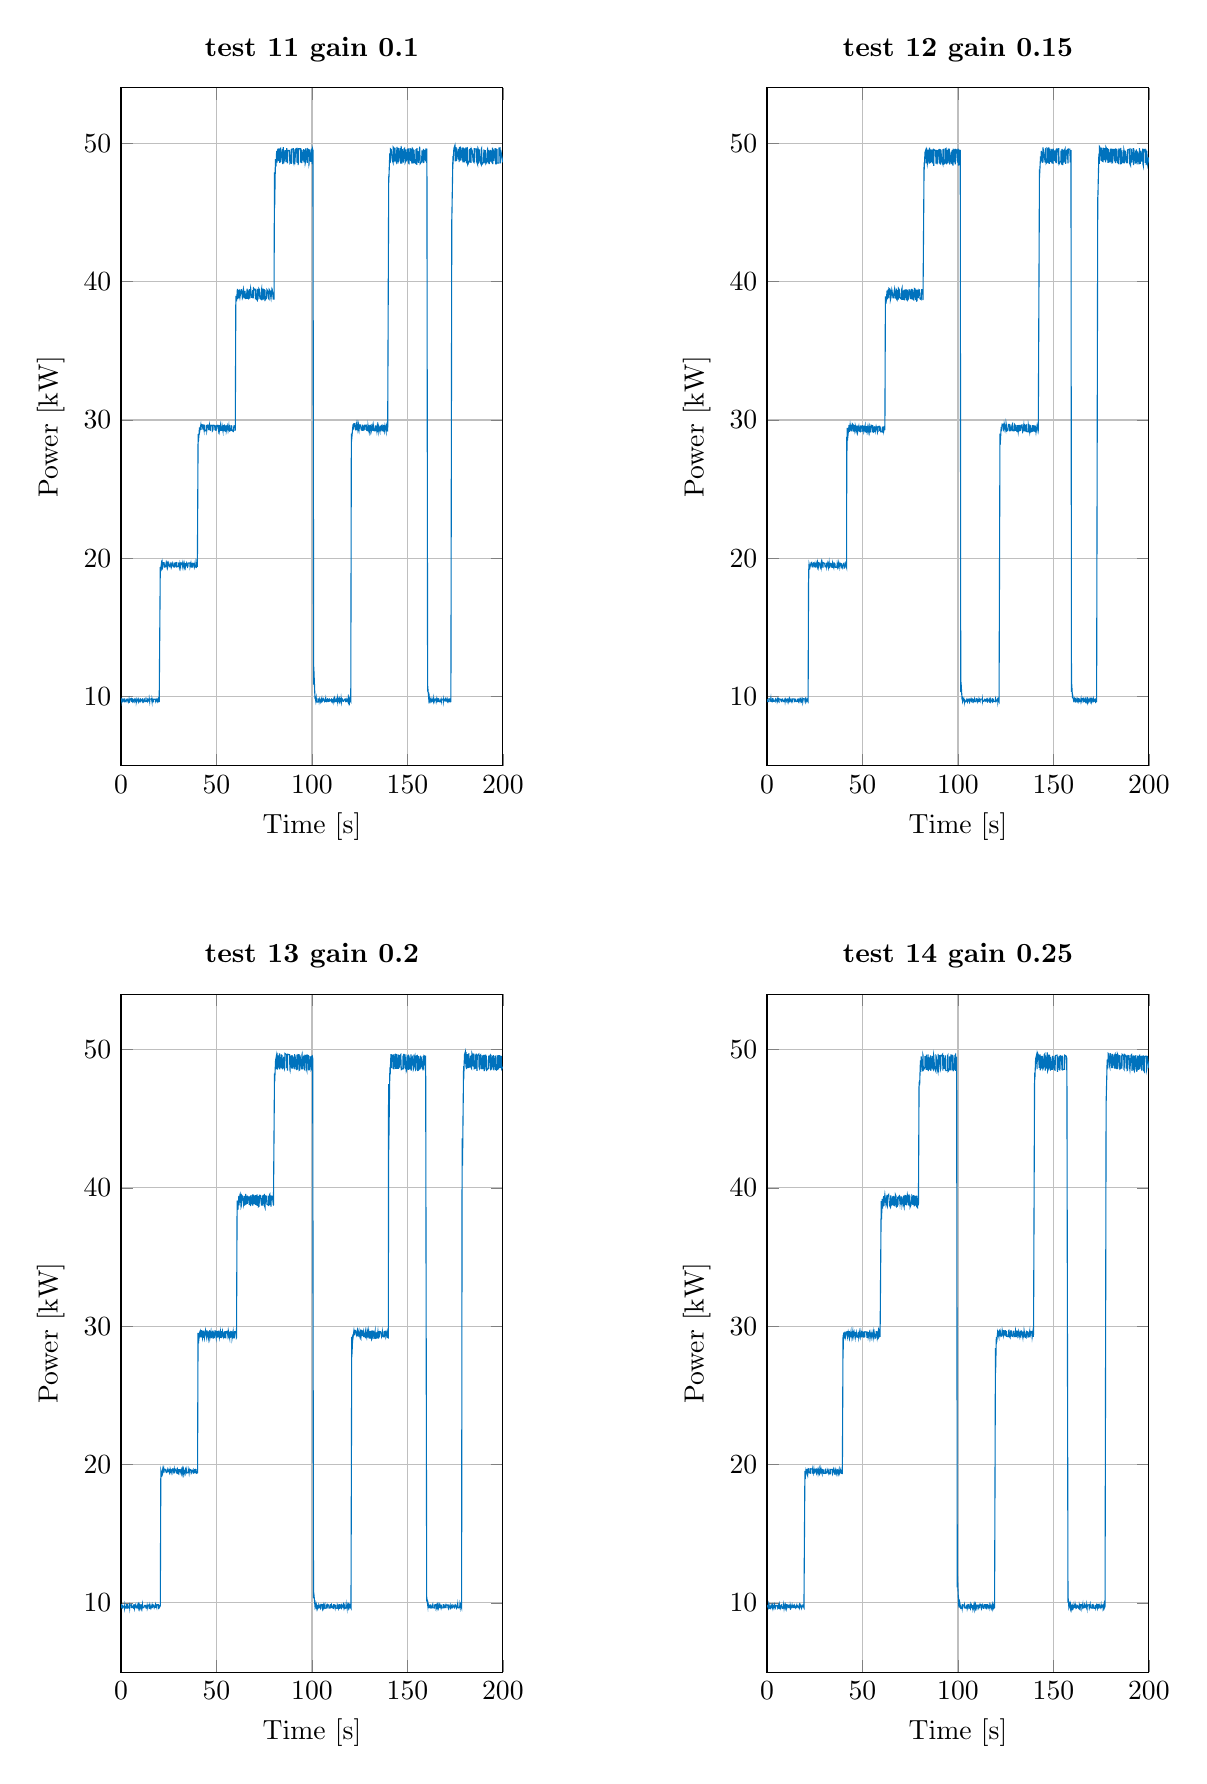
\begin{tikzpicture}

\begin{axis}[%
width=0.4\textwidth,
height=3.39in,
at={(0.953in,6.546in)},
scale only axis,
xmin=0,
xmax=200,
xlabel={Time [s]},
xmajorgrids,
ymin=5,
ymax=54,
ylabel={Power [kW]},
ymajorgrids,
axis background/.style={fill=white},
title style={font=\bfseries},
title={test 11 gain 0.1}
]
\addplot [color=mycolor1,solid,forget plot]
  table[row sep=crcr]{%
0.016	9.78898874375259\\
0.112	9.67466546965983\\
0.24	9.81788351932195\\
0.832	9.66516891927992\\
1.024	9.80578250722271\\
1.552	9.68111079887103\\
1.6	9.82204953572795\\
1.92	9.8374131646726\\
2.352	9.64019904790587\\
2.608	9.62824494679215\\
2.976	9.80983827166675\\
3.2	9.83129629346782\\
3.728	9.62472506564062\\
4.176	9.84638943047615\\
4.368	9.60766116470599\\
4.528	9.62866958328547\\
4.736	9.82104442908728\\
5.296	9.8650981041945\\
5.568	9.66153874355686\\
5.888	9.63529975670435\\
5.936	9.83921008375631\\
6.256	9.81266296286746\\
6.368	9.63453150265666\\
7.136	9.81192241893913\\
7.248	9.65537129397429\\
7.872	9.82375366185007\\
7.968	9.63192571055096\\
8.176	9.7985175554744\\
8.208	9.6404696924428\\
8.8	9.81882568688327\\
9.168	9.64844457201364\\
9.376	9.81251782499848\\
9.968	9.62449398036362\\
10.048	9.63936781341954\\
10.272	9.81408232058174\\
11.184	9.64153279103188\\
11.232	9.83943870932398\\
11.312	9.84475078948958\\
11.824	9.63306015254874\\
11.904	9.66371021585058\\
12.432	9.84049506121001\\
12.592	9.8636170358386\\
12.704	9.6421157186625\\
13.424	9.65954836006227\\
13.552	9.80643621050003\\
13.904	9.66793073146443\\
14.16	9.80800464370282\\
14.784	9.6679253791212\\
14.832	9.80226420043863\\
15.024	9.63267975175901\\
15.152	9.80524311982818\\
15.952	9.85382424546227\\
16.224	9.64086426537887\\
16.272	9.83528068972866\\
16.624	9.63983780318285\\
16.864	9.63237670773228\\
16.976	9.81899067506476\\
18.016	9.81339718015412\\
18.064	9.63046421836053\\
18.208	9.83777560307986\\
18.224	9.65615838838905\\
18.768	9.81784296354251\\
19.04	9.65527989507428\\
19.488	9.82511961339638\\
19.6	9.6310504685283\\
20	9.64576933194692\\
20.56	19.3708905493402\\
20.736	19.1462135645546\\
21.152	19.606072443916\\
21.344	19.3963513403509\\
21.6	19.6703497975857\\
21.824	19.4092760675648\\
22.16	19.6886776527951\\
22.56	19.6899273441089\\
22.784	19.3660670234119\\
23.264	19.3845197551599\\
23.632	19.6750210621164\\
24.064	19.3751748531885\\
24.272	19.7020122563309\\
24.32	19.6897534346224\\
24.464	19.3887390460668\\
24.96	19.6715240555675\\
25.504	19.3830867024849\\
25.584	19.3811502901253\\
26.16	19.6756780911262\\
26.24	19.6652446799611\\
26.384	19.3699925052935\\
27.04	19.6507319837047\\
27.424	19.3891735436609\\
27.904	19.3719537199928\\
28	19.6873555416743\\
28.224	19.3544848363087\\
28.4	19.6665729043348\\
28.912	19.688234785509\\
29.104	19.3767867320655\\
29.904	19.4172548747571\\
29.92	19.6597093627672\\
30.24	19.6329476421962\\
30.544	19.3510626026891\\
30.832	19.6451933116046\\
31.184	19.3862842593742\\
31.312	19.6634762363656\\
31.872	19.6650192546522\\
32.304	19.3810154002614\\
32.432	19.6712379640524\\
33.024	19.3581805834868\\
33.152	19.6307618128017\\
33.584	19.3775212067515\\
33.712	19.659126573667\\
33.824	19.402325734591\\
34.352	19.6495900490652\\
34.864	19.3674390295693\\
35.024	19.3945178081329\\
35.152	19.6576770222038\\
36.032	19.6589900083425\\
36.144	19.4002847047344\\
36.56	19.6470023526607\\
36.704	19.3905603748344\\
37.104	19.3659774559309\\
37.28	19.6750702064816\\
37.424	19.34937344669\\
37.632	19.6406790725322\\
38.032	19.6271993653914\\
38.384	19.3665458060244\\
38.752	19.6507816999787\\
38.864	19.385602509045\\
39.424	19.34948884508\\
39.632	19.6523895042687\\
39.984	19.3751216964435\\
40.368	28.9702524600522\\
40.512	28.4274682620181\\
41.104	29.4539751233132\\
41.248	29.2098392822724\\
41.744	29.6004240068589\\
41.888	29.2776865986266\\
42.064	29.6850835698728\\
42.544	29.6501507839323\\
42.928	29.2988347974127\\
43.024	29.6711519469278\\
43.488	29.2626282002\\
43.664	29.6606249196901\\
43.808	29.2193228233034\\
44.608	29.2187207020092\\
44.784	29.6369781966536\\
44.928	29.2525682806497\\
45.344	29.625950662763\\
45.824	29.6109524573689\\
45.968	29.2658733393234\\
46.304	29.6409009526176\\
46.688	29.2727784481391\\
46.848	29.2608285356531\\
47.024	29.6187233344019\\
47.824	29.5992526721187\\
47.888	29.2090119744306\\
48.128	29.2585143847833\\
48.224	29.6186434239785\\
49.024	29.5986973952683\\
49.248	29.2567942441381\\
49.344	29.5970953178898\\
49.728	29.2553296535973\\
49.888	29.2654337367647\\
50.144	29.5992433682848\\
50.704	29.6144472046945\\
51.088	29.2391371448774\\
51.424	29.6238215243169\\
51.568	29.2368554379912\\
52.064	29.6115916327278\\
52.208	29.2423374684843\\
52.688	29.2440915134362\\
52.944	29.5846260994525\\
53.408	29.197265064694\\
53.584	29.5786364245846\\
54.064	29.6163881080833\\
54.128	29.2396152794393\\
54.528	29.2029364230553\\
54.704	29.5662696132789\\
55.104	29.57370058137\\
55.168	29.2403396517443\\
55.664	29.5706607637646\\
56.048	29.2330940059076\\
56.464	29.5904658696066\\
56.688	29.2242463969141\\
56.784	29.6305014820219\\
56.928	29.2063894999814\\
57.488	29.246080776346\\
57.744	29.5739610422259\\
57.984	29.5599878389766\\
58.128	29.232817325329\\
58.848	29.1729518274999\\
59.104	29.5659141871331\\
59.744	29.5943435331949\\
59.84	29.2208686140937\\
60.128	38.9647989037519\\
60.512	38.5704633501257\\
60.944	39.4738718231117\\
61.072	38.7278481665633\\
61.264	39.3962803789277\\
61.712	38.793510966072\\
61.968	39.4351159189815\\
62.32	38.8887906833305\\
62.928	39.4118156886031\\
63.168	39.4187461432379\\
63.552	38.8056645505681\\
63.712	38.8665829863833\\
64.128	39.4485187027762\\
64.208	39.3873923021553\\
64.576	38.7839789269855\\
64.928	39.3211534969397\\
65.216	38.7761406284406\\
65.616	38.7843578957465\\
66.048	39.4864975552604\\
66.176	38.7490104151546\\
66.288	39.4116706037236\\
66.816	38.7088283126094\\
67.232	39.4588632494492\\
67.376	38.7776252722741\\
67.872	39.5054485614567\\
67.952	39.4264013256927\\
68.336	38.863764088747\\
68.896	38.8416001203239\\
68.992	39.3745775739886\\
69.216	38.7958730326358\\
69.392	39.5323752412649\\
70.192	39.3858912317911\\
70.4	38.7179571619821\\
70.592	39.4954590541912\\
71.04	38.7101595369083\\
71.36	38.6478276853189\\
71.616	39.4661140863577\\
71.68	38.6944807867308\\
72.176	39.4959614271415\\
72.416	39.4287728630046\\
72.72	38.7912305803814\\
73.28	38.730505252806\\
73.536	39.4096168309749\\
73.616	39.4668559810247\\
73.76	38.6387594291315\\
74.416	39.497837522224\\
74.544	38.7058603750506\\
75.056	39.4437362882567\\
75.344	38.5892188432456\\
75.44	39.4034829742204\\
75.504	38.6808887372103\\
76.144	38.7845057647966\\
76.4	39.4144175995293\\
76.8	39.3261301702534\\
77.264	38.7741245971656\\
77.504	38.7345864016568\\
77.6	39.427868057664\\
78.112	39.3207686383144\\
78.528	38.7905430337294\\
78.544	38.7790660088408\\
79.04	39.4762304997394\\
79.2	39.422526393162\\
79.728	38.742480631985\\
80.128	38.73739796439\\
80.368	47.8915034390884\\
80.448	45.3027666060487\\
80.864	48.8417186847136\\
81.152	48.3194087524265\\
81.504	49.4388707037085\\
81.712	48.59453302363\\
82.128	49.6065182361201\\
82.512	48.707259996163\\
82.688	49.6225924854518\\
83.136	48.575996060649\\
83.328	49.5848036194068\\
83.552	49.6231321567927\\
83.616	48.6402568977495\\
84.512	49.5770671584779\\
84.72	48.4894720132657\\
84.992	49.7198765936958\\
85.2	48.5401979662001\\
85.376	49.5041372011702\\
85.44	48.6863821274967\\
86.256	49.4901631201156\\
86.4	48.6311120615644\\
86.816	49.6390398107907\\
87.104	48.597658562259\\
87.264	48.6147876189793\\
87.28	49.484240678182\\
88.08	49.4825507633881\\
88.448	48.5560125135762\\
88.768	48.6161290987339\\
89.104	49.554381487247\\
89.248	48.5139101628815\\
89.424	49.5734029694482\\
90.224	49.5966566118936\\
90.352	48.6223125202158\\
90.432	48.5820612974277\\
90.624	49.5606776925079\\
90.992	48.4670269286919\\
91.488	49.5777353179128\\
92.048	49.6238120421156\\
92.192	48.5831075947955\\
92.528	49.60093154951\\
92.736	48.4226185122326\\
92.896	48.6238158098585\\
92.912	49.5979579974473\\
93.872	49.5971343445429\\
94	48.5947815798052\\
94.272	49.6090872430614\\
94.64	48.5651963661569\\
94.736	49.5030137174826\\
95.28	48.7373911044127\\
95.696	49.5690770105231\\
95.84	48.6189418664981\\
96.256	49.4930275419816\\
96.464	48.5489531580649\\
96.624	48.6497514897525\\
96.72	49.6180450859425\\
97.584	48.5780703254334\\
97.68	49.5929325378697\\
98.24	49.52206064808\\
98.448	48.4718790841808\\
98.528	48.5228197623924\\
98.624	49.5478892316835\\
99.408	48.6522939392657\\
99.664	49.6142028239683\\
100.112	48.4879952825275\\
100.224	49.6359012873998\\
100.528	49.4820886722415\\
100.88	10.8680114590886\\
100.944	12.1464303926376\\
101.536	10.0386053665772\\
101.584	10.0542753934684\\
102.032	9.65848877963446\\
102.24	9.86292344671143\\
102.352	9.62317717104482\\
103.072	9.60896722035318\\
103.184	9.846371617223\\
103.648	9.8424644017716\\
103.792	9.64783312896853\\
104.08	9.84726080306243\\
104.592	9.60705348950667\\
105.12	9.87581804681128\\
105.232	9.63207801406067\\
105.312	9.63837935242215\\
105.936	9.8494517275928\\
106.512	9.66295542216241\\
107.04	9.8608906465413\\
107.168	9.6335453866716\\
107.296	9.84022341804598\\
107.568	9.63290713803521\\
107.968	9.6495056927229\\
108.176	9.8446738366632\\
108.496	9.82713401307256\\
108.688	9.65901968802936\\
109.088	9.67631139943587\\
109.216	9.81151128763467\\
110.128	9.66021685760325\\
110.256	9.83303552339099\\
110.624	9.79839511932976\\
110.848	9.63909629873337\\
111.376	9.83494686038304\\
111.488	9.64956024723374\\
111.776	9.84599145348367\\
111.968	9.63676396961859\\
112.448	9.64874102430856\\
112.64	9.82066764846202\\
113.168	9.64536363513361\\
113.312	9.86486344928379\\
113.504	9.63969042212892\\
113.712	9.87131092072051\\
114.304	9.63088061656284\\
114.432	9.86641498706979\\
115.024	9.65196321928125\\
115.232	9.89319450218101\\
115.424	9.63609408985847\\
115.632	9.8667866404103\\
115.952	9.81710412495746\\
116.144	9.67793475335972\\
116.544	9.66739612425092\\
117.12	9.82129360457485\\
117.472	9.835024563548\\
117.664	9.64349896092876\\
118.064	9.65447364008692\\
118.256	9.80908998207301\\
118.864	9.6181559368822\\
118.992	9.85268199409662\\
119.264	9.63529306986904\\
119.392	9.85594113496999\\
119.664	9.63589910961634\\
119.808	9.83383195329344\\
120.32	9.67433569579699\\
120.624	29.0149038267143\\
120.896	28.7623592971841\\
121.504	29.6794067908426\\
121.648	29.2960048066704\\
121.824	29.715187869538\\
122.464	29.7341007336124\\
122.608	29.3583070484432\\
122.928	29.2927504371566\\
123.264	29.6399616630315\\
123.488	29.2659032715191\\
123.744	29.6348311518131\\
124.048	29.2951668320822\\
124.384	29.6556955712821\\
124.688	29.3043374661402\\
124.944	29.6440125921321\\
125.344	29.6401008959083\\
125.808	29.2794562833817\\
126.288	29.2574519098782\\
126.384	29.6210160615118\\
126.704	29.6070451874163\\
126.928	29.2615303649044\\
127.328	29.2774501487263\\
127.584	29.6233684012759\\
128.224	29.628891661384\\
128.288	29.2764898615508\\
128.464	29.6568523905772\\
128.688	29.2503894093356\\
129.248	29.2183006677882\\
129.344	29.6079126146308\\
129.808	29.2348797104583\\
129.904	29.6308501837567\\
130.368	29.2289641390226\\
130.544	29.5822215599603\\
130.944	29.6286723841154\\
131.088	29.2058766447866\\
131.824	29.6144530591621\\
131.888	29.2175770957425\\
132.144	29.6117307949485\\
132.608	29.2109409266422\\
133.088	29.2195273035822\\
133.264	29.6052230791141\\
133.488	29.1874912145717\\
133.584	29.5896085667003\\
133.968	29.2012355071738\\
134.224	29.5650436384846\\
134.688	29.1895534228589\\
134.784	29.5780271320532\\
135.568	29.1723488623098\\
135.744	29.5881940773634\\
136.048	29.1693373123708\\
136.304	29.5769119646159\\
136.624	29.6225243008884\\
136.848	29.2295502527922\\
137.328	29.2064673337591\\
137.424	29.636479642185\\
137.888	29.1987221748028\\
138.224	29.5832776781238\\
138.848	29.1584417957685\\
138.944	29.571016368047\\
139.024	29.6091440302748\\
139.088	29.216807985363\\
139.648	29.2045138229372\\
140.192	47.602745666837\\
140.208	47.1524292649028\\
140.752	49.2679297161264\\
140.96	48.5604650664398\\
141.056	49.6001894250528\\
141.536	49.5395850079759\\
142	48.8029985488856\\
142.464	48.6082360196905\\
142.576	49.7075028871676\\
142.96	49.6236408920656\\
143.024	48.6426138314977\\
143.44	49.6827186010769\\
143.744	48.7687085837904\\
144.208	48.6229485332361\\
144.48	49.7425171943797\\
145.008	48.521067580986\\
145.184	49.665105174935\\
145.328	48.6351585886786\\
146.144	49.6437650322484\\
146.432	48.5284518531525\\
146.704	49.797421054051\\
147.072	48.518607721451\\
147.248	49.5732240944644\\
147.872	48.606757921663\\
148.128	49.5789983322976\\
148.528	49.640198787389\\
148.816	48.6168080890608\\
148.976	48.6780124083839\\
149.072	49.5547419660755\\
149.696	48.6958729307818\\
150.032	49.5730202276901\\
150.432	49.580700635493\\
150.56	48.5872408109269\\
150.8	48.535345446722\\
151.376	49.6447776073833\\
151.68	48.7034500164083\\
152.016	49.6157538266959\\
152.304	48.5317007004159\\
152.576	49.6297113442992\\
152.96	49.5486259760868\\
153.024	48.5413300317266\\
153.44	49.5179848511009\\
153.744	48.6050957230121\\
154.368	48.5407329613395\\
154.48	49.5768230792499\\
154.928	48.4387387860898\\
155.024	49.6403657036197\\
155.168	48.6671010792839\\
155.424	49.4227391073289\\
155.808	48.5838000970284\\
156.384	49.7593197553446\\
156.464	49.5360605670906\\
156.672	48.5197496030111\\
157.392	48.664373357892\\
157.648	49.4749344804712\\
158.256	48.5658063531822\\
158.368	49.5965673014443\\
158.496	48.5576190778152\\
159.072	49.5086239331665\\
159.456	48.6928138302805\\
159.632	49.6198189670582\\
160.08	48.5731970535799\\
160.192	49.6033348698294\\
160.56	10.3678550796017\\
160.752	10.5199338288835\\
161.184	9.80779799177293\\
161.408	9.96923063609401\\
161.52	9.6446059061806\\
162.176	9.84382175887717\\
162.32	9.60872753114977\\
162.72	9.66042566488441\\
162.976	9.82667827122527\\
163.6	9.61991881387137\\
163.728	9.83177053287811\\
163.92	9.60737715637647\\
164.464	9.8309408452355\\
164.864	9.83968029531732\\
165.056	9.64663384544764\\
165.344	9.84939275932643\\
165.536	9.63492706064314\\
165.936	9.64944830300383\\
166.064	9.85759594067287\\
166.464	9.83338367421447\\
166.656	9.65717096056127\\
167.056	9.62252555489758\\
167.584	9.82243352558925\\
167.776	9.67241045442552\\
167.904	9.82915310977541\\
168.704	9.81688812649741\\
168.816	9.65006707251345\\
168.944	9.79900212166102\\
169.056	9.66733611486632\\
169.984	9.86709987721941\\
170.096	9.64618896050093\\
170.224	9.84463623858054\\
170.896	9.65143808458399\\
171.12	9.828090665221\\
171.632	9.65025916494746\\
171.92	9.84401059076594\\
172.16	9.8420077567264\\
172.432	9.63297076708846\\
172.752	9.63734694428484\\
173.216	44.4873169220332\\
173.232	44.3636017764039\\
173.808	49.066642073273\\
173.84	48.4894143296943\\
174.32	49.6313844131157\\
174.88	49.8489811671111\\
175.024	48.7320958465056\\
175.328	48.726675218586\\
175.44	49.7108572921066\\
175.728	48.7312992934337\\
175.824	49.6268917373825\\
176.688	48.8180261198997\\
176.864	49.598453207686\\
177.072	48.6361407764948\\
177.264	49.7108359480509\\
177.632	48.7464688906414\\
177.648	49.7576551933364\\
178.672	48.7460961949989\\
178.688	49.6777845843761\\
179.056	48.6123680342252\\
179.168	49.6983838442905\\
179.776	48.6204405679436\\
180.032	49.6188615973343\\
180.416	48.7145146317075\\
180.592	49.6972565315614\\
180.96	48.5403088022339\\
181.232	49.649502269069\\
181.392	49.6647250831027\\
181.6	48.4609807431775\\
182.4	48.7193795910501\\
182.496	49.5829591353061\\
182.784	48.6214593185881\\
183.056	49.6365693573266\\
183.264	48.5715902579537\\
183.44	49.6057399396527\\
183.92	49.4598632609769\\
184.384	48.7053678325342\\
184.768	48.6249392663008\\
184.96	49.6508366037773\\
185.088	48.6207568693257\\
185.264	49.5974767586672\\
186.144	49.5820674133226\\
186.208	48.6790292349799\\
186.752	48.4539347509353\\
186.864	49.6685702712639\\
186.944	49.647354955665\\
187.152	48.5320682440059\\
187.728	49.5608594876562\\
188.032	48.6852274258335\\
188.576	48.4807350188953\\
188.768	49.6072028286486\\
188.848	49.6356790023533\\
189.136	48.4896003735912\\
189.856	48.6206178427897\\
190.032	49.5517954716657\\
190.56	48.5406966629843\\
190.752	49.5068323300009\\
191.12	48.5429260315287\\
191.68	48.6978651835197\\
191.856	49.5565817831752\\
191.936	49.5854087569174\\
192.384	48.5363149957871\\
192.576	49.5163392878743\\
192.864	48.4929760366048\\
193.44	49.5148901303237\\
193.584	48.6698628475962\\
193.92	49.476538424609\\
194.288	48.5715364387145\\
194.56	49.6732081260976\\
194.688	48.4841388899456\\
195.024	49.5452487302904\\
195.152	48.7327184731919\\
195.904	49.6430815423484\\
196.192	48.4665589272577\\
196.384	49.6216697269203\\
196.592	48.4806827374523\\
196.928	49.5734772838201\\
196.992	48.566243892234\\
197.872	48.5624823211939\\
197.968	49.6518749913513\\
198.528	49.6648109133119\\
198.736	48.5477804802354\\
198.816	48.6464096163751\\
198.832	49.5131550692228\\
200	48.603613130148\\
};
\end{axis}

\begin{axis}[%
width=0.4\textwidth,
height=3.39in,
at={(4.183in,6.546in)},
scale only axis,
xmin=0,
xmax=200,
xlabel={Time [s]},
xmajorgrids,
ymin=5,
ymax=54,
ylabel={Power [kW]},
ymajorgrids,
axis background/.style={fill=white},
title style={font=\bfseries},
title={test 12  gain 0.15}
]
\addplot [color=mycolor1,solid,forget plot]
  table[row sep=crcr]{%
0.016	9.65747649320002\\
0.144	9.82770717674133\\
0.256	9.6461072567222\\
0.896	9.65028153904235\\
1.024	9.85351731561095\\
1.728	9.81192896237924\\
1.776	9.65087485673163\\
2	9.86170482582536\\
2.112	9.66683756912905\\
2.672	9.6320807543104\\
2.8	9.85960341779882\\
3.2	9.84688325594389\\
3.312	9.6617942319067\\
3.792	9.6560149279691\\
4.384	9.81462381625767\\
4.592	9.6659712903476\\
5.28	9.8386760945719\\
5.392	9.64374757029416\\
5.84	9.82688646911195\\
6.192	9.64216079097\\
6.272	9.62956230268871\\
6.32	9.841381744349\\
7.024	9.818351884318\\
7.488	9.65692216163625\\
7.648	9.6470749887551\\
7.776	9.82799036843103\\
8.176	9.83176380252889\\
8.528	9.64222899992495\\
8.768	9.64314202430947\\
9.344	9.81292885311926\\
9.488	9.64418119548103\\
9.696	9.81785826970592\\
10.368	9.65001504610219\\
10.496	9.83839526566526\\
11.056	9.82570029468411\\
11.168	9.63565648603875\\
11.536	9.82674824165498\\
11.648	9.62639796306747\\
11.968	9.62834329723827\\
12.08	9.83103630733357\\
12.944	9.61930331609054\\
13.072	9.86777945980773\\
13.184	9.61258973388937\\
13.312	9.84274622773319\\
14.192	9.83128037996836\\
14.304	9.64637176710688\\
14.384	9.65775840975235\\
14.432	9.82352034335454\\
14.992	9.81383276147577\\
15.184	9.6468432433479\\
15.904	9.66508998624241\\
16.032	9.8183480313264\\
16.416	9.82906395925814\\
16.544	9.65355694150228\\
17.168	9.82900546602949\\
17.344	9.64623034020624\\
17.808	9.83033195424052\\
18.08	9.64820132196708\\
18.592	9.82203444564825\\
18.72	9.61819991866852\\
19.008	9.85699161580899\\
19.888	9.83512905359286\\
19.92	9.63802194300473\\
20	9.60885353219052\\
20.208	9.8464526904122\\
20.8	9.66070400799616\\
20.976	9.817030501772\\
21.52	9.66088202381512\\
21.776	19.2347331298192\\
21.84	18.5557081066584\\
22.016	19.6011200365448\\
22.464	19.3323069428678\\
23.056	19.672519538106\\
23.376	19.7060081956421\\
23.6	19.3872345139514\\
24	19.376945461639\\
24.256	19.6585472981485\\
24.656	19.6900475889649\\
24.88	19.3760825542899\\
25.056	19.6738613565997\\
25.2	19.373548510865\\
25.6	19.366494505379\\
25.776	19.666133525687\\
26.4	19.3810273806556\\
26.528	19.6922616713729\\
26.96	19.4002397348212\\
27.088	19.6753977161431\\
27.488	19.657696908545\\
28	19.3772129999279\\
28.368	19.6566597078475\\
28.48	19.3805949179712\\
28.848	19.6974534965224\\
29.28	19.3541758961883\\
29.36	19.3594860906175\\
29.408	19.6844521418653\\
30.208	19.6341707840975\\
30.4	19.3927184897971\\
30.96	19.3747884759455\\
31.168	19.6816347632225\\
31.28	19.363636469479\\
31.808	19.6702223765086\\
32.24	19.3359804849635\\
32.528	19.6656735324338\\
32.72	19.3510258806497\\
33.04	19.3903825232667\\
33.248	19.6337701749859\\
33.888	19.5991875586029\\
33.92	19.3601429227391\\
34.32	19.3488379578824\\
34.368	19.6457428092327\\
34.96	19.3412141176385\\
35.168	19.6610356428857\\
35.536	19.615634857486\\
35.76	19.3551043775195\\
36.56	19.3561634385125\\
36.736	19.593126202962\\
36.96	19.377820606592\\
37.376	19.6305971876979\\
37.44	19.396728823378\\
38.016	19.6066104222785\\
38.16	19.3734632808734\\
38.496	19.6314216414631\\
38.896	19.6066378508419\\
39.12	19.3395160626576\\
39.36	19.2884140128543\\
39.856	19.590752974674\\
40.256	19.6389147586224\\
40.4	19.2942784469351\\
40.72	19.3309930495844\\
41.072	19.6221710381954\\
41.68	19.3286932865235\\
41.76	28.7799844290543\\
41.84	27.6135818734054\\
42.016	29.4208824864754\\
42.4	28.8966543321401\\
42.976	29.6479810174381\\
43.12	29.1421833201633\\
43.536	29.6742234749671\\
44.08	29.1780735601847\\
44.096	29.6590677798893\\
44.56	29.1727409916738\\
44.736	29.7140106838235\\
45.296	29.6118054529547\\
45.44	29.1560448081586\\
45.616	29.6174911579789\\
46.08	29.12538665342\\
46.16	29.155105777251\\
46.256	29.5695017619998\\
46.96	29.1795418584376\\
47.056	29.5605911241239\\
47.376	29.5492485924979\\
47.52	29.1589715642155\\
48.096	29.5383348785986\\
48.4	29.2019449194541\\
48.8	29.1533599982466\\
48.976	29.5594049152132\\
49.536	29.54982531218\\
49.76	29.1487254417258\\
49.936	29.6150581304273\\
50.24	29.1700250719001\\
50.496	29.5842483375049\\
50.72	29.1749920088917\\
51.376	29.5882672609425\\
51.52	29.1549303446027\\
51.92	29.1281081618642\\
52.096	29.5587701288369\\
52.4	29.1858308329815\\
52.816	29.5132390145019\\
53.04	29.1519584326859\\
53.536	29.5171920905095\\
53.76	29.1794745959419\\
54.096	29.5530187304401\\
54.32	29.1118499293733\\
54.496	29.6236619648991\\
55.136	29.5912222954264\\
55.36	29.1079628185831\\
55.536	29.5787084095614\\
55.84	29.1292746017857\\
56.24	29.1828187396741\\
56.336	29.5406282064031\\
56.72	29.1928496792694\\
57.136	29.5313573348865\\
57.76	29.1698852171342\\
57.856	29.5270129852665\\
58.08	29.1198648236896\\
58.256	29.5243965809857\\
58.896	29.5430592948945\\
59.04	29.1997682551855\\
59.216	29.5324941856188\\
59.52	29.1454614592366\\
60.24	29.1442649739497\\
60.416	29.5127757186465\\
60.8	29.0729560887565\\
60.976	29.5359987737415\\
61.12	29.1839852800118\\
61.616	29.5157075503977\\
61.728	29.2661281485842\\
62	38.9305785058535\\
62.32	38.4168454356087\\
62.896	39.3636080177707\\
62.96	38.7151404114942\\
63.536	39.4425003133235\\
63.824	38.7963854157898\\
63.856	39.5120861408629\\
64.496	39.4340416215506\\
64.624	38.6790357960774\\
64.944	38.8689954252475\\
65.36	39.4127196617508\\
65.44	39.3601978917593\\
65.984	38.8232151647252\\
66.224	38.8257025912216\\
66.64	39.34853892606\\
66.8	39.4645272272431\\
67.168	38.7777812415512\\
67.76	39.4968225381609\\
67.888	38.7175273011157\\
68.128	38.6673746303872\\
68.544	39.4028475488286\\
68.768	38.6899083569667\\
68.864	39.5082832424154\\
69.264	39.4169665861977\\
69.472	38.8525183987384\\
70.208	38.7552758273133\\
70.384	39.3643751586212\\
70.704	39.5243016799893\\
70.848	38.6780382769399\\
71.104	39.335961927316\\
71.552	38.6890042409222\\
71.744	39.4002044306757\\
71.872	38.6528072465055\\
72.384	39.4324409693532\\
72.912	38.6575273967105\\
73.088	39.4342391647485\\
73.472	38.6194456014692\\
73.648	39.3973510073978\\
73.792	38.6932101057283\\
74.272	38.8164522449742\\
74.448	39.4059223319646\\
74.928	39.3893731664959\\
75.232	38.7363189630487\\
75.808	39.4676023808825\\
76.032	38.7009835440467\\
76.128	39.4310988784543\\
76.896	38.6290714322358\\
77.168	39.5029300868737\\
77.568	39.4689667868723\\
77.856	38.6641390035486\\
78.192	39.4244923130413\\
78.336	38.5942097521262\\
78.576	38.6108407545775\\
78.752	39.4218257660927\\
79.216	38.8132609027359\\
79.552	39.4193333500586\\
79.872	39.3937729755387\\
80.096	38.7590596888384\\
80.736	38.6939952326624\\
80.992	39.4128177842657\\
81.552	39.4093034875326\\
81.616	38.6590904885932\\
81.696	38.729495507704\\
82.256	48.5963257475029\\
82.288	48.0430053151114\\
82.736	49.3357525507192\\
83.216	49.5318679414865\\
83.424	48.5399205299024\\
83.536	49.6672538119512\\
83.984	48.5258435406688\\
84.192	48.7134794501232\\
84.32	49.533523893886\\
85.008	48.5203495164646\\
85.12	49.6867841482276\\
85.648	48.5643049681478\\
85.824	49.5562972206183\\
86.448	48.6124470806968\\
86.544	49.5443649712902\\
86.832	48.5259955495144\\
87.104	49.6122219702913\\
87.312	48.3578233974264\\
87.488	49.5343865370033\\
88.288	49.4643444442604\\
88.496	48.5271481822455\\
88.768	49.5108098362135\\
89.056	48.4784951032926\\
89.136	48.5564417478976\\
89.552	49.4718654195972\\
89.952	49.5223404263742\\
90.24	48.5336699373483\\
90.592	49.5719523035987\\
90.88	48.4461730181163\\
91.056	49.5376954105982\\
91.52	48.6973776713163\\
92.064	48.4842929476451\\
92.176	49.5335595729859\\
92.48	49.5495621817775\\
92.544	48.4922696539267\\
93.184	48.5328937673568\\
93.36	49.5810458101683\\
93.76	49.6226605185011\\
94.048	48.4721170683856\\
94.128	48.5482242009354\\
94.464	49.5185369207961\\
94.848	48.5545864578216\\
94.944	49.5748335311221\\
95.424	49.5657235042507\\
95.632	48.4647236840711\\
96.448	49.3820638477661\\
96.512	48.5841477601296\\
96.816	48.5366133805674\\
97.008	49.501424858931\\
97.376	48.3798062458935\\
97.472	49.5990841341864\\
98.096	48.6214537348432\\
98.352	49.5899601234167\\
98.56	48.4721663125039\\
98.832	49.5418598353966\\
99.456	49.493744419255\\
99.68	48.5984660116184\\
100.016	49.6123692373732\\
100.304	48.3752999132339\\
100.496	49.5485170384358\\
100.784	48.4279134355814\\
101.2	49.5161105223196\\
101.456	10.3261135089008\\
101.6	11.0420620359065\\
102.192	9.7275759647973\\
102.304	10.0281549745652\\
102.432	9.63375758710863\\
103.056	9.86385274734008\\
103.408	9.61698784683193\\
103.456	9.81671327418612\\
103.648	9.63423073245645\\
104.128	9.62978926707994\\
104.656	9.81356019670282\\
105.008	9.63640722989725\\
105.28	9.80436067779656\\
105.776	9.83109859074925\\
105.888	9.61973420060808\\
106	9.83558457787876\\
106.128	9.61836571186469\\
106.816	9.8507345133006\\
107.168	9.63963962125399\\
107.408	9.6149453640034\\
107.536	9.83234616856451\\
107.856	9.80419592791253\\
108.208	9.6446008216234\\
108.64	9.82654518585846\\
108.688	9.64508093107551\\
109.408	9.63563760390067\\
109.552	9.83445211704918\\
109.872	9.85427567942723\\
110.224	9.67800718899799\\
110.352	9.83651965219477\\
110.464	9.63222255531694\\
110.944	9.65044256088211\\
111.072	9.85444564213139\\
111.584	9.67424562160125\\
111.712	9.82149429202107\\
112.592	9.82013560962932\\
112.768	9.68162682970355\\
112.832	9.83047715158881\\
113.024	9.67147721147627\\
113.584	9.65712209942943\\
114	9.82043905706562\\
114.192	9.81111437338088\\
114.464	9.69306179020912\\
115.056	9.82614567523808\\
115.184	9.65898129084253\\
115.344	9.6349270434502\\
115.456	9.82554668304731\\
116.304	9.65641452087975\\
116.432	9.81680563614855\\
116.944	9.64204566836672\\
117.152	9.83938529991834\\
117.744	9.65531443767334\\
118.064	9.61128861449027\\
118.176	9.84120198799506\\
118.448	9.82370598259292\\
118.544	9.64445173783812\\
119.44	9.66786386926243\\
119.648	9.84882836963932\\
119.92	9.64914132487026\\
120.768	9.84080055934212\\
120.88	9.61714087335262\\
121.088	9.8261719023406\\
121.52	9.66878260093132\\
122	29.0151248227416\\
122.128	28.2273568096198\\
122.64	29.5048845427346\\
122.864	29.2038056334224\\
123.12	29.7008033404625\\
123.6	29.691884518702\\
123.984	29.249089579006\\
124.064	29.2284452889137\\
124.24	29.7252893337616\\
125.024	29.2584583008077\\
125.2	29.7622722953915\\
125.28	29.6983526781889\\
125.504	29.1958923056006\\
126.144	29.2501021871162\\
126.4	29.6803950246019\\
126.96	29.670916474737\\
127.104	29.183739542195\\
127.28	29.6530820602056\\
127.504	29.2380450673854\\
127.824	29.2324860529237\\
128.32	29.6382785930486\\
128.48	29.6857936850021\\
128.704	29.2233874497507\\
129.424	29.2190065218404\\
129.52	29.7056013850258\\
129.84	29.6488001499128\\
130.144	29.2135781775121\\
130.4	29.6198518689428\\
130.704	29.2039380072175\\
131.024	29.1725631054581\\
131.28	29.6246890562972\\
131.584	29.1649753144938\\
132	29.6336505503084\\
132.224	29.1756492027889\\
132.56	29.6129789495071\\
132.784	29.2151905646176\\
133.04	29.6222278092338\\
133.52	29.6428062477012\\
133.904	29.1384998064879\\
133.984	29.1631449888628\\
134.48	29.6483735770345\\
134.784	29.1693384188779\\
134.88	29.6973562635215\\
135.504	29.1670496187807\\
135.6	29.6137918723843\\
135.92	29.6431014399512\\
135.984	29.1598329125544\\
136.784	29.1442143705594\\
136.88	29.6241960414316\\
137.504	29.1464770802359\\
137.68	29.6100571317475\\
138	29.5726271275907\\
138.224	29.140390491354\\
138.864	29.1757780240402\\
138.96	29.6182994433627\\
139.264	29.1575184878278\\
139.36	29.6232801180357\\
139.664	29.176994519368\\
139.84	29.6095706373379\\
140.304	29.1393149358341\\
140.4	29.6044461889405\\
140.864	29.0946372087695\\
141.44	29.609173211464\\
141.984	29.1753527366939\\
142.064	29.2410582267949\\
142.688	48.116834407212\\
142.72	47.6191922040313\\
143.248	49.0461851285098\\
143.472	48.6229046748563\\
143.648	49.4494126623006\\
144.416	48.5920176509648\\
144.512	49.6901963719566\\
144.576	48.6628078314646\\
144.672	49.5591137431623\\
145.68	48.6008461387644\\
145.792	49.5913000094324\\
146.096	49.6329169486848\\
146.16	48.542161457722\\
146.88	48.7114991031818\\
147.056	49.6815687288315\\
147.264	48.5563859852959\\
147.536	49.6957793385155\\
147.824	48.5068278558787\\
147.92	49.6117812574134\\
148.624	48.636005265225\\
148.8	49.5940991836878\\
149.168	48.5416632750817\\
149.36	49.5485772096599\\
149.808	48.5063321981341\\
149.904	49.6106105417388\\
150.608	48.7023529086124\\
150.784	49.4844590632187\\
151.152	48.6198668420806\\
151.408	49.582855437311\\
151.472	48.5542130522956\\
151.648	49.5893912148151\\
152.368	49.5748847018739\\
152.576	48.4935430683974\\
152.768	49.6471054177352\\
152.976	48.5009451088112\\
153.856	48.7127728548539\\
153.872	49.4686390809125\\
154.32	48.458612023505\\
154.512	49.5975979083473\\
154.88	48.4096797983758\\
154.976	49.5278180454063\\
155.6	48.5993045818916\\
155.696	49.4501351216418\\
156.096	49.594279363294\\
156.384	48.5128424834593\\
156.464	48.6426564541669\\
156.8	49.4642505535302\\
157.2	49.5109061778799\\
157.648	48.5409787636925\\
157.76	49.5799240131902\\
158.624	49.5735273170443\\
158.768	48.6201876047546\\
159.184	49.5015658329557\\
159.44	10.353765239305\\
159.568	10.8941693770639\\
160	9.89382737581241\\
160.144	10.0372399347225\\
160.576	9.71014230397133\\
161.024	9.85787357566363\\
161.216	9.63628816225739\\
161.536	9.62057072285296\\
161.664	9.82444753586244\\
162.336	9.65589302251666\\
162.448	9.85996789041156\\
162.992	9.6530659111481\\
163.2	9.85137287878218\\
163.52	9.83284528772595\\
163.792	9.63785307957671\\
164.112	9.6460927419456\\
164.4	9.83332652378083\\
164.512	9.62024804174251\\
165.04	9.86737221778618\\
165.44	9.87929497521405\\
165.552	9.62514508983575\\
165.952	9.65751996077952\\
166.08	9.82657242347281\\
166.672	9.64528716481057\\
166.8	9.83061039525767\\
167.312	9.6393781136603\\
167.52	9.79926199371086\\
167.792	9.61911584190379\\
167.92	9.8373985605793\\
168.432	9.63480712720397\\
168.736	9.83034846856875\\
169.248	9.64223402439982\\
169.456	9.87150081009034\\
169.696	9.84873596820695\\
169.968	9.64491817919118\\
170.176	9.84552587229484\\
170.688	9.67221406005187\\
170.896	9.83563344055882\\
171.088	9.66491515749816\\
171.44	9.67282820852742\\
171.616	9.81737021829198\\
172.016	9.83373180464041\\
172.128	9.60066141542351\\
172.608	9.65883528160672\\
173.2	46.0995421610033\\
173.216	45.7248648824918\\
173.792	49.2397131684759\\
174	48.510262824582\\
174.112	49.7511622097257\\
174.496	49.6552924257534\\
174.96	48.7211126183701\\
175.216	49.6810676626159\\
175.504	48.7003671930444\\
175.984	48.6718079486352\\
176.08	49.6700413003147\\
176.624	48.775359090313\\
176.72	49.6356579170895\\
177.328	48.6145496044725\\
177.504	49.7107777713561\\
177.904	49.5804616478917\\
178.128	48.7687448024191\\
178.224	49.6385412557248\\
178.592	48.5854998738555\\
178.864	49.5831475303567\\
179.152	48.5961724395766\\
179.968	49.6039084778749\\
180.032	48.6780562905927\\
180.112	48.6556372902541\\
180.448	49.6083968673056\\
180.896	48.5432812339025\\
181.152	49.545940788145\\
181.632	49.5425791264357\\
181.92	48.6836215608716\\
182.192	49.5976814150769\\
182.48	48.5569451411657\\
182.576	49.6272149675575\\
182.96	48.704280077859\\
183.216	49.5883260646612\\
183.504	48.6308314088291\\
183.984	48.5630421630367\\
184.24	49.5807503289713\\
184.72	49.566154537703\\
185.008	48.4744719044596\\
185.28	49.6569754076434\\
185.648	48.4949893269058\\
185.824	49.4898231455072\\
186.128	48.6441168351875\\
186.592	48.6116136127787\\
186.864	49.5480440721427\\
186.944	49.496513199106\\
187.072	48.5499942594088\\
187.568	49.4609054944703\\
188.032	48.6433784651055\\
188.336	48.604368826893\\
188.752	49.513214405669\\
188.816	48.5564314817281\\
188.912	49.5231896893252\\
189.712	49.5670375867461\\
189.92	48.536603769579\\
190.4	48.3857766247554\\
190.576	49.5695682777382\\
190.816	49.5398518575178\\
190.96	48.6023766919871\\
191.776	49.6376182974392\\
191.904	48.5019019179685\\
191.984	48.4133666488368\\
192.08	49.6034047537668\\
192.864	48.5307645661137\\
193.04	49.4559533765941\\
193.328	48.5860583881626\\
193.44	49.553659776065\\
193.808	48.4703846990486\\
194.064	49.3992635642131\\
194.832	48.4736164667318\\
195.024	49.6391196315156\\
195.472	48.5049407729366\\
195.728	49.4530680127007\\
196.272	48.666634603941\\
196.768	49.6071467954286\\
196.816	48.5244127078201\\
197.056	48.3787004285219\\
197.152	49.5321875799861\\
197.952	49.5589825864463\\
198.08	48.5863754124864\\
198.352	49.5498257819198\\
198.56	48.4105440394427\\
198.816	49.4604983784667\\
199.36	48.4738313081142\\
200	48.9823035644041\\
};
\end{axis}

\begin{axis}[%
width=0.4\textwidth,
height=3.39in,
at={(0.953in,2.015in)},
scale only axis,
xmin=0,
xmax=200,
xlabel={Time [s]},
xmajorgrids,
ymin=5,
ymax=54,
ylabel={Power [kW]},
ymajorgrids,
axis background/.style={fill=white},
title style={font=\bfseries},
title={test 13  gain 0.2}
]
\addplot [color=mycolor1,solid,forget plot]
  table[row sep=crcr]{%
0.016	9.79636410090723\\
0.112	9.60216323231775\\
0.24	9.8687636794016\\
0.64	9.82592649838994\\
0.832	9.65135508166753\\
1.664	9.79548893687195\\
1.792	9.62768574125493\\
1.984	9.83745527667416\\
2.192	9.63345249999931\\
2.832	9.63419229175144\\
2.944	9.8649208576115\\
3.296	9.86335238849097\\
3.408	9.62428638584032\\
3.808	9.63739913501481\\
4.336	9.86093498612331\\
4.528	9.64263555162533\\
4.656	9.86355328865005\\
5.376	9.84237668062166\\
5.488	9.62201846473504\\
5.664	9.81762228457219\\
6.128	9.67389825691098\\
6.448	9.62869114972746\\
6.656	9.8504761216219\\
6.96	9.85759672816412\\
7.088	9.60290332855729\\
7.52	9.84763398391401\\
8.048	9.63857712022099\\
8.368	9.64502044015697\\
8.512	9.84193083565282\\
9.024	9.60680411463775\\
9.2	9.86622197435759\\
9.664	9.61600598517057\\
9.792	9.84444817255487\\
10.384	9.59547909710779\\
10.512	9.86300756378714\\
10.832	9.85516992343999\\
11.024	9.64859024169858\\
11.232	9.85440680285175\\
11.344	9.63833013850448\\
11.984	9.67036226171792\\
12.352	9.8223071565448\\
12.848	9.81616483049377\\
13.024	9.6340451893047\\
13.264	9.62337409597929\\
13.616	9.8143292923701\\
13.744	9.62071321965718\\
14.112	9.82813581390181\\
14.592	9.85243818490091\\
14.784	9.6097161411691\\
15.024	9.59687987025055\\
15.152	9.86047450620418\\
15.664	9.61262200972749\\
16.208	9.85426327759536\\
16.32	9.61876753872477\\
16.512	9.87437342919529\\
16.848	9.85997124598426\\
17.36	9.63681028719504\\
17.888	9.85024726331804\\
18.08	9.64095771216877\\
18.208	9.87951741229575\\
18.72	9.66223602609709\\
18.848	9.86284112740403\\
19.568	9.87464292495307\\
19.76	9.60018117808987\\
20.08	9.64319878822968\\
20.528	9.87211247335402\\
20.576	9.86248719642055\\
20.848	19.5651725269799\\
21.28	19.2860618206232\\
21.776	19.630316964286\\
21.84	19.3908341802508\\
22.336	19.6867163823645\\
22.48	19.4138384366604\\
22.656	19.6715970607187\\
23.136	19.6564770114757\\
23.68	19.4253819521787\\
24	19.4274505061207\\
24.256	19.6883547560517\\
24.32	19.4487075999658\\
24.576	19.6721402603336\\
25.36	19.4086605830997\\
25.456	19.6759716338112\\
25.6	19.3989542460526\\
25.776	19.6521148618814\\
26.24	19.3931100564259\\
26.576	19.6288009351061\\
26.976	19.6717855392\\
27.2	19.4242380074578\\
27.856	19.7151389771382\\
28	19.4052146552796\\
28.08	19.4092637445306\\
28.256	19.6523246695119\\
28.816	19.6693514040719\\
29.12	19.3959540189858\\
29.44	19.3658441245183\\
29.616	19.631669639548\\
30.08	19.4042719263624\\
30.336	19.6333581997322\\
30.816	19.6320902110244\\
30.96	19.4041669872026\\
31.536	19.6345981890099\\
31.76	19.3738697571755\\
32.176	19.648379108675\\
32.32	19.3833755048546\\
32.656	19.6259121656944\\
32.8	19.3890918552631\\
33.056	19.6147437856663\\
33.12	19.3522308320753\\
33.696	19.6440996231775\\
33.92	19.3817697155833\\
34.336	19.6250969555828\\
34.4	19.3874415044064\\
35.12	19.412867617898\\
35.456	19.6449360632475\\
35.68	19.3965130386463\\
35.936	19.6577378093414\\
36.496	19.6164193706454\\
36.64	19.3749900872546\\
36.816	19.6215771844799\\
36.88	19.398864955529\\
37.776	19.627068258376\\
37.92	19.3768128059672\\
38.48	19.4160939324254\\
38.576	19.6301544482753\\
38.976	19.6441106750743\\
39.12	19.3739994409454\\
39.296	19.6635519778265\\
39.44	19.3636319688312\\
40.08	19.4052406324343\\
40.336	29.5182248303587\\
40.544	28.7596715588128\\
41.136	29.5261720743047\\
41.376	29.6142480330465\\
41.44	29.2300331654048\\
41.92	29.2278615391179\\
42.096	29.7054338123292\\
42.64	29.1904005466629\\
42.896	29.6723790539781\\
43.12	29.1575274611467\\
43.296	29.6685193488456\\
43.68	29.148114636569\\
44.256	29.6872106125649\\
44.8	29.2208632993081\\
45.056	29.6883602365267\\
45.44	29.1902751728761\\
45.536	29.6175846806785\\
45.76	29.1256699353868\\
46.416	29.7002089090406\\
46.56	29.1609381164561\\
47.088	29.5870386433382\\
47.28	29.1778979613544\\
47.6	29.165800825963\\
47.936	29.642525948174\\
48.256	29.6425737649447\\
48.4	29.1465525884225\\
48.8	29.1710253265135\\
49.216	29.6644437902542\\
49.296	29.6670980822181\\
49.84	29.1476292500111\\
50.176	29.6651063191924\\
50.4	29.1771145835586\\
50.656	29.6312630679314\\
50.96	29.18773568424\\
51.136	29.6673238728896\\
51.52	29.1783006325954\\
52.016	29.6136340963284\\
52.24	29.1520761167908\\
52.448	29.641132121746\\
52.64	29.1371335951254\\
53.136	29.6256352156597\\
53.6	29.210556389756\\
53.68	29.1857262731566\\
54.096	29.600656999614\\
54.24	29.1276917261928\\
54.416	29.6384512545871\\
54.88	29.1207962477195\\
54.976	29.6048493130274\\
55.616	29.6279212369617\\
56.08	29.1707454589952\\
56.16	29.1976782059998\\
56.256	29.6232485957732\\
56.88	29.1634647363356\\
56.976	29.5943786213905\\
57.36	29.1647477638249\\
57.488	29.6121573854925\\
58.016	29.5857857543245\\
58.16	29.1416700336339\\
58.688	29.6059674722977\\
58.88	29.1507454388256\\
59.36	29.1508473482759\\
59.456	29.6031478337865\\
60.176	29.6122807962724\\
60.4	29.1446947532118\\
60.48	29.1659056740366\\
60.8	39.0726112285821\\
61.2	38.3990754785945\\
61.696	39.4165155728132\\
61.76	38.7352408219798\\
62.256	39.4904447703495\\
62.416	39.550985318681\\
62.864	38.6241108554153\\
63.024	38.7012858906081\\
63.12	39.4747729160226\\
63.6	39.3883436046776\\
64.144	38.8173325716961\\
64.56	39.4118074424533\\
64.624	38.7555514923622\\
64.928	38.7810215276896\\
65.28	39.5607676620856\\
65.488	38.7840102539595\\
65.984	39.4080911351237\\
66.128	38.8407053301368\\
66.304	39.3745842511384\\
66.704	39.3252331124908\\
67.168	38.7703640726192\\
67.424	39.3856867464113\\
67.792	38.6820447410117\\
67.984	39.4633703515996\\
68.112	38.7902062160342\\
68.928	39.5245501227056\\
68.992	38.7080992080118\\
69.328	39.4969821163273\\
69.792	38.8285411221373\\
70.208	39.4408079516345\\
70.352	38.7738847196286\\
70.528	39.4670902982946\\
70.976	38.7346907361725\\
71.248	39.5205312223126\\
71.376	38.6878062169996\\
71.808	39.4022470307614\\
71.936	38.6253619231373\\
72.336	38.6664927447184\\
72.432	39.457557140086\\
72.992	39.4528439705887\\
73.536	38.7567965516852\\
73.856	38.7559480690832\\
74.032	39.4554042401668\\
74.24	38.7065156010019\\
74.752	39.4584844728713\\
74.992	39.4914255927282\\
75.12	38.6944638426779\\
75.44	38.5591118532671\\
75.616	39.4173060789711\\
76.176	39.396300864078\\
76.4	38.8111534499628\\
77.12	38.7422718729708\\
77.216	39.424339979998\\
77.664	38.729056273161\\
77.856	39.5117848987935\\
77.936	39.5361023112225\\
78.464	38.7196894559863\\
78.544	38.6387466845065\\
78.72	39.4012726901805\\
79.28	39.3836828234643\\
79.744	38.7851208865613\\
79.824	38.7732832858103\\
80.384	48.2429757422938\\
80.448	47.6317066677588\\
80.944	49.213192519518\\
81.424	49.5564562377529\\
81.552	48.5732158029818\\
81.744	49.7508572935837\\
81.872	48.5432163730703\\
82.288	49.5580772033328\\
82.816	48.6106443605656\\
83.008	49.71719911338\\
83.136	48.5606111383156\\
83.952	49.6356309851177\\
84.016	48.6398090761449\\
84.272	49.6075158464323\\
84.48	48.5553058811619\\
85.216	49.4662243642328\\
85.28	48.6905057342956\\
85.584	48.5816046403558\\
85.84	49.7121241760729\\
86.56	49.6367105013804\\
86.624	48.65520466093\\
87.04	49.6382354791895\\
87.168	48.4687436327377\\
87.248	48.6345240421927\\
87.264	49.6488703903869\\
88.304	49.620935324388\\
88.432	48.5425863410752\\
88.512	48.4951637027408\\
88.928	49.5542001055971\\
89.456	48.6199631984966\\
89.568	49.586891695907\\
89.856	48.6202777009057\\
89.952	49.5252147243947\\
90.72	48.6153105351161\\
90.912	49.6610455341207\\
91.04	48.5507422746587\\
91.136	49.5592482939366\\
91.984	48.5010497503314\\
92.176	49.6267332128714\\
92.384	48.5405981433807\\
92.8	49.6262522106154\\
93.2	49.6207176530994\\
93.328	48.4948805918957\\
93.648	48.533814608292\\
93.744	49.5702113404581\\
94.592	48.5663364464725\\
94.704	49.5705043946903\\
94.784	49.619414068154\\
94.992	48.5673333603492\\
95.648	49.5568742874643\\
95.936	48.5756151769064\\
96.256	48.5275343160128\\
96.352	49.5737250634171\\
96.832	49.5582353912595\\
97.2	48.5351395013689\\
97.36	48.4515139128443\\
97.456	49.5974692710759\\
98.096	49.5512400310306\\
98.304	48.4817065660712\\
98.496	49.535584639609\\
98.624	48.498426660714\\
99.44	49.5166948440104\\
99.568	48.5205213484269\\
99.888	48.6037760070556\\
100.064	49.5970330175662\\
100.384	49.3464882615619\\
100.8	10.3533853387255\\
100.944	10.7319834301669\\
101.552	9.80787592830803\\
101.728	9.96784923621042\\
102.16	9.65039786595166\\
102.336	9.86735693147675\\
102.8	9.61197376525891\\
102.992	9.84919732930236\\
103.12	9.63317562120312\\
103.52	9.63204854469952\\
103.632	9.86638585522334\\
104.4	9.6256979069402\\
104.592	9.88290507946508\\
104.72	9.58869152823249\\
104.848	9.89281900742746\\
105.488	9.87872374811573\\
105.6	9.60408376069723\\
106.112	9.86135770181031\\
106.256	9.63213093839452\\
106.784	9.85343168463516\\
106.896	9.61551773435223\\
107.616	9.61812373318028\\
107.744	9.88403612226634\\
107.936	9.60248356106065\\
108.064	9.89631829084185\\
108.752	9.83619435913337\\
108.896	9.63173901462365\\
109.536	9.62223994939981\\
109.664	9.86198943055236\\
110.064	9.86162817712715\\
110.176	9.61901564719274\\
110.304	9.83608968213927\\
110.816	9.64106230934436\\
111.216	9.61250749401712\\
111.328	9.86322718769102\\
111.648	9.86302945344646\\
112.096	9.61855040532044\\
112.288	9.86192017360992\\
112.416	9.62281231010293\\
113.136	9.61061855086079\\
113.264	9.84952338307873\\
113.856	9.6172664329028\\
113.968	9.85388715763031\\
114.32	9.86572174002439\\
114.432	9.61139769054889\\
114.832	9.63034082028445\\
115.04	9.84741854263577\\
115.36	9.88024101602457\\
115.552	9.64410182228586\\
116.4	9.90043009586514\\
116.512	9.60867655297771\\
116.64	9.89338740706275\\
116.832	9.62431723226816\\
117.28	9.86268040726623\\
117.472	9.61204882511953\\
118.112	9.65706596910417\\
118.24	9.8526185442377\\
118.432	9.62756479320102\\
118.576	9.85520452818075\\
119.072	9.63992866073489\\
119.2	9.86457573672198\\
119.712	9.67606167247279\\
119.84	9.83933829375517\\
120.432	9.64075941161121\\
120.832	29.2198975793186\\
120.944	27.9811712182897\\
121.408	29.4010900215883\\
121.52	29.1928664555104\\
121.968	29.6673622984477\\
122.272	29.3397266540001\\
122.368	29.6969896196816\\
122.768	29.689836012151\\
123.312	29.3721807007179\\
123.728	29.6597744439486\\
123.872	29.3124791943468\\
124.112	29.2893656716042\\
124.288	29.6282699493099\\
125.072	29.2415621218152\\
125.168	29.5822672693247\\
125.664	29.2413400520788\\
125.808	29.697515586492\\
126.288	29.648093592137\\
126.432	29.2937536537047\\
126.688	29.6949373400623\\
126.992	29.2149926265616\\
127.168	29.5691667940494\\
127.536	29.2574246552543\\
127.952	29.1986778972623\\
128.08	29.6039663043693\\
128.656	29.2179254879774\\
128.928	29.72770833392\\
129.008	29.6869269622657\\
129.136	29.1720703855596\\
129.648	29.6573449404526\\
129.936	29.1021184264326\\
130.368	29.6459185089397\\
130.576	29.1051325168663\\
131.008	29.6746144386748\\
131.216	29.0400439487762\\
131.536	29.1299557097209\\
131.648	29.6489730182137\\
132.288	29.630664848422\\
132.416	29.0889446879811\\
133.088	29.6395003374642\\
133.216	29.1124908392797\\
133.856	29.1455166807375\\
133.968	29.593683357421\\
134.096	29.1206518879598\\
134.528	29.6055949235052\\
134.816	29.1063438531943\\
134.928	29.6294707457039\\
135.216	29.1936804443351\\
135.392	29.6156503614426\\
135.872	29.5995752574335\\
136.416	29.2521641109088\\
136.832	29.6033837901157\\
136.976	29.2507235159995\\
137.152	29.6400943075076\\
137.296	29.2296382540984\\
137.936	29.233579765665\\
138.112	29.620911077697\\
138.512	29.6323792354577\\
138.704	29.2411821677929\\
139.312	29.5870713614561\\
139.536	29.1878812099106\\
140.016	29.1537140392956\\
140.112	47.4850763789135\\
140.208	42.757979450411\\
140.8	48.7075411048034\\
140.944	48.1847504329604\\
141.36	49.6556185163873\\
141.488	48.6419696472288\\
141.664	49.6002025988765\\
142.224	49.5761980972933\\
142.432	48.6458246912485\\
142.752	48.6159530598554\\
142.848	49.6473536575591\\
143.616	48.5994515122619\\
143.728	49.6996264227961\\
144.016	48.5905527346863\\
144.112	49.6621557600138\\
144.656	48.5904115073433\\
145.072	49.6462546781641\\
145.36	48.5876481744848\\
145.696	49.5846794387778\\
145.92	48.6830786255912\\
146.016	49.5510060411859\\
146.496	49.6323697749298\\
146.784	48.540662011692\\
147.568	48.6255304322091\\
147.68	49.5426709065265\\
147.888	48.5522328177565\\
148.064	49.6396597168002\\
148.304	49.6361597345997\\
148.912	48.5809419878843\\
149.184	49.634118346635\\
149.392	48.4422143639161\\
149.952	48.6746585893259\\
150.128	49.5325599258378\\
150.448	49.5625973235935\\
150.576	48.5149467637622\\
150.832	49.5471993400266\\
151.376	48.5636210747535\\
151.872	49.6357639226715\\
152	48.4679930920986\\
152.08	48.5337689655921\\
152.576	49.4459825958524\\
152.976	49.5233893311445\\
153.104	48.5528165528737\\
153.344	48.6385339235777\\
153.84	49.5454268803138\\
153.92	49.5758392736949\\
154.288	48.5196691615824\\
154.528	48.5635093184567\\
154.624	49.5227620893414\\
155.184	49.5606683562503\\
155.392	48.4836724664682\\
155.792	48.5038273830931\\
155.888	49.5121506165548\\
156.512	48.5510085514571\\
156.928	49.5551396239404\\
157.056	48.610668155925\\
157.152	49.4769431568566\\
158.16	48.4863604100059\\
158.272	49.5106337999281\\
158.48	48.5495763998946\\
158.576	49.5626359623187\\
159.216	49.503666291281\\
159.424	48.4449829822899\\
159.536	49.550538479622\\
160.08	10.1145037118054\\
160.208	10.2848771741641\\
160.704	9.74616750037856\\
160.832	9.96491554560672\\
161.344	9.66914365109085\\
161.744	9.65281030501467\\
161.84	9.84905703532175\\
162.192	9.84712928511011\\
162.384	9.63105583075494\\
162.704	9.64259368003054\\
163.248	9.8798995892468\\
163.36	9.64832398002759\\
164.08	9.6311509726132\\
164.192	9.84977675928751\\
164.848	9.87542704398206\\
164.96	9.62512581247571\\
165.488	9.86667203764863\\
165.6	9.61061073701125\\
166.048	9.84675191985187\\
166.24	9.61742074738896\\
166.768	9.84962014666456\\
166.96	9.63499446637096\\
167.072	9.8410297480571\\
167.52	9.64224342848208\\
167.664	9.87114230066327\\
167.84	9.62087764983454\\
168.576	9.65256278706825\\
168.704	9.86398898670676\\
169.104	9.87344164708675\\
169.216	9.6466251545699\\
169.536	9.66107059435578\\
170.064	9.84571798588311\\
170.176	9.63345017555725\\
170.304	9.84597719579631\\
171.104	9.8575422562132\\
171.216	9.61528776348077\\
171.408	9.87122005397911\\
171.536	9.60519795161549\\
172.368	9.85969600726194\\
172.512	9.59653045010326\\
172.832	9.64968972301746\\
173.2	9.84176504037219\\
173.36	9.85766783174962\\
173.472	9.65556782143326\\
174.32	9.8218306252739\\
174.432	9.66547929734697\\
174.512	9.64792058742025\\
175.04	9.80389339275462\\
175.12	9.82943224014789\\
175.632	9.62791315815487\\
176.096	9.85880181768613\\
176.272	9.64560534978826\\
176.4	9.85924484006416\\
176.592	9.63752972917611\\
177.328	9.6562853195941\\
177.456	9.86016520641638\\
177.648	9.66087009574079\\
177.856	9.87616151151641\\
178.368	9.63896861700844\\
178.624	43.5736066586891\\
178.832	41.6062506433582\\
179.408	48.7904586582794\\
179.456	47.8884279931914\\
179.872	49.6215849621378\\
180.336	49.839121227787\\
180.624	48.7044253400442\\
180.736	49.8180432958231\\
180.944	48.5824126747904\\
181.36	49.6600824148983\\
181.744	48.6499135651178\\
182.16	49.7311352778455\\
182.288	48.6658688458573\\
183.104	49.5531986144071\\
183.152	48.743857354386\\
183.552	48.6346491043043\\
183.728	49.7413227083742\\
184.048	49.6141310486448\\
184.224	48.7844093613459\\
184.768	49.7033284439134\\
184.896	48.5963475342936\\
185.536	48.634284267594\\
185.632	49.629482615617\\
185.84	48.6164271367397\\
186.032	49.687788844117\\
186.4	48.4471420014893\\
186.576	49.5625419198707\\
187.376	49.6669334080872\\
187.504	48.6946202317898\\
187.664	48.6431645325037\\
187.76	49.5147473221188\\
188.32	49.6057217512946\\
188.448	48.6154109214004\\
188.928	48.6049172989667\\
189.104	49.5876793354007\\
189.712	48.580248982808\\
189.904	49.5978889573203\\
190.192	48.4284798248064\\
190.288	49.5625713795987\\
190.928	49.5873502402801\\
191.056	48.5320164519175\\
191.328	49.5443046661333\\
191.536	48.5037774191917\\
192.4	48.6293007344876\\
192.512	49.5549293855104\\
192.64	48.5970364698293\\
192.816	49.4887294828383\\
193.456	49.5966441876743\\
193.584	48.4884007117502\\
193.776	49.5962836478804\\
193.984	48.5380314160553\\
194.64	49.526384234014\\
195.008	48.543828521203\\
195.04	49.5904491940657\\
195.248	48.4900590161908\\
195.984	49.5183150221039\\
196.192	48.523445662397\\
196.304	49.5770970462265\\
196.592	48.5065833539123\\
197.152	48.5549161740213\\
197.328	49.594041080329\\
197.776	48.5669397790053\\
197.952	49.549235608603\\
198.432	49.5388402861435\\
198.576	48.6697558945185\\
199.152	49.5373600986585\\
199.28	48.5674802010967\\
200	48.7310756684696\\
};
\end{axis}

\begin{axis}[%
width=0.4\textwidth,
height=3.39in,
at={(4.183in,2.015in)},
scale only axis,
xmin=0,
xmax=200,
xlabel={Time [s]},
xmajorgrids,
ymin=5,
ymax=54,
ylabel={Power [kW]},
ymajorgrids,
axis background/.style={fill=white},
title style={font=\bfseries},
title={test 14  gain 0.25}
]
\addplot [color=mycolor1,solid,forget plot]
  table[row sep=crcr]{%
0.016	9.83014236521101\\
0.608	9.65491523864908\\
0.736	9.82502882636745\\
0.928	9.59837464163166\\
1.344	9.60292475506301\\
1.472	9.83416442533841\\
1.984	9.62287630341425\\
2.48	9.83288212324703\\
2.944	9.60834066668097\\
3.056	9.83382405160993\\
3.584	9.63981135313415\\
3.728	9.85496248972184\\
3.84	9.6407841582782\\
3.968	9.84777045196761\\
4.4	9.64349668629224\\
4.768	9.82071305250601\\
5.408	9.81939407395097\\
5.6	9.65144152604459\\
6.048	9.82953275470803\\
6.16	9.60589625077925\\
6.4	9.59272333135603\\
6.528	9.87726593199798\\
6.976	9.60954205703621\\
7.504	9.84937075360533\\
7.744	9.86343696542507\\
7.936	9.59583265573104\\
8.576	9.62204898637583\\
8.704	9.82217861205924\\
8.896	9.61970796840191\\
9.088	9.82311335543949\\
9.536	9.61825293407827\\
9.76	9.84752969470747\\
10.192	9.6082746997582\\
10.32	9.86980937311098\\
10.64	9.85489076635807\\
11.072	9.66049880693632\\
11.312	9.67247652560545\\
11.488	9.80318113859312\\
12.032	9.6358053656797\\
12.16	9.84845620061163\\
12.512	9.63574235488624\\
13.04	9.84734979965562\\
13.168	9.62578941026068\\
13.28	9.84094093343682\\
13.776	9.83602546748609\\
13.888	9.66640828141997\\
14.368	9.65966562271184\\
14.496	9.80812971959723\\
15.008	9.63657793935906\\
15.536	9.83408839332066\\
15.648	9.632696534266\\
15.76	9.82487774790767\\
16.784	9.62648398949433\\
16.832	9.83667571643322\\
16.912	9.86321576722125\\
17.024	9.63231533615603\\
17.632	9.85015192195559\\
17.984	9.66509092562059\\
18.112	9.82491772864399\\
18.224	9.65171985653523\\
18.752	9.82563809987973\\
19.344	9.6530427454349\\
19.84	19.5404576274496\\
19.984	18.9464595713765\\
20.4	19.6005569379725\\
20.944	19.3500782238377\\
21.056	19.6680388205752\\
21.344	19.3575825421177\\
21.536	19.7043232087809\\
21.856	19.6841720852652\\
22	19.4155433023899\\
22.64	19.3768738550574\\
22.736	19.6923421967825\\
23.568	19.6804381819285\\
23.68	19.350015775644\\
23.808	19.658593609503\\
24.24	19.3766184945997\\
24.528	19.6514174576494\\
24.72	19.3819365820682\\
25.12	19.4010095030373\\
25.168	19.6557113873829\\
25.808	19.6736706067344\\
26	19.3857368237241\\
26.608	19.6591741957389\\
26.8	19.3352487082354\\
27.328	19.6635107236395\\
27.44	19.3626207203956\\
27.52	19.3228918162723\\
28.048	19.6636194985916\\
28.16	19.3381642582156\\
28.288	19.6846357999754\\
28.88	19.3394704771064\\
29.056	19.6329178159439\\
29.536	19.6033462881988\\
29.68	19.3682879278777\\
30.4	19.3605959434627\\
30.496	19.6209192808465\\
30.576	19.6326514806687\\
30.64	19.3625397825233\\
31.36	19.3976324264024\\
31.536	19.6270114350214\\
32.24	19.3677474876499\\
32.416	19.7067262437137\\
32.56	19.3357699009068\\
33.2	19.3307334574201\\
33.376	19.6529908609499\\
34.192	19.6510316682022\\
34.24	19.3613678539326\\
34.32	19.3169638576591\\
34.912	19.6736102157248\\
35.52	19.3024836448145\\
35.6	19.2937435153814\\
35.792	19.6295398431866\\
36.48	19.3169700384618\\
36.592	19.6390483321391\\
37.024	19.6134122704006\\
37.28	19.3603848357791\\
37.744	19.6346312730622\\
37.856	19.3396184953935\\
38.544	19.6269626753453\\
38.656	19.3671704312373\\
38.864	19.6306642124075\\
38.976	19.3610906605766\\
39.456	19.3515312733834\\
39.824	29.3754453695233\\
39.92	28.3181957582216\\
40.112	29.5374145599931\\
40.576	29.1114698309695\\
40.752	29.5966478075687\\
41.136	29.2268098707677\\
41.552	29.5805845754548\\
41.952	29.5955250587994\\
42.176	29.2542083867089\\
42.512	29.5715671858939\\
42.976	29.2259181586531\\
43.072	29.6448267240123\\
43.296	29.178412381747\\
43.952	29.6249662298122\\
44.096	29.2028389022579\\
44.272	29.5955810949925\\
44.496	29.2029416520345\\
44.912	29.6228756990621\\
45.136	29.2300314009176\\
45.632	29.5750072853005\\
46.096	29.205541861472\\
46.272	29.5610862384695\\
46.336	29.2420787166078\\
46.752	29.5607757112102\\
47.136	29.1979872113835\\
47.616	29.2233550284597\\
47.792	29.5834083186442\\
48.016	29.2040716960765\\
48.352	29.5846120971601\\
48.816	29.220288310369\\
49.152	29.5926658162991\\
49.536	29.1925989644818\\
49.632	29.6047508537849\\
50.032	29.5850720758678\\
50.256	29.2443848932007\\
50.576	29.2195952551992\\
50.752	29.5995928187702\\
51.136	29.1981889596222\\
51.312	29.594555901526\\
52.112	29.5791251342198\\
52.336	29.1907302030548\\
52.736	29.1724525819811\\
52.832	29.5479511954194\\
52.992	29.5375363135384\\
53.056	29.2229914383006\\
53.632	29.5410393043582\\
53.936	29.1195190663394\\
54.432	29.539553286666\\
54.816	29.2220015839659\\
55.072	29.538076442178\\
55.136	29.1975577067063\\
55.552	29.5697949320181\\
55.696	29.187317527188\\
56.112	29.5488399946049\\
56.576	29.1235956978574\\
56.976	29.1797505751641\\
57.152	29.6042327473904\\
57.632	29.5894474794874\\
57.776	29.209757612525\\
58.192	29.5667089203221\\
58.336	29.1528973953789\\
58.656	29.2226116234753\\
58.752	29.5852445288046\\
59.216	29.2318204038007\\
59.792	39.033162055273\\
59.92	37.712295352502\\
60.352	39.2043975655397\\
60.496	38.4988022432692\\
61.072	39.3929657069728\\
61.216	38.6758971868148\\
61.632	39.3949796287094\\
61.712	39.4962752970657\\
62.256	38.8434249248243\\
62.832	39.4905337672288\\
62.896	38.7734348387118\\
62.976	38.7302940125247\\
63.072	39.3558404157867\\
63.712	39.5101644277919\\
64.16	38.714674594242\\
64.64	38.5894677859406\\
64.816	39.4533041531508\\
64.96	38.6733283562772\\
65.776	39.3825229904985\\
65.84	38.7386604774763\\
66.336	39.4187058614676\\
66.4	38.7366329472076\\
67.024	38.6974102939477\\
67.216	39.5158220930212\\
67.536	39.4101203753032\\
67.904	38.6273553734061\\
68.224	38.6655068613621\\
68.48	39.3345858371069\\
68.624	38.7324563777156\\
68.72	39.3227529146156\\
69.28	39.4133904614544\\
69.664	38.8404610993751\\
70.16	39.4026382624138\\
70.384	38.7772378867221\\
70.48	39.3310750031721\\
70.704	38.7626731445454\\
71.52	39.4224666905088\\
71.568	38.7431203134118\\
71.808	38.5981327177262\\
72.224	39.4860093606407\\
72.288	38.7720522862543\\
72.864	39.4566585825231\\
73.008	38.7379421420197\\
73.504	39.4898249861164\\
73.584	39.4345023834226\\
74.112	38.7327291702082\\
74.384	39.5205278516661\\
74.512	38.7139893612735\\
74.784	39.4347640673706\\
74.912	38.5974313874761\\
75.472	38.780862270605\\
75.888	39.4379226824714\\
76.128	39.3750360954623\\
76.352	38.7670529350139\\
76.848	39.4691964428231\\
77.056	38.65586483512\\
77.648	39.4150558647632\\
77.856	38.709016596427\\
78.288	39.4266168516845\\
78.416	38.6327938876754\\
78.816	38.5724307223364\\
79.152	39.3933813006598\\
79.296	38.724140074375\\
79.632	47.6781202448495\\
79.92	47.4067361547468\\
80.352	49.2089393828264\\
80.56	48.3836751957141\\
80.736	49.4924776925254\\
81.504	48.4591533135979\\
81.616	49.6305578635283\\
81.696	49.5869605659435\\
81.824	48.5028239729699\\
82.624	48.6724823612611\\
82.72	49.5129001506483\\
83.408	48.5238539442294\\
83.504	49.6226585963377\\
84.112	48.5017788952446\\
84.384	49.6441081246769\\
84.512	48.425323454377\\
84.768	49.4492787176007\\
85.232	48.5372837585272\\
85.648	49.573801368921\\
85.776	48.4459728693738\\
86.512	49.5079377455197\\
86.576	48.6717294926083\\
87.12	48.5426633186704\\
87.216	49.6273739995181\\
87.296	49.5698806493538\\
87.76	48.6287637361916\\
88.384	48.423603751147\\
88.48	49.5602859189653\\
88.56	49.5484894500262\\
89.104	48.614780622524\\
89.488	48.3956950076673\\
89.6	49.6827257008391\\
89.808	48.3439703074086\\
90.304	49.5499075248219\\
90.704	49.5568490154324\\
90.912	48.5856005713243\\
90.992	48.6243917459959\\
91.008	49.4762705802877\\
91.968	49.6596756689632\\
92.096	48.468152541709\\
92.272	49.5870616673493\\
92.816	48.5928364593068\\
93.312	49.5692251317442\\
93.44	48.4882861371703\\
93.536	49.5762176805642\\
93.68	48.4663952570841\\
94.544	48.4669951598839\\
94.656	49.5785409016105\\
94.736	49.5983612623033\\
94.864	48.4183239353097\\
95.584	48.5593127805773\\
95.68	49.4993470029289\\
96.208	48.4833664992156\\
96.304	49.5972260286913\\
96.944	49.5858947348677\\
97.152	48.4909158134932\\
97.344	49.5898196767167\\
97.632	48.4885845132381\\
98.192	48.576502905086\\
98.368	49.5433819611854\\
98.688	49.6210557386341\\
98.816	48.4537456827819\\
99.312	49.4685618856672\\
99.632	11.1263099483638\\
99.712	11.9600835915856\\
100.288	9.98650567561587\\
100.48	10.1415422089417\\
100.912	9.65456748629588\\
101.056	9.92144925778794\\
101.472	9.59115568564567\\
102.048	9.60307294145147\\
102.176	9.88358648987735\\
102.288	9.65535807008925\\
102.496	9.86605189598993\\
103.184	9.82701979008097\\
103.328	9.61222797660888\\
103.456	9.85452778731031\\
103.888	9.63038348024625\\
104.528	9.62991914581396\\
104.656	9.86739375774712\\
104.848	9.60117448527148\\
105.28	9.88177883451136\\
105.552	9.8717290053339\\
105.744	9.60478747509365\\
106.064	9.62741460762215\\
106.432	9.8647321236969\\
106.624	9.61530258622089\\
107.072	9.84761883448193\\
107.584	9.61868968503875\\
107.776	9.83843283632479\\
107.904	9.57771363048631\\
108.336	9.86266388165328\\
108.544	9.62109005575163\\
108.688	9.86193757927613\\
109.12	9.62075316230833\\
109.248	9.8800536855276\\
109.76	9.64036977145884\\
109.888	9.83951643821129\\
110.528	9.84398592037523\\
110.64	9.60851243374626\\
111.424	9.86823099955324\\
111.536	9.60216555599789\\
111.712	9.87297981086214\\
112.304	9.86130485930204\\
112.416	9.61663065598868\\
112.944	9.85339455531885\\
113.376	9.60926304986611\\
113.696	9.62183435158159\\
113.824	9.8692952095877\\
114.48	9.86348912951446\\
114.592	9.60097598260185\\
114.912	9.57892597319953\\
115.04	9.87772917462643\\
115.36	9.87930074866561\\
115.792	9.63772315273952\\
116.32	9.847188703651\\
116.432	9.60794736638812\\
116.56	9.85310872263544\\
116.752	9.62404825699303\\
117.184	9.85397639661251\\
117.632	9.60037155046385\\
118.08	9.86775469641034\\
118.272	9.57552230103296\\
118.736	9.85292890947241\\
118.928	9.62434250882377\\
119.168	9.65731774740267\\
119.632	28.4031980988289\\
119.696	26.6247365442914\\
120.096	29.2102453246423\\
120.288	28.8378612123036\\
120.784	29.5927683441208\\
121.408	29.2369409944527\\
121.504	29.644313515036\\
121.904	29.7189766669196\\
122.048	29.2702086767511\\
122.144	29.6852382759782\\
122.608	29.2657074726891\\
123.008	29.3090744573423\\
123.184	29.6974902773005\\
123.728	29.337321476914\\
123.904	29.7085686849985\\
124.128	29.2863611145532\\
124.464	29.6626490328256\\
124.784	29.6674966749257\\
125.088	29.2663614425544\\
125.264	29.6552215297178\\
125.488	29.2635083186168\\
126.288	29.2412918824602\\
126.464	29.6410078015701\\
126.624	29.6781654246926\\
126.928	29.2569191083489\\
127.328	29.1636423459236\\
127.504	29.6533666594954\\
127.904	29.657372832906\\
128.048	29.3042714243128\\
128.768	29.2532967545417\\
128.864	29.6159369850065\\
129.184	29.6276453774792\\
129.568	29.2449661194066\\
129.888	29.2463671039339\\
130.144	29.6609230336918\\
130.608	29.2170823120103\\
130.704	29.632732327609\\
131.264	29.6319741963169\\
131.408	29.2036154240921\\
131.488	29.2139576980192\\
131.824	29.6004008823339\\
132.368	29.2372882986866\\
132.704	29.6453228531107\\
132.928	29.168066527278\\
133.104	29.6534807869941\\
133.504	29.6046430571763\\
133.968	29.2055609481034\\
134.144	29.5908475109988\\
134.368	29.1700366587003\\
134.624	29.6863008796545\\
135.168	29.2226614281826\\
135.648	29.1650033721626\\
135.824	29.6757918789986\\
135.888	29.2106678323583\\
136.224	29.5973578095537\\
136.624	29.5881688722222\\
136.768	29.213685505607\\
137.088	29.2357680819327\\
137.584	29.6476337442092\\
137.728	29.2005188253857\\
138.064	29.5991557145335\\
138.624	29.61410455106\\
138.848	29.2088394160902\\
139.264	29.6263097637408\\
139.488	29.2218370903491\\
139.584	29.6118025816921\\
140.128	48.3240374169053\\
140.256	47.8143655365584\\
140.672	49.3175593055188\\
141.232	49.6401426252783\\
141.44	48.5725810639324\\
141.552	49.7739824289417\\
142.176	49.577694667295\\
142.56	48.6771032723942\\
142.976	49.6340384690233\\
143.104	48.4952380164226\\
143.44	49.5380591138577\\
143.824	48.6099993328688\\
144.16	49.5296920745869\\
144.528	48.6018186965795\\
144.928	48.7484246965623\\
145.104	49.5983439411603\\
145.504	49.6853926650278\\
145.712	48.4600913708703\\
145.808	49.5725357669779\\
146.352	48.6154532323551\\
146.768	49.7786193763831\\
146.976	48.4526100431701\\
147.376	48.6243000135482\\
147.552	49.5772616787169\\
147.952	49.5753302700456\\
148.24	48.5416935242689\\
148.32	48.5319990792226\\
148.336	49.4539848314445\\
148.96	48.5159040067591\\
149.456	49.5371393987466\\
149.584	48.5157747450435\\
149.76	49.5102578034166\\
150.528	48.4997223044213\\
150.784	49.5044550681204\\
150.848	48.4433046059525\\
151.024	49.555528395712\\
151.904	49.5875811773275\\
152.032	48.4430639499478\\
152.112	48.3809548224296\\
152.288	49.499779753211\\
153.056	48.5210687191008\\
153.168	49.5303249699362\\
153.376	48.4761761550254\\
153.632	49.5373703408503\\
154.192	49.4781074856092\\
154.48	48.5295218593599\\
154.592	49.5464793105753\\
154.72	48.5205866395039\\
155.584	48.5745535987845\\
155.696	49.524977028004\\
155.824	48.5305600506634\\
155.92	49.5802744376862\\
156.8	49.5040034980747\\
156.928	48.4954880003603\\
157.04	49.3888684738091\\
157.616	10.0448038446795\\
157.712	10.3338601139011\\
158.08	9.68391522622552\\
158.496	9.93512270963863\\
158.88	9.6280097211309\\
159.008	9.89269755668989\\
159.44	9.60188589303687\\
159.568	9.87401598858573\\
159.76	9.60845682123766\\
160.208	9.84691615302028\\
160.336	9.60622836104193\\
161.104	9.86300229896439\\
161.296	9.63123610243965\\
161.424	9.88177144957739\\
161.856	9.60447312484325\\
162.176	9.64185394036977\\
162.304	9.8371886762785\\
162.64	9.81768511990005\\
163.136	9.6281745461387\\
163.456	9.5699577298204\\
163.568	9.86500998502597\\
164.016	9.63645451720893\\
164.16	9.86478557080644\\
164.784	9.87054177337994\\
164.912	9.62211142676946\\
165.36	9.91267958070211\\
165.472	9.62703571979981\\
165.792	9.63774607489976\\
166.24	9.84946584949082\\
166.432	9.62528599918013\\
166.56	9.86278307599969\\
167.312	9.63398071775696\\
167.424	9.83955092025395\\
167.632	9.63252352363142\\
167.744	9.85100422531029\\
168.544	9.86412335270021\\
168.768	9.62286476247406\\
169.216	9.88184440680843\\
169.328	9.62531242912325\\
169.536	9.86949015299554\\
169.648	9.63802738145321\\
170.288	9.61459219356428\\
170.464	9.87608931344849\\
170.736	9.88405919494388\\
171.168	9.61302580969444\\
171.808	9.61222821131482\\
171.936	9.85877794410747\\
172.128	9.61805260982963\\
172.56	9.83570424566813\\
173.024	9.6236009783951\\
173.152	9.88054871601323\\
173.44	9.87655879979942\\
173.584	9.62411148073994\\
173.904	9.63439675510179\\
174.032	9.84534726728218\\
174.784	9.64071432570215\\
174.96	9.81784784435886\\
175.104	9.62753764589759\\
175.232	9.83634266781444\\
175.872	9.84510602403408\\
175.984	9.62636661075375\\
176.432	9.88883822994966\\
176.544	9.59181802197148\\
177.024	9.7541956334447\\
177.584	46.2838261431469\\
177.6	46.1656637721731\\
178.144	49.2550731288472\\
178.432	48.6315832278999\\
178.688	49.7017483062143\\
178.848	49.6736332438213\\
179.456	48.7526677198107\\
179.536	48.7104735416807\\
179.712	49.7228256098604\\
180.56	48.6501420620294\\
180.672	49.6828294434989\\
180.88	48.6419749365099\\
180.976	49.6760246969551\\
181.904	48.6355481881899\\
181.936	49.561592230225\\
182.24	49.6455133573011\\
182.304	48.5936033311608\\
182.96	49.6553991271507\\
183.088	48.6193233116942\\
183.408	48.6189270548891\\
183.504	49.6881020423061\\
183.984	49.5383231695294\\
184.432	48.6206014300555\\
184.688	49.5940074367706\\
184.8	48.5809451372793\\
185.456	48.6504613837789\\
185.648	49.5747724258999\\
185.856	48.6100939807925\\
185.952	49.6528104657393\\
186.832	49.5183530452878\\
186.88	48.5825286828436\\
187.04	48.5429806005544\\
187.136	49.6411815217178\\
187.856	49.5632367650744\\
188.144	48.619569000059\\
188.416	49.5558548477936\\
188.624	48.484111242652\\
188.864	48.5114437249759\\
189.04	49.5603901994838\\
189.6	49.5379555796933\\
189.968	48.6127926414736\\
190.048	48.5369363689398\\
190.624	49.5717988097812\\
190.944	49.6252672149891\\
191.152	48.4595177554531\\
191.728	49.563967044027\\
191.792	48.6200458871021\\
192.336	48.4513474511655\\
192.432	49.5541304133011\\
192.576	48.5541095499029\\
193.152	49.5914178837959\\
193.52	48.4327488021713\\
193.84	48.4471557797144\\
194.096	49.5537986748326\\
194.64	48.5202363050159\\
194.816	49.4992684387729\\
195.12	49.5570948902853\\
195.184	48.5730325607373\\
195.76	49.5278966530455\\
196.208	48.4744924088075\\
196.288	48.5555635549709\\
196.464	49.5089027208031\\
197.104	49.5219603047402\\
197.152	48.5057403483112\\
197.552	48.4086751804128\\
197.728	49.4960925395952\\
198.608	49.5129448445774\\
198.736	48.4721213490815\\
198.816	48.5233734814976\\
199.152	49.5349981006096\\
200	48.6391271310993\\
};
\end{axis}
\end{tikzpicture}%
% \caption{Figure showing power steps with different scaling factors.}
% \label{fig:test1-6load}
% \end{figure}

\begin{figure}[H]
\centering
% This file was created by matlab2tikz.
%
%The latest updates can be retrieved from
%  http://www.mathworks.com/matlabcentral/fileexchange/22022-matlab2tikz-matlab2tikz
%where you can also make suggestions and rate matlab2tikz.
%
\definecolor{mycolor1}{rgb}{0.00000,0.44700,0.74100}%
%
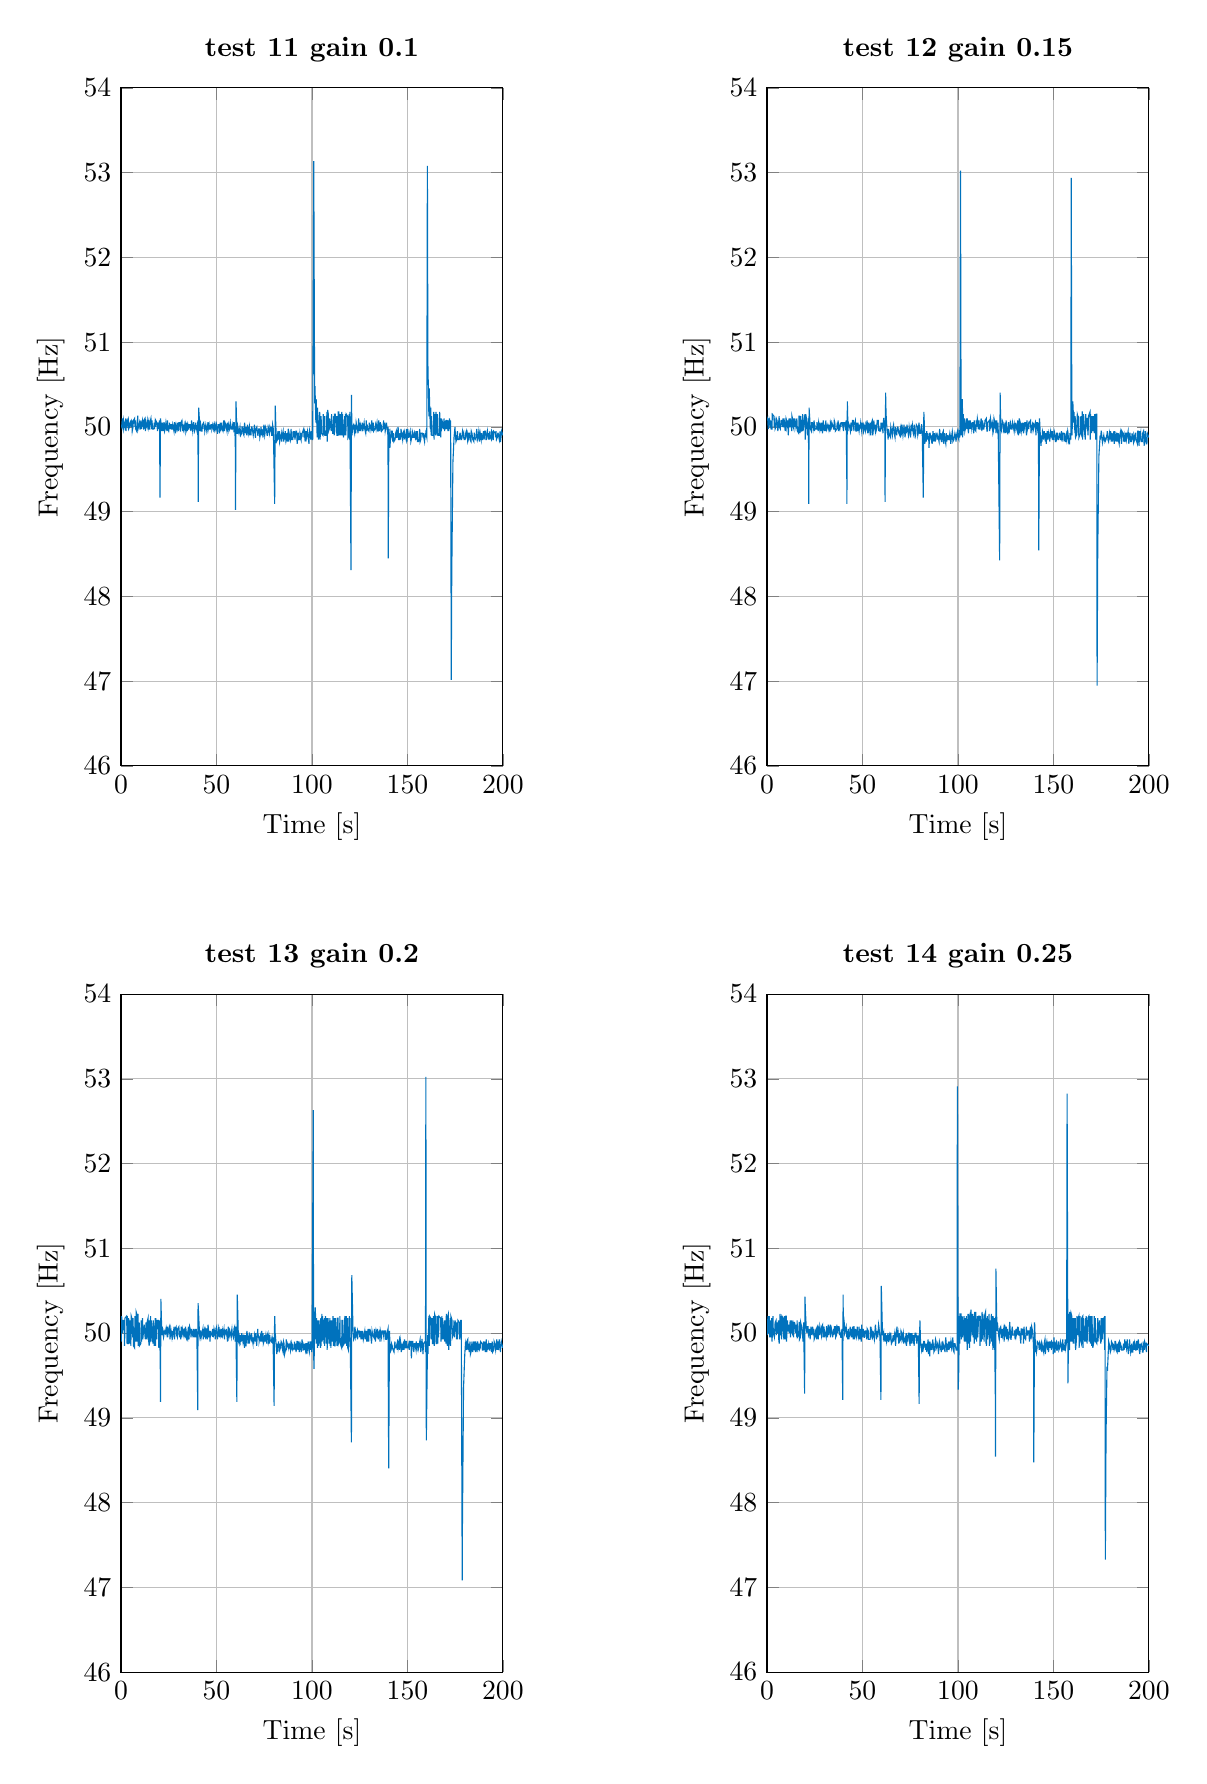
\begin{tikzpicture}

\begin{axis}[%
width=0.4\textwidth,
height=3.39in,
at={(0.953in,6.546in)},
scale only axis,
xmin=0,
xmax=200,
xlabel={Time [s]},
xmajorgrids,
ymin=46,
ymax=54,
ylabel={Frequency [Hz]},
ymajorgrids,
axis background/.style={fill=white},
title style={font=\bfseries},
title={test 11 gain 0.1}
]
\addplot [color=mycolor1,solid,forget plot]
  table[row sep=crcr]{%
0.0397	50.0250125062531\\
0.35946	50\\
0.6392	50.1002004008017\\
0.67912	50.0751126690035\\
1.19884	49.9750124937532\\
1.31886	50\\
1.35886	50.0751126690037\\
1.9984	50\\
2.51796	50.1002004008017\\
2.6379	49.9500499500496\\
2.79796	50.0500500500503\\
3.19774	50.0751126690034\\
3.35758	50.0250125062527\\
3.83724	50.0751126690034\\
3.99708	49.9750124937529\\
4.51698	50\\
4.63698	50.0500500500503\\
5.27656	50.075112669004\\
5.35646	50\\
5.7162	50.075112669004\\
5.87614	49.9500499500496\\
6.27612	50\\
6.47602	50.0751126690028\\
7.11554	50.1002004008011\\
7.27534	50\\
7.5552	50.075112669004\\
7.67508	49.9750124937529\\
8.19486	49.9500499500485\\
8.75462	50.1253132832088\\
8.79452	50.1253132832066\\
8.91436	49.9750124937529\\
9.67406	50.0500500500492\\
9.95398	49.9750124937529\\
10.03398	49.9750124937529\\
10.39374	50.075112669004\\
10.6735	49.9750124937529\\
11.27326	50.075112669004\\
11.83282	49.9750124937529\\
11.87284	49.9750124937529\\
11.95286	50.075112669004\\
12.55246	50.1002004008011\\
12.75224	49.9500499500507\\
13.19214	50.0500500500492\\
13.67188	49.9999999999988\\
13.99176	50.075112669004\\
14.39132	49.9999999999988\\
14.6313	50.0500500500514\\
14.95108	49.9750124937529\\
15.07112	49.9750124937529\\
15.19108	50.0500500500514\\
15.6708	50.1002004008011\\
16.11042	49.9750124937507\\
16.27044	50.0751126690017\\
16.43026	49.9750124937507\\
17.11016	49.9750124937507\\
17.43016	50.0500500500492\\
17.55008	49.9750124937507\\
17.83002	50.0500500500492\\
18.10986	50.0000000000011\\
18.22982	50.0751126690062\\
18.78932	50.0500500500537\\
19.06922	49.9500499500485\\
19.38918	50.0500500500537\\
19.54906	49.9750124937507\\
20.14886	50.0751126690062\\
20.4295	49.1642084562416\\
20.59172	49.8753117206996\\
20.67178	50.1002004008033\\
21.35202	49.9500499500529\\
21.5921	50.0500500500492\\
22.11194	49.9500499500485\\
22.43202	50.0500500500492\\
22.59188	50.0500500500537\\
22.83188	49.9500499500485\\
23.15192	49.9750124937507\\
23.51188	50.0500500500492\\
24.03188	49.9500499500485\\
24.35196	50.0751126690062\\
24.51182	49.9750124937507\\
24.99194	49.9500499500485\\
25.39192	50.0500500500537\\
25.67184	49.9750124937507\\
25.83188	50.0250125062532\\
26.31188	50.0250125062532\\
26.39188	49.9750124937507\\
26.87188	49.9750124937507\\
27.07192	50.0250125062532\\
27.71192	49.9500499500529\\
27.95196	50.0500500500492\\
28.07184	50.0500500500492\\
28.59186	49.9251123315022\\
28.712	49.9750124937507\\
28.87204	50.0250125062532\\
29.352	49.9750124937507\\
29.752	50.0500500500537\\
30.03188	49.9500499500485\\
30.31198	50.0500500500492\\
30.79198	50.0500500500537\\
31.07188	49.9500499500485\\
31.19198	49.9500499500485\\
31.35202	50.0500500500492\\
31.91206	50.0751126690017\\
32.27194	49.950049950044\\
32.552	50.0250125062532\\
32.792	49.9750124937463\\
33.11208	50.0250125062532\\
33.592	49.9500499500529\\
33.79208	50.0250125062532\\
34.15198	49.9750124937463\\
34.432	50.0500500500492\\
34.752	49.950049950044\\
35.0321	50.0250125062532\\
35.47202	49.9750124937463\\
35.55204	49.9750124937551\\
35.67206	50.0250125062532\\
36.23202	50.0250125062532\\
36.59206	49.9500499500529\\
36.79222	49.9999999999922\\
36.95216	50.0751126690106\\
37.55196	49.950049950044\\
37.9921	50.0500500500492\\
38.07204	50.0500500500492\\
38.51194	49.9500499500529\\
38.83198	49.9750124937463\\
39.11202	50.0500500500492\\
39.3119	50.0000000000011\\
39.792	49.950049950044\\
40.27208	50.0751126690017\\
40.43278	49.1159135559918\\
40.55468	49.7265042267554\\
40.67474	50.2260170768472\\
41.39432	49.950049950044\\
41.71452	50.0250125062532\\
41.8345	50.0000000000011\\
41.95454	49.950049950044\\
42.43486	49.950049950044\\
42.6349	50.0250125062532\\
43.27498	50.0500500500581\\
43.47486	49.9750124937551\\
43.67486	50.0250125062532\\
43.87488	49.9500499500529\\
44.39486	50.0250125062532\\
44.9148	49.9500499500529\\
45.51506	50.0500500500492\\
45.55502	50.0500500500581\\
45.71492	49.9750124937551\\
46.1549	50.0250125062532\\
46.3949	49.9750124937463\\
46.79496	49.9750124937551\\
47.03502	50.0250125062532\\
47.43506	50.0250125062532\\
47.555	49.9750124937463\\
47.99504	50.0250125062532\\
48.35492	49.9750124937463\\
48.71498	50.0250125062532\\
48.9949	49.9750124937551\\
49.27484	50.0250125062532\\
49.63478	49.9750124937463\\
49.99482	50.0250125062532\\
50.51488	49.9251123315066\\
50.59496	49.9251123314978\\
50.87506	50.0250125062532\\
51.35506	50.0250125062532\\
51.63512	49.9251123314978\\
51.9152	50.0500500500581\\
52.1951	49.9500499500529\\
52.59514	50.0500500500492\\
52.95498	49.9750124937463\\
53.39516	49.9500499500529\\
53.59528	50.0250125062532\\
53.7552	50.0751126690017\\
54.19506	49.9500499500529\\
54.31514	49.9750124937463\\
54.47516	50.0500500500492\\
54.87506	50.0250125062532\\
55.47502	49.950049950044\\
55.67508	50.0500500500492\\
56.1151	49.9750124937551\\
56.27514	50.0250125062532\\
56.75508	49.9750124937463\\
57.23504	50.0500500500581\\
57.35496	50.0250125062532\\
57.555	49.9750124937463\\
58.11508	49.9750124937463\\
58.31512	50.0250125062532\\
58.7551	49.9750124937463\\
59.03508	50.0500500500492\\
59.27494	50.0500500500492\\
59.83492	49.8504486540446\\
59.95622	49.0196078431405\\
60.23772	50.3018108651897\\
60.47688	50.0751126690017\\
60.67682	49.9251123314978\\
61.07722	49.9251123315066\\
61.19734	50.0000000000011\\
61.79774	49.9251123315066\\
62.31826	50.0000000000011\\
62.67848	49.9001996007944\\
63.159	49.9251123314978\\
63.3592	50.0000000000011\\
63.75948	50.0000000000011\\
63.95964	49.9251123314978\\
64.36006	49.9001996007944\\
64.72026	50.0500500500581\\
64.88018	50.0000000000099\\
65.2404	49.9251123315066\\
65.4406	49.9999999999922\\
65.88094	49.9001996007944\\
66.24134	50.0250125062532\\
66.68148	49.9251123315066\\
67.202	50.0000000000099\\
67.40212	49.9001996007944\\
67.60242	49.9750124937551\\
68.04296	49.9001996007944\\
68.32324	50.0000000000099\\
68.56326	50.0000000000099\\
69.08344	49.9251123315066\\
69.24366	49.9001996007944\\
69.76428	50.0000000000099\\
69.84428	50.0250125062532\\
70.36456	49.875311720704\\
70.44474	49.875311720704\\
70.56496	49.9750124937551\\
71.12536	50.0000000000099\\
71.64586	49.9001996008121\\
71.726	49.9001996008121\\
72.12644	49.9750124937374\\
72.40672	49.9750124937551\\
72.68702	49.8753117206863\\
73.08744	49.9251123314889\\
73.28762	49.9999999999922\\
73.72804	49.9001996007944\\
73.8482	49.9750124937551\\
74.36876	49.875311720704\\
74.80934	50.0250125062532\\
75.2496	49.9001996007944\\
75.40986	49.9251123315066\\
75.6501	50.0000000000099\\
76.05032	49.9750124937551\\
76.53078	49.9001996007944\\
76.69106	49.9001996007944\\
77.05144	50.0000000000099\\
77.33166	49.9750124937551\\
77.69198	49.9251123314889\\
77.97224	50.0000000000099\\
78.53242	49.950049950044\\
78.73254	50.0000000000099\\
78.85262	49.9001996007944\\
79.13312	49.9001996007944\\
79.37344	50.0250125062532\\
79.77354	49.9750124937551\\
80.4149	49.1642084562331\\
80.45558	49.0918016691218\\
80.77728	50.2512562814075\\
81.01642	50.0500500500581\\
81.41696	49.825610363717\\
81.93826	49.8504486540534\\
82.13864	49.9500499500618\\
82.45916	49.8504486540358\\
82.90016	49.9500499500618\\
83.10052	49.825610363717\\
83.90248	49.9251123315066\\
84.14288	49.825610363717\\
84.42368	49.9001996007944\\
84.90482	49.950049950044\\
85.18544	49.825610363717\\
85.386	49.9251123315066\\
85.66654	49.8504486540358\\
86.02734	49.9500499500618\\
86.3879	49.825610363717\\
86.70872	49.8504486540358\\
86.829	49.9251123315066\\
87.26984	49.825610363717\\
87.55054	49.9750124937551\\
87.9112	49.8256103637346\\
88.03152	49.9251123314889\\
88.71294	49.8504486540358\\
89.07356	49.9750124937374\\
89.11358	49.9500499500618\\
89.31388	49.8504486540358\\
89.91534	49.8504486540358\\
90.1158	49.950049950044\\
90.39632	49.8753117206863\\
90.75714	49.950049950044\\
91.1178	49.8504486540358\\
91.55868	49.9500499500618\\
91.95968	49.950049950044\\
92.24028	49.8007968127488\\
92.80168	49.9251123315066\\
92.88182	49.9251123315066\\
92.96196	49.8504486540358\\
93.60336	49.8504486540358\\
93.72366	49.9251123315066\\
94.32504	49.8504486540358\\
94.5256	49.9251123315066\\
94.72602	49.875311720704\\
94.84628	49.9251123315066\\
95.64762	49.9750124937551\\
95.80784	49.8753117206863\\
96.1686	49.9251123315066\\
96.4091	49.8256103637346\\
96.56962	49.8504486540358\\
96.89026	49.9500499500618\\
97.21084	49.875311720704\\
97.6917	49.9500499500618\\
97.85192	49.9251123315066\\
98.41324	49.8007968127488\\
98.4534	49.8504486540358\\
98.77406	49.950049950044\\
99.37526	49.8504486540534\\
99.65584	49.9500499500618\\
99.69588	49.9251123315066\\
100.17684	49.8504486540358\\
100.37732	49.8504486540358\\
100.93494	53.1349628055315\\
101.40496	50.2765208647467\\
101.56364	50.47955577991\\
102.04108	50.0500500500581\\
102.20052	50.3271263210937\\
102.71938	49.875311720704\\
102.91932	50.2260170768562\\
103.43868	49.8504486540358\\
104.03872	50.1756146512918\\
104.07858	50.1253132832043\\
104.23848	49.8504486540358\\
104.79856	50.1253132832043\\
104.95836	49.9251123315066\\
105.7179	49.9001996008121\\
105.91784	50.1504513540665\\
106.4775	49.9001996007944\\
106.67754	50.1253132832043\\
106.83738	49.9001996007944\\
107.59696	49.9001996007944\\
107.79698	50.1756146512739\\
107.99668	49.8256103637346\\
108.19686	50.2008032128538\\
108.55646	50.1504513540486\\
108.7162	49.9500499500618\\
109.07598	49.9750124937374\\
109.23588	50.1002004008078\\
110.07536	49.950049950044\\
110.27532	50.1504513540665\\
110.87478	49.9251123314889\\
111.2346	49.9251123315066\\
111.43454	50.1253132832222\\
111.6345	49.9001996007944\\
111.7945	50.1504513540665\\
112.19418	50.1504513540486\\
112.7937	49.9251123314889\\
112.99362	50.1253132832043\\
113.11348	49.9001996007944\\
113.51336	49.9001996007944\\
113.71346	50.1756146512918\\
114.11308	50.1756146512918\\
114.2728	49.9001996007944\\
114.87266	50.1504513540665\\
115.07246	49.9001996007944\\
115.63224	50.1756146512918\\
115.83192	49.9001996007944\\
116.0319	50.1504513540665\\
116.23176	49.9251123315066\\
116.55158	49.8753117206863\\
117.15146	50.1253132832222\\
117.3513	49.9001996007944\\
117.55126	50.1504513540665\\
117.7511	49.9001996007944\\
117.951	50.1504513540665\\
118.67072	50.1253132832043\\
118.87044	49.8753117206863\\
119.27034	49.9001996007944\\
119.4304	50.1504513540665\\
119.6701	49.8504486540358\\
119.87012	50.1756146512739\\
120.4309	48.3091787439662\\
120.67528	50.3778337531353\\
120.95434	49.9001996007944\\
121.31486	50.0000000000099\\
121.79498	50.0250125062532\\
122.11502	49.950049950044\\
122.31522	49.9251123315066\\
122.51538	50.0250125062532\\
122.95538	49.9251123315066\\
123.15544	50.0500500500581\\
123.3553	50.0250125062532\\
123.99534	49.9500499500618\\
124.07544	49.9251123314889\\
124.43542	50.1002004008078\\
124.71526	49.950049950044\\
124.95534	50.0500500500581\\
125.27534	49.950049950044\\
125.4354	50.0250125062532\\
126.07538	49.9750124937551\\
126.35542	50.0500500500581\\
126.47534	50.0250125062532\\
126.63534	49.950049950044\\
127.3153	50.0500500500581\\
127.63518	49.9750124937551\\
128.1555	49.9251123314889\\
128.35564	50.025012506271\\
128.4356	50.0751126690017\\
128.71552	49.950049950044\\
128.95556	50.025012506271\\
129.1955	49.9750124937551\\
129.8356	49.950049950044\\
129.99562	50.0500500500403\\
130.39548	49.9750124937196\\
130.55552	50.025012506271\\
130.83548	49.9750124937196\\
131.31542	50.0751126690017\\
131.47526	50.025012506271\\
131.59528	49.950049950044\\
132.11556	50.0500500500403\\
132.31546	49.950049950044\\
132.95548	49.9750124937196\\
133.31558	50.025012506271\\
133.59554	49.9750124937196\\
134.07556	50.0500500500759\\
134.47534	49.9500499500086\\
134.63546	49.950049950044\\
134.99552	50.0751126690017\\
135.23542	49.950049950044\\
135.79548	50.0500500500759\\
135.83544	50.0500500500759\\
136.0753	49.9750124937551\\
136.43528	50.0000000000099\\
136.47528	49.950049950044\\
137.27566	49.9750124937196\\
137.51554	50.0751126690017\\
137.67544	49.9750124937551\\
138.1155	50.0500500500403\\
138.3554	49.950049950044\\
138.91564	50.0250125062355\\
138.9956	50.0500500500403\\
139.51548	49.950049950044\\
139.79562	50.0000000000099\\
139.9577	48.4496124031336\\
140.16232	49.554013875098\\
140.36308	49.9750124937551\\
140.8049	49.7512437810962\\
141.32654	49.9251123314889\\
141.6872	49.8753117206687\\
141.80744	49.9500499500795\\
142.04778	49.9500499500795\\
142.2482	49.825610363717\\
142.68906	49.9251123315244\\
142.8895	49.825610363717\\
143.53092	49.8504486540358\\
143.81158	49.9251123315244\\
144.13214	49.9500499500795\\
144.25234	49.875311720704\\
144.61304	49.875311720704\\
145.09376	50.0000000000099\\
145.2539	49.9500499500795\\
145.37412	49.8504486540358\\
145.85536	49.8504486540358\\
146.0558	49.9251123315244\\
146.4164	49.8504486540358\\
146.61686	49.9750124937551\\
147.4585	49.8504486540711\\
147.65898	49.9251123315244\\
148.09988	49.9500499500795\\
148.26014	49.8504486540358\\
148.5809	49.9251123315244\\
149.30248	49.8504486540358\\
149.50284	49.9750124937906\\
149.78328	49.8256103637522\\
150.14406	49.9750124937551\\
150.6651	49.8753117206687\\
150.7854	49.875311720704\\
151.18628	49.9251123314889\\
151.42674	49.950049950044\\
151.78748	49.825610363717\\
152.26838	49.875311720704\\
152.54892	49.950049950044\\
152.86954	49.9251123314889\\
152.98978	49.8753117206687\\
153.39062	49.875311720704\\
153.67118	49.9251123315244\\
154.07198	49.8753117206687\\
154.47274	49.9500499500795\\
154.67306	49.8504486540358\\
155.11404	49.9500499500795\\
155.27428	49.825610363717\\
155.87578	49.825610363717\\
156.31688	49.950049950044\\
156.39698	49.9750124937551\\
156.63742	49.825610363717\\
156.99836	49.8504486540358\\
157.19882	49.9251123315244\\
157.88014	49.9251123315244\\
158.20074	49.8753117206687\\
158.321	49.9251123314889\\
158.56144	49.875311720704\\
158.9623	49.825610363717\\
159.28318	49.9251123314889\\
159.4836	49.875311720704\\
159.64396	49.9251123315244\\
160.12486	49.875311720704\\
160.4411	53.0785562632772\\
160.71476	50.735667174051\\
161.23058	50.1253132832222\\
161.3898	50.4540867810401\\
161.98774	49.9750124937551\\
162.18736	50.2260170768562\\
162.38698	49.9001996007767\\
162.62676	50.1253132832222\\
162.78668	49.9001996008121\\
163.54608	49.9001996007767\\
163.7461	50.1756146512739\\
163.94582	49.8504486540358\\
164.14592	50.1504513540844\\
164.7455	49.9001996007767\\
164.94542	50.1756146512739\\
165.545	49.9001996007767\\
165.70502	50.1504513540844\\
165.90476	49.9001996008121\\
166.66416	49.9001996008121\\
166.86426	50.1756146512739\\
166.94398	50.1253132832222\\
167.46376	49.875311720704\\
167.66396	50.1002004008078\\
168.02352	49.9999999999744\\
168.38338	50.0500500500759\\
168.82314	49.9750124937551\\
169.18302	50.1002004008078\\
169.46272	49.950049950044\\
169.9825	50.0751126690017\\
170.30234	49.9750124937196\\
170.46234	50.0751126690017\\
170.7021	50.0751126690017\\
171.22184	49.9500499500795\\
171.50174	50.0751126690017\\
171.6216	49.950049950044\\
171.9815	50.1002004008078\\
172.4211	49.9750124937551\\
172.62108	50.0751126690017\\
172.94342	47.0145745180979\\
173.1963	48.2392667631444\\
173.80778	49.5785820525702\\
174.45122	49.9001996008121\\
174.4913	49.9001996007767\\
174.8919	49.9999999999744\\
175.05206	49.9251123315244\\
175.41282	49.8256103637522\\
175.73364	49.8504486540358\\
176.17456	49.9500499500795\\
176.2947	49.9001996008121\\
176.37488	49.8504486540358\\
177.09666	49.8504486540358\\
177.45748	49.9251123315244\\
177.6178	49.9251123315244\\
177.9785	49.8504486540358\\
178.37934	49.8504486540711\\
178.7	49.9251123315244\\
178.86024	49.950049950044\\
179.18074	49.9001996007767\\
179.46122	49.9251123314889\\
179.66164	49.8504486540358\\
180.22298	49.8504486540358\\
180.50362	49.9251123315244\\
180.82414	49.950049950044\\
181.0244	49.9001996007767\\
181.30492	49.9251123315244\\
181.58554	49.825610363717\\
181.90656	49.8504486540711\\
182.0669	49.9251123315244\\
182.50784	49.9251123315244\\
182.78836	49.8504486540358\\
183.26942	49.825610363717\\
183.42984	49.9500499500795\\
183.7904	49.9251123315244\\
184.23136	49.8504486540358\\
184.79274	49.8256103637522\\
184.9532	49.9251123315244\\
185.07338	49.9251123315244\\
185.1936	49.875311720704\\
185.83496	49.8504486540358\\
186.2759	49.9750124937551\\
186.7967	49.8504486540711\\
187.07728	49.875311720704\\
187.39802	49.950049950044\\
187.55824	49.9251123315244\\
187.75874	49.825610363717\\
188.11958	49.9251123315244\\
188.6406	49.8504486540358\\
188.84106	49.9251123314889\\
189.04142	49.8504486540358\\
189.36226	49.8504486540358\\
189.80332	49.9500499500795\\
190.16398	49.8504486540358\\
190.44452	49.9500499500795\\
190.92558	49.950049950044\\
191.12592	49.8504486540358\\
191.28634	49.8504486540358\\
191.88792	49.950049950044\\
192.40874	49.8504486540358\\
192.52902	49.9251123314889\\
192.80962	49.8504486540358\\
193.17038	49.950049950044\\
193.3707	49.875311720704\\
193.9318	49.8504486540358\\
194.13232	49.950049950044\\
194.53302	49.9251123314889\\
194.73344	49.8504486540358\\
194.9741	49.8504486540358\\
195.09434	49.950049950044\\
196.05616	49.9251123315244\\
196.09622	49.8753117206687\\
196.37676	49.950049950044\\
196.61714	49.8504486540358\\
197.0581	49.875311720704\\
197.33866	49.9251123315244\\
197.49894	49.9251123315244\\
198.10008	49.8504486540358\\
198.54114	49.9500499500795\\
198.66136	49.825610363717\\
198.7416	49.825610363717\\
199.34294	49.950049950044\\
199.94418	49.9001996007767\\
};
\end{axis}

\begin{axis}[%
width=0.4\textwidth,
height=3.39in,
at={(4.183in,6.546in)},
scale only axis,
xmin=0,
xmax=200,
xlabel={Time [s]},
xmajorgrids,
ymin=46,
ymax=54,
ylabel={Frequency [Hz]},
ymajorgrids,
axis background/.style={fill=white},
title style={font=\bfseries},
title={test 12  gain 0.15}
]
\addplot [color=mycolor1,solid,forget plot]
  table[row sep=crcr]{%
0.03974	50.0751126690035\\
0.35934	50.1002004008017\\
0.63908	49.9750124937532\\
0.75902	50.1002004008015\\
0.87888	50\\
1.39852	50.0751126690037\\
1.83812	50\\
1.9181	50.0751126690037\\
2.1179	49.9750124937529\\
2.63748	49.9750124937529\\
2.7574	50.150451354062\\
3.63632	50.1253132832077\\
3.7561	50\\
3.876	50.1002004008011\\
4.2357	49.9750124937529\\
4.63546	50\\
4.83522	50.1002004008022\\
5.2748	50.075112669004\\
5.67464	49.9500499500496\\
6.27434	50.1002004008022\\
6.35418	50.1253132832077\\
6.47402	50\\
6.9537	49.9750124937529\\
7.3535	50.075112669004\\
7.6332	50.075112669004\\
7.9928	49.9999999999988\\
8.35252	50.1002004008011\\
8.51232	49.9999999999988\\
8.79212	49.9999999999988\\
8.91202	50.1002004008033\\
9.51154	49.9500499500485\\
9.95134	50.1002004008011\\
10.27098	50.075112669004\\
10.3909	49.9999999999988\\
10.99076	50.075112669004\\
11.15068	49.9001996007988\\
11.55066	50.1002004008011\\
11.71048	49.9999999999988\\
11.99032	49.9999999999988\\
12.19012	50.1002004008011\\
12.94948	49.9500499500507\\
13.06948	50.1253132832088\\
13.30918	50.1002004008033\\
13.74868	49.9999999999988\\
14.0686	49.9750124937529\\
14.14856	50.1002004008011\\
14.38838	49.9999999999988\\
14.5482	50.1002004008033\\
15.1076	49.9999999999988\\
15.62728	50.1002004008011\\
15.90698	49.9500499500507\\
16.58664	49.9251123315022\\
16.74664	50.1253132832088\\
17.1462	50.1253132832043\\
17.306	49.9251123315022\\
17.50608	50.1253132832043\\
18.06558	49.9500499500485\\
18.10562	49.9500499500485\\
18.66534	50.150451354062\\
18.74512	50.1002004008033\\
18.86504	49.9500499500485\\
19.86434	50.150451354062\\
19.98414	49.9001996007988\\
20.02422	49.8504486540402\\
20.26428	50.150451354062\\
20.66398	50.1002004008033\\
21.14368	49.9001996007988\\
21.70358	50.1002004008033\\
21.86482	49.0918016691218\\
22.02634	50.2260170768472\\
22.50584	50.0500500500537\\
22.74576	49.9750124937507\\
23.18564	49.9500499500529\\
23.3857	50.0500500500492\\
23.78566	50.0500500500492\\
24.14554	49.9750124937507\\
24.66546	50.0751126690062\\
24.90526	49.9500499500485\\
25.06532	50.0250125062532\\
25.26528	49.9750124937507\\
25.98508	49.9750124937507\\
26.18508	50.0500500500537\\
26.22504	50.0500500500492\\
26.7848	49.9500499500485\\
26.86486	49.9750124937507\\
27.06484	50.0500500500492\\
27.58468	49.9750124937551\\
27.78466	50.0500500500537\\
28.26456	49.9500499500485\\
28.66454	50.0500500500537\\
28.7445	50.0250125062532\\
29.02448	49.9251123315022\\
29.46454	50.0751126690017\\
29.90452	49.9500499500529\\
30.02456	50.0250125062532\\
30.38446	49.9500499500485\\
30.82442	50.0751126690017\\
30.98434	49.9500499500485\\
31.18444	50.0250125062532\\
31.34442	49.9750124937507\\
31.86454	50.0250125062532\\
32.30442	49.9750124937551\\
32.42446	50.0250125062532\\
32.70444	49.9500499500529\\
33.06456	49.9500499500529\\
33.22464	50.0500500500492\\
33.74454	49.9999999999922\\
33.9445	50.0500500500492\\
34.30428	50.0250125062532\\
34.90418	49.9750124937551\\
34.9842	49.9750124937463\\
35.2241	50.0751126690106\\
35.54388	50.0500500500492\\
35.78376	49.950049950044\\
36.54374	49.9750124937551\\
36.74372	50.0500500500492\\
37.02362	49.9750124937463\\
37.22356	50.0751126690106\\
37.46338	49.950049950044\\
37.62352	50.0250125062532\\
38.14336	49.9750124937463\\
38.58334	50.0500500500581\\
38.70328	50.0000000000011\\
38.9432	50.0500500500492\\
39.46292	50.0500500500492\\
39.90274	49.9750124937463\\
40.06282	49.950049950044\\
40.18286	50.0500500500492\\
40.58276	50.0500500500492\\
40.98254	49.9999999999922\\
41.4625	50.0751126690106\\
41.78266	49.3827160493808\\
41.82316	49.0918016691218\\
42.06494	50.3018108651897\\
42.42404	49.9500499500529\\
42.62408	50.0500500500581\\
43.02412	50.0250125062532\\
43.66418	49.950049950044\\
43.94428	50.0500500500581\\
44.30422	49.950049950044\\
44.74418	50.0751126690017\\
45.144	50.0751126690106\\
45.50378	49.9500499500529\\
45.62382	50.0250125062532\\
46.26368	50.0751126690017\\
46.50356	49.950049950044\\
46.86372	49.950049950044\\
47.10374	50.0500500500492\\
47.4236	49.950049950044\\
47.6237	50.0500500500492\\
48.22356	49.9500499500529\\
48.5837	50.0250125062532\\
48.62368	49.9750124937463\\
49.06374	50.0500500500492\\
49.58378	49.9500499500529\\
49.86394	50.0250125062532\\
49.90392	50.0500500500492\\
50.14374	50.0000000000011\\
50.50354	50.0250125062532\\
50.62352	49.950049950044\\
51.3838	50.0250125062532\\
51.58378	49.9500499500529\\
51.86386	49.9750124937551\\
52.26382	50.0500500500492\\
52.42368	50.0751126690017\\
52.7035	49.9251123315066\\
53.14376	50.0500500500492\\
53.50354	49.950049950044\\
54.06366	50.0500500500581\\
54.22356	49.950049950044\\
54.34372	49.9001996008032\\
54.7439	50.0500500500492\\
55.1038	50.0751126690017\\
55.38374	49.9001996008032\\
55.74376	49.9750124937551\\
55.94374	50.0751126690106\\
56.10356	50.0250125062532\\
56.7036	49.9500499500529\\
56.82364	50.0250125062532\\
57.10362	49.950049950044\\
57.42366	49.9750124937551\\
57.70366	50.0751126690017\\
58.26344	50.0751126690017\\
58.46342	49.950049950044\\
58.58348	50.0000000000011\\
59.02356	49.9500499500529\\
59.50376	49.950049950044\\
59.70378	50.0500500500492\\
60.02366	49.9750124937463\\
60.34374	50.0500500500492\\
60.70364	49.9251123314978\\
61.06384	50.1002004007989\\
61.1437	50.1002004007989\\
61.70356	49.9500499500529\\
61.82436	49.1159135559918\\
62.1057	50.4032258064463\\
62.34436	50.1504513540665\\
62.9441	49.9251123314978\\
63.0242	49.9750124937551\\
63.42476	49.8504486540358\\
63.62508	49.9750124937551\\
64.14558	49.9001996007944\\
64.66624	49.8753117206863\\
64.82648	49.9999999999922\\
65.42712	49.9251123314889\\
65.66742	49.9001996007944\\
65.7876	49.9750124937551\\
66.26786	50.0250125062532\\
66.62804	49.9251123315066\\
67.02848	49.8753117206863\\
67.309	50.0000000000099\\
67.9095	49.9001996007944\\
67.94958	49.9251123315066\\
68.47	50.0000000000099\\
68.55	50.0000000000099\\
69.03036	49.9251123314889\\
69.51092	49.9001996008121\\
69.71118	49.9750124937551\\
69.99136	50.0000000000099\\
70.15144	49.9001996007944\\
70.55208	49.9251123314889\\
70.67218	50.0250125062532\\
71.19248	49.9001996007944\\
71.6729	50.0000000000099\\
71.7129	50.0250125062532\\
72.31316	49.875311720704\\
72.59356	50.0000000000099\\
72.95392	49.9251123315066\\
73.31414	50.0250125062532\\
73.55414	49.9750124937551\\
74.07458	49.9001996008121\\
74.19476	49.9251123314889\\
74.43498	50.0000000000099\\
75.19558	49.875311720704\\
75.39594	50.0000000000099\\
75.47596	50.0250125062532\\
75.676	49.950049950044\\
76.11622	50.0250125062532\\
76.55642	49.9251123314889\\
76.87686	49.9001996007944\\
77.1172	50.0250125062532\\
77.27712	49.9750124937551\\
77.75758	49.9001996007944\\
77.9178	49.9251123315066\\
78.198	50.0250125062532\\
78.83832	50.0000000000099\\
78.95844	49.9001996007944\\
79.1987	49.9251123314889\\
79.55898	50.0500500500403\\
79.79898	49.9999999999922\\
79.99914	49.9251123315066\\
80.47954	49.9251123314889\\
80.92006	50.0250125062532\\
81.00004	50.0250125062532\\
81.2801	49.950049950044\\
81.8411	49.1642084562502\\
82.1229	50.1756146512739\\
82.28246	50.10020040079\\
82.64284	49.8007968127488\\
83.16422	49.9251123314889\\
83.40482	49.825610363717\\
83.6454	49.9500499500618\\
83.96602	49.8504486540358\\
84.2066	49.9251123315066\\
84.76778	49.825610363717\\
84.80792	49.7512437810962\\
85.24936	49.9251123315066\\
85.40964	49.9251123315066\\
86.01076	49.8504486540358\\
86.25138	49.9001996008121\\
86.49196	49.8007968127488\\
86.933	49.950049950044\\
87.25356	49.8504486540358\\
87.37392	49.8256103637346\\
87.57444	49.9251123315066\\
88.17596	49.825610363717\\
88.45668	49.9251123315066\\
88.53682	49.9251123315066\\
89.05776	49.8753117206863\\
89.13796	49.8504486540358\\
89.41864	49.9001996008121\\
90.10036	49.8256103637346\\
90.34092	49.9500499500618\\
90.38096	49.9750124937551\\
90.82186	49.8504486540358\\
91.06248	49.9251123315066\\
91.30306	49.825610363717\\
91.70412	49.825610363717\\
91.90466	49.9251123315066\\
92.30568	49.9500499500618\\
92.58632	49.8007968127488\\
92.86702	49.9251123315066\\
93.22776	49.8504486540358\\
93.62882	49.8007968127488\\
93.86946	49.9251123315066\\
94.19022	49.8256103637346\\
94.23036	49.9001996007944\\
94.79168	49.9001996007944\\
94.83176	49.8504486540358\\
95.353	49.8504486540358\\
95.75408	49.9251123315066\\
95.95448	49.9001996007944\\
96.19514	49.8007968127488\\
96.59624	49.875311720704\\
97.03718	49.950049950044\\
97.19742	49.9251123315066\\
97.31766	49.825610363717\\
97.87912	49.8504486540358\\
98.40034	49.9251123314889\\
98.64092	49.9001996007944\\
99.0019	49.8256103637346\\
99.08216	49.8504486540358\\
99.44302	49.9251123315066\\
99.76366	49.950049950044\\
100.04416	49.8753117206863\\
100.4451	49.8504486540358\\
100.5654	49.9251123315066\\
101.00622	49.875311720704\\
101.32364	53.022269353138\\
101.59684	50.4286434694935\\
101.71612	49.9001996007944\\
102.31462	50.3271263210757\\
102.43414	49.875311720704\\
102.83322	50.1504513540665\\
102.91306	49.950049950044\\
103.51244	50.1002004008078\\
103.63232	49.950049950044\\
104.11212	49.9999999999922\\
104.63176	50.1002004008078\\
104.75164	49.9750124937551\\
104.87156	50.10020040079\\
105.47122	49.9251123314889\\
105.75112	50.0751126690195\\
105.91104	49.9750124937551\\
106.43082	50.0751126690017\\
106.67066	49.9750124937551\\
106.87064	50.0500500500581\\
107.23046	49.9750124937551\\
107.59048	50.0500500500581\\
107.91046	50.0500500500581\\
108.27036	49.9251123315066\\
108.55034	50.0751126690017\\
108.71022	49.9750124937551\\
109.39008	49.9500499500618\\
109.5101	50.0751126690017\\
109.78986	49.9999999999922\\
110.14978	50.1002004008078\\
110.30956	50.0751126690017\\
110.6693	49.9750124937551\\
111.02926	50.0751126690017\\
111.14918	49.9750124937374\\
111.54914	49.9750124937551\\
112.14888	50.10020040079\\
112.50856	49.950049950044\\
112.86852	50.0751126690017\\
113.14836	49.9750124937551\\
113.5482	49.9750124937551\\
113.9082	50.0500500500581\\
114.02812	49.9999999999922\\
114.14806	50.0751126690017\\
114.82758	50.1002004008078\\
115.14742	49.9500499500618\\
115.34734	49.950049950044\\
115.50738	50.0500500500581\\
116.38722	50.0751126690195\\
116.50718	49.950049950044\\
117.027	50.10020040079\\
117.18676	50.0751126690017\\
117.3866	49.9999999999922\\
117.94632	50.0500500500581\\
118.3062	49.9251123315066\\
118.54622	49.950049950044\\
118.86634	50.1002004008078\\
119.10606	50.0751126690195\\
119.46568	49.9750124937551\\
119.66564	50.0751126690017\\
119.94552	49.9251123314889\\
120.30552	50.0751126690017\\
120.42544	49.9750124937551\\
120.90536	49.9251123314889\\
121.02542	50.0500500500581\\
121.82672	48.4261501210741\\
122.06986	50.4032258064463\\
122.10954	50.3778337531533\\
122.42814	49.9750124937551\\
122.82814	49.950049950044\\
123.18808	50.0751126690195\\
123.62802	50.0500500500581\\
123.98792	49.950049950044\\
124.02796	49.9251123315066\\
124.62796	50.0500500500403\\
124.908	49.9251123314889\\
125.22822	50.0751126690017\\
125.50808	49.950049950044\\
126.02792	49.9251123315066\\
126.38806	50.0500500500581\\
126.468	50.0500500500403\\
126.748	49.9251123315066\\
127.26808	50.0250125062532\\
127.468	49.9750124937551\\
127.708	50.0250125062532\\
127.98794	49.9750124937551\\
128.34806	49.9750124937551\\
128.62804	50.0500500500759\\
129.38814	49.9500499500086\\
129.58826	50.025012506271\\
129.94832	49.9750124937196\\
130.30824	50.0500500500759\\
130.42816	50.0000000000099\\
131.02802	49.950049950044\\
131.26808	50.0751126690374\\
131.668	49.9001996007767\\
132.06808	50.1002004008078\\
132.34798	49.9251123314889\\
132.78796	50.025012506271\\
133.148	49.950049950044\\
133.58816	50.0500500500403\\
133.94808	49.950049950044\\
134.14808	50.0500500500759\\
134.34806	49.9251123315244\\
134.70814	49.9750124937196\\
134.98816	50.0500500500759\\
135.42808	50.0500500500403\\
135.78804	49.9251123314889\\
135.86816	49.9001996008121\\
136.1482	50.0751126690017\\
136.42806	49.9750124937196\\
136.86814	50.025012506271\\
137.0681	49.9750124937551\\
137.34812	50.0500500500759\\
137.988	50.0751126690017\\
138.26792	49.9251123314889\\
138.348	49.950049950044\\
138.94826	50.025012506271\\
139.22816	49.9750124937551\\
139.50816	50.0500500500403\\
139.54812	50.025012506271\\
139.62808	49.9750124937551\\
140.5081	50.0500500500759\\
140.78796	49.9251123314889\\
140.82802	49.9001996008121\\
141.1083	50.0500500500403\\
141.58808	50.0500500500759\\
141.86802	49.9251123314889\\
142.14826	50.0500500500759\\
142.30904	48.5436893203843\\
142.71436	50.1002004007721\\
143.23472	49.8504486540358\\
143.4755	49.7760079641708\\
143.83674	49.9001996007767\\
144.03722	49.8256103637522\\
144.27772	49.9500499500795\\
144.55824	49.9251123315244\\
144.83886	49.8504486540358\\
145.19976	49.950049950044\\
145.80118	49.8256103637522\\
146.00176	49.9251123315244\\
146.20224	49.8007968127311\\
146.40282	49.8504486540358\\
146.72354	49.950049950044\\
147.04416	49.8504486540358\\
147.44518	49.9251123315244\\
148.12672	49.825610363717\\
148.24708	49.9251123315244\\
148.48756	49.950049950044\\
148.68792	49.8753117206687\\
149.12874	49.9500499500795\\
149.40928	49.8504486540358\\
149.52958	49.950049950044\\
149.7299	49.8504486540358\\
150.21096	49.8504486540358\\
150.41146	49.950049950044\\
150.93268	49.9001996008121\\
151.09306	49.825610363717\\
151.41404	49.825610363717\\
151.69478	49.9251123315244\\
152.09574	49.9251123315244\\
152.29614	49.8504486540358\\
152.61684	49.8504486540358\\
153.21834	49.9251123315244\\
153.2985	49.9251123315244\\
153.65928	49.8504486540358\\
153.98012	49.8504486540358\\
154.1806	49.950049950044\\
154.5413	49.825610363717\\
154.74184	49.9251123314889\\
155.42364	49.9251123315244\\
155.58394	49.825610363717\\
155.86474	49.9251123315244\\
156.3859	49.8256103637522\\
156.46614	49.825610363717\\
156.78702	49.9001996008121\\
157.02764	49.8504486540358\\
157.46874	49.950049950044\\
157.62894	49.9251123314889\\
158.07004	49.8007968127664\\
158.43132	49.8007968127311\\
158.67208	49.9251123314889\\
159.11288	49.8504486540358\\
159.31088	52.9380624669166\\
159.58352	50.5050505050413\\
159.74262	49.9001996008121\\
160.14134	50.3018108652257\\
160.61952	50.0500500500403\\
160.73926	50.1756146512739\\
161.25854	49.9251123315244\\
161.37852	50.1253132832222\\
161.57836	49.875311720704\\
161.97822	49.9001996007767\\
162.49796	50.1504513540844\\
162.81784	50.1253132832222\\
163.01758	49.9001996008121\\
163.2176	50.1253132832222\\
163.37746	49.875311720704\\
164.13708	49.9251123314889\\
164.33716	50.1253132832222\\
164.89676	49.875311720704\\
165.05692	50.1756146513097\\
165.09678	50.1756146512739\\
165.25656	49.8504486540358\\
165.77652	50.1504513540486\\
166.33594	49.9251123314889\\
166.69568	49.8504486540358\\
166.89574	50.1504513540844\\
167.0555	49.9750124937551\\
167.21544	50.1002004008078\\
167.5751	50.1002004008078\\
168.13454	49.9001996007767\\
168.21466	49.9750124937551\\
168.33456	50.1253132832222\\
169.1338	50.1756146512739\\
169.2937	49.8504486540358\\
169.45388	50.1504513540486\\
169.97322	49.9251123314889\\
170.1731	50.1253132832222\\
170.6926	49.950049950044\\
170.89266	50.1253132832222\\
171.41208	49.9251123314889\\
171.65198	50.1504513540844\\
172.17156	49.8504486540358\\
172.37156	50.1504513540844\\
172.69124	50.1504513540486\\
172.8544	46.9483568075194\\
173.18918	48.5201358563689\\
173.79948	49.6524329691858\\
174.44266	49.9001996008121\\
174.6431	49.8504486540358\\
175.00386	49.950049950044\\
175.08396	49.950049950044\\
175.52478	49.8504486540358\\
175.6852	49.875311720704\\
175.7654	49.825610363717\\
176.36716	49.9001996008121\\
176.8082	49.825610363717\\
176.92854	49.875311720704\\
177.04886	49.825610363717\\
177.53032	49.8504486540358\\
178.13176	49.9251123315244\\
178.2119	49.9500499500795\\
178.53256	49.8504486540358\\
178.89342	49.825610363717\\
179.33478	49.9251123314889\\
179.77564	49.8504486540358\\
179.93598	49.950049950044\\
180.05614	49.9251123314889\\
180.25664	49.825610363717\\
180.73786	49.9251123315244\\
180.93838	49.825610363717\\
181.65996	49.950049950044\\
181.86042	49.8007968127664\\
181.9407	49.825610363717\\
182.1412	49.950049950044\\
182.82288	49.825610363717\\
183.10376	49.9251123314889\\
183.1839	49.9251123314889\\
183.46462	49.825610363717\\
183.9059	49.9251123314889\\
184.18652	49.825610363717\\
184.42716	49.8007968127311\\
184.66792	49.9001996008121\\
185.18914	49.950049950044\\
185.6302	49.8007968127664\\
185.83078	49.950049950044\\
186.47224	49.9251123314889\\
186.67268	49.8256103637522\\
187.07374	49.9001996008121\\
187.4747	49.8256103637522\\
187.55494	49.825610363717\\
187.83574	49.9251123315244\\
188.15644	49.9251123315244\\
188.27666	49.8504486540358\\
189.1187	49.950049950044\\
189.3591	49.8504486540358\\
189.47948	49.8007968127311\\
190.0009	49.9251123314889\\
190.08106	49.9251123315244\\
190.44192	49.8256103637522\\
190.76282	49.825610363717\\
191.204	49.9251123315244\\
191.28414	49.9001996008121\\
191.88558	49.825610363717\\
192.08616	49.9001996008121\\
192.52722	49.8504486540358\\
192.96834	49.9251123315244\\
193.12862	49.9251123315244\\
193.24886	49.8504486540358\\
193.9708	49.8007968127311\\
194.17132	49.950049950044\\
194.49186	49.950049950044\\
194.8528	49.7760079641708\\
195.05332	49.9500499500795\\
195.1735	49.8504486540358\\
195.69458	49.9251123314889\\
195.895	49.8256103637522\\
196.53658	49.825610363717\\
196.73714	49.9251123315244\\
197.1781	49.950049950044\\
197.45866	49.8007968127664\\
197.49882	49.7760079641708\\
198.10068	49.9500499500795\\
198.54154	49.8007968127311\\
198.94278	49.8007968127311\\
199.1433	49.9251123315244\\
199.9452	49.875311720704\\
};
\end{axis}

\begin{axis}[%
width=0.4\textwidth,
height=3.39in,
at={(0.953in,2.015in)},
scale only axis,
xmin=0,
xmax=200,
xlabel={Time [s]},
xmajorgrids,
ymin=46,
ymax=54,
ylabel={Frequency [Hz]},
ymajorgrids,
axis background/.style={fill=white},
title style={font=\bfseries},
title={test 13  gain 0.2}
]
\addplot [color=mycolor1,solid,forget plot]
  table[row sep=crcr]{%
0.03966	50.1002004008016\\
0.11956	49.9001996007984\\
0.3195	50.2008032128514\\
0.8386	50\\
0.99842	50.150451354062\\
1.63762	50.1504513540623\\
1.8373	49.850448654038\\
1.91752	49.9251123315028\\
2.03742	50.1756146512795\\
2.95682	50.200803212851\\
3.15656	49.8753117206985\\
3.27662	50.2008032128516\\
3.47628	49.875311720698\\
3.83598	49.8753117206985\\
3.99604	50.1756146512795\\
4.51544	49.8753117206985\\
4.63556	50.1504513540631\\
5.15504	49.850448654038\\
5.35526	50.2008032128516\\
5.6751	50.1756146512795\\
6.11434	49.9500499500496\\
6.31424	50.1756146512795\\
6.5142	49.850448654038\\
7.11412	49.825610363728\\
7.27428	50.2008032128516\\
7.7539	49.9001996007977\\
7.91384	50.2512562814075\\
8.23342	50.226017076845\\
8.43306	49.9001996007988\\
8.87276	50.2260170768472\\
9.03256	49.8504486540358\\
9.5123	50.1253132832088\\
9.67212	49.850448654038\\
10.352	49.8753117206974\\
10.55208	50.150451354062\\
10.71186	49.9001996007988\\
11.23158	50.1756146512806\\
11.27144	50.1253132832066\\
11.39128	49.9251123315022\\
12.15086	50.1002004008033\\
12.51058	49.9750124937529\\
12.75052	49.9251123315022\\
13.11054	50.1253132832066\\
13.51022	49.9251123315022\\
13.6302	50.1253132832088\\
14.14984	50.1756146512806\\
14.26962	49.9500499500485\\
14.74944	49.850448654038\\
14.86956	50.150451354062\\
14.98934	49.8753117206974\\
15.50942	50.2008032128516\\
15.66908	49.9001996007988\\
15.82922	50.1504513540642\\
16.70848	49.8753117206996\\
16.8686	50.150451354062\\
17.38822	49.8504486540358\\
17.90804	50.1756146512828\\
18.06796	49.8504486540402\\
18.10808	49.9001996007988\\
18.22808	50.1756146512784\\
18.7476	49.9251123315022\\
18.86762	50.150451354062\\
19.58738	50.150451354062\\
19.78724	49.8256103637258\\
20.2271	50.150451354062\\
20.62692	49.4804552201868\\
20.66734	49.1883915395978\\
20.86892	50.4032258064508\\
21.22734	50.1002004008033\\
21.5868	49.9750124937507\\
21.86674	50.0250125062532\\
22.26666	49.9500499500485\\
22.46666	49.9750124937507\\
22.66672	50.0250125062532\\
23.14676	49.9999999999966\\
23.54672	50.0500500500492\\
23.70664	49.9999999999966\\
24.22648	50.0751126690062\\
24.42634	49.9500499500485\\
24.94636	50.0500500500492\\
25.26616	50.0751126690062\\
25.58596	49.9750124937507\\
25.66602	49.9251123315022\\
26.06616	50.0500500500492\\
26.22602	50.0250125062532\\
26.66606	49.9500499500485\\
26.98626	50.0250125062532\\
27.1862	49.9750124937507\\
27.82614	50.0751126690062\\
28.0661	49.9251123315022\\
28.26618	50.0500500500492\\
28.86618	50.0751126690017\\
29.10604	49.9750124937507\\
29.50612	49.9500499500485\\
29.66616	50.0500500500492\\
30.30606	50.0751126690062\\
30.5059	49.9750124937507\\
30.62596	49.9500499500485\\
30.78604	50.0250125062532\\
31.30614	49.9251123315022\\
31.54622	50.0751126690062\\
31.82616	49.9500499500529\\
32.14622	50.0500500500492\\
32.82616	49.9750124937463\\
33.02608	50.0500500500581\\
33.34606	50.0500500500492\\
33.54602	49.9500499500529\\
33.74604	50.0751126690017\\
33.94592	49.950049950044\\
34.42604	49.9251123315066\\
34.54616	50.0000000000011\\
34.98628	49.950049950044\\
35.26626	50.0751126690017\\
35.5861	49.9251123314978\\
35.9463	50.0751126690017\\
36.46626	50.0250125062532\\
36.66622	49.950049950044\\
37.02624	50.0500500500492\\
37.38624	49.9750124937463\\
37.46626	50.0250125062532\\
37.62626	49.950049950044\\
38.0663	50.0500500500492\\
38.38622	49.950049950044\\
38.94632	50.0500500500581\\
39.14624	49.9500499500529\\
39.38626	50.0500500500581\\
39.7462	49.950049950044\\
40.18724	49.0918016691218\\
40.34856	50.3524672709019\\
40.62736	50.2260170768472\\
41.14674	49.9750124937463\\
41.30686	49.950049950044\\
41.74706	50.0250125062532\\
41.78704	50.0250125062532\\
41.98704	49.950049950044\\
42.86714	50.0500500500581\\
42.9871	49.9500499500529\\
43.06718	49.9251123314978\\
43.26726	50.0500500500492\\
43.70724	49.9500499500529\\
43.90724	50.0751126690017\\
44.42716	49.9251123314978\\
44.70734	50.0500500500492\\
44.94718	50.0500500500492\\
45.22718	49.9251123315066\\
45.58718	50.1002004007989\\
46.06696	49.950049950044\\
46.38712	50.0250125062532\\
46.58726	49.9001996007944\\
46.86744	50.0250125062532\\
46.98742	49.9999999999922\\
47.58728	49.9750124937463\\
47.9872	50.0500500500492\\
48.02716	50.0250125062532\\
48.34722	49.950049950044\\
48.70736	50.0500500500492\\
49.14716	49.9999999999922\\
49.3872	49.9251123314978\\
49.66742	50.0500500500492\\
50.06722	50.0751126690106\\
50.46704	49.9251123315066\\
50.58714	49.9500499500529\\
51.10728	50.0500500500492\\
51.5073	49.950049950044\\
51.7873	50.0250125062532\\
52.1873	49.9750124937463\\
52.4673	50.0500500500492\\
52.66724	49.950049950044\\
53.10726	50.0250125062532\\
53.30724	49.9750124937463\\
53.90728	50.0500500500492\\
54.22732	49.9251123314978\\
54.38748	50.0250125062532\\
54.86752	49.9999999999922\\
55.06742	50.0500500500581\\
55.78714	49.9001996007944\\
56.06744	50.0500500500492\\
56.18734	50.0751126690017\\
56.54714	49.950049950044\\
56.82734	49.9750124937463\\
56.98736	50.0250125062532\\
57.70738	49.950049950044\\
57.90746	50.0250125062532\\
58.06738	50.0500500500492\\
58.22732	49.9999999999922\\
58.82726	49.9500499500529\\
59.14734	50.0500500500492\\
59.50722	50.0751126690017\\
59.78716	49.9001996007944\\
59.8673	49.9251123314978\\
60.1473	50.0751126690017\\
60.66818	49.1883915395935\\
60.86906	50.4540867810311\\
61.0677	50.3018108651897\\
61.50692	49.9001996007944\\
61.86742	49.8753117206952\\
62.06778	49.950049950044\\
62.42828	49.9001996007944\\
62.7087	49.9750124937551\\
62.94898	49.9001996007944\\
63.18938	50.0000000000011\\
63.83016	49.9001996007944\\
64.15056	49.9750124937551\\
64.35074	49.9750124937374\\
64.63114	49.825610363717\\
65.03204	49.9750124937551\\
65.39252	49.8504486540358\\
65.47274	49.8504486540358\\
65.91324	50.0250125062532\\
66.23348	49.9750124937551\\
66.51378	49.875311720704\\
66.95456	49.9500499500618\\
67.19494	49.8753117206863\\
67.31524	49.9001996007944\\
67.51546	49.9750124937551\\
68.1161	49.9251123314889\\
68.31634	50.0000000000099\\
68.59656	49.9500499500618\\
69.1174	49.8753117206863\\
69.31774	49.9500499500618\\
69.47798	49.8753117206863\\
69.87864	49.9750124937551\\
70.35914	49.9001996007944\\
70.51932	49.9999999999922\\
71.03994	49.8504486540358\\
71.6005	50.0500500500581\\
71.68048	49.9999999999922\\
72.28098	49.9251123315066\\
72.32104	49.9001996007944\\
72.7217	49.9500499500618\\
73.04214	49.9750124937551\\
73.16228	49.9001996007944\\
73.68288	50.0250125062532\\
73.843	49.9001996007944\\
74.36358	50.0000000000099\\
74.52364	49.875311720704\\
74.84412	49.9001996007944\\
75.24466	49.9750124937551\\
75.40476	49.9001996007944\\
75.84546	49.9750124937551\\
76.286	49.8753117206863\\
76.56648	49.9750124937551\\
76.92682	49.9999999999922\\
77.167	49.9001996007944\\
77.52766	49.9500499500618\\
77.72798	49.8753117206863\\
77.92834	49.9750124937551\\
78.04842	49.9251123315066\\
78.68904	49.9001996007944\\
79.08972	49.9500499500618\\
79.4102	49.8753117206863\\
79.61058	49.9500499500618\\
80.17212	49.1400491400479\\
80.37414	50.0500500500581\\
80.49384	50.2008032128538\\
80.8535	49.9001996008121\\
81.01374	49.9251123315066\\
81.57558	49.7512437810962\\
81.6961	49.8753117206863\\
82.13754	49.7760079641532\\
82.49866	49.9001996007944\\
82.73922	49.825610363717\\
82.98002	49.875311720704\\
83.10036	49.8007968127488\\
83.50176	49.825610363717\\
83.86288	49.9001996007944\\
84.30412	49.875311720704\\
84.38432	49.825610363717\\
84.86588	49.7760079641532\\
85.10672	49.9001996007944\\
85.38752	49.875311720704\\
85.66836	49.7512437810962\\
86.35042	49.825610363717\\
86.55094	49.9251123315066\\
86.63108	49.875311720704\\
86.75144	49.825610363717\\
87.27314	49.875311720704\\
87.75442	49.8256103637346\\
87.95502	49.875311720704\\
87.99512	49.825610363717\\
88.59688	49.875311720704\\
88.79748	49.8007968127488\\
89.3193	49.875311720704\\
89.64026	49.8007968127488\\
89.76068	49.875311720704\\
89.96122	49.8007968127488\\
90.64346	49.825610363717\\
90.84402	49.9001996007944\\
91.04456	49.8007968127488\\
91.40582	49.875311720704\\
91.68664	49.7760079641708\\
92.12806	49.9001996007944\\
92.28846	49.9001996007944\\
92.60922	49.8007968127488\\
92.85	49.9001996007944\\
93.37168	49.7760079641708\\
93.73284	49.9001996008121\\
93.89328	49.8007968127488\\
94.094	49.875311720704\\
94.3348	49.7760079641532\\
94.81646	49.9251123315066\\
95.29778	49.8007968127488\\
95.37808	49.8007968127488\\
95.69918	49.8504486540534\\
96.0202	49.8007968127488\\
96.06036	49.8753117206863\\
96.58208	49.8007968127488\\
96.82296	49.875311720704\\
97.18398	49.875311720704\\
97.30438	49.7512437810962\\
98.0268	49.9001996007944\\
98.18724	49.825610363717\\
98.58852	49.7760079641532\\
98.94976	49.9001996008121\\
99.2305	49.8007968127488\\
99.391	49.9001996007944\\
99.91262	49.7760079641532\\
100.07324	49.875311720704\\
100.67116	52.631578947373\\
100.82654	49.8007968127488\\
101.06674	49.5785820525527\\
101.46762	50.2008032128538\\
101.74734	50.3018108651897\\
102.18644	49.8753117206863\\
102.38642	50.1756146512918\\
102.86598	49.825610363717\\
102.98614	50.1504513540665\\
103.50568	49.8504486540358\\
103.66582	50.1504513540665\\
104.46568	49.825610363717\\
104.62572	50.1756146512918\\
104.74556	49.8504486540358\\
105.1855	50.2260170768383\\
105.34524	49.9001996007944\\
105.50514	50.2008032128538\\
106.30476	49.8753117206863\\
106.46472	50.1756146512918\\
106.62454	49.8504486540358\\
107.1043	50.2008032128538\\
107.62362	49.8753117206863\\
107.78376	50.1756146512918\\
107.9436	49.8007968127488\\
108.42356	50.1756146512739\\
108.90306	49.875311720704\\
109.38296	50.1756146512918\\
109.54266	49.8504486540358\\
109.70284	50.1504513540665\\
109.9027	49.8256103637346\\
110.34262	50.1504513540665\\
110.50234	49.9001996007944\\
111.02214	50.2008032128538\\
111.22192	49.8504486540358\\
111.66198	50.1756146512918\\
111.82182	49.8504486540358\\
112.14182	49.8504486540358\\
112.30196	50.1756146512739\\
113.1413	49.8504486540358\\
113.34142	50.1756146512918\\
113.66126	50.1756146512918\\
113.82102	49.8753117206863\\
114.46054	49.9251123315066\\
114.62054	50.2008032128538\\
114.8201	49.875311720704\\
115.53992	49.8256103637346\\
115.74008	50.1504513540665\\
116.05974	50.1504513540665\\
116.2196	49.8504486540534\\
116.8597	49.8753117206863\\
117.0197	50.1504513540486\\
117.33952	50.2008032128538\\
117.49924	49.8753117206863\\
117.97912	50.2008032128538\\
118.13892	49.8504486540534\\
118.61896	50.1756146512739\\
118.7388	49.8256103637346\\
119.05876	49.8007968127488\\
119.5788	50.2008032128359\\
119.73854	49.9001996007944\\
119.89864	50.1756146512739\\
120.659	48.7092060399396\\
120.86156	50.6842372022414\\
121.49784	50.0250125062532\\
121.85782	49.9251123315066\\
122.2179	49.950049950044\\
122.458	50.0751126690195\\
122.77792	50.0250125062532\\
122.93796	49.950049950044\\
123.73846	50.0250125062532\\
123.8985	49.9251123315066\\
123.97862	49.950049950044\\
124.13872	50.0250125062532\\
124.69872	50.0250125062532\\
125.05868	49.9500499500618\\
125.29876	50.0250125062532\\
125.6988	49.9251123315066\\
125.89886	50.0250125062532\\
126.0589	49.9251123315066\\
126.53914	50.0250125062532\\
126.89926	49.9251123315066\\
127.0995	49.950049950044\\
127.6597	50.0250125062532\\
127.93966	49.9251123315066\\
128.17982	50.025012506271\\
128.70002	49.9001996008121\\
128.90022	50.025012506271\\
129.14024	49.9001996007767\\
129.3805	50.0500500500403\\
129.70066	49.9001996008121\\
129.98096	50.0500500500403\\
130.26084	49.9750124937551\\
130.42082	50.0500500500759\\
131.22072	49.875311720704\\
131.46092	50.025012506271\\
131.86094	49.9750124937196\\
132.4209	49.9500499500086\\
132.70102	50.0500500500403\\
133.2209	49.9001996008121\\
133.30104	49.9251123314889\\
133.5811	50.025012506271\\
134.02102	49.9750124937196\\
134.341	50.0500500500759\\
134.78106	49.9251123314889\\
134.94126	50.0000000000099\\
135.42154	50.025012506271\\
135.62168	49.9001996008121\\
135.82184	50.025012506271\\
136.42166	49.950049950044\\
136.66172	50.025012506271\\
137.18184	50.0250125062355\\
137.66196	49.950049950044\\
137.98202	50.0250125062355\\
138.502	50.025012506271\\
138.66206	49.9251123314889\\
139.10236	49.9251123314889\\
139.3026	50.0000000000099\\
139.82278	50.0500500500403\\
140.18464	48.4027105517755\\
140.58994	50.025012506271\\
140.79008	49.9001996008121\\
140.99076	49.7760079641356\\
141.47262	49.8007968127664\\
141.6733	49.875311720704\\
142.03444	49.8504486540358\\
142.11468	49.825610363717\\
142.9575	49.7760079641708\\
143.19852	49.8504486540358\\
143.4392	49.9001996008121\\
143.59964	49.825610363717\\
144.0007	49.825610363717\\
144.52242	49.875311720704\\
144.64282	49.8007968127311\\
144.84338	49.9251123314889\\
145.16434	49.825610363717\\
145.6859	49.9001996007767\\
145.88646	49.8007968127311\\
146.24754	49.9251123315244\\
146.56838	49.875311720704\\
146.76902	49.7760079641708\\
147.21046	49.875311720704\\
147.37096	49.8007968127311\\
148.01304	49.9001996008121\\
148.21356	49.8007968127311\\
148.45428	49.9251123315244\\
148.65478	49.825610363717\\
149.05604	49.825610363717\\
149.21656	49.9001996007767\\
149.57752	49.9001996008121\\
149.65768	49.825610363717\\
150.21928	49.825610363717\\
150.70088	49.875311720704\\
150.94152	49.8007968127311\\
151.1823	49.9001996007767\\
151.82424	49.9001996008121\\
151.98464	49.7512437810962\\
152.06504	49.7017892643995\\
152.42652	49.9001996008121\\
152.78758	49.9001996008121\\
153.22878	49.8007968127311\\
153.3493	49.7760079641356\\
153.59016	49.875311720704\\
153.87094	49.8753117206687\\
154.4729	49.8007968127664\\
154.5933	49.9001996007767\\
155.11472	49.825610363717\\
155.31536	49.875311720704\\
155.75662	49.875311720704\\
155.87696	49.825610363717\\
156.6393	49.9251123315244\\
157.00036	49.7760079641708\\
157.60224	49.9251123314889\\
157.6423	49.9251123315244\\
158.1638	49.7512437810962\\
158.2442	49.8007968127311\\
158.36464	49.875311720704\\
159.24726	49.9001996008121\\
159.44786	49.7760079641708\\
159.64648	53.022269353118\\
159.8819	48.7329434697743\\
160.12606	49.1883915395935\\
160.56982	49.9750124937551\\
160.7303	49.7512437810962\\
161.21052	50.2008032128538\\
161.41028	49.8504486540358\\
161.57036	50.2008032128538\\
162.20968	50.1756146513097\\
162.3693	49.9251123314889\\
162.92912	50.1756146512739\\
163.08886	49.875311720704\\
163.40876	49.875311720704\\
163.5688	50.2008032128538\\
164.04808	49.8504486540358\\
164.20818	50.2260170768204\\
164.52788	50.2008032128538\\
165.0074	49.8753117206687\\
165.32718	49.875311720704\\
165.48724	50.2008032128538\\
165.92674	49.8753117206687\\
166.1268	50.2008032128538\\
166.32662	49.9500499500795\\
166.44646	50.2008032128538\\
167.40524	50.1756146513097\\
167.565	49.9001996007767\\
168.04468	50.2008032128538\\
168.2044	49.9251123314889\\
168.36434	50.1756146512739\\
168.92372	49.9251123314889\\
169.40326	50.1504513540844\\
169.56304	49.9001996007767\\
169.72306	50.1504513540486\\
170.16266	49.8753117206687\\
170.36268	50.2260170768562\\
170.88198	49.8504486540358\\
171.08184	50.2008032128538\\
171.4015	50.2260170768562\\
171.60128	49.8007968127311\\
172.36068	50.1756146512739\\
172.56052	49.8504486540358\\
172.7205	50.200803212818\\
173.35972	50.1504513540844\\
173.51938	49.950049950044\\
174.15878	50.0000000000099\\
174.35856	50.1504513540844\\
174.55832	49.950049950044\\
174.67832	50.1002004008078\\
175.11768	50.1253132832222\\
175.67734	49.9251123314889\\
175.79732	50.1253132832222\\
176.27694	49.9251123314889\\
176.43692	50.1504513540844\\
177.1563	50.1253132832222\\
177.3561	49.9251123314889\\
177.67594	49.9750124937551\\
177.83578	50.1504513540486\\
178.19538	50.1504513540486\\
178.67822	47.0809792843875\\
178.76296	47.6417341590965\\
179.37978	49.35834155974\\
180.02548	49.751243781061\\
180.38708	49.875311720704\\
180.90862	49.8007968127664\\
181.06916	49.9001996008121\\
181.59064	49.9251123315244\\
181.75102	49.8007968127664\\
182.1925	49.875311720704\\
182.39314	49.7760079641356\\
182.79444	49.9001996008121\\
182.995	49.7512437810962\\
183.55684	49.8007968127311\\
183.75748	49.9001996008121\\
184.23884	49.7760079641708\\
184.72046	49.9001996008121\\
184.84078	49.8007968127311\\
185.32228	49.9001996008121\\
185.5629	49.7760079641708\\
185.64322	49.8504486540358\\
185.80364	49.9001996008121\\
186.40512	49.7760079641708\\
186.7664	49.9001996008121\\
186.88668	49.875311720704\\
187.16756	49.8007968127664\\
187.48854	49.875311720704\\
187.64898	49.8007968127311\\
188.13064	49.825610363717\\
188.29116	49.9001996007767\\
189.09358	49.875311720704\\
189.2139	49.8007968127311\\
189.57512	49.8007968127311\\
189.7758	49.9001996008121\\
190.25706	49.8007968127311\\
190.61822	49.9001996008121\\
190.77862	49.7760079641356\\
191.30034	49.9251123315244\\
191.54098	49.7760079641356\\
191.9426	49.875311720704\\
192.06294	49.8007968127311\\
192.5444	49.875311720704\\
193.02584	49.8007968127311\\
193.10614	49.8007968127664\\
193.22654	49.875311720704\\
193.78814	49.875311720704\\
193.98878	49.7760079641356\\
194.4303	49.9001996007767\\
194.6309	49.7760079641708\\
195.19284	49.8007968127311\\
195.39346	49.9001996008121\\
195.75442	49.875311720704\\
196.19572	49.8007968127311\\
196.75728	49.9251123315244\\
196.99794	49.8007968127311\\
197.31896	49.9001996008121\\
197.72026	49.8007968127311\\
198.08132	49.9251123315244\\
198.683	49.7760079641356\\
199.16458	49.9001996008121\\
199.92716	49.825610363717\\
};
\end{axis}

\begin{axis}[%
width=0.4\textwidth,
height=3.39in,
at={(4.183in,2.015in)},
scale only axis,
xmin=0,
xmax=200,
xlabel={Time [s]},
xmajorgrids,
ymin=46,
ymax=54,
ylabel={Frequency [Hz]},
ymajorgrids,
axis background/.style={fill=white},
title style={font=\bfseries},
title={test 14  gain 0.25}
]
\addplot [color=mycolor1,solid,forget plot]
  table[row sep=crcr]{%
0.03972	50.1504513540622\\
0.2393	49.9750124937532\\
0.43906	50.2008032128514\\
0.9181	50\\
1.15776	50.2008032128513\\
1.3573	49.9500499500501\\
1.79676	50.1504513540623\\
1.99636	49.9500499500499\\
2.4757	50.1756146512795\\
2.63542	49.9001996007988\\
3.11496	50.200803212851\\
3.1548	50.1756146512795\\
3.27456	50\\
3.8737	49.9500499500496\\
4.23354	50.1253132832077\\
4.7527	50.1504513540631\\
4.8725	49.9750124937529\\
5.43164	50.1253132832088\\
5.59136	50\\
6.03076	50.1504513540631\\
6.15058	49.9251123315033\\
6.3904	49.8753117206985\\
6.83004	50.2260170768461\\
6.98956	49.9750124937529\\
7.14948	50.2008032128516\\
7.62838	49.9251123315022\\
7.78842	50.2008032128516\\
8.42738	50.1756146512806\\
8.54712	49.9750124937529\\
8.90678	49.9251123315022\\
9.06676	50.2008032128516\\
9.58602	49.9251123315022\\
9.706	50.2008032128516\\
10.06544	50.2008032128516\\
10.2252	49.9001996007988\\
10.70464	50.150451354062\\
10.86428	50.0250125062532\\
11.26366	50.1002004008033\\
11.5833	50.0000000000011\\
12.1427	50.150451354062\\
12.3025	49.9500499500485\\
12.66216	50.150451354062\\
12.78194	50.0250125062532\\
13.18154	49.9999999999988\\
13.54116	50.1504513540642\\
13.90064	49.9500499500507\\
14.2603	50.1253132832088\\
14.45992	50.1253132832088\\
15.01916	50.0000000000011\\
15.17898	50.1002004008033\\
15.61846	49.9500499500507\\
15.77838	50.150451354062\\
15.89818	49.9500499500485\\
16.53736	49.9750124937551\\
16.85716	50.1253132832043\\
16.89706	50.1253132832088\\
17.01692	49.9251123315022\\
17.49666	49.9500499500485\\
17.6166	50.1253132832088\\
18.136	50.0751126690062\\
18.61566	49.9750124937551\\
18.8555	49.9001996007988\\
19.17544	50.1253132832088\\
19.69594	49.28536224741\\
19.85682	50.4286434694935\\
20.13552	50.2512562814075\\
20.57432	50.0500500500492\\
20.89406	50.0000000000011\\
21.054	50.0751126690017\\
21.45368	50.0751126690062\\
21.73348	49.9750124937507\\
22.05338	49.9999999999966\\
22.2533	50.0500500500537\\
22.57314	49.9251123315022\\
23.05302	50.0751126690017\\
23.17288	50.0500500500537\\
23.41288	49.9750124937507\\
23.89266	50.0751126690062\\
24.29232	49.9750124937507\\
24.49232	50.0500500500537\\
24.69228	49.9251123315022\\
25.09234	49.9500499500485\\
25.37254	50.0250125062532\\
25.77262	50.0500500500492\\
25.97256	49.9251123315022\\
26.6525	50.1002004007989\\
26.8124	49.9251123315022\\
26.85246	49.9500499500485\\
27.37244	50.0751126690017\\
27.53236	49.9750124937507\\
27.69236	50.0751126690017\\
28.45204	49.9750124937507\\
28.61202	50.0751126690017\\
29.13164	50.1002004008033\\
29.33152	49.9500499500485\\
29.89156	50.0751126690062\\
30.05146	49.9500499500529\\
30.17154	50.0250125062532\\
30.97154	49.9500499500485\\
31.17158	50.0751126690062\\
31.21152	50.0751126690017\\
31.6913	49.9500499500529\\
32.09122	50.1002004008078\\
32.29108	49.9750124937463\\
32.491	50.0751126690106\\
32.57092	49.9999999999922\\
33.09056	50.1002004007989\\
33.25046	49.9500499500529\\
33.73048	50.0500500500581\\
34.33016	49.9750124937551\\
34.37018	49.9500499500529\\
34.89024	50.0500500500492\\
35.05012	49.9750124937551\\
35.28998	50.0751126690106\\
35.7297	50.0751126690017\\
35.96956	49.950049950044\\
36.40968	49.9750124937463\\
36.56962	50.1002004007989\\
36.84926	49.9999999999922\\
37.289	50.0751126690017\\
37.56868	50.0751126690017\\
37.92834	49.9750124937551\\
38.08838	50.0250125062532\\
38.64824	49.950049950044\\
38.76834	49.950049950044\\
39.24838	50.0500500500492\\
39.64876	49.2125984251928\\
39.85006	50.4540867810311\\
39.96932	50.0250125062532\\
40.08916	50.2008032128538\\
40.52804	50.1002004007989\\
40.68786	49.9999999999922\\
41.4474	50.0751126690017\\
41.7672	49.9500499500529\\
41.92726	50.0250125062532\\
42.24734	49.9251123314978\\
42.5674	50.0500500500581\\
42.8474	49.9251123314978\\
43.32752	49.9999999999922\\
43.52746	50.0751126690017\\
44.08724	49.950049950044\\
44.28734	50.0500500500492\\
44.56738	49.950049950044\\
44.80728	50.0751126690106\\
45.12724	49.9251123314978\\
45.48744	50.0751126690106\\
45.52738	50.0751126690017\\
45.84742	49.9251123314978\\
46.28742	50.0500500500492\\
46.60726	49.9750124937551\\
46.88736	49.950049950044\\
47.24732	50.0751126690017\\
47.40716	50.0000000000011\\
47.92734	49.950049950044\\
48.20744	50.0751126690106\\
48.52718	49.9251123314978\\
48.96736	50.0500500500492\\
49.24722	49.9500499500529\\
49.32732	49.9001996007944\\
49.60724	50.1002004008078\\
49.92714	49.950049950044\\
50.44714	50.0500500500492\\
50.4871	50.0250125062532\\
50.80708	49.950049950044\\
51.12726	49.950049950044\\
51.3274	50.0250125062532\\
51.84736	50.0250125062532\\
52.24736	49.9251123314978\\
52.36754	49.9500499500529\\
52.48756	50.0500500500492\\
53.0073	50.0250125062532\\
53.1273	49.9251123315066\\
53.96756	49.9251123314978\\
54.16758	50.0751126690017\\
54.24746	50.0250125062532\\
54.52738	49.9750124937551\\
54.84748	50.0250125062532\\
55.24736	49.950049950044\\
55.48756	49.9750124937551\\
55.52758	50.0250125062532\\
56.20744	49.9251123315066\\
56.68746	50.0751126690017\\
56.76734	50.1002004008078\\
57.36708	49.9251123314978\\
57.60726	50.0250125062532\\
58.00732	49.950049950044\\
58.4475	50.1002004008078\\
58.60722	50.0751126690106\\
59.1672	49.9500499500529\\
59.64794	49.2125984251928\\
59.84922	50.5561172901901\\
60.48584	49.9750124937551\\
60.8059	50.0250125062532\\
60.8859	49.9750124937463\\
61.08596	50.0000000000011\\
61.2862	49.9001996007944\\
61.927	50.0000000000011\\
62.16716	49.9001996008032\\
62.40754	49.9750124937551\\
62.64774	49.9001996007944\\
63.3687	50.0000000000011\\
63.5288	49.9001996008032\\
63.649	49.9001996007944\\
64.1697	49.9750124937551\\
64.3298	49.950049950044\\
64.48988	50.0000000000099\\
64.81	49.9999999999922\\
65.1705	49.8753117206863\\
65.65102	49.9001996007944\\
66.09166	49.9750124937551\\
66.21178	49.9001996007944\\
66.89268	50.0000000000099\\
67.33326	49.8504486540358\\
67.6938	50.0000000000099\\
68.09384	50.0751126690195\\
68.33382	49.950049950044\\
68.65396	50.0000000000099\\
68.97436	49.8753117206863\\
69.29494	50.0000000000099\\
69.45506	49.9001996007944\\
70.05588	49.9251123314889\\
70.17596	50.0250125062532\\
70.53612	50.0000000000099\\
70.73626	49.9251123314889\\
71.33694	50.0000000000099\\
71.53714	49.875311720704\\
71.69744	49.9500499500618\\
72.2982	49.9001996007944\\
72.89914	49.9999999999922\\
73.05938	49.8504486540358\\
73.46006	49.9750124937551\\
73.6202	49.9001996007944\\
74.02068	50.0000000000099\\
74.34098	49.9999999999922\\
74.62118	49.9001996007944\\
74.9417	49.8504486540358\\
75.14198	49.9999999999922\\
75.66252	49.8753117206863\\
75.94298	49.9999999999922\\
76.02302	49.9750124937551\\
76.66376	49.875311720704\\
76.86414	49.9750124937551\\
77.02436	49.8504486540358\\
77.34488	49.950049950044\\
77.54498	50.0000000000099\\
77.98504	50.0000000000099\\
78.4253	49.875311720704\\
78.58558	49.9750124937551\\
78.8258	49.9251123314889\\
79.22626	49.9500499500618\\
79.66754	49.1642084562331\\
79.7892	49.7760079641708\\
80.06908	50.1504513540665\\
80.3891	49.9001996008121\\
80.95078	49.8007968127488\\
81.35218	49.8753117206863\\
81.55284	49.7760079641532\\
81.87384	49.825610363717\\
81.99422	49.9001996008121\\
82.43526	49.9001996008121\\
82.67582	49.825610363717\\
82.91654	49.875311720704\\
83.11712	49.8007968127488\\
83.51846	49.875311720704\\
83.67896	49.7760079641532\\
84.36116	49.9251123315066\\
84.56172	49.7512437810962\\
85.08336	49.9001996008121\\
85.20374	49.7265042267642\\
85.36448	49.9001996007944\\
85.52484	49.8007968127488\\
86.00644	49.875311720704\\
86.12682	49.8007968127488\\
86.84894	49.9251123315066\\
87.04946	49.8007968127488\\
87.25012	49.875311720704\\
87.3705	49.7760079641532\\
87.85214	49.8007968127488\\
88.25346	49.9251123315066\\
88.53412	49.9001996007944\\
88.69452	49.8256103637346\\
89.33634	49.875311720704\\
89.73768	49.7760079641708\\
89.77786	49.7512437810962\\
90.29982	49.9001996008121\\
90.54048	49.8753117206863\\
90.90158	49.8007968127488\\
91.10234	49.8504486540534\\
91.2629	49.7760079641532\\
91.70442	49.9001996008121\\
92.10554	49.8007968127488\\
92.26614	49.875311720704\\
92.86776	49.825610363717\\
93.18884	49.7760079641532\\
93.42966	49.9001996008121\\
93.58996	49.950049950044\\
94.03086	49.825610363717\\
94.23148	49.7760079641532\\
94.67312	49.875311720704\\
94.87366	49.8007968127488\\
94.99408	49.9001996008121\\
95.35516	49.8007968127488\\
95.75646	49.9001996007944\\
95.99718	49.825610363717\\
96.31812	49.9001996007944\\
96.67918	49.825610363717\\
97.0002	49.875311720704\\
97.32114	49.950049950044\\
97.52156	49.8007968127488\\
97.92278	49.7760079641532\\
98.0834	49.875311720704\\
98.44442	49.875311720704\\
99.04616	49.8007968127488\\
99.5277	49.8007968127488\\
99.6847	52.9100529100469\\
100.11998	49.3339911198902\\
100.36154	49.504950495043\\
100.80308	50.2008032128538\\
100.9631	49.875311720704\\
101.04316	50.2260170768562\\
101.6022	50.2260170768562\\
101.7618	49.9251123315066\\
102.20138	50.2008032128538\\
102.40088	49.9500499500618\\
103.20012	50.2008032128538\\
103.31984	49.9001996008121\\
103.75948	50.1756146512739\\
103.9592	49.9001996007944\\
104.27888	49.9500499500618\\
104.3988	50.2008032128538\\
104.83804	49.8007968127488\\
105.27784	50.2260170768562\\
105.3975	49.875311720704\\
105.59744	50.2260170768383\\
106.037	49.825610363717\\
106.47672	50.2512562814075\\
106.63634	49.9001996007944\\
106.79622	50.2765208647467\\
107.59476	49.9750124937551\\
107.75456	50.2260170768562\\
107.9142	49.950049950044\\
108.07406	50.2008032128538\\
108.55336	49.875311720704\\
108.71332	50.2512562814075\\
109.15274	49.9251123315066\\
109.31246	50.2512562814075\\
109.75184	49.9001996007944\\
110.1913	50.2008032128538\\
110.35096	49.9500499500618\\
110.83036	50.2008032128538\\
111.42974	50.2008032128538\\
111.54948	49.8504486540358\\
111.70964	50.2008032128538\\
112.1888	49.9001996008121\\
112.62834	50.2512562814075\\
112.78782	49.9251123315066\\
112.94784	50.2260170768562\\
113.7067	49.9001996008121\\
113.8666	50.2008032128538\\
114.46568	50.2512562814075\\
114.6653	49.8753117206863\\
114.78532	50.1756146512918\\
114.90508	49.8504486540358\\
115.3848	50.2008032128538\\
115.50452	49.9251123315066\\
116.3037	50.2260170768383\\
116.4635	49.8504486540358\\
116.62352	50.1504513540665\\
116.74334	49.8753117206863\\
117.50282	50.2260170768562\\
117.66254	49.9001996007944\\
118.1025	50.2008032128538\\
118.2622	49.8007968127488\\
118.42242	50.2008032128538\\
118.90154	49.8256103637346\\
119.10158	50.1756146512918\\
119.62124	49.1400491400479\\
119.66194	48.5436893203843\\
119.86456	50.7614213197962\\
120.26022	50.2008032128538\\
120.57934	50.0250125062532\\
120.8589	50.0751126690017\\
121.41858	49.950049950044\\
121.61876	49.9251123315066\\
121.85896	50.0500500500581\\
122.37892	50.0751126690017\\
122.65874	49.950049950044\\
122.97892	49.950049950044\\
123.17898	50.0500500500581\\
123.37896	49.9750124937551\\
123.93902	50.0500500500581\\
124.179	49.9001996007944\\
124.45908	50.10020040079\\
124.65894	49.950049950044\\
125.21892	50.0500500500581\\
125.25888	50.0751126690017\\
125.57874	49.9251123315066\\
125.93888	50.0500500500581\\
126.3789	49.9251123314889\\
126.7791	49.950049950044\\
127.05898	50.1253132832043\\
127.09888	50.1253132832043\\
127.69878	49.9251123314889\\
127.77888	49.9251123314889\\
128.29904	50.0500500500403\\
128.4589	50.0751126690017\\
128.69876	49.9750124937906\\
129.4988	49.9750124937196\\
129.53882	50.025012506271\\
129.6588	50.025012506271\\
129.93886	49.9251123315244\\
130.419	50.0500500500403\\
130.53894	49.9750124937196\\
131.29886	50.0751126690017\\
131.41874	49.9750124937196\\
131.77886	50.025012506271\\
132.0588	49.9750124937196\\
132.17884	49.9750124937551\\
132.21886	50.025012506271\\
132.9389	49.875311720704\\
133.09908	50.0500500500403\\
133.49892	50.0500500500759\\
133.73876	49.9750124937196\\
134.13878	50.0500500500759\\
134.33874	49.875311720704\\
134.61902	50.0751126690017\\
134.85888	49.950049950044\\
135.45876	49.9251123315244\\
135.819	50.0751126690017\\
135.9789	49.9750124937551\\
136.45894	49.9750124937551\\
136.61894	50.025012506271\\
137.13884	50.025012506271\\
137.41888	49.9001996007767\\
137.93922	50.0751126690017\\
138.29906	49.9251123314889\\
138.61912	50.0751126690017\\
139.05908	50.025012506271\\
139.57904	49.8504486540358\\
139.70104	48.4730974309328\\
140.10528	50.1253132832222\\
140.18508	50.1002004008078\\
140.6659	49.7760079641356\\
140.82658	49.8504486540358\\
141.10752	49.7760079641356\\
141.42874	49.825610363717\\
141.5491	49.9001996008121\\
142.27114	49.875311720704\\
142.55202	49.8007968127311\\
142.75266	49.875311720704\\
143.23408	49.825610363717\\
143.67548	49.9001996008121\\
143.91624	49.7760079641356\\
143.99654	49.875311720704\\
144.87938	49.7760079641356\\
145.12026	49.875311720704\\
145.56136	49.9251123315244\\
145.76192	49.7512437810962\\
145.8423	49.7760079641356\\
146.28386	49.875311720704\\
146.52454	49.9001996007767\\
146.96588	49.8007968127311\\
147.12646	49.9001996008121\\
147.4073	49.7760079641356\\
147.64816	49.825610363717\\
147.8488	49.9001996008121\\
148.29	49.825610363717\\
148.49054	49.9001996008121\\
148.93182	49.8007968127311\\
149.09242	49.9001996007767\\
149.73446	49.875311720704\\
149.89498	49.7512437810962\\
150.29632	49.950049950044\\
150.6172	49.7760079641356\\
150.85806	49.7760079641356\\
151.01866	49.875311720704\\
151.58042	49.9001996007767\\
151.74084	49.8007968127664\\
152.06182	49.8007968127664\\
152.62352	49.9001996008121\\
152.86418	49.8007968127311\\
153.26532	49.825610363717\\
153.66654	49.9001996007767\\
153.9072	49.875311720704\\
154.42898	49.7760079641356\\
154.8705	49.9251123315244\\
155.07098	49.8007968127311\\
155.15128	49.875311720704\\
155.51232	49.8007968127664\\
155.75318	49.8007968127664\\
156.19454	49.9251123314889\\
156.39498	49.825610363717\\
156.91658	49.9001996008121\\
157.15506	52.8262017961376\\
157.58932	49.4071146245031\\
157.6298	49.5294700347068\\
158.23182	50.2260170768204\\
158.3917	49.8007968127311\\
158.51176	50.2512562814255\\
159.1909	49.9001996007767\\
159.31088	50.2260170768562\\
159.59056	50.2008032128538\\
159.75014	49.9001996008121\\
160.18962	50.1756146513097\\
160.38938	49.8753117206687\\
160.829	50.1756146512739\\
161.30854	49.8753117206687\\
161.42862	50.1756146512739\\
161.5884	49.8007968127664\\
162.14812	49.950049950044\\
162.34794	50.2008032128538\\
162.82718	49.9750124937551\\
162.98712	50.1756146512739\\
163.30648	50.200803212818\\
163.46626	49.825610363717\\
163.90628	50.2008032128538\\
164.06594	49.9251123315244\\
164.66534	49.8753117206687\\
164.7854	50.1756146513097\\
165.3848	50.2008032128538\\
165.50464	49.825610363717\\
165.70464	50.1756146513097\\
166.06398	49.9500499500086\\
166.4237	49.9001996007767\\
166.82354	50.1756146512739\\
166.98328	49.9001996008121\\
167.1433	50.2008032128538\\
167.62242	49.875311720704\\
168.02212	50.1756146512739\\
168.58156	50.2008032128538\\
168.74126	49.9001996008121\\
168.90122	50.2008032128538\\
169.38052	49.875311720704\\
169.54054	50.2008032128538\\
170.01986	49.8504486540358\\
170.1799	50.2008032128538\\
170.61962	49.825610363717\\
171.1791	49.9001996008121\\
171.33904	50.2008032128538\\
171.81842	49.9001996008121\\
171.93844	50.1756146513097\\
172.05816	49.9001996008121\\
172.73788	49.8753117206687\\
173.17778	50.1756146513097\\
173.29752	49.9001996007767\\
174.09674	50.1504513540844\\
174.21654	50.0000000000099\\
174.81622	49.875311720704\\
174.9762	50.1756146512739\\
175.09604	49.9001996007767\\
175.53576	50.1756146513097\\
175.73536	49.9251123315244\\
175.89534	50.1504513540844\\
176.4149	50.1756146513097\\
176.85464	49.8007968127311\\
177.01492	50.200803212818\\
177.17652	47.3260766682455\\
177.55086	48.8042947779518\\
178.03764	49.6031746031993\\
178.2796	49.554013875098\\
178.76266	49.8007968127664\\
178.80282	49.8007968127311\\
178.92324	49.9001996007767\\
179.44484	49.8504486540358\\
179.80616	49.7760079641708\\
180.1274	49.8007968127311\\
180.40828	49.9001996007767\\
180.8897	49.875311720704\\
181.17054	49.8007968127311\\
181.29094	49.875311720704\\
181.77232	49.8007968127664\\
182.05324	49.825610363717\\
182.21374	49.9001996008121\\
182.57472	49.9001996008121\\
182.77532	49.8007968127311\\
183.29724	49.7760079641708\\
183.45782	49.875311720704\\
183.85926	49.7760079641708\\
184.26058	49.9001996008121\\
184.50132	49.7760079641356\\
184.6619	49.9001996008121\\
185.18354	49.875311720704\\
185.38418	49.8007968127311\\
185.66508	49.8504486540358\\
185.74534	49.8007968127311\\
186.50804	49.8007968127311\\
186.6686	49.875311720704\\
187.02966	49.8007968127664\\
187.35048	49.9251123314889\\
187.6712	49.825610363717\\
187.87182	49.9001996008121\\
188.2728	49.825610363717\\
188.6337	49.9251123315244\\
188.7539	49.875311720704\\
189.2355	49.7512437810962\\
189.47642	49.8007968127311\\
189.87754	49.9251123315244\\
189.99776	49.875311720704\\
190.43926	49.7760079641356\\
191.0012	49.875311720704\\
191.16176	49.7760079641356\\
191.56316	49.7760079641708\\
191.8843	49.875311720704\\
191.9645	49.9001996008121\\
192.28534	49.8007968127311\\
192.48596	49.875311720704\\
193.0075	49.8007968127311\\
193.2483	49.8007968127311\\
193.4088	49.9001996008121\\
193.7297	49.9001996008121\\
193.8901	49.8007968127311\\
194.4518	49.9251123314889\\
194.89308	49.8007968127311\\
195.2543	49.7512437810962\\
195.45508	49.875311720704\\
195.61564	49.8007968127664\\
195.73608	49.8504486540358\\
196.29792	49.875311720704\\
196.61894	49.7760079641708\\
196.94022	49.7760079641708\\
197.38162	49.9001996008121\\
197.58218	49.8007968127311\\
197.7427	49.9001996008121\\
198.10362	49.875311720704\\
198.70552	49.7760079641708\\
198.86608	49.875311720704\\
199.94914	49.8504486540358\\
};
\end{axis}
\end{tikzpicture}%
\caption{Figure showing frequency disturbance with different scaling factors.}
\label{fig:test11-14freq}
\end{figure}

\begin{figure}[H]
\centering
% This file was created by matlab2tikz.
%
%The latest updates can be retrieved from
%  http://www.mathworks.com/matlabcentral/fileexchange/22022-matlab2tikz-matlab2tikz
%where you can also make suggestions and rate matlab2tikz.
%
\definecolor{mycolor1}{rgb}{0.00000,0.44700,0.74100}%
%
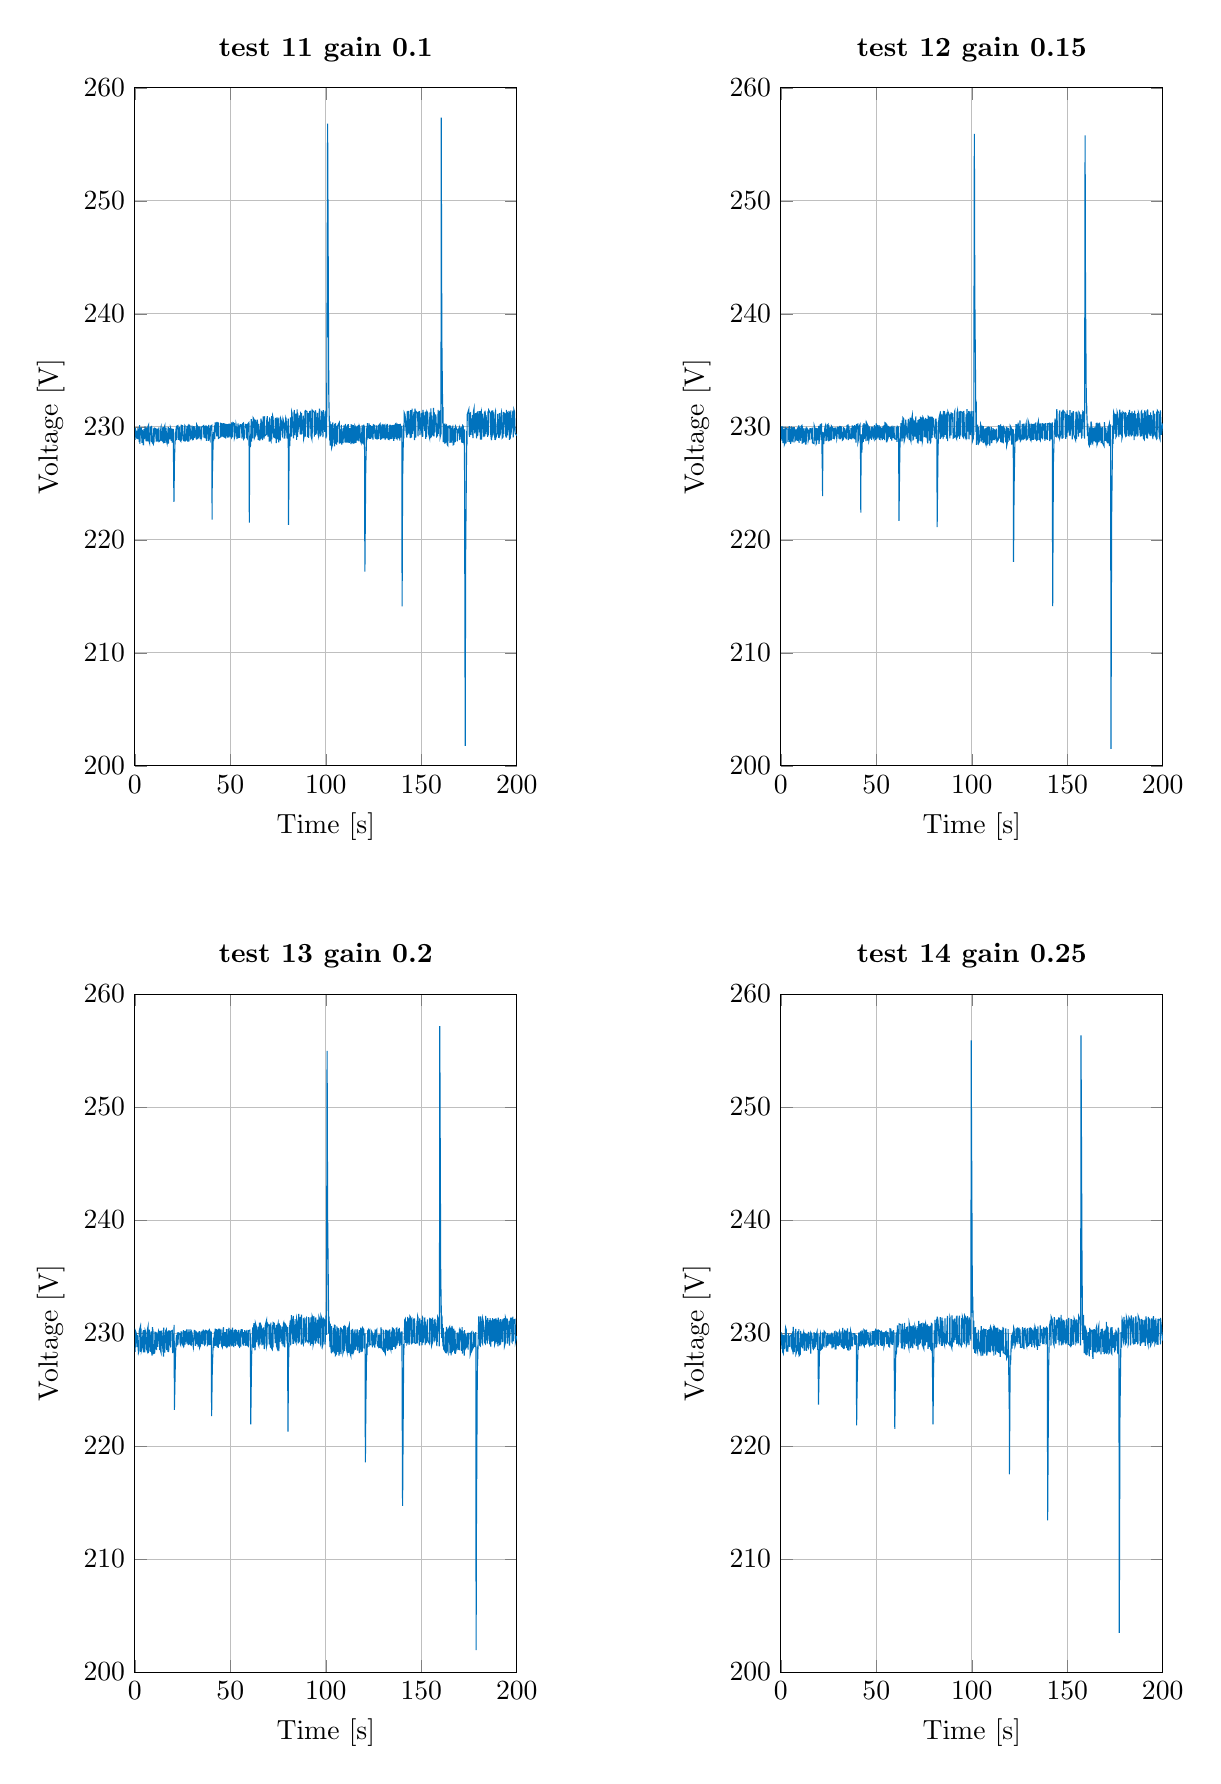
\begin{tikzpicture}

\begin{axis}[%
width=0.4\textwidth,
height=3.39in,
at={(0.953in,6.546in)},
scale only axis,
xmin=0,
xmax=200,
xlabel={Time [s]},
xmajorgrids,
ymin=200,
ymax=260,
ylabel={Voltage [V]},
ymajorgrids,
axis background/.style={fill=white},
title style={font=\bfseries},
title={test 11 gain 0.1}
]
\addplot [color=mycolor1,solid,forget plot]
  table[row sep=crcr]{%
0.016	229.535238881007\\
0.144	228.858129267426\\
0.208	229.908366393416\\
0.976	228.972737272758\\
1.024	229.670033458846\\
1.536	228.917233613161\\
1.584	229.880590212191\\
2.352	228.64358645854\\
2.464	230.15718221907\\
2.608	228.506210212968\\
2.944	229.857712075386\\
3.424	229.890031516869\\
3.728	228.595433629806\\
3.904	229.737789885984\\
4.368	228.431440940234\\
4.528	228.421880735853\\
4.704	229.803954580801\\
5.008	228.915642335785\\
5.296	230.032427980936\\
5.888	228.719473783596\\
5.984	229.896972850776\\
6.608	228.718895766397\\
6.784	229.994080442485\\
7.184	230.168041812437\\
7.296	228.810507827955\\
7.728	228.559110008264\\
8.064	229.94086257001\\
8.544	230.008071593243\\
8.688	228.65109817995\\
8.784	230.087080834804\\
9.168	228.610686746311\\
9.728	228.458908487422\\
9.84	229.855678462227\\
10.048	228.621020351386\\
10.24	229.890620633662\\
10.8	229.849552507557\\
11.184	228.69776920829\\
11.28	229.848053062636\\
11.824	228.723496942051\\
12	229.847172515291\\
12.128	228.701155880547\\
12.592	229.95057559584\\
12.704	228.711165299758\\
13.456	228.835181364439\\
13.6	229.936139511024\\
13.76	230.023649913715\\
13.856	228.847952253558\\
14.528	228.743224163159\\
14.64	229.982742651426\\
15.008	228.542959544791\\
15.2	229.855773470625\\
15.68	230.103685241094\\
15.808	228.582376699034\\
16.336	229.928421071771\\
16.624	228.715315452919\\
16.864	228.544295780524\\
17.456	229.999179979585\\
17.584	228.520854652192\\
18.016	229.876579992395\\
18.384	228.896970724319\\
18.576	229.974705048378\\
18.976	229.774133893815\\
19.04	228.764584873159\\
19.456	229.844923718765\\
19.6	228.60400102699\\
20.096	229.82625521812\\
20.464	223.364765085574\\
20.736	227.067720874282\\
21.2	229.587496697356\\
21.376	228.77364935003\\
21.6	229.948492325871\\
21.856	228.8472025303\\
21.92	230.058342840556\\
22.56	230.119595879508\\
22.784	228.847338925118\\
23.44	229.989799744114\\
23.536	228.844181694744\\
24.096	228.719850414882\\
24.32	230.198300420818\\
24.496	228.791244863064\\
24.96	230.154385308134\\
25.536	228.785349152781\\
26.016	228.766434072724\\
26.16	230.130092496167\\
26.24	230.109743673075\\
26.416	228.766721368489\\
26.896	228.835574778926\\
27.28	230.073168961951\\
27.696	228.70737632534\\
28	230.204642647313\\
28.256	228.688156108701\\
28.4	230.169035587049\\
28.96	230.075928758328\\
29.056	228.929037341186\\
29.696	229.087702374689\\
29.92	230.112241198394\\
30.096	228.811359342027\\
30.24	229.996355471166\\
30.544	228.832022791082\\
30.8	230.062977301986\\
31.216	228.997869429084\\
31.36	230.044504457733\\
32.256	228.874933450876\\
32.4	230.206665999842\\
32.88	230.027738014191\\
33.024	228.919255416821\\
33.2	230.036281742499\\
33.296	229.030753595817\\
33.68	230.039312488709\\
34.256	228.928084496958\\
34.64	230.015431208917\\
34.864	229.016115978586\\
35.024	229.1017544534\\
35.12	229.987783287866\\
36	230.112020749704\\
36.144	229.058169397856\\
36.56	230.085834096126\\
36.704	229.042650979903\\
37.104	229.02552353667\\
37.28	230.134115419709\\
37.456	228.766082050482\\
37.68	230.009674268391\\
38.24	229.96099847578\\
38.416	228.770540112982\\
38.72	230.173946995693\\
39.136	228.966531473144\\
39.376	228.838998034006\\
39.68	230.063319384774\\
40.32	230.141122260726\\
40.448	221.784368702369\\
40.512	225.189701270275\\
41.104	229.543681516169\\
41.232	228.75191271622\\
41.744	230.137754007605\\
41.872	228.921673698896\\
42.064	230.34563027659\\
42.544	230.356982613319\\
42.896	229.159116929914\\
43.024	230.438833406831\\
43.216	229.169632175248\\
43.664	230.392361893368\\
43.776	228.986001577947\\
44.608	229.084434787964\\
44.784	230.355745286841\\
44.976	229.072925879563\\
45.104	230.305607034308\\
45.664	230.251488416548\\
45.776	229.14068661265\\
46.304	230.323372366295\\
46.416	229.145939859769\\
46.896	229.105053245663\\
47.024	230.311459678522\\
47.616	228.97451341693\\
47.744	230.254646497343\\
48.176	229.155943597196\\
48.544	230.236870150585\\
48.656	229.041516739596\\
49.024	230.255564947807\\
49.296	229.081314999036\\
49.344	230.241362991942\\
49.984	230.224961598414\\
50.096	229.202695674357\\
50.496	229.079626555527\\
50.704	230.39444418827\\
51.136	229.071668187226\\
51.424	230.380086788062\\
52.064	230.293818785734\\
52.176	229.041744618653\\
52.416	229.186953611068\\
52.944	230.259285158907\\
53.024	230.178260334608\\
53.456	228.928633528621\\
54.064	230.316367699669\\
54.176	229.077569460977\\
54.256	229.069825010654\\
54.464	230.121000961945\\
54.896	229.034879633446\\
55.104	230.206184161753\\
55.824	230.178451372407\\
56.096	229.04894591641\\
56.176	228.957294960199\\
56.464	230.27218295132\\
56.784	230.328956728434\\
56.976	228.924593476715\\
57.456	229.050454962561\\
57.744	230.226474947225\\
58.464	230.196258779991\\
58.576	229.064372308446\\
58.848	228.976427725103\\
59.104	230.232271094582\\
59.744	230.385996022471\\
59.84	227.040598232009\\
59.952	221.527303204202\\
60.128	229.214747952068\\
60.512	228.205368224979\\
60.944	230.676497152326\\
61.072	228.702789121528\\
61.264	230.491485249688\\
61.712	228.993334895688\\
61.968	230.801295676614\\
62.528	230.625079738033\\
62.656	229.026683897563\\
63.04	229.189564834601\\
63.168	230.628133505251\\
63.984	229.252239089455\\
64.128	230.632602758627\\
64.208	230.452751786673\\
64.576	228.852410440148\\
64.928	230.262117069954\\
65.216	228.832009419298\\
65.616	228.849322729114\\
66.048	230.724910363322\\
66.176	228.950710595869\\
66.288	230.569400780851\\
66.816	228.829464046645\\
67.232	230.927540313875\\
67.68	228.971558520593\\
67.872	230.938333880708\\
67.952	230.6911092455\\
68.064	229.203634887825\\
68.928	229.340262911971\\
68.992	230.499678378771\\
69.392	230.939676483236\\
69.68	229.129568855615\\
70.192	230.470832295193\\
70.4	228.705059707861\\
70.592	230.837754204911\\
71.04	228.840215360789\\
71.36	228.71516713713\\
71.616	230.954861966236\\
71.68	228.893553997604\\
72.176	230.957048153871\\
72.416	230.777542935319\\
72.688	229.110201100843\\
73.28	229.04502465183\\
73.536	230.640822536836\\
73.616	230.802017524795\\
74.064	228.573222541254\\
74.416	230.844763004116\\
74.544	228.891840543072\\
75.056	230.720656300714\\
75.344	228.624321098628\\
75.44	230.817979084364\\
75.504	228.910622357021\\
76.128	228.855692393101\\
76.4	230.706256019752\\
76.8	230.466032347235\\
77.264	229.16495288574\\
77.504	229.102531930812\\
77.6	230.683446095326\\
78.112	230.343265194096\\
78.528	228.972599130904\\
79.04	230.806673699676\\
79.2	230.715073443772\\
79.728	228.970542612795\\
80.304	230.733374657206\\
80.384	226.857059326582\\
80.448	221.327437451402\\
80.864	229.404252371529\\
81.152	228.306958073323\\
81.504	230.843586872558\\
81.936	229.147155562394\\
82.128	231.346200392656\\
82.288	231.246556109186\\
82.816	229.578083192201\\
83.056	228.979768778918\\
83.328	231.220891880682\\
83.552	231.489219984791\\
83.76	229.267300520528\\
84.432	231.177508206234\\
84.72	228.858811896569\\
84.992	231.544402831246\\
85.2	229.125555960708\\
85.376	231.191660584735\\
85.408	229.541276599794\\
86.256	231.012241781408\\
86.624	229.331914832938\\
86.816	231.338206413398\\
87.104	229.30753835664\\
87.28	231.222173845571\\
87.488	229.361881891101\\
88.24	230.992441092442\\
88.448	228.97977360109\\
88.768	229.263897286582\\
89.104	231.431368806669\\
89.248	229.136556425211\\
89.424	231.432517276344\\
90.224	231.342571547677\\
90.352	229.220736006179\\
90.432	229.092512080193\\
90.784	231.221145828582\\
90.992	229.035878876524\\
91.488	231.356001402922\\
92.048	231.386407791167\\
92.176	229.245207967982\\
92.736	228.88958937419\\
92.832	231.391550190008\\
92.896	229.420499562918\\
92.912	231.479840677181\\
93.872	231.28635080499\\
94	229.145891080523\\
94.576	231.469700605431\\
94.64	229.292940493954\\
94.736	231.329358580068\\
94.944	229.366935478867\\
95.696	231.234974865265\\
95.824	229.454497324694\\
96.144	229.204328706469\\
96.56	231.314401740594\\
96.72	231.603241118857\\
97.008	229.203301339133\\
97.568	229.325909459444\\
97.68	231.332929301367\\
98.32	231.184308062864\\
98.448	229.085594355521\\
98.528	229.239352047557\\
98.624	231.48694129223\\
99.408	229.563879740848\\
99.664	231.362168422648\\
100.112	228.975278309684\\
100.224	231.456084201901\\
100.432	229.128987136977\\
100.944	256.84263701152\\
101.568	232.824418066257\\
102.016	228.802206863781\\
102.192	230.477627662055\\
102.304	228.341911852099\\
102.848	230.230766338985\\
103.056	228.155743580583\\
103.456	228.400591862787\\
103.648	230.385289810868\\
104.576	228.272173394227\\
104.688	230.226890187264\\
105.104	230.267643354028\\
105.312	228.553734250331\\
105.632	228.496280503605\\
105.824	230.085310372104\\
106.112	228.628274621467\\
106.224	230.094182210247\\
107.024	230.372192575804\\
107.168	228.510433563278\\
107.264	229.801268545816\\
107.568	228.56740001604\\
108.144	230.181707127603\\
108.32	228.427995960989\\
108.464	229.85805278398\\
109.04	228.556713141071\\
109.056	228.751976362049\\
109.504	230.127378898089\\
110.096	228.603853488475\\
110.224	230.25905219572\\
110.432	228.609900997352\\
110.624	230.105587542716\\
111.248	228.61881939416\\
111.424	230.178967403116\\
111.568	228.608448305603\\
111.744	230.248282971778\\
112.288	228.59549718044\\
112.64	229.89705131924\\
113.168	228.471873966686\\
113.28	230.23438055174\\
113.504	228.582737655951\\
113.696	230.185187079831\\
114.304	228.48665074799\\
114.432	230.147786258873\\
115.056	228.546376751822\\
115.232	230.106841880903\\
115.584	229.962688538295\\
115.776	228.592354166176\\
116.4	230.092982713592\\
116.528	228.851990021563\\
116.576	228.7821827897\\
117.12	230.146514471847\\
117.312	228.71726643071\\
117.52	230.097030997004\\
117.92	229.899160504849\\
118.128	228.781202452306\\
118.528	228.586692154442\\
118.976	229.896955401875\\
119.04	230.156455045858\\
119.248	228.527791697147\\
119.856	230.199383029938\\
120	228.418831902814\\
120.256	230.096665525129\\
120.464	217.192985663592\\
120.912	226.387808906801\\
121.504	230.086996956401\\
121.616	228.869092416391\\
121.824	230.326318027668\\
122.336	229.018081182086\\
122.704	230.309296075824\\
122.896	228.942307687443\\
123.264	230.142920449636\\
123.456	228.933444333022\\
123.824	230.074201586716\\
124.32	228.998427273964\\
124.384	230.093877930818\\
124.736	228.876342666746\\
124.944	230.189444574886\\
125.344	230.151421324278\\
125.84	229.020627358082\\
126.16	228.987636513752\\
126.384	230.088676631487\\
126.704	230.055984033932\\
126.96	228.940383415021\\
127.376	228.965964388971\\
127.584	230.182249021679\\
127.776	228.946462953367\\
127.904	230.161374951553\\
128.464	230.280468621127\\
128.72	228.918631743789\\
129.2	228.968812163731\\
129.344	230.191095476522\\
129.84	228.982292553861\\
129.904	230.273200872645\\
130.32	228.982154880824\\
130.464	230.078180961987\\
130.944	230.179067767849\\
131.04	228.842246446596\\
131.824	230.18060695769\\
131.92	228.986660592228\\
132.144	230.261673177079\\
132.64	228.91041263846\\
133.12	228.877112131825\\
133.184	230.14027736749\\
133.52	228.924478466975\\
133.584	230.201477552179\\
134	228.919188437134\\
134.224	230.150777340184\\
134.72	228.946078464361\\
135.024	230.163232651447\\
135.6	228.763046776212\\
135.744	230.184900283927\\
136.016	228.938623804962\\
136.304	230.210614437406\\
136.624	230.276056738916\\
136.8	229.022900115861\\
137.28	228.933212383056\\
137.424	230.287851470524\\
137.92	228.985175825772\\
138.224	230.247332557497\\
138.8	228.789213748309\\
138.944	230.112563368255\\
139.024	230.273971912359\\
139.12	229.079785744628\\
139.824	230.10780050095\\
139.952	214.12174360206\\
140.208	225.369332070032\\
140.752	230.158997989308\\
140.864	228.989080283176\\
141.056	231.257267241533\\
141.536	231.046869075331\\
142	229.663721049397\\
142.464	229.043502997064\\
142.576	231.362814875453\\
142.864	229.29244343937\\
142.96	231.42358766716\\
143.328	229.403266705954\\
143.44	231.421819495863\\
144.208	229.015504561871\\
144.48	231.490542449426\\
144.848	229.041436959466\\
145.184	231.603327011738\\
145.392	229.37455796258\\
146.144	231.315912529346\\
146.432	228.827437542576\\
146.704	231.618315506495\\
147.072	229.054587166289\\
147.248	231.357621948425\\
148.128	231.190940829464\\
148.256	229.335264456056\\
148.336	229.154533225651\\
148.528	231.309484781206\\
149.072	231.340443239522\\
149.28	229.278227777841\\
150.032	231.234449383143\\
150.16	229.586311947894\\
150.56	229.12442505588\\
150.672	231.253950380168\\
150.8	229.13256673022\\
150.896	231.510134391869\\
151.792	229.639647342278\\
152.016	231.335178143239\\
152.304	228.934547979746\\
152.576	231.38072100783\\
152.704	229.111731095027\\
152.96	231.358137651363\\
153.36	231.226411744671\\
153.744	229.463217016105\\
154.368	229.012854343614\\
154.48	231.278555348861\\
154.928	229.005131398957\\
155.024	231.644102940393\\
155.312	229.110709875913\\
155.424	231.018518503606\\
156.192	229.186160118325\\
156.384	231.6697344582\\
156.672	229.16100648332\\
156.848	231.282112178535\\
157.056	229.497479111405\\
157.088	231.065377311703\\
157.648	231.042946319707\\
158.096	229.153113728608\\
158.496	229.234757817769\\
158.832	231.498715277065\\
158.96	229.38872194146\\
159.072	231.256936099707\\
159.632	231.358269847518\\
159.84	229.064953143242\\
160.32	229.413161448843\\
160.432	257.362637006676\\
160.752	238.034917805452\\
161.248	230.307309715383\\
161.376	231.753194925804\\
161.52	228.641811453001\\
162.176	230.290738879039\\
162.32	228.567239250711\\
162.784	228.617515242154\\
162.976	230.204790937423\\
163.296	230.154876621706\\
163.52	228.465137119373\\
163.92	228.353429490609\\
164.112	230.051321367515\\
164.912	230.08957733177\\
165.056	228.57500465852\\
165.312	230.077738146695\\
165.536	228.683963907295\\
165.888	228.657466152347\\
166.032	229.858757373718\\
166.464	230.01762270179\\
166.688	228.409096365446\\
167.088	228.450258333231\\
167.312	229.904423032042\\
167.808	228.643963780631\\
167.952	230.045848173927\\
168.752	229.738930441405\\
168.864	228.729451021024\\
169.312	229.70165083931\\
169.984	229.975952398584\\
170.096	228.828857632574\\
170.688	229.955069851683\\
171.216	228.619757728242\\
171.328	230.027153886637\\
171.632	228.584877296102\\
171.728	230.117500176993\\
171.968	230.067460018643\\
172.432	228.391029363415\\
172.608	229.770531283648\\
173.008	201.760336451302\\
173.216	218.368058119048\\
173.808	229.640390084592\\
173.904	228.335612013469\\
174.08	231.102685228418\\
174.88	231.541508214931\\
175.088	229.342239802585\\
175.328	229.126854018568\\
175.44	231.180284151087\\
175.824	231.239935325399\\
176.032	229.304046126396\\
176.864	231.045780984407\\
176.912	229.435755164557\\
177.072	228.998420382776\\
177.264	231.333911437507\\
177.648	231.647416663512\\
177.936	229.42761798724\\
178.528	231.215398307918\\
178.816	229.376566440522\\
178.976	228.989372672063\\
179.168	231.292977778456\\
179.536	229.184103424102\\
179.712	231.391613230605\\
180.496	229.518048704454\\
180.592	231.39234521676\\
180.96	228.864959319565\\
181.232	231.231349688624\\
181.392	231.354539312256\\
181.6	228.881555533359\\
182.016	231.179006711812\\
182.56	229.610440053854\\
182.784	229.090756352027\\
183.056	231.340383464857\\
183.264	229.15546018168\\
183.44	231.440656183043\\
183.808	229.358267933257\\
183.92	231.046893176433\\
184.768	229.115928830554\\
184.96	231.360735051225\\
185.088	229.246504659334\\
185.264	231.503104269667\\
186.144	231.228668216879\\
186.208	229.557503940032\\
186.752	228.819603963219\\
186.864	231.435534600365\\
187.072	229.074104776732\\
187.408	231.466635836218\\
187.616	229.254007311664\\
187.728	231.274909236258\\
188.576	228.842627807319\\
188.768	231.347230126033\\
188.848	231.396730941929\\
189.136	229.075063974813\\
189.856	229.440040110105\\
190.032	231.158919111455\\
190.56	229.026754169886\\
190.976	231.21883365964\\
191.12	229.239931675971\\
191.344	229.352135218573\\
191.856	231.204795067808\\
191.936	231.266468391811\\
192.384	229.016979522078\\
192.864	229.125206489148\\
192.88	231.327296674006\\
193.168	229.388716317455\\
193.44	231.212803650354\\
193.92	231.144671752121\\
194.288	229.067084779855\\
194.56	231.511531911796\\
194.688	229.050782074503\\
195.024	231.340891649923\\
195.152	229.243796969616\\
195.904	231.412303425797\\
196.192	228.852414259453\\
196.384	231.336423749912\\
196.592	228.960968211002\\
196.928	231.459806956877\\
196.992	229.308484709138\\
197.968	231.431946289716\\
198.096	229.344086201103\\
198.176	229.082975943049\\
198.528	231.506359860785\\
198.832	231.326499352754\\
199.12	229.449692162571\\
200	229.232533531238\\
};
\end{axis}

\begin{axis}[%
width=0.4\textwidth,
height=3.39in,
at={(4.183in,6.546in)},
scale only axis,
xmin=0,
xmax=200,
xlabel={Time [s]},
xmajorgrids,
ymin=200,
ymax=260,
ylabel={Voltage [V]},
ymajorgrids,
axis background/.style={fill=white},
title style={font=\bfseries},
title={test 12  gain 0.15}
]
\addplot [color=mycolor1,solid,forget plot]
  table[row sep=crcr]{%
0.016	228.938541964618\\
0.192	230.034655794883\\
0.576	228.781388084923\\
0.992	230.036113863287\\
1.136	228.557543008092\\
1.568	229.797797238747\\
1.856	228.436860560971\\
2.096	228.557193050054\\
2.208	230.025470002028\\
2.672	228.542426449571\\
2.768	229.845459344511\\
3.648	229.80609670027\\
3.744	228.672543243947\\
3.776	228.703948962233\\
4.368	230.067700419714\\
4.656	228.661669776231\\
5.008	229.852457564791\\
5.136	228.495142571539\\
5.504	230.044254939326\\
5.696	228.686980453717\\
5.824	229.936465837068\\
6.432	228.625809641321\\
6.544	229.94034480947\\
7.104	229.924998150714\\
7.408	228.764351808432\\
7.648	228.850760967019\\
7.824	229.766946354634\\
8.528	228.762262387965\\
8.624	229.964076314137\\
8.8	228.774085190709\\
9.344	230.123260536946\\
9.536	228.590695725754\\
9.664	229.997970571277\\
10.368	228.775263259059\\
10.464	230.019309770227\\
11.024	230.130061146406\\
11.168	228.50477630886\\
11.264	230.076144178636\\
11.648	228.636934525256\\
11.968	228.657107010784\\
12.08	229.874000533759\\
12.944	228.424638336973\\
13.072	229.942118548927\\
13.184	228.444822790134\\
13.632	229.888430920136\\
14.192	229.726011654402\\
14.336	228.808073040029\\
14.576	228.998299224388\\
14.96	229.742828287583\\
15.168	228.838854802719\\
15.28	229.844897127746\\
16	229.819722084294\\
16.208	228.900651709746\\
16.416	229.932670539384\\
16.544	228.589054132567\\
17.344	228.526241232012\\
17.456	230.119636438483\\
17.856	229.876415453881\\
18.08	228.79122661717\\
18.256	229.905392249551\\
18.48	228.483236000718\\
18.72	228.568575117726\\
19.008	229.884228435761\\
19.6	228.832513236347\\
19.856	230.08900694483\\
20	228.490795698046\\
20.576	230.180667881191\\
20.976	230.191079752055\\
21.088	228.839316307794\\
21.296	230.301070831415\\
21.824	225.162206696233\\
21.84	223.862833153024\\
22.016	229.545966312358\\
22.464	228.477279190253\\
23.056	229.97537342566\\
23.376	230.13200192733\\
23.6	228.801455065418\\
24	228.824607800195\\
24.256	230.136053837118\\
24.736	230.230751699879\\
24.88	228.734291937985\\
25.056	230.143779111124\\
25.28	228.791958892913\\
25.6	228.835451103995\\
25.776	229.963808080512\\
26.4	228.803937486844\\
26.528	230.069146666808\\
27.168	229.900053987547\\
27.28	228.941793105038\\
27.488	229.897381073911\\
28	228.897869046269\\
28.096	229.922122354178\\
28.24	229.051438805904\\
28.848	229.942868307241\\
29.28	228.971664428815\\
29.36	229.069095510704\\
29.776	229.970405062584\\
30.256	229.957323889733\\
30.4	228.953491738031\\
30.816	230.095030484474\\
30.992	228.886374670905\\
31.168	230.060460012896\\
31.28	228.943658719657\\
31.808	230.034635852725\\
32.24	228.825071768107\\
32.72	228.917416520128\\
32.896	229.978296723622\\
33.04	229.095225444627\\
33.248	229.887076600367\\
33.68	228.97889710579\\
34.256	229.862610706802\\
34.32	228.89163810289\\
34.656	230.110609895094\\
35.136	230.1657286943\\
35.312	228.836286647525\\
35.616	230.087130661053\\
36.112	228.971797478693\\
36.592	228.988543758273\\
36.736	229.907103602764\\
37.008	228.901144553378\\
37.376	230.128723959783\\
37.488	228.989868220858\\
38.016	230.067458132705\\
38.368	228.913792269113\\
38.496	230.157579342515\\
39.088	228.88269402946\\
39.216	230.113616198342\\
39.344	228.613372847309\\
39.536	230.187898069725\\
40.256	230.250467770627\\
40.384	228.665302078408\\
40.624	228.866903940063\\
41.056	230.069168856409\\
41.456	230.203790791366\\
41.76	226.878049952568\\
41.872	222.420758046394\\
42.016	229.324754313279\\
42.4	227.713877708019\\
42.976	230.187148041988\\
43.2	228.681339719754\\
43.536	230.320078384646\\
43.68	228.920396579647\\
44.096	230.209561886556\\
44.56	228.748848098607\\
44.736	230.42358063291\\
45.296	230.207071982596\\
45.44	228.778791881322\\
45.616	230.167047346538\\
46.08	228.782923210271\\
46.16	228.854877805602\\
46.256	230.04071248684\\
46.96	228.964644273351\\
47.376	230.0209655175\\
47.52	228.854857815804\\
48.096	230.008580123947\\
48.432	229.074442320175\\
48.8	228.926494618283\\
48.976	230.143605876566\\
49.712	228.822629338994\\
49.856	230.064124531875\\
49.936	230.30554495019\\
50.24	228.933169432014\\
50.496	230.184834341024\\
50.688	229.043349652658\\
51.376	230.145895102617\\
51.552	228.925976011372\\
51.92	228.886969182476\\
52.096	230.026588065765\\
52.768	228.981075696275\\
52.816	229.941749395979\\
53.072	228.824276606301\\
53.536	230.078645518102\\
53.792	228.930300141759\\
54.096	230.159232960406\\
54.32	228.836448041328\\
54.496	230.375491158536\\
55.136	230.302517434702\\
55.312	228.627170148835\\
55.536	230.237521377886\\
55.84	228.863370293741\\
56.208	229.037546606369\\
56.336	230.081923922438\\
56.72	229.117930155469\\
57.136	230.00684069916\\
57.472	228.940109199201\\
57.856	230.049360307486\\
58.048	228.78487587817\\
58.256	230.107766049843\\
58.688	229.015627042545\\
59.216	230.082816380154\\
59.472	228.953412578075\\
60.272	228.901787615759\\
60.416	229.967874009152\\
60.8	228.670592598728\\
60.976	230.1109058459\\
61.152	229.000982067589\\
61.616	230.040433455539\\
61.696	229.830412816039\\
61.84	221.687461498395\\
62.32	227.999823482332\\
62.896	230.322847412468\\
63.424	228.708350904728\\
63.536	230.582456739274\\
63.824	228.989943672156\\
63.936	230.812989947006\\
64.4	230.696614719419\\
64.624	228.752140776427\\
65.088	229.081272000532\\
65.36	230.645837092501\\
65.44	230.530830230703\\
66.016	229.180783023429\\
66.176	229.119204980892\\
66.64	230.396736393021\\
66.8	230.697330855885\\
67.168	228.820785556188\\
67.76	230.808379070564\\
67.888	228.869779041391\\
68.128	228.709637614437\\
68.544	230.749858296577\\
68.864	231.030939865804\\
69.152	228.78806794665\\
69.264	230.723226654617\\
69.472	228.884591527328\\
69.984	230.562598373015\\
70.176	229.137487708366\\
70.704	230.935192707477\\
70.848	228.934724884273\\
71.104	230.381195501662\\
71.552	228.614146303546\\
71.744	230.598511549314\\
71.872	228.520033728644\\
72.384	230.679714667206\\
72.912	228.739921369481\\
73.088	230.895329898238\\
73.472	228.719235066768\\
73.728	230.832719115091\\
74.096	228.679994709275\\
74.256	228.829295289017\\
74.448	230.84213113261\\
74.928	230.651387923606\\
75.232	229.099266810719\\
75.808	230.790771892548\\
76.032	229.053056721185\\
76.368	230.712500087311\\
76.656	228.990108642532\\
76.896	228.550948200957\\
77.168	230.925562074171\\
77.568	230.837102943062\\
77.856	228.791216774368\\
78.192	230.909447689884\\
78.336	228.613353207951\\
78.576	228.67984457639\\
78.752	230.90282848808\\
79.2	229.023134135095\\
79.552	230.782106482864\\
79.872	230.704882936923\\
80.384	229.185682828315\\
80.736	229.083054199766\\
80.992	230.682178478203\\
81.312	230.676414037437\\
81.616	228.939696171616\\
81.712	230.432589591844\\
81.84	221.12646619725\\
82.288	227.820931446095\\
82.736	230.725444218918\\
83.216	231.057166375222\\
83.424	228.947474193357\\
83.536	231.370770918249\\
83.824	229.072683836835\\
84.208	229.185268435007\\
84.32	231.153370140871\\
85.008	228.908671209741\\
85.12	231.420828161362\\
85.488	229.11305379768\\
85.664	231.391708161694\\
86.032	229.288613724172\\
86.544	231.177296638441\\
86.752	228.971083341178\\
87.104	231.298820635285\\
87.312	228.740455760544\\
87.488	231.353125488602\\
88.288	231.003884616242\\
88.496	228.979439407442\\
88.928	231.157929629047\\
89.136	229.247635769938\\
89.232	231.225171059474\\
89.952	231.154555550519\\
90.24	229.004821140702\\
90.8	229.074276829315\\
90.976	231.361334015374\\
91.056	231.399038898399\\
91.184	229.308726903146\\
92.064	228.940586906448\\
92.176	231.203466090198\\
92.48	231.436203358232\\
92.544	229.136212183175\\
93.216	229.300020227654\\
93.36	231.348384931151\\
93.648	228.937601172948\\
93.76	231.382044963248\\
94.128	229.253068250186\\
94.224	231.344902799862\\
95.024	231.292659706269\\
95.152	229.186651484039\\
95.632	229.061943745118\\
95.808	231.418790495913\\
95.968	230.975582690697\\
96.096	229.388450912664\\
96.816	229.036388155587\\
97.008	231.103904316107\\
97.376	228.910697386581\\
97.472	231.560223996186\\
98.096	229.584730228672\\
98.352	231.395238480009\\
98.56	228.902121335737\\
98.832	231.312118881447\\
99.136	231.323090213837\\
99.344	229.282351215748\\
100.016	231.420409561063\\
100.304	228.720148545334\\
100.784	228.979057547894\\
100.88	231.403272993676\\
101.024	229.25985169385\\
101.328	255.933495679891\\
101.568	241.880064968773\\
102.176	229.56393233827\\
102.304	232.238902022956\\
102.432	228.418417171983\\
103.024	230.19640296265\\
103.408	228.439998284027\\
103.504	229.989969802642\\
103.648	228.564788540418\\
104.128	228.750242247105\\
104.624	230.212027962756\\
104.864	230.034091803579\\
105.008	228.686404354178\\
105.344	230.107260812124\\
105.888	228.605895386233\\
105.984	230.061867948036\\
106.128	228.573930848041\\
106.864	229.87094635134\\
106.928	228.682320407079\\
107.408	228.41722361703\\
107.52	229.901344994113\\
107.968	228.367184615695\\
108.08	229.991082105765\\
108.448	228.468030988871\\
108.64	229.990832126454\\
109.2	229.95394814709\\
109.408	228.338101384335\\
110.16	229.991675572206\\
110.288	228.842379265671\\
110.352	229.694841515622\\
110.464	228.574450100461\\
111.072	229.88133981427\\
111.184	228.82611178255\\
111.712	229.806415403172\\
111.824	228.831455825566\\
112.192	229.758580337375\\
112.768	228.795192128347\\
112.88	229.843263763718\\
113.136	228.673703700781\\
113.856	228.856931105007\\
114	230.16023042473\\
114.464	228.965733190984\\
114.56	230.048586501724\\
115.04	230.144397987895\\
115.168	228.655792484705\\
115.68	230.074583209057\\
115.808	228.606692831716\\
116.4	230.038819247792\\
116.528	228.536661775768\\
116.64	229.9972788521\\
117.216	229.815141924334\\
117.744	228.63205603462\\
118.176	230.010381544019\\
118.304	228.349181266537\\
118.544	228.545444079074\\
118.896	229.929688923207\\
119.024	228.675438681354\\
119.136	229.88154793151\\
119.92	228.79238506193\\
120.096	230.09479326536\\
120.768	229.860687342225\\
120.88	228.427171726161\\
121.296	229.765394009202\\
121.696	229.730945668718\\
121.856	218.054111159093\\
122.128	224.539957425427\\
122.64	229.40935121403\\
122.816	228.641288807692\\
123.12	230.236216449234\\
123.376	228.722557388479\\
123.6	230.215140953345\\
124.016	228.785749783893\\
124.24	230.371234634185\\
124.976	228.864714803331\\
125.2	230.574724888503\\
125.28	230.298302699736\\
125.456	228.756889733085\\
126.096	228.962742805415\\
126.4	230.230750138479\\
126.816	228.833873908569\\
126.96	230.283278520104\\
127.136	228.896312893085\\
127.36	230.287633078398\\
127.776	228.923836355376\\
128.32	230.216818875478\\
128.48	230.331676872138\\
128.656	228.863119503417\\
129.376	228.962960283738\\
129.52	230.53099338452\\
129.84	230.357596827067\\
130.144	229.03536457893\\
130.4	230.257642335874\\
130.576	228.907432770377\\
130.976	228.779696639632\\
131.28	230.276304280893\\
131.616	228.844876987503\\
132	230.237003327848\\
132.256	228.854498223202\\
132.64	230.237935912279\\
133.04	230.250100688307\\
133.216	228.87329534697\\
133.52	230.395689244799\\
133.936	228.810348781013\\
134.256	228.849080991154\\
134.56	230.315032574537\\
134.88	230.528049244666\\
135.216	228.85210517813\\
135.6	230.280568826074\\
135.776	228.835411480498\\
135.856	228.809075474865\\
135.92	230.311010705506\\
136.576	228.989923442271\\
136.88	230.333317854089\\
137.104	228.903307995112\\
137.36	230.247641056232\\
138	230.17479018262\\
138.256	228.766693242216\\
138.48	230.326051153659\\
138.656	228.945027030298\\
139.264	228.969107600441\\
139.44	230.32053111539\\
139.616	228.861011343506\\
139.84	230.257625530806\\
140.64	230.316898041378\\
140.816	228.802606317109\\
140.864	228.740550207842\\
141.04	230.298465937593\\
141.44	230.24353953691\\
141.536	228.896393467122\\
142.16	230.399669796222\\
142.352	214.126414657809\\
142.72	226.7223069635\\
143.248	229.952786493513\\
143.648	230.737911822267\\
143.936	229.166387285576\\
144.416	229.119614432733\\
144.512	231.560069481253\\
144.672	231.196034189766\\
144.8	229.35740605712\\
145.68	229.042713711739\\
145.792	231.104415747214\\
146.096	231.448733278893\\
146.16	229.102826760494\\
146.864	229.620183127979\\
147.056	231.357914909945\\
147.264	228.948986961737\\
147.536	231.46619431373\\
147.744	229.013933247874\\
147.92	231.43568748026\\
148.8	231.24743808048\\
148.928	229.36250177321\\
149.168	228.93912890084\\
149.36	231.157634818617\\
149.808	229.090649218495\\
149.904	231.460816099063\\
150.192	229.483059260204\\
150.784	231.03496176268\\
151.152	229.223371341163\\
151.408	231.473098154075\\
151.472	229.215385061457\\
152.368	231.252289537585\\
152.576	228.892183165115\\
152.656	229.088909573127\\
153.152	231.398127912902\\
153.312	231.182376535168\\
153.44	229.278883816712\\
154.32	228.845066713942\\
154.512	231.315982321356\\
154.88	228.913927995755\\
154.976	231.337945716375\\
155.216	231.052843048636\\
155.744	229.432222772961\\
155.904	229.137634151402\\
156.096	231.312200279185\\
156.48	231.220170855161\\
156.608	229.480861130202\\
157.2	231.10460735411\\
157.488	229.034853052534\\
157.648	229.055915749212\\
158.144	231.383640667249\\
158.624	231.304911179166\\
158.832	229.314093878502\\
159.072	228.95629344626\\
159.328	255.799518274073\\
159.536	242.009227802376\\
160	231.177655555163\\
160.128	232.121315762248\\
160.56	229.187324749166\\
160.752	230.288276385437\\
161.216	228.457713266219\\
161.536	228.336856480896\\
161.728	229.945595932176\\
162.336	228.394147721389\\
162.448	230.471008736754\\
162.768	230.099739617856\\
162.992	228.679731155211\\
163.312	228.547036487278\\
163.488	229.937303369433\\
164.112	228.716317424986\\
164.288	229.952828184467\\
164.912	228.640189690095\\
165.088	230.288805301807\\
165.44	230.318731422648\\
165.584	228.421101473989\\
165.984	228.650621263606\\
166.128	230.299839799843\\
166.64	228.657374251629\\
166.848	230.365074586135\\
167.248	229.931978505765\\
167.376	228.782341465356\\
167.648	229.941695633917\\
167.792	228.563297332929\\
168.288	229.994170593858\\
168.432	228.599849988572\\
169.248	228.305612957611\\
169.424	230.411864849636\\
169.76	229.782377673637\\
169.968	228.761825632322\\
170.176	229.897880927508\\
170.72	228.696380800295\\
171.12	228.615841091032\\
171.264	230.048081372731\\
171.44	228.564559628119\\
171.664	230.025984926142\\
171.984	230.245937650236\\
172.112	228.298134134341\\
172.704	230.221748209866\\
172.896	201.504101070558\\
173.216	221.904765967813\\
173.792	230.102525764546\\
174	228.487528339788\\
174.256	231.311871955368\\
174.496	231.172323718467\\
174.992	229.376981245252\\
175.216	231.154002200449\\
175.504	229.112779125152\\
175.904	229.266660791017\\
176.08	231.340043650889\\
176.4	231.143716164873\\
176.928	229.523425131013\\
177.008	229.104000163591\\
177.504	231.524481658175\\
177.712	229.309780859578\\
177.904	231.183430700017\\
178.224	231.232319944257\\
178.592	228.958316597157\\
178.832	229.13213659299\\
179.088	231.325897515501\\
179.968	231.162542808869\\
180.032	229.488049586567\\
180.336	229.308997046539\\
180.448	231.239040965983\\
180.752	231.19935014018\\
180.896	229.137841510329\\
181.632	231.069722547726\\
181.92	229.195399296149\\
182.192	231.286742306861\\
182.4	229.137420921785\\
182.576	231.507874587689\\
182.704	229.318953049481\\
183.216	231.205853718945\\
183.504	229.165836270677\\
183.92	231.371104245036\\
183.984	229.249459729629\\
184.72	231.220832256284\\
185.008	228.836157684755\\
185.28	231.428890790115\\
185.568	229.155593090725\\
185.712	229.413743985409\\
185.824	231.123211071385\\
186.592	229.136647721284\\
186.864	231.219922646385\\
187.072	229.235499923623\\
187.248	231.274569182828\\
187.568	231.111673155962\\
188.032	229.544430756093\\
188.336	229.141906578726\\
188.752	231.337137767472\\
188.912	231.386632113621\\
189.04	229.183358953876\\
189.712	231.241888250294\\
189.92	228.984774969539\\
190.4	228.864905988485\\
190.576	231.458508333916\\
190.704	229.309572586967\\
190.816	231.320105341104\\
191.584	229.006899404996\\
191.776	231.453133625815\\
191.984	228.971398630156\\
192.08	231.556058559124\\
192.864	229.368035663748\\
193.04	231.039616448819\\
193.248	229.226417684397\\
193.664	231.277507960136\\
193.808	229.182548706723\\
194.064	231.033735355564\\
194.832	228.922304105146\\
195.024	231.440322550729\\
195.152	229.162065294254\\
195.728	231.174767109803\\
195.856	229.372591961993\\
196.576	229.032530246337\\
196.768	231.349726556016\\
197.056	228.905639248373\\
197.152	231.462500221675\\
197.952	231.25713063094\\
198.08	229.175319744526\\
198.56	228.918507737537\\
198.736	231.45622277651\\
198.816	231.220687795079\\
199.36	229.30388454795\\
200	230.29743227934\\
};
\end{axis}

\begin{axis}[%
width=0.4\textwidth,
height=3.39in,
at={(0.953in,2.015in)},
scale only axis,
xmin=0,
xmax=200,
xlabel={Time [s]},
xmajorgrids,
ymin=200,
ymax=260,
ylabel={Voltage [V]},
ymajorgrids,
axis background/.style={fill=white},
title style={font=\bfseries},
title={test 13  gain 0.2}
]
\addplot [color=mycolor1,solid,forget plot]
  table[row sep=crcr]{%
0.016	229.790193437374\\
0.144	228.334693372898\\
0.288	230.196008864829\\
0.688	230.028557530489\\
1.136	228.74912723183\\
1.328	229.832333863015\\
1.872	228.248854438156\\
2.192	228.433580072759\\
2.304	230.197878998509\\
2.944	230.606188403232\\
3.088	228.34560991134\\
3.264	230.384348239379\\
3.408	228.460994805229\\
3.76	228.732483082772\\
4.336	230.223571351565\\
4.48	228.286620283023\\
4.624	230.264550790354\\
5.2	228.292152373918\\
5.344	230.263361544791\\
5.664	230.114915699669\\
6.112	228.595404684424\\
6.496	228.417019414525\\
6.624	230.34556444848\\
6.944	230.601069197173\\
7.072	228.218641708625\\
7.584	230.313648789489\\
8.048	228.349676478322\\
8.56	230.150810651711\\
8.704	228.431797827844\\
9.024	228.002908213296\\
9.2	230.519215895497\\
9.52	230.122682024679\\
9.664	228.182699562683\\
10.384	228.23037841899\\
10.48	230.071243600317\\
10.88	230.066931520466\\
11.024	228.608506701391\\
11.344	228.569690612426\\
11.52	230.054106252006\\
12.016	228.779838102015\\
12.4	230.195487786701\\
12.88	229.976185837783\\
12.992	228.492373440335\\
13.12	230.195949922256\\
13.504	228.410431694959\\
13.744	228.268327110071\\
13.84	230.207574686713\\
14.784	228.315326865739\\
14.88	230.259032146712\\
15.024	227.919152586845\\
15.136	230.476003845583\\
15.664	228.270923152079\\
16.176	230.21930123355\\
16.496	230.327641497825\\
16.72	228.486992933299\\
16.848	230.145370196671\\
17.36	228.332254808068\\
17.536	230.230955141992\\
17.68	228.325370341797\\
18.208	230.24553692762\\
18.704	228.81313197196\\
18.72	228.816142183807\\
18.848	230.151876895401\\
19.616	230.228223393736\\
19.76	228.230523791285\\
20.08	228.636835558574\\
20.576	230.716555676845\\
20.704	223.198095809652\\
21.28	228.135827067673\\
21.776	229.836261183777\\
21.872	228.803279428393\\
22.336	230.069989283615\\
22.512	228.926597738856\\
22.896	230.012751613309\\
23.536	229.968192526458\\
23.68	229.076494324576\\
23.968	228.952832409069\\
24.256	230.104808833219\\
24.576	230.086964935717\\
24.768	229.06894267129\\
25.344	228.86583347603\\
25.456	230.262483392765\\
25.664	228.768941469347\\
26.096	230.164685173702\\
26.304	228.978311902693\\
26.576	230.098330101147\\
26.976	230.210369427371\\
27.248	229.060779883738\\
27.856	230.328382012648\\
27.984	228.934530088224\\
28.176	230.108065331577\\
28.608	229.003337757811\\
28.816	230.327936198901\\
29.104	228.989482493703\\
29.504	228.93291150807\\
29.616	230.155389184031\\
29.936	230.039879802947\\
30.544	228.826783059765\\
30.624	228.745793786495\\
31.136	230.228962240405\\
31.536	230.193689758032\\
31.744	228.868950778606\\
32.176	230.1566506139\\
32.368	229.055304512289\\
32.656	230.040114140352\\
32.768	228.975202602103\\
33.056	230.064301886959\\
33.104	228.754882808914\\
33.696	230.160820592223\\
33.904	228.698006447887\\
34.384	228.911283912952\\
34.576	230.135483491258\\
35.088	229.045642592373\\
35.216	230.206355224201\\
35.728	228.985164649606\\
35.936	230.231859253056\\
36.496	230.131961906386\\
36.608	228.967534934914\\
36.928	229.036056753417\\
37.056	230.237595678369\\
37.776	230.181102634192\\
37.968	228.915436369006\\
38.448	229.034951295248\\
38.576	230.199082069543\\
38.976	230.283040543294\\
39.088	228.940196083118\\
39.296	230.244260437713\\
39.808	228.966902703295\\
40.016	230.136359913018\\
40.192	222.648176349269\\
40.544	226.849088771048\\
41.136	229.591196803545\\
41.312	228.686293487702\\
41.696	230.116283344604\\
41.952	228.872984631131\\
42.096	230.401715488034\\
42.64	228.898063247944\\
42.896	230.352394029613\\
43.12	228.769861337778\\
43.296	230.285822778267\\
43.68	228.684795744518\\
43.856	230.351827599126\\
44.256	230.350022029947\\
44.4	229.010386110512\\
45.056	230.36694281027\\
45.44	228.876537144553\\
45.76	228.747224721658\\
46.096	230.188022752848\\
46.416	230.512892340339\\
46.56	228.855086831751\\
47.056	230.089356006955\\
47.28	228.904365792668\\
47.6	228.843042669735\\
47.936	230.297372687759\\
48.256	230.298188199444\\
48.4	228.798107974323\\
48.8	228.929312944532\\
49.216	230.418861990597\\
49.296	230.416255975506\\
49.44	228.807104110164\\
50.176	230.332407353159\\
50.4	228.826224147973\\
50.576	230.274848609033\\
50.96	228.887615840231\\
51.136	230.480306397812\\
51.52	228.878200639649\\
51.76	228.832175468891\\
52.016	230.207938495726\\
52.448	230.263323942589\\
52.64	228.861748284896\\
53.136	230.271660831632\\
53.6	229.091599531883\\
53.68	228.97650334669\\
54.096	230.241439114891\\
54.24	228.829185287186\\
54.416	230.281892790554\\
54.864	228.681797732342\\
55.376	230.174185700622\\
55.472	228.794366368355\\
55.616	230.297997218446\\
56.256	230.286880364489\\
56.512	229.001419866711\\
56.736	230.082802224659\\
56.88	228.893958526048\\
57.536	230.252756280407\\
57.904	228.901066711854\\
58.016	230.158199850784\\
58.16	228.869730878905\\
58.656	230.278040312577\\
58.88	228.942532572869\\
59.36	228.842790748833\\
59.456	230.208703651852\\
60.176	230.259865360821\\
60.4	228.892103305257\\
60.496	229.95070019234\\
60.688	221.911526610546\\
61.104	227.769352154973\\
61.696	230.49406071159\\
62.064	228.699090124781\\
62.256	230.648686886928\\
62.416	230.867082975747\\
62.864	228.478183993307\\
63.024	228.784900892082\\
63.12	230.878222240564\\
63.6	230.573343953275\\
63.648	229.173398654558\\
64.56	230.571489346586\\
64.624	229.032325445592\\
64.928	228.883757768969\\
65.28	230.926304409999\\
65.488	228.973443210825\\
65.984	230.715496286007\\
66.304	230.560907340122\\
66.512	228.911551333846\\
66.704	230.404449954464\\
67.12	228.973782762035\\
67.424	230.505831678998\\
67.792	228.580807645309\\
68.112	228.954675373537\\
68.304	230.700263226937\\
68.928	231.107975593185\\
68.992	228.833595911317\\
69.216	229.015986595437\\
69.328	230.902093252397\\
70.208	230.618556070578\\
70.304	229.010648656017\\
70.528	230.768078617746\\
70.976	228.713191870422\\
71.248	230.918032686609\\
71.376	228.719493771491\\
71.936	228.552572826044\\
72.192	230.703340854071\\
72.336	228.738737832128\\
72.432	230.932720092779\\
72.992	230.860525988687\\
73.536	229.115090288858\\
74.032	230.724683223294\\
74.16	228.878603708662\\
74.56	228.662169330863\\
74.752	230.66849984198\\
74.992	230.837343864501\\
75.12	228.75439634358\\
75.44	228.398995853355\\
75.616	230.862847064207\\
76.064	229.212460726062\\
76.176	230.677239581332\\
77.12	229.018515531604\\
77.216	230.576842576206\\
77.664	228.820569902509\\
77.856	230.870549584719\\
77.936	230.910493498447\\
78.464	228.953036170692\\
78.544	228.726277499533\\
78.72	230.795172936267\\
79.28	230.613028097783\\
79.776	229.064329438748\\
79.92	230.545931076243\\
80.208	221.278530317745\\
80.416	226.889236487023\\
80.944	230.422747056434\\
81.424	231.117046706391\\
81.552	228.918896249116\\
81.632	229.039620211312\\
81.968	231.578698401389\\
82.288	231.199626046437\\
82.816	229.039364545532\\
83.008	231.517561042945\\
83.136	229.046864466113\\
83.952	231.225083562721\\
84.016	229.350984746219\\
84.48	229.119307819682\\
84.736	231.276046812803\\
85.216	230.871136848516\\
85.344	229.445343944775\\
85.584	229.09569925241\\
85.84	231.695068412408\\
86.048	229.183851726045\\
86.56	231.351226923257\\
87.04	231.410283686323\\
87.168	228.986506656676\\
87.264	231.632567600969\\
87.472	229.335183321981\\
88.192	229.024257601846\\
88.304	231.308777658337\\
88.512	229.069646427519\\
88.608	231.376677050261\\
89.456	229.156021759897\\
89.568	231.26582676967\\
89.792	231.329686812198\\
89.856	229.371058541159\\
90.72	229.187801278837\\
90.912	231.414124034967\\
91.04	229.167801315239\\
91.136	231.391614291852\\
91.984	228.88808721815\\
92.176	231.39877471909\\
92.688	229.041598461801\\
92.8	231.550398603187\\
93.2	231.35455365816\\
93.328	228.90624688404\\
93.648	229.15911061379\\
93.744	231.491488198492\\
94.592	229.064025904362\\
94.704	231.276052467289\\
94.784	231.382138115811\\
94.992	229.268987003178\\
95.648	231.196780733553\\
95.936	229.172558261851\\
96.256	229.126900097904\\
96.352	231.456903799261\\
96.832	231.211736083281\\
97.2	229.056425772164\\
97.36	228.960048900393\\
97.456	231.534326454722\\
98.096	231.191501407819\\
98.304	228.875265231623\\
98.624	229.088058462698\\
98.72	231.2992797137\\
99.44	231.141330729883\\
99.568	228.991504340974\\
99.728	229.319719665171\\
100.064	231.536864436134\\
100.352	229.838407930822\\
100.672	254.963182573613\\
100.944	240.538044469698\\
101.552	229.953784970251\\
101.696	231.449450185295\\
102.192	228.747521730085\\
102.336	230.830055241798\\
102.8	228.272519571526\\
102.976	230.613022673544\\
103.12	228.31127537222\\
103.824	228.440171995332\\
103.936	230.453527340134\\
104.464	228.214056325832\\
104.576	230.696897683078\\
104.896	230.678007861742\\
105.04	228.023849854686\\
105.6	228.164148387651\\
105.792	230.587208939096\\
106.256	228.339196894488\\
106.432	230.400211901699\\
106.752	230.364434128963\\
106.896	228.003388358066\\
107.216	228.450257078441\\
107.792	230.502615943551\\
107.936	228.147705130055\\
108.064	230.39530120932\\
108.752	230.243635200432\\
108.928	228.19385874649\\
109.248	228.399988213566\\
109.392	230.641053275459\\
109.856	228.408769921961\\
110.032	230.59423153219\\
110.352	230.522163502332\\
110.88	228.542105200613\\
111.2	228.29284028681\\
111.312	230.492768118059\\
111.776	228.249893902809\\
111.952	230.513798440703\\
112.272	230.71186473788\\
112.416	228.395716477638\\
113.136	227.97047748966\\
113.312	230.282618640774\\
113.856	228.144800517181\\
113.968	230.370639282055\\
114.288	230.086858152992\\
114.432	228.310246327116\\
114.832	228.511124232205\\
115.04	229.977937442526\\
115.36	230.315847583508\\
115.504	228.527056271376\\
116.4	230.339799951915\\
116.512	228.445149940075\\
116.528	228.509884176725\\
116.64	230.225319468987\\
117.504	228.226802628774\\
117.648	230.252677139063\\
117.824	228.529908158122\\
118.288	230.484310390006\\
118.432	228.317642372158\\
118.928	230.394120323383\\
119.056	228.361688203319\\
119.248	230.477298200545\\
119.888	230.303569775004\\
120.016	228.64145601732\\
120.528	229.97961504546\\
120.72	218.566410784512\\
120.96	223.438563975963\\
121.408	229.056336312062\\
121.536	228.02943081603\\
121.968	230.191950023143\\
122.368	230.309301185711\\
122.576	228.781889055982\\
122.768	230.331165890293\\
122.816	229.003534194214\\
123.6	228.968281274642\\
123.728	230.22373662757\\
124.288	230.051266500317\\
124.464	228.852044247614\\
124.944	228.990765811346\\
125.168	229.968452794941\\
125.664	228.714956519278\\
125.808	230.337357599344\\
125.904	228.994930869755\\
126.288	230.136218279316\\
126.688	230.290622004619\\
126.992	228.930999071855\\
127.536	228.781042889177\\
127.728	229.854775597329\\
127.936	228.694760202467\\
128.08	229.873247442055\\
128.656	228.657334447962\\
128.928	230.498424217419\\
129.008	230.346991607357\\
129.136	228.718320769413\\
129.936	228.50026666282\\
130.032	230.227364177526\\
130.368	230.15038934836\\
130.576	228.429104702121\\
131.216	228.158364125547\\
131.328	230.293916025527\\
131.536	228.553386738275\\
131.872	230.273744996176\\
132.416	228.421528694447\\
132.672	230.207923304602\\
133.216	228.53914338498\\
133.312	230.265816982709\\
133.552	230.275167013427\\
133.856	228.660518623795\\
134.096	228.501409272206\\
134.592	230.217828071464\\
134.816	228.510351217352\\
134.912	230.446986475321\\
135.392	230.38517530193\\
135.6	228.775866183035\\
135.872	230.316525329011\\
136.4	228.65358968065\\
136.72	228.71334612903\\
136.832	230.394139455352\\
137.152	230.444821413671\\
137.28	228.914069198613\\
138.112	230.360748641406\\
138.304	229.088452135916\\
138.512	230.450286422074\\
138.704	228.858719789359\\
139.392	230.121459835186\\
139.568	228.952271677001\\
139.872	230.15024199986\\
140.176	215.905260113416\\
140.208	214.714885597483\\
140.8	229.013354686653\\
140.816	228.069766443759\\
141.36	231.172909698978\\
141.664	231.266134741844\\
141.792	229.130716736386\\
142.224	231.036104619055\\
142.432	229.044143942228\\
142.752	229.163609091043\\
142.848	231.438551037939\\
143.616	228.954278669315\\
143.728	231.335784589219\\
144.016	229.085421703781\\
144.112	231.482139528628\\
144.752	231.282276930144\\
144.96	229.087457029613\\
145.44	229.163698662703\\
145.696	231.238391758712\\
146.096	231.100691122115\\
146.304	229.140603217531\\
146.496	231.300485466875\\
146.784	229.09079639736\\
147.568	229.127812014762\\
147.68	231.081187006871\\
147.888	229.095601470798\\
148.064	231.509391634781\\
148.304	231.362830943705\\
148.912	229.065257898813\\
149.072	228.888800706527\\
149.184	231.295458200964\\
149.696	229.220700268725\\
150.128	231.155606533731\\
150.336	228.903530003601\\
150.752	231.371179437192\\
150.832	231.344551509594\\
150.96	229.128781809369\\
151.872	231.386163542013\\
152	228.944430955748\\
152.08	229.163710263272\\
152.256	231.011735395644\\
152.784	229.112477397025\\
153.28	231.212543056391\\
153.408	229.333089602066\\
154.288	229.071049713526\\
154.464	231.331563782436\\
154.528	229.204814792146\\
154.544	231.275194110072\\
155.184	231.185026886546\\
155.392	228.877973413779\\
155.792	229.131198462649\\
155.888	231.362986443327\\
156.736	229.173151060464\\
156.928	231.166604381087\\
157.056	229.331340517829\\
157.152	231.251281926669\\
158.16	228.853641955145\\
158.272	231.139178404394\\
158.4	229.227697998355\\
158.576	231.423929034471\\
159.216	231.136138401943\\
159.424	228.821454839668\\
159.52	230.045478066158\\
159.68	257.162823883947\\
160.176	235.188814198317\\
160.688	229.560190449387\\
160.8	231.559654375568\\
161.344	228.829320792771\\
161.52	230.453856863843\\
161.728	228.592394513384\\
162.384	228.403223824136\\
162.576	230.130879415556\\
163.104	228.210630505933\\
163.216	230.547565636875\\
163.536	230.189912799283\\
163.68	228.526708684362\\
164.032	228.306654786501\\
164.176	230.309201068804\\
164.816	230.539324547179\\
164.992	228.218163063017\\
165.456	230.487102268388\\
165.632	228.024126301863\\
166.096	230.627612557925\\
166.288	228.311180226189\\
166.416	230.478997062901\\
166.944	228.445742653612\\
167.056	230.3814617459\\
167.52	228.199069299274\\
167.712	230.215331598191\\
167.84	228.163861976526\\
168.576	228.821236402347\\
168.704	229.978068692828\\
169.104	230.003132439266\\
169.248	228.555708671149\\
169.568	228.574954384326\\
170.032	230.397227662819\\
170.176	228.45895975112\\
170.352	230.318330072826\\
170.992	230.054188561119\\
171.216	228.43227566176\\
171.408	230.527327107286\\
171.536	228.187161110746\\
172.368	230.169100502712\\
172.512	227.99502028911\\
172.688	230.252196056776\\
172.832	228.471033016606\\
173.36	229.938040599546\\
173.504	228.72144328968\\
173.872	228.823356949712\\
174.288	230.008275282288\\
174.512	228.534537037323\\
174.688	229.982985970026\\
175.504	229.96005203681\\
175.632	228.079715162764\\
175.952	228.280176075588\\
176.064	230.028027450686\\
176.416	230.104449829399\\
176.592	228.47333731473\\
177.328	228.766958356923\\
177.456	229.998742727585\\
177.856	229.894175544657\\
178	228.762094948678\\
178.544	230.073040920044\\
178.72	201.948727745505\\
178.832	211.466338698684\\
179.408	228.803734696039\\
179.456	227.103664985849\\
180.016	230.898806888931\\
180.096	231.485298138907\\
180.624	228.925959915398\\
180.944	228.864520538361\\
181.04	231.481540821502\\
181.36	231.144116453393\\
181.744	229.174116975282\\
182.048	229.062311954557\\
182.16	231.277447581455\\
182.624	230.928888867649\\
183.152	229.176028934966\\
183.552	229.073556329168\\
183.728	231.529886569056\\
183.856	229.363485002348\\
184.048	231.157939725024\\
184.576	229.071170975043\\
184.768	231.331905060282\\
185.536	229.313489697538\\
185.632	231.151901988171\\
185.84	228.998185120655\\
186.032	231.313553824232\\
186.4	228.804852936686\\
186.576	231.170827611311\\
187.184	229.250657008807\\
187.376	231.324964224541\\
187.664	229.284121935919\\
187.76	231.131610976377\\
188.32	231.192839120173\\
188.448	228.99465204921\\
188.928	229.288461318822\\
189.104	231.297185432804\\
189.712	229.054734271068\\
189.904	231.158858052733\\
190.192	228.82027544336\\
190.288	231.366276066083\\
191.056	228.915777158276\\
191.248	231.181163799459\\
191.456	228.982190077204\\
191.632	231.223968893084\\
192.4	229.200099778185\\
192.512	231.124335228089\\
192.72	229.246352125957\\
192.816	231.21401047065\\
193.456	231.259720652737\\
193.584	228.858441160701\\
193.984	229.123831556135\\
194.08	231.387391810419\\
194.64	231.067132728306\\
195.008	229.079949440788\\
195.04	231.273072756808\\
195.168	229.067071555013\\
195.984	231.089293246205\\
196.192	228.884298392584\\
196.272	229.037771400761\\
196.768	231.321368652477\\
197.328	231.319010653057\\
197.456	229.205629433032\\
197.536	229.181800836766\\
197.952	231.455871269765\\
198.24	229.264916757911\\
198.432	231.170480102256\\
199.152	231.217997477993\\
199.28	229.184884921413\\
200	229.738196219847\\
};
\end{axis}

\begin{axis}[%
width=0.4\textwidth,
height=3.39in,
at={(4.183in,2.015in)},
scale only axis,
xmin=0,
xmax=200,
xlabel={Time [s]},
xmajorgrids,
ymin=200,
ymax=260,
ylabel={Voltage [V]},
ymajorgrids,
axis background/.style={fill=white},
title style={font=\bfseries},
title={test 14  gain 0.25}
]
\addplot [color=mycolor1,solid,forget plot]
  table[row sep=crcr]{%
0.016	229.51404927174\\
0.064	230.085096335269\\
0.608	228.592811685181\\
0.8	229.894738350558\\
0.928	228.345369052992\\
1.344	228.177381350521\\
1.472	229.830761306529\\
1.984	228.574918901963\\
2.48	230.485155633253\\
2.8	230.310253246093\\
2.928	228.414694221076\\
3.584	228.39857331915\\
3.728	229.808456695698\\
3.824	228.640967041902\\
3.968	229.979311492882\\
4.64	228.791119767964\\
4.736	229.722673039075\\
5.456	229.832709713243\\
5.584	228.720090170111\\
6.16	228.431939932289\\
6.256	230.151678188277\\
6.4	228.119951919882\\
6.512	230.553525973045\\
6.976	228.325249448567\\
7.504	229.825548659899\\
7.792	230.3642052334\\
7.936	228.174399365831\\
8.56	228.50507483653\\
8.752	230.104271501639\\
9.072	230.118501637459\\
9.296	228.109028327209\\
9.408	230.356901428601\\
9.536	227.983213083038\\
10.192	228.126043864568\\
10.368	230.190914071544\\
10.864	228.757177803152\\
11.008	229.903495795877\\
11.36	228.647534428217\\
11.728	229.947147805687\\
11.888	230.053403662106\\
12.272	228.489662652997\\
12.512	228.510516279552\\
12.624	229.953477804035\\
13.264	229.860911558739\\
13.408	228.435649256846\\
13.776	229.92550191724\\
14.08	228.790904425639\\
14.4	228.688989507652\\
14.464	230.110223793622\\
15.408	228.676370255594\\
15.504	230.056079136822\\
15.648	228.179758538709\\
15.76	230.023385503002\\
16.24	229.844074990222\\
16.784	228.634107637898\\
17.024	228.583628233369\\
17.392	230.075041722097\\
17.696	228.621606514451\\
18.08	230.000709322863\\
18.176	228.789538602261\\
18.72	229.951307381085\\
18.96	230.120517777306\\
19.328	228.522300055906\\
19.456	229.941530620498\\
19.696	223.666773581512\\
19.984	226.298918455456\\
20.4	229.703081245492\\
20.736	229.949424805043\\
20.944	228.529531951606\\
21.68	228.644661796831\\
21.776	230.065504191345\\
22	228.82564694324\\
22.336	230.033002201487\\
22.64	228.737391540672\\
22.736	230.164601600647\\
23.568	229.978493412693\\
23.68	228.717886668192\\
23.808	229.79039563521\\
24.24	228.857033260929\\
24.576	229.991667142784\\
24.64	228.887361032179\\
25.056	229.862587659444\\
25.12	229.050870950545\\
25.808	229.948924491296\\
26	229.003225693187\\
26.656	230.028756938267\\
26.8	228.64119865163\\
26.832	228.855113934035\\
27.008	229.948500059384\\
27.52	228.729393426892\\
28.016	230.092806032162\\
28.256	230.132647906083\\
28.432	228.591859845506\\
28.912	228.604865441666\\
29.056	230.085660077438\\
29.536	230.016877798923\\
29.632	228.933966126958\\
30.048	228.897401700408\\
30.496	230.114328861698\\
30.576	230.148190353133\\
30.672	228.941194678886\\
31.536	230.14058804297\\
31.648	228.874766799086\\
32.288	228.762521722095\\
32.416	230.459802882909\\
32.944	228.653483095438\\
33.264	228.67817101056\\
33.376	230.30607220552\\
34	228.901808760111\\
34.192	230.223360354418\\
34.32	228.677470677526\\
34.912	230.415547595402\\
35.04	228.529636308377\\
35.6	228.495953050038\\
35.792	230.094743690538\\
36.48	228.54749302262\\
36.592	230.159555319028\\
36.832	229.976822817054\\
37.28	228.867261176249\\
37.52	228.867295814705\\
37.744	229.941321680318\\
38.512	229.948810139613\\
38.656	229.005137498025\\
38.832	229.941644952665\\
38.976	228.960889942122\\
39.504	229.806494779953\\
39.68	221.829645945769\\
39.92	225.281020757945\\
40.512	229.72968792797\\
40.608	228.511286550626\\
40.752	230.04674453355\\
41.344	228.858648545586\\
41.552	230.056827882717\\
41.952	230.13996442188\\
42.144	228.95795069345\\
42.464	229.052874972826\\
42.672	230.058003568956\\
43.072	230.220369022415\\
43.296	228.954023281081\\
43.744	228.827416516389\\
43.952	230.253881252346\\
44.272	230.209676814381\\
44.464	228.967658022034\\
44.912	230.295967226952\\
45.024	229.054813545393\\
45.632	230.087107473746\\
46.096	229.026540100602\\
46.384	228.928844045724\\
46.752	230.135025368539\\
46.944	228.941857655776\\
47.664	228.941642140958\\
47.792	230.161600263418\\
48.064	228.968514553535\\
48.352	230.178044740295\\
48.784	228.998974997355\\
49.152	230.225471596431\\
49.264	228.789889670683\\
49.632	230.306221823198\\
50.032	230.242161271859\\
50.144	229.023291424138\\
50.544	229.036560884824\\
50.752	230.308858720008\\
51.184	228.862662274521\\
51.312	230.237258678071\\
52.112	230.123990467445\\
52.224	228.981456816077\\
52.704	228.932797940682\\
52.832	230.09887161333\\
52.992	230.056191460688\\
53.104	228.870718001307\\
53.792	230.070321335317\\
53.936	228.773666865002\\
54.304	229.039980632107\\
54.432	230.036009639132\\
55.072	230.140161897972\\
55.424	229.021371599985\\
55.552	230.118547173916\\
55.696	229.0252612341\\
56.112	230.076955958154\\
56.528	228.826889702025\\
56.944	228.774144294615\\
57.152	230.375939969405\\
57.632	230.344933732139\\
57.824	229.027081345407\\
58.192	230.152588448985\\
58.336	228.964213787509\\
58.992	230.255493842773\\
59.184	228.957093404943\\
59.232	230.072464760778\\
59.68	221.526290055142\\
59.92	225.582375601646\\
60.352	230.059372354262\\
60.496	228.116417388677\\
61.072	230.677646984274\\
61.216	228.732065155441\\
61.76	229.247677113631\\
61.952	230.815411278521\\
62.832	230.733485329464\\
62.896	229.10589541706\\
63.072	230.301583684378\\
63.2	228.702127232617\\
63.6	228.690403516609\\
63.712	230.831972232717\\
64.64	228.557100386217\\
64.816	230.893286838111\\
64.96	228.750718270499\\
65.776	230.525943275202\\
65.84	229.040797231324\\
66.336	230.583305913005\\
66.624	229.009893255498\\
67.024	228.670808467104\\
67.216	230.875350666345\\
67.536	230.597257164044\\
67.904	228.671434708519\\
68.08	230.614110208737\\
68.224	228.754981486048\\
68.72	230.581296288995\\
69.088	228.679757176648\\
69.28	230.706256697075\\
69.712	229.164194983114\\
70.016	229.072030525114\\
70.16	230.650778463552\\
70.48	230.424843135177\\
71.008	228.899393158278\\
71.168	228.896130222696\\
71.36	230.606509096703\\
71.808	228.531631522027\\
72.224	231.081837729691\\
72.512	228.971933224964\\
72.864	230.792901185146\\
73.008	229.100722545443\\
73.504	230.885346364421\\
73.584	230.700436568463\\
74.112	228.829682284167\\
74.384	230.920995356832\\
74.512	228.760442740989\\
74.912	228.579124989322\\
75.088	230.865474232123\\
75.696	228.922835565929\\
75.888	230.806646459031\\
76.128	230.619520413807\\
76.352	229.193410207522\\
76.848	230.76817750583\\
77.056	228.60271580812\\
77.488	230.622889564644\\
77.856	228.748345296425\\
78.288	230.650643833618\\
78.416	228.604928957577\\
78.816	228.503804662702\\
78.912	230.835789483283\\
79.152	230.799694981253\\
79.696	221.929312344097\\
79.92	226.297127168678\\
80.352	230.246069602202\\
80.56	228.662528111095\\
80.736	231.165932180924\\
81.504	228.739181591595\\
81.616	231.263622190379\\
81.824	229.020532307989\\
81.92	231.448138288383\\
82.32	231.063939677623\\
82.848	229.278270714401\\
83.088	229.015299664554\\
83.504	231.404159545923\\
84.112	228.862649367873\\
84.384	231.366788123778\\
84.512	228.859833511835\\
84.768	231.080407748017\\
85.232	229.252644069379\\
85.776	228.898780832401\\
85.952	231.291447112999\\
86.032	231.178291311136\\
86.08	229.20983715261\\
86.64	229.085488343442\\
87.216	231.525017573987\\
87.296	231.393775971911\\
87.344	229.204455052839\\
88.384	228.949077321829\\
88.48	231.455924651269\\
88.56	231.406733810441\\
88.688	229.174575292602\\
89.488	228.695694942899\\
89.6	231.572103788993\\
89.808	228.798277616306\\
89.904	231.202704491961\\
90.592	229.165179810123\\
90.704	231.172043466853\\
91.008	231.218803549587\\
91.216	229.373750597654\\
91.968	231.470781352233\\
92.096	229.017920658381\\
92.272	231.54240346571\\
92.48	229.31932269393\\
93.12	229.012189203739\\
93.312	231.288702512815\\
93.536	231.539927594822\\
93.68	229.107868175404\\
94.544	228.846463520482\\
94.656	231.331015366462\\
94.864	228.932654447051\\
95.04	231.485517584138\\
95.68	231.096841040918\\
95.808	229.193672599478\\
96.208	229.109415806136\\
96.304	231.543598057548\\
96.944	231.304859909985\\
97.152	228.903898564241\\
97.552	229.116433089605\\
97.728	231.491299667254\\
97.856	229.161594918048\\
98.368	231.189951313996\\
98.496	228.926139655548\\
98.688	231.376467863064\\
99.536	229.326803411641\\
99.68	255.909963966424\\
99.712	253.33588241122\\
100.32	231.787624529075\\
100.48	233.230095875444\\
100.912	228.5852121948\\
101.024	231.090692762401\\
101.472	228.257622116507\\
101.904	230.52355068446\\
102.048	228.177126139704\\
102.496	230.024453645096\\
102.64	228.807715955555\\
103.04	228.40387120055\\
103.424	230.194563594364\\
103.504	230.174482530164\\
103.952	228.506082909446\\
104.528	228.308221703068\\
104.64	230.210425711633\\
104.848	227.962956748046\\
104.96	230.604153360586\\
105.744	227.997157275432\\
105.872	230.298764895313\\
106.064	228.28661891274\\
106.16	230.404052365647\\
106.624	228.172811557282\\
106.8	230.306713222621\\
107.44	230.306088908424\\
107.584	228.343733846695\\
107.904	228.00052972325\\
108.336	230.265059126093\\
108.56	228.325023819374\\
108.976	230.35550846125\\
109.392	228.336110656222\\
109.616	230.544760367124\\
109.728	228.296814639753\\
109.856	230.546272349335\\
110.496	230.265352174264\\
110.64	228.390706834245\\
111.392	230.622140374855\\
111.536	228.000760523181\\
111.712	230.609387809798\\
112.352	230.387665187022\\
112.448	228.092365724453\\
112.992	230.462157833254\\
113.376	228.306067060201\\
113.552	230.490920078031\\
114.016	228.255047209662\\
114.448	230.322807886927\\
114.592	228.193364149175\\
114.768	230.251011847474\\
114.912	227.900063569944\\
115.36	230.289751298806\\
115.824	228.449573675117\\
116.288	230.542552641274\\
116.416	228.2022665934\\
116.608	230.452027358341\\
116.736	228.254758957178\\
117.632	228.120331864216\\
117.76	230.260960871196\\
117.808	230.421114770082\\
118.272	227.7918827524\\
118.928	228.126644023881\\
119.024	230.339506927691\\
119.648	223.141712109839\\
119.696	217.507122450591\\
120.096	228.026590979224\\
120.288	227.207095271706\\
120.784	229.869976669517\\
121.072	228.63310722326\\
121.504	230.095885602857\\
121.632	228.888556076104\\
121.904	230.504488980107\\
122.144	230.375409295631\\
122.592	228.829051992853\\
122.992	229.074853212381\\
123.184	230.4146125157\\
123.696	229.213723876951\\
123.904	230.497234120461\\
124.112	229.018058554557\\
124.464	230.407656136708\\
124.784	230.417875468527\\
125.136	229.048295242261\\
125.264	230.332320584851\\
125.472	228.739212206074\\
126.272	228.731449043019\\
126.464	230.326390434154\\
126.624	230.520452412157\\
126.896	229.013987481533\\
127.312	228.591283607491\\
127.504	230.397254049326\\
127.904	230.4179768451\\
128.336	229.183445796838\\
128.752	228.867902036004\\
128.864	230.311837799606\\
129.184	230.362783953252\\
129.232	228.855073029929\\
129.952	228.959648032508\\
130.144	230.459191482369\\
130.592	229.048391469951\\
130.704	230.443622677691\\
131.264	230.369374912437\\
131.392	228.770194366218\\
131.472	228.851888424599\\
131.824	230.303965406007\\
132.592	228.917252058434\\
132.704	230.490941012596\\
132.912	228.719182137628\\
133.104	230.566738741816\\
133.504	230.303101789276\\
133.952	228.831149533172\\
134.144	230.339052913365\\
134.352	228.518476551486\\
134.624	230.589644704142\\
134.832	228.92088588651\\
135.616	228.901403179777\\
135.824	230.673426024128\\
135.92	229.128561755412\\
136.224	230.328266976346\\
136.624	230.324888785766\\
137.072	229.06537702767\\
137.312	229.068727635078\\
137.584	230.556634274007\\
137.776	229.026950413473\\
138.144	230.41786181208\\
138.624	230.43023413685\\
138.896	229.067695378495\\
139.136	229.123474700825\\
139.264	230.483778829946\\
139.584	230.417357373279\\
139.712	213.435060247527\\
140.256	227.089026159415\\
140.672	230.627122070789\\
141.232	231.164260769112\\
141.44	228.881499606724\\
141.552	231.447244104049\\
142.176	231.164333949253\\
142.624	229.17117063087\\
143.104	228.903818638743\\
143.2	231.405126854829\\
143.44	231.147677062072\\
143.824	229.310895662444\\
144.048	229.03854971663\\
144.464	231.134903525008\\
145.104	231.156433119865\\
145.152	229.392868374384\\
145.504	231.393099832233\\
145.712	228.912240628658\\
145.808	231.331912830325\\
146.416	229.265972480813\\
146.768	231.604308263042\\
146.976	228.902933908601\\
147.152	231.270782673261\\
147.68	229.313101957291\\
147.84	228.986255615666\\
147.952	231.175055759642\\
148.32	229.157350668081\\
148.336	231.128326457239\\
149.264	229.000689796849\\
149.456	231.169025495627\\
149.584	229.121386872691\\
149.76	231.234584121696\\
150.528	228.962443732675\\
150.784	231.343328334009\\
150.848	229.01872837353\\
151.712	228.83820637405\\
151.904	231.262978932889\\
152.112	228.840427542074\\
152.288	231.240080701872\\
152.976	228.955025867616\\
153.248	231.144064793591\\
153.376	229.011252682504\\
153.632	231.293282394017\\
154.192	231.014868662483\\
154.48	229.099859280953\\
154.72	229.207008703001\\
154.816	231.20794205771\\
155.584	229.093652051178\\
155.696	231.156913399375\\
155.824	229.141863181047\\
155.92	231.529358141322\\
156.8	231.138910404722\\
156.928	228.912952649821\\
157.024	230.200997212067\\
157.184	256.342728929192\\
157.712	235.987879237358\\
158.064	229.40463024508\\
158.496	231.582596781634\\
158.88	228.233377816349\\
159.296	230.666886901996\\
159.44	228.225511211806\\
159.76	228.144145576197\\
159.872	230.247359283712\\
160.192	230.060505284043\\
160.336	228.06918270967\\
161.152	230.073986178465\\
161.296	228.353397834996\\
161.568	227.938250514152\\
161.712	230.469881565659\\
162.176	228.505165008329\\
162.272	230.271428713987\\
162.992	230.20894285399\\
163.136	228.347254356563\\
163.456	227.720853364635\\
163.568	230.320172363242\\
164.016	228.307379704282\\
164.208	230.342171623591\\
164.656	228.286308470824\\
165.088	230.418449478159\\
165.36	230.590069334688\\
165.504	228.328103126668\\
166.064	228.443082949732\\
166.208	230.414907623638\\
166.528	230.672984960074\\
166.656	228.316490963268\\
167.488	230.090999751178\\
167.616	228.1606921135\\
167.632	228.12243884555\\
167.744	230.312468982975\\
168.304	230.332758883325\\
168.688	228.328755142933\\
169.216	230.196679477749\\
169.36	228.133645488807\\
169.824	230.294653811325\\
170	228.31950590952\\
170.32	228.252017345958\\
170.464	230.983691435997\\
170.896	228.176980187169\\
171.024	230.524954316926\\
171.344	230.46585785425\\
171.808	228.209150687565\\
172.048	228.26016939188\\
172.56	230.127042095431\\
172.88	230.488453067642\\
173.008	228.243826864189\\
173.328	228.1544681932\\
173.44	230.529809759862\\
173.904	228.693575371433\\
174.352	229.85577951239\\
174.816	228.292937607858\\
174.96	230.071696839839\\
175.136	228.475219852728\\
175.52	230.176120423018\\
175.84	230.052765824659\\
176.304	228.444506969354\\
176.544	228.148945122819\\
176.72	230.481502513963\\
177.04	230.166621679863\\
177.232	203.461811827115\\
177.584	222.83626522221\\
178.144	230.08151237851\\
178.432	228.712558130644\\
178.688	231.234454515764\\
178.848	231.132353851203\\
179.456	229.18851682504\\
179.536	229.135945665167\\
179.712	231.428884962499\\
180.56	228.904500262144\\
180.672	231.174172952255\\
180.88	229.090055348494\\
180.976	231.407656306167\\
181.616	230.955049284483\\
181.904	228.98826151717\\
181.984	229.037179140153\\
182.24	231.398608646628\\
182.96	231.163154231594\\
183.088	228.918751816923\\
183.248	229.08819691564\\
183.504	231.552060793961\\
183.984	230.936904756612\\
184.432	229.096794919923\\
184.688	231.397622971063\\
184.8	229.043167513427\\
185.456	229.078602895766\\
185.648	231.147817024323\\
185.952	231.495809244273\\
186.08	229.195457419646\\
186.832	230.984108947461\\
186.88	229.085751713661\\
187.04	229.108711980663\\
187.136	231.507944382142\\
187.856	231.147100403057\\
188.144	229.059092539079\\
188.304	228.872183925482\\
188.72	231.23773408862\\
188.864	229.080863078441\\
189.04	231.246861426752\\
189.488	229.182281740458\\
189.68	231.13610176072\\
190.048	229.174783972572\\
190.624	231.194216389053\\
190.832	228.874178436554\\
191.248	231.481211174038\\
191.328	231.301296675489\\
191.856	229.280319008268\\
192.336	228.924189505626\\
192.432	231.437402908677\\
192.64	229.122770257057\\
192.752	231.279726970164\\
193.152	231.196514416901\\
193.52	228.852795502535\\
193.84	228.964221806008\\
194.096	231.290991902582\\
194.704	229.095939188776\\
194.816	231.060340108503\\
195.12	231.499182435337\\
195.328	229.24022871152\\
195.76	231.157794854489\\
195.888	229.064057598797\\
196.288	229.293410435921\\
196.384	231.290757346607\\
196.992	228.971562751537\\
197.488	231.231368287691\\
197.552	228.95410377239\\
197.728	231.210598216761\\
198.608	231.130264903389\\
198.736	229.006220136109\\
198.816	229.150874124179\\
198.832	231.344453648145\\
200	229.340852527271\\
};
\end{axis}
\end{tikzpicture}%
\caption{Figure showing Voltage disturbance with different scaling factors.}
\label{fig:test11-14volt}
\end{figure}

\begin{figure}[H]
\centering
% This file was created by matlab2tikz.
%
%The latest updates can be retrieved from
%  http://www.mathworks.com/matlabcentral/fileexchange/22022-matlab2tikz-matlab2tikz
%where you can also make suggestions and rate matlab2tikz.
%
\definecolor{mycolor1}{rgb}{0.00000,0.44700,0.74100}%
%
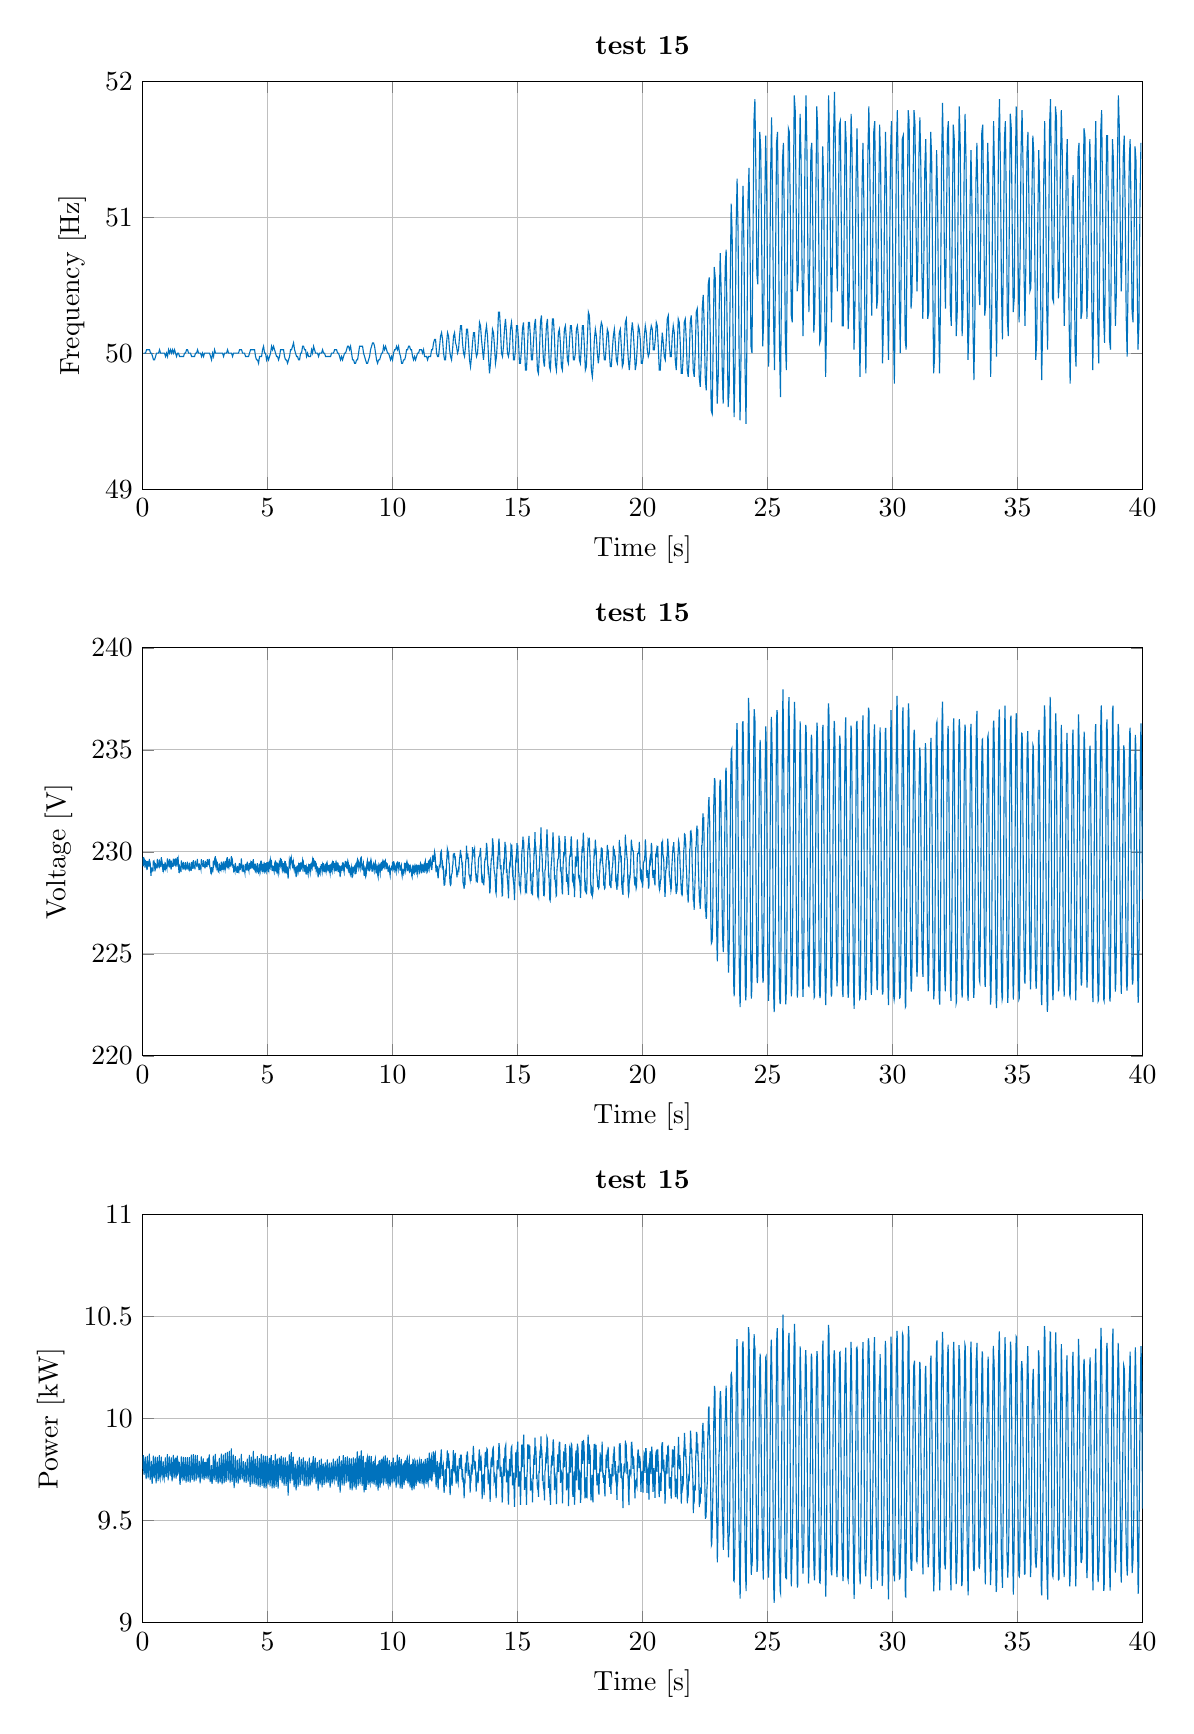
\begin{tikzpicture}

\begin{axis}[%
width=5in,
height=2.04in,
at={(1.135in,6.708in)},
scale only axis,
xmin=0,
xmax=40,
xlabel={Time [s]},
xmajorgrids,
ymajorgrids,
ymin=49,
ymax=52,
ylabel={Frequency [Hz]},
axis background/.style={fill=white},
title style={font=\bfseries},
title={test 15}
]
\addplot [color=mycolor1,solid,forget plot]
  table[row sep=crcr]{%
0.03996	50\\
0.07996	50\\
0.11996	50\\
0.15996	50.0250125062531\\
0.19994	50.0250125062531\\
0.23992	50.0250125062531\\
0.2799	50.0250125062531\\
0.31988	50\\
0.35988	50\\
0.39988	49.9750124937531\\
0.4399	49.9500499500499\\
0.47994	49.9500499500499\\
0.51998	49.9750124937532\\
0.56	50\\
0.6	50.0000000000001\\
0.64	50\\
0.68	50.0250125062531\\
0.71998	50\\
0.75998	50.0000000000001\\
0.79998	50\\
0.83998	50.0000000000001\\
0.87998	50\\
0.91998	49.9750124937531\\
0.96	50.0000000000001\\
1	49.9750124937531\\
1.04002	50.0250125062532\\
1.08	50\\
1.12	50.0250125062532\\
1.15998	50\\
1.19998	50.025012506253\\
1.23996	50\\
1.27996	50.0250125062532\\
1.31994	50\\
1.35994	49.9750124937532\\
1.39996	50\\
1.43996	50\\
1.47996	49.9750124937532\\
1.51998	49.9750124937532\\
1.56	49.9750124937532\\
1.60002	49.9750124937529\\
1.64004	49.9750124937532\\
1.68006	50\\
1.72006	50.0000000000002\\
1.76006	50.025012506253\\
1.80004	50.0250125062532\\
1.84002	50\\
1.88002	50\\
1.92002	50\\
1.96002	49.9750124937532\\
2.00004	49.9750124937529\\
2.04006	49.9750124937535\\
2.08008	49.9750124937529\\
2.1201	50\\
2.1601	50\\
2.2001	50.0250125062532\\
2.24008	50\\
2.28008	50\\
2.32008	50\\
2.36008	49.9750124937535\\
2.4001	50\\
2.4401	49.9750124937529\\
2.48012	50\\
2.52012	50\\
2.56012	50\\
2.60012	50.0000000000005\\
2.64012	50\\
2.68012	50\\
2.72012	49.9750124937529\\
2.76014	49.9500499500501\\
2.80018	50\\
2.84018	49.9750124937529\\
2.8802	50.0250125062532\\
2.92018	50\\
2.96018	50\\
3.00018	50\\
3.04018	50\\
3.08018	50.0000000000005\\
3.12018	50\\
3.16018	50\\
3.20018	50\\
3.24018	49.9750124937529\\
3.2802	50\\
3.3202	50\\
3.3602	50\\
3.4002	50.0250125062532\\
3.44018	50\\
3.48018	50\\
3.52018	50\\
3.56018	50.0000000000005\\
3.60018	49.9750124937529\\
3.6402	50\\
3.6802	50\\
3.7202	50\\
3.7602	50\\
3.8002	50\\
3.8402	50\\
3.8802	50.0250125062532\\
3.92018	50.0250125062532\\
3.96016	50.0250125062527\\
4.00014	50\\
4.04014	50.0000000000011\\
4.08014	50\\
4.12014	49.9750124937529\\
4.16016	49.9750124937529\\
4.20018	49.9750124937529\\
4.2402	49.9750124937529\\
4.28022	50\\
4.32022	50.0250125062532\\
4.3602	50.0250125062532\\
4.40018	50.0250125062532\\
4.44016	50.0250125062532\\
4.48014	50.0250125062532\\
4.52012	49.9750124937529\\
4.56014	49.9500499500496\\
4.60018	49.9500499500507\\
4.64022	49.9251123315022\\
4.68028	49.9750124937529\\
4.7203	49.975012493754\\
4.76032	49.9750124937529\\
4.80034	50.0250125062532\\
4.84032	50.0500500500492\\
4.88028	50\\
4.92028	50.0000000000011\\
4.96028	49.9500499500496\\
5.00032	49.9750124937529\\
5.04034	49.9500499500496\\
5.08038	49.975012493754\\
5.1204	50\\
5.1604	50.0500500500492\\
5.20036	50.0250125062532\\
5.24034	50.0500500500503\\
5.2803	50.0250125062532\\
5.32028	50\\
5.36028	49.9750124937529\\
5.4003	49.9750124937529\\
5.44032	49.9500499500507\\
5.48036	49.9750124937529\\
5.52038	50.0250125062532\\
5.56036	50.0250125062532\\
5.60034	50.0250125062532\\
5.64032	50.0250125062521\\
5.6803	49.975012493754\\
5.72032	49.9500499500496\\
5.76036	49.9500499500496\\
5.8004	49.9251123315033\\
5.84046	49.9500499500496\\
5.8805	49.9750124937529\\
5.92052	50.0250125062532\\
5.9605	50.0250125062532\\
6.00048	50.0500500500503\\
6.04044	50.0751126690028\\
6.08038	50.0250125062532\\
6.12036	50\\
6.16036	49.975012493754\\
6.20038	49.9750124937529\\
6.2404	49.9500499500496\\
6.28044	49.9500499500496\\
6.32048	50.0000000000011\\
6.36048	50\\
6.40048	50.0500500500492\\
6.44044	50.0500500500503\\
6.4804	50.0250125062532\\
6.52038	50.0250125062532\\
6.56036	49.9750124937529\\
6.60038	50\\
6.64038	49.9750124937529\\
6.6804	49.9750124937529\\
6.72042	49.975012493754\\
6.76044	50.0250125062532\\
6.80042	50\\
6.84042	50.0500500500492\\
6.88038	50.0250125062532\\
6.92036	50\\
6.96036	50\\
7.00036	50\\
7.04036	49.975012493754\\
7.08038	50\\
7.12038	50\\
7.16038	50\\
7.20038	50.0250125062532\\
7.24036	50\\
7.28036	50\\
7.32036	49.9750124937529\\
7.36038	49.9750124937529\\
7.4004	49.9750124937529\\
7.44042	49.9750124937529\\
7.48044	49.975012493754\\
7.52046	49.9750124937529\\
7.56048	50\\
7.60048	50\\
7.64048	50\\
7.68048	50.0250125062532\\
7.72046	50.0250125062532\\
7.76044	50.0250125062532\\
7.80042	50\\
7.84042	50\\
7.88042	49.9750124937529\\
7.92044	49.9500499500496\\
7.96048	49.975012493754\\
8.0005	49.9500499500485\\
8.04054	49.9750124937551\\
8.08056	49.9999999999988\\
8.12056	50.0000000000011\\
8.16056	50.025012506251\\
8.20054	50.0500500500514\\
8.2405	50.0500500500492\\
8.28046	50.0250125062532\\
8.32044	50.0500500500514\\
8.3604	49.9999999999988\\
8.4004	49.9500499500507\\
8.44044	49.9500499500485\\
8.48048	49.9251123315044\\
8.52054	49.9251123315022\\
8.5606	49.9500499500507\\
8.60064	49.9500499500485\\
8.64068	50.0000000000011\\
8.68068	50.0500500500492\\
8.72064	50.0500500500514\\
8.7606	50.0500500500492\\
8.80056	50.0500500500492\\
8.84052	50.0000000000011\\
8.88052	49.9750124937529\\
8.92054	49.9500499500507\\
8.96058	49.9251123315022\\
9.00064	49.9251123315022\\
9.0407	49.9500499500507\\
9.08074	49.9750124937529\\
9.12076	50.0250125062532\\
9.16074	50.0500500500492\\
9.2007	50.075112669004\\
9.24064	50.075112669004\\
9.28058	50.0500500500492\\
9.32054	50.0000000000011\\
9.36054	49.9500499500485\\
9.40058	49.9251123315044\\
9.44064	49.9500499500485\\
9.48068	49.9500499500507\\
9.52072	49.9750124937529\\
9.56074	50.0000000000011\\
9.60074	49.9999999999988\\
9.64074	50.0500500500492\\
9.6807	50.0250125062532\\
9.72068	50.0500500500514\\
9.76064	50.0250125062532\\
9.80062	49.9999999999988\\
9.84062	50.0000000000011\\
9.88062	49.9750124937529\\
9.92064	49.9500499500485\\
9.96068	49.9750124937551\\
10.0007	49.9500499500485\\
10.04074	50.0000000000011\\
10.08074	50.0250125062532\\
10.12072	50.0250125062532\\
10.1607	50.0500500500492\\
10.20066	50.0250125062532\\
10.24064	50.0500500500492\\
10.2806	50.0000000000011\\
10.3206	49.9750124937529\\
10.36062	49.9251123315022\\
10.40068	49.9251123315022\\
10.44074	49.9500499500507\\
10.48078	49.9500499500507\\
10.52082	49.9750124937529\\
10.56084	50.0250125062532\\
10.60082	50.0250125062532\\
10.6408	50.0500500500492\\
10.68076	50.0500500500514\\
10.72072	50.025012506251\\
10.7607	50.0250125062532\\
10.80068	49.9750124937551\\
10.8407	49.9500499500485\\
10.88074	49.9750124937529\\
10.92076	49.9500499500507\\
10.9608	49.9750124937529\\
11.00082	50.0000000000011\\
11.04082	49.9999999999988\\
11.08082	50.0250125062532\\
11.1208	50.0250125062532\\
11.16078	50.0250125062532\\
11.20076	49.9999999999988\\
11.24076	50.0250125062532\\
11.28074	49.9750124937551\\
11.32076	49.9750124937529\\
11.36078	49.9750124937529\\
11.4008	49.9500499500485\\
11.44084	49.9750124937529\\
11.48086	49.9750124937551\\
11.52088	49.9750124937529\\
11.5609	50.0250125062532\\
11.60088	50.0250125062532\\
11.64086	50.0751126690017\\
11.6808	50.1002004008033\\
11.72072	50.1002004008011\\
11.76064	49.9999999999988\\
11.80064	49.9750124937529\\
11.84066	49.9750124937551\\
11.88068	50.0500500500492\\
11.92064	50.1253132832088\\
11.96054	50.150451354062\\
12.00042	50.1002004008011\\
12.04034	49.9999999999988\\
12.08034	49.9500499500507\\
12.12038	49.9500499500507\\
12.16042	50.075112669004\\
12.20036	50.150451354062\\
12.24024	50.1253132832066\\
12.28014	50.0250125062532\\
12.32012	49.9750124937529\\
12.36014	49.9500499500507\\
12.40018	50.0250125062532\\
12.44016	50.1253132832088\\
12.48006	50.150451354062\\
12.51994	50.0751126690017\\
12.55988	50.0500500500514\\
12.59984	49.9999999999988\\
12.63984	50.0250125062532\\
12.67982	50.1253132832088\\
12.71972	50.2008032128516\\
12.75956	50.2008032128516\\
12.7994	50.075112669004\\
12.83934	49.9999999999988\\
12.87934	49.9750124937529\\
12.91936	50.0500500500514\\
12.95932	50.1756146512784\\
12.99918	50.1756146512806\\
13.03904	50.0751126690017\\
13.07898	49.9500499500507\\
13.11902	49.9001996007988\\
13.1591	49.9750124937529\\
13.19912	50.075112669004\\
13.23906	50.150451354062\\
13.27894	50.150451354062\\
13.31882	50.0250125062532\\
13.3588	49.9750124937529\\
13.39882	50.0000000000011\\
13.43882	50.1002004008011\\
13.47874	50.226017076845\\
13.51856	50.2008032128516\\
13.5584	50.1002004008011\\
13.59832	50.0250125062532\\
13.6383	49.9500499500507\\
13.67834	50.0500500500492\\
13.7183	50.150451354062\\
13.75818	50.2008032128516\\
13.79802	50.1253132832088\\
13.83792	49.9750124937529\\
13.87794	49.850448654038\\
13.91806	49.9251123315022\\
13.95812	50.0500500500514\\
13.99808	50.1756146512784\\
14.03794	50.150451354062\\
14.07782	50.0500500500514\\
14.11778	49.9251123315022\\
14.15784	49.9750124937529\\
14.19786	50.1002004008011\\
14.23778	50.301810865192\\
14.27754	50.3018108651897\\
14.3173	50.1756146512806\\
14.35716	49.9999999999988\\
14.39716	49.9750124937551\\
14.43718	50.0500500500492\\
14.47714	50.1756146512784\\
14.517	50.2512562814075\\
14.5568	50.150451354062\\
14.59668	50.0000000000011\\
14.63668	49.9750124937529\\
14.6767	50.0250125062532\\
14.71668	50.1756146512784\\
14.75654	50.2260170768472\\
14.79636	50.150451354062\\
14.83624	49.9500499500485\\
14.87628	49.9500499500507\\
14.91632	50.0250125062532\\
14.9563	50.2008032128516\\
14.99614	50.2008032128516\\
15.03598	50.1002004008011\\
15.0759	49.9251123315022\\
15.11596	49.9251123315044\\
15.15602	50.0250125062532\\
15.196	50.1756146512784\\
15.23586	50.226017076845\\
15.27568	50.075112669004\\
15.31562	49.8753117206996\\
15.35572	49.8753117206974\\
15.39582	50.0250125062532\\
15.4358	50.226017076845\\
15.47562	50.2260170768472\\
15.51544	50.1253132832066\\
15.55534	49.9500499500507\\
15.59538	49.9500499500507\\
15.63542	50.075112669004\\
15.67536	50.2008032128493\\
15.7152	50.2512562814075\\
15.755	50.075112669004\\
15.79494	49.8753117206974\\
15.83504	49.850448654038\\
15.87516	50.0000000000011\\
15.91516	50.226017076845\\
15.95498	50.2765208647557\\
15.99476	50.1002004008033\\
16.03468	49.9500499500485\\
16.07472	49.9001996007988\\
16.1148	50.0500500500492\\
16.15476	50.2008032128538\\
16.1946	50.2512562814075\\
16.2344	50.0751126690017\\
16.27434	49.9001996007988\\
16.31442	49.8753117206996\\
16.35452	50.0500500500492\\
16.39448	50.2512562814075\\
16.43428	50.2512562814075\\
16.47408	50.1253132832043\\
16.51398	49.9251123315066\\
16.55404	49.8753117206952\\
16.59414	50.0000000000011\\
16.63414	50.150451354062\\
16.67402	50.1756146512784\\
16.71388	50.0751126690062\\
16.75382	49.9001996007988\\
16.7939	49.8753117206952\\
16.834	50.0250125062532\\
16.87398	50.1756146512828\\
16.91384	50.2008032128493\\
16.95368	50.1002004008033\\
16.9936	49.9500499500485\\
17.03364	49.9251123315022\\
17.0737	50.0751126690017\\
17.11364	50.2008032128538\\
17.15348	50.2008032128493\\
17.19332	50.1002004008033\\
17.23324	49.9500499500485\\
17.27328	49.9500499500529\\
17.31332	49.9999999999966\\
17.35332	50.1756146512828\\
17.39318	50.2008032128493\\
17.43302	50.1253132832088\\
17.47292	49.9500499500485\\
17.51296	49.9251123315022\\
17.55302	50.0500500500537\\
17.59298	50.2008032128493\\
17.63282	50.2008032128538\\
17.67266	50.0500500500492\\
17.71262	49.8753117206952\\
17.75272	49.9001996007988\\
17.7928	50.1002004008033\\
17.83272	50.3018108651897\\
17.87248	50.2765208647557\\
17.91226	50.1253132832088\\
17.95216	49.8753117206996\\
17.99226	49.8256103637258\\
18.0324	49.9251123315022\\
18.07246	50.1002004008033\\
18.11238	50.1756146512784\\
18.15224	50.1253132832088\\
18.19214	50.0000000000011\\
18.23214	49.9251123315022\\
18.2722	50.0000000000011\\
18.3122	50.1756146512784\\
18.35206	50.2260170768472\\
18.39188	50.2008032128493\\
18.43172	50.0500500500492\\
18.47168	49.9500499500529\\
18.51172	49.9500499500485\\
18.55176	50.0751126690017\\
18.5917	50.1756146512828\\
18.63156	50.150451354062\\
18.67144	49.9999999999966\\
18.71144	49.9001996007988\\
18.75152	49.9001996007988\\
18.7916	50.0250125062532\\
18.83158	50.1253132832088\\
18.87148	50.1756146512784\\
18.91134	50.0751126690062\\
18.95128	49.9500499500485\\
18.99132	49.9251123315022\\
19.03138	50.0250125062532\\
19.07136	50.150451354062\\
19.11124	50.1756146512784\\
19.1511	50.0500500500537\\
19.19106	49.9001996007944\\
19.23114	49.9251123315066\\
19.2712	50.0751126690017\\
19.31114	50.2260170768472\\
19.35096	50.2512562814075\\
19.39076	50.0751126690017\\
19.4307	49.9500499500485\\
19.47074	49.8753117206996\\
19.51084	49.9750124937551\\
19.55086	50.150451354062\\
19.59074	50.2260170768428\\
19.63056	50.150451354062\\
19.67044	50.0250125062532\\
19.71042	49.8753117206996\\
19.75052	49.9251123315022\\
19.79058	50.0500500500492\\
19.83054	50.2008032128538\\
19.87038	50.1756146512784\\
19.91024	50.1002004008033\\
19.95016	49.9251123315022\\
19.99022	49.9251123314978\\
20.03028	49.9750124937507\\
20.0703	50.1253132832088\\
20.1102	50.2008032128538\\
20.15004	50.150451354062\\
20.18992	50.0250125062532\\
20.2299	49.9750124937507\\
20.26992	50.0000000000011\\
20.30992	50.150451354062\\
20.3498	50.2008032128538\\
20.38964	50.1756146512784\\
20.4295	50.0250125062532\\
20.46948	50.0250125062532\\
20.50946	50.1002004007989\\
20.54938	50.2260170768472\\
20.5892	50.2008032128493\\
20.62904	50.0500500500537\\
20.669	49.8753117206952\\
20.7091	49.8753117206996\\
20.7492	50.0250125062532\\
20.78918	50.150451354062\\
20.82906	50.0751126690017\\
20.869	49.9750124937551\\
20.90902	49.9500499500485\\
20.94906	50.1002004008033\\
20.98898	50.2512562814075\\
21.02878	50.2765208647557\\
21.06856	50.0751126690017\\
21.1085	49.9750124937551\\
21.14852	49.9750124937507\\
21.18854	50.1253132832088\\
21.22844	50.2008032128538\\
21.26828	50.150451354062\\
21.30816	49.9500499500485\\
21.3482	49.8753117206996\\
21.3883	50.0500500500492\\
21.42826	50.2512562814075\\
21.46806	50.2260170768472\\
21.50788	50.0751126690017\\
21.54782	49.8504486540358\\
21.58794	49.8504486540402\\
21.62806	49.9750124937507\\
21.66808	50.2260170768472\\
21.7079	50.2512562814075\\
21.7477	50.1002004008033\\
21.78762	49.8753117206952\\
21.82772	49.8256103637302\\
21.86786	49.9750124937507\\
21.90788	50.2260170768472\\
21.9477	50.2765208647557\\
21.98748	50.1253132832088\\
22.02738	49.8753117206952\\
22.06748	49.8256103637302\\
22.10762	50.0000000000011\\
22.14762	50.3018108651897\\
22.18738	50.3271263210847\\
22.22712	50.150451354062\\
22.267	49.8256103637302\\
22.30714	49.7512437810918\\
22.34734	49.9500499500529\\
22.38738	50.3271263210847\\
22.42712	50.4286434694935\\
22.46678	50.2008032128493\\
22.50662	49.8256103637258\\
22.54676	49.7265042267554\\
22.58698	50.0250125062532\\
22.62696	50.5050505050504\\
22.66656	50.5561172901901\\
22.70612	50.150451354062\\
22.746	49.5785820525527\\
22.78634	49.5540138751242\\
22.8267	50.0751126690062\\
22.86664	50.6329113924047\\
22.90614	50.5561172901901\\
22.9457	50.0500500500492\\
22.98566	49.6277915632773\\
23.02596	49.8256103637258\\
23.0661	50.3271263210892\\
23.10584	50.7356671740236\\
23.14526	50.4540867810266\\
23.1849	49.9001996007988\\
23.22498	49.6277915632773\\
23.26528	50.0500500500492\\
23.30524	50.6329113924047\\
23.34474	50.7614213197962\\
23.38414	50.1756146512784\\
23.424	49.6031746031774\\
23.46432	49.726504226751\\
23.50454	50.4540867810311\\
23.54418	51.0986203372512\\
23.58332	50.8905852417293\\
23.62262	50.0751126690017\\
23.66256	49.5294700346719\\
23.70294	49.9500499500485\\
23.74298	50.9164969450128\\
23.78226	51.2820512820493\\
23.82126	50.8905852417293\\
23.86056	50.0250125062532\\
23.90054	49.5049504950517\\
23.94094	50.0000000000011\\
23.98094	50.9164969450082\\
24.02022	51.2295081967214\\
24.05926	50.7356671740236\\
24.09868	49.9001996007988\\
24.13876	49.4804552201868\\
24.17918	50.1504513540665\\
24.21906	51.1247443762728\\
24.25818	51.3610683102253\\
24.29712	50.8388408744244\\
24.33646	50.0500500500492\\
24.37642	50.0000000000011\\
24.41642	50.8130081300832\\
24.45578	51.7063081695928\\
24.49446	51.8672199170167\\
24.53302	51.334702258723\\
24.57198	50.581689428433\\
24.61152	50.5050505050504\\
24.65112	51.072522982632\\
24.69028	51.6262261228695\\
24.72902	51.493305870241\\
24.76786	50.7614213197962\\
24.80726	50.0500500500492\\
24.84722	50.2512562814075\\
24.88702	51.0464522715648\\
24.9262	51.5995872033025\\
24.96496	51.2295081967214\\
25.004	50.4032258064508\\
25.04368	49.9001996007988\\
25.08376	50.4286434694889\\
25.12342	51.3347022587323\\
25.16238	51.7330574236936\\
25.20104	51.0986203372466\\
25.24018	50.2512562814075\\
25.27998	49.8753117206996\\
25.32008	50.6585612968578\\
25.35956	51.5463917525747\\
25.39836	51.6262261228743\\
25.4371	50.9424350483969\\
25.47636	50.0751126690017\\
25.5163	49.6770988574268\\
25.55656	50.4540867810266\\
25.5962	51.4138817480744\\
25.6351	51.5463917525747\\
25.6739	50.9164969450128\\
25.71318	50.0751126690017\\
25.75312	49.8753117206996\\
25.79322	50.7356671740236\\
25.83264	51.6528925619816\\
25.87136	51.6262261228743\\
25.9101	51.020408163264\\
25.9493	50.2765208647557\\
25.98908	50.2260170768472\\
26.0289	51.0986203372466\\
26.06804	51.8941359626395\\
26.10658	51.7866390471236\\
26.1452	51.0725229826367\\
26.18436	50.4540867810266\\
26.224	50.5305709954557\\
26.26358	51.282051282054\\
26.30258	51.7598343685288\\
26.34122	51.4138817480697\\
26.38012	50.6072874493933\\
26.41964	50.1253132832088\\
26.45954	50.6329113924047\\
26.49904	51.4933058702363\\
26.53788	51.8941359626395\\
26.57642	51.4933058702363\\
26.61526	50.6842372022278\\
26.65472	50.3018108651942\\
26.69448	50.735667174019\\
26.7339	51.493305870241\\
26.77274	51.5463917525747\\
26.81154	50.9164969450128\\
26.85082	50.1504513540575\\
26.8907	50.3018108651897\\
26.93046	51.1247443762821\\
26.96958	51.8134715025874\\
27.00818	51.6262261228743\\
27.04692	50.864699898266\\
27.08624	50.0751126690062\\
27.12618	50.1002004008033\\
27.1661	50.9164969450082\\
27.20538	51.5198351365307\\
27.2442	51.2557662737048\\
27.28322	50.4032258064508\\
27.3229	49.8256103637258\\
27.36304	50.2260170768472\\
27.40286	51.2820512820493\\
27.44186	51.8941359626347\\
27.4804	51.5463917525795\\
27.5192	50.7099391480743\\
27.55864	50.2260170768428\\
27.59846	50.7356671740236\\
27.63788	51.5463917525795\\
27.67668	51.9210799584606\\
27.7152	51.4933058702363\\
27.75404	50.7356671740236\\
27.79346	50.4540867810311\\
27.8331	51.0464522715648\\
27.87228	51.6795865633093\\
27.91098	51.7063081695975\\
27.94966	50.9683995922535\\
27.9889	50.2008032128538\\
28.02874	50.2008032128493\\
28.06858	50.9943906170318\\
28.1078	51.7063081695975\\
28.14648	51.5463917525795\\
28.18528	50.7356671740236\\
28.2247	50.1756146512739\\
28.26456	50.3778337531533\\
28.30426	51.308363263209\\
28.34324	51.7598343685288\\
28.38188	51.4668039114775\\
28.42074	50.6072874493933\\
28.46026	50.0250125062532\\
28.50024	50.3778337531488\\
28.53994	51.2820512820493\\
28.57894	51.6528925619863\\
28.61766	51.2032770097297\\
28.65672	50.3524672708929\\
28.69644	49.8256103637258\\
28.73658	50.2512562814075\\
28.77638	51.1770726714452\\
28.81546	51.5463917525747\\
28.85426	51.0986203372559\\
28.8934	50.2512562814075\\
28.9332	49.8504486540358\\
28.97332	50.47955577991\\
29.01294	51.4668039114775\\
29.0518	51.8134715025874\\
29.0904	51.3874614594073\\
29.12932	50.6072874493887\\
29.16884	50.2765208647557\\
29.20862	50.8130081300878\\
29.24798	51.6262261228648\\
29.28672	51.7063081695975\\
29.3254	51.0986203372512\\
29.36454	50.3271263210892\\
29.40428	50.4032258064508\\
29.44396	51.0725229826367\\
29.48312	51.6795865633046\\
29.52182	51.4138817480697\\
29.56072	50.6072874493978\\
29.60024	49.9251123314978\\
29.6403	50.2512562814075\\
29.6801	51.0986203372559\\
29.71924	51.6262261228648\\
29.75798	51.2032770097297\\
29.79704	50.3778337531533\\
29.83674	49.9500499500485\\
29.87678	50.5561172901901\\
29.91634	51.4403292181084\\
29.95522	51.7063081695975\\
29.9939	51.0725229826367\\
30.03306	50.2008032128493\\
30.0729	49.776007964162\\
30.11308	50.4795557799055\\
30.1527	51.4933058702363\\
30.19154	51.7866390471284\\
30.23016	51.282051282054\\
30.26916	50.4540867810266\\
30.3088	50.0000000000011\\
30.3488	50.6842372022278\\
30.38826	51.5729757607025\\
30.42704	51.5995872033025\\
30.4658	50.8646998982706\\
30.50512	50.1002004008033\\
30.54504	50.0250125062532\\
30.58502	50.8905852417293\\
30.62432	51.7866390471284\\
30.66294	51.7063081695975\\
30.70162	50.9683995922488\\
30.74086	50.3271263210892\\
30.7806	50.4540867810311\\
30.82024	51.2557662737048\\
30.85926	51.7866390471236\\
30.89788	51.6795865633093\\
30.93658	50.9683995922535\\
30.97582	50.4540867810266\\
31.01546	50.7356671740236\\
31.05488	51.4403292181037\\
31.09376	51.7330574236936\\
31.13242	51.3610683102253\\
31.17136	50.6329113924047\\
31.21086	50.2512562814075\\
31.25066	50.6585612968578\\
31.29014	51.3610683102206\\
31.32908	51.5729757607025\\
31.36786	51.020408163264\\
31.40706	50.2512562814075\\
31.44686	50.3018108651897\\
31.48662	51.0464522715695\\
31.5258	51.6262261228695\\
31.56454	51.4403292181084\\
31.60342	50.6329113924047\\
31.64292	49.8504486540402\\
31.68304	49.9750124937507\\
31.72306	50.8905852417293\\
31.76236	51.4933058702363\\
31.8012	51.150895140668\\
31.8403	50.3271263210847\\
31.88004	49.8504486540358\\
31.92016	50.4032258064554\\
31.95984	51.3610683102206\\
31.99878	51.8403317781239\\
32.03736	51.4403292181084\\
32.07624	50.6842372022232\\
32.1157	50.3271263210937\\
32.15544	50.9164969450036\\
32.19472	51.6262261228743\\
32.23346	51.7063081695975\\
32.27214	51.1247443762728\\
32.31126	50.3271263210937\\
32.351	50.2008032128538\\
32.39084	50.9943906170318\\
32.43006	51.6795865632998\\
32.46876	51.5729757607073\\
32.50754	50.7356671740236\\
32.54696	50.1253132832043\\
32.58686	50.3018108651897\\
32.62662	51.1770726714452\\
32.6657	51.8134715025874\\
32.7043	51.5729757607073\\
32.74308	50.7356671740236\\
32.7825	50.1253132832043\\
32.8224	50.3524672708929\\
32.86212	51.3083632632183\\
32.9011	51.7598343685288\\
32.93974	51.4138817480744\\
32.97864	50.5561172901901\\
33.0182	49.9500499500529\\
33.05824	50.2008032128448\\
33.09808	51.0725229826413\\
33.13724	51.4933058702363\\
33.17608	51.0986203372466\\
33.21522	50.2260170768472\\
33.25504	49.8007968127488\\
33.2952	50.3018108651897\\
33.33496	51.2557662737048\\
33.37398	51.5463917525842\\
33.41278	51.1508951406587\\
33.45188	50.47955577991\\
33.4915	50.3524672709019\\
33.53122	50.8905852417247\\
33.57052	51.6262261228743\\
33.60926	51.6795865633093\\
33.64796	51.020408163264\\
33.68716	50.2765208647557\\
33.72694	50.3524672708929\\
33.76666	50.9683995922535\\
33.8059	51.5463917525747\\
33.8447	51.2820512820587\\
33.8837	50.4286434694844\\
33.92336	49.8256103637258\\
33.9635	50.2008032128538\\
34.00334	51.1247443762821\\
34.04246	51.7063081695975\\
34.08114	51.2820512820493\\
34.12014	50.4540867810311\\
34.15978	49.9750124937463\\
34.1998	50.6072874493978\\
34.23932	51.5729757606978\\
34.2781	51.8672199170167\\
34.31666	51.334702258723\\
34.35562	50.47955577991\\
34.39524	50.1002004007989\\
34.43516	50.7356671740236\\
34.47458	51.5729757607073\\
34.51336	51.7063081695975\\
34.55204	51.072522982632\\
34.5912	50.2512562814075\\
34.631	50.1253132832043\\
34.6709	50.9424350483969\\
34.71016	51.7598343685288\\
34.7488	51.6528925619863\\
34.78752	50.9164969450128\\
34.8268	50.3018108651897\\
34.86656	50.4032258064554\\
34.90624	51.2557662737048\\
34.94526	51.8134715025874\\
34.98386	51.4933058702363\\
35.0227	50.6585612968624\\
35.06218	50.2260170768383\\
35.102	50.6842372022323\\
35.14146	51.4933058702363\\
35.1803	51.7866390471332\\
35.21892	51.387461459398\\
35.25784	50.6072874493978\\
35.29736	50.2008032128448\\
35.3372	50.7099391480743\\
35.37664	51.4668039114775\\
35.4155	51.6262261228743\\
35.45424	51.1247443762728\\
35.49336	50.4540867810311\\
35.533	50.47955577991\\
35.57262	51.1247443762821\\
35.61174	51.5995872032978\\
35.6505	51.4668039114775\\
35.68936	50.7356671740236\\
35.72878	49.9500499500529\\
35.76882	50.1002004007989\\
35.80874	50.9424350483969\\
35.848	51.4933058702363\\
35.88684	51.1770726714452\\
35.92592	50.3778337531443\\
35.96562	49.8007968127488\\
36.00578	50.2260170768472\\
36.0456	51.2295081967214\\
36.08464	51.7063081695975\\
36.12332	51.2032770097297\\
36.16238	50.3778337531443\\
36.20208	50.0250125062532\\
36.24206	50.7356671740236\\
36.28148	51.6795865633093\\
36.32018	51.8672199170167\\
36.35874	51.2032770097203\\
36.3978	50.4032258064554\\
36.43748	50.3778337531533\\
36.47718	51.1508951406587\\
36.51628	51.813471502597\\
36.55488	51.7330574236936\\
36.59354	51.020408163264\\
36.63274	50.4032258064463\\
36.67242	50.5305709954512\\
36.712	51.3347022587323\\
36.75096	51.7866390471236\\
36.78958	51.4668039114775\\
36.82844	50.6842372022323\\
36.8679	50.2008032128448\\
36.90774	50.581689428433\\
36.94728	51.334702258723\\
36.98624	51.5729757607073\\
37.02502	51.0986203372466\\
37.06416	50.2260170768472\\
37.10398	49.776007964162\\
37.14416	50.2765208647557\\
37.18394	51.1247443762728\\
37.22306	51.3083632632183\\
37.26204	50.7872016251888\\
37.30142	50.0250125062532\\
37.3414	49.9001996007944\\
37.38148	50.6072874493978\\
37.421	51.4668039114775\\
37.45986	51.5463917525747\\
37.49866	50.9164969450128\\
37.53794	50.2512562814075\\
37.57774	50.3018108651897\\
37.6175	50.9683995922535\\
37.65674	51.6528925619863\\
37.69546	51.5995872032978\\
37.73422	50.8905852417339\\
37.77352	50.2512562814075\\
37.81332	50.5050505050504\\
37.85292	51.2032770097203\\
37.89198	51.5729757607073\\
37.93076	51.2032770097297\\
37.96982	50.3778337531443\\
38.00952	49.875311720704\\
38.04962	50.4286434694844\\
38.08928	51.3347022587323\\
38.12824	51.7063081695975\\
38.16692	51.072522982632\\
38.20608	50.2512562814075\\
38.24588	49.9251123315066\\
38.28594	50.7099391480651\\
38.32538	51.6262261228743\\
38.36412	51.7866390471236\\
38.40274	51.1247443762821\\
38.44186	50.2765208647557\\
38.48164	50.0751126690017\\
38.52158	50.8388408744244\\
38.56092	51.5995872033072\\
38.59968	51.5995872032978\\
38.63844	50.8905852417339\\
38.67774	50.1002004007989\\
38.71766	50.0250125062532\\
38.75764	50.8905852417339\\
38.79694	51.5729757606978\\
38.83572	51.4138817480744\\
38.87462	50.7099391480743\\
38.91406	50.2008032128538\\
38.9539	50.454086781022\\
38.99354	51.3610683102253\\
39.03248	51.8941359626395\\
39.07102	51.6528925619768\\
39.10974	50.8905852417339\\
39.14904	50.4540867810311\\
39.18868	50.7872016251888\\
39.22806	51.4403292181084\\
39.26694	51.5995872032978\\
39.3057	51.0725229826413\\
39.34486	50.2765208647557\\
39.38464	49.9750124937463\\
39.42466	50.581689428433\\
39.4642	51.387461459398\\
39.50312	51.5729757607073\\
39.5419	51.0464522715648\\
39.58108	50.3018108651897\\
39.62084	50.2260170768472\\
39.66066	50.8388408744244\\
39.7	51.5198351365354\\
39.73882	51.413881748065\\
39.77772	50.6842372022323\\
39.81718	50.0250125062532\\
39.85716	50.2260170768472\\
39.89698	51.0986203372466\\
39.93612	51.5463917525842\\
};
\end{axis}

\begin{axis}[%
width=5in,
height=2.04in,
at={(1.135in,3.874in)},
scale only axis,
xmin=0,
xmax=40,
xlabel={Time [s]},
xmajorgrids,
ymajorgrids,
ymin=220,
ymax=240,
ylabel={Voltage [V]},
axis background/.style={fill=white},
title style={font=\bfseries},
title={test 15}
]
\addplot [color=mycolor1,solid,forget plot]
  table[row sep=crcr]{%
0.016	229.306449672573\\
0.032	229.746342837692\\
0.048	229.507176927047\\
0.064	229.655691494273\\
0.08	229.604321737178\\
0.096	229.234989788523\\
0.112	229.610720493787\\
0.128	229.439562284547\\
0.144	229.470201929611\\
0.16	229.300514705524\\
0.176	229.115270957138\\
0.192	229.550161688938\\
0.208	229.349559252369\\
0.224	229.482409981979\\
0.24	229.441435268986\\
0.256	229.280169935345\\
0.272	229.65101518527\\
0.288	229.449494276456\\
0.304	229.469879864229\\
0.32	229.212395837647\\
0.336	228.82799652631\\
0.352	229.196988947119\\
0.368	228.996958482635\\
0.384	229.194635547402\\
0.4	229.172932962792\\
0.416	229.05140166044\\
0.432	229.58325301339\\
0.448	229.43937733064\\
0.464	229.507442531244\\
0.48	229.39711989553\\
0.496	229.053095025375\\
0.512	229.464724258605\\
0.528	229.252486696658\\
0.544	229.351180913914\\
0.56	229.321048543162\\
0.576	229.19688663308\\
0.592	229.661026102741\\
0.608	229.358995630919\\
0.624	229.438154303285\\
0.64	229.421276644149\\
0.656	229.235682728101\\
0.672	229.634162198526\\
0.688	229.366525346255\\
0.704	229.47577594823\\
0.72	229.430436723942\\
0.736	229.259938076304\\
0.752	229.748092785266\\
0.768	229.431469113026\\
0.784	229.493458964553\\
0.8	229.353684336085\\
0.816	229.01732856584\\
0.832	229.408969901818\\
0.848	229.138778050024\\
0.864	229.234501551158\\
0.88	229.33207444752\\
0.896	229.113589412607\\
0.912	229.486696019412\\
0.928	229.232703554723\\
0.944	229.331172981013\\
0.96	229.302496696761\\
0.976	229.202464641104\\
0.992	229.676574696869\\
1.008	229.401473000549\\
1.024	229.492198326827\\
1.04	229.453627999169\\
1.056	229.251823682577\\
1.072	229.659356677772\\
1.088	229.412390944826\\
1.104	229.521481213337\\
1.12	229.437864386972\\
1.136	229.141575311066\\
1.152	229.572141307125\\
1.168	229.322104593692\\
1.184	229.421997786998\\
1.2	229.417930018194\\
1.216	229.274479597633\\
1.232	229.670009616697\\
1.248	229.459929418014\\
1.264	229.57041247593\\
1.28	229.523794007632\\
1.296	229.314004597836\\
1.312	229.682835285218\\
1.328	229.446213515567\\
1.344	229.558911221628\\
1.36	229.485939867854\\
1.376	229.275836245632\\
1.392	229.748165255012\\
1.408	229.535806612659\\
1.424	229.651089748334\\
1.44	229.389397573426\\
1.456	228.976067245978\\
1.472	229.385475862519\\
1.488	229.135613288684\\
1.504	229.243530684887\\
1.52	229.204865740919\\
1.536	229.016431698821\\
1.552	229.584205350375\\
1.568	229.328076273577\\
1.584	229.386913434822\\
1.6	229.339451053937\\
1.616	229.137690092501\\
1.632	229.514465232323\\
1.648	229.252766090547\\
1.664	229.313480751356\\
1.68	229.284206691484\\
1.696	229.130241821432\\
1.712	229.495957164985\\
1.728	229.251964683508\\
1.744	229.342022901904\\
1.76	229.333176206856\\
1.776	229.134926463148\\
1.792	229.518596720009\\
1.808	229.256838563153\\
1.824	229.305377853065\\
1.84	229.287783433499\\
1.856	229.084011491291\\
1.872	229.467959957591\\
1.888	229.172162663089\\
1.904	229.248377690868\\
1.92	229.250251626503\\
1.936	229.068404687058\\
1.952	229.501184178345\\
1.968	229.281860028938\\
1.984	229.414049002895\\
2	229.350667840956\\
2.016	229.165945409077\\
2.032	229.598862718371\\
2.048	229.293371820756\\
2.064	229.337001230744\\
2.08	229.320725827613\\
2.096	229.141927229057\\
2.112	229.57344311446\\
2.128	229.365339074218\\
2.144	229.376735861722\\
2.16	229.400435029737\\
2.176	229.252321652729\\
2.192	229.65645731893\\
2.208	229.377124377265\\
2.224	229.402516609257\\
2.24	229.396362288775\\
2.256	229.108429825766\\
2.272	229.43863243288\\
2.288	229.161713667323\\
2.304	229.179335109803\\
2.32	229.262484258735\\
2.336	229.157368370136\\
2.352	229.639819319589\\
2.368	229.422036448805\\
2.384	229.398424559449\\
2.4	229.407229708102\\
2.416	229.25361817898\\
2.432	229.598995841727\\
2.448	229.302101727037\\
2.464	229.288984208125\\
2.48	229.343087852954\\
2.496	229.19656934898\\
2.512	229.56198946082\\
2.528	229.291559988589\\
2.544	229.312227178151\\
2.56	229.39352848719\\
2.576	229.258391243019\\
2.592	229.643726414193\\
2.608	229.383102305601\\
2.624	229.390725236566\\
2.64	229.491755520677\\
2.656	229.343506182994\\
2.672	229.661264078858\\
2.688	229.28930191374\\
2.704	229.175292365601\\
2.72	229.136649211496\\
2.736	228.915855255236\\
2.752	229.253919078617\\
2.768	228.98493452135\\
2.784	229.047168487059\\
2.8	229.158033696389\\
2.816	229.110557534549\\
2.832	229.571933385843\\
2.848	229.335048514672\\
2.864	229.422444884365\\
2.88	229.58027625342\\
2.896	229.49591857445\\
2.912	229.790787926871\\
2.928	229.306660340254\\
2.944	229.223667268182\\
2.96	229.421000457092\\
2.976	229.236096593188\\
2.992	229.523837971182\\
3.008	229.136980729756\\
3.024	229.068026710123\\
3.04	229.136872209361\\
3.056	229.071946282693\\
3.072	229.441710055271\\
3.088	229.140360415541\\
3.104	229.114785665213\\
3.12	229.232798355945\\
3.136	229.162579766558\\
3.152	229.521095971114\\
3.168	229.144451818089\\
3.184	229.157822062049\\
3.2	229.295828785448\\
3.216	229.20064558685\\
3.232	229.532718668408\\
3.248	229.1546086417\\
3.264	229.159240710376\\
3.28	229.319975161537\\
3.296	229.191553941998\\
3.312	229.562402925845\\
3.328	229.234029627238\\
3.344	229.309589371815\\
3.36	229.519971424874\\
3.376	229.410845736148\\
3.392	229.737380271501\\
3.408	229.40630414199\\
3.424	229.284346940392\\
3.44	229.405488736158\\
3.456	229.322091780046\\
3.472	229.675067837422\\
3.488	229.31699923703\\
3.504	229.300889502295\\
3.52	229.416453492658\\
3.536	229.377279516963\\
3.552	229.790943927967\\
3.568	229.38990002281\\
3.584	229.371979728515\\
3.6	229.496459717026\\
3.616	229.202490450493\\
3.632	229.388981620506\\
3.648	229.048698140053\\
3.664	229.074599701081\\
3.68	229.209127686438\\
3.696	229.097906782437\\
3.712	229.465325840512\\
3.728	229.175090469884\\
3.744	229.114622599201\\
3.76	229.16648992776\\
3.776	228.975290290853\\
3.792	229.313996485504\\
3.808	229.027897961576\\
3.824	229.006639823558\\
3.84	229.171610744528\\
3.856	229.101345813913\\
3.872	229.451476307912\\
3.888	229.132269359259\\
3.904	229.146614878089\\
3.92	229.302580349326\\
3.936	229.221389207184\\
3.952	229.682819002649\\
3.968	229.368371912281\\
3.984	229.254832480799\\
4	229.165708654066\\
4.016	229.008622888054\\
4.032	229.373456294322\\
4.048	229.078124075158\\
4.064	229.060868604227\\
4.08	229.084368521531\\
4.096	228.969672151191\\
4.112	229.407186342501\\
4.128	229.181724967914\\
4.144	229.150712436778\\
4.16	229.312045877107\\
4.176	229.238410395287\\
4.192	229.519762559487\\
4.208	229.195353435217\\
4.224	229.14983701376\\
4.24	229.239677870738\\
4.256	229.110431602343\\
4.272	229.465360101114\\
4.288	229.173557602642\\
4.304	229.187773315258\\
4.32	229.369375351301\\
4.336	229.179623636554\\
4.352	229.55066891057\\
4.368	229.285815528532\\
4.384	229.259865502884\\
4.4	229.410637804609\\
4.416	229.31704949116\\
4.432	229.639371518505\\
4.448	229.259220408182\\
4.464	229.199444172516\\
4.48	229.288729390605\\
4.496	229.166381137016\\
4.512	229.428228196107\\
4.528	229.051701988801\\
4.544	229.020166423948\\
4.56	229.193789790174\\
4.576	229.137860822502\\
4.592	229.452824215883\\
4.608	229.122495726792\\
4.624	229.038102144895\\
4.64	229.121094243622\\
4.656	229.02084278886\\
4.672	229.422982932686\\
4.688	229.195724969521\\
4.704	229.081235892696\\
4.72	229.368457628765\\
4.736	229.254616720589\\
4.752	229.565651825352\\
4.768	229.288294401765\\
4.784	229.156007725443\\
4.8	229.412235670944\\
4.816	229.211146353709\\
4.832	229.312515192206\\
4.848	229.056958540587\\
4.864	229.019033489347\\
4.88	229.309816735314\\
4.896	229.190681156163\\
4.912	229.453892481077\\
4.928	229.079896171629\\
4.944	229.022788348341\\
4.96	229.331839875216\\
4.976	229.260288339462\\
4.992	229.499692735364\\
5.008	229.176187984938\\
5.024	229.013906626208\\
5.04	229.300730337947\\
5.056	229.15441115639\\
5.072	229.401520836152\\
5.088	229.244416966368\\
5.104	229.205806748706\\
5.12	229.571517859232\\
5.136	229.440119485923\\
5.152	229.613054766173\\
5.168	229.287456977236\\
5.184	229.055656731849\\
5.2	229.343387175416\\
5.216	229.069666968444\\
5.232	229.314202670681\\
5.248	229.117621027895\\
5.264	229.028716284402\\
5.28	229.302940091516\\
5.296	229.219606263051\\
5.312	229.580561812392\\
5.328	229.235260241873\\
5.344	229.122061341683\\
5.36	229.315425057702\\
5.376	229.176552579163\\
5.392	229.474641368243\\
5.408	229.072446176448\\
5.424	228.951166311932\\
5.44	229.23008842513\\
5.456	229.120723775183\\
5.472	229.517982516842\\
5.488	229.477731225452\\
5.504	229.373264909114\\
5.52	229.706435364789\\
5.536	229.508126714398\\
5.552	229.64242953106\\
5.568	229.285613029319\\
5.584	229.155837727808\\
5.6	229.336170714338\\
5.616	229.198085938451\\
5.632	229.447228318945\\
5.648	229.132546681723\\
5.664	229.072557037123\\
5.68	229.349015496572\\
5.696	229.213110255651\\
5.712	229.550505935964\\
5.728	229.135071202158\\
5.744	228.945138810385\\
5.76	229.21364988278\\
5.776	229.094290376044\\
5.792	229.28115946087\\
5.808	228.920950871469\\
5.824	228.694309503008\\
5.84	229.161647908732\\
5.856	229.194579199873\\
5.872	229.573104157987\\
5.888	229.442249109709\\
5.904	229.317771653096\\
5.92	229.629344702171\\
5.936	229.567156652668\\
5.952	229.692497246634\\
5.968	229.485187329832\\
5.984	229.373367230641\\
6	229.57990355045\\
6.016	229.391389714425\\
6.032	229.508355237764\\
6.048	229.227343372392\\
6.064	229.121902599037\\
6.08	229.374716960072\\
6.096	229.091797403043\\
6.112	229.266046008444\\
6.128	228.975739083147\\
6.144	228.763146648383\\
6.16	229.102694965164\\
6.176	229.01981865615\\
6.192	229.334062439141\\
6.208	229.183024132337\\
6.224	229.062117144811\\
6.24	229.309347180811\\
6.256	229.200177114825\\
6.272	229.454052049086\\
6.288	229.220281439694\\
6.304	229.028106051181\\
6.32	229.346903020007\\
6.336	229.274462486897\\
6.352	229.478352103916\\
6.368	229.262101823184\\
6.384	229.190149147136\\
6.4	229.538458643259\\
6.416	229.406846532484\\
6.432	229.481809912044\\
6.448	229.223299540629\\
6.464	229.007583810531\\
6.48	229.363181539174\\
6.496	229.144866884428\\
6.512	229.350060516254\\
6.528	229.036494721614\\
6.544	228.889753983931\\
6.56	229.209656789951\\
6.576	229.089780275352\\
6.592	229.27007366257\\
6.608	229.05684682911\\
6.624	228.925967661888\\
6.64	229.281178855779\\
6.656	229.21150004769\\
6.672	229.402295445378\\
6.688	229.107797701461\\
6.704	228.979697641627\\
6.72	229.262647761063\\
6.736	229.16877386952\\
6.752	229.346058626901\\
6.768	229.245203252434\\
6.784	229.193864209974\\
6.8	229.564278868916\\
6.816	229.450898242898\\
6.832	229.700847183986\\
6.848	229.460818461204\\
6.864	229.276267363427\\
6.88	229.580924125248\\
6.896	229.372368806337\\
6.912	229.545134281882\\
6.928	229.320681673916\\
6.944	229.107625742756\\
6.96	229.251354403118\\
6.976	229.037445786106\\
6.992	229.292929867263\\
7.008	228.987825184742\\
7.024	228.759432896792\\
7.04	229.084519267498\\
7.056	229.010809293013\\
7.072	229.214980463503\\
7.088	229.020376345448\\
7.104	228.951090433026\\
7.12	229.306780432646\\
7.136	229.142693883077\\
7.152	229.402358743925\\
7.168	229.165178764479\\
7.184	229.0307006159\\
7.2	229.327942721091\\
7.216	229.217852931901\\
7.232	229.445991078364\\
7.248	229.217615864419\\
7.264	229.006935703869\\
7.28	229.32595705038\\
7.296	229.171540181599\\
7.312	229.419977970093\\
7.328	229.250942732823\\
7.344	229.098366863211\\
7.36	229.343884450663\\
7.376	229.221634658506\\
7.392	229.38855633906\\
7.408	229.251084297134\\
7.424	229.058269646948\\
7.44	229.350741792186\\
7.456	229.186717921743\\
7.472	229.369848964672\\
7.488	229.096175776175\\
7.504	228.952985050223\\
7.52	229.227528420552\\
7.536	229.129274102655\\
7.552	229.308334459383\\
7.568	229.187974475759\\
7.584	229.079579204475\\
7.6	229.44686771762\\
7.616	229.373961614263\\
7.632	229.544119180636\\
7.648	229.236366370677\\
7.664	229.120544995536\\
7.68	229.313181294585\\
7.696	229.220277307226\\
7.712	229.372855917618\\
7.728	229.180981435562\\
7.744	229.045152467545\\
7.76	229.399504229725\\
7.776	229.300711357416\\
7.792	229.485356982822\\
7.808	229.189075395737\\
7.824	229.01718584286\\
7.84	229.284959118715\\
7.856	229.178052763417\\
7.872	229.342872066588\\
7.888	229.012924541022\\
7.904	228.761171415993\\
7.92	229.153537686673\\
7.936	229.090886658903\\
7.952	229.339213626325\\
7.968	229.092231665966\\
7.984	229.096701424772\\
8	229.452202045009\\
8.016	229.433410161912\\
8.032	229.442613310258\\
8.048	229.103809461648\\
8.064	229.007896485445\\
8.08	229.362542264765\\
8.096	229.384175416038\\
8.112	229.554402210634\\
8.128	229.309861911668\\
8.144	229.264469086403\\
8.16	229.403866188573\\
8.176	229.32695792812\\
8.192	229.474794273034\\
8.208	229.254098238241\\
8.224	229.150815555536\\
8.24	229.358726465286\\
8.256	229.190717967636\\
8.272	229.360706044364\\
8.288	229.037916290656\\
8.304	228.941440237998\\
8.32	229.224870500523\\
8.336	229.069225224332\\
8.352	229.218601163114\\
8.368	228.974889566288\\
8.384	228.716530860734\\
8.4	229.081868170803\\
8.416	228.988671457531\\
8.432	229.272832176393\\
8.448	229.085545954639\\
8.464	229.023461556197\\
8.48	229.236581118499\\
8.496	229.170986197192\\
8.512	229.2714991491\\
8.528	228.946799277332\\
8.544	228.958833359935\\
8.56	229.44625528583\\
8.576	229.491535395074\\
8.592	229.583490294544\\
8.608	229.28344756531\\
8.624	229.201145675596\\
8.64	229.527183055144\\
8.656	229.478566555183\\
8.672	229.455869870999\\
8.688	229.258910534405\\
8.704	229.177804706764\\
8.72	229.637289596618\\
8.736	229.724371312291\\
8.752	229.742036099851\\
8.768	229.338104858516\\
8.784	229.102641949685\\
8.8	229.360378409243\\
8.816	229.329129895688\\
8.832	229.428329115962\\
8.848	229.090607637681\\
8.864	228.832351060423\\
8.88	229.11019972251\\
8.896	228.97849139046\\
8.912	229.091554872613\\
8.928	228.793119295124\\
8.944	228.857546735395\\
8.96	229.267161270601\\
8.976	229.459203348581\\
8.992	229.560032017335\\
9.008	229.225574400513\\
9.024	229.065632272132\\
9.04	229.454469464452\\
9.056	229.501611158042\\
9.072	229.469438805904\\
9.088	229.106488705117\\
9.104	229.139761361534\\
9.12	229.533457913085\\
9.136	229.629837476499\\
9.152	229.521422500126\\
9.168	229.192451579943\\
9.184	229.024430864893\\
9.2	229.281640014314\\
9.216	229.310507096489\\
9.232	229.389557657647\\
9.248	229.160148310115\\
9.264	229.067607850684\\
9.28	229.373627471568\\
9.296	229.427353884991\\
9.312	229.491245934509\\
9.328	229.159497128446\\
9.344	228.954360543823\\
9.36	229.216384337787\\
9.376	229.096773935904\\
9.392	229.201180296274\\
9.408	228.860090258315\\
9.424	228.768049139537\\
9.44	229.263702521559\\
9.456	229.399602094731\\
9.472	229.352296994938\\
9.488	229.067127567466\\
9.504	228.942383898056\\
9.52	229.353599893499\\
9.536	229.447304519565\\
9.552	229.465886167544\\
9.568	229.111551048966\\
9.584	229.11907607359\\
9.6	229.494432147115\\
9.616	229.580388360044\\
9.632	229.530424053688\\
9.648	229.235257055548\\
9.664	229.207277180422\\
9.68	229.544295237803\\
9.696	229.541128951802\\
9.712	229.581084346232\\
9.728	229.30854625322\\
9.744	229.145414332124\\
9.76	229.450594070948\\
9.776	229.433867117919\\
9.792	229.409313328359\\
9.808	229.195399704849\\
9.824	229.010442841913\\
9.84	229.239908561833\\
9.856	229.253504266852\\
9.872	229.285988290923\\
9.888	228.979486452651\\
9.904	228.848418495901\\
9.92	229.129388708913\\
9.936	229.192271968919\\
9.952	229.243965173924\\
9.968	229.147998808161\\
9.984	229.114849386693\\
10	229.4794596102\\
10.016	229.498536390735\\
10.032	229.509265252805\\
10.048	229.138155847462\\
10.064	229.084577922347\\
10.08	229.372638841601\\
10.096	229.299497931202\\
10.112	229.293110890965\\
10.128	229.097653257747\\
10.144	229.009717308655\\
10.16	229.406523023078\\
10.176	229.463258143914\\
10.192	229.486587003272\\
10.208	229.23609877413\\
10.224	229.129283409685\\
10.24	229.405821652516\\
10.256	229.485701047628\\
10.272	229.479826314571\\
10.288	229.268848354274\\
10.304	229.075851005386\\
10.32	229.294905437011\\
10.336	229.27840083259\\
10.352	229.341253285878\\
10.368	228.952317989583\\
10.384	228.825796011998\\
10.4	229.068441328739\\
10.416	229.122423173703\\
10.432	229.094945383635\\
10.448	228.944680022291\\
10.464	229.022733901097\\
10.48	229.4420969404\\
10.496	229.435435254627\\
10.512	229.408312091802\\
10.528	229.07891512568\\
10.544	229.172781635105\\
10.56	229.453349997353\\
10.576	229.533006459368\\
10.592	229.435402165177\\
10.608	229.084014694132\\
10.624	229.078183504011\\
10.64	229.369066761683\\
10.656	229.334565397971\\
10.672	229.33651578432\\
10.688	229.027421658549\\
10.704	229.062136334259\\
10.72	229.250282474856\\
10.736	229.156948394121\\
10.752	229.091124367012\\
10.768	228.835395636223\\
10.784	228.767605065537\\
10.8	229.274305201812\\
10.816	229.334833685952\\
10.832	229.312993001388\\
10.848	228.958290140949\\
10.864	228.931436039904\\
10.88	229.260857833778\\
10.896	229.336748486429\\
10.912	229.249118657634\\
10.928	229.035219846538\\
10.944	228.986632405592\\
10.96	229.355230650278\\
10.976	229.35089047043\\
10.992	229.29795148977\\
11.008	228.95466569784\\
11.024	229.081078203236\\
11.04	229.340526503744\\
11.056	229.336577710932\\
11.072	229.282130698318\\
11.088	228.993562955547\\
11.104	229.040280363546\\
11.12	229.448884447468\\
11.136	229.403364451919\\
11.152	229.372027109838\\
11.168	229.003003939826\\
11.184	229.027069051959\\
11.2	229.353801359267\\
11.216	229.379880305696\\
11.232	229.295460218896\\
11.248	229.017929056879\\
11.264	229.008166547126\\
11.28	229.374616358409\\
11.296	229.483576095946\\
11.312	229.553696359589\\
11.328	229.091540841965\\
11.344	229.039284899493\\
11.36	229.352014296\\
11.376	229.430837619485\\
11.392	229.425499499354\\
11.408	229.063727265957\\
11.424	229.117285384984\\
11.44	229.540663058876\\
11.456	229.540153996196\\
11.472	229.571671549172\\
11.488	229.240701441764\\
11.504	229.377030508233\\
11.52	229.602891204291\\
11.536	229.511909481328\\
11.552	229.432881179585\\
11.568	229.114853832238\\
11.584	229.306973039245\\
11.6	229.759545578225\\
11.616	229.715752844427\\
11.632	229.758368219225\\
11.648	229.513811867803\\
11.664	229.70106953834\\
11.68	230.000265186752\\
11.696	229.902322213011\\
11.712	229.670184975252\\
11.728	229.249385790036\\
11.744	228.99512989645\\
11.76	229.302107472158\\
11.776	229.263190196613\\
11.792	229.267475597509\\
11.808	228.86086511647\\
11.824	228.704693843564\\
11.84	229.03525123006\\
11.856	229.185635787677\\
11.872	229.325707892194\\
11.888	229.303755128467\\
11.904	229.283106457798\\
11.92	229.89211797291\\
11.936	230.011977248735\\
11.952	230.050795155995\\
11.968	229.635547220983\\
11.984	229.343825322263\\
12	229.424379475578\\
12.016	229.19000390309\\
12.032	229.218058270884\\
12.048	228.670730844219\\
12.064	228.341638264243\\
12.08	228.570341135598\\
12.096	228.513596849686\\
12.112	228.942402043271\\
12.128	228.822444506909\\
12.144	228.849340919727\\
12.16	229.510821156296\\
12.176	229.732632655286\\
12.192	230.159230603218\\
12.208	230.071197478362\\
12.224	229.867582239663\\
12.24	230.024698368649\\
12.256	229.47594740935\\
12.272	229.410410137274\\
12.288	228.718369188882\\
12.304	228.426831217418\\
12.32	228.374123409426\\
12.336	228.418309635622\\
12.352	228.898100660714\\
12.368	228.906868871681\\
12.384	228.976006721032\\
12.4	229.302838808771\\
12.416	229.397480887117\\
12.432	229.913403578268\\
12.448	229.717480661574\\
12.464	229.923542706836\\
12.48	229.918050166042\\
12.496	229.618462713132\\
12.512	229.774413554249\\
12.528	229.316687942725\\
12.544	229.217364088506\\
12.56	229.054681313188\\
12.576	228.747470782579\\
12.592	229.083020309696\\
12.608	228.871316583071\\
12.624	229.123744940296\\
12.64	229.206674929903\\
12.656	229.140026730513\\
12.672	229.537068421368\\
12.688	229.714424747694\\
12.704	229.906565426969\\
12.72	230.099036770028\\
12.736	229.712909328894\\
12.752	229.858506606445\\
12.768	229.549271025564\\
12.784	229.312463039004\\
12.8	229.36893584485\\
12.816	228.517967742573\\
12.832	228.433501414783\\
12.848	228.342948412264\\
12.864	228.184944083361\\
12.88	228.756160177312\\
12.896	228.371687141729\\
12.912	229.163443503167\\
12.928	229.540575978947\\
12.944	229.693418455848\\
12.96	230.313020259747\\
12.976	229.661549027087\\
12.992	229.861661680807\\
13.008	229.879866252543\\
13.024	229.601527529261\\
13.04	229.716049759449\\
13.056	228.909951124801\\
13.072	228.838863512741\\
13.088	228.77679124161\\
13.104	228.641388929252\\
13.12	228.875239225732\\
13.136	228.58209033337\\
13.152	228.962622240257\\
13.168	229.422099266806\\
13.184	229.549241647423\\
13.2	230.231509871424\\
13.216	229.773984954434\\
13.232	230.068665304044\\
13.248	230.085469731388\\
13.264	230.026276658547\\
13.28	230.125928284038\\
13.296	229.490044851294\\
13.312	229.140223792944\\
13.328	228.899548047785\\
13.344	228.660057677767\\
13.36	228.761739546622\\
13.376	228.56948556213\\
13.392	228.545111623761\\
13.408	228.795276448443\\
13.424	229.174456130541\\
13.44	229.645826230712\\
13.456	229.753731199713\\
13.472	229.772135463968\\
13.488	229.843771804469\\
13.504	230.01138123345\\
13.52	230.19893490762\\
13.536	229.735303614679\\
13.552	229.142547361147\\
13.568	228.686208796591\\
13.584	228.479162444183\\
13.6	228.711904248271\\
13.616	228.585259250414\\
13.632	228.431096953767\\
13.648	228.404720338447\\
13.664	228.603765209603\\
13.68	229.38732042673\\
13.696	229.629045761275\\
13.712	229.691120019745\\
13.728	229.657254385397\\
13.744	230.033037856961\\
13.76	230.436006808566\\
13.776	230.246035572028\\
13.792	229.934825794803\\
13.808	229.340643581527\\
13.824	229.039869701707\\
13.84	229.125572690716\\
13.856	228.801575128354\\
13.872	228.574331171207\\
13.888	227.966500373676\\
13.904	228.097243453735\\
13.92	228.91720099693\\
13.936	229.375319389265\\
13.952	229.656624789261\\
13.968	229.647228438576\\
13.984	229.927146094189\\
14	230.666915667012\\
14.016	230.483469213639\\
14.032	230.250325383346\\
14.048	229.402806106877\\
14.064	229.118168166998\\
14.08	228.959859890831\\
14.096	228.887488985308\\
14.112	228.52698276082\\
14.128	228.039372447433\\
14.144	227.95075888588\\
14.16	228.558411382948\\
14.176	229.166644120995\\
14.192	229.557305558773\\
14.208	229.433877961392\\
14.224	229.768475988915\\
14.24	230.375907281381\\
14.256	230.653396872651\\
14.272	230.34267551837\\
14.288	229.934473453079\\
14.304	229.385204700958\\
14.32	229.142694102386\\
14.336	229.354608242809\\
14.352	228.788758748265\\
14.368	228.520120986137\\
14.384	227.846529274649\\
14.4	227.860376761554\\
14.416	228.884378676085\\
14.432	228.967446679875\\
14.448	229.446327640148\\
14.464	229.348740008201\\
14.48	229.741401584128\\
14.496	230.48727269752\\
14.512	230.293307669283\\
14.528	230.293812468063\\
14.544	229.819389349112\\
14.56	228.974579688696\\
14.576	229.148657463374\\
14.592	228.667112679071\\
14.608	228.456777364304\\
14.624	228.069635669792\\
14.64	227.727050981261\\
14.656	228.701092744174\\
14.672	229.114669846743\\
14.688	229.453808199774\\
14.704	229.547049289417\\
14.72	229.450783729409\\
14.736	230.306170220704\\
14.752	230.248929973163\\
14.768	230.292105852419\\
14.784	229.950794158688\\
14.8	229.002361394899\\
14.816	229.103899250853\\
14.832	228.544125615308\\
14.848	228.446926248863\\
14.864	228.097826034003\\
14.88	227.631556325306\\
14.896	228.585718389985\\
14.912	228.876167399153\\
14.928	229.586739217259\\
14.944	229.752121251386\\
14.96	229.661526294195\\
14.976	230.432608936762\\
14.992	230.200276964664\\
15.008	230.31933587521\\
15.024	229.750814944982\\
15.04	229.045223291605\\
15.056	228.932116487511\\
15.072	228.332480706168\\
15.088	228.504840065526\\
15.104	228.178967234902\\
15.12	228.083545101108\\
15.136	228.76160131706\\
15.152	228.962237763503\\
15.168	229.866332946522\\
15.184	230.157575090158\\
15.2	230.268696174112\\
15.216	230.752026542072\\
15.232	230.338832007373\\
15.248	230.416728500377\\
15.264	229.836429119948\\
15.28	229.043325347326\\
15.296	228.950055271534\\
15.312	228.087808072493\\
15.328	228.174709386651\\
15.344	228.058429376343\\
15.36	228.026918105944\\
15.376	228.923254576537\\
15.392	229.038896903238\\
15.408	229.969505450604\\
15.424	230.263403279854\\
15.44	230.439383992698\\
15.456	230.783923741793\\
15.472	230.220875812372\\
15.488	230.163752623861\\
15.504	229.594708533181\\
15.52	228.562574554589\\
15.536	228.940774892184\\
15.552	227.98011525647\\
15.568	227.987694960159\\
15.584	228.054282150315\\
15.6	227.872957740633\\
15.616	229.002032882107\\
15.632	228.775650714598\\
15.648	229.507546969584\\
15.664	230.080879565359\\
15.68	230.030196134638\\
15.696	230.97290599688\\
15.712	230.199816948435\\
15.728	230.229028578564\\
15.744	229.951949815475\\
15.76	229.146020740469\\
15.776	229.107354006457\\
15.792	228.197386129479\\
15.808	227.8618882071\\
15.824	227.926054628287\\
15.84	227.831562092498\\
15.856	229.190016362977\\
15.872	229.039770061771\\
15.888	229.710073607788\\
15.904	230.297973459088\\
15.92	230.35305195338\\
15.936	231.195902449989\\
15.952	230.295261682893\\
15.968	230.020223633425\\
15.984	229.763122707101\\
16	229.053450048642\\
16.016	228.982013401988\\
16.032	228.292403183444\\
16.048	227.864667083758\\
16.064	227.85239792989\\
16.08	228.132557481223\\
16.096	229.09142397554\\
16.112	229.162588898551\\
16.128	229.48998639386\\
16.144	230.165037145209\\
16.16	230.423265015477\\
16.176	231.106052972076\\
16.192	230.682739268393\\
16.208	230.154140783846\\
16.224	229.625053254404\\
16.24	228.837522492349\\
16.256	228.867526045008\\
16.272	228.288253316273\\
16.288	227.673061814134\\
16.304	227.615769710506\\
16.32	227.829692552431\\
16.336	229.138969216792\\
16.352	229.423235807434\\
16.368	229.672993033143\\
16.384	230.104842523118\\
16.4	230.255494152847\\
16.416	230.956103349384\\
16.432	230.625650072905\\
16.448	230.049322391219\\
16.464	229.348585511919\\
16.48	228.645304713101\\
16.496	228.864705298833\\
16.512	228.469972579792\\
16.528	228.332636509109\\
16.544	227.836208513165\\
16.56	227.869078482181\\
16.576	229.087911395292\\
16.592	229.349106870676\\
16.608	229.619253940034\\
16.624	229.650568019084\\
16.64	229.764962753565\\
16.656	230.791353512684\\
16.672	230.605689841549\\
16.688	230.512787023966\\
16.704	229.726381099259\\
16.72	229.02930492739\\
16.736	229.266416296721\\
16.752	228.892366039221\\
16.768	228.562553337673\\
16.784	228.043381862267\\
16.8	227.916760092239\\
16.816	229.154907062996\\
16.832	229.589460664334\\
16.848	229.98613360012\\
16.864	229.827299347723\\
16.88	229.910961988635\\
16.896	230.774456104096\\
16.912	230.533615335978\\
16.928	230.107158309207\\
16.944	229.33801141336\\
16.96	228.526889592615\\
16.976	228.817843559786\\
16.992	228.849456513628\\
17.008	228.448529953657\\
17.024	228.213560927385\\
17.04	227.889032697214\\
17.056	228.911467303637\\
17.072	229.557463486839\\
17.088	229.762393496788\\
17.104	229.86451776197\\
17.12	229.754428440331\\
17.136	230.574919329052\\
17.152	230.762403458976\\
17.168	230.104201777483\\
17.184	229.730719029227\\
17.2	228.581768128659\\
17.216	228.624747591795\\
17.232	228.928782162941\\
17.248	228.407264794139\\
17.264	228.465099637485\\
17.28	227.77977527373\\
17.296	228.66403429463\\
17.312	229.588570284015\\
17.328	229.491866419126\\
17.344	229.773439911628\\
17.36	229.280888336579\\
17.376	230.033499433434\\
17.392	230.612512404793\\
17.408	230.141921430878\\
17.424	229.90223620954\\
17.44	228.80357826417\\
17.456	228.716544746707\\
17.472	228.873797635322\\
17.488	228.542716780924\\
17.504	228.296147977682\\
17.52	227.74182628654\\
17.536	228.342690673003\\
17.552	229.401788346079\\
17.568	229.750037988714\\
17.584	230.25846241486\\
17.6	229.96118843124\\
17.616	230.473225040357\\
17.632	230.940226549059\\
17.648	230.453916792791\\
17.664	229.910722935324\\
17.68	228.961721595362\\
17.696	228.290965158458\\
17.712	228.397032849256\\
17.728	228.060048070243\\
17.744	228.075773659543\\
17.76	227.917875049995\\
17.776	228.407907316668\\
17.792	229.661348804055\\
17.808	230.151301332734\\
17.824	230.565360720236\\
17.84	230.491290070006\\
17.856	230.391263012875\\
17.872	230.700985541675\\
17.888	230.024347889392\\
17.904	229.680982304197\\
17.92	228.774210901246\\
17.936	228.131189656059\\
17.952	228.209429990595\\
17.968	227.85534979198\\
17.984	228.256266495971\\
18	227.904799569002\\
18.016	228.028741129217\\
18.032	229.073474529513\\
18.048	229.356315375333\\
18.064	229.968653685155\\
18.08	229.888243555498\\
18.096	229.997764609845\\
18.112	230.606218015531\\
18.128	230.230391423169\\
18.144	230.167740506367\\
18.16	229.306280234418\\
18.176	228.884242527806\\
18.192	228.729053774654\\
18.208	228.270942739753\\
18.224	228.608644277881\\
18.24	228.211694947227\\
18.256	228.248984040459\\
18.272	228.891151383995\\
18.288	229.014953301803\\
18.304	229.673642610189\\
18.32	229.450158251996\\
18.336	229.749130953765\\
18.352	230.225477898019\\
18.368	229.929533004331\\
18.384	230.181151713016\\
18.4	229.551020338007\\
18.416	229.327314695565\\
18.432	229.140226433701\\
18.448	228.348491535539\\
18.464	228.52293756604\\
18.48	228.199263302223\\
18.496	228.232105719789\\
18.512	228.908294574351\\
18.528	228.900523277976\\
18.544	229.59620361882\\
18.56	229.628938440907\\
18.576	229.87205522804\\
18.592	230.347581867844\\
18.608	229.940143804147\\
18.624	230.119929383955\\
18.64	229.602833650474\\
18.656	229.24525808937\\
18.672	229.342861091823\\
18.688	228.347286622831\\
18.704	228.460308395483\\
18.72	228.371158285249\\
18.736	228.225910867997\\
18.752	228.935655938462\\
18.768	228.581715155522\\
18.784	229.215482395792\\
18.8	229.27910597935\\
18.816	229.580880291824\\
18.832	230.311276012808\\
18.848	229.814620697088\\
18.864	230.130882772869\\
18.88	229.963277231831\\
18.896	229.683354029501\\
18.912	229.820811208\\
18.928	228.56468123841\\
18.944	228.531395052007\\
18.96	228.334324970084\\
18.976	228.146356546928\\
18.992	228.919032634397\\
19.008	228.306949744312\\
19.024	228.915499063495\\
19.04	229.349058991092\\
19.056	229.626197846137\\
19.072	230.593405580632\\
19.088	229.963323819196\\
19.104	230.275657183098\\
19.12	229.958673559726\\
19.136	229.606371407884\\
19.152	229.664663438079\\
19.168	228.419798816884\\
19.184	228.176104118363\\
19.2	228.048008488587\\
19.216	227.894500274704\\
19.232	228.854067778397\\
19.248	228.521761206377\\
19.264	229.071117794748\\
19.28	229.438899613562\\
19.296	229.848961822323\\
19.312	230.84260293416\\
19.328	230.335587532618\\
19.344	230.31792843469\\
19.36	230.008844319381\\
19.376	229.752780134053\\
19.392	229.602455198166\\
19.408	228.788668422512\\
19.424	228.171494942642\\
19.44	227.910458773837\\
19.456	228.024298980046\\
19.472	228.729896083775\\
19.488	228.667915101377\\
19.504	228.798185221056\\
19.52	229.327557274371\\
19.536	229.850995119128\\
19.552	230.604791573114\\
19.568	230.346639428692\\
19.584	230.210536118917\\
19.6	230.082712540934\\
19.616	230.041707663427\\
19.632	230.043499588886\\
19.648	229.455294271692\\
19.664	228.814484491602\\
19.68	228.526053993401\\
19.696	228.347727919817\\
19.712	228.782746915253\\
19.728	228.455906483806\\
19.744	228.203987094396\\
19.76	228.292738595554\\
19.776	228.956132300409\\
19.792	229.849020014657\\
19.808	229.927463746013\\
19.824	229.915562433962\\
19.84	229.915759666472\\
19.856	230.065409988026\\
19.872	230.489643034091\\
19.888	229.842843764989\\
19.904	229.298700101777\\
19.92	228.718827345249\\
19.936	228.655149575848\\
19.952	229.140624252651\\
19.968	228.855709106954\\
19.984	228.548610590454\\
20	228.245743592847\\
20.016	228.567212010625\\
20.032	229.479115612656\\
20.048	229.488013684016\\
20.064	229.563008097117\\
20.08	229.610522957072\\
20.096	229.920933314373\\
20.112	230.612525747791\\
20.128	230.272208531123\\
20.144	229.816424015557\\
20.16	229.021527802679\\
20.176	228.72512781482\\
20.192	229.105979155277\\
20.208	228.938358613197\\
20.224	228.748442066917\\
20.24	228.207165149824\\
20.256	228.349464396228\\
20.272	229.265052482857\\
20.288	229.559257206084\\
20.304	229.699867324609\\
20.32	229.518551392056\\
20.336	229.719926258402\\
20.352	230.441474002461\\
20.368	230.28072779811\\
20.384	229.753947505508\\
20.4	229.062017925006\\
20.416	228.726173918741\\
20.432	228.888118203156\\
20.448	229.100916614111\\
20.464	228.657573845025\\
20.48	228.567739039603\\
20.496	228.36550331605\\
20.512	229.243284015678\\
20.528	229.886024964116\\
20.544	229.924215983142\\
20.56	230.064152315834\\
20.576	229.743792511823\\
20.592	230.074371701445\\
20.608	230.298868244814\\
20.624	229.516829905526\\
20.64	229.204907613515\\
20.656	228.347074738787\\
20.672	228.213926026288\\
20.688	228.571278877636\\
20.704	228.406928598615\\
20.72	228.640101470517\\
20.736	228.646514237169\\
20.752	229.412336231531\\
20.768	230.41229466292\\
20.784	230.375787016284\\
20.8	230.468150128119\\
20.816	229.879479677914\\
20.832	229.777714431314\\
20.848	229.625968354601\\
20.864	228.879972589435\\
20.88	228.445789779763\\
20.896	227.794458600845\\
20.912	228.073839576455\\
20.928	229.093129619225\\
20.944	229.122457817551\\
20.96	229.544126507233\\
20.976	229.442204540309\\
20.992	230.032791449497\\
21.008	230.653677138125\\
21.024	230.344323319553\\
21.04	229.958559437255\\
21.056	229.585078060761\\
21.072	228.741178484763\\
21.088	228.887831362254\\
21.104	228.413974244357\\
21.12	228.363487126735\\
21.136	228.11243411372\\
21.152	228.232451574602\\
21.168	229.200380923363\\
21.184	229.512706288603\\
21.2	229.879377529401\\
21.216	230.182363897853\\
21.232	230.123328994905\\
21.248	230.478999295326\\
21.264	229.968517872593\\
21.28	229.954801749113\\
21.296	229.232371583673\\
21.312	228.539261533607\\
21.328	228.417488676409\\
21.344	227.927622399525\\
21.36	228.172734564847\\
21.376	228.131903510031\\
21.392	228.487444448079\\
21.408	229.732287642386\\
21.424	229.936786102338\\
21.44	230.539397188617\\
21.456	230.451887604263\\
21.472	230.113835092377\\
21.488	230.000275815124\\
21.504	229.235871522424\\
21.52	229.056421029656\\
21.536	228.429626815539\\
21.552	228.108068148155\\
21.568	228.207586799609\\
21.584	227.821576618462\\
21.6	228.45844840364\\
21.616	228.71866841245\\
21.632	229.229761731239\\
21.648	230.052006574519\\
21.664	230.260723126231\\
21.68	230.873717788097\\
21.696	230.850959910627\\
21.712	230.611373432319\\
21.728	230.370641562516\\
21.744	229.364268807633\\
21.76	229.125481574033\\
21.776	228.436738868064\\
21.792	227.962154702446\\
21.808	227.983532962402\\
21.824	227.510425746633\\
21.84	228.084128920099\\
21.856	228.563395177845\\
21.872	229.193255772778\\
21.888	230.112580081514\\
21.904	230.229264949283\\
21.92	231.010832533098\\
21.936	231.032363465087\\
21.952	230.824426069364\\
21.968	230.641276712002\\
21.984	229.461821559262\\
22	228.92807313656\\
22.016	228.324339957812\\
22.032	227.557947369997\\
22.048	227.842117432162\\
22.064	227.154597450583\\
22.08	227.920327680321\\
22.096	228.444621921965\\
22.112	229.066188872077\\
22.128	230.216350172844\\
22.144	230.244821556265\\
22.16	230.977312065478\\
22.176	231.288982409955\\
22.192	230.861903658862\\
22.208	231.109643527894\\
22.224	229.584431134829\\
22.24	228.994663493531\\
22.256	228.312059789538\\
22.272	227.773477099245\\
22.288	227.886017914643\\
22.304	227.202753452071\\
22.32	227.489480213226\\
22.336	228.10870706037\\
22.352	228.681723398077\\
22.368	230.320488429558\\
22.384	230.332311846929\\
22.4	231.281456955264\\
22.416	231.88506342903\\
22.432	231.582755528214\\
22.448	231.701998896097\\
22.464	230.192611724381\\
22.48	228.94531894793\\
22.496	227.912305786344\\
22.512	227.147369314378\\
22.528	227.119409706858\\
22.544	226.720293181122\\
22.56	226.84934800704\\
22.576	227.937560905362\\
22.592	229.289273479203\\
22.608	231.145371516948\\
22.624	231.54812373688\\
22.64	232.317019055254\\
22.656	232.686178651687\\
22.672	231.925396873805\\
22.688	231.460279097207\\
22.704	229.625614553762\\
22.72	228.161200175958\\
22.736	226.426294681354\\
22.752	225.513834861152\\
22.768	225.56100664277\\
22.784	225.62599501563\\
22.8	226.217932541106\\
22.816	227.721362272368\\
22.832	229.725144049314\\
22.848	232.204277114253\\
22.864	233.034608482644\\
22.88	233.619400397893\\
22.896	233.495276748608\\
22.912	232.140818536042\\
22.928	230.813132597511\\
22.944	228.47700069681\\
22.96	226.700416052934\\
22.976	225.36282331852\\
22.992	224.633464366415\\
23.008	225.667007918577\\
23.024	226.900472984098\\
23.04	228.417795171721\\
23.056	229.570944231784\\
23.072	231.202423260604\\
23.088	233.184530162898\\
23.104	233.535785855111\\
23.12	233.378247380508\\
23.136	232.472543318698\\
23.152	230.534681717262\\
23.168	229.0516430695\\
23.184	227.297916973296\\
23.2	226.015052483228\\
23.216	225.417395521622\\
23.232	225.083957850776\\
23.248	226.001767747007\\
23.264	228.146096548621\\
23.28	229.75100976484\\
23.296	231.714168359457\\
23.312	232.621042644613\\
23.328	233.961223628843\\
23.344	234.125794066947\\
23.36	232.760233131331\\
23.376	230.876212299528\\
23.392	228.443605556671\\
23.408	226.408643247242\\
23.424	224.710164569887\\
23.44	224.07976316352\\
23.456	224.974825000719\\
23.472	225.750579374538\\
23.488	227.528010229907\\
23.504	230.428277586115\\
23.52	232.67623982361\\
23.536	234.45611593788\\
23.552	234.99299054473\\
23.568	235.051620259584\\
23.584	233.811852163125\\
23.6	230.815659776661\\
23.616	228.229171921507\\
23.632	225.257752917147\\
23.648	223.475285310633\\
23.664	222.919225521118\\
23.68	223.522628958344\\
23.696	224.789884124307\\
23.712	227.52394076961\\
23.728	230.421023392632\\
23.744	233.881907353559\\
23.76	235.467432859673\\
23.776	236.30734210758\\
23.792	235.755740303534\\
23.808	233.92095679675\\
23.824	231.020187822175\\
23.84	228.607625253263\\
23.856	225.879970537201\\
23.872	224.096102795442\\
23.888	223.018021936305\\
23.904	222.392465412477\\
23.92	224.14327186872\\
23.936	226.187888553319\\
23.952	228.598785286958\\
23.968	231.109420649666\\
23.984	234.011413496828\\
24	236.287130809488\\
24.016	236.404119062735\\
24.032	235.564083674484\\
24.048	233.231354852967\\
24.064	229.83820862979\\
24.08	227.712949838094\\
24.096	224.885830731865\\
24.112	223.210806721504\\
24.128	222.722075349894\\
24.144	223.065503805596\\
24.16	225.236879568293\\
24.176	227.046987128563\\
24.192	229.877808595326\\
24.208	233.157088136886\\
24.224	235.524207492529\\
24.24	237.554143227531\\
24.256	236.920733438648\\
24.272	235.136363480653\\
24.288	231.932980880637\\
24.304	228.559676622567\\
24.32	225.863937110898\\
24.336	223.95865148821\\
24.352	222.804070857374\\
24.368	223.19304455044\\
24.384	224.012161636749\\
24.4	226.487637245339\\
24.416	230.202935340083\\
24.432	232.820214090149\\
24.448	235.486508839552\\
24.464	237.000136746755\\
24.48	236.741581321022\\
24.496	236.42930843539\\
24.512	233.550128279297\\
24.528	230.442085918174\\
24.544	227.761683230319\\
24.56	225.503882199479\\
24.576	223.911089042654\\
24.592	223.574092539879\\
24.608	223.922230096804\\
24.624	225.836581210533\\
24.64	228.342287483198\\
24.656	230.874543158873\\
24.672	233.91135516174\\
24.688	234.909948491395\\
24.704	235.492144536673\\
24.72	234.727529614993\\
24.736	232.964200683399\\
24.752	230.3761123911\\
24.768	228.186767768582\\
24.784	225.632788117671\\
24.8	224.189805832115\\
24.816	223.592425291874\\
24.832	223.726599750993\\
24.848	225.594712788977\\
24.864	227.445205342235\\
24.88	230.329331783859\\
24.896	232.938471200062\\
24.912	234.843017359061\\
24.928	236.152508534659\\
24.944	235.64338742971\\
24.96	233.59738586351\\
24.976	230.921056150769\\
24.992	227.987936764652\\
25.008	225.116955794868\\
25.024	223.614761238938\\
25.04	222.693958354141\\
25.056	223.501857283421\\
25.072	224.835810363637\\
25.088	227.277082078851\\
25.104	231.053097672472\\
25.12	233.381044053461\\
25.136	235.601009349624\\
25.152	236.621960307809\\
25.168	236.017246557631\\
25.184	234.729839820224\\
25.2	231.532726844117\\
25.216	227.851453576626\\
25.232	225.000309516544\\
25.248	222.863272970716\\
25.264	222.145568305967\\
25.28	222.597768480996\\
25.296	224.120497272643\\
25.312	227.07917214909\\
25.328	229.610878069311\\
25.344	233.41549631594\\
25.36	236.329257717799\\
25.376	236.951544535645\\
25.392	236.789443020142\\
25.408	234.770724629751\\
25.424	231.685309564015\\
25.44	228.406603090646\\
25.456	225.566141303472\\
25.472	223.537285068453\\
25.488	222.803817341458\\
25.504	222.540773923931\\
25.52	222.702326186017\\
25.536	225.136431053114\\
25.552	227.633601215397\\
25.568	230.763299008684\\
25.584	233.771351819314\\
25.6	236.373532626922\\
25.616	237.964877450142\\
25.632	236.4279231366\\
25.648	234.32734055777\\
25.664	231.178521414214\\
25.68	227.844238389657\\
25.696	224.945615767372\\
25.712	223.334338224475\\
25.728	222.529497527474\\
25.744	222.940527778484\\
25.76	223.621440982568\\
25.776	226.132017469226\\
25.792	229.684242285191\\
25.808	232.480008970513\\
25.824	235.393843243024\\
25.84	237.00890167942\\
25.856	237.589443804917\\
25.872	236.097256798903\\
25.888	232.766140445053\\
25.904	229.683261009458\\
25.92	226.694975391858\\
25.936	224.20379164587\\
25.952	222.914004360135\\
25.968	223.302331986106\\
25.984	224.172682452731\\
26	226.052072175082\\
26.016	227.914939039186\\
26.032	231.402975813818\\
26.048	234.812240681704\\
26.064	236.391842029195\\
26.08	237.357368775234\\
26.096	236.472007191332\\
26.112	234.117949505227\\
26.128	231.302677926938\\
26.144	228.113369381162\\
26.16	225.506301529896\\
26.176	223.752136682999\\
26.192	222.852492784545\\
26.208	223.270680971244\\
26.224	225.318132622995\\
26.24	227.401208764542\\
26.256	230.455036989417\\
26.272	232.644146787442\\
26.288	234.652830152582\\
26.304	236.399142744973\\
26.32	235.550677908808\\
26.336	233.679099850134\\
26.352	231.135785746899\\
26.368	228.179976712948\\
26.384	225.308441000001\\
26.4	223.89273002427\\
26.416	222.89778312659\\
26.432	223.521167340735\\
26.448	224.935679013825\\
26.464	227.157026488337\\
26.48	231.172764397822\\
26.496	233.136421473971\\
26.512	235.32552892563\\
26.528	236.220664185847\\
26.544	236.078637557458\\
26.56	234.323321231154\\
26.576	231.608758949517\\
26.592	228.528614234148\\
26.608	226.370899134632\\
26.624	224.413202432783\\
26.64	223.44925710544\\
26.656	223.41798651736\\
26.672	224.679151892943\\
26.688	226.440980068512\\
26.704	228.866264846823\\
26.72	231.735925280299\\
26.736	234.611289995679\\
26.752	235.741658638169\\
26.768	235.539492905755\\
26.784	234.095149798455\\
26.8	231.347734756478\\
26.816	228.41000219038\\
26.832	226.144554879399\\
26.848	223.834725012467\\
26.864	222.858573717556\\
26.88	222.905796284375\\
26.896	224.329234596169\\
26.912	227.826211796403\\
26.928	230.591305538919\\
26.944	233.155922819159\\
26.96	235.223260750081\\
26.976	236.334274660267\\
26.992	236.05225261179\\
27.008	234.36015641221\\
27.024	231.237658400389\\
27.04	228.431457713563\\
27.056	225.638926850404\\
27.072	223.638204249687\\
27.088	222.963483399257\\
27.104	222.83003201363\\
27.12	223.595987965352\\
27.136	225.07941463658\\
27.152	227.810579183289\\
27.168	231.974969691039\\
27.184	234.295078397129\\
27.2	235.917589428649\\
27.216	236.22572031557\\
27.232	234.938599711357\\
27.248	232.403609782738\\
27.264	229.774605193399\\
27.28	226.277252531681\\
27.296	224.255060466014\\
27.312	222.98516954203\\
27.328	222.493394470076\\
27.344	223.656061641382\\
27.36	225.035752657083\\
27.376	227.791044084223\\
27.392	231.240862890717\\
27.408	233.942509962805\\
27.424	236.8705261223\\
27.44	237.275979216801\\
27.456	236.741595226206\\
27.472	234.7730817651\\
27.488	231.40644925812\\
27.504	228.318520385583\\
27.52	225.625648638505\\
27.536	223.502993326261\\
27.552	222.910414954131\\
27.568	223.032979837332\\
27.584	224.455955094963\\
27.6	227.414450931765\\
27.616	230.416683543189\\
27.632	233.089505061196\\
27.648	234.94356329483\\
27.664	236.420171006307\\
27.68	236.254486016289\\
27.696	235.192036457347\\
27.712	231.985870912438\\
27.728	229.180395772864\\
27.744	226.436568877574\\
27.76	224.180114210819\\
27.776	223.411574467902\\
27.792	223.714126247352\\
27.808	224.713873951748\\
27.824	226.997870584055\\
27.84	229.339759337979\\
27.856	232.549194446943\\
27.872	234.85528606547\\
27.888	235.695830367291\\
27.904	235.508351157769\\
27.92	233.707803142177\\
27.936	231.077624855074\\
27.952	228.78843230207\\
27.968	225.937395429446\\
27.984	224.011694175209\\
28	223.194548206222\\
28.016	222.888805179307\\
28.032	223.785488472437\\
28.048	226.814878616835\\
28.064	229.479331323222\\
28.08	232.450760029569\\
28.096	234.879623354794\\
28.112	236.114376034738\\
28.128	236.599819784742\\
28.144	234.510428102539\\
28.16	231.816690238455\\
28.176	228.616882972597\\
28.192	225.499159014818\\
28.208	223.550372496611\\
28.224	222.842788721421\\
28.24	223.151161499004\\
28.256	224.407272316089\\
28.272	226.239256108508\\
28.288	228.874507942388\\
28.304	232.384364471772\\
28.32	234.54711587911\\
28.336	236.191659744276\\
28.352	236.037027942016\\
28.368	234.704810434219\\
28.384	232.209648152321\\
28.4	229.333576485916\\
28.416	226.42787282769\\
28.432	224.226683810649\\
28.448	222.957375924808\\
28.464	222.305685942841\\
28.48	223.852914080875\\
28.496	225.54112885501\\
28.512	228.273529860696\\
28.528	230.792122688573\\
28.544	233.77095355768\\
28.56	236.246048843404\\
28.576	236.420213310303\\
28.592	235.760671115519\\
28.608	233.308891331305\\
28.624	229.914905684722\\
28.64	227.070969557576\\
28.656	224.817463885451\\
28.672	223.252084883414\\
28.688	222.791939182831\\
28.704	222.837703850235\\
28.72	223.899220644818\\
28.736	226.665262473127\\
28.752	229.327914274097\\
28.768	232.218826372682\\
28.784	234.257903392361\\
28.8	236.012686328121\\
28.816	236.688997220144\\
28.832	234.727322199355\\
28.848	232.379581143114\\
28.864	229.407538229345\\
28.88	226.531004123221\\
28.896	224.286449491514\\
28.912	223.19117594635\\
28.928	222.738453348559\\
28.944	223.542962305588\\
28.96	224.849320271747\\
28.976	227.748895525145\\
28.992	231.578436101258\\
29.008	234.097455212062\\
29.024	236.288934758982\\
29.04	237.073403966168\\
29.056	236.917033462778\\
29.072	235.141209655561\\
29.088	231.662354889968\\
29.104	228.694962565686\\
29.12	226.018623280451\\
29.136	223.792375746768\\
29.152	222.991322624521\\
29.168	223.491842121192\\
29.184	224.809555312091\\
29.2	226.763329764282\\
29.216	229.085038526587\\
29.232	231.93090146642\\
29.248	234.938690780997\\
29.264	235.864058363315\\
29.28	236.252034088268\\
29.296	234.814317113649\\
29.312	231.909927900233\\
29.328	228.941152313308\\
29.344	226.472490714168\\
29.36	224.324748818799\\
29.376	223.334749197056\\
29.392	223.223751782758\\
29.408	224.122302340869\\
29.424	227.345292994998\\
29.44	229.818032358087\\
29.456	232.752246600756\\
29.472	234.379781016484\\
29.488	235.391938909243\\
29.504	236.104941697531\\
29.52	233.919578743911\\
29.536	231.213857187047\\
29.552	228.494233391284\\
29.568	225.513243461046\\
29.584	223.40739150126\\
29.6	223.005728623541\\
29.616	223.142541050549\\
29.632	224.607487221207\\
29.648	226.315172390006\\
29.664	229.201038441353\\
29.68	232.639143100202\\
29.696	234.51741767574\\
29.712	236.049299416193\\
29.728	236.052141676718\\
29.744	234.920784558024\\
29.76	232.271386536568\\
29.776	229.174993600768\\
29.792	226.132329011206\\
29.808	224.375568633147\\
29.824	223.014067369596\\
29.84	222.48435759022\\
29.856	224.458342922572\\
29.872	226.656337808922\\
29.888	229.333102564844\\
29.904	232.230239647166\\
29.92	234.657716388118\\
29.936	236.946697475264\\
29.952	236.147635284966\\
29.968	234.947784028745\\
29.984	232.393055074854\\
30	229.185614618456\\
30.016	226.006607979169\\
30.032	224.11950330405\\
30.048	222.923603583699\\
30.064	222.754753928513\\
30.08	222.923516391927\\
30.096	224.766128836118\\
30.112	227.993692126403\\
30.128	230.963903253653\\
30.144	234.043652199969\\
30.16	236.229686725617\\
30.176	237.644119678753\\
30.192	236.929051752126\\
30.208	234.239318871653\\
30.224	231.368014580992\\
30.24	228.038956465924\\
30.256	225.348991529084\\
30.272	223.382368188112\\
30.288	222.850426010039\\
30.304	222.87110551804\\
30.32	223.823116129866\\
30.336	225.487989160975\\
30.352	228.070621679119\\
30.368	231.957853148984\\
30.384	234.464427795375\\
30.4	236.57327108322\\
30.416	237.08739533989\\
30.432	235.315385250488\\
30.448	233.032129256629\\
30.464	229.458650292827\\
30.48	226.3352226876\\
30.496	224.080088300962\\
30.512	222.384233053494\\
30.528	222.430255947968\\
30.544	224.120932917307\\
30.56	226.043821607632\\
30.576	228.654525146706\\
30.592	231.192373178497\\
30.608	234.318155044605\\
30.624	236.746847548055\\
30.64	237.276592793088\\
30.656	236.584924273217\\
30.672	233.952547642483\\
30.688	230.624084172134\\
30.704	227.582825074561\\
30.72	224.940925228076\\
30.736	223.334625772899\\
30.752	223.150851809111\\
30.768	223.619359213741\\
30.784	225.060868635317\\
30.8	228.354326375641\\
30.816	230.942552977079\\
30.832	233.603297768064\\
30.848	235.383241889318\\
30.864	235.986778353839\\
30.88	235.714489780075\\
30.896	233.453445649204\\
30.912	231.184146217587\\
30.928	228.655549045353\\
30.944	226.413173408339\\
30.96	224.529432107815\\
30.976	223.884358697947\\
30.992	224.231196410507\\
31.008	225.599446691781\\
31.024	227.364924144817\\
31.04	229.856969694065\\
31.056	232.800383662552\\
31.072	234.094640288971\\
31.088	235.11207633598\\
31.104	234.868209926201\\
31.12	233.329577142355\\
31.136	230.78804742577\\
31.152	228.809959201993\\
31.168	226.254458789341\\
31.184	225.008538720525\\
31.2	224.23166819076\\
31.216	223.873926358216\\
31.232	225.592094596214\\
31.248	227.2867112235\\
31.264	229.292907645815\\
31.28	231.78433542371\\
31.296	233.693333632357\\
31.312	235.330412624693\\
31.328	235.078098447974\\
31.344	233.622054576422\\
31.36	231.39948509854\\
31.376	228.531108458789\\
31.392	225.996718721557\\
31.408	224.65176859368\\
31.424	223.160583253375\\
31.44	223.40431545411\\
31.456	224.811042326838\\
31.472	227.38075985378\\
31.488	230.870388850085\\
31.504	233.115959240831\\
31.52	235.012026359408\\
31.536	235.586872995242\\
31.552	234.691449105739\\
31.568	232.967428963146\\
31.584	230.711167700662\\
31.6	227.435882726647\\
31.616	225.211297335059\\
31.632	223.63682914881\\
31.648	222.77791071939\\
31.664	223.094056204053\\
31.68	223.839573038247\\
31.696	226.0243663061\\
31.712	228.998313319803\\
31.728	232.121405679933\\
31.744	235.399200433132\\
31.76	236.29008035857\\
31.776	236.377133195522\\
31.792	234.481173985175\\
31.808	231.507567779652\\
31.824	228.474763543362\\
31.84	225.490764122562\\
31.856	223.342256582654\\
31.872	222.741578090857\\
31.888	222.5171935467\\
31.904	223.843412330591\\
31.92	226.632788457102\\
31.936	229.630167899135\\
31.952	232.990933862393\\
31.968	235.224546324402\\
31.984	236.865270866547\\
32	237.368751193291\\
32.016	235.75295536778\\
32.032	233.291524068835\\
32.048	230.049526087843\\
32.064	227.261500635318\\
32.08	224.37420163295\\
32.096	223.57204392088\\
32.112	223.164700521643\\
32.128	224.28855209528\\
32.144	225.940435885568\\
32.16	228.485010213614\\
32.176	232.47936750153\\
32.192	234.278354322928\\
32.208	235.696602640208\\
32.224	236.182166978132\\
32.24	234.754459333201\\
32.256	232.695188672978\\
32.272	229.806641589815\\
32.288	226.719299980339\\
32.304	224.53898345949\\
32.32	223.165181984351\\
32.336	222.697256377364\\
32.352	224.280850486999\\
32.368	225.726102022326\\
32.384	228.353980239486\\
32.4	231.310873151721\\
32.416	233.92979365532\\
32.432	236.147850185255\\
32.448	236.544037023879\\
32.464	235.294622997164\\
32.48	232.996342216952\\
32.496	229.807459851281\\
32.512	226.527961751559\\
32.528	224.336225765943\\
32.544	222.569929701441\\
32.56	222.660212255476\\
32.576	223.680731769156\\
32.592	225.449433014245\\
32.608	228.812316752867\\
32.624	231.323246954648\\
32.64	233.88382850847\\
32.656	236.089005957405\\
32.672	236.50271543849\\
32.688	236.028121223406\\
32.704	233.886796589381\\
32.72	230.617815651638\\
32.736	227.524260046095\\
32.752	224.820861880036\\
32.768	223.306136302486\\
32.784	222.856798360492\\
32.8	223.410524208978\\
32.816	224.74547373075\\
32.832	226.825805416016\\
32.848	229.639179704789\\
32.864	233.242999846345\\
32.88	235.367566703074\\
32.896	236.234711287539\\
32.912	236.085379912608\\
32.928	234.474606861942\\
32.944	231.583506597642\\
32.96	229.023485673965\\
32.976	225.981118359308\\
32.992	223.920406316765\\
33.008	223.004730856403\\
33.024	222.695332122011\\
33.04	224.176714710279\\
33.056	225.774845634282\\
33.072	227.972317552077\\
33.088	230.409886886817\\
33.104	233.03549786759\\
33.12	235.803715456001\\
33.136	236.269675337489\\
33.152	235.350404776221\\
33.168	233.401248180253\\
33.184	230.452033747606\\
33.2	227.861466420651\\
33.216	225.604152808744\\
33.232	223.446106973108\\
33.248	222.848553536394\\
33.264	223.166834719643\\
33.28	224.546290438717\\
33.296	227.650924952174\\
33.312	229.739790794138\\
33.328	232.802601173799\\
33.344	235.297595589282\\
33.36	236.418962847457\\
33.376	236.917468155187\\
33.392	234.753182803707\\
33.408	231.702115776217\\
33.424	228.804107894658\\
33.44	226.293739425085\\
33.456	224.457177876784\\
33.472	223.723163070209\\
33.488	223.629889849232\\
33.504	225.096747357124\\
33.52	227.201038264192\\
33.536	229.293674977174\\
33.552	232.768704324654\\
33.568	234.283279814511\\
33.584	235.497935028055\\
33.6	235.526177397714\\
33.616	234.311918517312\\
33.632	232.011558932473\\
33.648	229.48002415943\\
33.664	226.525151255076\\
33.68	224.492605143012\\
33.696	223.495900012689\\
33.712	223.384615687833\\
33.728	225.004834523447\\
33.744	226.770270715219\\
33.76	229.320455063757\\
33.776	231.856190175783\\
33.792	233.883712058007\\
33.808	235.64008601187\\
33.824	235.726654245423\\
33.84	234.250725033946\\
33.856	231.744741515575\\
33.872	228.736744954606\\
33.888	225.809522339546\\
33.904	223.999460520842\\
33.92	222.514824175039\\
33.936	222.842838622968\\
33.952	224.147611759622\\
33.968	225.640094726693\\
33.984	229.583372561678\\
34	231.894253159208\\
34.016	234.653589326632\\
34.032	236.271173482751\\
34.048	236.42908214597\\
34.064	235.737962671191\\
34.08	232.794898604176\\
34.096	229.397816414528\\
34.112	226.531440517205\\
34.128	223.907637044701\\
34.144	222.70556934824\\
34.16	222.3463528943\\
34.176	223.311073174779\\
34.192	225.682503039786\\
34.208	228.335866043876\\
34.224	231.882422281973\\
34.24	235.415372872217\\
34.256	236.479632367324\\
34.272	236.98238659914\\
34.288	235.542782069519\\
34.304	233.145429187026\\
34.32	229.759462437317\\
34.336	226.783126167536\\
34.352	224.242330516957\\
34.368	223.154912782975\\
34.384	222.760934832659\\
34.4	222.889853929031\\
34.416	225.456507223633\\
34.432	227.40905200648\\
34.448	230.40158279111\\
34.464	233.424188742622\\
34.48	235.486346535104\\
34.496	237.172858956529\\
34.512	236.065624357538\\
34.528	233.837705901543\\
34.544	231.026503388454\\
34.56	227.785794961234\\
34.576	225.181056412135\\
34.592	223.717874125896\\
34.608	222.59940654604\\
34.624	223.096804631104\\
34.64	224.62293996645\\
34.656	226.715053210329\\
34.672	230.141596381248\\
34.688	232.732843782262\\
34.704	234.939365625503\\
34.72	236.466257800576\\
34.736	236.679746410986\\
34.752	234.504326528279\\
34.768	231.95420582799\\
34.784	228.320742217112\\
34.8	225.651808386319\\
34.816	223.633237506919\\
34.832	222.756257046126\\
34.848	223.582883153881\\
34.864	224.862498290956\\
34.88	226.754736226718\\
34.896	229.516180810561\\
34.912	232.329694120428\\
34.928	235.584703511962\\
34.944	236.794040301513\\
34.96	236.684866602332\\
34.976	235.022944563514\\
34.992	231.974318208\\
35.008	228.696522495972\\
35.024	226.134035607393\\
35.04	223.826358411293\\
35.056	222.781402853135\\
35.072	222.840937467264\\
35.088	224.334135542503\\
35.104	227.518276222084\\
35.12	230.429807317729\\
35.136	232.941095531279\\
35.152	234.791110803611\\
35.168	235.815282511275\\
35.184	235.802642050332\\
35.2	234.536155947954\\
35.216	231.400864937045\\
35.232	228.853317488969\\
35.248	226.38271896502\\
35.264	224.758323503789\\
35.28	223.700417542677\\
35.296	223.545771121842\\
35.312	224.265349045298\\
35.328	226.235652676793\\
35.344	228.036315171208\\
35.36	231.62746455942\\
35.376	234.336916001703\\
35.392	235.47509739262\\
35.408	235.918850797612\\
35.424	234.882115081426\\
35.44	232.320437409014\\
35.456	229.647503230489\\
35.472	227.030437685491\\
35.488	225.154851096395\\
35.504	223.933242016704\\
35.52	223.267587763542\\
35.536	224.293538833427\\
35.552	227.139816864304\\
35.568	229.567080128649\\
35.584	232.020190384802\\
35.6	234.019135898202\\
35.616	235.231726971367\\
35.632	235.158663751493\\
35.648	233.397735550112\\
35.664	231.306751929822\\
35.68	228.793619358981\\
35.696	226.269572887759\\
35.712	224.509669340179\\
35.728	223.731887796167\\
35.744	223.285840403914\\
35.76	223.750586736185\\
35.776	224.879111987305\\
35.792	227.718973353925\\
35.808	231.513818732348\\
35.824	233.741132064623\\
35.84	235.628173498294\\
35.856	235.982041965003\\
35.872	234.815002868963\\
35.888	233.008529866008\\
35.904	229.853872159479\\
35.92	226.960500973512\\
35.936	224.424063644214\\
35.952	222.814447900096\\
35.968	222.48688260621\\
35.984	223.503685592709\\
36	225.174022720277\\
36.016	227.229679914383\\
36.032	230.283725615483\\
36.048	233.928799436272\\
36.064	236.260978038448\\
36.08	237.186262248191\\
36.096	236.621677793556\\
36.112	234.360217966754\\
36.128	230.912703880571\\
36.144	227.944748951147\\
36.16	224.722997218793\\
36.176	222.81230537298\\
36.192	222.158934564366\\
36.208	222.516656242228\\
36.224	225.058278272287\\
36.24	227.612542830918\\
36.256	230.687127140851\\
36.272	233.426122143133\\
36.288	235.804743266732\\
36.304	237.599992790029\\
36.32	236.930137093559\\
36.336	234.427578107538\\
36.352	231.336611156947\\
36.368	227.786975381862\\
36.384	224.588783821142\\
36.4	223.264938408531\\
36.416	222.740121089026\\
36.432	223.178567115494\\
36.448	224.838723766369\\
36.464	227.251816395342\\
36.48	230.886675247725\\
36.496	234.284149351701\\
36.512	235.910210243413\\
36.528	236.785887768852\\
36.544	236.009772125517\\
36.56	233.497245317117\\
36.576	230.863184244791\\
36.592	227.889062130671\\
36.608	225.293238300907\\
36.624	224.105045063494\\
36.64	223.168075712366\\
36.656	223.405774463063\\
36.672	225.592798215104\\
36.688	227.638047252542\\
36.704	230.414143608736\\
36.72	232.789582432835\\
36.736	234.971352360459\\
36.752	236.226867341025\\
36.768	235.263947547963\\
36.784	233.542538008395\\
36.8	230.768672087477\\
36.816	228.028454912654\\
36.832	225.206484740178\\
36.848	223.967005697081\\
36.864	222.90119513202\\
36.88	223.632420985833\\
36.896	224.936414419978\\
36.912	227.221247778516\\
36.928	230.620366742321\\
36.944	232.690896778062\\
36.96	234.857728800919\\
36.976	235.836184665034\\
36.992	234.935589904968\\
37.008	233.725294274247\\
37.024	230.901068410303\\
37.04	228.000350433238\\
37.056	225.706191685162\\
37.072	223.783291930234\\
37.088	222.985374050938\\
37.104	222.907720842362\\
37.12	223.884651396875\\
37.136	226.13581923023\\
37.152	228.297057228278\\
37.168	231.423496710757\\
37.184	234.299390564933\\
37.2	235.50041393791\\
37.216	235.992172031385\\
37.232	234.7547583106\\
37.248	232.50062920643\\
37.264	229.740525661112\\
37.28	227.230871196281\\
37.296	224.909798772715\\
37.312	223.619339976358\\
37.328	222.720196886825\\
37.344	223.718635420903\\
37.36	226.16688817308\\
37.376	228.386129624192\\
37.392	230.92041641704\\
37.408	233.14524228368\\
37.424	235.621421157386\\
37.44	236.742750974536\\
37.456	235.736880498941\\
37.472	234.003141512596\\
37.488	230.930050219074\\
37.504	228.060542923714\\
37.52	225.778847454278\\
37.536	223.89657993369\\
37.552	223.446827946116\\
37.568	223.6041704521\\
37.584	224.645931281548\\
37.6	227.84359786005\\
37.616	230.682571234021\\
37.632	232.823245793555\\
37.648	234.849361002103\\
37.664	235.890199304919\\
37.68	235.407057897427\\
37.696	234.585490692769\\
37.712	231.642463052306\\
37.728	229.033337212947\\
37.744	226.343947495132\\
37.76	224.384049407764\\
37.776	223.346364651053\\
37.792	223.791585689949\\
37.808	224.774657627766\\
37.824	226.941101730871\\
37.84	229.269877558252\\
37.856	232.165826893205\\
37.872	234.422097759769\\
37.888	235.027525288002\\
37.904	235.210580902801\\
37.92	233.724342681788\\
37.936	231.372451991109\\
37.952	229.054685417547\\
37.968	226.306475437395\\
37.984	224.477098703049\\
38	223.196555752445\\
38.016	222.640737542843\\
38.032	224.500231765464\\
38.048	226.91094207304\\
38.064	229.517276866449\\
38.08	232.130111863184\\
38.096	234.402388518368\\
38.112	236.080148197388\\
38.128	236.262972734008\\
38.144	234.583975508777\\
38.16	232.153127355565\\
38.176	228.808724247713\\
38.192	225.698707475703\\
38.208	223.68671401764\\
38.224	222.685124270621\\
38.24	222.736277588525\\
38.256	223.482396523247\\
38.272	225.607319597755\\
38.288	229.189832319736\\
38.304	232.409716103748\\
38.32	235.142503094928\\
38.336	236.864187289602\\
38.352	237.179543280756\\
38.368	235.761340883325\\
38.384	233.56176074962\\
38.4	229.727632208247\\
38.416	226.620294735244\\
38.432	224.086956379045\\
38.448	222.759101197955\\
38.464	222.686657269431\\
38.48	223.631019926639\\
38.496	225.272930965223\\
38.512	227.444328913577\\
38.528	229.861733129865\\
38.544	233.650469499642\\
38.56	236.097829175084\\
38.576	236.496049631664\\
38.592	235.742641033925\\
38.608	233.547931360774\\
38.624	230.599833312015\\
38.64	228.050809627957\\
38.656	225.303137549763\\
38.672	223.79255689848\\
38.688	222.803644959831\\
38.704	222.658744822209\\
38.72	224.345873121052\\
38.736	226.911363196463\\
38.752	229.64223447571\\
38.768	232.299044011253\\
38.784	234.787364546709\\
38.8	236.88910582849\\
38.816	237.171692554509\\
38.832	234.833060509697\\
38.848	231.964194320106\\
38.864	228.934939147989\\
38.88	226.238973997584\\
38.896	224.347059669361\\
38.912	223.147996812802\\
38.928	223.534167629277\\
38.944	224.554320962811\\
38.96	226.634818656869\\
38.976	230.101102658191\\
38.992	232.718088374549\\
39.008	234.740568248289\\
39.024	236.268762973498\\
39.04	236.085217328146\\
39.056	235.148544135734\\
39.072	232.851199248773\\
39.088	229.850279328345\\
39.104	227.297106167443\\
39.12	225.065691469093\\
39.136	223.618750744807\\
39.152	223.041745974386\\
39.168	224.601768830742\\
39.184	226.46515232982\\
39.2	228.826491328374\\
39.216	231.31429699672\\
39.232	233.449059709955\\
39.248	235.217576895381\\
39.264	235.050765225148\\
39.28	234.400092314275\\
39.296	232.290765080414\\
39.312	229.371629947243\\
39.328	227.001780985779\\
39.344	225.083502882765\\
39.36	223.65127190839\\
39.376	223.197486091631\\
39.392	223.537849435727\\
39.408	225.034625355715\\
39.424	228.292871716172\\
39.44	230.849304143599\\
39.456	233.314737054077\\
39.472	234.825973296643\\
39.488	235.887303027191\\
39.504	236.094526746845\\
39.52	233.709057978967\\
39.536	230.867019073737\\
39.552	227.968620670908\\
39.568	225.518324245547\\
39.584	223.872979153056\\
39.6	223.493142002829\\
39.616	223.692442275498\\
39.632	224.9775266916\\
39.648	227.079780761995\\
39.664	229.737898497448\\
39.68	232.925130534025\\
39.696	234.482134546731\\
39.712	235.735369748005\\
39.728	235.260940991851\\
39.744	233.746695529974\\
39.76	231.295883306863\\
39.776	228.105994674697\\
39.792	225.597087262486\\
39.808	223.826439222355\\
39.824	222.598996946568\\
39.84	223.059422710687\\
39.856	225.167123357528\\
39.872	227.363503996142\\
39.888	230.289607724057\\
39.904	232.764455484342\\
39.92	235.169204129811\\
39.936	236.305051599638\\
39.952	235.379246231658\\
39.968	233.455076312833\\
39.984	230.550363915413\\
40	227.672367509442\\
};
\end{axis}

\begin{axis}[%
width=5in,
height=2.04in,
at={(1.135in,1.04in)},
scale only axis,
xmin=0,
xmax=40,
xlabel={Time [s]},
xmajorgrids,
ymajorgrids,
ymin=9,
ymax=11,
ylabel={Power [kW]},
axis background/.style={fill=white},
title style={font=\bfseries},
title={test 15}
]
\addplot [color=mycolor1,solid,forget plot]
  table[row sep=crcr]{%
0.016	9.75381490558211\\
0.032	9.82168407289372\\
0.048	9.74713269853569\\
0.064	9.7245229635159\\
0.08	9.79125191147019\\
0.096	9.76666902085911\\
0.112	9.81373707165713\\
0.128	9.73655493384957\\
0.144	9.70417731897605\\
0.16	9.75069463675449\\
0.176	9.76583399815889\\
0.192	9.81733215378523\\
0.208	9.73705979372727\\
0.224	9.70802953480656\\
0.24	9.75896981527709\\
0.256	9.77461845007482\\
0.272	9.82861750158436\\
0.288	9.75742782342201\\
0.304	9.69948425028417\\
0.32	9.73150142387983\\
0.336	9.73355749257979\\
0.352	9.7932902629668\\
0.368	9.71860290177765\\
0.384	9.68063890928359\\
0.4	9.72408019204686\\
0.416	9.76270683540716\\
0.432	9.81917513618775\\
0.448	9.75709904399157\\
0.464	9.70723485963524\\
0.48	9.74437817340539\\
0.496	9.76583721470812\\
0.512	9.81426713167973\\
0.528	9.72942310933167\\
0.544	9.68356324920923\\
0.56	9.75717648872065\\
0.576	9.7730100584336\\
0.592	9.81250800807128\\
0.608	9.73831898327847\\
0.624	9.69466995909135\\
0.64	9.77866536343649\\
0.656	9.77286592626906\\
0.672	9.82110240922996\\
0.688	9.71513587505162\\
0.704	9.70563080040141\\
0.72	9.77305936021067\\
0.736	9.78578510619893\\
0.752	9.81364163833774\\
0.768	9.72775011972777\\
0.784	9.71724926020212\\
0.8	9.76689644483417\\
0.816	9.73723138863158\\
0.832	9.79043243427167\\
0.848	9.71589226731617\\
0.864	9.70563414769646\\
0.88	9.74872072753811\\
0.896	9.74459325460306\\
0.912	9.81014567500276\\
0.928	9.73297077540425\\
0.944	9.71335794609464\\
0.96	9.74099135709876\\
0.976	9.75006247962113\\
0.992	9.82640910516289\\
1.008	9.75615773811058\\
1.024	9.69744581260328\\
1.04	9.76584730414972\\
1.056	9.77189471446219\\
1.072	9.81549281147292\\
1.088	9.74638469335613\\
1.104	9.71921920185486\\
1.12	9.77981736038829\\
1.136	9.76220400557827\\
1.152	9.80987977078172\\
1.168	9.7187542475837\\
1.184	9.69269201504908\\
1.2	9.76489665893192\\
1.216	9.77663645556418\\
1.232	9.82295353837931\\
1.248	9.73536277955858\\
1.264	9.7081661660371\\
1.28	9.7863833330404\\
1.296	9.79728808187458\\
1.312	9.80938013821725\\
1.328	9.72876050253396\\
1.344	9.70679822973325\\
1.36	9.78538639897731\\
1.376	9.77561832018748\\
1.392	9.81945469950338\\
1.408	9.72868441731765\\
1.424	9.73204058212648\\
1.44	9.77530279848405\\
1.456	9.76405602308215\\
1.472	9.78863665865706\\
1.488	9.69831956851034\\
1.504	9.67604336949692\\
1.52	9.75757024840425\\
1.536	9.76496255221727\\
1.552	9.81546955990078\\
1.568	9.71223437599377\\
1.584	9.70667311136641\\
1.6	9.77504365307455\\
1.616	9.77553558354893\\
1.632	9.81249379824049\\
1.648	9.71127767990577\\
1.664	9.69651378059474\\
1.68	9.75948062334032\\
1.696	9.76417918096929\\
1.712	9.81164286410386\\
1.728	9.72415190609237\\
1.744	9.68678224695065\\
1.76	9.76054063075368\\
1.776	9.76225023414024\\
1.792	9.81214603779782\\
1.808	9.72101318897661\\
1.824	9.69052871665302\\
1.84	9.74216504537656\\
1.856	9.75889963886767\\
1.872	9.81162506107956\\
1.888	9.73045252761823\\
1.904	9.68658338496821\\
1.92	9.73383337256258\\
1.936	9.74580956970572\\
1.952	9.82409852260436\\
1.968	9.74518561375976\\
1.984	9.69988899498488\\
2	9.73090893614752\\
2.016	9.76911248329277\\
2.032	9.82631388962312\\
2.048	9.73174330996408\\
2.064	9.69229974553677\\
2.08	9.74486088813213\\
2.096	9.76503712211101\\
2.112	9.82274166721495\\
2.128	9.73814683869667\\
2.144	9.69602201546885\\
2.16	9.76739191283612\\
2.176	9.76790230795715\\
2.192	9.8219996772281\\
2.208	9.72848879374063\\
2.224	9.70805104356336\\
2.24	9.7681127002881\\
2.256	9.75263032031604\\
2.272	9.79359450315383\\
2.288	9.71876998114647\\
2.304	9.68267913857361\\
2.32	9.75146768098201\\
2.336	9.77371510350149\\
2.352	9.81490126229584\\
2.368	9.73542979964506\\
2.384	9.70391077688651\\
2.4	9.77164919225964\\
2.416	9.78334268324867\\
2.432	9.80499781933274\\
2.448	9.7210345873198\\
2.464	9.69915814083889\\
2.48	9.78758650100895\\
2.496	9.76930303445933\\
2.512	9.78801664274471\\
2.528	9.72171388169827\\
2.544	9.7066032814083\\
2.56	9.78663337208149\\
2.576	9.77192451190024\\
2.592	9.80561546891449\\
2.608	9.72427901526997\\
2.624	9.70333414171795\\
2.64	9.78720239470914\\
2.656	9.77740556761622\\
2.672	9.82481772869698\\
2.688	9.72714787173687\\
2.704	9.68969164556506\\
2.72	9.72441110736992\\
2.736	9.74159013605051\\
2.752	9.77227502924317\\
2.768	9.69404925537782\\
2.784	9.68033262123461\\
2.8	9.73908916945475\\
2.816	9.75514210727557\\
2.832	9.81875584027538\\
2.848	9.72085257093208\\
2.864	9.69888142864581\\
2.88	9.7884822682489\\
2.896	9.79364861364795\\
2.912	9.8270653066382\\
2.928	9.72729241252122\\
2.944	9.69071376143518\\
2.96	9.76238708087174\\
2.976	9.74525613882567\\
2.992	9.79005199986821\\
3.008	9.71057334703057\\
3.024	9.68217644974412\\
3.04	9.73120095213137\\
3.056	9.7469749316777\\
3.072	9.8084266898406\\
3.088	9.71507476907683\\
3.104	9.68753518619575\\
3.12	9.72936861879302\\
3.136	9.75234587639095\\
3.152	9.82917147544585\\
3.168	9.70960228288005\\
3.184	9.67793502875747\\
3.2	9.73966568114693\\
3.216	9.7692964976038\\
3.232	9.8240836865931\\
3.248	9.72580862820805\\
3.264	9.68472073817586\\
3.28	9.74235467422502\\
3.296	9.76203553163325\\
3.312	9.83275149147917\\
3.328	9.71331048135376\\
3.344	9.69055998569491\\
3.36	9.7637152275158\\
3.376	9.7781649951363\\
3.392	9.83714220843859\\
3.408	9.75160325857277\\
3.424	9.69782163063548\\
3.44	9.74781376374245\\
3.456	9.77223816338752\\
3.472	9.84263957716469\\
3.488	9.73909306422682\\
3.504	9.68652953150494\\
3.52	9.75696613272193\\
3.536	9.77243190524674\\
3.552	9.85470435474867\\
3.568	9.7321300482121\\
3.584	9.69069104474848\\
3.6	9.75755946164394\\
3.616	9.76261085795886\\
3.632	9.82386682689535\\
3.648	9.7195896669665\\
3.664	9.65977999918071\\
3.68	9.7252637792715\\
3.696	9.74008388048546\\
3.712	9.81694691818483\\
3.728	9.73632688685686\\
3.744	9.6849580659047\\
3.76	9.7279044097531\\
3.776	9.73131846639881\\
3.792	9.79885376246407\\
3.808	9.73428039134402\\
3.824	9.68228686766899\\
3.84	9.71858490992779\\
3.856	9.73697285520501\\
3.872	9.80506981894227\\
3.888	9.72528554944142\\
3.904	9.69918249897647\\
3.92	9.74037205576133\\
3.936	9.74911974346399\\
3.952	9.82731411783168\\
3.968	9.74847139507478\\
3.984	9.70291080368534\\
4	9.74118937804208\\
4.016	9.7413008279055\\
4.032	9.79144425979544\\
4.048	9.72477733783608\\
4.064	9.68842182308613\\
4.08	9.73279200427883\\
4.096	9.73662911484185\\
4.112	9.78779954584324\\
4.128	9.72089916806053\\
4.144	9.68512200671483\\
4.16	9.75772721546893\\
4.176	9.75502098712914\\
4.192	9.80481650260052\\
4.208	9.73085121611669\\
4.224	9.69222961002818\\
4.24	9.72674831990191\\
4.256	9.73310123338046\\
4.272	9.82250120896878\\
4.288	9.72185701243353\\
4.304	9.66609694142718\\
4.32	9.74125224427211\\
4.336	9.77628718405582\\
4.352	9.81454641558251\\
4.368	9.72954982473725\\
4.384	9.67989540193254\\
4.4	9.74050478848037\\
4.416	9.78206882539713\\
4.432	9.84174677632923\\
4.448	9.72927906493946\\
4.464	9.67998935910348\\
4.48	9.7497479423773\\
4.496	9.77095759177934\\
4.512	9.80361259223826\\
4.528	9.71715300210274\\
4.544	9.67580610645481\\
4.56	9.73605652664612\\
4.576	9.7503703680757\\
4.592	9.81693403047525\\
4.608	9.70929828425742\\
4.624	9.66873411760135\\
4.64	9.73023258903482\\
4.656	9.74389334036063\\
4.672	9.80666983614054\\
4.688	9.71805560141303\\
4.704	9.66451386596181\\
4.72	9.75922770550455\\
4.736	9.79480131809895\\
4.752	9.82722548430818\\
4.768	9.71114861752436\\
4.784	9.67030300118316\\
4.8	9.75969899874947\\
4.816	9.77113556904198\\
4.832	9.82028753505919\\
4.848	9.68980071835311\\
4.864	9.65966797321902\\
4.88	9.7433339568019\\
4.896	9.7886417190187\\
4.912	9.81727854737077\\
4.928	9.68997015722751\\
4.944	9.65800590635165\\
4.96	9.76419977223235\\
4.976	9.78759415592176\\
4.992	9.81811471602409\\
5.008	9.69362177759677\\
5.024	9.67660028871069\\
5.04	9.75660568675935\\
5.056	9.76835727215812\\
5.072	9.8074464813785\\
5.088	9.70216179650907\\
5.104	9.66780389702623\\
5.12	9.79999547218558\\
5.136	9.80702103317438\\
5.152	9.82153787667716\\
5.168	9.70513663513149\\
5.184	9.65874119813537\\
5.2	9.75096957712937\\
5.216	9.77004696381885\\
5.232	9.79732911701431\\
5.248	9.68315821620592\\
5.264	9.66029613290383\\
5.28	9.75328848256899\\
5.296	9.77941964918822\\
5.312	9.82743012942811\\
5.328	9.70202995291194\\
5.344	9.66640430972746\\
5.36	9.76539353405921\\
5.376	9.78902743011338\\
5.392	9.8041186446658\\
5.408	9.6956458993066\\
5.424	9.65796171064442\\
5.44	9.74469363605854\\
5.456	9.76752217009517\\
5.472	9.8095783601238\\
5.488	9.73979910451246\\
5.504	9.6985096057369\\
5.52	9.79144821577973\\
5.536	9.78689275173187\\
5.552	9.81817767187561\\
5.568	9.72236751785749\\
5.584	9.68482818612697\\
5.6	9.74256288943807\\
5.616	9.76221300780504\\
5.632	9.81038096950944\\
5.648	9.7092104287063\\
5.664	9.67215420339873\\
5.68	9.75492168241758\\
5.696	9.76006058197233\\
5.712	9.81038791691436\\
5.728	9.72269981435913\\
5.744	9.67053827738251\\
5.76	9.7483009763776\\
5.776	9.75915367066713\\
5.792	9.7936739751467\\
5.808	9.701220532783\\
5.824	9.6230686803147\\
5.84	9.7317916561578\\
5.856	9.76061949992901\\
5.872	9.82560918352633\\
5.888	9.72998387182726\\
5.904	9.68360136950261\\
5.92	9.78027915693275\\
5.936	9.80922058911277\\
5.952	9.83570022705407\\
5.968	9.73618957758129\\
5.984	9.69681105421112\\
6	9.76441967776772\\
6.016	9.78758886133986\\
6.032	9.81427480816756\\
6.048	9.7061557395711\\
6.064	9.66419109346738\\
6.08	9.74910904790993\\
6.096	9.75420950864227\\
6.112	9.778541790663\\
6.128	9.68548965425244\\
6.144	9.64848687266521\\
6.16	9.74194008767814\\
6.176	9.75542565450672\\
6.192	9.79411786292417\\
6.208	9.70822536827053\\
6.224	9.66727018138394\\
6.24	9.74936758381181\\
6.256	9.76177094440419\\
6.272	9.81230299956072\\
6.288	9.72005967229617\\
6.304	9.67586738387322\\
6.32	9.74384586916939\\
6.336	9.75169456319745\\
6.352	9.80336443407291\\
6.368	9.7363016101635\\
6.384	9.69458125755769\\
6.4	9.7382843897686\\
6.416	9.76152672922337\\
6.432	9.81081583382273\\
6.448	9.74821065293622\\
6.464	9.66924159151901\\
6.48	9.72848915232966\\
6.496	9.74802744028007\\
6.512	9.79363716248543\\
6.528	9.7243266863529\\
6.544	9.66895824883585\\
6.56	9.73029546631314\\
6.576	9.7316106696454\\
6.592	9.79068377523814\\
6.608	9.72217785908182\\
6.624	9.66793332929807\\
6.64	9.72585290520708\\
6.656	9.74255419619475\\
6.672	9.80898303240574\\
6.688	9.70773072164481\\
6.704	9.67296089256295\\
6.72	9.74722768954657\\
6.736	9.76328039441101\\
6.752	9.78494925813823\\
6.768	9.71839067146451\\
6.784	9.68849436808938\\
6.8	9.78343370676412\\
6.816	9.79181914174745\\
6.832	9.81604831262485\\
6.848	9.7323363326962\\
6.864	9.70394143668023\\
6.88	9.77552495667025\\
6.896	9.7752038648072\\
6.912	9.80884708102143\\
6.928	9.72194045332179\\
6.944	9.67903453810252\\
6.96	9.75655131889485\\
6.976	9.72682621216005\\
6.992	9.78726997868015\\
7.008	9.69967537056803\\
7.024	9.64780862756142\\
7.04	9.7244393327007\\
7.056	9.7453593801779\\
7.072	9.79863492982094\\
7.088	9.69457087077027\\
7.104	9.67760696508952\\
7.12	9.74631797762363\\
7.136	9.76164626984923\\
7.152	9.8045527902986\\
7.168	9.70471298136701\\
7.184	9.66296293241494\\
7.2	9.76283728836953\\
7.216	9.7643979953252\\
7.232	9.7795297236648\\
7.248	9.70531875375462\\
7.264	9.67609805107314\\
7.28	9.75407694194602\\
7.296	9.76035992602145\\
7.312	9.78583877410708\\
7.328	9.7222900192388\\
7.344	9.68289286058062\\
7.36	9.74245258476867\\
7.376	9.7641215649619\\
7.392	9.8004308181375\\
7.408	9.70615434345803\\
7.424	9.68593363097484\\
7.44	9.74605435411169\\
7.456	9.75145183945121\\
7.472	9.78506123180537\\
7.488	9.70424305571953\\
7.504	9.66277724674196\\
7.52	9.72025494417661\\
7.536	9.74996252139475\\
7.552	9.78525195369195\\
7.568	9.7065924302272\\
7.584	9.6816388198753\\
7.6	9.74852107455627\\
7.616	9.76267383623472\\
7.632	9.80395980194305\\
7.648	9.70681709392295\\
7.664	9.69686175138952\\
7.68	9.75145661972742\\
7.696	9.75558235145476\\
7.712	9.79309097695775\\
7.728	9.72298294006888\\
7.744	9.694030422278\\
7.76	9.75402603864927\\
7.776	9.75034138560987\\
7.792	9.8041377881371\\
7.808	9.72429439726705\\
7.824	9.66593491641357\\
7.84	9.73006560669772\\
7.856	9.76266882335623\\
7.872	9.81713742748993\\
7.888	9.70048209926903\\
7.904	9.63768819907623\\
7.92	9.71919138744114\\
7.936	9.75667497967743\\
7.952	9.79505298256571\\
7.968	9.72133957907464\\
7.984	9.67289037195776\\
8	9.75384480702818\\
8.016	9.78504831205102\\
8.032	9.82122635204303\\
8.048	9.71910115739588\\
8.064	9.67223793672976\\
8.08	9.7479021303642\\
8.096	9.767843929514\\
8.112	9.8111502782543\\
8.128	9.73653265596785\\
8.144	9.68389217500221\\
8.16	9.75692894519798\\
8.176	9.74924447984813\\
8.192	9.8151559857183\\
8.208	9.72544897036099\\
8.224	9.68936015881579\\
8.24	9.73961918965616\\
8.256	9.76180432928734\\
8.272	9.80735713598358\\
8.288	9.70054801548492\\
8.304	9.65229707461168\\
8.32	9.72626182634405\\
8.336	9.76887995471349\\
8.352	9.80560949434577\\
8.368	9.68951009805149\\
8.384	9.6492706390794\\
8.4	9.72974147498198\\
8.416	9.75402824434211\\
8.432	9.81042012469853\\
8.448	9.69365153293717\\
8.464	9.66399919005584\\
8.48	9.73827448519761\\
8.496	9.77907272431652\\
8.512	9.80492304733559\\
8.528	9.68712846368415\\
8.544	9.65284642998579\\
8.56	9.75400196938023\\
8.576	9.80279304578576\\
8.592	9.84015526304323\\
8.608	9.70988834919232\\
8.624	9.6701410344183\\
8.64	9.74968842335122\\
8.656	9.79918195019163\\
8.672	9.81856388892462\\
8.688	9.70962170549923\\
8.704	9.67833633055931\\
8.72	9.78740116308179\\
8.736	9.81230806504809\\
8.752	9.84514598857496\\
8.768	9.72276279541516\\
8.784	9.67029562260113\\
8.8	9.7480991836588\\
8.816	9.78934976398779\\
8.832	9.81803023319253\\
8.848	9.68640227423139\\
8.864	9.63844395524234\\
8.88	9.73305026914235\\
8.896	9.74991005689087\\
8.912	9.78887409088649\\
8.928	9.65367621788729\\
8.944	9.653731419223\\
8.96	9.7582126863487\\
8.976	9.80198679631924\\
8.992	9.80994081256424\\
9.008	9.70091890917756\\
9.024	9.67536964445001\\
9.04	9.77210000430559\\
9.056	9.81325140646756\\
9.072	9.81456341207727\\
9.088	9.68959234680331\\
9.104	9.68077454779905\\
9.12	9.76284214760697\\
9.136	9.79791164821429\\
9.152	9.81669449354359\\
9.168	9.69626413454798\\
9.184	9.68231239570991\\
9.2	9.75802746429951\\
9.216	9.76954870595651\\
9.232	9.79226092628999\\
9.248	9.69459634435187\\
9.264	9.67685642798861\\
9.28	9.76046801209277\\
9.296	9.79463269468366\\
9.312	9.80292023684221\\
9.328	9.70495177897071\\
9.344	9.66689450589175\\
9.36	9.76199123374961\\
9.376	9.76741225194621\\
9.392	9.77027106851969\\
9.408	9.67858821249758\\
9.424	9.64722383999625\\
9.44	9.75803266433213\\
9.456	9.79085280573234\\
9.472	9.7925878974974\\
9.488	9.68629454568182\\
9.504	9.66182655988414\\
9.52	9.76560323277231\\
9.536	9.7946692537707\\
9.552	9.79705859653571\\
9.568	9.68291724182702\\
9.584	9.69690152439405\\
9.6	9.79128687111341\\
9.616	9.80106920351842\\
9.632	9.80579917581501\\
9.648	9.68868790182064\\
9.664	9.69614836525483\\
9.68	9.78548604302389\\
9.696	9.79939586511819\\
9.712	9.81960332782789\\
9.728	9.71176283271419\\
9.744	9.68079066382559\\
9.76	9.78375719771808\\
9.776	9.78418624061598\\
9.792	9.80875566470356\\
9.808	9.68533979233184\\
9.824	9.67526608338272\\
9.84	9.74514066962848\\
9.856	9.76768515572935\\
9.872	9.79627218515202\\
9.888	9.68326479312062\\
9.904	9.66725821579747\\
9.92	9.73411709854499\\
9.936	9.7569205582472\\
9.952	9.78686937902118\\
9.968	9.70795015525437\\
9.984	9.68319221266757\\
10	9.75714471250017\\
10.016	9.78768135413884\\
10.032	9.80881764601375\\
10.048	9.71099216091849\\
10.064	9.68841286604377\\
10.08	9.74584197163338\\
10.096	9.76426662768049\\
10.112	9.7872306565891\\
10.128	9.71063561248747\\
10.144	9.66257640767155\\
10.16	9.75070479766402\\
10.176	9.78251097508831\\
10.192	9.82350352001847\\
10.208	9.72304991068365\\
10.224	9.67774814199417\\
10.24	9.75092576597226\\
10.256	9.78669196205795\\
10.272	9.81102312416221\\
10.288	9.73160635440815\\
10.304	9.65857318654425\\
10.32	9.74318264266476\\
10.336	9.76938985754526\\
10.352	9.80283554611618\\
10.368	9.68138710082493\\
10.384	9.65613908918242\\
10.4	9.72593689346662\\
10.416	9.76626156988576\\
10.432	9.78057122731983\\
10.448	9.69196518747041\\
10.464	9.67468668515743\\
10.48	9.77462603576891\\
10.496	9.79184052874458\\
10.512	9.79297712915698\\
10.528	9.70023909667661\\
10.544	9.69884095730543\\
10.56	9.7734251829169\\
10.576	9.80497753449943\\
10.592	9.81039302589967\\
10.608	9.69588696698882\\
10.624	9.68249837436294\\
10.64	9.75761856972386\\
10.656	9.79464466595554\\
10.672	9.80412446330935\\
10.688	9.69218827793873\\
10.704	9.6638588128314\\
10.72	9.75276828697921\\
10.736	9.7728164448846\\
10.752	9.77412046324446\\
10.768	9.66361076139872\\
10.784	9.64892673291742\\
10.8	9.76329941682615\\
10.816	9.79798894521243\\
10.832	9.79615723024903\\
10.848	9.67320610751481\\
10.864	9.65356487754574\\
10.88	9.74698756928787\\
10.896	9.79557477651153\\
10.912	9.79024658718279\\
10.928	9.68934286071024\\
10.944	9.67075651163905\\
10.96	9.75302510279483\\
10.976	9.77186501048106\\
10.992	9.79891725806918\\
11.008	9.70155734396599\\
11.024	9.68794296434607\\
11.04	9.74407630133515\\
11.056	9.77802812001864\\
11.072	9.78867198702369\\
11.088	9.68559630048633\\
11.104	9.68527124744947\\
11.12	9.76617976333631\\
11.136	9.78500324954223\\
11.152	9.8022422367842\\
11.168	9.70922523888166\\
11.184	9.67919290812994\\
11.2	9.75725216990473\\
11.216	9.77908183794386\\
11.232	9.78330327613932\\
11.248	9.68398666674349\\
11.264	9.67560785970151\\
11.28	9.77169582009653\\
11.296	9.78025759874091\\
11.312	9.80318831555888\\
11.328	9.70120315583426\\
11.344	9.67935042096489\\
11.36	9.76814735892836\\
11.376	9.78765783213947\\
11.392	9.80788580989378\\
11.408	9.69157026037444\\
11.424	9.68278538968429\\
11.44	9.78333725545331\\
11.456	9.79897692651038\\
11.472	9.83334171345068\\
11.488	9.71068447490193\\
11.504	9.69887479639771\\
11.52	9.78027620345941\\
11.536	9.80208599396181\\
11.552	9.81170832624284\\
11.568	9.69284972370416\\
11.584	9.70719628249216\\
11.6	9.7779198768067\\
11.616	9.80739679690133\\
11.632	9.8400430825939\\
11.648	9.74148241520695\\
11.664	9.72755576900338\\
11.68	9.81151559349012\\
11.696	9.82900102272652\\
11.712	9.83351038433752\\
11.728	9.72322147427259\\
11.744	9.66435885407616\\
11.76	9.74806676752598\\
11.776	9.76519053577387\\
11.792	9.79166709169325\\
11.808	9.69097965636117\\
11.824	9.65301240112219\\
11.84	9.71466282336713\\
11.856	9.75542972430315\\
11.872	9.78425807928776\\
11.888	9.73019511341252\\
11.904	9.70407927998035\\
11.92	9.79821371259632\\
11.936	9.82130560974784\\
11.952	9.84919073509303\\
11.968	9.7609310035839\\
11.984	9.71874623069067\\
12	9.75649076143271\\
12.016	9.76485682158974\\
12.032	9.77376196202285\\
12.048	9.66852073282945\\
12.064	9.6370233745005\\
12.08	9.68954485238149\\
12.096	9.69041688044596\\
12.112	9.75282129161712\\
12.128	9.68014213317263\\
12.144	9.67651735878194\\
12.16	9.78591889429563\\
12.176	9.7933326498579\\
12.192	9.84407765564793\\
12.208	9.79918362566016\\
12.224	9.75705120723548\\
12.24	9.82955035275774\\
12.256	9.7643943923559\\
12.272	9.79305854283608\\
12.288	9.67248092950811\\
12.304	9.62590737784749\\
12.32	9.69556350934547\\
12.336	9.69661015836553\\
12.352	9.75248505440968\\
12.368	9.68846467920814\\
12.384	9.67073508799091\\
12.4	9.76897409578433\\
12.416	9.77462703711952\\
12.432	9.84628534344306\\
12.448	9.76700506680047\\
12.464	9.73258296800237\\
12.48	9.7946429567704\\
12.496	9.81400586745642\\
12.512	9.83216644471188\\
12.528	9.7283339824932\\
12.544	9.68129056206433\\
12.56	9.74066860616989\\
12.576	9.72869031457919\\
12.592	9.77000530198805\\
12.608	9.69718846536998\\
12.624	9.68547435142302\\
12.64	9.73987810698616\\
12.656	9.75372450144675\\
12.672	9.80670843474561\\
12.688	9.78834978504944\\
12.704	9.75478048308586\\
12.72	9.82393799711521\\
12.736	9.80381452478355\\
12.752	9.82369350324181\\
12.768	9.75696787842404\\
12.784	9.70142902906714\\
12.8	9.75313136789884\\
12.816	9.68800667117701\\
12.832	9.71058558336045\\
12.848	9.67179179617618\\
12.864	9.61015679898058\\
12.88	9.69706458780617\\
12.896	9.68258471711954\\
12.912	9.77423980300645\\
12.928	9.77941045821583\\
12.944	9.73347368229241\\
12.96	9.82258423979816\\
12.976	9.79622184299855\\
12.992	9.84028191170044\\
13.008	9.8114494428943\\
13.024	9.71995784850782\\
13.04	9.78486030025562\\
13.056	9.73878037565222\\
13.072	9.74170981530611\\
13.088	9.71978402333421\\
13.104	9.63760508083714\\
13.12	9.70000455262783\\
13.136	9.69564674289684\\
13.152	9.76982099138339\\
13.168	9.7662764366951\\
13.184	9.72651060121154\\
13.2	9.821644893222\\
13.216	9.7890129291905\\
13.232	9.86729728862363\\
13.248	9.8272211746894\\
13.264	9.75093151596268\\
13.28	9.79485032010049\\
13.296	9.77213629640514\\
13.312	9.79006921869053\\
13.328	9.73454077172739\\
13.344	9.64273536611308\\
13.36	9.68131958635686\\
13.376	9.70333792460807\\
13.392	9.72447171461256\\
13.408	9.71514593928331\\
13.424	9.68428974135797\\
13.44	9.76184920507257\\
13.456	9.82122828161301\\
13.472	9.84908283459976\\
13.488	9.79625739629552\\
13.504	9.7458443783136\\
13.52	9.80884860120974\\
13.536	9.81343668127169\\
13.552	9.78159086453055\\
13.568	9.70666216596289\\
13.584	9.60525557417759\\
13.6	9.67674492478602\\
13.616	9.72263366773305\\
13.632	9.72435553163331\\
13.648	9.69672121958436\\
13.664	9.62584396196965\\
13.68	9.73230771096144\\
13.696	9.79436749441284\\
13.712	9.83683430723941\\
13.728	9.80378438808054\\
13.744	9.76365803000746\\
13.76	9.82865516404842\\
13.776	9.85258941523679\\
13.792	9.84839270011595\\
13.808	9.76989470674263\\
13.824	9.67820358819154\\
13.84	9.71599077271259\\
13.856	9.73328694648198\\
13.872	9.72191207155577\\
13.888	9.65925327850323\\
13.904	9.59242343620906\\
13.92	9.69815909923699\\
13.936	9.78551592465293\\
13.952	9.80194831239941\\
13.968	9.79633753628184\\
13.984	9.7626785608583\\
14	9.83902701234345\\
14.016	9.85581457550399\\
14.032	9.85916273835876\\
14.048	9.78422473176132\\
14.064	9.69376621182209\\
14.08	9.70360614701181\\
14.096	9.71854667088177\\
14.112	9.70772922901965\\
14.128	9.66478962499418\\
14.144	9.61073678138193\\
14.16	9.67986048023567\\
14.176	9.75613865069716\\
14.192	9.79641353038106\\
14.208	9.78328715325824\\
14.224	9.75118217799409\\
14.24	9.82435517710513\\
14.256	9.8806251605197\\
14.272	9.86184662606685\\
14.288	9.82313462339033\\
14.304	9.71879307433878\\
14.32	9.71996282846915\\
14.336	9.76427848224541\\
14.352	9.72441600673597\\
14.368	9.70075097108753\\
14.384	9.58914677523307\\
14.4	9.61482748434583\\
14.416	9.73213249820113\\
14.432	9.74679119843129\\
14.448	9.80561429097238\\
14.464	9.71733645093046\\
14.48	9.74551586788938\\
14.496	9.85462341327829\\
14.512	9.8602004418992\\
14.528	9.86975350188487\\
14.544	9.76471838580433\\
14.56	9.68820562326883\\
14.576	9.74901955712022\\
14.592	9.72149065626945\\
14.608	9.72802819037918\\
14.624	9.60980771864378\\
14.64	9.57876667066567\\
14.656	9.71106068514335\\
14.672	9.75621536490138\\
14.688	9.80303907831405\\
14.704	9.74134893390281\\
14.72	9.71773791035986\\
14.736	9.83294329118211\\
14.752	9.86018141289158\\
14.768	9.86453279393248\\
14.784	9.78431960559238\\
14.8	9.67366283404808\\
14.816	9.73047741780544\\
14.832	9.71793611821214\\
14.848	9.73545699709174\\
14.864	9.63075280895253\\
14.88	9.56768753283592\\
14.896	9.6888227268306\\
14.912	9.70926393459293\\
14.928	9.83433715569093\\
14.944	9.78978474471252\\
14.96	9.71166744291872\\
14.976	9.8417829781995\\
14.992	9.85131585080725\\
15.008	9.88811661783187\\
15.024	9.78280421069048\\
15.04	9.66751469604011\\
15.056	9.71758951420887\\
15.072	9.70825105121448\\
15.088	9.74219950962198\\
15.104	9.64466861938058\\
15.12	9.57756995603835\\
15.136	9.69839675500579\\
15.152	9.768712571923\\
15.168	9.87247720134297\\
15.184	9.80742281699757\\
15.2	9.76321395577731\\
15.216	9.86782958223966\\
15.232	9.87417797456406\\
15.248	9.92146148637533\\
15.264	9.79170077522355\\
15.28	9.65091855404726\\
15.296	9.70779195198894\\
15.312	9.68916518982845\\
15.328	9.71410424774032\\
15.344	9.64392144285909\\
15.36	9.57744352319387\\
15.376	9.71637483729347\\
15.392	9.75432115766568\\
15.408	9.87391057678027\\
15.424	9.83238276120448\\
15.44	9.80380804919936\\
15.456	9.87331400327762\\
15.472	9.84479144841216\\
15.488	9.86599927214828\\
15.504	9.78041736537705\\
15.52	9.64808474125803\\
15.536	9.70716592794278\\
15.552	9.65076555875954\\
15.568	9.67937134349159\\
15.584	9.66916095211039\\
15.6	9.59025631406324\\
15.616	9.71642787414082\\
15.632	9.71288989538164\\
15.648	9.7979809825067\\
15.664	9.82500137170689\\
15.68	9.77379616193695\\
15.696	9.90708933504858\\
15.712	9.8398964816626\\
15.728	9.86282326568564\\
15.744	9.82159553370993\\
15.76	9.70494086953279\\
15.776	9.72619187879516\\
15.792	9.6648820166216\\
15.808	9.65456904315332\\
15.824	9.65025186190852\\
15.84	9.61656360970667\\
15.856	9.74464525436946\\
15.872	9.73324470696701\\
15.888	9.81165013635665\\
15.904	9.84848865336495\\
15.92	9.80817704127329\\
15.936	9.91384262393672\\
15.952	9.83582547948901\\
15.968	9.84430687983162\\
15.984	9.8143425011677\\
16	9.69537117502717\\
16.016	9.72169928915428\\
16.032	9.66786064406538\\
16.048	9.65840031475919\\
16.064	9.64256921737821\\
16.08	9.59977037856542\\
16.096	9.74191476842815\\
16.112	9.75252941433524\\
16.128	9.8066413498245\\
16.144	9.83618979338912\\
16.16	9.78147171108579\\
16.176	9.90960669561919\\
16.192	9.9030217987432\\
16.208	9.8483894651419\\
16.224	9.78684525417352\\
16.24	9.66098729565302\\
16.256	9.7188491079352\\
16.272	9.69261011820555\\
16.288	9.63764112408628\\
16.304	9.61060051514002\\
16.32	9.57754096180176\\
16.336	9.73082611292954\\
16.352	9.77998393651104\\
16.368	9.81575530891461\\
16.384	9.81977944171451\\
16.4	9.77012274192692\\
16.416	9.88030084638771\\
16.432	9.89820695155544\\
16.448	9.84943464184366\\
16.464	9.77382974118527\\
16.48	9.64957741558983\\
16.496	9.68994350864733\\
16.512	9.71124301470643\\
16.528	9.69598026676242\\
16.544	9.65499645868179\\
16.56	9.58102088769733\\
16.576	9.72762489047827\\
16.592	9.76687445645651\\
16.608	9.82549616487903\\
16.624	9.79141399214601\\
16.64	9.73973574198475\\
16.656	9.85918381263023\\
16.672	9.88441249791849\\
16.688	9.8835121419238\\
16.704	9.81121121478691\\
16.72	9.6853542006274\\
16.736	9.73038414991876\\
16.752	9.74088044885114\\
16.768	9.734301576846\\
16.784	9.67795626789548\\
16.8	9.58481280266807\\
16.816	9.70267026032317\\
16.832	9.79388853406209\\
16.848	9.83392574025517\\
16.864	9.83161482733066\\
16.88	9.7621365853012\\
16.896	9.84897943096129\\
16.912	9.87480844787691\\
16.928	9.85312697676899\\
16.944	9.80853872344053\\
16.96	9.64913099147519\\
16.976	9.66029815347662\\
16.992	9.72478915271001\\
17.008	9.72891009266987\\
17.024	9.71548154334243\\
17.04	9.57143607399543\\
17.056	9.66249841030892\\
17.072	9.77572587092749\\
17.088	9.85462429573653\\
17.104	9.84482531699836\\
17.12	9.73562564007843\\
17.136	9.80666736991772\\
17.152	9.87673583915257\\
17.168	9.87267981338782\\
17.184	9.83671061678505\\
17.2	9.64526901736284\\
17.216	9.61732238890898\\
17.232	9.7127378227478\\
17.248	9.71723210237215\\
17.264	9.74116403728186\\
17.28	9.57828346863031\\
17.296	9.64025318933583\\
17.312	9.78215507017802\\
17.328	9.82792678868142\\
17.344	9.84443204326858\\
17.36	9.69747146701842\\
17.376	9.75294828421372\\
17.392	9.87740604493689\\
17.408	9.86389110987658\\
17.424	9.85180512129259\\
17.44	9.66792242769287\\
17.456	9.650044298999\\
17.472	9.74118000447349\\
17.488	9.73398144821698\\
17.504	9.72657076420941\\
17.52	9.58765225812948\\
17.536	9.62794564110121\\
17.552	9.76305451304126\\
17.568	9.83992365103406\\
17.584	9.89004430855771\\
17.6	9.77858501016907\\
17.616	9.81505908005688\\
17.632	9.89587244161008\\
17.648	9.88102991780361\\
17.664	9.8578429291603\\
17.68	9.69980486583826\\
17.696	9.60949777244163\\
17.712	9.66983487854587\\
17.728	9.68968740729858\\
17.744	9.71319448694961\\
17.76	9.61607574453089\\
17.776	9.6137022464937\\
17.792	9.78447376877682\\
17.808	9.86974196362058\\
17.824	9.92218164382496\\
17.84	9.83103925521226\\
17.856	9.77917324338735\\
17.872	9.87345566177457\\
17.888	9.83656091651233\\
17.904	9.839276528658\\
17.92	9.6874668249791\\
17.936	9.59973023939252\\
17.952	9.6479981451086\\
17.968	9.6615817906507\\
17.984	9.72423308068312\\
18	9.61729067180508\\
18.016	9.59014995355107\\
18.032	9.72347134782856\\
18.048	9.78626317013526\\
18.064	9.87539088998494\\
18.08	9.79069448769076\\
18.096	9.75007855803424\\
18.112	9.86763711326\\
18.128	9.86254968546577\\
18.144	9.86522215711729\\
18.16	9.73425318770966\\
18.176	9.67283015023512\\
18.192	9.71450468310635\\
18.208	9.68857381473945\\
18.224	9.73295860009262\\
18.24	9.64397449804379\\
18.256	9.62787704556915\\
18.272	9.71329325971853\\
18.288	9.74257427962951\\
18.304	9.83429125451467\\
18.32	9.7585906080768\\
18.336	9.74102579891978\\
18.352	9.81515664618525\\
18.368	9.81203802599138\\
18.384	9.8881839709287\\
18.4	9.77166812880155\\
18.416	9.71191403149659\\
18.432	9.73380224013269\\
18.448	9.68587871644737\\
18.464	9.7238156396906\\
18.48	9.65618918287946\\
18.496	9.61960338117195\\
18.512	9.71771028794706\\
18.528	9.73533110341055\\
18.544	9.82345551454247\\
18.56	9.78524253708981\\
18.576	9.7581678998153\\
18.592	9.84452878113544\\
18.608	9.81761173663132\\
18.624	9.86242180084077\\
18.64	9.79424864970175\\
18.656	9.70827443084529\\
18.672	9.75138319883816\\
18.688	9.66647546813874\\
18.704	9.72935188076909\\
18.72	9.68966691364113\\
18.736	9.63108130281839\\
18.752	9.70550236292989\\
18.768	9.69607880299517\\
18.784	9.77670277936581\\
18.8	9.75961461147253\\
18.816	9.71697323417249\\
18.832	9.82986596196134\\
18.848	9.80537655739689\\
18.864	9.86418139749738\\
18.88	9.82616738439883\\
18.896	9.72587494066363\\
18.912	9.79202630134921\\
18.928	9.70947011097573\\
18.944	9.71973647507264\\
18.96	9.66998418142949\\
18.976	9.6021565564536\\
18.992	9.70811312525459\\
19.008	9.69957139492216\\
19.024	9.7673927429354\\
19.04	9.74712689059188\\
19.056	9.7361113996063\\
19.072	9.87801806421578\\
19.088	9.8243730238203\\
19.104	9.88002375081685\\
19.12	9.79687427073175\\
19.136	9.70996888005639\\
19.152	9.7815204147045\\
19.168	9.70910423984361\\
19.184	9.7079073972444\\
19.2	9.65582248931812\\
19.216	9.56129917402616\\
19.232	9.71368181379042\\
19.248	9.73219243973854\\
19.264	9.77843681421232\\
19.28	9.74549896485149\\
19.296	9.74208138059773\\
19.312	9.89306144388638\\
19.328	9.85840934493166\\
19.344	9.87856066432531\\
19.36	9.80901840397387\\
19.376	9.72828796524042\\
19.392	9.78977243381882\\
19.408	9.74154318325334\\
19.424	9.69760572424625\\
19.44	9.62608886635763\\
19.456	9.575980708653\\
19.472	9.7021093354596\\
19.488	9.74846785103028\\
19.504	9.74811041330431\\
19.52	9.73792439585924\\
19.536	9.72861634247685\\
19.552	9.88345624653966\\
19.568	9.88394937160883\\
19.584	9.85911296088698\\
19.6	9.80889639168088\\
19.616	9.75462950155812\\
19.632	9.81451601108799\\
19.648	9.80265057819373\\
19.664	9.73983622118078\\
19.68	9.68860554929574\\
19.696	9.60900064738465\\
19.712	9.68018134097682\\
19.728	9.69303125935901\\
19.744	9.69790845086672\\
19.76	9.67566612831921\\
19.776	9.66649844478068\\
19.792	9.78516421945902\\
19.808	9.82692465531026\\
19.824	9.85003039645482\\
19.84	9.82424794217444\\
19.856	9.75776254114986\\
19.872	9.81424737732095\\
19.888	9.81221294583658\\
19.904	9.79695634259201\\
19.92	9.74062891819928\\
19.936	9.64093362051\\
19.952	9.71109077214196\\
19.968	9.72413405379253\\
19.984	9.7442133599043\\
20	9.69410037518929\\
20.016	9.63795057734865\\
20.032	9.72998614665673\\
20.048	9.78775030420449\\
20.064	9.82828229301447\\
20.08	9.8210054280036\\
20.096	9.73449695763209\\
20.112	9.82010843783713\\
20.128	9.85302571020734\\
20.144	9.85325457357771\\
20.16	9.76427935109303\\
20.176	9.63615642108404\\
20.192	9.69905348900296\\
20.208	9.74599499929433\\
20.224	9.75697722399844\\
20.24	9.68757282338895\\
20.256	9.60297116838108\\
20.272	9.71615307281342\\
20.288	9.80206331130737\\
20.304	9.84042460967832\\
20.32	9.79375932265834\\
20.336	9.72811586749023\\
20.352	9.8089441456827\\
20.368	9.86328241899021\\
20.384	9.83429828079451\\
20.4	9.75242127678169\\
20.416	9.64150794276561\\
20.432	9.68098905242589\\
20.448	9.75755919320939\\
20.464	9.73611308023305\\
20.48	9.70193026246972\\
20.496	9.611739471238\\
20.512	9.71794041171417\\
20.528	9.81850984970629\\
20.544	9.8382760855445\\
20.56	9.84219331995911\\
20.576	9.73951794097523\\
20.592	9.78067432656484\\
20.608	9.84989345208281\\
20.624	9.79453672670496\\
20.64	9.76963597004889\\
20.656	9.63753989928911\\
20.672	9.61552265419582\\
20.688	9.70745815603588\\
20.704	9.70537926214745\\
20.72	9.73419612123276\\
20.736	9.64605593329861\\
20.752	9.7192703971602\\
20.768	9.86440875902905\\
20.784	9.88156727221182\\
20.8	9.88196808069377\\
20.816	9.75675031669777\\
20.832	9.74263794490546\\
20.848	9.79899853993179\\
20.864	9.74864800358695\\
20.88	9.71546161663403\\
20.896	9.58436707572231\\
20.912	9.61479332162756\\
20.928	9.7404887277356\\
20.944	9.76529041941847\\
20.96	9.82397365142217\\
20.976	9.73128892899687\\
20.992	9.7824490285463\\
21.008	9.86283882796106\\
21.024	9.86557321973111\\
21.04	9.84962864168883\\
21.056	9.75791172786716\\
21.072	9.65782878581511\\
21.088	9.71250878355398\\
21.104	9.68826072970182\\
21.12	9.71341878180629\\
21.136	9.62687577679274\\
21.152	9.60851629857373\\
21.168	9.73558716794724\\
21.184	9.7850438523413\\
21.2	9.84978072075518\\
21.216	9.80178280874511\\
21.232	9.76191828620322\\
21.248	9.84702867413196\\
21.264	9.83247070233953\\
21.28	9.86492492472239\\
21.296	9.72237623239348\\
21.312	9.61552203181704\\
21.328	9.68781599249812\\
21.344	9.67378979828773\\
21.36	9.70597637054728\\
21.376	9.61910430279436\\
21.392	9.61487957408894\\
21.408	9.79169488644114\\
21.424	9.83998667990137\\
21.44	9.91038915576729\\
21.456	9.80798913426782\\
21.472	9.7522851421638\\
21.488	9.82121044666231\\
21.504	9.79390075951831\\
21.52	9.77702745943893\\
21.536	9.64790073177319\\
21.552	9.58386926401719\\
21.568	9.66233971631088\\
21.584	9.6549706173938\\
21.6	9.71812421730392\\
21.616	9.67208292028644\\
21.632	9.68423754163506\\
21.648	9.83454777825076\\
21.664	9.86622760538964\\
21.68	9.93075355350806\\
21.696	9.87385237836818\\
21.712	9.81339434870276\\
21.728	9.85063131133101\\
21.744	9.78247226648257\\
21.76	9.76207624846574\\
21.776	9.6759111118756\\
21.792	9.58520297964327\\
21.808	9.63240064158572\\
21.824	9.61269629485856\\
21.84	9.70482936222128\\
21.856	9.69467779226963\\
21.872	9.69788711196814\\
21.888	9.81299541635445\\
21.904	9.84212649306573\\
21.92	9.94145858740124\\
21.936	9.90192860634115\\
21.952	9.82845963268907\\
21.968	9.84974553802697\\
21.984	9.7665945654693\\
22	9.74218366023479\\
22.016	9.68975770802493\\
22.032	9.53669368316158\\
22.048	9.61315409977542\\
22.064	9.58385805265938\\
22.08	9.66882895103766\\
22.096	9.67378128169986\\
22.112	9.66578528437223\\
22.128	9.81362166867182\\
22.144	9.85331051453798\\
22.16	9.93556309962288\\
22.176	9.92373321266093\\
22.192	9.82940362628661\\
22.208	9.87888707289244\\
22.224	9.79801927210232\\
22.24	9.77540432713713\\
22.256	9.68002180868288\\
22.272	9.56624916557833\\
22.288	9.6163411979151\\
22.304	9.58344378871328\\
22.32	9.6500368678546\\
22.336	9.66454565507635\\
22.352	9.63224300935107\\
22.368	9.82873865505812\\
22.384	9.8471606341403\\
22.4	9.94953255169544\\
22.416	9.97936645841527\\
22.432	9.87765114368177\\
22.448	9.93932996967659\\
22.464	9.83333808393868\\
22.48	9.7484468917611\\
22.496	9.65399841071526\\
22.512	9.50863033949756\\
22.528	9.5440220156656\\
22.544	9.53475297881131\\
22.56	9.58987271442704\\
22.576	9.65755472129515\\
22.592	9.69169056225653\\
22.608	9.89625002376398\\
22.624	9.94963786145971\\
22.64	10.0480690793238\\
22.656	10.0596420881335\\
22.672	9.91743096409193\\
22.688	9.91782221920944\\
22.704	9.76991735590524\\
22.72	9.69672753450145\\
22.736	9.54281205042725\\
22.752	9.37880411072706\\
22.768	9.38521877548895\\
22.784	9.44420621538168\\
22.8	9.54865905178825\\
22.816	9.64329010115089\\
22.832	9.71565854177049\\
22.848	9.97451799993464\\
22.864	10.0781888563607\\
22.88	10.1613462623194\\
22.896	10.1363874289582\\
22.912	9.93243595754164\\
22.928	9.84491094451327\\
22.944	9.688424954112\\
22.96	9.55420963147712\\
22.976	9.45300323567326\\
22.992	9.29602468133831\\
23.008	9.40544508503588\\
23.024	9.54456733375561\\
23.04	9.71149192649627\\
23.056	9.81512784635112\\
23.072	9.85114494588255\\
23.088	10.0365933097573\\
23.104	10.1229649836674\\
23.12	10.134423363201\\
23.136	10.0681029554762\\
23.152	9.81276007576977\\
23.168	9.67798274175735\\
23.184	9.57563498303146\\
23.2	9.49982269370835\\
23.216	9.46040980167226\\
23.232	9.35761183451495\\
23.248	9.42408705004518\\
23.264	9.66598734021983\\
23.28	9.81712236318567\\
23.296	9.98431443835529\\
23.312	10.002917471251\\
23.328	10.102978155802\\
23.344	10.1621231344951\\
23.36	10.0606192187011\\
23.376	9.91017064711826\\
23.392	9.64448244577133\\
23.408	9.4495801719948\\
23.424	9.37899218977294\\
23.44	9.32067367776665\\
23.456	9.42130316941505\\
23.472	9.43343076549479\\
23.488	9.5504804392513\\
23.504	9.83848402457475\\
23.52	10.0400602353981\\
23.536	10.2158351292383\\
23.552	10.221579323463\\
23.568	10.2035287637705\\
23.584	10.1249750000729\\
23.6	9.87726466758631\\
23.616	9.68149089893001\\
23.632	9.41253781860478\\
23.648	9.20636009534383\\
23.664	9.20340597934154\\
23.68	9.27179835348865\\
23.696	9.40637556982729\\
23.712	9.62169595242123\\
23.728	9.78550062319437\\
23.744	10.1121666348597\\
23.76	10.2875190698014\\
23.776	10.3901201150507\\
23.792	10.3355075554422\\
23.808	10.0944819118991\\
23.824	9.85460886701278\\
23.84	9.68629883192074\\
23.856	9.47938047948021\\
23.872	9.35241279583565\\
23.888	9.19454688312955\\
23.904	9.11836767095368\\
23.92	9.32314585723879\\
23.936	9.50774704041932\\
23.952	9.73247639004132\\
23.968	9.86158025036191\\
23.984	10.1070455336239\\
24	10.3581924239435\\
24.016	10.3787650824093\\
24.032	10.331333035976\\
24.048	10.0590930502376\\
24.064	9.74287855099696\\
24.08	9.61181357330659\\
24.096	9.4005882544993\\
24.112	9.27967163233801\\
24.128	9.20833208647345\\
24.144	9.15529192528887\\
24.16	9.3989831440599\\
24.176	9.59192038115494\\
24.192	9.8511929996894\\
24.208	10.0803265933263\\
24.224	10.2214178420193\\
24.24	10.4488020318971\\
24.256	10.4213131167345\\
24.272	10.2923588524535\\
24.288	10.0136423757076\\
24.304	9.63812857268599\\
24.32	9.40529051640809\\
24.336	9.30231495777473\\
24.352	9.23408033025902\\
24.368	9.30363446080222\\
24.384	9.27782123742727\\
24.4	9.43771313795372\\
24.416	9.81796693587513\\
24.432	10.0916492122741\\
24.448	10.3301933630882\\
24.464	10.414765711984\\
24.48	10.3427368464858\\
24.496	10.3462227506556\\
24.512	10.1273501076363\\
24.528	9.87800172518235\\
24.544	9.65584745700856\\
24.56	9.4188489757985\\
24.576	9.24979450044757\\
24.592	9.26067650729052\\
24.608	9.30978142738988\\
24.624	9.50656167684716\\
24.64	9.68013697613618\\
24.656	9.83018386425774\\
24.672	10.1247234699171\\
24.688	10.2468532493131\\
24.704	10.3194174193544\\
24.72	10.2545002030208\\
24.736	10.0202814704942\\
24.752	9.78403558516818\\
24.768	9.64500883777821\\
24.784	9.47236094436242\\
24.8	9.36414730601071\\
24.816	9.26925471445483\\
24.832	9.21115629178616\\
24.848	9.42336088212454\\
24.864	9.61476832730776\\
24.88	9.88290948671228\\
24.896	10.0720759979575\\
24.912	10.155841440684\\
24.928	10.3017738385649\\
24.944	10.3065942507354\\
24.96	10.1348898550612\\
24.976	9.92385104087166\\
24.992	9.6032761376707\\
25.008	9.34440758104232\\
25.024	9.25465995732858\\
25.04	9.22139835097422\\
25.056	9.3154608522643\\
25.072	9.3698976593981\\
25.088	9.51342766831963\\
25.104	9.89266170208508\\
25.12	10.1246129357787\\
25.136	10.3433795079007\\
25.152	10.3871936552473\\
25.168	10.2622561198606\\
25.184	10.1689173616362\\
25.2	9.9417920067349\\
25.216	9.64773658645202\\
25.232	9.42958755726719\\
25.248	9.1695662218959\\
25.264	9.09726538519445\\
25.28	9.17429155232109\\
25.296	9.34640041234007\\
25.312	9.60817659347973\\
25.328	9.75728755218981\\
25.344	10.043971723476\\
25.36	10.3550620560631\\
25.376	10.4203849935278\\
25.392	10.4442128641893\\
25.408	10.2310876949086\\
25.424	9.89712740288686\\
25.44	9.62711999992401\\
25.456	9.4518188208\\
25.472	9.29911096661932\\
25.488	9.2535376461349\\
25.504	9.15631964639655\\
25.52	9.14631581661552\\
25.536	9.4151606545284\\
25.552	9.63700046148732\\
25.568	9.91068704331769\\
25.584	10.1118953012503\\
25.6	10.3259197527127\\
25.616	10.5105300464099\\
25.632	10.3833710031021\\
25.648	10.2053186936947\\
25.664	9.92660224848163\\
25.68	9.58627745235984\\
25.696	9.34330542778454\\
25.712	9.26385381654565\\
25.728	9.21872366813091\\
25.744	9.25850173306809\\
25.76	9.21224162633115\\
25.776	9.44116970105254\\
25.792	9.81427919175653\\
25.808	10.0731105747744\\
25.824	10.3056329247128\\
25.84	10.3849288420202\\
25.856	10.4208572472513\\
25.872	10.3364405737818\\
25.888	10.0749693494595\\
25.904	9.81487555072233\\
25.92	9.53923430456563\\
25.936	9.26054870729644\\
25.952	9.17864800891662\\
25.968	9.27253168595326\\
25.984	9.35363768392104\\
26	9.50028400145786\\
26.016	9.59003217526321\\
26.032	9.88428808803875\\
26.048	10.2441294270492\\
26.064	10.3942949124131\\
26.08	10.4653852094167\\
26.096	10.3747574475598\\
26.112	10.0893626788107\\
26.128	9.89257809198569\\
26.144	9.65646530250408\\
26.16	9.45530410973734\\
26.176	9.3187982916823\\
26.192	9.17250231982851\\
26.208	9.18487514596431\\
26.224	9.41595573781767\\
26.24	9.62454177226167\\
26.256	9.8729569660013\\
26.272	10.0243413660555\\
26.288	10.1359433595821\\
26.304	10.3550747415378\\
26.32	10.2864521276683\\
26.336	10.1458826978675\\
26.352	9.93903384833933\\
26.368	9.60375234551029\\
26.384	9.35620856029877\\
26.4	9.31664898362771\\
26.416	9.24058769487502\\
26.432	9.28768460909888\\
26.448	9.358782135139\\
26.464	9.51909511107445\\
26.48	9.92360919055837\\
26.496	10.1066260902246\\
26.512	10.2912130938172\\
26.528	10.3355525928256\\
26.544	10.2824073095812\\
26.56	10.145462034743\\
26.576	9.97383003599233\\
26.592	9.70669167574333\\
26.608	9.53047998860455\\
26.624	9.31950610434977\\
26.64	9.19224167970239\\
26.656	9.27128233886336\\
26.672	9.40217833654607\\
26.688	9.53419894547001\\
26.704	9.70606334919243\\
26.72	9.90213810937902\\
26.736	10.1974430853042\\
26.752	10.3191925445531\\
26.768	10.3001442324823\\
26.784	10.1814183761551\\
26.8	9.90797347713891\\
26.816	9.62470730485702\\
26.832	9.4828602420247\\
26.848	9.31176957543272\\
26.864	9.24215986894062\\
26.88	9.20711646450379\\
26.896	9.2775309742708\\
26.912	9.61901622041011\\
26.928	9.8890312017653\\
26.944	10.0955101368546\\
26.96	10.2648921351903\\
26.976	10.3308823259568\\
26.992	10.3097562203488\\
27.008	10.1904546538984\\
27.024	9.90586714218583\\
27.04	9.70215996354534\\
27.056	9.45834099148099\\
27.072	9.23161247908813\\
27.088	9.19630606414136\\
27.104	9.19427873068209\\
27.12	9.28809673230535\\
27.136	9.43125196161382\\
27.152	9.58390857065532\\
27.168	9.9470962336192\\
27.184	10.1725615163545\\
27.2	10.3321759271394\\
27.216	10.3830080518857\\
27.232	10.2290955083103\\
27.248	9.95402784713102\\
27.264	9.76577932676248\\
27.28	9.48946889003143\\
27.296	9.35927237649812\\
27.312	9.23805753272645\\
27.328	9.12772143175781\\
27.344	9.23944122010967\\
27.36	9.40518848566438\\
27.376	9.67511890120863\\
27.392	9.91939708727169\\
27.408	10.0723352767601\\
27.424	10.3796355344929\\
27.44	10.4596807960934\\
27.456	10.4200713783148\\
27.472	10.2485699352707\\
27.488	9.89043194998171\\
27.504	9.60390020045507\\
27.52	9.43256979667707\\
27.536	9.28501003275782\\
27.552	9.24607081774827\\
27.568	9.23229865759704\\
27.584	9.2866618388881\\
27.6	9.56161152835774\\
27.616	9.86348579025766\\
27.632	10.0932610895712\\
27.648	10.2595559795529\\
27.664	10.3353557653946\\
27.68	10.3173997691803\\
27.696	10.2448270641567\\
27.712	9.99282693962908\\
27.728	9.78150324549708\\
27.744	9.52790418705494\\
27.76	9.27274076113678\\
27.776	9.22411555167234\\
27.792	9.2759358798874\\
27.808	9.4060529350502\\
27.824	9.59945813348439\\
27.84	9.71681040614181\\
27.856	9.97668271795856\\
27.872	10.2340483186943\\
27.888	10.3247493700434\\
27.904	10.3267793444913\\
27.92	10.1293788336462\\
27.936	9.85774918283166\\
27.952	9.67640269723144\\
27.968	9.45959451164302\\
27.984	9.32417664597144\\
28	9.2755648505558\\
28.016	9.20447175284529\\
28.032	9.23671594630607\\
28.048	9.53246839824423\\
28.064	9.78476545522002\\
28.08	10.0681968037255\\
28.096	10.2224089355675\\
28.112	10.2825678870546\\
28.128	10.3487515270387\\
28.144	10.1981691786568\\
28.16	10.0052717891547\\
28.176	9.71269228735435\\
28.192	9.39669499648376\\
28.208	9.2224124709189\\
28.224	9.21034195463244\\
28.24	9.25290466748039\\
28.256	9.37422256179031\\
28.272	9.47155330946544\\
28.288	9.66476176762422\\
28.304	10.0111789334485\\
28.32	10.1995620592923\\
28.336	10.3764486862978\\
28.352	10.3262869117195\\
28.368	10.1649255764202\\
28.384	9.96969360456137\\
28.4	9.74216444248264\\
28.416	9.52098418108664\\
28.432	9.36931092153668\\
28.448	9.20260156143995\\
28.464	9.11686086191138\\
28.48	9.28050558632428\\
28.496	9.44235067026251\\
28.512	9.70311252218857\\
28.528	9.86006847156643\\
28.544	10.0922887373849\\
28.56	10.3450065422804\\
28.576	10.3491323300953\\
28.592	10.3339325926609\\
28.608	10.1145885488422\\
28.624	9.76343974947571\\
28.64	9.52456318678007\\
28.656	9.36697074395718\\
28.672	9.24885418821799\\
28.688	9.2481576501996\\
28.704	9.18843164424009\\
28.72	9.25858970844119\\
28.736	9.51686619021729\\
28.752	9.77488990117933\\
28.768	10.0332657291428\\
28.784	10.1640444793424\\
28.8	10.2899081661465\\
28.816	10.3748609228662\\
28.832	10.2416858075507\\
28.848	10.0424172293077\\
28.864	9.78571349366794\\
28.88	9.46874035615054\\
28.896	9.29871414207581\\
28.912	9.25549236728256\\
28.928	9.2270037341278\\
28.944	9.29062761667862\\
28.96	9.32788813913735\\
28.976	9.59457274120036\\
28.992	9.97753252974319\\
29.008	10.1847684833132\\
29.024	10.3792236515492\\
29.04	10.3940797756645\\
29.056	10.359344166899\\
29.072	10.2585057773972\\
29.088	9.95438638243913\\
29.104	9.73256824465481\\
29.12	9.4956389575643\\
29.136	9.247484195129\\
29.152	9.1663300950821\\
29.168	9.29630123926211\\
29.184	9.41611576748759\\
29.2	9.57497651031269\\
29.216	9.68571678554186\\
29.232	9.92013180561773\\
29.248	10.2462333835814\\
29.264	10.3559403744897\\
29.28	10.3993623791334\\
29.296	10.2176194813034\\
29.312	9.89395043361324\\
29.328	9.68430659891893\\
29.344	9.53465328868125\\
29.36	9.36078795820105\\
29.376	9.27106644989874\\
29.392	9.20663014188946\\
29.408	9.2497921087805\\
29.424	9.57482744920461\\
29.44	9.81962453842595\\
29.456	10.0793621308604\\
29.472	10.1795565139432\\
29.488	10.1939450510466\\
29.504	10.3160960357333\\
29.52	10.1615653240648\\
29.536	9.94321356170352\\
29.552	9.72116740430068\\
29.568	9.38877680895111\\
29.584	9.18006339453242\\
29.6	9.20251147989457\\
29.616	9.27216967928544\\
29.632	9.41660339923812\\
29.648	9.47772085408243\\
29.664	9.66587333999444\\
29.68	10.0194872926081\\
29.696	10.2226869890332\\
29.712	10.3815642087192\\
29.728	10.3432585375802\\
29.744	10.1744653509288\\
29.76	9.95194480818146\\
29.776	9.74842440887767\\
29.792	9.52500227994633\\
29.808	9.37442882256572\\
29.824	9.19428137861631\\
29.84	9.11458668766465\\
29.856	9.35088364979076\\
29.872	9.55105896726168\\
29.888	9.80204367110689\\
29.904	9.97859874380693\\
29.92	10.1575993376301\\
29.936	10.4019308366924\\
29.952	10.3466074898385\\
29.968	10.2653408666015\\
29.984	10.0337159692447\\
30	9.70937737490031\\
30.016	9.43277346542661\\
30.032	9.32005674187684\\
30.048	9.24381315980308\\
30.064	9.25051960437024\\
30.08	9.20236351057115\\
30.096	9.31608800325531\\
30.112	9.65196110496207\\
30.128	9.92082250388991\\
30.144	10.2130507642045\\
30.16	10.3335149005211\\
30.176	10.4308363151627\\
30.192	10.392665941806\\
30.208	10.1855896535099\\
30.224	9.95181490981423\\
30.24	9.66380089707211\\
30.256	9.37890552726399\\
30.272	9.2145107802158\\
30.288	9.21668448978725\\
30.304	9.22839529499824\\
30.32	9.34064021870595\\
30.336	9.41089865098723\\
30.352	9.59647619976551\\
30.368	9.98466445520169\\
30.384	10.2081096103447\\
30.4	10.4156559515955\\
30.416	10.4080622351317\\
30.432	10.2008652135812\\
30.448	10.0485487810014\\
30.464	9.77483669106912\\
30.48	9.52366719881451\\
30.496	9.3427939484535\\
30.512	9.12920297596036\\
30.528	9.12712265413792\\
30.544	9.31515333997349\\
30.56	9.51298560667328\\
30.576	9.72852587631088\\
30.592	9.87565574528691\\
30.608	10.1382193065101\\
30.624	10.3933546156022\\
30.64	10.4532192585217\\
30.656	10.4016614272003\\
30.672	10.1401787416688\\
30.688	9.80906518027795\\
30.704	9.56635963779431\\
30.72	9.3854202666735\\
30.736	9.26661286226717\\
30.752	9.26825589730543\\
30.768	9.25478180013983\\
30.784	9.34821175598317\\
30.8	9.67440796771792\\
30.816	9.90547251065261\\
30.832	10.1393133472749\\
30.848	10.260154003305\\
30.864	10.2709374246857\\
30.88	10.2840845246947\\
30.896	10.0895283118031\\
30.912	9.91760135827598\\
30.928	9.72508123723183\\
30.944	9.48955986218119\\
30.96	9.30474912205852\\
30.976	9.29913591280924\\
30.992	9.33776347456768\\
31.008	9.47072847888042\\
31.024	9.60667046287982\\
31.04	9.76102243854936\\
31.056	10.0246320939253\\
31.072	10.1537058683825\\
31.088	10.2780651697213\\
31.104	10.2658861781252\\
31.12	10.0697913211023\\
31.136	9.82852180182508\\
31.152	9.71108456604831\\
31.168	9.51109319949783\\
31.184	9.4135573956303\\
31.2	9.32849700211529\\
31.216	9.23710895786387\\
31.232	9.42838398255583\\
31.248	9.60593443853106\\
31.264	9.79287770813842\\
31.28	9.95839049092109\\
31.296	10.0612166742648\\
31.312	10.2411824543986\\
31.328	10.2590061630801\\
31.344	10.1431712233517\\
31.36	9.95499678005093\\
31.376	9.64309035654221\\
31.392	9.41076219461063\\
31.408	9.34204946468559\\
31.424	9.27104203941971\\
31.44	9.28966654752706\\
31.456	9.36712203896975\\
31.472	9.5132606862897\\
31.488	9.87519468723371\\
31.504	10.099652414268\\
31.52	10.2741671350951\\
31.536	10.309408269386\\
31.552	10.1639106915362\\
31.568	10.0187100104744\\
31.584	9.86468960035057\\
31.6	9.61636628314261\\
31.616	9.43347558837017\\
31.632	9.25143717235964\\
31.648	9.15310860825361\\
31.664	9.21387048240428\\
31.68	9.31717234913754\\
31.696	9.50988772135969\\
31.712	9.72848570019925\\
31.728	9.93817807221134\\
31.744	10.2568356284439\\
31.76	10.3660218173452\\
31.776	10.3839366046618\\
31.792	10.2136340579957\\
31.808	9.8849769428495\\
31.824	9.63407553853454\\
31.84	9.41855652029388\\
31.856	9.26931059109312\\
31.872	9.24082487256301\\
31.888	9.15911065620895\\
31.904	9.23638151891334\\
31.92	9.52422320554285\\
31.936	9.80200118243104\\
31.952	10.1082107617287\\
31.968	10.2374589678661\\
31.984	10.3393323961043\\
32	10.426008514071\\
32.016	10.3368784463256\\
32.032	10.1315424409212\\
32.048	9.83131488423257\\
32.064	9.53883154425005\\
32.08	9.28807845061156\\
32.096	9.28470511874652\\
32.112	9.26143219364224\\
32.128	9.35870799731467\\
32.144	9.44633194416475\\
32.16	9.64438653648479\\
32.176	10.0208711130781\\
32.192	10.199692789032\\
32.208	10.3204423135757\\
32.224	10.3625606250018\\
32.24	10.18259496343\\
32.256	10.0138266148892\\
32.272	9.79506033329686\\
32.288	9.53780444226678\\
32.304	9.36516451461942\\
32.32	9.23176572286648\\
32.336	9.15804757017045\\
32.352	9.32642549678367\\
32.368	9.46126035565384\\
32.384	9.69043305072426\\
32.4	9.93550538075685\\
32.416	10.1056609255728\\
32.432	10.3211047750587\\
32.448	10.3765402909239\\
32.464	10.2872147472761\\
32.48	10.0994631592318\\
32.496	9.77837273468492\\
32.512	9.45637589213235\\
32.528	9.31091394266203\\
32.544	9.18898285343503\\
32.56	9.21943954080808\\
32.576	9.29320413537748\\
32.592	9.3632293796802\\
32.608	9.6831565173686\\
32.624	9.91578683588267\\
32.64	10.1761856214986\\
32.656	10.3604215757343\\
32.672	10.3298661893553\\
32.688	10.2886186652925\\
32.704	10.1262008639899\\
32.72	9.88446978940235\\
32.736	9.62558565443598\\
32.752	9.36388859645354\\
32.768	9.17931253218567\\
32.784	9.19227801307559\\
32.8	9.27517930891231\\
32.816	9.40340760233577\\
32.832	9.54425109839613\\
32.848	9.70673544912872\\
32.864	10.0755028532711\\
32.88	10.286813771086\\
32.896	10.3626934235188\\
32.912	10.3524503329809\\
32.928	10.1735863234885\\
32.944	9.88638823723663\\
32.96	9.71990855821519\\
32.976	9.49461014309172\\
32.992	9.31511203140869\\
33.008	9.21522493873693\\
33.024	9.13437127493537\\
33.04	9.31162815002554\\
33.056	9.4739289706201\\
33.072	9.65679644645465\\
33.088	9.84588859882872\\
33.104	10.0304254806102\\
33.12	10.3026319524069\\
33.136	10.3772010080245\\
33.152	10.2911606166749\\
33.168	10.1118740525328\\
33.184	9.83096729385562\\
33.2	9.57970001516841\\
33.216	9.43219798180131\\
33.232	9.28856801507944\\
33.248	9.25689515973512\\
33.264	9.25570266932032\\
33.28	9.28959161530951\\
33.296	9.59136247116137\\
33.312	9.80104758442387\\
33.328	10.1157832599629\\
33.344	10.2878400735048\\
33.36	10.3108524748215\\
33.376	10.3721078434827\\
33.392	10.2297100016707\\
33.408	10.0019097552607\\
33.424	9.76262893243429\\
33.44	9.48276732113093\\
33.456	9.27389002332402\\
33.472	9.27036571998337\\
33.488	9.29139503246075\\
33.504	9.45133469227156\\
33.52	9.5816811315077\\
33.536	9.67711835608932\\
33.552	10.021814859417\\
33.568	10.2049538954807\\
33.584	10.329402157214\\
33.6	10.31761603307\\
33.616	10.1313619830758\\
33.632	9.92856042466143\\
33.648	9.75202476526863\\
33.664	9.53311829352291\\
33.68	9.38876437191895\\
33.696	9.26641269205933\\
33.712	9.18753685367669\\
33.728	9.36881395494977\\
33.744	9.55651627256134\\
33.76	9.81189556599464\\
33.776	9.98020422279135\\
33.792	10.0644380985463\\
33.808	10.2389773219612\\
33.824	10.3045393083658\\
33.84	10.1981101913573\\
33.856	9.98255289567964\\
33.872	9.67344016688582\\
33.888	9.39592904627342\\
33.904	9.28736130889426\\
33.92	9.18438370996658\\
33.936	9.25213954171054\\
33.952	9.31898597225592\\
33.968	9.38977830174961\\
33.984	9.77384379490925\\
34	9.96746286581666\\
34.016	10.2376261546517\\
34.032	10.3573200226481\\
34.048	10.3022036426702\\
34.064	10.2796347696946\\
34.08	10.0433049583504\\
34.096	9.75492110559205\\
34.112	9.53754411863946\\
34.128	9.27531187211219\\
34.144	9.15081466477855\\
34.16	9.16256676055246\\
34.176	9.25644869065378\\
34.192	9.47067208193866\\
34.208	9.66009061037212\\
34.224	9.9213704480928\\
34.24	10.2721361119546\\
34.256	10.3723554113086\\
34.272	10.4278524299046\\
34.288	10.3010406968358\\
34.304	10.050779098952\\
34.32	9.76593787959265\\
34.336	9.5340108866408\\
34.352	9.33238584758027\\
34.368	9.27079561621678\\
34.384	9.2115261933922\\
34.4	9.17138616445066\\
34.416	9.42324856493603\\
34.432	9.60301292079094\\
34.448	9.88479761679369\\
34.464	10.1215788256391\\
34.48	10.2263659658445\\
34.496	10.3992282537622\\
34.512	10.3467702900546\\
34.528	10.1783281923275\\
34.544	9.92096146059156\\
34.56	9.60175805845109\\
34.576	9.34328241293251\\
34.592	9.29021338002586\\
34.608	9.22149433033672\\
34.624	9.27316896207072\\
34.64	9.34295462821666\\
34.656	9.46655559089697\\
34.672	9.82107883922345\\
34.688	10.076787222235\\
34.704	10.2653548013499\\
34.72	10.3771979298417\\
34.736	10.3351063763322\\
34.752	10.152986376041\\
34.768	9.98848645696119\\
34.784	9.69334890181965\\
34.8	9.4788482909318\\
34.816	9.257987080823\\
34.832	9.13794909889641\\
34.848	9.26154242246916\\
34.864	9.40687086004733\\
34.88	9.55755321507824\\
34.896	9.77278135335337\\
34.912	9.9400072446263\\
34.928	10.2675214483659\\
34.944	10.4033336495284\\
34.96	10.399363357201\\
34.976	10.2592022480746\\
34.992	9.9542608667786\\
35.008	9.64085287130042\\
35.024	9.46804662151031\\
35.04	9.29444553111284\\
35.056	9.22967991637101\\
35.072	9.22652800424433\\
35.088	9.28131386962228\\
35.104	9.56071234700627\\
35.12	9.86059610305058\\
35.136	10.0820468732916\\
35.152	10.2529063643119\\
35.168	10.2818760088319\\
35.184	10.2563022532569\\
35.2	10.1906362568576\\
35.216	9.9077303312944\\
35.232	9.74587954806967\\
35.248	9.54172763340736\\
35.264	9.34133876257708\\
35.28	9.23815602956574\\
35.296	9.23894669009335\\
35.312	9.356819740458\\
35.328	9.54930829735052\\
35.344	9.621107465904\\
35.36	9.90510780772799\\
35.376	10.1607684498153\\
35.392	10.2844616329135\\
35.408	10.3559215805426\\
35.424	10.2552269003686\\
35.44	9.96821175817625\\
35.456	9.7559322691559\\
35.472	9.543694757798\\
35.488	9.41672724702582\\
35.504	9.36185032257545\\
35.52	9.22348618131138\\
35.536	9.28147834136266\\
35.552	9.55721793920237\\
35.568	9.77803259946109\\
35.584	10.0374463458658\\
35.6	10.1520293782166\\
35.616	10.2143188899426\\
35.632	10.2439627808762\\
35.648	10.0884754607085\\
35.664	9.93489343130153\\
35.68	9.73637332521155\\
35.696	9.46939848016733\\
35.712	9.30026824358471\\
35.728	9.28984645114219\\
35.744	9.2674494244675\\
35.76	9.32525637162825\\
35.776	9.35275044028371\\
35.792	9.56564298672452\\
35.808	9.9465526288581\\
35.824	10.1447218111474\\
35.84	10.3354208713861\\
35.856	10.3093555354682\\
35.872	10.1624714868947\\
35.888	10.0499613937608\\
35.904	9.80497634406124\\
35.92	9.56775577329617\\
35.936	9.375629651041\\
35.952	9.15217088379002\\
35.968	9.134426790216\\
35.984	9.27806630676084\\
36	9.44594876185647\\
36.016	9.59272100831439\\
36.032	9.76354258246227\\
36.048	10.0972777758122\\
36.064	10.3680500378255\\
36.08	10.454366464033\\
36.096	10.4012104944213\\
36.112	10.1589107781319\\
36.128	9.81530316621195\\
36.144	9.61981953250931\\
36.16	9.37369121590243\\
36.176	9.22782260422354\\
36.192	9.15769278377759\\
36.208	9.11321100159069\\
36.224	9.36692026234679\\
36.24	9.64730394580954\\
36.256	9.89781282533798\\
36.272	10.1075251461482\\
36.288	10.2369218353285\\
36.304	10.4243312256058\\
36.32	10.4229738597196\\
36.336	10.2059773668956\\
36.352	9.94211349225756\\
36.368	9.60496785794886\\
36.384	9.28781595647174\\
36.4	9.23186523731116\\
36.416	9.22528125167466\\
36.432	9.26037963429162\\
36.448	9.40383441474605\\
36.464	9.53651566195505\\
36.48	9.83912591825218\\
36.496	10.2158235232976\\
36.512	10.3392289935676\\
36.528	10.4230047605462\\
36.544	10.304661209903\\
36.56	10.0468036413064\\
36.576	9.8719244731417\\
36.592	9.65828271726047\\
36.608	9.44269223210356\\
36.624	9.33686539507969\\
36.64	9.21126740721067\\
36.656	9.21351351534233\\
36.672	9.44016691405995\\
36.688	9.63214072294152\\
36.704	9.89203691556617\\
36.72	10.03711011311\\
36.736	10.1763471955259\\
36.752	10.3660601473927\\
36.768	10.2784795198411\\
36.784	10.1351809417798\\
36.8	9.89241300268899\\
36.816	9.60179409679922\\
36.832	9.36343371696622\\
36.848	9.30754556363022\\
36.864	9.22311221501041\\
36.88	9.30674019615481\\
36.896	9.36250720265662\\
36.912	9.53229219292471\\
36.928	9.86072852984997\\
36.944	10.0344251797878\\
36.96	10.2500066793035\\
36.976	10.3103069847628\\
36.992	10.1808025176969\\
37.008	10.1153316822194\\
37.024	9.88880572034376\\
37.04	9.6426712011844\\
37.056	9.45521383592276\\
37.072	9.25337909297001\\
37.088	9.17875191901935\\
37.104	9.22152360109411\\
37.12	9.2915974561806\\
37.136	9.51125327136426\\
37.152	9.6518205437071\\
37.168	9.9008921952204\\
37.184	10.1703861243958\\
37.2	10.2750385852739\\
37.216	10.3270466346276\\
37.232	10.2157701323011\\
37.248	9.98582961210528\\
37.264	9.77000483114336\\
37.28	9.56791955969831\\
37.296	9.37367392027213\\
37.312	9.28893853510991\\
37.328	9.1782742858762\\
37.344	9.25239188257092\\
37.36	9.47546976676884\\
37.376	9.66886183977508\\
37.392	9.91614459283801\\
37.408	10.0431939910034\\
37.424	10.249813610379\\
37.44	10.3912689461896\\
37.456	10.3102083792906\\
37.472	10.189445300644\\
37.488	9.89450229571541\\
37.504	9.58255495392949\\
37.52	9.4173502490559\\
37.536	9.29773283268597\\
37.552	9.29630886157726\\
37.568	9.30985714790508\\
37.584	9.31249068809682\\
37.6	9.58125491339646\\
37.616	9.86928478361282\\
37.632	10.0943759815365\\
37.648	10.2652921450762\\
37.664	10.2936779731769\\
37.68	10.2180253145323\\
37.696	10.1894292584393\\
37.712	9.96573009622314\\
37.728	9.77692106673156\\
37.744	9.53297610386163\\
37.76	9.28910405314187\\
37.776	9.21883110787637\\
37.792	9.27951923675161\\
37.808	9.42165293086575\\
37.824	9.61435380561769\\
37.84	9.70580610263524\\
37.856	9.95275515899435\\
37.872	10.1887220724386\\
37.888	10.2600112307111\\
37.904	10.3005113510945\\
37.92	10.1338904561629\\
37.936	9.87046895070078\\
37.952	9.68400510636758\\
37.968	9.49365319682393\\
37.984	9.38418054841753\\
38	9.2775259880364\\
38.016	9.15848346148678\\
38.032	9.29344324925352\\
38.048	9.56015707548805\\
38.064	9.79991020612667\\
38.08	10.0510959221993\\
38.096	10.1575242747117\\
38.112	10.2856684171294\\
38.128	10.3435082306025\\
38.144	10.2030972808819\\
38.16	10.0424768068264\\
38.176	9.72773564388229\\
38.192	9.38644369023306\\
38.208	9.23898462978424\\
38.224	9.19930848437919\\
38.24	9.24085684178984\\
38.256	9.29658738921442\\
38.272	9.38515519162817\\
38.288	9.71748380206127\\
38.304	10.0179199484243\\
38.32	10.2842985313396\\
38.336	10.4451386787809\\
38.352	10.3777353818752\\
38.368	10.2435283832484\\
38.384	10.0964063149863\\
38.4	9.78834869216504\\
38.416	9.56262336225569\\
38.432	9.31711375813171\\
38.448	9.15575023824653\\
38.464	9.17132419641598\\
38.48	9.28819014581818\\
38.496	9.42552021596036\\
38.512	9.60428363923721\\
38.528	9.75903755531423\\
38.544	10.1057227911754\\
38.56	10.3299797210321\\
38.576	10.3722024872886\\
38.592	10.3260765757553\\
38.608	10.1004311731395\\
38.624	9.80301981182973\\
38.64	9.63935616452077\\
38.656	9.4150228613516\\
38.672	9.30811058874846\\
38.688	9.22899101337799\\
38.704	9.15768589478272\\
38.72	9.30671922684584\\
38.736	9.55267954958706\\
38.752	9.79225858482627\\
38.768	10.0308119537963\\
38.784	10.1771106883236\\
38.8	10.3760140829052\\
38.816	10.4414742958487\\
38.832	10.2273941073186\\
38.848	9.99886385018718\\
38.864	9.72135710610446\\
38.88	9.4496345421086\\
38.896	9.32493474633834\\
38.912	9.24602740327839\\
38.928	9.29544327347697\\
38.944	9.37066314862052\\
38.96	9.47961582909015\\
38.976	9.80423795160501\\
38.992	10.0492041160234\\
39.008	10.2321739600341\\
39.024	10.3711164598537\\
39.04	10.3182016760395\\
39.056	10.1993478644865\\
39.072	10.0614018854253\\
39.088	9.80575490423879\\
39.104	9.59060647861256\\
39.12	9.40599513520106\\
39.136	9.23604068547972\\
39.152	9.19676360836132\\
39.168	9.37274614682718\\
39.184	9.5260392133428\\
39.2	9.74680273309436\\
39.216	9.88724321688717\\
39.232	10.0577045015408\\
39.248	10.2611362504763\\
39.264	10.2522940193769\\
39.28	10.2101367808479\\
39.296	10.0125308790213\\
39.312	9.69531529751782\\
39.328	9.52528425553238\\
39.344	9.40129548490264\\
39.36	9.30789635516769\\
39.376	9.26042681967182\\
39.392	9.23067619788924\\
39.408	9.32748607093715\\
39.424	9.67341577390199\\
39.44	9.90210995029121\\
39.456	10.1336615326888\\
39.472	10.1945991881638\\
39.488	10.2482402737599\\
39.504	10.3285187790655\\
39.52	10.1359816817386\\
39.536	9.91836615444777\\
39.552	9.65648646871718\\
39.568	9.38410214639456\\
39.584	9.2426438597583\\
39.6	9.27588164725833\\
39.616	9.30430808638799\\
39.632	9.42084638687445\\
39.648	9.52299153815213\\
39.664	9.72478189514596\\
39.68	10.0646700310834\\
39.696	10.2296742813733\\
39.712	10.3492345211221\\
39.728	10.2525525485569\\
39.744	10.0644747124352\\
39.76	9.89950387770509\\
39.776	9.6697954657497\\
39.792	9.47476844524719\\
39.808	9.32281648397283\\
39.824	9.14106523117246\\
39.84	9.18320017817968\\
39.856	9.41623581820495\\
39.872	9.6253125862175\\
39.888	9.87775284135704\\
39.904	10.0006838696514\\
39.92	10.2092940376245\\
39.936	10.3560766951408\\
39.952	10.2976720427312\\
39.968	10.1647262278956\\
39.984	9.85692504785651\\
40	9.55863447529271\\
};
\end{axis}
\end{tikzpicture}%
\caption{Plot showing the controller turned on at 12 seconds with scaling factor set to 0.3, at approximately 22 seconds  scaling factor is changed to 0.35.}
\label{fig:test15-instablecontroller}
\end{figure}

%------------------------------------------------------------------------
\subsection{Steady state measurements}
\subsubsection{Frequency}

\begin{figure}[H]
\centering
% This file was created by matlab2tikz.
%
%The latest updates can be retrieved from
%  http://www.mathworks.com/matlabcentral/fileexchange/22022-matlab2tikz-matlab2tikz
%where you can also make suggestions and rate matlab2tikz.
%
\definecolor{mycolor1}{rgb}{0.00000,0.44700,0.74100}%
%
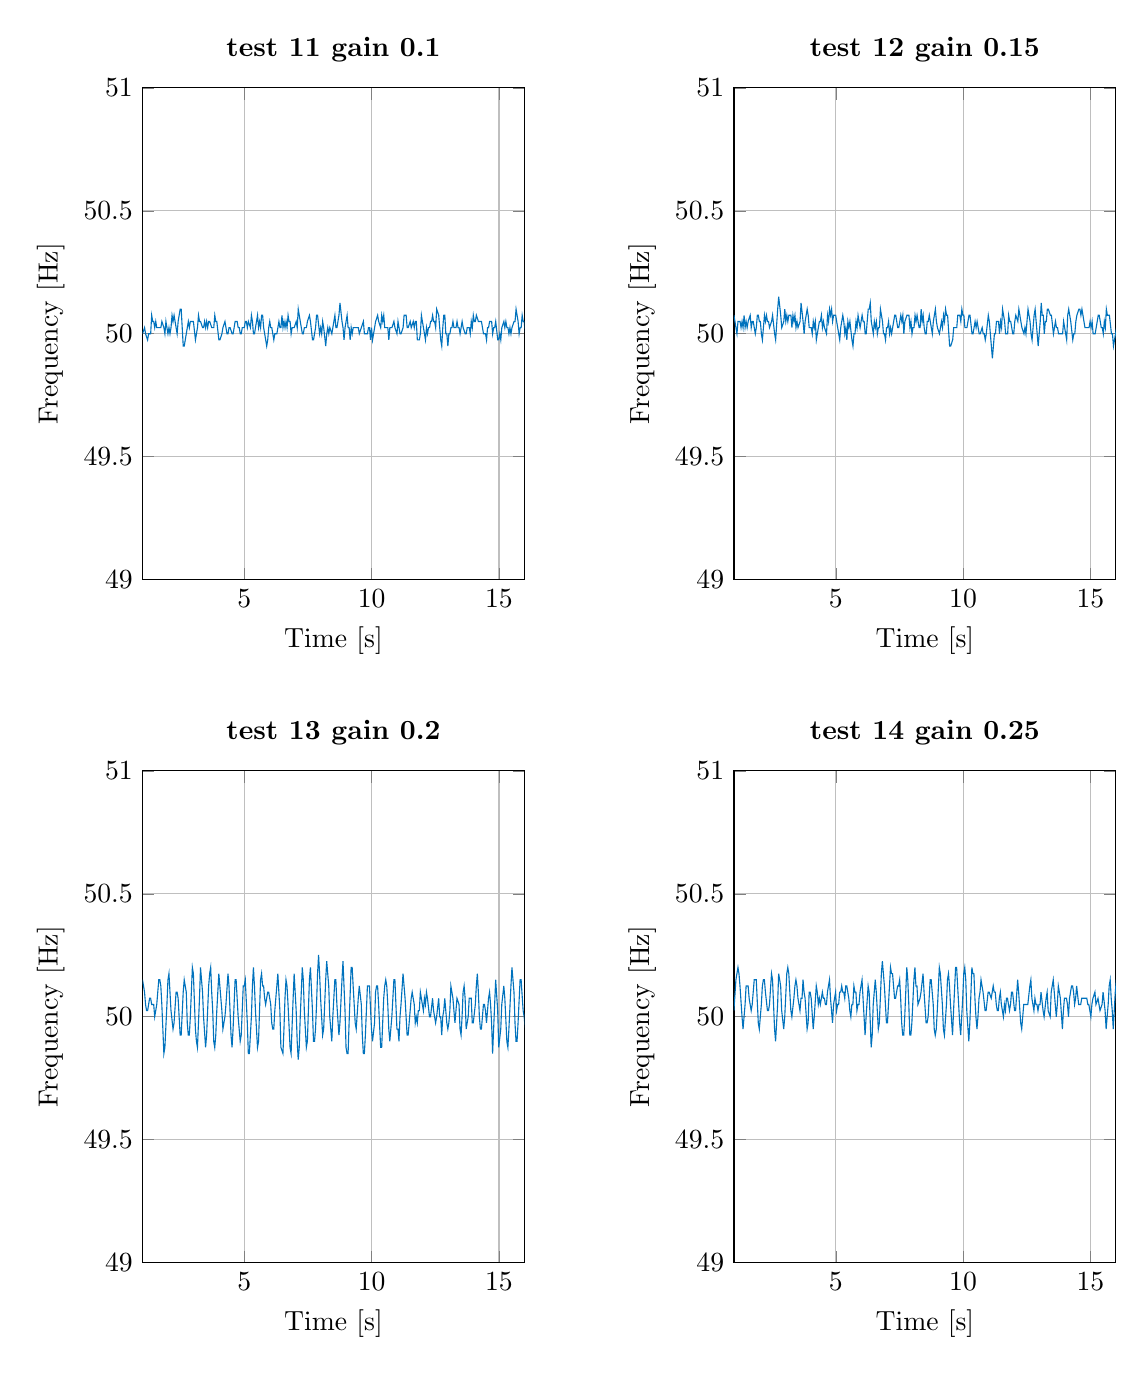
\begin{tikzpicture}

\begin{axis}[%
width=0.4\textwidth,
height=2.459in,
at={(1.043in,4.208in)},
scale only axis,
xmin=1,
xmax=16,
xlabel={Time [s]},
xmajorgrids,
ymin=49,
ymax=51,
ylabel={Frequency [Hz]},
ymajorgrids,
axis background/.style={fill=white},
title style={font=\bfseries},
title={test 11 gain 0.1}
]
\addplot [color=mycolor1,solid,forget plot]
  table[row sep=crcr]{%
0.99888	50.0000000000001\\
1.07886	50.0250125062532\\
1.11884	50\\
1.19884	49.9750124937532\\
1.23886	50\\
1.31886	50\\
1.35886	50.0751126690037\\
1.3988	50.0500500500501\\
1.43876	50.0500500500501\\
1.47872	50.025012506253\\
1.5187	50.0500500500501\\
1.55866	50.0250125062532\\
1.59864	50.025012506253\\
1.63862	50.0250125062532\\
1.6786	50.0250125062532\\
1.71858	50.025012506253\\
1.75856	50.0500500500501\\
1.83848	50.0250125062532\\
1.87846	50\\
1.91846	50.0500500500501\\
1.95842	50.0250125062532\\
1.9984	50\\
2.0384	50.0250125062532\\
2.07838	50\\
2.11838	50.0250125062532\\
2.15836	50.0751126690034\\
2.1983	50.0500500500498\\
2.23826	50.0751126690034\\
2.31816	50.0250125062532\\
2.35814	50\\
2.39814	50.0500500500498\\
2.47804	50.1002004008011\\
2.51796	50.1002004008017\\
2.59786	49.9500499500501\\
2.6379	49.9500499500496\\
2.71798	50\\
2.75798	50.0250125062532\\
2.79796	50.0500500500503\\
2.83792	50.0250125062527\\
2.8779	50.0500500500503\\
2.91786	50.0500500500498\\
2.95782	50.0500500500503\\
2.99778	50.0500500500498\\
3.07774	49.9750124937535\\
3.11776	50\\
3.15776	50.0250125062532\\
3.19774	50.0751126690034\\
3.23768	50.0500500500498\\
3.27764	50.0500500500503\\
3.35758	50.0250125062527\\
3.39756	50.0250125062532\\
3.43754	50.0500500500503\\
3.4775	50.0250125062532\\
3.51748	50.0500500500498\\
3.55744	50.0250125062532\\
3.59742	50.0500500500498\\
3.63738	50.0500500500503\\
3.7173	50.0250125062532\\
3.75728	50.0250125062532\\
3.79726	50.0250125062532\\
3.83724	50.0751126690034\\
3.87718	50.0500500500498\\
3.91714	50.0500500500503\\
3.99708	49.9750124937529\\
4.0371	49.9750124937529\\
4.11714	50\\
4.15714	50.0250125062532\\
4.2371	50.0500500500503\\
4.27706	50.0250125062532\\
4.31704	50\\
4.35704	50\\
4.39704	50.0250125062532\\
4.43702	50.0250125062532\\
4.51698	50\\
4.55698	50\\
4.63698	50.0500500500503\\
4.67694	50.0500500500492\\
4.7169	50.0500500500503\\
4.75686	50.0250125062532\\
4.79684	50.0250125062532\\
4.83682	50\\
4.87682	50\\
4.91682	50.0250125062532\\
4.99678	50.0250125062532\\
5.03676	50.0500500500492\\
5.07672	50.0500500500503\\
5.11668	50.0250125062532\\
5.15666	50.0500500500503\\
5.23658	50.0250125062521\\
5.27656	50.075112669004\\
5.3165	50.0500500500503\\
5.35646	50\\
5.39646	50\\
5.43646	50.0250125062532\\
5.5164	50.0751126690028\\
5.55634	50.0250125062532\\
5.59632	50.0500500500503\\
5.63628	50.0250125062532\\
5.67626	50.0751126690028\\
5.7162	50.075112669004\\
5.75614	50.0250125062532\\
5.79612	50\\
5.83612	49.9750124937529\\
5.87614	49.9500499500496\\
5.91618	49.975012493754\\
5.9562	50.0250125062521\\
5.99618	50.0500500500503\\
6.03614	50.0250125062532\\
6.07612	50.0250125062532\\
6.1561	49.9750124937529\\
6.19612	50\\
6.27612	50\\
6.31612	50.0250125062532\\
6.3561	50.0500500500503\\
6.39606	50.0250125062532\\
6.43604	50.0250125062532\\
6.47602	50.0751126690028\\
6.51596	50.0250125062532\\
6.55594	50.0500500500503\\
6.5959	50.0250125062532\\
6.63588	50.0500500500503\\
6.67584	50.0250125062532\\
6.71582	50.0751126690028\\
6.75576	50.0500500500503\\
6.79572	50.0500500500503\\
6.83568	50\\
6.87568	50.0250125062532\\
6.91566	50.0250125062521\\
6.95564	50.0250125062532\\
7.0356	50.0500500500503\\
7.07556	50.0250125062532\\
7.11554	50.1002004008011\\
7.15546	50.075112669004\\
7.1954	50.0500500500503\\
7.23536	50.0250125062532\\
7.27534	50\\
7.31534	50\\
7.35534	50.0250125062532\\
7.4353	50.0250125062521\\
7.47528	50.0500500500503\\
7.5552	50.075112669004\\
7.59514	50.0500500500492\\
7.67508	49.9750124937529\\
7.7151	49.975012493754\\
7.79512	50.0250125062521\\
7.8351	50.075112669004\\
7.87504	50.075112669004\\
7.95494	50\\
7.99494	50.0250125062532\\
8.03492	50.0000000000011\\
8.07492	50.0500500500492\\
8.11488	50.0250125062532\\
8.19486	49.9500499500485\\
8.2349	50.0000000000011\\
8.2749	50.0250125062532\\
8.31488	49.9999999999988\\
8.35488	50.0250125062532\\
8.43486	49.9999999999988\\
8.47486	50.0250125062532\\
8.51484	50.0500500500514\\
8.5548	50.0751126690017\\
8.59474	50.0250125062532\\
8.63472	50.0250125062532\\
8.71468	50.075112669004\\
8.75462	50.1253132832088\\
8.83442	50.0500500500514\\
8.87438	50.0250125062532\\
8.91436	49.9750124937529\\
8.95438	50.0250125062532\\
8.99436	50.0500500500492\\
9.03432	50.075112669004\\
9.07426	50.0250125062532\\
9.11424	50.0250125062532\\
9.15422	49.9750124937529\\
9.19424	50.0250125062532\\
9.23422	49.9999999999988\\
9.27422	50.0250125062532\\
9.35418	50.0250125062532\\
9.39416	50.0250125062532\\
9.47412	50.0250125062532\\
9.5141	49.9999999999988\\
9.5941	50.0250125062532\\
9.67406	50.0500500500492\\
9.71402	50.0000000000011\\
9.75402	49.9999999999988\\
9.79402	50.0000000000011\\
9.83402	49.9999999999988\\
9.87402	50.0250125062532\\
9.914	50.0250125062532\\
9.95398	49.9750124937529\\
9.994	50.0250125062532\\
10.03398	49.9750124937529\\
10.114	50.0250125062532\\
10.15398	50.0500500500492\\
10.2339	50.0751126690017\\
10.27384	50.0500500500514\\
10.35376	50.0250125062532\\
10.39374	50.075112669004\\
10.43368	50.0500500500492\\
10.47364	50.075112669004\\
10.51358	50.0250125062532\\
10.59354	50.0250125062532\\
10.63352	50.0250125062532\\
10.6735	49.9750124937529\\
10.71352	50.0250125062532\\
10.7535	50.0250125062532\\
10.79348	50.0250125062532\\
10.87344	50.0500500500492\\
10.9134	50.0250125062532\\
10.99336	50.0000000000011\\
11.03336	50.0500500500492\\
11.11328	50.0000000000011\\
11.15328	49.9999999999988\\
11.23328	50.0250125062532\\
11.27326	50.075112669004\\
11.3132	50.0751126690017\\
11.35314	50.075112669004\\
11.39308	50.0250125062532\\
11.43306	50.0250125062532\\
11.51302	50.0500500500492\\
11.55298	50.0250125062532\\
11.63294	50.0500500500514\\
11.6729	50.0250125062532\\
11.71288	50.0500500500492\\
11.75284	50.0500500500492\\
11.7928	49.9750124937551\\
11.83282	49.9750124937529\\
11.87284	49.9750124937529\\
11.91286	49.9999999999988\\
11.95286	50.075112669004\\
12.03276	50.0250125062532\\
12.07274	50.0000000000011\\
12.11274	49.9750124937529\\
12.15276	50.0250125062532\\
12.19274	49.9999999999988\\
12.23274	50.0250125062532\\
12.27272	50.0250125062532\\
12.3127	50.0500500500514\\
12.35266	50.0500500500492\\
12.39262	50.075112669004\\
12.43256	50.0500500500492\\
12.47252	50.0500500500514\\
12.51248	50.0250125062532\\
12.55246	50.1002004008011\\
12.6323	50.075112669004\\
12.67224	50.0250125062532\\
12.71222	49.9750124937529\\
12.75224	49.9500499500507\\
12.79228	50.0250125062532\\
12.83226	50.0751126690017\\
12.8722	50.075112669004\\
12.91214	50.0000000000011\\
12.95214	49.9999999999988\\
12.99214	49.9500499500507\\
13.03218	49.9999999999988\\
13.07218	50.0000000000011\\
13.11218	50.0250125062532\\
13.15216	50.0250125062532\\
13.19214	50.0500500500492\\
13.2321	50.0250125062532\\
13.27208	50.0250125062532\\
13.31206	50.0250125062532\\
13.35204	50.0500500500492\\
13.392	50.0250125062532\\
13.43198	50.0250125062532\\
13.47196	50.0000000000011\\
13.55194	50.0500500500492\\
13.5919	50.0250125062532\\
13.67188	49.9999999999988\\
13.71188	50.0000000000011\\
13.75188	50.0250125062532\\
13.79186	50.0250125062532\\
13.83184	50.025012506251\\
13.87182	50.0000000000011\\
13.91182	50.0500500500492\\
13.95178	50.0250125062532\\
13.99176	50.075112669004\\
14.0317	50.0500500500492\\
14.07166	50.0500500500514\\
14.11162	50.075112669004\\
14.1915	50.0500500500514\\
14.23146	50.0500500500492\\
14.27142	50.0500500500514\\
14.31138	50.0500500500492\\
14.35134	50.0250125062532\\
14.39132	49.9999999999988\\
14.43132	50.0000000000011\\
14.47132	49.9999999999988\\
14.51132	49.9750124937551\\
14.55134	50.0250125062532\\
14.59132	50.025012506251\\
14.6313	50.0500500500514\\
14.67126	50.0500500500492\\
14.71122	50.0500500500514\\
14.75118	49.9999999999988\\
14.79118	50.0250125062532\\
14.83116	50.0250125062532\\
14.87114	50.0500500500492\\
14.95108	49.9750124937529\\
14.9911	49.9750124937551\\
15.03112	49.9999999999988\\
15.07112	49.9750124937529\\
15.11114	50.0250125062532\\
15.19108	50.0500500500514\\
15.23104	50.0250125062532\\
15.27102	50.0500500500492\\
15.31098	50.0250125062532\\
15.35096	50.0250125062532\\
15.39094	50.0000000000011\\
15.43094	50.0250125062532\\
15.47092	49.9999999999988\\
15.51092	50.0250125062532\\
15.59088	50.0500500500492\\
15.63084	50.0500500500514\\
15.6708	50.1002004008011\\
15.71072	50.075112669004\\
15.75066	50.0500500500492\\
15.79062	50.0000000000011\\
15.83062	50.0250125062532\\
15.8706	50.0250125062532\\
15.91058	50.0751126690017\\
15.95052	50.0500500500514\\
15.99048	50.0500500500492\\
16.03044	50.0000000000011\\
};
\end{axis}

\begin{axis}[%
width=0.4\textwidth,
height=2.459in,
at={(4in,4.208in)},
scale only axis,
xmin=1,
xmax=16,
xlabel={Time [s]},
xmajorgrids,
ymin=49,
ymax=51,
ylabel={Frequency [Hz]},
ymajorgrids,
axis background/.style={fill=white},
title style={font=\bfseries},
title={test 12  gain 0.15}
]
\addplot [color=mycolor1,solid,forget plot]
  table[row sep=crcr]{%
0.99882	50.0751126690035\\
1.07874	50.025012506253\\
1.11872	50\\
1.15872	50.0500500500501\\
1.19868	50.0500500500501\\
1.23864	50.0500500500501\\
1.2786	50.0250125062532\\
1.31858	50.0500500500501\\
1.35854	50.025012506253\\
1.39852	50.0751126690037\\
1.43846	50.025012506253\\
1.47844	50.0500500500501\\
1.5184	50.0250125062532\\
1.55838	50.0500500500501\\
1.6383	50.0751126690034\\
1.67824	50.0250125062532\\
1.71822	50.0500500500501\\
1.75818	50.0500500500501\\
1.83812	50\\
1.87812	50.025012506253\\
1.9181	50.0751126690037\\
1.95804	50.0751126690034\\
1.99798	50.0500500500501\\
2.03794	50.0500500500503\\
2.0779	50\\
2.1179	49.9750124937529\\
2.19792	50.0751126690034\\
2.23786	50.0500500500503\\
2.27782	50.0751126690034\\
2.31776	50.0500500500503\\
2.35772	50.0500500500498\\
2.39768	50.0250125062532\\
2.47762	50.0500500500503\\
2.51758	50.0751126690034\\
2.59748	50\\
2.63748	49.9750124937529\\
2.71748	50.1002004008017\\
2.7574	50.150451354062\\
2.8372	50.0751126690034\\
2.87714	50.0250125062532\\
2.9571	50.0500500500498\\
2.99706	50.1002004008017\\
3.03698	50.0500500500503\\
3.07694	50.0751126690034\\
3.11688	50.0500500500498\\
3.15684	50.075112669004\\
3.19678	50.0751126690034\\
3.23672	50.0751126690034\\
3.27666	50.0250125062532\\
3.31664	50.0751126690034\\
3.35658	50.0500500500498\\
3.39654	50.075112669004\\
3.43648	50.0250125062527\\
3.47646	50.0500500500503\\
3.51642	50.0250125062532\\
3.59636	50.0500500500503\\
3.63632	50.1253132832077\\
3.71614	50.0500500500503\\
3.7561	50\\
3.7961	50.0500500500498\\
3.876	50.1002004008011\\
3.91592	50.075112669004\\
3.95586	50.0250125062527\\
3.99584	50.0250125062538\\
4.03582	50.0250125062532\\
4.0758	50\\
4.1158	50.0500500500492\\
4.15576	50.0250125062532\\
4.19574	50.0500500500503\\
4.2357	49.9750124937529\\
4.27572	50\\
4.3557	50.0500500500503\\
4.39566	50.0500500500503\\
4.43562	50.0751126690028\\
4.47556	50.0250125062532\\
4.51554	50.0500500500503\\
4.5555	50.0250125062532\\
4.63546	50\\
4.67546	50.0751126690028\\
4.7154	50.0500500500503\\
4.75536	50.1002004008011\\
4.79528	50.075112669004\\
4.83522	50.1002004008022\\
4.87514	50.0500500500492\\
4.9151	50.075112669004\\
4.95504	50.0751126690028\\
4.99498	50.075112669004\\
5.03492	50.0500500500503\\
5.11486	50\\
5.15486	49.9750124937529\\
5.19488	50.0250125062532\\
5.2748	50.075112669004\\
5.31474	50.0500500500503\\
5.3547	50\\
5.3947	50.0250125062532\\
5.43468	49.9750124937529\\
5.4747	50.0500500500503\\
5.51466	50.0250125062532\\
5.55464	50.0500500500492\\
5.63462	49.9750124937529\\
5.67464	49.9500499500496\\
5.71468	50\\
5.75468	50\\
5.79468	50.0500500500503\\
5.83464	50.0250125062532\\
5.87462	50.0751126690028\\
5.91456	50.0500500500503\\
5.95452	50.0250125062532\\
6.03448	50.075112669004\\
6.07442	50.0500500500492\\
6.11438	50.0500500500503\\
6.15434	50\\
6.19434	50\\
6.27434	50.1002004008022\\
6.31426	50.1002004008011\\
6.35418	50.1253132832077\\
6.39408	50.0500500500503\\
6.43404	50.0250125062532\\
6.47402	50\\
6.51402	50.0500500500503\\
6.55398	50.0250125062532\\
6.59396	50.0500500500492\\
6.63392	50\\
6.67392	50.0250125062532\\
6.7139	50.0250125062532\\
6.75388	50.1002004008022\\
6.7938	50.0751126690028\\
6.83374	50.0500500500503\\
6.8737	50\\
6.9137	50\\
6.9537	49.9750124937529\\
6.99372	50.0250125062532\\
7.0337	50.0250125062532\\
7.07368	50.0500500500503\\
7.11364	50\\
7.15364	50.0250125062532\\
7.19362	50\\
7.23362	50.0250125062532\\
7.31356	50.0751126690028\\
7.3535	50.075112669004\\
7.43338	50.0250125062532\\
7.47336	50.0250125062532\\
7.5533	50.0751126690028\\
7.59324	50.0500500500503\\
7.6332	50.075112669004\\
7.67314	50\\
7.71314	50.0500500500503\\
7.79304	50.075112669004\\
7.83298	50.0751126690028\\
7.87292	50.075112669004\\
7.91286	50.0250125062532\\
7.95284	50.0500500500503\\
7.9928	49.9999999999988\\
8.0328	50.0250125062532\\
8.07278	50.0250125062532\\
8.11276	50.075112669004\\
8.1527	50.0500500500492\\
8.19266	50.075112669004\\
8.2326	50.0500500500514\\
8.27256	50.0250125062532\\
8.31254	50.0250125062532\\
8.35252	50.1002004008011\\
8.39244	50.0500500500492\\
8.4324	50.075112669004\\
8.47234	50.0250125062532\\
8.51232	49.9999999999988\\
8.55232	50.0000000000011\\
8.59232	50.0500500500492\\
8.63228	50.0500500500514\\
8.67224	50.0751126690017\\
8.71218	50.0500500500514\\
8.75214	50.0250125062532\\
8.79212	49.9999999999988\\
8.83212	50.0500500500514\\
8.87208	50.0751126690017\\
8.91202	50.1002004008033\\
8.95194	50.0500500500492\\
8.9919	50.0250125062532\\
9.07188	49.9999999999988\\
9.11188	50.0250125062532\\
9.15186	50.0500500500492\\
9.19182	50.0250125062532\\
9.2318	50.075112669004\\
9.27174	50.0500500500514\\
9.3117	50.1002004008011\\
9.35162	50.075112669004\\
9.39156	50.0751126690017\\
9.4715	49.9500499500507\\
9.51154	49.9500499500485\\
9.59162	49.9750124937529\\
9.63164	50.0250125062532\\
9.7116	50.0250125062532\\
9.75158	50.0250125062532\\
9.79156	50.075112669004\\
9.8315	50.0751126690017\\
9.87144	50.075112669004\\
9.91138	50.0500500500514\\
9.95134	50.1002004008011\\
9.99126	50.075112669004\\
10.0312	50.0751126690017\\
10.07114	50.0250125062532\\
10.11112	50.0250125062532\\
10.1511	50.0250125062532\\
10.23104	50.0751126690017\\
10.27098	50.075112669004\\
10.3509	50.0000000000011\\
10.3909	49.9999999999988\\
10.4709	50.0500500500492\\
10.51086	50.0250125062532\\
10.55084	50.0500500500492\\
10.5908	50.0250125062532\\
10.63078	50.0000000000011\\
10.67078	49.9999999999988\\
10.75078	50.0250125062532\\
10.79076	49.9999999999988\\
10.83076	50.0000000000011\\
10.87076	49.9750124937529\\
10.91078	50.0000000000011\\
10.99076	50.075112669004\\
11.0307	50.0500500500514\\
11.11064	49.9500499500485\\
11.15068	49.9001996007988\\
11.23084	49.9999999999988\\
11.27084	50.0000000000011\\
11.31084	50.0500500500492\\
11.3508	50.0500500500514\\
11.39076	50.0500500500492\\
11.43072	50.0000000000011\\
11.47072	50.0500500500492\\
11.51068	50.0250125062532\\
11.55066	50.1002004008011\\
11.63052	50.0500500500492\\
11.67048	50.0000000000011\\
11.71048	49.9999999999988\\
11.75048	50.0000000000011\\
11.79048	50.075112669004\\
11.83042	50.0500500500492\\
11.87038	50.0500500500492\\
11.91034	50.0250125062532\\
11.95032	50.0000000000011\\
11.99032	49.9999999999988\\
12.03032	50.0500500500514\\
12.07028	50.075112669004\\
12.15016	50.0500500500514\\
12.19012	50.1002004008011\\
12.26998	50.0500500500492\\
12.30994	50.0250125062532\\
12.3899	50.0000000000011\\
12.4299	50.0250125062532\\
12.46988	49.9999999999988\\
12.50988	50.0500500500492\\
12.54984	50.1002004008033\\
12.6297	50.0500500500514\\
12.66966	49.9999999999988\\
12.70966	49.9750124937529\\
12.78964	50.075112669004\\
12.82958	50.1002004008011\\
12.90948	49.9999999999988\\
12.94948	49.9500499500507\\
13.02952	50.0500500500492\\
13.06948	50.1253132832088\\
13.10938	50.0751126690017\\
13.14932	50.075112669004\\
13.18926	50.0000000000011\\
13.22926	50.0500500500492\\
13.26922	50.0500500500492\\
13.30918	50.1002004008033\\
13.3491	50.1002004008011\\
13.42894	50.075112669004\\
13.46888	50.075112669004\\
13.54878	50.0000000000011\\
13.58878	50.0250125062532\\
13.62876	50.0500500500492\\
13.66872	50.0250125062532\\
13.7087	50.0250125062532\\
13.74868	49.9999999999988\\
13.78868	50.0000000000011\\
13.82868	49.9999999999988\\
13.86868	50.0000000000011\\
13.90868	49.9999999999988\\
13.94868	50.0500500500514\\
13.98864	50.0250125062532\\
14.0686	49.9750124937529\\
14.10862	50.075112669004\\
14.14856	50.1002004008011\\
14.18848	50.075112669004\\
14.22842	50.0500500500492\\
14.30836	49.9750124937529\\
14.34838	50.0000000000011\\
14.38838	49.9999999999988\\
14.42838	50.0500500500492\\
14.46834	50.075112669004\\
14.5482	50.1002004008033\\
14.58812	50.1002004008011\\
14.62804	50.075112669004\\
14.66798	50.1002004008011\\
14.7079	50.075112669004\\
14.74784	50.0500500500492\\
14.7878	50.0250125062532\\
14.82778	50.0250125062532\\
14.86776	50.0250125062532\\
14.94772	50.0250125062532\\
14.9877	50.0500500500492\\
15.02766	50.0250125062532\\
15.06764	50.0500500500514\\
15.1076	49.9999999999988\\
15.1476	50.0000000000011\\
15.1876	49.9999999999988\\
15.2276	50.0250125062532\\
15.30754	50.075112669004\\
15.34748	50.075112669004\\
15.38742	50.0500500500492\\
15.42738	50.0250125062532\\
15.46736	50.0250125062532\\
15.50734	50.0000000000011\\
15.54734	50.0500500500492\\
15.5873	50.0250125062532\\
15.62728	50.1002004008011\\
15.6672	50.075112669004\\
15.70714	50.075112669004\\
15.74708	50.075112669004\\
15.82698	50.0000000000011\\
15.86698	49.9999999999988\\
15.90698	49.9500499500507\\
15.94702	49.9750124937529\\
15.98704	49.9999999999988\\
16.02704	50.0250125062532\\
};
\end{axis}

\begin{axis}[%
width=0.4\textwidth,
height=2.459in,
at={(1.043in,0.793in)},
scale only axis,
xmin=1,
xmax=16,
xlabel={Time [s]},
xmajorgrids,
ymin=49,
ymax=51,
ylabel={Frequency [Hz]},
ymajorgrids,
axis background/.style={fill=white},
title style={font=\bfseries},
title={test 13  gain 0.2}
]
\addplot [color=mycolor1,solid,forget plot]
  table[row sep=crcr]{%
0.99842	50.150451354062\\
1.0782	50.1002004008014\\
1.11812	50.0500500500501\\
1.15808	50.0250125062532\\
1.19806	50.0250125062532\\
1.23804	50.0500500500501\\
1.278	50.0751126690034\\
1.31794	50.0751126690034\\
1.35788	50.0500500500501\\
1.4378	50.0500500500501\\
1.47776	50.0000000000002\\
1.55774	50.0500500500501\\
1.5977	50.1002004008017\\
1.63762	50.1504513540623\\
1.6775	50.150451354062\\
1.71738	50.125313283208\\
1.75728	50.0500500500501\\
1.8373	49.850448654038\\
1.87742	49.8753117206982\\
1.95758	50.0500500500501\\
1.99754	50.150451354062\\
2.03742	50.1756146512795\\
2.07728	50.1002004008017\\
2.1172	50.0250125062532\\
2.1972	49.9500499500496\\
2.23724	49.9750124937535\\
2.31722	50.1002004008017\\
2.35714	50.1002004008017\\
2.39706	50.0751126690034\\
2.47702	49.9251123315028\\
2.51708	49.9251123315028\\
2.59714	50.1002004008011\\
2.63706	50.1504513540626\\
2.71682	50.1002004008017\\
2.75674	49.9750124937529\\
2.79676	49.9251123315028\\
2.83682	49.9251123315028\\
2.87688	50\\
2.95682	50.200803212851\\
2.99666	50.1756146512795\\
3.07644	49.9500499500501\\
3.11648	49.9001996007983\\
3.15656	49.8753117206985\\
3.23668	50.0751126690034\\
3.27662	50.2008032128516\\
3.3563	50.1002004008017\\
3.39622	50\\
3.47628	49.875311720698\\
3.51638	49.9251123315028\\
3.5964	50.1253132832077\\
3.6363	50.1756146512795\\
3.67616	50.2008032128516\\
3.716	50.1002004008017\\
3.75592	50.0250125062532\\
3.7959	49.9001996007983\\
3.83598	49.8753117206985\\
3.87608	49.9251123315028\\
3.91614	50.0250125062527\\
3.99604	50.1756146512795\\
4.0359	50.1253132832088\\
4.11572	50.0250125062532\\
4.1557	49.9500499500496\\
4.23578	50\\
4.27578	50.0500500500492\\
4.35562	50.1756146512795\\
4.39548	50.1253132832088\\
4.47538	49.9251123315022\\
4.51544	49.8753117206985\\
4.55554	49.9500499500496\\
4.63556	50.1504513540631\\
4.67544	50.150451354062\\
4.75524	50\\
4.79524	49.9500499500507\\
4.83528	49.9001996007977\\
4.87536	49.9251123315033\\
4.91542	50.0250125062532\\
4.9554	50.1253132832077\\
4.9953	50.1253132832077\\
5.0352	50.150451354062\\
5.11502	49.9750124937529\\
5.15504	49.850448654038\\
5.19516	49.850448654038\\
5.27536	50\\
5.31536	50.1253132832077\\
5.35526	50.2008032128516\\
5.3951	50.1253132832077\\
5.435	50.0250125062532\\
5.51506	49.8753117206974\\
5.55516	49.9001996007988\\
5.63522	50.150451354062\\
5.6751	50.1756146512795\\
5.71496	50.1253132832077\\
5.75486	50.1253132832088\\
5.79476	50.0751126690028\\
5.8347	50.0500500500503\\
5.9146	50.1002004008011\\
5.95452	50.1002004008022\\
6.03436	50.0500500500503\\
6.07432	49.9750124937529\\
6.11434	49.9500499500496\\
6.15438	49.9500499500507\\
6.19442	50.0250125062532\\
6.27434	50.1253132832077\\
6.31424	50.1756146512795\\
6.39402	50.0250125062532\\
6.434	49.8753117206985\\
6.5142	49.850448654038\\
6.55432	49.9500499500507\\
6.59436	50.0751126690028\\
6.6343	50.150451354062\\
6.67418	50.1253132832088\\
6.71408	50.0500500500492\\
6.79412	49.8753117206985\\
6.83422	49.850448654038\\
6.91438	50.075112669004\\
6.95432	50.1756146512795\\
7.03406	50.0250125062532\\
7.07404	49.9001996007977\\
7.11412	49.825610363728\\
7.15426	49.8753117206974\\
7.19436	50\\
7.23436	50.1002004008022\\
7.27428	50.2008032128516\\
7.31412	50.150451354062\\
7.354	50.0250125062532\\
7.43406	49.8753117206985\\
7.47416	49.9001996007988\\
7.55422	50.150451354062\\
7.5941	50.2008032128516\\
7.67384	50.0250125062532\\
7.71382	49.9001996007988\\
7.7539	49.9001996007977\\
7.79398	49.9500499500507\\
7.83402	50.0500500500492\\
7.87398	50.1756146512795\\
7.91384	50.2512562814075\\
7.95364	50.1756146512795\\
7.9935	50.075112669004\\
8.07348	49.9251123315044\\
8.11354	49.9500499500485\\
8.19354	50.150451354062\\
8.23342	50.226017076845\\
8.3131	50.1253132832066\\
8.353	50.0000000000011\\
8.43306	49.9001996007988\\
8.47314	49.9999999999988\\
8.55308	50.150451354062\\
8.59296	50.150451354062\\
8.63284	50.0500500500514\\
8.71284	49.9251123315044\\
8.7529	49.9750124937529\\
8.83288	50.150451354062\\
8.87276	50.2260170768472\\
8.95248	50.0250125062532\\
8.99246	49.8753117206996\\
9.03256	49.8504486540358\\
9.07268	49.850448654038\\
9.1128	49.9750124937551\\
9.19274	50.2008032128516\\
9.23258	50.2008032128516\\
9.27242	50.1253132832066\\
9.3523	49.9750124937529\\
9.39232	49.9500499500507\\
9.47236	50.0751126690017\\
9.5123	50.1253132832088\\
9.5921	50.0500500500492\\
9.63206	49.9251123315022\\
9.67212	49.850448654038\\
9.71224	49.850448654038\\
9.75236	49.9251123315022\\
9.8324	50.1253132832088\\
9.8723	50.1253132832088\\
9.9122	50.1253132832066\\
9.99208	49.9500499500507\\
10.03212	49.9001996007988\\
10.11226	49.9750124937529\\
10.15228	50.1002004008011\\
10.1922	50.1253132832088\\
10.2321	50.1253132832088\\
10.272	50.0500500500492\\
10.352	49.8753117206974\\
10.3921	49.8753117206974\\
10.47224	50.075112669004\\
10.51218	50.1253132832088\\
10.55208	50.150451354062\\
10.59196	50.1253132832066\\
10.63186	50.0500500500514\\
10.67182	49.9500499500485\\
10.71186	49.9001996007988\\
10.75194	49.9500499500507\\
10.79198	49.9999999999988\\
10.87188	50.150451354062\\
10.91176	50.150451354062\\
10.99158	49.9500499500507\\
11.03162	49.9500499500485\\
11.07166	49.9001996007988\\
11.11174	50.0000000000011\\
11.15174	50.0500500500492\\
11.23158	50.1756146512806\\
11.27144	50.1253132832066\\
11.31134	50.075112669004\\
11.39128	49.9251123315022\\
11.43134	49.9251123315022\\
11.51142	50.0250125062532\\
11.5514	50.075112669004\\
11.59134	50.1002004008011\\
11.63126	50.075112669004\\
11.6712	50.0500500500492\\
11.71116	49.9750124937529\\
11.75118	50.0000000000011\\
11.79118	49.9750124937529\\
11.8312	50.0250125062532\\
11.87118	50.0250125062532\\
11.91116	50.1002004008011\\
11.95108	50.075112669004\\
12.03098	50.0250125062532\\
12.07096	50.075112669004\\
12.1109	50.0500500500492\\
12.15086	50.1002004008033\\
12.19078	50.0751126690017\\
12.2707	50.0000000000011\\
12.3107	49.9999999999988\\
12.39068	50.075112669004\\
12.43062	50.0250125062532\\
12.51058	49.9750124937529\\
12.5506	50.0000000000011\\
12.63058	50.075112669004\\
12.67052	49.9999999999988\\
12.71052	50.0000000000011\\
12.75052	49.9251123315022\\
12.79058	49.9999999999988\\
12.83058	50.0250125062532\\
12.87056	50.075112669004\\
12.9105	50.0250125062532\\
12.95048	49.9750124937529\\
12.9905	49.9500499500507\\
13.03054	49.9750124937529\\
13.07056	50.0250125062532\\
13.11054	50.1253132832066\\
13.15044	50.1002004008033\\
13.19036	50.0751126690017\\
13.27032	49.9750124937529\\
13.31034	50.0250125062532\\
13.35032	50.0751126690017\\
13.43022	50.0500500500492\\
13.47018	49.9500499500507\\
13.51022	49.9251123315022\\
13.55028	50.0000000000011\\
13.59028	50.1002004008011\\
13.6302	50.1253132832088\\
13.6701	50.0751126690017\\
13.71004	49.9500499500507\\
13.7901	50.0000000000011\\
13.8301	50.0751126690017\\
13.87004	50.075112669004\\
13.90998	50.075112669004\\
13.94992	49.9750124937529\\
13.98994	49.9750124937529\\
14.06998	50.0500500500514\\
14.10994	50.1253132832066\\
14.14984	50.1756146512806\\
14.1897	50.1002004008011\\
14.22962	50.0000000000011\\
14.26962	49.9500499500485\\
14.30966	49.9500499500507\\
14.3497	49.9999999999988\\
14.3897	50.0500500500514\\
14.42966	50.0500500500492\\
14.46962	50.0250125062532\\
14.5096	49.9750124937529\\
14.54962	50.0250125062532\\
14.5896	50.075112669004\\
14.62954	50.1002004008011\\
14.66946	50.0500500500514\\
14.70942	49.9750124937529\\
14.74944	49.850448654038\\
14.8296	50.0500500500514\\
14.86956	50.150451354062\\
14.94936	50.0250125062532\\
14.98934	49.8753117206974\\
15.06954	49.9500499500485\\
15.10958	50.0500500500514\\
15.18946	50.1253132832088\\
15.22936	50.0751126690017\\
15.30932	49.9001996007966\\
15.3494	49.8753117206996\\
15.3895	49.9500499500485\\
15.46952	50.1253132832088\\
15.50942	50.2008032128516\\
15.58914	50.1002004008011\\
15.62906	49.9750124937529\\
15.66908	49.9001996007988\\
15.70916	49.9001996007988\\
15.74924	49.9750124937529\\
15.82922	50.1504513540642\\
15.8691	50.150451354062\\
15.94888	50.0250125062532\\
15.98886	50.0000000000011\\
16.02886	49.9500499500485\\
};
\end{axis}

\begin{axis}[%
width=0.4\textwidth,
height=2.459in,
at={(4in,0.793in)},
scale only axis,
xmin=1,
xmax=16,
xlabel={Time [s]},
xmajorgrids,
ymin=49,
ymax=51,
ylabel={Frequency [Hz]},
ymajorgrids,
axis background/.style={fill=white},
title style={font=\bfseries},
title={test 14  gain 0.25}
]
\addplot [color=mycolor1,solid,forget plot]
  table[row sep=crcr]{%
0.9981	50.0250125062531\\
1.07802	50.1504513540623\\
1.1179	50.1756146512795\\
1.15776	50.2008032128513\\
1.1976	50.1756146512798\\
1.23746	50.125313283208\\
1.3173	50\\
1.3573	49.9500499500501\\
1.43734	50.0500500500501\\
1.4773	50.125313283208\\
1.5571	50.1253132832082\\
1.597	50.0751126690034\\
1.6769	50.0250125062532\\
1.71688	50.0500500500501\\
1.75684	50.1002004008014\\
1.79676	50.1504513540623\\
1.83664	50.1504513540623\\
1.87652	50.150451354062\\
1.95634	49.9750124937529\\
1.99636	49.9500499500499\\
2.0764	50.0500500500503\\
2.11636	50.1253132832082\\
2.15626	50.150451354062\\
2.19614	50.150451354062\\
2.23602	50.1002004008017\\
2.3159	50.0250125062527\\
2.35588	50.0250125062532\\
2.39586	50.0500500500503\\
2.4757	50.1756146512795\\
2.51556	50.150451354062\\
2.59538	49.9500499500496\\
2.63542	49.9001996007988\\
2.71554	50.0500500500503\\
2.7555	50.1756146512795\\
2.83522	50.1253132832077\\
2.87512	50.0250125062532\\
2.95514	49.9500499500496\\
2.99518	50.0000000000005\\
3.0751	50.17561465128\\
3.11496	50.200803212851\\
3.1548	50.1756146512795\\
3.23458	50.0250125062532\\
3.27456	50\\
3.35456	50.0751126690034\\
3.3945	50.1253132832082\\
3.4344	50.150451354062\\
3.47428	50.1253132832082\\
3.51418	50.0751126690034\\
3.59408	50.0250125062527\\
3.63406	50.075112669004\\
3.674	50.0751126690034\\
3.71394	50.150451354062\\
3.75382	50.1002004008017\\
3.79374	50.0751126690034\\
3.8737	49.9500499500496\\
3.91374	49.9750124937535\\
3.95376	50.1002004008017\\
3.99368	50.1002004008011\\
4.0336	50.075112669004\\
4.11356	49.9500499500496\\
4.1536	50\\
4.23354	50.1253132832077\\
4.27344	50.1002004008022\\
4.31336	50.0500500500503\\
4.35332	50.0751126690028\\
4.39326	50.0500500500503\\
4.43322	50.0751126690028\\
4.47316	50.1002004008022\\
4.51308	50.075112669004\\
4.55302	50.0751126690028\\
4.59296	50.0500500500503\\
4.63292	50.0500500500503\\
4.67288	50.1002004008011\\
4.7527	50.1504513540631\\
4.79258	50.0751126690028\\
4.8725	49.9750124937529\\
4.91252	50.0500500500503\\
4.9924	50.1002004008022\\
5.03232	50.0250125062532\\
5.0723	50.0500500500503\\
5.11226	50.0500500500492\\
5.15222	50.1002004008022\\
5.19214	50.1002004008011\\
5.23206	50.1253132832077\\
5.27196	50.1002004008022\\
5.31188	50.1002004008011\\
5.3518	50.075112669004\\
5.39174	50.1253132832077\\
5.43164	50.1253132832088\\
5.51144	50.075112669004\\
5.55138	50.0250125062521\\
5.59136	50\\
5.63136	50.0500500500503\\
5.67132	50.0500500500503\\
5.71128	50.1253132832077\\
5.75118	50.1002004008022\\
5.7911	50.1002004008011\\
5.83102	50.0250125062532\\
5.871	50.0500500500503\\
5.91096	50.0500500500503\\
5.95092	50.1002004008011\\
6.03076	50.1504513540631\\
6.07064	50.0751126690028\\
6.15058	49.9251123315033\\
6.19064	50\\
6.27056	50.1253132832088\\
6.31046	50.1002004008011\\
6.3904	49.8753117206985\\
6.4305	49.9251123315022\\
6.47056	50.0500500500503\\
6.5504	50.1504513540631\\
6.59028	50.1002004008011\\
6.6702	49.9500499500496\\
6.71024	49.975012493754\\
6.79018	50.1756146512795\\
6.83004	50.2260170768461\\
6.9097	50.1253132832077\\
6.9496	50.0500500500503\\
6.98956	49.9750124937529\\
7.02958	49.9750124937529\\
7.0696	50.0500500500503\\
7.14948	50.2008032128516\\
7.18932	50.1756146512795\\
7.22918	50.1756146512795\\
7.30894	50.075112669004\\
7.34888	50.075112669004\\
7.42874	50.1253132832077\\
7.46864	50.1253132832088\\
7.50854	50.150451354062\\
7.54842	50.0751126690028\\
7.58836	49.975012493754\\
7.62838	49.9251123315022\\
7.66844	49.9251123315033\\
7.7085	50\\
7.78842	50.2008032128516\\
7.82826	50.150451354062\\
7.86814	50.0500500500503\\
7.9081	49.9251123315022\\
7.94816	49.9251123315033\\
7.98822	49.975012493754\\
8.06818	50.150451354062\\
8.10806	50.2008032128516\\
8.1479	50.1253132832088\\
8.1878	50.1253132832088\\
8.2277	50.0500500500492\\
8.30762	50.075112669004\\
8.34756	50.1002004008011\\
8.42738	50.1756146512806\\
8.46724	50.1002004008011\\
8.54712	49.9750124937529\\
8.58714	49.9750124937529\\
8.62716	50.0000000000011\\
8.7071	50.150451354062\\
8.74698	50.150451354062\\
8.82678	50.0500500500492\\
8.86674	49.9500499500507\\
8.90678	49.9251123315022\\
8.94684	49.9500499500507\\
8.98688	50.0250125062532\\
9.06676	50.2008032128516\\
9.1066	50.1756146512784\\
9.18634	50.0500500500514\\
9.2263	49.9500499500485\\
9.26634	49.9251123315022\\
9.34644	50.0500500500514\\
9.3864	50.150451354062\\
9.42628	50.1756146512784\\
9.46614	50.1253132832088\\
9.50604	50.0500500500492\\
9.58602	49.9251123315022\\
9.62608	50.0250125062532\\
9.706	50.2008032128516\\
9.74584	50.2008032128516\\
9.82558	50.0500500500492\\
9.86554	49.9750124937529\\
9.90556	49.9251123315022\\
9.98564	50.0751126690017\\
10.02558	50.1756146512806\\
10.06544	50.2008032128516\\
10.10528	50.150451354062\\
10.14516	50.0250125062532\\
10.2252	49.9001996007988\\
10.26528	49.9750124937529\\
10.34524	50.2008032128516\\
10.38508	50.1756146512784\\
10.42494	50.1756146512806\\
10.4648	50.0751126690017\\
10.50474	50.0000000000011\\
10.54474	49.9500499500507\\
10.58478	49.9999999999988\\
10.62478	50.075112669004\\
10.66472	50.1002004008011\\
10.70464	50.150451354062\\
10.74452	50.1253132832088\\
10.78442	50.1002004008011\\
10.86428	50.0250125062532\\
10.90426	50.0250125062532\\
10.9842	50.1002004008011\\
11.02412	50.1002004008033\\
11.10398	50.0751126690017\\
11.14392	50.1002004008033\\
11.18384	50.1253132832066\\
11.22374	50.1002004008011\\
11.26366	50.1002004008033\\
11.30358	50.0500500500492\\
11.34354	50.0250125062532\\
11.38352	50.0250125062532\\
11.4235	50.075112669004\\
11.46344	50.1002004008011\\
11.50336	50.0500500500492\\
11.54332	50.0250125062532\\
11.5833	50.0000000000011\\
11.6233	50.0500500500492\\
11.66326	50.0250125062532\\
11.70324	50.075112669004\\
11.74318	50.075112669004\\
11.78312	50.0500500500492\\
11.82308	50.0250125062532\\
11.86306	50.0500500500492\\
11.90302	50.1002004008033\\
11.94294	50.1002004008011\\
12.02282	50.0250125062532\\
12.0628	50.0250125062532\\
12.1427	50.150451354062\\
12.18258	50.1002004008033\\
12.26248	49.9750124937529\\
12.3025	49.9500499500485\\
12.38252	50.0500500500514\\
12.42248	50.0500500500492\\
12.5024	50.0500500500514\\
12.54236	50.0500500500492\\
12.62226	50.1253132832088\\
12.66216	50.150451354062\\
12.70204	50.075112669004\\
12.78194	50.0250125062532\\
12.82192	50.075112669004\\
12.86186	50.0500500500492\\
12.90182	50.0500500500492\\
12.94178	50.0250125062532\\
12.98176	50.0500500500514\\
13.02172	50.0500500500492\\
13.06168	50.1002004008011\\
13.14156	50.0250125062532\\
13.18154	49.9999999999988\\
13.26152	50.075112669004\\
13.30146	50.1002004008011\\
13.34138	50.0250125062532\\
13.42134	50.0000000000011\\
13.46134	50.1002004008011\\
13.54116	50.1504513540642\\
13.58104	50.1002004008011\\
13.66094	49.9999999999988\\
13.70094	50.0500500500514\\
13.7409	50.1253132832066\\
13.7808	50.1002004008011\\
13.82072	50.075112669004\\
13.90064	49.9500499500507\\
13.94068	50.0250125062532\\
13.98066	50.075112669004\\
14.0206	50.0751126690017\\
14.06054	50.075112669004\\
14.10048	50.0500500500514\\
14.14044	49.9999999999988\\
14.18044	50.075112669004\\
14.22038	50.1002004008011\\
14.2603	50.1253132832088\\
14.3002	50.1253132832066\\
14.3401	50.1002004008033\\
14.38002	50.0500500500492\\
14.41998	50.075112669004\\
14.45992	50.1253132832088\\
14.53974	50.0500500500492\\
14.5797	50.0500500500514\\
14.61966	50.0500500500492\\
14.65962	50.075112669004\\
14.69956	50.075112669004\\
14.7395	50.0751126690017\\
14.77944	50.075112669004\\
14.81938	50.075112669004\\
14.85932	50.075112669004\\
14.89926	50.0500500500492\\
14.93922	50.0500500500492\\
14.97918	50.0250125062532\\
15.01916	50.0000000000011\\
15.05916	50.0500500500492\\
15.09912	50.075112669004\\
15.17898	50.1002004008033\\
15.2189	50.0500500500492\\
15.29882	50.075112669004\\
15.33876	50.0500500500492\\
15.37872	50.0250125062532\\
15.45868	50.0500500500514\\
15.49864	50.1002004008011\\
15.57848	50.0250125062532\\
15.61846	49.9500499500507\\
15.69852	50.0500500500492\\
15.73848	50.1253132832088\\
15.77838	50.150451354062\\
15.81826	50.075112669004\\
15.8582	50.0250125062532\\
15.89818	49.9500499500485\\
15.93822	50.0250125062532\\
15.9782	50.1002004008011\\
16.01812	50.150451354062\\
};
\end{axis}
\end{tikzpicture}%
\caption{Steady state at 10 kW load, with various scaling factors.}
\label{fig:test11-14steadyfrequency10kw}
\end{figure}

\begin{figure}[H]
\centering
% This file was created by matlab2tikz.
%
%The latest updates can be retrieved from
%  http://www.mathworks.com/matlabcentral/fileexchange/22022-matlab2tikz-matlab2tikz
%where you can also make suggestions and rate matlab2tikz.
%
\definecolor{mycolor1}{rgb}{0.00000,0.44700,0.74100}%
%
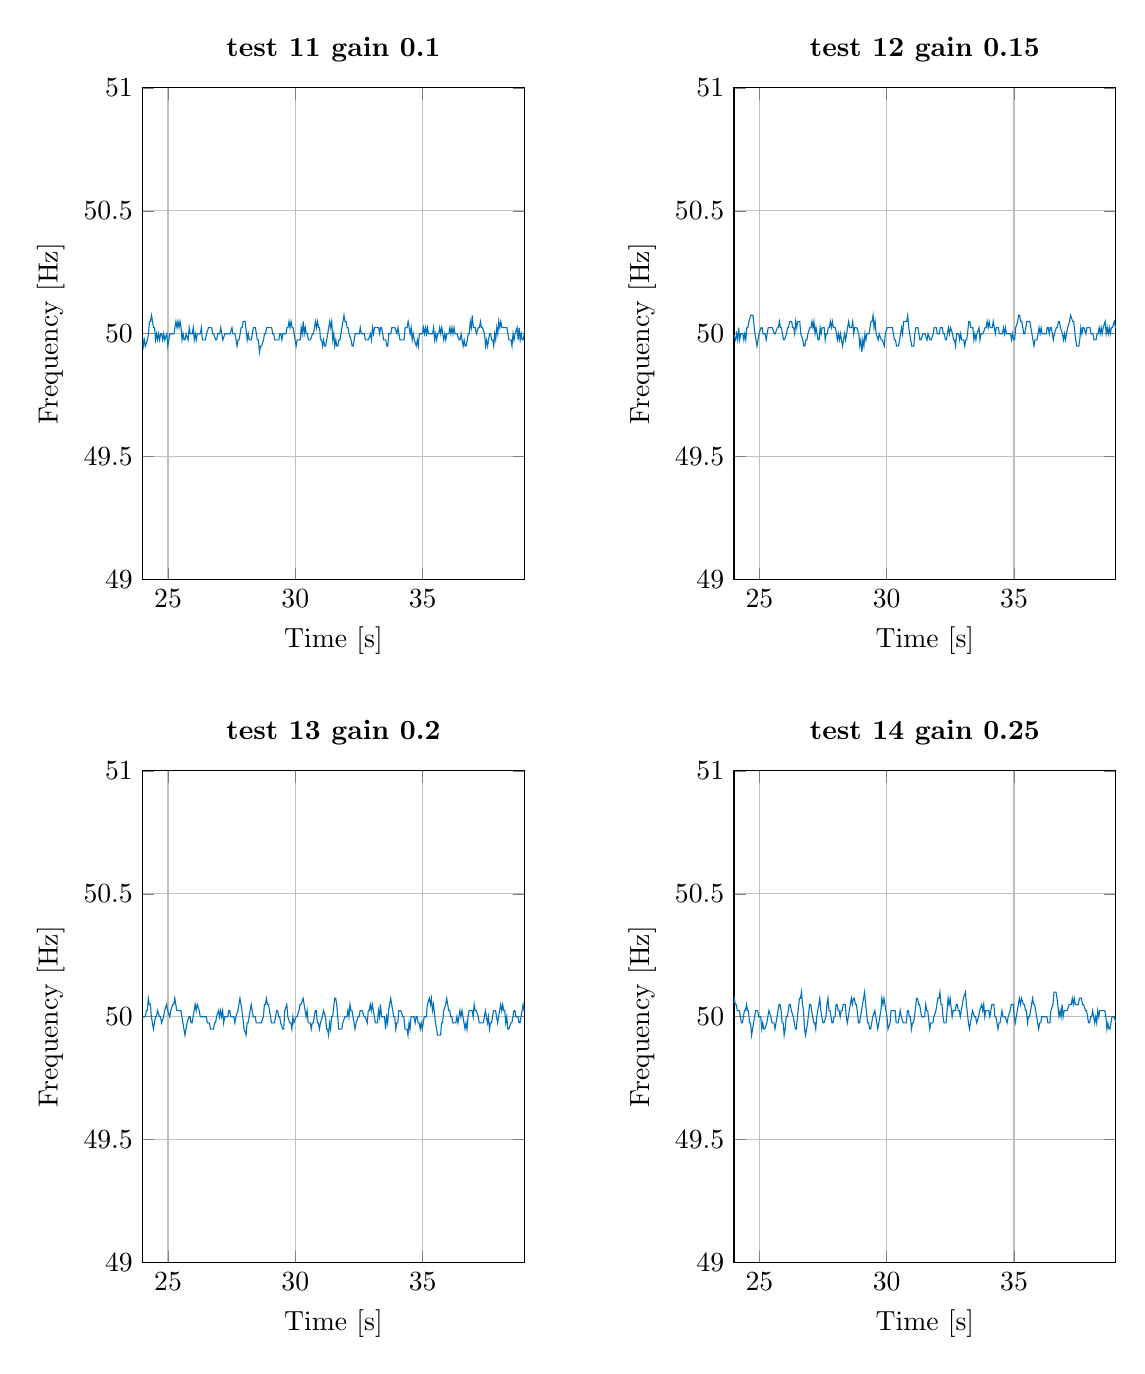
\begin{tikzpicture}

\begin{axis}[%
width=0.4\textwidth,
height=2.459in,
at={(1.043in,4.208in)},
scale only axis,
xmin=24,
xmax=39,
xlabel={Time [s]},
xmajorgrids,
ymin=49,
ymax=51,
ylabel={Frequency [Hz]},
ymajorgrids,
axis background/.style={fill=white},
title style={font=\bfseries},
title={test 11 gain 0.1}
]
\addplot [color=mycolor1,solid,forget plot]
  table[row sep=crcr]{%
23.99188	50.0000000000011\\
24.03188	49.9500499500485\\
24.07192	49.9750124937551\\
24.11194	49.9500499500485\\
24.19202	49.9750124937551\\
24.23204	50.0000000000011\\
24.27204	50.0500500500492\\
24.312	50.0500500500492\\
24.35196	50.0751126690062\\
24.43186	50.0250125062532\\
24.47184	50.0250125062532\\
24.51182	49.9750124937507\\
24.55184	50.0000000000011\\
24.59184	49.9750124937551\\
24.63186	49.9999999999966\\
24.67186	49.9750124937551\\
24.71188	50.0000000000011\\
24.75188	49.9999999999966\\
24.79188	49.9750124937551\\
24.8319	50.0000000000011\\
24.8719	49.9750124937507\\
24.95194	50.0000000000011\\
24.99194	49.9500499500485\\
25.072	50.0000000000011\\
25.112	50.0000000000011\\
25.192	49.9999999999966\\
25.232	50.0000000000011\\
25.31198	50.0500500500492\\
25.35194	50.0250125062532\\
25.39192	50.0500500500537\\
25.43188	50.0250125062488\\
25.47186	50.0500500500537\\
25.51182	50.0250125062532\\
25.5518	49.9750124937507\\
25.59182	50.0000000000011\\
25.63182	49.9750124937551\\
25.67184	49.9750124937507\\
25.71186	50.0000000000011\\
25.79186	49.9750124937507\\
25.83188	50.0250125062532\\
25.87186	50.0000000000011\\
25.95186	49.9999999999966\\
25.99186	50.0250125062532\\
26.03184	49.9750124937551\\
26.07186	50.0000000000011\\
26.11186	49.9750124937507\\
26.15188	50.0000000000011\\
26.23188	49.9999999999966\\
26.27188	50.0000000000011\\
26.31188	50.0250125062532\\
26.35186	49.9750124937551\\
26.39188	49.9750124937507\\
26.4319	49.9750124937551\\
26.47192	49.9750124937507\\
26.51194	50.0000000000011\\
26.59194	50.0250125062532\\
26.63192	50.0250125062532\\
26.71188	50.0250125062532\\
26.75186	50.0000000000011\\
26.79186	49.9999999999966\\
26.87188	49.9750124937507\\
26.9119	49.9750124937551\\
26.95192	50.0000000000011\\
26.99192	50.0000000000011\\
27.03192	49.9999999999966\\
27.07192	50.0250125062532\\
27.1119	50.0000000000011\\
27.1519	49.9750124937551\\
27.23192	50.0000000000011\\
27.27192	50.0000000000011\\
27.35192	49.9999999999966\\
27.39192	50.0000000000011\\
27.43192	50.0000000000011\\
27.51192	50.0250125062532\\
27.5519	49.9999999999966\\
27.5919	50.0000000000011\\
27.6319	50.0000000000011\\
27.6719	49.9750124937507\\
27.71192	49.9500499500529\\
27.75196	49.9750124937507\\
27.79198	49.9750124937551\\
27.872	50.0250125062532\\
27.91198	50.0250125062532\\
27.95196	50.0500500500492\\
27.99192	50.0500500500492\\
28.03188	50.0500500500492\\
28.1118	49.9750124937551\\
28.15182	50.0000000000011\\
28.19182	49.9750124937507\\
28.23184	49.9750124937551\\
28.27186	49.9750124937507\\
28.31188	50.0000000000011\\
28.35188	50.0250125062532\\
28.39186	50.0250125062532\\
28.43184	50.0250125062532\\
28.51182	49.9750124937507\\
28.55184	49.9750124937551\\
28.59186	49.9251123315022\\
28.63192	49.9500499500485\\
28.67196	49.9500499500529\\
28.75202	49.9750124937551\\
28.79204	49.9999999999966\\
28.83204	50.0000000000011\\
28.87204	50.0250125062532\\
28.91202	50.0250125062532\\
28.952	50.0250125062532\\
29.03196	50.0250125062532\\
29.07194	50.0250125062532\\
29.11192	50.0000000000011\\
29.15192	50.0000000000011\\
29.19192	49.9750124937507\\
29.23194	49.9750124937551\\
29.27196	49.9750124937507\\
29.31198	49.9750124937551\\
29.352	49.9750124937507\\
29.39202	50.0000000000011\\
29.43202	50.0000000000011\\
29.47202	49.9750124937507\\
29.51204	50.0000000000011\\
29.55204	50.0000000000011\\
29.63204	49.9999999999966\\
29.67204	50.0250125062532\\
29.71202	50.0250125062532\\
29.752	50.0500500500537\\
29.79196	50.0250125062532\\
29.83194	50.0500500500492\\
29.8719	50.0250125062532\\
29.91188	50.0250125062532\\
29.95186	49.9999999999966\\
30.03188	49.9500499500485\\
30.07192	49.9750124937551\\
30.11194	49.9750124937507\\
30.15196	49.9750124937551\\
30.19198	49.9750124937551\\
30.232	50.0250125062532\\
30.27198	49.9999999999966\\
30.31198	50.0500500500492\\
30.35194	50.0000000000011\\
30.39194	50.0250125062532\\
30.43192	50.0000000000011\\
30.47192	50.0000000000011\\
30.51192	49.9750124937507\\
30.55194	49.9750124937551\\
30.59196	49.9750124937507\\
30.672	50.0000000000011\\
30.712	49.9999999999966\\
30.79198	50.0500500500537\\
30.83194	50.0250125062532\\
30.87192	50.0500500500492\\
30.91188	50.0250125062532\\
30.95186	50.0250125062532\\
30.99184	49.9750124937507\\
31.03186	49.9750124937551\\
31.07188	49.9500499500485\\
31.11192	49.9750124937551\\
31.15194	49.9500499500485\\
31.19198	49.9500499500485\\
31.23202	49.9750124937551\\
31.31204	50.0250125062532\\
31.35202	50.0500500500492\\
31.39198	50.0250125062532\\
31.43196	50.0500500500492\\
31.47192	49.9750124937551\\
31.51194	49.9999999999966\\
31.55194	49.9500499500529\\
31.59198	49.9750124937507\\
31.632	49.9500499500529\\
31.67204	49.9500499500485\\
31.71208	49.9750124937507\\
31.7521	49.9750124937551\\
31.83212	50.0250125062532\\
31.8721	50.0500500500492\\
31.91206	50.0751126690017\\
31.952	50.0500500500492\\
31.99196	50.0500500500492\\
32.03192	50.0250125062532\\
32.0719	50.0250125062532\\
32.11188	50.0000000000011\\
32.19188	49.9750124937551\\
32.2319	49.9500499500529\\
32.27194	49.950049950044\\
32.352	50.0000000000011\\
32.392	50.0000000000011\\
32.472	49.9999999999922\\
32.512	50.0000000000011\\
32.552	50.0250125062532\\
32.59198	50.0000000000011\\
32.63198	50.0000000000011\\
32.71198	50.0000000000011\\
32.75198	49.9750124937551\\
32.792	49.9750124937463\\
32.83202	49.9750124937551\\
32.87204	49.9750124937551\\
32.95208	50.0000000000011\\
32.99208	49.9750124937463\\
33.0321	50.0250125062532\\
33.07208	50.0000000000011\\
33.11208	50.0250125062532\\
33.15206	50.0250125062532\\
33.23202	50.0250125062532\\
33.272	50.0250125062532\\
33.31198	50.0000000000011\\
33.35198	50.0250125062532\\
33.39196	50.0250125062532\\
33.47194	49.9750124937551\\
33.51196	49.9750124937463\\
33.55198	49.9750124937551\\
33.592	49.9500499500529\\
33.63204	49.9500499500529\\
33.67208	49.9999999999922\\
33.71208	50.0000000000011\\
33.75208	50.0000000000011\\
33.79208	50.0250125062532\\
33.87204	50.0250125062532\\
33.91202	50.0250125062532\\
33.99198	50.0000000000011\\
34.03198	50.0250125062532\\
34.11196	49.9750124937551\\
34.15198	49.9750124937463\\
34.192	49.9750124937551\\
34.23202	49.9750124937551\\
34.27204	49.9750124937551\\
34.31206	50.0250125062532\\
34.39202	50.0250125062532\\
34.432	50.0500500500492\\
34.51194	50.0000000000011\\
34.55194	50.0250125062532\\
34.59192	49.9750124937463\\
34.63194	50.0000000000011\\
34.67194	49.9750124937551\\
34.752	49.950049950044\\
34.79204	49.9750124937551\\
34.83206	49.9500499500529\\
34.8721	50.0000000000011\\
34.9121	50.0000000000011\\
34.9921	49.9999999999922\\
35.0321	50.0250125062532\\
35.07208	50.0000000000011\\
35.11208	50.0250125062532\\
35.15206	50.0000000000011\\
35.19206	50.0250125062532\\
35.23204	50.0000000000011\\
35.27204	50.0000000000011\\
35.31204	50.0000000000011\\
35.39204	50.0000000000011\\
35.43204	50.0250125062532\\
35.47202	49.9750124937463\\
35.51204	50.0000000000011\\
35.55204	49.9750124937551\\
35.59206	50.0000000000011\\
35.63206	50.0000000000011\\
35.67206	50.0250125062532\\
35.71204	50.0000000000011\\
35.75204	50.0250125062532\\
35.79202	49.9999999999922\\
35.83202	49.9750124937551\\
35.87204	50.0000000000011\\
35.91204	49.9750124937551\\
35.95206	50.0000000000011\\
36.03206	50.0000000000011\\
36.07206	50.0250125062444\\
36.11204	50.0000000000011\\
36.15204	50.0250125062532\\
36.19202	50.0000000000011\\
36.23202	50.0250125062532\\
36.272	50.0000000000011\\
36.312	50.0000000000011\\
36.352	50.0000000000011\\
36.432	49.9750124937551\\
36.47202	49.9750124937463\\
36.51204	50.0000000000011\\
36.55204	49.9750124937551\\
36.59206	49.9500499500529\\
36.6321	49.9750124937463\\
36.67212	49.9500499500529\\
36.71216	49.9500499500529\\
36.79222	49.9999999999922\\
36.83222	50.0000000000011\\
36.87222	50.0500500500492\\
36.91218	50.0250125062532\\
36.95216	50.0751126690106\\
36.9921	50.0250125062532\\
37.07206	50.0250125062532\\
37.11204	49.9999999999922\\
37.19204	50.0250125062532\\
37.23202	50.0250125062532\\
37.272	50.0500500500492\\
37.31196	50.0250125062532\\
37.35194	50.0250125062532\\
37.4319	50.0000000000011\\
37.4719	49.9500499500529\\
37.51194	49.9750124937551\\
37.55196	49.950049950044\\
37.592	49.9750124937551\\
37.63202	50.0000000000011\\
37.67202	50.0000000000011\\
37.71202	49.9750124937551\\
37.75204	49.9750124937463\\
37.79206	49.9500499500529\\
37.8321	50.0000000000011\\
37.8721	49.9750124937551\\
37.91212	50.0250125062532\\
37.9521	50.0000000000011\\
37.9921	50.0500500500492\\
38.03206	50.0250125062532\\
38.07204	50.0500500500492\\
38.112	50.0250125062532\\
38.19196	50.0250125062532\\
38.23194	50.0250125062532\\
38.3119	50.0250125062532\\
38.35188	50.0000000000011\\
38.39188	49.9750124937463\\
38.4319	49.9750124937551\\
38.47192	49.9750124937551\\
38.51194	49.9500499500529\\
38.55198	49.9999999999922\\
38.59198	49.9750124937551\\
38.632	50.0000000000011\\
38.712	50.0250125062532\\
38.75198	49.9750124937551\\
38.792	50.0250125062532\\
38.83198	49.9750124937463\\
38.872	50.0000000000011\\
38.912	49.9750124937551\\
38.95202	49.9750124937551\\
38.99204	50.0000000000011\\
39.03204	50.0250125062532\\
};
\end{axis}

\begin{axis}[%
width=0.4\textwidth,
height=2.459in,
at={(4in,4.208in)},
scale only axis,
xmin=24,
xmax=39,
xlabel={Time [s]},
xmajorgrids,
ymin=49,
ymax=51,
ylabel={Frequency [Hz]},
ymajorgrids,
axis background/.style={fill=white},
title style={font=\bfseries},
title={test 12  gain 0.15}
]
\addplot [color=mycolor1,solid,forget plot]
  table[row sep=crcr]{%
23.98552	50.0000000000011\\
24.06552	49.9750124937551\\
24.10554	50.0000000000011\\
24.14554	49.9750124937507\\
24.18556	50.0250125062532\\
24.22554	49.9750124937551\\
24.26556	50.0000000000011\\
24.30556	49.9999999999966\\
24.34556	50.0000000000011\\
24.38556	49.9750124937551\\
24.42558	49.9999999999966\\
24.46558	49.9750124937551\\
24.5056	50.0250125062532\\
24.54558	50.0250125062532\\
24.58556	50.0500500500492\\
24.66546	50.0751126690062\\
24.7054	50.0751126690017\\
24.74534	50.0751126690062\\
24.82524	50.0000000000011\\
24.86524	49.9750124937507\\
24.90526	49.9500499500485\\
24.9453	49.9750124937551\\
24.98532	50.0000000000011\\
25.06532	50.0250125062532\\
25.1053	50.0250125062532\\
25.14528	49.9999999999966\\
25.18528	50.0000000000011\\
25.22528	50.0000000000011\\
25.26528	49.9750124937507\\
25.3053	50.0000000000011\\
25.3453	50.0250125062532\\
25.38528	50.0250125062532\\
25.46524	50.0250125062532\\
25.50522	50.0250125062532\\
25.58518	50.0000000000011\\
25.62518	49.9999999999966\\
25.70518	50.0250125062532\\
25.74516	50.0250125062532\\
25.78514	50.0500500500492\\
25.8251	50.0250125062532\\
25.86508	50.0250125062532\\
25.94506	49.9750124937551\\
25.98508	49.9750124937507\\
26.06512	49.9999999999966\\
26.10512	50.0250125062532\\
26.1451	50.0250125062532\\
26.18508	50.0500500500537\\
26.22504	50.0500500500492\\
26.265	50.0500500500492\\
26.30496	50.0250125062532\\
26.34494	50.0250125062532\\
26.38492	50.0000000000011\\
26.42492	50.0500500500492\\
26.46488	50.0250125062532\\
26.50486	50.0500500500492\\
26.58478	50.0500500500492\\
26.62474	50.0000000000011\\
26.70474	49.9750124937507\\
26.74476	49.9500499500529\\
26.7848	49.9500499500485\\
26.82484	49.9750124937551\\
26.86486	49.9750124937507\\
26.90488	50.0000000000011\\
26.98488	50.0250125062532\\
27.02486	50.0250125062532\\
27.06484	50.0500500500492\\
27.1048	50.0250125062532\\
27.14478	50.0500500500492\\
27.18474	50.0000000000011\\
27.22474	50.0250125062532\\
27.26472	50.0000000000011\\
27.30472	49.9750124937507\\
27.34474	49.9750124937551\\
27.38476	50.0250125062532\\
27.42474	49.9999999999966\\
27.46474	50.0250125062532\\
27.50472	50.0250125062532\\
27.5447	50.0250125062532\\
27.58468	49.9750124937551\\
27.6247	50.0000000000011\\
27.6647	49.9999999999966\\
27.7047	50.0250125062532\\
27.74468	50.0250125062532\\
27.78466	50.0500500500537\\
27.82462	50.0250125062532\\
27.8646	50.0500500500492\\
27.90456	50.0250125062532\\
27.98452	50.0250125062532\\
28.0245	49.9999999999966\\
28.0645	49.9750124937551\\
28.10452	50.0000000000011\\
28.14452	49.9750124937507\\
28.18454	50.0000000000011\\
28.26456	49.9500499500485\\
28.3046	49.9750124937507\\
28.34462	50.0000000000011\\
28.38462	49.9750124937551\\
28.42464	49.9999999999966\\
28.50464	50.0500500500492\\
28.5446	50.0250125062532\\
28.62456	50.0250125062532\\
28.66454	50.0500500500537\\
28.7045	49.9999999999966\\
28.7445	50.0250125062532\\
28.78448	50.0250125062532\\
28.82446	50.0250125062532\\
28.90442	50.0000000000011\\
28.94442	49.9500499500485\\
28.98446	49.9750124937551\\
29.02448	49.9251123315022\\
29.06454	49.9750124937551\\
29.10456	49.9500499500485\\
29.1446	50.0000000000011\\
29.1846	49.9750124937507\\
29.22462	50.0000000000011\\
29.26462	50.0000000000011\\
29.30462	49.9999999999966\\
29.38462	50.0500500500492\\
29.42458	50.0500500500537\\
29.46454	50.0751126690017\\
29.50448	50.0250125062532\\
29.54446	50.0500500500492\\
29.58442	50.0000000000011\\
29.66442	49.9750124937507\\
29.70444	50.0000000000011\\
29.78446	49.9750124937507\\
29.82448	49.9750124937551\\
29.90452	49.9500499500529\\
29.94456	49.9999999999966\\
30.02456	50.0250125062532\\
30.06454	50.0250125062532\\
30.1445	50.0250125062532\\
30.18448	50.0250125062532\\
30.22446	50.0250125062532\\
30.30442	49.9750124937507\\
30.34444	49.9750124937551\\
30.38446	49.9500499500485\\
30.4245	49.9500499500529\\
30.46454	49.9500499500485\\
30.5446	50.0000000000011\\
30.5846	50.0250125062532\\
30.62458	50.0000000000011\\
30.66458	50.0500500500492\\
30.70454	50.0500500500492\\
30.7445	50.0500500500537\\
30.78446	50.0500500500492\\
30.82442	50.0751126690017\\
30.86436	50.0250125062532\\
30.94432	49.9750124937551\\
30.98434	49.9500499500485\\
31.06442	49.9500499500529\\
31.10446	49.9999999999966\\
31.14446	50.0250125062532\\
31.18444	50.0250125062532\\
31.22442	50.0250125062532\\
31.3044	49.9750124937551\\
31.34442	49.9750124937507\\
31.42446	49.9999999999966\\
31.46446	50.0000000000011\\
31.50446	50.0000000000011\\
31.58446	49.9750124937507\\
31.62448	50.0000000000011\\
31.7045	49.9750124937507\\
31.74452	49.9750124937551\\
31.82454	50.0000000000011\\
31.86454	50.0250125062532\\
31.9445	50.0250125062532\\
31.98448	50.0000000000011\\
32.06448	50.0000000000011\\
32.10448	50.0250125062532\\
32.18444	50.0250125062532\\
32.22442	50.0000000000011\\
32.26442	49.9999999999922\\
32.30442	49.9750124937551\\
32.34444	49.9750124937551\\
32.38446	50.0000000000011\\
32.42446	50.0250125062532\\
32.46444	50.0000000000011\\
32.50444	50.0250125062532\\
32.5844	50.0000000000011\\
32.6244	49.9750124937463\\
32.66442	49.9750124937551\\
32.70444	49.9500499500529\\
32.74448	50.0000000000011\\
32.82448	49.9999999999922\\
32.86448	49.9750124937551\\
32.9045	50.0000000000011\\
32.9445	49.9750124937551\\
32.98452	49.9750124937551\\
33.02454	49.9750124937463\\
33.06456	49.9500499500529\\
33.1046	49.9750124937551\\
33.14462	49.9750124937551\\
33.22464	50.0500500500492\\
33.2646	50.0500500500492\\
33.30456	50.0250125062532\\
33.34454	50.0250125062532\\
33.38452	50.0250125062532\\
33.4245	49.9750124937463\\
33.46452	50.0000000000011\\
33.50452	49.9750124937551\\
33.54454	50.0000000000011\\
33.62454	50.0250125062532\\
33.66452	49.9750124937551\\
33.70454	50.0000000000011\\
33.74454	49.9999999999922\\
33.78454	50.0000000000011\\
33.86454	50.0250125062532\\
33.90452	50.0250125062532\\
33.9445	50.0500500500492\\
33.98446	50.0250125062532\\
34.02444	50.0500500500492\\
34.0644	50.0250125062532\\
34.10438	50.0250125062532\\
34.14436	50.0250125062532\\
34.18434	50.0500500500492\\
34.2243	50.0250125062532\\
34.26428	50.0000000000011\\
34.30428	50.0250125062532\\
34.38424	50.0250125062532\\
34.42422	50.0000000000011\\
34.50422	50.0000000000011\\
34.54422	50.0000000000011\\
34.58422	50.0250125062532\\
34.6242	50.0000000000011\\
34.6642	50.0250125062532\\
34.70418	49.9999999999922\\
34.74418	50.0000000000011\\
34.78418	50.0000000000011\\
34.86418	50.0000000000011\\
34.90418	49.9750124937551\\
34.9442	50.0000000000011\\
34.9842	49.9750124937463\\
35.02422	49.9750124937551\\
35.06424	50.0250125062532\\
35.1442	50.0500500500492\\
35.18416	50.0751126690017\\
35.2241	50.0751126690106\\
35.26404	50.0500500500492\\
35.304	50.0500500500492\\
35.38394	50.0000000000011\\
35.42394	50.0000000000011\\
35.50392	50.0500500500492\\
35.54388	50.0500500500492\\
35.6238	50.0500500500492\\
35.66376	50.0250125062532\\
35.70374	50.0000000000011\\
35.78376	49.950049950044\\
35.8238	49.9750124937551\\
35.90384	49.9750124937551\\
35.94386	49.9999999999922\\
35.98386	50.0250125062532\\
36.02384	50.0000000000011\\
36.06384	50.0250125062532\\
36.10382	50.0000000000011\\
36.14382	50.0000000000011\\
36.18382	50.0000000000011\\
36.26382	50.0000000000011\\
36.30382	50.0250125062532\\
36.3438	50.0250125062532\\
36.38378	50.0000000000011\\
36.42378	50.0250125062532\\
36.46376	50.0250125062532\\
36.54374	49.9750124937551\\
36.58376	50.0000000000011\\
36.66376	50.0250125062532\\
36.70374	50.0250125062532\\
36.74372	50.0500500500492\\
36.78368	50.0500500500492\\
36.82364	50.0250125062532\\
36.9036	50.0000000000011\\
36.9436	49.9750124937551\\
36.98362	50.0000000000011\\
37.02362	49.9750124937463\\
37.06364	50.0000000000011\\
37.10364	50.0250125062532\\
37.1836	50.0500500500492\\
37.22356	50.0751126690106\\
37.30344	50.0500500500492\\
37.3434	50.0500500500492\\
37.42336	49.9750124937551\\
37.46338	49.950049950044\\
37.50342	49.9500499500529\\
37.54346	49.9500499500529\\
37.5835	49.9750124937463\\
37.62352	50.0250125062532\\
37.6635	50.0000000000011\\
37.7035	50.0250125062532\\
37.74348	50.0250125062532\\
37.82344	50.0000000000011\\
37.86344	50.0250125062532\\
37.9434	50.0250125062532\\
37.98338	50.0250125062532\\
38.02336	50.0000000000011\\
38.06336	50.0000000000011\\
38.10336	50.0000000000011\\
38.14336	49.9750124937463\\
38.18338	49.9750124937551\\
38.2234	49.9750124937551\\
38.26342	50.0000000000011\\
38.30342	50.0000000000011\\
38.34342	50.0250125062532\\
38.3834	50.0000000000011\\
38.4234	50.0250125062532\\
38.46338	49.9999999999922\\
38.50338	50.0250125062532\\
38.58334	50.0500500500581\\
38.6233	49.9999999999922\\
38.6633	50.0250125062532\\
38.70328	50.0000000000011\\
38.74328	50.0250125062532\\
38.78326	50.0000000000011\\
38.82326	50.0250125062532\\
38.86324	50.0250125062532\\
38.9432	50.0500500500492\\
38.98316	50.0250125062532\\
39.02314	50.0250125062532\\
};
\end{axis}

\begin{axis}[%
width=0.4\textwidth,
height=2.459in,
at={(1.043in,0.793in)},
scale only axis,
xmin=24,
xmax=39,
xlabel={Time [s]},
xmajorgrids,
ymin=49,
ymax=51,
ylabel={Frequency [Hz]},
ymajorgrids,
axis background/.style={fill=white},
title style={font=\bfseries},
title={test 13  gain 0.2}
]
\addplot [color=mycolor1,solid,forget plot]
  table[row sep=crcr]{%
23.98652	50.0000000000011\\
24.06652	50.0000000000011\\
24.10652	49.9999999999966\\
24.14652	50.0250125062532\\
24.1865	50.0250125062532\\
24.22648	50.0751126690062\\
24.26642	50.0500500500492\\
24.30638	50.0500500500492\\
24.34634	50.0000000000011\\
24.42634	49.9500499500485\\
24.46638	49.9750124937507\\
24.5064	50.0000000000011\\
24.5464	50.0000000000011\\
24.5864	50.0250125062532\\
24.66638	49.9999999999966\\
24.70638	50.0000000000011\\
24.74638	49.9750124937551\\
24.8264	50.0000000000011\\
24.8664	50.0250125062532\\
24.94636	50.0500500500492\\
24.98632	50.0250125062532\\
25.06628	50.0000000000011\\
25.10628	50.0250125062532\\
25.18624	50.0500500500492\\
25.2262	50.0500500500492\\
25.26616	50.0751126690062\\
25.3061	50.0500500500492\\
25.34606	50.0250125062532\\
25.38604	50.0250125062532\\
25.466	50.0250125062532\\
25.50598	50.0250125062532\\
25.58596	49.9750124937507\\
25.62598	49.9500499500529\\
25.66602	49.9251123315022\\
25.70608	49.9500499500485\\
25.74612	49.9750124937551\\
25.82614	50.0000000000011\\
25.86614	50.0000000000011\\
25.90614	49.9750124937507\\
25.94616	49.9750124937551\\
25.98618	50.0000000000011\\
26.06616	50.0500500500492\\
26.10612	50.0250125062532\\
26.1461	50.0500500500492\\
26.22602	50.0250125062532\\
26.266	50.0000000000011\\
26.346	49.9999999999966\\
26.386	50.0000000000011\\
26.466	50.0000000000011\\
26.506	49.9999999999966\\
26.546	49.9750124937551\\
26.58602	49.9750124937551\\
26.62604	49.9750124937507\\
26.66606	49.9500499500485\\
26.7061	49.9500499500529\\
26.74614	49.9500499500485\\
26.78618	49.9500499500485\\
26.82622	49.9750124937551\\
26.86624	49.9750124937551\\
26.90626	49.9999999999966\\
26.98626	50.0250125062532\\
27.02624	50.0000000000011\\
27.06624	50.0250125062532\\
27.10622	50.0000000000011\\
27.14622	50.0250125062532\\
27.1862	49.9750124937507\\
27.22622	50.0000000000011\\
27.26622	50.0000000000011\\
27.30622	49.9999999999966\\
27.34622	50.0000000000011\\
27.38622	50.0250125062532\\
27.4262	50.0250125062532\\
27.46618	50.0000000000011\\
27.50618	50.0000000000011\\
27.54618	49.9999999999966\\
27.58618	50.0000000000011\\
27.62618	49.9750124937551\\
27.6662	49.9999999999966\\
27.7462	50.0250125062532\\
27.78618	50.0500500500492\\
27.82614	50.0751126690062\\
27.86608	50.0500500500492\\
27.90604	50.0250125062532\\
27.98602	49.9500499500485\\
28.0661	49.9251123315022\\
28.10616	49.9750124937551\\
28.14618	49.9750124937551\\
28.1862	49.9999999999966\\
28.26618	50.0500500500492\\
28.30614	50.0250125062532\\
28.34612	50.0000000000011\\
28.38612	50.0000000000011\\
28.42612	50.0000000000011\\
28.46612	49.9750124937507\\
28.50614	49.9750124937551\\
28.54616	49.9750124937507\\
28.58618	49.9750124937551\\
28.6262	49.9750124937507\\
28.66622	49.9750124937551\\
28.74626	49.9999999999966\\
28.78626	50.0500500500537\\
28.82622	50.0500500500492\\
28.86618	50.0751126690017\\
28.90612	50.0500500500492\\
28.94608	50.0500500500492\\
29.02602	50.0000000000011\\
29.06602	49.9750124937551\\
29.10604	49.9750124937507\\
29.14606	49.9750124937551\\
29.18608	49.9750124937507\\
29.2661	50.0250125062532\\
29.30608	50.0250125062532\\
29.34606	50.0000000000011\\
29.38606	50.0000000000011\\
29.42606	49.9750124937507\\
29.50612	49.9500499500485\\
29.54616	49.9500499500485\\
29.5862	50.0250125062532\\
29.66616	50.0500500500492\\
29.70612	50.0000000000011\\
29.78612	49.9750124937507\\
29.82614	49.9750124937551\\
29.86616	49.9500499500485\\
29.9062	50.0000000000011\\
29.9462	49.9750124937551\\
30.02622	50.0000000000011\\
30.06622	50.0000000000011\\
30.14622	50.0250125062532\\
30.1862	50.0500500500492\\
30.22616	50.0500500500492\\
30.30606	50.0751126690062\\
30.346	50.0500500500492\\
30.42592	50.0000000000011\\
30.46592	50.0250125062532\\
30.5059	49.9750124937507\\
30.54592	49.9750124937551\\
30.58594	49.9750124937551\\
30.62596	49.9500499500485\\
30.666	49.9750124937507\\
30.70602	49.9750124937551\\
30.78604	50.0250125062532\\
30.82602	50.0250125062532\\
30.866	49.9750124937507\\
30.90602	49.9750124937551\\
30.94604	49.9500499500485\\
30.98608	49.9750124937551\\
31.0661	50.0000000000011\\
31.1061	50.0250125062532\\
31.18606	50.0000000000011\\
31.22606	49.9500499500485\\
31.2661	49.9500499500529\\
31.30614	49.9251123315022\\
31.3462	49.9750124937507\\
31.38622	49.9500499500529\\
31.42626	49.9999999999966\\
31.46626	50.0000000000011\\
31.54622	50.0751126690062\\
31.58616	50.0751126690017\\
31.6261	50.0500500500492\\
31.70604	49.9500499500529\\
31.74608	49.9500499500485\\
31.82616	49.9500499500529\\
31.8662	49.9750124937507\\
31.94624	49.9999999999966\\
31.98624	50.0000000000055\\
32.02624	49.9999999999922\\
32.06624	50.0250125062532\\
32.10622	50.0000000000011\\
32.14622	50.0500500500492\\
32.18618	50.0250125062532\\
32.22616	50.0250125062532\\
32.26614	50.0000000000011\\
32.34616	49.9500499500529\\
32.3862	49.9750124937463\\
32.46624	50.0000000000011\\
32.50624	50.0000000000011\\
32.54624	50.0250125062532\\
32.58622	50.0250125062532\\
32.6262	50.0250125062532\\
32.70616	50.0000000000011\\
32.74616	50.0000000000011\\
32.82616	49.9750124937463\\
32.86618	50.0250125062532\\
32.90616	50.0250125062532\\
32.94614	50.0500500500492\\
32.9861	50.0250125062532\\
33.02608	50.0500500500581\\
33.10602	49.9999999999922\\
33.14602	49.9750124937551\\
33.22606	49.9750124937551\\
33.26608	50.0250125062532\\
33.30606	50.0000000000011\\
33.34606	50.0500500500492\\
33.38602	50.0000000000011\\
33.42602	49.9999999999922\\
33.46602	50.0000000000011\\
33.50602	50.0000000000011\\
33.54602	49.9500499500529\\
33.58606	50.0000000000011\\
33.62606	49.9750124937551\\
33.66608	50.0250125062532\\
33.74604	50.0751126690017\\
33.78598	50.0500500500492\\
33.86592	50.0000000000011\\
33.90592	50.0000000000011\\
33.94592	49.950049950044\\
33.98596	49.9750124937551\\
34.02598	49.9750124937551\\
34.066	50.0250125062532\\
34.10598	50.0250125062532\\
34.14596	50.0250125062532\\
34.22592	50.0000000000011\\
34.26592	49.9999999999922\\
34.30592	49.9500499500529\\
34.386	49.950049950044\\
34.42604	49.9251123315066\\
34.4661	49.9750124937551\\
34.50612	49.950049950044\\
34.54616	50.0000000000011\\
34.62616	50.0000000000011\\
34.66616	50.0000000000011\\
34.70616	49.9750124937551\\
34.74618	50.0000000000011\\
34.78618	50.0000000000011\\
34.82618	49.9750124937463\\
34.8662	49.9750124937551\\
34.90622	49.9500499500529\\
34.94626	49.9750124937551\\
34.98628	49.950049950044\\
35.02632	49.9750124937551\\
35.06634	50.0000000000011\\
35.14634	50.0000000000011\\
35.18634	50.0500500500492\\
35.26626	50.0751126690017\\
35.3062	50.0500500500492\\
35.34616	50.0751126690017\\
35.3861	50.0250125062532\\
35.42608	50.0500500500492\\
35.50604	49.9750124937551\\
35.54606	49.9500499500529\\
35.5861	49.9251123314978\\
35.62616	49.9251123315066\\
35.66622	49.9251123314978\\
35.70628	49.9251123315066\\
35.74634	49.9750124937551\\
35.78636	49.9750124937463\\
35.82638	50.0250125062532\\
35.90634	50.0500500500581\\
35.9463	50.0751126690017\\
36.0262	50.0250125062532\\
36.06618	50.0250125062532\\
36.10616	50.0000000000011\\
36.14616	50.0000000000011\\
36.18616	49.9750124937463\\
36.22618	49.9750124937551\\
36.2662	49.9750124937551\\
36.30622	49.9750124937551\\
36.34624	50.0000000000011\\
36.38624	49.9750124937463\\
36.42626	50.0000000000011\\
36.46626	50.0250125062532\\
36.50624	50.0000000000011\\
36.54624	50.0250125062532\\
36.58622	50.0000000000011\\
36.66622	49.950049950044\\
36.70626	49.9750124937551\\
36.74628	49.9500499500529\\
36.78632	50.0000000000011\\
36.82632	50.0250125062532\\
36.90628	50.0250125062532\\
36.94626	50.0250125062532\\
36.98624	50.0000000000011\\
37.02624	50.0500500500492\\
37.0662	50.0250125062532\\
37.10618	50.0250125062532\\
37.18616	49.9999999999922\\
37.22616	49.9750124937551\\
37.3062	49.9750124937551\\
37.38624	49.9750124937463\\
37.42626	50.0000000000011\\
37.46626	50.0250125062532\\
37.54624	49.9750124937551\\
37.58626	50.0000000000011\\
37.62626	49.950049950044\\
37.6663	49.9750124937551\\
37.70632	49.9750124937551\\
37.74634	50.0000000000011\\
37.78634	50.0250125062532\\
37.82632	50.0250125062532\\
37.8663	50.0250125062532\\
37.94628	49.9750124937463\\
37.9863	50.0000000000011\\
38.0663	50.0500500500492\\
38.10626	50.0250125062532\\
38.14624	50.0500500500492\\
38.1862	50.0250125062532\\
38.22618	50.0250125062532\\
38.26616	49.9750124937551\\
38.30618	50.0000000000011\\
38.34618	49.9500499500529\\
38.38622	49.950049950044\\
38.4663	49.9750124937551\\
38.50632	49.9750124937551\\
38.58634	50.0250125062532\\
38.62632	50.0250125062532\\
38.6663	50.0000000000011\\
38.7063	50.0000000000011\\
38.7463	50.0000000000011\\
38.7863	49.9750124937551\\
38.82632	49.9750124937551\\
38.86634	50.0000000000011\\
38.94632	50.0500500500581\\
38.98628	50.0250125062532\\
39.02626	50.0500500500492\\
};
\end{axis}

\begin{axis}[%
width=0.4\textwidth,
height=2.459in,
at={(4in,0.793in)},
scale only axis,
xmin=24,
xmax=39,
xlabel={Time [s]},
xmajorgrids,
ymin=49,
ymax=51,
ylabel={Frequency [Hz]},
ymajorgrids,
axis background/.style={fill=white},
title style={font=\bfseries},
title={test 14  gain 0.25}
]
\addplot [color=mycolor1,solid,forget plot]
  table[row sep=crcr]{%
23.97254	50.0500500500492\\
24.0125	50.0751126690062\\
24.05244	50.0500500500492\\
24.0924	50.0500500500492\\
24.13236	50.0250125062532\\
24.17234	50.0250125062532\\
24.21232	50.0250125062532\\
24.29232	49.9750124937507\\
24.33234	49.9750124937551\\
24.41236	50.0250125062532\\
24.45234	50.0250125062532\\
24.49232	50.0500500500537\\
24.53228	50.0250125062532\\
24.57226	50.0250125062532\\
24.61224	49.9750124937507\\
24.65226	49.9750124937551\\
24.69228	49.9251123315022\\
24.73234	49.9500499500485\\
24.8124	49.9999999999966\\
24.8524	50.0250125062532\\
24.93236	50.0250125062532\\
24.97234	50.0000000000011\\
25.05234	50.0000000000011\\
25.09234	49.9500499500485\\
25.13238	49.9750124937551\\
25.1724	49.9500499500485\\
25.21244	49.9500499500485\\
25.29252	49.9750124937507\\
25.33254	50.0000000000011\\
25.37254	50.0250125062532\\
25.45252	49.9999999999966\\
25.49252	49.9750124937551\\
25.53254	49.9750124937507\\
25.57256	49.9750124937551\\
25.61258	49.9500499500485\\
25.69264	50.0000000000011\\
25.73264	50.0250125062532\\
25.77262	50.0500500500492\\
25.81258	50.0500500500492\\
25.85254	50.0250125062532\\
25.89252	49.9750124937507\\
25.93254	49.9750124937551\\
25.97256	49.9251123315022\\
26.01262	49.9500499500485\\
26.05266	50.0000000000011\\
26.09266	50.0000000000011\\
26.13266	50.0250125062532\\
26.17264	50.0500500500492\\
26.2126	50.0500500500492\\
26.25256	50.0250125062532\\
26.33252	50.0000000000011\\
26.37252	49.9750124937551\\
26.41254	49.9500499500485\\
26.45258	49.9500499500485\\
26.49262	50.0000000000011\\
26.57262	50.0751126690017\\
26.61256	50.0751126690062\\
26.6525	50.1002004007989\\
26.69242	50.0500500500492\\
26.73238	50.0250125062532\\
26.77236	49.9500499500529\\
26.8124	49.9251123315022\\
26.85246	49.9500499500485\\
26.8925	49.9750124937551\\
26.97252	50.0500500500537\\
27.01248	50.0500500500492\\
27.09242	50.0000000000011\\
27.13242	49.9750124937507\\
27.17244	49.9750124937551\\
27.21246	49.9500499500485\\
27.2525	50.0000000000011\\
27.33248	50.0500500500492\\
27.37244	50.0751126690017\\
27.41238	50.0250125062532\\
27.49234	49.9750124937551\\
27.53236	49.9750124937507\\
27.6124	50.0000000000011\\
27.6524	50.0500500500492\\
27.69236	50.0751126690017\\
27.7323	50.0250125062532\\
27.77228	50.0250125062532\\
27.85228	49.9750124937507\\
27.8923	49.9750124937551\\
27.93232	50.0000000000011\\
27.97232	49.9999999999966\\
28.01232	50.0500500500537\\
28.05228	50.0500500500492\\
28.09224	50.0250125062532\\
28.13222	50.0250125062532\\
28.1722	49.9999999999966\\
28.2122	50.0250125062532\\
28.25218	50.0250125062532\\
28.29216	50.0500500500537\\
28.33212	50.0500500500492\\
28.37208	50.0500500500492\\
28.41204	50.0000000000011\\
28.45204	49.9750124937507\\
28.49206	50.0000000000011\\
28.53206	50.0250125062532\\
28.61202	50.0751126690017\\
28.65196	50.0500500500537\\
28.69192	50.0751126690017\\
28.73186	50.0751126690017\\
28.7718	50.0500500500537\\
28.81176	50.0500500500492\\
28.89172	49.9750124937507\\
28.93174	49.9750124937551\\
29.01176	50.0250125062532\\
29.05174	50.0500500500537\\
29.13164	50.1002004008033\\
29.17156	50.0500500500492\\
29.25148	49.9750124937507\\
29.2915	49.9750124937551\\
29.33152	49.9500499500485\\
29.37156	49.9500499500529\\
29.4116	49.9750124937507\\
29.45162	50.0000000000011\\
29.53162	50.0250125062532\\
29.5716	50.0000000000011\\
29.65162	49.9500499500485\\
29.69166	49.9750124937551\\
29.77168	50.0250125062532\\
29.81166	50.0751126690017\\
29.8516	50.0500500500492\\
29.89156	50.0751126690062\\
29.9315	50.0500500500492\\
30.01146	49.9999999999966\\
30.05146	49.9500499500529\\
30.13152	49.9750124937551\\
30.17154	50.0250125062532\\
30.21152	50.0250125062532\\
30.29148	50.0250125062532\\
30.33146	50.0250125062532\\
30.37144	49.9750124937507\\
30.41146	49.9750124937551\\
30.45148	49.9750124937507\\
30.53152	50.0250125062532\\
30.5715	50.0000000000011\\
30.6515	49.9750124937551\\
30.69152	49.9750124937507\\
30.73154	49.9750124937551\\
30.77156	49.9750124937551\\
30.81158	50.0250125062532\\
30.85156	50.0250125062532\\
30.89154	49.9999999999966\\
30.93154	50.0000000000011\\
30.97154	49.9500499500485\\
31.01158	49.9750124937551\\
31.0516	49.9750124937507\\
31.09162	50.0000000000011\\
31.17158	50.0751126690062\\
31.21152	50.0751126690017\\
31.25146	50.0500500500492\\
31.29142	50.0500500500537\\
31.33138	50.0250125062532\\
31.37136	49.9999999999966\\
31.41136	50.0000000000011\\
31.45136	50.0000000000011\\
31.49136	50.0000000000011\\
31.53136	50.0500500500492\\
31.57132	50.0250125062532\\
31.6113	50.0250125062532\\
31.6913	49.9500499500529\\
31.73134	49.9750124937507\\
31.77136	49.9750124937551\\
31.81138	49.9750124937507\\
31.8514	50.0000000000011\\
31.9314	50.0250125062532\\
31.97138	50.0500500500492\\
32.01134	50.0751126690017\\
32.05128	50.0751126690017\\
32.09122	50.1002004008078\\
32.13114	50.0500500500492\\
32.1711	50.0500500500492\\
32.21106	50.0000000000011\\
32.25106	49.9750124937551\\
32.29108	49.9750124937463\\
32.3311	49.9750124937551\\
32.37112	50.0250125062532\\
32.4111	50.0751126690017\\
32.45104	50.0500500500492\\
32.491	50.0751126690106\\
32.57092	49.9999999999922\\
32.61092	50.0250125062532\\
32.69088	50.0250125062532\\
32.73086	50.0500500500492\\
32.77082	50.0500500500581\\
32.81078	50.0250125062532\\
32.85076	50.0250125062532\\
32.89074	49.9999999999922\\
32.97072	50.0500500500581\\
33.01068	50.0751126690017\\
33.09056	50.1002004007989\\
33.13048	50.0500500500492\\
33.21044	49.9750124937551\\
33.25046	49.9500499500529\\
33.33052	50.0000000000011\\
33.37052	50.0250125062532\\
33.45048	50.0000000000011\\
33.49048	50.0000000000011\\
33.53048	49.9750124937551\\
33.61052	49.9999999999922\\
33.65052	50.0250125062532\\
33.73048	50.0500500500581\\
33.77044	50.0250125062444\\
33.81042	50.0500500500581\\
33.85038	49.9999999999922\\
33.89038	50.0250125062532\\
33.97034	50.0250125062532\\
34.01032	50.0250125062532\\
34.0503	50.0000000000011\\
34.0903	50.0250125062532\\
34.13028	50.0500500500492\\
34.2102	50.0500500500581\\
34.25016	49.9999999999922\\
34.29016	50.0000000000011\\
34.37018	49.9500499500529\\
34.41022	49.9750124937551\\
34.45024	49.9750124937463\\
34.49026	50.0000000000011\\
34.53026	50.0250125062532\\
34.57024	50.0000000000011\\
34.61024	50.0000000000011\\
34.65024	50.0000000000011\\
34.73024	49.9750124937463\\
34.77026	50.0000000000011\\
34.85026	50.0250125062532\\
34.89024	50.0500500500492\\
34.97016	50.0500500500581\\
35.01012	49.9999999999922\\
35.05012	49.9750124937551\\
35.13014	50.0250125062532\\
35.17012	50.0500500500492\\
35.21008	50.0751126690017\\
35.25002	50.0500500500492\\
35.28998	50.0751126690106\\
35.36986	50.0500500500492\\
35.40982	50.0500500500492\\
35.44978	50.0250125062532\\
35.48976	50.0250125062532\\
35.52974	49.9750124937551\\
35.56976	50.0000000000011\\
35.60976	50.0000000000011\\
35.64976	50.0250125062532\\
35.68974	50.0500500500492\\
35.7297	50.0751126690017\\
35.76964	50.0500500500492\\
35.8096	50.0500500500492\\
35.88954	50.0000000000011\\
35.92954	49.9750124937551\\
35.96956	49.950049950044\\
36.0096	49.9750124937551\\
36.04962	49.9750124937551\\
36.08964	50.0000000000011\\
36.12964	50.0000000000011\\
36.16964	49.9999999999922\\
36.20964	50.0000000000011\\
36.24964	50.0000000000011\\
36.28964	50.0000000000011\\
36.32964	49.9750124937551\\
36.40968	49.9750124937463\\
36.4497	50.0250125062532\\
36.52966	50.0500500500581\\
36.56962	50.1002004007989\\
36.64946	50.1002004007989\\
36.68938	50.0751126690106\\
36.76928	50.0000000000011\\
36.80928	50.0250125062532\\
36.84926	49.9999999999922\\
36.88926	50.0500500500581\\
36.92922	49.9999999999922\\
36.96922	50.0250125062532\\
37.04918	50.0250125062532\\
37.08916	50.0250125062532\\
37.16912	50.0500500500492\\
37.20908	50.0500500500581\\
37.24904	50.0500500500492\\
37.289	50.0751126690017\\
37.32894	50.0500500500492\\
37.3689	50.0751126690017\\
37.40884	50.0500500500492\\
37.4488	50.0500500500492\\
37.52872	50.0500500500581\\
37.56868	50.0751126690017\\
37.64856	50.0751126690017\\
37.6885	50.0500500500492\\
37.72846	50.0500500500492\\
37.80838	50.0250125062532\\
37.84836	50.0250125062532\\
37.92834	49.9750124937551\\
37.96836	49.9750124937551\\
38.00838	50.0000000000011\\
38.04838	50.0000000000011\\
38.08838	50.0250125062532\\
38.16834	49.9750124937463\\
38.20836	50.0000000000011\\
38.24836	49.9750124937551\\
38.28838	50.0250125062532\\
38.32836	50.0000000000011\\
38.36836	50.0250125062532\\
38.44832	50.0250125062532\\
38.4883	50.0250125062532\\
38.56826	50.0250125062532\\
38.60824	50.0000000000011\\
38.64824	49.950049950044\\
38.68828	49.9750124937551\\
38.7283	49.9500499500529\\
38.76834	49.950049950044\\
38.80838	49.9750124937551\\
38.8484	50.0000000000011\\
38.9284	50.0000000000011\\
39.0084	49.9750124937463\\
};
\end{axis}
\end{tikzpicture}%
\caption{Steady state at 20 kW load, with various scaling factors.}
\label{fig:test11-14steadyfrequency20kw}
\end{figure}

\begin{figure}[H]
\centering
% This file was created by matlab2tikz.
%
%The latest updates can be retrieved from
%  http://www.mathworks.com/matlabcentral/fileexchange/22022-matlab2tikz-matlab2tikz
%where you can also make suggestions and rate matlab2tikz.
%
\definecolor{mycolor1}{rgb}{0.00000,0.44700,0.74100}%
%
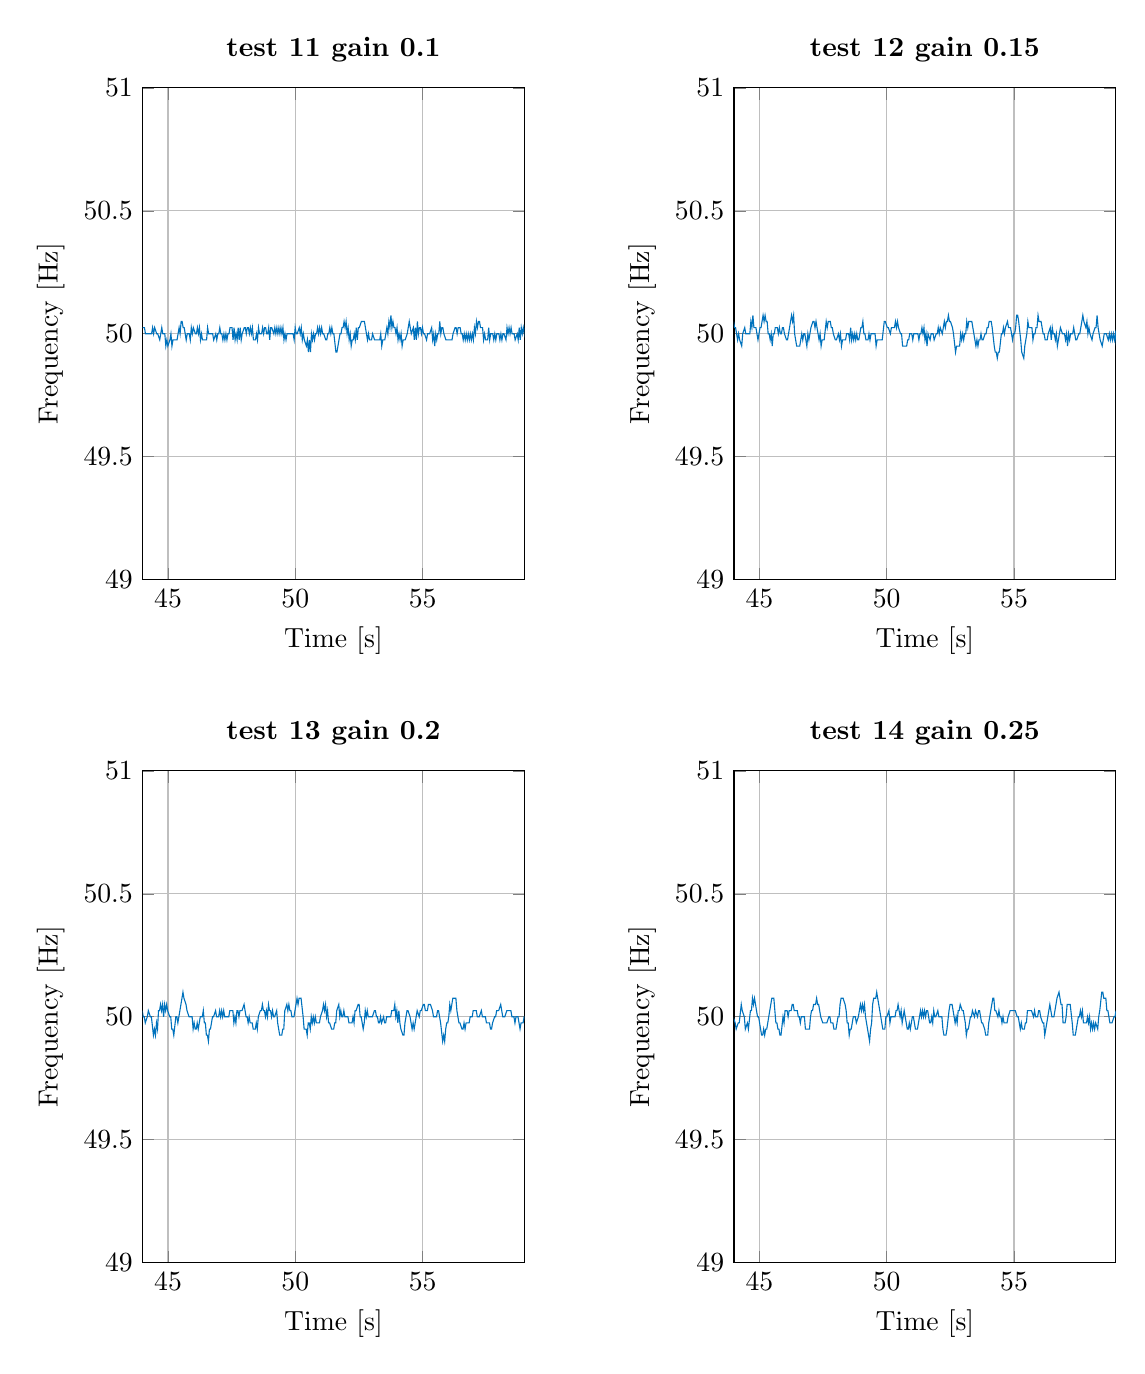
\begin{tikzpicture}

\begin{axis}[%
width=0.4\textwidth,
height=2.459in,
at={(1.043in,4.208in)},
scale only axis,
xmin=44,
xmax=59,
xlabel={Time [s]},
xmajorgrids,
ymin=49,
ymax=51,
ylabel={Frequency [Hz]},
ymajorgrids,
axis background/.style={fill=white},
title style={font=\bfseries},
title={test 11 gain 0.1}
]
\addplot [color=mycolor1,solid,forget plot]
  table[row sep=crcr]{%
43.99492	50.0250125062532\\
44.07488	50.0250125062532\\
44.11486	49.9999999999922\\
44.15486	50.0000000000011\\
44.19486	50.0000000000011\\
44.23486	50.0000000000011\\
44.31486	50.0000000000011\\
44.35486	50.0000000000011\\
44.39486	50.0250125062532\\
44.43484	50.0000000000011\\
44.47484	50.0250125062532\\
44.5548	49.9999999999922\\
44.5948	50.0000000000011\\
44.6748	49.9750124937551\\
44.71482	50.0000000000011\\
44.75482	50.0250125062532\\
44.7948	50.0000000000011\\
44.8348	50.0000000000011\\
44.8748	49.9999999999922\\
44.9148	49.9500499500529\\
44.95484	49.9750124937551\\
44.99486	49.9500499500529\\
45.07492	49.9750124937551\\
45.11494	50.0000000000011\\
45.15494	49.9500499500529\\
45.19498	49.9750124937463\\
45.235	49.9750124937551\\
45.31504	49.9750124937551\\
45.35506	49.9750124937551\\
45.39508	49.9999999999922\\
45.43508	50.0250125062532\\
45.47506	50.0000000000011\\
45.51506	50.0500500500492\\
45.55502	50.0500500500581\\
45.59498	50.0250125062444\\
45.63496	50.0250125062532\\
45.71492	49.9750124937551\\
45.75494	50.0000000000011\\
45.83494	50.0000000000011\\
45.87494	49.9750124937551\\
45.91496	50.0250125062532\\
45.95494	50.0000000000011\\
45.99494	50.0250125062532\\
46.0749	49.9999999999922\\
46.1149	50.0000000000011\\
46.1549	50.0250125062532\\
46.19488	50.0000000000011\\
46.23488	50.0250125062532\\
46.27486	49.9750124937551\\
46.31488	50.0000000000011\\
46.35488	49.9750124937551\\
46.3949	49.9750124937463\\
46.43492	49.9750124937551\\
46.47494	49.9750124937551\\
46.51496	49.9750124937551\\
46.55498	50.0250125062532\\
46.59496	50.0000000000011\\
46.63496	49.9999999999922\\
46.67496	50.0000000000011\\
46.71496	50.0000000000011\\
46.75496	50.0000000000011\\
46.79496	49.9750124937551\\
46.875	49.9999999999922\\
46.915	49.9750124937551\\
46.95502	50.0000000000011\\
46.99502	50.0000000000011\\
47.03502	50.0250125062532\\
47.075	50.0000000000011\\
47.115	50.0000000000011\\
47.155	49.9750124937551\\
47.19502	49.9999999999922\\
47.23502	49.9750124937551\\
47.27504	50.0000000000011\\
47.31504	49.9750124937551\\
47.35506	50.0000000000011\\
47.39506	50.0000000000011\\
47.43506	50.0250125062532\\
47.51502	50.0250125062532\\
47.555	49.9750124937463\\
47.59502	50.0250125062532\\
47.635	49.9750124937551\\
47.67502	50.0000000000011\\
47.71502	49.9750124937551\\
47.75504	50.0250125062532\\
47.79502	49.9750124937463\\
47.83504	50.0250125062532\\
47.87502	49.9750124937551\\
47.91504	50.0000000000011\\
47.99504	50.0250125062532\\
48.03502	50.0250125062532\\
48.075	50.0000000000011\\
48.115	50.0250125062532\\
48.15498	50.0250125062532\\
48.19496	50.0000000000011\\
48.23496	50.0250125062532\\
48.27494	50.0000000000011\\
48.31494	50.0250125062532\\
48.35492	49.9750124937463\\
48.39494	49.9750124937551\\
48.43496	49.9750124937551\\
48.47498	50.0000000000011\\
48.51498	49.9750124937551\\
48.555	50.0250125062532\\
48.59498	49.9999999999922\\
48.63498	50.0000000000011\\
48.67498	50.0000000000011\\
48.71498	50.0250125062532\\
48.75496	50.0000000000011\\
48.79496	50.0250125062532\\
48.83494	50.0250125062532\\
48.87492	50.0000000000011\\
48.91492	50.0000000000011\\
48.95492	50.0250125062532\\
48.9949	49.9750124937551\\
49.03492	50.0250125062532\\
49.0749	50.0250125062532\\
49.15486	49.9999999999922\\
49.19486	50.0250125062532\\
49.23484	50.0000000000011\\
49.27484	50.0250125062532\\
49.31482	50.0000000000011\\
49.35482	50.0250125062532\\
49.3948	50.0000000000011\\
49.4348	50.0250125062532\\
49.47478	50.0000000000011\\
49.51478	50.0250125062532\\
49.55476	49.9750124937551\\
49.59478	50.0000000000011\\
49.63478	49.9750124937463\\
49.6748	50.0000000000011\\
49.7148	50.0000000000011\\
49.7948	50.0000000000011\\
49.8348	50.0000000000011\\
49.9148	49.9999999999922\\
49.9548	49.9750124937551\\
49.99482	50.0250125062532\\
50.0348	50.0000000000011\\
50.0748	50.0000000000011\\
50.1548	50.0250125062532\\
50.19478	50.0000000000011\\
50.23478	50.0250125062532\\
50.27476	49.9750124937463\\
50.31478	50.0000000000011\\
50.35478	49.9750124937551\\
50.43482	49.9500499500529\\
50.47486	49.9750124937463\\
50.51488	49.9251123315066\\
50.55494	49.9750124937551\\
50.59496	49.9251123314978\\
50.63502	50.0000000000011\\
50.67502	49.9750124937551\\
50.71504	50.0000000000011\\
50.75504	49.9750124937551\\
50.79506	49.9999999999922\\
50.83506	50.0000000000011\\
50.87506	50.0250125062532\\
50.91504	50.0000000000011\\
50.95504	50.0250125062532\\
50.99502	50.0000000000011\\
51.03502	50.0250125062532\\
51.075	50.0000000000011\\
51.115	50.0000000000011\\
51.19502	49.9750124937463\\
51.23504	49.9750124937551\\
51.27506	50.0000000000011\\
51.31506	50.0000000000011\\
51.35506	50.0250125062532\\
51.39504	50.0000000000011\\
51.43504	50.0250125062532\\
51.47502	50.0000000000011\\
51.51502	49.9999999999922\\
51.59506	49.9251123315066\\
51.63512	49.9251123314978\\
51.71522	49.9750124937551\\
51.75524	50.0000000000011\\
51.79524	49.9999999999922\\
51.83524	50.0250125062532\\
51.87522	50.0250125062532\\
51.9152	50.0500500500581\\
51.95516	50.0250125062532\\
51.99514	50.0500500500492\\
52.0351	50.0000000000011\\
52.0751	50.0250125062444\\
52.11508	49.9750124937551\\
52.1551	50.0000000000011\\
52.1951	49.9500499500529\\
52.23514	49.9750124937551\\
52.27516	49.9750124937463\\
52.31518	50.0000000000011\\
52.35518	49.9750124937551\\
52.3952	50.0250125062532\\
52.43518	49.9750124937551\\
52.4752	50.0250125062532\\
52.51518	50.0250125062532\\
52.59514	50.0500500500492\\
52.6351	50.0500500500492\\
52.71502	50.0500500500492\\
52.75498	50.0250125062532\\
52.83494	49.9750124937551\\
52.87496	50.0000000000011\\
52.91496	49.9750124937551\\
52.95498	49.9750124937463\\
52.995	49.9750124937551\\
53.03502	50.0000000000011\\
53.11504	49.9750124937463\\
53.15506	49.9750124937551\\
53.2351	49.9750124937551\\
53.31514	49.9750124937463\\
53.35516	50.0000000000011\\
53.39516	49.9500499500529\\
53.4352	49.9750124937551\\
53.47522	49.9750124937463\\
53.51524	49.9750124937551\\
53.59528	50.0250125062532\\
53.63526	50.0000000000011\\
53.67526	50.0500500500492\\
53.71522	50.0250125062532\\
53.7552	50.0751126690017\\
53.79514	50.0250125062532\\
53.83512	50.0500500500492\\
53.87508	50.0250125062532\\
53.91506	50.0250125062532\\
53.95504	50.0000000000011\\
53.99504	50.0250125062532\\
54.03502	49.9750124937551\\
54.07504	50.0000000000011\\
54.11504	49.9750124937551\\
54.15506	49.9999999999922\\
54.19506	49.9500499500529\\
54.2351	49.9750124937551\\
54.27512	49.9750124937551\\
54.31514	49.9750124937463\\
54.39518	50.0000000000011\\
54.43518	50.0250125062532\\
54.47516	50.0500500500492\\
54.51512	50.0250125062532\\
54.5551	50.0000000000011\\
54.6351	50.0250125062532\\
54.67508	49.9750124937551\\
54.7151	50.0250125062532\\
54.75508	49.9750124937463\\
54.7951	50.0500500500492\\
54.83506	50.0000000000011\\
54.87506	50.0250125062532\\
54.91504	50.0250125062532\\
54.95502	50.0000000000011\\
54.99502	50.0250125062532\\
55.035	50.0000000000011\\
55.075	50.0000000000011\\
55.155	49.9750124937551\\
55.19502	49.9999999999922\\
55.23502	50.0000000000011\\
55.27502	50.0000000000011\\
55.35502	50.0250125062532\\
55.395	49.9750124937551\\
55.43502	50.0000000000011\\
55.47502	49.950049950044\\
55.51506	50.0000000000011\\
55.55506	49.9750124937551\\
55.59508	50.0000000000011\\
55.63508	50.0000000000011\\
55.67508	50.0500500500492\\
55.71504	50.0000000000011\\
55.75504	50.0250125062532\\
55.79502	50.0250125062532\\
55.835	50.0000000000011\\
55.915	49.9750124937463\\
55.95502	49.9750124937551\\
56.03506	49.9750124937551\\
56.07508	49.9750124937463\\
56.1151	49.9750124937551\\
56.15512	49.9750124937551\\
56.19514	50.0000000000011\\
56.27514	50.0250125062532\\
56.31512	50.0250125062532\\
56.3551	50.0000000000011\\
56.3951	50.0250125062532\\
56.43508	50.0250125062532\\
56.47506	50.0250125062532\\
56.51504	49.9999999999922\\
56.55504	50.0000000000011\\
56.59504	49.9750124937551\\
56.63506	50.0000000000011\\
56.67506	49.9750124937551\\
56.71508	50.0000000000011\\
56.75508	49.9750124937463\\
56.7951	50.0000000000011\\
56.8351	49.9750124937551\\
56.87512	50.0000000000011\\
56.91512	49.9750124937551\\
56.95514	50.0000000000011\\
56.99514	49.9750124937463\\
57.03516	50.0250125062532\\
57.07514	50.0000000000011\\
57.11514	50.0500500500492\\
57.1551	50.0250125062532\\
57.19508	50.0500500500492\\
57.23504	50.0500500500581\\
57.275	50.0250125062444\\
57.31498	50.0250125062532\\
57.35496	50.0250125062532\\
57.39494	49.9750124937551\\
57.43496	50.0000000000011\\
57.47496	49.9750124937551\\
57.555	49.9750124937463\\
57.59502	50.0250125062532\\
57.635	49.9750124937551\\
57.67502	50.0000000000011\\
57.71502	50.0000000000011\\
57.75502	50.0000000000011\\
57.79502	49.9750124937551\\
57.83504	50.0000000000011\\
57.87504	49.9750124937463\\
57.91506	50.0000000000011\\
57.95506	50.0000000000011\\
57.99506	50.0000000000011\\
58.03506	49.9750124937551\\
58.07508	50.0000000000011\\
58.11508	49.9750124937463\\
58.1551	50.0000000000011\\
58.1951	50.0000000000011\\
58.2751	49.9750124937551\\
58.31512	50.0250125062532\\
58.3551	50.0000000000011\\
58.3951	50.0250125062532\\
58.43508	49.9999999999922\\
58.47508	50.0250125062532\\
58.51506	50.0000000000011\\
58.59506	50.0000000000011\\
58.63506	49.9750124937551\\
58.7151	50.0000000000011\\
58.7551	49.9750124937463\\
58.79512	50.0250125062532\\
58.8351	49.9750124937551\\
58.87512	50.0250125062532\\
58.9151	50.0000000000011\\
58.9551	50.0250125062532\\
58.99508	50.0000000000011\\
59.03508	50.0500500500492\\
};
\end{axis}

\begin{axis}[%
width=0.4\textwidth,
height=2.459in,
at={(4in,4.208in)},
scale only axis,
xmin=44,
xmax=59,
xlabel={Time [s]},
xmajorgrids,
ymin=49,
ymax=51,
ylabel={Frequency [Hz]},
ymajorgrids,
axis background/.style={fill=white},
title style={font=\bfseries},
title={test 12  gain 0.15}
]
\addplot [color=mycolor1,solid,forget plot]
  table[row sep=crcr]{%
43.98424	50.0500500500492\\
44.0242	50.0250125062532\\
44.06418	50.0250125062532\\
44.10416	49.9999999999922\\
44.14416	49.9750124937551\\
44.18418	50.0000000000011\\
44.22418	49.9750124937551\\
44.30422	49.950049950044\\
44.34426	50.0000000000011\\
44.42426	50.0250125062532\\
44.46424	50.0000000000011\\
44.54424	50.0000000000011\\
44.62424	49.9999999999922\\
44.66424	50.0500500500581\\
44.7042	50.0250125062532\\
44.74418	50.0751126690017\\
44.78412	50.0250125062532\\
44.8241	50.0250125062532\\
44.86408	50.0250125062532\\
44.94406	49.9750124937463\\
44.98408	50.0000000000011\\
45.02408	50.0250125062532\\
45.06406	50.0250125062532\\
45.10404	50.0500500500492\\
45.144	50.0751126690106\\
45.18394	50.0500500500492\\
45.2239	50.0751126690017\\
45.26384	50.0500500500492\\
45.3038	50.0500500500492\\
45.34376	50.0000000000011\\
45.38376	50.0000000000011\\
45.42376	49.9750124937551\\
45.46378	49.9999999999922\\
45.50378	49.9500499500529\\
45.54382	50.0000000000011\\
45.58382	50.0000000000011\\
45.62382	50.0250125062532\\
45.70378	50.0250125062532\\
45.74376	50.0000000000011\\
45.78376	50.0250125062532\\
45.82374	50.0000000000011\\
45.86374	49.9999999999922\\
45.90374	50.0250125062532\\
45.94372	50.0250125062532\\
45.9837	50.0000000000011\\
46.0637	49.9750124937551\\
46.10372	49.9750124937551\\
46.14374	50.0000000000011\\
46.22372	50.0500500500492\\
46.26368	50.0751126690017\\
46.30362	50.0500500500492\\
46.34358	50.0751126690017\\
46.38352	50.0000000000011\\
46.46352	49.9500499500529\\
46.50356	49.950049950044\\
46.5436	49.9500499500529\\
46.58364	49.9500499500529\\
46.62368	49.9750124937463\\
46.6637	50.0000000000011\\
46.7037	49.9750124937551\\
46.74372	50.0000000000011\\
46.78372	50.0000000000011\\
46.86372	49.950049950044\\
46.90376	50.0000000000011\\
46.94376	49.9750124937551\\
46.98378	50.0000000000011\\
47.02378	50.0250125062532\\
47.10374	50.0500500500492\\
47.1437	50.0500500500492\\
47.18366	50.0250125062532\\
47.22364	50.0500500500492\\
47.2636	50.0250125062532\\
47.34358	49.9750124937551\\
47.3836	50.0000000000011\\
47.4236	49.950049950044\\
47.46364	49.9750124937551\\
47.50366	49.9750124937551\\
47.54368	49.9750124937551\\
47.6237	50.0500500500492\\
47.66366	50.0250125062532\\
47.70364	50.0500500500492\\
47.7436	50.0500500500492\\
47.78356	50.0500500500492\\
47.82352	50.0250125062532\\
47.8635	50.0250125062532\\
47.90348	50.0000000000011\\
47.98348	49.9750124937463\\
48.0235	49.9750124937551\\
48.10354	50.0000000000011\\
48.14354	49.9750124937551\\
48.18356	49.9999999999922\\
48.22356	49.9500499500529\\
48.2636	49.9750124937551\\
48.30362	49.9750124937551\\
48.34364	49.9750124937463\\
48.38366	49.9750124937551\\
48.42368	50.0000000000011\\
48.50368	50.0000000000011\\
48.54368	49.9750124937551\\
48.5837	50.0250125062532\\
48.62368	49.9750124937463\\
48.6637	50.0000000000011\\
48.7037	49.9750124937551\\
48.74372	50.0000000000011\\
48.78372	49.9750124937551\\
48.82374	50.0000000000011\\
48.86374	49.9750124937463\\
48.90376	49.9750124937551\\
48.94378	50.0000000000011\\
48.98378	50.0250125062532\\
49.02376	50.0250125062532\\
49.06374	50.0500500500492\\
49.1037	50.0000000000011\\
49.1437	50.0000000000011\\
49.1837	49.9750124937551\\
49.22372	49.9750124937463\\
49.26374	49.9750124937551\\
49.30376	50.0000000000011\\
49.34376	49.9750124937551\\
49.38378	50.0000000000011\\
49.42378	50.0000000000011\\
49.46378	49.9999999999922\\
49.50378	50.0000000000011\\
49.54378	50.0000000000011\\
49.58378	49.9500499500529\\
49.62382	49.9750124937551\\
49.66384	49.9750124937463\\
49.70386	49.9750124937551\\
49.7839	49.9750124937551\\
49.82392	49.9750124937551\\
49.90392	50.0500500500492\\
49.94388	50.0500500500492\\
50.0238	50.0250125062532\\
50.06378	50.0250125062532\\
50.14374	50.0000000000011\\
50.18374	50.0250125062532\\
50.22372	50.0250125062532\\
50.30368	50.0250125062532\\
50.34366	50.0500500500492\\
50.38362	50.0250125062532\\
50.4236	50.0500500500492\\
50.46356	50.0250125062532\\
50.54352	50.0000000000011\\
50.58352	50.0000000000011\\
50.62352	49.950049950044\\
50.66356	49.9500499500529\\
50.7036	49.9500499500529\\
50.74364	49.950049950044\\
50.78368	49.9500499500529\\
50.82372	49.9750124937551\\
50.86374	49.9750124937463\\
50.90376	50.0000000000011\\
50.94376	50.0000000000011\\
50.98376	50.0000000000011\\
51.02376	49.9750124937551\\
51.06378	50.0000000000011\\
51.10378	50.0000000000011\\
51.14378	49.9999999999922\\
51.18378	50.0000000000011\\
51.22378	50.0000000000011\\
51.26378	49.9750124937551\\
51.3038	50.0000000000011\\
51.3438	50.0000000000011\\
51.3838	50.0250125062532\\
51.42378	50.0000000000011\\
51.46378	50.0250125062532\\
51.50376	49.9750124937463\\
51.54378	50.0000000000011\\
51.58378	49.9500499500529\\
51.62382	50.0000000000011\\
51.70384	49.9750124937463\\
51.74386	50.0000000000011\\
51.82386	50.0000000000011\\
51.86386	49.9750124937551\\
51.9439	49.9999999999922\\
51.9839	50.0000000000011\\
52.0239	50.0250125062532\\
52.06388	50.0000000000011\\
52.10388	50.0250125062532\\
52.18384	50.0000000000011\\
52.22384	50.0250125062532\\
52.26382	50.0500500500492\\
52.30378	50.0250125062532\\
52.34376	50.0500500500492\\
52.38372	50.0500500500492\\
52.42368	50.0751126690017\\
52.46362	50.0500500500581\\
52.50358	50.0500500500492\\
52.5835	50.0250125062532\\
52.62348	50.0000000000011\\
52.7035	49.9251123315066\\
52.74356	49.9500499500529\\
52.7836	49.950049950044\\
52.82364	49.9500499500529\\
52.86368	49.9500499500529\\
52.90372	50.0000000000011\\
52.94372	49.9750124937463\\
52.98374	50.0000000000011\\
53.02374	49.9750124937551\\
53.06376	50.0000000000011\\
53.10376	50.0000000000011\\
53.14376	50.0500500500492\\
53.18372	50.0250125062532\\
53.2237	50.0500500500492\\
53.26366	50.0500500500492\\
53.34358	50.0500500500492\\
53.38354	50.0250125062532\\
53.46352	49.9750124937551\\
53.50354	49.950049950044\\
53.54358	49.9750124937551\\
53.5836	49.9500499500529\\
53.62364	49.9750124937551\\
53.66366	49.9750124937463\\
53.70368	50.0000000000011\\
53.74368	49.9750124937551\\
53.7837	49.9750124937551\\
53.86374	50.0000000000011\\
53.90374	49.9999999999922\\
53.94374	50.0250125062532\\
53.98372	50.0250125062532\\
54.0237	50.0500500500492\\
54.06366	50.0500500500581\\
54.10362	50.0500500500492\\
54.14358	50.0250125062532\\
54.22356	49.950049950044\\
54.2636	49.9251123315066\\
54.30366	49.9251123314978\\
54.34372	49.9001996008032\\
54.3838	49.9251123314978\\
54.42386	49.9251123315066\\
54.50396	49.9999999999922\\
54.54396	50.0000000000011\\
54.58396	50.0250125062532\\
54.62394	50.0000000000011\\
54.66394	50.0250125062532\\
54.7439	50.0500500500492\\
54.78386	50.0250125062532\\
54.86382	50.0250125062532\\
54.9038	50.0000000000011\\
54.9438	49.9750124937551\\
54.98382	50.0000000000011\\
55.02382	50.0000000000011\\
55.06382	50.0250125062532\\
55.1038	50.0751126690017\\
55.14374	50.0751126690017\\
55.18368	50.0500500500492\\
55.2636	49.9750124937551\\
55.30362	49.9251123315066\\
55.38374	49.9001996008032\\
55.42382	49.950049950044\\
55.50388	50.0000000000011\\
55.54388	50.0500500500492\\
55.58384	50.0250125062532\\
55.62382	50.0250125062532\\
55.6638	50.0250125062532\\
55.70378	50.0250125062532\\
55.74376	49.9750124937551\\
55.78378	50.0000000000011\\
55.82378	49.9999999999922\\
55.86378	50.0250125062532\\
55.90376	50.0250125062532\\
55.94374	50.0751126690106\\
55.98368	50.0500500500492\\
56.02364	50.0500500500492\\
56.0636	50.0500500500492\\
56.14354	50.0000000000011\\
56.18354	50.0000000000011\\
56.22354	49.9750124937463\\
56.26356	49.9750124937551\\
56.30358	49.9750124937551\\
56.3436	50.0000000000011\\
56.4236	50.0250125062532\\
56.46358	49.9750124937551\\
56.5036	50.0250125062532\\
56.54358	49.9999999999922\\
56.58358	50.0000000000011\\
56.62358	49.9750124937551\\
56.6636	50.0000000000011\\
56.7036	49.9500499500529\\
56.78364	50.0000000000011\\
56.82364	50.0250125062532\\
56.9036	50.0000000000011\\
56.9436	50.0000000000011\\
56.9836	50.0000000000011\\
57.0236	49.9750124937551\\
57.06362	50.0000000000011\\
57.10362	49.950049950044\\
57.14366	50.0000000000011\\
57.18366	49.9750124937551\\
57.22368	50.0000000000011\\
57.30368	50.0000000000011\\
57.34368	50.0250125062532\\
57.42366	49.9750124937551\\
57.46368	49.9750124937551\\
57.54372	50.0000000000011\\
57.58372	50.0000000000011\\
57.6637	50.0500500500492\\
57.70366	50.0751126690017\\
57.7436	50.0500500500492\\
57.82352	50.0250125062532\\
57.8635	50.0500500500492\\
57.90346	50.0000000000011\\
57.94346	50.0250125062532\\
57.98344	50.0000000000011\\
58.06346	49.9750124937463\\
58.10348	50.0000000000011\\
58.18348	50.0250125062532\\
58.22346	50.0250125062532\\
58.26344	50.0751126690017\\
58.30338	50.0250125062532\\
58.34336	50.0000000000011\\
58.38336	49.9750124937551\\
58.46342	49.950049950044\\
58.50346	49.9750124937551\\
58.54348	50.0000000000011\\
58.58348	50.0000000000011\\
58.62348	50.0000000000011\\
58.70348	49.9750124937463\\
58.7435	50.0000000000011\\
58.7835	49.9750124937551\\
58.82352	50.0000000000011\\
58.86352	49.9750124937551\\
58.90354	50.0000000000011\\
58.94354	49.9750124937463\\
58.98356	50.0000000000011\\
59.02356	49.9500499500529\\
};
\end{axis}

\begin{axis}[%
width=0.4\textwidth,
height=2.459in,
at={(1.043in,0.793in)},
scale only axis,
xmin=44,
xmax=59,
xlabel={Time [s]},
xmajorgrids,
ymin=49,
ymax=51,
ylabel={Frequency [Hz]},
ymajorgrids,
axis background/.style={fill=white},
title style={font=\bfseries},
title={test 13  gain 0.2}
]
\addplot [color=mycolor1,solid,forget plot]
  table[row sep=crcr]{%
43.98716	50.0250125062532\\
44.02714	50.0000000000011\\
44.06714	50.0000000000011\\
44.10714	49.9750124937463\\
44.18718	50.0000000000011\\
44.22718	50.0250125062532\\
44.30714	50.0000000000011\\
44.34714	50.0000000000011\\
44.42716	49.9251123314978\\
44.46722	49.9500499500529\\
44.50726	49.9251123314978\\
44.54732	49.9750124937551\\
44.58734	49.9500499500529\\
44.62738	50.0250125062532\\
44.66736	50.0250125062532\\
44.70734	50.0500500500492\\
44.7473	50.0250125062532\\
44.78728	50.0500500500492\\
44.82724	50.0000000000011\\
44.86724	50.0500500500492\\
44.9072	50.0250125062532\\
44.94718	50.0500500500492\\
44.98714	50.0250125062532\\
45.0671	50.0000000000011\\
45.1071	50.0000000000011\\
45.1471	49.950049950044\\
45.18714	49.9500499500529\\
45.22718	49.9251123315066\\
45.30726	50.0000000000011\\
45.34726	50.0000000000011\\
45.38726	49.9750124937551\\
45.46728	50.0250125062532\\
45.50726	50.0500500500492\\
45.58718	50.1002004007989\\
45.6271	50.0751126690106\\
45.70698	50.0500500500492\\
45.74694	50.0250125062532\\
45.8269	50.0000000000011\\
45.8669	50.0000000000011\\
45.9069	49.9999999999922\\
45.9469	50.0000000000011\\
45.9869	49.9500499500529\\
46.02694	49.9750124937551\\
46.06696	49.950049950044\\
46.107	49.9500499500529\\
46.14704	49.9750124937551\\
46.18706	49.9500499500529\\
46.2271	49.9750124937463\\
46.26712	50.0000000000011\\
46.34712	50.0000000000011\\
46.38712	50.0250125062532\\
46.4271	49.9750124937551\\
46.46712	49.9750124937551\\
46.50714	49.9251123314978\\
46.5472	49.9251123315066\\
46.58726	49.9001996007944\\
46.62734	49.9500499500529\\
46.66738	49.950049950044\\
46.70742	49.9750124937551\\
46.74744	50.0000000000011\\
46.78744	50.0000000000011\\
46.86744	50.0250125062532\\
46.90742	50.0000000000011\\
46.98742	49.9999999999922\\
47.02742	50.0250125062532\\
47.0674	50.0000000000011\\
47.1074	50.0250125062532\\
47.14738	50.0000000000011\\
47.18738	50.0250125062532\\
47.22736	50.0000000000011\\
47.26736	50.0000000000011\\
47.34736	50.0000000000011\\
47.38736	50.0000000000011\\
47.42736	50.0250125062532\\
47.50732	50.0250125062532\\
47.5473	50.0250125062532\\
47.58728	49.9750124937463\\
47.6273	50.0000000000011\\
47.6673	49.9750124937551\\
47.70732	50.0250125062532\\
47.7473	50.0250125062532\\
47.78728	50.0000000000011\\
47.82728	50.0250125062532\\
47.86726	50.0250125062532\\
47.90724	50.0250125062532\\
47.9872	50.0500500500492\\
48.02716	50.0250125062532\\
48.06714	50.0000000000011\\
48.10714	50.0000000000011\\
48.14714	49.9750124937463\\
48.18716	50.0000000000011\\
48.22716	49.9750124937551\\
48.26718	49.9750124937551\\
48.3072	49.9750124937551\\
48.34722	49.950049950044\\
48.38726	49.9500499500529\\
48.4273	49.9500499500529\\
48.46734	49.9750124937463\\
48.50736	49.9500499500529\\
48.5474	50.0000000000011\\
48.6274	50.0250125062532\\
48.66738	50.0250125062532\\
48.70736	50.0500500500492\\
48.74732	50.0250125062532\\
48.7873	50.0250125062532\\
48.82728	50.0000000000011\\
48.86728	50.0250125062532\\
48.90726	50.0000000000011\\
48.94726	50.0500500500492\\
48.98722	50.0250125062532\\
49.0272	50.0250125062532\\
49.06718	50.0000000000011\\
49.10718	50.0250125062532\\
49.14716	49.9999999999922\\
49.18716	50.0000000000011\\
49.26716	50.0250125062532\\
49.30714	49.9750124937551\\
49.3872	49.9251123314978\\
49.42726	49.9251123315066\\
49.46732	49.9251123314978\\
49.50738	49.9500499500529\\
49.54742	49.9500499500529\\
49.58746	50.0250125062532\\
49.66742	50.0500500500492\\
49.70738	50.0250125062532\\
49.74736	50.0500500500492\\
49.78732	50.0250125062532\\
49.8273	50.0250125062532\\
49.86728	50.0000000000011\\
49.90728	50.0000000000011\\
49.94728	49.9999999999922\\
50.02726	50.0500500500492\\
50.06722	50.0751126690106\\
50.10716	50.0500500500492\\
50.14712	50.0751126690017\\
50.18706	50.0751126690017\\
50.227	50.0751126690017\\
50.30692	50.0000000000011\\
50.34692	49.9500499500529\\
50.427	49.950049950044\\
50.46704	49.9251123315066\\
50.5071	49.9750124937551\\
50.54712	49.9750124937463\\
50.58714	49.9500499500529\\
50.62718	50.0000000000011\\
50.66718	49.9750124937551\\
50.7072	50.0000000000011\\
50.7472	49.9750124937463\\
50.78722	50.0000000000011\\
50.82722	49.9750124937551\\
50.86724	49.9750124937551\\
50.94728	49.9750124937463\\
50.9873	50.0000000000011\\
51.0673	50.0250125062532\\
51.10728	50.0500500500492\\
51.14724	50.0250125062532\\
51.18722	50.0500500500492\\
51.22718	50.0000000000011\\
51.26718	50.0250125062532\\
51.30716	49.9750124937551\\
51.34718	49.9750124937551\\
51.42722	49.9500499500529\\
51.46726	49.9500499500529\\
51.5073	49.950049950044\\
51.54734	49.9750124937551\\
51.58736	49.9750124937551\\
51.62738	50.0250125062532\\
51.70734	50.0500500500492\\
51.7473	50.0000000000011\\
51.7873	50.0250125062532\\
51.82728	50.0000000000011\\
51.86728	50.0000000000011\\
51.90728	50.0250125062532\\
51.94726	50.0000000000011\\
51.98726	49.9999999999922\\
52.02726	50.0000000000011\\
52.06726	50.0000000000011\\
52.10726	49.9750124937551\\
52.1873	49.9750124937463\\
52.22732	49.9750124937551\\
52.26734	50.0000000000011\\
52.30734	49.9750124937551\\
52.34736	50.0250125062532\\
52.38734	50.0250125062532\\
52.4673	50.0500500500492\\
52.50726	50.0500500500492\\
52.54722	50.0000000000011\\
52.58722	50.0000000000011\\
52.62722	49.9750124937551\\
52.66724	49.950049950044\\
52.70728	49.9750124937551\\
52.7473	50.0250125062532\\
52.78728	50.0000000000011\\
52.82728	50.0250125062532\\
52.86726	50.0000000000011\\
52.90726	50.0000000000011\\
52.98726	49.9999999999922\\
53.02726	50.0000000000011\\
53.10726	50.0250125062532\\
53.14724	50.0250125062532\\
53.18722	50.0000000000011\\
53.22722	50.0000000000011\\
53.26722	49.9750124937551\\
53.30724	49.9750124937463\\
53.34726	50.0000000000011\\
53.38726	49.9750124937551\\
53.4673	50.0000000000011\\
53.5073	49.9750124937551\\
53.54732	49.9750124937463\\
53.58734	50.0000000000011\\
53.62734	50.0000000000011\\
53.66734	50.0000000000011\\
53.74734	50.0000000000011\\
53.78734	50.0250125062532\\
53.8673	50.0250125062532\\
53.90728	50.0500500500492\\
53.94724	50.0000000000011\\
53.98724	50.0250125062532\\
54.02722	49.9750124937463\\
54.06724	50.0250125062532\\
54.10722	49.9750124937551\\
54.14724	49.9500499500529\\
54.22732	49.9251123314978\\
54.26738	49.9251123315066\\
54.30744	49.9750124937463\\
54.38748	50.0250125062532\\
54.42746	50.0250125062532\\
54.50742	50.0000000000011\\
54.54742	49.9750124937551\\
54.58744	49.950049950044\\
54.62748	49.9750124937551\\
54.6675	49.9500499500529\\
54.74756	50.0000000000011\\
54.78756	50.0250125062532\\
54.86752	49.9999999999922\\
54.90752	50.0250125062532\\
54.9475	50.0250125062532\\
55.02746	50.0500500500492\\
55.06742	50.0500500500581\\
55.10738	50.0250125062532\\
55.14736	50.0250125062532\\
55.18734	50.0250125062532\\
55.22732	50.0500500500492\\
55.26728	50.0500500500492\\
55.30724	50.0500500500492\\
55.38716	50.0250125062532\\
55.42714	50.0000000000011\\
55.50714	50.0000000000011\\
55.54714	49.9999999999922\\
55.58714	50.0250125062532\\
55.62712	50.0250125062532\\
55.6671	50.0000000000011\\
55.7071	49.9750124937551\\
55.78714	49.9001996007944\\
55.82722	49.9251123315066\\
55.86728	49.9001996007944\\
55.90736	49.9500499500529\\
55.9474	49.9750124937551\\
55.98742	49.9750124937463\\
56.02744	50.0000000000011\\
56.06744	50.0500500500492\\
56.1074	50.0250125062532\\
56.14738	50.0500500500581\\
56.18734	50.0751126690017\\
56.26722	50.0751126690017\\
56.30716	50.0751126690017\\
56.3471	50.0250125062532\\
56.42706	49.9750124937551\\
56.46708	49.9750124937551\\
56.54714	49.950049950044\\
56.58718	49.9500499500529\\
56.62722	49.9750124937551\\
56.66724	49.950049950044\\
56.70728	49.9750124937551\\
56.78732	49.9750124937551\\
56.82734	49.9750124937463\\
56.86736	50.0000000000011\\
56.90736	50.0000000000011\\
56.94736	50.0000000000011\\
56.98736	50.0250125062532\\
57.06732	50.0250125062532\\
57.1073	50.0250125062532\\
57.14728	50.0000000000011\\
57.18728	50.0000000000011\\
57.22728	50.0000000000011\\
57.30728	50.0250125062532\\
57.34726	49.9999999999922\\
57.38726	50.0000000000011\\
57.42726	50.0000000000011\\
57.46726	50.0000000000011\\
57.50726	49.9750124937551\\
57.54728	49.9750124937551\\
57.5873	49.9750124937463\\
57.62732	49.9750124937551\\
57.66734	49.9500499500529\\
57.70738	49.950049950044\\
57.74742	49.9750124937551\\
57.82746	50.0000000000011\\
57.86746	50.0000000000011\\
57.90746	50.0250125062532\\
57.94744	50.0250125062532\\
57.98742	50.0250125062532\\
58.06738	50.0500500500492\\
58.10734	50.0250125062532\\
58.14732	50.0000000000011\\
58.18732	50.0000000000011\\
58.22732	49.9999999999922\\
58.30732	50.0250125062532\\
58.3473	50.0250125062532\\
58.38728	50.0250125062532\\
58.46724	50.0250125062532\\
58.50722	50.0000000000011\\
58.58722	50.0000000000011\\
58.62722	49.9750124937551\\
58.66724	50.0000000000011\\
58.70724	49.9999999999922\\
58.74724	50.0000000000011\\
58.82726	49.9500499500529\\
58.8673	49.9750124937551\\
58.90732	49.9750124937463\\
58.94734	49.9750124937551\\
58.98736	50.0000000000011\\
59.02736	50.0000000000011\\
};
\end{axis}

\begin{axis}[%
width=0.4\textwidth,
height=2.459in,
at={(4in,0.793in)},
scale only axis,
xmin=44,
xmax=59,
xlabel={Time [s]},
xmajorgrids,
ymin=49,
ymax=51,
ylabel={Frequency [Hz]},
ymajorgrids,
axis background/.style={fill=white},
title style={font=\bfseries},
title={test 14  gain 0.25}
]
\addplot [color=mycolor1,solid,forget plot]
  table[row sep=crcr]{%
43.96722	50.0000000000011\\
44.04722	49.9750124937551\\
44.08724	49.950049950044\\
44.16732	49.9750124937551\\
44.20734	49.9750124937551\\
44.28734	50.0500500500492\\
44.3273	50.0250125062532\\
44.40728	49.9999999999922\\
44.44728	49.9500499500529\\
44.52736	49.9750124937551\\
44.56738	49.950049950044\\
44.64742	50.0250125062532\\
44.6874	50.0250125062532\\
44.72738	50.0751126690017\\
44.76732	50.0500500500492\\
44.80728	50.0751126690106\\
44.84722	50.0500500500492\\
44.92714	50.0000000000011\\
44.96714	50.0000000000011\\
45.04714	49.9500499500529\\
45.08718	49.9251123315066\\
45.12724	49.9251123314978\\
45.1673	49.9500499500529\\
45.20734	49.9251123314978\\
45.2474	49.9500499500529\\
45.28744	49.9500499500529\\
45.32748	49.9750124937551\\
45.3675	49.9999999999922\\
45.44748	50.0500500500492\\
45.48744	50.0751126690106\\
45.52738	50.0751126690017\\
45.56732	50.0751126690017\\
45.60726	50.0250125062532\\
45.64724	49.9750124937551\\
45.68726	49.9750124937551\\
45.72728	49.950049950044\\
45.76732	49.9500499500529\\
45.80736	49.9251123315066\\
45.84742	49.9251123314978\\
45.92752	50.0000000000011\\
45.96752	49.9750124937463\\
46.00754	50.0250125062532\\
46.0875	50.0250125062532\\
46.12748	50.0000000000011\\
46.16748	50.0250125062532\\
46.20746	50.0250125062532\\
46.24744	50.0250125062532\\
46.28742	50.0500500500492\\
46.32738	50.0500500500492\\
46.36734	50.0250125062532\\
46.4473	50.0250125062532\\
46.48728	50.0250125062532\\
46.52726	50.0000000000011\\
46.56726	50.0000000000011\\
46.60726	49.9750124937551\\
46.64728	50.0000000000011\\
46.68728	50.0000000000011\\
46.72728	50.0000000000011\\
46.76728	49.9999999999922\\
46.80728	49.9500499500529\\
46.84732	49.9500499500529\\
46.88736	49.950049950044\\
46.9274	49.9500499500529\\
46.96744	49.9500499500529\\
47.00748	50.0000000000011\\
47.04748	50.0250125062532\\
47.08746	50.0250125062532\\
47.12744	50.0500500500492\\
47.20736	50.0500500500492\\
47.24732	50.0751126690017\\
47.28726	50.0500500500492\\
47.32722	50.0500500500492\\
47.36718	50.0250125062532\\
47.40716	50.0000000000011\\
47.48716	49.9750124937551\\
47.52718	49.9750124937551\\
47.5672	49.9750124937463\\
47.60722	49.9750124937551\\
47.64724	49.9750124937551\\
47.72728	50.0000000000011\\
47.76728	49.9999999999922\\
47.80728	49.9750124937551\\
47.8473	49.9750124937551\\
47.88732	49.9750124937551\\
47.92734	49.950049950044\\
47.96738	49.9500499500529\\
48.00742	49.9500499500529\\
48.08748	50.0000000000011\\
48.12748	50.0000000000011\\
48.16748	50.0500500500492\\
48.20744	50.0751126690106\\
48.24738	50.0751126690017\\
48.28732	50.0751126690017\\
48.3672	50.0500500500492\\
48.40716	50.0250125062532\\
48.44714	49.9750124937551\\
48.48716	49.9750124937551\\
48.52718	49.9251123314978\\
48.56724	49.9500499500529\\
48.60728	49.9500499500529\\
48.64732	49.9750124937463\\
48.68734	50.0000000000011\\
48.72734	50.0000000000011\\
48.76734	50.0000000000011\\
48.80734	49.9750124937551\\
48.88738	50.0000000000011\\
48.92738	50.0250125062532\\
48.96736	50.0500500500492\\
49.00732	50.0250125062532\\
49.0473	50.0500500500492\\
49.08726	50.0250125062532\\
49.12724	50.0500500500492\\
49.1672	50.0000000000011\\
49.24722	49.9500499500529\\
49.28726	49.9251123315066\\
49.32732	49.9001996007944\\
49.3674	49.9500499500529\\
49.40744	49.9750124937551\\
49.44746	50.0500500500492\\
49.48742	50.0751126690017\\
49.52736	50.0751126690017\\
49.5673	50.0751126690017\\
49.60724	50.1002004008078\\
49.64716	50.0751126690017\\
49.6871	50.0500500500492\\
49.76704	50.0000000000011\\
49.80704	49.9750124937463\\
49.84706	49.9500499500529\\
49.8871	49.9500499500529\\
49.92714	49.950049950044\\
49.96718	50.0000000000011\\
50.00718	50.0000000000011\\
50.08718	50.0250125062532\\
50.12716	49.9750124937551\\
50.16718	50.0000000000011\\
50.20718	50.0000000000011\\
50.28718	49.9999999999922\\
50.32718	50.0000000000011\\
50.36718	50.0250125062532\\
50.40716	50.0250125062532\\
50.44714	50.0500500500492\\
50.52708	50.0000000000011\\
50.56708	50.0250125062532\\
50.60706	49.9750124937551\\
50.64708	50.0000000000011\\
50.68708	50.0250125062532\\
50.76706	49.9750124937551\\
50.80708	49.950049950044\\
50.84712	49.9500499500529\\
50.88716	49.9750124937551\\
50.92718	49.950049950044\\
50.96722	49.9750124937551\\
51.00724	50.0000000000011\\
51.04724	50.0000000000011\\
51.08724	49.9750124937551\\
51.12726	49.950049950044\\
51.1673	49.9500499500529\\
51.20734	49.9500499500529\\
51.2874	50.0000000000011\\
51.3274	50.0250125062532\\
51.36738	50.0000000000011\\
51.40738	50.0250125062532\\
51.44736	50.0000000000011\\
51.48736	50.0250125062532\\
51.52734	50.0000000000011\\
51.56734	50.0250125062532\\
51.60732	50.0250125062532\\
51.6873	49.9750124937463\\
51.72732	49.9750124937551\\
51.76734	50.0000000000011\\
51.80734	49.9750124937551\\
51.84736	50.0250125062532\\
51.88734	50.0000000000011\\
51.92734	50.0000000000011\\
52.00734	50.0250125062532\\
52.04732	49.9999999999922\\
52.08732	50.0000000000011\\
52.16732	50.0000000000011\\
52.20732	49.9500499500529\\
52.24736	49.9251123314978\\
52.28742	49.9251123315066\\
52.32748	49.9251123314978\\
52.36754	49.9500499500529\\
52.44758	50.0250125062532\\
52.48756	50.0500500500492\\
52.56748	50.0500500500492\\
52.60744	50.0250125062532\\
52.6874	49.9750124937551\\
52.72742	50.0000000000011\\
52.76742	49.9750124937551\\
52.80744	50.0250125062532\\
52.84742	50.0250125062532\\
52.8874	50.0500500500492\\
52.96732	50.0250125062532\\
53.0073	50.0250125062532\\
53.08728	49.9750124937463\\
53.1273	49.9251123315066\\
53.16736	49.9500499500529\\
53.2074	49.950049950044\\
53.24744	49.9750124937551\\
53.28746	50.0000000000011\\
53.32746	50.0000000000011\\
53.36746	50.0250125062532\\
53.44742	50.0000000000011\\
53.48742	50.0250125062532\\
53.56738	50.0000000000011\\
53.60738	50.0250125062532\\
53.64736	50.0250125062532\\
53.72732	49.9750124937463\\
53.76734	49.9750124937551\\
53.8474	49.950049950044\\
53.88744	49.9251123315066\\
53.96756	49.9251123314978\\
54.00762	49.9750124937551\\
54.08764	50.0250125062532\\
54.12762	50.0500500500492\\
54.16758	50.0751126690017\\
54.20752	50.0751126690017\\
54.24746	50.0250125062532\\
54.28744	50.0250125062532\\
54.3674	50.0000000000011\\
54.4074	50.0250125062532\\
54.44738	50.0000000000011\\
54.48738	50.0000000000011\\
54.52738	49.9750124937551\\
54.5674	49.9999999999922\\
54.6074	49.9750124937551\\
54.64742	49.9750124937551\\
54.72746	49.9750124937551\\
54.76748	49.9999999999922\\
54.84748	50.0250125062532\\
54.88746	50.0250125062532\\
54.92744	50.0250125062532\\
55.0074	50.0250125062532\\
55.04738	50.0250125062532\\
55.12734	50.0000000000011\\
55.16734	50.0000000000011\\
55.24736	49.950049950044\\
55.2874	49.9750124937551\\
55.32742	49.9500499500529\\
55.36746	49.9500499500529\\
55.4075	49.950049950044\\
55.44754	49.9750124937551\\
55.48756	49.9750124937551\\
55.52758	50.0250125062532\\
55.60754	50.0250125062532\\
55.64752	50.0250125062532\\
55.6875	50.0250125062532\\
55.76746	50.0000000000011\\
55.80746	50.0250125062532\\
55.84744	49.9999999999922\\
55.88744	50.0000000000011\\
55.92744	50.0000000000011\\
55.96744	50.0250125062532\\
56.00742	50.0250125062532\\
56.0474	50.0000000000011\\
56.1274	49.9750124937551\\
56.16742	49.9750124937463\\
56.20744	49.9251123315066\\
56.2475	49.9500499500529\\
56.28754	49.9750124937463\\
56.32756	50.0000000000011\\
56.40756	50.0500500500492\\
56.44752	50.0250125062532\\
56.4875	50.0000000000011\\
56.5275	50.0000000000011\\
56.5675	50.0000000000011\\
56.6475	50.0500500500492\\
56.68746	50.0751126690017\\
56.76734	50.1002004008078\\
56.80726	50.0751126690017\\
56.8472	50.0500500500492\\
56.88716	50.0500500500492\\
56.92712	49.9750124937551\\
57.00716	49.9750124937463\\
57.04718	50.0000000000011\\
57.08718	50.0500500500492\\
57.1671	50.0500500500492\\
57.20706	50.0500500500581\\
57.287	49.9750124937463\\
57.32702	49.9251123315066\\
57.36708	49.9251123314978\\
57.40714	49.9251123315066\\
57.4472	49.9500499500529\\
57.52726	50.0000000000011\\
57.56726	50.0000000000011\\
57.60726	50.0250125062532\\
57.64724	50.0000000000011\\
57.68724	50.0250125062532\\
57.72722	49.9750124937551\\
57.80726	49.9750124937463\\
57.84728	49.9750124937551\\
57.8873	50.0000000000011\\
57.9273	49.9750124937551\\
57.96732	50.0000000000011\\
58.00732	49.950049950044\\
58.04736	49.9750124937551\\
58.08738	49.9500499500529\\
58.12742	49.9750124937551\\
58.16744	49.950049950044\\
58.20748	49.9750124937551\\
58.28752	49.950049950044\\
58.32756	50.0000000000011\\
58.36756	50.0250125062532\\
58.4475	50.1002004008078\\
58.48742	50.1002004007989\\
58.52734	50.0751126690017\\
58.56728	50.0751126690017\\
58.60722	50.0751126690106\\
58.64716	50.0250125062532\\
58.68714	50.0250125062532\\
58.72712	50.0000000000011\\
58.76712	49.9750124937463\\
58.80714	49.9750124937551\\
58.84716	49.9750124937551\\
58.9272	49.9999999999922\\
58.9672	50.0000000000011\\
59.0072	50.0250125062532\\
};
\end{axis}
\end{tikzpicture}%
\caption{Steady state at 30 kW load, with various scaling factors.}
\label{fig:test11-14steadyfrequency30kw}
\end{figure}

\begin{figure}[H]
\centering
% This file was created by matlab2tikz.
%
%The latest updates can be retrieved from
%  http://www.mathworks.com/matlabcentral/fileexchange/22022-matlab2tikz-matlab2tikz
%where you can also make suggestions and rate matlab2tikz.
%
\definecolor{mycolor1}{rgb}{0.00000,0.44700,0.74100}%
%
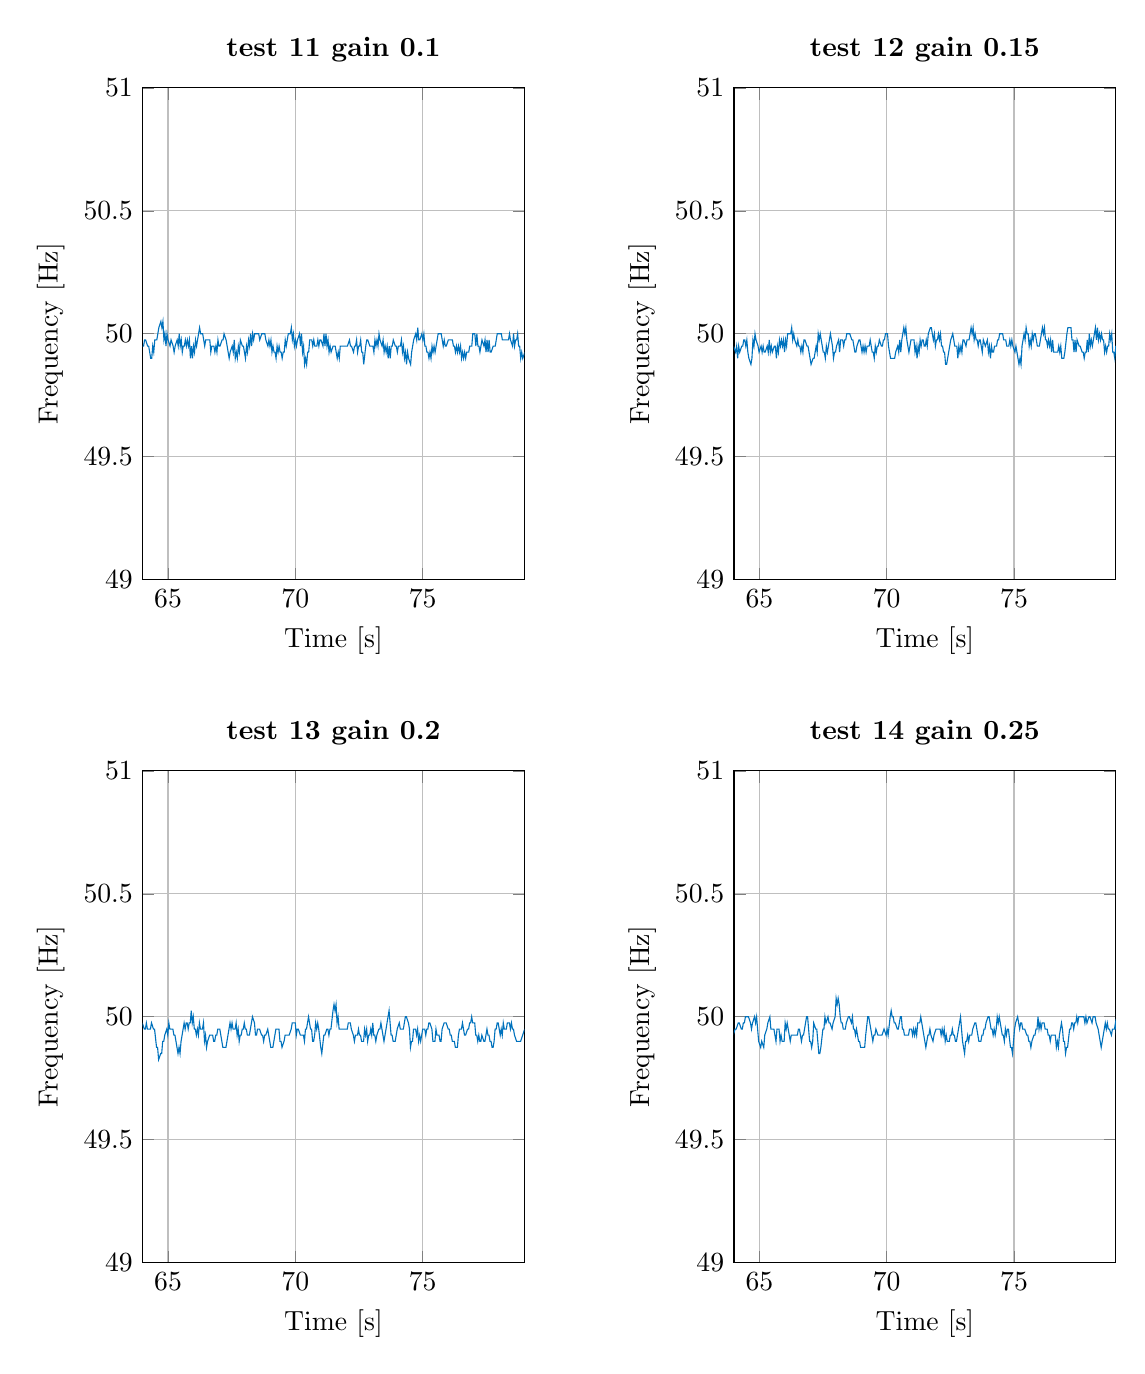
\begin{tikzpicture}

\begin{axis}[%
width=0.4\textwidth,
height=2.459in,
at={(1.043in,4.208in)},
scale only axis,
xmin=64,
xmax=79,
xlabel={Time [s]},
xmajorgrids,
ymin=49,
ymax=51,
ylabel={Frequency [Hz]},
ymajorgrids,
axis background/.style={fill=white},
title style={font=\bfseries},
title={test 11 gain 0.1}
]
\addplot [color=mycolor1,solid,forget plot]
  table[row sep=crcr]{%
63.9997	49.9500499500529\\
64.03974	49.950049950044\\
64.07978	49.9750124937551\\
64.1198	49.9750124937551\\
64.19984	49.950049950044\\
64.23988	49.9500499500618\\
64.31998	49.9001996008121\\
64.36006	49.9001996007944\\
64.40014	49.950049950044\\
64.44018	49.9251123315066\\
64.48024	49.9750124937551\\
64.56028	49.9750124937551\\
64.6003	49.9999999999922\\
64.6403	50.0250125062532\\
64.72026	50.0500500500581\\
64.76022	50.0250125062532\\
64.8002	50.0500500500403\\
64.84016	49.9750124937551\\
64.88018	50.0000000000099\\
64.92018	49.950049950044\\
64.96022	49.9999999999922\\
65.00022	49.9750124937551\\
65.08026	49.950049950044\\
65.1203	49.9750124937551\\
65.20036	49.950049950044\\
65.2404	49.9251123315066\\
65.28046	49.950049950044\\
65.36054	49.9750124937551\\
65.40056	49.9500499500618\\
65.4406	49.9999999999922\\
65.4806	49.950049950044\\
65.52064	49.9750124937551\\
65.56066	49.9251123315066\\
65.60072	49.950049950044\\
65.64076	49.9500499500618\\
65.6808	49.9750124937551\\
65.72082	49.950049950044\\
65.76086	49.9750124937551\\
65.80088	49.950049950044\\
65.84092	49.9750124937551\\
65.88094	49.9001996007944\\
65.92102	49.9500499500618\\
65.96106	49.9001996007944\\
66.00114	49.950049950044\\
66.04118	49.9251123315066\\
66.08124	49.9750124937551\\
66.12126	49.950049950044\\
66.1613	49.9750124937551\\
66.24134	50.0250125062532\\
66.28132	49.9999999999922\\
66.32132	50.0000000000099\\
66.36132	49.9999999999922\\
66.40132	49.9750124937551\\
66.44134	49.9500499500618\\
66.48138	49.9750124937374\\
66.5214	49.9750124937551\\
66.56142	49.9750124937551\\
66.64146	49.9750124937551\\
66.68148	49.9251123315066\\
66.72154	49.950049950044\\
66.76158	49.950049950044\\
66.80162	49.9500499500618\\
66.84166	49.9251123315066\\
66.88172	49.950049950044\\
66.92176	49.9251123315066\\
66.96182	49.9750124937551\\
67.00184	49.950049950044\\
67.04188	49.950049950044\\
67.12196	49.9750124937374\\
67.16198	49.9750124937551\\
67.202	50.0000000000099\\
67.282	49.9750124937551\\
67.32202	49.950049950044\\
67.40212	49.9001996007944\\
67.4422	49.9251123315066\\
67.52232	49.950049950044\\
67.56236	49.9251123315066\\
67.60242	49.9750124937551\\
67.64244	49.9001996007944\\
67.68252	49.9251123315066\\
67.72258	49.9001996007944\\
67.76266	49.9500499500618\\
67.8027	49.9251123314889\\
67.84276	49.9750124937551\\
67.92282	49.950049950044\\
67.96286	49.950049950044\\
68.04296	49.9001996007944\\
68.08304	49.9500499500618\\
68.12308	49.9251123314889\\
68.16314	49.9750124937551\\
68.20316	49.9500499500618\\
68.2432	49.9999999999922\\
68.2832	49.950049950044\\
68.32324	50.0000000000099\\
68.36324	49.9750124937551\\
68.40326	49.9999999999922\\
68.44326	50.0000000000099\\
68.48326	49.9999999999922\\
68.56326	50.0000000000099\\
68.60326	49.9750124937551\\
68.68328	50.0000000000099\\
68.72328	49.9999999999922\\
68.80328	50.0000000000099\\
68.84328	49.9750124937551\\
68.92332	49.950049950044\\
68.96336	49.9750124937551\\
69.00338	49.950049950044\\
69.04342	49.9750124937551\\
69.08344	49.9251123315066\\
69.1235	49.950049950044\\
69.16354	49.9251123315066\\
69.2036	49.9251123315066\\
69.24366	49.9001996007944\\
69.28374	49.950049950044\\
69.32378	49.9251123315066\\
69.36384	49.950049950044\\
69.40388	49.9251123315066\\
69.44394	49.9251123315066\\
69.484	49.9001996007944\\
69.52408	49.9251123315066\\
69.56414	49.9251123315066\\
69.6042	49.9750124937551\\
69.64422	49.950049950044\\
69.72428	49.9999999999922\\
69.76428	50.0000000000099\\
69.80428	49.9999999999922\\
69.84428	50.0250125062532\\
69.88426	49.9750124937551\\
69.92428	50.0000000000099\\
69.96428	49.950049950044\\
70.00432	49.9750124937551\\
70.04434	49.950049950044\\
70.08438	49.9750124937551\\
70.16442	49.9999999999922\\
70.20442	49.9500499500618\\
70.24446	49.9999999999922\\
70.28446	49.9251123315066\\
70.32452	49.950049950044\\
70.36456	49.875311720704\\
70.40466	49.9001996007944\\
70.44474	49.875311720704\\
70.48484	49.9251123315066\\
70.5249	49.9251123314889\\
70.56496	49.9750124937551\\
70.60498	49.9750124937551\\
70.645	49.9750124937551\\
70.68502	49.950049950044\\
70.72506	49.9750124937551\\
70.76508	49.9500499500618\\
70.80512	49.950049950044\\
70.84516	49.950049950044\\
70.8852	49.9750124937551\\
70.92522	49.950049950044\\
70.96526	49.9750124937551\\
71.00528	49.9750124937551\\
71.08532	49.950049950044\\
71.12536	50.0000000000099\\
71.16536	49.950049950044\\
71.2054	50.0000000000099\\
71.2454	49.950049950044\\
71.28544	49.9750124937551\\
71.32546	49.9251123315066\\
71.36552	49.950049950044\\
71.40556	49.9251123315066\\
71.48568	49.950049950044\\
71.52572	49.950049950044\\
71.56576	49.9500499500618\\
71.64586	49.9001996008121\\
71.68594	49.9251123314889\\
71.726	49.9001996008121\\
71.76608	49.950049950044\\
71.80612	49.950049950044\\
71.84616	49.9500499500618\\
71.8862	49.950049950044\\
71.92624	49.950049950044\\
71.96628	49.9500499500618\\
72.00632	49.950049950044\\
72.04636	49.950049950044\\
72.12644	49.9750124937374\\
72.16646	49.9500499500618\\
72.2065	49.950049950044\\
72.28658	49.9251123315066\\
72.32664	49.9500499500618\\
72.36668	49.950049950044\\
72.40672	49.9750124937551\\
72.44674	49.9251123315066\\
72.4868	49.950049950044\\
72.52684	49.950049950044\\
72.56688	49.9750124937551\\
72.6069	49.9251123315066\\
72.64696	49.9251123315066\\
72.68702	49.8753117206863\\
72.76718	49.9500499500618\\
72.80722	49.9750124937374\\
72.84724	49.9750124937551\\
72.92728	49.9500499500618\\
72.96732	49.950049950044\\
73.0474	49.9500499500618\\
73.08744	49.9251123314889\\
73.1275	49.9750124937551\\
73.16752	49.9500499500618\\
73.20756	49.9750124937374\\
73.24758	49.9500499500618\\
73.28762	49.9999999999922\\
73.32762	49.9750124937551\\
73.40766	49.950049950044\\
73.4477	49.9750124937551\\
73.48772	49.9251123315066\\
73.52778	49.950049950044\\
73.56782	49.9251123315066\\
73.60788	49.950049950044\\
73.64792	49.9001996008121\\
73.688	49.950049950044\\
73.72804	49.9001996007944\\
73.76812	49.9500499500618\\
73.80816	49.950049950044\\
73.8482	49.9750124937551\\
73.92824	49.950049950044\\
73.96828	49.950049950044\\
74.00832	49.9251123315066\\
74.04838	49.950049950044\\
74.08842	49.9500499500618\\
74.12846	49.950049950044\\
74.1685	49.9750124937551\\
74.20852	49.9251123315066\\
74.24858	49.950049950044\\
74.28862	49.9001996007944\\
74.3287	49.9251123315066\\
74.36876	49.875311720704\\
74.40886	49.9251123315066\\
74.44892	49.9001996007944\\
74.52908	49.875311720704\\
74.56918	49.9251123314889\\
74.60924	49.9500499500618\\
74.64928	49.9750124937551\\
74.72932	49.9999999999922\\
74.76932	49.9750124937551\\
74.80934	50.0250125062532\\
74.84932	49.9750124937551\\
74.88934	49.9750124937551\\
74.96938	49.9999999999922\\
75.00938	49.9750124937551\\
75.0494	49.9999999999922\\
75.0894	49.9500499500618\\
75.12944	49.950049950044\\
75.16948	49.9251123315066\\
75.20954	49.9251123315066\\
75.2496	49.9001996007944\\
75.28968	49.9251123315066\\
75.32974	49.9001996007944\\
75.36982	49.950049950044\\
75.40986	49.9251123315066\\
75.44992	49.950049950044\\
75.48996	49.9251123315066\\
75.53002	49.950049950044\\
75.6101	49.9999999999922\\
75.6501	50.0000000000099\\
75.6901	49.9999999999922\\
75.7301	49.9999999999922\\
75.7701	49.9750124937551\\
75.81012	49.9500499500618\\
75.85016	49.9750124937551\\
75.89018	49.950049950044\\
75.93022	49.950049950044\\
76.0103	49.9750124937374\\
76.05032	49.9750124937551\\
76.13036	49.9750124937551\\
76.17038	49.9750124937551\\
76.2104	49.950049950044\\
76.25044	49.9500499500618\\
76.29048	49.9251123314889\\
76.33054	49.9500499500618\\
76.37058	49.9251123315066\\
76.41064	49.950049950044\\
76.45068	49.9251123315066\\
76.49074	49.950049950044\\
76.53078	49.9001996007944\\
76.57086	49.9251123315066\\
76.61092	49.9001996007944\\
76.651	49.9251123315066\\
76.69106	49.9001996007944\\
76.73114	49.9251123315066\\
76.7712	49.9251123315066\\
76.81126	49.9251123315066\\
76.85132	49.950049950044\\
76.89136	49.950049950044\\
76.9314	49.9500499500618\\
76.97144	49.9999999999922\\
77.01144	49.9999999999922\\
77.05144	50.0000000000099\\
77.09144	49.950049950044\\
77.13148	50.0000000000099\\
77.17148	49.950049950044\\
77.21152	49.950049950044\\
77.25156	49.9251123315066\\
77.29162	49.950049950044\\
77.33166	49.9750124937551\\
77.4117	49.9500499500618\\
77.45174	49.9750124937374\\
77.49176	49.9251123315066\\
77.53182	49.9750124937551\\
77.57184	49.9251123315066\\
77.6119	49.9750124937551\\
77.65192	49.9251123315066\\
77.69198	49.9251123314889\\
77.7721	49.950049950044\\
77.81214	49.9500499500618\\
77.85218	49.950049950044\\
77.93224	49.9999999999922\\
77.97224	50.0000000000099\\
78.01224	49.9999999999922\\
78.05224	50.0000000000099\\
78.09224	49.9999999999922\\
78.13224	49.9750124937551\\
78.17226	49.9750124937551\\
78.21228	49.9750124937551\\
78.29232	49.9750124937551\\
78.37236	49.9750124937374\\
78.41238	50.0000000000099\\
78.45238	49.9750124937551\\
78.53242	49.950049950044\\
78.57246	49.9999999999922\\
78.61246	49.9500499500618\\
78.6525	49.9750124937551\\
78.69252	49.9750124937374\\
78.73254	50.0000000000099\\
78.77254	49.950049950044\\
78.81258	49.9500499500618\\
78.85262	49.9001996007944\\
78.8927	49.9251123315066\\
78.93276	49.9001996007944\\
79.01292	49.9251123315066\\
};
\end{axis}

\begin{axis}[%
width=0.4\textwidth,
height=2.459in,
at={(4in,4.208in)},
scale only axis,
xmin=64,
xmax=79,
xlabel={Time [s]},
xmajorgrids,
ymin=49,
ymax=51,
ylabel={Frequency [Hz]},
ymajorgrids,
axis background/.style={fill=white},
title style={font=\bfseries},
title={test 12  gain 0.15}
]
\addplot [color=mycolor1,solid,forget plot]
  table[row sep=crcr]{%
63.9854	49.9500499500529\\
64.06548	49.9251123315066\\
64.10554	49.950049950044\\
64.14558	49.9001996007944\\
64.18566	49.9500499500618\\
64.2257	49.9251123314889\\
64.30582	49.9500499500618\\
64.34586	49.950049950044\\
64.3859	49.9750124937551\\
64.42592	49.9750124937551\\
64.46594	49.950049950044\\
64.50598	49.9750124937551\\
64.546	49.9251123315066\\
64.58606	49.9001996007944\\
64.66624	49.8753117206863\\
64.70634	49.9001996007944\\
64.74642	49.9750124937551\\
64.78644	49.9500499500618\\
64.82648	49.9999999999922\\
64.86648	49.9750124937551\\
64.94652	49.950049950044\\
64.98656	49.9251123315066\\
65.06668	49.950049950044\\
65.10672	49.9251123315066\\
65.14678	49.950049950044\\
65.18682	49.9251123315066\\
65.22688	49.9251123315066\\
65.307	49.950049950044\\
65.34704	49.9251123315066\\
65.3871	49.9750124937551\\
65.42712	49.9251123314889\\
65.46718	49.9500499500618\\
65.50722	49.9251123314889\\
65.58734	49.9500499500618\\
65.62738	49.950049950044\\
65.66742	49.9001996007944\\
65.7075	49.950049950044\\
65.74754	49.9251123315066\\
65.7876	49.9750124937551\\
65.82762	49.950049950044\\
65.86766	49.9750124937551\\
65.90768	49.9500499500618\\
65.94772	49.9750124937551\\
65.98774	49.9251123314889\\
66.0278	49.9750124937551\\
66.06782	49.9500499500618\\
66.10786	49.9999999999922\\
66.14786	49.9999999999922\\
66.18786	50.0000000000099\\
66.22786	49.9999999999922\\
66.26786	50.0250125062532\\
66.30784	49.9750124937551\\
66.34786	50.0000000000099\\
66.38786	49.9750124937551\\
66.4679	49.9500499500618\\
66.50794	49.9750124937551\\
66.54796	49.950049950044\\
66.588	49.950049950044\\
66.62804	49.9251123315066\\
66.6681	49.950049950044\\
66.70814	49.9251123315066\\
66.7482	49.9750124937551\\
66.78822	49.9750124937551\\
66.86826	49.950049950044\\
66.9083	49.9500499500618\\
66.9884	49.9001996008121\\
67.02848	49.8753117206863\\
67.10866	49.9001996008121\\
67.14874	49.9001996007944\\
67.2289	49.950049950044\\
67.26894	49.9251123315066\\
67.309	50.0000000000099\\
67.349	49.9750124937551\\
67.38902	49.9999999999922\\
67.42902	49.9750124937551\\
67.50906	49.9251123315066\\
67.54912	49.9251123314889\\
67.58918	49.9001996008121\\
67.62926	49.950049950044\\
67.6693	49.9251123315066\\
67.7494	49.9750124937551\\
67.78942	49.9999999999922\\
67.86946	49.950049950044\\
67.9095	49.9001996007944\\
67.94958	49.9251123315066\\
67.98964	49.9251123315066\\
68.0297	49.950049950044\\
68.10978	49.9750124937551\\
68.1498	49.9251123315066\\
68.18986	49.9750124937551\\
68.2699	49.9750124937551\\
68.30992	49.950049950044\\
68.34996	49.9750124937551\\
68.38998	49.9750124937551\\
68.43	49.9999999999922\\
68.47	50.0000000000099\\
68.51	49.9999999999922\\
68.55	50.0000000000099\\
68.63	49.9750124937551\\
68.67002	49.9750124937551\\
68.75008	49.9251123315066\\
68.79014	49.9251123315066\\
68.8302	49.950049950044\\
68.91028	49.9750124937551\\
68.9503	49.9750124937551\\
69.03036	49.9251123314889\\
69.07042	49.9500499500618\\
69.11046	49.9251123314889\\
69.15052	49.9500499500618\\
69.19056	49.9251123315066\\
69.23062	49.950049950044\\
69.27066	49.950049950044\\
69.3107	49.9500499500618\\
69.35074	49.9750124937374\\
69.39076	49.9500499500618\\
69.4308	49.9251123315066\\
69.47086	49.9251123314889\\
69.51092	49.9001996008121\\
69.551	49.950049950044\\
69.59104	49.9251123315066\\
69.6311	49.950049950044\\
69.67114	49.950049950044\\
69.71118	49.9750124937551\\
69.79124	49.950049950044\\
69.83128	49.950049950044\\
69.87132	49.9750124937551\\
69.91134	49.9750124937551\\
69.95136	49.9999999999922\\
69.99136	50.0000000000099\\
70.03136	49.9999999999922\\
70.07136	49.9500499500618\\
70.15144	49.9001996007944\\
70.19152	49.9001996007944\\
70.2316	49.9001996008121\\
70.27168	49.9001996007944\\
70.31176	49.9001996007944\\
70.35184	49.9251123315066\\
70.43196	49.950049950044\\
70.472	49.9251123315066\\
70.51206	49.9750124937551\\
70.55208	49.9251123314889\\
70.59214	49.9750124937551\\
70.67218	50.0250125062532\\
70.71216	50.0000000000099\\
70.75216	50.0250125062532\\
70.79214	49.9750124937551\\
70.83216	49.950049950044\\
70.8722	49.9251123315066\\
70.9523	49.9750124937551\\
70.99232	49.9750124937551\\
71.07236	49.9750124937551\\
71.11238	49.9251123314889\\
71.15244	49.9500499500618\\
71.19248	49.9001996007944\\
71.23256	49.950049950044\\
71.2726	49.9251123315066\\
71.31266	49.9750124937551\\
71.35268	49.950049950044\\
71.39272	49.9750124937551\\
71.43274	49.9750124937551\\
71.47276	49.950049950044\\
71.5128	49.9500499500618\\
71.55284	49.9750124937551\\
71.59286	49.950049950044\\
71.6329	49.9999999999922\\
71.7129	50.0250125062532\\
71.75288	50.0250125062532\\
71.83284	49.9750124937551\\
71.87286	49.9999999999922\\
71.91286	49.950049950044\\
71.9529	49.9750124937551\\
71.99292	49.9750124937551\\
72.03294	50.0000000000099\\
72.07294	49.9750124937551\\
72.11296	49.9999999999922\\
72.15296	49.950049950044\\
72.193	49.9500499500618\\
72.23304	49.9251123314889\\
72.2731	49.9251123315066\\
72.31316	49.875311720704\\
72.35326	49.875311720704\\
72.39336	49.9001996007944\\
72.4735	49.950049950044\\
72.51354	49.9750124937551\\
72.59356	50.0000000000099\\
72.63356	49.9750124937551\\
72.67358	49.950049950044\\
72.71362	49.950049950044\\
72.75366	49.9500499500618\\
72.7937	49.9001996007944\\
72.83378	49.950049950044\\
72.87382	49.9251123315066\\
72.91388	49.950049950044\\
72.95392	49.9251123315066\\
72.99398	49.9750124937551\\
73.034	49.9750124937551\\
73.11404	49.950049950044\\
73.15408	49.9750124937551\\
73.23412	49.9750124937551\\
73.27414	49.9999999999922\\
73.31414	50.0250125062532\\
73.35412	50.0000000000099\\
73.39412	50.0250125062532\\
73.4341	49.9750124937374\\
73.47412	50.0000000000099\\
73.51412	49.9750124937551\\
73.55414	49.9750124937551\\
73.59416	49.950049950044\\
73.6342	49.9750124937551\\
73.67422	49.9750124937551\\
73.75426	49.9251123314889\\
73.79432	49.9750124937551\\
73.87438	49.950049950044\\
73.95446	49.9750124937551\\
73.99448	49.9251123315066\\
74.03454	49.950049950044\\
74.07458	49.9001996008121\\
74.11466	49.950049950044\\
74.1547	49.9251123315066\\
74.19476	49.9251123314889\\
74.23482	49.9500499500618\\
74.27486	49.950049950044\\
74.3149	49.950049950044\\
74.35494	49.9750124937551\\
74.39496	49.9750124937551\\
74.43498	50.0000000000099\\
74.47498	49.9999999999922\\
74.51498	49.9999999999922\\
74.55498	50.0000000000099\\
74.59498	49.9750124937551\\
74.635	49.9750124937551\\
74.67502	49.9750124937551\\
74.71504	49.950049950044\\
74.75508	49.950049950044\\
74.79512	49.9500499500618\\
74.83516	49.9750124937374\\
74.87518	49.9500499500618\\
74.91522	49.9750124937551\\
74.95524	49.950049950044\\
75.03532	49.9251123315066\\
75.07538	49.950049950044\\
75.1555	49.9001996007944\\
75.19558	49.875311720704\\
75.23568	49.9001996007944\\
75.27576	49.875311720704\\
75.31586	49.950049950044\\
75.39594	50.0000000000099\\
75.43594	49.9750124937551\\
75.47596	50.0250125062532\\
75.51594	49.9999999999922\\
75.55594	49.9999999999922\\
75.59594	49.9500499500618\\
75.63598	49.9750124937551\\
75.676	49.950049950044\\
75.71604	49.9999999999922\\
75.75604	49.9750124937551\\
75.79606	50.0000000000099\\
75.83606	49.9999999999922\\
75.91608	49.950049950044\\
75.95612	49.9500499500618\\
75.99616	49.950049950044\\
76.0362	49.9750124937551\\
76.07622	49.9999999999922\\
76.11622	50.0250125062532\\
76.1562	50.0000000000099\\
76.1962	50.0250125062532\\
76.23618	49.9750124937551\\
76.2762	49.9750124937551\\
76.31622	49.950049950044\\
76.35626	49.9750124937551\\
76.39628	49.950049950044\\
76.43632	49.9750124937551\\
76.47634	49.9251123315066\\
76.5164	49.9750124937551\\
76.55642	49.9251123314889\\
76.59648	49.9251123315066\\
76.6766	49.9251123315066\\
76.71666	49.9251123315066\\
76.75672	49.950049950044\\
76.79676	49.9251123315066\\
76.83682	49.950049950044\\
76.87686	49.9001996007944\\
76.91694	49.9001996007944\\
76.95702	49.9001996008121\\
76.9971	49.9251123314889\\
77.0772	49.9999999999922\\
77.1172	50.0250125062532\\
77.19716	50.0250125062532\\
77.23714	50.0250125062532\\
77.27712	49.9750124937551\\
77.31714	49.9750124937551\\
77.35716	49.9251123315066\\
77.39722	49.9750124937551\\
77.43724	49.9251123314889\\
77.4773	49.9750124937551\\
77.55734	49.9500499500618\\
77.59738	49.950049950044\\
77.67746	49.9251123315066\\
77.71752	49.9251123315066\\
77.75758	49.9001996007944\\
77.79766	49.9251123315066\\
77.83772	49.9251123315066\\
77.87778	49.9750124937374\\
77.9178	49.9251123315066\\
77.95786	50.0000000000099\\
77.99786	49.950049950044\\
78.0379	49.9750124937551\\
78.07792	49.950049950044\\
78.11796	49.9750124937551\\
78.198	50.0250125062532\\
78.23798	49.9750124937551\\
78.278	50.0250125062532\\
78.31798	49.9750124937551\\
78.358	49.9999999999922\\
78.398	49.9750124937551\\
78.43802	50.0000000000099\\
78.47802	49.9750124937374\\
78.51804	49.9750124937551\\
78.55806	49.9251123315066\\
78.59812	49.950049950044\\
78.63816	49.9251123315066\\
78.67822	49.9500499500618\\
78.71826	49.950049950044\\
78.7583	49.9999999999922\\
78.7983	49.9750124937551\\
78.83832	50.0000000000099\\
78.87832	49.9251123314889\\
78.91838	49.9251123315066\\
78.95844	49.9001996007944\\
78.99852	49.9500499500618\\
79.03856	49.950049950044\\
};
\end{axis}

\begin{axis}[%
width=0.4\textwidth,
height=2.459in,
at={(1.043in,0.793in)},
scale only axis,
xmin=64,
xmax=79,
xlabel={Time [s]},
xmajorgrids,
ymin=49,
ymax=51,
ylabel={Frequency [Hz]},
ymajorgrids,
axis background/.style={fill=white},
title style={font=\bfseries},
title={test 13  gain 0.2}
]
\addplot [color=mycolor1,solid,forget plot]
  table[row sep=crcr]{%
63.99042	49.9750124937463\\
64.07048	49.950049950044\\
64.11052	49.950049950044\\
64.15056	49.9750124937551\\
64.19058	49.9500499500618\\
64.23062	49.950049950044\\
64.3107	49.9500499500618\\
64.35074	49.9750124937374\\
64.4308	49.950049950044\\
64.47084	49.950049950044\\
64.55094	49.875311720704\\
64.59104	49.875311720704\\
64.63114	49.825610363717\\
64.71142	49.8504486540358\\
64.75154	49.8504486540358\\
64.79166	49.9001996007944\\
64.83174	49.9001996007944\\
64.87182	49.9251123315066\\
64.95194	49.950049950044\\
64.99198	49.9251123315066\\
65.03204	49.9750124937551\\
65.07206	49.950049950044\\
65.1121	49.9500499500618\\
65.15214	49.950049950044\\
65.19218	49.950049950044\\
65.23222	49.9251123315066\\
65.27228	49.9251123315066\\
65.35242	49.875311720704\\
65.39252	49.8504486540358\\
65.43264	49.875311720704\\
65.47274	49.8504486540358\\
65.51286	49.9001996007944\\
65.59302	49.950049950044\\
65.63306	49.9750124937551\\
65.67308	49.9500499500618\\
65.71312	49.9750124937551\\
65.75314	49.9750124937374\\
65.79316	49.9500499500618\\
65.8332	49.9750124937551\\
65.87322	49.9750124937551\\
65.91324	50.0250125062532\\
65.95322	49.9750124937374\\
65.99324	50.0000000000099\\
66.03324	49.950049950044\\
66.07328	49.9500499500618\\
66.11332	49.9251123314889\\
66.15338	49.9500499500618\\
66.19342	49.9251123314889\\
66.23348	49.9750124937551\\
66.2735	49.9500499500618\\
66.31354	49.950049950044\\
66.35358	49.950049950044\\
66.39362	49.9750124937551\\
66.43364	49.9001996007944\\
66.47372	49.9251123315066\\
66.51378	49.875311720704\\
66.55388	49.9001996007944\\
66.63404	49.9251123315066\\
66.6741	49.9251123315066\\
66.75422	49.9251123314889\\
66.79428	49.9001996008121\\
66.83436	49.9001996007944\\
66.87444	49.9251123315066\\
66.9145	49.9251123314889\\
66.95456	49.9500499500618\\
66.9946	49.950049950044\\
67.03464	49.950049950044\\
67.11476	49.9001996007944\\
67.15484	49.875311720704\\
67.19494	49.8753117206863\\
67.23504	49.875311720704\\
67.27514	49.875311720704\\
67.31524	49.9001996007944\\
67.39536	49.9500499500618\\
67.4354	49.9750124937374\\
67.47542	49.9500499500618\\
67.51546	49.9750124937551\\
67.55548	49.950049950044\\
67.63556	49.9500499500618\\
67.6756	49.9750124937551\\
67.71562	49.9251123314889\\
67.75568	49.9500499500618\\
67.79572	49.9001996007944\\
67.8358	49.9251123315066\\
67.87586	49.9251123314889\\
67.91592	49.9500499500618\\
67.95596	49.950049950044\\
67.996	49.9750124937551\\
68.03602	49.950049950044\\
68.07606	49.9500499500618\\
68.1161	49.9251123314889\\
68.15616	49.9251123315066\\
68.19622	49.9251123315066\\
68.27632	49.9750124937551\\
68.31634	50.0000000000099\\
68.39634	49.9750124937551\\
68.43636	49.9251123315066\\
68.47642	49.9251123315066\\
68.51648	49.950049950044\\
68.55652	49.950049950044\\
68.59656	49.9500499500618\\
68.67664	49.9251123315066\\
68.7167	49.9251123314889\\
68.75676	49.9001996008121\\
68.79684	49.9251123314889\\
68.8369	49.9251123315066\\
68.91702	49.950049950044\\
68.95706	49.9251123315066\\
68.99712	49.9001996007944\\
69.0372	49.875311720704\\
69.0773	49.875311720704\\
69.1174	49.8753117206863\\
69.1976	49.9251123315066\\
69.23766	49.950049950044\\
69.31774	49.9500499500618\\
69.35778	49.950049950044\\
69.39782	49.9001996007944\\
69.4379	49.9001996008121\\
69.47798	49.8753117206863\\
69.55818	49.9001996007944\\
69.59826	49.9251123315066\\
69.63832	49.9251123315066\\
69.71844	49.9251123314889\\
69.7585	49.9251123315066\\
69.8386	49.9500499500618\\
69.87864	49.9750124937551\\
69.95868	49.9750124937374\\
69.9987	49.9750124937551\\
70.03872	49.9251123315066\\
70.07878	49.950049950044\\
70.11882	49.9500499500618\\
70.1989	49.9251123315066\\
70.23896	49.9251123315066\\
70.27902	49.9251123314889\\
70.31908	49.9251123315066\\
70.35914	49.9001996007944\\
70.39922	49.9500499500618\\
70.43926	49.950049950044\\
70.4793	49.9750124937551\\
70.51932	49.9999999999922\\
70.59934	49.9500499500618\\
70.63938	49.950049950044\\
70.67942	49.9001996007944\\
70.7195	49.9001996007944\\
70.75958	49.9251123315066\\
70.79964	49.9750124937551\\
70.83966	49.950049950044\\
70.8797	49.9750124937551\\
70.91972	49.9500499500618\\
70.99984	49.875311720704\\
71.03994	49.8504486540358\\
71.12016	49.9251123315066\\
71.16022	49.9251123315066\\
71.24034	49.950049950044\\
71.28038	49.950049950044\\
71.32042	49.9251123315066\\
71.36048	49.950049950044\\
71.40052	49.9500499500618\\
71.48058	50.0250125062532\\
71.52056	50.0500500500403\\
71.56052	50.0250125062532\\
71.6005	50.0500500500581\\
71.64046	49.9750124937551\\
71.68048	49.9999999999922\\
71.72048	49.950049950044\\
71.76052	49.9500499500618\\
71.80056	49.950049950044\\
71.88064	49.9500499500618\\
71.92068	49.950049950044\\
72.00076	49.9500499500618\\
72.0408	49.950049950044\\
72.08084	49.9750124937551\\
72.12086	49.9750124937551\\
72.16088	49.9750124937551\\
72.2009	49.950049950044\\
72.28098	49.9251123315066\\
72.32104	49.9001996007944\\
72.36112	49.9251123315066\\
72.40118	49.9251123315066\\
72.44124	49.9251123315066\\
72.4813	49.950049950044\\
72.52134	49.9251123315066\\
72.5614	49.9251123315066\\
72.60146	49.9001996007944\\
72.64154	49.9001996007944\\
72.68162	49.9001996007944\\
72.7217	49.9500499500618\\
72.76174	49.9251123314889\\
72.8018	49.9500499500618\\
72.84184	49.9001996007944\\
72.88192	49.9251123315066\\
72.92198	49.9251123315066\\
72.96204	49.950049950044\\
73.00208	49.9251123315066\\
73.04214	49.9750124937551\\
73.08216	49.9251123314889\\
73.12222	49.9251123315066\\
73.16228	49.9001996007944\\
73.20236	49.9251123315066\\
73.28246	49.9500499500618\\
73.3225	49.950049950044\\
73.36254	49.9750124937551\\
73.40256	49.950049950044\\
73.4426	49.9251123315066\\
73.48266	49.9001996007944\\
73.56282	49.950049950044\\
73.60286	49.9750124937551\\
73.68288	50.0250125062532\\
73.72286	49.9750124937551\\
73.76288	49.9251123315066\\
73.80294	49.9251123315066\\
73.843	49.9001996007944\\
73.92316	49.9001996007944\\
73.96324	49.9251123315066\\
74.0033	49.950049950044\\
74.08338	49.9750124937551\\
74.1234	49.950049950044\\
74.20348	49.9500499500618\\
74.24352	49.950049950044\\
74.32358	49.9999999999922\\
74.36358	50.0000000000099\\
74.44358	49.9750124937551\\
74.4836	49.950049950044\\
74.52364	49.875311720704\\
74.56374	49.9001996007944\\
74.60382	49.9001996008121\\
74.6439	49.950049950044\\
74.72398	49.9500499500618\\
74.76402	49.9251123314889\\
74.80408	49.9500499500618\\
74.84412	49.9001996007944\\
74.8842	49.9251123315066\\
74.92426	49.9001996007944\\
74.96434	49.9251123315066\\
75.0044	49.950049950044\\
75.08448	49.9500499500618\\
75.12452	49.9251123315066\\
75.16458	49.950049950044\\
75.20462	49.950049950044\\
75.24466	49.9750124937551\\
75.28468	49.9750124937551\\
75.36472	49.950049950044\\
75.40476	49.9001996007944\\
75.44484	49.9001996008121\\
75.48492	49.9001996007944\\
75.525	49.950049950044\\
75.56504	49.9251123315066\\
75.6051	49.9251123315066\\
75.64516	49.9251123315066\\
75.68522	49.9001996007944\\
75.7253	49.9001996007944\\
75.76538	49.950049950044\\
75.84546	49.9750124937551\\
75.88548	49.9750124937374\\
75.9255	49.9750124937551\\
76.00556	49.950049950044\\
76.0456	49.950049950044\\
76.08564	49.9251123315066\\
76.1257	49.9251123315066\\
76.16576	49.9001996007944\\
76.24592	49.9001996008121\\
76.286	49.8753117206863\\
76.3261	49.875311720704\\
76.3662	49.875311720704\\
76.4063	49.9251123314889\\
76.44636	49.9500499500618\\
76.4864	49.950049950044\\
76.52644	49.950049950044\\
76.56648	49.9750124937551\\
76.64654	49.9251123314889\\
76.6866	49.9251123315066\\
76.7667	49.9500499500618\\
76.80674	49.950049950044\\
76.84678	49.9750124937551\\
76.8868	49.9750124937551\\
76.92682	49.9999999999922\\
76.96682	49.9750124937551\\
77.00684	49.9750124937551\\
77.04686	49.9750124937551\\
77.08688	49.9251123315066\\
77.12694	49.9251123315066\\
77.167	49.9001996007944\\
77.20708	49.9251123315066\\
77.24714	49.9001996007944\\
77.28722	49.9001996007944\\
77.3273	49.9251123315066\\
77.40742	49.9001996007944\\
77.4475	49.9001996007944\\
77.52766	49.9500499500618\\
77.5677	49.9251123314889\\
77.60776	49.9251123315066\\
77.64782	49.9001996007944\\
77.6879	49.9001996008121\\
77.72798	49.8753117206863\\
77.76808	49.875311720704\\
77.80818	49.9001996007944\\
77.84826	49.9500499500618\\
77.8883	49.950049950044\\
77.92834	49.9750124937551\\
77.96836	49.9750124937551\\
78.04842	49.9251123315066\\
78.08848	49.950049950044\\
78.12852	49.9251123315066\\
78.16858	49.9750124937551\\
78.2086	49.950049950044\\
78.28868	49.9500499500618\\
78.32872	49.9750124937551\\
78.40876	49.9750124937374\\
78.44878	49.9500499500618\\
78.48882	49.9750124937551\\
78.52884	49.950049950044\\
78.56888	49.950049950044\\
78.60892	49.9251123315066\\
78.68904	49.9001996007944\\
78.72912	49.9001996007944\\
78.7692	49.9001996008121\\
78.80928	49.9001996007944\\
78.84936	49.9001996007944\\
78.92952	49.9251123315066\\
79.00964	49.950049950044\\
};
\end{axis}

\begin{axis}[%
width=0.4\textwidth,
height=2.459in,
at={(4in,0.793in)},
scale only axis,
xmin=64,
xmax=79,
xlabel={Time [s]},
xmajorgrids,
ymin=49,
ymax=51,
ylabel={Frequency [Hz]},
ymajorgrids,
axis background/.style={fill=white},
title style={font=\bfseries},
title={test 14  gain 0.25}
]
\addplot [color=mycolor1,solid,forget plot]
  table[row sep=crcr]{%
63.96946	49.9251123314978\\
64.04958	49.950049950044\\
64.08962	49.950049950044\\
64.1697	49.9750124937551\\
64.20972	49.9750124937551\\
64.28976	49.9500499500618\\
64.3298	49.950049950044\\
64.36984	49.9750124937551\\
64.40986	49.9750124937551\\
64.44988	49.9999999999922\\
64.48988	50.0000000000099\\
64.52988	49.9999999999922\\
64.56988	50.0000000000099\\
64.6499	49.9750124937374\\
64.68992	49.9500499500618\\
64.72996	49.9750124937551\\
64.81	49.9999999999922\\
64.85	49.9750124937551\\
64.89002	49.9999999999922\\
64.93002	49.9500499500618\\
64.97006	49.9001996007944\\
65.05022	49.875311720704\\
65.09032	49.9001996007944\\
65.1705	49.8753117206863\\
65.2106	49.9251123315066\\
65.29072	49.950049950044\\
65.33076	49.9750124937551\\
65.4108	49.9999999999922\\
65.4508	49.9500499500618\\
65.49084	49.950049950044\\
65.57092	49.9500499500618\\
65.61096	49.9251123315066\\
65.65102	49.9001996007944\\
65.6911	49.950049950044\\
65.77118	49.9500499500618\\
65.81122	49.9001996007944\\
65.8513	49.9251123315066\\
65.89136	49.9001996007944\\
65.93144	49.9001996007944\\
65.97152	49.9001996008121\\
66.0116	49.9750124937374\\
66.05162	49.9500499500618\\
66.09166	49.9750124937551\\
66.13168	49.950049950044\\
66.21178	49.9001996007944\\
66.25186	49.9251123315066\\
66.33198	49.9251123314889\\
66.37204	49.9251123315066\\
66.45216	49.9251123315066\\
66.49222	49.9251123314889\\
66.53228	49.9500499500618\\
66.57232	49.950049950044\\
66.61236	49.9251123315066\\
66.65242	49.9001996007944\\
66.6925	49.9251123315066\\
66.73256	49.9251123315066\\
66.77262	49.950049950044\\
66.85268	49.9999999999922\\
66.89268	50.0000000000099\\
66.9727	49.9001996007944\\
67.01278	49.9001996007944\\
67.05286	49.875311720704\\
67.09296	49.9001996007944\\
67.13304	49.9750124937551\\
67.21308	49.950049950044\\
67.25312	49.950049950044\\
67.33326	49.8504486540358\\
67.37338	49.8504486540358\\
67.4135	49.875311720704\\
67.49368	49.9500499500618\\
67.53372	49.950049950044\\
67.57376	49.9999999999922\\
67.61376	49.9750124937551\\
67.6938	50.0000000000099\\
67.7338	49.9750124937374\\
67.77382	49.9750124937551\\
67.85388	49.950049950044\\
67.89392	49.9750124937551\\
67.97394	50.0000000000099\\
68.01394	50.0751126690017\\
68.05388	50.0500500500403\\
68.09384	50.0751126690195\\
68.13378	50.0500500500403\\
68.17374	50.0000000000099\\
68.21374	49.9750124937374\\
68.25376	49.9750124937551\\
68.29378	49.9500499500618\\
68.33382	49.950049950044\\
68.37386	49.950049950044\\
68.4139	49.9750124937551\\
68.49394	50.0000000000099\\
68.53394	49.9999999999922\\
68.61394	49.9750124937551\\
68.65396	50.0000000000099\\
68.69396	49.950049950044\\
68.734	49.950049950044\\
68.77404	49.9251123315066\\
68.8141	49.950049950044\\
68.8942	49.9001996008121\\
68.93428	49.9001996007944\\
68.97436	49.8753117206863\\
69.01446	49.875311720704\\
69.05456	49.875311720704\\
69.09466	49.8753117206863\\
69.13476	49.875311720704\\
69.17486	49.9251123315066\\
69.25494	49.9999999999922\\
69.29494	50.0000000000099\\
69.37496	49.950049950044\\
69.415	49.9251123315066\\
69.45506	49.9001996007944\\
69.49514	49.9251123315066\\
69.5352	49.9251123314889\\
69.57526	49.9500499500618\\
69.65534	49.9251123315066\\
69.6954	49.9251123315066\\
69.73546	49.9251123314889\\
69.77552	49.9251123315066\\
69.81558	49.9251123315066\\
69.8957	49.950049950044\\
69.97578	49.9251123315066\\
70.01584	49.9500499500618\\
70.05588	49.9251123314889\\
70.13596	50.0000000000099\\
70.17596	50.0250125062532\\
70.21594	49.9999999999922\\
70.25594	50.0000000000099\\
70.29594	49.9750124937374\\
70.33596	49.9750124937551\\
70.41602	49.950049950044\\
70.45606	49.950049950044\\
70.53612	50.0000000000099\\
70.57612	49.9999999999922\\
70.61612	49.950049950044\\
70.65616	49.9500499500618\\
70.6962	49.9251123315066\\
70.73626	49.9251123314889\\
70.77632	49.9251123315066\\
70.81638	49.9251123315066\\
70.85644	49.9251123315066\\
70.8965	49.950049950044\\
70.93654	49.950049950044\\
70.97658	49.9500499500618\\
71.01662	49.9251123314889\\
71.05668	49.9500499500618\\
71.09672	49.9251123315066\\
71.13678	49.950049950044\\
71.17682	49.9251123315066\\
71.21688	49.9750124937551\\
71.2569	49.9750124937374\\
71.29692	49.9750124937551\\
71.33694	50.0000000000099\\
71.41696	49.950049950044\\
71.457	49.9251123315066\\
71.53714	49.875311720704\\
71.57724	49.9001996007944\\
71.61732	49.9251123315066\\
71.65738	49.9251123314889\\
71.69744	49.9500499500618\\
71.73748	49.9251123315066\\
71.8176	49.9001996008121\\
71.85768	49.9251123314889\\
71.9378	49.950049950044\\
71.97784	49.9500499500618\\
72.01788	49.950049950044\\
72.05792	49.950049950044\\
72.09796	49.9500499500618\\
72.138	49.9251123315066\\
72.17806	49.950049950044\\
72.2181	49.9251123315066\\
72.25816	49.950049950044\\
72.2982	49.9001996007944\\
72.33828	49.9251123315066\\
72.37834	49.9001996007944\\
72.41842	49.9001996008121\\
72.4585	49.9001996007944\\
72.49858	49.9251123315066\\
72.53864	49.9251123314889\\
72.5787	49.9500499500618\\
72.61874	49.9251123314889\\
72.6588	49.9251123315066\\
72.69886	49.9001996007944\\
72.73894	49.9001996008121\\
72.81908	49.9500499500618\\
72.85912	49.9750124937551\\
72.89914	49.9999999999922\\
72.9792	49.9001996007944\\
73.01928	49.875311720704\\
73.05938	49.8504486540358\\
73.0995	49.9001996007944\\
73.13958	49.9001996007944\\
73.17966	49.9251123315066\\
73.21972	49.9001996007944\\
73.2598	49.9251123315066\\
73.33992	49.9251123315066\\
73.37998	49.950049950044\\
73.46006	49.9750124937551\\
73.50008	49.9750124937551\\
73.58014	49.9251123315066\\
73.6202	49.9001996007944\\
73.66028	49.9001996008121\\
73.70036	49.9001996007944\\
73.74044	49.9251123315066\\
73.7805	49.9251123314889\\
73.82056	49.9500499500618\\
73.8606	49.950049950044\\
73.90064	49.9750124937551\\
73.98068	49.9999999999922\\
74.02068	50.0000000000099\\
74.1007	49.950049950044\\
74.14074	49.950049950044\\
74.18078	49.9251123315066\\
74.22084	49.950049950044\\
74.26088	49.9251123315066\\
74.30094	49.9500499500618\\
74.34098	49.9999999999922\\
74.38098	49.9750124937551\\
74.421	49.9999999999922\\
74.50102	49.9500499500618\\
74.54106	49.9251123314889\\
74.58112	49.9251123315066\\
74.62118	49.9001996007944\\
74.66126	49.9500499500618\\
74.7013	49.9251123314889\\
74.74136	49.9500499500618\\
74.7814	49.950049950044\\
74.8615	49.875311720704\\
74.9016	49.8753117206863\\
74.9417	49.8504486540358\\
75.0219	49.950049950044\\
75.06194	49.9750124937551\\
75.14198	49.9999999999922\\
75.18198	49.9750124937551\\
75.222	49.950049950044\\
75.26204	49.9750124937551\\
75.30206	49.9750124937551\\
75.34208	49.950049950044\\
75.38212	49.9500499500618\\
75.42216	49.950049950044\\
75.50224	49.9251123315066\\
75.5423	49.9251123315066\\
75.58236	49.9001996007944\\
75.62244	49.9001996008121\\
75.66252	49.8753117206863\\
75.70262	49.9001996007944\\
75.78278	49.9251123314889\\
75.82284	49.9251123315066\\
75.8629	49.9500499500618\\
75.90294	49.950049950044\\
75.94298	49.9999999999922\\
75.98298	49.9500499500618\\
76.02302	49.9750124937551\\
76.06304	49.950049950044\\
76.10308	49.9750124937551\\
76.1431	49.9750124937551\\
76.18312	49.9750124937551\\
76.22314	49.950049950044\\
76.26318	49.950049950044\\
76.30322	49.9500499500618\\
76.34326	49.9251123314889\\
76.38332	49.9251123315066\\
76.42338	49.9001996007944\\
76.46346	49.9251123315066\\
76.54358	49.9251123315066\\
76.58364	49.9251123314889\\
76.6237	49.9251123315066\\
76.66376	49.875311720704\\
76.70386	49.9001996007944\\
76.74394	49.875311720704\\
76.78404	49.9251123315066\\
76.8241	49.950049950044\\
76.86414	49.9750124937551\\
76.90416	49.950049950044\\
76.9442	49.9001996007944\\
76.98428	49.9001996008121\\
77.02436	49.8504486540358\\
77.06448	49.8753117206863\\
77.10458	49.875311720704\\
77.18476	49.9500499500618\\
77.2248	49.950049950044\\
77.26484	49.9750124937551\\
77.30486	49.9750124937551\\
77.34488	49.950049950044\\
77.38492	49.9750124937551\\
77.42494	49.9750124937551\\
77.46496	49.9999999999922\\
77.50496	49.9750124937551\\
77.54498	50.0000000000099\\
77.58498	49.9999999999922\\
77.66498	50.0000000000099\\
77.70498	49.9999999999922\\
77.74498	50.0000000000099\\
77.78498	49.9750124937551\\
77.825	49.9999999999922\\
77.865	49.9750124937551\\
77.94504	49.9999999999922\\
77.98504	50.0000000000099\\
78.06504	49.9750124937551\\
78.10506	50.0000000000099\\
78.14506	49.9999999999922\\
78.18506	49.9999999999922\\
78.22506	49.9750124937551\\
78.30512	49.950049950044\\
78.34516	49.9251123315066\\
78.38522	49.9001996007944\\
78.4253	49.875311720704\\
78.4654	49.9001996007944\\
78.50548	49.9251123315066\\
78.58558	49.9750124937551\\
78.6256	49.950049950044\\
78.66564	49.9750124937551\\
78.70566	49.950049950044\\
78.7457	49.9500499500618\\
78.8258	49.9251123314889\\
78.86586	49.9500499500618\\
78.9059	49.950049950044\\
78.94594	49.950049950044\\
78.98598	49.9750124937551\\
79.026	49.9251123315066\\
};
\end{axis}
\end{tikzpicture}%
\caption{Steady state at 40 kW load, with various scaling factors.}
\label{fig:test11-14steadyfrequency40kw}
\end{figure}

\begin{figure}[H]
\centering
% This file was created by matlab2tikz.
%
%The latest updates can be retrieved from
%  http://www.mathworks.com/matlabcentral/fileexchange/22022-matlab2tikz-matlab2tikz
%where you can also make suggestions and rate matlab2tikz.
%
\definecolor{mycolor1}{rgb}{0.00000,0.44700,0.74100}%
%
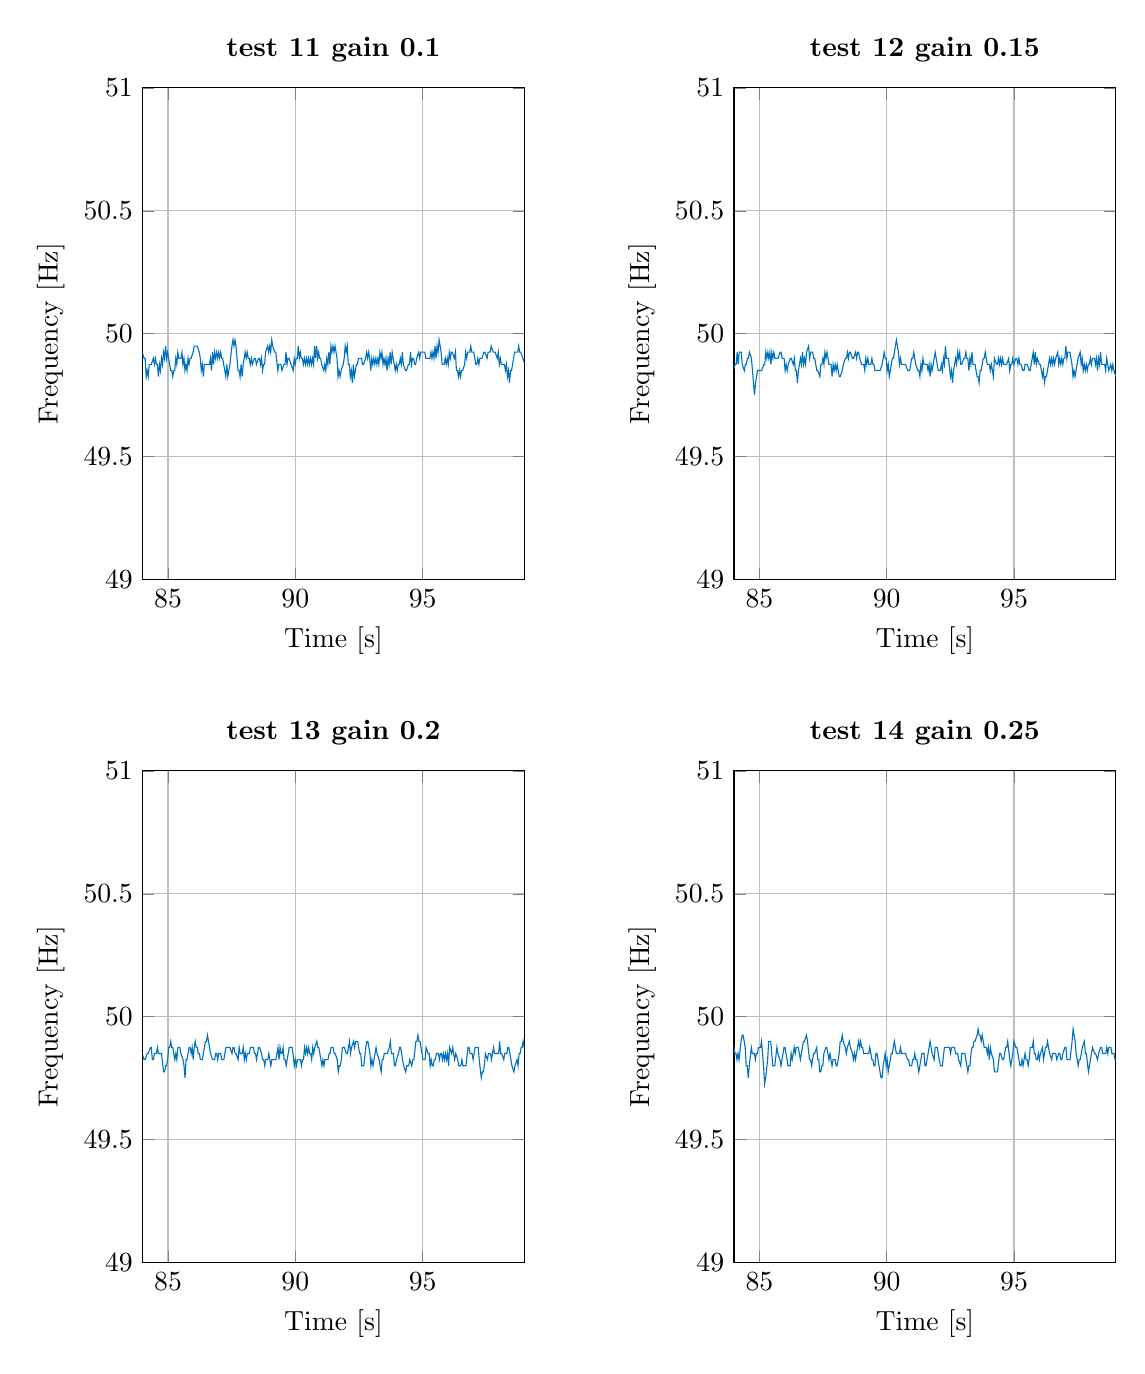
\begin{tikzpicture}

\begin{axis}[%
width=0.4\textwidth,
height=2.459in,
at={(1.043in,4.208in)},
scale only axis,
xmin=84,
xmax=99,
xlabel={Time [s]},
xmajorgrids,
ymin=49,
ymax=51,
ylabel={Frequency [Hz]},
ymajorgrids,
axis background/.style={fill=white},
title style={font=\bfseries},
title={test 11 gain 0.1}
]
\addplot [color=mycolor1,solid,forget plot]
  table[row sep=crcr]{%
83.9826	49.9251123315066\\
84.06272	49.9001996008121\\
84.1028	49.9001996007944\\
84.14288	49.825610363717\\
84.18302	49.8504486540534\\
84.22314	49.825610363717\\
84.26328	49.875311720704\\
84.30338	49.8753117206863\\
84.34348	49.875311720704\\
84.42368	49.9001996007944\\
84.46376	49.875311720704\\
84.50386	49.9001996007944\\
84.54394	49.875311720704\\
84.58404	49.8753117206863\\
84.62414	49.8256103637346\\
84.66428	49.875311720704\\
84.70438	49.8504486540358\\
84.7445	49.9001996007944\\
84.78458	49.875311720704\\
84.82468	49.9251123314889\\
84.86474	49.9001996008121\\
84.90482	49.950049950044\\
84.94486	49.9001996007944\\
84.98494	49.9251123315066\\
85.0651	49.8753117206863\\
85.1052	49.8504486540358\\
85.14532	49.8504486540534\\
85.18544	49.825610363717\\
85.22558	49.8504486540358\\
85.2657	49.8504486540358\\
85.30582	49.9001996008121\\
85.3459	49.8753117206863\\
85.386	49.9251123315066\\
85.42606	49.9001996007944\\
85.46614	49.9001996007944\\
85.50622	49.9001996008121\\
85.5463	49.9251123314889\\
85.58636	49.875311720704\\
85.62646	49.9001996007944\\
85.66654	49.8504486540358\\
85.70666	49.875311720704\\
85.74676	49.8504486540358\\
85.78688	49.9001996008121\\
85.82696	49.8753117206863\\
85.86706	49.9001996007944\\
85.90714	49.9001996008121\\
85.98728	49.9251123315066\\
86.02734	49.9500499500618\\
86.06738	49.950049950044\\
86.10742	49.950049950044\\
86.14746	49.9500499500618\\
86.22754	49.9251123315066\\
86.2676	49.9001996007944\\
86.30768	49.8504486540358\\
86.3478	49.875311720704\\
86.3879	49.825610363717\\
86.42804	49.875311720704\\
86.46814	49.875311720704\\
86.50824	49.8753117206863\\
86.54834	49.875311720704\\
86.62854	49.8753117206863\\
86.66864	49.9001996008121\\
86.70872	49.8504486540358\\
86.74884	49.9251123314889\\
86.7889	49.875311720704\\
86.829	49.9251123315066\\
86.86906	49.9001996007944\\
86.90914	49.9251123315066\\
86.9492	49.9001996007944\\
86.98928	49.9251123315066\\
87.02934	49.9001996007944\\
87.06942	49.9251123315066\\
87.10948	49.9001996007944\\
87.14956	49.9001996007944\\
87.18964	49.875311720704\\
87.26984	49.825610363717\\
87.30998	49.875311720704\\
87.35008	49.825610363717\\
87.39022	49.8504486540534\\
87.43034	49.8753117206863\\
87.5105	49.950049950044\\
87.55054	49.9750124937551\\
87.59056	49.9500499500618\\
87.6306	49.9750124937551\\
87.67062	49.950049950044\\
87.75072	49.8504486540358\\
87.79084	49.8504486540358\\
87.83096	49.825610363717\\
87.8711	49.875311720704\\
87.9112	49.8256103637346\\
87.95134	49.8753117206863\\
88.03152	49.9251123314889\\
88.07158	49.9001996008121\\
88.11166	49.9251123314889\\
88.15172	49.9001996008121\\
88.1918	49.9001996007944\\
88.23188	49.8753117206863\\
88.27198	49.9001996008121\\
88.31206	49.8753117206863\\
88.39226	49.9001996007944\\
88.43234	49.9001996008121\\
88.47242	49.8753117206863\\
88.5526	49.9001996008121\\
88.59268	49.9001996007944\\
88.63276	49.875311720704\\
88.67286	49.9001996007944\\
88.71294	49.8504486540358\\
88.75306	49.875311720704\\
88.79316	49.8753117206863\\
88.83326	49.9251123315066\\
88.91336	49.9500499500618\\
88.9534	49.9251123314889\\
88.99346	49.9500499500618\\
89.0335	49.9251123315066\\
89.07356	49.9750124937374\\
89.11358	49.9500499500618\\
89.19366	49.9251123315066\\
89.23372	49.9251123315066\\
89.31388	49.8504486540358\\
89.354	49.875311720704\\
89.4342	49.875311720704\\
89.4743	49.8504486540358\\
89.55454	49.8753117206863\\
89.59464	49.875311720704\\
89.63474	49.9251123315066\\
89.6748	49.875311720704\\
89.7149	49.9001996007944\\
89.75498	49.9001996007944\\
89.83514	49.875311720704\\
89.91534	49.8504486540358\\
89.95546	49.9001996007944\\
89.99554	49.875311720704\\
90.03564	49.9001996007944\\
90.07572	49.9001996007944\\
90.1158	49.950049950044\\
90.15584	49.9001996008121\\
90.19592	49.9251123314889\\
90.23598	49.9001996008121\\
90.27606	49.9001996007944\\
90.31614	49.875311720704\\
90.35624	49.9001996007944\\
90.39632	49.8753117206863\\
90.43642	49.9001996008121\\
90.4765	49.8753117206863\\
90.5166	49.9001996008121\\
90.55668	49.8753117206863\\
90.59678	49.9001996007944\\
90.63686	49.875311720704\\
90.67696	49.9001996007944\\
90.71704	49.875311720704\\
90.75714	49.950049950044\\
90.79718	49.9001996008121\\
90.83726	49.950049950044\\
90.8773	49.9001996007944\\
90.91738	49.9251123315066\\
90.95744	49.9001996007944\\
90.99752	49.9001996007944\\
91.0376	49.875311720704\\
91.1178	49.8504486540358\\
91.15792	49.875311720704\\
91.19802	49.8504486540358\\
91.23814	49.9001996007944\\
91.27822	49.875311720704\\
91.31832	49.9251123314889\\
91.35838	49.875311720704\\
91.39848	49.950049950044\\
91.43852	49.9251123315066\\
91.47858	49.950049950044\\
91.51862	49.9251123315066\\
91.55868	49.9500499500618\\
91.63878	49.9001996008121\\
91.67886	49.825610363717\\
91.719	49.8504486540358\\
91.75912	49.8256103637346\\
91.79926	49.8504486540358\\
91.8795	49.875311720704\\
91.9196	49.9001996007944\\
91.95968	49.950049950044\\
91.99972	49.9251123315066\\
92.03978	49.950049950044\\
92.07982	49.875311720704\\
92.11992	49.875311720704\\
92.16002	49.825610363717\\
92.20016	49.8504486540358\\
92.24028	49.8007968127488\\
92.28044	49.875311720704\\
92.32054	49.8256103637346\\
92.40078	49.875311720704\\
92.44088	49.875311720704\\
92.48098	49.9001996007944\\
92.52106	49.9001996007944\\
92.60122	49.9001996008121\\
92.6413	49.8753117206863\\
92.6814	49.875311720704\\
92.7616	49.9001996007944\\
92.80168	49.9251123315066\\
92.84174	49.9001996007944\\
92.88182	49.9251123315066\\
92.92188	49.9001996007944\\
92.96196	49.8504486540358\\
93.00208	49.9001996007944\\
93.04216	49.875311720704\\
93.08226	49.9001996007944\\
93.12234	49.875311720704\\
93.16244	49.9001996007944\\
93.20252	49.875311720704\\
93.24262	49.9001996007944\\
93.2827	49.875311720704\\
93.3228	49.9251123314889\\
93.36286	49.9001996008121\\
93.40294	49.9251123314889\\
93.443	49.875311720704\\
93.4831	49.9001996007944\\
93.52318	49.875311720704\\
93.56328	49.9001996007944\\
93.60336	49.8504486540358\\
93.64348	49.9001996008121\\
93.68356	49.8753117206863\\
93.72366	49.9251123315066\\
93.76372	49.875311720704\\
93.80382	49.9251123314889\\
93.84388	49.9001996008121\\
93.92406	49.8504486540534\\
93.96418	49.8753117206863\\
94.00428	49.8504486540358\\
94.0444	49.875311720704\\
94.0845	49.875311720704\\
94.1246	49.9001996007944\\
94.16468	49.875311720704\\
94.20478	49.9251123314889\\
94.24484	49.875311720704\\
94.32504	49.8504486540358\\
94.36516	49.8504486540358\\
94.4454	49.875311720704\\
94.4855	49.8753117206863\\
94.5256	49.9251123315066\\
94.56566	49.875311720704\\
94.60576	49.9001996007944\\
94.64584	49.9001996007944\\
94.68592	49.875311720704\\
94.72602	49.875311720704\\
94.76612	49.9001996007944\\
94.84628	49.9251123315066\\
94.88634	49.9001996007944\\
94.92642	49.9251123315066\\
94.96648	49.9251123315066\\
95.00654	49.9251123314889\\
95.0466	49.9251123315066\\
95.08666	49.9251123315066\\
95.12672	49.9001996007944\\
95.20688	49.9001996008121\\
95.24696	49.9001996007944\\
95.28704	49.9001996007944\\
95.32712	49.9251123315066\\
95.36718	49.9001996007944\\
95.40726	49.9251123315066\\
95.44732	49.9001996007944\\
95.4874	49.950049950044\\
95.52744	49.9001996008121\\
95.56752	49.950049950044\\
95.60756	49.9251123315066\\
95.64762	49.9750124937551\\
95.72768	49.9251123315066\\
95.76774	49.875311720704\\
95.80784	49.8753117206863\\
95.84794	49.875311720704\\
95.88804	49.9001996007944\\
95.92812	49.875311720704\\
95.96822	49.9001996007944\\
96.0083	49.875311720704\\
96.0484	49.9251123314889\\
96.08846	49.9001996008121\\
96.12854	49.9251123314889\\
96.1686	49.9251123315066\\
96.24872	49.9001996007944\\
96.2888	49.9251123315066\\
96.32886	49.8504486540358\\
96.36898	49.8504486540358\\
96.4091	49.8256103637346\\
96.44924	49.8504486540358\\
96.48936	49.8256103637346\\
96.5295	49.8504486540358\\
96.56962	49.8504486540358\\
96.64984	49.875311720704\\
96.68994	49.9251123315066\\
96.73	49.9001996007944\\
96.77008	49.9251123315066\\
96.8502	49.9251123314889\\
96.89026	49.9500499500618\\
96.9303	49.9251123315066\\
96.97036	49.9251123314889\\
97.01042	49.9251123315066\\
97.05048	49.9001996007944\\
97.09056	49.875311720704\\
97.13066	49.875311720704\\
97.17076	49.9001996007944\\
97.21084	49.875311720704\\
97.25094	49.9001996007944\\
97.29102	49.9001996007944\\
97.3311	49.9001996007944\\
97.41126	49.9251123314889\\
97.45132	49.9251123315066\\
97.53144	49.9001996007944\\
97.57152	49.9251123315066\\
97.65164	49.9251123314889\\
97.6917	49.9500499500618\\
97.7718	49.9251123314889\\
97.81186	49.9251123315066\\
97.85192	49.9251123315066\\
97.93204	49.9001996007944\\
97.97212	49.9251123315066\\
98.01218	49.8753117206863\\
98.05228	49.9001996008121\\
98.09236	49.8753117206863\\
98.13246	49.875311720704\\
98.17256	49.875311720704\\
98.21266	49.8753117206863\\
98.25276	49.8504486540358\\
98.29288	49.875311720704\\
98.33298	49.8256103637346\\
98.37312	49.8504486540358\\
98.41324	49.8007968127488\\
98.4534	49.8504486540358\\
98.49352	49.8504486540358\\
98.57374	49.9001996007944\\
98.61382	49.9251123315066\\
98.65388	49.9251123314889\\
98.69394	49.9251123315066\\
98.734	49.9251123315066\\
98.77406	49.950049950044\\
98.8141	49.9251123315066\\
98.85416	49.9251123315066\\
98.93428	49.9001996007944\\
99.01444	49.875311720704\\
};
\end{axis}

\begin{axis}[%
width=0.4\textwidth,
height=2.459in,
at={(4in,4.208in)},
scale only axis,
xmin=84,
xmax=99,
xlabel={Time [s]},
xmajorgrids,
ymin=49,
ymax=51,
ylabel={Frequency [Hz]},
ymajorgrids,
axis background/.style={fill=white},
title style={font=\bfseries},
title={test 12  gain 0.15}
]
\addplot [color=mycolor1,solid,forget plot]
  table[row sep=crcr]{%
83.96602	49.8504486540358\\
84.04624	49.875311720704\\
84.08634	49.875311720704\\
84.12644	49.9251123314889\\
84.1665	49.875311720704\\
84.2066	49.9251123315066\\
84.28672	49.9251123314889\\
84.32678	49.875311720704\\
84.40698	49.8504486540358\\
84.4471	49.875311720704\\
84.4872	49.8753117206863\\
84.5273	49.9001996008121\\
84.56738	49.9001996007944\\
84.60746	49.9251123315066\\
84.68758	49.9001996008121\\
84.72766	49.8504486540358\\
84.80792	49.7512437810962\\
84.84812	49.8007968127488\\
84.92844	49.8504486540358\\
84.96856	49.8504486540358\\
85.00868	49.8504486540534\\
85.0488	49.8504486540358\\
85.08892	49.8504486540358\\
85.16916	49.875311720704\\
85.20926	49.8753117206863\\
85.24936	49.9251123315066\\
85.28942	49.9001996007944\\
85.3295	49.9251123315066\\
85.36956	49.9001996007944\\
85.40964	49.9251123315066\\
85.4497	49.875311720704\\
85.4898	49.9251123314889\\
85.52986	49.9001996008121\\
85.56994	49.9251123314889\\
85.61	49.9001996008121\\
85.65008	49.9001996007944\\
85.69016	49.9001996007944\\
85.73024	49.9001996007944\\
85.8104	49.9251123314889\\
85.85046	49.9251123315066\\
85.89052	49.9001996007944\\
85.9306	49.9001996008121\\
85.97068	49.9001996007944\\
86.01076	49.8504486540358\\
86.05088	49.875311720704\\
86.09098	49.8504486540358\\
86.1311	49.8753117206863\\
86.2113	49.9001996007944\\
86.25138	49.9001996008121\\
86.33154	49.8753117206863\\
86.37164	49.9001996008121\\
86.41172	49.8504486540358\\
86.45184	49.8504486540358\\
86.49196	49.8007968127488\\
86.53212	49.8504486540358\\
86.61236	49.9001996007944\\
86.65244	49.875311720704\\
86.69254	49.9251123315066\\
86.7326	49.875311720704\\
86.7727	49.9001996007944\\
86.81278	49.8753117206863\\
86.85288	49.9251123315066\\
86.933	49.950049950044\\
86.97304	49.9001996008121\\
87.01312	49.9251123314889\\
87.05318	49.9251123315066\\
87.09324	49.9251123315066\\
87.1333	49.9001996007944\\
87.17338	49.9001996007944\\
87.25356	49.8504486540358\\
87.29368	49.8504486540358\\
87.37392	49.8256103637346\\
87.41406	49.875311720704\\
87.45416	49.8753117206863\\
87.49426	49.9001996008121\\
87.53434	49.8753117206863\\
87.57444	49.9251123315066\\
87.6145	49.9001996007944\\
87.65458	49.9251123315066\\
87.73472	49.875311720704\\
87.77482	49.875311720704\\
87.81492	49.8753117206863\\
87.85502	49.8256103637346\\
87.89516	49.875311720704\\
87.93526	49.8504486540358\\
87.97538	49.8753117206863\\
88.01548	49.8504486540358\\
88.0556	49.875311720704\\
88.13582	49.8256103637346\\
88.17596	49.825610363717\\
88.25622	49.8504486540534\\
88.29634	49.8753117206863\\
88.37652	49.9001996008121\\
88.4166	49.9001996007944\\
88.45668	49.9251123315066\\
88.49674	49.9001996007944\\
88.53682	49.9251123315066\\
88.57688	49.9251123315066\\
88.657	49.9001996008121\\
88.69708	49.9001996007944\\
88.77724	49.9251123315066\\
88.8173	49.9001996007944\\
88.85738	49.9251123315066\\
88.89744	49.9251123315066\\
88.9375	49.9001996007944\\
89.01766	49.875311720704\\
89.05776	49.8753117206863\\
89.09786	49.875311720704\\
89.13796	49.8504486540358\\
89.17808	49.9001996007944\\
89.21816	49.875311720704\\
89.25826	49.9001996007944\\
89.29834	49.875311720704\\
89.37854	49.8753117206863\\
89.41864	49.9001996008121\\
89.45872	49.8753117206863\\
89.49882	49.875311720704\\
89.53892	49.8504486540358\\
89.57904	49.8504486540358\\
89.61916	49.8504486540358\\
89.6994	49.8504486540358\\
89.73952	49.8504486540534\\
89.81974	49.875311720704\\
89.85984	49.9001996007944\\
89.89992	49.9251123315066\\
89.93998	49.9001996007944\\
89.98006	49.9001996007944\\
90.02014	49.8504486540534\\
90.06026	49.8753117206863\\
90.10036	49.8256103637346\\
90.18062	49.875311720704\\
90.22072	49.9001996007944\\
90.2608	49.9001996007944\\
90.34092	49.9500499500618\\
90.38096	49.9750124937551\\
90.46102	49.9251123315066\\
90.50108	49.8753117206863\\
90.54118	49.9001996008121\\
90.58126	49.8753117206863\\
90.62136	49.875311720704\\
90.70156	49.8753117206863\\
90.74166	49.875311720704\\
90.82186	49.8504486540358\\
90.86198	49.8504486540358\\
90.9021	49.8504486540358\\
90.98232	49.9001996007944\\
91.0224	49.9001996007944\\
91.06248	49.9251123315066\\
91.10254	49.9001996007944\\
91.14262	49.875311720704\\
91.22282	49.8504486540534\\
91.26294	49.8504486540358\\
91.30306	49.825610363717\\
91.3432	49.875311720704\\
91.3833	49.8504486540358\\
91.42342	49.9001996007944\\
91.4635	49.875311720704\\
91.5036	49.875311720704\\
91.5437	49.8753117206863\\
91.5838	49.875311720704\\
91.6239	49.8504486540358\\
91.66402	49.875311720704\\
91.70412	49.825610363717\\
91.74426	49.875311720704\\
91.78436	49.8504486540358\\
91.86458	49.9001996007944\\
91.90466	49.9251123315066\\
91.98482	49.8753117206863\\
92.02492	49.8504486540358\\
92.10516	49.8504486540534\\
92.14528	49.8753117206863\\
92.18538	49.8504486540358\\
92.2255	49.9001996008121\\
92.26558	49.8753117206863\\
92.30568	49.9500499500618\\
92.34572	49.9001996007944\\
92.3858	49.9001996007944\\
92.42588	49.9001996007944\\
92.50606	49.825610363717\\
92.5462	49.8504486540534\\
92.58632	49.8007968127488\\
92.62648	49.8504486540358\\
92.6666	49.8753117206863\\
92.7067	49.9001996008121\\
92.74678	49.8753117206863\\
92.78688	49.9251123315066\\
92.82694	49.9001996007944\\
92.86702	49.9251123315066\\
92.90708	49.875311720704\\
92.94718	49.8753117206863\\
93.02738	49.9001996007944\\
93.06746	49.9001996008121\\
93.10754	49.9251123314889\\
93.1476	49.9001996008121\\
93.18768	49.9001996007944\\
93.22776	49.8504486540358\\
93.26788	49.9001996007944\\
93.30796	49.875311720704\\
93.34806	49.9251123315066\\
93.38812	49.8753117206863\\
93.42822	49.875311720704\\
93.46832	49.875311720704\\
93.54854	49.825610363717\\
93.58868	49.8256103637346\\
93.62882	49.8007968127488\\
93.66898	49.8504486540358\\
93.7091	49.8504486540358\\
93.7893	49.9001996008121\\
93.82938	49.9001996007944\\
93.86946	49.9251123315066\\
93.90952	49.9001996007944\\
93.9496	49.875311720704\\
93.9897	49.8753117206863\\
94.0298	49.875311720704\\
94.0699	49.8504486540358\\
94.11002	49.875311720704\\
94.19022	49.8256103637346\\
94.23036	49.9001996007944\\
94.31054	49.8753117206863\\
94.35064	49.875311720704\\
94.39074	49.9001996007944\\
94.43082	49.875311720704\\
94.47092	49.9001996007944\\
94.511	49.875311720704\\
94.5511	49.9001996007944\\
94.59118	49.875311720704\\
94.63128	49.875311720704\\
94.67138	49.8753117206863\\
94.71148	49.875311720704\\
94.79168	49.9001996007944\\
94.83176	49.8504486540358\\
94.87188	49.875311720704\\
94.91198	49.8753117206863\\
94.95208	49.9001996007944\\
94.99216	49.875311720704\\
95.07236	49.9001996007944\\
95.11244	49.9001996007944\\
95.15252	49.875311720704\\
95.19262	49.9001996007944\\
95.2327	49.875311720704\\
95.2728	49.875311720704\\
95.353	49.8504486540358\\
95.39312	49.8504486540358\\
95.43324	49.875311720704\\
95.47334	49.875311720704\\
95.51344	49.8753117206863\\
95.59366	49.8504486540358\\
95.63378	49.8504486540358\\
95.714	49.9001996008121\\
95.75408	49.9251123315066\\
95.79414	49.8753117206863\\
95.83424	49.9251123315066\\
95.8743	49.875311720704\\
95.9144	49.9001996007944\\
95.99456	49.875311720704\\
96.03466	49.8753117206863\\
96.11488	49.825610363717\\
96.15502	49.8504486540358\\
96.19514	49.8007968127488\\
96.2353	49.8256103637346\\
96.27544	49.825610363717\\
96.3557	49.8753117206863\\
96.3958	49.9001996007944\\
96.43588	49.875311720704\\
96.47598	49.9001996007944\\
96.51606	49.875311720704\\
96.55616	49.9001996007944\\
96.59624	49.875311720704\\
96.63634	49.9001996007944\\
96.7165	49.9251123315066\\
96.75656	49.875311720704\\
96.79666	49.9001996007944\\
96.83674	49.875311720704\\
96.87684	49.9001996007944\\
96.91692	49.875311720704\\
96.95702	49.9001996007944\\
96.9971	49.9001996007944\\
97.03718	49.950049950044\\
97.07722	49.9001996008121\\
97.1173	49.9251123314889\\
97.15736	49.9251123315066\\
97.19742	49.9251123315066\\
97.27756	49.875311720704\\
97.31766	49.825610363717\\
97.3578	49.8504486540534\\
97.39792	49.825610363717\\
97.43806	49.8504486540358\\
97.51828	49.9001996007944\\
97.59844	49.9251123315066\\
97.6385	49.875311720704\\
97.6786	49.9001996007944\\
97.71868	49.8504486540358\\
97.7588	49.875311720704\\
97.7989	49.8504486540358\\
97.83902	49.875311720704\\
97.87912	49.8504486540358\\
97.91924	49.8753117206863\\
97.95934	49.875311720704\\
97.99944	49.9001996007944\\
98.03952	49.875311720704\\
98.07962	49.9001996007944\\
98.15978	49.9001996008121\\
98.19986	49.8753117206863\\
98.23996	49.9001996008121\\
98.28004	49.8504486540358\\
98.32016	49.9001996007944\\
98.36024	49.875311720704\\
98.40034	49.9251123314889\\
98.4404	49.875311720704\\
98.4805	49.875311720704\\
98.5206	49.8753117206863\\
98.5607	49.875311720704\\
98.6008	49.8504486540358\\
98.64092	49.9001996007944\\
98.681	49.875311720704\\
98.7211	49.8504486540358\\
98.80134	49.875311720704\\
98.84144	49.8504486540358\\
98.88156	49.875311720704\\
98.92166	49.8504486540358\\
99.0019	49.8256103637346\\
};
\end{axis}

\begin{axis}[%
width=0.4\textwidth,
height=2.459in,
at={(1.043in,0.793in)},
scale only axis,
xmin=84,
xmax=99,
xlabel={Time [s]},
xmajorgrids,
ymin=49,
ymax=51,
ylabel={Frequency [Hz]},
ymajorgrids,
axis background/.style={fill=white},
title style={font=\bfseries},
title={test 13  gain 0.2}
]
\addplot [color=mycolor1,solid,forget plot]
  table[row sep=crcr]{%
83.98314	49.8504486540358\\
84.06338	49.8256103637346\\
84.10352	49.825610363717\\
84.18378	49.8504486540534\\
84.2239	49.8504486540358\\
84.30412	49.875311720704\\
84.34422	49.875311720704\\
84.38432	49.825610363717\\
84.42446	49.8256103637346\\
84.4646	49.8504486540358\\
84.54484	49.8504486540358\\
84.58496	49.875311720704\\
84.62506	49.8504486540358\\
84.7053	49.8504486540358\\
84.74542	49.8504486540358\\
84.8257	49.7760079641708\\
84.86588	49.7760079641532\\
84.90606	49.8007968127488\\
84.94622	49.8007968127488\\
84.98638	49.8256103637346\\
85.02652	49.875311720704\\
85.06662	49.8753117206863\\
85.10672	49.9001996007944\\
85.1468	49.875311720704\\
85.1869	49.875311720704\\
85.227	49.8504486540358\\
85.26712	49.825610363717\\
85.30726	49.8504486540534\\
85.34738	49.825610363717\\
85.38752	49.875311720704\\
85.46772	49.8753117206863\\
85.50782	49.8504486540358\\
85.58806	49.8256103637346\\
85.6282	49.8007968127488\\
85.66836	49.7512437810962\\
85.70856	49.825610363717\\
85.7487	49.8256103637346\\
85.82896	49.875311720704\\
85.86906	49.875311720704\\
85.90916	49.8504486540358\\
85.94928	49.8753117206863\\
85.98938	49.8256103637346\\
86.02952	49.875311720704\\
86.06962	49.9001996007944\\
86.1097	49.8753117206863\\
86.1498	49.875311720704\\
86.1899	49.8504486540358\\
86.23002	49.8504486540358\\
86.27014	49.8256103637346\\
86.35042	49.825610363717\\
86.39056	49.8504486540358\\
86.47078	49.9001996007944\\
86.51086	49.9001996007944\\
86.55094	49.9251123315066\\
86.63108	49.875311720704\\
86.67118	49.8504486540358\\
86.75144	49.825610363717\\
86.79158	49.8256103637346\\
86.83172	49.825610363717\\
86.87186	49.8504486540534\\
86.91198	49.8504486540358\\
86.9521	49.825610363717\\
86.99224	49.8504486540358\\
87.07248	49.8504486540534\\
87.1126	49.825610363717\\
87.15274	49.8256103637346\\
87.19288	49.825610363717\\
87.27314	49.875311720704\\
87.31324	49.875311720704\\
87.35334	49.8753117206863\\
87.39344	49.875311720704\\
87.43354	49.875311720704\\
87.51374	49.8504486540534\\
87.55386	49.8753117206863\\
87.59396	49.875311720704\\
87.63406	49.8504486540358\\
87.67418	49.8504486540358\\
87.75442	49.8256103637346\\
87.79456	49.875311720704\\
87.83466	49.8504486540358\\
87.9149	49.8504486540358\\
87.95502	49.875311720704\\
87.99512	49.825610363717\\
88.03526	49.8504486540358\\
88.07538	49.8256103637346\\
88.11552	49.8504486540358\\
88.15564	49.8504486540358\\
88.19576	49.8504486540358\\
88.23588	49.875311720704\\
88.27598	49.875311720704\\
88.31608	49.8753117206863\\
88.35618	49.875311720704\\
88.39628	49.8504486540358\\
88.4364	49.8504486540358\\
88.47652	49.8256103637346\\
88.55678	49.8753117206863\\
88.59688	49.875311720704\\
88.67708	49.8504486540358\\
88.7172	49.825610363717\\
88.75734	49.8256103637346\\
88.79748	49.8007968127488\\
88.83764	49.8256103637346\\
88.87778	49.825610363717\\
88.91792	49.8256103637346\\
88.95806	49.8504486540358\\
89.03832	49.8007968127488\\
89.07848	49.8256103637346\\
89.11862	49.8256103637346\\
89.15876	49.825610363717\\
89.1989	49.8256103637346\\
89.23904	49.825610363717\\
89.3193	49.875311720704\\
89.3594	49.8256103637346\\
89.39954	49.8753117206863\\
89.43964	49.8504486540358\\
89.47976	49.8504486540534\\
89.51988	49.8753117206863\\
89.55998	49.8256103637346\\
89.60012	49.825610363717\\
89.64026	49.8007968127488\\
89.68042	49.8256103637346\\
89.72056	49.8504486540358\\
89.76068	49.875311720704\\
89.80078	49.8753117206863\\
89.84088	49.875311720704\\
89.88098	49.875311720704\\
89.96122	49.8007968127488\\
90.00138	49.8256103637346\\
90.04152	49.8007968127488\\
90.08168	49.8256103637346\\
90.12182	49.825610363717\\
90.16196	49.8256103637346\\
90.2021	49.825610363717\\
90.24224	49.8007968127488\\
90.2824	49.8256103637346\\
90.32254	49.825610363717\\
90.36268	49.875311720704\\
90.40278	49.8504486540358\\
90.4429	49.875311720704\\
90.483	49.8504486540358\\
90.52312	49.875311720704\\
90.56322	49.8504486540358\\
90.60334	49.8504486540358\\
90.64346	49.825610363717\\
90.6836	49.875311720704\\
90.7237	49.8504486540358\\
90.76382	49.875311720704\\
90.84402	49.9001996007944\\
90.8841	49.8753117206863\\
90.9242	49.875311720704\\
91.00442	49.8256103637346\\
91.04456	49.8007968127488\\
91.08472	49.825610363717\\
91.12486	49.8007968127488\\
91.16502	49.8256103637346\\
91.2453	49.825610363717\\
91.28544	49.8256103637346\\
91.32558	49.8504486540358\\
91.3657	49.8504486540358\\
91.40582	49.875311720704\\
91.44592	49.8753117206863\\
91.48602	49.875311720704\\
91.52612	49.8504486540358\\
91.56624	49.8504486540358\\
91.6465	49.825610363717\\
91.68664	49.7760079641708\\
91.72682	49.8007968127488\\
91.76698	49.8007968127488\\
91.80714	49.825610363717\\
91.84728	49.875311720704\\
91.88738	49.875311720704\\
91.92748	49.8753117206863\\
92.0077	49.8504486540358\\
92.04782	49.8504486540358\\
92.12806	49.9001996007944\\
92.16814	49.8504486540358\\
92.20826	49.875311720704\\
92.28846	49.9001996007944\\
92.32854	49.875311720704\\
92.36864	49.9001996007944\\
92.40872	49.9001996007944\\
92.4488	49.9001996007944\\
92.52898	49.8504486540358\\
92.5691	49.8504486540358\\
92.60922	49.8007968127488\\
92.64938	49.8007968127488\\
92.68954	49.8007968127488\\
92.76982	49.875311720704\\
92.80992	49.9001996007944\\
92.85	49.9001996007944\\
92.9302	49.8504486540358\\
92.97032	49.8007968127488\\
93.01048	49.825610363717\\
93.05062	49.8007968127488\\
93.09078	49.8256103637346\\
93.17104	49.875311720704\\
93.21114	49.8504486540358\\
93.29138	49.825610363717\\
93.33152	49.8007968127488\\
93.37168	49.7760079641708\\
93.41186	49.825610363717\\
93.452	49.8256103637346\\
93.49214	49.8504486540358\\
93.57238	49.8504486540358\\
93.6125	49.8504486540358\\
93.69274	49.8753117206863\\
93.73284	49.9001996008121\\
93.77292	49.8504486540358\\
93.81304	49.8504486540358\\
93.85316	49.8504486540358\\
93.89328	49.8007968127488\\
93.93344	49.8007968127488\\
93.9736	49.825610363717\\
94.05388	49.8504486540358\\
94.094	49.875311720704\\
94.1341	49.875311720704\\
94.21432	49.825610363717\\
94.25446	49.8007968127488\\
94.3348	49.7760079641532\\
94.37498	49.8007968127488\\
94.4553	49.8007968127488\\
94.49546	49.8256103637346\\
94.57574	49.8007968127488\\
94.6159	49.8256103637346\\
94.65604	49.825610363717\\
94.7363	49.9001996007944\\
94.77638	49.9001996007944\\
94.81646	49.9251123315066\\
94.85652	49.9001996007944\\
94.8966	49.9001996007944\\
94.97678	49.8504486540358\\
95.0169	49.8256103637346\\
95.05704	49.825610363717\\
95.09718	49.8256103637346\\
95.13732	49.8753117206863\\
95.21754	49.8504486540358\\
95.25766	49.8504486540358\\
95.29778	49.8007968127488\\
95.33794	49.825610363717\\
95.37808	49.8007968127488\\
95.41824	49.8007968127488\\
95.4584	49.8256103637346\\
95.49854	49.8256103637346\\
95.53868	49.8504486540358\\
95.61892	49.8504486540358\\
95.65904	49.825610363717\\
95.69918	49.8504486540534\\
95.7393	49.8504486540358\\
95.77942	49.825610363717\\
95.81956	49.8504486540358\\
95.85968	49.8256103637346\\
95.89982	49.8504486540358\\
95.93994	49.8256103637346\\
95.98008	49.8504486540358\\
96.0202	49.8007968127488\\
96.06036	49.8753117206863\\
96.14058	49.8504486540358\\
96.1807	49.8753117206863\\
96.26092	49.825610363717\\
96.30106	49.8504486540358\\
96.38132	49.825610363717\\
96.42146	49.8007968127488\\
96.50178	49.8007968127488\\
96.54194	49.8256103637346\\
96.58208	49.8007968127488\\
96.6624	49.8007968127488\\
96.70256	49.8007968127488\\
96.78286	49.8753117206863\\
96.82296	49.875311720704\\
96.86306	49.8504486540358\\
96.90318	49.8504486540358\\
96.9433	49.8504486540358\\
96.98342	49.8256103637346\\
97.02356	49.8504486540358\\
97.06368	49.875311720704\\
97.10378	49.8753117206863\\
97.14388	49.875311720704\\
97.18398	49.875311720704\\
97.22408	49.825610363717\\
97.30438	49.7512437810962\\
97.34458	49.7760079641708\\
97.38476	49.7760079641532\\
97.42494	49.8007968127488\\
97.4651	49.8504486540358\\
97.54534	49.8256103637346\\
97.58548	49.8504486540358\\
97.66572	49.8504486540358\\
97.70584	49.8256103637346\\
97.7861	49.875311720704\\
97.8262	49.8504486540358\\
97.86632	49.8504486540358\\
97.94656	49.8504486540358\\
97.98668	49.8504486540358\\
98.0268	49.9001996007944\\
98.06688	49.8504486540534\\
98.107	49.8504486540358\\
98.18724	49.825610363717\\
98.22738	49.8504486540358\\
98.2675	49.8504486540534\\
98.30762	49.8504486540358\\
98.34774	49.8753117206863\\
98.38784	49.875311720704\\
98.42794	49.8504486540358\\
98.46806	49.8256103637346\\
98.5082	49.8007968127488\\
98.58852	49.7760079641532\\
98.6287	49.8007968127488\\
98.70902	49.8256103637346\\
98.74916	49.8007968127488\\
98.78932	49.8504486540358\\
98.82944	49.8504486540358\\
98.86956	49.875311720704\\
98.90966	49.8753117206863\\
98.94976	49.9001996008121\\
98.98984	49.8753117206863\\
99.02994	49.875311720704\\
};
\end{axis}

\begin{axis}[%
width=0.4\textwidth,
height=2.459in,
at={(4in,0.793in)},
scale only axis,
xmin=84,
xmax=99,
xlabel={Time [s]},
xmajorgrids,
ymin=49,
ymax=51,
ylabel={Frequency [Hz]},
ymajorgrids,
axis background/.style={fill=white},
title style={font=\bfseries},
title={test 14  gain 0.25}
]
\addplot [color=mycolor1,solid,forget plot]
  table[row sep=crcr]{%
83.96004	49.8504486540358\\
84.00016	49.875311720704\\
84.04026	49.8504486540358\\
84.08038	49.8504486540358\\
84.1205	49.8256103637346\\
84.16064	49.8504486540358\\
84.20076	49.825610363717\\
84.28102	49.9001996008121\\
84.3211	49.9251123314889\\
84.36116	49.9251123315066\\
84.40122	49.9001996007944\\
84.4413	49.875311720704\\
84.4814	49.8007968127488\\
84.52156	49.8007968127488\\
84.56172	49.7512437810962\\
84.60192	49.8007968127488\\
84.68222	49.8753117206863\\
84.72232	49.8504486540358\\
84.76244	49.8504486540534\\
84.80256	49.8504486540358\\
84.84268	49.825610363717\\
84.88282	49.8504486540358\\
84.92294	49.8504486540358\\
84.96306	49.875311720704\\
85.04326	49.8753117206863\\
85.08336	49.9001996008121\\
85.16358	49.8007968127488\\
85.20374	49.7265042267642\\
85.24396	49.7512437810962\\
85.32434	49.8256103637346\\
85.36448	49.9001996007944\\
85.44464	49.9001996007944\\
85.48472	49.8504486540358\\
85.52484	49.8007968127488\\
85.565	49.8007968127488\\
85.60516	49.8007968127488\\
85.68544	49.8753117206863\\
85.72554	49.8504486540358\\
85.80578	49.8256103637346\\
85.84592	49.8007968127488\\
85.88608	49.8256103637346\\
85.96634	49.8753117206863\\
86.00644	49.875311720704\\
86.08668	49.825610363717\\
86.12682	49.8007968127488\\
86.20714	49.8007968127488\\
86.2473	49.8504486540358\\
86.28742	49.8256103637346\\
86.32756	49.8504486540358\\
86.36768	49.875311720704\\
86.40778	49.8504486540358\\
86.4479	49.875311720704\\
86.488	49.8753117206863\\
86.5281	49.875311720704\\
86.60832	49.8256103637346\\
86.64846	49.8504486540358\\
86.7287	49.9001996007944\\
86.76878	49.9001996007944\\
86.84894	49.9251123315066\\
86.889	49.9001996007944\\
86.96918	49.8256103637346\\
87.00932	49.825610363717\\
87.04946	49.8007968127488\\
87.08962	49.8256103637346\\
87.12976	49.8504486540358\\
87.16988	49.8504486540358\\
87.25012	49.875311720704\\
87.29022	49.825610363717\\
87.33036	49.8256103637346\\
87.3705	49.7760079641532\\
87.41068	49.7760079641708\\
87.45086	49.8007968127488\\
87.49102	49.8007968127488\\
87.53118	49.8504486540358\\
87.61142	49.875311720704\\
87.65152	49.875311720704\\
87.73174	49.825610363717\\
87.77188	49.8504486540358\\
87.812	49.8256103637346\\
87.85214	49.8007968127488\\
87.8923	49.8256103637346\\
87.93244	49.825610363717\\
87.97258	49.8256103637346\\
88.01272	49.8007968127488\\
88.05288	49.8007968127488\\
88.13318	49.8504486540358\\
88.1733	49.9001996008121\\
88.21338	49.9001996007944\\
88.25346	49.9251123315066\\
88.29352	49.9001996007944\\
88.3737	49.8753117206863\\
88.4138	49.8504486540358\\
88.45392	49.875311720704\\
88.53412	49.9001996007944\\
88.5742	49.875311720704\\
88.6544	49.8504486540358\\
88.69452	49.8256103637346\\
88.73466	49.8504486540358\\
88.77478	49.8256103637346\\
88.81492	49.8504486540358\\
88.89516	49.9001996007944\\
88.93524	49.875311720704\\
88.97534	49.9001996007944\\
89.01542	49.875311720704\\
89.05552	49.8753117206863\\
89.09562	49.8504486540358\\
89.13574	49.8504486540534\\
89.17586	49.8504486540358\\
89.21598	49.8504486540358\\
89.29622	49.8504486540358\\
89.33634	49.875311720704\\
89.41654	49.8256103637346\\
89.45668	49.8256103637346\\
89.49682	49.8007968127488\\
89.53698	49.8007968127488\\
89.57714	49.8504486540358\\
89.61726	49.8504486540358\\
89.69752	49.8007968127488\\
89.73768	49.7760079641708\\
89.77786	49.7512437810962\\
89.81806	49.7512437810962\\
89.85826	49.8007968127488\\
89.93856	49.8504486540358\\
89.97868	49.8007968127488\\
90.01884	49.8256103637346\\
90.05898	49.7760079641532\\
90.09916	49.8007968127488\\
90.17948	49.8504486540534\\
90.2196	49.8504486540358\\
90.25972	49.8753117206863\\
90.29982	49.9001996008121\\
90.3399	49.8753117206863\\
90.38	49.8504486540358\\
90.46024	49.8504486540534\\
90.50036	49.8504486540358\\
90.54048	49.8753117206863\\
90.58058	49.8504486540534\\
90.6207	49.8504486540358\\
90.70094	49.8504486540358\\
90.74106	49.8504486540358\\
90.8213	49.8256103637346\\
90.86144	49.825610363717\\
90.90158	49.8007968127488\\
90.9819	49.8007968127488\\
91.02206	49.8256103637346\\
91.0622	49.825610363717\\
91.10234	49.8504486540534\\
91.14246	49.825610363717\\
91.1826	49.8256103637346\\
91.22274	49.8007968127488\\
91.2629	49.7760079641532\\
91.34324	49.8256103637346\\
91.38338	49.8504486540358\\
91.46362	49.8504486540358\\
91.50374	49.8007968127488\\
91.5439	49.8007968127488\\
91.6242	49.8504486540358\\
91.66432	49.8753117206863\\
91.70442	49.9001996008121\\
91.7445	49.8753117206863\\
91.7846	49.8504486540534\\
91.86484	49.825610363717\\
91.90498	49.875311720704\\
91.98518	49.8753117206863\\
92.02528	49.8504486540358\\
92.10554	49.8007968127488\\
92.1457	49.8007968127488\\
92.18586	49.8007968127488\\
92.26614	49.875311720704\\
92.30624	49.8753117206863\\
92.34634	49.875311720704\\
92.38644	49.875311720704\\
92.42654	49.8753117206863\\
92.46664	49.875311720704\\
92.50674	49.8504486540358\\
92.54686	49.875311720704\\
92.62706	49.8753117206863\\
92.66716	49.875311720704\\
92.70726	49.8504486540358\\
92.74738	49.8504486540358\\
92.7875	49.8504486540358\\
92.82762	49.8256103637346\\
92.9079	49.8007968127488\\
92.94806	49.8504486540534\\
92.98818	49.8504486540358\\
93.0283	49.8504486540358\\
93.06842	49.8504486540358\\
93.14868	49.8007968127664\\
93.18884	49.7760079641532\\
93.22902	49.8007968127488\\
93.26918	49.8007968127488\\
93.30934	49.8504486540358\\
93.34946	49.875311720704\\
93.38956	49.8753117206863\\
93.42966	49.9001996008121\\
93.46974	49.9001996007944\\
93.5499	49.9251123315066\\
93.58996	49.950049950044\\
93.63	49.9251123315066\\
93.67006	49.9251123315066\\
93.71012	49.9001996007944\\
93.7502	49.9251123315066\\
93.79026	49.9001996007944\\
93.83034	49.875311720704\\
93.87044	49.8753117206863\\
93.91054	49.875311720704\\
93.95064	49.8504486540358\\
93.99076	49.875311720704\\
94.03086	49.825610363717\\
94.071	49.875311720704\\
94.1111	49.8504486540358\\
94.19134	49.8256103637346\\
94.23148	49.7760079641532\\
94.27166	49.7760079641708\\
94.31184	49.7760079641532\\
94.35202	49.7760079641708\\
94.43236	49.8504486540358\\
94.47248	49.8504486540358\\
94.55272	49.8256103637346\\
94.59286	49.825610363717\\
94.633	49.8504486540358\\
94.67312	49.875311720704\\
94.71322	49.875311720704\\
94.75332	49.9001996007944\\
94.83352	49.8256103637346\\
94.87366	49.8007968127488\\
94.95396	49.8504486540358\\
94.99408	49.9001996008121\\
95.07424	49.8753117206863\\
95.11434	49.875311720704\\
95.19456	49.8256103637346\\
95.2347	49.8007968127488\\
95.27486	49.8007968127488\\
95.31502	49.825610363717\\
95.35516	49.8007968127488\\
95.39532	49.8256103637346\\
95.43546	49.8504486540358\\
95.47558	49.8256103637346\\
95.51572	49.825610363717\\
95.55586	49.8007968127488\\
95.59602	49.8256103637346\\
95.63616	49.875311720704\\
95.67626	49.8753117206863\\
95.71636	49.875311720704\\
95.75646	49.9001996007944\\
95.79654	49.8504486540358\\
95.83666	49.8504486540358\\
95.87678	49.8256103637346\\
95.91692	49.825610363717\\
95.95706	49.8504486540534\\
95.99718	49.825610363717\\
96.03732	49.8504486540358\\
96.11756	49.875311720704\\
96.15766	49.8256103637346\\
96.23792	49.8753117206863\\
96.27802	49.875311720704\\
96.31812	49.9001996007944\\
96.3582	49.875311720704\\
96.3983	49.8504486540358\\
96.47856	49.825610363717\\
96.5187	49.8504486540358\\
96.55882	49.8504486540534\\
96.59894	49.8504486540358\\
96.63906	49.8504486540358\\
96.67918	49.825610363717\\
96.75944	49.8504486540534\\
96.79956	49.8504486540358\\
96.83968	49.825610363717\\
96.87982	49.8256103637346\\
96.91996	49.8504486540358\\
97.0002	49.875311720704\\
97.0403	49.8753117206863\\
97.0804	49.8256103637346\\
97.12054	49.8256103637346\\
97.16068	49.825610363717\\
97.20082	49.8256103637346\\
97.28106	49.9001996008121\\
97.32114	49.950049950044\\
97.40124	49.9001996007944\\
97.44132	49.8504486540358\\
97.52156	49.8007968127488\\
97.56172	49.8256103637346\\
97.60186	49.825610363717\\
97.642	49.8504486540358\\
97.68212	49.875311720704\\
97.7623	49.9001996008121\\
97.80238	49.8504486540358\\
97.8425	49.8504486540358\\
97.92278	49.7760079641532\\
97.96296	49.8007968127488\\
98.04328	49.8504486540358\\
98.0834	49.875311720704\\
98.1636	49.8504486540358\\
98.20372	49.8504486540358\\
98.28396	49.8256103637346\\
98.3241	49.8504486540358\\
98.40432	49.875311720704\\
98.44442	49.875311720704\\
98.48452	49.8504486540358\\
98.56476	49.8504486540358\\
98.60488	49.8504486540358\\
98.645	49.875311720704\\
98.6851	49.8504486540358\\
98.72522	49.875311720704\\
98.76532	49.8753117206863\\
98.80542	49.875311720704\\
98.84552	49.8504486540358\\
98.92576	49.8504486540534\\
98.96588	49.825610363717\\
99.00602	49.8256103637346\\
};
\end{axis}
\end{tikzpicture}%
\caption{Steady state at 50 kW load, with various scaling factors.}
\label{fig:test11-14steadyfrequency50kw}
\end{figure}

\subsubsection{Power}
\begin{figure}[H]
\centering
% This file was created by matlab2tikz.
%
%The latest updates can be retrieved from
%  http://www.mathworks.com/matlabcentral/fileexchange/22022-matlab2tikz-matlab2tikz
%where you can also make suggestions and rate matlab2tikz.
%
\definecolor{mycolor1}{rgb}{0.00000,0.44700,0.74100}%
%
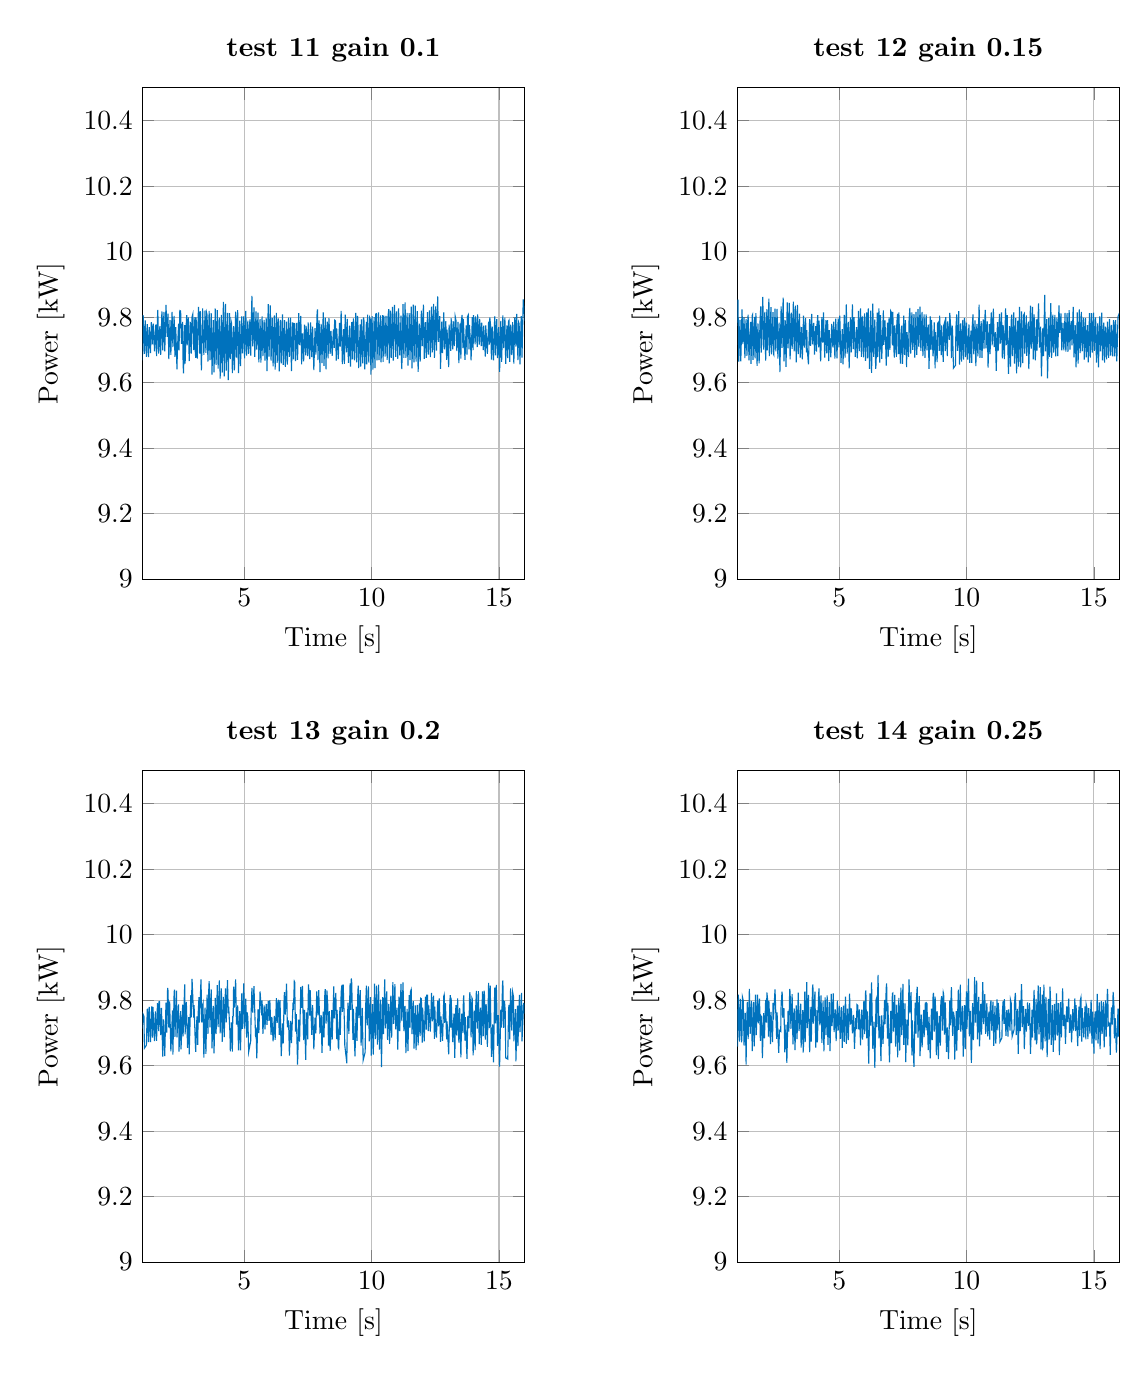
\begin{tikzpicture}

\begin{axis}[%
width=0.4\textwidth,
height=2.456in,
at={(1.026in,4.208in)},
scale only axis,
xmin=1,
xmax=16,
xlabel={Time [s]},
xmajorgrids,
ymin=9,
ymax=10.5,
ylabel={Power [kW]},
ymajorgrids,
axis background/.style={fill=white},
title style={font=\bfseries},
title={test 11 gain 0.1}
]
\addplot [color=mycolor1,solid,forget plot]
  table[row sep=crcr]{%
0.992	9.66807491828761\\
1.024	9.80578250722271\\
1.072	9.68805406147441\\
1.104	9.78996007093888\\
1.152	9.678747258028\\
1.184	9.77844187938428\\
1.232	9.6781006793502\\
1.264	9.76961154652533\\
1.312	9.68983721408203\\
1.344	9.78418806855951\\
1.36	9.77228655123696\\
1.392	9.71669722473514\\
1.424	9.77968902066963\\
1.472	9.69538374978654\\
1.52	9.77707421460958\\
1.552	9.68111079887103\\
1.584	9.79414711242576\\
1.6	9.82204953572795\\
1.632	9.68821777757661\\
1.68	9.77252843807131\\
1.712	9.68456523168112\\
1.76	9.81749731264033\\
1.776	9.79083948394269\\
1.792	9.69837457803596\\
1.84	9.81573626223996\\
1.872	9.6951080502519\\
1.888	9.73492220256255\\
1.92	9.8374131646726\\
1.968	9.73969548035118\\
2	9.81074047331049\\
2.032	9.67168024708054\\
2.08	9.79086741584716\\
2.112	9.68478717112037\\
2.128	9.73713540427954\\
2.16	9.8162404395391\\
2.192	9.70856771017066\\
2.24	9.80381430016023\\
2.272	9.67839933695742\\
2.304	9.76947869705412\\
2.352	9.64019904790587\\
2.368	9.69635927354901\\
2.416	9.77980176293947\\
2.432	9.69874764159959\\
2.464	9.81984955140141\\
2.496	9.81866873918375\\
2.528	9.71850560477925\\
2.576	9.7851599825776\\
2.592	9.66130370040842\\
2.608	9.62824494679215\\
2.656	9.7752738134272\\
2.672	9.65815688171727\\
2.72	9.78617623033648\\
2.736	9.8061871229451\\
2.752	9.71374561659831\\
2.8	9.79918779512\\
2.832	9.66543870216972\\
2.88	9.78535999123615\\
2.912	9.68840554885917\\
2.944	9.80018181252152\\
2.976	9.80983827166675\\
3.008	9.69884008713228\\
3.056	9.80005426214727\\
3.072	9.69311375653297\\
3.088	9.6754136687095\\
3.104	9.79886280176146\\
3.152	9.67333281036322\\
3.184	9.80212254819755\\
3.2	9.83129629346782\\
3.248	9.6886225533661\\
3.264	9.81830148708352\\
3.312	9.63752204550689\\
3.36	9.82643112754795\\
3.408	9.68465751899369\\
3.456	9.82083148490203\\
3.488	9.69101632233676\\
3.52	9.8115708665007\\
3.536	9.80612981047539\\
3.568	9.66382411635626\\
3.616	9.81925540783006\\
3.648	9.66830390066038\\
3.696	9.81212935050975\\
3.728	9.62472506564062\\
3.776	9.79079994115778\\
3.808	9.63098870750537\\
3.856	9.82622511096439\\
3.888	9.65393175288677\\
3.936	9.82112671288536\\
3.952	9.73645759983463\\
3.968	9.64305473967244\\
4.016	9.79859510511791\\
4.048	9.61203854601106\\
4.096	9.80688871894635\\
4.128	9.63050772653682\\
4.176	9.84638943047615\\
4.208	9.61879874571349\\
4.256	9.84053131611585\\
4.288	9.6365120122431\\
4.336	9.81254528175905\\
4.368	9.60766116470599\\
4.416	9.81188325888852\\
4.448	9.67162234552537\\
4.48	9.78690420880615\\
4.496	9.78142427535209\\
4.528	9.62866958328547\\
4.576	9.77244249625664\\
4.608	9.63710459654318\\
4.656	9.81646276740174\\
4.688	9.67609519478854\\
4.72	9.79303777866172\\
4.736	9.82104442908728\\
4.768	9.62882489017337\\
4.816	9.78883682082271\\
4.848	9.65030474192543\\
4.896	9.80192970252693\\
4.928	9.6891724397903\\
4.976	9.80239076075101\\
5.008	9.67407454665129\\
5.056	9.81914021331065\\
5.088	9.68253297083839\\
5.136	9.7890078748211\\
5.168	9.68789667395764\\
5.216	9.7933049133724\\
5.248	9.68251636731388\\
5.264	9.75777226080125\\
5.296	9.8650981041945\\
5.328	9.71071899851741\\
5.376	9.82981257467971\\
5.408	9.67858407649779\\
5.456	9.81764267898306\\
5.488	9.70046977245638\\
5.536	9.81350729366945\\
5.568	9.66153874355686\\
5.616	9.79353617765219\\
5.648	9.6613755722059\\
5.696	9.80240917066143\\
5.728	9.68073338555092\\
5.776	9.79178224711378\\
5.808	9.66680159898289\\
5.856	9.79658342372178\\
5.888	9.63529975670435\\
5.936	9.83921008375631\\
5.968	9.67907482057419\\
6.016	9.83540595721878\\
6.032	9.77090461507078\\
6.048	9.66684692763795\\
6.096	9.79766462758906\\
6.128	9.64956300230048\\
6.176	9.80545102384648\\
6.208	9.63991793091743\\
6.256	9.81266296286746\\
6.288	9.66000600469429\\
6.304	9.77094766629575\\
6.336	9.7963113759845\\
6.368	9.63453150265666\\
6.416	9.79166031764537\\
6.448	9.65874625767163\\
6.496	9.80823606239959\\
6.528	9.65406858223924\\
6.576	9.79076554441199\\
6.608	9.647985388507\\
6.64	9.72387348976243\\
6.656	9.78598022662435\\
6.688	9.65486668166624\\
6.736	9.79804970070713\\
6.768	9.67822134475062\\
6.816	9.79843735663189\\
6.848	9.63469413190914\\
6.896	9.7840170470172\\
6.928	9.67108323207966\\
6.944	9.78058229852132\\
6.976	9.78006725112338\\
7.008	9.66583540031059\\
7.056	9.78226635083368\\
7.088	9.66931612576336\\
7.136	9.81192241893913\\
7.168	9.71451937918574\\
7.216	9.80331756031752\\
7.248	9.65537129397429\\
7.28	9.75003472696907\\
7.328	9.66459683034395\\
7.36	9.77702793292656\\
7.408	9.68325758067465\\
7.424	9.77344226599558\\
7.488	9.6812112584763\\
7.504	9.78418544023736\\
7.568	9.67142487754972\\
7.6	9.78403826700439\\
7.648	9.67793070864908\\
7.68	9.77093859713965\\
7.728	9.63828100594682\\
7.776	9.7665897589137\\
7.808	9.68539390910054\\
7.856	9.81351271436875\\
7.872	9.82375366185007\\
7.888	9.66898825079454\\
7.936	9.79010084142839\\
7.968	9.63192571055096\\
7.984	9.71932292682433\\
8.016	9.77893630235422\\
8.048	9.65940878530751\\
8.096	9.81406285978542\\
8.128	9.6511816484286\\
8.176	9.7985175554744\\
8.208	9.6404696924428\\
8.224	9.74898479949512\\
8.256	9.78643185705628\\
8.288	9.67388420770426\\
8.32	9.79657011848653\\
8.336	9.76899110117059\\
8.368	9.6873967327966\\
8.4	9.75797372139604\\
8.448	9.68145028816503\\
8.496	9.76256603626151\\
8.528	9.70633285403859\\
8.544	9.79082678765671\\
8.576	9.78894587277734\\
8.608	9.6668587054772\\
8.624	9.76536162490897\\
8.688	9.67147359391963\\
8.736	9.78231352368705\\
8.768	9.71025100653491\\
8.8	9.81882568688327\\
8.848	9.65632614819931\\
8.896	9.76340791242335\\
8.928	9.65713642380071\\
8.96	9.80716584614058\\
9.008	9.69210445061006\\
9.04	9.79471986041107\\
9.088	9.66047048191917\\
9.136	9.77357323438136\\
9.168	9.64844457201364\\
9.216	9.78447081200709\\
9.248	9.67094697473589\\
9.28	9.79599329048386\\
9.328	9.66761294956789\\
9.344	9.74650041007152\\
9.376	9.81251782499848\\
9.408	9.66200818092358\\
9.44	9.8035152580934\\
9.456	9.79575395642999\\
9.488	9.64402547239994\\
9.552	9.77764919477466\\
9.568	9.64912801894788\\
9.584	9.70652173876579\\
9.6	9.79274235259868\\
9.648	9.65856873990652\\
9.68	9.79924175046931\\
9.696	9.78996199214031\\
9.728	9.64026441675768\\
9.792	9.78524188625075\\
9.808	9.65554603609201\\
9.84	9.80719934507074\\
9.888	9.66119928146418\\
9.92	9.79805935736669\\
9.952	9.79184564948569\\
9.968	9.62449398036362\\
10.016	9.80312258072681\\
10.048	9.63936781341954\\
10.096	9.79968011583623\\
10.128	9.64414611018636\\
10.16	9.80920687402261\\
10.192	9.81057476807194\\
10.208	9.66809943276699\\
10.272	9.81408232058174\\
10.288	9.66837393041089\\
10.352	9.80534596298293\\
10.368	9.66177302744249\\
10.432	9.80594248310699\\
10.448	9.66311450133886\\
10.48	9.80411465181989\\
10.528	9.67940034521072\\
10.56	9.8036496720453\\
10.608	9.66967896323023\\
10.64	9.8011532260213\\
10.672	9.82420328165452\\
10.688	9.65872948175304\\
10.704	9.69253867614646\\
10.736	9.8200609021984\\
10.768	9.6757301329142\\
10.816	9.83123433334715\\
10.848	9.6674393624089\\
10.896	9.83710664135793\\
10.944	9.67834409777932\\
10.976	9.81734602356787\\
11.024	9.67284336120245\\
11.056	9.82684397605816\\
11.104	9.68323132261819\\
11.152	9.80419654072855\\
11.168	9.66897449629245\\
11.184	9.64153279103188\\
11.232	9.83943870932398\\
11.264	9.67533950202536\\
11.312	9.84475078948958\\
11.344	9.67516071320763\\
11.392	9.81266877627825\\
11.424	9.65157133044229\\
11.472	9.81241508859288\\
11.504	9.66834214414275\\
11.552	9.83191986846623\\
11.584	9.64377717328257\\
11.632	9.83777664167821\\
11.664	9.66210657844986\\
11.712	9.83466906051323\\
11.744	9.66379523337059\\
11.792	9.81832479117196\\
11.824	9.63306015254874\\
11.872	9.78036352656237\\
11.904	9.66371021585058\\
11.936	9.76468663412133\\
11.952	9.81975414027303\\
11.984	9.71113240781376\\
12.032	9.83818476193497\\
12.064	9.67216184841652\\
12.112	9.78431255781177\\
12.144	9.67528513743576\\
12.176	9.76380715898833\\
12.192	9.81526059639624\\
12.224	9.68532984809038\\
12.272	9.82063901957372\\
12.304	9.67761236403928\\
12.352	9.83195977364821\\
12.384	9.69245485010134\\
12.432	9.84049506121001\\
12.464	9.67551647956832\\
12.48	9.73353488160445\\
12.512	9.83285966310167\\
12.544	9.69764576731343\\
12.592	9.8636170358386\\
12.624	9.72453919639269\\
12.672	9.80302091951136\\
12.704	9.6421157186625\\
12.752	9.78598107145373\\
12.784	9.68998490445913\\
12.832	9.81474006507249\\
12.864	9.70134094296754\\
12.912	9.78798030716377\\
12.944	9.66917586818838\\
12.96	9.76181132669667\\
13.024	9.64728333253928\\
13.04	9.77726813191121\\
13.104	9.69672456048927\\
13.12	9.79679309592338\\
13.184	9.70121798117563\\
13.2	9.78773623686989\\
13.248	9.71108541899297\\
13.28	9.80214325844344\\
13.312	9.78924239902231\\
13.344	9.6964949082845\\
13.392	9.78545222509658\\
13.424	9.65954836006227\\
13.472	9.78056312587153\\
13.504	9.67290465672358\\
13.52	9.78717860110889\\
13.552	9.80643621050003\\
13.584	9.7053538650768\\
13.6	9.79432169615683\\
13.664	9.66922825363447\\
13.712	9.77449338590688\\
13.744	9.68573190578887\\
13.76	9.80071796053332\\
13.792	9.80642713329464\\
13.824	9.70119121707189\\
13.84	9.77560230634734\\
13.888	9.7139759209312\\
13.904	9.66793073146443\\
13.952	9.79986755228104\\
13.984	9.69879779593957\\
14	9.80573191586204\\
14.064	9.71683142458575\\
14.08	9.80232612392281\\
14.128	9.74371054709547\\
14.144	9.7080272783338\\
14.16	9.80800464370282\\
14.224	9.71621000755681\\
14.24	9.79422895780022\\
14.272	9.75981082448397\\
14.304	9.71119663703168\\
14.32	9.7831143656735\\
14.384	9.69900689605181\\
14.4	9.77365613931535\\
14.464	9.67902654356733\\
14.48	9.7745067974479\\
14.544	9.68794232267948\\
14.592	9.78616791074934\\
14.624	9.71632100244602\\
14.64	9.79894563009823\\
14.672	9.7734037597322\\
14.704	9.66982779740172\\
14.736	9.77061005996931\\
14.784	9.6679253791212\\
14.832	9.80226420043863\\
14.864	9.68327975089579\\
14.896	9.7795266349557\\
14.912	9.79385382212886\\
14.944	9.67499716575899\\
14.992	9.7691849104796\\
15.024	9.63267975175901\\
15.072	9.78852636816364\\
15.104	9.66294645286532\\
15.152	9.80524311982818\\
15.184	9.70555399149469\\
15.2	9.73634940221313\\
15.232	9.79865823074573\\
15.264	9.65716770403156\\
15.312	9.77442604120738\\
15.344	9.6745625138212\\
15.376	9.78694746558369\\
15.392	9.78986568081661\\
15.424	9.66330461892713\\
15.456	9.77670982484096\\
15.488	9.73013450155636\\
15.504	9.68385353885138\\
15.536	9.78436506948828\\
15.584	9.65787260825075\\
15.616	9.79537910664646\\
15.632	9.79656269836046\\
15.664	9.70965498372932\\
15.696	9.80951117753686\\
15.744	9.66828356685326\\
15.776	9.7830260897324\\
15.792	9.77890465650089\\
15.824	9.65551298475637\\
15.872	9.80325941305973\\
15.904	9.67629929422191\\
15.952	9.85382424546227\\
16.016	9.78731613034146\\
};
\end{axis}

\begin{axis}[%
width=0.4\textwidth,
height=2.456in,
at={(4in,4.208in)},
scale only axis,
xmin=1,
xmax=16,
xlabel={Time [s]},
xmajorgrids,
ymin=9,
ymax=10.5,
ylabel={Power [kW]},
ymajorgrids,
axis background/.style={fill=white},
title style={font=\bfseries},
title={test 12  gain 0.15}
]
\addplot [color=mycolor1,solid,forget plot]
  table[row sep=crcr]{%
0.992	9.78288078951252\\
1.024	9.85351731561095\\
1.056	9.66377138896712\\
1.104	9.79160085238529\\
1.136	9.66454016006907\\
1.184	9.82317906210906\\
1.216	9.71728578413011\\
1.264	9.7987530324833\\
1.296	9.67451951081147\\
1.344	9.7940077211715\\
1.376	9.68185445920971\\
1.408	9.78772173398542\\
1.424	9.80765768372389\\
1.456	9.66771615533367\\
1.52	9.78519651901446\\
1.536	9.65682401675293\\
1.584	9.8048554888936\\
1.6	9.80782746431677\\
1.616	9.66957534036438\\
1.68	9.80041732015291\\
1.696	9.67391128929133\\
1.728	9.81192896237924\\
1.776	9.65087485673163\\
1.808	9.78101511638695\\
1.856	9.65853488796675\\
1.888	9.78366143245687\\
1.92	9.83290597983325\\
1.936	9.69126482192615\\
1.952	9.7197615479944\\
2	9.86170482582536\\
2.032	9.70078246607058\\
2.08	9.81583299749776\\
2.112	9.66683756912905\\
2.16	9.8241033273321\\
2.176	9.69846975522019\\
2.24	9.85650502148265\\
2.256	9.68099164134495\\
2.32	9.83006630275699\\
2.336	9.68610460158425\\
2.4	9.81505071539194\\
2.416	9.68740864226869\\
2.432	9.68459631020439\\
2.48	9.82588354977955\\
2.512	9.695246573914\\
2.56	9.82502165112067\\
2.592	9.67318467504549\\
2.64	9.78303936779566\\
2.672	9.6320807543104\\
2.72	9.83241769643397\\
2.752	9.70599011750963\\
2.8	9.85960341779882\\
2.832	9.66514289151664\\
2.88	9.79033100705101\\
2.912	9.64813263718743\\
2.944	9.78482267369639\\
2.96	9.8452867688434\\
2.992	9.70444744351098\\
3.04	9.84346334570791\\
3.072	9.67091105502141\\
3.12	9.81324419393523\\
3.152	9.70311747918266\\
3.184	9.79692704668781\\
3.2	9.84688325594389\\
3.232	9.69563428746573\\
3.28	9.83470955015086\\
3.312	9.6617942319067\\
3.36	9.83752687739123\\
3.392	9.6869160757378\\
3.44	9.81059984072579\\
3.472	9.67621616762968\\
3.52	9.769574359519\\
3.536	9.71642194100737\\
3.552	9.67119544597236\\
3.6	9.80459016288913\\
3.632	9.70721145844626\\
3.68	9.7968235119859\\
3.712	9.69264796754403\\
3.728	9.75998618598327\\
3.744	9.7023303199062\\
3.792	9.6560149279691\\
3.84	9.79402320396957\\
3.872	9.71184390642127\\
3.92	9.80945113884272\\
3.952	9.71650828182049\\
4	9.78237340110311\\
4.032	9.68564523128399\\
4.08	9.77256206356447\\
4.112	9.69458529204715\\
4.128	9.77608180975098\\
4.16	9.80596445559158\\
4.192	9.70777441464704\\
4.208	9.78910494279901\\
4.272	9.66479672723657\\
4.32	9.80006065711553\\
4.352	9.72185538959444\\
4.384	9.81462381625767\\
4.432	9.67596121520698\\
4.48	9.79044424824616\\
4.512	9.68905194547709\\
4.544	9.79074959468623\\
4.592	9.6659712903476\\
4.608	9.76034287541093\\
4.672	9.6768603901202\\
4.704	9.77940944412468\\
4.752	9.70724869167548\\
4.784	9.78595174568443\\
4.832	9.67315575770047\\
4.864	9.79494306188455\\
4.896	9.73487969038766\\
4.912	9.67403533631214\\
4.96	9.79608838091848\\
4.992	9.70758013640923\\
5.024	9.80463167602904\\
5.072	9.66061778542399\\
5.12	9.76321952435114\\
5.136	9.72089310323593\\
5.152	9.65592810748824\\
5.2	9.80699871532002\\
5.232	9.67598292746989\\
5.28	9.8386760945719\\
5.312	9.68856334235199\\
5.36	9.78520792104898\\
5.392	9.64374757029416\\
5.44	9.7987731934901\\
5.472	9.69228612751558\\
5.52	9.83865923802705\\
5.552	9.7021103945082\\
5.584	9.7997810142079\\
5.632	9.67827090139601\\
5.68	9.76964095061645\\
5.712	9.6739742789939\\
5.76	9.8188443728705\\
5.792	9.69647291846725\\
5.84	9.82688646911195\\
5.872	9.67834210836882\\
5.904	9.7978419828127\\
5.92	9.79964679699644\\
5.952	9.67710552336887\\
6	9.8109595581157\\
6.032	9.6660227575996\\
6.08	9.81475661271341\\
6.112	9.67410706896543\\
6.144	9.82647953918204\\
6.192	9.64216079097\\
6.24	9.81948016166378\\
6.272	9.62956230268871\\
6.32	9.841381744349\\
6.352	9.67872751370676\\
6.4	9.79262817066842\\
6.432	9.64220419309401\\
6.448	9.6557555783665\\
6.496	9.81352151311761\\
6.512	9.67752164898778\\
6.56	9.82661117089075\\
6.592	9.66108743204983\\
6.624	9.80568074376984\\
6.672	9.67233010329024\\
6.736	9.82072606853084\\
6.752	9.71504628784937\\
6.8	9.78990749876616\\
6.848	9.65223388381344\\
6.896	9.78339233222059\\
6.928	9.67909315139108\\
6.96	9.79893197213881\\
6.992	9.69970121378446\\
7.024	9.818351884318\\
7.056	9.81299670691401\\
7.088	9.71391240610453\\
7.104	9.81587517368589\\
7.152	9.69599905579451\\
7.168	9.6763429101096\\
7.184	9.7744044254293\\
7.248	9.6789257043667\\
7.264	9.7837523031067\\
7.296	9.81010677550014\\
7.328	9.68702103341431\\
7.344	9.81459057132029\\
7.392	9.68433061442536\\
7.408	9.65804918902077\\
7.44	9.76468700765158\\
7.456	9.77373345097501\\
7.488	9.65692216163625\\
7.536	9.80474467695185\\
7.568	9.6848946627431\\
7.6	9.79070923628748\\
7.648	9.6470749887551\\
7.664	9.75427685746819\\
7.728	9.67832740637716\\
7.744	9.78902039348664\\
7.776	9.82799036843103\\
7.808	9.68836278864314\\
7.856	9.81465773061595\\
7.888	9.69965345002826\\
7.936	9.80882261464626\\
7.968	9.67647448598339\\
8.016	9.81607928304089\\
8.032	9.73678374952848\\
8.048	9.68460601015256\\
8.096	9.82450116834594\\
8.128	9.70874508588658\\
8.176	9.83176380252889\\
8.208	9.69705018892969\\
8.256	9.81564906183316\\
8.272	9.74309658038672\\
8.288	9.68055886806072\\
8.336	9.80839791200378\\
8.368	9.67529716169738\\
8.416	9.80827954287976\\
8.448	9.6981145323954\\
8.496	9.7768878513683\\
8.528	9.64222899992495\\
8.576	9.8023148642929\\
8.608	9.7008539207004\\
8.624	9.791311738486\\
8.688	9.67976375694559\\
8.736	9.7841382164504\\
8.768	9.64314202430947\\
8.784	9.75391323906244\\
8.848	9.6627115397495\\
8.864	9.78083373006774\\
8.896	9.78406940982193\\
8.928	9.69697036159305\\
8.944	9.80448539267339\\
9.008	9.68390884569223\\
9.024	9.77470532365756\\
9.088	9.66350134709766\\
9.104	9.7739298935304\\
9.136	9.78273915366495\\
9.168	9.69597861820691\\
9.184	9.80020170745745\\
9.248	9.68079509552442\\
9.264	9.78691053813264\\
9.328	9.73043539401508\\
9.344	9.81292885311926\\
9.392	9.75273655511732\\
9.408	9.67450254384224\\
9.44	9.77423463550458\\
9.456	9.75151918162463\\
9.488	9.64418119548103\\
9.568	9.65278214254711\\
9.584	9.7658921209332\\
9.616	9.80787306667721\\
9.648	9.69661354350924\\
9.696	9.81785826970592\\
9.728	9.65457486300651\\
9.776	9.78088094140423\\
9.808	9.66397588775048\\
9.856	9.79142195773626\\
9.888	9.66994173036423\\
9.92	9.79733377531756\\
9.936	9.78312595166995\\
9.968	9.67798722213979\\
10	9.78336399557458\\
10.048	9.67005295863196\\
10.096	9.77759244955701\\
10.128	9.66012885867596\\
10.176	9.75879379985385\\
10.208	9.66017087154819\\
10.224	9.76809411955302\\
10.256	9.80820676998955\\
10.288	9.68637438316275\\
10.336	9.79026214879776\\
10.368	9.65001504610219\\
10.4	9.76627866909998\\
10.416	9.77933397521114\\
10.448	9.6798865162626\\
10.496	9.83839526566526\\
10.528	9.67571240265676\\
10.576	9.78741205778958\\
10.608	9.67535362916137\\
10.656	9.7931220075356\\
10.688	9.70352132558775\\
10.704	9.75986843129201\\
10.736	9.82170471127999\\
10.752	9.79098326605518\\
10.768	9.7044906510966\\
10.816	9.78657180942123\\
10.848	9.64607646524819\\
10.896	9.77826660045523\\
10.928	9.686693727238\\
10.944	9.76214978944022\\
10.976	9.81442760203471\\
11.008	9.71386938311308\\
11.056	9.82570029468411\\
11.088	9.70828370157212\\
11.136	9.75413938288228\\
11.168	9.63565648603875\\
11.216	9.7843328122511\\
11.248	9.69739087735009\\
11.296	9.80970364008317\\
11.328	9.71873475667623\\
11.376	9.81443589134251\\
11.408	9.67362009146163\\
11.44	9.77565614037045\\
11.488	9.67197636570604\\
11.536	9.82674824165498\\
11.568	9.71431691891501\\
11.6	9.80636020025703\\
11.648	9.62639796306747\\
11.696	9.77247777036126\\
11.728	9.64864735955525\\
11.76	9.79265172650405\\
11.776	9.80750258054777\\
11.808	9.68072669883942\\
11.856	9.8147342404571\\
11.888	9.65828573391955\\
11.936	9.7967043750803\\
11.968	9.62834329723827\\
12.016	9.78943784343421\\
12.048	9.64907924886917\\
12.08	9.83103630733357\\
12.128	9.64661189689054\\
12.16	9.81774314725174\\
12.208	9.65980113233047\\
12.24	9.80580581861229\\
12.272	9.81045561716726\\
12.288	9.68826876604963\\
12.304	9.71972666047393\\
12.352	9.80496276699315\\
12.368	9.68143475081804\\
12.432	9.78581425199623\\
12.448	9.64113046585101\\
12.512	9.83526505819768\\
12.528	9.71627073113479\\
12.544	9.70380548486781\\
12.592	9.83128440983954\\
12.624	9.67060182089653\\
12.656	9.80802832913732\\
12.704	9.66778036104395\\
12.752	9.79271654226247\\
12.768	9.69761274277428\\
12.832	9.84177349325005\\
12.864	9.70700619269714\\
12.912	9.77082882750623\\
12.944	9.61930331609054\\
12.992	9.76584263399084\\
13.024	9.68088856152467\\
13.072	9.86777945980773\\
13.104	9.69537776686303\\
13.152	9.79389723223836\\
13.184	9.61258973388937\\
13.232	9.7973015333369\\
13.264	9.67887927466684\\
13.296	9.78713672692269\\
13.312	9.84274622773319\\
13.344	9.67555010677562\\
13.392	9.80770509482509\\
13.424	9.69166952059468\\
13.472	9.80652041203442\\
13.488	9.73919451082839\\
13.504	9.67999735728122\\
13.552	9.79854116381188\\
13.584	9.68062654064403\\
13.632	9.83567177337177\\
13.664	9.75159310545804\\
13.712	9.81094493892823\\
13.744	9.69828995783937\\
13.792	9.78202678471741\\
13.824	9.69824344107534\\
13.872	9.8127053267297\\
13.888	9.72445508971235\\
13.904	9.69468551710569\\
13.952	9.81216420521571\\
13.984	9.69414735127183\\
14.032	9.82153411532142\\
14.064	9.70059248293221\\
14.08	9.74785640209663\\
14.112	9.78847612912492\\
14.144	9.71349531661187\\
14.192	9.83128037996836\\
14.224	9.67688774057837\\
14.272	9.77506298266933\\
14.304	9.64637176710688\\
14.352	9.81462512739094\\
14.384	9.65775840975235\\
14.432	9.82352034335454\\
14.464	9.6900888453721\\
14.512	9.81557722841405\\
14.544	9.69561384018223\\
14.592	9.79866879942712\\
14.608	9.76225231048959\\
14.624	9.67016802621639\\
14.672	9.7977748834018\\
14.704	9.67695043665805\\
14.752	9.77533245934219\\
14.784	9.66211726980426\\
14.832	9.81245002676688\\
14.864	9.67605034768442\\
14.896	9.78529279560662\\
14.912	9.81218280584864\\
14.944	9.69168584646496\\
14.992	9.81383276147577\\
15.024	9.69676217288301\\
15.072	9.7988835644488\\
15.104	9.66088885651548\\
15.152	9.78076109484963\\
15.184	9.6468432433479\\
15.2	9.70729339421895\\
15.232	9.80223656714904\\
15.264	9.69559638017025\\
15.312	9.81364099973229\\
15.344	9.66800346930099\\
15.392	9.78338621653364\\
15.424	9.66109104018488\\
15.456	9.77062601065851\\
15.488	9.72213513506972\\
15.504	9.67064008570529\\
15.536	9.78622524609176\\
15.584	9.67562456681216\\
15.616	9.79414324870933\\
15.664	9.68274333830629\\
15.696	9.77647167957807\\
15.744	9.679743320304\\
15.776	9.79031715170937\\
15.792	9.77670223038695\\
15.824	9.6799939058245\\
15.856	9.79048798011118\\
15.904	9.66508998624241\\
15.952	9.80097397920783\\
16.016	9.81445745303067\\
};
\end{axis}

\begin{axis}[%
width=0.4\textwidth,
height=2.456in,
at={(1.026in,0.793in)},
scale only axis,
xmin=1,
xmax=16,
xlabel={Time [s]},
xmajorgrids,
ymin=9,
ymax=10.5,
ylabel={Power [kW]},
ymajorgrids,
axis background/.style={fill=white},
title style={font=\bfseries},
title={test 13  gain 0.2}
]
\addplot [color=mycolor1,solid,forget plot]
  table[row sep=crcr]{%
0.992	9.71267060384848\\
1.008	9.75939443569367\\
1.056	9.7501278303599\\
1.072	9.65294537357213\\
1.152	9.66226496343235\\
1.184	9.77133575581142\\
1.2	9.77197354323261\\
1.232	9.67169593016801\\
1.264	9.77930516527897\\
1.312	9.6715291685789\\
1.36	9.78081723637441\\
1.392	9.68569470756371\\
1.408	9.77928120867633\\
1.472	9.67501737110775\\
1.504	9.76554374788247\\
1.552	9.67569448386774\\
1.584	9.79100540389731\\
1.632	9.70527405552828\\
1.648	9.79491180356934\\
1.664	9.79548893687195\\
1.712	9.6933988095938\\
1.744	9.77637348585665\\
1.792	9.62768574125493\\
1.824	9.74090763481377\\
1.872	9.62860520475777\\
1.92	9.79244676350439\\
1.952	9.70049301418588\\
1.984	9.83745527667416\\
2	9.82865106688906\\
2.032	9.71563288243121\\
2.064	9.79635995550612\\
2.112	9.64343575642712\\
2.128	9.67241155042978\\
2.176	9.76819958842661\\
2.192	9.63345249999931\\
2.24	9.8233295838245\\
2.256	9.83169020560965\\
2.272	9.68783629833272\\
2.336	9.82917438193362\\
2.352	9.68633540486225\\
2.368	9.70895715942724\\
2.416	9.78701486530211\\
2.432	9.64285471434789\\
2.496	9.7661071884847\\
2.512	9.64961667684065\\
2.576	9.78586134200866\\
2.592	9.68952188725462\\
2.656	9.84822097794788\\
2.672	9.69545170440157\\
2.72	9.79454566530871\\
2.768	9.65439064226715\\
2.816	9.74804519245337\\
2.832	9.63419229175144\\
2.896	9.81529612171744\\
2.912	9.74735371636626\\
2.944	9.8649208576115\\
3.008	9.74653203943721\\
3.024	9.78428764213416\\
3.072	9.66821795533002\\
3.088	9.6420936411409\\
3.136	9.75012190820779\\
3.168	9.66308998052759\\
3.184	9.75791508216948\\
3.216	9.80900030819647\\
3.232	9.73098171511101\\
3.248	9.76349737955887\\
3.296	9.86335238849097\\
3.328	9.73121841371671\\
3.36	9.78051638200509\\
3.376	9.78712361696892\\
3.408	9.62428638584032\\
3.456	9.77681521777498\\
3.488	9.63565649378099\\
3.536	9.81681387955472\\
3.568	9.69654115880263\\
3.6	9.83047145969348\\
3.616	9.85784160812688\\
3.648	9.71708608699175\\
3.696	9.83270547228972\\
3.728	9.65252882348572\\
3.776	9.78209247081025\\
3.808	9.63739913501481\\
3.856	9.80637498678562\\
3.888	9.69701886847178\\
3.936	9.84604364461271\\
3.952	9.75380156676864\\
3.968	9.71761164272661\\
4.016	9.85990518365394\\
4.048	9.69845409890073\\
4.096	9.83565959868212\\
4.128	9.67252028379451\\
4.176	9.80962310174672\\
4.208	9.68702680316123\\
4.256	9.83545771151525\\
4.288	9.73203213715745\\
4.336	9.86093498612331\\
4.368	9.75996295388058\\
4.384	9.78027108668492\\
4.432	9.70046822903569\\
4.448	9.64367775705888\\
4.496	9.73213219885578\\
4.528	9.64263555162533\\
4.544	9.74939259673422\\
4.56	9.74916800319601\\
4.576	9.84107419845539\\
4.608	9.77712503863925\\
4.656	9.86355328865005\\
4.672	9.79347589188626\\
4.688	9.72532346951468\\
4.736	9.78413113253282\\
4.768	9.64667368497701\\
4.816	9.76658119967465\\
4.848	9.64623286602565\\
4.896	9.82080934821273\\
4.928	9.71216234116092\\
4.976	9.85127008079719\\
5.008	9.71275011762676\\
5.056	9.80443950044369\\
5.088	9.68539168294582\\
5.104	9.76275961716442\\
5.136	9.7484938071588\\
5.168	9.64180118419229\\
5.248	9.67502805714741\\
5.264	9.75695722716148\\
5.296	9.83759426685145\\
5.328	9.76167623896322\\
5.376	9.84237668062166\\
5.44	9.68694722182677\\
5.456	9.71640109856284\\
5.488	9.62201846473504\\
5.536	9.77128546369798\\
5.568	9.69917890791432\\
5.616	9.82643077996478\\
5.68	9.75369179080931\\
5.696	9.79900487629761\\
5.728	9.6971177289863\\
5.776	9.78363790055197\\
5.808	9.71090781831827\\
5.856	9.78852720914936\\
5.888	9.72476711104789\\
5.936	9.79723240179455\\
5.968	9.73636088758847\\
6	9.80015560158243\\
6.048	9.69357846412702\\
6.08	9.74874810860766\\
6.128	9.67389825691098\\
6.176	9.75146069109025\\
6.208	9.67891716299036\\
6.256	9.8059061077378\\
6.288	9.73055356750357\\
6.32	9.79092207290024\\
6.336	9.80099119962786\\
6.368	9.69371609851626\\
6.4	9.79960738145946\\
6.448	9.62869114972746\\
6.496	9.72905033869297\\
6.528	9.66788543531596\\
6.56	9.80621989462483\\
6.576	9.82430626392079\\
6.608	9.75589552686036\\
6.656	9.8504761216219\\
6.672	9.79057201813789\\
6.688	9.71707532152878\\
6.736	9.7380789976812\\
6.768	9.63032182392899\\
6.816	9.73625059423322\\
6.848	9.66830652259468\\
6.912	9.79288371393383\\
6.928	9.76997274765513\\
6.96	9.85759672816412\\
6.976	9.85520825052507\\
7.008	9.70366640607033\\
7.04	9.75705879985724\\
7.088	9.60290332855729\\
7.136	9.74019949907864\\
7.168	9.67343203130162\\
7.216	9.84013824315054\\
7.248	9.7766206333362\\
7.28	9.8431942264803\\
7.328	9.67800906824742\\
7.36	9.76981281779676\\
7.408	9.61748108224591\\
7.44	9.76224839806816\\
7.488	9.68019181477927\\
7.504	9.80056040919516\\
7.52	9.84763398391401\\
7.568	9.75294575482492\\
7.584	9.83064445577947\\
7.648	9.6937469097429\\
7.68	9.78457785064905\\
7.728	9.64988108644817\\
7.776	9.74639980820017\\
7.808	9.6984966329281\\
7.84	9.82650468190943\\
7.888	9.75378045887694\\
7.92	9.83070774630204\\
7.968	9.70077152356953\\
7.984	9.70227584051423\\
8.016	9.75397253930785\\
8.048	9.63857712022099\\
8.096	9.76444610448186\\
8.128	9.68622865928679\\
8.16	9.8216155753517\\
8.176	9.83361186715299\\
8.208	9.72805633378934\\
8.224	9.75596917336362\\
8.24	9.82973585397666\\
8.272	9.78994825086444\\
8.304	9.6611349631049\\
8.336	9.76601081047117\\
8.368	9.64502044015697\\
8.432	9.7696988457292\\
8.448	9.67951151395654\\
8.512	9.84193083565282\\
8.528	9.74419527187349\\
8.592	9.8222425843948\\
8.624	9.681064575044\\
8.64	9.76984314798842\\
8.688	9.65532296388939\\
8.704	9.65225028524362\\
8.752	9.77881194203315\\
8.768	9.69355049513257\\
8.8	9.82410038969532\\
8.832	9.84634672109098\\
8.848	9.76443199453243\\
8.88	9.84791066418746\\
8.928	9.73351335870646\\
8.944	9.66165235096947\\
9.024	9.60680411463775\\
9.04	9.72877192481996\\
9.072	9.79220712444803\\
9.104	9.69697625732645\\
9.152	9.85069509915565\\
9.168	9.76994111991235\\
9.2	9.86622197435759\\
9.216	9.85304855836668\\
9.264	9.67873748680436\\
9.28	9.77324196553007\\
9.344	9.62807275960362\\
9.392	9.7799246024723\\
9.424	9.67558837238955\\
9.456	9.82404720221533\\
9.472	9.84436246221372\\
9.504	9.74469393703657\\
9.552	9.83041942003978\\
9.584	9.66113454188466\\
9.632	9.77599857646372\\
9.664	9.61600598517057\\
9.744	9.64102942665825\\
9.76	9.77213406182464\\
9.792	9.84444817255487\\
9.808	9.77182668458686\\
9.824	9.72259607826179\\
9.872	9.84162445364447\\
9.904	9.67367746498516\\
9.952	9.80896817509162\\
9.984	9.63046972437263\\
10.032	9.78786053460628\\
10.064	9.63337056698683\\
10.112	9.85025720633516\\
10.144	9.68078535311919\\
10.192	9.84385758850125\\
10.224	9.66442647953748\\
10.272	9.84727506118193\\
10.304	9.64854024993446\\
10.352	9.80119807662837\\
10.384	9.59547909710779\\
10.432	9.80918519359152\\
10.464	9.6960940218566\\
10.512	9.86300756378714\\
10.528	9.78420485409159\\
10.544	9.71402544810341\\
10.592	9.82645906331771\\
10.624	9.67840803683857\\
10.672	9.7882876096139\\
10.704	9.66633555722899\\
10.752	9.81326326130556\\
10.784	9.68516359260886\\
10.832	9.85516992343999\\
10.864	9.72771968599621\\
10.912	9.84886109890591\\
10.944	9.71082416886495\\
10.992	9.77677679453424\\
11.024	9.64859024169858\\
11.072	9.81023507812694\\
11.104	9.70548596924731\\
11.12	9.77466119288007\\
11.152	9.8493807108308\\
11.184	9.73603557138112\\
11.232	9.85440680285175\\
11.264	9.70553541967405\\
11.312	9.78260515562421\\
11.344	9.63833013850448\\
11.392	9.77335055453153\\
11.424	9.64410483447988\\
11.472	9.81529093233189\\
11.504	9.71631914434909\\
11.52	9.82495973044613\\
11.552	9.83240186236163\\
11.584	9.69615006165253\\
11.632	9.79648920867906\\
11.664	9.65216865648264\\
11.712	9.78381879616324\\
11.744	9.64730847198027\\
11.792	9.78505257332678\\
11.824	9.66177701225983\\
11.872	9.78960490950229\\
11.904	9.68988702076647\\
11.92	9.80584850753299\\
11.952	9.80408721391632\\
11.984	9.67036226171792\\
12	9.77688633744069\\
12.064	9.67431086510698\\
12.112	9.81077070290373\\
12.144	9.70987259499796\\
12.16	9.81512402571194\\
12.192	9.81497540854467\\
12.224	9.70514705085242\\
12.24	9.78370576560561\\
12.304	9.70371787774607\\
12.352	9.8223071565448\\
12.384	9.73507723234374\\
12.432	9.81345352530895\\
12.464	9.68138293342165\\
12.48	9.78011835441126\\
12.496	9.73884642379359\\
12.544	9.68566991790575\\
12.592	9.79853790771193\\
12.624	9.72018768529489\\
12.656	9.80491366461342\\
12.704	9.67236498244061\\
12.72	9.75030405008055\\
12.784	9.67564532546504\\
12.832	9.81167865381076\\
12.848	9.81616483049377\\
12.864	9.73082046823786\\
12.896	9.79065778135894\\
12.944	9.68029409008654\\
12.96	9.73463618405516\\
13.024	9.6340451893047\\
13.072	9.79978630296308\\
13.088	9.81495079853483\\
13.104	9.71610247980671\\
13.12	9.80736002027522\\
13.184	9.67163662731646\\
13.232	9.75841054739907\\
13.264	9.62337409597929\\
13.296	9.76724840046725\\
13.312	9.78432710685851\\
13.344	9.69125829061936\\
13.376	9.80536781643434\\
13.424	9.67026186884411\\
13.456	9.77596224373655\\
13.504	9.62484891463424\\
13.536	9.75880408311761\\
13.584	9.69894727048975\\
13.6	9.79785398444914\\
13.616	9.8143292923701\\
13.664	9.67655469495235\\
13.68	9.74774439915319\\
13.744	9.62071321965718\\
13.776	9.75192777806737\\
13.824	9.71411703054837\\
13.84	9.79962120741838\\
13.856	9.8240371367009\\
13.888	9.77241344022452\\
13.904	9.68632831930175\\
13.936	9.80672170381671\\
13.952	9.8036952857643\\
13.984	9.63088899697659\\
14.032	9.76795816214758\\
14.064	9.64745219015394\\
14.08	9.76602476365682\\
14.112	9.82813581390181\\
14.144	9.71257342790625\\
14.192	9.82731777101852\\
14.224	9.66528059586574\\
14.272	9.77684254327433\\
14.304	9.66328947633505\\
14.352	9.82674381224606\\
14.384	9.69016812448973\\
14.416	9.82912060299231\\
14.432	9.81341817308566\\
14.464	9.67968273375209\\
14.496	9.78757012184654\\
14.544	9.65747896744753\\
14.592	9.85243818490091\\
14.624	9.71422613686552\\
14.656	9.84432470505391\\
14.704	9.62650964019536\\
14.752	9.72596981543182\\
14.784	9.6097161411691\\
14.832	9.83834902717335\\
14.864	9.72872954873213\\
14.896	9.84678644813306\\
14.944	9.66056867156052\\
14.976	9.75432858827723\\
15.024	9.59687987025055\\
15.072	9.7706570642194\\
15.104	9.71619275895986\\
15.136	9.84231719267945\\
15.152	9.86047450620418\\
15.184	9.71495293639918\\
15.2	9.7563066443121\\
15.216	9.79786901056496\\
15.248	9.76204693650815\\
15.264	9.62343415859966\\
15.344	9.61986054366048\\
15.376	9.77016989262102\\
15.392	9.78558710055853\\
15.424	9.68019165636468\\
15.44	9.7732567436616\\
15.456	9.83571084318207\\
15.504	9.70695877785523\\
15.536	9.82431118944767\\
15.568	9.8112713774675\\
15.584	9.67396360791687\\
15.648	9.77217837643683\\
15.664	9.61262200972749\\
15.728	9.78302537836562\\
15.744	9.65977399576615\\
15.792	9.79344470393688\\
15.808	9.81617556519873\\
15.824	9.70255197341671\\
15.888	9.82212705705806\\
15.904	9.67411018047097\\
15.968	9.79117272407463\\
16.016	9.7582435627018\\
};
\end{axis}

\begin{axis}[%
width=0.4\textwidth,
height=2.456in,
at={(4in,0.793in)},
scale only axis,
xmin=1,
xmax=16,
xlabel={Time [s]},
xmajorgrids,
ymin=9,
ymax=10.5,
ylabel={Power [kW]},
ymajorgrids,
axis background/.style={fill=white},
title style={font=\bfseries},
title={test 14  gain 0.25}
]
\addplot [color=mycolor1,solid,forget plot]
  table[row sep=crcr]{%
0.992	9.7715850777201\\
1.008	9.65779212194046\\
1.04	9.81682651785084\\
1.088	9.67300545679486\\
1.12	9.8037020566523\\
1.168	9.6710375140013\\
1.184	9.6964063460481\\
1.2	9.80949929080405\\
1.232	9.79909479634238\\
1.264	9.66097016373217\\
1.312	9.76083708815186\\
1.344	9.60292475506301\\
1.36	9.70701057583706\\
1.392	9.79437251734956\\
1.424	9.68111240118369\\
1.472	9.83416442533841\\
1.504	9.6970659819618\\
1.552	9.79746725210669\\
1.584	9.64405423328824\\
1.632	9.7944274387926\\
1.664	9.65891314115374\\
1.712	9.81676712672004\\
1.744	9.69308506772373\\
1.792	9.81655754401143\\
1.824	9.7293305202236\\
1.872	9.80422792657241\\
1.904	9.67569466911351\\
1.92	9.75285349987551\\
1.952	9.74841121387067\\
1.984	9.62287630341425\\
2.032	9.76030225250847\\
2.064	9.6834792027208\\
2.112	9.80096484226077\\
2.144	9.73142552562893\\
2.16	9.82339025814082\\
2.192	9.79984540451482\\
2.224	9.68876538048367\\
2.24	9.79644814628396\\
2.304	9.66524187139354\\
2.32	9.76393962362986\\
2.384	9.67194946520944\\
2.4	9.79163943569494\\
2.416	9.74073241216338\\
2.48	9.83288212324703\\
2.544	9.6819666813072\\
2.56	9.76248846034544\\
2.624	9.63861798308167\\
2.656	9.70740576805274\\
2.704	9.70431214183527\\
2.72	9.79749564761399\\
2.736	9.79686553900667\\
2.752	9.82602748895548\\
2.768	9.8151495431026\\
2.784	9.74667882498569\\
2.832	9.77501619487841\\
2.864	9.64060167671257\\
2.912	9.72520164798067\\
2.944	9.60834066668097\\
2.992	9.7668154798436\\
3.024	9.70354422500588\\
3.056	9.83382405160993\\
3.072	9.82627452106417\\
3.104	9.71205278049865\\
3.152	9.81828313933567\\
3.184	9.66512690872551\\
3.232	9.77492901351354\\
3.264	9.64733963013402\\
3.312	9.78421048856252\\
3.344	9.68093052607742\\
3.392	9.82287244810537\\
3.424	9.70551354113953\\
3.488	9.78895493022494\\
3.504	9.65476723318952\\
3.568	9.76927068334308\\
3.584	9.63981135313415\\
3.6	9.6624041594641\\
3.648	9.82613780304739\\
3.664	9.6713799569275\\
3.728	9.85496248972184\\
3.744	9.71453291784906\\
3.792	9.81625107763355\\
3.84	9.6407841582782\\
3.888	9.7795727071765\\
3.904	9.67314681175749\\
3.952	9.83682408584981\\
3.968	9.84777045196761\\
3.984	9.72813486243981\\
4.048	9.82561320251373\\
4.08	9.65477609330967\\
4.128	9.76895505324737\\
4.144	9.67090448496121\\
4.192	9.8167260337371\\
4.208	9.83549959170151\\
4.24	9.72268151944126\\
4.288	9.81421122326702\\
4.32	9.66972968866651\\
4.368	9.79706418461956\\
4.4	9.64349668629224\\
4.448	9.80838333970825\\
4.48	9.69323337882937\\
4.528	9.81454699422109\\
4.544	9.71875072402588\\
4.56	9.66312451102742\\
4.608	9.79485474675855\\
4.64	9.64389243313511\\
4.688	9.81886899917187\\
4.72	9.72052472564148\\
4.768	9.82071305250601\\
4.8	9.70263411863162\\
4.848	9.77147643591069\\
4.88	9.67445392946922\\
4.928	9.79848796040259\\
4.96	9.70714129100636\\
5.008	9.78203859916087\\
5.04	9.68157011909169\\
5.088	9.7787186267698\\
5.12	9.65386431446176\\
5.168	9.78302752169083\\
5.2	9.67283136861806\\
5.248	9.81059191480683\\
5.264	9.76112282578494\\
5.28	9.66617415540394\\
5.328	9.77393895051723\\
5.36	9.67749926185889\\
5.408	9.81939407395097\\
5.44	9.72489518679652\\
5.472	9.7744278293036\\
5.488	9.76072452327003\\
5.52	9.69830879915444\\
5.568	9.75492576064643\\
5.6	9.65144152604459\\
5.648	9.7452441283286\\
5.68	9.71150321694988\\
5.696	9.78624594872435\\
5.728	9.7837599272042\\
5.76	9.71037124938747\\
5.792	9.77149083761869\\
5.84	9.66194268410144\\
5.856	9.72530809718179\\
5.888	9.77087162053491\\
5.92	9.67918291883136\\
5.968	9.79735236859124\\
6	9.69630543011552\\
6.032	9.82043235819775\\
6.048	9.82953275470803\\
6.08	9.68345270950584\\
6.112	9.76563845530835\\
6.16	9.60589625077925\\
6.208	9.82026250598052\\
6.24	9.72199650179826\\
6.272	9.85375273044659\\
6.32	9.65148433451833\\
6.368	9.73383576317299\\
6.4	9.59272333135603\\
6.448	9.80059292467297\\
6.464	9.80469349541245\\
6.48	9.71747434367678\\
6.528	9.87726593199798\\
6.56	9.68319880864738\\
6.592	9.75187344238546\\
6.64	9.6138671452437\\
6.672	9.75317494084019\\
6.72	9.66652417994442\\
6.736	9.69797869028075\\
6.784	9.80085911552069\\
6.8	9.72644871758357\\
6.848	9.83850055492164\\
6.864	9.85064800660982\\
6.896	9.68224647271781\\
6.912	9.79180118521863\\
6.976	9.60954205703621\\
7.024	9.76714676235373\\
7.056	9.66892227169036\\
7.088	9.81964433532588\\
7.104	9.82105861028358\\
7.136	9.70370320063342\\
7.184	9.81611115666933\\
7.216	9.65797938712625\\
7.264	9.78623753369205\\
7.296	9.62524849592981\\
7.344	9.80707286263327\\
7.376	9.64584186400199\\
7.424	9.83811601064368\\
7.44	9.75295578776304\\
7.456	9.69336256810607\\
7.504	9.84937075360533\\
7.536	9.66363551625113\\
7.584	9.79014076416177\\
7.616	9.61058148641946\\
7.632	9.68442767941503\\
7.664	9.74011947453029\\
7.696	9.66151918363325\\
7.744	9.86343696542507\\
7.776	9.75977842183\\
7.824	9.82394864852792\\
7.856	9.6315802491484\\
7.872	9.73778384288329\\
7.936	9.59583265573104\\
7.984	9.79222037896084\\
8.016	9.69740355138505\\
8.032	9.80028712117928\\
8.064	9.84067786705665\\
8.096	9.68578447432406\\
8.144	9.8117913970696\\
8.16	9.75936602850208\\
8.176	9.6287776080215\\
8.224	9.75530650695196\\
8.256	9.65586956917115\\
8.32	9.7701677685013\\
8.336	9.68699814310141\\
8.384	9.79270186446932\\
8.416	9.70722909295158\\
8.432	9.79090025770195\\
8.448	9.78934644333013\\
8.496	9.64734115693286\\
8.528	9.74888341184368\\
8.576	9.62204898637583\\
8.624	9.77399515977479\\
8.656	9.67767849195256\\
8.688	9.81514065767178\\
8.704	9.82217861205924\\
8.736	9.70363178481542\\
8.768	9.81076067381504\\
8.8	9.74318118875364\\
8.816	9.63177692735498\\
8.848	9.7666202877188\\
8.896	9.61970796840191\\
8.928	9.751880580848\\
8.976	9.66114065542369\\
8.992	9.79278570182063\\
9.024	9.81197154461865\\
9.04	9.78223337828609\\
9.056	9.70716755405403\\
9.088	9.82311335543949\\
9.104	9.8176737130127\\
9.136	9.69488045180773\\
9.168	9.79268357245524\\
9.216	9.64166554900846\\
9.248	9.71658478477878\\
9.296	9.620165441282\\
9.344	9.79816856528533\\
9.376	9.72285149510913\\
9.392	9.80276681854337\\
9.408	9.8396112412101\\
9.456	9.69088589466337\\
9.488	9.76481600747665\\
9.52	9.74718418137247\\
9.536	9.61825293407827\\
9.6	9.76615063983936\\
9.616	9.64566298173302\\
9.632	9.69827373421517\\
9.68	9.8317695618281\\
9.696	9.70901169350903\\
9.76	9.84752969470747\\
9.776	9.70365915851532\\
9.84	9.78251367971001\\
9.872	9.62751338083558\\
9.92	9.78497393172802\\
9.952	9.65053697226231\\
9.984	9.78644500169131\\
10	9.82625349736914\\
10.016	9.71240519320598\\
10.08	9.86531479540633\\
10.112	9.68950309573215\\
10.16	9.76668991892206\\
10.176	9.65724724808646\\
10.192	9.6082746997582\\
10.224	9.71151493337406\\
10.24	9.79070400680649\\
10.272	9.6775232280181\\
10.32	9.86980937311098\\
10.352	9.73157532212711\\
10.4	9.85917224938635\\
10.432	9.67992731224296\\
10.48	9.80990789523853\\
10.512	9.65860302651825\\
10.56	9.78838661809626\\
10.576	9.72453466436016\\
10.592	9.69450613728619\\
10.64	9.85489076635807\\
10.672	9.72676554878593\\
10.72	9.81840715996539\\
10.752	9.69667385669877\\
10.8	9.79080038102692\\
10.832	9.68900599363201\\
10.88	9.76507814403141\\
10.912	9.6796859905077\\
10.928	9.77487512907815\\
10.96	9.79924388383632\\
10.992	9.70680522061616\\
11.04	9.79555968617077\\
11.072	9.66049880693632\\
11.12	9.78209719417962\\
11.152	9.66689024085066\\
11.2	9.80225500162865\\
11.232	9.70793683475638\\
11.248	9.79156853978749\\
11.296	9.73415725348767\\
11.312	9.67247652560545\\
11.392	9.68518881617784\\
11.408	9.76192676707147\\
11.44	9.7977131030991\\
11.472	9.72756465232458\\
11.488	9.80318113859312\\
11.552	9.69060621638786\\
11.584	9.76966729437921\\
11.632	9.68833496241196\\
11.648	9.77155112075047\\
11.712	9.70658010987724\\
11.728	9.80069226901746\\
11.76	9.78980760985948\\
11.792	9.68842617502194\\
11.872	9.71046220336051\\
11.888	9.79241114900372\\
11.92	9.82175692632724\\
11.936	9.78471813646741\\
11.952	9.69336013529642\\
12	9.77299418591388\\
12.032	9.6358053656797\\
12.08	9.79920812119721\\
12.112	9.70501075428414\\
12.128	9.75865110079284\\
12.16	9.84845620061163\\
12.176	9.81628017761468\\
12.192	9.71773525096253\\
12.24	9.78166650510175\\
12.272	9.65001220340996\\
12.32	9.77291080954379\\
12.352	9.70410235545171\\
12.4	9.79335117318527\\
12.432	9.72160571341944\\
12.48	9.79032521551914\\
12.512	9.63574235488624\\
12.576	9.77074427348163\\
12.592	9.68582458628342\\
12.656	9.83139637717112\\
12.688	9.67673825797024\\
12.736	9.80335716468476\\
12.752	9.66457953513996\\
12.768	9.67817588125508\\
12.816	9.84514965216641\\
12.848	9.69506869987026\\
12.896	9.83951702212176\\
12.928	9.64951285549493\\
12.976	9.81690493163422\\
12.992	9.65259848138937\\
13.008	9.65548977357042\\
13.04	9.84734979965562\\
13.088	9.67412685070202\\
13.12	9.80973923062286\\
13.168	9.62578941026068\\
13.216	9.8038854599415\\
13.248	9.67906673634553\\
13.28	9.84094093343682\\
13.296	9.81366328523001\\
13.328	9.66332300909409\\
13.376	9.78455178526702\\
13.408	9.64194326825492\\
13.456	9.78835976935125\\
13.488	9.6767018436361\\
13.536	9.82034079945396\\
13.568	9.69172513622373\\
13.616	9.79094747978284\\
13.648	9.63197020636689\\
13.696	9.79344455396146\\
13.712	9.73075240807482\\
13.728	9.68595908846784\\
13.776	9.83602546748609\\
13.808	9.72047285409072\\
13.856	9.75532245852409\\
13.888	9.66640828141997\\
13.936	9.78048128201331\\
13.968	9.73253311648961\\
14.016	9.80469935852215\\
14.048	9.70008943525055\\
14.096	9.75600428449968\\
14.128	9.67108785522665\\
14.176	9.77270030361053\\
14.208	9.70713621677401\\
14.256	9.80524661015487\\
14.288	9.70555612844053\\
14.304	9.78463888532118\\
14.368	9.65966562271184\\
14.416	9.78002443286542\\
14.448	9.68998332772927\\
14.464	9.79754749972729\\
14.496	9.80812971959723\\
14.528	9.67294860708042\\
14.544	9.77554492288612\\
14.608	9.68632663168668\\
14.656	9.78054319293665\\
14.688	9.68010901975502\\
14.704	9.78634610621473\\
14.736	9.77445215856939\\
14.768	9.68054448099977\\
14.8	9.77542621658524\\
14.848	9.69793558881044\\
14.896	9.80088834357692\\
14.928	9.66711343481799\\
14.96	9.76501193091389\\
15.008	9.63657793935906\\
15.024	9.72699877818077\\
15.056	9.76577071716671\\
15.088	9.67698471863765\\
15.136	9.81894647189696\\
15.168	9.66695591172582\\
15.216	9.79265826741672\\
15.248	9.65053043820026\\
15.296	9.79695939399436\\
15.328	9.69666620102287\\
15.376	9.79480926776789\\
15.408	9.65553324079765\\
15.456	9.79892411652694\\
15.488	9.68880119744409\\
15.536	9.83408839332066\\
15.552	9.80967386196057\\
15.568	9.72293778574758\\
15.616	9.72812408013142\\
15.648	9.632696534266\\
15.664	9.71929133944831\\
15.696	9.77803799062175\\
15.728	9.72513479227548\\
15.76	9.82487774790767\\
15.792	9.7827645768597\\
15.808	9.68311493721902\\
15.84	9.74501867251978\\
15.888	9.63978723678914\\
15.952	9.77415089192634\\
15.968	9.68851932525071\\
16.016	9.78157984221207\\
};
\end{axis}
\end{tikzpicture}%
\caption{Steady state at 10 kW load, with various scaling factors.}
\label{fig:test11-14steadypower10kw}
\end{figure}

\begin{figure}[H]
\centering
% This file was created by matlab2tikz.
%
%The latest updates can be retrieved from
%  http://www.mathworks.com/matlabcentral/fileexchange/22022-matlab2tikz-matlab2tikz
%where you can also make suggestions and rate matlab2tikz.
%
\definecolor{mycolor1}{rgb}{0.00000,0.44700,0.74100}%
%
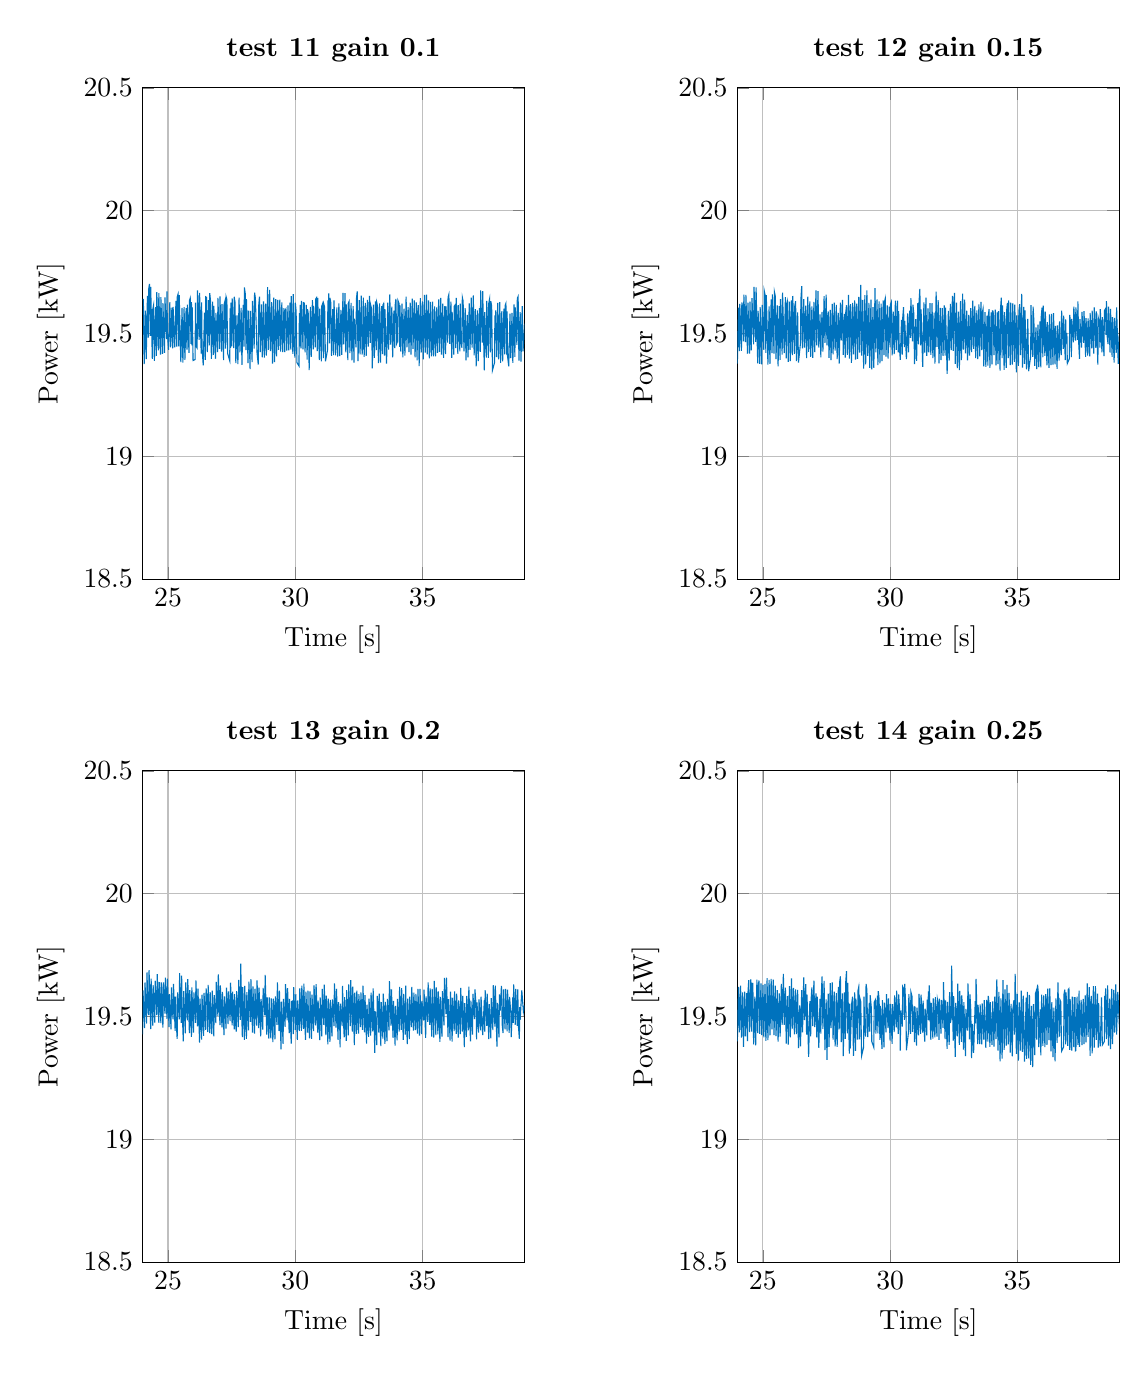
\begin{tikzpicture}

\begin{axis}[%
width=0.4\textwidth,
height=2.456in,
at={(1.026in,4.208in)},
scale only axis,
xmin=24,
xmax=39,
xlabel={Time [s]},
xmajorgrids,
ymin=18.5,
ymax=20.5,
ylabel={Power [kW]},
ymajorgrids,
axis background/.style={fill=white},
title style={font=\bfseries},
title={test 11 gain 0.1}
]
\addplot [color=mycolor1,solid,forget plot]
  table[row sep=crcr]{%
24	19.6381373554797\\
24.032	19.6384254161173\\
24.064	19.3751748531885\\
24.112	19.5925296921381\\
24.144	19.3955399074198\\
24.192	19.6525897177572\\
24.224	19.4832579161225\\
24.24	19.6797865028412\\
24.272	19.7020122563309\\
24.304	19.4899695925963\\
24.32	19.6897534346224\\
24.384	19.3968530543984\\
24.4	19.5975543963121\\
24.432	19.6146435650112\\
24.464	19.3887390460668\\
24.512	19.6076617230407\\
24.544	19.4088208511404\\
24.56	19.6683124728221\\
24.624	19.4307998308845\\
24.64	19.6646912376281\\
24.704	19.4139504543707\\
24.72	19.6478055932804\\
24.784	19.4168411317481\\
24.8	19.6235946558135\\
24.864	19.4209419044052\\
24.88	19.6467018096165\\
24.944	19.4772491136408\\
24.96	19.6715240555675\\
24.976	19.4992875787428\\
25.024	19.4337855500458\\
25.072	19.6279491185229\\
25.104	19.4436841206329\\
25.152	19.6048809725154\\
25.184	19.438950912043\\
25.2	19.6084512005274\\
25.264	19.4431280789409\\
25.312	19.6327581597523\\
25.344	19.4464249050609\\
25.36	19.6477036914431\\
25.392	19.6592522626321\\
25.424	19.4472210538614\\
25.44	19.6559323544149\\
25.504	19.3830867024849\\
25.552	19.6038320558701\\
25.584	19.3811502901253\\
25.632	19.6075725611556\\
25.664	19.3929094369085\\
25.712	19.6034377647635\\
25.744	19.4338734642368\\
25.76	19.6174196883576\\
25.824	19.4209923027142\\
25.84	19.6326575606713\\
25.872	19.6435784206462\\
25.904	19.457511444371\\
25.92	19.627409372036\\
25.936	19.4517814388461\\
25.952	19.6062969601324\\
25.984	19.3899348760048\\
26.064	19.3940175682739\\
26.08	19.6255843524319\\
26.096	19.4487291839616\\
26.144	19.4407667069157\\
26.16	19.6756780911262\\
26.224	19.4737907070881\\
26.24	19.6652446799611\\
26.304	19.4176562396657\\
26.32	19.6270749196188\\
26.336	19.4441798409434\\
26.384	19.3699925052935\\
26.432	19.5844833764566\\
26.464	19.3926618697396\\
26.48	19.6491472938159\\
26.512	19.6471043839604\\
26.544	19.4244205123671\\
26.592	19.6356642899683\\
26.624	19.4513068232191\\
26.64	19.6639013219894\\
26.672	19.6295851446012\\
26.704	19.3966543240069\\
26.752	19.6299570601943\\
26.784	19.4124380707126\\
26.8	19.6120385023273\\
26.864	19.397119073754\\
26.88	19.583898381494\\
26.944	19.4244035161993\\
26.96	19.64507025684\\
27.024	19.4377952629841\\
27.04	19.6507319837047\\
27.104	19.426440460383\\
27.12	19.6198828460106\\
27.184	19.3911980460019\\
27.2	19.6168548641979\\
27.232	19.6297308569616\\
27.264	19.4385812182792\\
27.28	19.6501669260949\\
27.312	19.6381865942168\\
27.344	19.4180834846703\\
27.424	19.3891735436609\\
27.44	19.602434524735\\
27.456	19.4416968382217\\
27.472	19.6258577162021\\
27.504	19.4473152643309\\
27.52	19.642761614829\\
27.584	19.4403410724174\\
27.6	19.649264351807\\
27.632	19.6271377442838\\
27.664	19.3790534224765\\
27.712	19.5733257309374\\
27.744	19.3753876966507\\
27.792	19.6462005798773\\
27.824	19.4231019769075\\
27.872	19.6044264059229\\
27.904	19.3719537199928\\
27.952	19.6164784654757\\
27.984	19.446195940124\\
28	19.6873555416743\\
28.032	19.6634998637459\\
28.064	19.4317676577804\\
28.08	19.6393472092157\\
28.144	19.3789514818051\\
28.16	19.5925380175076\\
28.224	19.3544848363087\\
28.24	19.5915266546041\\
28.304	19.3838564021317\\
28.32	19.6322929012404\\
28.384	19.438425488951\\
28.4	19.6665729043348\\
28.432	19.6428341544378\\
28.496	19.4238238235503\\
28.544	19.3737779353743\\
28.56	19.609865050651\\
28.592	19.6495620491459\\
28.624	19.4241031139884\\
28.672	19.6186624952158\\
28.704	19.4031510035743\\
28.752	19.630531733945\\
28.784	19.4017682255371\\
28.816	19.4899443628445\\
28.832	19.6212682676608\\
28.864	19.4094096555227\\
28.912	19.688234785509\\
28.944	19.4329504439798\\
28.992	19.6774634504232\\
29.024	19.4278891141965\\
29.072	19.6272290402843\\
29.104	19.3767867320655\\
29.152	19.6459976891072\\
29.184	19.383714147491\\
29.232	19.6402694239298\\
29.264	19.4069332441045\\
29.312	19.6363899249621\\
29.344	19.4336000970754\\
29.392	19.6375194245011\\
29.424	19.4262128761622\\
29.472	19.6260977052198\\
29.504	19.4238953196553\\
29.552	19.6034186197163\\
29.584	19.4242963151144\\
29.6	19.5942231192079\\
29.632	19.6000419659329\\
29.664	19.4297354426656\\
29.712	19.6147098731253\\
29.744	19.430808216199\\
29.792	19.6254119095376\\
29.824	19.4345081629617\\
29.84	19.6516882768972\\
29.904	19.4172548747571\\
29.92	19.6597093627672\\
29.936	19.489767274968\\
29.984	19.4021414630722\\
30	19.6254075854765\\
30.032	19.5910193616615\\
30.064	19.3814140844858\\
30.144	19.3679061413578\\
30.16	19.5827311510499\\
30.176	19.4476153863591\\
30.192	19.6164930556911\\
30.224	19.4393093272767\\
30.24	19.6329476421962\\
30.304	19.4355451613522\\
30.32	19.6254852668403\\
30.352	19.6240457730095\\
30.384	19.422725622197\\
30.432	19.6165642091318\\
30.464	19.3932174293432\\
30.48	19.5993361151124\\
30.512	19.578608640833\\
30.544	19.3510626026891\\
30.592	19.6081658694456\\
30.624	19.4048250390586\\
30.672	19.6362271079508\\
30.704	19.4348157397487\\
30.72	19.6120172675995\\
30.784	19.4430023861151\\
30.8	19.6402507073968\\
30.832	19.6451933116046\\
30.864	19.4279898411242\\
30.88	19.6445995571272\\
30.944	19.3920256497346\\
30.96	19.6011514138085\\
31.024	19.3861416029752\\
31.04	19.6113896723359\\
31.072	19.6210012422715\\
31.104	19.3996524843295\\
31.12	19.6191011687553\\
31.152	19.6074570505\\
31.184	19.3862842593742\\
31.264	19.4321874785494\\
31.28	19.6343677465953\\
31.296	19.5227640464704\\
31.312	19.6634762363656\\
31.344	19.4598334422961\\
31.36	19.6450706180303\\
31.392	19.6265420963829\\
31.424	19.4084481035668\\
31.472	19.5989994512473\\
31.504	19.4119183569024\\
31.52	19.6347572499295\\
31.584	19.4107869322811\\
31.632	19.606126412791\\
31.664	19.4053661170152\\
31.712	19.6222791389032\\
31.744	19.4076145116415\\
31.792	19.5959839429781\\
31.824	19.4127613299975\\
31.872	19.6650192546522\\
31.904	19.4558292680389\\
31.952	19.6646302923333\\
31.984	19.423201405349\\
32	19.6185807667605\\
32.064	19.3918737670451\\
32.08	19.6227035809053\\
32.112	19.6302209951475\\
32.144	19.4203556181612\\
32.192	19.6249343560093\\
32.224	19.3908777779091\\
32.272	19.6110494180688\\
32.304	19.3810154002614\\
32.32	19.5606084038667\\
32.384	19.4432543197184\\
32.4	19.6403183961005\\
32.432	19.6712379640524\\
32.464	19.3872631352883\\
32.512	19.636150483012\\
32.544	19.4154094113795\\
32.592	19.6543286211027\\
32.624	19.4137831867152\\
32.656	19.4690225059318\\
32.672	19.645621030299\\
32.704	19.4044572089656\\
32.752	19.6247194112506\\
32.784	19.4091379134846\\
32.832	19.6365392560459\\
32.864	19.4461749921697\\
32.912	19.6527667664143\\
32.944	19.4618346178275\\
32.96	19.6160554353598\\
32.992	19.6015501376645\\
33.024	19.3581805834868\\
33.072	19.6177954659047\\
33.104	19.4009659918355\\
33.152	19.6307618128017\\
33.184	19.4319454990138\\
33.2	19.625492489111\\
33.232	19.6102124750861\\
33.264	19.3792620533025\\
33.312	19.622300826124\\
33.344	19.381350521671\\
33.392	19.6115120340935\\
33.424	19.4160617265455\\
33.44	19.6161264481448\\
33.472	19.6221041387101\\
33.504	19.4094158671174\\
33.52	19.5993792420531\\
33.584	19.3775212067515\\
33.632	19.6251723110829\\
33.664	19.4338326578467\\
33.712	19.659126573667\\
33.744	19.4549137237539\\
33.792	19.6095477617655\\
33.824	19.402325734591\\
33.872	19.5926642972117\\
33.904	19.4405021812851\\
33.92	19.6120819680416\\
33.952	19.6409517720383\\
33.984	19.4593292671217\\
34.016	19.4681052839188\\
34.032	19.6336789815953\\
34.08	19.6207714721015\\
34.096	19.4459358626883\\
34.112	19.6146960231802\\
34.144	19.4260061201105\\
34.192	19.6217914868882\\
34.224	19.4030560159212\\
34.272	19.6012785030264\\
34.304	19.4098104973226\\
34.352	19.6495900490652\\
34.384	19.4433005678373\\
34.432	19.6076661148912\\
34.464	19.4241091837739\\
34.512	19.6259020777504\\
34.544	19.4137967166253\\
34.592	19.6416852760139\\
34.624	19.4377329358772\\
34.672	19.6343148371959\\
34.704	19.402844000103\\
34.752	19.6265378122226\\
34.784	19.389988646776\\
34.8	19.5805715460009\\
34.832	19.6155272369153\\
34.864	19.3674390295693\\
34.912	19.6442318089163\\
34.944	19.4220947133534\\
34.992	19.6305576756672\\
35.024	19.3945178081329\\
35.072	19.6573062255816\\
35.104	19.4223439121127\\
35.136	19.5130149857137\\
35.152	19.6576770222038\\
35.184	19.4149742945768\\
35.232	19.634300543097\\
35.264	19.3984827614916\\
35.312	19.6290960776809\\
35.344	19.4071769991643\\
35.376	19.4650973509786\\
35.392	19.6299338582559\\
35.424	19.4064406047873\\
35.472	19.6099683429969\\
35.504	19.4064978379497\\
35.552	19.6064511761679\\
35.584	19.4208312963472\\
35.632	19.6391495046435\\
35.664	19.425060621561\\
35.712	19.6445520385737\\
35.744	19.4139873044035\\
35.792	19.6214105868634\\
35.824	19.4007685566764\\
35.872	19.6113842603543\\
35.904	19.4162243885912\\
35.92	19.6102293109289\\
35.984	19.4627828096724\\
36	19.6472258862902\\
36.032	19.6589900083425\\
36.064	19.4573970249001\\
36.112	19.6300133274917\\
36.144	19.4002847047344\\
36.16	19.5876140545272\\
36.224	19.4136235018983\\
36.24	19.6105903601738\\
36.272	19.6152273552571\\
36.304	19.4399213643933\\
36.32	19.6446448281315\\
36.384	19.417221180756\\
36.4	19.6156177168351\\
36.464	19.4267920874341\\
36.48	19.6215504652252\\
36.496	19.4745099008341\\
36.544	19.4416778345708\\
36.56	19.6470023526607\\
36.592	19.6314539894772\\
36.624	19.4275348082313\\
36.672	19.6027738119746\\
36.704	19.3905603748344\\
36.752	19.5755245258882\\
36.784	19.4025628907587\\
36.832	19.6226833713842\\
36.864	19.43305191178\\
36.912	19.6459019220662\\
36.944	19.4420342742935\\
36.992	19.6553308411355\\
37.024	19.4111813039322\\
37.072	19.599382832449\\
37.104	19.3659774559309\\
37.152	19.5941246278134\\
37.184	19.387753799981\\
37.232	19.6036131796183\\
37.264	19.4249424659992\\
37.28	19.6750702064816\\
37.344	19.4625782608742\\
37.36	19.6719508975166\\
37.424	19.34937344669\\
37.44	19.5868657755475\\
37.504	19.4015937254872\\
37.52	19.6330767190516\\
37.584	19.4001983463958\\
37.6	19.6236712700064\\
37.632	19.6406790725322\\
37.664	19.4230198762495\\
37.68	19.6311404794597\\
37.712	19.6111174818569\\
37.744	19.3504506242005\\
37.824	19.3811556169782\\
37.84	19.5735450386095\\
37.856	19.4785759757228\\
37.872	19.5943705919796\\
37.904	19.403440116565\\
37.952	19.6248098006245\\
37.984	19.3940776991489\\
38.032	19.6271993653914\\
38.064	19.3799513595147\\
38.112	19.5913363512582\\
38.144	19.3860791697005\\
38.192	19.6009724527741\\
38.224	19.4147238152898\\
38.24	19.6132138563569\\
38.272	19.6224439589154\\
38.304	19.4143218535624\\
38.32	19.5902228675743\\
38.336	19.4074685131254\\
38.384	19.3665458060244\\
38.432	19.5810913792562\\
38.464	19.3992762636114\\
38.512	19.5836529346365\\
38.544	19.3803744117521\\
38.592	19.6179710119058\\
38.624	19.4046976541791\\
38.64	19.6058417661518\\
38.704	19.4533663511189\\
38.72	19.6428863961696\\
38.752	19.6507816999787\\
38.784	19.3891268248755\\
38.832	19.5866518669981\\
38.864	19.385602509045\\
38.912	19.6108393492538\\
38.944	19.4268162273543\\
39.008	19.5401489534896\\
};
\end{axis}

\begin{axis}[%
width=0.4\textwidth,
height=2.456in,
at={(4in,4.208in)},
scale only axis,
xmin=24,
xmax=39,
xlabel={Time [s]},
xmajorgrids,
ymin=18.5,
ymax=20.5,
ylabel={Power [kW]},
ymajorgrids,
axis background/.style={fill=white},
title style={font=\bfseries},
title={test 12  gain 0.15}
]
\addplot [color=mycolor1,solid,forget plot]
  table[row sep=crcr]{%
24	19.376945461639\\
24.048	19.6056976080786\\
24.08	19.4282553990551\\
24.096	19.6200820690977\\
24.16	19.4294613896602\\
24.176	19.6266010391649\\
24.208	19.6069161172683\\
24.24	19.468203198065\\
24.256	19.6585472981485\\
24.32	19.4647609492315\\
24.336	19.6572329564168\\
24.4	19.4174865945277\\
24.416	19.6251832642646\\
24.48	19.4183693871639\\
24.496	19.6297931523852\\
24.544	19.4313137062596\\
24.576	19.6438208015913\\
24.64	19.4559089196937\\
24.656	19.6900475889649\\
24.72	19.4657094420824\\
24.736	19.6881136895605\\
24.784	19.4474398006531\\
24.8	19.3784949207148\\
24.816	19.5918304449309\\
24.88	19.3760825542899\\
24.896	19.6068196392926\\
24.96	19.3746906434549\\
24.976	19.6164091437555\\
25.04	19.4329908908171\\
25.056	19.6738613565997\\
25.088	19.6575970431524\\
25.12	19.4212735635308\\
25.136	19.655915180698\\
25.184	19.4737170031611\\
25.2	19.373548510865\\
25.248	19.6104360661009\\
25.28	19.3763257870277\\
25.328	19.6384621686902\\
25.36	19.4202163909779\\
25.376	19.6588792871224\\
25.44	19.4176906495815\\
25.456	19.6692263740206\\
25.488	19.6528888812383\\
25.52	19.3951448597551\\
25.568	19.614150820578\\
25.6	19.366494505379\\
25.648	19.6112536050074\\
25.68	19.3923715091605\\
25.696	19.6396059582203\\
25.76	19.4137174879999\\
25.776	19.666133525687\\
25.84	19.4200309475065\\
25.888	19.6475469878683\\
25.92	19.3988800635693\\
25.936	19.6158281181719\\
25.968	19.6303841211789\\
26	19.3844542537414\\
26.048	19.6298535492962\\
26.08	19.3878037187385\\
26.128	19.6345421493174\\
26.16	19.411756770088\\
26.176	19.6525247656585\\
26.24	19.4169232948634\\
26.256	19.6116899188812\\
26.288	19.6315262350803\\
26.32	19.3870329904866\\
26.368	19.5861723994507\\
26.4	19.3810273806556\\
26.48	19.4611157476453\\
26.496	19.6388635511124\\
26.528	19.6922616713729\\
26.544	19.5014685330045\\
26.56	19.4389039030373\\
26.608	19.6398600812146\\
26.64	19.4425069510758\\
26.688	19.6136140294719\\
26.72	19.3998949088103\\
26.768	19.6503920961594\\
26.8	19.425038386033\\
26.848	19.6304836555202\\
26.88	19.4045968510955\\
26.928	19.6105911629272\\
26.96	19.4002397348212\\
27.008	19.6281957228724\\
27.04	19.4235964198851\\
27.088	19.6753977161431\\
27.12	19.4516748842142\\
27.168	19.672065168852\\
27.2	19.4427870204833\\
27.248	19.5777782044928\\
27.28	19.4022891091906\\
27.296	19.519486878919\\
27.328	19.5878087173982\\
27.36	19.4256552692543\\
27.408	19.6520602923222\\
27.44	19.4614003346314\\
27.488	19.657696908545\\
27.52	19.451474454414\\
27.568	19.5903088436285\\
27.6	19.4007923380384\\
27.648	19.5961521837659\\
27.664	19.47847159133\\
27.68	19.3918782368917\\
27.728	19.620568933158\\
27.76	19.4153708847601\\
27.808	19.6255443712534\\
27.84	19.4304792131133\\
27.872	19.5161368948226\\
27.888	19.6162977844865\\
27.92	19.3951016233793\\
27.968	19.5838927533406\\
28	19.3772129999279\\
28.048	19.6260044129247\\
28.08	19.4721985244046\\
28.128	19.6365222805307\\
28.16	19.4131144102755\\
28.208	19.5799317293506\\
28.24	19.4017320911133\\
28.256	19.5845345288499\\
28.288	19.6147723183689\\
28.32	19.4126097625639\\
28.368	19.6566597078475\\
28.4	19.3974386934983\\
28.416	19.5462332190987\\
28.448	19.6195114467476\\
28.48	19.3805949179712\\
28.528	19.6248671604422\\
28.56	19.4149090798918\\
28.608	19.6352090589678\\
28.64	19.3937477661952\\
28.656	19.5556297644957\\
28.688	19.6216318307391\\
28.72	19.3970690584459\\
28.768	19.6493121996174\\
28.8	19.4221546586536\\
28.848	19.6974534965224\\
28.88	19.409421095232\\
28.928	19.6371793208346\\
28.96	19.3567265617945\\
28.992	19.508554443443\\
29.008	19.6557182363652\\
29.04	19.3738342477257\\
29.088	19.6749699813596\\
29.12	19.4084975173998\\
29.168	19.6242413652107\\
29.2	19.3596560655899\\
29.248	19.6377826707491\\
29.28	19.3541758961883\\
29.328	19.6067775973933\\
29.36	19.3594860906175\\
29.408	19.6844521418653\\
29.44	19.4232646353531\\
29.488	19.6390453712785\\
29.52	19.3711396155588\\
29.568	19.6306322955597\\
29.6	19.3784301934028\\
29.648	19.6214718962067\\
29.68	19.3875311685006\\
29.728	19.6344473096089\\
29.76	19.4122055892179\\
29.776	19.6267124711815\\
29.808	19.6421261702267\\
29.84	19.4053004047291\\
29.888	19.6146309081987\\
29.92	19.3980336650255\\
29.968	19.6093460805615\\
30	19.4430242129579\\
30.016	19.6191320750429\\
30.048	19.6281993238626\\
30.08	19.4104938681461\\
30.128	19.5885542659297\\
30.16	19.4159372914531\\
30.208	19.6341707840975\\
30.24	19.4337443284076\\
30.288	19.634168761203\\
30.32	19.4227908430903\\
30.336	19.5911955356735\\
30.352	19.4633145107787\\
30.4	19.3927184897971\\
30.448	19.555571948109\\
30.48	19.4141680857187\\
30.496	19.5642591373408\\
30.528	19.6070912652686\\
30.56	19.44448765073\\
30.576	19.5513628912057\\
30.64	19.3956392210507\\
30.688	19.5819304221687\\
30.72	19.4231817383204\\
30.768	19.5930067916558\\
30.8	19.4825071860833\\
30.816	19.6435368662075\\
30.88	19.4683038741127\\
30.896	19.6174426552838\\
30.928	19.584134500751\\
30.96	19.3747884759455\\
31.008	19.5582495157244\\
31.04	19.3882121471591\\
31.088	19.6234651950888\\
31.12	19.4554919212319\\
31.136	19.6260834000672\\
31.168	19.6816347632225\\
31.2	19.4518066387599\\
31.216	19.5985271273015\\
31.28	19.363636469479\\
31.328	19.6264063322585\\
31.36	19.4223915809983\\
31.408	19.6457319515146\\
31.44	19.4084055878627\\
31.472	19.4884860482538\\
31.488	19.6020200671817\\
31.52	19.4231894812509\\
31.568	19.6238177899419\\
31.6	19.4125097739378\\
31.648	19.6239078259704\\
31.68	19.4001359391747\\
31.712	19.4855185737575\\
31.728	19.5846774467426\\
31.76	19.3772245768489\\
31.808	19.6702223765086\\
31.84	19.4456375981084\\
31.888	19.6353348397904\\
31.92	19.3783908928462\\
31.968	19.6039977656429\\
32	19.3920231867197\\
32.048	19.603096578775\\
32.08	19.4089602594208\\
32.128	19.6146746786087\\
32.16	19.4096250659541\\
32.176	19.605111899852\\
32.24	19.3359804849635\\
32.288	19.5918153306235\\
32.32	19.3890519717122\\
32.368	19.6204883294266\\
32.4	19.4324246551778\\
32.448	19.6527701005728\\
32.48	19.4292916778897\\
32.496	19.5957816658513\\
32.528	19.6656735324338\\
32.56	19.3758656170635\\
32.608	19.625136830373\\
32.64	19.3590232689488\\
32.688	19.5885410179543\\
32.72	19.3510258806497\\
32.768	19.6321765951323\\
32.8	19.3917746207544\\
32.832	19.516555597055\\
32.848	19.6622688657961\\
32.88	19.4338769079046\\
32.928	19.6382317597935\\
32.96	19.4194058577636\\
33.008	19.5928607229215\\
33.04	19.3903825232667\\
33.088	19.5753016559168\\
33.104	19.4672039037608\\
33.12	19.409943042785\\
33.168	19.6031617741655\\
33.2	19.4242074108651\\
33.248	19.6337701749859\\
33.28	19.4373549769832\\
33.328	19.6123575937006\\
33.36	19.3995313568736\\
33.408	19.5940393754869\\
33.44	19.3959034276952\\
33.488	19.6179450222467\\
33.52	19.4071958530548\\
33.568	19.6287347008535\\
33.6	19.4322702055289\\
33.616	19.5812017840791\\
33.648	19.5985293715831\\
33.68	19.3659072664914\\
33.728	19.5864170749078\\
33.76	19.364536860125\\
33.808	19.5725158827101\\
33.84	19.3688979115285\\
33.856	19.5711177146815\\
33.888	19.5991875586029\\
33.92	19.3601429227391\\
33.968	19.5863553421386\\
34	19.3737235147517\\
34.016	19.5917906116112\\
34.048	19.5906320024826\\
34.08	19.4123017662484\\
34.128	19.59722298802\\
34.16	19.3697151079246\\
34.192	19.4634692122589\\
34.208	19.5861464251275\\
34.24	19.375650001203\\
34.256	19.5910718928481\\
34.32	19.3488379578824\\
34.336	19.5984424916616\\
34.368	19.6457428092327\\
34.4	19.3997456581928\\
34.416	19.6143010377358\\
34.48	19.3518282382424\\
34.496	19.5872401697406\\
34.56	19.3602165354757\\
34.576	19.5931127446115\\
34.608	19.6244163056594\\
34.64	19.3993269353322\\
34.656	19.6342261031309\\
34.72	19.371370341116\\
34.736	19.6251730023056\\
34.8	19.3731421418899\\
34.816	19.622674208019\\
34.88	19.3847927052326\\
34.896	19.6177677083522\\
34.96	19.3412141176385\\
34.976	19.574124354855\\
35.04	19.3678712907672\\
35.056	19.5891855599806\\
35.088	19.6193288682569\\
35.12	19.4121509458524\\
35.168	19.6610356428857\\
35.2	19.3614526803701\\
35.248	19.6077809816527\\
35.28	19.3758885739905\\
35.296	19.594299956215\\
35.36	19.3536823571422\\
35.408	19.5591077609667\\
35.44	19.346362215454\\
35.52	19.4060709716632\\
35.536	19.615634857486\\
35.552	19.4985109122346\\
35.6	19.405104004569\\
35.616	19.6094657834622\\
35.648	19.5491892977384\\
35.68	19.3677923646199\\
35.728	19.5243975378695\\
35.76	19.3551043775195\\
35.808	19.5358707733951\\
35.84	19.3628526149696\\
35.888	19.5491523526391\\
35.92	19.3619986515374\\
35.936	19.5671036458275\\
35.968	19.6050944625141\\
36	19.403213424904\\
36.016	19.6129964660411\\
36.08	19.4084653329192\\
36.096	19.5890811880351\\
36.16	19.3701288353207\\
36.176	19.5462690506165\\
36.24	19.3595482456858\\
36.256	19.5779138980513\\
36.32	19.371531159469\\
36.336	19.5801955691124\\
36.4	19.3729145031765\\
36.416	19.5828585525379\\
36.48	19.3740981604504\\
36.496	19.5307905887243\\
36.56	19.3561634385125\\
36.576	19.5325138563836\\
36.64	19.3890614883762\\
36.656	19.5495144181334\\
36.672	19.4719127938558\\
36.72	19.4121910401588\\
36.736	19.593126202962\\
36.8	19.4372294504788\\
36.816	19.5724949407355\\
36.88	19.3920223526959\\
36.896	19.5577027849472\\
36.912	19.4585236373909\\
36.944	19.5025077584707\\
36.96	19.377820606592\\
37.04	19.3971016041087\\
37.056	19.5754065175599\\
37.104	19.5222761255231\\
37.12	19.4036050002882\\
37.136	19.5595621440937\\
37.2	19.4642035655572\\
37.216	19.6091324959465\\
37.28	19.4706624451234\\
37.296	19.6065577786261\\
37.36	19.4735199863521\\
37.376	19.6305971876979\\
37.408	19.4617613160649\\
37.44	19.396728823378\\
37.456	19.558722736381\\
37.52	19.4428983247377\\
37.536	19.5877513851217\\
37.6	19.462108920218\\
37.616	19.5911558261502\\
37.68	19.4044291300593\\
37.696	19.5626076283083\\
37.76	19.4097256801477\\
37.776	19.5611025407279\\
37.84	19.4071362583925\\
37.856	19.5832880861721\\
37.92	19.4390278304544\\
37.936	19.5929077945018\\
38	19.4178161074685\\
38.016	19.6066104222785\\
38.048	19.5278637916305\\
38.08	19.4418398476708\\
38.096	19.5898040751853\\
38.16	19.3734632808734\\
38.176	19.5641929027489\\
38.224	19.5427088257606\\
38.24	19.4427972787165\\
38.256	19.599075374417\\
38.32	19.4234536265606\\
38.336	19.5661320782024\\
38.4	19.4081611215898\\
38.416	19.5925741012844\\
38.464	19.6011482748006\\
38.48	19.4939755544829\\
38.496	19.6314216414631\\
38.528	19.4872907180158\\
38.56	19.4567729676081\\
38.576	19.6097147768037\\
38.64	19.4222113056863\\
38.656	19.6002877036883\\
38.72	19.4051811626682\\
38.736	19.5662646644948\\
38.8	19.3814353899795\\
38.816	19.5632166557353\\
38.88	19.4207925589037\\
38.896	19.6066378508419\\
38.96	19.3765504810091\\
39.008	19.5080680933456\\
};
\end{axis}

\begin{axis}[%
width=0.4\textwidth,
height=2.456in,
at={(1.026in,0.793in)},
scale only axis,
xmin=24,
xmax=39,
xlabel={Time [s]},
xmajorgrids,
ymin=18.5,
ymax=20.5,
ylabel={Power [kW]},
ymajorgrids,
axis background/.style={fill=white},
title style={font=\bfseries},
title={test 13  gain 0.2}
]
\addplot [color=mycolor1,solid,forget plot]
  table[row sep=crcr]{%
24	19.4274505061207\\
24.016	19.606397327762\\
24.08	19.4523822917937\\
24.096	19.6382371728885\\
24.16	19.4714302313453\\
24.176	19.679009851494\\
24.192	19.6016545020008\\
24.24	19.5057437591746\\
24.256	19.6883547560517\\
24.32	19.4487075999658\\
24.336	19.6540673729451\\
24.4	19.462662772761\\
24.416	19.6270884186422\\
24.48	19.4754323220039\\
24.496	19.6454033669282\\
24.56	19.5059448296434\\
24.576	19.6721402603336\\
24.64	19.4741268080174\\
24.656	19.6401309646014\\
24.72	19.4732931451672\\
24.736	19.638654653665\\
24.8	19.4541832809503\\
24.816	19.6390876359331\\
24.88	19.511491521049\\
24.896	19.6585074331691\\
24.96	19.4907993228244\\
24.976	19.6544497028227\\
25.04	19.4564457837678\\
25.056	19.5904830802221\\
25.12	19.4471319979991\\
25.136	19.6183515092286\\
25.168	19.5360358297204\\
25.2	19.4882363692718\\
25.216	19.6325641410494\\
25.28	19.4414534857248\\
25.296	19.5810148902938\\
25.312	19.4960541700736\\
25.36	19.4086605830997\\
25.376	19.5984343226604\\
25.44	19.4880296269152\\
25.456	19.6759716338112\\
25.52	19.4739708912591\\
25.536	19.665994929356\\
25.552	19.5441225438367\\
25.6	19.3989542460526\\
25.616	19.6035230609877\\
25.68	19.4311555158061\\
25.696	19.6383670610002\\
25.76	19.484267666038\\
25.776	19.6521148618814\\
25.84	19.4320760868224\\
25.856	19.607559274124\\
25.92	19.4169325059763\\
25.936	19.6187179528665\\
26	19.4341316952051\\
26.016	19.5979766864645\\
26.08	19.4742744972625\\
26.096	19.6464839346154\\
26.16	19.4596773876726\\
26.176	19.6133239374562\\
26.24	19.3931100564259\\
26.256	19.5730333464945\\
26.32	19.4059076936145\\
26.336	19.5883916527007\\
26.4	19.4214609759263\\
26.416	19.5957933342526\\
26.48	19.4454028981794\\
26.496	19.6145432457731\\
26.544	19.5461938264715\\
26.56	19.4368019959488\\
26.576	19.6288009351061\\
26.64	19.4324912525283\\
26.656	19.5991961153019\\
26.672	19.5323759918831\\
26.72	19.4284566586148\\
26.736	19.6051770679759\\
26.8	19.4193220234902\\
26.816	19.5867736416846\\
26.88	19.4726306878808\\
26.896	19.6406984355325\\
26.96	19.5018061746422\\
26.976	19.6717855392\\
27.04	19.4653031083221\\
27.056	19.6266763136894\\
27.12	19.4553524808514\\
27.136	19.6002762841185\\
27.2	19.4242380074578\\
27.216	19.5819646962739\\
27.28	19.4504986801734\\
27.296	19.617842239213\\
27.36	19.4684693583255\\
27.376	19.6025290871447\\
27.44	19.4814014057856\\
27.456	19.6372620595754\\
27.52	19.4635413766396\\
27.536	19.6015143361254\\
27.6	19.4476413445554\\
27.616	19.5910104511738\\
27.648	19.4789761213567\\
27.68	19.438800310721\\
27.696	19.6030200542716\\
27.76	19.456660281173\\
27.776	19.6491498664941\\
27.84	19.4866430385163\\
27.856	19.7151389771382\\
27.904	19.4754631937182\\
27.92	19.4160078830554\\
27.936	19.6192420788772\\
28	19.4052146552796\\
28.016	19.6240571036432\\
28.032	19.5312730245579\\
28.08	19.4092637445306\\
28.096	19.5990070823947\\
28.16	19.4436389694359\\
28.176	19.6413723090897\\
28.24	19.4778843471486\\
28.256	19.6523246695119\\
28.32	19.43437277578\\
28.336	19.6225571450533\\
28.4	19.4305806806818\\
28.416	19.6127843559787\\
28.48	19.4632524408081\\
28.496	19.6468125412019\\
28.56	19.4523916874997\\
28.576	19.617214698772\\
28.64	19.4187859907799\\
28.656	19.5711340678814\\
28.72	19.4465449202134\\
28.736	19.6163571231953\\
28.8	19.5050582718462\\
28.816	19.6693514040719\\
28.88	19.4263206826408\\
28.896	19.577892662396\\
28.96	19.4097434991004\\
28.976	19.5776112302165\\
28.992	19.4960768115779\\
29.04	19.4108438233271\\
29.056	19.573224858375\\
29.12	19.3959540189858\\
29.136	19.5727722594226\\
29.168	19.5179256324814\\
29.2	19.4068338733271\\
29.216	19.5820666528561\\
29.28	19.4656949472576\\
29.296	19.6385275479313\\
29.36	19.4417478534066\\
29.376	19.6047023161329\\
29.392	19.5367548489171\\
29.44	19.3658441245183\\
29.456	19.5604470325462\\
29.52	19.3883700408412\\
29.536	19.5712304307828\\
29.6	19.4574719470553\\
29.616	19.631669639548\\
29.68	19.4839126094932\\
29.696	19.6150479059583\\
29.76	19.4317984276388\\
29.776	19.5713225497272\\
29.84	19.3893662841339\\
29.856	19.5609746518357\\
29.904	19.5633718453026\\
29.92	19.4278765260996\\
29.936	19.6197889831625\\
30	19.4449536256799\\
30.016	19.5904007483982\\
30.08	19.4042719263624\\
30.096	19.5649997628294\\
30.16	19.4409058830679\\
30.176	19.6147291657843\\
30.24	19.4418283928997\\
30.256	19.6253148084655\\
30.32	19.4490610036572\\
30.336	19.6333581997322\\
30.384	19.4498134875299\\
30.4	19.4051044447603\\
30.416	19.6008942977369\\
30.48	19.433814639549\\
30.496	19.604860699502\\
30.512	19.5095843900023\\
30.56	19.4113296687204\\
30.576	19.601845207601\\
30.64	19.4091452302148\\
30.656	19.5892182101973\\
30.72	19.4403306053092\\
30.736	19.6261704761674\\
30.8	19.4633244562349\\
30.816	19.6320902110244\\
30.88	19.4343117640552\\
30.896	19.5644316382731\\
30.96	19.4041669872026\\
30.976	19.577416473308\\
31.04	19.4186686666663\\
31.056	19.6125258882202\\
31.12	19.4656026207049\\
31.136	19.6293609505965\\
31.2	19.4236389255479\\
31.216	19.5851056948968\\
31.28	19.3860929645921\\
31.296	19.5727468228224\\
31.36	19.3962743358701\\
31.376	19.5671150532242\\
31.44	19.4189902263536\\
31.456	19.5696873730339\\
31.488	19.5236153833039\\
31.52	19.4611838520165\\
31.536	19.6345981890099\\
31.6	19.4543509712218\\
31.616	19.612809961644\\
31.68	19.4044160718506\\
31.696	19.5586191582818\\
31.744	19.4639731932616\\
31.76	19.3738697571755\\
31.776	19.5525990553111\\
31.84	19.460840039119\\
31.856	19.6247506802233\\
31.872	19.5326647351191\\
31.92	19.4146419582156\\
31.936	19.5783684826786\\
32	19.4007739582498\\
32.016	19.6071224163425\\
32.08	19.4226336831162\\
32.096	19.6310395375293\\
32.16	19.4604862017288\\
32.176	19.648379108675\\
32.24	19.4386067630717\\
32.256	19.6215259636846\\
32.32	19.3833755048546\\
32.336	19.596553878357\\
32.4	19.4287580205491\\
32.416	19.6054940496933\\
32.48	19.4300383215183\\
32.496	19.5911306613942\\
32.56	19.4564499198294\\
32.576	19.5976580757098\\
32.64	19.4454705981629\\
32.656	19.6259121656944\\
32.72	19.4354883511678\\
32.736	19.5871783433312\\
32.8	19.3890918552631\\
32.816	19.5476671190972\\
32.848	19.4786179382229\\
32.88	19.4173557033084\\
32.896	19.5724802037158\\
32.96	19.4218228097889\\
32.976	19.5966920476019\\
33.04	19.4389576329096\\
33.056	19.6147437856663\\
33.104	19.4411830394998\\
33.12	19.3522308320753\\
33.136	19.5217510571479\\
33.2	19.3833718736754\\
33.216	19.5840425006721\\
33.264	19.5310877375479\\
33.28	19.4337612277907\\
33.296	19.5933721588565\\
33.36	19.3790500611123\\
33.376	19.5579632012792\\
33.44	19.4101753919808\\
33.456	19.5931744705932\\
33.52	19.3880379706706\\
33.536	19.55935443339\\
33.6	19.3996773754402\\
33.616	19.5717645390429\\
33.68	19.4432919036375\\
33.696	19.6440996231775\\
33.76	19.4632403337647\\
33.776	19.6106069368093\\
33.824	19.4572540906928\\
33.84	19.4133987966976\\
33.856	19.5631904988323\\
33.92	19.3817697155833\\
33.936	19.5427184072088\\
34	19.402945929773\\
34.016	19.5714164760306\\
34.08	19.4384877950744\\
34.096	19.6204037607726\\
34.16	19.4456457887151\\
34.176	19.6154404546401\\
34.224	19.4650382827847\\
34.24	19.4048580629217\\
34.256	19.5922142267626\\
34.32	19.4265537794788\\
34.336	19.6250969555828\\
34.352	19.5131929798342\\
34.4	19.3874415044064\\
34.416	19.5729522537843\\
34.48	19.408242349974\\
34.496	19.5811372484609\\
34.56	19.4566393594939\\
34.576	19.6207310713109\\
34.592	19.550485342406\\
34.64	19.4420946793338\\
34.656	19.5972854142258\\
34.72	19.4440123070668\\
34.736	19.5923916552076\\
34.8	19.4299020698588\\
34.816	19.612719532694\\
34.88	19.4223562504155\\
34.896	19.6127071928761\\
34.96	19.4284637515703\\
34.976	19.5634818105365\\
35.04	19.4837495978497\\
35.056	19.6093301176676\\
35.12	19.412867617898\\
35.136	19.581851648079\\
35.2	19.4781081981074\\
35.216	19.6384744724106\\
35.28	19.465935872458\\
35.296	19.6148184059765\\
35.36	19.4180864948165\\
35.376	19.6118376756539\\
35.44	19.4144182319855\\
35.456	19.6449360632475\\
35.52	19.4241612051043\\
35.536	19.6183600924639\\
35.584	19.4971543222002\\
35.6	19.4276340872049\\
35.616	19.6021485664245\\
35.68	19.3965130386463\\
35.696	19.5795824777274\\
35.712	19.523580903072\\
35.76	19.417540951031\\
35.776	19.6027333022817\\
35.84	19.464013716086\\
35.856	19.6566840447586\\
35.92	19.510117511962\\
35.936	19.6577378093414\\
36	19.4161242201466\\
36.016	19.5703252863472\\
36.08	19.4016918327964\\
36.096	19.6014313079272\\
36.16	19.397506465077\\
36.176	19.5761594968418\\
36.24	19.4401175611204\\
36.256	19.6016857211133\\
36.32	19.4291924233008\\
36.336	19.5928400719962\\
36.4	19.4143255886491\\
36.416	19.5658414016093\\
36.48	19.4278752876309\\
36.496	19.6164193706454\\
36.56	19.4380063250398\\
36.576	19.5835560781741\\
36.64	19.3749900872546\\
36.656	19.5543669540592\\
36.688	19.479043875653\\
36.72	19.416780882168\\
36.736	19.583718898818\\
36.8	19.4430570064468\\
36.816	19.6215771844799\\
36.88	19.398864955529\\
36.896	19.5648326346878\\
36.928	19.4835195049006\\
36.96	19.4261541397684\\
36.976	19.5923985666163\\
37.04	19.4896468218326\\
37.056	19.6103111691763\\
37.104	19.5403344268513\\
37.12	19.4071325313267\\
37.136	19.5571612189402\\
37.2	19.4340359108172\\
37.216	19.5690799914582\\
37.28	19.4435570006447\\
37.296	19.5804443038448\\
37.36	19.4241720718656\\
37.424	19.5659638903206\\
37.44	19.4378855461017\\
37.456	19.6075730529068\\
37.52	19.4619682019036\\
37.536	19.5926385070302\\
37.6	19.4074147833532\\
37.616	19.5497126765758\\
37.68	19.411138620877\\
37.696	19.5742488006214\\
37.76	19.4448765846259\\
37.776	19.627068258376\\
37.84	19.4585113973574\\
37.856	19.6254332935427\\
37.92	19.3768128059672\\
37.936	19.5555188654424\\
38	19.4148017919356\\
38.016	19.5897806697816\\
38.048	19.5243526505948\\
38.096	19.6244495037754\\
38.128	19.4648085757788\\
38.16	19.432761822957\\
38.176	19.6097902585744\\
38.192	19.5432356889953\\
38.24	19.4477760099285\\
38.256	19.6126679053081\\
38.32	19.4390392467742\\
38.336	19.6088977368269\\
38.4	19.4336989558267\\
38.416	19.5797400550679\\
38.464	19.516292873284\\
38.48	19.4160939324254\\
38.544	19.5788545166901\\
38.56	19.4740552970537\\
38.576	19.6301544482753\\
38.64	19.4663393036688\\
38.656	19.6122128170423\\
38.72	19.4619170106803\\
38.736	19.6107356894228\\
38.768	19.4547645802123\\
38.8	19.4093447083385\\
38.816	19.5375957071916\\
38.832	19.486146473147\\
38.896	19.6064020196385\\
38.96	19.5192824444706\\
39.008	19.5445433588826\\
};
\end{axis}

\begin{axis}[%
width=0.4\textwidth,
height=2.456in,
at={(4in,0.793in)},
scale only axis,
xmin=24,
xmax=39,
xlabel={Time [s]},
xmajorgrids,
ymin=18.5,
ymax=20.5,
ylabel={Power [kW]},
ymajorgrids,
axis background/.style={fill=white},
title style={font=\bfseries},
title={test 14  gain 0.25}
]
\addplot [color=mycolor1,solid,forget plot]
  table[row sep=crcr]{%
24	19.3989592431208\\
24.048	19.6206859566835\\
24.08	19.435413786357\\
24.128	19.625864830923\\
24.16	19.4138190955235\\
24.208	19.5984194278286\\
24.24	19.3766184945997\\
24.288	19.6009248601765\\
24.32	19.4191099098924\\
24.368	19.5949633497867\\
24.4	19.399541659191\\
24.416	19.5949877920737\\
24.448	19.6474542445087\\
24.48	19.4359746971589\\
24.528	19.6514174576494\\
24.56	19.4379738031857\\
24.576	19.6351034248243\\
24.608	19.6349016625672\\
24.64	19.3859271487891\\
24.688	19.5812457772949\\
24.72	19.3819365820682\\
24.768	19.6497030847286\\
24.8	19.432111101933\\
24.816	19.6086630297893\\
24.848	19.6465065749342\\
24.88	19.4291731956707\\
24.928	19.6351980720263\\
24.96	19.4240198005343\\
25.008	19.6284635361103\\
25.04	19.4154133065959\\
25.088	19.6330441095871\\
25.12	19.4010095030373\\
25.152	19.5091507763457\\
25.168	19.6557113873829\\
25.2	19.4039584703415\\
25.248	19.6490690202202\\
25.28	19.4230150068017\\
25.328	19.653124462549\\
25.36	19.4471740358549\\
25.408	19.650313320407\\
25.44	19.4242429741507\\
25.488	19.6254536223718\\
25.52	19.4201228119247\\
25.568	19.6069231305129\\
25.6	19.3979385683122\\
25.648	19.594310024224\\
25.68	19.4183482180461\\
25.728	19.6326014975713\\
25.76	19.4655369958345\\
25.808	19.6736706067344\\
25.84	19.4660109410721\\
25.888	19.616908505455\\
25.92	19.3895709819835\\
25.936	19.5040774357568\\
25.968	19.5824803829009\\
26	19.3857368237241\\
26.048	19.6230635443952\\
26.08	19.4154207858594\\
26.128	19.6552613915543\\
26.16	19.4508423756494\\
26.208	19.6162636386675\\
26.24	19.427416115114\\
26.288	19.6098751408087\\
26.32	19.4279422788357\\
26.368	19.6083233675129\\
26.4	19.3714542143141\\
26.448	19.5447334224894\\
26.48	19.3786105653937\\
26.528	19.6076367624917\\
26.544	19.4746337518952\\
26.56	19.43564308158\\
26.608	19.6591741957389\\
26.64	19.4848257219378\\
26.688	19.6314000940585\\
26.72	19.4261069536537\\
26.736	19.5891441820272\\
26.8	19.3352487082354\\
26.848	19.562297653087\\
26.88	19.4190133473682\\
26.896	19.5669617437126\\
26.928	19.6182219281436\\
26.96	19.4611806014497\\
27.008	19.6462330516181\\
27.04	19.4568182703071\\
27.088	19.5938554193325\\
27.12	19.4153535226869\\
27.136	19.5811227384903\\
27.2	19.3725039452022\\
27.248	19.571153868628\\
27.28	19.429733431001\\
27.296	19.5814771275561\\
27.328	19.6635107236395\\
27.36	19.4495784193404\\
27.408	19.644646777699\\
27.44	19.3626207203956\\
27.488	19.5695271199974\\
27.52	19.3228918162723\\
27.568	19.5929076232742\\
27.6	19.3761267628509\\
27.632	19.5375137716397\\
27.648	19.6361451558307\\
27.68	19.4526939941613\\
27.728	19.6383306095755\\
27.76	19.4060432860116\\
27.808	19.6007444121736\\
27.84	19.3787963992804\\
27.872	19.4520112963143\\
27.888	19.5954227691949\\
27.92	19.3762112111322\\
27.968	19.6203598686646\\
28	19.4479541438189\\
28.016	19.6383196714954\\
28.048	19.6636194985916\\
28.08	19.3958972342237\\
28.128	19.5939906175309\\
28.16	19.3381642582156\\
28.208	19.5981868179825\\
28.24	19.4088037512769\\
28.256	19.6379551380179\\
28.288	19.6846357999754\\
28.32	19.4308265458558\\
28.336	19.6363358619722\\
28.4	19.3482803729765\\
28.416	19.5518196606679\\
28.432	19.3695648938698\\
28.496	19.5575268313919\\
28.528	19.5809732352045\\
28.56	19.339819388733\\
28.608	19.5983177260626\\
28.64	19.3599698057171\\
28.656	19.5728079457891\\
28.72	19.4057828456159\\
28.736	19.6039573535032\\
28.768	19.6203375607917\\
28.8	19.4066169022886\\
28.816	19.5729513648877\\
28.848	19.5596030952146\\
28.88	19.3394704771064\\
28.96	19.3748742008502\\
28.976	19.5803949830233\\
28.992	19.4745940060923\\
29.04	19.4177604271313\\
29.056	19.6329178159439\\
29.088	19.6086935071697\\
29.12	19.4164700592397\\
29.184	19.5548627357942\\
29.2	19.4382668413551\\
29.216	19.5871825311872\\
29.264	19.5334689780279\\
29.28	19.3983633738999\\
29.36	19.3744854069816\\
29.376	19.5580012755368\\
29.424	19.5682626639143\\
29.44	19.4300639666331\\
29.504	19.5844043030595\\
29.52	19.4310718042019\\
29.536	19.6033462881988\\
29.568	19.5696135553539\\
29.6	19.4050791530929\\
29.616	19.5435529973549\\
29.68	19.3682879278777\\
29.696	19.5668678181814\\
29.76	19.3742287598759\\
29.776	19.5564413408929\\
29.84	19.4349677413362\\
29.856	19.5911893076604\\
29.92	19.4530488882586\\
29.936	19.5738505484046\\
30	19.4013573394334\\
30.016	19.5516353573589\\
30.08	19.3884787997278\\
30.096	19.5501092961863\\
30.16	19.4361902348043\\
30.176	19.5858405471685\\
30.24	19.455300002095\\
30.256	19.6050003211923\\
30.32	19.429144733913\\
30.336	19.5903233300097\\
30.384	19.5046663441192\\
30.4	19.3605959434627\\
30.416	19.5241622785453\\
30.48	19.4587242304698\\
30.496	19.6209192808465\\
30.544	19.6100436873485\\
30.56	19.4865362677816\\
30.576	19.6326514806687\\
30.624	19.5149671960594\\
30.64	19.3625397825233\\
30.72	19.4343652082888\\
30.736	19.5910217018263\\
30.8	19.4288971126577\\
30.816	19.5999581246782\\
30.864	19.5804234790035\\
30.88	19.4374727405074\\
30.944	19.5425494832065\\
30.96	19.3952827726983\\
30.976	19.5396043973264\\
31.04	19.3816058685064\\
31.056	19.5363016222991\\
31.12	19.423096436592\\
31.136	19.5923692136866\\
31.2	19.428971286965\\
31.216	19.588867329774\\
31.28	19.4344904474719\\
31.296	19.5641093808902\\
31.36	19.3976324264024\\
31.376	19.5316063373346\\
31.44	19.4233771162039\\
31.456	19.5682172518531\\
31.488	19.5121124273577\\
31.504	19.6017609069533\\
31.52	19.483980273571\\
31.536	19.6270114350214\\
31.6	19.4044913176361\\
31.616	19.5553719020759\\
31.68	19.4101687954173\\
31.696	19.5739850407213\\
31.728	19.4778241315107\\
31.76	19.4147158590326\\
31.776	19.5785389346095\\
31.84	19.4176698806526\\
31.856	19.571325295855\\
31.904	19.5457081635039\\
31.92	19.4051638830687\\
31.936	19.573066875084\\
32	19.4305118677975\\
32.016	19.5669812933494\\
32.08	19.4537932726057\\
32.096	19.6397215295778\\
32.16	19.4076157758701\\
32.176	19.5655404587055\\
32.24	19.3677474876499\\
32.256	19.5595447196061\\
32.32	19.3845554055018\\
32.336	19.5986392992598\\
32.368	19.4736311459544\\
32.4	19.4927848715301\\
32.416	19.7067262437137\\
32.48	19.401871660806\\
32.496	19.5825344039675\\
32.56	19.3357699009068\\
32.576	19.5553317939422\\
32.64	19.419052389491\\
32.656	19.633957397226\\
32.72	19.3842031780642\\
32.736	19.604481868013\\
32.8	19.3962388873019\\
32.816	19.585581807538\\
32.864	19.4605155747615\\
32.88	19.3650136444073\\
32.896	19.5588442248822\\
32.96	19.3386937226745\\
32.976	19.5304749767917\\
33.04	19.4426714563731\\
33.056	19.6351178414538\\
33.104	19.489460279852\\
33.12	19.4070765186864\\
33.136	19.5898668328143\\
33.168	19.5251980859976\\
33.2	19.3307334574201\\
33.232	19.470243832807\\
33.28	19.3520366707798\\
33.344	19.5622125629991\\
33.36	19.4714390773076\\
33.376	19.6529908609499\\
33.44	19.3873738212134\\
33.456	19.5471704443882\\
33.52	19.3879608393454\\
33.536	19.5495060344547\\
33.6	19.3863392333808\\
33.616	19.553410161968\\
33.68	19.405358089705\\
33.696	19.5661184285595\\
33.76	19.3722748973045\\
33.792	19.5677836826595\\
33.84	19.3979465255513\\
33.856	19.5837293526606\\
33.872	19.5677904776112\\
33.92	19.3765259839987\\
33.936	19.558677005235\\
34	19.3840895178345\\
34.032	19.5609891714487\\
34.08	19.3769569113094\\
34.112	19.5806323369582\\
34.16	19.4083189206697\\
34.176	19.5884615903623\\
34.192	19.6510316682022\\
34.208	19.5417491007609\\
34.24	19.3613678539326\\
34.272	19.6002356340858\\
34.32	19.3169638576591\\
34.352	19.5734224879679\\
34.4	19.3282142213493\\
34.432	19.6481889193509\\
34.48	19.3642261043291\\
34.512	19.6103827749363\\
34.56	19.3811260388955\\
34.592	19.6290242929596\\
34.64	19.3860652163818\\
34.672	19.5965042601451\\
34.72	19.353323696991\\
34.752	19.5511902544677\\
34.8	19.3373480061463\\
34.816	19.52473948188\\
34.864	19.5662313083934\\
34.88	19.4256684053631\\
34.912	19.6736102157248\\
34.96	19.3472466379353\\
34.992	19.5924608898855\\
35.04	19.3200978662805\\
35.072	19.5578065601678\\
35.12	19.3612187575175\\
35.152	19.6056221332329\\
35.2	19.3554839961494\\
35.232	19.5850460423901\\
35.28	19.3164916851473\\
35.344	19.5762290526203\\
35.36	19.3278648988209\\
35.392	19.6002658727704\\
35.44	19.3297722173848\\
35.472	19.5882066368473\\
35.52	19.3024836448145\\
35.536	19.4341641458415\\
35.552	19.5434092135395\\
35.6	19.2937435153814\\
35.632	19.5501376260458\\
35.68	19.3431212610956\\
35.712	19.5943982370588\\
35.744	19.6048176664689\\
35.76	19.4058297459388\\
35.792	19.6295398431866\\
35.824	19.5932880062799\\
35.84	19.3756223147174\\
35.904	19.5287497691375\\
35.92	19.3421182493002\\
35.952	19.5888890550977\\
36	19.3802127235628\\
36.032	19.5855655580146\\
36.08	19.3749540181098\\
36.112	19.5910827604571\\
36.144	19.5591774378496\\
36.16	19.3844361057316\\
36.192	19.613316619469\\
36.24	19.4039787891675\\
36.272	19.6140544542931\\
36.32	19.3582757472406\\
36.352	19.5579307209112\\
36.4	19.3347592286892\\
36.432	19.535574405478\\
36.48	19.3169700384618\\
36.512	19.5737752056192\\
36.56	19.3923543632346\\
36.592	19.6390483321391\\
36.64	19.419622460663\\
36.656	19.4210254754336\\
36.672	19.5673631701776\\
36.704	19.5603379144463\\
36.736	19.3588118883592\\
36.816	19.3759075019575\\
36.832	19.5916188091157\\
36.864	19.6095175949566\\
36.896	19.3861416802431\\
36.912	19.5984399542196\\
36.976	19.3800257950388\\
36.992	19.608920667578\\
37.024	19.6134122704006\\
37.056	19.3638753893395\\
37.072	19.5703076268621\\
37.12	19.3824813006127\\
37.136	19.36077586294\\
37.152	19.5811507967566\\
37.216	19.3748153441238\\
37.232	19.5764191905941\\
37.264	19.5764177085394\\
37.28	19.3603848357791\\
37.296	19.3616324925126\\
37.344	19.5804118038246\\
37.376	19.3843124941568\\
37.424	19.6054593443643\\
37.44	19.3766490616814\\
37.504	19.5679911910095\\
37.536	19.3833287726706\\
37.584	19.5711145045821\\
37.616	19.3879144810456\\
37.664	19.5862102110908\\
37.696	19.3946808304756\\
37.744	19.6346312730622\\
37.776	19.4172098003535\\
37.824	19.6192636287338\\
37.856	19.3396184953935\\
37.872	19.5191046689023\\
37.904	19.5842153699003\\
37.936	19.3496274863568\\
37.984	19.6234316239891\\
38.016	19.3727492371907\\
38.064	19.62352923766\\
38.096	19.4047920169324\\
38.144	19.5925599194786\\
38.176	19.3727885581814\\
38.192	19.5546282440957\\
38.208	19.4397472415709\\
38.256	19.3783086460373\\
38.304	19.5777846361488\\
38.336	19.383760181553\\
38.416	19.3983383269568\\
38.432	19.5834716603061\\
38.448	19.4874722315799\\
38.464	19.6146550760158\\
38.496	19.4076627707717\\
38.544	19.6269626753453\\
38.576	19.3815318438301\\
38.624	19.5730530592133\\
38.656	19.3671704312373\\
38.704	19.6120676644395\\
38.736	19.3879012603776\\
38.784	19.6079985500606\\
38.816	19.4341688089103\\
38.864	19.6306642124075\\
38.896	19.4259163349143\\
38.944	19.600096368531\\
39.008	19.4555998485284\\
};
\end{axis}
\end{tikzpicture}%
\caption{Steady state at 20 kW load, with various scaling factors.}
\label{fig:test11-14steadypower20kw}
\end{figure}

\begin{figure}[H]
\centering
% This file was created by matlab2tikz.
%
%The latest updates can be retrieved from
%  http://www.mathworks.com/matlabcentral/fileexchange/22022-matlab2tikz-matlab2tikz
%where you can also make suggestions and rate matlab2tikz.
%
\definecolor{mycolor1}{rgb}{0.00000,0.44700,0.74100}%
%
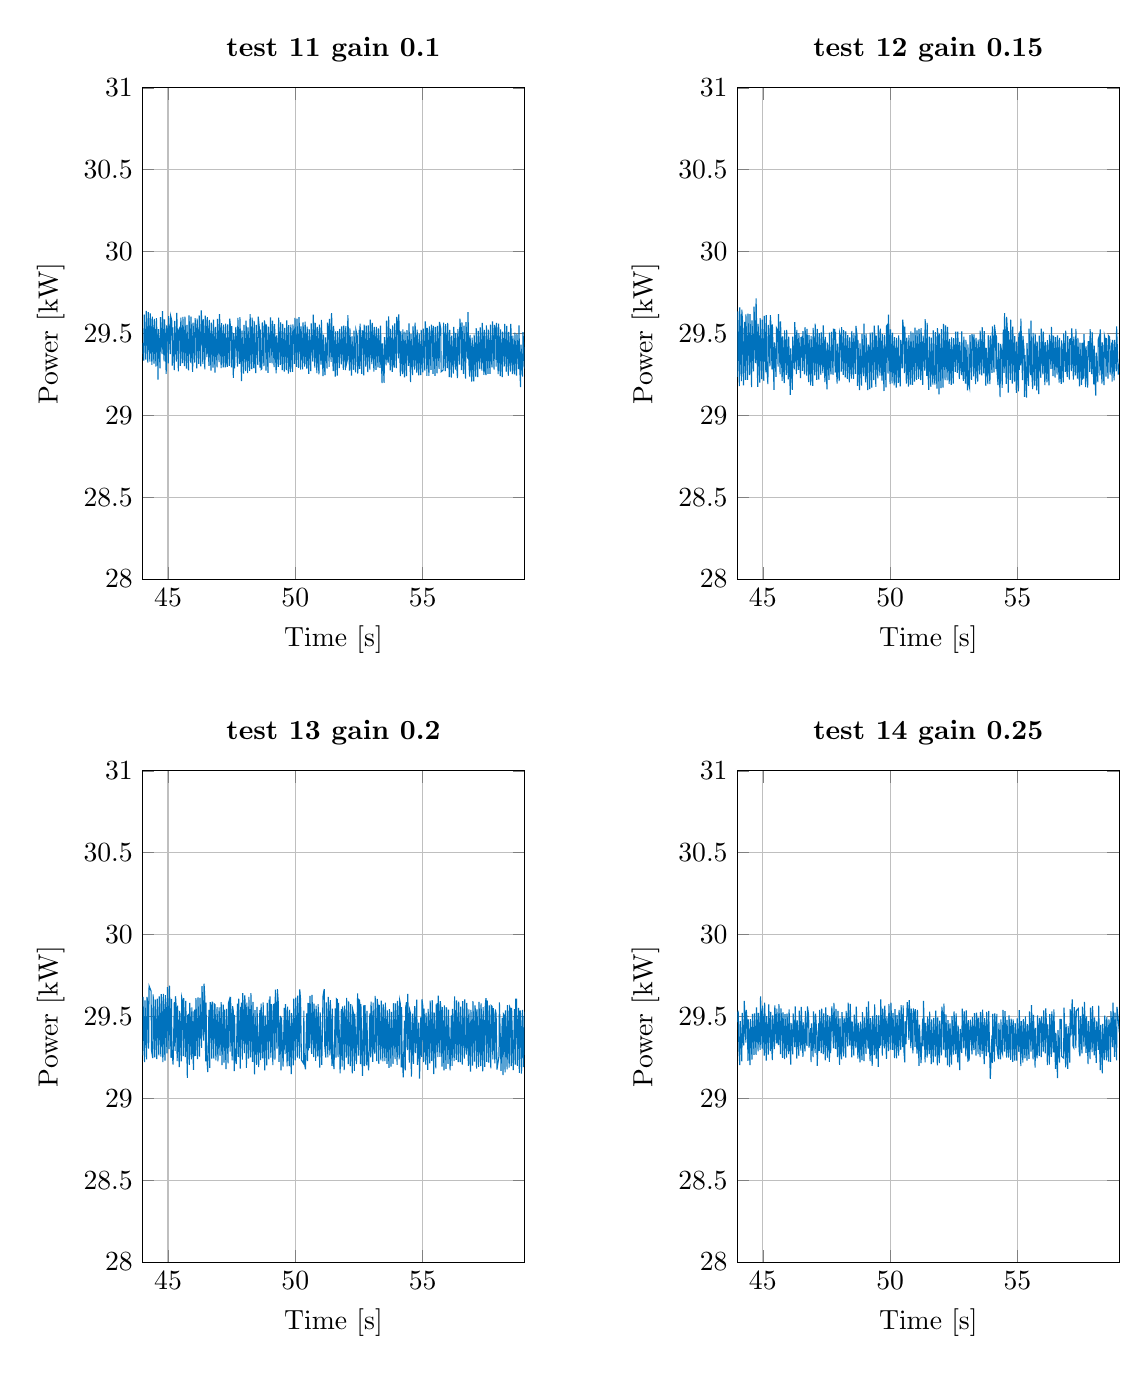
\begin{tikzpicture}

\begin{axis}[%
width=0.4\textwidth,
height=2.456in,
at={(1.026in,4.208in)},
scale only axis,
xmin=44,
xmax=59,
xlabel={Time [s]},
xmajorgrids,
ymin=28,
ymax=31,
ylabel={Power [kW]},
ymajorgrids,
axis background/.style={fill=white},
title style={font=\bfseries},
title={test 11 gain 0.1}
]
\addplot [color=mycolor1,solid,forget plot]
  table[row sep=crcr]{%
44	29.4420686313118\\
44.048	29.3343896078715\\
44.064	29.6158001455672\\
44.128	29.3407100501844\\
44.144	29.6376311648306\\
44.208	29.3213606341242\\
44.224	29.6308061562256\\
44.288	29.3287226242678\\
44.304	29.6229042765187\\
44.368	29.3081285789059\\
44.384	29.6027335850271\\
44.448	29.3159209944365\\
44.464	29.5885232520388\\
44.528	29.2983626335592\\
44.544	29.5940999330421\\
44.592	29.372567418678\\
44.608	29.2187207020092\\
44.624	29.5262685833224\\
44.688	29.2870023432478\\
44.704	29.5992721221852\\
44.768	29.3742253452181\\
44.784	29.6369781966536\\
44.816	29.4318830430937\\
44.848	29.3294199144766\\
44.864	29.5866384373771\\
44.928	29.2525682806497\\
44.944	29.5495512652029\\
44.992	29.4860146879361\\
45.008	29.317369840354\\
45.024	29.605205796073\\
45.088	29.3740758335877\\
45.104	29.6064675384365\\
45.152	29.5752614752973\\
45.168	29.3033706421226\\
45.184	29.5378740252297\\
45.248	29.2768592698802\\
45.264	29.5764926917497\\
45.328	29.32832361665\\
45.344	29.625950662763\\
45.408	29.2683746997774\\
45.424	29.5215192866496\\
45.472	29.5375867995139\\
45.488	29.3022145426906\\
45.504	29.5963702076373\\
45.568	29.3186588689051\\
45.584	29.6009938435632\\
45.648	29.3008613063311\\
45.664	29.6031398260931\\
45.728	29.2850462495867\\
45.744	29.5520500298386\\
45.808	29.2741648231249\\
45.824	29.6109524573689\\
45.888	29.3220620541214\\
45.904	29.6029636543553\\
45.936	29.38050460061\\
45.968	29.2658733393234\\
45.984	29.5657630790408\\
46.048	29.3218705648485\\
46.064	29.5935093510323\\
46.112	29.4731850185553\\
46.128	29.2869293803692\\
46.144	29.5904283102331\\
46.208	29.313838875327\\
46.224	29.6104503708362\\
46.288	29.298623685636\\
46.304	29.6409009526176\\
46.352	29.4836863887864\\
46.368	29.3142746246885\\
46.384	29.5867571645623\\
46.448	29.2802415789135\\
46.464	29.6094762402429\\
46.528	29.35596586833\\
46.544	29.5997662019529\\
46.608	29.3021996065567\\
46.624	29.582707511631\\
46.688	29.2727784481391\\
46.704	29.5655318615967\\
46.768	29.2917587014926\\
46.784	29.5852086312705\\
46.848	29.2608285356531\\
46.864	29.5409112041838\\
46.928	29.2934038330092\\
46.944	29.5885704419766\\
47.008	29.3252943805073\\
47.024	29.6187233344019\\
47.088	29.2884319702894\\
47.104	29.5636078920302\\
47.168	29.2926787050066\\
47.184	29.5540197552742\\
47.248	29.2923196876766\\
47.264	29.5594926237281\\
47.296	29.3340540249309\\
47.328	29.2962327261762\\
47.344	29.5551063047478\\
47.408	29.3022265268662\\
47.424	29.5900913847559\\
47.472	29.513440521347\\
47.488	29.2926683336891\\
47.504	29.5451296963282\\
47.568	29.2286955433445\\
47.584	29.502059744352\\
47.616	29.2867843451018\\
47.664	29.5401010036965\\
47.728	29.2976613601453\\
47.744	29.5948115571442\\
47.808	29.3138341665433\\
47.824	29.5992526721187\\
47.888	29.2090119744306\\
47.904	29.5180337240754\\
47.968	29.2545042721722\\
47.984	29.5523804991092\\
48.048	29.2699292481178\\
48.064	29.5789597832077\\
48.128	29.2585143847833\\
48.144	29.5366298916236\\
48.208	29.2718389083339\\
48.224	29.6186434239785\\
48.288	29.281926586792\\
48.304	29.596776872646\\
48.368	29.2881461693856\\
48.384	29.5770985605399\\
48.416	29.3479777404523\\
48.448	29.2585223955143\\
48.464	29.5518188789646\\
48.528	29.3079081134297\\
48.544	29.6022206077685\\
48.592	29.5274660354284\\
48.608	29.2921620168078\\
48.624	29.5239871871324\\
48.656	29.2801820819216\\
48.688	29.2855919287683\\
48.704	29.5676908198805\\
48.768	29.3002312001084\\
48.784	29.5794560020417\\
48.832	29.5302362553886\\
48.848	29.2735312993742\\
48.864	29.5559142224547\\
48.928	29.2589650902001\\
48.944	29.5420896368655\\
49.008	29.32064129668\\
49.024	29.5986973952683\\
49.088	29.3169832507176\\
49.104	29.5783800105176\\
49.168	29.294689573831\\
49.184	29.557145848462\\
49.248	29.2567942441381\\
49.264	29.4883986121614\\
49.328	29.296019894536\\
49.344	29.5970953178898\\
49.408	29.3082087335569\\
49.424	29.568442172763\\
49.488	29.2757890606816\\
49.504	29.5578102651561\\
49.568	29.2675864238439\\
49.584	29.5336976883686\\
49.648	29.2761040306643\\
49.664	29.5796181194604\\
49.728	29.2553296535973\\
49.744	29.5515642199602\\
49.776	29.3088290509179\\
49.808	29.2638250844792\\
49.824	29.5540640444827\\
49.888	29.2654337367647\\
49.904	29.5552206409881\\
49.952	29.4347106883175\\
49.968	29.3139194490089\\
49.984	29.5953631904551\\
50.048	29.2962036792834\\
50.064	29.5907507892205\\
50.128	29.2897109269613\\
50.144	29.5992433682848\\
50.192	29.4098358197205\\
50.208	29.2788399171571\\
50.224	29.543086310505\\
50.288	29.2807788928546\\
50.304	29.5669697652884\\
50.368	29.2979423644696\\
50.384	29.571696083248\\
50.448	29.2855634447884\\
50.464	29.5415802609181\\
50.528	29.2536572833084\\
50.544	29.526642261907\\
50.608	29.2705111494506\\
50.624	29.561782099311\\
50.688	29.3276748696342\\
50.704	29.6144472046945\\
50.768	29.2913421781915\\
50.784	29.5650490445994\\
50.848	29.2581621291327\\
50.864	29.5401046073323\\
50.928	29.2504249919803\\
50.944	29.5546637679552\\
51.008	29.3097711895513\\
51.024	29.5828105414871\\
51.088	29.2391371448774\\
51.104	29.4932534652415\\
51.136	29.3200229330523\\
51.168	29.2451156832768\\
51.184	29.47636121042\\
51.248	29.2860535988433\\
51.264	29.5663627074919\\
51.312	29.512282669845\\
51.328	29.2966390955234\\
51.344	29.5894084733161\\
51.408	29.3260269339092\\
51.424	29.6238215243169\\
51.488	29.269434917402\\
51.504	29.54656136258\\
51.568	29.2368554379912\\
51.584	29.5126697204576\\
51.648	29.2421679430167\\
51.664	29.5148256943628\\
51.728	29.2881036560551\\
51.744	29.5282805083768\\
51.808	29.3117364021196\\
51.824	29.5439076215226\\
51.888	29.2784795168248\\
51.904	29.5483449768277\\
51.968	29.2758271029439\\
51.984	29.5453686723623\\
52.016	29.3182668010762\\
52.048	29.3409179117936\\
52.064	29.6115916327278\\
52.128	29.2733402589082\\
52.144	29.5306799978524\\
52.208	29.2423374684843\\
52.224	29.4829181064535\\
52.288	29.2785366885008\\
52.304	29.5170960036759\\
52.368	29.2627357957673\\
52.384	29.5193069670064\\
52.432	29.4850593337498\\
52.448	29.2548104362442\\
52.496	29.3538075313201\\
52.512	29.5213046193323\\
52.528	29.2840192702022\\
52.544	29.560125303646\\
52.608	29.2539724544491\\
52.624	29.5162917451639\\
52.672	29.5129938252237\\
52.688	29.2440915134362\\
52.704	29.5545657592268\\
52.768	29.2978447053218\\
52.784	29.5484735877145\\
52.848	29.2641980378499\\
52.864	29.5495626750864\\
52.928	29.2794668310537\\
52.944	29.5846260994525\\
53.008	29.312417146679\\
53.024	29.5646018283204\\
53.088	29.2671098571877\\
53.104	29.5401818395818\\
53.168	29.2773464243369\\
53.184	29.5398831623092\\
53.248	29.2927357143766\\
53.264	29.5308789769811\\
53.328	29.2903208759242\\
53.344	29.5479213443326\\
53.408	29.197265064694\\
53.424	29.4386939953541\\
53.488	29.1976638127991\\
53.504	29.4769181703432\\
53.568	29.3049511575151\\
53.584	29.5786364245846\\
53.616	29.3627847102133\\
53.648	29.3196846003875\\
53.664	29.6048147398833\\
53.728	29.2739803989985\\
53.744	29.5278094945422\\
53.808	29.2658750497422\\
53.824	29.5495352288747\\
53.856	29.3201514012908\\
53.888	29.2913157648056\\
53.904	29.5621136822177\\
53.968	29.2880196321665\\
53.984	29.6014761484494\\
54.032	29.5353655417824\\
54.048	29.3479866458364\\
54.064	29.6163881080833\\
54.128	29.2396152794393\\
54.144	29.5149207188365\\
54.208	29.251151299195\\
54.224	29.5253778801714\\
54.288	29.2315260106896\\
54.304	29.5117674448358\\
54.368	29.2399088366028\\
54.384	29.5208719233893\\
54.448	29.302289450722\\
54.464	29.5613216820363\\
54.528	29.2029364230553\\
54.544	29.4954957190817\\
54.608	29.2455371961508\\
54.624	29.5435320051105\\
54.688	29.2797319282929\\
54.704	29.5662696132789\\
54.768	29.2611728900516\\
54.784	29.5228659555811\\
54.848	29.2436811657777\\
54.864	29.5003456819371\\
54.928	29.2462078789286\\
54.944	29.5213831037134\\
54.976	29.3383815370466\\
55.008	29.2629274708766\\
55.024	29.5297559166194\\
55.088	29.2728784253134\\
55.104	29.57370058137\\
55.152	29.4615683845007\\
55.168	29.2403396517443\\
55.184	29.5335063386757\\
55.248	29.241040573908\\
55.264	29.5434617476557\\
55.328	29.277874733195\\
55.344	29.554455226984\\
55.392	29.4751181221699\\
55.408	29.2529626713925\\
55.424	29.5468041078021\\
55.488	29.2407363355292\\
55.504	29.5398268480553\\
55.568	29.2569702496276\\
55.584	29.5464786127348\\
55.648	29.2843245200866\\
55.664	29.5706607637646\\
55.712	29.5298705467882\\
55.728	29.266414521063\\
55.808	29.2768037940012\\
55.824	29.5656857093991\\
55.888	29.2696450614396\\
55.904	29.5576185680591\\
55.968	29.2880408333427\\
55.984	29.5646065313254\\
56.048	29.2330940059076\\
56.064	29.5219522495561\\
56.128	29.2309110590447\\
56.144	29.4872270109408\\
56.208	29.2541701667215\\
56.224	29.5397276012038\\
56.288	29.2790548863171\\
56.304	29.5040727307433\\
56.336	29.320660674575\\
56.368	29.2277331583396\\
56.384	29.5271619133115\\
56.448	29.3099321789152\\
56.464	29.5904658696066\\
56.512	29.4789877941645\\
56.528	29.2766219678924\\
56.544	29.5684339013452\\
56.608	29.2534388552688\\
56.624	29.5471119397026\\
56.688	29.2242463969141\\
56.704	29.5685255837257\\
56.768	29.3463384458821\\
56.784	29.6305014820219\\
56.816	29.3267807798556\\
56.848	29.2366293186454\\
56.864	29.491218177616\\
56.928	29.2063894999814\\
56.944	29.473921909067\\
57.008	29.2071558587624\\
57.024	29.4923933136507\\
57.088	29.2368671469745\\
57.104	29.5325772135597\\
57.168	29.2332006586956\\
57.184	29.51585316193\\
57.248	29.2817925582689\\
57.264	29.5365147765399\\
57.328	29.2728136440206\\
57.344	29.5651086349785\\
57.408	29.2468588602678\\
57.424	29.5219588271355\\
57.456	29.2767461032088\\
57.488	29.246080776346\\
57.504	29.5496916861406\\
57.568	29.2539837699122\\
57.584	29.5238570973442\\
57.648	29.2527289077599\\
57.664	29.55390145755\\
57.696	29.3528368435991\\
57.728	29.2928374941704\\
57.744	29.5739610422259\\
57.808	29.2795220352382\\
57.824	29.552443065625\\
57.872	29.505407220236\\
57.888	29.2979439881885\\
57.904	29.564686032892\\
57.968	29.2515489294556\\
57.984	29.5599878389766\\
58.048	29.2393872686936\\
58.064	29.5245828432958\\
58.128	29.232817325329\\
58.144	29.5117259671454\\
58.208	29.2984217714542\\
58.224	29.5580200771935\\
58.288	29.2662999092999\\
58.304	29.5456162775393\\
58.368	29.2418522056443\\
58.384	29.5102131954606\\
58.448	29.2666400770418\\
58.464	29.558163292968\\
58.528	29.2515070024044\\
58.544	29.4863085025716\\
58.608	29.2496649370278\\
58.624	29.5052073021487\\
58.688	29.2431097829002\\
58.704	29.4963484088734\\
58.768	29.2821854632837\\
58.784	29.5490535665863\\
58.816	29.2873349433909\\
58.848	29.1729518274999\\
58.864	29.4321001864769\\
58.928	29.2369322085582\\
58.944	29.5085236787105\\
59.008	29.2851796650143\\
};
\end{axis}

\begin{axis}[%
width=0.4\textwidth,
height=2.456in,
at={(4in,4.208in)},
scale only axis,
xmin=44,
xmax=59,
xlabel={Time [s]},
xmajorgrids,
ymin=28,
ymax=31,
ylabel={Power [kW]},
ymajorgrids,
axis background/.style={fill=white},
title style={font=\bfseries},
title={test 12  gain 0.15}
]
\addplot [color=mycolor1,solid,forget plot]
  table[row sep=crcr]{%
44	29.2354896011076\\
44.016	29.6349815294779\\
44.08	29.1780735601847\\
44.096	29.6590677798893\\
44.16	29.2088027541431\\
44.176	29.6453243274993\\
44.208	29.5610029840513\\
44.24	29.1828334528868\\
44.288	29.5713326743684\\
44.32	29.2170689728208\\
44.336	29.6160841419116\\
44.4	29.2173578189126\\
44.416	29.6216524960193\\
44.48	29.2454452231944\\
44.496	29.6180732364441\\
44.56	29.1727409916738\\
44.576	29.5798290607628\\
44.64	29.2686034842653\\
44.656	29.6634093673792\\
44.72	29.3195122972223\\
44.736	29.7140106838235\\
44.8	29.1746207449822\\
44.816	29.558232358\\
44.88	29.2003074107644\\
44.896	29.5930213653859\\
44.96	29.220713510897\\
44.976	29.584386139896\\
45.04	29.2104210658648\\
45.056	29.6080137101032\\
45.12	29.2632178647556\\
45.136	29.6116962665291\\
45.152	29.3150309744516\\
45.2	29.1909551220164\\
45.216	29.5524911368225\\
45.28	29.2990675702345\\
45.296	29.6118054529547\\
45.328	29.5297267693732\\
45.36	29.281049300728\\
45.376	29.5549734918105\\
45.44	29.1560448081586\\
45.456	29.445158557608\\
45.52	29.2352075982332\\
45.536	29.5330025588231\\
45.584	29.5163592489433\\
45.6	29.2975574652578\\
45.616	29.6174911579789\\
45.68	29.2510113673102\\
45.696	29.574356002236\\
45.76	29.21028646966\\
45.776	29.4814717222096\\
45.84	29.1961551680583\\
45.856	29.5181223793641\\
45.92	29.2472555944257\\
45.936	29.5223720241275\\
46	29.2196472072024\\
46.016	29.4809409774924\\
46.08	29.12538665342\\
46.096	29.4095222388008\\
46.16	29.155105777251\\
46.176	29.4806659089715\\
46.24	29.2810909930331\\
46.256	29.5695017619998\\
46.32	29.2517212903468\\
46.336	29.5214426012867\\
46.4	29.2774167576722\\
46.416	29.5013088875685\\
46.48	29.2277167054589\\
46.496	29.4773480060941\\
46.512	29.3524498066351\\
46.544	29.4846512903169\\
46.56	29.2718157428888\\
46.576	29.5143582967914\\
46.64	29.2505384971599\\
46.656	29.5377925482332\\
46.704	29.4249498370896\\
46.72	29.241924364103\\
46.736	29.5275856014169\\
46.8	29.2025610174032\\
46.816	29.4907076546142\\
46.88	29.1824628087884\\
46.896	29.4845622786531\\
46.96	29.1795418584376\\
46.976	29.5335589957263\\
47.04	29.2442972557972\\
47.056	29.5605911241239\\
47.12	29.2167995581606\\
47.136	29.5276569227323\\
47.2	29.2181693058409\\
47.216	29.50271753221\\
47.28	29.2478243289659\\
47.296	29.5072777518166\\
47.36	29.2581687113991\\
47.376	29.5492485924979\\
47.44	29.2022959273133\\
47.456	29.4787606944033\\
47.52	29.1589715642155\\
47.536	29.4441235623949\\
47.6	29.2168584094622\\
47.616	29.5056424647346\\
47.632	29.3466276210118\\
47.68	29.2500838357491\\
47.696	29.5103896932793\\
47.76	29.2479517325283\\
47.776	29.5259954139324\\
47.824	29.5238835600605\\
47.84	29.261531623493\\
47.856	29.5089816155652\\
47.888	29.2902697854574\\
47.92	29.1941109798783\\
47.936	29.4373832518033\\
48	29.2092389834003\\
48.016	29.5070222776475\\
48.064	29.4754018731906\\
48.08	29.2671161144113\\
48.096	29.5383348785986\\
48.16	29.2473171920165\\
48.176	29.5198873107676\\
48.24	29.2318889267621\\
48.256	29.5127074505337\\
48.32	29.2221003331945\\
48.336	29.4905602504426\\
48.4	29.2019449194541\\
48.416	29.4756955605797\\
48.48	29.2237417809411\\
48.496	29.5150347350267\\
48.56	29.2220664574032\\
48.576	29.5035176322093\\
48.64	29.2527208450217\\
48.656	29.5467572652567\\
48.704	29.486866172491\\
48.72	29.1801832522219\\
48.736	29.4609738603301\\
48.8	29.1533599982466\\
48.816	29.4392863152142\\
48.88	29.1809782950955\\
48.896	29.4970660479599\\
48.96	29.2401481821806\\
48.976	29.5594049152132\\
48.992	29.3842306016614\\
49.04	29.2020430454146\\
49.056	29.4987638019965\\
49.12	29.1539985626852\\
49.136	29.4329372772638\\
49.184	29.3781244520496\\
49.2	29.1600433985565\\
49.216	29.5053094564094\\
49.28	29.169694607181\\
49.296	29.5069065016345\\
49.36	29.2151067797348\\
49.376	29.5478578278006\\
49.408	29.4590772443221\\
49.44	29.174235100312\\
49.456	29.4865808543287\\
49.52	29.2252093962139\\
49.536	29.54982531218\\
49.6	29.242087172824\\
49.616	29.5297119211111\\
49.68	29.2118873707948\\
49.696	29.4969280290385\\
49.76	29.1487254417258\\
49.776	29.4911328743816\\
49.84	29.1709108168548\\
49.856	29.5450709203054\\
49.888	29.5518627812357\\
49.92	29.2550190455546\\
49.936	29.6150581304273\\
50	29.1908418282569\\
50.016	29.5246394524625\\
50.08	29.1945600714122\\
50.096	29.504331341741\\
50.16	29.1831751286514\\
50.176	29.4783107785977\\
50.24	29.1700250719001\\
50.256	29.4729615915095\\
50.32	29.1984039667538\\
50.336	29.4889628364855\\
50.352	29.3137747986415\\
50.4	29.1771618556767\\
50.416	29.4607607165377\\
50.48	29.2868374144172\\
50.496	29.5842483375049\\
50.544	29.48679255561\\
50.56	29.2583188883301\\
50.576	29.5422124707915\\
50.64	29.1933187826762\\
50.656	29.4751352649262\\
50.72	29.1749920088917\\
50.736	29.4899605434264\\
50.8	29.186938463144\\
50.816	29.5129519955147\\
50.88	29.1856090342959\\
50.896	29.5058071062135\\
50.96	29.2053233024698\\
50.976	29.5350863040784\\
51.04	29.2164124469078\\
51.056	29.5185289802585\\
51.12	29.2224726493189\\
51.136	29.5274498711785\\
51.2	29.2154001530401\\
51.216	29.5324765345807\\
51.28	29.1864569973507\\
51.296	29.4864876723333\\
51.36	29.2726114881186\\
51.376	29.5882672609425\\
51.44	29.2407270183009\\
51.456	29.5648582224983\\
51.472	29.3124617972219\\
51.52	29.1549303446027\\
51.536	29.4801828668312\\
51.6	29.1735341970065\\
51.616	29.4742175540929\\
51.68	29.1875167596058\\
51.696	29.5195356289098\\
51.712	29.3056247420188\\
51.76	29.18763459659\\
51.776	29.5084221032333\\
51.84	29.162491285631\\
51.856	29.5321094877075\\
51.888	29.4719852197657\\
51.92	29.1281081618642\\
51.936	29.4992968537176\\
52	29.1668743168099\\
52.016	29.5260910510576\\
52.08	29.1693863112619\\
52.096	29.5587701288369\\
52.16	29.2154849068392\\
52.176	29.549558783813\\
52.24	29.2141715409715\\
52.256	29.5409512876241\\
52.32	29.1921586100194\\
52.336	29.4675706562618\\
52.4	29.1858308329815\\
52.416	29.4768248391976\\
52.48	29.1938762686715\\
52.496	29.4718148862805\\
52.56	29.2662011019736\\
52.576	29.5113531492838\\
52.64	29.2598170008455\\
52.656	29.511216666364\\
52.72	29.2220112710088\\
52.736	29.4487052951591\\
52.8	29.2457170206973\\
52.816	29.5132390145019\\
52.832	29.318577799215\\
52.88	29.2104662624829\\
52.896	29.4810134324532\\
52.96	29.1937264000017\\
52.976	29.4614751864268\\
53.04	29.1519584326859\\
53.056	29.4327296369083\\
53.072	29.2065296793494\\
53.12	29.1703326088334\\
53.136	29.4891867241861\\
53.2	29.2171760084222\\
53.216	29.4954204035081\\
53.264	29.4439405546703\\
53.28	29.2378711840586\\
53.296	29.4951325684922\\
53.36	29.1903152272931\\
53.376	29.4727270457005\\
53.44	29.2062958913233\\
53.456	29.4626279382237\\
53.52	29.2504585229259\\
53.536	29.5171920905095\\
53.6	29.2445280716867\\
53.616	29.5392539302353\\
53.68	29.2559389735317\\
53.696	29.5148860563411\\
53.76	29.1794745959419\\
53.776	29.4125047734591\\
53.84	29.1904826976476\\
53.856	29.4890417149605\\
53.92	29.1913936706942\\
53.936	29.4861726755532\\
54	29.2598320003077\\
54.016	29.5438142754362\\
54.08	29.2619783681502\\
54.096	29.5530187304401\\
54.144	29.4944062806476\\
54.16	29.2833549784342\\
54.176	29.4888182762809\\
54.192	29.2863970310841\\
54.24	29.1840656319419\\
54.256	29.4427721092313\\
54.32	29.1118499293733\\
54.336	29.4367118795074\\
54.384	29.3881525115516\\
54.4	29.1678752094466\\
54.448	29.5227271978482\\
54.48	29.2601182066209\\
54.496	29.6236619648991\\
54.56	29.1924725065879\\
54.576	29.6008421572485\\
54.608	29.5121529779297\\
54.64	29.1392027144245\\
54.656	29.514488102461\\
54.72	29.2166623745199\\
54.736	29.5843747371018\\
54.8	29.1941926228659\\
54.816	29.5417443979713\\
54.88	29.2065822963999\\
54.896	29.4841892963577\\
54.96	29.1375828381121\\
54.976	29.4503115433216\\
55.04	29.1461543090015\\
55.056	29.5036594867331\\
55.072	29.2772367493822\\
55.104	29.5125982301325\\
55.12	29.3047215702603\\
55.136	29.5912222954264\\
55.2	29.2144968798145\\
55.216	29.4845217143381\\
55.264	29.3933318863511\\
55.28	29.1127566531365\\
55.296	29.3684154238601\\
55.36	29.1079628185831\\
55.376	29.4407554293799\\
55.44	29.1794006056615\\
55.456	29.5299930274363\\
55.52	29.2459361067561\\
55.536	29.5787084095614\\
55.552	29.3006255579945\\
55.6	29.1598966715595\\
55.616	29.5039819956337\\
55.68	29.1814905890492\\
55.696	29.4989922286389\\
55.728	29.3897493857272\\
55.76	29.1521036169628\\
55.776	29.4502832234515\\
55.84	29.1292746017857\\
55.856	29.486329042793\\
55.92	29.2294839169927\\
55.936	29.5297419678404\\
56	29.2501047729992\\
56.016	29.5111281718112\\
56.08	29.1839985761352\\
56.096	29.4472111579873\\
56.16	29.2020979719008\\
56.176	29.4586611393143\\
56.24	29.1828187396741\\
56.256	29.4935402918712\\
56.32	29.2838432830042\\
56.336	29.5406282064031\\
56.4	29.2401025158791\\
56.416	29.4869164829258\\
56.48	29.2310176798545\\
56.496	29.4772105430221\\
56.56	29.2486170369052\\
56.576	29.4886511147299\\
56.64	29.1996852584118\\
56.656	29.4724566066086\\
56.672	29.2875483030935\\
56.72	29.1928496792694\\
56.736	29.4574960670185\\
56.8	29.2017744984943\\
56.816	29.5010929356307\\
56.88	29.265339937956\\
56.896	29.5177861821508\\
56.912	29.3207355071472\\
56.96	29.2343140434255\\
56.976	29.4837012633192\\
57.04	29.2187649616052\\
57.056	29.4632061124961\\
57.104	29.4689772911954\\
57.12	29.269532226107\\
57.136	29.5313573348865\\
57.2	29.2180579671608\\
57.216	29.4803299085605\\
57.28	29.2442609489061\\
57.296	29.528449369118\\
57.36	29.2242512367605\\
57.376	29.4725533551405\\
57.44	29.1763764945606\\
57.456	29.4437235364867\\
57.52	29.186180097562\\
57.536	29.4427400455437\\
57.552	29.2179350824113\\
57.584	29.4442115138226\\
57.6	29.2238289161259\\
57.616	29.4955077598567\\
57.68	29.1730972224457\\
57.696	29.4211787876807\\
57.76	29.1698852171342\\
57.776	29.4492514705466\\
57.824	29.4498471448244\\
57.84	29.2659463215264\\
57.856	29.5270129852665\\
57.92	29.2518838841605\\
57.936	29.5077102861133\\
58	29.1888081167533\\
58.016	29.4251509072244\\
58.048	29.2190697223194\\
58.08	29.1198648236896\\
58.096	29.383523391406\\
58.16	29.2036571907138\\
58.176	29.4631686002556\\
58.224	29.4871145987148\\
58.24	29.2440832854667\\
58.256	29.5243965809857\\
58.32	29.194232768069\\
58.336	29.4451182463636\\
58.4	29.1844940055813\\
58.416	29.4876782359608\\
58.464	29.4545718832697\\
58.48	29.2362479973236\\
58.496	29.4718497940499\\
58.56	29.2244675675042\\
58.576	29.4866855638197\\
58.624	29.4777461923622\\
58.64	29.2493707474116\\
58.704	29.4438775478786\\
58.72	29.2056527242017\\
58.736	29.4606063717443\\
58.8	29.2139638793814\\
58.816	29.461328019459\\
58.88	29.2685183285291\\
58.896	29.5430592948945\\
58.96	29.2490098870287\\
59.008	29.3203655992174\\
};
\end{axis}

\begin{axis}[%
width=0.4\textwidth,
height=2.456in,
at={(1.026in,0.793in)},
scale only axis,
xmin=44,
xmax=59,
xlabel={Time [s]},
xmajorgrids,
ymin=28,
ymax=31,
ylabel={Power [kW]},
ymajorgrids,
axis background/.style={fill=white},
title style={font=\bfseries},
title={test 13  gain 0.2}
]
\addplot [color=mycolor1,solid,forget plot]
  table[row sep=crcr]{%
44	29.2618643203586\\
44.016	29.6195084950626\\
44.08	29.2213002546617\\
44.096	29.5983687549621\\
44.16	29.2380916264961\\
44.176	29.6195553367821\\
44.208	29.5720542417704\\
44.24	29.303322687237\\
44.256	29.6872106125649\\
44.336	29.6547256890066\\
44.352	29.2927805775486\\
44.4	29.2454467883537\\
44.416	29.6343964433038\\
44.48	29.2507592742143\\
44.496	29.6038670538354\\
44.56	29.2401815255611\\
44.576	29.6081692638355\\
44.64	29.2622936559152\\
44.656	29.6228220997037\\
44.72	29.2541106449184\\
44.736	29.636450890969\\
44.8	29.2208632993081\\
44.816	29.637878008161\\
44.88	29.2302403817606\\
44.896	29.6301562671479\\
44.96	29.2746184114174\\
44.976	29.6797843186009\\
45.04	29.3010927331881\\
45.056	29.6883602365267\\
45.12	29.2479195548576\\
45.136	29.6068148603073\\
45.152	29.301736172864\\
45.2	29.2057868595124\\
45.248	29.587212833022\\
45.28	29.2899439041826\\
45.296	29.6233931933104\\
45.328	29.5425712430485\\
45.36	29.2276163561078\\
45.376	29.5655531311807\\
45.44	29.1902751728761\\
45.456	29.5343084374894\\
45.52	29.2261869442173\\
45.536	29.6175846806785\\
45.568	29.5946276439815\\
45.6	29.2575612045121\\
45.616	29.6118272485706\\
45.68	29.2511572463873\\
45.696	29.5950284403254\\
45.76	29.1256699353868\\
45.776	29.505997715998\\
45.808	29.5113604815212\\
45.84	29.2047642297329\\
45.856	29.5832368912069\\
45.92	29.2380654111815\\
45.936	29.555897776472\\
46	29.1740373619606\\
46.016	29.5318109015713\\
46.032	29.2576882822455\\
46.048	29.5411880760683\\
46.08	29.2598331901668\\
46.096	29.611311399475\\
46.16	29.2398516055996\\
46.176	29.6158347457995\\
46.24	29.2545662681111\\
46.256	29.6142494675056\\
46.32	29.307813167222\\
46.336	29.6845425186481\\
46.4	29.3521964361871\\
46.416	29.7002089090406\\
46.448	29.6075526585224\\
46.48	29.2263983497921\\
46.496	29.5849176520307\\
46.512	29.2796597690735\\
46.56	29.1609381164561\\
46.608	29.5406942308045\\
46.64	29.1860666376868\\
46.656	29.5874336693249\\
46.688	29.5612978715561\\
46.72	29.2428102510567\\
46.736	29.591306553288\\
46.8	29.2422448852286\\
46.816	29.5769512964816\\
46.848	29.5715497526895\\
46.88	29.2321536683142\\
46.928	29.5563207934369\\
46.96	29.225938709543\\
47.008	29.5548626675201\\
47.04	29.2601798085177\\
47.088	29.5870386433382\\
47.12	29.2021590889654\\
47.168	29.5717705601899\\
47.2	29.2180450574257\\
47.216	29.5424243953001\\
47.28	29.1778979613544\\
47.296	29.5457505134057\\
47.36	29.2135853164157\\
47.376	29.5816541244717\\
47.408	29.5995777691848\\
47.44	29.2859274428892\\
47.456	29.6200984216174\\
47.52	29.2318503838047\\
47.536	29.5632469841007\\
47.568	29.5293978491003\\
47.6	29.165800825963\\
47.616	29.509739415911\\
47.632	29.2596805248822\\
47.68	29.2098541355352\\
47.728	29.579070926234\\
47.76	29.2533236871064\\
47.776	29.6092501575745\\
47.84	29.1807979673508\\
47.856	29.5589850494236\\
47.872	29.3593635124883\\
47.888	29.5845791897055\\
47.92	29.2370697000537\\
47.936	29.642525948174\\
48	29.2764131767677\\
48.016	29.6286777627321\\
48.048	29.5134985098503\\
48.08	29.1862416735911\\
48.096	29.5841702796599\\
48.16	29.2420235763807\\
48.176	29.6194849708507\\
48.24	29.2498400119346\\
48.256	29.6425737649447\\
48.32	29.2233831134159\\
48.336	29.5885573228907\\
48.4	29.1465525884225\\
48.416	29.5394101218623\\
48.48	29.2045306184483\\
48.496	29.5587379698712\\
48.56	29.1900352402955\\
48.608	29.5390265073581\\
48.64	29.2332857610019\\
48.656	29.578871967213\\
48.72	29.2442018645399\\
48.736	29.5856825411632\\
48.8	29.1710253265135\\
48.816	29.5060535116898\\
48.88	29.2015510325193\\
48.896	29.5830815604736\\
48.96	29.2374694333086\\
48.976	29.6027989275207\\
48.992	29.3502688151919\\
49.008	29.6221443105814\\
49.04	29.248675199778\\
49.056	29.575569083208\\
49.12	29.202397621062\\
49.136	29.5714249261527\\
49.168	29.5748385227533\\
49.2	29.2360506135107\\
49.216	29.6644437902542\\
49.28	29.3043512647536\\
49.296	29.6670980822181\\
49.328	29.5928961844666\\
49.36	29.2229754339298\\
49.408	29.5032388545433\\
49.44	29.1703003193382\\
49.456	29.4944826242134\\
49.52	29.1932196887198\\
49.568	29.5531885947999\\
49.6	29.2694614045224\\
49.616	29.57587605797\\
49.68	29.1948777958202\\
49.696	29.5607202933248\\
49.76	29.196216242848\\
49.776	29.5409869272347\\
49.84	29.1476292500111\\
49.856	29.5203473553225\\
49.92	29.2021299022045\\
49.936	29.6095674513386\\
50	29.232402075755\\
50.016	29.6148193607551\\
50.08	29.2483483729656\\
50.096	29.6277116849987\\
50.16	29.2427252541384\\
50.176	29.6651063191924\\
50.208	29.5990121407061\\
50.24	29.2329408608591\\
50.32	29.2137894108882\\
50.336	29.5360516166734\\
50.352	29.2203415088799\\
50.4	29.1771145835586\\
50.448	29.518985681799\\
50.48	29.2277358781698\\
50.496	29.5836411910467\\
50.512	29.2930968301284\\
50.528	29.5818593506389\\
50.56	29.306063960695\\
50.576	29.6252652431892\\
50.64	29.2712644302178\\
50.656	29.6312630679314\\
50.72	29.2518103048336\\
50.736	29.5790131521085\\
50.8	29.2285335115242\\
50.816	29.5666718525253\\
50.88	29.2570543981932\\
50.896	29.5756442728999\\
50.96	29.18773568424\\
50.976	29.5248271960233\\
51.04	29.2039144422874\\
51.088	29.6244843429078\\
51.136	29.6673238728896\\
51.152	29.3267898615423\\
51.2	29.2482252045561\\
51.216	29.5855051618072\\
51.28	29.2504010801773\\
51.296	29.6195938171816\\
51.36	29.2631468623253\\
51.376	29.6001573352272\\
51.44	29.1980746435634\\
51.456	29.5474052156432\\
51.472	29.2689174974857\\
51.52	29.1783006325954\\
51.568	29.5487660800106\\
51.6	29.2480085896898\\
51.616	29.608159709939\\
51.648	29.6033522143483\\
51.68	29.2512953715585\\
51.696	29.5825082286096\\
51.744	29.3031922171481\\
51.76	29.1531605664857\\
51.808	29.5440985350156\\
51.84	29.1940395482819\\
51.856	29.5620507528711\\
51.888	29.5047528779063\\
51.92	29.1724783708588\\
51.936	29.565599325565\\
52	29.2492156345383\\
52.016	29.6136340963284\\
52.08	29.2087267534638\\
52.096	29.5927468655503\\
52.16	29.1966936128422\\
52.176	29.5756779003851\\
52.24	29.1520761167908\\
52.256	29.5410298688729\\
52.288	29.5182447967337\\
52.32	29.1680870242909\\
52.336	29.5160866422456\\
52.4	29.2095656408614\\
52.448	29.641132121746\\
52.48	29.2607145750631\\
52.496	29.6026670962955\\
52.528	29.5991973620947\\
52.56	29.2093262321904\\
52.576	29.5752941494001\\
52.64	29.1371335951254\\
52.688	29.5678964610953\\
52.72	29.1971082554732\\
52.736	29.5697976594045\\
52.8	29.2019174693939\\
52.816	29.533901647474\\
52.832	29.2844994764327\\
52.88	29.1704280180188\\
52.928	29.5192799498269\\
52.96	29.2507057494248\\
52.976	29.5898792664006\\
53.04	29.2227960307625\\
53.056	29.5845104857313\\
53.072	29.3455490762095\\
53.12	29.2738013564979\\
53.136	29.6256352156597\\
53.2	29.2269792003968\\
53.216	29.6066611044229\\
53.248	29.5582953193729\\
53.28	29.2107185302969\\
53.296	29.5703387102471\\
53.36	29.2324356207704\\
53.376	29.5972811744792\\
53.44	29.2258053335195\\
53.456	29.5733182871761\\
53.52	29.227494477796\\
53.536	29.5840103193661\\
53.6	29.210556389756\\
53.616	29.5371991535561\\
53.68	29.1857262731566\\
53.696	29.5445641909978\\
53.76	29.193467842442\\
53.776	29.5281667164528\\
53.84	29.2101105838032\\
53.856	29.5807019942912\\
53.92	29.239664477956\\
53.936	29.57941084082\\
54	29.2038209452393\\
54.016	29.5949855596372\\
54.08	29.2373962522843\\
54.096	29.600656999614\\
54.128	29.5762675278396\\
54.16	29.1889459543159\\
54.176	29.5565808356828\\
54.192	29.2911012421436\\
54.24	29.1276917261928\\
54.288	29.4750518223705\\
54.32	29.1707062815445\\
54.336	29.555487870122\\
54.368	29.5874992983406\\
54.4	29.2947582268754\\
54.416	29.6384512545871\\
54.48	29.2181417323259\\
54.496	29.5368612042333\\
54.528	29.5162567283119\\
54.56	29.1327037705756\\
54.608	29.517792431402\\
54.64	29.2104177873518\\
54.688	29.5638609912078\\
54.72	29.2757894728386\\
54.768	29.603061552776\\
54.8	29.2042735989482\\
54.848	29.462310867448\\
54.88	29.1207962477195\\
54.928	29.4944678595283\\
54.96	29.2528347243514\\
54.976	29.6048493130274\\
55.008	29.5658153720853\\
55.04	29.221890865907\\
55.056	29.5485731199146\\
55.12	29.2064159598203\\
55.136	29.521353622942\\
55.2	29.1741834030679\\
55.216	29.5458937344043\\
55.28	29.214073544248\\
55.296	29.5972596881845\\
55.36	29.229627993432\\
55.376	29.6003901076358\\
55.44	29.1484949616279\\
55.456	29.5237124046099\\
55.52	29.1835380009832\\
55.536	29.5744649393179\\
55.552	29.3249848099606\\
55.568	29.5818922145779\\
55.6	29.251597407559\\
55.616	29.6279212369617\\
55.68	29.2534214961709\\
55.696	29.5937164996023\\
55.728	29.5227095311995\\
55.76	29.1932077001394\\
55.776	29.5564218113961\\
55.84	29.1713653680772\\
55.856	29.567628083623\\
55.92	29.1795523665094\\
55.936	29.5562316727196\\
56	29.2099461853827\\
56.016	29.5415794210751\\
56.08	29.1707454589952\\
56.128	29.5064675945243\\
56.16	29.1976782059998\\
56.176	29.546582149167\\
56.24	29.2273095758349\\
56.256	29.6232485957732\\
56.32	29.235017233314\\
56.336	29.5989404520582\\
56.4	29.2209100323805\\
56.416	29.5911119473125\\
56.48	29.2210177312732\\
56.496	29.5606974221232\\
56.56	29.2052407533097\\
56.576	29.5938050815628\\
56.64	29.2423490400962\\
56.656	29.603954991956\\
56.672	29.356187068074\\
56.72	29.2675032011446\\
56.736	29.5829735417236\\
56.8	29.1981147467131\\
56.816	29.5437938864784\\
56.88	29.1634647363356\\
56.896	29.5399067872357\\
56.944	29.3089462230198\\
56.96	29.1991582139405\\
56.976	29.5943786213905\\
57.04	29.2246056415879\\
57.056	29.5679207529783\\
57.088	29.5056172783737\\
57.12	29.1813116233646\\
57.136	29.543635061698\\
57.2	29.1919422890209\\
57.216	29.5887926894012\\
57.28	29.1961745307684\\
57.296	29.5797529871837\\
57.36	29.1647477638249\\
57.376	29.5563311625898\\
57.44	29.1921139085378\\
57.456	29.5509092407838\\
57.488	29.6121573854925\\
57.52	29.2230278458768\\
57.536	29.598924935965\\
57.6	29.2178282499508\\
57.616	29.5674272554159\\
57.68	29.1833881154121\\
57.696	29.56667149632\\
57.728	29.5615152188564\\
57.76	29.2384972576418\\
57.776	29.5503218503674\\
57.84	29.2142742093412\\
57.856	29.5424875909541\\
57.888	29.514781473621\\
57.92	29.17516761524\\
58	29.258676241803\\
58.016	29.5857857543245\\
58.064	29.2997486105474\\
58.08	29.168076497963\\
58.128	29.491869530039\\
58.16	29.1416700336339\\
58.176	29.5145740809821\\
58.208	29.5058906716186\\
58.24	29.1588770592526\\
58.256	29.5365175207574\\
58.32	29.17659374327\\
58.336	29.5691871768794\\
58.4	29.1877175488863\\
58.416	29.5593765375111\\
58.448	29.5475770264068\\
58.48	29.1961738626093\\
58.496	29.5527391398043\\
58.56	29.1718209791178\\
58.608	29.5444230699907\\
58.64	29.2058641089916\\
58.656	29.6058887082102\\
58.688	29.6059674722977\\
58.72	29.1981607243534\\
58.768	29.5519731625312\\
58.8	29.1549825734294\\
58.816	29.5327650052699\\
58.848	29.5331422138743\\
58.88	29.1507454388256\\
58.928	29.5399996017325\\
58.96	29.1904767290779\\
59.008	29.5290080542657\\
};
\end{axis}

\begin{axis}[%
width=0.4\textwidth,
height=2.456in,
at={(4in,0.793in)},
scale only axis,
xmin=44,
xmax=59,
xlabel={Time [s]},
xmajorgrids,
ymin=28,
ymax=31,
ylabel={Power [kW]},
ymajorgrids,
axis background/.style={fill=white},
title style={font=\bfseries},
title={test 14  gain 0.25}
]
\addplot [color=mycolor1,solid,forget plot]
  table[row sep=crcr]{%
44	29.4660891969925\\
44.032	29.5357815809023\\
44.064	29.2942895769538\\
44.096	29.2028389022579\\
44.112	29.4713019618038\\
44.176	29.2256097219192\\
44.192	29.5218523713626\\
44.224	29.3668419300147\\
44.256	29.3228776394523\\
44.272	29.5955810949925\\
44.336	29.3410393373158\\
44.352	29.5401568362132\\
44.4	29.4379623158044\\
44.416	29.229139310294\\
44.432	29.48143735071\\
44.496	29.2029416520345\\
44.512	29.4830981227037\\
44.576	29.237256425695\\
44.592	29.5163433985592\\
44.656	29.2659959406349\\
44.672	29.5185641262965\\
44.736	29.2660263587302\\
44.752	29.5548557975583\\
44.816	29.2872218712879\\
44.832	29.5223901466985\\
44.896	29.2962357622949\\
44.912	29.6228756990621\\
44.976	29.3035134416154\\
44.992	29.5666330057321\\
45.056	29.2610118165813\\
45.072	29.5841230338107\\
45.136	29.2300314009176\\
45.152	29.5020019619658\\
45.216	29.2672088809901\\
45.232	29.5737635713283\\
45.296	29.2881744938304\\
45.312	29.5280477236627\\
45.344	29.3294719177584\\
45.376	29.23396155102\\
45.392	29.5060640610191\\
45.456	29.3010554208063\\
45.472	29.5675565829014\\
45.536	29.3356378727169\\
45.552	29.547298397442\\
45.584	29.352137617525\\
45.616	29.3259431323701\\
45.632	29.5750072853005\\
45.696	29.2703217578034\\
45.712	29.5489092382944\\
45.76	29.409886302454\\
45.776	29.2466252376014\\
45.792	29.5247422397312\\
45.856	29.2401372150657\\
45.872	29.513698960846\\
45.936	29.2494823943234\\
45.952	29.5177576016783\\
46.016	29.2706947880766\\
46.032	29.5432650369002\\
46.096	29.205541861472\\
46.112	29.4587747484118\\
46.176	29.2689122304548\\
46.192	29.5186223120878\\
46.256	29.3122805700184\\
46.272	29.5610862384695\\
46.336	29.2420787166078\\
46.352	29.4766188341074\\
46.416	29.2601281833823\\
46.432	29.5352826409129\\
46.496	29.2915049482115\\
46.512	29.5578312806539\\
46.576	29.2536535099759\\
46.592	29.4633136446436\\
46.656	29.2864928272289\\
46.672	29.5339697787288\\
46.704	29.352112032882\\
46.736	29.3210040037946\\
46.752	29.5607757112102\\
46.8	29.5097912390543\\
46.816	29.3094217803901\\
46.88	29.4284702193393\\
46.896	29.2210508113302\\
46.912	29.4579004378984\\
46.976	29.2514319697715\\
46.992	29.5304705840891\\
47.056	29.2763468697306\\
47.072	29.516704509769\\
47.12	29.3985425488306\\
47.136	29.1979872113835\\
47.2	29.4591516209731\\
47.216	29.2900039826579\\
47.232	29.539582393035\\
47.296	29.2769439876109\\
47.312	29.5474170068158\\
47.376	29.2702672237422\\
47.392	29.5189664275995\\
47.456	29.2326781368978\\
47.472	29.5559997859908\\
47.536	29.2479901187125\\
47.552	29.5086575064878\\
47.616	29.2233550284597\\
47.632	29.5038005637587\\
47.664	29.2762866054107\\
47.712	29.5618235014214\\
47.776	29.3060113513776\\
47.792	29.5834083186442\\
47.856	29.3024900861327\\
47.872	29.5464198599686\\
47.936	29.2522269185604\\
47.952	29.5343367474545\\
48.016	29.2040716960765\\
48.032	29.4876613888309\\
48.064	29.282935624851\\
48.096	29.2382217160216\\
48.112	29.5269706093726\\
48.176	29.2568967020646\\
48.192	29.4922926815322\\
48.24	29.4034693263032\\
48.256	29.2490432589842\\
48.272	29.5338275689172\\
48.336	29.3178830304467\\
48.352	29.5846120971601\\
48.416	29.3241515151928\\
48.432	29.5775953576701\\
48.496	29.2497483719644\\
48.512	29.4684897569938\\
48.576	29.2606576256244\\
48.592	29.5106589174219\\
48.656	29.3069533753699\\
48.672	29.5606611053121\\
48.736	29.2420998496717\\
48.752	29.4609425005418\\
48.816	29.220288310369\\
48.832	29.4683704700606\\
48.896	29.2330272838847\\
48.912	29.5260334527089\\
48.976	29.226681161034\\
48.992	29.4944883944625\\
49.056	29.2715219546986\\
49.072	29.558493178322\\
49.136	29.3042101193087\\
49.152	29.5926658162991\\
49.184	29.3323490232436\\
49.216	29.2275243395435\\
49.232	29.4896352386349\\
49.296	29.1981185493039\\
49.312	29.5033241661943\\
49.376	29.2635718770463\\
49.392	29.5739290895984\\
49.424	29.3519705616101\\
49.456	29.2432780155735\\
49.472	29.5074590921379\\
49.536	29.1925989644818\\
49.552	29.5061406241664\\
49.584	29.3070160222952\\
49.6	29.4469998166001\\
49.616	29.3214242513675\\
49.632	29.6047508537849\\
49.696	29.2606992633733\\
49.712	29.5483917211644\\
49.776	29.3055149586726\\
49.792	29.5659704553418\\
49.856	29.2406510760098\\
49.872	29.5011513326475\\
49.936	29.2888445606458\\
49.952	29.5759781056189\\
50.016	29.2970947039136\\
50.032	29.5850720758678\\
50.096	29.2963502476193\\
50.112	29.5211065493795\\
50.176	29.2453754473636\\
50.192	29.5443574231706\\
50.256	29.2443848932007\\
50.272	29.5081031650979\\
50.336	29.2607473404687\\
50.352	29.5408211256251\\
50.416	29.2968736464216\\
50.432	29.5698211006515\\
50.496	29.3133706077658\\
50.512	29.5677952717294\\
50.544	29.2877462352407\\
50.576	29.2195952551992\\
50.592	29.4717774891132\\
50.624	29.3311568215141\\
50.672	29.5871013492709\\
50.72	29.4882649414697\\
50.736	29.3568031430072\\
50.752	29.5995928187702\\
50.816	29.3067779067045\\
50.832	29.5471434102823\\
50.896	29.2747866493368\\
50.912	29.5485915476954\\
50.96	29.509522079827\\
50.976	29.3136539681944\\
50.992	29.5442266546129\\
51.056	29.2732226694396\\
51.072	29.5408555063816\\
51.136	29.1981889596222\\
51.152	29.4501215440413\\
51.216	29.214744711751\\
51.28	29.4874234555506\\
51.296	29.3176602901649\\
51.312	29.594555901526\\
51.376	29.2202101537004\\
51.392	29.4612502266864\\
51.456	29.2483894126017\\
51.472	29.4994146286664\\
51.536	29.2706015613277\\
51.552	29.5302447881762\\
51.616	29.2084976433103\\
51.632	29.4825760058674\\
51.696	29.2195428847557\\
51.712	29.4914900109442\\
51.776	29.255313626076\\
51.792	29.5355738545883\\
51.856	29.2012231345889\\
51.872	29.4944298786586\\
51.904	29.2962840752211\\
51.936	29.2146485527137\\
51.952	29.4751089737205\\
52.016	29.2631088466542\\
52.032	29.559306145564\\
52.08	29.4831713173564\\
52.096	29.2974434031522\\
52.112	29.5791251342198\\
52.176	29.2495073151424\\
52.192	29.5134455002365\\
52.256	29.2013364881987\\
52.272	29.4770236710575\\
52.32	29.3505336493672\\
52.336	29.1907302030548\\
52.352	29.4581927315595\\
52.416	29.2059122494732\\
52.432	29.502291295586\\
52.496	29.2676469641628\\
52.512	29.5306096521081\\
52.576	29.2696072626485\\
52.592	29.5189550759083\\
52.656	29.2190102266755\\
52.672	29.4447508856727\\
52.736	29.1724525819811\\
52.752	29.4246417281716\\
52.816	29.27738289648\\
52.832	29.5479511954194\\
52.896	29.3049480495285\\
52.912	29.5307126549613\\
52.976	29.2565852524729\\
52.992	29.5375363135384\\
53.056	29.2229914383006\\
53.072	29.4780781255678\\
53.104	29.2303984559936\\
53.152	29.4804438493181\\
53.216	29.2679789600617\\
53.232	29.4963309866401\\
53.264	29.3484785662559\\
53.296	29.2942142834089\\
53.312	29.5205708686454\\
53.376	29.2607399670647\\
53.392	29.5239326409017\\
53.44	29.4245522870864\\
53.456	29.2693401790049\\
53.472	29.4930581864648\\
53.536	29.2516691405435\\
53.552	29.5282704057435\\
53.616	29.2719305149527\\
53.632	29.5410393043582\\
53.696	29.2088623628044\\
53.712	29.4896670689525\\
53.776	29.2580490741474\\
53.792	29.5277038008342\\
53.856	29.2803262775813\\
53.872	29.5348032727577\\
53.936	29.1195190663394\\
54	29.384058708805\\
54.016	29.2158730818799\\
54.032	29.5151010927186\\
54.096	29.2246255953434\\
54.112	29.5182491944422\\
54.176	29.3169713454982\\
54.192	29.5152072590333\\
54.208	29.294386808184\\
54.256	29.2400815480025\\
54.272	29.4603959395088\\
54.336	29.2378991526386\\
54.352	29.4828528685185\\
54.368	29.3021587146631\\
54.416	29.2730808009767\\
54.432	29.539553286666\\
54.496	29.2848066146828\\
54.512	29.5331067156675\\
54.576	29.2481918481302\\
54.592	29.4784399558745\\
54.624	29.3135076548913\\
54.656	29.2482820283337\\
54.672	29.5061920077827\\
54.736	29.2348715788903\\
54.752	29.4859493460832\\
54.8	29.4056174760265\\
54.816	29.2220015839659\\
54.832	29.4825907395736\\
54.896	29.2306035064717\\
54.912	29.4595428369893\\
54.976	29.230912881097\\
54.992	29.4878387118004\\
55.056	29.2836463936021\\
55.072	29.538076442178\\
55.136	29.1975577067063\\
55.152	29.472052641683\\
55.216	29.2189469914246\\
55.232	29.483236537588\\
55.296	29.2444237770507\\
55.312	29.500488470769\\
55.376	29.2310993204907\\
55.392	29.453669476806\\
55.456	29.2405824940233\\
55.472	29.5303481584689\\
55.536	29.2854519317509\\
55.552	29.5697949320181\\
55.616	29.2387680203696\\
55.632	29.5094273070891\\
55.696	29.187317527188\\
55.712	29.4305116636085\\
55.728	29.3082475037115\\
55.776	29.2440855414771\\
55.792	29.5060849253633\\
55.856	29.2590891216479\\
55.872	29.4917287712018\\
55.92	29.4456978475361\\
55.936	29.252301498172\\
55.952	29.5007955239659\\
56.016	29.2848244466947\\
56.032	29.5375684615758\\
56.096	29.2752841956852\\
56.112	29.5488399946049\\
56.16	29.3956170240847\\
56.176	29.2029337985448\\
56.192	29.4513665913428\\
56.256	29.2058151439802\\
56.272	29.5149261269174\\
56.336	29.2534107068948\\
56.352	29.5314275342803\\
56.416	29.280811511449\\
56.432	29.5435262173008\\
56.496	29.1806457980927\\
56.512	29.4000786910593\\
56.576	29.1235956978574\\
56.592	29.4158459765702\\
56.656	29.2188070468833\\
56.672	29.4817701421368\\
56.72	29.4823291241438\\
56.736	29.2567202609554\\
56.816	29.2457950142594\\
56.832	29.5532735945468\\
56.896	29.1885416085502\\
56.912	29.4539442522355\\
56.976	29.1797505751641\\
56.992	29.4404800146076\\
57.056	29.2186305657831\\
57.072	29.5448750325457\\
57.104	29.385063154384\\
57.152	29.6042327473904\\
57.184	29.319797756119\\
57.216	29.309174118982\\
57.232	29.5574087813944\\
57.28	29.4112145139932\\
57.296	29.3068723398712\\
57.312	29.5347694435967\\
57.392	29.5482549409116\\
57.424	29.2921406668337\\
57.456	29.2565473113084\\
57.472	29.5024905704612\\
57.536	29.2744337847205\\
57.552	29.5600823319367\\
57.616	29.3159442837567\\
57.632	29.5894474794874\\
57.696	29.277549932995\\
57.712	29.5001786272194\\
57.776	29.209757612525\\
57.792	29.4708575696478\\
57.856	29.2393337645316\\
57.872	29.5536545007814\\
57.936	29.2825195331255\\
57.952	29.5628412969577\\
58.016	29.2630444855131\\
58.032	29.4937254131396\\
58.096	29.2167187965361\\
58.112	29.4702682207941\\
58.176	29.2965003637049\\
58.192	29.5667089203221\\
58.224	29.3319310237267\\
58.256	29.1718083447699\\
58.272	29.448500781731\\
58.336	29.1528973953789\\
58.352	29.4547576317905\\
58.416	29.2331343445858\\
58.432	29.5044770598046\\
58.464	29.376470164543\\
58.496	29.2317049210693\\
58.512	29.4966163797334\\
58.576	29.2245497759061\\
58.592	29.4820769729474\\
58.64	29.3899712335732\\
58.656	29.2226116234753\\
58.672	29.5318982415821\\
58.736	29.3126399366794\\
58.752	29.5852445288046\\
58.816	29.2528211058561\\
58.832	29.5234209088999\\
58.896	29.231313673364\\
58.912	29.5584653003978\\
59.008	29.3983175752261\\
};
\end{axis}
\end{tikzpicture}%
\caption{Steady state at 30 kW load, with various scaling factors.}
\label{fig:test11-14steadypower30kw}
\end{figure}

\begin{figure}[H]
\centering
% This file was created by matlab2tikz.
%
%The latest updates can be retrieved from
%  http://www.mathworks.com/matlabcentral/fileexchange/22022-matlab2tikz-matlab2tikz
%where you can also make suggestions and rate matlab2tikz.
%
\definecolor{mycolor1}{rgb}{0.00000,0.44700,0.74100}%
%
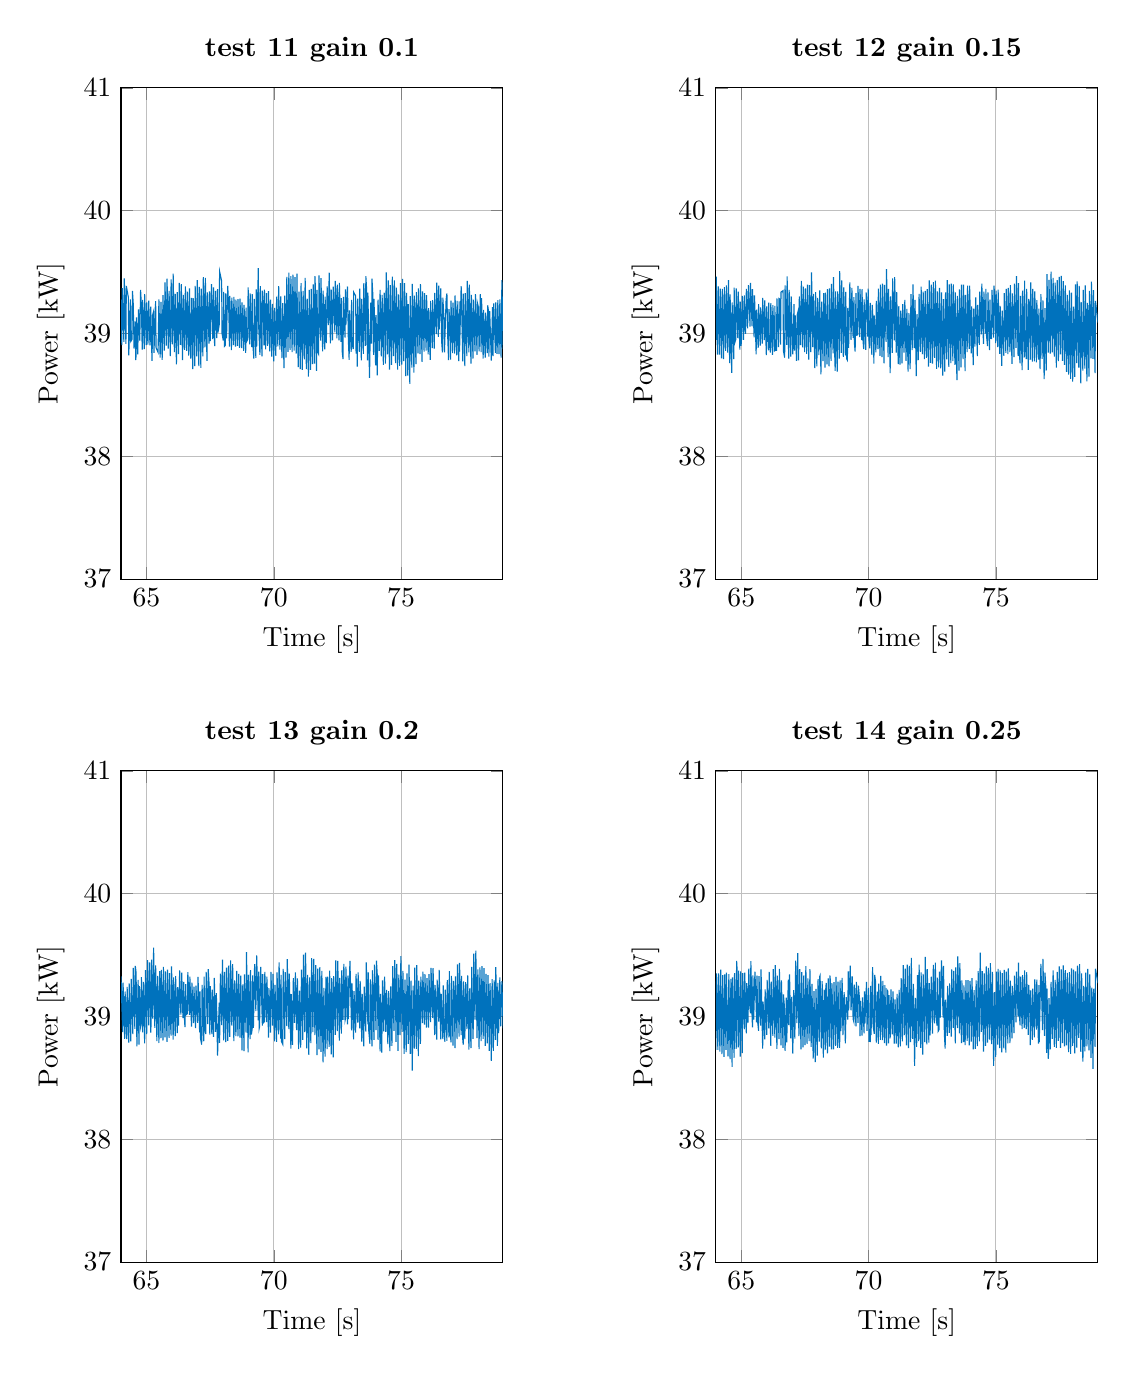
\begin{tikzpicture}

\begin{axis}[%
width=0.4\textwidth,
height=2.456in,
at={(1.026in,4.208in)},
scale only axis,
xmin=64,
xmax=79,
xlabel={Time [s]},
xmajorgrids,
ymin=37,
ymax=41,
ylabel={Power [kW]},
ymajorgrids,
axis background/.style={fill=white},
title style={font=\bfseries},
title={test 11 gain 0.1}
]
\addplot [color=mycolor1,solid,forget plot]
  table[row sep=crcr]{%
64	39.2762020802934\\
64.032	38.9057323467234\\
64.048	39.3682171040901\\
64.112	38.9324563121821\\
64.128	39.4485187027762\\
64.192	38.9156166032466\\
64.208	39.3873923021553\\
64.288	39.2937193125095\\
64.304	38.8207257210322\\
64.368	39.2772916774572\\
64.384	38.9348644550983\\
64.432	38.9525155278781\\
64.448	39.3470901387207\\
64.48	39.2436093192959\\
64.512	38.8769956603803\\
64.56	39.0973162928673\\
64.576	38.7839789269855\\
64.592	38.8186080828214\\
64.608	39.1304074910805\\
64.656	38.8289908104648\\
64.688	39.1952842906505\\
64.736	38.9410483431936\\
64.768	39.3539995737977\\
64.8	39.2277223523009\\
64.832	38.8685677434119\\
64.848	39.273874106812\\
64.912	38.8729468496124\\
64.928	39.3211534969397\\
64.992	38.9044346233041\\
65.008	39.2536809292504\\
65.056	38.9096269514025\\
65.088	39.2671029648071\\
65.136	38.9024022948011\\
65.168	39.2176809379522\\
65.216	38.7761406284406\\
65.248	39.1553467700377\\
65.28	39.1798165230385\\
65.296	38.8423035419562\\
65.312	38.9781470317512\\
65.36	39.262893765165\\
65.376	38.8837144296967\\
65.456	38.8465752106549\\
65.488	39.2776580139696\\
65.536	38.8041578980741\\
65.552	38.9753645071395\\
65.568	39.2578951141665\\
65.616	38.7843578957465\\
65.648	39.3112916335654\\
65.696	38.8598151823539\\
65.728	39.4150363934363\\
65.776	38.9005164447875\\
65.808	39.446639004233\\
65.856	38.8774144045713\\
65.888	39.3477298513702\\
65.92	38.9890475648346\\
65.936	38.8152464478799\\
65.968	39.4411258236354\\
66.016	38.9109563056839\\
66.048	39.4864975552604\\
66.096	38.8488341626943\\
66.128	39.3233139906334\\
66.176	38.7490104151546\\
66.208	39.3362690963806\\
66.256	38.8321710331453\\
66.288	39.4116706037236\\
66.336	38.9071511874216\\
66.368	39.40239448313\\
66.416	38.7822738761833\\
66.448	39.3143058661886\\
66.496	38.8664081642959\\
66.528	39.3828136260997\\
66.576	38.8585298477543\\
66.608	39.3414766909692\\
66.656	38.8200816502343\\
66.688	39.3668584890763\\
66.704	39.0116590772581\\
66.736	38.7944556905474\\
66.768	39.2890059119192\\
66.816	38.7088283126094\\
66.832	39.2881527444492\\
66.848	39.2556294553274\\
66.896	38.7341099656146\\
66.912	39.3874171029985\\
66.976	38.8128746475236\\
66.992	39.4343741016003\\
67.056	38.7346581756972\\
67.072	39.3796113904236\\
67.088	39.238637431133\\
67.136	38.7207041802726\\
67.152	39.3656429556886\\
67.216	38.8135220892151\\
67.232	39.4588632494492\\
67.296	38.8871128226859\\
67.312	39.4521062062171\\
67.376	38.7776252722741\\
67.392	39.3341982514618\\
67.456	38.918284754838\\
67.472	39.3430121760076\\
67.504	38.9373513033256\\
67.552	39.4012591789786\\
67.6	38.9532236605296\\
67.632	39.3750460997756\\
67.664	38.9591645772475\\
67.68	38.8971732092216\\
67.712	39.3458315991347\\
67.76	38.9627741479292\\
67.792	39.3606026465563\\
67.808	39.0080236738955\\
67.856	39.0700698560185\\
67.872	39.5054485614567\\
67.952	39.4264013256927\\
67.968	38.9989158565126\\
68.016	38.94302021923\\
68.032	39.3377036321191\\
68.064	38.8956896712969\\
68.096	38.9030488738434\\
68.112	39.325992542676\\
68.144	38.9600293371807\\
68.192	39.38830971318\\
68.24	39.1336677869143\\
68.256	38.892611589755\\
68.272	39.3051196725986\\
68.336	38.863764088747\\
68.352	39.2911679000998\\
68.416	38.9049117456133\\
68.432	39.2988203249823\\
68.496	38.8929439044956\\
68.512	39.2748481110375\\
68.576	38.8993529229338\\
68.592	39.2792054018347\\
68.656	38.882378703812\\
68.672	39.28316487493\\
68.736	38.8799508438361\\
68.752	39.2536963100034\\
68.816	38.8574105690252\\
68.832	39.2322749317016\\
68.896	38.8416001203239\\
68.912	39.2107057448974\\
68.928	38.931891906518\\
68.976	38.9523660379135\\
68.992	39.3745775739886\\
69.056	38.910411668419\\
69.072	39.3263140397299\\
69.136	38.8885940912699\\
69.152	39.3194351715121\\
69.168	38.9410597817387\\
69.216	38.7958730326358\\
69.232	39.2815931312213\\
69.296	38.800963501694\\
69.312	39.3583773773981\\
69.328	38.8929426652547\\
69.392	39.5323752412649\\
69.408	39.0503026904034\\
69.456	38.8264432068124\\
69.472	39.3863066002441\\
69.536	38.8131656416238\\
69.552	39.3480431009876\\
69.584	39.2382455295619\\
69.616	38.9023470820488\\
69.632	39.3564228090617\\
69.68	38.8698025270528\\
69.712	39.3292577557948\\
69.76	38.8982334911241\\
69.792	39.3454588571001\\
69.84	38.8547420711431\\
69.872	39.2760958940225\\
69.92	38.8105641109711\\
69.952	39.2417764695784\\
70	38.7731303404726\\
70.032	39.2084709900308\\
70.08	38.8173969646067\\
70.112	39.3001957329356\\
70.16	38.8954599161429\\
70.192	39.3858912317911\\
70.24	38.869496631731\\
70.272	39.3027939210474\\
70.32	38.7994697112423\\
70.336	38.9487541124288\\
70.352	39.246449784136\\
70.4	38.7179571619821\\
70.432	39.3086544526158\\
70.48	38.8043502631387\\
70.512	39.4608937727082\\
70.56	38.8500197212034\\
70.592	39.4954590541912\\
70.64	38.8673752413363\\
70.672	39.4678416911632\\
70.704	39.0654311712192\\
70.72	38.8472244182554\\
70.752	39.4792637280092\\
70.8	38.8609303356729\\
70.832	39.4577520908154\\
70.88	38.8349251994826\\
70.912	39.4869320671502\\
70.928	39.0722084077513\\
70.96	38.7251471801773\\
70.992	39.3404365720498\\
71.04	38.7101595369083\\
71.072	39.4089196402402\\
71.12	38.7029110108122\\
71.152	39.3465819407446\\
71.2	38.788274088865\\
71.232	39.4530358146862\\
71.28	38.7102236819299\\
71.312	39.2834490438861\\
71.36	38.6478276853189\\
71.392	39.3544779384791\\
71.44	38.7034785018255\\
71.472	39.3631987520711\\
71.488	39.0275260554134\\
71.52	38.7501692832027\\
71.552	39.3995750554482\\
71.6	38.7552630396261\\
71.616	39.4661140863577\\
71.632	39.3829076391922\\
71.68	38.6944807867308\\
71.696	39.355803725948\\
71.728	38.8480957852703\\
71.76	38.8327115533482\\
71.776	39.473188272486\\
71.84	38.9414398322586\\
71.856	39.451493138129\\
71.872	39.2448661014671\\
71.92	38.8536600944633\\
71.936	39.3490543548582\\
72	38.87028022877\\
72.016	39.2996678085141\\
72.064	38.9216031823876\\
72.096	39.3843734911536\\
72.144	39.0672860594381\\
72.176	39.4959614271415\\
72.224	38.918833703806\\
72.256	39.3562427316199\\
72.304	38.9444420416299\\
72.336	39.3815802804514\\
72.4	39.0083987043018\\
72.416	39.4287728630046\\
72.48	38.9607948607499\\
72.496	39.3973739974952\\
72.56	38.9442720664662\\
72.576	39.4119994525243\\
72.64	38.9311021968852\\
72.656	39.2878824422024\\
72.688	38.8513539998863\\
72.72	38.7912305803814\\
72.736	39.2976161185517\\
72.8	38.9668128590217\\
72.816	39.3581627470774\\
72.832	39.0687055967613\\
72.896	39.3823312781912\\
72.928	38.9554556695068\\
72.96	38.7854812820507\\
72.976	39.1885866547068\\
73.04	38.8499487124286\\
73.056	39.2729253590855\\
73.072	38.9260157411231\\
73.12	38.8726952388182\\
73.136	39.3372024757545\\
73.216	39.3050231632446\\
73.232	38.8365318662618\\
73.248	39.1596175261332\\
73.28	38.730505252806\\
73.296	39.2833980329105\\
73.36	38.8499318139231\\
73.376	39.3653710578892\\
73.44	38.7814688442226\\
73.456	39.2825630324714\\
73.52	38.8330426334993\\
73.536	39.4096168309749\\
73.6	38.8990265192246\\
73.616	39.4668559810247\\
73.648	39.3542242276422\\
73.68	38.7805465061242\\
73.696	39.3331261149724\\
73.76	38.6387594291315\\
73.808	39.2518948643169\\
73.84	38.9173967630013\\
73.856	39.4473103592857\\
73.888	39.3250828674127\\
73.92	38.8266799178914\\
73.936	39.2808560400678\\
74	38.7395216364588\\
74.016	39.1502989769223\\
74.064	38.6586611462352\\
74.096	39.2764916081819\\
74.144	38.8588361551561\\
74.176	39.3545988047872\\
74.224	38.8140530149036\\
74.256	39.3137649442224\\
74.304	38.7451765458287\\
74.336	39.3318061532072\\
74.368	39.1944939252269\\
74.384	38.754239795565\\
74.416	39.497837522224\\
74.464	38.8292277282082\\
74.496	39.4325024471798\\
74.544	38.7058603750506\\
74.576	39.3945373107367\\
74.624	38.7445681433715\\
74.64	39.0453122754243\\
74.656	39.4620175364551\\
74.704	38.8146188302235\\
74.736	39.4328034443926\\
74.784	38.7589010161484\\
74.816	39.3740739032756\\
74.864	38.7052265366874\\
74.896	39.3179008182708\\
74.944	38.7368590797633\\
74.976	39.4105738105486\\
75.024	38.7464949498182\\
75.056	39.4437362882567\\
75.104	38.7755955100252\\
75.136	39.40968929427\\
75.168	39.025977632577\\
75.184	38.6519447680024\\
75.216	39.3310144889428\\
75.264	38.6573664552143\\
75.28	39.2379760460158\\
75.344	38.5892188432456\\
75.36	39.3046157756235\\
75.392	38.9888973000357\\
75.424	38.7217995923211\\
75.44	39.4034829742204\\
75.504	38.6808887372103\\
75.52	39.3086153529126\\
75.536	39.202139239004\\
75.584	38.74955213243\\
75.6	39.3358313329971\\
75.664	38.8379021166863\\
75.68	39.3676479554169\\
75.744	38.8322831343736\\
75.76	39.4015157485903\\
75.824	38.7694409886483\\
75.84	39.3421140992453\\
75.904	38.8516460902513\\
75.92	39.328698747064\\
75.984	38.861171037037\\
76	39.3115480504011\\
76.064	38.829109571606\\
76.08	39.2069734495719\\
76.144	38.7845057647966\\
76.16	39.266192795428\\
76.224	38.8800239843935\\
76.24	39.2707150358355\\
76.304	38.8765788690564\\
76.32	39.3301869890028\\
76.384	38.9949484219248\\
76.4	39.4144175995293\\
76.464	38.9726638479843\\
76.48	39.3892795313954\\
76.496	39.0319413919716\\
76.56	39.3669219624178\\
76.592	38.9376809725204\\
76.624	38.8452711679987\\
76.64	39.2911048329326\\
76.688	39.1134177774774\\
76.704	38.846879827626\\
76.768	39.2742086184912\\
76.8	39.3261301702534\\
76.832	38.9720940618793\\
76.864	38.7837947508868\\
76.88	39.1973665533865\\
76.928	39.0695942453678\\
76.944	38.7871578887368\\
76.96	39.2681902508658\\
77.024	38.84024712865\\
77.04	39.2502635797122\\
77.104	38.8369608207161\\
77.12	39.3102711120494\\
77.184	38.821064011783\\
77.2	39.2649874943966\\
77.264	38.7741245971656\\
77.28	39.2619683195486\\
77.296	38.8527584051131\\
77.36	39.3860064118667\\
77.424	38.7733715456233\\
77.44	39.3239523032924\\
77.504	38.7345864016568\\
77.52	39.3292058770607\\
77.584	38.8153722142574\\
77.6	39.427868057664\\
77.664	38.8452340430412\\
77.68	39.3985832402384\\
77.744	38.7542218637409\\
77.76	39.3150920417966\\
77.824	38.7962054085567\\
77.84	39.2752686689125\\
77.888	38.9527525847283\\
77.904	38.8544635411059\\
77.92	39.3199868431531\\
77.984	38.8267489316809\\
78	39.2460448669003\\
78.032	39.2182517328484\\
78.064	38.8536335229105\\
78.112	39.3207686383144\\
78.144	38.8482082978926\\
78.16	39.288155070052\\
78.224	38.7962084370568\\
78.24	39.1924649623025\\
78.304	38.8025957985706\\
78.32	39.1703577615712\\
78.384	38.8405432751385\\
78.4	39.2292129889697\\
78.432	39.187163619141\\
78.448	38.8121532721648\\
78.48	39.1826772442034\\
78.544	38.7790660088408\\
78.592	39.2149680221404\\
78.608	38.8148460294721\\
78.64	39.2453685808663\\
78.704	38.8415806821339\\
78.72	39.2532928338798\\
78.768	38.8347676204539\\
78.784	38.951057078832\\
78.8	39.270857858118\\
78.848	38.8318687212617\\
78.88	39.2775070764734\\
78.928	38.8041225111169\\
78.96	39.4340447738484\\
79.008	38.8731214358441\\
};
\end{axis}

\begin{axis}[%
width=0.4\textwidth,
height=2.456in,
at={(4in,4.208in)},
scale only axis,
xmin=64,
xmax=79,
xlabel={Time [s]},
xmajorgrids,
ymin=37,
ymax=41,
ylabel={Power [kW]},
ymajorgrids,
axis background/.style={fill=white},
title style={font=\bfseries},
title={test 12  gain 0.15}
]
\addplot [color=mycolor1,solid,forget plot]
  table[row sep=crcr]{%
64	38.9485422143723\\
64.016	39.4620867407285\\
64.064	38.827704800368\\
64.096	39.383624248987\\
64.144	38.8268077806219\\
64.176	39.3656383881432\\
64.224	38.7965317427755\\
64.24	39.138919278395\\
64.256	39.3634677187056\\
64.304	38.7902603059519\\
64.336	39.3770713390022\\
64.384	38.8580828219533\\
64.416	39.3908919293428\\
64.464	38.8445102126791\\
64.496	39.4340416215506\\
64.544	38.7582676013644\\
64.56	39.3187251379994\\
64.624	38.6790357960774\\
64.64	39.2521038983653\\
64.704	38.791072930447\\
64.72	39.3736986001618\\
64.752	38.929499922466\\
64.784	38.9514841495229\\
64.8	39.3666750493033\\
64.864	38.9626477538581\\
64.88	39.3407685117419\\
64.944	38.8689954252475\\
64.96	39.258467600925\\
64.992	38.8990162992638\\
65.008	38.9547095324028\\
65.04	39.3064464448415\\
65.088	38.9479100039714\\
65.12	39.3101113716547\\
65.136	39.0497344310964\\
65.168	38.9973779779939\\
65.2	39.3637552609288\\
65.248	39.0416946137023\\
65.28	39.3940550413093\\
65.344	39.0555470917857\\
65.36	39.4127196617508\\
65.424	39.0584700848981\\
65.44	39.3601978917593\\
65.504	38.9688692806917\\
65.52	39.310895206825\\
65.584	38.8293258056645\\
65.6	39.1930996642073\\
65.664	38.8836974902241\\
65.68	39.2397885417096\\
65.744	38.900636989378\\
65.76	39.2127627881029\\
65.824	38.9168855801905\\
65.84	39.2902338046552\\
65.904	38.9459826183501\\
65.92	39.2703333410161\\
65.984	38.8232151647252\\
66	39.2203938615692\\
66.064	38.8617729634178\\
66.08	39.2505879412566\\
66.096	38.9232515433951\\
66.144	38.8448557308838\\
66.16	39.2473448268645\\
66.224	38.8257025912216\\
66.24	39.2301716077819\\
66.304	38.8516456840557\\
66.32	39.2239845386728\\
66.336	38.8636776329886\\
66.384	38.8629741037937\\
66.4	39.2851446132438\\
66.464	38.8893985050295\\
66.48	39.2845617729154\\
66.512	39.2800608005683\\
66.544	38.9092115604335\\
66.56	39.3368647552439\\
66.64	39.34853892606\\
66.656	38.8574477278905\\
66.704	38.8028107644704\\
66.72	39.3923428387449\\
66.784	38.9069594272576\\
66.8	39.4645272272431\\
66.864	38.7958408566649\\
66.88	39.3540806207595\\
66.944	38.8110689559281\\
66.96	39.3018632750116\\
67.024	38.8293627665507\\
67.072	39.2384959854459\\
67.088	38.8610581791265\\
67.12	39.1474582309694\\
67.168	38.7777812415512\\
67.2	39.154287584065\\
67.232	39.1806259094089\\
67.248	38.7802592975801\\
67.264	38.9824771902777\\
67.28	39.3009565367309\\
67.328	38.9060799578487\\
67.36	39.427767137212\\
67.408	38.8872286003149\\
67.44	39.3814794110381\\
67.488	38.8474864981558\\
67.52	39.3673670937423\\
67.568	38.8340907866731\\
67.6	39.398091927946\\
67.632	39.0753034968837\\
67.648	38.787223410324\\
67.68	39.3928569819749\\
67.728	38.8484379755839\\
67.76	39.4968225381609\\
67.808	38.8898289833658\\
67.84	39.321847145881\\
67.888	38.7175273011157\\
67.904	38.941404588168\\
67.92	39.3373083201308\\
67.968	38.7319599183849\\
68	39.290026988397\\
68.048	38.8231484154169\\
68.08	39.3498665360368\\
68.128	38.6673746303872\\
68.16	39.2590117592767\\
68.208	38.7741377847934\\
68.24	39.3286399476468\\
68.288	38.7214153585314\\
68.304	39.3315408397655\\
68.368	38.7485208842747\\
68.384	39.3611742587943\\
68.416	38.9640113710388\\
68.448	38.7326551168302\\
68.464	39.3663471014422\\
68.528	38.7772475400027\\
68.544	39.4028475488286\\
68.608	38.8377950228476\\
68.624	39.4588761267777\\
68.656	38.9343907179682\\
68.688	38.6952257813481\\
68.704	39.3422361284838\\
68.768	38.6899083569667\\
68.784	39.3420557649\\
68.8	39.2351720152118\\
68.848	38.7945934125847\\
68.864	39.5082832424154\\
68.928	38.8416940689345\\
68.944	39.4314123747707\\
69.008	38.8102304088538\\
69.024	39.3746840283916\\
69.088	38.8207845249844\\
69.104	39.3388186937766\\
69.136	38.7941418320562\\
69.168	38.7823395306708\\
69.184	39.2080395430294\\
69.216	38.8829433274696\\
69.264	39.4169665861977\\
69.312	38.9469567358863\\
69.344	39.3713659593714\\
69.392	38.9636931401566\\
69.424	39.2967787882112\\
69.44	38.9304600699564\\
69.472	38.8525183987384\\
69.504	39.3292247457569\\
69.52	38.9854596796576\\
69.568	38.9880676657597\\
69.584	39.3883324767739\\
69.648	38.9710501725036\\
69.664	39.3624394160763\\
69.728	38.9455755012801\\
69.744	39.3618239444401\\
69.776	38.9586418287371\\
69.808	38.8727883913063\\
69.824	39.2775063116274\\
69.888	38.866118637856\\
69.904	39.3337044286414\\
69.952	39.1980937028364\\
69.968	38.9743353123122\\
69.984	39.3642505634073\\
70.016	38.9433700222145\\
70.048	38.8787647171583\\
70.064	39.2484817082717\\
70.128	38.8266037386974\\
70.144	39.232842618648\\
70.192	39.035070974928\\
70.208	38.7552758273133\\
70.224	39.14619074476\\
70.288	38.845959942249\\
70.304	39.2645706264278\\
70.368	38.8724483486127\\
70.384	39.3643751586212\\
70.448	38.8185829898815\\
70.464	39.3978277026991\\
70.528	38.8082410484231\\
70.544	39.4064309252231\\
70.608	38.7567444073467\\
70.624	39.3952562211977\\
70.688	38.9310526464287\\
70.704	39.5243016799893\\
70.768	38.8077748814051\\
70.784	39.3628128065948\\
70.848	38.6780382769399\\
70.864	39.3016751403577\\
70.928	38.8411560962232\\
70.944	39.4483469886712\\
71.008	38.9431132203559\\
71.024	39.4595839326866\\
71.088	38.8445595366977\\
71.104	39.335961927316\\
71.152	38.8573177778184\\
71.168	38.7498886645005\\
71.184	39.2215778358377\\
71.232	38.7464388382118\\
71.264	39.1851927846571\\
71.296	39.0761934170224\\
71.312	38.75718798485\\
71.344	39.2387221537134\\
71.392	38.843320198458\\
71.424	39.2740788286307\\
71.472	38.775983660695\\
71.504	39.2004048327527\\
71.552	38.6890042409222\\
71.584	39.1663571459991\\
71.632	38.7103501161956\\
71.664	39.3206267879482\\
71.712	38.8650839661932\\
71.744	39.4002044306757\\
71.792	38.8817072979006\\
71.824	39.2726340084584\\
71.872	38.6528072465055\\
71.904	39.1565093758033\\
71.952	38.7826466991267\\
71.984	39.3219835497165\\
72.032	38.8506923361483\\
72.048	39.051536831757\\
72.064	39.3813959594512\\
72.112	38.8308358961756\\
72.144	39.3412876746828\\
72.192	38.7902283266997\\
72.224	39.3468817024838\\
72.272	38.8022483029367\\
72.288	38.9205685628886\\
72.304	39.36021429265\\
72.352	38.7304333462679\\
72.384	39.4324409693532\\
72.432	38.7597711917734\\
72.464	39.3985697433592\\
72.512	38.7547067704723\\
72.544	39.4173863039318\\
72.592	38.8009195215514\\
72.624	39.4300844024336\\
72.672	38.7111676416913\\
72.688	39.0198388615532\\
72.704	39.3429774246662\\
72.752	38.7240846305712\\
72.784	39.3710693824951\\
72.832	38.7167230312114\\
72.864	39.334911909626\\
72.912	38.6575273967105\\
72.944	39.2793879934181\\
72.992	38.6902954497868\\
73.024	39.3343427136509\\
73.072	38.7885259079529\\
73.088	39.4342391647485\\
73.152	38.7274044547127\\
73.168	39.4003465900889\\
73.232	38.7576973844733\\
73.248	39.4051069750993\\
73.312	38.7751241135521\\
73.328	39.4000734684101\\
73.392	38.7441036350111\\
73.408	39.3345855569316\\
73.44	38.8664877480091\\
73.472	38.6194456014692\\
73.488	39.3052668814107\\
73.552	38.6983477083738\\
73.568	39.3593818919904\\
73.584	39.2569635870417\\
73.632	38.7246142402725\\
73.648	39.3973510073978\\
73.712	38.7902662924978\\
73.728	39.3971832498382\\
73.792	38.6932101057283\\
73.808	39.3137320453866\\
73.824	39.1624090377997\\
73.872	38.8473073946639\\
73.888	39.3886666179833\\
73.952	38.8751773851277\\
73.968	39.3885685614453\\
74.032	38.8381655702196\\
74.048	39.2206854143751\\
74.112	38.7427574639355\\
74.128	39.2016144878847\\
74.176	38.892069692379\\
74.208	39.2936737537542\\
74.272	38.8164522449742\\
74.288	39.2321807290359\\
74.352	38.907429828397\\
74.368	39.3410610158335\\
74.432	38.9922604977687\\
74.448	39.4059223319646\\
74.512	38.9159190945974\\
74.528	39.3410279646406\\
74.592	38.9998411539122\\
74.608	39.3623774671718\\
74.624	38.9990845398255\\
74.672	38.8975508790195\\
74.688	39.3352829412277\\
74.752	38.8649422716422\\
74.768	39.2757417490372\\
74.784	38.9613416639156\\
74.832	38.9588434482234\\
74.848	39.3557253346074\\
74.912	38.9656311750012\\
74.928	39.3893731664959\\
74.976	39.1658998444518\\
74.992	38.921594191799\\
75.008	39.3489574663961\\
75.072	38.8892575098213\\
75.088	39.3561063298224\\
75.152	38.8336672750793\\
75.168	39.2253897222516\\
75.232	38.7363189630487\\
75.248	39.1866337069428\\
75.312	38.8182444012636\\
75.328	39.3281727420458\\
75.392	38.8415944465224\\
75.408	39.3630934412665\\
75.472	38.8320306201375\\
75.488	39.3716429577508\\
75.552	38.8483754754218\\
75.568	39.3938876480146\\
75.632	38.7525022460525\\
75.648	39.3260633226033\\
75.712	38.8067602489983\\
75.728	39.4061171158882\\
75.792	38.8830640709146\\
75.808	39.4676023808825\\
75.872	38.8183144304261\\
75.888	39.4100657458799\\
75.904	38.8762427175436\\
75.952	38.7571365614949\\
75.968	39.3060595501223\\
76.032	38.7009835440467\\
76.048	39.3489298834112\\
76.112	38.8035008905314\\
76.128	39.4310988784543\\
76.144	38.9547035189546\\
76.192	38.7904366012678\\
76.208	39.3621854919726\\
76.272	38.7042839872046\\
76.288	39.2809150448523\\
76.32	39.2460017895486\\
76.352	38.7860257766483\\
76.368	39.4161358254941\\
76.432	38.7706962031122\\
76.448	39.3621078268532\\
76.512	38.7726497258406\\
76.528	39.3420977521133\\
76.592	38.7642105880715\\
76.608	39.2707203393715\\
76.672	38.7861786718486\\
76.688	39.2025257069423\\
76.736	38.7090833193067\\
76.768	39.3209934430722\\
76.816	38.7937922883756\\
76.848	39.2686287034675\\
76.896	38.6290714322358\\
76.928	39.2067304737317\\
76.976	38.6965896152524\\
77.008	39.483596445264\\
77.056	38.8440565333994\\
77.072	38.9996856534572\\
77.088	39.4364580015034\\
77.136	38.8358285344588\\
77.168	39.5029300868737\\
77.216	38.8453182930918\\
77.248	39.4524562614407\\
77.296	38.8109291555893\\
77.328	39.4145900683667\\
77.376	38.7212351321712\\
77.408	39.4352837268891\\
77.44	39.1149618814258\\
77.456	38.7752664789708\\
77.488	39.4600711882369\\
77.536	38.8301117955662\\
77.568	39.4689667868723\\
77.616	38.7770738348243\\
77.648	39.4265394554044\\
77.696	38.7438581099545\\
77.712	38.9985048534317\\
77.728	39.3913017095156\\
77.776	38.6864016909411\\
77.808	39.31498663255\\
77.856	38.6641390035486\\
77.888	39.3516479245764\\
77.936	38.6301310715794\\
77.968	39.33253962841\\
78.016	38.6071276225846\\
78.048	39.2185783435048\\
78.096	38.646998712819\\
78.128	39.3997303504282\\
78.176	38.7582445327251\\
78.192	39.4244923130413\\
78.224	39.0739524769288\\
78.256	38.7220316846683\\
78.272	39.3869674667396\\
78.336	38.5942097521262\\
78.352	39.2541267543102\\
78.416	38.6965396352241\\
78.432	39.3541360797471\\
78.464	38.9610065263489\\
78.496	38.7142863719012\\
78.512	39.3916392226942\\
78.576	38.6108407545775\\
78.592	39.248394319827\\
78.608	39.18189363847\\
78.656	38.6477699428183\\
78.672	39.3461083968433\\
78.736	38.7963052256403\\
78.752	39.4218257660927\\
78.816	38.7930243585108\\
78.832	39.3520213798369\\
78.896	38.678001411236\\
78.912	39.2648170949767\\
79.008	39.0868592335425\\
};
\end{axis}

\begin{axis}[%
width=0.4\textwidth,
height=2.456in,
at={(1.026in,0.793in)},
scale only axis,
xmin=64,
xmax=79,
xlabel={Time [s]},
xmajorgrids,
ymin=37,
ymax=41,
ylabel={Power [kW]},
ymajorgrids,
axis background/.style={fill=white},
title style={font=\bfseries},
title={test 13  gain 0.2}
]
\addplot [color=mycolor1,solid,forget plot]
  table[row sep=crcr]{%
64	39.3272219695461\\
64.064	38.8726640819004\\
64.08	39.2750679396056\\
64.144	38.8173325716961\\
64.16	39.2031948844495\\
64.224	38.8147982113799\\
64.24	39.2412552818442\\
64.304	38.787125542179\\
64.32	39.269533476915\\
64.384	38.7964062952539\\
64.4	39.3060727922415\\
64.464	38.8563610577548\\
64.48	39.3962842306039\\
64.544	38.8993046871526\\
64.56	39.4118074424533\\
64.592	39.3579696037556\\
64.624	38.7555514923622\\
64.672	39.2974767960638\\
64.704	38.7705187818815\\
64.72	39.2467642806199\\
64.768	38.9188930750078\\
64.784	38.9378245882146\\
64.8	39.3212863987839\\
64.848	38.8702449961728\\
64.88	39.2811895551924\\
64.928	38.7810215276896\\
64.96	39.3775554615073\\
65.008	38.8555971314907\\
65.04	39.4593648560398\\
65.088	38.9268318255197\\
65.12	39.4396296387522\\
65.152	39.1278330975121\\
65.168	38.8676477370571\\
65.184	38.9651406195481\\
65.2	39.4631017005791\\
65.248	38.9830600201153\\
65.28	39.5607676620856\\
65.328	38.9078365219893\\
65.36	39.4161273022073\\
65.408	38.7999977187025\\
65.44	39.3302180147335\\
65.488	38.7840102539595\\
65.52	39.3692433090441\\
65.568	38.8230206751624\\
65.584	39.379038956026\\
65.648	38.8043799768843\\
65.664	39.4044559411042\\
65.728	38.8306901943667\\
65.744	39.3663646552617\\
65.808	38.7941019855461\\
65.824	39.3822383834459\\
65.888	38.8250029509385\\
65.904	39.3537896455369\\
65.936	38.9657703265806\\
65.968	38.8447946593574\\
65.984	39.4080911351237\\
66.048	38.8109951918688\\
66.064	39.3183814449071\\
66.08	39.2013211710519\\
66.128	38.8407053301368\\
66.144	39.3294547042279\\
66.208	38.864571702836\\
66.224	39.2385624139697\\
66.256	38.9251564643593\\
66.304	39.3745842511384\\
66.32	39.144102684634\\
66.352	39.0150437586282\\
66.384	39.356279753114\\
66.432	38.9869913695356\\
66.464	39.2809355574797\\
66.496	38.961435383005\\
66.512	38.9141981897925\\
66.544	39.2627476056587\\
66.56	39.0146209559097\\
66.608	39.02331667723\\
66.624	39.3605762804471\\
66.688	39.0122921711614\\
66.704	39.3252331124908\\
66.768	38.9179730133677\\
66.784	39.2759465261655\\
66.848	38.9466929978769\\
66.864	39.2424323410987\\
66.928	38.9059600878807\\
66.944	39.2513557435497\\
67.008	38.9488696294203\\
67.024	39.3214712402048\\
67.088	38.870893174451\\
67.104	39.2048661489311\\
67.12	38.8237573929191\\
67.168	38.7703640726192\\
67.184	39.2564698579387\\
67.248	38.7983058367442\\
67.264	39.3251163136086\\
67.28	38.9155180924193\\
67.328	38.8568887177973\\
67.344	39.3636602503259\\
67.408	38.9384894719901\\
67.424	39.3856867464113\\
67.456	39.2742709930977\\
67.488	38.8526567419788\\
67.504	39.2475815035169\\
67.568	38.85636481922\\
67.584	39.217553552112\\
67.632	38.8341739825618\\
67.664	39.3147007887613\\
67.712	38.8736490402292\\
67.744	39.1897870311159\\
67.792	38.6820447410117\\
67.856	39.1126931316068\\
67.872	38.7842299402897\\
67.904	39.3493575175907\\
67.952	38.9305530639112\\
67.984	39.4633703515996\\
68.032	38.8053018588909\\
68.064	39.364045100489\\
68.112	38.7902062160342\\
68.144	39.3975019770051\\
68.192	38.801860968709\\
68.208	38.9431512833636\\
68.224	39.4137588463568\\
68.272	38.8343519672957\\
68.304	39.456107586643\\
68.352	38.9245424539473\\
68.384	39.4253416831856\\
68.432	38.7989398485418\\
68.464	39.2932403018581\\
68.512	38.8407309154986\\
68.544	39.3703710872569\\
68.592	38.8371895176907\\
68.624	39.3472589759908\\
68.672	38.8275103702504\\
68.704	39.3325288485638\\
68.752	38.7234550711235\\
68.784	39.2615849728685\\
68.832	38.717657346643\\
68.848	39.3422638639631\\
68.912	38.868652910062\\
68.928	39.5245501227056\\
68.992	38.7080992080118\\
69.008	39.3396493458581\\
69.072	38.8163766353316\\
69.088	39.377280562461\\
69.12	38.8520135983645\\
69.152	38.8983862603014\\
69.168	39.3340903317349\\
69.2	38.9072378346175\\
69.248	39.4255418523196\\
69.296	39.0445981203994\\
69.328	39.4969821163273\\
69.392	38.9672770023109\\
69.408	39.3644493757436\\
69.424	38.9001928821712\\
69.44	38.915555121902\\
69.488	39.4035094979234\\
69.552	38.9253598814929\\
69.568	39.3445059322431\\
69.6	38.9504533113488\\
69.632	38.9579057658999\\
69.648	39.3626745871447\\
69.712	38.9541840749817\\
69.728	39.3243801585366\\
69.776	39.0178383214692\\
69.792	38.8285411221373\\
69.808	39.2302358321593\\
69.872	38.8690171968957\\
69.888	39.3637035859908\\
69.952	38.9248334326704\\
69.968	39.3457931644051\\
70.032	38.7974790678372\\
70.048	39.2563783532946\\
70.112	38.7932582531295\\
70.128	39.3584895986989\\
70.192	38.8547194073213\\
70.208	39.4408079516345\\
70.272	38.8194843704775\\
70.288	39.3381729486916\\
70.304	38.7944382125879\\
70.352	38.7738847196286\\
70.368	39.3877982735319\\
70.432	38.8160089120267\\
70.448	39.3618622138237\\
70.512	38.9223362739095\\
70.528	39.4670902982946\\
70.592	38.8964241416681\\
70.608	39.3478498690644\\
70.672	38.7383242387392\\
70.688	39.1828536838993\\
70.736	38.7687343875566\\
70.768	39.3128687057756\\
70.816	38.9470244716389\\
70.848	39.3597025741307\\
70.896	38.8890372003397\\
70.928	39.3099886575313\\
70.976	38.7346907361725\\
71.008	39.209485495804\\
71.056	38.7468575701616\\
71.088	39.3820287931669\\
71.12	39.1098833028226\\
71.136	38.8092101370213\\
71.168	39.5036437568583\\
71.216	38.8731523211212\\
71.248	39.5205312223126\\
71.296	38.7396855182087\\
71.328	39.3385790780225\\
71.376	38.6878062169996\\
71.408	39.3177998918771\\
71.456	38.7824843656324\\
71.488	39.4750678313997\\
71.536	38.8725847306131\\
71.568	39.4685828171123\\
71.616	38.847902995208\\
71.648	39.4182466172504\\
71.696	38.6846288573046\\
71.728	39.3899232464325\\
71.776	38.7314387881351\\
71.808	39.4022470307614\\
71.856	38.7109717418995\\
71.888	39.3709888203872\\
71.92	38.8743624157082\\
71.936	38.6253619231373\\
71.968	39.2324472768493\\
72.016	38.6723066764291\\
72.048	39.3215495762297\\
72.096	38.7347708888484\\
72.112	39.3246335979373\\
72.176	38.7518595882286\\
72.192	39.373914924442\\
72.256	38.6911620358071\\
72.272	39.3111594433839\\
72.288	39.2745757540609\\
72.336	38.6664927447184\\
72.352	39.3284909245538\\
72.416	38.8503998194141\\
72.432	39.457557140086\\
72.496	38.8804979061634\\
72.512	39.4534125940867\\
72.576	38.8027393949993\\
72.592	39.3146181816105\\
72.656	38.8601692926189\\
72.672	39.3780638462349\\
72.72	38.9720712048292\\
72.752	39.4290281518668\\
72.8	38.9671952980137\\
72.816	38.982020058501\\
72.832	39.4056016531548\\
72.896	38.9360943183913\\
72.912	39.3317937036874\\
72.928	38.9781849109132\\
72.992	39.4528439705887\\
73.056	38.8873695317459\\
73.072	39.2684300719643\\
73.136	38.8126922068777\\
73.152	39.2070954290053\\
73.216	38.8691805468473\\
73.232	39.3468094684195\\
73.264	39.1040225955572\\
73.296	38.9497128256671\\
73.312	39.3597236965362\\
73.376	38.9039080001592\\
73.392	39.290692590818\\
73.424	39.0906329228489\\
73.456	38.7945673353683\\
73.472	39.1845795595567\\
73.536	38.7567965516852\\
73.552	39.2431252544949\\
73.616	38.8758373344771\\
73.632	39.440133399071\\
73.696	38.9356579830056\\
73.712	39.3584669431722\\
73.728	38.8894583344484\\
73.776	38.7772238230719\\
73.792	39.3022404508963\\
73.856	38.7559480690832\\
73.872	39.3762943242871\\
73.936	38.8092809332365\\
73.952	39.4225359830966\\
74.016	38.8896305617732\\
74.032	39.4554042401668\\
74.064	39.3412946563747\\
74.096	38.8096002199791\\
74.112	39.3351223681093\\
74.176	38.7154681138836\\
74.192	39.1835872885546\\
74.24	38.7065156010019\\
74.272	39.2931088172761\\
74.32	38.8786663352487\\
74.352	39.3250544916674\\
74.4	38.8746322823748\\
74.432	39.2174298594279\\
74.48	38.774045903667\\
74.512	39.2056054450022\\
74.56	38.7171695248866\\
74.592	39.2449444775074\\
74.64	38.7596147590533\\
74.672	39.4098363585838\\
74.72	38.8822437671651\\
74.752	39.4584844728713\\
74.784	39.1741369039661\\
74.8	38.7935351892143\\
74.832	39.4272774398852\\
74.88	38.7208650564723\\
74.912	39.3397340612934\\
74.96	38.8487471714383\\
74.992	39.4914255927282\\
75.04	38.8738444285982\\
75.072	39.3714868188808\\
75.12	38.6944638426779\\
75.152	39.3008958405586\\
75.2	38.7088170880527\\
75.232	39.3500007454668\\
75.28	38.7769452465611\\
75.312	39.4215566882398\\
75.36	38.6945903120346\\
75.392	39.2919332296195\\
75.44	38.5591118532671\\
75.472	39.2511194722687\\
75.52	38.7391314779341\\
75.536	39.3970305465038\\
75.568	39.0136989941766\\
75.6	38.7358142917887\\
75.616	39.4173060789711\\
75.68	38.6772326890654\\
75.696	39.2912918681778\\
75.712	39.1692363591756\\
75.76	38.7767087056478\\
75.776	39.324910262919\\
75.84	38.9450684031533\\
75.856	39.3650112593197\\
75.92	38.9329602847692\\
75.936	39.3454264825423\\
76	38.9094364781222\\
76.016	39.3129893268913\\
76.08	38.9090403419665\\
76.096	39.3454220579332\\
76.16	38.9532317573694\\
76.176	39.396300864078\\
76.24	38.9885014689786\\
76.256	39.3942491250535\\
76.32	38.8474100458047\\
76.336	39.2546939423644\\
76.4	38.8111534499628\\
76.416	39.3004181623438\\
76.48	38.958657474922\\
76.496	39.3799318447346\\
76.56	38.8135417334716\\
76.576	39.1845262300443\\
76.64	38.8159707248364\\
76.656	39.2535287190868\\
76.672	38.9482018080121\\
76.72	38.7938539604072\\
76.736	39.2175255431169\\
76.8	38.8004361892772\\
76.816	39.295756969608\\
76.88	38.8295331176402\\
76.896	39.3701438306429\\
76.912	38.9407169034014\\
76.96	38.7895587836955\\
76.976	39.3306191432707\\
77.04	38.7628704001115\\
77.056	39.2888028907202\\
77.088	39.1728707240685\\
77.12	38.7422718729708\\
77.136	39.3264651240733\\
77.2	38.8146451291785\\
77.216	39.424339979998\\
77.28	38.8368583138642\\
77.296	39.4360568638779\\
77.36	38.8477266058403\\
77.376	39.3301879952789\\
77.424	38.81096649191\\
77.44	38.7705637138181\\
77.456	39.2863092140563\\
77.504	38.8153121760466\\
77.536	39.2796610043544\\
77.584	38.8978423798855\\
77.616	39.3354282787649\\
77.664	38.729056273161\\
77.696	39.2291632688726\\
77.744	38.7417910974222\\
77.776	39.4041423080224\\
77.824	38.817968947732\\
77.84	38.9643252221796\\
77.856	39.5117848987935\\
77.904	38.9752529039367\\
77.936	39.5361023112225\\
77.984	38.8229198545134\\
78.016	39.3827588387719\\
78.064	38.7333914190064\\
78.096	39.4004314777719\\
78.144	38.7999709603711\\
78.176	39.4100146857922\\
78.224	38.8184247683385\\
78.24	39.1506797100299\\
78.256	39.3927713678653\\
78.304	38.760837396273\\
78.336	39.3468074392395\\
78.384	38.7816445902693\\
78.416	39.3356314631339\\
78.464	38.7196894559863\\
78.48	39.1778375043675\\
78.496	39.2706992999708\\
78.544	38.6387466845065\\
78.576	39.30397407575\\
78.624	38.7205468172308\\
78.656	39.2939074889631\\
78.704	38.8087786837324\\
78.72	39.4012726901805\\
78.784	38.7599588561701\\
78.8	39.2725091412098\\
78.832	38.8653171276125\\
78.88	39.3192419876937\\
78.912	38.9188789976792\\
78.96	39.2883365817962\\
79.008	38.9028328410321\\
};
\end{axis}

\begin{axis}[%
width=0.4\textwidth,
height=2.456in,
at={(4in,0.793in)},
scale only axis,
xmin=64,
xmax=79,
xlabel={Time [s]},
xmajorgrids,
ymin=37,
ymax=41,
ylabel={Power [kW]},
ymajorgrids,
axis background/.style={fill=white},
title style={font=\bfseries},
title={test 14  gain 0.25}
]
\addplot [color=mycolor1,solid,forget plot]
  table[row sep=crcr]{%
64	38.7281169727752\\
64.032	39.3504352163319\\
64.08	38.7275336593424\\
64.112	39.3510828857088\\
64.16	38.714674594242\\
64.192	39.3822401661287\\
64.24	38.6937830888749\\
64.272	39.337441015494\\
64.32	38.6706638043943\\
64.352	39.3421445151568\\
64.4	38.7282945883297\\
64.416	39.357904030536\\
64.48	38.6756797131583\\
64.512	39.3449360175572\\
64.56	38.6524180971823\\
64.592	39.3068634012588\\
64.64	38.5894677859406\\
64.656	39.3174175530407\\
64.72	38.6638760948758\\
64.736	39.352380788371\\
64.8	38.7361666882483\\
64.816	39.4533041531508\\
64.832	39.3974372039193\\
64.88	38.7480432583812\\
64.896	39.3738848442953\\
64.96	38.6733283562772\\
64.976	39.366685152574\\
65.04	38.7010159020342\\
65.056	39.3531660083099\\
65.12	38.8959830697133\\
65.136	39.3562492305525\\
65.184	38.9231612063516\\
65.2	38.8627790834774\\
65.216	39.2719553020354\\
65.264	38.9499502818357\\
65.296	39.3889372919652\\
65.328	39.099885977748\\
65.36	39.0254882675831\\
65.376	39.4498612879288\\
65.424	38.9997663079607\\
65.44	38.9120326284458\\
65.456	39.3341952162449\\
65.488	38.9745547474427\\
65.536	39.3648001387548\\
65.584	39.0905105774434\\
65.6	38.9509998778632\\
65.616	39.3327558491616\\
65.648	38.9457910437407\\
65.68	38.8833826073659\\
65.696	39.3291218510277\\
65.76	38.9260682135083\\
65.776	39.3825229904985\\
65.84	38.7386604774763\\
65.856	39.1216841247173\\
65.92	38.813703886404\\
65.936	39.2214485049353\\
66	38.8498452383196\\
66.016	39.2977915677844\\
66.08	38.9028258034389\\
66.096	39.3626925658283\\
66.16	38.760107140783\\
66.176	39.2826599001582\\
66.24	38.8423598705556\\
66.256	39.3859235787269\\
66.32	38.8286051349029\\
66.336	39.4187058614676\\
66.4	38.7366329472076\\
66.416	39.3332024319258\\
66.48	38.8152114868081\\
66.496	39.3874996309299\\
66.544	38.9770493564968\\
66.56	38.7645346330179\\
66.576	39.2939624834974\\
66.64	38.7451474606575\\
66.656	39.1791784382631\\
66.688	39.0975444628961\\
66.72	38.720631935215\\
66.768	39.1531385996402\\
66.784	38.7884737908115\\
66.848	39.2993443386843\\
66.864	38.9294237666987\\
66.896	39.3420339917518\\
66.944	38.8210637684083\\
66.976	39.1594703421472\\
67.024	38.6974102939477\\
67.056	39.2145553352007\\
67.104	38.8188647246012\\
67.136	39.4536886840411\\
67.184	38.9466620665385\\
67.216	39.5158220930212\\
67.264	38.8394769452394\\
67.296	39.3850167350283\\
67.344	38.7311564403126\\
67.376	39.3604720857573\\
67.424	38.7478105993629\\
67.456	39.3350793788279\\
67.472	39.0016825260537\\
67.504	38.7670497166908\\
67.536	39.4101203753032\\
67.584	38.7771709587162\\
67.616	39.3099425447439\\
67.664	38.7991243478888\\
67.696	39.3855453483695\\
67.744	38.7518707864266\\
67.776	39.2656821232783\\
67.824	38.6568141512792\\
67.856	39.2057332292559\\
67.904	38.6273553734061\\
67.936	39.2241766736051\\
67.984	38.6807790799221\\
68.016	39.3040306664473\\
68.064	38.7948379058702\\
68.08	39.3248124307477\\
68.096	39.3335899507559\\
68.144	38.7400654434939\\
68.176	39.2886753604836\\
68.224	38.6655068613621\\
68.256	39.2190062623607\\
68.304	38.7307409606425\\
68.32	39.2361608311704\\
68.336	39.2723962443838\\
68.384	38.6988183183068\\
68.416	39.3105029176405\\
68.464	38.7547573408886\\
68.48	39.3345858371069\\
68.496	39.2989620182563\\
68.544	38.7311046832216\\
68.56	39.2707143856433\\
68.624	38.7324563777156\\
68.64	39.2789454511937\\
68.704	38.7597684823461\\
68.72	39.3227529146156\\
68.784	38.7440940142967\\
68.8	39.2834732436525\\
68.832	38.8424042815404\\
68.864	38.7436794935058\\
68.88	39.2947115738747\\
68.912	38.881337076387\\
68.96	39.3142416054337\\
68.976	39.1234952410273\\
68.992	38.848158983833\\
69.04	39.1983184587877\\
69.088	38.7813048395945\\
69.12	39.1572390755713\\
69.184	38.9745296089657\\
69.2	39.366782348108\\
69.216	39.0494191207538\\
69.28	39.4133904614544\\
69.312	39.0492986792814\\
69.36	39.3260334207566\\
69.392	38.9798049486486\\
69.424	38.9551687464623\\
69.44	39.2587847231052\\
69.504	38.919528829915\\
69.52	39.2820531498241\\
69.584	38.9476229787863\\
69.6	39.2509841390603\\
69.648	39.1340633406002\\
69.664	38.8404610993751\\
69.68	39.1272502141869\\
69.744	38.8450099537657\\
69.76	39.1548701856592\\
69.824	38.8632197741514\\
69.84	39.2035348161062\\
69.856	38.9427778914319\\
69.92	39.2822515599155\\
69.936	38.8831309977723\\
70	39.2337021109099\\
70.016	38.7973057856107\\
70.064	38.7963014698804\\
70.08	39.2481405013548\\
70.096	38.8477861386135\\
70.16	39.4026382624138\\
70.176	38.9260288852803\\
70.224	38.859132955103\\
70.24	39.33907378938\\
70.272	39.2868821776796\\
70.304	38.788033411927\\
70.352	39.2027568842283\\
70.384	38.7772378867221\\
70.4	39.2664943529423\\
70.464	38.8087491969856\\
70.48	39.3310750031721\\
70.544	38.8079771594181\\
70.56	39.2891713112158\\
70.624	38.7822158771175\\
70.64	39.254994450249\\
70.704	38.7626731445454\\
70.72	39.2174446153355\\
70.752	39.206874789281\\
70.784	38.7817788662504\\
70.8	39.1730388912514\\
70.848	38.8215332805745\\
70.88	39.2200770914\\
70.928	38.8539585146187\\
70.96	39.2047724331552\\
71.008	38.778031361165\\
71.04	39.1391147342433\\
71.088	38.7798545950133\\
71.104	38.9242208918746\\
71.12	39.1829009768902\\
71.168	38.7477703373153\\
71.2	39.2167896487372\\
71.248	38.755801821808\\
71.28	39.3123198565499\\
71.328	38.7981943379188\\
71.36	39.4179690587033\\
71.408	38.8490337200132\\
71.44	39.3886398048566\\
71.456	39.0863248242072\\
71.488	38.7649017818956\\
71.52	39.4224666905088\\
71.568	38.7431203134118\\
71.6	39.4114952977504\\
71.648	38.7904299263309\\
71.68	39.4762353436864\\
71.696	39.1114426554264\\
71.728	38.8172027550887\\
71.76	39.2643937332995\\
71.808	38.5981327177262\\
71.84	39.1511013511194\\
71.888	38.7523315382882\\
71.92	39.3372771186164\\
71.968	38.7984528733108\\
71.984	39.4225835241032\\
72.048	38.7433122993678\\
72.064	39.3583622142612\\
72.128	38.6897595657262\\
72.144	39.347171960053\\
72.208	38.7917589496737\\
72.224	39.4860093606407\\
72.288	38.7720522862543\\
72.304	39.3847454420739\\
72.368	38.7868319555181\\
72.384	39.2717873576886\\
72.416	38.8451755354284\\
72.464	39.3247155154478\\
72.512	38.8602584254742\\
72.544	39.4203593609482\\
72.592	38.9439670557327\\
72.624	39.4384643346915\\
72.64	39.0333801951106\\
72.688	38.9258648608905\\
72.704	39.3153164011964\\
72.736	38.8812944341844\\
72.768	38.894214945526\\
72.784	39.365393701485\\
72.816	38.9908412295019\\
72.864	39.4566585825231\\
72.928	38.990439624666\\
72.944	39.4115946183465\\
72.976	38.8598630714862\\
73.008	38.7379421420197\\
73.024	39.136900695084\\
73.088	38.8426967600209\\
73.104	39.2497187525008\\
73.168	38.866825098105\\
73.184	39.2695272473395\\
73.248	38.8356900724351\\
73.264	39.384173096434\\
73.328	38.9067532875944\\
73.344	39.3717696573021\\
73.408	38.7808442926166\\
73.424	39.4001785402081\\
73.488	38.9050178947299\\
73.504	39.4898249861164\\
73.568	38.8615840176178\\
73.584	39.4345023834226\\
73.632	38.9487847850146\\
73.648	38.7839009647809\\
73.664	39.2942357901891\\
73.728	38.7909454782309\\
73.744	39.2533121245111\\
73.792	38.7657376237979\\
73.824	39.2968616472079\\
73.872	38.8013029243414\\
73.904	39.2960009559877\\
73.952	38.7644553779886\\
73.984	39.2889943524366\\
74.016	39.156179526464\\
74.032	38.7942675738482\\
74.064	39.3117180661151\\
74.112	38.7327291702082\\
74.144	39.2153224006844\\
74.192	38.7365192007436\\
74.224	39.2946143771252\\
74.272	38.7585496509074\\
74.304	39.3690830120967\\
74.352	38.7978231581152\\
74.384	39.5205278516661\\
74.432	38.87445626303\\
74.464	39.3687380815609\\
74.512	38.7139893612735\\
74.544	39.3498584110597\\
74.592	38.7600165854064\\
74.624	39.4084157757166\\
74.672	38.7868689526599\\
74.704	39.3966471633863\\
74.752	38.8105624026111\\
74.784	39.4347640673706\\
74.816	38.9935916721046\\
74.832	38.7743930701887\\
74.864	39.3630046748279\\
74.912	38.5974313874761\\
74.944	39.1982481112995\\
74.992	38.6703471224301\\
75.024	39.364347852292\\
75.072	38.7698262319153\\
75.088	39.3884059044163\\
75.152	38.7425731661168\\
75.168	39.3758661838253\\
75.232	38.706966509978\\
75.248	39.3536543322722\\
75.312	38.7400091951903\\
75.328	39.379022876788\\
75.392	38.7050410131991\\
75.408	39.3644903727947\\
75.472	38.780862270605\\
75.488	39.3906952625025\\
75.552	38.7826111502531\\
75.568	39.2920217675905\\
75.632	38.8219152601026\\
75.648	39.2486514089613\\
75.712	38.8648639590646\\
75.728	39.3316052203159\\
75.792	38.951379333256\\
75.808	39.36417196934\\
75.872	39.0018094621775\\
75.888	39.4379226824714\\
75.92	39.0154390389997\\
75.952	38.927605492369\\
75.968	39.3244697073685\\
76.032	38.8971050274341\\
76.048	39.3368737715331\\
76.112	38.9066628951001\\
76.128	39.3750360954623\\
76.16	39.0550101319836\\
76.192	38.8969183900239\\
76.208	39.3600208449677\\
76.272	38.8496641854312\\
76.288	39.2579655965528\\
76.336	39.0713435630195\\
76.352	38.7670529350139\\
76.368	39.2121406669397\\
76.432	38.8090874915173\\
76.448	39.2266970847954\\
76.512	38.8302364938769\\
76.528	39.3012169709706\\
76.592	38.8930361867015\\
76.608	39.2991356416552\\
76.672	38.778618836428\\
76.688	39.2559785201498\\
76.704	38.7914832300825\\
76.768	39.4290614713959\\
76.832	38.8887443159274\\
76.848	39.4691964428231\\
76.912	38.8415868480307\\
76.928	39.3576138186767\\
76.96	39.2406867799226\\
76.992	38.7033439546028\\
77.008	39.226562212551\\
77.056	38.65586483512\\
77.072	38.7141256061766\\
77.088	39.1484074216771\\
77.136	38.7318051861123\\
77.168	39.2825921013966\\
77.216	38.8181274343903\\
77.248	39.3748870186299\\
77.296	38.7531344229774\\
77.328	39.2976347241084\\
77.376	38.7450744167891\\
77.408	39.3635257756718\\
77.44	39.1870135844288\\
77.456	38.8017268516373\\
77.488	39.4076560715622\\
77.536	38.7452976101252\\
77.568	39.3828008794529\\
77.616	38.7836986745254\\
77.648	39.4150558647632\\
77.68	39.1723828614843\\
77.696	38.7556856371923\\
77.728	39.377370419241\\
77.776	38.7646602821773\\
77.808	39.3552570569937\\
77.856	38.709016596427\\
77.888	39.3600507235929\\
77.936	38.6961015733126\\
77.968	39.3920546470766\\
78.016	38.7612653076841\\
78.048	39.3807532408067\\
78.096	38.6986707991431\\
78.128	39.3663108184872\\
78.176	38.7467381448897\\
78.192	38.9485345739736\\
78.208	39.4142761774503\\
78.256	38.8259770646094\\
78.288	39.4266168516845\\
78.336	38.7115269684003\\
78.368	39.35045658923\\
78.416	38.6327938876754\\
78.432	38.7767100263394\\
78.448	39.2494542866989\\
78.496	38.7155404272437\\
78.528	39.3567034895963\\
78.576	38.756614451092\\
78.608	39.387069734152\\
78.656	38.7238565428673\\
78.688	39.3434559473163\\
78.736	38.6629151851507\\
78.768	39.2338731614577\\
78.816	38.5724307223364\\
78.832	39.1911721058217\\
78.848	39.2272459172064\\
78.896	38.7516752452502\\
78.912	39.3882304325197\\
79.008	39.2697420279279\\
};
\end{axis}
\end{tikzpicture}%
\caption{Steady state at 40 kW load, with various scaling factors.}
\label{fig:test11-14steadypower40kw}
\end{figure}

\begin{figure}[H]
\centering
% This file was created by matlab2tikz.
%
%The latest updates can be retrieved from
%  http://www.mathworks.com/matlabcentral/fileexchange/22022-matlab2tikz-matlab2tikz
%where you can also make suggestions and rate matlab2tikz.
%
\definecolor{mycolor1}{rgb}{0.00000,0.44700,0.74100}%
%
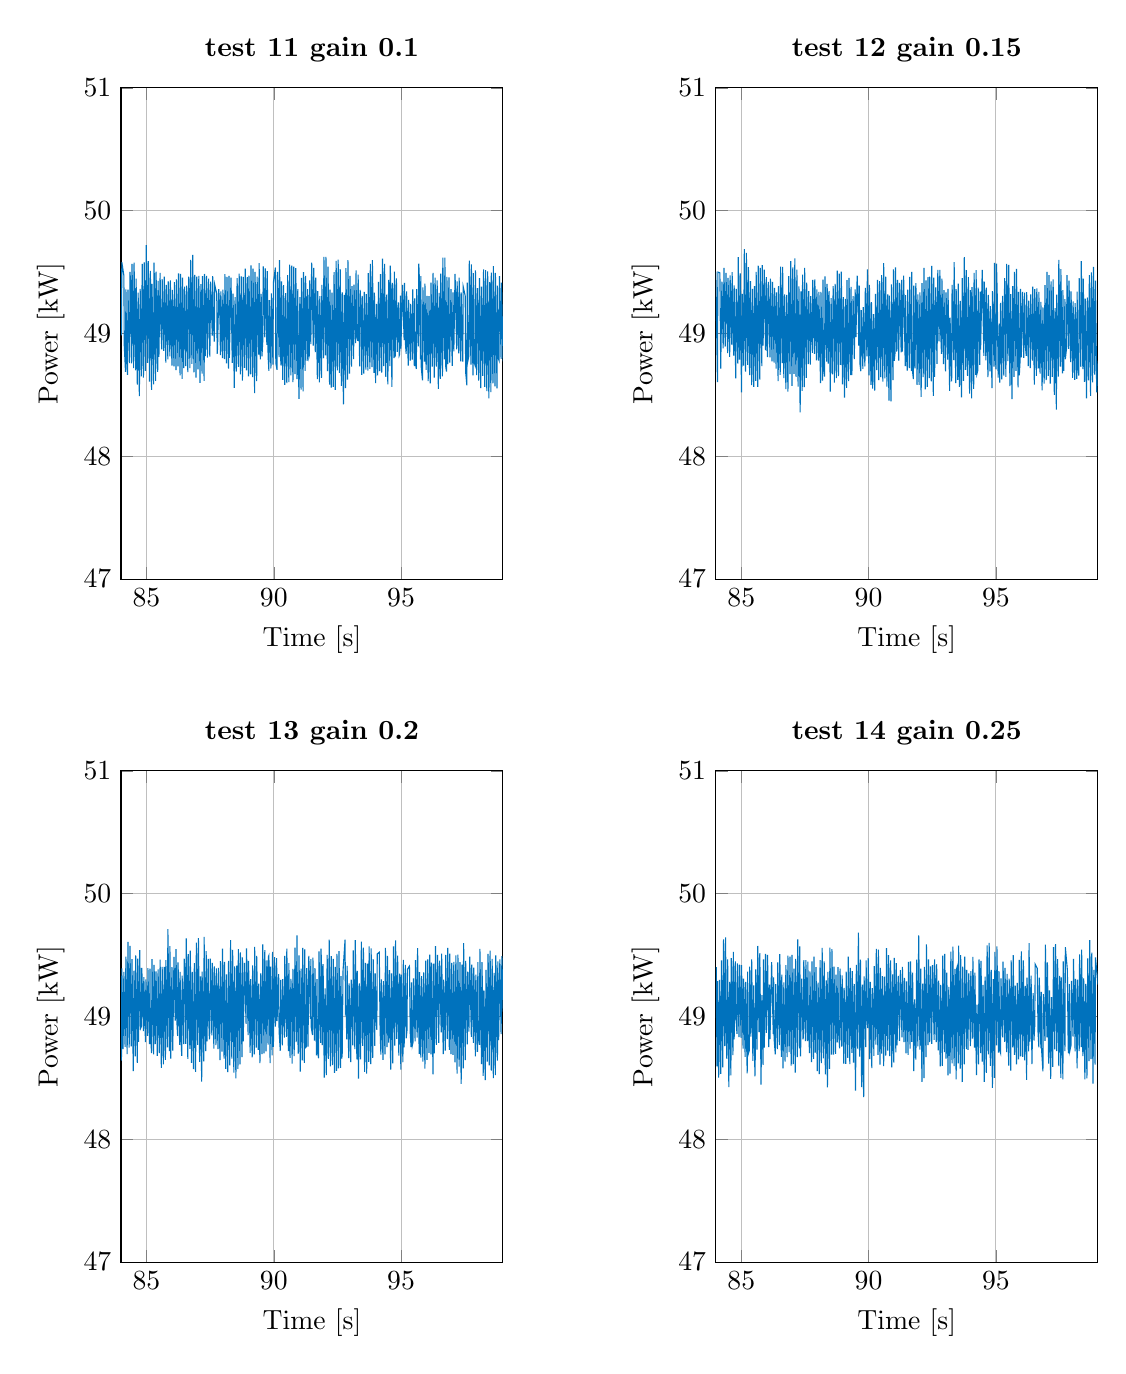
\begin{tikzpicture}

\begin{axis}[%
width=0.4\textwidth,
height=2.456in,
at={(1.026in,4.208in)},
scale only axis,
xmin=84,
xmax=99,
xlabel={Time [s]},
xmajorgrids,
ymin=47,
ymax=51,
ylabel={Power [kW]},
ymajorgrids,
axis background/.style={fill=white},
title style={font=\bfseries},
title={test 11 gain 0.1}
]
\addplot [color=mycolor1,solid,forget plot]
  table[row sep=crcr]{%
84	49.0169089058505\\
84.016	48.9844748267889\\
84.032	49.5802247060986\\
84.112	49.4717245805939\\
84.128	48.900872707621\\
84.176	48.6864423092357\\
84.192	49.3597079895846\\
84.224	48.80893808381\\
84.256	48.6635207858564\\
84.272	49.357010188079\\
84.336	48.7586612070903\\
84.352	49.5006541449799\\
84.384	49.385519653654\\
84.416	48.7572848925376\\
84.432	49.5659791307668\\
84.496	48.7186399764916\\
84.512	49.5770671584779\\
84.576	48.7005075356177\\
84.592	49.4470210163166\\
84.64	48.5829178793264\\
84.672	49.3333052727512\\
84.72	48.4894720132657\\
84.752	49.3622901109422\\
84.8	48.6509133555763\\
84.832	49.5661944269444\\
84.88	48.6410250361953\\
84.912	49.5779282193372\\
84.96	48.6944886151804\\
84.992	49.7198765936958\\
85.04	48.7609393066397\\
85.072	49.5898466619103\\
85.12	48.6076538132019\\
85.152	49.5087208667812\\
85.184	48.9253423225363\\
85.2	48.5401979662001\\
85.216	49.4045199113039\\
85.28	48.5854064115594\\
85.296	49.5764530072346\\
85.312	49.3788710427791\\
85.36	48.6130498963857\\
85.376	49.5041372011702\\
85.44	48.6863821274967\\
85.456	49.428933762495\\
85.488	48.8092228356552\\
85.536	49.4925145684949\\
85.552	49.1305104072367\\
85.6	48.8701252743407\\
85.616	49.4432529713372\\
85.68	48.8577891719177\\
85.696	49.4625970268877\\
85.76	48.7626985672674\\
85.776	49.3947273169067\\
85.84	48.7894020253203\\
85.856	49.4236294780404\\
85.92	48.8134848205511\\
85.936	49.4320915082136\\
86	48.7375072946178\\
86.016	49.3541088013669\\
86.08	48.7321047462098\\
86.096	49.4182280201765\\
86.16	48.7013732284729\\
86.176	49.4399707843508\\
86.24	48.7318943621212\\
86.256	49.4901631201156\\
86.32	48.6596866936168\\
86.336	49.4853536885241\\
86.4	48.6311120615644\\
86.416	49.4548372499486\\
86.464	48.7185634007819\\
86.496	49.38192382194\\
86.544	48.7341821565191\\
86.576	49.3898815727\\
86.624	48.6846937549129\\
86.656	49.4619940059908\\
86.688	49.208233097244\\
86.704	48.7185166486584\\
86.736	49.5985400370416\\
86.784	48.7521102475297\\
86.816	49.6390398107907\\
86.864	48.6831985189323\\
86.896	49.4762477016854\\
86.944	48.6404524360398\\
86.976	49.4620488107665\\
87.024	48.7076339396806\\
87.056	49.4686475962203\\
87.104	48.597658562259\\
87.136	49.4022104828018\\
87.184	48.6724440242871\\
87.2	49.4667353834394\\
87.264	48.6147876189793\\
87.28	49.484240678182\\
87.312	48.8153259672411\\
87.36	49.4696769591773\\
87.392	48.8024006215253\\
87.44	49.4474124530619\\
87.488	48.8108830555769\\
87.52	49.4228971231149\\
87.584	48.9826620879788\\
87.6	49.4664007902291\\
87.632	49.0726326002477\\
87.664	48.933233887961\\
87.68	49.3967027805484\\
87.76	49.3236454915286\\
87.776	48.8347951894554\\
87.792	48.8807635429971\\
87.84	49.3616372287831\\
87.888	49.1021959845568\\
87.904	48.8232557097564\\
87.92	49.3418875691544\\
87.984	48.7995739415514\\
88	49.3568180356585\\
88.064	48.7919350071699\\
88.08	49.4825507633881\\
88.144	48.7566272918963\\
88.16	49.4605279489163\\
88.224	48.7133218493312\\
88.24	49.4695213168452\\
88.256	48.8022243518374\\
88.32	49.4546009185058\\
88.368	48.7598524922647\\
88.384	48.8499389778292\\
88.4	49.3243822132179\\
88.448	48.5560125135762\\
88.48	49.2959245542207\\
88.528	48.6903352380271\\
88.56	49.4500332597027\\
88.608	48.7287687697226\\
88.64	49.4879277292949\\
88.672	48.9947520293556\\
88.688	48.6674436447754\\
88.72	49.4650307458113\\
88.768	48.6161290987339\\
88.8	49.4600519540393\\
88.848	48.7195139469931\\
88.88	49.5272735858181\\
88.928	48.698834671546\\
88.96	49.4580241662615\\
89.008	48.6503173295521\\
89.024	49.470309583434\\
89.088	48.6679097705205\\
89.104	49.554381487247\\
89.168	48.6442878994423\\
89.184	49.5281138448785\\
89.248	48.5139101628815\\
89.264	49.5011357549784\\
89.328	48.6118005727026\\
89.344	49.4624471803879\\
89.408	48.8275145962253\\
89.424	49.5734029694482\\
89.472	48.7893911690877\\
89.504	49.3223363192595\\
89.536	48.8140695034152\\
89.568	48.9426771460025\\
89.584	49.5467509303359\\
89.648	48.9678534791199\\
89.664	49.5307137288475\\
89.728	48.9077969376491\\
89.744	49.5080466937978\\
89.776	48.8194089485116\\
89.808	48.6958204379744\\
89.824	49.2717007836616\\
89.888	48.7147955584784\\
89.904	49.326134895352\\
89.936	49.0384376076761\\
89.968	48.7454951217813\\
89.984	49.4130715886081\\
90.064	49.5368941237885\\
90.08	48.7605310447507\\
90.128	48.7032769094771\\
90.144	49.5020063759187\\
90.176	49.2836838686221\\
90.208	48.8072297366825\\
90.224	49.5966566118936\\
90.272	48.7866773807604\\
90.288	48.737641198242\\
90.304	49.423634155987\\
90.352	48.6223125202158\\
90.384	49.3934493294029\\
90.432	48.5820612974277\\
90.464	49.3293849657853\\
90.512	48.5959791361397\\
90.544	49.475373921571\\
90.592	48.6037094531114\\
90.624	49.5606776925079\\
90.672	48.6591084142611\\
90.704	49.5525776042074\\
90.736	48.8620805830979\\
90.752	48.6037875058024\\
90.784	49.5444054414426\\
90.832	48.6692478409677\\
90.864	49.5316959080661\\
90.912	48.6274802109532\\
90.944	49.3606211205599\\
90.96	48.7954553466286\\
90.992	48.4670269286919\\
91.024	49.2960983225291\\
91.072	48.5429390133263\\
91.088	49.4518370531392\\
91.104	49.2362768110439\\
91.152	48.528147561417\\
91.168	49.5001656512308\\
91.232	48.6951223956669\\
91.248	49.4681320989166\\
91.312	48.7768403983766\\
91.328	49.3604822418058\\
91.376	48.8047160325891\\
91.392	48.8180407267962\\
91.408	49.4318313610728\\
91.456	48.9123056702117\\
91.488	49.5777353179128\\
91.552	48.9014157073445\\
91.568	49.5332945060032\\
91.632	48.847127080541\\
91.648	49.4541698204435\\
91.712	48.6283122299928\\
91.728	49.3453603193346\\
91.792	48.6008412975471\\
91.808	49.3043919866098\\
91.872	48.6390895223832\\
91.888	49.3950515959465\\
91.952	48.7982461230206\\
91.968	49.6230911640805\\
92.032	48.8206684039795\\
92.048	49.6238120421156\\
92.096	48.8537917836681\\
92.112	48.6924062995921\\
92.128	49.5437588138977\\
92.192	48.5831075947955\\
92.208	49.357646067092\\
92.256	48.5583703315639\\
92.288	49.3321544101335\\
92.336	48.5649008611993\\
92.368	49.4989968975274\\
92.416	48.539795908261\\
92.448	49.5903139595197\\
92.48	49.0364871433605\\
92.496	48.6986222939083\\
92.528	49.60093154951\\
92.576	48.6794298532157\\
92.608	49.524899428246\\
92.656	48.5727182667885\\
92.688	49.3351711572891\\
92.736	48.4226185122326\\
92.768	49.3151456236219\\
92.816	48.5542500624936\\
92.832	49.5320231164491\\
92.896	48.6238158098585\\
92.912	49.5979579974473\\
92.976	48.6726240257222\\
92.992	49.4685492764782\\
93.056	48.7307214486952\\
93.072	49.3864395894595\\
93.136	48.7915184388296\\
93.152	49.3986179278113\\
93.216	48.9206353235862\\
93.232	49.5145305481237\\
93.248	48.9908329703218\\
93.296	48.9400988823116\\
93.312	49.479616606497\\
93.376	48.7326292243011\\
93.392	49.3553913310667\\
93.44	49.0886904693646\\
93.456	48.6631202377438\\
93.472	49.306380177736\\
93.536	48.6731673086964\\
93.552	49.3378028647713\\
93.616	48.7064268958383\\
93.632	49.3209157018033\\
93.696	48.6967836342588\\
93.712	49.4903775704988\\
93.776	48.711323758838\\
93.792	49.56648278276\\
93.856	48.7264527024536\\
93.872	49.5971343445429\\
93.936	48.6782446334458\\
93.952	49.33183873678\\
94	48.5947815798052\\
94.032	49.2413958681192\\
94.08	48.6583619119988\\
94.112	49.4209391527211\\
94.16	48.693578802542\\
94.176	49.0139854983959\\
94.192	49.4832755147433\\
94.24	48.6821842173762\\
94.272	49.6090872430614\\
94.32	48.7345530738428\\
94.352	49.5657265096742\\
94.4	48.6471671682381\\
94.432	49.3165170364057\\
94.48	48.5853014107502\\
94.512	49.4362359483689\\
94.56	48.7342948879662\\
94.576	49.5529269853516\\
94.592	49.3976251254366\\
94.64	48.5651963661569\\
94.656	49.4124032127145\\
94.72	48.7986092411523\\
94.736	49.5030137174826\\
94.768	48.8067882134988\\
94.816	49.448858886669\\
94.848	48.8499427985828\\
94.896	49.2538372902447\\
94.928	48.82196606186\\
94.944	48.8315912242429\\
94.976	49.3080664116005\\
94.992	48.8766433072374\\
95.056	49.3959519348052\\
95.12	48.9450440578163\\
95.136	49.4124173813327\\
95.168	48.9282934198917\\
95.2	48.8334817045945\\
95.216	49.3430578441644\\
95.28	48.7373911044127\\
95.296	49.2728543421876\\
95.36	48.7785890882779\\
95.376	49.2417803984554\\
95.44	48.7872357722384\\
95.456	49.3592456304037\\
95.52	48.7338835637343\\
95.536	49.2867399983707\\
95.552	48.7661687892377\\
95.6	48.7110653245937\\
95.616	49.3609720308292\\
95.68	48.8958242676996\\
95.696	49.5690770105231\\
95.728	49.3847976396151\\
95.76	48.7894658570646\\
95.776	49.4665155720479\\
95.792	48.7275247881959\\
95.84	48.6189418664981\\
95.856	49.3762284421884\\
95.92	48.7714008588095\\
95.936	49.4061910223326\\
95.984	48.7028685960292\\
96.016	49.3063726690264\\
96.064	48.6127640497808\\
96.096	49.3046080468432\\
96.144	48.5944767780084\\
96.176	49.414619987902\\
96.224	48.7310035168073\\
96.256	49.4930275419816\\
96.304	48.6405490244419\\
96.336	49.4556796435888\\
96.384	48.7308739012485\\
96.416	49.4318445448527\\
96.464	48.5489531580649\\
96.496	49.3297109694216\\
96.512	48.8173301399231\\
96.544	48.6307420763667\\
96.56	49.4880817306332\\
96.624	48.6497514897525\\
96.64	49.6171029534225\\
96.656	49.3056046635091\\
96.704	48.7898205883149\\
96.72	49.6180450859425\\
96.752	48.7321064229018\\
96.784	48.689319699369\\
96.8	49.4607667511971\\
96.832	48.7505770867786\\
96.88	49.4571174152758\\
96.896	48.9682525772699\\
96.912	48.763408394661\\
96.96	49.3616074903946\\
97.008	48.7366974142742\\
97.04	49.33397550213\\
97.072	48.8532349120618\\
97.12	49.4852210877568\\
97.184	48.8706766983351\\
97.2	49.4233508043526\\
97.264	48.8386132092746\\
97.28	49.4543729155326\\
97.344	48.772376490165\\
97.36	49.334508358389\\
97.424	48.7711677260758\\
97.44	49.3811099755597\\
97.52	49.3048014530772\\
97.536	48.6855099493057\\
97.584	48.5780703254334\\
97.6	49.4130241451009\\
97.616	48.7687390929984\\
97.664	48.8185784728687\\
97.68	49.5929325378697\\
97.744	48.7454209250498\\
97.76	49.5630013386401\\
97.824	48.6587296498432\\
97.84	49.4922802084271\\
97.856	48.7766691673055\\
97.904	48.7423680408421\\
97.92	49.5135901492591\\
97.968	48.6600895008355\\
98	49.3686847452885\\
98.032	49.0370998384929\\
98.048	48.6157594531927\\
98.08	49.4504916502091\\
98.128	48.5548904131815\\
98.16	49.3814362808141\\
98.208	48.655166467765\\
98.24	49.52206064808\\
98.288	48.5646700970269\\
98.32	49.5159168201201\\
98.368	48.5298313360615\\
98.4	49.5057545546078\\
98.448	48.4718790841808\\
98.48	49.4173947258891\\
98.528	48.5228197623924\\
98.544	49.4949696259498\\
98.608	48.5934992288887\\
98.624	49.5478892316835\\
98.688	48.5701735269082\\
98.704	49.4927162637539\\
98.768	48.5537174187022\\
98.784	49.3893134384493\\
98.816	48.797975170701\\
98.848	48.7800652186248\\
98.864	49.4671998801087\\
98.928	48.7926416901304\\
98.944	49.4134172426027\\
99.008	48.7722302284671\\
};
\end{axis}

\begin{axis}[%
width=0.4\textwidth,
height=2.456in,
at={(4in,4.208in)},
scale only axis,
xmin=84,
xmax=99,
xlabel={Time [s]},
xmajorgrids,
ymin=47,
ymax=51,
ylabel={Power [kW]},
ymajorgrids,
axis background/.style={fill=white},
title style={font=\bfseries},
title={test 12  gain 0.15}
]
\addplot [color=mycolor1,solid,forget plot]
  table[row sep=crcr]{%
84	49.5038069907064\\
84.064	48.6037440935047\\
84.08	49.499825776313\\
84.16	49.4939301398254\\
84.192	48.7134794501232\\
84.24	49.4220975263013\\
84.288	48.8780459716874\\
84.32	49.533523893886\\
84.368	48.8935611354264\\
84.4	49.4937775462148\\
84.464	48.8399238701104\\
84.48	49.4533613809697\\
84.544	48.8095845308144\\
84.56	49.4739462793792\\
84.624	48.9101334303946\\
84.64	49.5000765260536\\
84.704	48.8204771608151\\
84.72	49.3915696126465\\
84.784	48.6334022737542\\
84.8	49.3640732539224\\
84.864	48.7552567083583\\
84.88	49.6215347002217\\
84.928	48.7867949677195\\
84.96	49.4894615027561\\
85.008	48.5203495164646\\
85.04	49.3217444038861\\
85.088	48.7378576691486\\
85.12	49.6867841482276\\
85.136	49.2664641083363\\
85.168	48.6898577944878\\
85.2	49.6569168800035\\
85.248	48.7448392438928\\
85.28	49.5411544984269\\
85.328	48.6605293054579\\
85.36	49.4252180602218\\
85.408	48.5796078865074\\
85.44	49.3633419861384\\
85.488	48.5655931090682\\
85.52	49.3857220640761\\
85.568	48.6137987140713\\
85.584	49.5023808831468\\
85.648	48.5643049681478\\
85.664	49.5532316411354\\
85.728	48.6248200867524\\
85.744	49.5338447194622\\
85.808	48.7334021083593\\
85.824	49.5562972206183\\
85.856	48.9010717224885\\
85.904	49.5193411441379\\
85.952	48.8701973790848\\
85.968	48.8673663599791\\
85.984	49.4584532508067\\
86.032	48.8076398869062\\
86.064	49.4193035288406\\
86.112	48.9707615255818\\
86.128	48.8062069889045\\
86.144	49.4469649467906\\
86.208	48.7722180156912\\
86.224	49.4206406468787\\
86.288	48.7634561628186\\
86.304	49.3719974502122\\
86.352	48.9834221625831\\
86.368	48.7133426766885\\
86.384	49.3339887931971\\
86.448	48.6124470806968\\
86.464	49.3845675818686\\
86.528	48.6619143142157\\
86.544	49.5443649712902\\
86.608	48.7593374721718\\
86.624	49.5418053905634\\
86.672	48.6365344343711\\
86.704	49.3178397746027\\
86.752	48.5472251261599\\
86.784	49.3144193433257\\
86.832	48.5259955495144\\
86.848	48.9961415246813\\
86.864	49.4659884311735\\
86.912	48.669431546344\\
86.944	49.5886141621949\\
86.992	48.5723482227499\\
87.024	49.5377387052814\\
87.072	48.6717049475625\\
87.104	49.6122219702913\\
87.12	48.9564815907084\\
87.152	48.6475677122742\\
87.184	49.5200989719598\\
87.232	48.5662628462146\\
87.264	49.3831518136921\\
87.312	48.3578233974264\\
87.344	49.3433047776039\\
87.392	48.5320016984337\\
87.408	49.4786069921407\\
87.472	48.5632028285811\\
87.488	49.5343865370033\\
87.552	48.6379418875242\\
87.568	49.4142986258413\\
87.632	48.7497403446026\\
87.648	49.3440304915919\\
87.712	48.7461450492346\\
87.728	49.3038973362061\\
87.792	48.8429480062172\\
87.808	49.436814366927\\
87.872	48.834258472144\\
87.888	49.4398577981217\\
87.952	48.7803825706986\\
87.968	49.3594830201525\\
88.032	48.779638466497\\
88.048	49.3379991471052\\
88.112	48.5962233936109\\
88.128	49.3394298513754\\
88.192	48.6154183101513\\
88.208	49.4375100066023\\
88.224	48.7422878138065\\
88.272	48.648928941953\\
88.288	49.4643444442604\\
88.352	48.7703296171172\\
88.368	49.4030648839136\\
88.4	49.2231980344715\\
88.416	48.7553355565064\\
88.448	49.3446536809606\\
88.496	48.5271481822455\\
88.528	49.2872961402541\\
88.576	48.6672762016391\\
88.608	49.3861611089357\\
88.64	49.0705463781486\\
88.656	48.6004317865256\\
88.688	49.4034540390119\\
88.736	48.6359074163237\\
88.768	49.5108098362135\\
88.816	48.6520011436039\\
88.848	49.4878021356038\\
88.896	48.7438781178968\\
88.928	49.5032249802012\\
88.976	48.5847863493606\\
89.008	49.2959915324401\\
89.056	48.4784951032926\\
89.088	49.2809416543583\\
89.136	48.5564417478976\\
89.152	49.4338280162826\\
89.184	48.8118982272855\\
89.216	48.6115626316357\\
89.232	49.4518142103971\\
89.296	48.6598403236941\\
89.312	49.3801040992184\\
89.344	48.66045609063\\
89.392	49.3050069261441\\
89.44	48.7909222890525\\
89.472	49.3598712285422\\
89.504	48.9695766888491\\
89.552	49.4718654195972\\
89.6	49.1262147661018\\
89.616	48.9003848939715\\
89.632	49.3888523334038\\
89.664	48.7493037061966\\
89.696	48.6926374568389\\
89.712	49.1893885668751\\
89.776	48.71106155167\\
89.792	49.2153150260556\\
89.856	48.7311141390742\\
89.872	49.3716064991573\\
89.936	48.8142387927897\\
89.952	49.5223404263742\\
90.016	48.6580194152353\\
90.032	49.3950395279427\\
90.096	48.5814440836091\\
90.112	49.2542311004314\\
90.16	48.5506183351229\\
90.192	49.1572360020327\\
90.24	48.5336699373483\\
90.272	49.323070558222\\
90.32	48.702306600312\\
90.336	49.0552506004141\\
90.352	49.4370787624979\\
90.4	48.6208739459444\\
90.432	49.4256489063425\\
90.48	48.6437636202621\\
90.512	49.4752420332938\\
90.56	48.6088560182668\\
90.592	49.5719523035987\\
90.64	48.6342595753614\\
90.672	49.4637343200456\\
90.72	48.5666452519028\\
90.736	49.1036807623544\\
90.752	49.3186285013683\\
90.8	48.4525330797042\\
90.816	49.3074064052811\\
90.88	48.4461730181163\\
90.896	49.4001533636783\\
90.96	48.6209999761955\\
90.976	49.5213297626982\\
91.008	48.7768710679784\\
91.04	48.8437457104153\\
91.056	49.5376954105982\\
91.104	48.8524316671231\\
91.136	49.4367357102118\\
91.184	48.7787290583499\\
91.216	49.4117509194635\\
91.28	48.8468225931853\\
91.296	49.4356214852866\\
91.328	48.8528306007749\\
91.376	49.4718303777153\\
91.44	48.7349058032405\\
91.456	49.3118582247748\\
91.472	48.8811105646462\\
91.52	48.6973776713163\\
91.536	49.3578791864364\\
91.6	48.7186578910662\\
91.616	49.4604562321205\\
91.68	48.6945509591088\\
91.696	49.5022873724309\\
91.712	48.7165387421648\\
91.76	48.6276888023596\\
91.776	49.3898736292064\\
91.824	48.7163776766137\\
91.856	49.4099075641525\\
91.888	49.1060047936309\\
91.904	48.5811908094178\\
91.936	49.3190431732216\\
91.984	48.5818353731345\\
92.016	49.3346974898261\\
92.064	48.4842929476451\\
92.096	49.4108598741465\\
92.144	48.644227415841\\
92.176	49.5335595729859\\
92.224	48.5441111804734\\
92.256	49.4327673192463\\
92.304	48.5644205488471\\
92.336	49.4594630409104\\
92.384	48.6372492366787\\
92.4	49.4620570499638\\
92.464	48.6105863923247\\
92.48	49.5495621817775\\
92.544	48.4922696539267\\
92.56	49.4546458843938\\
92.592	48.6465773387439\\
92.64	49.3761680466695\\
92.688	48.751609093197\\
92.72	49.5170071757899\\
92.768	48.9363165657829\\
92.8	49.5169280956645\\
92.832	49.0093428157276\\
92.864	48.834298668536\\
92.88	49.4473133258807\\
92.944	48.7502339338664\\
92.96	49.353166150084\\
93.024	48.6914728936672\\
93.04	49.3341830402074\\
93.088	49.0724015507293\\
93.104	48.7878234107006\\
93.12	49.3635131810734\\
93.184	48.5328937673568\\
93.2	49.1279208468092\\
93.264	48.6106997525727\\
93.28	49.3960718157219\\
93.344	48.783437675396\\
93.36	49.5810458101683\\
93.424	48.5963795418176\\
93.44	49.3619560084691\\
93.504	48.6225142280705\\
93.52	49.4059092581361\\
93.568	48.5646679368748\\
93.584	48.7746833038467\\
93.6	49.2645238058753\\
93.648	48.4788299318156\\
93.68	49.4500535903226\\
93.728	48.6130848857711\\
93.76	49.6226605185011\\
93.808	48.7026299543524\\
93.84	49.5156764909125\\
93.856	48.8855325058665\\
93.888	48.6544819013259\\
93.92	49.4593044294598\\
93.968	48.5095479910815\\
94	49.3533081313517\\
94.048	48.4721170683856\\
94.064	49.3770391428968\\
94.128	48.5482242009354\\
94.144	49.4930225636126\\
94.208	48.6633638059663\\
94.224	49.5157126508689\\
94.256	48.6714947913721\\
94.288	48.6975632982284\\
94.304	49.3737102919915\\
94.368	48.7450351621596\\
94.384	49.3402501330944\\
94.4	48.8688142962821\\
94.464	49.5185369207961\\
94.528	48.8171324188631\\
94.544	49.4218141007495\\
94.608	48.7800539058591\\
94.624	49.3727594513491\\
94.688	48.6447980652742\\
94.704	49.3145216880092\\
94.768	48.6909224446663\\
94.784	49.223211587932\\
94.848	48.5545864578216\\
94.864	49.3452703365447\\
94.928	48.7306549579658\\
94.944	49.5748335311221\\
94.96	48.8648019377479\\
95.008	48.7084282486815\\
95.024	49.5686747306093\\
95.056	49.2862090629255\\
95.088	48.6402634904717\\
95.136	49.0801240985127\\
95.152	48.6001652496371\\
95.184	49.2494292865453\\
95.232	48.6271658675141\\
95.264	49.3063032967745\\
95.312	48.6558553406629\\
95.344	49.4500994435121\\
95.376	49.0998294116104\\
95.392	48.6466286461453\\
95.424	49.5657235042507\\
95.472	48.774381001367\\
95.504	49.5587794550036\\
95.552	48.5710332500356\\
95.584	49.3204610317875\\
95.632	48.4647236840711\\
95.664	49.3851921065805\\
95.712	48.6456372883313\\
95.728	49.5015485434429\\
95.792	48.6962462970608\\
95.808	49.5261118849367\\
95.872	48.5602502817271\\
95.888	49.3388275701979\\
95.92	48.6593945849362\\
95.952	48.7833927121535\\
95.968	49.3633347869409\\
96	48.8046113529439\\
96.048	49.3378442314965\\
96.096	48.8011616570995\\
96.128	49.3316976890176\\
96.144	48.9336835492124\\
96.192	48.8184064037066\\
96.208	49.3356447147723\\
96.272	48.7349803021293\\
96.288	49.2681065615042\\
96.336	48.9907966577278\\
96.352	48.7171463325596\\
96.368	49.3185639121857\\
96.432	48.7782576428617\\
96.448	49.3820638477661\\
96.512	48.5841477601296\\
96.528	49.3615779667609\\
96.592	48.6550469150258\\
96.608	49.3676348450661\\
96.672	48.716057492659\\
96.688	49.338978351368\\
96.736	48.6733450618631\\
96.768	49.2572268729981\\
96.816	48.5366133805674\\
96.848	49.2124518849859\\
96.896	48.5913499404567\\
96.928	49.3937732952701\\
96.976	48.620391493485\\
97.008	49.501424858931\\
97.056	48.6542608433416\\
97.088	49.4748578785338\\
97.12	48.8078813757669\\
97.136	48.5916664044194\\
97.168	49.4238628021699\\
97.216	48.6458739545148\\
97.248	49.4403402483909\\
97.296	48.4995094255828\\
97.328	49.2055028246513\\
97.376	48.3798062458935\\
97.392	49.3159016678968\\
97.456	48.6495930919019\\
97.472	49.5990841341864\\
97.536	48.7299229208156\\
97.552	49.5231128352725\\
97.616	48.6742023695223\\
97.632	49.353796361151\\
97.664	48.6957127247172\\
97.712	49.279513247792\\
97.728	48.7904139153312\\
97.776	48.8818299838418\\
97.792	49.4747983715065\\
97.856	48.8741864979219\\
97.872	49.4304095332399\\
97.936	48.7660932269944\\
97.952	49.3421496524405\\
98.016	48.6394305795144\\
98.032	49.2602740475986\\
98.096	48.6214537348432\\
98.112	49.246814944602\\
98.176	48.6310920654469\\
98.192	49.3404502953179\\
98.208	48.7635271055831\\
98.256	48.65777630968\\
98.272	49.4513331315759\\
98.336	48.72814283674\\
98.352	49.5899601234167\\
98.416	48.7092326830475\\
98.432	49.4470192662438\\
98.48	48.6052002584493\\
98.512	49.2834189182021\\
98.56	48.4721663125039\\
98.592	49.2927552425023\\
98.624	49.107233137744\\
98.64	48.6180425148641\\
98.672	49.4748801101143\\
98.72	48.490944582343\\
98.752	49.4983917145101\\
98.8	48.6013695251837\\
98.832	49.5418598353966\\
98.88	48.6642420585601\\
98.912	49.4300353039572\\
98.96	48.521335498098\\
99.008	48.7795805409579\\
};
\end{axis}

\begin{axis}[%
width=0.4\textwidth,
height=2.456in,
at={(1.026in,0.793in)},
scale only axis,
xmin=84,
xmax=99,
xlabel={Time [s]},
xmajorgrids,
ymin=47,
ymax=51,
ylabel={Power [kW]},
ymajorgrids,
axis background/.style={fill=white},
title style={font=\bfseries},
title={test 13  gain 0.2}
]
\addplot [color=mycolor1,solid,forget plot]
  table[row sep=crcr]{%
84	48.815894737406\\
84.016	48.6398090761449\\
84.032	49.3920870288813\\
84.08	48.7351100557408\\
84.112	49.362493377366\\
84.16	48.7516003912645\\
84.192	49.4878962207364\\
84.24	48.6940872090645\\
84.272	49.6075158464323\\
84.32	48.7462550026138\\
84.352	49.5751328163386\\
84.4	48.7557836329323\\
84.416	49.0131403645153\\
84.432	49.4663388254043\\
84.48	48.5553058811619\\
84.512	49.3725322378995\\
84.56	48.6759797991608\\
84.576	49.4966999720792\\
84.64	48.6217302008458\\
84.656	49.4717371102187\\
84.688	48.7939427408081\\
84.736	49.5405531971613\\
84.768	48.9031466996863\\
84.8	48.9174253594289\\
84.816	49.3952172353794\\
84.88	48.8803368984673\\
84.896	49.320915700733\\
84.96	48.7905082216155\\
84.976	49.3024416529556\\
85.04	48.842516292072\\
85.056	49.3930127807198\\
85.12	48.7753232264881\\
85.136	49.389287352475\\
85.152	48.873271348612\\
85.2	48.7023268694526\\
85.216	49.4662243642328\\
85.28	48.6905057342956\\
85.296	49.4206994618577\\
85.328	49.1746816491057\\
85.344	48.7738671206946\\
85.376	49.3671078989093\\
85.424	48.6787106724785\\
85.456	49.3834825167506\\
85.504	48.7011759754881\\
85.536	49.4626423059309\\
85.552	49.1073264362879\\
85.584	48.5816046403558\\
85.616	49.4032074712733\\
85.664	48.6101985424491\\
85.696	49.4042364216365\\
85.744	48.6461643703924\\
85.76	49.4592422179754\\
85.824	48.7479685041804\\
85.84	49.7121241760729\\
85.904	48.7177515005119\\
85.92	49.5724394788415\\
85.952	48.6559094121242\\
86	49.4012296441303\\
86.032	48.7211409626807\\
86.08	49.4848613043468\\
86.128	48.9657397607849\\
86.16	49.547378650794\\
86.192	48.9640184360826\\
86.224	48.8411791529589\\
86.24	49.4408973168434\\
86.304	48.7689423611629\\
86.32	49.3627645791218\\
86.352	48.8443094838128\\
86.384	48.6801207372826\\
86.4	49.3321201983036\\
86.464	48.7751864435502\\
86.48	49.4707279005347\\
86.512	49.3686704996845\\
86.544	48.7778355857644\\
86.56	49.6367105013804\\
86.624	48.65520466093\\
86.64	49.507773751448\\
86.704	48.737002073904\\
86.72	49.535580724495\\
86.768	48.6226387969055\\
86.8	49.3629047961709\\
86.848	48.5706328188966\\
86.88	49.4345456858998\\
86.928	48.5492521500416\\
86.96	49.600868293722\\
87.008	48.7691460178972\\
87.04	49.6382354791895\\
87.088	48.6311317554113\\
87.12	49.3265082456406\\
87.168	48.4687436327377\\
87.184	49.3650091533555\\
87.248	48.6345240421927\\
87.264	49.6488703903869\\
87.296	48.9402007616968\\
87.328	48.7174541259907\\
87.344	49.5326143531416\\
87.376	48.7966461733277\\
87.424	49.4692638509727\\
87.44	49.0104563790863\\
87.472	48.8143387646252\\
87.488	48.8785554822543\\
87.504	49.4710074937506\\
87.568	48.845783253672\\
87.584	49.4353854352469\\
87.648	48.7375530475832\\
87.664	49.4070251186706\\
87.728	48.7660062361539\\
87.744	49.3923049632971\\
87.808	48.7350632743362\\
87.824	49.3946661523693\\
87.888	48.6449892139502\\
87.904	49.4512031775877\\
87.968	48.7147205242317\\
87.984	49.5529545820522\\
88.048	48.657644368048\\
88.064	49.4444058738086\\
88.112	48.5730214268433\\
88.144	49.3418288960945\\
88.192	48.547352259858\\
88.208	48.9208862852633\\
88.224	49.4531735190772\\
88.272	48.6025692292644\\
88.304	49.620935324388\\
88.352	48.6566215220971\\
88.384	49.5430418548482\\
88.432	48.5425863410752\\
88.464	49.4086835967253\\
88.512	48.4951637027408\\
88.544	49.4143180121526\\
88.592	48.5732044834039\\
88.608	49.5488546963892\\
88.624	49.4163803892088\\
88.672	48.6094556284808\\
88.688	49.5221533744795\\
88.752	48.6686207470824\\
88.768	49.4819668108103\\
88.8	48.7977001360339\\
88.848	49.4367107506111\\
88.912	48.9406792901463\\
88.928	49.5542001055971\\
88.992	48.8488025775875\\
89.008	49.4526715370446\\
89.072	48.7026589304267\\
89.088	49.303795875708\\
89.152	48.6670510619646\\
89.168	49.4161259894388\\
89.232	48.6913540393556\\
89.248	49.5660483300539\\
89.312	48.7460301678929\\
89.328	49.493704095979\\
89.392	48.7288340456126\\
89.408	49.2674458448712\\
89.456	48.6199631984966\\
89.488	49.3514343106385\\
89.536	48.6929663525616\\
89.568	49.586891695907\\
89.616	48.6997350534201\\
89.648	49.5401784970686\\
89.696	48.7163472994981\\
89.728	49.4572907581813\\
89.776	48.7698686723067\\
89.792	49.4865863354342\\
89.808	49.4956887119451\\
89.856	48.6202777009057\\
89.872	49.4057754622699\\
89.936	48.6832384011319\\
89.952	49.5252147243947\\
89.984	48.7528595280648\\
90.032	49.4826989536556\\
90.064	48.9173644625555\\
90.112	49.4755627109473\\
90.128	48.9631604025817\\
90.192	49.3450869262103\\
90.208	48.8810249508771\\
90.256	48.7210034595771\\
90.272	49.2979072535082\\
90.336	48.76413698126\\
90.352	49.3049960042267\\
90.416	48.8268591052689\\
90.432	49.4927811996191\\
90.496	48.8343764501156\\
90.512	49.5524469175711\\
90.56	48.8438192892013\\
90.576	48.7176260599446\\
90.592	49.4349167677836\\
90.64	48.6628544656026\\
90.672	49.3068090556792\\
90.704	49.0898693137769\\
90.72	48.6153105351161\\
90.752	49.3874610520021\\
90.8	48.6772466794177\\
90.832	49.5615588841074\\
90.88	48.7901157519638\\
90.912	49.6610455341207\\
90.928	49.0355832402729\\
90.96	48.6981106326281\\
90.992	49.4980307409164\\
91.04	48.5507422746587\\
91.072	49.3904494133116\\
91.12	48.6424005138926\\
91.136	49.5592482939366\\
91.2	48.6215930518869\\
91.216	49.5472290345373\\
91.248	48.7461800246955\\
91.28	48.7527803628941\\
91.296	49.3938357009724\\
91.344	48.7540604558232\\
91.376	49.4928648868985\\
91.44	48.9798011178607\\
91.456	49.4678780927219\\
91.472	48.911907850837\\
91.52	48.8494374738046\\
91.536	49.4786792800484\\
91.6	48.8041104242102\\
91.616	49.3942626730112\\
91.68	48.6836207065195\\
91.696	49.3049378003454\\
91.712	48.7366759008236\\
91.76	48.660002505499\\
91.776	49.5309019512576\\
91.84	48.7857824286483\\
91.856	49.5523765943642\\
91.888	49.2984772730916\\
91.904	48.7657534838734\\
91.936	49.4254703840358\\
91.984	48.5010497503314\\
92.016	49.2287100161605\\
92.064	48.5223176100282\\
92.096	49.5015636843872\\
92.144	48.6555792722735\\
92.176	49.6267332128714\\
92.224	48.594450944812\\
92.256	49.4913551452079\\
92.304	48.6040243368076\\
92.336	49.4686790421955\\
92.384	48.5405981433807\\
92.416	49.4038763404872\\
92.464	48.5573196810525\\
92.48	49.5093856093985\\
92.544	48.5772364217581\\
92.56	49.5316590344213\\
92.624	48.581936916484\\
92.64	49.3287694653422\\
92.672	48.657540582566\\
92.688	48.7006902887193\\
92.72	49.37137169593\\
92.8	49.6262522106154\\
92.816	49.0364614703813\\
92.848	49.0696975805911\\
92.864	48.8129105621971\\
92.88	49.4120614598737\\
92.944	48.6608430201343\\
92.96	49.2692502931983\\
93.024	48.6291350565493\\
93.04	49.3003885788738\\
93.072	49.1947359524553\\
93.104	48.7639827613058\\
93.12	49.5374979491207\\
93.184	48.7343269045639\\
93.2	49.6207176530994\\
93.264	48.6508423579015\\
93.28	49.3705314126976\\
93.328	48.4948805918957\\
93.36	49.2704171024028\\
93.408	48.6504849312511\\
93.44	49.6095778017787\\
93.488	48.7604008559703\\
93.52	49.5600833285442\\
93.568	48.5497702806816\\
93.6	49.4362767280886\\
93.632	48.8866424488136\\
93.648	48.533814608292\\
93.68	49.4306169196091\\
93.728	48.6309546180103\\
93.744	49.5702113404581\\
93.808	48.6112427781634\\
93.824	49.5540565894678\\
93.856	48.8306752623758\\
93.888	48.663889915109\\
93.904	49.4672408556767\\
93.968	48.7603153344209\\
93.984	49.3500001050526\\
94.016	48.9814290335462\\
94.048	48.891456704587\\
94.064	49.5095579994481\\
94.144	49.522720790653\\
94.176	48.8883999005998\\
94.208	48.688522550948\\
94.224	49.30269055255\\
94.288	48.6458444699597\\
94.304	49.2874873135884\\
94.368	48.6915192624889\\
94.384	49.5577913809239\\
94.448	48.7513819853576\\
94.464	49.4940796501858\\
94.512	48.7861628208353\\
94.544	49.3776085841946\\
94.592	48.5663364464725\\
94.624	49.3498883039406\\
94.672	48.6176760419733\\
94.704	49.5705043946903\\
94.752	48.7620367126484\\
94.784	49.619414068154\\
94.816	48.9804196763233\\
94.832	48.8180651466166\\
94.864	49.4958161840429\\
94.912	48.6813233263866\\
94.944	49.3485116227262\\
94.992	48.5673333603492\\
95.008	49.3398148236933\\
95.072	48.6272439479555\\
95.088	49.4611484088234\\
95.12	48.7483721259815\\
95.168	49.4192052789963\\
95.2	48.8224806538749\\
95.232	48.8862936109438\\
95.248	49.3836247921429\\
95.328	49.409767671537\\
95.36	48.8656173446311\\
95.392	48.749846940105\\
95.408	49.2770755846584\\
95.44	48.7626537912952\\
95.472	48.7924122237348\\
95.488	49.310107763075\\
95.552	48.7977761441657\\
95.568	49.4588499369173\\
95.632	48.827635425392\\
95.648	49.5568742874643\\
95.712	48.6954520736637\\
95.728	49.3603434405416\\
95.776	48.6646178160794\\
95.808	49.3292629642833\\
95.856	48.6330363123269\\
95.888	49.3587434469792\\
95.936	48.5756151769064\\
95.968	49.4541270169995\\
96.016	48.645885995381\\
96.048	49.4649999723002\\
96.096	48.7030468297004\\
96.128	49.5031207739488\\
96.176	48.6913331983907\\
96.192	49.4378221516488\\
96.256	48.5275343160128\\
96.272	49.4302203097402\\
96.304	48.699949223394\\
96.352	49.5737250634171\\
96.384	48.769196413911\\
96.432	49.5016381751236\\
96.48	48.7850821380652\\
96.512	49.454756872619\\
96.576	48.8711252282395\\
96.592	49.5110990363685\\
96.656	48.6933293608411\\
96.672	49.299369888677\\
96.736	48.7211257432959\\
96.752	49.5023961104265\\
96.816	48.8160754166237\\
96.832	49.5582353912595\\
96.896	48.7272282034449\\
96.912	49.5119348063697\\
96.96	48.6925689265733\\
96.992	49.4370249853234\\
97.04	48.6864012988034\\
97.072	49.4455149477522\\
97.12	48.6255175656045\\
97.152	49.497761566661\\
97.2	48.5351395013689\\
97.232	49.5045080585514\\
97.28	48.5913380487755\\
97.296	48.9486303844477\\
97.312	49.4427707703007\\
97.36	48.4515139128443\\
97.392	49.4226193561211\\
97.44	48.5779366654839\\
97.456	49.5974692710759\\
97.52	48.6450660676806\\
97.536	49.4520074494734\\
97.6	48.7727014134875\\
97.616	49.3643090014052\\
97.664	48.8770766524973\\
97.696	49.4864381742815\\
97.76	48.8347548375926\\
97.776	49.4230474087092\\
97.84	48.7844639026779\\
97.856	49.397077795774\\
97.92	48.6754773875991\\
97.936	49.3405000135732\\
98	48.7111188525448\\
98.016	49.4418088788536\\
98.032	48.8518075888391\\
98.08	48.7688661750926\\
98.096	49.5512400310306\\
98.16	48.6122578549936\\
98.176	49.4427644585092\\
98.208	49.084872292753\\
98.224	48.5153409018373\\
98.256	49.2106681996339\\
98.304	48.4817065660712\\
98.336	49.3791404732512\\
98.384	48.6316522538577\\
98.416	49.5091409325967\\
98.448	49.1142344179351\\
98.464	48.6014882308433\\
98.496	49.535584639609\\
98.544	48.5594742020088\\
98.576	49.4684809200575\\
98.624	48.498426660714\\
98.656	49.3547256089687\\
98.704	48.5221988143257\\
98.72	49.496905448951\\
98.784	48.640398476938\\
98.8	49.4476485246965\\
98.832	48.8081331771483\\
98.88	49.4653880936351\\
98.928	48.8567976882505\\
98.96	49.4909270346724\\
99.008	49.0398072716987\\
};
\end{axis}

\begin{axis}[%
width=0.4\textwidth,
height=2.456in,
at={(4in,0.793in)},
scale only axis,
xmin=84,
xmax=99,
xlabel={Time [s]},
xmajorgrids,
ymin=47,
ymax=51,
ylabel={Power [kW]},
ymajorgrids,
axis background/.style={fill=white},
title style={font=\bfseries},
title={test 14  gain 0.25}
]
\addplot [color=mycolor1,solid,forget plot]
  table[row sep=crcr]{%
84	48.9860071637557\\
84.016	49.4009200771033\\
84.048	48.5927593745919\\
84.064	49.2881742632098\\
84.112	48.5017788952446\\
84.144	49.2983494585013\\
84.192	48.5323098393178\\
84.224	49.4565099041887\\
84.272	48.5846079894036\\
84.304	49.6277136250771\\
84.352	48.7580521206885\\
84.384	49.6441081246769\\
84.4	48.9847512596999\\
84.432	48.6551754453703\\
84.464	49.4642649805067\\
84.512	48.425323454377\\
84.544	49.2817744399234\\
84.592	48.5198528745925\\
84.608	49.4750458016964\\
84.672	48.6860796789764\\
84.688	49.5261803862278\\
84.72	48.8127075741138\\
84.768	49.4492787176007\\
84.784	49.006586980044\\
84.832	48.8588268164996\\
84.848	49.4313851858053\\
84.912	48.8318951349572\\
84.928	49.4221256283733\\
84.992	48.8260527297893\\
85.008	49.418440443604\\
85.072	48.7390697461069\\
85.088	49.3071371259858\\
85.152	48.6714201378806\\
85.168	49.2816885979374\\
85.232	48.5372837585272\\
85.248	49.365554158898\\
85.264	48.6870505514997\\
85.312	48.7202910568673\\
85.328	49.4057221184615\\
85.376	48.835297419385\\
85.408	49.4653502604519\\
85.456	48.6387159769143\\
85.488	49.2535659325336\\
85.536	48.5116722105017\\
85.552	48.7134251847434\\
85.568	49.3834388499502\\
85.616	48.7303587568756\\
85.648	49.573801368921\\
85.696	48.8729280943131\\
85.728	49.5159766939077\\
85.776	48.4459728693738\\
85.808	49.1736585284298\\
85.856	48.6049299431876\\
85.872	49.4649463006377\\
85.904	48.7455868416642\\
85.952	49.5097116523194\\
85.984	48.8663489143279\\
86.032	49.5017404059266\\
86.08	48.7501627119441\\
86.112	49.2592726261783\\
86.128	48.8163376974914\\
86.192	49.442908752549\\
86.256	48.8583443947974\\
86.272	49.3174883643005\\
86.288	48.8204723310558\\
86.336	48.6916016470281\\
86.352	49.263955752725\\
86.416	48.7343785346331\\
86.432	49.4402804128461\\
86.496	48.7662174065243\\
86.512	49.5079377455197\\
86.576	48.6717294926083\\
86.592	49.3405429672228\\
86.64	48.5774813347261\\
86.672	49.2773875619383\\
86.72	48.632628866566\\
86.752	49.4187832712426\\
86.8	48.6696880491086\\
86.832	49.4963556182834\\
86.848	49.1332385185215\\
86.88	48.7103783079783\\
86.912	49.4874215105387\\
86.96	48.6002950656429\\
86.992	49.501986024556\\
87.04	48.6109343262459\\
87.072	49.3901561919727\\
87.12	48.5426633186704\\
87.136	49.4685273371098\\
87.2	48.6695473936748\\
87.216	49.6273739995181\\
87.28	48.7406573471144\\
87.296	49.5698806493538\\
87.328	48.6741102633352\\
87.376	49.3078481677219\\
87.424	48.8133121441161\\
87.44	48.8358355215581\\
87.456	49.4596287440937\\
87.52	48.799669164662\\
87.536	49.4588976351882\\
87.6	48.7986106624162\\
87.616	49.4457151113174\\
87.632	48.9805837111109\\
87.68	48.7018565887966\\
87.696	49.3675094676936\\
87.76	48.6287637361916\\
87.776	49.4476863124579\\
87.84	48.654760577289\\
87.856	49.4881505875883\\
87.904	48.7051142249376\\
87.936	49.4016422628047\\
87.984	48.5551042067292\\
88.016	49.2762677179587\\
88.048	49.0155710902543\\
88.064	48.5312201240524\\
88.096	49.4580287409859\\
88.144	48.6191055543981\\
88.176	49.5587428373172\\
88.224	48.6581136454175\\
88.256	49.448038179558\\
88.304	48.5291336609671\\
88.336	49.2937800240998\\
88.384	48.423603751147\\
88.4	49.3637939037128\\
88.464	48.5740562357635\\
88.48	49.5602859189653\\
88.544	48.6890579246242\\
88.56	49.5484894500262\\
88.624	48.6884273589056\\
88.64	49.406000271738\\
88.704	48.6955914728341\\
88.72	49.3415437350983\\
88.768	48.7893218301463\\
88.8	49.4021970039062\\
88.816	48.8891776567291\\
88.864	48.7405267059951\\
88.88	49.3897795561958\\
88.944	48.7544631439233\\
88.96	49.3347700728483\\
89.008	48.947895673641\\
89.024	48.6156409468579\\
89.04	49.2334852108539\\
89.104	48.614780622524\\
89.12	49.3643685168723\\
89.184	48.6637024268608\\
89.2	49.4881605551417\\
89.264	48.6123465535133\\
89.28	49.3949831217325\\
89.344	48.7030000010113\\
89.36	49.3691093268843\\
89.408	48.6234757777322\\
89.44	49.2625413667556\\
89.488	48.3956950076673\\
89.52	49.419312916053\\
89.568	48.7390326854154\\
89.6	49.6827257008391\\
89.648	48.6728124665092\\
89.68	49.4627534928858\\
89.728	48.4248856962701\\
89.76	49.2585163527224\\
89.776	48.7192757523418\\
89.808	48.3439703074086\\
89.824	49.3261716738665\\
89.888	48.7508203428485\\
89.904	49.4567978190109\\
89.92	49.0546633803961\\
89.968	48.9060447331573\\
89.984	49.4748615730688\\
90.032	48.898647508315\\
90.048	48.65273119167\\
90.064	49.2826242831819\\
90.128	48.5784056229099\\
90.144	49.2298362673236\\
90.192	48.9964190078391\\
90.208	48.679353855764\\
90.224	49.4104416629745\\
90.288	48.7702644307961\\
90.304	49.5499075248219\\
90.368	48.6879604649369\\
90.384	49.5442605821706\\
90.448	48.607962701497\\
90.464	49.3953159641571\\
90.512	48.6967182231388\\
90.544	49.3284732651607\\
90.592	48.596363585638\\
90.624	49.3249304330553\\
90.672	48.6810813625237\\
90.688	48.9359690658924\\
90.704	49.5568490154324\\
90.752	48.7223630848801\\
90.784	49.4998807319067\\
90.832	48.6764067801741\\
90.864	49.4566563437647\\
90.912	48.5856005713243\\
90.944	49.3426413544084\\
90.96	48.8316926336733\\
90.992	48.6243917459959\\
91.008	49.4762705802877\\
91.072	48.7075229431875\\
91.088	49.4349566836403\\
91.104	49.0564044424848\\
91.12	48.7643764910403\\
91.168	49.3311480332846\\
91.216	48.8009415321806\\
91.248	49.37672101143\\
91.312	48.8300560552401\\
91.328	49.4037181036071\\
91.392	48.7918870452829\\
91.408	49.3144344647224\\
91.472	48.6986339301435\\
91.488	49.2857554383124\\
91.552	48.6876963994973\\
91.568	49.4444702198248\\
91.632	48.7377348426683\\
91.648	49.4484782940396\\
91.696	48.7925814390703\\
91.728	49.3571623548571\\
91.776	48.5557753990402\\
91.808	49.1383006395828\\
91.856	48.648964648681\\
91.872	48.9976155090593\\
91.888	49.463216309556\\
91.936	48.7569254203949\\
91.968	49.6596756689632\\
92.016	48.7295928998368\\
92.048	49.3888321759843\\
92.096	48.468152541709\\
92.128	49.2676896548846\\
92.176	48.4974469963694\\
92.192	49.4037935125172\\
92.256	48.6680974198668\\
92.272	49.5870616673493\\
92.288	49.2160271503338\\
92.336	48.7663419653557\\
92.352	49.4654710107805\\
92.4	48.7918870172418\\
92.432	49.4079265621032\\
92.48	48.7764974378024\\
92.512	49.4184122868157\\
92.576	48.809649407285\\
92.592	49.4643103227967\\
92.656	48.7908360631115\\
92.672	49.4251790665741\\
92.736	48.7245925925892\\
92.752	49.2921177603321\\
92.816	48.5928364593068\\
92.832	49.2564853359703\\
92.896	48.5976671285776\\
92.912	49.4954666400821\\
92.976	48.7105904741504\\
92.992	49.5092407108667\\
93.04	48.6575689082661\\
93.056	48.7312250631861\\
93.072	49.3562598673895\\
93.12	48.5194550695889\\
93.152	49.2413276518687\\
93.2	48.5342862395199\\
93.232	49.5272799894964\\
93.28	48.6182743890822\\
93.312	49.5692251317442\\
93.36	48.5947475863886\\
93.392	49.3880180363737\\
93.44	48.4882861371703\\
93.456	49.3850376011221\\
93.472	49.3985477189525\\
93.52	48.6187841428572\\
93.536	49.5762176805642\\
93.6	48.5762036584071\\
93.616	49.4990729819408\\
93.68	48.4663952570841\\
93.696	49.4057591874265\\
93.76	48.6102349493878\\
93.776	49.4878998557862\\
93.84	48.7333093291027\\
93.856	49.3787642007008\\
93.904	48.7272118582967\\
93.936	49.3518036546994\\
94	48.7580921724884\\
94.016	49.369576982793\\
94.08	48.8192959114523\\
94.096	49.4848249811501\\
94.16	48.7455088169114\\
94.176	49.3562528720252\\
94.208	48.8625775378425\\
94.24	48.5224682810417\\
94.256	49.0966985258112\\
94.32	48.6107754821572\\
94.336	49.4637780998409\\
94.368	49.3415936483025\\
94.4	48.7024850864888\\
94.416	49.4529026019556\\
94.464	48.632463703013\\
94.496	49.2576835053017\\
94.544	48.4669951598839\\
94.576	49.3241962931284\\
94.608	49.0814618125838\\
94.624	48.541267567691\\
94.656	49.5785409016105\\
94.704	48.6909915413437\\
94.736	49.5983612623033\\
94.784	48.5979179959531\\
94.816	49.3787123366028\\
94.864	48.4183239353097\\
94.896	49.3050537274235\\
94.944	48.4991403842944\\
94.96	49.5261206528608\\
95.024	48.763729362245\\
95.04	49.5714106750986\\
95.104	48.7051406168804\\
95.12	49.3689053387612\\
95.152	48.7263069645496\\
95.184	48.7033920492976\\
95.2	49.3101357853389\\
95.264	48.8304843409804\\
95.28	49.4462222539232\\
95.344	48.7936403336203\\
95.36	49.3950279500004\\
95.392	48.9111653351372\\
95.424	48.7094908553731\\
95.44	49.3462224867433\\
95.504	48.5993560136356\\
95.52	49.3087372949211\\
95.552	49.1564551554567\\
95.584	48.5593127805773\\
95.6	49.4576713542276\\
95.664	48.7487976451146\\
95.68	49.4993470029289\\
95.728	48.6869410750784\\
95.76	49.2503239176222\\
95.808	48.6093717951074\\
95.84	49.2738731371322\\
95.888	48.6516053601523\\
95.92	49.4612128616519\\
95.968	48.6754026145588\\
96	49.5303533238767\\
96.048	48.670155661844\\
96.08	49.4558193955714\\
96.128	48.6418258625103\\
96.16	49.2486083798442\\
96.208	48.4833664992156\\
96.224	49.3168687954164\\
96.288	48.71608987584\\
96.304	49.5972260286913\\
96.336	48.7948667827715\\
96.384	49.3332958911896\\
96.416	48.6114510929823\\
96.464	49.1895089670127\\
96.496	48.8044813907471\\
96.528	48.928786506276\\
96.544	49.4259708314457\\
96.624	49.3922640842464\\
96.656	48.8724016350293\\
96.688	48.749397198378\\
96.704	49.3165206604401\\
96.768	48.7399001065887\\
96.784	49.1994298880878\\
96.8	48.7139105995892\\
96.848	48.5529710456939\\
96.864	49.1818000388627\\
96.928	48.8005327887744\\
96.944	49.5858947348677\\
97.008	48.8306806555114\\
97.024	49.4407248046994\\
97.072	48.6156485455737\\
97.104	49.211432197232\\
97.152	48.4909158134932\\
97.184	49.1577609980192\\
97.232	48.5903534102409\\
97.264	49.5649230095864\\
97.296	49.0418481585842\\
97.312	48.7313982544301\\
97.344	49.5898196767167\\
97.392	48.7180013029166\\
97.424	49.4676193117882\\
97.472	48.5949661536054\\
97.504	49.3306281620741\\
97.552	48.4991218779136\\
97.568	49.3182282415901\\
97.632	48.4885845132381\\
97.648	49.4485759872328\\
97.664	49.1842521278942\\
97.712	48.7182608418396\\
97.728	49.5646352576537\\
97.808	49.3781925346403\\
97.84	48.741864812134\\
97.856	48.7002805307469\\
97.888	49.2628577279869\\
97.904	48.7185782767379\\
97.952	48.7674632126347\\
97.968	49.2898856942491\\
98.032	48.8361997233669\\
98.048	49.4693599867442\\
98.112	48.7153201298109\\
98.128	49.3053202348281\\
98.192	48.576502905086\\
98.208	49.2992574999752\\
98.272	48.7181340947717\\
98.288	49.5057564362033\\
98.352	48.7511897377289\\
98.368	49.5433819611854\\
98.416	48.6777670460716\\
98.432	48.765506228575\\
98.448	49.310930803266\\
98.496	48.4874019478339\\
98.528	49.2661695493544\\
98.576	48.4951292679885\\
98.608	49.4736662469427\\
98.656	48.6369163495247\\
98.688	49.6210557386341\\
98.736	48.6518130375093\\
98.768	49.5194636912839\\
98.816	48.4537456827819\\
98.832	49.0181650093998\\
98.848	49.3787285613082\\
98.896	48.6084967043795\\
98.912	49.480748616542\\
99.008	49.2574703662322\\
};
\end{axis}
\end{tikzpicture}%
\caption{Steady state at 50 kW load, with various scaling factors.}
\label{fig:test11-14steadypower50kw}
\end{figure}

\subsubsection{Voltage}

\begin{figure}[H]
\centering
% This file was created by matlab2tikz.
%
%The latest updates can be retrieved from
%  http://www.mathworks.com/matlabcentral/fileexchange/22022-matlab2tikz-matlab2tikz
%where you can also make suggestions and rate matlab2tikz.
%
\definecolor{mycolor1}{rgb}{0.00000,0.44700,0.74100}%
%
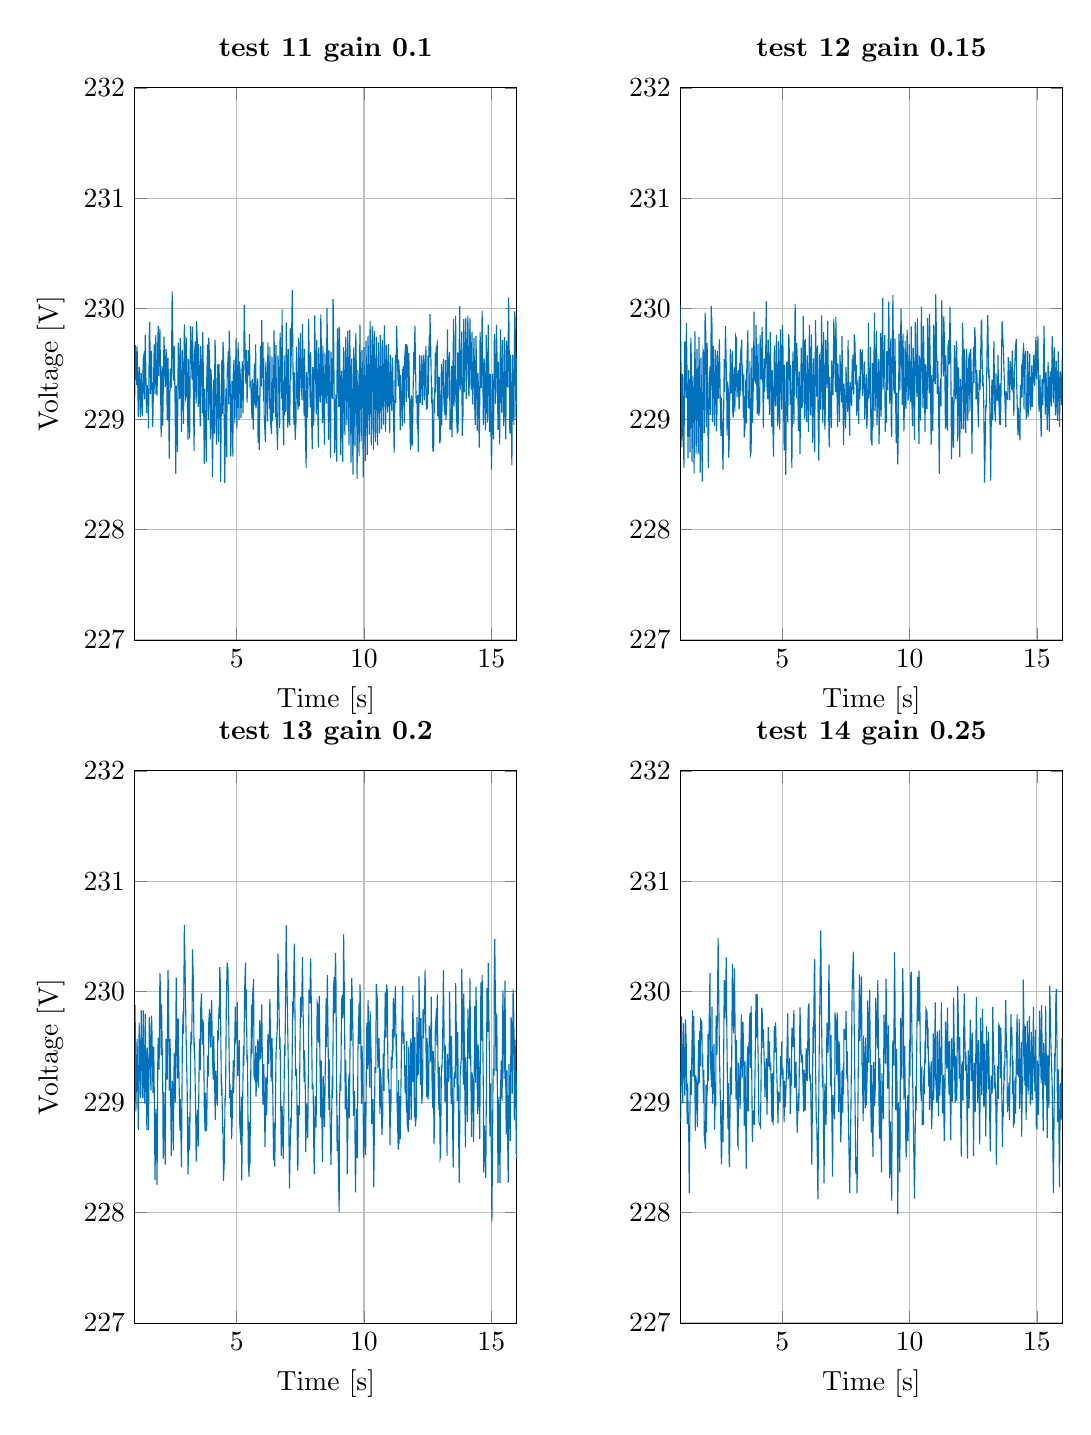
\begin{tikzpicture}

\begin{axis}[%
width=0.4\textwidth,
height=2.761in,
at={(1.272in,4.208in)},
scale only axis,
xmin=1,
xmax=16,
xlabel={Time [s]},
xmajorgrids,
ymin=227,
ymax=232,
ylabel={Voltage [V]},
ymajorgrids,
axis background/.style={fill=white},
title style={font=\bfseries},
title={test 11 gain 0.1}
]
\addplot [color=mycolor1,solid,forget plot]
  table[row sep=crcr]{%
0.992	229.191800893141\\
1.024	229.670033458846\\
1.072	229.311710836432\\
1.088	229.657800327116\\
1.136	229.021174393387\\
1.168	229.470404169425\\
1.184	229.439255394141\\
1.216	229.018279405422\\
1.232	229.125159168785\\
1.248	229.417739321164\\
1.296	229.02948048983\\
1.328	229.548695550966\\
1.344	229.568325821028\\
1.376	229.178568474376\\
1.408	229.760862569136\\
1.424	229.545430436366\\
1.456	229.05650854431\\
1.488	229.308181544482\\
1.52	229.146710584636\\
1.536	228.917233613161\\
1.568	229.779322018806\\
1.584	229.880590212191\\
1.616	229.226154990788\\
1.648	229.618441950518\\
1.664	229.441471677304\\
1.696	228.931450205781\\
1.712	229.044639731034\\
1.76	229.676234334292\\
1.792	229.224722399243\\
1.824	229.763486201209\\
1.856	229.246090345251\\
1.872	229.214601451993\\
1.904	229.746605172566\\
1.92	229.843080806431\\
1.936	229.391542614274\\
1.984	229.820123146154\\
2	229.542889378128\\
2.032	228.835968068214\\
2.064	229.482003302846\\
2.096	228.942772362656\\
2.144	229.747206277405\\
2.192	229.290431230126\\
2.224	229.633469822503\\
2.24	229.578432700532\\
2.272	228.988944728311\\
2.304	229.554469323711\\
2.336	228.925852471983\\
2.352	228.64358645854\\
2.384	229.387090202711\\
2.4	229.458430239038\\
2.432	229.285301557769\\
2.464	230.15718221907\\
2.48	229.882565069513\\
2.512	229.348444975584\\
2.544	229.663713858872\\
2.576	229.211639928678\\
2.608	228.506210212968\\
2.624	229.302718569181\\
2.672	228.701173788586\\
2.704	229.692430259727\\
2.72	229.605333099684\\
2.752	229.182155385056\\
2.768	229.258531512928\\
2.784	229.733602038187\\
2.832	228.885199996047\\
2.864	229.628586620077\\
2.912	228.955017452756\\
2.944	229.857712075386\\
2.976	229.616218170363\\
2.992	229.189875252044\\
3.008	229.206991414886\\
3.024	229.73649678234\\
3.088	228.813914005426\\
3.104	229.543411317571\\
3.152	228.825944083303\\
3.184	229.842229105922\\
3.2	229.739020341844\\
3.248	229.357700776877\\
3.264	229.837177445636\\
3.296	229.262445116381\\
3.328	228.709881731543\\
3.344	229.595989121382\\
3.376	229.70466955918\\
3.392	229.259877890821\\
3.408	229.140255766551\\
3.424	229.890031516869\\
3.456	229.686580597144\\
3.488	229.108311323309\\
3.504	229.680814825971\\
3.568	228.934881000504\\
3.584	229.6627709237\\
3.632	229.326282249711\\
3.648	229.051956947258\\
3.664	229.788079979087\\
3.68	229.596723631499\\
3.728	228.595433629806\\
3.744	229.274340185096\\
3.808	228.611388978254\\
3.824	229.367182531356\\
3.856	229.677814191978\\
3.888	228.99174743519\\
3.904	229.737789885984\\
3.936	229.514591807192\\
3.968	228.817273420216\\
3.984	229.45662461583\\
4.016	229.342109228337\\
4.048	228.478309688899\\
4.096	229.357078624612\\
4.112	229.148984350912\\
4.128	228.868475578741\\
4.144	229.719361094112\\
4.16	229.650043113229\\
4.208	228.769144987346\\
4.256	229.495771242948\\
4.288	228.79345409744\\
4.304	229.500270985666\\
4.352	229.006556195272\\
4.368	228.431440940234\\
4.4	229.267483351244\\
4.416	229.540275962083\\
4.448	229.04753003982\\
4.464	229.69996466061\\
4.496	229.45816683392\\
4.528	228.421880735853\\
4.56	228.955110656838\\
4.576	229.278652628898\\
4.608	228.655366115274\\
4.624	229.399409953705\\
4.672	229.615132348338\\
4.688	229.133148042032\\
4.704	229.803954580801\\
4.736	229.558457476087\\
4.768	228.663254322853\\
4.816	229.345000453155\\
4.832	229.096802833511\\
4.848	228.662043261737\\
4.864	229.401623497843\\
4.896	229.536875244344\\
4.928	228.962370872001\\
4.976	229.738714444081\\
5.008	228.915642335785\\
5.056	229.695337500224\\
5.072	229.317534905568\\
5.088	228.992587305029\\
5.104	229.52274800572\\
5.136	229.426532063355\\
5.168	229.012426395848\\
5.216	229.523737513377\\
5.248	229.053772890803\\
5.28	229.505815254398\\
5.296	230.032427980936\\
5.312	229.811890557136\\
5.36	229.321788171955\\
5.376	229.626324309611\\
5.408	229.149255238824\\
5.456	229.625105819762\\
5.488	229.39756425962\\
5.504	229.769728287047\\
5.52	229.310249945858\\
5.552	229.331162806971\\
5.6	229.004930385806\\
5.616	229.362809686967\\
5.648	228.906225650587\\
5.696	229.504008424679\\
5.728	229.124637338185\\
5.744	229.677148767259\\
5.76	229.098465989492\\
5.824	229.369500048079\\
5.84	228.78493347299\\
5.856	229.213529017401\\
5.888	228.719473783596\\
5.936	229.6606335828\\
5.968	229.296528163934\\
5.984	229.896972850776\\
6	229.372980531963\\
6.032	229.696605640925\\
6.048	229.16186268055\\
6.064	229.552778375334\\
6.08	229.030706144469\\
6.128	228.791775734235\\
6.144	229.517900937381\\
6.176	229.314498811421\\
6.208	228.978147235166\\
6.224	229.695679316308\\
6.288	229.096490140233\\
6.304	229.653305350537\\
6.32	229.008236664947\\
6.368	228.866200365881\\
6.384	229.567175367408\\
6.4	228.982384312281\\
6.432	229.368598358819\\
6.448	229.056940505848\\
6.464	229.804003078092\\
6.528	229.017882696935\\
6.544	229.670149308926\\
6.56	229.02916221807\\
6.608	228.718895766397\\
6.624	229.574676463575\\
6.672	229.261119068508\\
6.688	228.918136881515\\
6.704	229.784819457788\\
6.768	229.185306454023\\
6.784	229.994080442485\\
6.8	229.175771065479\\
6.848	228.76334619521\\
6.864	229.576825833171\\
6.88	229.035655201025\\
6.912	229.386219182984\\
6.928	229.066459421468\\
6.944	229.876519750083\\
7.008	228.920577840171\\
7.024	229.634526177176\\
7.04	229.019298234308\\
7.088	228.941824236265\\
7.104	229.823336975554\\
7.12	229.353322558654\\
7.152	229.696864024695\\
7.184	230.168041812437\\
7.216	229.332376237734\\
7.248	228.951045171515\\
7.264	229.424294494346\\
7.296	228.810507827955\\
7.328	228.973584868543\\
7.344	229.657026651234\\
7.36	229.354550419012\\
7.408	229.0872368182\\
7.424	229.736177328856\\
7.456	229.116942114803\\
7.504	229.781799449438\\
7.536	229.287803713555\\
7.568	229.169817265189\\
7.584	229.859753817906\\
7.6	229.580483490059\\
7.648	229.028341513555\\
7.664	229.636066103039\\
7.696	228.893648008939\\
7.728	228.559110008264\\
7.744	229.426308620862\\
7.776	229.013932295314\\
7.792	229.121843894118\\
7.824	229.906407493916\\
7.84	229.674617323999\\
7.888	229.107417309274\\
7.904	229.607651965197\\
7.936	229.078080565325\\
7.968	228.728064477672\\
7.984	229.470391262546\\
8.016	228.941480110162\\
8.032	229.009184109166\\
8.064	229.94086257001\\
8.08	229.666833305122\\
8.128	229.040488999145\\
8.144	229.718465609011\\
8.208	228.745526670904\\
8.224	229.6480620676\\
8.272	229.210628937009\\
8.288	229.149201725637\\
8.304	229.948673068628\\
8.32	229.720831791551\\
8.368	228.96510275509\\
8.384	229.663979055102\\
8.448	228.769605528026\\
8.464	229.602371826556\\
8.512	229.175694809186\\
8.528	229.140735042175\\
8.544	230.008071593243\\
8.56	229.776500860014\\
8.608	228.813546691828\\
8.624	229.622161828742\\
8.688	228.65109817995\\
8.704	229.610990319853\\
8.752	229.209711670334\\
8.768	229.183218506334\\
8.784	230.087080834804\\
8.8	229.948862629132\\
8.848	228.689884134662\\
8.896	229.224938799085\\
8.928	228.615704366518\\
8.944	229.592029771372\\
8.96	229.82107479662\\
8.992	229.382271474738\\
9.008	229.110241679189\\
9.024	229.834881590719\\
9.04	229.80305074793\\
9.088	228.674408671391\\
9.12	229.43641328094\\
9.168	228.610686746311\\
9.184	229.425102757969\\
9.2	229.65188369406\\
9.232	229.124993382946\\
9.248	228.855086683914\\
9.28	229.744250093984\\
9.328	228.947643605865\\
9.36	229.800249484304\\
9.376	229.618820537036\\
9.408	228.7614208704\\
9.44	229.808173494171\\
9.472	229.227747130739\\
9.488	228.606745628895\\
9.52	229.547857782417\\
9.568	228.498360653971\\
9.6	229.649196984636\\
9.648	228.755053176069\\
9.664	229.523926481752\\
9.68	229.781109148147\\
9.712	229.182654335381\\
9.728	228.458908487422\\
9.76	229.44390053043\\
9.808	228.6651462243\\
9.84	229.855678462227\\
9.856	229.477959528638\\
9.888	228.800150129741\\
9.92	229.627526802568\\
9.952	229.246469285472\\
9.968	228.472786549515\\
10	229.652949560347\\
10.048	228.621020351386\\
10.08	229.71030059866\\
10.128	228.676179351278\\
10.144	229.36287276636\\
10.16	229.757671362558\\
10.208	228.859634178962\\
10.24	229.890620633662\\
10.288	228.759975636237\\
10.32	229.84481865893\\
10.352	229.59523026425\\
10.368	228.724468375562\\
10.384	229.301605566199\\
10.4	229.801496992562\\
10.448	228.794655412927\\
10.48	229.747903885548\\
10.528	228.763184331294\\
10.56	229.696213006238\\
10.576	229.510199004072\\
10.608	228.871921482627\\
10.624	229.254630572512\\
10.64	229.761882390986\\
10.688	228.908624098582\\
10.72	229.718793819485\\
10.768	228.950445542635\\
10.8	229.849552507557\\
10.816	229.664665032042\\
10.848	228.887773842525\\
10.864	229.156412023076\\
10.88	229.671707085066\\
10.928	229.06274060566\\
10.96	229.680293556933\\
11.008	228.872909520263\\
11.04	229.581150498247\\
11.088	229.076608578364\\
11.12	229.558056062353\\
11.136	229.363437219224\\
11.184	228.69776920829\\
11.232	229.57908143752\\
11.248	229.147959957233\\
11.28	229.848053062636\\
11.328	229.429623900369\\
11.344	229.297718327589\\
11.36	229.539338196473\\
11.392	229.407949042749\\
11.424	228.898392073067\\
11.44	229.398604124087\\
11.504	228.939210912732\\
11.52	229.439746945885\\
11.552	229.482614188527\\
11.568	229.160928456596\\
11.584	228.961500789222\\
11.6	229.557824491238\\
11.632	229.679722564033\\
11.664	229.157096633842\\
11.68	229.677127938437\\
11.712	229.632178564575\\
11.744	229.193996220098\\
11.76	229.597603691567\\
11.808	228.921348025189\\
11.824	228.723496942051\\
11.84	229.152825200863\\
11.872	229.214178068676\\
11.888	228.756095808861\\
11.904	228.808090935898\\
11.952	229.608691711713\\
11.968	229.402936309508\\
12	229.847172515291\\
12.048	229.145414902606\\
12.08	229.206234055768\\
12.096	228.91146692504\\
12.112	229.219705343468\\
12.128	228.701155880547\\
12.144	228.977962297538\\
12.192	229.581975590921\\
12.208	229.14444999496\\
12.272	229.578670346054\\
12.288	229.127810770178\\
12.32	229.455980794203\\
12.352	229.586814521331\\
12.368	229.17114265088\\
12.384	229.276226420996\\
12.432	229.663125982927\\
12.448	229.091804591098\\
12.496	229.10314836411\\
12.512	229.574447660682\\
12.528	229.221792778139\\
12.56	229.744552279399\\
12.576	229.559338603825\\
12.592	229.95057559584\\
12.624	229.62188883506\\
12.656	229.144287660712\\
12.672	229.289796754823\\
12.704	228.711165299758\\
12.736	228.713238728177\\
12.752	229.195472838778\\
12.768	229.055727690749\\
12.8	229.602349681016\\
12.816	229.243478771489\\
12.832	229.630884297402\\
12.88	229.684323999998\\
12.896	229.025991025869\\
12.912	229.387462235984\\
12.944	229.001024899399\\
12.96	229.37987329452\\
12.976	228.780152307077\\
13.008	228.837547130319\\
13.04	229.50091926514\\
13.056	228.947079813436\\
13.072	229.318293485502\\
13.12	229.545035875772\\
13.136	229.151233513578\\
13.184	229.035041355897\\
13.2	229.53434252381\\
13.216	228.990700708785\\
13.248	229.116343988466\\
13.28	229.813335003031\\
13.296	229.189579038082\\
13.312	229.476437947058\\
13.36	229.608367414983\\
13.376	228.909634611894\\
13.424	228.914830754091\\
13.44	229.481241734103\\
13.456	228.835181364439\\
13.52	229.908892878853\\
13.536	229.116438326675\\
13.584	229.420246963415\\
13.6	229.936139511024\\
13.616	229.127891225506\\
13.664	228.869020333089\\
13.68	229.605629083912\\
13.696	228.88829707005\\
13.76	230.023649913715\\
13.776	229.262953477539\\
13.808	229.391103603282\\
13.84	229.793400917377\\
13.856	228.847952253558\\
13.888	229.032534926239\\
13.92	229.90630099397\\
13.936	229.24268341358\\
14	229.920244282664\\
14.016	229.182192858824\\
14.032	229.368399878381\\
14.08	229.938786836778\\
14.112	229.233754540779\\
14.128	229.206495374407\\
14.16	229.913999913438\\
14.208	229.268597813529\\
14.24	229.789998996746\\
14.256	229.326005180837\\
14.272	229.134621238541\\
14.32	229.733178755388\\
14.352	229.088540739385\\
14.368	228.948508654546\\
14.4	229.754565589928\\
14.448	228.897003416679\\
14.48	229.417132320261\\
14.528	228.743224163159\\
14.544	229.108890926599\\
14.56	229.789087059444\\
14.608	229.278833316078\\
14.64	229.982742651426\\
14.688	228.945716434958\\
14.72	229.550433238193\\
14.736	229.37678337048\\
14.768	228.899492880377\\
14.784	229.10414453868\\
14.8	229.760122284595\\
14.848	228.96979362247\\
14.88	229.855761558323\\
14.928	228.884743293811\\
14.96	229.407558024545\\
14.976	229.074840065964\\
15.008	228.542959544791\\
15.024	228.806099071548\\
15.04	229.412448564393\\
15.088	228.81623963527\\
15.12	229.770487447524\\
15.168	229.136918037953\\
15.2	229.855773470625\\
15.216	229.698999052481\\
15.264	228.904364440545\\
15.28	229.520595072471\\
15.328	228.772324100265\\
15.36	229.81291533545\\
15.408	229.060128780725\\
15.44	229.714693253278\\
15.456	229.451058556047\\
15.488	228.937102189546\\
15.504	229.089976245235\\
15.52	229.742917914901\\
15.568	228.816719180483\\
15.6	229.708821694709\\
15.648	229.286287781446\\
15.68	230.103685241094\\
15.696	229.832670977708\\
15.728	228.868909312139\\
15.744	228.904217678549\\
15.76	229.581403388564\\
15.808	228.582376699034\\
15.84	229.583705825749\\
15.888	228.946955924563\\
15.92	229.975961850116\\
15.936	229.885967773054\\
15.968	229.015810571393\\
16.016	229.611362565593\\
};
\end{axis}

\begin{axis}[%
width=0.4\textwidth,
height=2.761in,
at={(4in,4.208in)},
scale only axis,
xmin=1,
xmax=16,
xlabel={Time [s]},
xmajorgrids,
ymin=227,
ymax=232,
ymajorgrids,
axis background/.style={fill=white},
title style={font=\bfseries},
title={test 12  gain 0.15}
]
\addplot [color=mycolor1,solid,forget plot]
  table[row sep=crcr]{%
0.992	230.036113863287\\
1.04	229.115032809442\\
1.056	228.744738036754\\
1.072	229.406766212873\\
1.088	229.378712586497\\
1.136	228.557543008092\\
1.168	229.70284278669\\
1.216	229.191862768011\\
1.232	229.87087193445\\
1.28	229.067602380819\\
1.296	228.644553944122\\
1.328	229.445780718374\\
1.376	228.700012422668\\
1.408	229.739572573369\\
1.424	229.57196292983\\
1.456	228.610922562889\\
1.488	229.395419517651\\
1.52	229.126289137252\\
1.536	228.508824540578\\
1.568	229.797797238747\\
1.616	228.688961188786\\
1.648	229.634567820959\\
1.664	229.331744771916\\
1.696	228.685568424478\\
1.712	229.170148450512\\
1.728	229.743263668459\\
1.776	228.516334002796\\
1.808	229.556308562203\\
1.856	228.436860560971\\
1.888	229.624948397021\\
1.92	229.591612984727\\
1.936	228.873181575997\\
1.952	229.404825017507\\
1.968	229.964351717255\\
2	229.747605062802\\
2.016	228.927565028844\\
2.048	229.688922670182\\
2.096	228.557193050054\\
2.128	229.304308353718\\
2.16	229.47772549606\\
2.176	229.039032392572\\
2.192	229.401642760044\\
2.208	230.025470002028\\
2.24	229.849771383349\\
2.256	228.97296569342\\
2.288	229.663465202472\\
2.336	228.937449610965\\
2.368	229.630470829404\\
2.384	229.487204734942\\
2.416	228.890713241021\\
2.432	228.999146002397\\
2.448	229.617778979582\\
2.496	229.186437244978\\
2.528	229.72348181877\\
2.576	228.975548395698\\
2.592	228.849628916634\\
2.608	229.195946829681\\
2.624	229.053931289333\\
2.672	228.542426449571\\
2.72	229.544259356785\\
2.736	229.247834729516\\
2.768	229.845459344511\\
2.816	229.285546503113\\
2.832	228.850905716554\\
2.848	229.339862761245\\
2.88	229.263504880942\\
2.896	228.651757594766\\
2.912	228.769120700595\\
2.96	229.635244392092\\
2.992	229.232626849282\\
3.04	229.618102534691\\
3.056	229.056164064632\\
3.072	229.015479250862\\
3.088	229.33542211206\\
3.12	229.469097039374\\
3.136	229.068174545456\\
3.152	229.286633454441\\
3.168	229.754440214101\\
3.2	229.726743988066\\
3.216	229.196919582027\\
3.28	229.443330127369\\
3.296	229.101389623945\\
3.312	229.098262588655\\
3.328	229.505948025685\\
3.344	229.208243674525\\
3.36	229.580650348282\\
3.408	229.719234707152\\
3.424	229.252538655189\\
3.44	229.489539285909\\
3.472	229.011433699789\\
3.488	229.402857242768\\
3.504	228.836512185025\\
3.536	228.924873139052\\
3.568	229.366738278967\\
3.584	228.962377661344\\
3.6	229.409738782721\\
3.648	229.80609670027\\
3.664	229.108605097085\\
3.712	229.10067092785\\
3.728	229.524909441049\\
3.744	228.672543243947\\
3.776	228.703948962233\\
3.808	229.646881875648\\
3.824	228.965793576417\\
3.872	229.377995735716\\
3.888	229.973892707501\\
3.904	229.37067485236\\
3.952	229.336160434686\\
3.968	229.852781597001\\
4.016	229.04866018981\\
4.048	229.679341367228\\
4.064	229.165343128017\\
4.08	229.030323261503\\
4.112	229.104250875243\\
4.128	229.761142290154\\
4.176	229.357486456021\\
4.208	229.8362862728\\
4.256	228.923336466278\\
4.288	229.5481075594\\
4.304	229.250766329699\\
4.352	229.670033527781\\
4.368	230.067700419714\\
4.4	229.291629381438\\
4.432	229.17902759226\\
4.448	229.719721024869\\
4.496	229.040178077535\\
4.528	229.788783910937\\
4.544	229.531497592899\\
4.576	228.932209586401\\
4.608	229.445254784923\\
4.64	228.800592356304\\
4.656	228.661669776231\\
4.688	229.667423634397\\
4.736	229.115498034743\\
4.768	229.762856315247\\
4.784	229.430253929799\\
4.816	228.935415362192\\
4.832	229.040191225952\\
4.848	229.703710752432\\
4.896	228.906546585759\\
4.928	229.814093428997\\
4.976	229.08808041471\\
5.008	229.852457564791\\
5.024	229.686817366129\\
5.072	228.716720048047\\
5.088	229.491966721294\\
5.136	228.495142571539\\
5.168	229.494208661396\\
5.184	229.523288918132\\
5.216	228.975633783391\\
5.248	229.767098524471\\
5.264	229.732914787173\\
5.312	229.131439668691\\
5.328	229.49055418454\\
5.376	228.559007027414\\
5.408	229.49048335964\\
5.424	229.612916234332\\
5.456	228.95860570984\\
5.504	230.044254939326\\
5.552	229.190797279689\\
5.568	229.687536066656\\
5.6	229.46650787735\\
5.632	228.893099079775\\
5.664	229.430191012805\\
5.696	228.686980453717\\
5.744	229.647601876671\\
5.776	229.099159453402\\
5.792	229.15303218823\\
5.824	229.936465837068\\
5.872	229.005709477664\\
5.888	229.706414146021\\
5.904	229.711854978209\\
5.936	229.073046050948\\
5.952	228.97550295278\\
5.984	229.576790542343\\
6.016	229.008508606225\\
6.032	228.884439285182\\
6.064	229.851250334186\\
6.112	229.034992214838\\
6.144	229.765384819312\\
6.16	229.372904065041\\
6.192	228.784905620546\\
6.224	229.549757998455\\
6.256	229.044079068115\\
6.272	228.701254614873\\
6.304	229.898077506463\\
6.352	229.203352460448\\
6.384	229.666879953013\\
6.4	229.131895517995\\
6.432	228.625809641321\\
6.448	228.953195714767\\
6.464	229.589064347238\\
6.512	229.087654051613\\
6.544	229.94034480947\\
6.592	228.965431638089\\
6.624	229.788029935637\\
6.64	229.385812075621\\
6.672	228.904500972587\\
6.688	229.075348554623\\
6.704	229.719105683668\\
6.752	229.28241564552\\
6.784	229.889856261696\\
6.832	228.859344414407\\
6.848	228.747863440986\\
6.864	229.383427464655\\
6.88	229.260292037791\\
6.928	228.920908149297\\
6.944	229.529320278651\\
6.992	229.218105620195\\
7.024	229.906247696265\\
7.072	229.401137688051\\
7.088	229.246748603124\\
7.104	229.924998150714\\
7.12	229.687065251209\\
7.168	228.927725826657\\
7.184	229.504498402178\\
7.248	228.973571478278\\
7.264	229.583823791122\\
7.312	229.305549523347\\
7.328	229.153071720605\\
7.344	229.754803014665\\
7.36	229.513686176775\\
7.408	228.764351808432\\
7.424	229.322521444174\\
7.488	228.916453834923\\
7.504	229.47195515156\\
7.52	229.328551059545\\
7.568	229.066856505835\\
7.584	229.715355036346\\
7.6	229.385316010421\\
7.648	228.850760967019\\
7.664	229.334947004807\\
7.728	229.121862260081\\
7.744	229.544856698488\\
7.76	229.265363000794\\
7.776	229.585035820231\\
7.808	229.224413091192\\
7.824	229.766946354634\\
7.856	229.688281035644\\
7.888	229.310360204338\\
7.904	229.492905095202\\
7.92	229.032741919101\\
7.936	229.357104268655\\
7.968	229.194294346791\\
8	228.955075274404\\
8.016	229.38823881596\\
8.048	229.182485888669\\
8.064	229.635810752627\\
8.08	229.268761011335\\
8.096	229.58501818094\\
8.144	229.613167551875\\
8.16	229.211733501473\\
8.208	229.381935727272\\
8.224	229.522396752554\\
8.24	229.003238586424\\
8.304	229.404540025233\\
8.32	228.912258573335\\
8.368	229.258732514441\\
8.384	229.869666446627\\
8.4	229.186439327192\\
8.448	229.351838176166\\
8.464	229.654611084729\\
8.48	228.822387240836\\
8.528	228.762262387965\\
8.544	229.507891964292\\
8.56	228.926123460568\\
8.592	229.416331831264\\
8.624	229.964076314137\\
8.64	229.075607057678\\
8.656	229.154725226739\\
8.704	229.800801361082\\
8.72	228.945615271895\\
8.784	229.545766248038\\
8.8	228.774085190709\\
8.832	229.219341043444\\
8.864	229.780297382379\\
8.88	229.024270293721\\
8.896	229.242789707185\\
8.944	230.096496121687\\
8.96	229.270254538571\\
9.024	229.760611648261\\
9.04	228.885191760965\\
9.072	229.095359888162\\
9.088	228.966869684845\\
9.104	229.615059674245\\
9.136	229.262406109475\\
9.184	230.067376748375\\
9.216	229.141127908735\\
9.264	229.732059373165\\
9.28	228.944633885526\\
9.296	228.83810347782\\
9.328	229.736204428271\\
9.344	230.123260536946\\
9.376	229.276218964493\\
9.408	229.231018167559\\
9.424	229.731358465552\\
9.472	228.784188180801\\
9.504	229.239990227641\\
9.52	228.754477509878\\
9.536	228.590695725754\\
9.568	229.0734475204\\
9.584	229.77474317027\\
9.616	229.265595399646\\
9.664	229.997970571277\\
9.712	229.128109688279\\
9.744	229.774843894551\\
9.776	228.889397358657\\
9.808	229.228159362631\\
9.824	229.707326648096\\
9.856	229.093041703273\\
9.904	229.810161835136\\
9.936	229.167598317315\\
9.968	229.226744689098\\
9.984	229.679513866004\\
10	229.429418848762\\
10.048	229.155644191522\\
10.064	229.840252010326\\
10.096	229.099964585832\\
10.112	228.938270972213\\
10.144	229.64895600418\\
10.192	228.812257201342\\
10.224	229.877994849953\\
10.24	229.582704376335\\
10.288	229.202469098343\\
10.304	229.911855416611\\
10.368	228.775263259059\\
10.384	229.576052590948\\
10.432	228.987585015795\\
10.464	230.019309770227\\
10.48	229.757140820577\\
10.528	229.100543126026\\
10.544	229.845080513837\\
10.608	228.884477598955\\
10.624	229.496065258202\\
10.672	229.099038849887\\
10.688	229.096947762073\\
10.704	229.91682858435\\
10.72	229.752771301214\\
10.768	229.235413378009\\
10.784	229.953387253657\\
10.848	228.768171244612\\
10.864	229.401686419451\\
10.912	228.891733329432\\
10.944	229.855499013144\\
10.96	229.726794125259\\
10.992	229.321618031148\\
11.008	229.321702811924\\
11.024	230.130061146406\\
11.04	229.94984985648\\
11.088	229.229357482844\\
11.104	229.526705040243\\
11.136	229.147785888402\\
11.168	228.50477630886\\
11.184	229.242891976468\\
11.216	229.366616369192\\
11.232	229.116172784981\\
11.264	230.076144178636\\
11.28	229.758694048973\\
11.328	229.387284761642\\
11.344	229.933443116854\\
11.376	229.621717998697\\
11.408	228.913509185624\\
11.424	229.577009845816\\
11.472	228.92668661281\\
11.488	228.89648751387\\
11.504	229.64164029008\\
11.536	229.715061144211\\
11.552	229.494896521905\\
11.568	229.542199305397\\
11.584	230.016219304711\\
11.616	229.57935339513\\
11.648	228.636934525256\\
11.68	229.202012541251\\
11.712	228.83288787127\\
11.728	228.7428151513\\
11.76	229.670637734486\\
11.808	229.181023366043\\
11.84	229.708756044087\\
11.856	229.622284160395\\
11.888	228.802355720052\\
11.92	229.469541567602\\
11.952	229.157058822613\\
11.968	228.657107010784\\
12	229.362842223777\\
12.048	228.913315569607\\
12.08	229.874000533759\\
12.112	229.564130813665\\
12.128	228.907312438126\\
12.16	229.638567339063\\
12.176	229.213274174682\\
12.208	228.874027747458\\
12.24	229.636002344347\\
12.288	228.980670963897\\
12.32	229.538042174648\\
12.352	229.603597299812\\
12.368	229.067650439295\\
12.4	229.63689938354\\
12.432	229.293631760988\\
12.448	228.684002406405\\
12.48	229.297745726451\\
12.512	229.655704528438\\
12.528	229.328851670826\\
12.56	229.831195107085\\
12.592	229.667534393403\\
12.608	229.184630464437\\
12.624	229.184755119701\\
12.64	229.447195205396\\
12.704	228.925936348846\\
12.72	229.284647410528\\
12.752	229.445031040334\\
12.768	229.265905848111\\
12.816	229.883609026853\\
12.832	229.891227080974\\
12.864	229.300917292569\\
12.88	229.403947364985\\
12.912	229.160014973269\\
12.944	228.424638336973\\
12.96	228.623327074024\\
12.992	229.112319827418\\
13.008	229.108632055933\\
13.056	229.822298179186\\
13.072	229.942118548927\\
13.104	229.376498699208\\
13.12	229.456449435134\\
13.152	229.13085788298\\
13.184	228.444822790134\\
13.2	228.852858115611\\
13.232	229.35829295199\\
13.264	228.988768594087\\
13.296	229.486918489991\\
13.312	229.708484878144\\
13.344	229.083199679866\\
13.376	228.978203701981\\
13.392	229.415098667574\\
13.408	229.177501541763\\
13.456	229.17335851962\\
13.472	229.58006005166\\
13.488	229.31587899001\\
13.536	228.950114612078\\
13.552	229.323401330747\\
13.568	228.945315639764\\
13.584	229.143060439265\\
13.632	229.888430920136\\
13.68	229.651320053872\\
13.728	229.295245062669\\
13.776	228.92837731409\\
13.792	229.252774143533\\
13.856	229.17461874555\\
13.872	229.560977230959\\
13.92	229.287324831529\\
13.936	229.170293332722\\
13.952	229.528340298288\\
13.968	229.486757963268\\
14.016	229.263228052778\\
14.032	229.621348667097\\
14.096	229.027477709144\\
14.112	229.372595992797\\
14.16	229.665109948046\\
14.192	229.726011654402\\
14.208	229.298253055587\\
14.256	228.852548529775\\
14.272	229.105530257372\\
14.336	228.808073040029\\
14.352	229.30988878331\\
14.384	229.191557351707\\
14.4	229.496314502233\\
14.416	229.200516051094\\
14.448	229.55649186282\\
14.48	229.688801811988\\
14.496	229.089813952096\\
14.512	229.511539465164\\
14.56	229.614950515331\\
14.576	228.998299224388\\
14.624	229.121688155326\\
14.64	229.61694830406\\
14.656	229.017536765311\\
14.72	229.59280226456\\
14.736	229.110607884287\\
14.752	229.097781580892\\
14.768	229.159980162595\\
14.8	229.486116184608\\
14.816	229.111108421654\\
14.832	229.222651294404\\
14.88	229.583989926188\\
14.912	229.298614818261\\
14.96	229.742828287583\\
14.976	229.390124598907\\
14.992	229.361827304667\\
15.024	229.60525808699\\
15.04	229.756390159045\\
15.072	229.139145670127\\
15.088	229.066252320929\\
15.12	229.401221542846\\
15.168	228.838854802719\\
15.2	229.361266530996\\
15.232	229.124411816603\\
15.264	229.537607671535\\
15.28	229.844897127746\\
15.312	229.308950082147\\
15.328	229.041891115397\\
15.36	229.425120795395\\
15.408	228.903948735783\\
15.44	229.517653560842\\
15.456	229.365548667235\\
15.488	228.888135853545\\
15.504	229.177960110468\\
15.52	229.434381491127\\
15.568	229.114189533457\\
15.6	229.752619204441\\
15.648	229.151061209528\\
15.68	229.649745650544\\
15.696	229.513845628246\\
15.728	229.033655127802\\
15.744	229.145633937267\\
15.76	229.529034130006\\
15.808	228.984713510172\\
15.84	229.614303572013\\
15.888	228.929467087073\\
15.92	229.432968354798\\
15.968	229.126104942236\\
15.984	229.385806189006\\
16.016	229.754557017209\\
};
\end{axis}

\begin{axis}[%
width=0.4\textwidth,
height=2.761in,
at={(1.272in,0.793in)},
scale only axis,
xmin=1,
xmax=16,
xlabel={Time [s]},
xmajorgrids,
ymin=227,
ymax=232,
ylabel={Voltage [V]},
ymajorgrids,
axis background/.style={fill=white},
title style={font=\bfseries},
title={test 13  gain 0.2}
]
\addplot [color=mycolor1,solid,forget plot]
  table[row sep=crcr]{%
0.992	229.404971813662\\
1.008	229.879919443127\\
1.04	228.915741051664\\
1.088	229.572114039215\\
1.136	228.74912723183\\
1.168	229.720268123837\\
1.184	229.513431356322\\
1.216	229.039476051979\\
1.232	229.079105103484\\
1.248	229.835715821339\\
1.312	229.036473510289\\
1.328	229.832333863015\\
1.376	229.040481623144\\
1.392	228.987203636536\\
1.408	229.798708770686\\
1.424	229.481954079687\\
1.472	228.748126967642\\
1.488	229.495089837453\\
1.536	228.746070990976\\
1.568	229.771752542874\\
1.616	229.227521514972\\
1.632	229.107258443081\\
1.648	229.783124640106\\
1.664	229.737246444826\\
1.712	229.085246052992\\
1.744	229.500896374943\\
1.76	229.123756848244\\
1.792	228.297574319485\\
1.824	228.93707595756\\
1.856	228.602551967346\\
1.872	228.248854438156\\
1.904	229.472359590711\\
1.92	229.585259585253\\
1.952	229.294020214034\\
1.984	230.168335026885\\
2	230.068061701338\\
2.032	229.426289340203\\
2.048	229.88598934382\\
2.096	229.140174042942\\
2.112	228.485310093007\\
2.144	229.088741054878\\
2.192	228.433580072759\\
2.224	229.570575028921\\
2.272	229.203378349802\\
2.288	229.911094790694\\
2.304	230.197878998509\\
2.336	229.674412387116\\
2.352	229.103909361695\\
2.384	229.572835117683\\
2.432	228.512726452107\\
2.464	229.195430177334\\
2.496	229.141194235351\\
2.512	228.562476088365\\
2.528	229.023370726073\\
2.544	229.449427450697\\
2.592	228.998719656126\\
2.624	230.128903355276\\
2.672	229.214501271375\\
2.704	229.75689938339\\
2.72	229.439997987588\\
2.768	228.742568553954\\
2.784	229.027050360076\\
2.832	228.412057477447\\
2.864	229.523701685923\\
2.896	229.824095861552\\
2.912	229.619219295022\\
2.944	230.606188403232\\
2.96	230.388907656993\\
3.008	229.667063350793\\
3.056	229.086497453963\\
3.088	228.34560991134\\
3.136	228.867325630523\\
3.152	228.565861668789\\
3.2	229.598969250683\\
3.232	229.561975823248\\
3.248	229.824400915065\\
3.264	230.384348239379\\
3.296	230.107090212655\\
3.328	229.443918939208\\
3.344	229.540502341953\\
3.392	228.83930648092\\
3.408	228.460994805229\\
3.456	228.931559806953\\
3.488	228.599667878095\\
3.536	229.57329362442\\
3.568	229.291228546838\\
3.584	229.828544149154\\
3.616	229.985337144039\\
3.632	229.734965957582\\
3.648	229.520604515025\\
3.664	229.749343409413\\
3.696	229.703647245474\\
3.728	228.94154188608\\
3.76	228.732483082772\\
3.776	229.086387212509\\
3.808	228.741409818902\\
3.824	228.799731255024\\
3.856	229.420752206545\\
3.888	229.232753218046\\
3.904	229.727743769966\\
3.936	229.841334414823\\
3.968	229.493855659699\\
4.016	229.92615425425\\
4.048	229.392703695079\\
4.08	229.20342504098\\
4.096	229.598175757407\\
4.128	229.225820496629\\
4.16	228.840117716222\\
4.176	229.283200951841\\
4.24	228.970136280353\\
4.256	229.648788884803\\
4.272	229.55881485332\\
4.304	229.859468771546\\
4.32	229.755989256228\\
4.336	230.223571351565\\
4.352	230.118722050664\\
4.4	229.059039253904\\
4.416	229.178400828997\\
4.448	228.741665389939\\
4.464	228.751153834898\\
4.48	228.286620283023\\
4.512	228.45716694835\\
4.544	229.062656377075\\
4.56	229.007337121929\\
4.592	229.869798956895\\
4.624	230.264550790354\\
4.656	230.207115392927\\
4.688	229.742410011805\\
4.72	229.036270867612\\
4.736	229.1659483815\\
4.768	228.861560062019\\
4.784	229.109656870287\\
4.8	228.66547784081\\
4.832	228.921118340781\\
4.864	229.378441577281\\
4.88	229.085359760498\\
4.928	229.608770344619\\
4.944	229.865178687609\\
4.96	229.561154312486\\
5.008	229.617021079486\\
5.024	229.905020516725\\
5.04	229.23816936719\\
5.104	229.562216667387\\
5.12	228.80304559776\\
5.168	228.615671351747\\
5.184	229.05013064433\\
5.2	228.292152373918\\
5.216	228.698845593824\\
5.264	229.507159991758\\
5.28	229.326790817898\\
5.312	230.012687451291\\
5.344	230.263361544791\\
5.36	229.758988270044\\
5.376	230.021625546588\\
5.408	229.355864754374\\
5.424	229.428366632699\\
5.456	228.435423737822\\
5.488	228.321907290163\\
5.504	228.821146014285\\
5.52	228.44020091284\\
5.552	229.255534183818\\
5.584	229.883814884405\\
5.6	229.440322309957\\
5.632	229.986114190258\\
5.664	230.114915699669\\
5.68	229.237621027173\\
5.728	229.194785927498\\
5.744	229.509098696073\\
5.76	229.050074524403\\
5.824	229.567823553727\\
5.84	229.160303133978\\
5.856	229.149060509985\\
5.888	229.556505240379\\
5.904	229.7415341375\\
5.936	229.386882664378\\
5.984	229.885938027828\\
6.016	229.172279532919\\
6.032	228.976947247046\\
6.064	229.344166868466\\
6.112	228.595404684424\\
6.144	229.228907405324\\
6.176	228.881029920139\\
6.208	229.299080842267\\
6.224	229.614204098007\\
6.256	229.345547524532\\
6.304	229.934367759367\\
6.352	229.185507367496\\
6.384	229.580590082085\\
6.4	229.433959233051\\
6.448	228.473500578588\\
6.464	228.813979241378\\
6.496	228.417019414525\\
6.544	229.447934490708\\
6.592	229.665447629013\\
6.624	230.34556444848\\
6.64	230.181277658339\\
6.688	229.478505301492\\
6.704	229.586104946129\\
6.736	228.82651730912\\
6.752	228.515059573221\\
6.784	228.963628807019\\
6.832	228.487337667237\\
6.88	229.523634982857\\
6.896	229.419171389188\\
6.928	230.168655797696\\
6.944	230.601069197173\\
6.976	230.059850535617\\
7.024	229.370050863079\\
7.072	228.218641708625\\
7.12	228.853789745583\\
7.136	228.764057721092\\
7.168	229.151337693056\\
7.2	229.914433108879\\
7.216	229.768115984315\\
7.264	230.435517441104\\
7.312	229.236538723695\\
7.344	229.301180759848\\
7.36	229.130247602406\\
7.392	228.380860527543\\
7.408	228.443439757617\\
7.424	228.969835360444\\
7.456	228.880675319705\\
7.504	229.88407384501\\
7.52	229.955270827241\\
7.536	229.769258482963\\
7.552	229.884392431502\\
7.584	230.313648789489\\
7.6	229.982324270424\\
7.648	229.18134919732\\
7.664	229.46847786957\\
7.696	229.100828894041\\
7.712	228.548991963881\\
7.744	228.98827653504\\
7.792	228.676747197038\\
7.84	230.018753357925\\
7.872	229.894327184387\\
7.904	230.302517340177\\
7.936	229.799887460227\\
7.968	229.115657589448\\
8	229.156452203771\\
8.032	228.513241933502\\
8.048	228.349676478322\\
8.08	229.027944403707\\
8.096	229.053646656302\\
8.112	228.768940196832\\
8.128	228.945490501583\\
8.16	229.901213088012\\
8.176	229.885223111213\\
8.208	229.538316462618\\
8.24	229.963583043182\\
8.272	229.348748668086\\
8.304	228.860184069268\\
8.32	229.377368064142\\
8.368	228.456226884755\\
8.4	229.239147225323\\
8.448	228.776455372971\\
8.464	229.020788188431\\
8.512	229.940713527714\\
8.528	229.499710354358\\
8.56	230.150810651711\\
8.608	229.202220219957\\
8.624	228.929998070812\\
8.64	229.388534567926\\
8.656	228.982657193992\\
8.704	228.431797827844\\
8.752	229.227729734522\\
8.768	229.034473606086\\
8.8	230.032300993866\\
8.832	230.131331530154\\
8.848	229.801918402408\\
8.88	230.348932844831\\
8.896	230.171336682047\\
8.944	228.558869217055\\
8.96	228.881376393283\\
9.024	228.002908213296\\
9.04	229.012383726946\\
9.072	229.265199762559\\
9.088	229.102646718395\\
9.12	229.920973896638\\
9.152	229.97296335986\\
9.168	229.756408098592\\
9.184	229.891993669449\\
9.2	230.519215895497\\
9.232	229.900882226747\\
9.264	228.933836009024\\
9.28	229.38495280981\\
9.328	228.821157527765\\
9.344	228.348432911507\\
9.376	228.995730690299\\
9.408	229.25026199866\\
9.424	228.854404282671\\
9.472	229.934135784896\\
9.504	229.557963974034\\
9.52	230.122682024679\\
9.568	229.601166220209\\
9.584	228.876520764887\\
9.632	229.100865090035\\
9.664	228.182699562683\\
9.712	228.941978771715\\
9.744	228.494409321626\\
9.76	229.445991844916\\
9.808	229.899461207463\\
9.824	229.528641126544\\
9.84	230.066240195377\\
9.856	229.968116935083\\
9.904	228.985851407481\\
9.92	229.509499342552\\
9.952	229.331260549916\\
9.984	228.492686434792\\
10.016	228.739191378988\\
10.032	229.004665440344\\
10.064	228.523705952018\\
10.096	229.42967243823\\
10.112	229.720354372477\\
10.144	229.296459834019\\
10.16	229.925578098603\\
10.224	229.132556489017\\
10.24	229.827522111928\\
10.288	229.342667933746\\
10.304	228.802877918435\\
10.352	229.026514805201\\
10.384	228.23037841899\\
10.432	229.31939996382\\
10.464	229.26628463561\\
10.48	230.071243600317\\
10.528	229.910630254595\\
10.544	229.305237448283\\
10.592	229.583243034624\\
10.624	228.895234016612\\
10.64	229.304019378575\\
10.672	229.212700285009\\
10.704	228.702055709751\\
10.736	228.878276856257\\
10.752	229.440756273546\\
10.784	229.102869830687\\
10.8	229.650149668819\\
10.816	229.570212224794\\
10.832	229.994520427842\\
10.864	229.586345263024\\
10.88	230.066931520466\\
10.912	230.016494520175\\
10.944	229.206833825856\\
10.96	229.299469978562\\
11.008	228.865804061759\\
11.024	228.608506701391\\
11.04	229.114210417615\\
11.056	228.910931172626\\
11.072	229.412622804618\\
11.104	229.306794395093\\
11.12	229.658687372216\\
11.136	229.440147343242\\
11.152	229.941797525558\\
11.184	229.585059175436\\
11.232	230.051039155931\\
11.264	229.40879672109\\
11.28	229.616087639697\\
11.296	229.017117206395\\
11.344	228.569690612426\\
11.36	229.202729558475\\
11.376	228.619559502713\\
11.408	229.054121761637\\
11.424	228.666423424946\\
11.472	229.498648709591\\
11.52	230.054106252006\\
11.536	229.529646658585\\
11.568	229.636219175983\\
11.616	229.079667046001\\
11.648	229.336626618935\\
11.664	228.904559570764\\
11.68	229.553579951939\\
11.696	228.805974858242\\
11.744	228.728608303009\\
11.76	229.504624603125\\
11.776	228.839332557556\\
11.84	229.58030301146\\
11.856	228.841796725341\\
11.888	229.541772085654\\
11.904	229.184983558811\\
11.92	229.968641275265\\
11.984	228.865687809034\\
12	229.59029779149\\
12.016	228.779838102015\\
12.064	228.892903346772\\
12.08	229.771964370337\\
12.096	229.238083883332\\
12.128	229.637633560414\\
12.144	229.248739016277\\
12.16	230.140055677512\\
12.224	229.154136366258\\
12.24	229.76150559948\\
12.272	228.985372712983\\
12.304	229.14202593171\\
12.32	229.843637516019\\
12.336	229.577176313697\\
12.368	229.818862592728\\
12.4	230.195487786701\\
12.432	229.52653006585\\
12.464	229.047886181437\\
12.48	229.581364521133\\
12.512	229.025596595973\\
12.544	229.109140818217\\
12.56	229.691421837223\\
12.608	229.577462108344\\
12.624	229.367269786764\\
12.64	229.954986972028\\
12.672	229.200064082272\\
12.704	228.943282366603\\
12.72	229.462804075346\\
12.752	228.617412201995\\
12.768	228.798168547799\\
12.8	229.649767661957\\
12.848	229.850835249964\\
12.864	229.516532298849\\
12.88	229.976185837783\\
12.912	229.17855622273\\
12.944	228.930630045748\\
12.96	229.316706418935\\
12.992	228.492373440335\\
13.008	228.510122192831\\
13.04	229.334100325701\\
13.056	229.275351876396\\
13.088	229.51839819917\\
13.12	230.195949922256\\
13.152	229.472084994211\\
13.184	229.002507381388\\
13.2	229.512385549641\\
13.248	228.75350482263\\
13.264	228.514614256027\\
13.28	229.436477549893\\
13.296	229.340057390328\\
13.312	229.184936286954\\
13.344	229.230113448259\\
13.36	230.001654250833\\
13.424	228.98310231973\\
13.44	229.599859434757\\
13.488	228.65966883305\\
13.504	228.410431694959\\
13.536	229.232950819213\\
13.552	229.13636375848\\
13.568	229.274360490131\\
13.584	229.216234410639\\
13.6	230.079862469318\\
13.664	229.011854309572\\
13.68	229.635251117915\\
13.728	228.477030687335\\
13.744	228.268327110071\\
13.776	229.242721222535\\
13.824	229.402618490811\\
13.84	230.207574686713\\
13.904	229.158616263985\\
13.92	229.98191868714\\
13.968	228.913479313601\\
13.984	228.591422612201\\
14	229.405240024464\\
14.016	229.258694208638\\
14.064	228.820681728887\\
14.08	229.84965067475\\
14.144	229.393100100809\\
14.16	230.123848556114\\
14.208	229.027788714264\\
14.224	228.686272783921\\
14.24	229.269851761497\\
14.272	229.202225493159\\
14.304	228.640108857277\\
14.352	229.868821186798\\
14.384	229.177585095812\\
14.4	230.047163219291\\
14.448	229.155463558331\\
14.464	228.894498042104\\
14.48	229.522129423326\\
14.496	229.465527770356\\
14.544	228.666815976291\\
14.592	230.084632960448\\
14.624	229.557090193397\\
14.64	230.152320310753\\
14.688	229.099672365988\\
14.704	228.363620166675\\
14.736	228.788426860432\\
14.784	228.315326865739\\
14.832	230.032524023135\\
14.864	229.636721877865\\
14.88	230.259032146712\\
14.928	229.352236413605\\
14.944	228.690126794514\\
14.976	229.171379377947\\
15.024	227.919152586845\\
15.072	229.304979305056\\
15.104	229.240171573504\\
15.12	230.28949621911\\
15.136	230.476003845583\\
15.168	229.772123296088\\
15.184	229.282023040253\\
15.2	229.790159237507\\
15.216	229.781587112134\\
15.264	228.269303121778\\
15.296	229.050180285027\\
15.344	228.268941104787\\
15.36	229.083193912553\\
15.392	229.377006869527\\
15.424	229.010943008009\\
15.456	230.011954449013\\
15.504	229.211366178439\\
15.536	230.101710802857\\
15.552	229.682896200389\\
15.584	228.706496599423\\
15.616	229.288347274908\\
15.632	228.861692145768\\
15.664	228.270923152079\\
15.696	229.34581987508\\
15.744	228.649927353934\\
15.776	229.772509983268\\
15.808	229.677703614106\\
15.824	229.077875053386\\
15.84	229.590865093349\\
15.856	230.022255220729\\
15.888	229.750640859759\\
15.904	228.835386570119\\
15.936	229.565723929085\\
15.984	228.486491024907\\
16.016	229.285244006048\\
};
\end{axis}

\begin{axis}[%
width=0.4\textwidth,
height=2.761in,
at={(4in,0.793in)},
scale only axis,
xmin=1,
xmax=16,
xlabel={Time [s]},
xmajorgrids,
ymin=227,
ymax=232,
ymajorgrids,
axis background/.style={fill=white},
title style={font=\bfseries},
title={test 14  gain 0.25}
]
\addplot [color=mycolor1,solid,forget plot]
  table[row sep=crcr]{%
0.992	229.179150990558\\
1.008	228.819888400829\\
1.04	229.776991826162\\
1.088	228.991983412838\\
1.12	229.713778400732\\
1.152	229.30810901794\\
1.168	229.060193364006\\
1.184	229.152369992222\\
1.2	229.750322893975\\
1.232	229.468451223787\\
1.264	228.800328314682\\
1.28	229.168813892848\\
1.328	228.637619559913\\
1.344	228.177381350521\\
1.376	228.975929797138\\
1.392	229.290902003366\\
1.424	229.064786851367\\
1.472	229.830761306529\\
1.504	229.231026623065\\
1.52	229.7791640976\\
1.568	229.119986163473\\
1.584	228.741088483846\\
1.6	229.242614096456\\
1.632	229.169908547527\\
1.664	228.776662511914\\
1.712	229.564425034641\\
1.744	229.172457680456\\
1.76	229.645507550267\\
1.776	229.327895407823\\
1.792	229.748884334078\\
1.84	229.724514451359\\
1.856	229.316319998099\\
1.872	229.446341293086\\
1.904	228.992292906165\\
1.92	229.293107206798\\
1.936	228.694804541751\\
1.984	228.574918901963\\
2	229.157518020385\\
2.016	228.726994374481\\
2.048	229.163513976352\\
2.064	229.100138347205\\
2.08	229.615424981203\\
2.096	229.192159473747\\
2.128	229.725624655836\\
2.16	230.169279824359\\
2.176	229.376370717018\\
2.224	229.136882144597\\
2.24	229.860926990566\\
2.256	228.986111867861\\
2.32	229.524857118688\\
2.336	228.752417159852\\
2.368	229.051907264827\\
2.384	228.964598859502\\
2.4	229.782845647693\\
2.432	229.427124319408\\
2.48	230.485155633253\\
2.528	229.464254248313\\
2.576	228.942312171463\\
2.608	228.437835997725\\
2.624	228.542650521625\\
2.64	229.019845440056\\
2.672	228.637631384581\\
2.72	230.107830017826\\
2.752	229.761781740255\\
2.8	230.310253246093\\
2.816	229.780834485354\\
2.864	228.75950929745\\
2.88	229.171629432322\\
2.912	228.45304722839\\
2.928	228.414694221076\\
2.96	229.315543958386\\
2.992	229.062904508082\\
3.008	229.239385755854\\
3.04	230.249818288987\\
3.056	230.010459787299\\
3.088	229.623083136292\\
3.12	230.211119138291\\
3.152	229.562670554182\\
3.184	229.024335030524\\
3.2	229.563797324232\\
3.248	228.612283348852\\
3.264	228.596186938266\\
3.28	229.356486722779\\
3.296	229.335487720614\\
3.344	228.936669984317\\
3.392	229.791699825264\\
3.424	229.220385455103\\
3.456	229.725369510898\\
3.488	229.329255156315\\
3.504	228.788300711576\\
3.536	229.366221661879\\
3.584	228.39857331915\\
3.616	229.342843888183\\
3.648	229.506553940161\\
3.664	228.917447995269\\
3.68	229.43055848129\\
3.728	229.808456695698\\
3.744	229.309894762226\\
3.776	229.871217023348\\
3.824	228.640967041902\\
3.856	228.926313659366\\
3.904	228.795078299484\\
3.92	229.121795409031\\
3.968	229.979311492882\\
3.984	229.581323110869\\
4.016	229.976281783129\\
4.064	229.16543594487\\
4.08	228.821919730387\\
4.144	228.775333960456\\
4.16	229.068504622222\\
4.192	229.85487571537\\
4.208	229.833695393984\\
4.24	229.492534469844\\
4.256	229.659150058627\\
4.304	229.247438823274\\
4.32	229.046547584416\\
4.352	229.305964454598\\
4.368	229.396527581142\\
4.4	228.888309695312\\
4.448	229.679942774099\\
4.48	229.321187533914\\
4.496	229.551411300614\\
4.512	229.315584702727\\
4.544	229.335874425728\\
4.592	228.820933357053\\
4.608	229.263096169322\\
4.64	228.791119767964\\
4.688	229.689136036036\\
4.704	229.452209523245\\
4.736	229.722673039075\\
4.784	229.265257101653\\
4.832	228.80778018022\\
4.848	229.095881527154\\
4.912	228.996463098187\\
4.928	229.416656097515\\
4.944	229.247675082819\\
4.976	229.551553930734\\
4.992	229.209257604129\\
5.024	229.308791723685\\
5.072	228.816874561709\\
5.088	229.196104460512\\
5.12	228.953672919427\\
5.168	229.302922984327\\
5.216	229.803590790488\\
5.232	229.207097689325\\
5.296	229.399797091461\\
5.312	228.893810830937\\
5.344	229.191942036506\\
5.36	229.180853211653\\
5.376	229.67446400874\\
5.408	229.501064892148\\
5.456	229.832709713243\\
5.488	229.12730381571\\
5.504	229.15211182806\\
5.536	229.365913379669\\
5.552	229.185464791386\\
5.584	228.720090170111\\
5.6	228.862738526386\\
5.632	229.079695453809\\
5.648	228.92210367383\\
5.696	229.858153262236\\
5.744	229.359507687689\\
5.776	229.435475750231\\
5.792	229.382164162732\\
5.84	228.910389666043\\
5.856	229.29442985131\\
5.904	228.923135759597\\
5.936	229.490250580409\\
5.984	229.189964425008\\
6.016	229.846016469498\\
6.048	229.894288168078\\
6.064	229.295910155987\\
6.08	229.212138283688\\
6.112	229.233595807372\\
6.16	228.431939932289\\
6.208	229.683588514895\\
6.224	229.439273407448\\
6.256	230.151678188277\\
6.272	230.296325120428\\
6.304	229.357225774513\\
6.336	228.837597264625\\
6.352	228.858921263732\\
6.4	228.119951919882\\
6.448	229.414900622319\\
6.496	230.29071930861\\
6.512	230.553525973045\\
6.544	229.727960071124\\
6.576	229.134769784241\\
6.592	229.343090826574\\
6.64	228.265871258746\\
6.672	229.170945265481\\
6.72	228.794153356599\\
6.736	229.14716985606\\
6.752	229.721146602623\\
6.8	229.447939383578\\
6.832	230.245492651984\\
6.88	229.402012409518\\
6.896	229.144172913181\\
6.912	229.608999736744\\
6.928	229.217380365059\\
6.976	228.325249448567\\
6.992	229.06395111945\\
7.056	228.844406188179\\
7.072	229.81129381844\\
7.12	229.584969091802\\
7.136	229.246078666799\\
7.152	229.813559288185\\
7.168	229.740829926477\\
7.216	228.909149454699\\
7.232	229.549374387708\\
7.264	229.271723266439\\
7.296	228.635814343627\\
7.328	228.916095345057\\
7.344	229.286667538849\\
7.376	228.906152008612\\
7.392	229.320197443061\\
7.408	229.073545366261\\
7.424	229.665272399899\\
7.488	229.562101928753\\
7.504	229.825548659899\\
7.536	229.212093268852\\
7.552	229.459243805849\\
7.6	228.824239348498\\
7.648	228.177911524223\\
7.696	228.929020805872\\
7.744	230.017483346521\\
7.792	230.3642052334\\
7.84	229.376292752362\\
7.888	228.351117126947\\
7.92	228.505468083477\\
7.936	228.174399365831\\
7.984	229.28327936069\\
8.032	230.154113424575\\
8.048	229.553632157935\\
8.112	230.137863962552\\
8.128	229.334006014598\\
8.144	229.353824590734\\
8.176	228.829266901536\\
8.192	229.602257440098\\
8.256	228.943901147886\\
8.272	229.585199687944\\
8.304	228.971065904163\\
8.336	229.294685934948\\
8.352	229.91931391748\\
8.368	229.480715082329\\
8.384	229.355489594469\\
8.432	230.016688475664\\
8.464	229.172678732282\\
8.496	228.724317691925\\
8.512	229.338666797602\\
8.56	228.50507483653\\
8.592	229.362917731936\\
8.608	229.236325536713\\
8.624	228.963510367648\\
8.656	229.149291234125\\
8.672	229.943343460421\\
8.736	229.486853019465\\
8.752	230.104271501639\\
8.8	228.97124977806\\
8.816	228.668948990234\\
8.832	229.396368371126\\
8.848	229.150990229839\\
8.896	228.364988321236\\
8.912	229.262882347475\\
8.976	228.847458083707\\
8.992	229.793084333061\\
9.04	229.476623703235\\
9.056	229.3503122036\\
9.072	230.118501637459\\
9.088	229.937318564555\\
9.136	229.122575014453\\
9.168	229.695844242535\\
9.184	229.444661189112\\
9.216	228.311650404805\\
9.248	228.823320787182\\
9.28	228.361201191756\\
9.296	228.109028327209\\
9.328	229.439360986191\\
9.344	229.557829715824\\
9.376	229.331420402632\\
9.408	230.356901428601\\
9.424	230.024551194189\\
9.456	228.930771278262\\
9.488	229.482425416218\\
9.52	228.846325893794\\
9.536	227.983213083038\\
9.568	229.001981599114\\
9.616	228.362001985777\\
9.648	229.761321763618\\
9.696	229.20330728533\\
9.712	229.776738537101\\
9.728	230.212734365022\\
9.76	229.869447888487\\
9.776	229.022659873914\\
9.808	229.506973086103\\
9.856	228.563342854193\\
9.872	228.499517747582\\
9.904	228.974029372156\\
9.92	229.062211431363\\
9.936	228.647254992808\\
9.952	228.793309905047\\
10	229.565566544497\\
10.016	229.234128506298\\
10.048	230.168059064646\\
10.064	230.172261756992\\
10.096	229.527831921897\\
10.144	228.889665994796\\
10.192	228.126043864568\\
10.24	229.142141191188\\
10.256	228.918307536286\\
10.288	229.672447202479\\
10.32	230.134971382831\\
10.352	229.730875972212\\
10.368	230.190914071544\\
10.4	229.97841040927\\
10.432	229.131354794169\\
10.464	229.00677161434\\
10.48	229.323854117457\\
10.496	228.795988502413\\
10.544	228.798175552425\\
10.56	229.294597328404\\
10.576	229.07209560178\\
10.608	229.559350170662\\
10.624	229.353167465261\\
10.64	229.842786253806\\
10.688	229.809377119132\\
10.704	229.486918269287\\
10.72	229.6795342035\\
10.752	229.143761888928\\
10.768	229.363904148907\\
10.784	228.931215655316\\
10.848	229.372901804874\\
10.864	228.757177803152\\
10.912	229.1011654814\\
10.928	229.623561172817\\
10.944	229.021776642256\\
10.976	229.314993602597\\
11.008	229.903495795877\\
11.024	229.22621265229\\
11.072	228.992924147927\\
11.088	229.64201503466\\
11.136	228.87138925063\\
11.168	229.654832831827\\
11.184	229.060025883868\\
11.232	229.384770298143\\
11.248	229.904664826737\\
11.28	229.120818913842\\
11.296	228.899009909444\\
11.328	229.244710804861\\
11.36	228.647534428217\\
11.376	228.73745726213\\
11.408	229.730888478853\\
11.456	229.303664923724\\
11.472	229.536206727265\\
11.488	229.856004056101\\
11.52	229.300460728831\\
11.552	229.06300959791\\
11.568	229.552538021095\\
11.616	228.656273819031\\
11.648	229.57755078855\\
11.68	229.005709402773\\
11.712	229.445326502466\\
11.728	229.947147805687\\
11.76	229.398140413319\\
11.792	228.995534749734\\
11.808	229.422264565419\\
11.856	229.010468341021\\
11.888	230.053403662106\\
11.904	229.871022775309\\
11.952	229.212913152989\\
11.968	229.588912844703\\
12	229.044277463349\\
12.032	228.506519324472\\
12.048	229.32938351631\\
12.08	229.369147484684\\
12.096	229.013948718736\\
12.144	229.984935939372\\
12.192	229.284413920871\\
12.208	229.454277631531\\
12.24	229.206000031915\\
12.272	228.489662652997\\
12.288	229.215845989994\\
12.304	229.468027501253\\
12.336	228.948938921901\\
12.384	229.747755889835\\
12.432	229.190459842535\\
12.464	229.630348397307\\
12.48	229.341986836409\\
12.512	228.510516279552\\
12.544	229.354959187783\\
12.576	228.90903020516\\
12.624	229.953477804035\\
12.672	228.990452482266\\
12.704	229.561329777985\\
12.72	229.227664792354\\
12.752	228.617250219144\\
12.768	229.040220252552\\
12.784	229.764760988566\\
12.832	229.065406342081\\
12.864	229.844901347256\\
12.912	228.972290138497\\
12.928	228.952299060274\\
12.944	229.527287513067\\
12.976	229.214360521458\\
12.992	228.691287895228\\
13.008	229.05747448159\\
13.024	229.687487307549\\
13.088	229.118561736806\\
13.104	229.636104200893\\
13.152	228.793866794904\\
13.168	228.553747513186\\
13.2	229.216744833854\\
13.216	229.240890789056\\
13.232	229.076517363082\\
13.248	229.116340459211\\
13.264	229.860911558739\\
13.296	229.495603125957\\
13.328	229.121976731381\\
13.344	229.335483069268\\
13.392	228.925464843506\\
13.408	228.435649256846\\
13.44	229.091404816483\\
13.456	229.326008798123\\
13.488	229.029707935151\\
13.504	229.70334634108\\
13.536	229.682479066706\\
13.568	229.21803997996\\
13.584	229.675686706712\\
13.632	228.901882080885\\
13.648	228.59452039437\\
13.664	228.950801881314\\
13.68	228.867294251839\\
13.712	229.345182100824\\
13.728	229.196534686905\\
13.776	229.92550191724\\
13.808	229.399872119776\\
13.824	229.466065229595\\
13.84	228.907915926934\\
13.904	229.176769608284\\
13.92	228.840763571311\\
13.968	229.579843275303\\
13.984	229.799148136285\\
14	229.510820330403\\
14.016	229.67888365162\\
14.048	229.073603408369\\
14.064	229.379465853582\\
14.08	228.790904425639\\
14.112	228.814781990492\\
14.144	229.221559619879\\
14.16	228.895925143833\\
14.192	229.407904429487\\
14.224	229.796132065904\\
14.24	229.255579793374\\
14.288	229.232597636307\\
14.304	229.754497404603\\
14.32	228.939380940318\\
14.384	229.545323476287\\
14.4	228.688989507652\\
14.432	229.2285596673\\
14.448	229.180705140881\\
14.464	230.110223793622\\
14.528	229.149764638247\\
14.544	229.688415786769\\
14.576	228.83949244043\\
14.592	229.155903042515\\
14.624	229.734293623245\\
14.656	229.068732815332\\
14.672	229.314535405316\\
14.704	229.781255810582\\
14.736	228.995693831696\\
14.752	228.985990291841\\
14.784	229.635274114807\\
14.816	229.017242851922\\
14.832	229.115658118036\\
14.864	229.862148307408\\
14.88	229.435309170205\\
14.928	229.095596405248\\
14.944	229.656089695945\\
14.976	228.789685560614\\
15.008	228.752002706768\\
15.024	229.376280417742\\
15.056	228.885177870166\\
15.072	229.028686305951\\
15.104	229.829092121315\\
15.12	229.652629245721\\
15.168	229.16951913705\\
15.184	229.878592537446\\
15.248	228.74132347201\\
15.264	229.536226594168\\
15.312	229.177335489608\\
15.328	229.14916229792\\
15.344	229.870686555927\\
15.36	229.540182695237\\
15.408	228.676370255594\\
15.424	229.423701606587\\
15.472	228.945164591981\\
15.504	230.056079136822\\
15.552	229.516679008228\\
15.6	229.166319305934\\
15.648	228.179758538709\\
15.696	229.443211981025\\
15.712	229.277265547768\\
15.744	229.928396112967\\
15.76	230.023385503002\\
15.792	229.484845712195\\
15.808	228.820793914186\\
15.84	229.297885619632\\
15.888	228.22813930423\\
15.92	229.175015331607\\
15.968	228.841205079541\\
15.984	229.569487627073\\
16.016	229.594267767213\\
};
\end{axis}
\end{tikzpicture}%
\caption{Steady state at 10 kW load, with various scaling factors.}
\label{fig:test11-14steadyvolt10kw}
\end{figure}

\begin{figure}[H]
\centering
% This file was created by matlab2tikz.
%
%The latest updates can be retrieved from
%  http://www.mathworks.com/matlabcentral/fileexchange/22022-matlab2tikz-matlab2tikz
%where you can also make suggestions and rate matlab2tikz.
%
\definecolor{mycolor1}{rgb}{0.00000,0.44700,0.74100}%
%
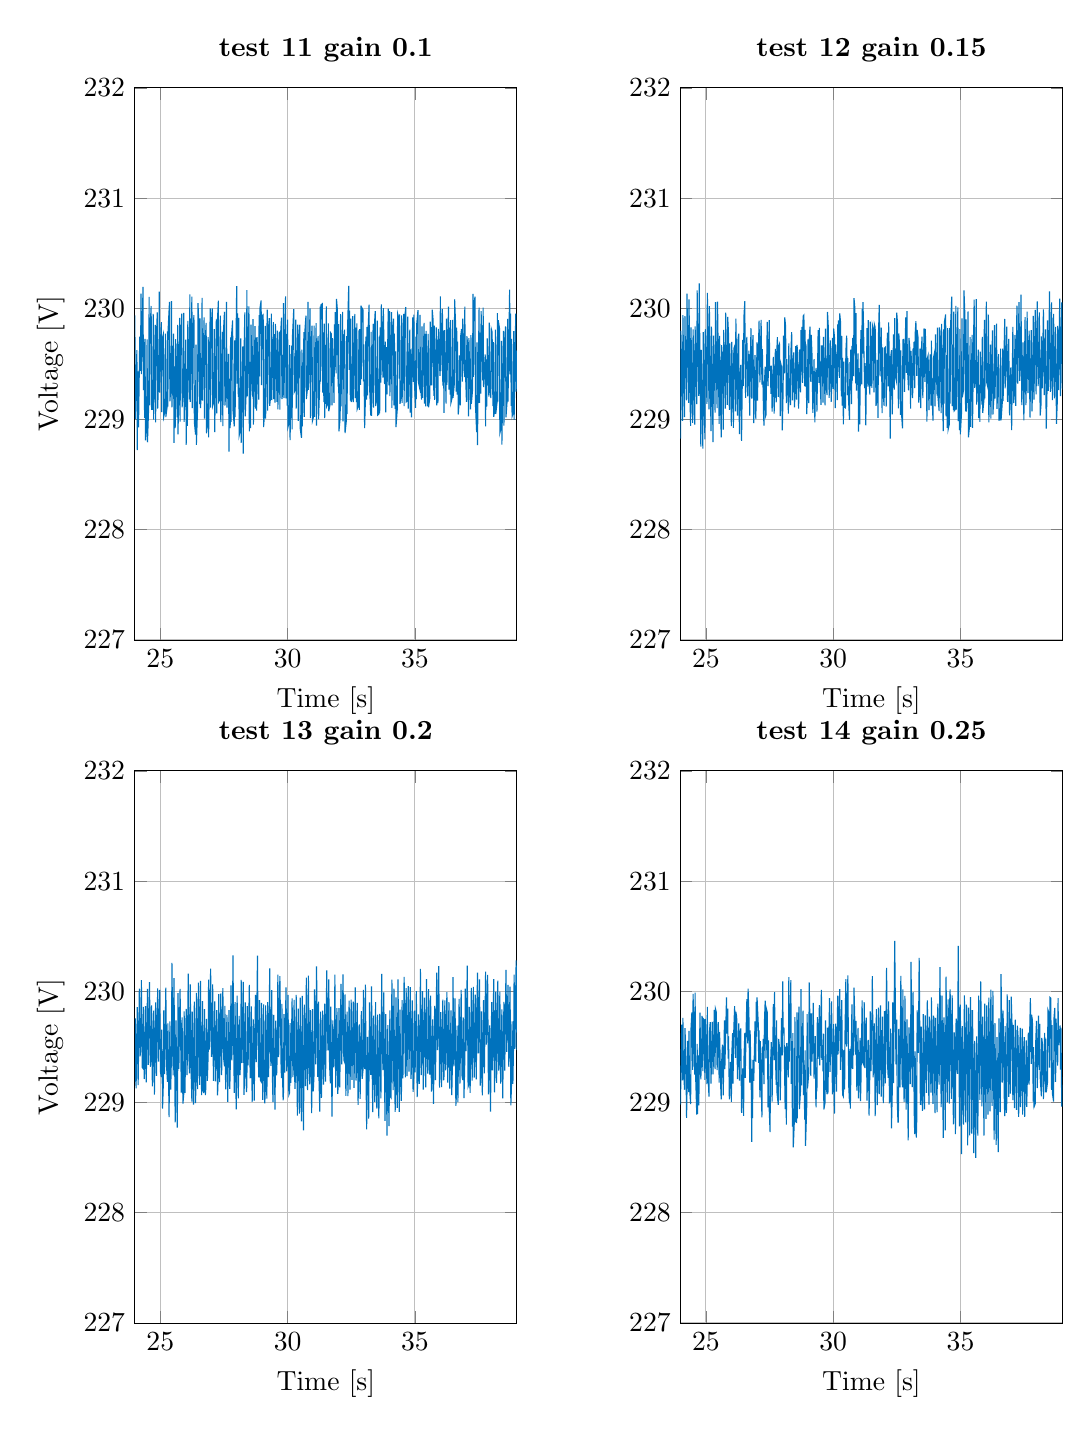
\begin{tikzpicture}

\begin{axis}[%
width=0.4\textwidth,
height=2.761in,
at={(1.272in,4.208in)},
scale only axis,
xmin=24,
xmax=39,
xlabel={Time [s]},
xmajorgrids,
ymin=227,
ymax=232,
ylabel={Voltage [V]},
ymajorgrids,
axis background/.style={fill=white},
title style={font=\bfseries},
title={test 11 gain 0.1}
]
\addplot [color=mycolor1,solid,forget plot]
  table[row sep=crcr]{%
24	229.940619430066\\
24.016	229.001681330484\\
24.08	229.624908225122\\
24.096	228.719850414882\\
24.112	229.432686385489\\
24.144	228.925305964881\\
24.192	229.746925731247\\
24.224	229.437440998499\\
24.24	230.137406874724\\
24.256	229.407524265201\\
24.32	230.198300420818\\
24.336	229.263753496733\\
24.352	229.696732389536\\
24.384	229.011560249812\\
24.4	229.727552555512\\
24.416	228.808203798408\\
24.464	228.967075441542\\
24.48	229.722951814731\\
24.496	228.791244863064\\
24.544	229.127657210736\\
24.56	230.106396321719\\
24.576	229.128360974804\\
24.592	229.793683943921\\
24.64	230.024748717813\\
24.656	229.088769064326\\
24.704	229.090103476621\\
24.72	229.953747035177\\
24.736	228.997136125006\\
24.8	229.854843023014\\
24.816	228.971451400557\\
24.832	229.640600696375\\
24.88	229.966930999648\\
24.896	229.096163653492\\
24.944	229.45140468999\\
24.96	230.154385308134\\
24.976	229.240149396444\\
25.04	229.879652949904\\
25.056	229.064766718713\\
25.072	229.723396809675\\
25.12	229.77034037568\\
25.136	229.023293907224\\
25.184	229.078833159746\\
25.2	229.7751124765\\
25.216	229.019234327572\\
25.264	229.104037862447\\
25.28	229.794025114744\\
25.296	229.114155818692\\
25.312	229.838615512214\\
25.36	230.06283319001\\
25.376	229.161984480307\\
25.424	229.318154590361\\
25.44	230.070116092887\\
25.456	229.106900030391\\
25.52	229.774258672626\\
25.536	228.785349152781\\
25.552	229.477783600867\\
25.584	228.919401076568\\
25.6	229.723743420818\\
25.664	229.01558421774\\
25.68	229.854205108247\\
25.696	228.862036416246\\
25.76	229.918104886264\\
25.776	228.977780444858\\
25.792	229.642502491109\\
25.84	229.956420482688\\
25.856	229.106192109832\\
25.904	229.287169667045\\
25.92	229.961761888142\\
25.936	228.976050196397\\
26	229.72141321291\\
26.016	228.766434072724\\
26.032	229.456015978056\\
26.064	228.938480852947\\
26.08	229.890346170459\\
26.144	229.180357113568\\
26.16	230.130092496167\\
26.176	229.156900314669\\
26.24	230.109743673075\\
26.256	229.099365122625\\
26.272	229.715239712733\\
26.32	229.941747954007\\
26.336	228.976616379965\\
26.384	228.860736721519\\
26.4	229.675942403105\\
26.416	228.766721368489\\
26.464	229.099266023174\\
26.48	230.049743271828\\
26.512	229.866679125185\\
26.544	229.135512111442\\
26.56	229.912663802331\\
26.576	229.099397144927\\
26.624	229.2850738422\\
26.64	230.097590774775\\
26.656	229.169086530093\\
26.72	229.921177325124\\
26.736	229.005190653816\\
26.752	229.644430051095\\
26.8	229.871512485622\\
26.816	228.871602752589\\
26.864	228.993569686574\\
26.88	229.743452119174\\
26.896	228.835574778926\\
26.96	230.003228098837\\
26.976	229.104661469276\\
26.992	229.793359179614\\
27.04	230.002385650566\\
27.056	229.120687163881\\
27.104	229.160192698897\\
27.12	229.815125985883\\
27.136	228.881945257949\\
27.2	229.90376669774\\
27.216	229.051591813404\\
27.232	229.835592697705\\
27.28	230.073168961951\\
27.296	229.159111336588\\
27.344	229.182817325237\\
27.36	229.937362123723\\
27.376	228.97254754337\\
27.44	229.789762622176\\
27.456	228.936851475152\\
27.472	229.758505095726\\
27.52	229.972602910496\\
27.536	229.122660632125\\
27.584	229.270874876395\\
27.6	230.061871530043\\
27.616	229.103646677457\\
27.68	229.590732609942\\
27.696	228.70737632534\\
27.712	229.366052572441\\
27.744	228.917990895196\\
27.76	229.739743891186\\
27.776	228.974996357851\\
27.792	229.743860229613\\
27.84	229.893808371956\\
27.856	229.074331897851\\
27.904	228.934136383277\\
27.92	229.714695333356\\
27.936	229.018974014691\\
28	230.204642647313\\
28.016	229.322009734706\\
28.032	229.958042779714\\
28.064	229.203098612185\\
28.08	229.916694856973\\
28.096	228.85203511806\\
28.144	228.903307579557\\
28.16	229.732438563127\\
28.176	228.784881430157\\
28.24	229.659330790504\\
28.256	228.688156108701\\
28.272	229.401841990186\\
28.32	229.966459795791\\
28.336	229.025216383795\\
28.384	229.325342899167\\
28.4	230.169035587049\\
28.416	229.207445741729\\
28.48	230.021627717842\\
28.496	228.890092709863\\
28.512	229.519588579577\\
28.544	228.919599714316\\
28.56	229.855881936423\\
28.624	229.204071907764\\
28.64	229.906025668526\\
28.656	228.951425821506\\
28.72	229.84366128554\\
28.736	229.094868431694\\
28.752	229.739313888234\\
28.784	229.077939394025\\
28.8	229.742738404382\\
28.864	229.177292199619\\
28.88	229.942754903949\\
28.896	229.386821664612\\
28.912	230.002465505458\\
28.96	230.075928758328\\
28.976	229.308011154657\\
28.992	229.934331114083\\
29.04	229.945369153102\\
29.056	228.929037341186\\
29.104	229.090493477009\\
29.12	229.845439835385\\
29.136	229.004935076327\\
29.2	229.99127055277\\
29.216	229.078592169772\\
29.232	229.774880990477\\
29.28	229.914917478438\\
29.296	229.121151288332\\
29.344	229.229101025848\\
29.36	229.955096694932\\
29.376	229.173758727486\\
29.44	229.878975833846\\
29.456	229.182158351594\\
29.472	229.769136026102\\
29.504	229.150926411121\\
29.52	229.863455986354\\
29.584	229.157768762826\\
29.6	229.800785658454\\
29.616	229.088110854672\\
29.68	229.793827463751\\
29.696	229.087702374689\\
29.712	229.720093282721\\
29.76	229.919778850274\\
29.776	229.182088124765\\
29.824	229.266696417465\\
29.84	230.051693523199\\
29.856	229.190792254017\\
29.92	230.112241198394\\
29.936	229.189148601751\\
29.952	229.770028036765\\
29.984	229.122866167831\\
30	229.901776890767\\
30.016	228.930884240898\\
30.064	228.976538425022\\
30.08	229.671691564415\\
30.096	228.811359342027\\
30.16	229.664966472904\\
30.176	228.907391526068\\
30.192	229.757207334667\\
30.24	229.996355471166\\
30.256	229.243003047129\\
30.304	229.268872221281\\
30.32	229.900938656679\\
30.336	229.094967976786\\
30.4	229.856357554938\\
30.416	228.984809254373\\
30.432	229.66397293916\\
30.48	229.856470366601\\
30.496	228.915075405261\\
30.544	228.832022791082\\
30.56	229.629640015189\\
30.576	228.935695208302\\
30.64	229.788642165399\\
30.656	229.020798242467\\
30.672	229.778604031076\\
30.72	229.936544090782\\
30.736	229.182894310968\\
30.784	229.286457491298\\
30.8	230.062977301986\\
30.816	229.26479027206\\
30.88	230.0027017598\\
30.896	229.0094096211\\
30.912	229.614681414055\\
30.96	229.846046069474\\
30.976	228.985406786474\\
31.024	229.02697696764\\
31.04	229.847532016554\\
31.056	229.020548129858\\
31.12	229.870133725687\\
31.136	228.941232293898\\
31.152	229.604926094836\\
31.2	229.752714435997\\
31.216	228.997869429084\\
31.264	229.348529555096\\
31.28	230.019794213454\\
31.296	229.34033324048\\
31.312	230.035608667327\\
31.36	230.044504457733\\
31.376	229.241102494648\\
31.392	229.785620183474\\
31.424	229.154759047639\\
31.44	229.864824839971\\
31.456	229.009002093699\\
31.472	229.672278394818\\
31.504	229.138779348843\\
31.52	230.020716797389\\
31.536	229.116373007921\\
31.584	229.142845847086\\
31.6	229.866998827999\\
31.616	229.072382202451\\
31.664	229.129334367142\\
31.68	229.7855118572\\
31.712	229.774281947307\\
31.744	229.124033812876\\
31.76	229.733612538179\\
31.824	229.14728059356\\
31.84	229.857483478092\\
31.856	229.473054946745\\
31.872	229.970269921771\\
31.904	229.414817532547\\
31.92	230.088160800246\\
31.952	229.997482947826\\
31.984	229.295521791045\\
32	229.861424858059\\
32.016	228.890673831414\\
32.064	229.011374703891\\
32.08	229.951089918723\\
32.096	229.116182402261\\
32.16	229.970773510826\\
32.176	228.981044065725\\
32.192	229.657045975343\\
32.24	229.811410901746\\
32.256	228.874933450876\\
32.304	228.980930460867\\
32.32	229.75098577824\\
32.336	229.045538546005\\
32.352	229.802750212839\\
32.4	230.206665999842\\
32.416	229.446346494212\\
32.432	229.983085893106\\
32.464	229.168815421894\\
32.48	229.910899782756\\
32.496	229.155744860563\\
32.544	229.212021044256\\
32.56	229.932852432428\\
32.576	229.154400439314\\
32.64	229.952366423197\\
32.656	229.191526229614\\
32.672	229.828929438182\\
32.704	229.154434389359\\
32.72	229.867326101994\\
32.736	229.093966204135\\
32.784	229.128015650636\\
32.8	229.803724795582\\
32.816	229.083348833307\\
32.832	229.815229887492\\
32.864	229.311291505806\\
32.88	230.027738014191\\
32.896	229.362170974826\\
32.912	230.010827389287\\
32.96	229.990656631599\\
32.976	229.342329404624\\
32.992	229.677216064746\\
33.024	228.919255416821\\
33.056	229.18246410732\\
33.072	229.746987595942\\
33.104	229.176722199568\\
33.12	229.836778818831\\
33.136	229.214666624087\\
33.152	229.754616325109\\
33.2	230.036281742499\\
33.216	229.310562619292\\
33.264	229.034514391332\\
33.28	229.79127366223\\
33.296	229.030753595817\\
33.36	229.86274948768\\
33.376	229.105540592264\\
33.392	229.770308922881\\
33.44	229.978639369825\\
33.456	229.118952638071\\
33.504	229.18254687888\\
33.52	229.892920170364\\
33.536	229.036381533867\\
33.584	229.045893050081\\
33.6	229.747570471368\\
33.616	229.052348227102\\
33.632	229.831328617162\\
33.664	229.330260565069\\
33.68	230.039312488709\\
33.744	229.376057129427\\
33.76	230.005750453574\\
33.808	229.317431951472\\
33.84	229.702831410521\\
33.856	229.061084428208\\
33.872	229.651319136524\\
33.904	229.224916878054\\
33.952	230.000318137712\\
33.984	229.307292876262\\
34	229.979116949154\\
34.016	229.209295771598\\
34.08	229.969849503184\\
34.096	229.102285987864\\
34.112	229.764504552819\\
34.16	229.910659270851\\
34.176	229.126192096826\\
34.192	229.775404098473\\
34.224	229.092858444925\\
34.24	229.613089099385\\
34.256	228.928084496958\\
34.304	229.081392127092\\
34.32	229.956938220655\\
34.352	229.928657403788\\
34.384	229.366220890229\\
34.4	229.950121823403\\
34.416	229.13897575381\\
34.464	229.225576004336\\
34.48	229.940201469146\\
34.496	229.147180042161\\
34.56	229.954476618694\\
34.576	229.118898042793\\
34.592	229.900619500749\\
34.64	230.015431208917\\
34.656	229.156291146739\\
34.704	229.169018372649\\
34.72	229.928362762701\\
34.736	229.095206692505\\
34.8	229.810361346596\\
34.816	229.060299678975\\
34.832	229.631170467093\\
34.864	229.016115978586\\
34.912	229.921841914272\\
34.944	229.338160836035\\
34.96	229.947018937047\\
34.976	229.36553060504\\
35.024	229.1017544534\\
35.04	229.748004662698\\
35.056	229.180928587443\\
35.072	229.865123540788\\
35.12	229.987783287866\\
35.136	229.336204308412\\
35.184	229.284153665038\\
35.2	229.944867601081\\
35.216	229.300719148353\\
35.264	229.17791663443\\
35.28	229.841180402466\\
35.296	229.192485856619\\
35.36	229.872636582555\\
35.376	229.141413633175\\
35.392	229.772331353504\\
35.424	229.115373874509\\
35.44	229.800419880613\\
35.504	229.115417051251\\
35.52	229.773520381641\\
35.536	229.107596410698\\
35.584	229.190809447673\\
35.6	229.884100211944\\
35.616	229.305046664807\\
35.632	229.834433586004\\
35.664	229.30544145259\\
35.68	229.992197205193\\
35.712	229.904563269696\\
35.744	229.210852327766\\
35.76	229.847021556625\\
35.776	229.175985025024\\
35.84	229.831514486277\\
35.856	229.125196016242\\
35.872	229.720534255907\\
35.904	229.144838424352\\
35.92	229.818458521072\\
35.984	229.392803041847\\
36	230.112020749704\\
36.016	229.436139790582\\
36.08	229.998405761213\\
36.096	229.304412264751\\
36.112	229.801403846622\\
36.144	229.058169397856\\
36.16	229.805251454573\\
36.224	229.141162816629\\
36.24	229.910082229558\\
36.256	229.311206362396\\
36.32	230.01996769151\\
36.336	229.267111379562\\
36.352	229.828673443264\\
36.384	229.221867186072\\
36.4	229.896552888871\\
36.416	229.149720397638\\
36.464	229.196363270742\\
36.48	229.899952077991\\
36.496	229.194006094322\\
36.544	229.310027481345\\
36.56	230.085834096126\\
36.592	229.894332120052\\
36.624	229.249678250389\\
36.64	229.829309327612\\
36.656	229.222936776084\\
36.672	229.702837057657\\
36.704	229.042650979903\\
36.736	229.155533595422\\
36.752	229.57809536486\\
36.784	229.125062520557\\
36.8	229.755852624975\\
36.832	229.816324622489\\
36.864	229.34119275832\\
36.88	229.911446070491\\
36.944	229.380019060376\\
36.96	230.018677790477\\
36.976	229.494335468601\\
37.024	229.157353289805\\
37.04	229.751669368146\\
37.072	229.677879436378\\
37.104	229.02552353667\\
37.12	229.734031261155\\
37.184	229.088145759805\\
37.2	229.760897984903\\
37.216	229.139813347686\\
37.264	229.26305748167\\
37.28	230.134115419709\\
37.296	229.383950099524\\
37.312	230.024398721548\\
37.36	230.109133262102\\
37.376	229.139657467927\\
37.424	228.883144476587\\
37.44	229.695131353771\\
37.456	228.766082050482\\
37.52	230.009068173266\\
37.536	229.147040597686\\
37.552	229.7829105265\\
37.584	229.231520061003\\
37.6	229.978533044249\\
37.664	229.351895400394\\
37.68	230.009674268391\\
37.696	229.290058576424\\
37.76	229.586827484148\\
37.776	228.935574468329\\
37.792	229.542166749666\\
37.824	229.114901665809\\
37.84	229.731445065326\\
37.904	229.204134001049\\
37.92	229.873975369951\\
37.936	229.289800689696\\
37.984	229.191717754074\\
38	229.816174153709\\
38.032	229.789836237454\\
38.064	229.11871758415\\
38.08	229.697590149903\\
38.096	229.021489971082\\
38.144	229.097016088707\\
38.16	229.810930302907\\
38.176	229.04727183036\\
38.224	229.148798448608\\
38.24	229.96099847578\\
38.256	229.159092547516\\
38.272	229.895951948887\\
38.32	229.825116931325\\
38.336	228.874037963045\\
38.384	228.920814462032\\
38.4	229.709707490159\\
38.416	228.770540112982\\
38.48	229.80055960627\\
38.496	228.94206772927\\
38.512	229.60113421164\\
38.56	229.839661455268\\
38.576	229.016893240435\\
38.624	229.17546962552\\
38.64	229.907370862392\\
38.656	229.15907153628\\
38.72	230.173946995693\\
38.736	229.406281616067\\
38.752	229.955789122182\\
38.784	229.120906536709\\
38.8	229.727695389759\\
38.816	229.024760155513\\
38.864	229.060673153496\\
38.88	229.797029594953\\
38.896	228.99392659391\\
38.96	229.956827391266\\
38.976	229.249733582657\\
39.008	229.619730321007\\
};
\end{axis}

\begin{axis}[%
width=0.4\textwidth,
height=2.761in,
at={(4in,4.208in)},
scale only axis,
xmin=24,
xmax=39,
xlabel={Time [s]},
xmajorgrids,
ymin=227,
ymax=232,
ymajorgrids,
axis background/.style={fill=white},
title style={font=\bfseries},
title={test 12  gain 0.15}
]
\addplot [color=mycolor1,solid,forget plot]
  table[row sep=crcr]{%
24	228.824607800195\\
24.016	229.802125762676\\
24.08	228.983825529026\\
24.096	229.94281114685\\
24.144	229.188103168088\\
24.16	229.019417135161\\
24.176	229.932451339055\\
24.192	229.645091148349\\
24.24	229.169455971502\\
24.256	230.136053837118\\
24.32	229.148767323501\\
24.336	230.084178470652\\
24.384	229.088321155939\\
24.4	228.939633624411\\
24.416	229.832269814839\\
24.432	229.500182578303\\
24.48	228.965781049393\\
24.496	229.812283349268\\
24.56	228.949815404299\\
24.576	229.840567415716\\
24.624	229.272593041991\\
24.64	229.136891528544\\
24.656	230.166979456362\\
24.672	229.868668918851\\
24.72	229.210564847842\\
24.736	230.230751699879\\
24.8	228.751812770902\\
24.816	229.628152363245\\
24.864	228.904347187222\\
24.88	228.734291937985\\
24.896	229.787835293984\\
24.912	229.54612614903\\
24.96	228.816538066559\\
24.976	229.814250225543\\
25.04	229.138214049986\\
25.056	230.143779111124\\
25.104	229.488246215907\\
25.12	229.088621821698\\
25.136	230.024732133402\\
25.152	229.673105665291\\
25.2	228.891167325971\\
25.216	229.838534831176\\
25.28	228.791958892913\\
25.296	229.755554172104\\
25.344	229.347092942641\\
25.36	229.058793721274\\
25.376	230.059809866494\\
25.392	229.727144051612\\
25.44	229.09972633529\\
25.456	230.064356885624\\
25.52	228.958210955402\\
25.536	229.755358136232\\
25.584	229.042246263451\\
25.6	228.835451103995\\
25.616	229.670610877737\\
25.648	229.522563307323\\
25.68	228.906173439968\\
25.696	229.807778986038\\
25.76	229.095225212541\\
25.776	229.963808080512\\
25.824	229.276508055963\\
25.84	229.129045491352\\
25.856	229.927153935957\\
25.888	229.768193102507\\
25.92	229.085060224996\\
25.936	229.686319780443\\
26	228.938117237676\\
26.016	229.700083853279\\
26.064	229.116049987574\\
26.08	228.922100311572\\
26.096	229.638987419433\\
26.128	229.659890016942\\
26.16	229.069770080807\\
26.176	229.910889471019\\
26.24	229.032760778291\\
26.256	229.713982923494\\
26.288	229.774304990797\\
26.304	229.065407215348\\
26.32	228.86399574404\\
26.336	229.380847135008\\
26.368	229.491930193756\\
26.4	228.803937486844\\
26.448	229.716981543318\\
26.464	229.298855463458\\
26.496	229.9402401122\\
26.528	230.069146666808\\
26.544	229.407267177479\\
26.56	229.191917251972\\
26.576	229.565228166755\\
26.608	229.746056514378\\
26.64	229.206330700148\\
26.688	229.621466499624\\
26.72	229.032650677637\\
26.736	229.32301936151\\
26.768	229.824244478581\\
26.8	229.187151125138\\
26.816	229.567024704363\\
26.848	229.760315143296\\
26.88	228.963409042039\\
26.928	229.578987390676\\
26.96	229.001433463635\\
27.008	229.696517624621\\
27.024	229.169125500187\\
27.056	229.566701006848\\
27.088	229.892983936405\\
27.12	229.332713247666\\
27.168	229.900053987547\\
27.2	229.312013652895\\
27.216	229.633497349755\\
27.264	229.039861365855\\
27.28	228.941793105038\\
27.296	229.313348903056\\
27.328	229.47604285635\\
27.344	229.028818749746\\
27.36	229.039745404587\\
27.408	229.880111248931\\
27.44	229.299369926425\\
27.488	229.897381073911\\
27.504	229.436552596865\\
27.536	229.480075752547\\
27.552	229.230268671493\\
27.568	229.485226442845\\
27.6	229.068014097977\\
27.648	229.564736721429\\
27.68	229.051402344342\\
27.728	229.637058920282\\
27.744	229.278912959325\\
27.76	229.151932514596\\
27.776	229.573450421876\\
27.808	229.742254842914\\
27.824	229.385720904964\\
27.84	229.201571181151\\
27.856	229.658246131373\\
27.888	229.68009055397\\
27.92	229.027517219067\\
27.936	229.506951853143\\
27.968	229.476168624086\\
28	228.897869046269\\
28.032	229.2546342644\\
28.048	229.756941136042\\
28.08	229.413934790863\\
28.096	229.922122354178\\
28.128	229.845970806176\\
28.16	229.145827604407\\
28.176	229.544695575319\\
28.24	229.051438805904\\
28.256	229.685360422067\\
28.272	229.344218049852\\
28.32	229.126455515165\\
28.336	229.59890669744\\
28.368	229.788182205485\\
28.4	229.171009581591\\
28.448	229.604510045137\\
28.48	229.107540262825\\
28.512	229.342258306444\\
28.528	229.661678050925\\
28.56	229.177399964554\\
28.576	229.671982421649\\
28.608	229.599123396043\\
28.64	229.095837147583\\
28.688	229.632615163357\\
28.72	229.243501344358\\
28.736	229.806452991658\\
28.752	229.430403687405\\
28.768	229.835808839236\\
28.8	229.328012337521\\
28.816	229.93331038638\\
28.848	229.942868307241\\
28.88	229.299516406643\\
28.896	229.807847889578\\
28.912	229.295803947379\\
28.928	229.681923595212\\
28.96	229.045083766711\\
28.992	229.270823338392\\
29.008	229.722188723943\\
29.04	229.146474679161\\
29.056	229.713204070037\\
29.088	229.838782037321\\
29.12	229.337365277714\\
29.136	229.762531217858\\
29.168	229.578065636293\\
29.2	229.056366546592\\
29.248	229.542994273692\\
29.264	229.181025084004\\
29.28	228.971664428815\\
29.296	229.363169504309\\
29.328	229.464677376908\\
29.36	229.069095510704\\
29.408	229.806555292684\\
29.44	229.328372146341\\
29.456	229.826535134093\\
29.472	229.443807390167\\
29.52	229.130284434682\\
29.536	229.663916182916\\
29.568	229.663226988403\\
29.6	229.150433243154\\
29.616	229.745121279016\\
29.68	229.126021393688\\
29.696	229.820857354465\\
29.712	229.310437330557\\
29.76	229.218410697475\\
29.776	229.970405062584\\
29.808	229.829875796777\\
29.84	229.194054717437\\
29.888	229.713285234054\\
29.92	229.157470431475\\
29.952	229.370084232493\\
29.968	229.736472473051\\
30	229.273488755428\\
30.016	229.82098058935\\
30.048	229.749228387222\\
30.08	229.101240838944\\
30.096	229.677470581481\\
30.16	229.171773473479\\
30.176	229.858425536287\\
30.192	229.470471992439\\
30.208	229.894223753127\\
30.24	229.374492638705\\
30.256	229.957323889733\\
30.288	229.878105077384\\
30.32	229.206050194229\\
30.336	229.752046791464\\
30.352	229.123542056622\\
30.368	229.554614969998\\
30.4	228.953491738031\\
30.416	229.521690228585\\
30.432	229.111825758538\\
30.48	229.102929076913\\
30.496	229.607456877353\\
30.528	229.755774790523\\
30.56	229.218951397753\\
30.576	229.552391206731\\
30.592	229.217566995314\\
30.64	228.993833277426\\
30.656	229.515986416554\\
30.672	229.259831086087\\
30.688	229.629669923368\\
30.72	229.136666541144\\
30.736	229.664776341151\\
30.752	229.349660791371\\
30.768	229.737185447823\\
30.8	229.390304405263\\
30.816	230.095030484474\\
30.848	230.012817362633\\
30.88	229.323196020829\\
30.896	229.960209295065\\
30.912	229.258222521231\\
30.976	229.596101346058\\
30.992	228.886374670905\\
31.008	229.462641461553\\
31.04	228.9519500928\\
31.088	229.806453345857\\
31.12	229.315320231437\\
31.136	229.999656043201\\
31.152	229.592716867562\\
31.168	230.060460012896\\
31.184	229.915264880011\\
31.232	229.281153001325\\
31.248	229.506745143991\\
31.28	228.943658719657\\
31.328	229.824894002131\\
31.36	229.294742315301\\
31.376	229.897687312726\\
31.392	229.404332200369\\
31.44	229.223039894802\\
31.456	229.884375273898\\
31.472	229.300267247501\\
31.488	229.753660977526\\
31.52	229.283996137418\\
31.536	229.853243672421\\
31.568	229.819723023929\\
31.6	229.243236045527\\
31.616	229.859390222568\\
31.648	229.831691135071\\
31.68	229.120452800646\\
31.712	229.167964212327\\
31.728	229.536521819596\\
31.76	229.011067580962\\
31.776	229.744210816997\\
31.808	230.034635852725\\
31.84	229.387582615264\\
31.888	229.829309903946\\
31.92	229.054658195782\\
31.936	229.650562139631\\
31.952	229.256112026156\\
32	229.12040619708\\
32.016	229.643029497568\\
32.048	229.651497975865\\
32.08	229.113236360488\\
32.128	229.783293259524\\
32.16	229.296422423631\\
32.176	229.87669523287\\
32.224	229.23011832759\\
32.24	228.825071768107\\
32.256	229.558813745951\\
32.288	229.624453574652\\
32.32	229.043166892959\\
32.368	229.767750516064\\
32.4	229.268700957037\\
32.416	229.914148292088\\
32.432	229.396535510306\\
32.48	229.346653720442\\
32.496	229.964791673515\\
32.528	229.855273807105\\
32.56	229.09837755336\\
32.576	229.775673198245\\
32.608	229.661629739684\\
32.64	229.038840605376\\
32.656	229.623808291768\\
32.672	229.093017223479\\
32.72	228.917416520128\\
32.736	229.718632982074\\
32.768	229.722243256052\\
32.8	229.247892475733\\
32.848	229.920901818385\\
32.88	229.419310314405\\
32.896	229.978296723622\\
32.912	229.480242230967\\
32.96	229.260870201509\\
32.976	229.736124406612\\
33.008	229.642005720138\\
33.04	229.095225444627\\
33.056	229.618096972935\\
33.12	229.190344904179\\
33.136	229.641839752366\\
33.152	229.394673994357\\
33.168	229.699477890671\\
33.2	229.281626769185\\
33.216	229.761346553203\\
33.248	229.887076600367\\
33.28	229.392317183053\\
33.296	229.807515240272\\
33.328	229.747116471003\\
33.36	229.150199179342\\
33.392	229.248121704031\\
33.408	229.638033238792\\
33.44	229.100199873361\\
33.456	229.593086783982\\
33.488	229.747216710172\\
33.52	229.19138149104\\
33.568	229.822755593724\\
33.6	229.33893626187\\
33.616	229.816597411864\\
33.664	229.331068702651\\
33.68	228.97889710579\\
33.696	229.550549890436\\
33.728	229.57755410504\\
33.76	229.081041501646\\
33.808	229.587393231912\\
33.84	229.121905392089\\
33.856	229.711016785661\\
33.872	229.250431679822\\
33.92	228.986556166225\\
33.936	229.552281190284\\
33.968	229.58996978042\\
34	229.116646763267\\
34.016	229.767538921188\\
34.08	229.2136211352\\
34.096	229.829846702266\\
34.112	229.208250659248\\
34.16	229.073494210687\\
34.176	229.830986883227\\
34.208	229.679651667214\\
34.24	229.055185381729\\
34.256	229.862610706802\\
34.32	228.89163810289\\
34.336	229.81253258403\\
34.352	229.141642451407\\
34.368	229.880831011172\\
34.416	229.948401973934\\
34.432	229.024407480189\\
34.448	229.580540513912\\
34.48	228.920781488413\\
34.496	229.824493913767\\
34.512	228.904518447514\\
34.56	228.954778885769\\
34.576	229.825593685933\\
34.592	229.140612895655\\
34.608	229.836762758557\\
34.656	230.110609895094\\
34.672	229.119198338783\\
34.688	229.674652270459\\
34.72	229.081731036607\\
34.736	229.973522430104\\
34.752	229.075637063803\\
34.8	229.089923634847\\
34.816	230.02498811757\\
34.832	229.087226641502\\
34.896	230.013044805569\\
34.912	228.983380381186\\
34.928	229.452722772305\\
34.96	228.902780666928\\
34.976	229.816053783761\\
34.992	228.863458579847\\
35.04	229.059301217087\\
35.056	229.912676860257\\
35.072	229.198523345298\\
35.12	229.267548655769\\
35.136	230.1657286943\\
35.168	229.961334375579\\
35.2	229.070275725224\\
35.216	229.903793405703\\
35.232	229.0682247065\\
35.248	229.688079022531\\
35.28	229.14871110233\\
35.296	229.975140436395\\
35.312	228.836286647525\\
35.36	228.952457195607\\
35.376	229.742994668239\\
35.392	228.930566757605\\
35.456	229.763426750329\\
35.472	228.921502397843\\
35.504	229.569684075611\\
35.536	230.083091455727\\
35.552	229.282986981411\\
35.6	229.400473567517\\
35.616	230.087130661053\\
35.632	229.131883952113\\
35.696	229.629921190774\\
35.712	229.008992613051\\
35.744	229.308841345985\\
35.76	228.975818758217\\
35.776	229.611124012491\\
35.84	229.133017968977\\
35.856	229.74425177253\\
35.872	229.056453592746\\
35.92	229.172507844293\\
35.936	229.900318837851\\
35.952	229.188155853791\\
35.984	229.659359279143\\
36.016	230.064135766743\\
36.032	229.329798163976\\
36.08	229.281847320966\\
36.096	229.947629923416\\
36.112	228.971797478693\\
36.176	229.675384027214\\
36.192	229.004429921114\\
36.224	229.406706340201\\
36.256	229.804944846762\\
36.272	229.040886571944\\
36.32	229.238615136\\
36.336	229.851164908537\\
36.352	229.187042541922\\
36.416	229.864153750202\\
36.432	229.093987792186\\
36.464	229.278030016077\\
36.496	229.588221393741\\
36.512	228.991675128221\\
36.56	228.993456727415\\
36.576	229.638930399727\\
36.592	228.988543758273\\
36.64	229.148558708042\\
36.656	229.639452447971\\
36.672	229.163208926817\\
36.704	229.526291595872\\
36.736	229.907103602764\\
36.752	229.279646380698\\
36.768	229.369954642003\\
36.816	229.839040559614\\
36.848	229.157864056426\\
36.896	229.727122402868\\
36.912	229.195598148566\\
36.928	229.03398116054\\
36.944	229.255020651861\\
36.976	229.470010066\\
37.008	228.901144553378\\
37.056	229.836405486698\\
37.088	229.145309534156\\
37.12	229.243424523856\\
37.136	229.761016346893\\
37.168	229.120517005738\\
37.184	229.499545950282\\
37.216	230.027290695533\\
37.248	229.321499622147\\
37.296	230.060430308079\\
37.328	229.347668010164\\
37.36	229.562771094349\\
37.376	230.128723959783\\
37.392	229.589765880277\\
37.408	229.126797175051\\
37.456	229.694836635238\\
37.488	228.989868220858\\
37.536	229.92357840932\\
37.568	229.128330119277\\
37.6	229.483100777422\\
37.616	229.973470942391\\
37.632	229.647843673059\\
37.648	229.235214109356\\
37.696	229.801590033946\\
37.728	229.015306818642\\
37.776	229.806202811769\\
37.808	229.071548003284\\
37.84	229.396429216152\\
37.856	229.935086164081\\
37.888	229.177972174018\\
37.904	229.575805103839\\
37.936	229.989365289888\\
37.968	229.223680268593\\
38.016	230.067458132705\\
38.048	229.29997616933\\
38.08	229.488912889413\\
38.096	229.968143852694\\
38.112	229.491516390555\\
38.128	229.031725618494\\
38.16	229.125215098655\\
38.176	229.749608567257\\
38.208	229.279845196442\\
38.256	229.99467795733\\
38.288	229.217968022389\\
38.336	229.813227555288\\
38.352	229.257697240719\\
38.368	228.913792269113\\
38.4	229.290055077441\\
38.416	229.89507218355\\
38.448	229.255665314109\\
38.496	230.157579342515\\
38.528	229.247346786231\\
38.56	229.473539925171\\
38.576	230.05666492482\\
38.592	229.614415820728\\
38.608	229.173245736244\\
38.656	229.952773612959\\
38.688	229.188717833739\\
38.736	229.835612011757\\
38.768	228.958396828734\\
38.8	229.149897771753\\
38.816	229.844552828253\\
38.848	229.263113148186\\
38.864	229.530470293664\\
38.896	230.092443873367\\
38.928	229.208663792847\\
38.976	230.057085704133\\
39.008	229.268486954306\\
};
\end{axis}

\begin{axis}[%
width=0.4\textwidth,
height=2.761in,
at={(1.272in,0.793in)},
scale only axis,
xmin=24,
xmax=39,
xlabel={Time [s]},
xmajorgrids,
ymin=227,
ymax=232,
ylabel={Voltage [V]},
ymajorgrids,
axis background/.style={fill=white},
title style={font=\bfseries},
title={test 13  gain 0.2}
]
\addplot [color=mycolor1,solid,forget plot]
  table[row sep=crcr]{%
24	229.185430723113\\
24.016	229.758505008503\\
24.048	229.125972202739\\
24.096	229.8612106098\\
24.128	229.155484714398\\
24.144	229.419078287725\\
24.176	230.027866186632\\
24.208	229.414319798051\\
24.24	229.661641148025\\
24.256	230.104808833219\\
24.288	229.31522870354\\
24.32	229.30561813673\\
24.336	229.862632647963\\
24.368	229.210113404833\\
24.4	229.371130508957\\
24.416	229.869198995289\\
24.432	229.613337644699\\
24.448	229.178962706781\\
24.496	230.025100394251\\
24.528	229.33749072925\\
24.576	230.086964935717\\
24.608	229.32113674583\\
24.64	229.417581108287\\
24.656	229.875782999049\\
24.672	229.45849516197\\
24.688	229.14368350147\\
24.736	229.829578524405\\
24.768	229.06894267129\\
24.816	229.9035449051\\
24.848	229.237867561323\\
24.864	229.500356046741\\
24.896	230.029875567133\\
24.912	229.758451012881\\
24.928	229.367835019826\\
24.976	230.016948627685\\
25.008	229.272858686514\\
25.04	229.228133762905\\
25.056	229.656421092236\\
25.088	228.941297504546\\
25.12	229.177578062872\\
25.136	229.830626216109\\
25.152	229.528910520197\\
25.168	229.254480392463\\
25.216	230.037318052408\\
25.248	229.312564728909\\
25.28	229.184332432169\\
25.296	229.713181595641\\
25.344	228.86583347603\\
25.376	229.731712461528\\
25.408	229.11458374282\\
25.44	229.444863785713\\
25.456	230.262483392765\\
25.504	229.24366046675\\
25.536	230.124092954092\\
25.584	228.817592210498\\
25.616	229.740063304025\\
25.664	228.768941469347\\
25.68	229.156176073355\\
25.696	229.988586278521\\
25.728	229.302197642478\\
25.776	230.026002871015\\
25.824	229.08769357631\\
25.856	229.768911604276\\
25.872	229.278463816169\\
25.888	228.986373675313\\
25.92	229.072873106744\\
25.936	229.82222128386\\
25.968	229.084333020455\\
26.016	229.84535216948\\
26.048	229.244529410907\\
26.064	229.431506904034\\
26.096	230.164685173702\\
26.112	229.485705294204\\
26.144	229.260229964734\\
26.176	230.066329574812\\
26.208	229.289365687352\\
26.24	229.004456383085\\
26.256	229.820885432915\\
26.304	228.978311902693\\
26.336	229.909929083711\\
26.352	229.353248540322\\
26.384	228.990841871882\\
26.4	229.189322091271\\
26.416	229.989137083813\\
26.464	229.117374330918\\
26.496	230.081788243791\\
26.544	229.157327484796\\
26.576	230.098330101147\\
26.592	229.441501168853\\
26.624	229.063681287489\\
26.656	229.914131293828\\
26.688	229.102828406282\\
26.704	229.082602536623\\
26.736	229.842103962265\\
26.768	229.063186846102\\
26.784	229.118755691796\\
26.816	229.7551146563\\
26.848	229.192101975337\\
26.88	229.436698882621\\
26.896	230.109582987916\\
26.928	229.474962754442\\
26.976	230.210369427371\\
27.008	229.410940528951\\
27.04	229.479926872729\\
27.056	230.067545191606\\
27.072	229.498307544921\\
27.088	229.193946988387\\
27.136	229.912284174211\\
27.168	229.188656309795\\
27.216	229.833938374538\\
27.248	229.060779883738\\
27.264	229.165476458338\\
27.296	229.977708164017\\
27.312	229.55253495694\\
27.328	229.181140819276\\
27.376	229.985471589705\\
27.408	229.244844064984\\
27.456	230.031646920716\\
27.488	229.395724709926\\
27.52	229.32554458911\\
27.536	229.872658972781\\
27.552	229.348584068674\\
27.568	229.116367920233\\
27.616	229.790453249071\\
27.648	229.002715221383\\
27.696	229.833041153517\\
27.728	229.121610758546\\
27.744	229.280833987348\\
27.776	230.058603649516\\
27.808	229.379721813762\\
27.824	229.518146951356\\
27.856	230.328382012648\\
27.872	229.705823428544\\
27.904	229.083538022051\\
27.936	229.904905414843\\
27.968	229.097540443473\\
27.984	228.934530088224\\
28.016	229.965714646298\\
28.064	229.034475139592\\
28.096	229.78196945957\\
28.128	229.244216866634\\
28.16	229.414509826604\\
28.176	230.108065331577\\
28.208	229.356194756625\\
28.256	230.090138761447\\
28.288	229.065997919811\\
28.304	229.205656926288\\
28.336	229.903273609795\\
28.352	229.345970899172\\
28.384	229.091141059847\\
28.4	229.160609309572\\
28.416	229.869743150747\\
28.448	229.333803536696\\
28.496	230.062703747894\\
28.528	229.221817731721\\
28.544	229.222166410923\\
28.576	229.866603722472\\
28.592	229.331843998208\\
28.608	229.003337757811\\
28.656	229.749513837873\\
28.688	229.0139761167\\
28.736	229.972482466066\\
28.768	229.362022471379\\
28.784	229.679542914949\\
28.816	230.327936198901\\
28.832	229.736022533983\\
28.864	229.22570638628\\
28.896	229.925100397879\\
28.928	229.201507992111\\
28.96	229.186634703772\\
28.976	229.899815458111\\
29.024	229.021063939286\\
29.056	229.885805096725\\
29.072	229.31764249383\\
29.104	228.989482493703\\
29.12	229.099278885856\\
29.136	229.877652686994\\
29.184	229.031884457557\\
29.216	229.905461717203\\
29.248	229.22615172901\\
29.264	229.373559921372\\
29.296	230.21165894768\\
29.312	229.604782641892\\
29.344	229.328970728942\\
29.376	230.013592645418\\
29.408	229.179745659626\\
29.424	229.000837800878\\
29.456	229.790632920023\\
29.504	228.93291150807\\
29.536	229.73947584903\\
29.568	229.242050501929\\
29.6	229.481353326127\\
29.616	230.155389184031\\
29.648	229.407158331162\\
29.696	230.140897666532\\
29.744	229.309631746693\\
29.76	229.217346711662\\
29.776	229.88983177357\\
29.792	229.300770692362\\
29.824	229.015998183067\\
29.84	229.104557954369\\
29.856	229.797446663693\\
29.888	229.266996198888\\
29.936	230.039879802947\\
29.968	229.278254834138\\
29.984	229.385517306517\\
30.016	229.971074747491\\
30.032	229.428859801078\\
30.048	229.065490938324\\
30.08	229.086785705132\\
30.096	229.715628475171\\
30.128	229.175795220422\\
30.176	229.939638390684\\
30.208	229.227332336159\\
30.256	229.92535464935\\
30.272	229.292274941224\\
30.288	229.119820651904\\
30.32	229.311366721946\\
30.336	229.971884560253\\
30.368	229.228960483882\\
30.384	228.877493898013\\
30.416	229.846168842813\\
30.464	228.895724189674\\
30.496	229.946420009654\\
30.512	229.413772816251\\
30.544	228.826783059765\\
30.576	229.962684023161\\
30.608	229.077907428166\\
30.624	228.745793786495\\
30.656	229.883077527118\\
30.704	229.145923755547\\
30.736	230.127459621928\\
30.752	229.404547955369\\
30.784	229.109479077765\\
30.816	230.147059887438\\
30.848	229.354052275158\\
30.864	229.162330401935\\
30.896	229.834522262368\\
30.944	228.901881471407\\
30.976	229.843344771479\\
30.992	229.307952334459\\
31.008	229.098938113409\\
31.04	229.26342576792\\
31.056	230.022527120608\\
31.104	229.341511753089\\
31.136	230.228962240405\\
31.184	229.228648373211\\
31.216	229.909874894493\\
31.232	229.217114234635\\
31.264	228.9147561705\\
31.296	229.819992607198\\
31.328	229.03819883348\\
31.376	229.828655371835\\
31.408	229.159716028864\\
31.424	229.288428939724\\
31.456	229.892343691151\\
31.472	229.52757742347\\
31.488	229.186536756249\\
31.504	229.435822810024\\
31.536	230.193689758032\\
31.552	229.818610521831\\
31.584	229.470250067247\\
31.616	230.111948720855\\
31.648	229.335455206127\\
31.68	229.169406479466\\
31.696	229.866048739436\\
31.744	228.868950778606\\
31.776	229.741351081326\\
31.808	229.314822704456\\
31.84	229.527655673896\\
31.856	230.155834156745\\
31.888	229.131358967992\\
31.936	229.852089901152\\
31.968	229.07613679077\\
32	229.195670837241\\
32.016	229.851059582885\\
32.032	229.484649918794\\
32.048	229.134134142931\\
32.096	230.071340545549\\
32.128	229.343499313748\\
32.176	230.1566506139\\
32.208	229.381792687938\\
32.24	229.36192606819\\
32.256	229.976655297761\\
32.272	229.442727524206\\
32.288	229.056656877764\\
32.336	229.819727703617\\
32.368	229.055304512289\\
32.416	229.919574779246\\
32.448	229.112785918043\\
32.464	229.306234816851\\
32.496	229.92907856046\\
32.512	229.487618145081\\
32.528	229.203065463338\\
32.576	229.91100776879\\
32.608	229.129176533418\\
32.656	230.040114140352\\
32.688	229.195516565118\\
32.704	229.26800756559\\
32.736	229.900063209549\\
32.752	229.379081499853\\
32.768	228.975202602103\\
32.816	229.704791395412\\
32.848	229.029179126911\\
32.896	229.823512365238\\
32.928	229.210375147838\\
32.96	229.290287517488\\
32.976	230.017033120262\\
32.992	229.484200537935\\
33.024	229.30231423354\\
33.056	230.064301886959\\
33.088	229.065852582404\\
33.104	228.754882808914\\
33.136	229.59100054707\\
33.184	228.850527801197\\
33.216	229.903001162828\\
33.232	229.455459071393\\
33.264	229.248170278733\\
33.296	230.048523953105\\
33.328	229.156184575032\\
33.344	228.910104349354\\
33.376	229.783430331495\\
33.424	229.002815697588\\
33.456	229.907067968865\\
33.472	229.276993066219\\
33.504	228.940885208347\\
33.536	229.792588622717\\
33.568	228.978536840108\\
33.584	228.853839679238\\
33.616	229.798939380483\\
33.664	229.03371361506\\
33.696	230.160820592223\\
33.712	229.629833890777\\
33.744	229.290831869712\\
33.776	229.99355857981\\
33.808	229.216776926428\\
33.824	228.831301629564\\
33.856	229.797143350072\\
33.904	228.698006447887\\
33.936	229.69873919699\\
33.952	229.174944299824\\
33.984	228.7829802792\\
34.016	229.831857327366\\
34.048	229.045317302709\\
34.064	229.039590107755\\
34.096	230.109974977222\\
34.144	229.109459948736\\
34.176	230.027266962158\\
34.192	229.432131492636\\
34.224	228.911858637934\\
34.24	229.128535184347\\
34.256	229.948788294257\\
34.304	228.947721248228\\
34.336	230.112295310564\\
34.384	228.911283912952\\
34.416	229.837392215563\\
34.432	229.22994247654\\
34.464	229.012221704534\\
34.48	229.206561346071\\
34.496	229.92465982001\\
34.528	229.215145619095\\
34.576	230.135483491258\\
34.624	229.225061241673\\
34.656	230.033317165332\\
34.672	229.533902646897\\
34.688	229.236236352852\\
34.736	230.051661080599\\
34.768	229.276988489485\\
34.816	230.042848794702\\
34.848	229.210997509748\\
34.864	229.316208519698\\
34.896	229.921156189934\\
34.912	229.438821289388\\
34.928	229.092718514832\\
34.96	229.25277884964\\
34.976	229.829026384929\\
35.008	229.270848646924\\
35.056	230.005537351508\\
35.088	229.045642592373\\
35.12	229.264567521784\\
35.136	229.795409828899\\
35.168	229.164921327176\\
35.2	229.638801001298\\
35.216	230.206355224201\\
35.248	229.246068071799\\
35.28	229.577441997115\\
35.296	230.004756727662\\
35.328	229.114018408886\\
35.376	229.947367796348\\
35.424	229.133183958453\\
35.456	230.113449436835\\
35.472	229.501566621035\\
35.504	229.25884768736\\
35.52	229.322548823153\\
35.536	230.022938900723\\
35.584	229.249432080048\\
35.616	229.965689227963\\
35.648	229.096258124418\\
35.664	229.197966337687\\
35.696	229.74926533476\\
35.712	229.330749933007\\
35.728	228.985164649606\\
35.776	229.872372749762\\
35.808	229.199184190145\\
35.856	230.172887450146\\
35.888	229.471295928442\\
35.936	230.231859253056\\
35.952	229.70845745985\\
35.968	229.132175295174\\
36.016	229.815146947144\\
36.048	229.136994666739\\
36.096	229.928741643044\\
36.128	229.197335970283\\
36.144	229.24017803777\\
36.176	229.922741207338\\
36.192	229.484585118795\\
36.208	229.287585394186\\
36.256	229.997064032031\\
36.288	229.177250485736\\
36.336	229.906454141556\\
36.368	229.12246693877\\
36.384	229.283500943179\\
36.416	229.831896496107\\
36.448	229.063060675678\\
36.48	229.425166812271\\
36.496	230.131961906386\\
36.528	229.323912217967\\
36.576	229.938979222111\\
36.608	228.967534934914\\
36.64	229.102590577188\\
36.656	229.693720727967\\
36.672	229.36212387438\\
36.688	229.001106252254\\
36.736	229.935917703267\\
36.768	229.167613661708\\
36.816	230.01687567154\\
36.848	229.239663900091\\
36.88	229.199877241505\\
36.896	229.767559607216\\
36.912	229.406980143334\\
36.928	229.036056753417\\
36.96	229.386409565703\\
36.976	230.029216072325\\
37.008	229.462754398068\\
37.056	230.237595678369\\
37.088	229.141748830833\\
37.104	229.153415665334\\
37.136	229.863361146707\\
37.152	229.349780774894\\
37.168	229.0842055039\\
37.216	230.034934301507\\
37.248	229.195989817483\\
37.296	230.044424275074\\
37.328	229.221626623634\\
37.344	229.374342425943\\
37.376	229.973919089563\\
37.392	229.571213150047\\
37.408	229.206586273709\\
37.456	230.173234402302\\
37.488	229.441080928738\\
37.536	230.111210038593\\
37.568	229.151120405698\\
37.6	229.284061265392\\
37.616	229.822726936665\\
37.632	229.373231020272\\
37.648	229.061647004074\\
37.696	229.924346195656\\
37.728	229.261142078145\\
37.776	230.181102634192\\
37.808	229.522021146477\\
37.856	230.153628856155\\
37.872	229.624898259861\\
37.888	229.070089210549\\
37.936	229.695075624697\\
37.968	228.915436369006\\
38.016	229.906331164602\\
38.048	229.287308703934\\
38.096	230.114370031691\\
38.112	229.54341246713\\
38.128	229.08806264187\\
38.176	230.000917741197\\
38.208	229.17554806071\\
38.256	230.099673303968\\
38.288	229.286762853638\\
38.304	229.347961520873\\
38.336	230.000586648093\\
38.352	229.488393727136\\
38.368	229.167358835344\\
38.416	229.840986856321\\
38.448	229.034951295248\\
38.496	229.908988863084\\
38.528	229.284771083411\\
38.544	229.579777938536\\
38.576	230.199082069543\\
38.592	229.807006000798\\
38.608	229.455752867855\\
38.656	230.061908621002\\
38.688	229.319758752298\\
38.736	230.045493121622\\
38.768	228.971810871228\\
38.8	229.208856046503\\
38.816	229.732415921252\\
38.848	229.165333956523\\
38.88	229.600866882642\\
38.896	230.154192915957\\
38.928	229.483590455132\\
38.976	230.283040543294\\
39.008	229.471447794742\\
};
\end{axis}

\begin{axis}[%
width=0.4\textwidth,
height=2.761in,
at={(4in,0.793in)},
scale only axis,
xmin=24,
xmax=39,
xlabel={Time [s]},
xmajorgrids,
ymin=227,
ymax=232,
ymajorgrids,
axis background/.style={fill=white},
title style={font=\bfseries},
title={test 14  gain 0.25}
]
\addplot [color=mycolor1,solid,forget plot]
  table[row sep=crcr]{%
24	228.979065093555\\
24.048	229.703013308488\\
24.08	229.196777052982\\
24.096	229.763755872244\\
24.112	229.348764393545\\
24.16	229.112750680429\\
24.176	229.670595495964\\
24.208	229.482958707402\\
24.24	228.857033260929\\
24.288	229.555698101498\\
24.32	229.091205724013\\
24.336	229.644765046662\\
24.352	229.141471182952\\
24.4	228.983251191778\\
24.416	229.673950406543\\
24.448	229.813259734668\\
24.48	229.292530512517\\
24.496	229.980052851118\\
24.56	229.250005917492\\
24.576	229.991667142784\\
24.592	229.268356437492\\
24.64	228.887361032179\\
24.656	229.527142605445\\
24.672	228.894798728461\\
24.688	229.424564841428\\
24.72	228.97013006984\\
24.768	229.811619662625\\
24.8	229.205707180512\\
24.832	229.443798409631\\
24.848	229.781874644703\\
24.88	229.282159586734\\
24.896	229.755519856664\\
24.928	229.74535474813\\
24.96	229.202744943588\\
24.976	229.75342352913\\
25.04	229.163653226322\\
25.056	229.862587659444\\
25.072	229.310133561746\\
25.12	229.050870950545\\
25.136	229.626750321742\\
25.168	229.725258338135\\
25.2	229.167759235177\\
25.248	229.726719329556\\
25.28	229.250896401286\\
25.328	229.83489562262\\
25.344	229.462263217039\\
25.36	229.298567270104\\
25.376	229.843968238766\\
25.408	229.81589107334\\
25.44	229.289414308014\\
25.488	229.724620170037\\
25.52	229.177721068553\\
25.536	229.635411306586\\
25.584	229.12108076242\\
25.6	229.025104961096\\
25.616	229.348578807176\\
25.648	229.52182383942\\
25.68	229.061848404324\\
25.728	229.740317286225\\
25.744	229.300011203308\\
25.808	229.948924491296\\
25.824	229.61990516391\\
25.856	229.847013659704\\
25.872	229.394885683996\\
25.888	229.596946932887\\
25.92	229.025379812157\\
25.968	229.365318232169\\
26	229.003225693187\\
26.016	229.431789439129\\
26.048	229.625572099309\\
26.064	229.168636790595\\
26.096	229.667504204242\\
26.128	229.868816108428\\
26.16	229.401687704259\\
26.176	229.818810067842\\
26.208	229.771548863355\\
26.24	229.209586804466\\
26.288	229.713733688967\\
26.304	229.416432511421\\
26.32	229.195410338717\\
26.336	229.625202660637\\
26.368	229.667411792884\\
26.4	228.903069451277\\
26.448	229.307054357686\\
26.48	228.876935742698\\
26.496	229.406979204626\\
26.528	229.627322475405\\
26.544	229.220791995814\\
26.576	229.627413317289\\
26.608	229.931981261346\\
26.64	229.53221411931\\
26.656	230.028756938267\\
26.688	229.806645214011\\
26.72	229.177222119149\\
26.736	229.649294100053\\
26.784	229.09325509767\\
26.8	228.64119865163\\
26.816	229.302706568744\\
26.832	228.855113934035\\
26.848	229.383778362549\\
26.88	229.193235254766\\
26.928	229.732148358594\\
26.96	229.365525067037\\
26.976	229.90717427434\\
26.992	229.593399277813\\
27.008	229.948500059384\\
27.056	229.709321339116\\
27.072	229.356369174457\\
27.088	229.651243252767\\
27.12	229.042654542255\\
27.136	229.552325999721\\
27.2	228.861998153618\\
27.216	229.50248334236\\
27.232	229.269662044984\\
27.248	229.573936012564\\
27.28	229.163914362454\\
27.296	229.708278847578\\
27.328	229.920296363859\\
27.36	229.396198894894\\
27.376	229.845726796408\\
27.408	229.816903681653\\
27.44	228.953052593664\\
27.456	229.560275353105\\
27.472	229.021489501958\\
27.52	228.729393426892\\
27.536	229.326757180852\\
27.568	229.544379710907\\
27.6	229.005534991655\\
27.648	229.887645414202\\
27.68	229.380307800502\\
27.696	229.997068243997\\
27.712	229.582323921625\\
27.76	229.156634609608\\
27.776	229.73969131069\\
27.792	229.086773968251\\
27.84	228.976645617198\\
27.856	229.573857141629\\
27.888	229.501062313306\\
27.92	229.015339813489\\
27.968	229.760429657467\\
28	229.424476279931\\
28.016	230.092806032162\\
28.032	229.623599604004\\
28.064	229.677236129985\\
28.112	228.938124871231\\
28.128	229.504069781543\\
28.16	228.795924939428\\
28.176	229.535534618574\\
28.24	229.225493767353\\
28.256	230.132647906083\\
28.272	229.368025823462\\
28.336	230.105608995052\\
28.352	229.166285804397\\
28.368	229.551987877446\\
28.4	228.778508807915\\
28.416	229.624176430728\\
28.432	228.591859845506\\
28.48	228.870950275233\\
28.496	229.769170331656\\
28.512	228.824326885217\\
28.56	228.817742477628\\
28.576	229.813339756013\\
28.592	228.85287304299\\
28.608	229.541244424427\\
28.656	229.864379509766\\
28.672	228.937128603607\\
28.72	229.119776992149\\
28.736	230.023186801734\\
28.752	229.153148638943\\
28.816	229.82909410674\\
28.832	229.063247700584\\
28.848	229.33792039769\\
28.88	228.841257463866\\
28.896	229.469199832696\\
28.912	228.604865441666\\
28.96	228.964956323756\\
28.976	229.797254320588\\
28.992	229.126174392555\\
29.04	229.26674958148\\
29.056	230.085660077438\\
29.088	229.704501283476\\
29.12	229.239080657877\\
29.136	229.804038641916\\
29.168	229.366472273107\\
29.216	229.89937560729\\
29.248	229.214117802478\\
29.296	229.597720204492\\
29.312	229.052900878336\\
29.328	228.954171338042\\
29.344	229.315046913731\\
29.36	229.098759679484\\
29.376	229.77021534477\\
29.408	229.393356783866\\
29.456	229.878706114142\\
29.472	229.333880455304\\
29.536	230.016877798923\\
29.552	229.38372941376\\
29.584	229.516252927726\\
29.6	229.279411001526\\
29.616	229.621317105369\\
29.632	228.933966126958\\
29.68	228.99726262771\\
29.696	229.74000123879\\
29.712	229.161883479703\\
29.76	229.070212551546\\
29.776	229.675979059156\\
29.792	229.078477952299\\
29.824	229.527271091688\\
29.856	229.941747852954\\
29.872	229.275211550683\\
29.888	229.378886561537\\
29.936	229.913629943136\\
29.968	229.071510660631\\
30.016	229.705820431207\\
30.032	229.094673317509\\
30.048	228.897401700408\\
30.064	229.329001703896\\
30.096	229.710605336328\\
30.128	229.095429808765\\
30.176	229.964814169616\\
30.192	229.433691798773\\
30.256	230.024743990765\\
30.272	229.54016339051\\
30.288	229.291725104761\\
30.304	229.625216406933\\
30.336	229.924378332906\\
30.368	229.066704408931\\
30.4	229.050924831391\\
30.416	229.474650731727\\
30.448	229.116913307714\\
30.464	229.638059100466\\
30.496	230.114328861698\\
30.512	229.573724126373\\
30.528	229.504385130205\\
30.544	229.796250462503\\
30.576	230.148190353133\\
30.608	229.151201737154\\
30.64	228.990723432773\\
30.656	229.482701519693\\
30.672	228.941194678886\\
30.736	229.885554217513\\
30.752	229.321296676993\\
30.768	229.301332234778\\
30.784	229.626592800895\\
30.8	229.424222424623\\
30.816	230.038076019075\\
30.88	229.430759842752\\
30.896	229.735803648554\\
30.928	229.103993998499\\
30.976	229.671827404293\\
30.992	229.03553597396\\
31.024	229.236074454167\\
31.056	229.581478864848\\
31.072	229.010486389437\\
31.088	229.164331631211\\
31.136	229.921956248877\\
31.152	229.362805286922\\
31.2	229.337058622055\\
31.216	229.906634512641\\
31.248	229.307845163321\\
31.264	229.622198392987\\
31.296	229.766296129575\\
31.328	229.014786623231\\
31.376	229.564095973615\\
31.408	228.879130749726\\
31.44	229.295508581282\\
31.456	229.822196445676\\
31.488	229.280958015685\\
31.504	229.741884318117\\
31.52	229.647602328274\\
31.536	230.14058804297\\
31.552	229.757376474012\\
31.568	229.224006118348\\
31.616	229.713942299669\\
31.648	228.874766799086\\
31.696	229.84201215123\\
31.728	228.97451986817\\
31.76	229.349779718033\\
31.776	229.856023320564\\
31.792	229.402322676465\\
31.808	229.072445498649\\
31.856	229.877118792468\\
31.888	229.050001247917\\
31.936	229.7747923992\\
31.968	228.992097387842\\
32	229.331668498182\\
32.016	229.824263448868\\
32.048	229.171262464313\\
32.064	229.627824462449\\
32.096	230.215714578343\\
32.128	229.370163959147\\
32.16	229.219325323507\\
32.176	229.913667185575\\
32.208	228.998696630478\\
32.24	229.009921584325\\
32.256	229.666715483047\\
32.288	228.762521722095\\
32.32	229.0991528493\\
32.336	229.903599906789\\
32.368	229.173734027285\\
32.416	230.459802882909\\
32.464	229.343311026813\\
32.496	229.747965673595\\
32.512	229.021958070212\\
32.544	228.819098200876\\
32.56	228.819230164825\\
32.576	229.663492739608\\
32.624	229.134848514102\\
32.656	230.143342234161\\
32.704	229.195788411749\\
32.72	229.134696662371\\
32.736	230.021831102785\\
32.752	229.44479986658\\
32.784	229.002434735587\\
32.8	229.141794984208\\
32.816	229.962471297492\\
32.864	228.932432637231\\
32.896	229.750106212816\\
32.944	228.653483095438\\
32.976	229.678288213839\\
33.008	229.453222877367\\
33.024	229.16427335846\\
33.04	229.400268390562\\
33.056	230.269335950051\\
33.104	229.135425277186\\
33.136	229.996798941692\\
33.184	228.884500659041\\
33.2	228.709840809439\\
33.216	229.459733356188\\
33.232	229.20319794435\\
33.264	228.67817101056\\
33.28	228.828533897011\\
33.296	229.832308220777\\
33.344	229.446811034114\\
33.376	230.30607220552\\
33.424	228.980757787895\\
33.44	228.980129379346\\
33.456	229.684633856827\\
33.472	229.503537623569\\
33.504	228.922147759189\\
33.52	229.026711690751\\
33.536	229.79669489638\\
33.584	228.934887628228\\
33.616	229.786755265315\\
33.664	229.084675775476\\
33.696	229.922072726456\\
33.712	229.662552546828\\
33.76	228.977252919211\\
33.776	229.775341169504\\
33.84	229.085970907392\\
33.856	229.949866376514\\
33.904	229.128092778239\\
33.92	228.985611253745\\
33.936	229.782714913524\\
33.952	229.761907108376\\
34	228.901808760111\\
34.016	229.763756375427\\
34.08	228.908928502969\\
34.096	229.779804845096\\
34.112	229.891944197818\\
34.128	229.397638869144\\
34.16	229.158268872401\\
34.192	230.223360354418\\
34.24	228.956006957641\\
34.272	229.964297937063\\
34.32	228.677470677526\\
34.336	229.672070082193\\
34.352	229.767843766113\\
34.384	229.139831678896\\
34.4	228.743982487533\\
34.432	230.137510832236\\
34.48	228.99765931633\\
34.512	229.931390121641\\
34.56	228.986224843576\\
34.576	229.920244743256\\
34.592	230.022320433797\\
34.624	229.446311148204\\
34.64	229.030385630704\\
34.672	229.967243297479\\
34.72	228.79996998828\\
34.752	229.631272248041\\
34.8	228.71149283233\\
34.816	229.668776890438\\
34.832	229.757018512096\\
34.848	229.326283889789\\
34.88	229.255946413748\\
34.912	230.415547595402\\
34.96	228.779903273103\\
34.992	229.883292215294\\
35.04	228.529636308377\\
35.056	229.555002162647\\
35.072	229.688934548492\\
35.088	229.064740965675\\
35.12	228.797733263776\\
35.152	229.966385461726\\
35.2	228.816338634984\\
35.232	229.883108816725\\
35.264	229.422445470409\\
35.28	228.609761988465\\
35.312	229.856346016448\\
35.36	228.698879213494\\
35.376	229.638835747779\\
35.392	229.951363829173\\
35.424	229.461855097071\\
35.44	228.714218112878\\
35.472	229.834120611308\\
35.52	228.537869456938\\
35.552	229.554341985052\\
35.6	228.495953050038\\
35.616	229.189076253698\\
35.632	229.596464595366\\
35.68	228.696628944413\\
35.712	229.964773233795\\
35.76	229.021898975501\\
35.792	230.094743690538\\
35.808	229.812637172487\\
35.84	228.961989353527\\
35.872	229.775521163844\\
35.904	229.159393062483\\
35.92	228.697617901488\\
35.952	229.892569723751\\
36	228.848160242593\\
36.032	229.876830966214\\
36.048	229.595562956682\\
36.08	228.887475630637\\
36.096	229.347398940076\\
36.112	229.945748015711\\
36.16	228.917674869074\\
36.192	230.018369499388\\
36.24	228.965933494366\\
36.272	230.008615743342\\
36.288	229.581155209031\\
36.32	228.659988800913\\
36.336	229.15425943262\\
36.352	229.715971373544\\
36.4	228.61269476479\\
36.432	229.588448002717\\
36.48	228.54749302262\\
36.512	229.759500719383\\
36.528	229.468994564303\\
36.56	228.909952005112\\
36.576	229.445981642283\\
36.592	230.159555319028\\
36.64	229.176790565502\\
36.672	229.830070963701\\
36.72	229.027658407798\\
36.736	228.872918284405\\
36.752	229.689458590942\\
36.768	229.362500990651\\
36.8	228.903299620736\\
36.816	228.999909792528\\
36.832	229.976822817054\\
36.896	229.047549122369\\
36.912	229.925052600477\\
36.96	229.078628731485\\
36.992	229.955075344477\\
37.024	229.684773031138\\
37.056	229.018409898344\\
37.072	229.69886768341\\
37.12	228.946220394197\\
37.152	229.746458219469\\
37.2	228.929498882021\\
37.232	229.693753903606\\
37.264	229.576232615444\\
37.28	228.867261176249\\
37.296	228.967765478129\\
37.344	229.672120087924\\
37.36	228.954289017135\\
37.424	229.666842752288\\
37.44	228.887810648069\\
37.472	229.444324625727\\
37.504	229.588185924999\\
37.52	228.867295814705\\
37.536	229.029176616126\\
37.584	229.559439050454\\
37.6	228.958556958093\\
37.664	229.630759013257\\
37.68	229.179842128197\\
37.696	229.158837709496\\
37.712	229.580444071944\\
37.744	229.941321680318\\
37.776	229.347760215757\\
37.792	229.791405204285\\
37.824	229.742198970401\\
37.856	229.006070059937\\
37.872	229.498470399177\\
37.888	228.957462106673\\
37.936	228.986670450687\\
37.952	229.530364850874\\
37.984	229.735384295149\\
38.016	229.126583168099\\
38.064	229.784198820484\\
38.096	229.29315056176\\
38.112	229.709027839475\\
38.128	229.229671089161\\
38.176	229.053192673753\\
38.192	229.582412442973\\
38.224	229.515497745309\\
38.256	229.027961323499\\
38.304	229.627169368267\\
38.336	229.088044041973\\
38.352	229.574582938647\\
38.368	229.090397997184\\
38.416	229.179368537054\\
38.432	229.835967455764\\
38.464	229.813654218334\\
38.496	229.31340991504\\
38.512	229.948810139613\\
38.544	229.941341785233\\
38.576	229.111967344855\\
38.592	229.697646614589\\
38.608	229.080310317108\\
38.656	229.005137498025\\
38.672	229.763911875142\\
38.704	229.854431068013\\
38.736	229.182820192056\\
38.752	229.757389374618\\
38.816	229.331283034795\\
38.832	229.941644952665\\
38.848	229.517214545771\\
38.912	229.696095590208\\
38.928	229.295814064108\\
38.944	229.67602681946\\
38.976	228.960889942122\\
39.008	229.156520498115\\
};
\end{axis}
\end{tikzpicture}%
\caption{Steady state at 20 kW load, with various scaling factors.}
\label{fig:test11-14steadyvolt20kw}
\end{figure}

\begin{figure}[H]
\centering
% This file was created by matlab2tikz.
%
%The latest updates can be retrieved from
%  http://www.mathworks.com/matlabcentral/fileexchange/22022-matlab2tikz-matlab2tikz
%where you can also make suggestions and rate matlab2tikz.
%
\definecolor{mycolor1}{rgb}{0.00000,0.44700,0.74100}%
%
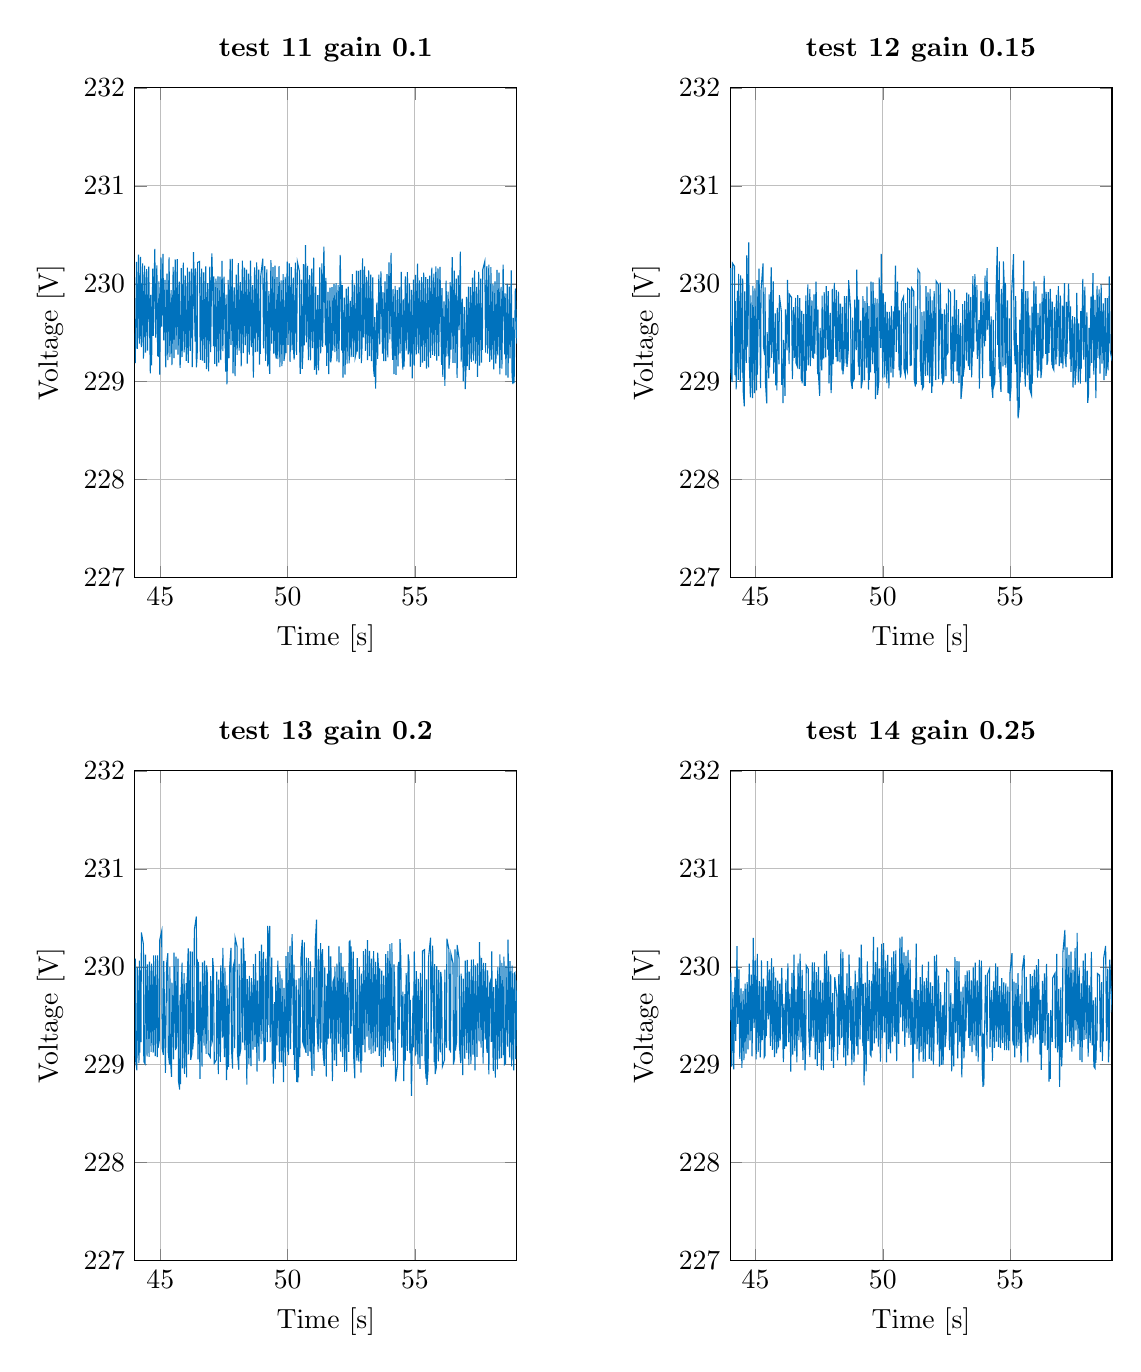
\begin{tikzpicture}

\begin{axis}[%
width=0.4\textwidth,
height=2.449in,
at={(1.024in,4.208in)},
scale only axis,
xmin=44,
xmax=59,
xlabel={Time [s]},
xmajorgrids,
ymin=227,
ymax=232,
ylabel={Voltage [V]},
ymajorgrids,
axis background/.style={fill=white},
title style={font=\bfseries},
title={test 11 gain 0.1}
]
\addplot [color=mycolor1,solid,forget plot]
  table[row sep=crcr]{%
44	229.492770060038\\
44.016	229.189241299963\\
44.064	230.223815175139\\
44.096	229.336876936412\\
44.144	230.298263495336\\
44.176	229.388760441323\\
44.224	230.275101290364\\
44.24	229.458837143648\\
44.256	229.353986510863\\
44.304	230.208444228105\\
44.336	229.235706303015\\
44.384	230.184599771871\\
44.416	229.297152922882\\
44.464	230.149300889817\\
44.496	229.317084384093\\
44.544	230.175486083347\\
44.608	229.084434787964\\
44.624	229.887563514062\\
44.656	229.167045527935\\
44.704	230.155483962333\\
44.72	229.468778712183\\
44.784	230.355745286841\\
44.816	229.449932919869\\
44.864	230.188884951321\\
44.896	229.266822937286\\
44.928	229.260919397699\\
44.944	230.023646818976\\
44.976	229.072925879563\\
45.024	230.270484987396\\
45.056	229.562056980723\\
45.104	230.305607034308\\
45.136	229.423252600066\\
45.184	230.038757852322\\
45.2	229.321021517824\\
45.216	229.147798145665\\
45.232	229.534295842035\\
45.264	230.104691528555\\
45.296	229.221596717784\\
45.344	230.270412980783\\
45.376	229.252101369577\\
45.424	229.934761324547\\
45.456	229.17021815031\\
45.504	230.172653686588\\
45.536	229.242059514996\\
45.584	230.25037668711\\
45.616	229.328745870502\\
45.664	230.251488416548\\
45.696	229.275982907747\\
45.744	230.021873855018\\
45.776	229.14068661265\\
45.808	229.368734790545\\
45.824	230.160643437315\\
45.856	229.254353023638\\
45.904	230.217027040456\\
45.936	229.298918829823\\
45.984	230.082340697135\\
46.016	229.212274751168\\
46.048	229.428379885979\\
46.064	230.16622918728\\
46.096	229.192602064824\\
46.144	230.124699193704\\
46.176	229.315002589869\\
46.224	230.154268136613\\
46.256	229.14921596219\\
46.304	230.323372366295\\
46.368	229.408544507898\\
46.384	230.156186577525\\
46.416	229.145939859769\\
46.448	229.268786799483\\
46.464	230.217413206932\\
46.544	230.228084982967\\
46.56	229.46545383171\\
46.576	229.222794353616\\
46.624	230.155351614423\\
46.656	229.216587440973\\
46.704	230.11623709429\\
46.736	229.193939394751\\
46.784	230.178274977992\\
46.816	229.129139895315\\
46.832	229.491431826549\\
46.864	230.006521202293\\
46.896	229.105053245663\\
46.944	230.175871035735\\
46.976	229.302087207162\\
47.024	230.311459678522\\
47.072	229.819878643113\\
47.088	229.36387661334\\
47.104	230.075564895499\\
47.136	229.181715642561\\
47.184	230.052593780407\\
47.216	229.155925055888\\
47.264	230.074806719844\\
47.296	229.196235813497\\
47.344	230.072312484929\\
47.376	229.219638776615\\
47.424	230.234432117089\\
47.456	229.313151808846\\
47.504	230.073882077\\
47.568	229.102679011844\\
47.584	229.889898111564\\
47.616	228.97451341693\\
47.648	229.375399775326\\
47.664	230.039740414146\\
47.696	229.241970917515\\
47.744	230.254646497343\\
47.776	229.377266367256\\
47.824	230.253575906816\\
47.856	229.086688196628\\
47.904	229.963685904731\\
47.936	229.056553779643\\
47.984	230.09277167031\\
48.016	229.27480473835\\
48.064	230.20994665425\\
48.096	229.318071872978\\
48.144	230.017816569947\\
48.176	229.155943597196\\
48.224	230.235579941629\\
48.256	229.292508955306\\
48.304	230.165559161611\\
48.336	229.373442629392\\
48.384	230.144527671348\\
48.416	229.185835941896\\
48.464	230.103811432459\\
48.496	229.27624448599\\
48.544	230.236870150585\\
48.576	229.354383751182\\
48.624	229.986372822591\\
48.64	229.303637508695\\
48.656	229.041516739596\\
48.672	229.586620728104\\
48.704	230.166651818387\\
48.736	229.301242253124\\
48.784	230.217935677396\\
48.816	229.307731165835\\
48.864	230.143563814921\\
48.896	229.175954841199\\
48.912	229.477948867283\\
48.928	229.284126206214\\
48.944	230.077493393443\\
49.024	230.255564947807\\
49.056	229.340456634837\\
49.104	230.180218965487\\
49.136	229.213014586926\\
49.184	230.14613703871\\
49.216	229.157214688587\\
49.264	229.92610176551\\
49.28	229.171802681952\\
49.296	229.081314999036\\
49.344	230.241362991942\\
49.376	229.389705733176\\
49.424	230.169609336982\\
49.456	229.287933893061\\
49.504	230.185419693785\\
49.52	229.306312941405\\
49.552	229.236619826122\\
49.584	230.06707166902\\
49.616	229.230281848273\\
49.664	230.180862169925\\
49.696	229.150511779479\\
49.744	230.035265329966\\
49.776	229.160537897817\\
49.824	230.098434121615\\
49.856	229.21244899143\\
49.888	229.275741773829\\
49.904	230.071373406137\\
49.936	229.291146524432\\
49.984	230.224961598414\\
50.016	229.376267195303\\
50.064	230.208717339995\\
50.096	229.202695674357\\
50.144	230.171180646766\\
50.176	229.322085485254\\
50.224	230.061618067909\\
50.24	229.29567131005\\
50.256	229.225409848373\\
50.272	229.339611548227\\
50.304	230.215479723311\\
50.352	229.274087994608\\
50.384	230.221861642837\\
50.464	230.124296392713\\
50.48	229.214530450299\\
50.496	229.079626555527\\
50.512	229.326324826844\\
50.544	230.042024455334\\
50.576	229.132477496927\\
50.608	229.347050454303\\
50.624	230.20139353217\\
50.656	229.372424227025\\
50.704	230.39444418827\\
50.736	229.400822514027\\
50.784	230.181672254652\\
50.816	229.221419434549\\
50.864	230.088235717502\\
50.896	229.219044514544\\
50.944	230.154669190505\\
50.976	229.342288228782\\
51.024	230.266302919242\\
51.056	229.120912937457\\
51.088	229.19419275077\\
51.104	229.972118642039\\
51.136	229.071668187226\\
51.184	229.883642826459\\
51.216	229.11544020471\\
51.264	230.166712463413\\
51.296	229.289112711744\\
51.328	229.476861346648\\
51.344	230.207659323239\\
51.376	229.357069014775\\
51.424	230.380086788062\\
51.488	229.370701876316\\
51.504	230.059340574872\\
51.536	229.161691756842\\
51.584	229.917040324282\\
51.616	229.079092112704\\
51.664	229.960252879131\\
51.696	229.198853115963\\
51.728	229.284681511972\\
51.744	229.964840198977\\
51.776	229.318308104808\\
51.824	229.999125396168\\
51.856	229.303213357965\\
51.904	230.007945388318\\
51.936	229.208422819723\\
51.984	229.986483130755\\
52.016	229.196871778447\\
52.064	230.293818785734\\
52.112	229.670355469469\\
52.128	229.319051809922\\
52.144	229.98560337592\\
52.176	229.041744618653\\
52.224	229.857497217281\\
52.256	229.072235101164\\
52.304	229.95148969349\\
52.336	229.185651624899\\
52.352	229.683558618216\\
52.384	229.971021130773\\
52.416	229.186953611068\\
52.464	229.826360490591\\
52.496	229.250932926513\\
52.544	230.097903701299\\
52.576	229.254634150208\\
52.624	229.991948142013\\
52.656	229.251224072239\\
52.688	229.292855239749\\
52.704	230.135215398847\\
52.736	229.308351794928\\
52.784	230.131369476862\\
52.816	229.232620065995\\
52.864	230.141633889147\\
52.896	229.189764194559\\
52.928	229.393754993248\\
52.944	230.259285158907\\
52.976	229.454164668639\\
53.024	230.178260334608\\
53.056	229.31561549611\\
53.104	230.071327492134\\
53.136	229.22151085666\\
53.184	230.137295094505\\
53.216	229.260639504585\\
53.264	230.092238540856\\
53.296	229.210606178038\\
53.344	230.064965702144\\
53.376	229.1272763118\\
53.408	229.049560752731\\
53.424	229.658975507958\\
53.456	228.928633528621\\
53.504	229.807146426834\\
53.536	229.232874581904\\
53.584	230.09366986254\\
53.616	229.380710684851\\
53.664	230.126010840177\\
53.728	229.287574920897\\
53.744	229.913591229421\\
53.776	229.211108813779\\
53.824	230.02507165048\\
53.856	229.210617535234\\
53.904	230.097404006752\\
53.936	229.247954415592\\
53.952	229.77869812253\\
53.984	230.217867310344\\
54.016	229.431500303556\\
54.064	230.316367699669\\
54.096	229.453961136421\\
54.128	229.222494769944\\
54.144	229.945754022851\\
54.176	229.077569460977\\
54.224	229.977615942716\\
54.256	229.069825010654\\
54.304	229.936416079668\\
54.336	229.155820793634\\
54.384	229.963562455585\\
54.416	229.288479845825\\
54.464	230.121000961945\\
54.496	229.27851151689\\
54.528	229.124149417852\\
54.544	229.839840587217\\
54.576	229.154238927605\\
54.624	230.076780866064\\
54.656	229.317531550718\\
54.704	230.119053578281\\
54.736	229.280447297418\\
54.768	229.329108675005\\
54.784	230.003395965444\\
54.816	229.155647471228\\
54.864	229.937931631248\\
54.896	229.034879633446\\
54.944	230.043517618471\\
54.976	229.163412433623\\
55.024	230.091435505853\\
55.056	229.279270376942\\
55.104	230.206184161753\\
55.136	229.289018924605\\
55.184	230.033687823036\\
55.216	229.152317834372\\
55.264	230.068691004628\\
55.296	229.196527193974\\
55.344	230.114477568737\\
55.376	229.213401733336\\
55.424	230.067339576411\\
55.456	229.134389099864\\
55.504	230.046644360925\\
55.536	229.147804883004\\
55.552	229.653697674461\\
55.584	230.08415859642\\
55.616	229.244648630901\\
55.664	230.163983571317\\
55.696	229.274134458717\\
55.744	230.10395160591\\
55.776	229.264279520513\\
55.792	229.667328234934\\
55.824	230.178451372407\\
55.856	229.2159927152\\
55.904	230.157855944691\\
55.936	229.261009607078\\
55.984	230.172703514677\\
56.048	229.17279577187\\
56.064	229.956480035639\\
56.096	229.04894591641\\
56.144	229.819856841249\\
56.176	228.957294960199\\
56.224	230.032039033728\\
56.256	229.259708153228\\
56.304	229.919580433441\\
56.336	229.133801329679\\
56.368	229.244501520443\\
56.384	230.015897165264\\
56.416	229.328675534801\\
56.464	230.27218295132\\
56.496	229.191925928532\\
56.544	230.133876351786\\
56.576	229.191463605319\\
56.624	230.052674709106\\
56.656	229.040856734792\\
56.704	230.085113606264\\
56.736	229.526208323734\\
56.784	230.328956728434\\
56.816	229.205064767816\\
56.864	229.848908527203\\
56.896	229.003284731725\\
56.944	229.761535845869\\
56.976	228.924593476715\\
57.008	229.145378213689\\
57.024	229.865467342259\\
57.056	229.158889527599\\
57.104	229.971853616809\\
57.136	229.121337694607\\
57.184	229.965211198118\\
57.216	229.202407305738\\
57.264	230.062459638346\\
57.296	229.215791432143\\
57.344	230.137196789784\\
57.376	229.184251472258\\
57.392	229.505758435782\\
57.424	229.969541300831\\
57.456	229.050454962561\\
57.504	230.121678429842\\
57.536	229.164713462223\\
57.584	230.051613805559\\
57.616	229.194812610805\\
57.632	229.651310569568\\
57.648	229.324465473951\\
57.664	230.143026884443\\
57.744	230.226474947225\\
57.776	229.298417490128\\
57.824	230.179650085004\\
57.856	229.28793246208\\
57.904	230.195887507874\\
57.936	229.203853132115\\
57.968	229.389726416053\\
57.984	230.170592538441\\
58.016	229.226549249134\\
58.064	229.998541477802\\
58.096	229.127637488147\\
58.144	230.023915021787\\
58.176	229.186404735065\\
58.208	229.436758396594\\
58.224	230.141399397618\\
58.256	229.268517029605\\
58.304	230.113545914312\\
58.336	229.074735169688\\
58.384	229.968168545259\\
58.416	229.133094852438\\
58.464	230.196258779991\\
58.528	229.279094600755\\
58.544	229.901586120548\\
58.576	229.064372308446\\
58.624	230.00041198154\\
58.656	229.0424968711\\
58.704	229.969870564833\\
58.736	229.239244477146\\
58.784	230.136197619435\\
58.816	229.060091860968\\
58.848	228.976427725103\\
58.864	229.651343173361\\
58.896	228.985380879921\\
58.944	229.951771114889\\
59.008	229.389871003751\\
};
\end{axis}

\begin{axis}[%
width=0.4\textwidth,
height=2.449in,
at={(4in,4.208in)},
scale only axis,
xmin=44,
xmax=59,
xlabel={Time [s]},
xmajorgrids,
ymin=227,
ymax=232,
ylabel={Voltage [V]},
ymajorgrids,
axis background/.style={fill=white},
title style={font=\bfseries},
title={test 12  gain 0.15}
]
\addplot [color=mycolor1,solid,forget plot]
  table[row sep=crcr]{%
44	229.130235676761\\
44.016	230.159685836235\\
44.032	229.107005301554\\
44.08	228.996793231795\\
44.096	230.209561886556\\
44.176	230.177596790432\\
44.192	229.068363667576\\
44.208	229.823855371043\\
44.24	228.922180968514\\
44.288	229.92866796982\\
44.32	229.018101086993\\
44.336	230.101498888287\\
44.4	228.999618966926\\
44.416	230.086462885656\\
44.48	229.092090106973\\
44.496	230.052868944338\\
44.512	228.916866889458\\
44.56	228.748848098607\\
44.576	229.921847190406\\
44.64	229.192905483871\\
44.656	230.290383335923\\
44.672	229.353500193857\\
44.736	230.42358063291\\
44.752	229.221782447005\\
44.8	228.840795776687\\
44.816	229.882152437058\\
44.88	228.832911371559\\
44.896	229.977720581823\\
44.96	228.882940675658\\
44.976	229.952561342634\\
45.04	228.911662986403\\
45.056	230.037327764981\\
45.072	229.07377752523\\
45.136	230.154239384828\\
45.2	228.934791664889\\
45.216	229.932338843975\\
45.296	230.207071982596\\
45.312	229.361470019814\\
45.36	229.273174355321\\
45.376	229.964205008424\\
45.392	228.985307715041\\
45.44	228.778791881322\\
45.456	229.505773762435\\
45.52	229.033380594894\\
45.536	229.89109894229\\
45.552	229.14554834704\\
45.616	230.167047346538\\
45.632	229.243512735809\\
45.696	230.025390016507\\
45.712	229.082379682454\\
45.776	229.696720589593\\
45.792	228.961985933934\\
45.824	229.331216248935\\
45.84	228.910964659425\\
45.856	229.754789187809\\
45.92	229.176592653188\\
45.936	229.883540205014\\
46.016	229.714355943039\\
46.032	228.968456906241\\
46.064	229.185987985435\\
46.08	228.782923210271\\
46.096	229.427290747266\\
46.16	228.854877805602\\
46.176	229.73806657602\\
46.24	229.320126481281\\
46.256	230.04071248684\\
46.32	229.179012887001\\
46.336	229.890446818918\\
46.416	229.86046752663\\
46.448	229.026568868343\\
46.496	229.76057300938\\
46.528	229.244217897335\\
46.576	229.855393827091\\
46.592	229.190856295809\\
46.64	229.158125707713\\
46.656	229.885400923282\\
46.72	229.127933177271\\
46.736	229.854340973873\\
46.8	229.00838478157\\
46.816	229.722612933624\\
46.832	228.983905293137\\
46.896	229.693532520517\\
46.912	228.964808337034\\
46.96	228.964644273351\\
46.976	229.882891182496\\
46.992	229.113679626394\\
47.056	229.994440080097\\
47.072	229.166231851734\\
47.136	229.946213338014\\
47.152	229.160092219967\\
47.216	229.830780215805\\
47.232	229.252803539926\\
47.28	229.243200070435\\
47.296	229.890912014799\\
47.328	229.286825908345\\
47.376	230.0209655175\\
47.44	229.078778861296\\
47.456	229.735066043178\\
47.472	229.07717552196\\
47.52	228.854857815804\\
47.536	229.549093202308\\
47.6	229.116935190141\\
47.616	229.87815469919\\
47.632	229.227008146085\\
47.664	229.531952917368\\
47.68	229.237811221094\\
47.696	229.913780431769\\
47.76	229.248744011342\\
47.776	229.977105018184\\
47.84	229.324999800983\\
47.856	229.924189821177\\
47.888	228.983433126087\\
47.936	229.702250040297\\
47.968	228.88415845159\\
48	229.121524321902\\
48.016	229.948361842808\\
48.048	229.179580098836\\
48.096	230.008580123947\\
48.16	229.252995669826\\
48.176	229.935107834276\\
48.208	229.212673389973\\
48.24	229.214473046081\\
48.256	229.9196642806\\
48.32	229.197845245852\\
48.336	229.798186799922\\
48.4	229.113664447086\\
48.416	229.765500879884\\
48.432	229.074442320175\\
48.48	229.210816938098\\
48.496	229.872802367735\\
48.56	229.187169553038\\
48.576	229.874067088603\\
48.592	229.151060557666\\
48.64	229.312013179355\\
48.656	230.036183830807\\
48.736	229.731856702731\\
48.752	229.008169852951\\
48.8	228.926494618283\\
48.816	229.654019379548\\
48.832	229.006238582495\\
48.88	229.031395249553\\
48.896	229.839351464854\\
48.96	229.322154474392\\
48.976	230.143605876566\\
49.04	229.154715813012\\
49.056	229.837302002415\\
49.072	229.068637305645\\
49.136	229.625529296058\\
49.152	228.933075731774\\
49.2	229.020175585856\\
49.216	229.873124930953\\
49.264	229.438100678474\\
49.28	229.012868815129\\
49.296	229.822112607851\\
49.36	229.143663432575\\
49.376	229.972276526128\\
49.44	228.920537154225\\
49.456	229.771065325362\\
49.472	229.020389585153\\
49.488	229.472857131819\\
49.52	229.095793106215\\
49.536	230.021299664988\\
49.6	229.179314670192\\
49.616	230.013400359712\\
49.68	229.08818351574\\
49.696	229.85514260452\\
49.712	228.822629338994\\
49.776	229.846217211563\\
49.792	228.867278776938\\
49.84	228.996320538689\\
49.856	230.064124531875\\
49.92	229.346905861839\\
49.936	230.30554495019\\
50	229.035498919651\\
50.016	229.90230609382\\
50.08	229.045691585444\\
50.096	229.815375522127\\
50.16	228.984881769488\\
50.176	229.713913949578\\
50.24	228.933169432014\\
50.256	229.712992990583\\
50.32	229.092039120362\\
50.336	229.775508924284\\
50.4	229.045649101725\\
50.416	229.719566986083\\
50.432	229.132003379064\\
50.496	230.184834341024\\
50.528	229.305095335098\\
50.576	230.021904019696\\
50.64	229.116625014434\\
50.656	229.72825437204\\
50.688	229.043349652658\\
50.72	229.089732223987\\
50.736	229.815085286882\\
50.816	229.869831298058\\
50.832	229.131722148621\\
50.88	229.070671722379\\
50.896	229.802430182125\\
50.912	229.159200447022\\
50.96	229.110564586356\\
50.976	229.953481450808\\
51.056	229.93849186272\\
51.072	229.160795824312\\
51.088	229.593695929752\\
51.12	229.165942140896\\
51.136	229.957684419465\\
51.216	229.923270911616\\
51.232	229.023681967414\\
51.28	228.951431434454\\
51.296	229.773510597639\\
51.312	228.973443935466\\
51.344	229.576038196166\\
51.36	229.333424034232\\
51.376	230.145895102617\\
51.456	230.108851802393\\
51.472	229.203010098735\\
51.52	228.969035028893\\
51.536	229.709578111701\\
51.552	228.925976011372\\
51.6	228.951264212751\\
51.616	229.717655194904\\
51.68	229.061278878026\\
51.696	229.977171369117\\
51.76	229.0654880978\\
51.776	229.912494107041\\
51.84	228.986879484474\\
51.856	229.948606599918\\
51.92	228.886969182476\\
51.936	229.829476072078\\
51.952	228.953555327333\\
52.016	229.926209382436\\
52.08	229.01541112936\\
52.096	230.026588065765\\
52.176	229.992910480729\\
52.192	229.026870550335\\
52.256	230.011877195264\\
52.32	229.032911340673\\
52.336	229.691913616124\\
52.352	228.989379558519\\
52.4	229.016790152713\\
52.416	229.739891237378\\
52.48	229.058436024462\\
52.496	229.800114030269\\
52.512	229.276337022803\\
52.56	229.299077897257\\
52.576	229.940347078888\\
52.656	229.912124663122\\
52.672	229.252861241662\\
52.688	229.006233452567\\
52.736	229.663533476056\\
52.768	228.981075696275\\
52.816	229.941749395979\\
52.832	229.204413833121\\
52.896	229.833301522974\\
52.912	229.107056853268\\
52.944	229.485796615307\\
52.96	229.065126250614\\
52.976	229.742443198938\\
52.992	228.989727000254\\
53.056	229.600319996116\\
53.072	228.824276606301\\
53.12	228.968625329804\\
53.136	229.793228934665\\
53.152	229.051486079814\\
53.2	229.148297341752\\
53.216	229.825137145667\\
53.28	229.215319095049\\
53.296	229.909912357212\\
53.36	229.158869203812\\
53.376	229.891571347795\\
53.408	229.122060669841\\
53.456	229.86552851822\\
53.488	229.044817582693\\
53.52	229.337478184486\\
53.536	230.078645518102\\
53.568	229.308439866862\\
53.616	230.098766777165\\
53.68	229.411231237014\\
53.696	229.985669448599\\
53.712	229.232465163796\\
53.776	229.630080592296\\
53.792	228.930300141759\\
53.856	229.92861931633\\
53.92	229.037816022476\\
53.936	229.852168190137\\
54	229.362340327315\\
54.016	230.082069528199\\
54.032	229.417967914248\\
54.096	230.159232960406\\
54.112	229.533053119267\\
54.176	229.896827480808\\
54.208	229.056564396853\\
54.256	229.668082201609\\
54.272	228.975067055733\\
54.32	228.836448041328\\
54.336	229.632093772717\\
54.352	228.946168834497\\
54.4	228.992646736172\\
54.448	229.902210407433\\
54.496	230.375491158536\\
54.512	229.375307240812\\
54.528	230.03657573375\\
54.56	229.127281877173\\
54.576	230.227724923935\\
54.592	229.100981584585\\
54.64	228.896351611161\\
54.656	229.948314814578\\
54.72	229.157923636824\\
54.736	230.229494497028\\
54.768	229.993036812109\\
54.8	229.172196702526\\
54.816	230.0094522725\\
54.832	229.143093785081\\
54.896	229.830996521196\\
54.912	228.892884362821\\
54.96	228.884979924619\\
54.976	229.647741990779\\
54.992	228.801871988209\\
55.04	228.960150515912\\
55.056	229.879955279335\\
55.136	230.302517434702\\
55.152	229.437669447539\\
55.2	229.17835587955\\
55.216	229.874562205096\\
55.28	228.806121720462\\
55.296	229.374960309339\\
55.312	228.627170148835\\
55.36	228.745060309146\\
55.376	229.633501870608\\
55.392	228.990892380607\\
55.456	229.946686966347\\
55.472	229.097071792147\\
55.536	230.237521377886\\
55.552	229.228563163178\\
55.6	228.95155748075\\
55.616	229.925457269603\\
55.68	229.06611764337\\
55.696	229.92499639213\\
55.76	228.920061076052\\
55.776	229.676844631431\\
55.792	228.904557936402\\
55.84	228.863370293741\\
55.856	229.76574809317\\
55.872	228.981545172235\\
55.936	230.024682618513\\
55.952	229.315888320528\\
56.016	229.972275425452\\
56.048	229.26787701302\\
56.08	229.041719267676\\
56.096	229.702612024646\\
56.128	229.113728889079\\
56.176	229.798891726175\\
56.208	229.037546606369\\
56.24	229.117340824778\\
56.256	229.898889597938\\
56.288	229.237904003318\\
56.336	230.081923922438\\
56.384	229.564244050015\\
56.4	229.284218409271\\
56.416	229.917090307221\\
56.448	229.172997256044\\
56.48	229.216928281982\\
56.496	229.915610393991\\
56.528	229.294669112628\\
56.576	229.947725309463\\
56.64	229.170509939121\\
56.656	229.818432767565\\
56.672	229.145083736922\\
56.72	229.117930155469\\
56.736	229.762758149696\\
56.8	229.17697617354\\
56.816	229.887336974886\\
56.832	229.255322606217\\
56.896	229.97507166207\\
56.928	229.160755604204\\
56.976	229.879768128403\\
56.992	229.196027240139\\
57.04	229.193439476261\\
57.056	229.777125099393\\
57.072	229.135696400877\\
57.136	230.00684069916\\
57.152	229.278842767269\\
57.2	229.149763142942\\
57.216	229.815288677706\\
57.232	229.281926165573\\
57.296	230.001665513125\\
57.36	229.230642809904\\
57.376	229.770079298924\\
57.392	229.10097481988\\
57.456	229.668563305485\\
57.472	228.940109199201\\
57.536	229.660710097928\\
57.552	228.967153934957\\
57.6	229.155632348433\\
57.616	229.907562885994\\
57.68	228.994878819618\\
57.696	229.594635138764\\
57.76	228.980135277487\\
57.776	229.72130537091\\
57.792	229.133163581753\\
57.856	230.049360307486\\
57.888	229.225912896935\\
57.936	229.971325694563\\
57.968	228.995498780016\\
57.984	229.394784052091\\
58.016	229.707259181789\\
58.048	228.78487587817\\
58.08	228.878354830839\\
58.096	229.55048118986\\
58.128	229.037349420866\\
58.176	229.86993655767\\
58.208	229.192534692379\\
58.224	229.729591676563\\
58.256	230.107766049843\\
58.288	229.073673861845\\
58.336	229.836986889118\\
58.368	228.832310029033\\
58.416	229.977969973517\\
58.448	229.242905414067\\
58.496	229.941924102087\\
58.528	229.082805879596\\
58.576	229.990610896586\\
58.608	229.184236288484\\
58.656	229.801063518386\\
58.688	229.015627042545\\
58.736	229.852880561568\\
58.768	229.060870937043\\
58.8	229.207449609156\\
58.816	229.853502266124\\
58.848	229.116749977112\\
58.896	230.076442940127\\
58.928	229.318702071834\\
59.008	229.210615056122\\
};
\end{axis}

\begin{axis}[%
width=0.4\textwidth,
height=2.449in,
at={(1.024in,0.793in)},
scale only axis,
xmin=44,
xmax=59,
xlabel={Time [s]},
xmajorgrids,
ymin=227,
ymax=232,
ylabel={Voltage [V]},
ymajorgrids,
axis background/.style={fill=white},
title style={font=\bfseries},
title={test 13  gain 0.2}
]
\addplot [color=mycolor1,solid,forget plot]
  table[row sep=crcr]{%
44	229.09084912557\\
44.016	230.08421256301\\
44.032	229.040600188628\\
44.08	228.942584281533\\
44.096	229.994807573955\\
44.16	229.016848767733\\
44.176	230.063726654324\\
44.192	229.124488265565\\
44.208	229.964201238551\\
44.24	229.2309066284\\
44.256	230.350022029947\\
44.336	230.231187816979\\
44.352	229.031578642569\\
44.4	229.010386110512\\
44.416	230.123215500702\\
44.48	229.085123311429\\
44.496	230.023725680729\\
44.56	229.080800171548\\
44.576	230.053856538689\\
44.64	229.132329939267\\
44.656	230.032625188527\\
44.72	229.123574497975\\
44.736	230.117475627316\\
44.8	229.088292847707\\
44.816	230.11755265795\\
44.88	229.079129476238\\
44.896	230.117541870502\\
44.912	229.170613109942\\
44.96	229.251106875413\\
44.976	230.272922195102\\
45.056	230.36694281027\\
45.072	229.169535197941\\
45.12	229.100724206415\\
45.136	230.060626098434\\
45.2	228.916881084634\\
45.248	230.031013419566\\
45.296	230.13855969867\\
45.312	229.125965987976\\
45.36	229.00244561221\\
45.376	229.99687946526\\
45.392	229.080662810492\\
45.44	228.876537144553\\
45.456	229.838026529078\\
45.52	229.054218896754\\
45.536	230.14527753053\\
45.6	229.148938669321\\
45.616	230.104663716259\\
45.632	229.164125141614\\
45.696	230.083307150663\\
45.712	228.834390646752\\
45.76	228.747224721658\\
45.776	229.713527959044\\
45.792	228.802824478173\\
45.808	229.663673706163\\
45.856	230.042713540309\\
45.872	228.962388592311\\
45.936	229.934325601032\\
45.952	228.906266963595\\
46.016	229.834304890573\\
46.032	228.870925262291\\
46.048	229.801620363687\\
46.096	230.188022752848\\
46.112	229.106833196985\\
46.176	230.156728366675\\
46.192	229.049894190046\\
46.24	229.114229468231\\
46.256	230.153680903116\\
46.272	229.157088663503\\
46.32	229.313782648534\\
46.336	230.376488373878\\
46.416	230.512892340339\\
46.432	229.327597990403\\
46.448	230.08168624529\\
46.48	229.055698910259\\
46.496	230.051307165928\\
46.56	228.855086831751\\
46.576	229.849188719085\\
46.64	228.981622000906\\
46.656	230.0454781781\\
46.72	229.194942223279\\
46.736	230.061888819443\\
46.8	229.110566099274\\
46.816	230.015171301604\\
46.848	229.922658306448\\
46.88	229.116397726135\\
46.96	229.079235216205\\
46.976	229.903588737282\\
47.024	229.222124859863\\
47.04	229.238090786569\\
47.056	230.089356006955\\
47.088	229.978680579654\\
47.12	229.013565505189\\
47.2	229.049668949623\\
47.216	229.949380282915\\
47.264	229.17086110765\\
47.28	228.904365792668\\
47.296	229.869429918831\\
47.36	229.028813435235\\
47.376	230.014798104036\\
47.44	229.277977514983\\
47.456	230.192896760168\\
47.504	229.277617298368\\
47.52	229.076747169896\\
47.536	229.991549197784\\
47.6	228.843042669735\\
47.616	229.811171824417\\
47.632	228.949761583691\\
47.648	229.676115174387\\
47.68	228.979044068461\\
47.728	230.010419282176\\
47.776	230.192783322377\\
47.792	229.178764641076\\
47.84	228.959989198456\\
47.856	229.98908609034\\
47.888	230.028743974595\\
47.92	229.16957508257\\
47.936	230.297372687759\\
48.016	230.2042296376\\
48.032	229.118437690911\\
48.08	228.949309316943\\
48.096	230.029669820091\\
48.112	229.088381625643\\
48.16	229.162462838207\\
48.176	230.187092953777\\
48.24	229.226487541079\\
48.256	230.298188199444\\
48.288	230.113176452387\\
48.32	229.148404509201\\
48.336	230.060659676416\\
48.4	228.798107974323\\
48.416	229.8728957881\\
48.48	229.008162687965\\
48.496	229.907744392408\\
48.56	228.985467338305\\
48.576	229.884663340963\\
48.64	229.154012078505\\
48.656	230.027595451336\\
48.72	229.183496928529\\
48.736	230.130869560578\\
48.8	228.929312944532\\
48.816	229.859953103817\\
48.88	229.036161512225\\
48.896	230.159395022522\\
48.96	229.210353792445\\
48.976	230.225278750488\\
49.04	229.239250154639\\
49.056	230.152609798014\\
49.072	229.036262163715\\
49.12	229.051558126506\\
49.136	230.084316719243\\
49.2	229.230998444376\\
49.216	230.418861990597\\
49.232	229.404216776184\\
49.248	230.271588645468\\
49.296	230.416255975506\\
49.312	229.230123974959\\
49.376	230.092524193509\\
49.392	229.011315531418\\
49.408	229.798211171677\\
49.44	228.807104110164\\
49.488	229.639526685919\\
49.52	228.954704813321\\
49.536	229.894871555143\\
49.584	229.197728603938\\
49.616	230.062316294523\\
49.68	229.025007028482\\
49.696	229.958304102495\\
49.76	229.023738052337\\
49.776	229.88243533988\\
49.84	228.823800160107\\
49.856	229.785486068068\\
49.92	228.989678950161\\
49.936	230.107623994266\\
50	229.134155069724\\
50.016	230.150036901442\\
50.032	229.097641023246\\
50.096	230.213052419169\\
50.112	229.160438679629\\
50.176	230.332407353159\\
50.24	229.100109925602\\
50.256	230.022096587832\\
50.272	228.948068629219\\
50.336	229.865393692355\\
50.352	228.829632135832\\
50.4	228.826224147973\\
50.416	229.766214622795\\
50.432	228.870299267638\\
50.448	229.882225435074\\
50.48	229.081201272717\\
50.528	230.111803439885\\
50.576	230.274848609033\\
50.592	229.235641796402\\
50.64	229.193689530052\\
50.656	230.248105285904\\
50.672	229.221404940751\\
50.72	229.120795535521\\
50.736	230.09361825936\\
50.8	229.089753641438\\
50.816	230.088003222098\\
50.88	229.135365318411\\
50.896	230.055049531776\\
50.912	229.178635293936\\
50.96	228.887615840231\\
50.976	229.893147974815\\
51.04	228.93724051142\\
51.056	229.986952436132\\
51.072	229.432680972363\\
51.088	230.247789466377\\
51.136	230.480306397812\\
51.152	229.401503263513\\
51.2	229.129554088654\\
51.216	230.182068722691\\
51.28	229.164142400109\\
51.296	230.240849805981\\
51.312	229.225811081057\\
51.328	230.080738986837\\
51.376	230.179912101844\\
51.392	229.126266716306\\
51.44	228.988347054805\\
51.456	229.992728215825\\
51.52	228.878200639649\\
51.536	229.805918422419\\
51.552	229.208200198819\\
51.568	229.931338142124\\
51.6	229.266723582403\\
51.616	230.212303184875\\
51.68	229.266795993707\\
51.696	230.105099013673\\
51.76	228.832175468891\\
51.776	229.840010192044\\
51.808	229.866419888726\\
51.84	229.044570183093\\
51.856	229.995281080211\\
51.92	228.987965636305\\
51.936	230.031584708688\\
52	229.21545707846\\
52.016	230.207938495726\\
52.08	229.134901429987\\
52.096	230.141679892402\\
52.16	229.07959177433\\
52.176	229.99761367489\\
52.24	228.928174680756\\
52.256	229.954584877236\\
52.32	228.928741625839\\
52.336	229.83725648009\\
52.4	229.130784708489\\
52.416	230.253217833965\\
52.448	230.263323942589\\
52.48	229.317269176111\\
52.496	230.208527056094\\
52.512	229.393335735929\\
52.576	230.154362120488\\
52.592	229.094719496548\\
52.64	228.861748284896\\
52.656	229.873348129143\\
52.72	229.040974717262\\
52.736	230.089652091057\\
52.752	229.174125886859\\
52.8	229.031407533749\\
52.816	229.997145266264\\
52.88	228.919035392143\\
52.896	229.929528445102\\
52.912	229.038422583882\\
52.928	229.82796903473\\
52.96	229.201749752409\\
52.976	230.158780258902\\
53.04	229.12632025939\\
53.056	230.181573809253\\
53.12	229.287010346804\\
53.136	230.271660831632\\
53.2	229.149013773144\\
53.216	230.161448407405\\
53.28	229.110141353595\\
53.296	230.084390607622\\
53.36	229.119828758078\\
53.376	230.159853090045\\
53.44	229.137537095374\\
53.456	230.049559751718\\
53.52	229.177504461581\\
53.536	230.143696225781\\
53.568	229.991009200943\\
53.6	229.091599531883\\
53.616	229.983133517995\\
53.68	228.97650334669\\
53.696	229.959604897669\\
53.76	228.98212367841\\
53.776	229.909067656159\\
53.84	229.077061810726\\
53.856	230.128149361815\\
53.92	229.167909496353\\
53.936	230.158932841552\\
54	229.145230495424\\
54.016	230.231793572317\\
54.08	229.23631113896\\
54.096	230.241439114891\\
54.112	229.344327183214\\
54.16	229.040643407334\\
54.176	230.025269110823\\
54.208	229.78109756819\\
54.24	228.829185287186\\
54.32	229.007121759766\\
54.336	230.000981363644\\
54.368	230.050424595292\\
54.384	229.357765124556\\
54.416	230.281892790554\\
54.448	230.075263313627\\
54.48	229.173843715861\\
54.528	229.745402356703\\
54.56	228.832759069119\\
54.608	229.720316433237\\
54.624	229.041222860474\\
54.656	229.934173114395\\
54.704	229.140818772082\\
54.736	230.125584218464\\
54.768	230.050913844761\\
54.8	229.119672647822\\
54.816	229.66223363387\\
54.864	228.681797732342\\
54.928	229.704343530334\\
54.944	229.176142685487\\
54.976	230.156694098749\\
55.024	229.107422582117\\
55.04	229.116808396781\\
55.056	229.956028703078\\
55.12	229.006154823784\\
55.136	229.876070032119\\
55.2	228.957133723242\\
55.216	229.938732491885\\
55.28	229.088332888157\\
55.296	230.160010520809\\
55.376	230.174185700622\\
55.392	229.064422030338\\
55.44	228.856241780086\\
55.456	229.872484856511\\
55.472	228.794366368355\\
55.52	228.959427351032\\
55.536	230.093533459263\\
55.616	230.297997218446\\
55.632	229.219507063233\\
55.696	230.216485465899\\
55.76	229.027736827741\\
55.776	230.027556736467\\
55.792	228.905023894916\\
55.84	228.96949313546\\
55.856	230.006404867837\\
55.92	229.034602658653\\
55.936	229.966796250321\\
55.984	229.163589098458\\
56	229.126542831133\\
56.016	229.947183503691\\
56.048	229.852917476065\\
56.08	228.982950799928\\
56.16	229.047910031936\\
56.176	229.97216788904\\
56.192	229.34654879952\\
56.24	229.173764557885\\
56.256	230.286880364489\\
56.336	230.176331318354\\
56.352	229.145959638189\\
56.368	229.927920244464\\
56.4	229.123614780389\\
56.416	230.129768605015\\
56.496	230.036392705826\\
56.512	229.001419866711\\
56.56	229.069480560784\\
56.576	230.178255135694\\
56.592	229.145770547613\\
56.64	229.242731072905\\
56.656	230.224152893191\\
56.736	230.082802224659\\
56.752	229.180661346745\\
56.8	229.016030574823\\
56.816	229.930111615269\\
56.88	228.893958526048\\
56.896	229.879370461251\\
56.96	229.059766025792\\
56.976	230.063930634361\\
57.04	229.121159178989\\
57.056	230.071221673705\\
57.12	228.995563358215\\
57.136	229.949440526985\\
57.2	229.00857047713\\
57.216	230.073758932405\\
57.28	229.103804795717\\
57.296	230.074914864247\\
57.36	228.943525249619\\
57.376	230.015119337859\\
57.44	229.080376283068\\
57.456	230.034099680213\\
57.52	229.239740255125\\
57.536	230.252756280407\\
57.6	229.17396187699\\
57.616	230.091123461972\\
57.68	229.012271984467\\
57.696	230.038795110602\\
57.76	229.256926501472\\
57.776	230.037989776714\\
57.824	229.153886673798\\
57.84	229.122684547625\\
57.856	229.963831703853\\
57.904	228.901066711854\\
57.936	229.830316710174\\
57.968	229.857175280637\\
58	229.233177185716\\
58.016	230.158199850784\\
58.064	229.131129906827\\
58.08	228.938424168885\\
58.096	229.792221525922\\
58.16	228.869730878905\\
58.176	229.879606358563\\
58.208	229.753725669863\\
58.24	228.952001753411\\
58.256	229.997824673599\\
58.32	229.061540910037\\
58.336	230.126253526023\\
58.4	229.066476919098\\
58.416	230.038778364723\\
58.48	229.10115158247\\
58.496	230.104314570988\\
58.512	229.000286466902\\
58.56	229.014287885779\\
58.576	230.00901012438\\
58.64	229.183943032826\\
58.656	230.278040312577\\
58.72	229.075802480233\\
58.736	230.057312124818\\
58.8	228.984027730708\\
58.816	230.012092578138\\
58.88	228.942532572869\\
58.896	229.928894307378\\
58.928	229.940666222033\\
58.96	229.056852190369\\
59.008	229.862034712849\\
};
\end{axis}

\begin{axis}[%
width=0.4\textwidth,
height=2.449in,
at={(4in,0.793in)},
scale only axis,
xmin=44,
xmax=59,
xlabel={Time [s]},
xmajorgrids,
ymin=227,
ymax=232,
ylabel={Voltage [V]},
ymajorgrids,
axis background/.style={fill=white},
title style={font=\bfseries},
title={test 14  gain 0.25}
]
\addplot [color=mycolor1,solid,forget plot]
  table[row sep=crcr]{%
44	229.45458576392\\
44.032	229.941397753392\\
44.064	228.981766839158\\
44.112	229.742442065137\\
44.144	228.952543061262\\
44.192	229.896472829657\\
44.224	229.243272238551\\
44.272	230.209676814381\\
44.304	229.418034236731\\
44.352	229.974002845668\\
44.368	229.350189580719\\
44.384	229.059474884474\\
44.432	229.780349199221\\
44.464	228.967658022034\\
44.512	229.751172706804\\
44.544	229.04605527614\\
44.592	229.826875130123\\
44.624	229.113054612772\\
44.64	229.372009156464\\
44.672	229.843489490793\\
44.704	229.157020058971\\
44.752	230.033333816563\\
44.784	229.247757938759\\
44.832	229.918967252939\\
44.864	229.085086249605\\
44.912	230.295967226952\\
44.944	229.376680007549\\
44.992	230.064957064794\\
45.024	229.054813545393\\
45.072	230.130916669033\\
45.104	229.131762351313\\
45.152	229.852695288207\\
45.184	229.0758544295\\
45.216	229.333344592803\\
45.232	230.065481982647\\
45.264	229.251578303238\\
45.312	229.878276499379\\
45.344	229.077571759979\\
45.376	229.095717380022\\
45.392	229.801017663244\\
45.424	229.291270376553\\
45.472	230.057397949992\\
45.504	229.463482130481\\
45.552	229.973715375572\\
45.584	229.191901593068\\
45.632	230.087107473746\\
45.664	229.15172474631\\
45.712	230.000237008653\\
45.744	229.078625950179\\
45.792	229.888945164173\\
45.824	229.117297698696\\
45.872	229.857907050795\\
45.888	229.182225005477\\
45.904	229.192064308569\\
45.952	229.82722925769\\
45.968	229.246845305044\\
46.032	229.989252874007\\
46.08	229.168467022497\\
46.096	229.026540100602\\
46.112	229.621821470854\\
46.144	229.161927969447\\
46.192	229.870298474708\\
46.208	229.188465847214\\
46.24	229.61749657868\\
46.272	230.034249246204\\
46.304	229.23018092283\\
46.352	229.726057760297\\
46.384	228.928844045724\\
46.432	229.938088326795\\
46.464	229.102279397775\\
46.48	229.514805020393\\
46.512	230.124008314467\\
46.544	229.139404034408\\
46.592	229.769222596997\\
46.624	229.023276029054\\
46.672	230.033930272614\\
46.704	229.251295638106\\
46.752	230.135025368539\\
46.784	229.228175132059\\
46.832	229.96932075845\\
46.848	229.258711080865\\
46.864	229.050516027592\\
46.912	229.752109215833\\
46.944	228.941857655776\\
46.976	229.24583338643\\
46.992	230.012920562046\\
47.072	229.975404569764\\
47.088	229.368414840388\\
47.136	229.078270973807\\
47.152	229.76074905216\\
47.184	229.243159897337\\
47.232	230.043877543311\\
47.264	229.277125208528\\
47.312	230.044505898852\\
47.344	229.055726119671\\
47.392	229.94443284179\\
47.424	228.988543402081\\
47.472	229.997832422249\\
47.504	229.121777253486\\
47.552	229.860705786319\\
47.584	228.948748103778\\
47.632	229.838634726578\\
47.664	228.941642140958\\
47.712	230.134483661627\\
47.744	229.240908275141\\
47.792	230.161600263418\\
47.824	229.292192218745\\
47.84	229.614960078093\\
47.872	230.007963086711\\
47.904	229.161791383628\\
47.952	229.923482620002\\
47.984	229.040377300253\\
48.032	229.732238794986\\
48.064	228.968514553535\\
48.08	229.375988844355\\
48.096	229.182688354497\\
48.112	229.893007220781\\
48.192	229.710782205044\\
48.224	229.045183668073\\
48.272	229.924638435509\\
48.304	229.203893173944\\
48.352	230.178044740295\\
48.384	229.271458240335\\
48.432	230.151403155152\\
48.464	229.075655934627\\
48.512	229.728117494292\\
48.544	228.990372300817\\
48.592	229.932968785679\\
48.624	229.096523522081\\
48.656	229.448850363712\\
48.672	230.124540059521\\
48.736	229.246107802753\\
48.752	229.802566488727\\
48.784	228.998974997355\\
48.832	229.774290900917\\
48.864	229.025756871362\\
48.896	229.213182334266\\
48.912	229.960892103183\\
48.976	229.189015917422\\
48.992	229.84213099076\\
49.024	229.104641515585\\
49.072	230.095657410601\\
49.104	229.258376910944\\
49.152	230.225471596431\\
49.216	229.189409498384\\
49.232	229.826382798266\\
49.264	228.789889670683\\
49.312	229.838230750221\\
49.344	228.932361977249\\
49.392	230.054424422922\\
49.424	229.243266778373\\
49.472	229.863241445664\\
49.504	229.109226799306\\
49.536	229.093508791035\\
49.552	229.856449974257\\
49.584	229.145211583356\\
49.632	230.306221823198\\
49.648	229.653369943236\\
49.664	229.218419932593\\
49.712	230.04849116604\\
49.744	229.268940611129\\
49.792	230.198324978148\\
49.824	229.185959255015\\
49.872	229.982849559151\\
49.904	229.030839695567\\
49.936	229.495523910935\\
49.952	230.234205620343\\
49.984	229.271383483923\\
50.032	230.242161271859\\
50.064	229.329700291378\\
50.112	230.063834478856\\
50.144	229.023291424138\\
50.192	230.12270191431\\
50.224	229.1594649117\\
50.256	229.293480899381\\
50.272	229.946800568674\\
50.304	229.117209906197\\
50.352	230.095368320409\\
50.384	229.235437768024\\
50.432	230.160818244772\\
50.464	229.291827926465\\
50.512	230.168039594708\\
50.528	229.310991289273\\
50.544	229.036560884824\\
50.592	229.843936347442\\
50.624	229.212116532705\\
50.672	230.29863207172\\
50.704	229.484456207362\\
50.752	230.308858720008\\
50.784	229.339854336054\\
50.832	230.146352515756\\
50.864	229.182374603882\\
50.912	230.110394204143\\
50.944	229.327359046579\\
50.992	230.171754082807\\
51.024	229.274997830312\\
51.072	230.070832964233\\
51.104	229.202004224636\\
51.152	229.681932187716\\
51.184	228.862662274521\\
51.232	229.768259672167\\
51.264	229.207153115571\\
51.312	230.237258678071\\
51.344	229.162282525034\\
51.392	229.761510840324\\
51.424	229.034113665178\\
51.472	229.894622745218\\
51.504	229.128553619237\\
51.52	229.442266162814\\
51.552	230.020964920777\\
51.584	229.028702688277\\
51.632	229.852262304837\\
51.664	229.031401089897\\
51.712	229.88558802686\\
51.744	229.207870523962\\
51.792	230.053745573637\\
51.824	229.059434276686\\
51.872	229.840923378552\\
51.904	229.041849955594\\
51.952	229.803044634338\\
51.984	229.001465195045\\
52.016	229.287213443207\\
52.032	230.111268164558\\
52.096	229.442755070109\\
52.112	230.123990467445\\
52.144	229.206322130368\\
52.192	229.908584622458\\
52.224	228.981456816077\\
52.272	229.742181872286\\
52.304	228.999443040299\\
52.352	229.605437004764\\
52.368	229.002523197538\\
52.432	229.839734291385\\
52.448	229.181187309324\\
52.496	229.357898413711\\
52.512	229.971967844547\\
52.592	229.946398347511\\
52.608	229.271619859792\\
52.624	229.150569222873\\
52.672	229.730958088728\\
52.704	228.932797940682\\
52.752	229.621595921592\\
52.784	228.982945838369\\
52.832	230.09887161333\\
52.864	229.322890982151\\
52.912	230.057598360925\\
52.944	229.064720955897\\
52.992	230.056191460688\\
53.024	229.232272332177\\
53.072	229.745936671873\\
53.088	229.147068521933\\
53.104	228.870718001307\\
53.12	229.236408579856\\
53.152	229.798237925076\\
53.184	229.065015733047\\
53.216	229.249410392143\\
53.232	229.913632745068\\
53.264	229.341875261729\\
53.312	229.961943346388\\
53.36	229.509995278245\\
53.376	229.275017315891\\
53.392	229.964987812099\\
53.424	229.192557834479\\
53.472	229.8602626804\\
53.504	229.129704089982\\
53.552	229.994477747862\\
53.584	229.201545545219\\
53.632	230.04177251545\\
53.664	229.088070467773\\
53.712	229.861917608446\\
53.744	229.033163436827\\
53.792	230.070321335317\\
53.824	229.292892950002\\
53.872	230.063222514389\\
53.904	228.966496985651\\
53.936	228.773666865002\\
53.952	229.316779541314\\
53.968	228.788326780335\\
54.032	229.917432670778\\
54.096	229.164230573912\\
54.112	229.925992009142\\
54.192	229.979286664369\\
54.208	229.178933496796\\
54.272	229.762265656532\\
54.304	229.039980632107\\
54.352	229.851402279031\\
54.384	229.173154560226\\
54.432	230.036009639132\\
54.464	229.235776980771\\
54.512	229.995348836886\\
54.544	229.182303486072\\
54.592	229.802812373432\\
54.624	229.16991907432\\
54.672	229.88306132173\\
54.704	229.222227016868\\
54.752	229.84171440611\\
54.784	229.149630376029\\
54.832	229.830031585792\\
54.864	229.148155706845\\
54.912	229.796719977782\\
54.944	229.14583062117\\
54.96	229.420228772515\\
54.976	229.242915467443\\
54.992	229.931887259147\\
55.072	230.140161897972\\
55.104	229.249045515389\\
55.136	229.197330835391\\
55.152	229.848734818209\\
55.184	229.076035479303\\
55.2	229.406016660363\\
55.232	229.835737937707\\
55.264	229.166442584587\\
55.312	229.936303083953\\
55.344	229.191672143603\\
55.392	229.724554310602\\
55.424	229.021371599985\\
55.456	229.23046078083\\
55.472	229.958047292136\\
55.552	230.118547173916\\
55.568	229.403067789455\\
55.616	229.227930488964\\
55.632	229.896248230019\\
55.696	229.0252612341\\
55.712	229.644152666236\\
55.776	229.259252521993\\
55.792	229.925881292064\\
55.824	229.303456952818\\
55.872	229.906940082195\\
55.904	229.218182416335\\
55.952	229.970553430935\\
55.984	229.278067499266\\
56.032	230.017371615149\\
56.064	229.310495025117\\
56.112	230.076955958154\\
56.176	229.1035117778\\
56.192	229.661821779025\\
56.224	228.947966638746\\
56.272	229.856232767194\\
56.288	229.22261405971\\
56.352	229.932681399302\\
56.368	229.195636245699\\
56.432	230.029971972846\\
56.464	229.150709221838\\
56.512	229.525654316044\\
56.528	228.826889702025\\
56.56	229.031002690925\\
56.576	228.856866401914\\
56.592	229.557305537514\\
56.656	229.232617887321\\
56.672	229.885019000097\\
56.752	229.926579970951\\
56.768	229.331848945328\\
56.784	229.170960051812\\
56.8	229.465922895043\\
56.832	230.130622791833\\
56.864	229.127568885348\\
56.912	229.774040647874\\
56.944	228.774144294615\\
56.992	229.78879134373\\
57.024	228.982841957351\\
57.056	229.233941151603\\
57.072	230.14303577687\\
57.152	230.375939969405\\
57.184	229.225157520138\\
57.232	230.197542722913\\
57.264	229.292663811873\\
57.312	230.122007952157\\
57.344	229.234042502508\\
57.36	229.34717848626\\
57.392	230.155616952926\\
57.424	229.133530430983\\
57.472	229.971738135511\\
57.504	229.188217077771\\
57.552	230.191291098623\\
57.584	229.3497175243\\
57.616	229.613921132662\\
57.632	230.344933732139\\
57.664	229.211111272417\\
57.712	229.994810614486\\
57.744	229.046233590696\\
57.792	229.831170319876\\
57.824	229.027081345407\\
57.872	230.063633439267\\
57.904	229.253396980222\\
57.952	230.137455426419\\
57.984	229.263823699575\\
58.032	229.960161209832\\
58.064	229.083901358462\\
58.112	229.809796714641\\
58.144	229.222257477867\\
58.192	230.152588448985\\
58.224	229.198615400681\\
58.272	229.657143403068\\
58.288	228.983518911371\\
58.336	228.964213787509\\
58.352	229.687048775895\\
58.368	229.018417026101\\
58.4	229.33905090145\\
58.416	229.245743128133\\
58.432	229.930555743299\\
58.512	229.913795435563\\
58.544	229.128925994991\\
58.592	229.842766645972\\
58.624	229.04040350032\\
58.64	229.355719749487\\
58.656	229.238961792177\\
58.672	230.084409694428\\
58.752	230.21309524078\\
58.784	229.240321509753\\
58.832	229.980983757489\\
58.864	229.025297351175\\
58.896	229.25826829203\\
58.912	230.072461680807\\
59.008	229.536026401582\\
};
\end{axis}
\end{tikzpicture}%
\caption{Steady state at 30 kW load, with various scaling factors.}
\label{fig:test11-14steadyvolt30kw}
\end{figure}

\begin{figure}[H]
\centering
% This file was created by matlab2tikz.
%
%The latest updates can be retrieved from
%  http://www.mathworks.com/matlabcentral/fileexchange/22022-matlab2tikz-matlab2tikz
%where you can also make suggestions and rate matlab2tikz.
%
\definecolor{mycolor1}{rgb}{0.00000,0.44700,0.74100}%
%
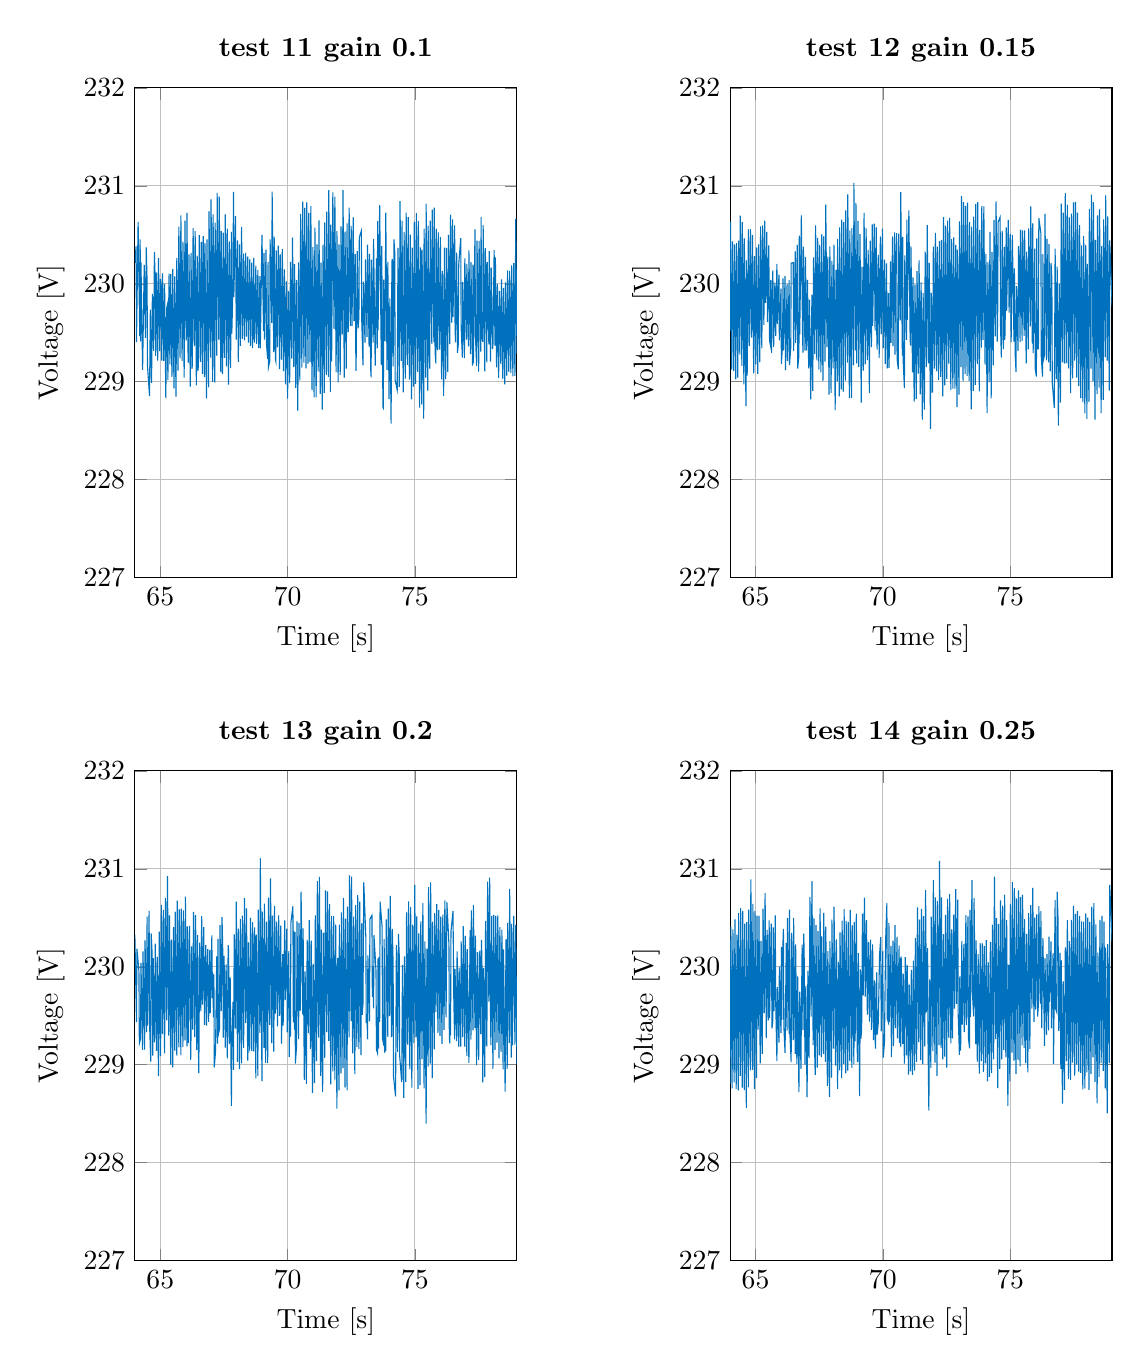
\begin{tikzpicture}

\begin{axis}[%
width=0.4\textwidth,
height=2.449in,
at={(1.024in,4.208in)},
scale only axis,
xmin=64,
xmax=79,
xlabel={Time [s]},
xmajorgrids,
ymin=227,
ymax=232,
ylabel={Voltage [V]},
ymajorgrids,
axis background/.style={fill=white},
title style={font=\bfseries},
title={test 11 gain 0.1}
]
\addplot [color=mycolor1,solid,forget plot]
  table[row sep=crcr]{%
64	230.212749340316\\
64.048	230.382052566566\\
64.064	229.404279023822\\
64.128	230.632602758627\\
64.192	229.468398702534\\
64.208	230.452751786673\\
64.224	229.41328866056\\
64.24	230.218507155381\\
64.304	229.121408875233\\
64.368	230.193425175678\\
64.416	229.448877965094\\
64.448	230.370709114577\\
64.48	230.019319666696\\
64.496	229.161828604992\\
64.576	228.852410440148\\
64.608	229.736533719515\\
64.656	228.987640702386\\
64.688	229.89777059702\\
64.736	229.315984397185\\
64.768	230.324468158748\\
64.8	230.019811448865\\
64.816	229.263612118938\\
64.848	230.114758916535\\
64.896	229.215179258403\\
64.928	230.262117069954\\
64.976	229.313055462848\\
65.008	230.047035933679\\
65.04	229.937689639171\\
65.056	229.215344927019\\
65.088	230.107258703544\\
65.136	229.211921505521\\
65.168	229.995499188594\\
65.216	228.832009419298\\
65.248	229.747652150554\\
65.28	229.786621895682\\
65.296	229.015377288444\\
65.344	230.103154123468\\
65.376	229.178462452276\\
65.408	230.099472930198\\
65.456	229.05009257868\\
65.488	230.149331803042\\
65.536	228.933462523359\\
65.568	230.075531090847\\
65.616	228.849322729114\\
65.648	230.263757902049\\
65.696	229.114644437642\\
65.728	230.583279672685\\
65.776	229.238350046241\\
65.808	230.697667392537\\
65.84	229.712921496981\\
65.856	229.21333026996\\
65.888	230.42923447681\\
65.936	229.0419999733\\
65.968	230.643837707563\\
66.016	229.418587563436\\
66.048	230.724910363322\\
66.08	229.437343007159\\
66.096	229.194439516014\\
66.128	230.300375197077\\
66.176	228.950710595869\\
66.208	230.316505410565\\
66.24	229.132980071657\\
66.256	229.163636267393\\
66.288	230.569400780851\\
66.336	229.3628996326\\
66.368	230.537166978352\\
66.416	228.96256743015\\
66.448	230.287511498806\\
66.48	229.114651642742\\
66.496	229.179109455625\\
66.528	230.497318570785\\
66.576	229.201947244727\\
66.608	230.427332437039\\
66.656	229.079649630878\\
66.672	230.388437426458\\
66.688	230.487005954821\\
66.736	229.047691729505\\
66.752	230.415791193879\\
66.816	228.829464046645\\
66.832	230.454241157364\\
66.896	228.942283267071\\
66.912	230.738957759124\\
66.976	229.24683835808\\
66.992	230.861449377355\\
67.056	228.998000415588\\
67.072	230.708551657044\\
67.136	228.992849211273\\
67.152	230.623778976014\\
67.216	229.267152537648\\
67.232	230.927540313875\\
67.296	229.428964009387\\
67.312	230.891716180825\\
67.376	229.097972288822\\
67.392	230.53674771707\\
67.44	229.077100005258\\
67.472	230.523288056983\\
67.504	229.363314856872\\
67.52	229.243044612312\\
67.552	230.707789029889\\
67.6	229.157528859237\\
67.632	230.564189346777\\
67.68	228.971558520593\\
67.712	230.433996180166\\
67.76	229.138466711436\\
67.792	230.530086661051\\
67.808	229.491133404883\\
67.856	230.002202526477\\
67.872	230.938333880708\\
67.888	229.864716326481\\
67.952	230.6911092455\\
67.984	229.42909310341\\
68.032	230.44236579351\\
68.064	229.203634887825\\
68.08	229.625273572538\\
68.112	230.402467659663\\
68.144	229.365317593097\\
68.192	230.577779408802\\
68.224	229.438313196311\\
68.272	230.308270196976\\
68.304	229.421654809758\\
68.352	230.315020454788\\
68.384	229.461232780738\\
68.432	230.2780655335\\
68.464	229.400284146254\\
68.512	230.248425723527\\
68.544	229.363466475439\\
68.592	230.216931412169\\
68.624	229.342818273658\\
68.672	230.263237621314\\
68.688	229.448494923191\\
68.704	229.399472985486\\
68.752	230.185253723201\\
68.784	229.385811273956\\
68.832	230.138344180035\\
68.864	229.343772953222\\
68.912	230.07793107384\\
68.928	229.340262911971\\
68.992	230.499678378771\\
69.056	229.518785518577\\
69.072	230.31379431343\\
69.088	229.430803367074\\
69.152	230.348779698496\\
69.168	229.389389007984\\
69.216	229.23402628227\\
69.232	230.224281750382\\
69.248	229.148190142165\\
69.296	229.209487364563\\
69.312	230.453406796181\\
69.376	229.601003661617\\
69.392	230.939676483236\\
69.456	229.302613474977\\
69.472	230.481395892125\\
69.52	229.229385111258\\
69.536	229.210545478281\\
69.552	230.341480115333\\
69.6	229.350309669062\\
69.632	230.38880049564\\
69.664	229.962428108913\\
69.68	229.129568855615\\
69.712	230.299366036305\\
69.76	229.226661873108\\
69.792	230.353534755102\\
69.84	229.108476266892\\
69.872	230.147651708112\\
69.888	229.803870349182\\
69.92	228.972317202676\\
69.952	230.024575714353\\
70	228.827930935655\\
70.032	229.923879431945\\
70.08	228.986932716992\\
70.112	230.224768946714\\
70.16	229.236539622819\\
70.192	230.470832295193\\
70.24	229.151558872974\\
70.272	230.201581741809\\
70.32	228.937636349441\\
70.352	230.038218970825\\
70.4	228.705059707861\\
70.432	230.218437455382\\
70.48	229.01411905248\\
70.512	230.714820682924\\
70.56	229.144418945531\\
70.592	230.837754204911\\
70.64	229.196289130583\\
70.672	230.776012370009\\
70.704	229.479446858083\\
70.72	229.137547319248\\
70.752	230.83032736558\\
70.8	229.185677973253\\
70.832	230.724676571598\\
70.88	229.201647927847\\
70.912	230.791644314549\\
70.944	229.343464541726\\
70.96	228.915399999053\\
70.992	230.37482674728\\
71.04	228.840215360789\\
71.072	230.572897328189\\
71.12	228.841071891801\\
71.152	230.402947968105\\
71.2	229.105599300337\\
71.232	230.646873153524\\
71.28	228.875672436824\\
71.312	230.21723745007\\
71.36	228.71516713713\\
71.392	230.400974470409\\
71.44	228.887484895778\\
71.456	230.626171032278\\
71.52	229.071279834368\\
71.536	230.736954612111\\
71.6	229.050176822087\\
71.616	230.954861966236\\
71.68	228.893553997604\\
71.696	230.604471676234\\
71.728	229.207033730061\\
71.776	230.933251765287\\
71.824	229.540741512554\\
71.856	230.888525020352\\
71.904	229.098598570003\\
71.936	230.537266896748\\
71.984	228.993266391598\\
72.016	230.402868930744\\
72.064	229.070102899375\\
72.08	229.598712478919\\
72.096	230.586378730763\\
72.144	229.484035434969\\
72.176	230.957048153871\\
72.224	229.042350185609\\
72.256	230.532217903789\\
72.304	229.133116587476\\
72.336	230.616105848847\\
72.352	229.626795180134\\
72.384	229.505756219912\\
72.416	230.777542935319\\
72.464	229.571353783612\\
72.496	230.591591404701\\
72.528	229.568992810459\\
72.576	230.67845894747\\
72.608	229.619950530819\\
72.656	230.302145511934\\
72.672	229.400325842964\\
72.688	229.110201100843\\
72.736	230.333843262803\\
72.768	229.545917849449\\
72.8	229.660362339739\\
72.816	230.473549305794\\
72.896	230.540161474257\\
72.912	229.6259493958\\
72.96	229.166239298499\\
72.976	230.021526599084\\
73.04	229.399274674862\\
73.056	230.248017898817\\
73.12	229.457507776666\\
73.136	230.39891200691\\
73.2	229.357451032282\\
73.216	230.304273264996\\
73.264	229.120713244394\\
73.28	229.04502465183\\
73.296	230.246102986847\\
73.36	229.399262115911\\
73.376	230.458091098868\\
73.44	229.163505466311\\
73.488	230.258340860279\\
73.52	229.340352280366\\
73.536	230.640822536836\\
73.552	229.523259345065\\
73.616	230.802017524795\\
73.68	229.171888052064\\
73.696	230.384451539763\\
73.744	228.741436948941\\
73.76	228.732490940892\\
73.776	230.042839954544\\
73.824	229.415737136348\\
73.856	230.723063366821\\
73.904	229.120178960103\\
73.92	229.354000822713\\
73.936	230.224110293666\\
73.984	228.823720542887\\
74.016	229.850099145147\\
74.064	228.573222541254\\
74.096	230.222705316333\\
74.112	230.252373503153\\
74.144	229.156618777398\\
74.176	230.453651514564\\
74.208	230.324374549888\\
74.224	229.016851593481\\
74.304	228.915544135857\\
74.336	230.366620853429\\
74.384	228.948369694695\\
74.416	230.844763004116\\
74.464	229.21260534023\\
74.496	230.643028910822\\
74.512	229.674935500377\\
74.544	228.891840543072\\
74.576	230.52926528466\\
74.624	229.031202189745\\
74.656	230.727568497533\\
74.704	229.171363310054\\
74.736	230.680799997484\\
74.752	229.947933925122\\
74.784	229.021582975843\\
74.816	230.503105641653\\
74.864	228.821055011082\\
74.896	230.3698282759\\
74.944	228.949472889332\\
74.976	230.634266609004\\
75.024	228.978836240934\\
75.056	230.720656300714\\
75.104	229.101418062838\\
75.136	230.642654335021\\
75.184	228.734807053024\\
75.216	230.372090925354\\
75.264	228.770323244218\\
75.28	230.348717285917\\
75.344	228.624321098628\\
75.36	230.563135684815\\
75.424	229.042168524784\\
75.44	230.817979084364\\
75.504	228.910622357021\\
75.52	230.594063891146\\
75.552	229.346465826654\\
75.584	229.135131700145\\
75.6	230.644286995033\\
75.664	229.38719258752\\
75.68	230.757110490847\\
75.744	229.405765382365\\
75.76	230.778482279402\\
75.792	229.307777969053\\
75.824	229.185647519041\\
75.84	230.5620117235\\
75.888	229.32183636692\\
75.92	230.523797627327\\
75.936	229.923585764257\\
75.968	229.326835294782\\
76	230.475561417825\\
76.048	229.02400232821\\
76.08	230.132014736203\\
76.128	228.855692393101\\
76.16	230.36948485856\\
76.176	229.654680149937\\
76.208	229.028797873195\\
76.24	230.367506906688\\
76.288	229.100170030824\\
76.32	230.498959961168\\
76.368	229.385020729134\\
76.4	230.706256019752\\
76.448	229.602985580071\\
76.48	230.656656403166\\
76.496	229.662456608139\\
76.56	230.596646734205\\
76.576	229.606073413626\\
76.592	229.400982154896\\
76.64	230.317502987851\\
76.672	229.294469740571\\
76.704	229.38323203506\\
76.72	230.193652897661\\
76.8	230.466032347235\\
76.816	229.556270827401\\
76.864	229.246418601325\\
76.88	230.020651483008\\
76.944	229.24001272119\\
76.96	230.2598154158\\
77.024	229.430181576421\\
77.04	230.202099487249\\
77.104	229.360959917566\\
77.12	230.339913289735\\
77.184	229.280853206208\\
77.2	230.222923220883\\
77.264	229.16495288574\\
77.28	230.196459398217\\
77.296	229.188778386206\\
77.36	230.556301227948\\
77.376	229.473869727338\\
77.424	229.159700242673\\
77.44	230.440077487203\\
77.504	229.102531930812\\
77.52	230.439119212821\\
77.584	229.307860532125\\
77.6	230.683446095326\\
77.616	229.48170650084\\
77.664	229.407489017341\\
77.68	230.598251510723\\
77.744	229.106694796066\\
77.76	230.362900114355\\
77.792	230.097409378589\\
77.824	229.197027209886\\
77.84	230.221463125762\\
77.904	229.382155393596\\
77.92	230.334185139353\\
77.968	229.204301217532\\
78	230.165985674797\\
78.048	229.334513585646\\
78.064	229.368145853649\\
78.112	230.343265194096\\
78.144	229.368870145334\\
78.16	230.268734944404\\
78.208	229.145733348708\\
78.24	229.996981750788\\
78.288	229.040726426139\\
78.32	229.926021730245\\
78.368	229.185237423535\\
78.4	230.045152102233\\
78.448	229.032812776332\\
78.48	229.957595990778\\
78.528	228.972599130904\\
78.56	230.014036703146\\
78.608	229.062373777368\\
78.64	230.136250408662\\
78.688	229.10017544259\\
78.72	230.13128997219\\
78.768	229.090111926433\\
78.784	229.638141371624\\
78.8	230.189025451286\\
78.848	229.055346972886\\
78.88	230.211964205123\\
78.928	229.060379118533\\
78.96	230.661495501455\\
79.008	229.287639260292\\
};
\end{axis}

\begin{axis}[%
width=0.4\textwidth,
height=2.449in,
at={(4in,4.208in)},
scale only axis,
xmin=64,
xmax=79,
xlabel={Time [s]},
xmajorgrids,
ymin=227,
ymax=232,
ylabel={Voltage [V]},
ymajorgrids,
axis background/.style={fill=white},
title style={font=\bfseries},
title={test 12  gain 0.15}
]
\addplot [color=mycolor1,solid,forget plot]
  table[row sep=crcr]{%
64	229.523183449264\\
64.016	230.633985933491\\
64.064	229.124479435671\\
64.096	230.433082440938\\
64.144	229.11208451754\\
64.176	230.402031983288\\
64.224	229.024485078031\\
64.24	229.998146530983\\
64.256	230.415898480736\\
64.304	229.0420926361\\
64.336	230.440160851961\\
64.384	229.276964174602\\
64.4	230.696614719419\\
64.464	229.163180265574\\
64.48	230.629558425434\\
64.544	228.972378365407\\
64.56	230.463192172045\\
64.624	228.752140776427\\
64.64	230.23805287505\\
64.672	229.061543481521\\
64.72	230.556129386367\\
64.752	229.362662469042\\
64.8	230.559082129234\\
64.832	229.493569203895\\
64.848	229.451330850515\\
64.88	230.497547090498\\
64.928	229.086708149813\\
64.96	230.281882384516\\
65.008	229.176508197108\\
65.04	230.371065726741\\
65.072	229.439280974484\\
65.088	229.081272000532\\
65.12	230.402047428448\\
65.168	229.199149592676\\
65.2	230.584991050438\\
65.248	229.341748855\\
65.28	230.595791745566\\
65.328	229.580362697928\\
65.36	230.645837092501\\
65.392	229.804773067181\\
65.424	229.965689832843\\
65.44	230.530830230703\\
65.472	229.608852824486\\
65.52	230.392072963303\\
65.552	229.416658019309\\
65.584	229.374999500788\\
65.6	230.038700757397\\
65.632	229.295049433038\\
65.648	229.840431054505\\
65.68	230.136182411245\\
65.712	229.355456440659\\
65.76	230.012669974121\\
65.792	229.467905762429\\
65.84	230.202243540385\\
65.856	229.590392024565\\
65.92	230.093051906042\\
65.936	229.421310758924\\
66	229.949663260448\\
66.016	229.180783023429\\
66.064	229.385250066594\\
66.08	230.054145570439\\
66.096	229.319226155882\\
66.16	230.078661772741\\
66.176	229.119204980892\\
66.24	229.995947661638\\
66.256	229.209636651045\\
66.32	230.03708426283\\
66.336	229.170186446056\\
66.384	229.348013468635\\
66.4	230.210084988214\\
66.48	230.216856391955\\
66.496	229.31585531915\\
66.56	230.330565049705\\
66.576	229.398002094266\\
66.64	230.396736393021\\
66.656	229.135380749\\
66.704	229.26598838038\\
66.72	230.492877572148\\
66.736	229.483879510891\\
66.8	230.697330855885\\
66.848	229.461770709935\\
66.864	229.297924563778\\
66.88	230.37991550758\\
66.944	229.317543075439\\
66.96	230.273715782033\\
67.008	229.319450313007\\
67.04	230.040313885323\\
67.088	229.136946121938\\
67.12	229.838981206711\\
67.168	228.820785556188\\
67.216	229.888755290175\\
67.248	228.905703812311\\
67.28	230.270050231433\\
67.328	229.285408882273\\
67.36	230.595761368647\\
67.408	229.217478233119\\
67.44	230.467699811909\\
67.456	230.208152245718\\
67.488	229.124602151488\\
67.52	230.396261539268\\
67.568	229.096919455919\\
67.6	230.503928288637\\
67.648	229.007443293327\\
67.68	230.483840072479\\
67.728	229.205723849945\\
67.76	230.808379070564\\
67.808	229.354297019207\\
67.84	230.278170742545\\
67.888	228.869779041391\\
67.92	230.381105127454\\
67.968	228.887070936122\\
68	230.232945049973\\
68.048	229.137793161006\\
68.08	230.400099233869\\
68.128	228.709637614437\\
68.16	230.140853540892\\
68.208	229.003808925674\\
68.224	230.459110180885\\
68.272	229.337277918074\\
68.288	228.850687302809\\
68.304	230.576183908814\\
68.368	228.922995168945\\
68.384	230.655819414049\\
68.448	228.898259584554\\
68.464	230.629071886523\\
68.512	229.504593836561\\
68.528	229.012458831006\\
68.544	230.749858296577\\
68.608	229.195470145296\\
68.624	230.911524872929\\
68.64	230.309842343187\\
68.688	228.831836322511\\
68.704	230.545701626002\\
68.768	228.836332324674\\
68.784	230.567352521629\\
68.848	229.168475746263\\
68.864	231.030939865804\\
68.88	230.492068206029\\
68.928	229.320431824736\\
68.944	230.826751771187\\
68.976	229.186800446313\\
69.024	230.642128459418\\
69.056	229.150788747505\\
69.104	230.507564361371\\
69.152	228.78806794665\\
69.184	230.172000294513\\
69.232	229.113342520656\\
69.264	230.723226654617\\
69.312	229.177590746727\\
69.344	230.566918951171\\
69.392	229.221832675084\\
69.424	230.34654497648\\
69.472	228.884591527328\\
69.504	230.440704217182\\
69.552	229.3547591749\\
69.584	230.605982181966\\
69.6	229.57155360526\\
69.664	230.615096020655\\
69.696	229.5217574016\\
69.744	230.576198883345\\
69.76	229.519385159498\\
69.776	229.327742626629\\
69.824	230.296298263625\\
69.856	229.245002926797\\
69.904	230.484160985445\\
69.936	229.484260863719\\
69.984	230.562598373015\\
70.016	229.344514444042\\
70.064	230.245445632489\\
70.096	229.181237871197\\
70.144	230.208369698867\\
70.176	229.137487708366\\
70.224	229.904241180026\\
70.24	229.140745971563\\
70.272	229.483130714753\\
70.304	230.229026766627\\
70.32	229.396233150534\\
70.384	230.48401989237\\
70.4	229.364491292323\\
70.464	230.524544535575\\
70.48	229.275992064651\\
70.496	230.143920562607\\
70.544	230.516324910783\\
70.56	229.232916857509\\
70.608	229.127683116867\\
70.624	230.512607045753\\
70.688	229.627742921952\\
70.704	230.935192707477\\
70.768	229.265739632958\\
70.784	230.478284946295\\
70.8	229.207911291781\\
70.848	228.934724884273\\
70.864	230.29019559836\\
70.928	229.427054115605\\
70.944	230.655479185348\\
70.96	229.630708468257\\
71.024	230.749406651915\\
71.072	229.438744726977\\
71.088	229.368555440503\\
71.104	230.381195501662\\
71.168	229.094800994358\\
71.184	230.065447764736\\
71.232	228.797832217694\\
71.264	229.991334367614\\
71.312	228.824668783272\\
71.344	230.128390389633\\
71.392	229.083744284838\\
71.424	230.238837315213\\
71.472	228.871833390595\\
71.488	229.464810006634\\
71.504	230.013481594448\\
71.552	228.614146303546\\
71.584	229.905512487966\\
71.632	228.715132468067\\
71.664	230.327466950394\\
71.712	229.148338765821\\
71.744	230.598511549314\\
71.792	229.187579686817\\
71.824	230.213699147782\\
71.872	228.520033728644\\
71.904	229.906273831982\\
71.952	228.889301839397\\
71.984	230.37834568883\\
72.032	229.133426987284\\
72.064	230.520767861397\\
72.08	230.271306607924\\
72.112	229.108374431669\\
72.144	230.378986444165\\
72.192	229.015789693511\\
72.224	230.434573281069\\
72.272	229.049807916189\\
72.304	230.44943723236\\
72.32	229.725994659271\\
72.352	228.849840928807\\
72.384	230.679714667206\\
72.432	228.963384242342\\
72.464	230.594211602594\\
72.512	229.028745638923\\
72.544	230.645652184774\\
72.592	229.182901201473\\
72.624	230.673324024486\\
72.672	228.913568502748\\
72.704	230.455208561934\\
72.752	228.928935342052\\
72.784	230.474171267335\\
72.832	228.931012468875\\
72.864	230.397310783576\\
72.912	228.739921369481\\
72.928	230.34909298759\\
72.992	228.86857145117\\
73.008	230.637148698849\\
73.072	229.149135814195\\
73.088	230.895329898238\\
73.136	229.492683150933\\
73.152	229.005902095008\\
73.168	230.833148003415\\
73.232	229.07860117059\\
73.248	230.796265311823\\
73.312	229.061085596491\\
73.328	230.827988692999\\
73.36	229.568718933636\\
73.392	229.006038405052\\
73.408	230.629109458265\\
73.472	228.719235066768\\
73.488	230.58321521679\\
73.504	230.317727597836\\
73.552	228.905667259006\\
73.568	230.685761858405\\
73.632	228.969238173277\\
73.648	230.81437945657\\
73.712	229.179527150766\\
73.728	230.832719115091\\
73.744	230.196221128419\\
73.792	228.902896646071\\
73.808	230.550660003453\\
73.872	229.349072260908\\
73.888	230.794948708017\\
73.936	229.427462181468\\
73.968	230.790978230903\\
74.016	229.174694489508\\
74.048	230.301826097858\\
74.096	228.679994709275\\
74.128	230.22174142145\\
74.176	228.994931908525\\
74.208	230.529515857714\\
74.256	228.829295289017\\
74.288	230.326879398791\\
74.336	229.167889296063\\
74.368	230.651365257979\\
74.416	229.462943617829\\
74.448	230.84213113261\\
74.496	229.409080236664\\
74.512	229.713523924511\\
74.528	230.628025478246\\
74.608	230.680494821029\\
74.624	229.56137141341\\
74.656	229.247347610504\\
74.688	230.540680985065\\
74.736	229.332654073711\\
74.768	230.377064527376\\
74.784	229.428084404889\\
74.8	229.478976690674\\
74.848	230.575068979821\\
74.864	229.724772683691\\
74.928	230.651387923606\\
74.96	229.70582651511\\
75.008	230.509085860294\\
75.04	229.404462287035\\
75.088	230.497103927966\\
75.152	229.409924413014\\
75.168	230.157512935891\\
75.2	229.276594892269\\
75.232	229.099266810719\\
75.248	229.975973831624\\
75.312	229.315380310963\\
75.328	230.38315908782\\
75.36	230.233843722724\\
75.392	229.403527894212\\
75.408	230.553695973405\\
75.472	229.417119360599\\
75.488	230.546411621739\\
75.552	229.468836617912\\
75.568	230.545342237479\\
75.632	229.188258790895\\
75.648	230.328559457196\\
75.712	229.33124182363\\
75.728	230.565728236831\\
75.792	229.564464595267\\
75.808	230.790771892548\\
75.872	229.389490162285\\
75.888	230.617419531988\\
75.904	229.293425933548\\
75.968	230.359606255792\\
75.984	229.135198679678\\
76.032	229.053056721185\\
76.048	230.462858600877\\
76.064	229.334452349192\\
76.112	229.337207774047\\
76.128	230.672983183982\\
76.208	230.516748167164\\
76.224	229.256789623835\\
76.272	229.052417394667\\
76.288	230.302267512725\\
76.304	229.218088403885\\
76.352	229.276295106033\\
76.368	230.712500087311\\
76.432	229.217848325412\\
76.448	230.459215279803\\
76.512	229.197617436766\\
76.528	230.406057497659\\
76.576	229.106267144451\\
76.608	230.211301517629\\
76.64	230.051720440459\\
76.656	228.990108642532\\
76.736	228.734087936186\\
76.768	230.359954475508\\
76.816	229.027276582437\\
76.848	230.174857260425\\
76.896	228.550948200957\\
76.928	230.00010246687\\
76.944	229.753510409574\\
76.976	228.787602103521\\
77.008	230.818493565974\\
77.056	229.197926152858\\
77.088	230.725487637147\\
77.136	229.18632570533\\
77.168	230.925562074171\\
77.184	230.187745213037\\
77.216	229.190629251533\\
77.248	230.808049847009\\
77.296	229.137542160226\\
77.328	230.678803385397\\
77.376	228.884646800363\\
77.408	230.716795510936\\
77.456	229.035699192126\\
77.488	230.831278380312\\
77.536	229.215469812703\\
77.568	230.837102943062\\
77.616	229.040999931402\\
77.648	230.725429779499\\
77.696	228.957410371289\\
77.728	230.598020258372\\
77.776	228.834010696844\\
77.808	230.390913388557\\
77.856	228.791216774368\\
77.888	230.487520233867\\
77.936	228.676285337125\\
77.968	230.397218314759\\
78	229.339378154831\\
78.016	228.621450906003\\
78.032	230.204470869515\\
78.096	228.794811879596\\
78.112	230.764368131689\\
78.176	229.133856827974\\
78.192	230.909447689884\\
78.24	229.866834847741\\
78.256	229.004812236469\\
78.272	230.834630860609\\
78.336	228.613353207951\\
78.352	230.444509217492\\
78.368	230.216288295255\\
78.416	228.874821582285\\
78.432	230.699138834522\\
78.496	228.941174571599\\
78.512	230.760381585835\\
78.576	228.67984457639\\
78.592	230.384296604201\\
78.608	230.033567578646\\
78.656	228.813775705048\\
78.672	230.658116641147\\
78.736	229.251468638458\\
78.752	230.90282848808\\
78.816	229.216910353185\\
78.832	230.687050889631\\
78.896	228.908213371978\\
78.912	230.442688200989\\
79.008	229.769782418665\\
};
\end{axis}

\begin{axis}[%
width=0.4\textwidth,
height=2.449in,
at={(1.024in,0.793in)},
scale only axis,
xmin=64,
xmax=79,
xlabel={Time [s]},
xmajorgrids,
ymin=227,
ymax=232,
ylabel={Voltage [V]},
ymajorgrids,
axis background/.style={fill=white},
title style={font=\bfseries},
title={test 13  gain 0.2}
]
\addplot [color=mycolor1,solid,forget plot]
  table[row sep=crcr]{%
64	230.328289053422\\
64.064	229.435353090832\\
64.08	230.186273286632\\
64.16	229.956780599981\\
64.176	229.21827020465\\
64.224	229.263274719667\\
64.24	230.040898939298\\
64.304	229.152475556633\\
64.32	230.157627333503\\
64.384	229.154753362428\\
64.4	230.268495765389\\
64.464	229.332865504586\\
64.48	230.512235711732\\
64.496	229.399172451688\\
64.56	230.571489346586\\
64.576	229.428979406903\\
64.624	229.032325445592\\
64.64	230.34081641224\\
64.672	230.16983745385\\
64.704	229.093218719804\\
64.72	230.088993174481\\
64.768	229.228014273476\\
64.784	229.528164603512\\
64.8	230.237119161192\\
64.848	229.141074252535\\
64.88	230.100470534755\\
64.928	228.883757768969\\
64.96	230.357677722107\\
65.008	229.087587844508\\
65.024	229.527094780335\\
65.04	230.632411383083\\
65.088	229.312698998375\\
65.12	230.581176482132\\
65.168	229.11553313324\\
65.2	230.704002157765\\
65.248	229.453800601259\\
65.28	230.926304409999\\
65.328	229.297342624866\\
65.36	230.52444870626\\
65.408	229.000902191375\\
65.424	229.63052364354\\
65.44	230.277515205491\\
65.488	228.973443210825\\
65.52	230.404256082582\\
65.568	229.144961260772\\
65.584	230.564305650169\\
65.648	229.093526319007\\
65.664	230.676168409399\\
65.728	229.178179207985\\
65.744	230.586521155202\\
65.808	229.097198459155\\
65.824	230.594754571711\\
65.888	229.180156835417\\
65.904	230.575768276955\\
65.968	229.249821812137\\
65.984	230.715496286007\\
66.048	229.186995903727\\
66.064	230.413473431844\\
66.096	229.222643913656\\
66.144	230.416862512675\\
66.192	229.049151623285\\
66.208	229.335930406963\\
66.224	230.207204285506\\
66.272	229.35962053781\\
66.304	230.560907340122\\
66.352	229.282386673558\\
66.384	230.528318237975\\
66.432	229.151130612652\\
66.464	230.325189714972\\
66.48	229.399834534277\\
66.512	228.911551333846\\
66.544	230.24560276539\\
66.592	229.547763719953\\
66.624	230.516327985312\\
66.656	229.614988707337\\
66.704	230.404449954464\\
66.736	229.405977878023\\
66.784	230.220668725248\\
66.816	229.399039526705\\
66.832	229.95407807166\\
66.864	230.180717800781\\
66.896	229.437595647302\\
66.944	230.171639552675\\
66.96	229.527780034221\\
67.024	230.319936529632\\
67.04	229.678925782154\\
67.056	229.948056220053\\
67.088	229.482523390778\\
67.104	229.921901840901\\
67.12	228.973782762035\\
67.168	229.136431593818\\
67.216	230.106235964821\\
67.248	229.216253215495\\
67.264	230.283844876858\\
67.28	229.309643706218\\
67.328	229.36934793366\\
67.344	230.424073787258\\
67.392	229.546782231718\\
67.424	230.505831678998\\
67.456	230.120965262872\\
67.472	229.277952101131\\
67.504	230.111290693709\\
67.552	229.173896451433\\
67.584	230.02381261847\\
67.632	229.064518589264\\
67.664	230.221157979777\\
67.68	230.17338297074\\
67.712	229.209906161119\\
67.744	229.892172167625\\
67.792	228.580807645309\\
67.808	229.237605650695\\
67.856	229.641077105135\\
67.872	228.947426988003\\
67.904	230.329933825161\\
67.952	229.367605230682\\
67.984	230.664829004147\\
68.032	229.028118764195\\
68.064	230.389713958831\\
68.096	229.545670965326\\
68.112	228.954675373537\\
68.144	230.485580081924\\
68.192	229.014683104829\\
68.224	230.522632381892\\
68.272	229.171212246431\\
68.304	230.700263226937\\
68.352	229.428310716552\\
68.384	230.595832920178\\
68.432	229.042576762916\\
68.464	230.250069006707\\
68.496	229.155718590585\\
68.512	229.169875702882\\
68.544	230.499886728863\\
68.592	229.140456141679\\
68.624	230.455724570715\\
68.672	229.13508973885\\
68.688	230.19044626237\\
68.704	230.401936281384\\
68.752	228.861506322029\\
68.768	230.328259250463\\
68.832	228.886311755597\\
68.848	230.582679376974\\
68.912	229.324838882609\\
68.928	231.107975593185\\
68.992	228.833595911317\\
69.008	230.563757249809\\
69.072	229.173457953442\\
69.088	230.645331031476\\
69.136	229.020241364391\\
69.168	230.460778445701\\
69.216	229.015986595437\\
69.232	229.73857947825\\
69.248	230.705990298672\\
69.296	229.407340124388\\
69.328	230.902093252397\\
69.376	229.22184793092\\
69.408	230.523254879085\\
69.456	229.133487748128\\
69.488	230.622533561477\\
69.52	229.522078817025\\
69.568	230.46125000553\\
69.6	229.392841003923\\
69.648	230.524709673108\\
69.68	229.499511851916\\
69.728	230.419703274117\\
69.76	229.214529106049\\
69.808	230.128603518009\\
69.824	229.398740454392\\
69.888	230.474082575583\\
69.904	229.659172505225\\
69.968	230.388593961726\\
69.984	229.330806781769\\
70.048	230.160647336252\\
70.064	229.080115984009\\
70.08	229.726230548889\\
70.112	229.287254412248\\
70.128	230.450492523042\\
70.208	230.618556070578\\
70.224	229.432651358816\\
70.24	230.367813283592\\
70.272	229.35921188293\\
70.288	230.353074591048\\
70.304	229.010648656017\\
70.352	229.190818604502\\
70.368	230.463654899599\\
70.432	229.261324513785\\
70.448	230.445895453973\\
70.496	229.551749836982\\
70.528	230.768078617746\\
70.592	229.515367521107\\
70.608	230.391939197406\\
70.656	228.845847157326\\
70.688	229.952707101521\\
70.736	228.804841326799\\
70.768	230.275834537765\\
70.816	229.323430992701\\
70.848	230.476923926596\\
70.896	229.161695581833\\
70.928	230.267301868147\\
70.976	228.713191870422\\
71.008	230.030205140344\\
71.056	228.812736002379\\
71.072	229.519787672769\\
71.088	230.523962847459\\
71.136	229.03781025963\\
71.168	230.874588389142\\
71.216	229.277848804211\\
71.248	230.918032686609\\
71.296	228.885504484089\\
71.328	230.380025513849\\
71.36	228.963430439343\\
71.376	228.719493771491\\
71.408	230.345125473575\\
71.456	229.069908824626\\
71.488	230.780022747062\\
71.536	229.333090565799\\
71.568	230.769896935692\\
71.616	229.244865165864\\
71.648	230.639142512055\\
71.696	228.798651313429\\
71.712	229.617843183438\\
71.728	230.517428602893\\
71.776	228.933236432184\\
71.808	230.517269544122\\
71.856	228.848242466089\\
71.888	230.430588232174\\
71.936	228.552572826044\\
71.952	229.892054924517\\
71.968	230.090185735122\\
72.016	228.73731013041\\
72.032	230.429293593481\\
72.096	228.911452636689\\
72.112	230.556057620557\\
72.176	228.966575981567\\
72.192	230.703340854071\\
72.256	228.767582427644\\
72.272	230.491000549957\\
72.336	228.738737832128\\
72.352	230.613849050261\\
72.416	229.28003073623\\
72.432	230.932720092779\\
72.496	229.445137420847\\
72.512	230.921627777735\\
72.544	229.323576286692\\
72.56	229.115139401377\\
72.592	230.511779577294\\
72.64	228.905230055282\\
72.672	230.630635630025\\
72.72	229.182820668837\\
72.752	230.732489209556\\
72.768	229.760772783451\\
72.8	229.159459066669\\
72.832	230.664283912019\\
72.88	229.097230965278\\
72.912	230.443170512286\\
72.928	229.508490555947\\
72.96	229.618801147071\\
72.992	230.860525988687\\
73.072	230.299260084078\\
73.088	229.424581451048\\
73.12	229.519388886609\\
73.136	229.259024636437\\
73.152	230.116712340092\\
73.216	229.443545123283\\
73.232	230.486988840413\\
73.312	230.526622616358\\
73.328	229.6922644257\\
73.36	229.818181350919\\
73.376	229.575399328724\\
73.392	230.321778061577\\
73.472	229.956048424491\\
73.488	229.15483062918\\
73.536	229.115090288858\\
73.552	230.082796885933\\
73.568	229.163717134919\\
73.584	230.098767075738\\
73.616	229.436546740951\\
73.632	230.666255214147\\
73.712	230.404567325584\\
73.728	229.268395622725\\
73.776	229.19658464739\\
73.792	230.281170691808\\
73.808	229.132148292315\\
73.856	229.148103711365\\
73.872	230.485075217857\\
73.936	229.281064330727\\
73.952	230.592472544769\\
74	229.49594155412\\
74.032	230.724683223294\\
74.08	229.290170101548\\
74.096	229.294018335604\\
74.112	230.387298615355\\
74.144	230.025540460471\\
74.16	228.878603708662\\
74.24	228.676353029537\\
74.272	230.221423150533\\
74.32	229.130061102648\\
74.336	229.679760821364\\
74.352	230.336364039084\\
74.384	230.121914558606\\
74.4	229.094422393274\\
74.48	228.821735476916\\
74.512	230.018245648424\\
74.56	228.662169330863\\
74.592	230.107464688749\\
74.64	228.821661886555\\
74.672	230.554310232532\\
74.72	229.204637281638\\
74.752	230.66849984198\\
74.8	228.953188984737\\
74.832	230.610924834977\\
74.88	228.765889567063\\
74.912	230.430556992844\\
74.96	229.221474092008\\
74.976	229.787708860346\\
74.992	230.837343864501\\
75.04	229.279800197424\\
75.072	230.513830220183\\
75.104	229.220514824292\\
75.12	228.75439634358\\
75.152	230.340171283041\\
75.2	228.792988465477\\
75.216	229.974353434793\\
75.232	230.462314552651\\
75.28	229.057764417392\\
75.312	230.650770543278\\
75.36	228.75930210024\\
75.392	230.258245386988\\
75.44	228.398995853355\\
75.472	230.186441489389\\
75.52	228.981512396717\\
75.536	230.812610697447\\
75.6	229.012500175928\\
75.616	230.862847064207\\
75.68	228.863552593464\\
75.696	230.461812715682\\
75.76	229.155976281279\\
75.776	230.547373160362\\
75.824	229.536634605882\\
75.856	230.63927185615\\
75.904	229.326508404648\\
75.936	230.577673057511\\
75.984	229.29597443853\\
76.016	230.512704309149\\
76.064	229.212460726062\\
76.096	230.531414378665\\
76.144	229.356000133545\\
76.176	230.677239581332\\
76.224	229.48468592468\\
76.256	230.659737194552\\
76.336	230.230232728929\\
76.352	229.276349684655\\
76.368	229.218631726922\\
76.384	229.620157034153\\
76.4	229.299949295094\\
76.416	230.361104522399\\
76.496	230.569270277542\\
76.528	229.653027721851\\
76.56	229.25826061728\\
76.576	229.977451474813\\
76.64	229.242122251378\\
76.656	230.158195689222\\
76.72	229.18388671581\\
76.736	229.991197178616\\
76.8	229.185612640088\\
76.816	230.259543088275\\
76.88	229.281769375106\\
76.896	230.414296927961\\
76.96	229.181784976087\\
76.976	230.316301342393\\
77.04	229.091157545252\\
77.056	230.180870931996\\
77.12	229.018515531604\\
77.168	230.374054128399\\
77.2	229.256783991638\\
77.216	230.576842576206\\
77.28	229.352154507575\\
77.296	230.631517600725\\
77.36	229.376111734783\\
77.376	230.317151252194\\
77.424	228.995796627047\\
77.456	230.15069520005\\
77.504	229.049887454927\\
77.536	230.122126312725\\
77.552	230.164785206252\\
77.584	229.312731629233\\
77.616	230.275629662245\\
77.648	229.77574288684\\
77.664	228.820569902509\\
77.696	229.988577440098\\
77.744	228.873167037516\\
77.776	230.467945517554\\
77.824	229.184412978843\\
77.856	230.870549584719\\
77.904	229.64387694929\\
77.936	230.910493498447\\
77.952	229.916470612175\\
77.984	229.200307902738\\
78.016	230.519226521855\\
78.064	228.958372159578\\
78.096	230.529740130514\\
78.144	229.150967974066\\
78.176	230.518831311348\\
78.224	229.225318409862\\
78.24	230.056796402397\\
78.256	230.523668673168\\
78.304	229.065830160497\\
78.336	230.406039444576\\
78.384	229.130260770816\\
78.416	230.380168304498\\
78.464	228.953036170692\\
78.48	230.178316187202\\
78.544	228.726277499533\\
78.576	230.279452100356\\
78.624	228.957199584971\\
78.64	230.447232973115\\
78.704	229.223138488509\\
78.72	230.795172936267\\
78.784	229.072244720069\\
78.8	230.437320895116\\
78.832	229.197718878181\\
78.88	230.519557898213\\
78.928	229.205645088068\\
78.96	230.426842679965\\
79.008	229.000625766044\\
};
\end{axis}

\begin{axis}[%
width=0.4\textwidth,
height=2.449in,
at={(4in,0.793in)},
scale only axis,
xmin=64,
xmax=79,
xlabel={Time [s]},
xmajorgrids,
ymin=227,
ymax=232,
ylabel={Voltage [V]},
ymajorgrids,
axis background/.style={fill=white},
title style={font=\bfseries},
title={test 14  gain 0.25}
]
\addplot [color=mycolor1,solid,forget plot]
  table[row sep=crcr]{%
64	228.808332987014\\
64.032	230.410753080596\\
64.08	228.758764827421\\
64.112	230.382746946501\\
64.16	228.820524449118\\
64.192	230.48438595689\\
64.24	228.752235296246\\
64.272	230.327994810439\\
64.32	228.739357901061\\
64.336	230.547802165027\\
64.4	228.886297921629\\
64.416	230.599894793416\\
64.48	228.767733243833\\
64.496	230.570139915882\\
64.56	228.741353907687\\
64.576	230.441291434274\\
64.64	228.557100386217\\
64.656	230.454703647698\\
64.72	228.768157289125\\
64.736	230.582536761039\\
64.8	228.94308208746\\
64.816	230.893286838111\\
64.88	228.948614370436\\
64.896	230.641613291269\\
64.96	228.750718270499\\
64.976	230.571473586131\\
65.04	228.862974099333\\
65.056	230.521228405695\\
65.104	229.358273667595\\
65.136	230.518987833977\\
65.184	229.01451878911\\
65.2	229.327490336912\\
65.216	230.264205616063\\
65.264	229.11220385893\\
65.296	230.594374545231\\
65.344	229.527495838994\\
65.376	230.750938457912\\
65.424	229.27093234655\\
65.456	230.376148288562\\
65.504	229.452330836762\\
65.536	230.473727578755\\
65.552	229.476755169255\\
65.616	230.439703909024\\
65.648	229.370664928661\\
65.68	229.454021507633\\
65.696	230.40195071089\\
65.728	229.547406762818\\
65.776	230.525943275202\\
65.792	229.647055732899\\
65.84	229.040797231324\\
65.856	229.792702546634\\
65.92	229.225293416248\\
65.936	230.001734346542\\
66	229.322196551979\\
66.016	230.202111086665\\
66.032	229.457010571963\\
66.048	230.017341205343\\
66.096	230.386774841253\\
66.112	229.395886485033\\
66.16	229.12187072883\\
66.208	230.244768654032\\
66.24	229.347802093271\\
66.256	230.497909870849\\
66.32	229.316051773525\\
66.336	230.583305913005\\
66.352	229.305403306902\\
66.4	229.028066851377\\
66.416	230.346677944668\\
66.48	229.250878636825\\
66.496	230.498760393159\\
66.56	229.111994958361\\
66.576	230.229598907308\\
66.624	229.009893255498\\
66.656	229.902312894564\\
66.704	228.720472540513\\
66.736	229.746100947818\\
66.784	228.9576434636\\
66.8	229.502283813655\\
66.832	230.226222497829\\
66.864	229.356629004225\\
66.896	230.33781128463\\
66.912	230.091615332995\\
66.944	229.001285237685\\
66.976	229.804830215011\\
67.024	228.670808467104\\
67.04	229.096472342598\\
67.056	229.959088494819\\
67.104	229.067778978356\\
67.136	230.710754254629\\
67.184	229.490474097835\\
67.216	230.875350666345\\
67.264	229.200676094294\\
67.296	230.495291167212\\
67.328	229.079770536699\\
67.344	228.897291801666\\
67.376	230.425297300127\\
67.424	228.969482203838\\
67.456	230.364916683749\\
67.504	229.095381922161\\
67.536	230.597257164044\\
67.584	229.078140644964\\
67.6	230.310146772907\\
67.664	229.110913380901\\
67.68	230.550558413864\\
67.744	229.030390697026\\
67.76	230.410503053532\\
67.824	228.7837001551\\
67.84	230.159631493526\\
67.904	228.671434708519\\
67.92	230.261073309741\\
67.984	228.867352538461\\
68	230.481348241782\\
68.064	229.164519087418\\
68.08	230.614110208737\\
68.096	230.379003862968\\
68.144	228.991384849035\\
68.176	230.28023731949\\
68.224	228.754981486048\\
68.256	230.048944394934\\
68.304	228.943359879386\\
68.32	230.351012510785\\
68.384	228.864610339874\\
68.4	230.471887131497\\
68.464	229.010038104983\\
68.48	230.587710574332\\
68.544	228.911942742949\\
68.56	230.4676647458\\
68.624	228.939522515246\\
68.64	230.458054389818\\
68.672	229.335007100034\\
68.704	229.037676769506\\
68.72	230.581296288995\\
68.784	228.967482638469\\
68.8	230.422158972722\\
68.864	229.002891547572\\
68.88	230.459519931424\\
68.912	229.237711039744\\
68.96	230.543603816326\\
68.992	229.177866187194\\
69.008	229.026702540134\\
69.04	230.139917642436\\
69.088	228.679757176648\\
69.104	229.319533818029\\
69.12	229.972433931785\\
69.136	229.264713791249\\
69.168	229.343972525337\\
69.2	230.541488130243\\
69.232	229.708919523864\\
69.28	230.706256697075\\
69.312	229.694245543754\\
69.36	230.475506698308\\
69.392	229.511638653504\\
69.44	230.251994538298\\
69.472	229.439892584272\\
69.52	230.276821985041\\
69.552	229.356945671148\\
69.6	230.228949613962\\
69.632	229.252363715056\\
69.68	229.862228150589\\
69.696	229.266659795923\\
69.712	229.164194983114\\
69.76	229.942090009778\\
69.776	229.307443494327\\
69.824	229.430865280355\\
69.872	230.125166791213\\
69.92	230.302281882204\\
69.936	229.341631055623\\
70	230.161995766983\\
70.016	229.072030525114\\
70.064	229.223811872511\\
70.112	230.280904530512\\
70.16	230.650778463552\\
70.176	229.469437184576\\
70.224	229.428669027088\\
70.24	230.448642703926\\
70.256	229.438366426027\\
70.32	230.21088845171\\
70.336	229.077250586953\\
70.4	230.267132340955\\
70.416	229.190481964533\\
70.48	230.424843135177\\
70.496	229.373375775543\\
70.56	230.306315575524\\
70.576	229.268776383073\\
70.64	230.214919613632\\
70.656	229.223747779236\\
70.672	230.090503756032\\
70.704	229.184342605276\\
70.72	230.107194687074\\
70.784	229.213770517086\\
70.8	229.929850803647\\
70.848	229.012399540945\\
70.88	230.098256795343\\
70.912	229.85164593219\\
70.928	229.095613608368\\
70.96	230.013345739646\\
71.008	228.899393158278\\
71.04	229.817686724998\\
71.088	228.932858970936\\
71.12	229.967387934948\\
71.168	228.896130222696\\
71.2	230.063737434376\\
71.248	228.939102328536\\
71.28	230.293682304001\\
71.328	229.029595952142\\
71.36	230.606509096703\\
71.408	229.23181864997\\
71.44	230.482701889723\\
71.488	229.047259291304\\
71.52	230.591308957639\\
71.568	229.005763823754\\
71.6	230.518005191788\\
71.648	229.186384192153\\
71.68	230.782261221854\\
71.712	229.534491864754\\
71.76	230.189653601316\\
71.776	229.224830345038\\
71.808	228.531631522027\\
71.84	229.870899149364\\
71.888	228.966852752859\\
71.904	230.512835019412\\
71.952	229.639065833764\\
71.968	229.139945242393\\
71.984	230.884597461263\\
72.048	229.022488475565\\
72.064	230.708560570833\\
72.08	230.256121121696\\
72.128	228.885603378114\\
72.144	230.672494473291\\
72.208	229.201053619762\\
72.224	231.081837729691\\
72.288	229.173446587344\\
72.304	230.708893383581\\
72.32	229.887334853045\\
72.352	229.054678181021\\
72.384	230.333189589987\\
72.432	229.082437067332\\
72.464	230.529474716875\\
72.512	228.971933224964\\
72.544	230.693203393445\\
72.592	229.272633403515\\
72.624	230.741454600639\\
72.672	229.217228295642\\
72.704	230.381923361291\\
72.736	229.269993605794\\
72.784	230.532471947386\\
72.816	229.571719361602\\
72.864	230.792901185146\\
72.896	229.621494563425\\
72.944	230.686436272243\\
72.96	229.518190041076\\
73.008	229.100722545443\\
73.024	229.902200715834\\
73.056	229.144992382304\\
73.104	230.262411452101\\
73.12	229.408995746526\\
73.184	230.233287335724\\
73.2	229.333647593117\\
73.264	230.52621356362\\
73.28	229.408000853033\\
73.344	230.513518115339\\
73.36	229.278301172863\\
73.408	229.168433693185\\
73.424	230.580593605577\\
73.44	229.488381986336\\
73.504	230.885346364421\\
73.52	229.729288174893\\
73.568	229.494182245958\\
73.584	230.700436568463\\
73.648	229.211534119592\\
73.664	230.270004555413\\
73.712	229.032417218206\\
73.744	230.128530968758\\
73.792	228.909581057288\\
73.824	230.240406759793\\
73.872	229.036053430744\\
73.904	230.239661845875\\
73.92	230.044108037114\\
73.952	228.928536429789\\
73.984	230.211782703664\\
74.032	229.01300903222\\
74.064	230.272608810392\\
74.112	228.829682284167\\
74.144	230.044093854382\\
74.192	228.876570508937\\
74.224	230.254279936443\\
74.272	228.913590967084\\
74.304	230.431441568378\\
74.352	229.054128097326\\
74.384	230.920995356832\\
74.432	229.26113121756\\
74.464	230.49778205926\\
74.512	228.760442740989\\
74.544	230.436316041994\\
74.592	228.958111689144\\
74.624	230.676973918427\\
74.672	229.054208967405\\
74.704	230.623102690213\\
74.752	229.151265348024\\
74.784	230.735725441797\\
74.832	229.075028115449\\
74.864	230.477296912934\\
74.912	228.579124989322\\
74.944	230.018363005266\\
74.976	229.098872172072\\
74.992	228.831538156757\\
75.008	230.642489254902\\
75.072	229.123365308329\\
75.088	230.865474232123\\
75.152	229.042848430225\\
75.168	230.802067372407\\
75.2	229.443137402685\\
75.232	228.907432580751\\
75.248	230.699577395997\\
75.312	229.049364965529\\
75.328	230.779358592181\\
75.344	230.380015204029\\
75.392	228.983192450184\\
75.408	230.710929428499\\
75.472	229.197575707609\\
75.488	230.732837386801\\
75.552	229.173010712153\\
75.568	230.485274843795\\
75.616	229.016990635573\\
75.648	230.333509495\\
75.696	228.922835565929\\
75.728	230.548017882389\\
75.776	229.161451731108\\
75.808	230.63061696164\\
75.856	229.57397264579\\
75.888	230.806646459031\\
75.936	229.438335502149\\
75.968	230.501216197212\\
76	229.563287985504\\
76.048	230.533812339296\\
76.08	229.491994537236\\
76.112	229.617285321018\\
76.128	230.619520413807\\
76.192	229.624977102573\\
76.208	230.569428438167\\
76.24	229.374564562725\\
76.288	230.291838832781\\
76.352	229.193410207522\\
76.368	230.085577692103\\
76.432	229.304839556482\\
76.448	230.13036890036\\
76.512	229.351043456448\\
76.528	230.308075826907\\
76.544	229.640690673303\\
76.608	230.25831583781\\
76.624	229.372101099179\\
76.688	230.139224761991\\
76.704	229.008343494575\\
76.768	230.680391563079\\
76.784	229.572209457493\\
76.832	229.537344472599\\
76.848	230.76817750583\\
76.88	230.510986961299\\
76.912	229.346272215326\\
76.96	230.142001023418\\
76.992	228.958812727345\\
77.008	230.066394971601\\
77.056	228.60271580812\\
77.088	229.8518630149\\
77.136	228.742525231388\\
77.168	230.197463476458\\
77.2	230.104805065108\\
77.216	229.035881843749\\
77.248	230.475731676481\\
77.296	228.853672651819\\
77.328	230.262222437711\\
77.376	228.845783980965\\
77.408	230.477761746628\\
77.456	229.021114229237\\
77.488	230.622889564644\\
77.536	228.888393834589\\
77.568	230.539319316729\\
77.616	229.002538269973\\
77.648	230.567715117015\\
77.696	228.929658430334\\
77.728	230.516837794071\\
77.776	228.918099180006\\
77.808	230.462869411385\\
77.856	228.748345296425\\
77.888	230.461373038231\\
77.936	228.758207620219\\
77.952	229.442789096414\\
77.968	230.546355353336\\
78.016	228.922471057726\\
78.048	230.50267908251\\
78.096	228.74480914601\\
78.128	230.459425999029\\
78.176	228.907491404385\\
78.192	229.610262140563\\
78.208	230.611403971568\\
78.256	229.074529039245\\
78.288	230.650643833618\\
78.336	228.825223085299\\
78.368	230.432262422146\\
78.416	228.604928957577\\
78.448	230.144581957005\\
78.496	228.876317934935\\
78.528	230.475995552649\\
78.576	229.017737161178\\
78.608	230.520814106084\\
78.656	228.936583789452\\
78.688	230.461601875388\\
78.736	228.759372842718\\
78.752	230.195165960411\\
78.816	228.503804662702\\
78.832	230.230479785871\\
78.896	229.017711775798\\
78.912	230.835789483283\\
79.008	230.254408471539\\
};
\end{axis}
\end{tikzpicture}%
\caption{Steady state at 40 kW load, with various scaling factors.}
\label{fig:test11-14steadyvolt40kw}
\end{figure}

\begin{figure}[H]
\centering
% This file was created by matlab2tikz.
%
%The latest updates can be retrieved from
%  http://www.mathworks.com/matlabcentral/fileexchange/22022-matlab2tikz-matlab2tikz
%where you can also make suggestions and rate matlab2tikz.
%
\definecolor{mycolor1}{rgb}{0.00000,0.44700,0.74100}%
%
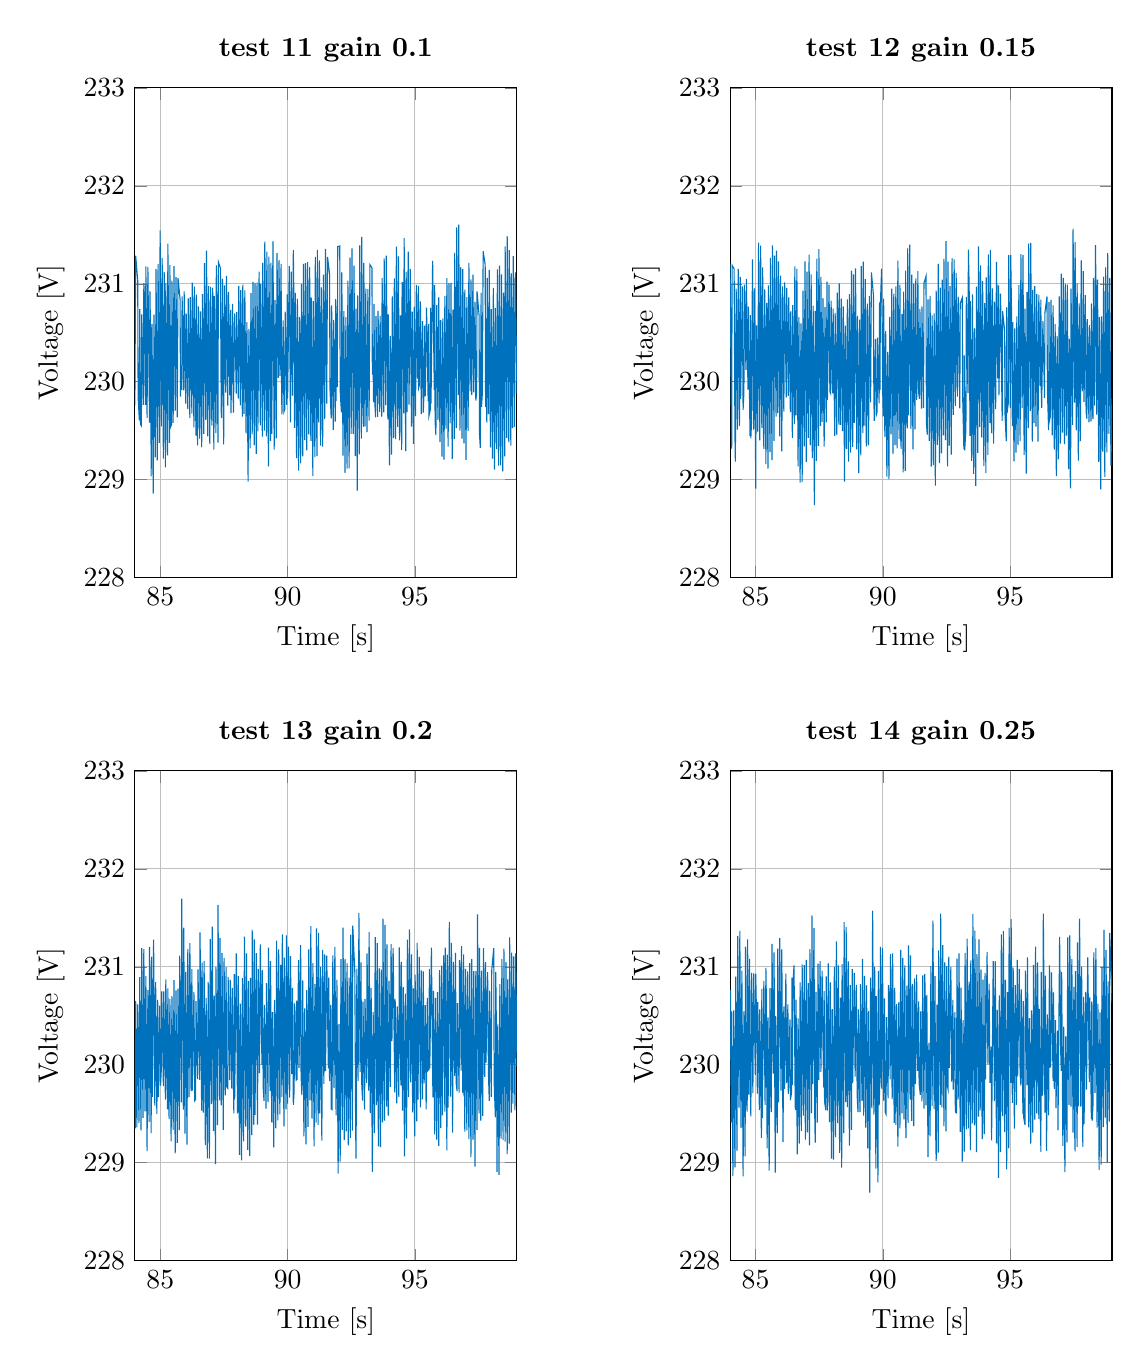
\begin{tikzpicture}

\begin{axis}[%
width=0.4\textwidth,
height=2.449in,
at={(1.024in,4.208in)},
scale only axis,
xmin=84,
xmax=99,
xlabel={Time [s]},
xmajorgrids,
ymin=228,
ymax=233,
ylabel={Voltage [V]},
ymajorgrids,
axis background/.style={fill=white},
title style={font=\bfseries},
title={test 11 gain 0.1}
]
\addplot [color=mycolor1,solid,forget plot]
  table[row sep=crcr]{%
84	229.759539348865\\
84.032	231.287255722638\\
84.112	231.034826347952\\
84.128	229.844375334181\\
84.176	229.60480560374\\
84.192	230.74148908202\\
84.224	229.564496318418\\
84.256	229.550690387856\\
84.272	230.688519623607\\
84.336	229.764744146321\\
84.352	231.005963576845\\
84.384	230.820846770409\\
84.416	229.76400141087\\
84.432	231.177508206234\\
84.48	229.632516104207\\
84.512	231.170660879894\\
84.576	229.582046347539\\
84.592	230.924983218894\\
84.624	230.33949264147\\
84.64	229.034729018478\\
84.672	230.59001564792\\
84.72	228.858811896569\\
84.752	230.684316846808\\
84.8	229.227898943224\\
84.832	231.150923417825\\
84.88	229.197334815695\\
84.912	231.20070204392\\
84.96	229.375593558492\\
84.992	231.544402831246\\
85.04	229.544306481839\\
85.072	231.265208418508\\
85.12	229.215153184104\\
85.152	231.119781113799\\
85.2	229.125555960708\\
85.216	231.005485117079\\
85.28	229.248351081836\\
85.296	231.409666853621\\
85.36	229.376036724189\\
85.376	231.191660584735\\
85.408	229.541276599794\\
85.44	229.562039267948\\
85.456	231.031812346774\\
85.504	229.581366380652\\
85.536	231.180614320727\\
85.584	229.70240768744\\
85.616	231.067136108227\\
85.664	229.637036909764\\
85.696	231.057456256167\\
85.776	230.841691134093\\
85.792	229.847621987007\\
85.824	230.171887543216\\
85.84	229.91776074848\\
85.856	230.87184389024\\
85.92	229.91137691611\\
85.936	230.921680690984\\
86	229.776601326446\\
86.016	230.695092533274\\
86.048	230.214398388446\\
86.08	229.719681346901\\
86.096	230.850063317386\\
86.16	229.627860821512\\
86.176	230.864628496094\\
86.24	229.674250671022\\
86.256	231.012241781408\\
86.32	229.533796626021\\
86.336	230.969928372629\\
86.4	229.449641309522\\
86.416	230.890040810824\\
86.464	229.350165361486\\
86.496	230.768160818134\\
86.544	229.42045988038\\
86.576	230.717682463064\\
86.624	229.331914832938\\
86.656	230.89413540657\\
86.704	229.468372055594\\
86.736	231.211911369353\\
86.784	229.60973723696\\
86.816	231.338206413398\\
86.848	229.767717129794\\
86.864	229.443482821504\\
86.896	230.976082263033\\
86.944	229.365717050751\\
86.976	230.969299380276\\
87.024	229.55165093391\\
87.056	230.959268101012\\
87.088	229.664502603923\\
87.104	229.30753835664\\
87.12	230.874862773081\\
87.184	229.474761552243\\
87.2	231.186860762503\\
87.216	230.855155433714\\
87.264	229.378978078114\\
87.28	231.222173845571\\
87.36	231.161218036408\\
87.392	229.689101995791\\
87.408	229.629699851067\\
87.44	231.050149247447\\
87.488	229.361881891101\\
87.504	230.24826866306\\
87.52	230.984032537672\\
87.568	229.887999368694\\
87.6	231.079686821515\\
87.648	229.755769222876\\
87.68	230.916335417452\\
87.728	229.860611895778\\
87.76	230.734535234949\\
87.776	229.679318061261\\
87.84	230.794470077645\\
87.856	229.985359403448\\
87.872	229.685087167184\\
87.92	230.698071841395\\
87.984	229.87927813557\\
88	230.714304682439\\
88.064	229.828368103769\\
88.08	230.97690367054\\
88.144	229.758365245771\\
88.16	230.935686102843\\
88.224	229.644530206311\\
88.24	230.992441092442\\
88.288	229.671241204489\\
88.32	230.933417998015\\
88.368	229.472215170185\\
88.4	230.609277335222\\
88.448	228.97977360109\\
88.464	229.957152639646\\
88.48	230.540722153158\\
88.528	229.320651835393\\
88.56	230.904277554716\\
88.608	229.462826374569\\
88.64	231.020165503811\\
88.688	229.352822430655\\
88.72	231.004902207144\\
88.768	229.263897286582\\
88.8	231.010723502078\\
88.832	229.494105630473\\
88.88	231.124889355417\\
88.928	229.554098769183\\
88.944	230.998903424512\\
89.008	229.439014431106\\
89.024	231.21385110468\\
89.088	229.501552305719\\
89.104	231.431368806669\\
89.168	229.442640043855\\
89.184	231.328205135738\\
89.248	229.136556425211\\
89.264	231.276143806256\\
89.328	229.395326747441\\
89.344	231.216913358541\\
89.376	229.466961716243\\
89.424	231.432517276344\\
89.472	229.307109973315\\
89.504	230.834609847081\\
89.552	229.422440523248\\
89.584	231.313063575666\\
89.632	230.038850234798\\
89.664	231.242554235791\\
89.696	230.060162143388\\
89.744	231.202414737847\\
89.76	230.01190443263\\
89.776	229.666448027988\\
89.824	230.625894393483\\
89.856	229.693175900921\\
89.888	229.717003039924\\
89.904	230.715355087663\\
89.968	229.764868590364\\
89.984	230.893050694478\\
90	229.830931398119\\
90.064	231.179338672004\\
90.112	229.585614396394\\
90.144	231.12453193215\\
90.192	229.859312015564\\
90.224	231.342571547677\\
90.256	230.619644426044\\
90.272	229.530003846914\\
90.304	230.907740470554\\
90.352	229.220736006179\\
90.384	230.847168967275\\
90.432	229.092512080193\\
90.464	230.659045051508\\
90.48	230.407682849046\\
90.512	229.166759769457\\
90.544	230.998104441579\\
90.592	229.238446288294\\
90.624	231.20432264862\\
90.672	229.403881879541\\
90.704	231.212194011863\\
90.752	229.299437897878\\
90.784	231.221145828582\\
90.832	229.463267610437\\
90.864	231.170952062735\\
90.912	229.395549766867\\
90.928	230.858376320351\\
90.992	229.035878876524\\
91.008	230.8217966359\\
91.072	229.230325457265\\
91.088	231.275840792302\\
91.152	229.24036381793\\
91.168	231.345503914212\\
91.216	229.586413472314\\
91.248	231.238084042073\\
91.296	229.349196022616\\
91.328	230.962192600942\\
91.36	229.844339047778\\
91.376	229.338374679393\\
91.408	231.092454094207\\
91.456	229.620830651994\\
91.488	231.356001402922\\
91.536	229.777704378472\\
91.568	231.274429876584\\
91.648	231.097178591034\\
91.664	229.927114291551\\
91.712	229.626446201151\\
91.728	230.778960713131\\
91.792	229.508765282889\\
91.808	230.63094890309\\
91.872	229.592059628317\\
91.888	230.844211069376\\
91.904	229.801835571184\\
91.92	230.700870334948\\
91.952	229.945041338954\\
91.968	231.379745150305\\
92.048	231.386407791167\\
92.064	229.910017765131\\
92.112	229.688271989445\\
92.128	231.11713377103\\
92.176	229.245207967982\\
92.208	230.720973241401\\
92.256	229.069546081666\\
92.288	230.660876646836\\
92.336	229.11310374146\\
92.368	231.031506186878\\
92.416	229.114588245951\\
92.448	231.268072067394\\
92.496	229.466804601895\\
92.528	231.362726295747\\
92.576	229.467147047684\\
92.608	231.184670660203\\
92.656	229.243346361412\\
92.688	230.747032223288\\
92.736	228.88958937419\\
92.752	230.881666058465\\
92.816	229.257953942446\\
92.832	231.391550190008\\
92.896	229.420499562918\\
92.912	231.479840677181\\
92.944	229.807576498441\\
92.976	229.540257430707\\
92.992	231.212790273935\\
93.04	229.545683995348\\
93.072	230.951740181534\\
93.088	230.024905911269\\
93.12	229.484625394301\\
93.152	230.9461584657\\
93.2	229.603218409591\\
93.232	231.195540088226\\
93.312	231.164199504568\\
93.328	230.073232388019\\
93.36	230.12616134308\\
93.376	229.792672343726\\
93.392	230.793723055933\\
93.424	229.787474400801\\
93.456	229.636151798113\\
93.472	230.671092618229\\
93.536	229.642501497825\\
93.552	230.723242893058\\
93.616	229.693018809922\\
93.632	230.672499475404\\
93.696	229.643195403781\\
93.712	231.06050377807\\
93.776	229.687202775277\\
93.792	231.25931553281\\
93.856	229.761081513104\\
93.872	231.28635080499\\
93.936	229.616991121684\\
93.952	230.687142946388\\
94	229.145891080523\\
94.032	230.467183155421\\
94.08	229.255517110041\\
94.096	230.041557612074\\
94.112	230.871893638964\\
94.16	229.424134558225\\
94.192	231.055256839474\\
94.24	229.41431495794\\
94.272	231.378176556963\\
94.32	229.539253008302\\
94.352	231.281074426641\\
94.384	229.706314150235\\
94.4	229.401852766635\\
94.432	230.676786864649\\
94.48	229.301120854913\\
94.496	231.012642257765\\
94.512	231.010072908227\\
94.56	229.678131534317\\
94.576	231.469700605431\\
94.64	229.292940493954\\
94.656	231.120359906941\\
94.688	229.690438484462\\
94.736	231.329358580068\\
94.752	230.494255303834\\
94.768	229.766328130271\\
94.816	231.152973815076\\
94.864	229.541384819959\\
94.896	230.716698591168\\
94.944	229.366935478867\\
94.976	230.765651252356\\
95.024	229.648873975773\\
95.056	230.989884660203\\
95.104	230.032795431026\\
95.136	230.979378551875\\
95.152	229.940814063626\\
95.168	229.95796818703\\
95.216	230.821421867299\\
95.248	229.668778528308\\
95.296	230.619772685284\\
95.328	229.684615945737\\
95.36	229.908229500462\\
95.376	230.571624594187\\
95.408	229.849974893888\\
95.456	230.756300300207\\
95.52	229.79955618323\\
95.536	230.590905587481\\
95.552	229.651785202548\\
95.6	229.707500966074\\
95.616	230.753975645828\\
95.632	229.777737891673\\
95.696	231.234974865265\\
95.76	229.917912901242\\
95.776	230.9863300682\\
95.792	229.599206770543\\
95.824	229.454497324694\\
95.856	230.783341426378\\
95.904	229.611363842771\\
95.936	230.862377101305\\
95.984	229.386580070626\\
96.016	230.62977563849\\
96.064	229.23630710005\\
96.096	230.647305342608\\
96.144	229.204328706469\\
96.176	230.873748102789\\
96.224	229.522337220196\\
96.256	231.057249662634\\
96.304	229.336805219708\\
96.336	231.007452187379\\
96.384	229.575012553661\\
96.4	230.251073724219\\
96.416	231.009762096354\\
96.464	229.210798469746\\
96.496	230.737487346569\\
96.544	229.413804868152\\
96.56	231.314401740594\\
96.624	229.527808555798\\
96.64	231.575259485647\\
96.704	229.862682818207\\
96.72	231.603241118857\\
96.768	229.501486699569\\
96.8	231.167589369044\\
96.848	229.418260903852\\
96.88	231.149734724149\\
96.928	229.370735980885\\
96.96	230.940757852609\\
96.992	229.722467077727\\
97.008	229.203301339133\\
97.04	230.864585357423\\
97.088	229.497777387489\\
97.12	231.213377202751\\
97.168	229.902799351665\\
97.2	231.045734050924\\
97.232	229.866127202685\\
97.28	231.093620055629\\
97.312	229.891701510836\\
97.36	230.814731011776\\
97.392	229.806885146337\\
97.424	229.888441839159\\
97.44	230.922886502044\\
97.52	230.676705593902\\
97.536	229.467532103735\\
97.568	229.325909459444\\
97.6	230.906981921114\\
97.616	229.742516256509\\
97.648	229.876354645602\\
97.68	231.332929301367\\
97.76	231.193931295874\\
97.776	229.7404421541\\
97.792	230.646022705177\\
97.824	229.582518772568\\
97.84	231.061259722924\\
97.888	229.670484000027\\
97.92	231.143126574106\\
97.968	229.3310291673\\
98	230.740736300038\\
98.048	229.216245251691\\
98.08	230.958807562093\\
98.128	229.10251590668\\
98.16	230.752936868009\\
98.208	229.311016365645\\
98.24	231.147529998616\\
98.288	229.142851951825\\
98.32	231.184308062864\\
98.368	229.146369135551\\
98.4	231.095954298043\\
98.448	229.085594355521\\
98.48	230.909016040444\\
98.528	229.239352047557\\
98.544	231.38112114891\\
98.608	229.425962499112\\
98.624	231.48694129223\\
98.688	229.381808132135\\
98.704	231.343362605547\\
98.768	229.348572156816\\
98.784	231.107302525525\\
98.832	229.525532142822\\
98.864	231.281734767395\\
98.912	229.538145926157\\
98.944	231.11619210373\\
99.008	229.882591215438\\
};
\end{axis}

\begin{axis}[%
width=0.4\textwidth,
height=2.449in,
at={(4in,4.208in)},
scale only axis,
xmin=84,
xmax=99,
xlabel={Time [s]},
xmajorgrids,
ymin=228,
ymax=233,
ylabel={Voltage [V]},
ymajorgrids,
axis background/.style={fill=white},
title style={font=\bfseries},
title={test 12  gain 0.15}
]
\addplot [color=mycolor1,solid,forget plot]
  table[row sep=crcr]{%
84	231.207695384205\\
84.064	229.316641640256\\
84.08	231.188435898942\\
84.16	231.152951313325\\
84.192	229.447993374027\\
84.208	229.185268435007\\
84.24	230.950054303124\\
84.288	229.512351627222\\
84.32	231.153370140871\\
84.368	229.548228442274\\
84.4	231.069296329452\\
84.416	229.82422388058\\
84.48	230.974287270437\\
84.512	229.71341367411\\
84.544	229.891658268851\\
84.56	230.991791230368\\
84.624	230.122387762045\\
84.64	231.049652788206\\
84.704	229.920762904306\\
84.72	230.766814248675\\
84.784	229.444985537726\\
84.8	230.680954581019\\
84.816	229.422080195165\\
84.848	229.61487830343\\
84.88	231.250024497241\\
84.928	229.511406510272\\
84.96	230.952356959041\\
85.008	228.908671209741\\
85.024	229.942055222944\\
85.04	230.575598701667\\
85.088	229.490327287371\\
85.12	231.420828161362\\
85.168	229.401780681061\\
85.2	231.389866084937\\
85.248	229.528153326259\\
85.28	231.166532214251\\
85.312	229.457194748221\\
85.328	229.315820388439\\
85.36	230.943726957409\\
85.408	229.158186132556\\
85.424	230.514229597335\\
85.44	230.806131370949\\
85.488	229.11305379768\\
85.504	230.982982966535\\
85.568	229.281836226181\\
85.584	231.265199116681\\
85.648	229.201079002688\\
85.664	231.391708161694\\
85.728	229.39679570835\\
85.744	231.288311152317\\
85.808	229.645092314808\\
85.824	231.33888872863\\
85.872	229.679139531845\\
85.904	231.228868278743\\
85.952	229.442471501558\\
85.984	231.082766229309\\
86.032	229.288613724172\\
86.064	230.97311793393\\
86.112	229.694595191781\\
86.144	231.013185827748\\
86.208	229.839474384189\\
86.224	230.958748204974\\
86.288	229.856977659307\\
86.304	230.862233948835\\
86.368	229.689338051202\\
86.384	230.719511779797\\
86.448	229.42725427859\\
86.464	230.782448696901\\
86.528	229.567192916303\\
86.544	231.177296638441\\
86.592	229.658015736067\\
86.624	231.151632486074\\
86.672	229.13686962403\\
86.704	230.659820012983\\
86.752	228.971083341178\\
86.784	230.596467178734\\
86.8	230.308793740868\\
86.832	228.976217941071\\
86.864	230.929667325508\\
86.912	229.339902228968\\
86.944	231.229936658127\\
86.992	229.181611629536\\
87.024	231.124199112152\\
87.04	230.330270605998\\
87.072	229.428264425603\\
87.104	231.298820635285\\
87.152	229.350273905128\\
87.184	231.096933778634\\
87.232	229.219632179082\\
87.264	230.775930039916\\
87.312	228.740455760544\\
87.344	230.724196054524\\
87.392	229.193320249151\\
87.408	231.256679808048\\
87.472	229.345408981973\\
87.488	231.353125488602\\
87.552	229.549558980739\\
87.568	231.070053108784\\
87.616	229.590629617322\\
87.648	230.854476985927\\
87.68	229.727721081553\\
87.696	229.337992749224\\
87.728	230.762071127386\\
87.776	229.584909606204\\
87.808	231.023070682037\\
87.824	229.812338058133\\
87.888	230.990758371077\\
87.92	229.899616076642\\
87.952	229.879245521815\\
87.968	230.829174635567\\
88.032	229.88177742568\\
88.048	230.746480083237\\
88.096	229.777761305405\\
88.112	229.447509295687\\
88.128	230.704245957691\\
88.192	229.4600176238\\
88.208	230.910173079213\\
88.24	230.654082709714\\
88.272	229.562973299667\\
88.288	231.003884616242\\
88.336	229.560264191828\\
88.368	230.847436896982\\
88.416	229.495517055179\\
88.448	230.768918249412\\
88.464	230.316689182673\\
88.496	228.979439407442\\
88.528	230.573494894536\\
88.576	229.31397358761\\
88.608	230.841324148198\\
88.656	229.183380529725\\
88.688	230.89372354469\\
88.736	229.27646521698\\
88.768	231.133753566543\\
88.816	229.336029779913\\
88.848	231.09652018837\\
88.88	229.580144018684\\
88.928	231.157929629047\\
88.976	229.310125054222\\
89.008	230.672391294347\\
89.056	229.06643315028\\
89.088	230.6335249784\\
89.136	229.247635769938\\
89.152	231.180981271501\\
89.216	229.476258406229\\
89.232	231.225171059474\\
89.264	229.552623889337\\
89.312	231.04761361662\\
89.344	229.414767880479\\
89.36	229.341028015494\\
89.392	230.797370015631\\
89.44	229.3537061122\\
89.472	230.873799882855\\
89.52	229.789314986503\\
89.552	231.117136814428\\
89.632	230.883378013801\\
89.648	229.84194012928\\
89.664	229.601275186557\\
89.68	229.951127845424\\
89.712	230.436046857657\\
89.744	229.662646000328\\
89.776	229.692267393481\\
89.792	230.450419048799\\
89.856	229.778378679216\\
89.872	230.809265102888\\
89.888	229.917368087388\\
89.904	230.783158095136\\
89.952	231.154555550519\\
90	229.839247318581\\
90.016	229.645443931026\\
90.032	230.848992841109\\
90.08	229.435061960107\\
90.112	230.516770826891\\
90.16	229.030863615765\\
90.192	230.306054145306\\
90.24	229.004821140702\\
90.272	230.663181782346\\
90.32	229.461677234916\\
90.352	230.949423555966\\
90.4	229.26709093008\\
90.432	230.89888144883\\
90.48	229.353996127301\\
90.512	230.974460232567\\
90.56	229.320538470312\\
90.592	231.236698734202\\
90.64	229.416167842584\\
90.672	230.987828227048\\
90.704	229.413350424833\\
90.72	229.315768198551\\
90.752	230.690275389899\\
90.8	229.074276829315\\
90.816	230.920750182736\\
90.88	229.087883424357\\
90.896	231.134160293565\\
90.928	229.620645262073\\
90.96	229.523976191797\\
90.976	231.361334015374\\
91.008	229.657040991056\\
91.056	231.399038898399\\
91.072	230.378430940673\\
91.104	229.519242419536\\
91.136	231.094741119441\\
91.184	229.308726903146\\
91.216	231.001603217056\\
91.264	229.514764700982\\
91.296	231.055140396742\\
91.328	229.816275220155\\
91.36	230.097795781343\\
91.376	231.131060282631\\
91.408	229.88983470459\\
91.44	229.826144654767\\
91.456	230.743387913154\\
91.52	229.72678935743\\
91.536	230.76956357556\\
91.6	229.733243492326\\
91.616	231.004996500215\\
91.696	231.076563071715\\
91.712	229.581939917234\\
91.744	229.461171513299\\
91.776	230.841547277288\\
91.824	229.396734566781\\
91.856	230.877623393081\\
91.904	229.134086059472\\
91.936	230.678383817505\\
91.984	229.149929482502\\
92.016	230.698839403749\\
92.064	228.940586906448\\
92.096	230.928927075651\\
92.128	229.838095682994\\
92.144	229.355707745642\\
92.176	231.203466090198\\
92.224	229.169570730918\\
92.256	230.96148973231\\
92.304	229.269992729842\\
92.336	231.043557012157\\
92.368	229.774163261642\\
92.384	229.452141882041\\
92.4	231.25348261323\\
92.464	229.403422351042\\
92.48	231.436203358232\\
92.496	230.770693801079\\
92.544	229.136212183175\\
92.56	231.227327230145\\
92.608	229.347474461019\\
92.64	230.976630914063\\
92.688	229.256348599812\\
92.72	231.262598189776\\
92.768	229.662291925102\\
92.784	230.288307105557\\
92.8	231.249336699949\\
92.848	229.752788033954\\
92.88	231.110401013836\\
92.928	229.848344599545\\
92.96	230.868683419422\\
93.024	229.727418942176\\
93.04	230.801166490026\\
93.12	230.8559768197\\
93.136	229.852995745681\\
93.184	229.312338233907\\
93.2	230.270009278033\\
93.216	229.300020227654\\
93.264	229.510536766115\\
93.28	230.866836245724\\
93.344	229.88352391291\\
93.36	231.348384931151\\
93.392	230.957577076565\\
93.424	229.448443600443\\
93.44	230.823484588942\\
93.488	229.191074909181\\
93.504	229.534684714436\\
93.52	230.89254949621\\
93.568	229.060360697932\\
93.6	230.54441439003\\
93.648	228.937601172948\\
93.68	230.971358949885\\
93.728	229.273281157755\\
93.76	231.382044963248\\
93.792	229.993619326468\\
93.808	229.536874252359\\
93.84	231.187067500611\\
93.888	229.429664411503\\
93.92	231.029422775894\\
93.968	229.140548966502\\
94	230.802050826237\\
94.048	229.068124504649\\
94.064	231.066374086442\\
94.128	229.253068250186\\
94.144	231.299690780281\\
94.208	229.57675284557\\
94.224	231.344902799862\\
94.272	229.476630065936\\
94.304	230.952275690949\\
94.352	229.367915057769\\
94.384	230.816704896313\\
94.432	229.722556555918\\
94.464	231.223646988406\\
94.512	230.035570464347\\
94.544	230.983732561715\\
94.56	229.86038307657\\
94.624	230.899680483534\\
94.688	229.599968495154\\
94.704	230.720616788985\\
94.784	230.522926008693\\
94.8	229.663865514446\\
94.848	229.393330563544\\
94.864	230.75896196301\\
94.88	229.677969105564\\
94.928	229.782826622735\\
94.944	231.292424347447\\
95.008	229.731604205416\\
95.024	231.292659706269\\
95.056	230.697056213367\\
95.088	229.547404381544\\
95.104	230.60894761783\\
95.152	229.186651484039\\
95.168	229.587611792046\\
95.184	230.544935533866\\
95.232	229.275271757906\\
95.264	230.668494192193\\
95.312	229.35352136649\\
95.344	230.986004642845\\
95.392	229.394145140575\\
95.424	231.302743360195\\
95.472	229.733957939682\\
95.504	231.292652575904\\
95.552	229.251441814502\\
95.568	230.198247785666\\
95.584	230.747516466663\\
95.632	229.061943745118\\
95.664	230.915896938992\\
95.712	229.527410510789\\
95.728	231.410974870152\\
95.792	229.699912803438\\
95.808	231.418790495913\\
95.872	229.389506747856\\
95.888	230.936639731329\\
95.936	229.577524588559\\
95.968	230.975582690697\\
96.016	229.540670453646\\
96.048	230.896826122044\\
96.096	229.388450912664\\
96.128	230.887798049451\\
96.176	229.956316332999\\
96.208	230.838173239818\\
96.224	229.892304516313\\
96.24	229.734512992154\\
96.288	230.617641386336\\
96.352	229.835476430841\\
96.368	230.70698056513\\
96.448	230.869731889002\\
96.464	229.91436732872\\
96.512	229.507459813417\\
96.528	230.813934354172\\
96.544	229.599987804671\\
96.576	229.640445412216\\
96.608	230.837887654172\\
96.656	229.452203233012\\
96.688	230.779185008617\\
96.736	229.308375120744\\
96.768	230.588328908882\\
96.816	229.036388155587\\
96.848	230.467313779654\\
96.896	229.206424289652\\
96.928	230.870369261882\\
96.944	230.602274004054\\
96.976	229.368055466716\\
97.008	231.103904316107\\
97.056	229.479821907403\\
97.088	231.061261566466\\
97.136	229.36316664074\\
97.168	230.998955444327\\
97.216	229.449515045391\\
97.232	230.345453068088\\
97.248	230.991920390949\\
97.296	229.107910691797\\
97.328	230.43886462312\\
97.36	229.060723662252\\
97.376	228.910697386581\\
97.392	230.950216524997\\
97.456	229.560647543455\\
97.472	231.560223996186\\
97.536	229.78759666562\\
97.552	231.424415248472\\
97.6	229.504339931435\\
97.632	231.004132101381\\
97.68	229.195806843458\\
97.712	230.800303332435\\
97.76	229.393208328238\\
97.792	231.238448136319\\
97.808	230.071430867682\\
97.84	229.90178812666\\
97.872	231.130292072838\\
97.904	229.790948907635\\
97.952	230.883669369046\\
97.984	229.694780425019\\
98.016	229.621383107668\\
98.032	230.639200002557\\
98.096	229.584730228672\\
98.112	230.577252239296\\
98.176	229.596508716084\\
98.192	230.798743509437\\
98.24	229.667389968331\\
98.256	229.619835497292\\
98.272	231.057164490672\\
98.32	229.755965146106\\
98.352	231.395238480009\\
98.384	230.703825780986\\
98.4	229.66462785481\\
98.432	231.042843148307\\
98.48	229.181036807683\\
98.512	230.658408612494\\
98.56	228.902121335737\\
98.592	230.668170920869\\
98.608	230.473768519753\\
98.64	229.286300453457\\
98.672	231.072368684649\\
98.72	229.02957705765\\
98.752	231.166759597059\\
98.8	229.27849900469\\
98.832	231.312118881447\\
98.88	229.469139961019\\
98.912	231.060521457659\\
98.96	229.14403449003\\
99.008	229.827899327049\\
};
\end{axis}

\begin{axis}[%
width=0.4\textwidth,
height=2.449in,
at={(1.024in,0.793in)},
scale only axis,
xmin=84,
xmax=99,
xlabel={Time [s]},
xmajorgrids,
ymin=228,
ymax=233,
ylabel={Voltage [V]},
ymajorgrids,
axis background/.style={fill=white},
title style={font=\bfseries},
title={test 13  gain 0.2}
]
\addplot [color=mycolor1,solid,forget plot]
  table[row sep=crcr]{%
84	229.507423535777\\
84.016	229.350984746219\\
84.032	230.651246580127\\
84.08	229.361470082815\\
84.112	230.61537288611\\
84.16	229.405931246136\\
84.192	230.893296220765\\
84.24	229.331130722532\\
84.272	231.189777066918\\
84.32	229.458168755739\\
84.352	231.180109068454\\
84.4	229.52392442222\\
84.416	230.129940052337\\
84.432	230.905622757479\\
84.48	229.119307819682\\
84.512	230.761495857782\\
84.56	229.416682353498\\
84.576	231.199518405112\\
84.64	229.302820488936\\
84.656	231.103646643218\\
84.688	229.673026487813\\
84.736	231.276046812803\\
84.784	229.583091477338\\
84.816	230.844246746694\\
84.864	229.497427886541\\
84.896	230.662794343332\\
84.928	229.669918127102\\
84.976	230.604057298127\\
85.008	229.786569978396\\
85.04	229.952090313357\\
85.056	230.749197727435\\
85.12	229.784191693675\\
85.136	230.749930940934\\
85.2	229.642846427745\\
85.216	230.871136848516\\
85.28	229.543577990137\\
85.296	230.779313515235\\
85.344	229.445343944775\\
85.376	230.670908818313\\
85.424	229.216768155424\\
85.456	230.701295750006\\
85.504	229.335047225891\\
85.536	230.86412178023\\
85.584	229.09569925241\\
85.616	230.759767081756\\
85.664	229.20349097719\\
85.696	230.777588359075\\
85.744	229.33226825597\\
85.76	231.112836774325\\
85.824	229.616374019978\\
85.84	231.695068412408\\
85.904	229.541917605993\\
85.92	231.398513087166\\
85.968	229.29669262215\\
86	230.947310883375\\
86.048	229.183851726045\\
86.08	231.179036137433\\
86.128	229.67070098289\\
86.16	231.24042012586\\
86.208	229.731237354052\\
86.24	230.975199307729\\
86.256	229.73657926514\\
86.32	230.740054460557\\
86.352	229.633625889197\\
86.384	229.644792451376\\
86.4	230.648442414851\\
86.464	229.853208542477\\
86.48	230.974197967188\\
86.544	229.846118292237\\
86.56	231.351226923257\\
86.624	229.531604991974\\
86.64	231.042206860337\\
86.688	229.511287149007\\
86.72	231.061277670648\\
86.768	229.180477118483\\
86.8	230.683701790715\\
86.848	229.044284517408\\
86.88	230.844352153251\\
86.928	229.040715498517\\
86.96	231.283303722737\\
87.008	229.598385681684\\
87.04	231.410283686323\\
87.088	229.324940859035\\
87.12	230.706000317465\\
87.168	228.986506656676\\
87.184	231.000297367769\\
87.248	229.384449705723\\
87.264	231.632567600969\\
87.328	229.637187136571\\
87.344	231.295208893329\\
87.392	229.585447842384\\
87.424	231.142386833612\\
87.472	229.335183321981\\
87.504	231.092003891799\\
87.552	229.688365418015\\
87.584	230.995545409544\\
87.6	229.7782890562\\
87.648	229.761040503203\\
87.664	230.897035179869\\
87.728	229.842811515232\\
87.744	230.867911558788\\
87.808	229.757303940917\\
87.824	230.785584906837\\
87.888	229.503322459251\\
87.904	230.926320244894\\
87.92	229.645407454076\\
87.984	231.135943176144\\
88.032	229.503971996567\\
88.048	229.531274098409\\
88.064	230.905103222378\\
88.112	229.078945902531\\
88.144	230.624591612622\\
88.192	229.024257601846\\
88.224	230.883690470748\\
88.272	229.217090996093\\
88.304	231.308777658337\\
88.352	229.36877974321\\
88.384	231.136680979166\\
88.432	229.130871064399\\
88.464	230.855695404318\\
88.512	229.069646427519\\
88.544	230.886620815365\\
88.592	229.281391503775\\
88.608	231.376677050261\\
88.672	229.385008578163\\
88.688	231.279496297875\\
88.72	229.489337738929\\
88.768	231.139605865911\\
88.816	229.388039711653\\
88.848	230.979243128528\\
88.896	229.913822106984\\
88.928	231.229794748045\\
88.992	229.999961100398\\
89.008	230.9656756773\\
89.04	229.77163816826\\
89.072	229.630552550082\\
89.088	230.611182920801\\
89.152	229.552528127796\\
89.168	230.83366550211\\
89.232	229.61876131554\\
89.248	231.194691779324\\
89.312	229.732311231385\\
89.328	231.058859953365\\
89.376	229.412139790885\\
89.408	230.537257564234\\
89.456	229.156021759897\\
89.472	229.974856932501\\
89.488	230.662389427893\\
89.536	229.350587028999\\
89.568	231.26582676967\\
89.616	229.4309639361\\
89.648	231.176851497545\\
89.696	229.492765528477\\
89.728	231.019641060506\\
89.776	229.670412246767\\
89.792	231.329686812198\\
89.856	229.371058541159\\
89.872	231.092589004903\\
89.888	230.607456506512\\
89.936	229.545587337424\\
89.952	231.319951392282\\
90	229.602304518328\\
90.032	231.204977010777\\
90.08	229.665046429825\\
90.112	231.109328005543\\
90.16	229.905485723781\\
90.192	230.784402316062\\
90.224	229.590690193593\\
90.256	229.72579526158\\
90.272	230.626287659399\\
90.336	229.833126501166\\
90.352	230.655052120151\\
90.368	229.846105850507\\
90.432	231.068044235858\\
90.448	229.965285802206\\
90.512	231.220587522239\\
90.528	229.896004715931\\
90.56	229.689653124984\\
90.592	230.861414885574\\
90.64	229.268391835562\\
90.656	229.909617638226\\
90.672	230.576537734492\\
90.72	229.187801278837\\
90.752	230.762862948747\\
90.8	229.365842141247\\
90.832	231.178171629597\\
90.88	229.636623934754\\
90.912	231.414124034967\\
90.944	229.745856276021\\
90.96	229.449029913189\\
90.992	231.038590058745\\
91.04	229.167801315239\\
91.072	230.822570752317\\
91.12	229.409274510489\\
91.136	231.391614291852\\
91.2	229.387263430185\\
91.216	231.344929755086\\
91.264	229.503563031758\\
91.296	230.999329130204\\
91.344	229.22659563709\\
91.36	230.091268283826\\
91.376	231.172128477892\\
91.424	229.805839816056\\
91.456	231.125563539166\\
91.488	229.933958753338\\
91.536	231.114768141096\\
91.6	229.964240373881\\
91.616	230.888315419352\\
91.648	229.833687826264\\
91.696	230.611313208686\\
91.712	229.549000724218\\
91.744	229.542589634006\\
91.776	231.115742168383\\
91.824	229.761704808915\\
91.856	231.203423701325\\
91.904	229.483759450474\\
91.936	230.866715361321\\
91.984	228.88808721815\\
92.016	230.414772470446\\
92.064	229.011050216683\\
92.096	231.077031434493\\
92.128	229.978132747436\\
92.144	229.334541436367\\
92.176	231.39877471909\\
92.224	229.230024848569\\
92.256	231.076972899564\\
92.304	229.320217782151\\
92.336	231.034574081911\\
92.368	229.560713561194\\
92.384	229.17750587385\\
92.416	230.889777850633\\
92.464	229.252714180354\\
92.48	231.328562522994\\
92.496	230.874662675728\\
92.544	229.327445397254\\
92.56	231.419022798496\\
92.64	230.936684291932\\
92.672	229.337719546893\\
92.688	229.041598461801\\
92.72	230.980490251753\\
92.768	229.834492306334\\
92.784	230.515321447508\\
92.8	231.550398603187\\
92.848	229.927966762641\\
92.88	231.04421775122\\
92.912	229.801763380347\\
92.944	229.63366435327\\
92.96	230.643484290962\\
93.024	229.540721859075\\
93.04	230.672579458188\\
93.104	229.814803242131\\
93.12	231.138135299826\\
93.184	229.736456164645\\
93.2	231.35455365816\\
93.248	229.504949995364\\
93.28	230.781021048027\\
93.328	228.90624688404\\
93.36	230.536993859123\\
93.408	229.30339802523\\
93.44	231.304049434712\\
93.488	229.586634843427\\
93.52	231.242505088874\\
93.552	229.614935474072\\
93.568	229.167405930016\\
93.6	230.984800881677\\
93.648	229.15911061379\\
93.68	230.970723817508\\
93.728	229.412498564707\\
93.744	231.491488198492\\
93.776	230.068260978875\\
93.808	229.428480633623\\
93.824	231.428908029648\\
93.888	229.573075055357\\
93.904	231.227634870758\\
93.92	230.173345618997\\
93.952	229.479594810729\\
93.984	230.855103645474\\
94.032	229.774116206409\\
94.064	231.231201215533\\
94.096	230.24010485272\\
94.144	231.1937444487\\
94.208	229.71807237922\\
94.224	230.666383473656\\
94.288	229.606060911365\\
94.304	230.596046784267\\
94.368	229.672206696799\\
94.384	231.198796392994\\
94.448	229.788520735192\\
94.464	231.051201808956\\
94.512	229.531831965779\\
94.544	230.792167098514\\
94.592	229.064025904362\\
94.624	230.726832581564\\
94.672	229.245835345036\\
94.704	231.276052467289\\
94.752	229.670673172875\\
94.784	231.382138115811\\
94.832	229.820594428095\\
94.864	231.126208041507\\
94.912	229.513966523275\\
94.944	230.778374220237\\
94.976	229.603112132957\\
94.992	229.268987003178\\
95.008	230.918858961774\\
95.072	229.421622713258\\
95.088	231.24323391796\\
95.12	229.643814107848\\
95.168	231.101471840134\\
95.216	229.56374521973\\
95.248	230.964011579595\\
95.296	229.645337423453\\
95.328	230.95354031676\\
95.36	229.809676380863\\
95.376	229.930864179324\\
95.408	230.608741363919\\
95.44	229.545495372018\\
95.488	230.683711089374\\
95.504	229.9397331406\\
95.552	229.953736982956\\
95.568	230.978723428543\\
95.584	229.965170793936\\
95.648	231.196780733553\\
95.696	229.863034709427\\
95.712	229.665937673374\\
95.728	230.754972007643\\
95.776	229.290367200224\\
95.808	230.683531336338\\
95.856	229.236024429516\\
95.888	230.740515163701\\
95.936	229.172558261851\\
95.968	230.966443409755\\
96.016	229.354812600131\\
96.048	231.013078765786\\
96.08	229.483638041334\\
96.128	231.117516541548\\
96.176	229.520321819525\\
96.192	231.194923810425\\
96.256	229.126900097904\\
96.272	231.123403996168\\
96.304	229.562018095182\\
96.352	231.456903799261\\
96.4	229.674637622122\\
96.432	231.24456447653\\
96.48	229.30647126804\\
96.512	231.0498958377\\
96.56	229.885539611984\\
96.576	230.107775796163\\
96.592	231.141322454744\\
96.624	229.805720866828\\
96.656	229.731344958928\\
96.672	230.629871167043\\
96.736	229.714366556613\\
96.752	231.068418691945\\
96.784	230.928825592047\\
96.816	229.940413750241\\
96.832	231.211736083281\\
96.88	229.723842609375\\
96.896	229.709065586847\\
96.912	231.127187402434\\
96.96	229.317198188872\\
96.992	230.978493035616\\
97.04	229.329312132691\\
97.072	230.95328042973\\
97.12	229.24027101\\
97.152	231.038437132257\\
97.2	229.056425772164\\
97.232	231.07946204865\\
97.28	229.236357519459\\
97.312	230.954472196926\\
97.36	228.960048900393\\
97.392	230.954753204368\\
97.44	229.334592397065\\
97.456	231.534326454722\\
97.52	229.503424056271\\
97.536	231.193586058896\\
97.584	229.42934685075\\
97.6	229.850161291147\\
97.616	230.960287869765\\
97.664	229.475390564643\\
97.696	231.190104562615\\
97.744	229.875248654972\\
97.776	231.046579165564\\
97.792	230.020507702541\\
97.856	230.945550737576\\
97.888	229.91249069892\\
97.92	229.630682210721\\
97.936	230.755439153639\\
97.968	230.149138018865\\
98	229.67306663824\\
98.016	230.961078439021\\
98.096	231.191501407819\\
98.112	229.823084966411\\
98.16	229.463602029056\\
98.176	230.948814679253\\
98.208	230.171921708242\\
98.224	228.905849233786\\
98.256	230.411137546361\\
98.304	228.875265231623\\
98.336	230.823991428291\\
98.384	229.244729406932\\
98.416	231.080539555378\\
98.464	229.229449821815\\
98.496	231.184324345752\\
98.544	229.214691388421\\
98.576	231.048841495464\\
98.624	229.088058462698\\
98.64	230.871875492105\\
98.704	229.195019412899\\
98.72	231.2992797137\\
98.784	229.512521437028\\
98.8	231.145819922783\\
98.848	229.603841214292\\
98.88	231.107428884346\\
98.928	229.535970764151\\
98.96	231.137126323089\\
99.008	229.982443686319\\
};
\end{axis}

\begin{axis}[%
width=0.4\textwidth,
height=2.449in,
at={(4in,0.793in)},
scale only axis,
xmin=84,
xmax=99,
xlabel={Time [s]},
xmajorgrids,
ymin=228,
ymax=233,
ylabel={Voltage [V]},
ymajorgrids,
axis background/.style={fill=white},
title style={font=\bfseries},
title={test 14  gain 0.25}
]
\addplot [color=mycolor1,solid,forget plot]
  table[row sep=crcr]{%
84	230.053192238768\\
84.016	230.760754398474\\
84.048	229.411054657579\\
84.064	230.543705682979\\
84.112	228.862649367873\\
84.144	230.553816238179\\
84.192	228.952124682529\\
84.224	230.899965603523\\
84.272	229.123011005659\\
84.304	231.316457325498\\
84.352	229.562578799705\\
84.384	231.366788123778\\
84.416	229.809087464395\\
84.432	229.353069257124\\
84.464	230.961169204129\\
84.512	228.859833511835\\
84.544	230.546041891654\\
84.592	229.065314626565\\
84.608	231.205646465797\\
84.64	229.659454583413\\
84.672	229.52139928231\\
84.688	231.280079592364\\
84.736	229.695695651901\\
84.768	231.080407748017\\
84.784	230.038649511322\\
84.816	229.473369482309\\
84.848	230.937398403104\\
84.896	229.709273752253\\
84.928	230.933508328288\\
84.992	229.896976515768\\
85.008	230.928685356433\\
85.056	230.257601934376\\
85.072	229.70412046557\\
85.088	230.638846808873\\
85.152	229.537378550864\\
85.168	230.565560929509\\
85.232	229.252644069379\\
85.248	230.773441837303\\
85.264	229.457415852564\\
85.328	230.855313106155\\
85.376	229.591064648888\\
85.408	230.990129346918\\
85.424	230.692150868975\\
85.456	229.147215534213\\
85.488	230.482869865419\\
85.536	228.918481405486\\
85.568	230.781589924986\\
85.616	229.51572412362\\
85.648	231.233317651854\\
85.696	229.908510646934\\
85.728	231.147738211264\\
85.776	228.898780832401\\
85.792	230.498768437802\\
85.824	229.55458522944\\
85.856	229.302043621727\\
85.872	231.184743808176\\
85.904	229.616877978821\\
85.952	231.291447112999\\
86	229.736105211902\\
86.032	231.178291311136\\
86.08	229.20983715261\\
86.112	230.596073385122\\
86.144	229.754061026414\\
86.192	230.93088968461\\
86.224	229.814848489435\\
86.24	230.231911123029\\
86.272	230.617362914679\\
86.288	229.703130296966\\
86.352	230.462273276737\\
86.368	229.638180400952\\
86.416	229.714959761678\\
86.432	230.889653725199\\
86.448	229.793644327816\\
86.464	230.787107953244\\
86.512	231.015341918528\\
86.56	229.568632094681\\
86.576	229.537696397873\\
86.592	230.665083988645\\
86.64	229.085488343442\\
86.672	230.474558813121\\
86.72	229.194152243949\\
86.752	230.842093135214\\
86.8	229.32600096967\\
86.832	231.025457351371\\
86.88	229.479713642227\\
86.912	231.015991325367\\
86.96	229.234573912002\\
86.992	231.069538895401\\
87.04	229.309289921264\\
87.072	230.833065400271\\
87.12	229.177377874185\\
87.136	231.181545443412\\
87.2	229.506757406227\\
87.216	231.525017573987\\
87.248	229.80167452637\\
87.296	231.393775971911\\
87.328	229.460501475762\\
87.344	229.204455052839\\
87.376	230.743625935736\\
87.424	229.410327444492\\
87.456	231.032064387027\\
87.488	229.845869204032\\
87.536	231.058362902606\\
87.568	229.92639762107\\
87.616	230.960554138693\\
87.648	230.204111147032\\
87.68	229.769958279044\\
87.696	230.75208002296\\
87.712	229.622961320858\\
87.76	229.538318811391\\
87.776	230.903300031857\\
87.824	229.531613107573\\
87.856	231.034923060871\\
87.904	229.41465001074\\
87.936	230.841558047753\\
87.984	229.041825926017\\
88.016	230.567383720021\\
88.064	229.03192962368\\
88.096	230.998578841994\\
88.144	229.261562211519\\
88.176	231.26048092848\\
88.224	229.403352938473\\
88.256	231.013427425672\\
88.304	229.100973356792\\
88.336	230.684121172595\\
88.384	228.949077321829\\
88.4	231.02763856653\\
88.464	229.301333561649\\
88.48	231.455924651269\\
88.544	229.617276359225\\
88.56	231.406733810441\\
88.608	229.568298907235\\
88.64	231.056266662538\\
88.688	229.174575292602\\
88.72	230.813352083625\\
88.768	229.336176409949\\
88.8	230.978635880906\\
88.816	229.813519531429\\
88.88	230.937393885469\\
88.912	229.87898959149\\
88.96	230.815973931052\\
88.992	229.688153181617\\
89.024	229.515365075335\\
89.04	230.564517659778\\
89.072	229.937788725496\\
89.104	229.516242562027\\
89.12	230.822928846734\\
89.184	229.630520261333\\
89.2	231.080107251235\\
89.248	229.481606436171\\
89.28	230.906382520023\\
89.328	229.359414888766\\
89.36	230.809987960051\\
89.408	229.145433914281\\
89.44	230.548633559827\\
89.488	228.695694942899\\
89.52	230.890123568371\\
89.568	229.554942754116\\
89.6	231.572103788993\\
89.648	229.491553796777\\
89.68	230.998669102385\\
89.728	228.939144884269\\
89.744	230.699910981942\\
89.808	228.798277616306\\
89.824	230.95504684751\\
89.856	229.584865593147\\
89.888	229.874978416677\\
89.904	231.202704491961\\
89.952	229.756850831205\\
89.984	231.193998046867\\
90.032	229.634125860693\\
90.064	230.676563512013\\
90.096	229.514993613354\\
90.128	229.49501059886\\
90.144	230.485646381572\\
90.208	229.655964424779\\
90.224	230.811889973319\\
90.256	230.68307318362\\
90.288	229.851066542057\\
90.304	231.129020207119\\
90.368	229.648370390333\\
90.384	231.135715235907\\
90.448	229.40738718505\\
90.464	230.784164059687\\
90.496	230.303202521558\\
90.512	229.38500423459\\
90.544	230.617830518456\\
90.592	229.165179810123\\
90.624	230.636728026057\\
90.672	229.351453999319\\
90.704	231.172043466853\\
90.752	229.503601461521\\
90.784	231.091441557756\\
90.832	229.442034049538\\
90.864	231.013894348684\\
90.896	229.43720172631\\
90.912	229.250945390183\\
90.944	230.808562910364\\
90.992	229.407874950556\\
91.008	231.218803549587\\
91.072	229.644738283207\\
91.088	231.116624110508\\
91.12	229.639212006211\\
91.136	229.428219689649\\
91.168	230.826524390837\\
91.216	229.373750597654\\
91.248	230.881137392201\\
91.28	229.802955776409\\
91.328	230.920990024819\\
91.36	229.93814128763\\
91.408	230.646602295466\\
91.424	229.8187652154\\
91.472	229.692875344206\\
91.488	230.54480315966\\
91.536	229.626949144427\\
91.568	230.912471384822\\
91.616	229.552641361008\\
91.648	230.925214925491\\
91.68	230.498036292088\\
91.696	229.585518800621\\
91.728	230.712547991264\\
91.776	229.057131745769\\
91.808	230.222320308369\\
91.856	229.268293906119\\
91.888	231.007214675711\\
91.936	229.576727798713\\
91.952	230.538648240112\\
91.968	231.470781352233\\
92.016	229.547605448451\\
92.048	230.904138946761\\
92.08	229.244122558329\\
92.096	229.017920658381\\
92.128	230.613846353673\\
92.176	229.103454732903\\
92.192	231.168618744843\\
92.256	229.589352567777\\
92.272	231.54240346571\\
92.32	229.564769150042\\
92.352	231.220784285428\\
92.4	229.374627386791\\
92.432	231.044752753958\\
92.48	229.31932269393\\
92.512	231.007655811685\\
92.528	229.790640591868\\
92.56	229.751688041907\\
92.592	231.104633030653\\
92.608	229.96724689333\\
92.672	231.000623964002\\
92.704	229.82707253373\\
92.752	230.662893662332\\
92.768	229.745058540769\\
92.832	230.537036658971\\
92.848	229.517663691826\\
92.896	229.509497070332\\
92.912	231.082878264345\\
92.96	229.645814210457\\
92.992	231.137217025445\\
93.04	229.315094892869\\
93.072	230.788359067495\\
93.088	230.225600394342\\
93.12	229.012189203739\\
93.152	230.45670079368\\
93.2	229.112639859828\\
93.232	231.143212271173\\
93.28	229.340690129941\\
93.312	231.288702512815\\
93.36	229.35082347548\\
93.376	230.56711740004\\
93.392	230.848742405771\\
93.44	229.128710505418\\
93.456	231.065638962516\\
93.52	229.400731105574\\
93.536	231.539927594822\\
93.6	229.381175334957\\
93.616	231.37015881985\\
93.68	229.107868175404\\
93.696	231.129515632629\\
93.76	229.471219906137\\
93.776	231.278908009671\\
93.824	229.53546459506\\
93.856	230.972093734555\\
93.904	229.239890115064\\
93.936	230.86861304802\\
93.952	229.71917910389\\
93.984	229.292772001579\\
94.016	230.934665984461\\
94.032	229.849653550128\\
94.096	231.149988962486\\
94.128	230.002901903754\\
94.176	230.827346235133\\
94.208	229.815286840918\\
94.256	230.185476118314\\
94.272	229.228111876003\\
94.336	231.057332140757\\
94.384	229.628856231822\\
94.416	231.054223849461\\
94.464	229.197797219993\\
94.496	230.560223294476\\
94.512	230.174427057095\\
94.544	228.846463520482\\
94.576	230.707831046856\\
94.624	229.110451995895\\
94.656	231.331015366462\\
94.704	229.47670412782\\
94.736	231.363323260005\\
94.784	229.31199627009\\
94.8	230.303147188292\\
94.816	230.868922187409\\
94.864	228.932654447051\\
94.896	230.741433014868\\
94.944	229.146493805263\\
94.96	231.398305252751\\
95.024	229.814812283877\\
95.04	231.485517584138\\
95.088	229.611991338047\\
95.12	230.992075744081\\
95.168	229.34822833455\\
95.2	230.813464251874\\
95.248	229.590908220312\\
95.28	231.071333511622\\
95.296	229.881201039719\\
95.36	230.979331440239\\
95.392	229.904592008083\\
95.424	229.787858620909\\
95.44	230.76855871608\\
95.504	229.49510567336\\
95.52	230.648758734755\\
95.536	229.455742687604\\
95.584	229.386557255115\\
95.6	230.960050066468\\
95.664	229.790790352581\\
95.68	231.096841040918\\
95.728	229.361149955603\\
95.76	230.475103143889\\
95.808	229.193672599478\\
95.84	230.553866968245\\
95.888	229.307914803106\\
95.92	231.019765924006\\
95.936	230.372546732761\\
95.968	229.438734726921\\
96	231.20570542255\\
96.048	229.50247165925\\
96.08	231.045664745272\\
96.128	229.444674626565\\
96.144	230.570396180677\\
96.208	229.109415806136\\
96.224	230.945984938196\\
96.256	229.68388757729\\
96.288	229.743549872933\\
96.304	231.543598057548\\
96.368	229.512247874717\\
96.384	230.909009692715\\
96.432	229.120923555227\\
96.464	230.515379008235\\
96.512	229.482745413999\\
96.544	231.015064887294\\
96.56	229.975205419385\\
96.592	229.978170601567\\
96.624	230.944144063415\\
96.688	229.836675674285\\
96.704	230.738506911486\\
96.736	229.752787813321\\
96.784	230.456232565845\\
96.8	229.556295448581\\
96.864	230.348814281918\\
96.88	229.333330899035\\
96.944	231.304859909985\\
96.992	230.061972057232\\
97.008	229.937588022378\\
97.024	230.947018616224\\
97.072	229.171416852978\\
97.104	230.388555846354\\
97.152	228.903898564241\\
97.184	230.288714625977\\
97.232	229.208623637427\\
97.264	231.301051366148\\
97.312	229.590353231256\\
97.344	231.32142952234\\
97.392	229.573700650687\\
97.408	230.327978848428\\
97.424	231.079033089123\\
97.472	229.306383162411\\
97.504	230.795276029451\\
97.536	229.304293553191\\
97.552	229.116433089605\\
97.568	230.955110213789\\
97.632	229.160775509635\\
97.648	231.250321145831\\
97.68	229.576205912963\\
97.728	231.491299667254\\
97.776	229.571830559475\\
97.808	231.002047467319\\
97.856	229.161594918048\\
97.888	230.692066054957\\
97.904	229.396152599474\\
97.968	230.744206297254\\
98	229.745050701898\\
98.048	231.096409994059\\
98.112	229.822083449085\\
98.128	230.687442026654\\
98.192	229.445562744439\\
98.208	230.645118547455\\
98.224	229.430766436958\\
98.256	229.587894500128\\
98.288	231.146488116862\\
98.336	229.711790405518\\
98.368	231.189951313996\\
98.416	229.359118188522\\
98.448	230.622777676894\\
98.496	228.926139655548\\
98.528	230.535387200941\\
98.576	228.981193286083\\
98.608	230.998880609098\\
98.656	229.362383670293\\
98.688	231.376467863064\\
98.736	229.459903752022\\
98.768	231.172315440261\\
98.816	229.001791063637\\
98.832	230.286498200673\\
98.848	230.850677527703\\
98.896	229.419800862757\\
98.912	231.345822743246\\
99.008	230.627501710867\\
};
\end{axis}
\end{tikzpicture}%
\caption{Steady state at 50 kW load, with various scaling factors.}
\label{fig:test11-14steadyvolt50kw}
\end{figure}

\subsection{Step measurements}
\subsubsection{Frequency}
%----------------------------------------------------
\begin{figure}[H]
\centering
% This file was created by matlab2tikz.
%
%The latest updates can be retrieved from
%  http://www.mathworks.com/matlabcentral/fileexchange/22022-matlab2tikz-matlab2tikz
%where you can also make suggestions and rate matlab2tikz.
%
\definecolor{mycolor1}{rgb}{0.00000,0.44700,0.74100}%
%
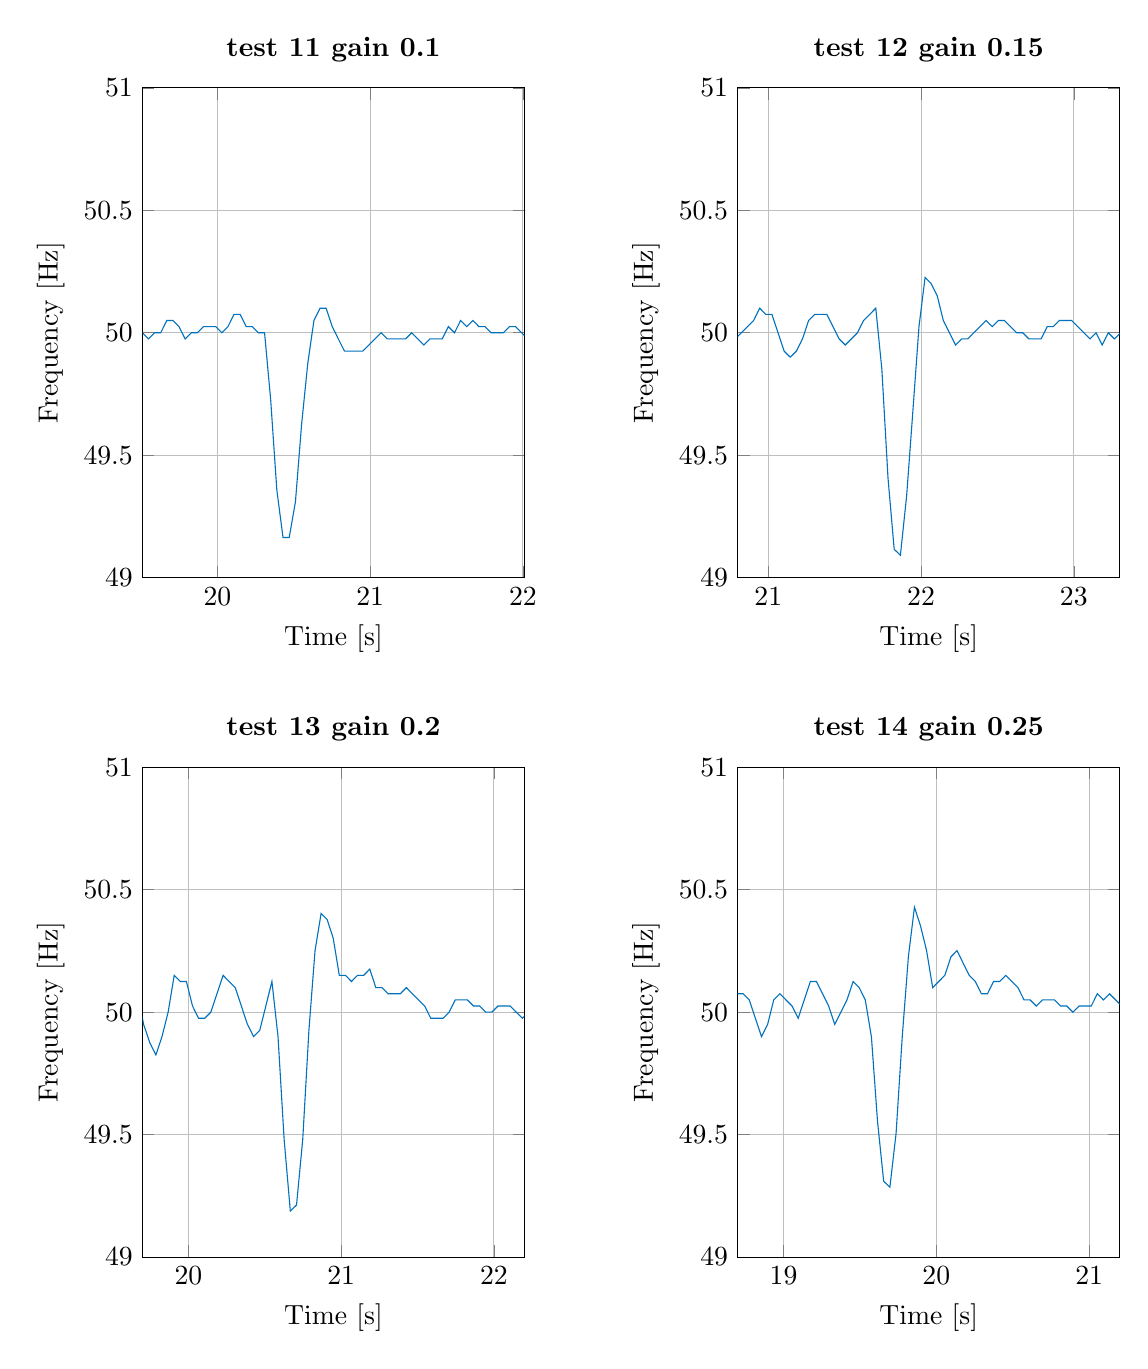
\begin{tikzpicture}

\begin{axis}[%
width=0.4\textwidth,
height=2.449in,
at={(1.024in,4.19in)},
scale only axis,
xmin=19.51,
xmax=22.01,
xlabel={Time [s]},
xmajorgrids,
ymin=49,
ymax=51,
ylabel={Frequency [Hz]},
ymajorgrids,
axis background/.style={fill=white},
title style={font=\bfseries},
title={test 11 gain 0.1}
]
\addplot [color=mycolor1,solid,forget plot]
  table[row sep=crcr]{%
19.50906	50.0000000000011\\
19.54906	49.9750124937507\\
19.58908	50.0000000000011\\
19.62908	50.0000000000011\\
19.66908	50.0500500500492\\
19.70904	50.0500500500492\\
19.749	50.0250125062532\\
19.78898	49.9750124937551\\
19.829	49.9999999999966\\
19.869	50.0000000000011\\
19.909	50.0250125062532\\
19.94898	50.0250125062532\\
19.98896	50.0250125062532\\
20.02894	50.0000000000011\\
20.06894	50.0250125062532\\
20.10892	50.0751126690017\\
20.14886	50.0751126690062\\
20.1888	50.0250125062532\\
20.22878	50.0250125062532\\
20.26876	49.9999999999966\\
20.30876	50.0000000000011\\
20.34876	49.7265042267554\\
20.38898	49.3583415597226\\
20.4295	49.1642084562416\\
20.47018	49.1642084562459\\
20.51086	49.309664694281\\
20.55142	49.627791563273\\
20.59172	49.8753117206996\\
20.63182	50.0500500500492\\
20.67178	50.1002004008033\\
20.7117	50.1002004007989\\
20.75162	50.0250125062532\\
20.7916	49.9750124937551\\
20.83162	49.9251123315022\\
20.87168	49.9251123315022\\
20.91174	49.9251123315022\\
20.9518	49.9251123315022\\
20.99186	49.9500499500529\\
21.0319	49.9750124937507\\
21.07192	50.0000000000011\\
21.11192	49.9750124937507\\
21.15194	49.9750124937551\\
21.19196	49.9750124937551\\
21.23198	49.9750124937507\\
21.272	50.0000000000011\\
21.312	49.9750124937507\\
21.35202	49.9500499500529\\
21.39206	49.9750124937507\\
21.43208	49.9750124937551\\
21.4721	49.9750124937507\\
21.51212	50.0250125062532\\
21.5521	50.0000000000011\\
21.5921	50.0500500500492\\
21.63206	50.0250125062532\\
21.67204	50.0500500500492\\
21.712	50.0250125062532\\
21.75198	50.0250125062532\\
21.79196	50.0000000000011\\
21.83196	50.0000000000011\\
21.87196	50.0000000000011\\
21.91196	50.0250125062532\\
21.95194	50.0250125062532\\
21.99192	49.9999999999966\\
22.03192	49.9750124937551\\
};
\end{axis}

\begin{axis}[%
width=0.4\textwidth,
height=2.449in,
at={(4in,4.19in)},
scale only axis,
xmin=20.8,
xmax=23.3,
xlabel={Time [s]},
xmajorgrids,
ymin=49,
ymax=51,
ylabel={Frequency [Hz]},
ymajorgrids,
axis background/.style={fill=white},
title style={font=\bfseries},
title={test 12  gain 0.15}
]
\addplot [color=mycolor1,solid,forget plot]
  table[row sep=crcr]{%
20.78386	49.9750124937507\\
20.82388	50.0000000000011\\
20.86388	50.0250125062532\\
20.90386	50.0500500500492\\
20.94382	50.1002004008033\\
20.98374	50.0751126690017\\
21.02368	50.0751126690062\\
21.06362	49.9999999999966\\
21.10362	49.9251123315022\\
21.14368	49.9001996007988\\
21.18376	49.9251123315022\\
21.22382	49.9750124937551\\
21.26384	50.0500500500492\\
21.3038	50.0751126690062\\
21.34374	50.0751126690017\\
21.38368	50.0751126690017\\
21.42362	50.0250125062532\\
21.4636	49.9750124937551\\
21.50362	49.9500499500485\\
21.54366	49.9750124937551\\
21.58368	50.0000000000011\\
21.62368	50.0500500500492\\
21.66364	50.0751126690017\\
21.70358	50.1002004008033\\
21.7435	49.8504486540358\\
21.78362	49.4071146245075\\
21.8241	49.1159135559918\\
21.86482	49.0918016691218\\
21.90556	49.3339911198816\\
21.9461	49.6770988574268\\
21.98636	50.0250125062532\\
22.02634	50.2260170768472\\
22.06616	50.2008032128493\\
22.106	50.150451354062\\
22.14588	50.0500500500492\\
22.18584	50.0000000000011\\
22.22584	49.9500499500485\\
22.26588	49.9750124937551\\
22.3059	49.9750124937507\\
22.34592	50.0000000000011\\
22.38592	50.0250125062532\\
22.4259	50.0500500500492\\
22.46586	50.0250125062532\\
22.50584	50.0500500500537\\
22.5458	50.0500500500492\\
22.58576	50.0250125062532\\
22.62574	49.9999999999966\\
22.66574	50.0000000000011\\
22.70574	49.9750124937551\\
22.74576	49.9750124937507\\
22.78578	49.9750124937551\\
22.8258	50.0250125062532\\
22.86578	50.0250125062532\\
22.90576	50.0500500500492\\
22.94572	50.0500500500492\\
22.98568	50.0500500500492\\
23.02564	50.0250125062532\\
23.06562	50.0000000000011\\
23.10562	49.9750124937551\\
23.14564	49.9999999999966\\
23.18564	49.9500499500529\\
23.22568	49.9999999999966\\
23.26568	49.9750124937551\\
23.3057	50.0000000000011\\
};
\end{axis}

\begin{axis}[%
width=0.4\textwidth,
height=2.449in,
at={(1.024in,0.793in)},
scale only axis,
xmin=19.7,
xmax=22.2,
xlabel={Time [s]},
xmajorgrids,
ymin=49,
ymax=51,
ylabel={Frequency [Hz]},
ymajorgrids,
axis background/.style={fill=white},
title style={font=\bfseries},
title={test 13  gain 0.2}
]
\addplot [color=mycolor1,solid,forget plot]
  table[row sep=crcr]{%
19.66716	50.0751126690062\\
19.7071	49.9500499500485\\
19.74714	49.8753117206996\\
19.78724	49.8256103637258\\
19.82738	49.9001996007988\\
19.86746	50.0000000000011\\
19.90746	50.150451354062\\
19.94734	50.1253132832043\\
19.98724	50.1253132832088\\
20.02714	50.0250125062532\\
20.06712	49.9750124937551\\
20.10714	49.9750124937507\\
20.14716	50.0000000000011\\
20.18716	50.0751126690062\\
20.2271	50.150451354062\\
20.26698	50.1253132832043\\
20.30688	50.1002004008033\\
20.3468	50.0250125062532\\
20.38678	49.9500499500485\\
20.42682	49.9001996007988\\
20.4669	49.9251123315022\\
20.50696	50.0250125062532\\
20.54694	50.1253132832088\\
20.58684	49.9001996007988\\
20.62692	49.4804552201868\\
20.66734	49.1883915395978\\
20.708	49.2125984251971\\
20.74864	49.4804552201868\\
20.78906	49.9251123315022\\
20.82912	50.2512562814075\\
20.86892	50.4032258064508\\
20.9086	50.3778337531488\\
20.9483	50.3018108651942\\
20.98806	50.150451354062\\
21.02794	50.150451354062\\
21.06782	50.1253132832088\\
21.10772	50.150451354062\\
21.1476	50.150451354062\\
21.18748	50.1756146512784\\
21.22734	50.1002004008033\\
21.26726	50.1002004007989\\
21.30718	50.0751126690062\\
21.34712	50.0751126690017\\
21.38706	50.0751126690017\\
21.427	50.1002004008033\\
21.46692	50.0751126690017\\
21.50686	50.0500500500537\\
21.54682	50.0250125062532\\
21.5868	49.9750124937507\\
21.62682	49.9750124937551\\
21.66684	49.9750124937507\\
21.70686	50.0000000000011\\
21.74686	50.0500500500492\\
21.78682	50.0500500500492\\
21.82678	50.0500500500537\\
21.86674	50.0250125062532\\
21.90672	50.0250125062532\\
21.9467	49.9999999999966\\
21.9867	50.0000000000011\\
22.0267	50.0250125062532\\
22.06668	50.0250125062532\\
22.10666	50.0250125062532\\
22.14664	50.0000000000011\\
22.18664	49.9750124937507\\
22.22666	50.0000000000011\\
};
\end{axis}

\begin{axis}[%
width=0.4\textwidth,
height=2.449in,
at={(4in,0.793in)},
scale only axis,
xmin=18.7,
xmax=21.2,
xlabel={Time [s]},
xmajorgrids,
ymin=49,
ymax=51,
ylabel={Frequency [Hz]},
ymajorgrids,
axis background/.style={fill=white},
title style={font=\bfseries},
title={test 14  gain 0.25}
]
\addplot [color=mycolor1,solid,forget plot]
  table[row sep=crcr]{%
18.69564	50.0751126690017\\
18.73558	50.0751126690062\\
18.77552	50.0500500500492\\
18.81548	49.9750124937507\\
18.8555	49.9001996007988\\
18.89558	49.9500499500529\\
18.93562	50.0500500500492\\
18.97558	50.0751126690017\\
19.01552	50.0500500500492\\
19.05548	50.0250125062532\\
19.09546	49.9750124937551\\
19.13548	50.0500500500492\\
19.17544	50.1253132832088\\
19.21534	50.1253132832088\\
19.25524	50.0751126690017\\
19.29518	50.0250125062532\\
19.33516	49.9500499500485\\
19.3752	50.0000000000011\\
19.4152	50.0500500500492\\
19.45516	50.1253132832088\\
19.49506	50.1002004008033\\
19.53498	50.0500500500492\\
19.57494	49.9001996007988\\
19.61502	49.5540138751242\\
19.65538	49.309664694281\\
19.69594	49.28536224741\\
19.73652	49.5049504950517\\
19.77692	49.9001996007988\\
19.817	50.2260170768428\\
19.85682	50.4286434694935\\
19.89648	50.3524672708929\\
19.9362	50.2512562814075\\
19.976	50.1002004008033\\
20.01592	50.1253132832088\\
20.05582	50.150451354062\\
20.0957	50.2260170768428\\
20.13552	50.2512562814075\\
20.17532	50.2008032128538\\
20.21516	50.150451354062\\
20.25504	50.1253132832088\\
20.29494	50.0751126690017\\
20.33488	50.0751126690017\\
20.37482	50.1253132832088\\
20.41472	50.1253132832088\\
20.45462	50.150451354062\\
20.4945	50.1253132832088\\
20.5344	50.1002004008033\\
20.57432	50.0500500500492\\
20.61428	50.0500500500492\\
20.65424	50.0250125062532\\
20.69422	50.0500500500492\\
20.73418	50.0500500500492\\
20.77414	50.0500500500492\\
20.8141	50.0250125062532\\
20.85408	50.0250125062532\\
20.89406	50.0000000000011\\
20.93406	50.0250125062532\\
20.97404	50.0250125062532\\
21.01402	50.0250125062532\\
21.054	50.0751126690017\\
21.09394	50.0500500500537\\
21.1339	50.0751126690017\\
21.17384	50.0500500500492\\
21.2138	50.0250125062532\\
};
\end{axis}
\end{tikzpicture}%
\caption{Step from 10 to 20 kW load, with various scaling factors. }
\label{fig:test11-14-10to20kwstepfreq}
\end{figure}

\begin{figure}[H]
\centering
% This file was created by matlab2tikz.
%
%The latest updates can be retrieved from
%  http://www.mathworks.com/matlabcentral/fileexchange/22022-matlab2tikz-matlab2tikz
%where you can also make suggestions and rate matlab2tikz.
%
\definecolor{mycolor1}{rgb}{0.00000,0.44700,0.74100}%
%
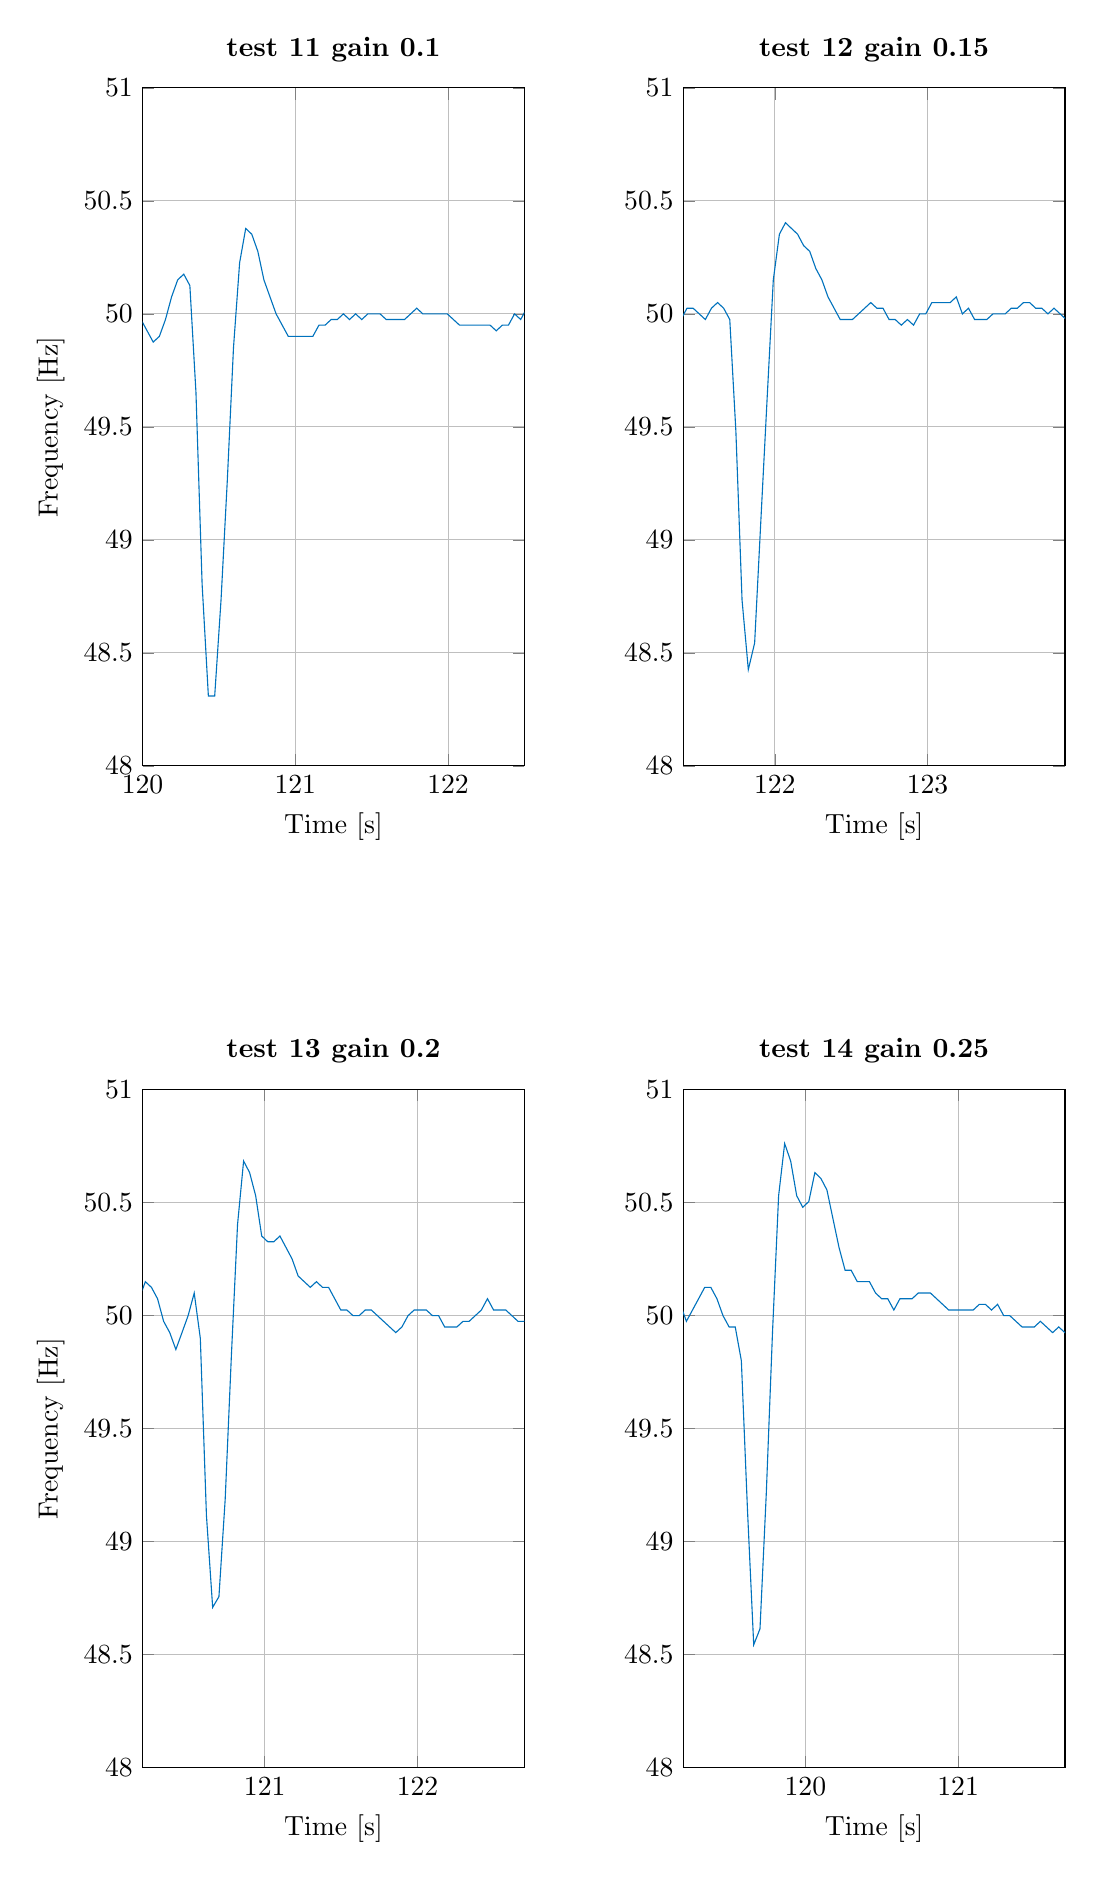
\begin{tikzpicture}

\begin{axis}[%
width=0.4\textwidth,
height=3.39in,
at={(1.297in,5.802in)},
scale only axis,
xmin=120,
xmax=122.5,
xlabel={Time [s]},
xmajorgrids,
ymin=48,
ymax=51,
ylabel={Frequency [Hz]},
ymajorgrids,
axis background/.style={fill=white},
title style={font=\bfseries},
title={test 11 gain 0.1}
]
\addplot [color=mycolor1,solid,forget plot]
  table[row sep=crcr]{%
119.98978	49.9750124937551\\
120.0298	49.9251123315066\\
120.06986	49.875311720704\\
120.10996	49.9001996007944\\
120.15004	49.9750124937551\\
120.19006	50.0751126690017\\
120.23	50.1504513540665\\
120.26988	50.1756146512739\\
120.30974	50.1253132832043\\
120.34964	49.6524329692209\\
120.38992	48.8042947779349\\
120.4309	48.3091787439662\\
120.4723	48.3091787439662\\
120.5137	48.7329434697743\\
120.55474	49.2610837438451\\
120.59534	49.8504486540358\\
120.63546	50.2260170768562\\
120.67528	50.3778337531353\\
120.71498	50.3524672708929\\
120.7547	50.2765208647647\\
120.79448	50.1504513540665\\
120.83436	50.0751126690017\\
120.8743	49.9999999999922\\
120.9143	49.9500499500618\\
120.95434	49.9001996007944\\
120.99442	49.9001996007944\\
121.0345	49.9001996007944\\
121.07458	49.9001996008121\\
121.11466	49.9001996007944\\
121.15474	49.950049950044\\
121.19478	49.950049950044\\
121.23482	49.9750124937551\\
121.27484	49.9750124937551\\
121.31486	50.0000000000099\\
121.35486	49.9750124937551\\
121.39488	49.9999999999922\\
121.43488	49.9750124937551\\
121.4749	49.9999999999922\\
121.5149	50.0000000000099\\
121.5549	49.9999999999922\\
121.5949	49.9750124937551\\
121.63492	49.9750124937551\\
121.67494	49.9750124937551\\
121.71496	49.9750124937551\\
121.75498	49.9999999999922\\
121.79498	50.0250125062532\\
121.83496	50.0000000000099\\
121.87496	49.9999999999922\\
121.91496	50.0000000000099\\
121.95496	49.9999999999922\\
121.99496	49.9999999999922\\
122.03496	49.9750124937551\\
122.07498	49.9500499500618\\
122.11502	49.950049950044\\
122.15506	49.950049950044\\
122.1951	49.9500499500618\\
122.23514	49.950049950044\\
122.27518	49.950049950044\\
122.31522	49.9251123315066\\
122.35528	49.950049950044\\
122.39532	49.9500499500618\\
122.43536	49.9999999999922\\
122.47536	49.9750124937551\\
122.51538	50.0250125062532\\
};
\end{axis}

\begin{axis}[%
width=0.4\textwidth,
height=3.39in,
at={(4in,5.802in)},
scale only axis,
xmin=121.4,
xmax=123.9,
xlabel={Time [s]},
xmajorgrids,
ymin=48,
ymax=51,
ymajorgrids,
axis background/.style={fill=white},
title style={font=\bfseries},
title={test 12  gain 0.15}
]
\addplot [color=mycolor1,solid,forget plot]
  table[row sep=crcr]{%
121.38532	49.9750124937551\\
121.42534	50.0250125062532\\
121.46532	50.0250125062532\\
121.5053	49.9999999999922\\
121.5453	49.9750124937551\\
121.58532	50.0250125062532\\
121.6253	50.0500500500581\\
121.66526	50.0250125062532\\
121.70524	49.9750124937551\\
121.74526	49.4804552201737\\
121.78568	48.7329434697912\\
121.82672	48.4261501210741\\
121.86802	48.5436893203843\\
121.90922	49.0918016691218\\
121.94996	49.627791563273\\
121.99026	50.1504513540665\\
122.03014	50.3524672708929\\
122.06986	50.4032258064463\\
122.10954	50.3778337531533\\
122.14924	50.3524672708929\\
122.18896	50.3018108651897\\
122.22872	50.2765208647647\\
122.2685	50.2008032128538\\
122.30834	50.1504513540486\\
122.34822	50.0751126690017\\
122.38816	50.0250125062532\\
122.42814	49.9750124937551\\
122.46816	49.9750124937551\\
122.50818	49.9750124937551\\
122.5482	50.0000000000099\\
122.5882	50.0250125062532\\
122.62818	50.0500500500403\\
122.66814	50.0250125062532\\
122.70812	50.0250125062532\\
122.7481	49.9750124937551\\
122.78812	49.9750124937551\\
122.82814	49.950049950044\\
122.86818	49.9750124937551\\
122.9082	49.950049950044\\
122.94824	50.0000000000099\\
122.98824	49.9999999999922\\
123.02824	50.0500500500581\\
123.0682	50.0500500500403\\
123.10816	50.0500500500581\\
123.14812	50.0500500500403\\
123.18808	50.0751126690195\\
123.22802	49.9999999999922\\
123.26802	50.0250125062532\\
123.308	49.9750124937551\\
123.34802	49.9750124937551\\
123.38804	49.9750124937551\\
123.42806	49.9999999999922\\
123.46806	50.0000000000099\\
123.50806	49.9999999999922\\
123.54806	50.0250125062532\\
123.58804	50.0250125062532\\
123.62802	50.0500500500581\\
123.66798	50.0500500500403\\
123.70794	50.0250125062532\\
123.74792	50.0250125062532\\
123.7879	50.0000000000099\\
123.8279	50.0250125062355\\
123.86788	50.0000000000099\\
123.90788	49.9750124937551\\
};
\end{axis}

\begin{axis}[%
width=0.4\textwidth,
height=3.39in,
at={(1.297in,0.793in)},
scale only axis,
xmin=120.2,
xmax=122.7,
xlabel={Time [s]},
xmajorgrids,
ymin=48,
ymax=51,
ylabel={Frequency [Hz]},
ymajorgrids,
axis background/.style={fill=white},
title style={font=\bfseries},
title={test 13  gain 0.2}
]
\addplot [color=mycolor1,solid,forget plot]
  table[row sep=crcr]{%
120.17836	50.0751126690017\\
120.2183	50.1504513540665\\
120.25818	50.1253132832043\\
120.29808	50.0751126690195\\
120.33802	49.9750124937374\\
120.37804	49.9251123315066\\
120.4181	49.8504486540358\\
120.45822	49.9251123315066\\
120.49828	50.0000000000099\\
120.53828	50.10020040079\\
120.5782	49.9001996007944\\
120.61828	49.1159135560003\\
120.659	48.7092060399396\\
120.70006	48.7567040468027\\
120.74108	49.1883915395935\\
120.78174	49.8256103637346\\
120.82188	50.4032258064463\\
120.86156	50.6842372022414\\
120.90102	50.6329113924001\\
120.94052	50.5305709954512\\
120.9801	50.3524672708929\\
121.01982	50.3271263210937\\
121.05956	50.3271263210757\\
121.0993	50.3524672709109\\
121.13902	50.3018108651897\\
121.17878	50.2512562814075\\
121.21858	50.1756146512739\\
121.25844	50.1504513540665\\
121.29832	50.1253132832043\\
121.33822	50.1504513540665\\
121.3781	50.1253132832043\\
121.418	50.1253132832043\\
121.4579	50.0751126690017\\
121.49784	50.0250125062532\\
121.53782	50.0250125062532\\
121.5778	50.0000000000099\\
121.6178	49.9999999999922\\
121.6578	50.0250125062532\\
121.69778	50.0250125062532\\
121.73776	50.0000000000099\\
121.77776	49.9750124937374\\
121.81778	49.9500499500618\\
121.85782	49.9251123315066\\
121.89788	49.950049950044\\
121.93792	49.9999999999922\\
121.97792	50.0250125062532\\
122.0179	50.0250125062532\\
122.05788	50.0250125062532\\
122.09786	50.0000000000099\\
122.13786	49.9999999999922\\
122.17786	49.9500499500618\\
122.2179	49.950049950044\\
122.25794	49.950049950044\\
122.29798	49.9750124937551\\
122.338	49.9750124937551\\
122.37802	49.9999999999922\\
122.41802	50.0250125062532\\
122.458	50.0751126690195\\
122.49794	50.0250125062532\\
122.53792	50.0250125062355\\
122.5779	50.0250125062532\\
122.61788	50.0000000000099\\
122.65788	49.9750124937551\\
122.6979	49.9750124937551\\
122.73792	49.9999999999922\\
};
\end{axis}

\begin{axis}[%
width=0.4\textwidth,
height=3.39in,
at={(4in,0.793in)},
scale only axis,
xmin=119.2,
xmax=121.7,
xlabel={Time [s]},
xmajorgrids,
ymin=48,
ymax=51,
ymajorgrids,
axis background/.style={fill=white},
title style={font=\bfseries},
title={test 14  gain 0.25}
]
\addplot [color=mycolor1,solid,forget plot]
  table[row sep=crcr]{%
119.18136	50.0500500500581\\
119.22132	49.9750124937551\\
119.26134	50.0250125062532\\
119.30132	50.0751126690017\\
119.34126	50.1253132832043\\
119.38116	50.1253132832043\\
119.42106	50.0751126690017\\
119.461	50.0000000000099\\
119.501	49.950049950044\\
119.54104	49.9500499500618\\
119.58108	49.8007968127488\\
119.62124	49.1400491400479\\
119.66194	48.5436893203843\\
119.70314	48.6144871171625\\
119.74428	49.2125984251842\\
119.78492	49.9251123315066\\
119.82498	50.5305709954512\\
119.86456	50.7614213197962\\
119.90396	50.6842372022414\\
119.94342	50.5305709954512\\
119.983	50.47955577991\\
120.02262	50.5050505050413\\
120.06222	50.6329113924183\\
120.10172	50.6072874493796\\
120.14124	50.5561172901992\\
120.1808	50.4286434694935\\
120.22046	50.3018108651897\\
120.26022	50.2008032128538\\
120.30006	50.2008032128538\\
120.3399	50.1504513540486\\
120.37978	50.1504513540665\\
120.41966	50.1504513540665\\
120.45954	50.10020040079\\
120.49946	50.0751126690195\\
120.5394	50.0751126690017\\
120.57934	50.0250125062532\\
120.61932	50.0751126690017\\
120.65926	50.0751126690017\\
120.6992	50.0751126690017\\
120.73914	50.1002004008078\\
120.77906	50.10020040079\\
120.81898	50.1002004008078\\
120.8589	50.0751126690017\\
120.89884	50.0500500500581\\
120.9388	50.0250125062532\\
120.97878	50.0250125062532\\
121.01876	50.0250125062532\\
121.05874	50.0250125062532\\
121.09872	50.0250125062532\\
121.1387	50.0500500500403\\
121.17866	50.0500500500581\\
121.21862	50.0250125062532\\
121.2586	50.0500500500403\\
121.29856	50.0000000000099\\
121.33856	49.9999999999922\\
121.37856	49.9750124937551\\
121.41858	49.950049950044\\
121.45862	49.9500499500618\\
121.49866	49.950049950044\\
121.5387	49.9750124937551\\
121.57872	49.950049950044\\
121.61876	49.9251123315066\\
121.65882	49.950049950044\\
121.69886	49.9251123315066\\
121.73892	49.950049950044\\
};
\end{axis}
\end{tikzpicture}%
\caption{Step from 10 to 30 kW load, with various scaling factors.}
\label{fig:test11-14-10to30kwstepfreq}
\end{figure}

\begin{figure}[H]
\centering
% This file was created by matlab2tikz.
%
%The latest updates can be retrieved from
%  http://www.mathworks.com/matlabcentral/fileexchange/22022-matlab2tikz-matlab2tikz
%where you can also make suggestions and rate matlab2tikz.
%
\definecolor{mycolor1}{rgb}{0.00000,0.44700,0.74100}%
%
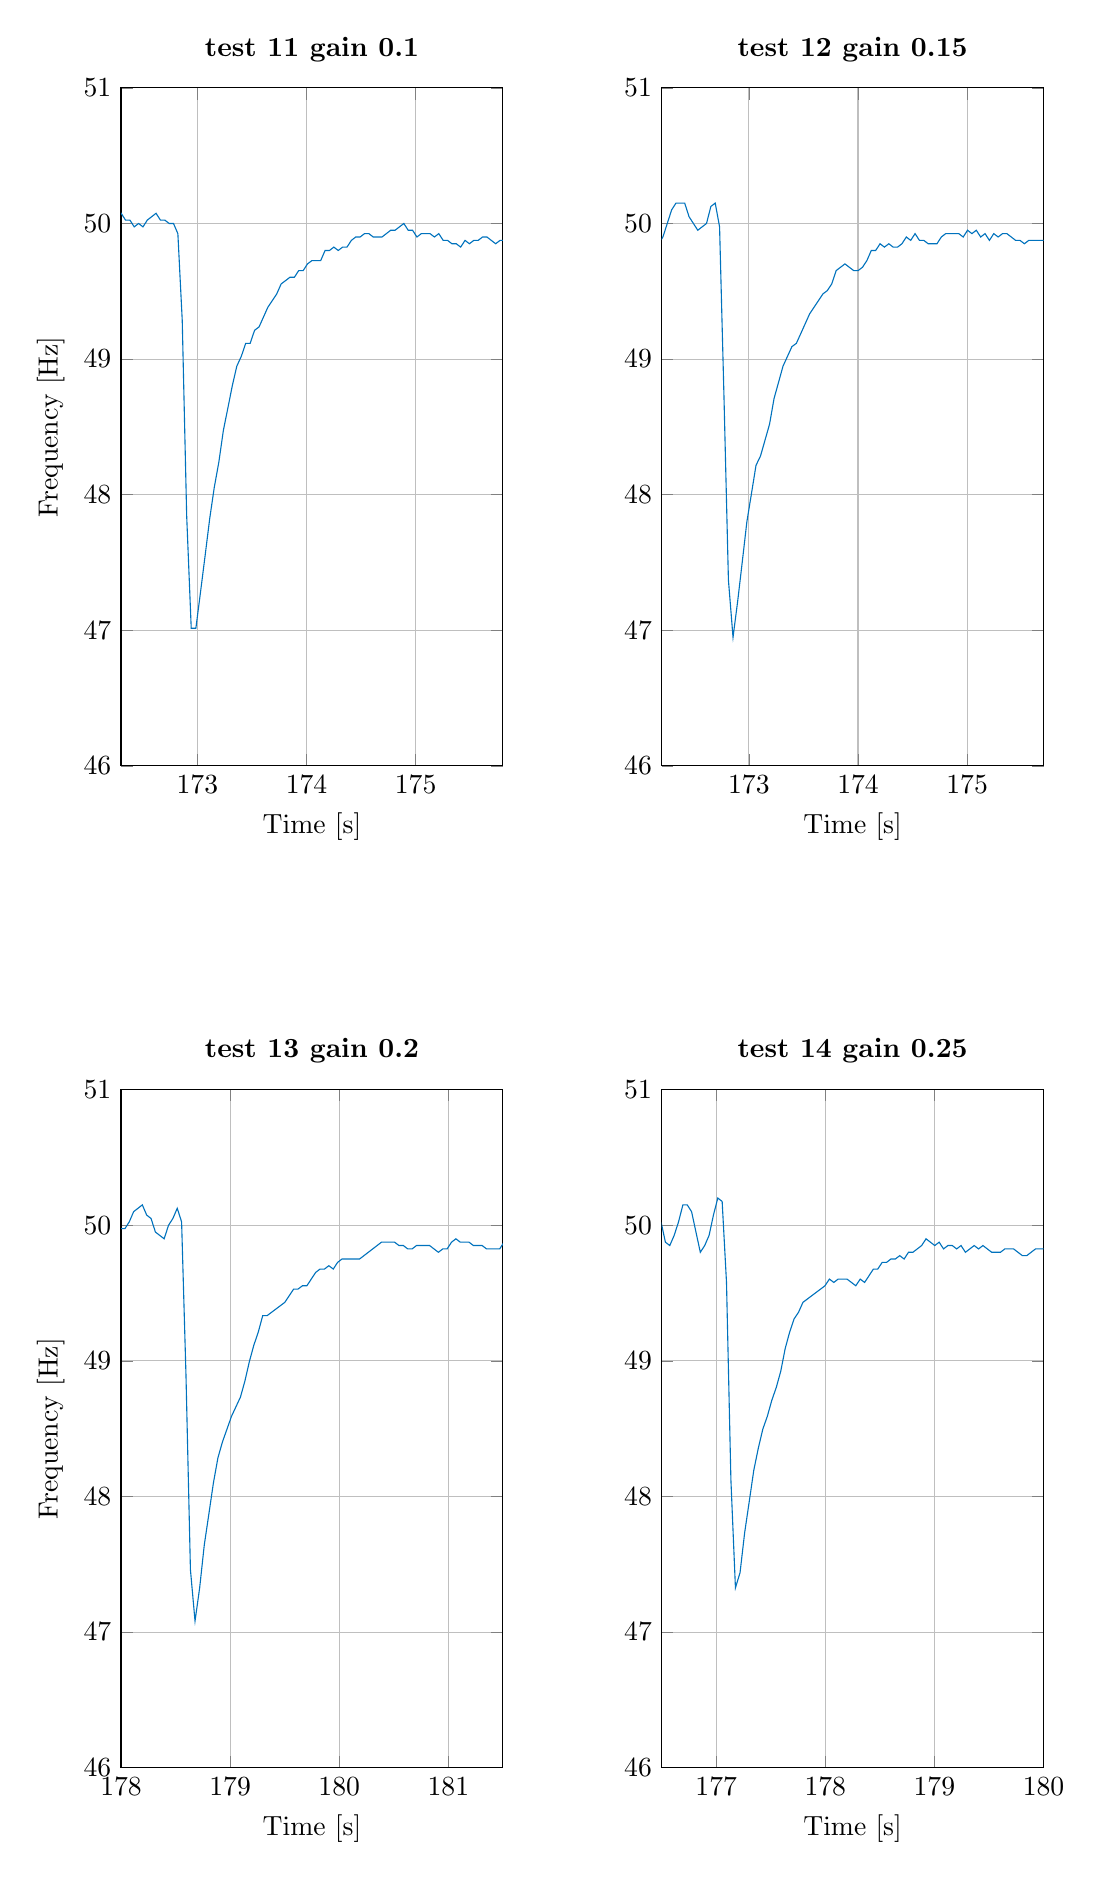
\begin{tikzpicture}

\begin{axis}[%
width=0.4\textwidth,
height=3.39in,
at={(1.297in,5.802in)},
scale only axis,
xmin=172.3,
xmax=175.8,
xlabel={Time [s]},
xmajorgrids,
ymin=46,
ymax=51,
ylabel={Frequency [Hz]},
ymajorgrids,
axis background/.style={fill=white},
title style={font=\bfseries},
title={test 11 gain 0.1}
]
\addplot [color=mycolor1,solid,forget plot]
  table[row sep=crcr]{%
172.26122	50.025012506271\\
172.3012	50.0751126690017\\
172.34114	50.0250125062355\\
172.38112	50.025012506271\\
172.4211	49.9750124937551\\
172.46112	49.9999999999744\\
172.50112	49.9750124937551\\
172.54114	50.025012506271\\
172.58112	50.0500500500403\\
172.62108	50.0751126690017\\
172.66102	50.025012506271\\
172.701	50.0250125062355\\
172.74098	50.0000000000099\\
172.78098	50.0000000000099\\
172.82098	49.9251123314889\\
172.86104	49.2853622474057\\
172.90162	47.8468899521589\\
172.94342	47.0145745180979\\
172.98596	47.0145745180979\\
173.0285	47.2813238770874\\
173.0708	47.5511174512368\\
173.11286	47.8240076518397\\
173.15468	48.0538202787183\\
173.1963	48.2392667631444\\
173.23776	48.4730974309328\\
173.27902	48.6381322957122\\
173.32014	48.8042947779518\\
173.36112	48.947626040126\\
173.40198	49.0196078431491\\
173.44278	49.1159135560003\\
173.4835	49.1159135559661\\
173.52422	49.2125984252014\\
173.56486	49.2368291482151\\
173.60548	49.309664694281\\
173.64604	49.3827160493722\\
173.68654	49.4315373208156\\
173.727	49.4804552202085\\
173.76742	49.554013875098\\
173.80778	49.5785820525702\\
173.84812	49.6031746031643\\
173.88844	49.6031746031643\\
173.92876	49.6524329692209\\
173.96904	49.6524329692209\\
174.00932	49.7017892643995\\
174.04956	49.7265042267818\\
174.08978	49.7265042267466\\
174.13	49.7265042267466\\
174.17022	49.8007968127311\\
174.21038	49.8007968127664\\
174.25054	49.825610363717\\
174.29068	49.8007968127664\\
174.33084	49.825610363717\\
174.37098	49.825610363717\\
174.41112	49.875311720704\\
174.45122	49.9001996008121\\
174.4913	49.9001996007767\\
174.53138	49.9251123315244\\
174.57144	49.9251123314889\\
174.6115	49.9001996008121\\
174.65158	49.9001996007767\\
174.69166	49.9001996008121\\
174.73174	49.9251123314889\\
174.7718	49.9500499500795\\
174.81184	49.950049950044\\
174.85188	49.9750124937551\\
174.8919	49.9999999999744\\
174.9319	49.9500499500795\\
174.97194	49.950049950044\\
175.01198	49.9001996007767\\
175.05206	49.9251123315244\\
175.09212	49.9251123314889\\
175.13218	49.9251123314889\\
175.17224	49.9001996008121\\
175.21232	49.9251123315244\\
175.25238	49.8753117206687\\
175.29248	49.875311720704\\
175.33258	49.8504486540358\\
175.3727	49.8504486540358\\
175.41282	49.8256103637522\\
175.45296	49.8753117206687\\
175.49306	49.8504486540711\\
175.53318	49.8753117206687\\
175.57328	49.875311720704\\
175.61338	49.9001996008121\\
175.65346	49.9001996007767\\
175.69354	49.875311720704\\
175.73364	49.8504486540358\\
175.77376	49.875311720704\\
175.81386	49.875311720704\\
};
\end{axis}

\begin{axis}[%
width=0.4\textwidth,
height=3.39in,
at={(4in,5.802in)},
scale only axis,
xmin=172.2,
xmax=175.7,
xlabel={Time [s]},
xmajorgrids,
ymin=46,
ymax=51,
ymajorgrids,
axis background/.style={fill=white},
title style={font=\bfseries},
title={test 12  gain 0.15}
]
\addplot [color=mycolor1,solid,forget plot]
  table[row sep=crcr]{%
172.17156	49.8504486540358\\
172.21168	49.9001996008121\\
172.25176	49.9999999999744\\
172.29176	50.1002004008078\\
172.33168	50.1504513540486\\
172.37156	50.1504513540844\\
172.41144	50.1504513540486\\
172.45132	50.0500500500759\\
172.49128	49.9999999999744\\
172.53128	49.950049950044\\
172.57132	49.9750124937551\\
172.61134	50.0000000000099\\
172.65134	50.1253132832222\\
172.69124	50.1504513540486\\
172.73112	49.9750124937551\\
172.77114	48.7329434697743\\
172.81218	47.3709142586607\\
172.8544	46.9483568075194\\
172.897	47.2143531633592\\
172.93936	47.5059382422747\\
172.98146	47.8011472275247\\
173.0233	48.0076812289882\\
173.06496	48.2160077145861\\
173.10644	48.285852245273\\
173.14786	48.4027105518088\\
173.18918	48.5201358563689\\
173.2304	48.7092060399564\\
173.27146	48.8281249999851\\
173.31242	48.947626040126\\
173.35328	49.0196078431491\\
173.39408	49.0918016691218\\
173.43482	49.1159135560003\\
173.47554	49.1883915395935\\
173.5162	49.2610837438279\\
173.5568	49.3339911198902\\
173.59734	49.3827160493722\\
173.63784	49.4315373208156\\
173.6783	49.4804552202085\\
173.71872	49.504950495043\\
173.75912	49.5540138751329\\
173.79948	49.6524329691858\\
173.83976	49.6770988574399\\
173.88002	49.7017892643995\\
173.92026	49.6770988574399\\
173.96052	49.6524329692209\\
174.0008	49.6524329692209\\
174.04108	49.6770988574049\\
174.08134	49.7265042267466\\
174.12156	49.8007968127664\\
174.16172	49.8007968127664\\
174.20188	49.8504486540358\\
174.242	49.825610363717\\
174.28214	49.8504486540358\\
174.32226	49.825610363717\\
174.3624	49.825610363717\\
174.40254	49.8504486540358\\
174.44266	49.9001996008121\\
174.48274	49.875311720704\\
174.52284	49.9251123314889\\
174.5629	49.875311720704\\
174.603	49.875311720704\\
174.6431	49.8504486540358\\
174.68322	49.8504486540358\\
174.72334	49.8504486540358\\
174.76346	49.9001996008121\\
174.80354	49.9251123314889\\
174.8436	49.9251123315244\\
174.88366	49.9251123314889\\
174.92372	49.9251123314889\\
174.96378	49.9001996008121\\
175.00386	49.950049950044\\
175.0439	49.9251123315244\\
175.08396	49.950049950044\\
175.124	49.9001996007767\\
175.16408	49.9251123315244\\
175.20414	49.875311720704\\
175.24424	49.9251123314889\\
175.2843	49.9001996008121\\
175.32438	49.9251123314889\\
175.36444	49.9251123314889\\
175.4045	49.9001996008121\\
175.44458	49.875311720704\\
175.48468	49.875311720704\\
175.52478	49.8504486540358\\
175.5649	49.875311720704\\
175.605	49.8753117206687\\
175.6451	49.875311720704\\
175.6852	49.875311720704\\
175.7253	49.875311720704\\
};
\end{axis}

\begin{axis}[%
width=0.4\textwidth,
height=3.39in,
at={(1.297in,0.793in)},
scale only axis,
xmin=178,
xmax=181.5,
xlabel={Time [s]},
xmajorgrids,
ymin=46,
ymax=51,
ylabel={Frequency [Hz]},
ymajorgrids,
axis background/.style={fill=white},
title style={font=\bfseries},
title={test 13  gain 0.2}
]
\addplot [color=mycolor1,solid,forget plot]
  table[row sep=crcr]{%
177.99554	49.9750124937551\\
178.03556	49.9750124937551\\
178.07558	50.025012506271\\
178.11556	50.1002004007721\\
178.15548	50.1253132832222\\
178.19538	50.1504513540486\\
178.23526	50.0751126690017\\
178.2752	50.0500500500759\\
178.31516	49.950049950044\\
178.3552	49.9251123314889\\
178.39526	49.9001996008121\\
178.43534	50.0000000000099\\
178.47534	50.0500500500403\\
178.5153	50.1253132831865\\
178.5552	50.025012506271\\
178.59518	48.8997555012303\\
178.63608	47.4608448030177\\
178.67822	47.0809792843875\\
178.7207	47.3260766682455\\
178.76296	47.6417341590965\\
178.80494	47.8697941598982\\
178.84672	48.100048100069\\
178.8883	48.285852245273\\
178.92972	48.4027105518088\\
178.97104	48.4966052376144\\
179.01228	48.5908649174064\\
179.05344	48.6618004866178\\
179.09454	48.7329434697743\\
179.13558	48.8519785051221\\
179.17652	48.9955903968685\\
179.21734	49.1159135560003\\
179.25806	49.2125984252014\\
179.2987	49.3339911198902\\
179.33924	49.3339911198556\\
179.37978	49.35834155974\\
179.4203	49.3827160493722\\
179.4608	49.4071146245031\\
179.50128	49.4315373208156\\
179.54174	49.4804552201737\\
179.58216	49.5294700347068\\
179.62254	49.529470034637\\
179.66292	49.5540138751329\\
179.70328	49.5540138751329\\
179.74364	49.6031746031643\\
179.78396	49.6524329692209\\
179.82424	49.6770988574399\\
179.8645	49.6770988574049\\
179.90476	49.7017892644346\\
179.945	49.6770988574049\\
179.98526	49.7265042267818\\
180.02548	49.751243781061\\
180.06568	49.7512437810962\\
180.10588	49.7512437810962\\
180.14608	49.7512437810962\\
180.18628	49.7512437810962\\
180.22648	49.7760079641708\\
180.26666	49.8007968127664\\
180.30682	49.825610363717\\
180.34696	49.8504486540358\\
180.38708	49.875311720704\\
180.42718	49.875311720704\\
180.46728	49.8753117206687\\
180.50738	49.875311720704\\
180.54748	49.8504486540358\\
180.5876	49.8504486540358\\
180.62772	49.8256103637522\\
180.66786	49.825610363717\\
180.708	49.8504486540358\\
180.74812	49.8504486540358\\
180.78824	49.8504486540358\\
180.82836	49.8504486540358\\
180.86848	49.825610363717\\
180.90862	49.8007968127664\\
180.94878	49.825610363717\\
180.98892	49.8256103637522\\
181.02906	49.8753117206687\\
181.06916	49.9001996008121\\
181.10924	49.875311720704\\
181.14934	49.875311720704\\
181.18944	49.8753117206687\\
181.22954	49.8504486540358\\
181.26966	49.8504486540711\\
181.30978	49.8504486540358\\
181.3499	49.825610363717\\
181.39004	49.825610363717\\
181.43018	49.8256103637522\\
181.47032	49.825610363717\\
181.51046	49.875311720704\\
};
\end{axis}

\begin{axis}[%
width=0.4\textwidth,
height=3.39in,
at={(4in,0.793in)},
scale only axis,
xmin=176.5,
xmax=180,
xlabel={Time [s]},
xmajorgrids,
ymin=46,
ymax=51,
ymajorgrids,
axis background/.style={fill=white},
title style={font=\bfseries},
title={test 14  gain 0.25}
]
\addplot [color=mycolor1,solid,forget plot]
  table[row sep=crcr]{%
176.49468	50.0250125062355\\
176.53466	49.875311720704\\
176.57476	49.8504486540358\\
176.61488	49.9251123314889\\
176.65494	50.025012506271\\
176.69492	50.1504513540486\\
176.7348	50.1504513540486\\
176.77468	50.1002004008078\\
176.8146	49.9500499500795\\
176.85464	49.8007968127311\\
176.8948	49.8504486540358\\
176.93492	49.9251123315244\\
176.97498	50.0751126690017\\
177.01492	50.200803212818\\
177.05476	50.1756146513097\\
177.09462	49.5785820525352\\
177.13496	48.1231953801686\\
177.17652	47.3260766682455\\
177.21878	47.438330170783\\
177.26094	47.7326968973767\\
177.30284	47.9616306954533\\
177.34454	48.1927710843218\\
177.38604	48.3558994197322\\
177.4274	48.4966052376478\\
177.46864	48.5908649173729\\
177.5098	48.7092060399564\\
177.55086	48.8042947779518\\
177.59184	48.9236790606467\\
177.63272	49.0918016691218\\
177.67346	49.2125984252014\\
177.7141	49.309664694281\\
177.75466	49.35834155974\\
177.79518	49.4315373207809\\
177.83564	49.4559841740978\\
177.87608	49.4804552201737\\
177.9165	49.5049504950778\\
177.9569	49.529470034637\\
177.99728	49.5540138751329\\
178.03764	49.6031746031993\\
178.07796	49.5785820525352\\
178.1183	49.6031746031643\\
178.15862	49.6031746031993\\
178.19894	49.6031746031643\\
178.23926	49.5785820525702\\
178.2796	49.554013875098\\
178.31996	49.6031746031643\\
178.36028	49.5785820525702\\
178.40062	49.627791563273\\
178.44092	49.6770988574399\\
178.48118	49.6770988574049\\
178.52144	49.7265042267818\\
178.56166	49.7265042267466\\
178.60188	49.7512437810962\\
178.64208	49.7512437810962\\
178.68228	49.7760079641356\\
178.72246	49.7512437810962\\
178.76266	49.8007968127664\\
178.80282	49.8007968127311\\
178.84298	49.8256103637522\\
178.88312	49.8504486540358\\
178.92324	49.9001996007767\\
178.96332	49.875311720704\\
179.00342	49.8504486540358\\
179.04354	49.875311720704\\
179.08364	49.825610363717\\
179.12378	49.8504486540358\\
179.1639	49.8504486540358\\
179.20402	49.8256103637522\\
179.24416	49.8504486540358\\
179.28428	49.8007968127311\\
179.32444	49.8256103637522\\
179.36458	49.8504486540358\\
179.4047	49.825610363717\\
179.44484	49.8504486540358\\
179.48496	49.825610363717\\
179.5251	49.8007968127664\\
179.56526	49.8007968127311\\
179.60542	49.8007968127664\\
179.64558	49.825610363717\\
179.68572	49.825610363717\\
179.72586	49.8256103637522\\
179.766	49.8007968127311\\
179.80616	49.7760079641708\\
179.84634	49.7760079641708\\
179.88652	49.8007968127311\\
179.92668	49.825610363717\\
179.96682	49.8256103637522\\
180.00696	49.825610363717\\
};
\end{axis}
\end{tikzpicture}%
\caption{Step from 10 to 50 kW load, with various scaling factors.}
\label{fig:test11-14-10to50kwstepfreq}
\end{figure}

\begin{figure}[H]
\centering
% This file was created by matlab2tikz.
%
%The latest updates can be retrieved from
%  http://www.mathworks.com/matlabcentral/fileexchange/22022-matlab2tikz-matlab2tikz
%where you can also make suggestions and rate matlab2tikz.
%
\definecolor{mycolor1}{rgb}{0.00000,0.44700,0.74100}%
%
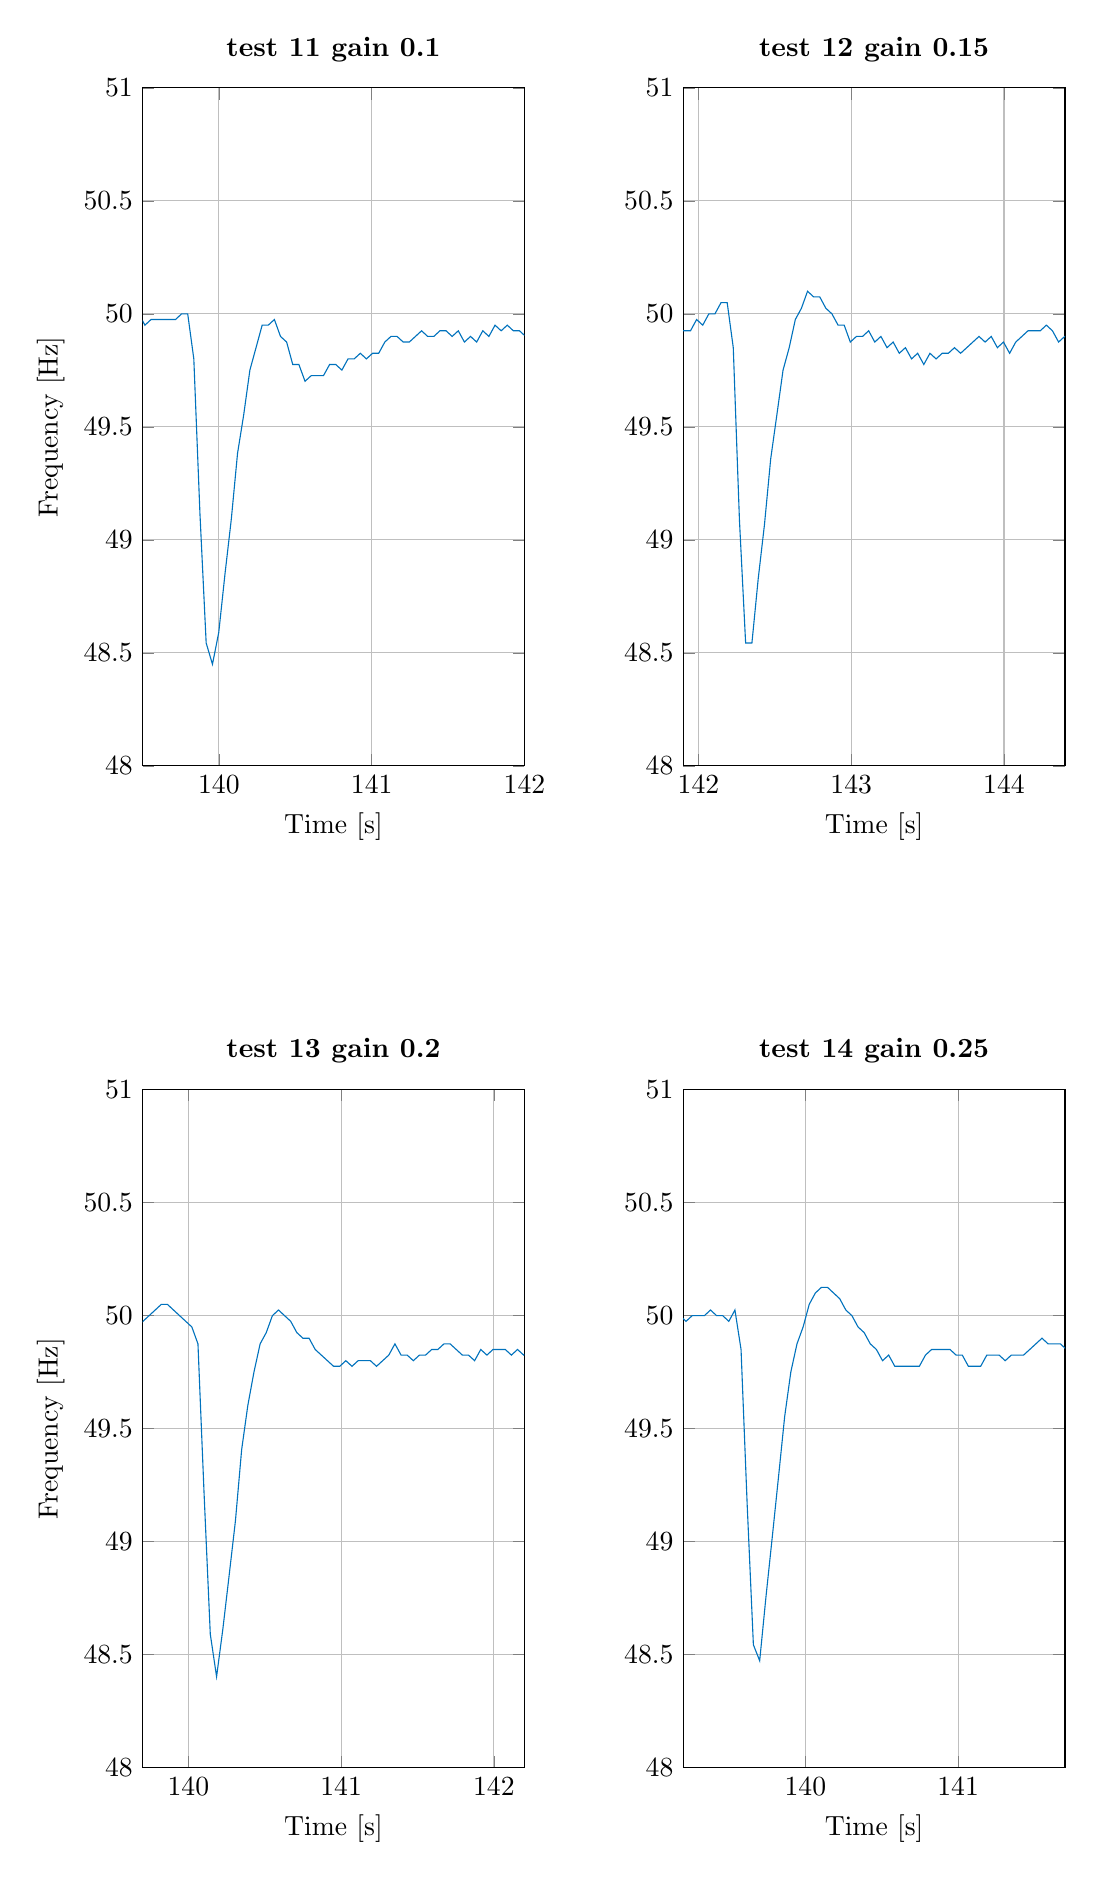
\begin{tikzpicture}

\begin{axis}[%
width=0.4\textwidth,
height=3.39in,
at={(1.297in,5.802in)},
scale only axis,
xmin=139.5,
xmax=142,
xlabel={Time [s]},
xmajorgrids,
ymin=48,
ymax=51,
ylabel={Frequency [Hz]},
ymajorgrids,
axis background/.style={fill=white},
title style={font=\bfseries},
title={test 11 gain 0.1}
]
\addplot [color=mycolor1,solid,forget plot]
  table[row sep=crcr]{%
139.47548	50.0000000000099\\
139.51548	49.950049950044\\
139.55552	49.9750124937551\\
139.59554	49.9750124937551\\
139.63556	49.9750124937551\\
139.67558	49.9750124937551\\
139.7156	49.9750124937551\\
139.75562	49.9999999999744\\
139.79562	50.0000000000099\\
139.83562	49.8007968127664\\
139.87578	49.1159135559661\\
139.9165	48.5436893203843\\
139.9577	48.4496124031336\\
139.99898	48.5908649173729\\
140.04014	48.8519785051221\\
140.08108	49.0918016691218\\
140.12182	49.3827160494068\\
140.16232	49.554013875098\\
140.20268	49.7512437810962\\
140.24288	49.8504486540358\\
140.283	49.950049950044\\
140.32304	49.9500499500795\\
140.36308	49.9750124937551\\
140.4031	49.9001996007767\\
140.44318	49.875311720704\\
140.48328	49.7760079641708\\
140.52346	49.7760079641708\\
140.56364	49.7017892643995\\
140.60388	49.7265042267466\\
140.6441	49.7265042267466\\
140.68432	49.7265042267466\\
140.72454	49.7760079641708\\
140.76472	49.7760079641708\\
140.8049	49.7512437810962\\
140.8451	49.8007968127664\\
140.88526	49.8007968127311\\
140.92542	49.825610363717\\
140.96556	49.8007968127664\\
141.00572	49.825610363717\\
141.04586	49.825610363717\\
141.086	49.875311720704\\
141.1261	49.9001996008121\\
141.16618	49.9001996007767\\
141.20626	49.875311720704\\
141.24636	49.875311720704\\
141.28646	49.9001996008121\\
141.32654	49.9251123314889\\
141.3666	49.9001996007767\\
141.40668	49.9001996008121\\
141.44676	49.9251123315244\\
141.48682	49.9251123314889\\
141.52688	49.9001996008121\\
141.56696	49.9251123314889\\
141.60702	49.875311720704\\
141.64712	49.9001996008121\\
141.6872	49.8753117206687\\
141.7273	49.9251123315244\\
141.76736	49.9001996007767\\
141.80744	49.9500499500795\\
141.84748	49.9251123314889\\
141.88754	49.950049950044\\
141.92758	49.9251123315244\\
141.96764	49.9251123314889\\
142.0077	49.9001996007767\\
};
\end{axis}

\begin{axis}[%
width=0.4\textwidth,
height=3.39in,
at={(4in,5.802in)},
scale only axis,
xmin=141.9,
xmax=144.4,
xlabel={Time [s]},
xmajorgrids,
ymin=48,
ymax=51,
ymajorgrids,
axis background/.style={fill=white},
title style={font=\bfseries},
title={test 12  gain 0.15}
]
\addplot [color=mycolor1,solid,forget plot]
  table[row sep=crcr]{%
141.86802	49.9251123314889\\
141.90808	49.9251123315244\\
141.94814	49.9251123314889\\
141.9882	49.9750124937551\\
142.02822	49.950049950044\\
142.06826	50.0000000000099\\
142.10826	49.9999999999744\\
142.14826	50.0500500500759\\
142.18822	50.0500500500403\\
142.22818	49.8504486540358\\
142.2683	49.0918016691218\\
142.30904	48.5436893203843\\
142.35024	48.5436893203843\\
142.39144	48.8281250000189\\
142.4324	49.0677134445464\\
142.47316	49.35834155974\\
142.51368	49.554013875098\\
142.55404	49.7512437810962\\
142.59424	49.8504486540358\\
142.63436	49.9750124937551\\
142.67438	50.025012506271\\
142.71436	50.1002004007721\\
142.75428	50.0751126690374\\
142.79422	50.0751126690017\\
142.83416	50.0250125062355\\
142.87414	50.0000000000099\\
142.91414	49.950049950044\\
142.95418	49.950049950044\\
142.99422	49.875311720704\\
143.03432	49.9001996008121\\
143.0744	49.9001996007767\\
143.11448	49.9251123315244\\
143.15454	49.8753117206687\\
143.19464	49.9001996008121\\
143.23472	49.8504486540358\\
143.27484	49.875311720704\\
143.31494	49.825610363717\\
143.35508	49.8504486540358\\
143.3952	49.8007968127664\\
143.43536	49.825610363717\\
143.4755	49.7760079641708\\
143.51568	49.825610363717\\
143.55582	49.8007968127664\\
143.59598	49.825610363717\\
143.63612	49.825610363717\\
143.67626	49.8504486540358\\
143.71638	49.8256103637522\\
143.75652	49.8504486540358\\
143.79664	49.875311720704\\
143.83674	49.9001996007767\\
143.87682	49.875311720704\\
143.91692	49.9001996007767\\
143.957	49.8504486540711\\
143.99712	49.8753117206687\\
144.03722	49.8256103637522\\
144.07736	49.8753117206687\\
144.11746	49.9001996008121\\
144.15754	49.9251123315244\\
144.1976	49.9251123314889\\
144.23766	49.9251123314889\\
144.27772	49.9500499500795\\
144.31776	49.9251123314889\\
144.35782	49.875311720704\\
144.39792	49.9001996007767\\
144.438	49.9001996008121\\
};
\end{axis}

\begin{axis}[%
width=0.4\textwidth,
height=3.39in,
at={(1.297in,0.793in)},
scale only axis,
xmin=139.7,
xmax=142.2,
xlabel={Time [s]},
xmajorgrids,
ymin=48,
ymax=51,
ylabel={Frequency [Hz]},
ymajorgrids,
axis background/.style={fill=white},
title style={font=\bfseries},
title={test 13  gain 0.2}
]
\addplot [color=mycolor1,solid,forget plot]
  table[row sep=crcr]{%
139.66274	49.9500499500795\\
139.70278	49.9750124937196\\
139.7428	50.0000000000099\\
139.7828	50.025012506271\\
139.82278	50.0500500500403\\
139.86274	50.0500500500403\\
139.9027	50.025012506271\\
139.94268	50.0000000000099\\
139.98268	49.9750124937196\\
140.0227	49.9500499500795\\
140.06274	49.8753117206687\\
140.10284	49.2125984252014\\
140.14348	48.5908649174064\\
140.18464	48.4027105517755\\
140.22596	48.6144871171793\\
140.2671	48.8519785051221\\
140.30804	49.0918016691218\\
140.34878	49.4071146245031\\
140.38926	49.6031746031643\\
140.42958	49.7512437810962\\
140.46978	49.875311720704\\
140.50988	49.9251123314889\\
140.54994	50.0000000000099\\
140.58994	50.025012506271\\
140.62992	49.9999999999744\\
140.66992	49.9750124937906\\
140.70994	49.9251123314889\\
140.75	49.9001996007767\\
140.79008	49.9001996008121\\
140.83016	49.8504486540358\\
140.87028	49.825610363717\\
140.91042	49.8007968127664\\
140.95058	49.7760079641708\\
140.99076	49.7760079641356\\
141.03094	49.8007968127664\\
141.0711	49.7760079641708\\
141.11128	49.8007968127311\\
141.15144	49.8007968127311\\
141.1916	49.8007968127664\\
141.23176	49.7760079641708\\
141.27194	49.8007968127311\\
141.3121	49.8256103637522\\
141.35224	49.8753117206687\\
141.39234	49.8256103637522\\
141.43248	49.825610363717\\
141.47262	49.8007968127664\\
141.51278	49.825610363717\\
141.55292	49.825610363717\\
141.59306	49.8504486540358\\
141.63318	49.8504486540358\\
141.6733	49.875311720704\\
141.7134	49.875311720704\\
141.7535	49.8504486540358\\
141.79362	49.825610363717\\
141.83376	49.825610363717\\
141.8739	49.8007968127664\\
141.91406	49.8504486540358\\
141.95418	49.8256103637522\\
141.99432	49.8504486540358\\
142.03444	49.8504486540358\\
142.07456	49.8504486540358\\
142.11468	49.825610363717\\
142.15482	49.8504486540358\\
142.19494	49.825610363717\\
142.23508	49.8504486540358\\
};
\end{axis}

\begin{axis}[%
width=0.4\textwidth,
height=3.39in,
at={(4in,0.793in)},
scale only axis,
xmin=139.2,
xmax=141.7,
xlabel={Time [s]},
xmajorgrids,
ymin=48,
ymax=51,
ymajorgrids,
axis background/.style={fill=white},
title style={font=\bfseries},
title={test 14  gain 0.25}
]
\addplot [color=mycolor1,solid,forget plot]
  table[row sep=crcr]{%
139.17904	50.0000000000099\\
139.21904	49.9750124937551\\
139.25906	50.0000000000099\\
139.29906	50.0000000000099\\
139.33906	49.9999999999744\\
139.37906	50.025012506271\\
139.41904	49.9999999999744\\
139.45904	50.0000000000099\\
139.49904	49.9750124937551\\
139.53906	50.025012506271\\
139.57904	49.8504486540358\\
139.61916	49.1642084562331\\
139.65984	48.5436893203843\\
139.70104	48.4730974309328\\
139.7423	48.7567040468027\\
139.78332	49.0196078431149\\
139.82412	49.2853622474402\\
139.8647	49.554013875098\\
139.90506	49.7512437811313\\
139.94526	49.8753117206687\\
139.98536	49.950049950044\\
140.0254	50.0500500500759\\
140.06536	50.1002004007721\\
140.10528	50.1253132832222\\
140.14518	50.1253132832222\\
140.18508	50.1002004008078\\
140.225	50.0751126690017\\
140.26494	50.0250125062355\\
140.30492	50.0000000000099\\
140.34492	49.950049950044\\
140.38496	49.9251123315244\\
140.42502	49.8753117206687\\
140.46512	49.8504486540358\\
140.50524	49.8007968127664\\
140.5454	49.825610363717\\
140.58554	49.7760079641708\\
140.62572	49.7760079641708\\
140.6659	49.7760079641356\\
140.70608	49.7760079641708\\
140.74626	49.7760079641708\\
140.78644	49.825610363717\\
140.82658	49.8504486540358\\
140.8667	49.8504486540358\\
140.90682	49.8504486540358\\
140.94694	49.8504486540358\\
140.98706	49.825610363717\\
141.0272	49.8256103637522\\
141.06734	49.7760079641708\\
141.10752	49.7760079641356\\
141.1477	49.7760079641708\\
141.18788	49.825610363717\\
141.22802	49.8256103637522\\
141.26816	49.825610363717\\
141.3083	49.8007968127311\\
141.34846	49.8256103637522\\
141.3886	49.825610363717\\
141.42874	49.825610363717\\
141.46888	49.8504486540358\\
141.509	49.875311720704\\
141.5491	49.9001996008121\\
141.58918	49.8753117206687\\
141.62928	49.875311720704\\
141.66938	49.875311720704\\
141.70948	49.8504486540358\\
};
\end{axis}
\end{tikzpicture}%
\caption{Step from 30 to 50 kW load, with various scaling factors.}
\label{fig:test11-14-30to50kwstepfreq}
\end{figure}

\begin{figure}[H]
\centering
% This file was created by matlab2tikz.
%
%The latest updates can be retrieved from
%  http://www.mathworks.com/matlabcentral/fileexchange/22022-matlab2tikz-matlab2tikz
%where you can also make suggestions and rate matlab2tikz.
%
\definecolor{mycolor1}{rgb}{0.00000,0.44700,0.74100}%
%
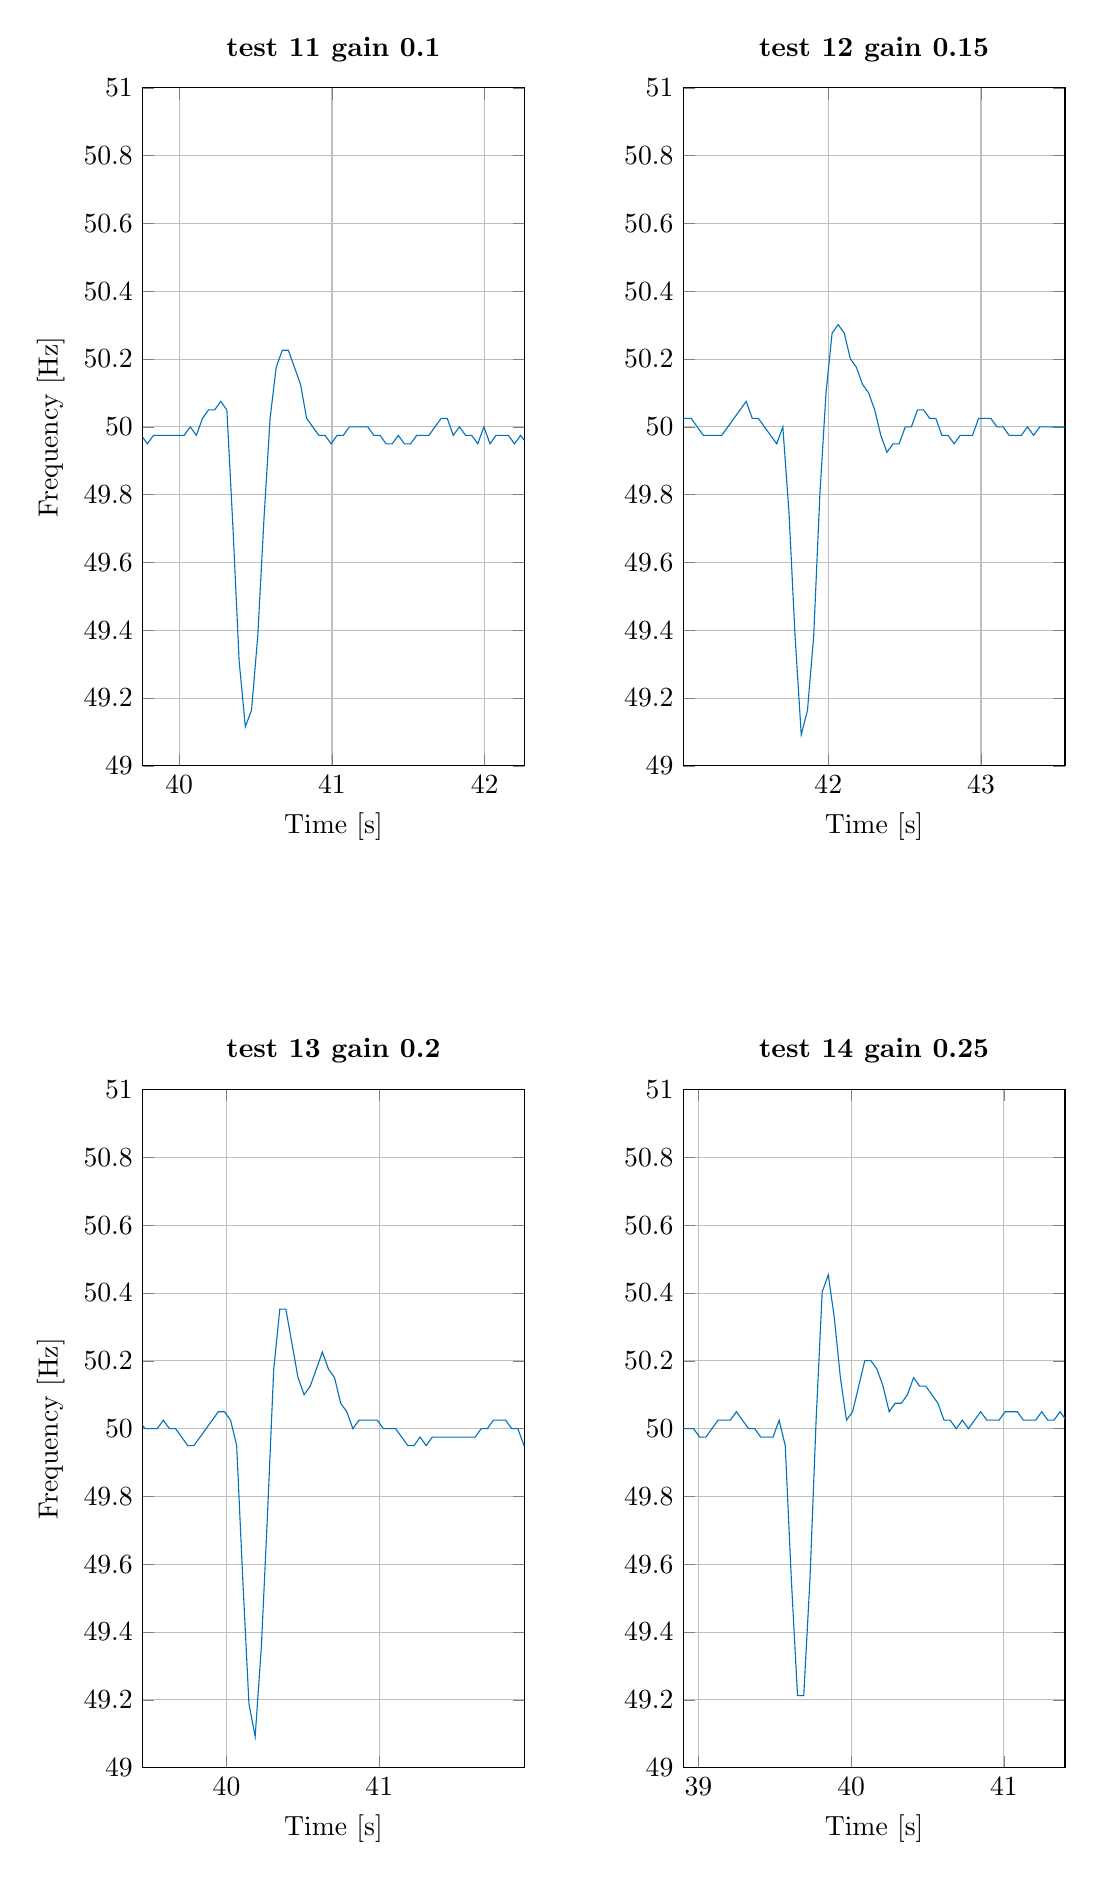
\begin{tikzpicture}

\begin{axis}[%
width=0.4\textwidth,
height=3.39in,
at={(1.297in,5.802in)},
scale only axis,
xmin=39.76,
xmax=42.26,
xlabel={Time [s]},
xmajorgrids,
ymin=49,
ymax=51,
ylabel={Frequency [Hz]},
ymajorgrids,
axis background/.style={fill=white},
title style={font=\bfseries},
title={test 11 gain 0.1}
]
\addplot [color=mycolor1,solid,forget plot]
  table[row sep=crcr]{%
39.75198	49.9750124937551\\
39.792	49.950049950044\\
39.83204	49.9750124937551\\
39.87206	49.9750124937551\\
39.91208	49.9750124937551\\
39.9521	49.9750124937463\\
39.99212	49.9750124937551\\
40.03214	49.9750124937551\\
40.07216	50.0000000000011\\
40.11216	49.9750124937551\\
40.15218	50.0250125062532\\
40.19216	50.0500500500492\\
40.23212	50.0500500500492\\
40.27208	50.0751126690017\\
40.31202	50.0500500500492\\
40.35198	49.701789264417\\
40.39222	49.309664694281\\
40.43278	49.1159135559918\\
40.4735	49.1642084562416\\
40.51418	49.3827160493808\\
40.55468	49.7265042267554\\
40.5949	50.0250125062532\\
40.63488	50.1756146512739\\
40.67474	50.2260170768472\\
40.71456	50.2260170768472\\
40.75438	50.1756146512828\\
40.79424	50.1253132832043\\
40.83414	50.0250125062532\\
40.87412	50.0000000000011\\
40.91412	49.9750124937551\\
40.95414	49.9750124937551\\
40.99416	49.950049950044\\
41.0342	49.9750124937551\\
41.07422	49.9750124937551\\
41.11424	50.0000000000011\\
41.15424	50.0000000000011\\
41.19424	49.9999999999922\\
41.23424	50.0000000000011\\
41.27424	49.9750124937551\\
41.31426	49.9750124937551\\
41.35428	49.9500499500529\\
41.39432	49.950049950044\\
41.43436	49.9750124937551\\
41.47438	49.9500499500529\\
41.51442	49.950049950044\\
41.55446	49.9750124937551\\
41.59448	49.9750124937551\\
41.6345	49.9750124937551\\
41.67452	50.0000000000011\\
41.71452	50.0250125062532\\
41.7545	50.0250125062532\\
41.79448	49.9750124937463\\
41.8345	50.0000000000011\\
41.8745	49.9750124937551\\
41.91452	49.9750124937551\\
41.95454	49.950049950044\\
41.99458	50.0000000000011\\
42.03458	49.9500499500529\\
42.07462	49.9750124937551\\
42.11464	49.9750124937463\\
42.15466	49.9750124937551\\
42.19468	49.9500499500529\\
42.23472	49.9750124937551\\
42.27474	49.950049950044\\
};
\end{axis}

\begin{axis}[%
width=0.4\textwidth,
height=3.39in,
at={(4in,5.802in)},
scale only axis,
xmin=41.05,
xmax=43.55,
xlabel={Time [s]},
xmajorgrids,
ymin=49,
ymax=51,
ymajorgrids,
axis background/.style={fill=white},
title style={font=\bfseries},
title={test 12  gain 0.15}
]
\addplot [color=mycolor1,solid,forget plot]
  table[row sep=crcr]{%
41.02254	50.0250125062532\\
41.06252	50.0250125062532\\
41.1025	50.0250125062532\\
41.14248	50.0000000000011\\
41.18248	49.9750124937551\\
41.2225	49.9750124937551\\
41.26252	49.9750124937551\\
41.30254	49.9750124937463\\
41.34256	50.0000000000011\\
41.38256	50.0250125062532\\
41.42254	50.0500500500492\\
41.4625	50.0751126690106\\
41.50244	50.0250125062444\\
41.54242	50.0250125062532\\
41.5824	50.0000000000011\\
41.6224	49.9750124937551\\
41.66242	49.9500499500529\\
41.70246	50.0000000000011\\
41.74246	49.7512437810962\\
41.78266	49.3827160493808\\
41.82316	49.0918016691218\\
41.8639	49.1642084562416\\
41.90458	49.3827160493808\\
41.94508	49.8007968127488\\
41.98524	50.1002004007989\\
42.02516	50.2765208647647\\
42.06494	50.3018108651897\\
42.1047	50.2765208647557\\
42.14448	50.2008032128448\\
42.18432	50.1756146512828\\
42.22418	50.1253132832133\\
42.26408	50.1002004007989\\
42.304	50.0500500500492\\
42.34396	49.9750124937551\\
42.38398	49.9251123314978\\
42.42404	49.9500499500529\\
42.46408	49.9500499500529\\
42.50412	49.9999999999922\\
42.54412	50.0000000000011\\
42.58412	50.0500500500492\\
42.62408	50.0500500500581\\
42.66404	50.0250125062532\\
42.70402	50.0250125062444\\
42.744	49.9750124937551\\
42.78402	49.9750124937551\\
42.82404	49.9500499500529\\
42.86408	49.9750124937463\\
42.9041	49.9750124937551\\
42.94412	49.9750124937551\\
42.98414	50.0250125062532\\
43.02412	50.0250125062532\\
43.0641	50.0250125062532\\
43.10408	50.0000000000011\\
43.14408	50.0000000000011\\
43.18408	49.9750124937551\\
43.2241	49.9750124937463\\
43.26412	49.9750124937551\\
43.30414	50.0000000000011\\
43.34414	49.9750124937551\\
43.38416	50.0000000000011\\
43.42416	49.9999999999922\\
43.46416	50.0000000000011\\
43.50416	50.0000000000011\\
43.54416	50.0000000000011\\
43.58416	50.0000000000011\\
};
\end{axis}

\begin{axis}[%
width=0.4\textwidth,
height=3.39in,
at={(1.297in,0.793in)},
scale only axis,
xmin=39.45,
xmax=41.95,
xlabel={Time [s]},
xmajorgrids,
ymin=49,
ymax=51,
ylabel={Frequency [Hz]},
ymajorgrids,
axis background/.style={fill=white},
title style={font=\bfseries},
title={test 13  gain 0.2}
]
\addplot [color=mycolor1,solid,forget plot]
  table[row sep=crcr]{%
39.42622	50.0250125062532\\
39.4662	49.9999999999922\\
39.5062	50.0000000000011\\
39.5462	50.0000000000011\\
39.5862	50.0250125062532\\
39.62618	50.0000000000011\\
39.66618	50.0000000000011\\
39.70618	49.9750124937551\\
39.7462	49.950049950044\\
39.78624	49.9500499500529\\
39.82628	49.9750124937551\\
39.8663	50.0000000000011\\
39.9063	50.0250125062532\\
39.94628	50.0500500500492\\
39.98624	50.0500500500492\\
40.0262	50.0250125062532\\
40.06618	49.9500499500529\\
40.10622	49.5540138751242\\
40.14658	49.1883915395935\\
40.18724	49.0918016691218\\
40.22798	49.3583415597226\\
40.2685	49.7512437810962\\
40.3087	50.1756146512739\\
40.34856	50.3524672709019\\
40.38828	50.3524672708929\\
40.428	50.2512562814075\\
40.4678	50.1504513540665\\
40.50768	50.1002004007989\\
40.5476	50.1253132832043\\
40.5875	50.1756146512828\\
40.62736	50.2260170768472\\
40.66718	50.1756146512739\\
40.70704	50.1504513540665\\
40.74692	50.0751126690017\\
40.78686	50.0500500500492\\
40.82682	50.0000000000011\\
40.86682	50.0250125062532\\
40.9068	50.0250125062532\\
40.94678	50.0250125062532\\
40.98676	50.0250125062532\\
41.02674	50.0000000000011\\
41.06674	50.0000000000011\\
41.10674	50.0000000000011\\
41.14674	49.9750124937463\\
41.18676	49.9500499500529\\
41.2268	49.9500499500529\\
41.26684	49.9750124937551\\
41.30686	49.950049950044\\
41.3469	49.9750124937551\\
41.38692	49.9750124937551\\
41.42694	49.9750124937551\\
41.46696	49.9750124937463\\
41.50698	49.9750124937551\\
41.547	49.9750124937551\\
41.58702	49.9750124937551\\
41.62704	49.9750124937463\\
41.66706	50.0000000000011\\
41.70706	50.0000000000011\\
41.74706	50.0250125062532\\
41.78704	50.0250125062532\\
41.82702	50.0250125062532\\
41.867	50.0000000000011\\
41.907	50.0000000000011\\
41.947	49.9500499500529\\
41.98704	49.950049950044\\
};
\end{axis}

\begin{axis}[%
width=0.4\textwidth,
height=3.39in,
at={(4in,0.793in)},
scale only axis,
xmin=38.9,
xmax=41.4,
xlabel={Time [s]},
xmajorgrids,
ymin=49,
ymax=51,
ymajorgrids,
axis background/.style={fill=white},
title style={font=\bfseries},
title={test 14  gain 0.25}
]
\addplot [color=mycolor1,solid,forget plot]
  table[row sep=crcr]{%
38.8884	50.0000000000011\\
38.9284	50.0000000000011\\
38.9684	50.0000000000011\\
39.0084	49.9750124937463\\
39.04842	49.9750124937551\\
39.08844	50.0000000000011\\
39.12844	50.0250125062532\\
39.16842	50.0250125062532\\
39.2084	50.0250125062532\\
39.24838	50.0500500500492\\
39.28834	50.0250125062532\\
39.32832	50.0000000000011\\
39.36832	50.0000000000011\\
39.40832	49.9750124937551\\
39.44834	49.9750124937551\\
39.48836	49.9750124937463\\
39.52838	50.0250125062532\\
39.56836	49.9500499500529\\
39.6084	49.5540138751242\\
39.64876	49.2125984251928\\
39.6894	49.2125984252014\\
39.73004	49.5540138751242\\
39.7704	50.0250125062532\\
39.81038	50.4032258064463\\
39.85006	50.4540867810311\\
39.8897	50.3271263210847\\
39.92944	50.1504513540665\\
39.96932	50.0250125062532\\
40.0093	50.0500500500492\\
40.04926	50.1253132832043\\
40.08916	50.2008032128538\\
40.129	50.2008032128538\\
40.16884	50.1756146512828\\
40.2087	50.1253132832043\\
40.2486	50.0500500500492\\
40.28856	50.0751126690017\\
40.3285	50.0751126690017\\
40.36844	50.1002004008078\\
40.40836	50.1504513540575\\
40.44824	50.1253132832133\\
40.48814	50.1253132832043\\
40.52804	50.1002004007989\\
40.56796	50.0751126690106\\
40.6079	50.0250125062532\\
40.64788	50.0250125062532\\
40.68786	49.9999999999922\\
40.72786	50.0250125062532\\
40.76784	50.0000000000011\\
40.80784	50.0250125062532\\
40.84782	50.0500500500492\\
40.88778	50.0250125062532\\
40.92776	50.0250125062532\\
40.96774	50.0250125062532\\
41.00772	50.0500500500492\\
41.04768	50.0500500500581\\
41.08764	50.0500500500492\\
41.1276	50.0250125062532\\
41.16758	50.0250125062532\\
41.20756	50.0250125062532\\
41.24754	50.0500500500492\\
41.2875	50.0250125062532\\
41.32748	50.0250125062532\\
41.36746	50.0500500500492\\
41.40742	50.0250125062532\\
};
\end{axis}
\end{tikzpicture}%
\caption{Step from 20 to 30 kW load, with various scaling factors.}
\label{fig:test11-14-20to30kwstepfreq}
\end{figure}

\begin{figure}[H]
\centering
% This file was created by matlab2tikz.
%
%The latest updates can be retrieved from
%  http://www.mathworks.com/matlabcentral/fileexchange/22022-matlab2tikz-matlab2tikz
%where you can also make suggestions and rate matlab2tikz.
%
\definecolor{mycolor1}{rgb}{0.00000,0.44700,0.74100}%
%
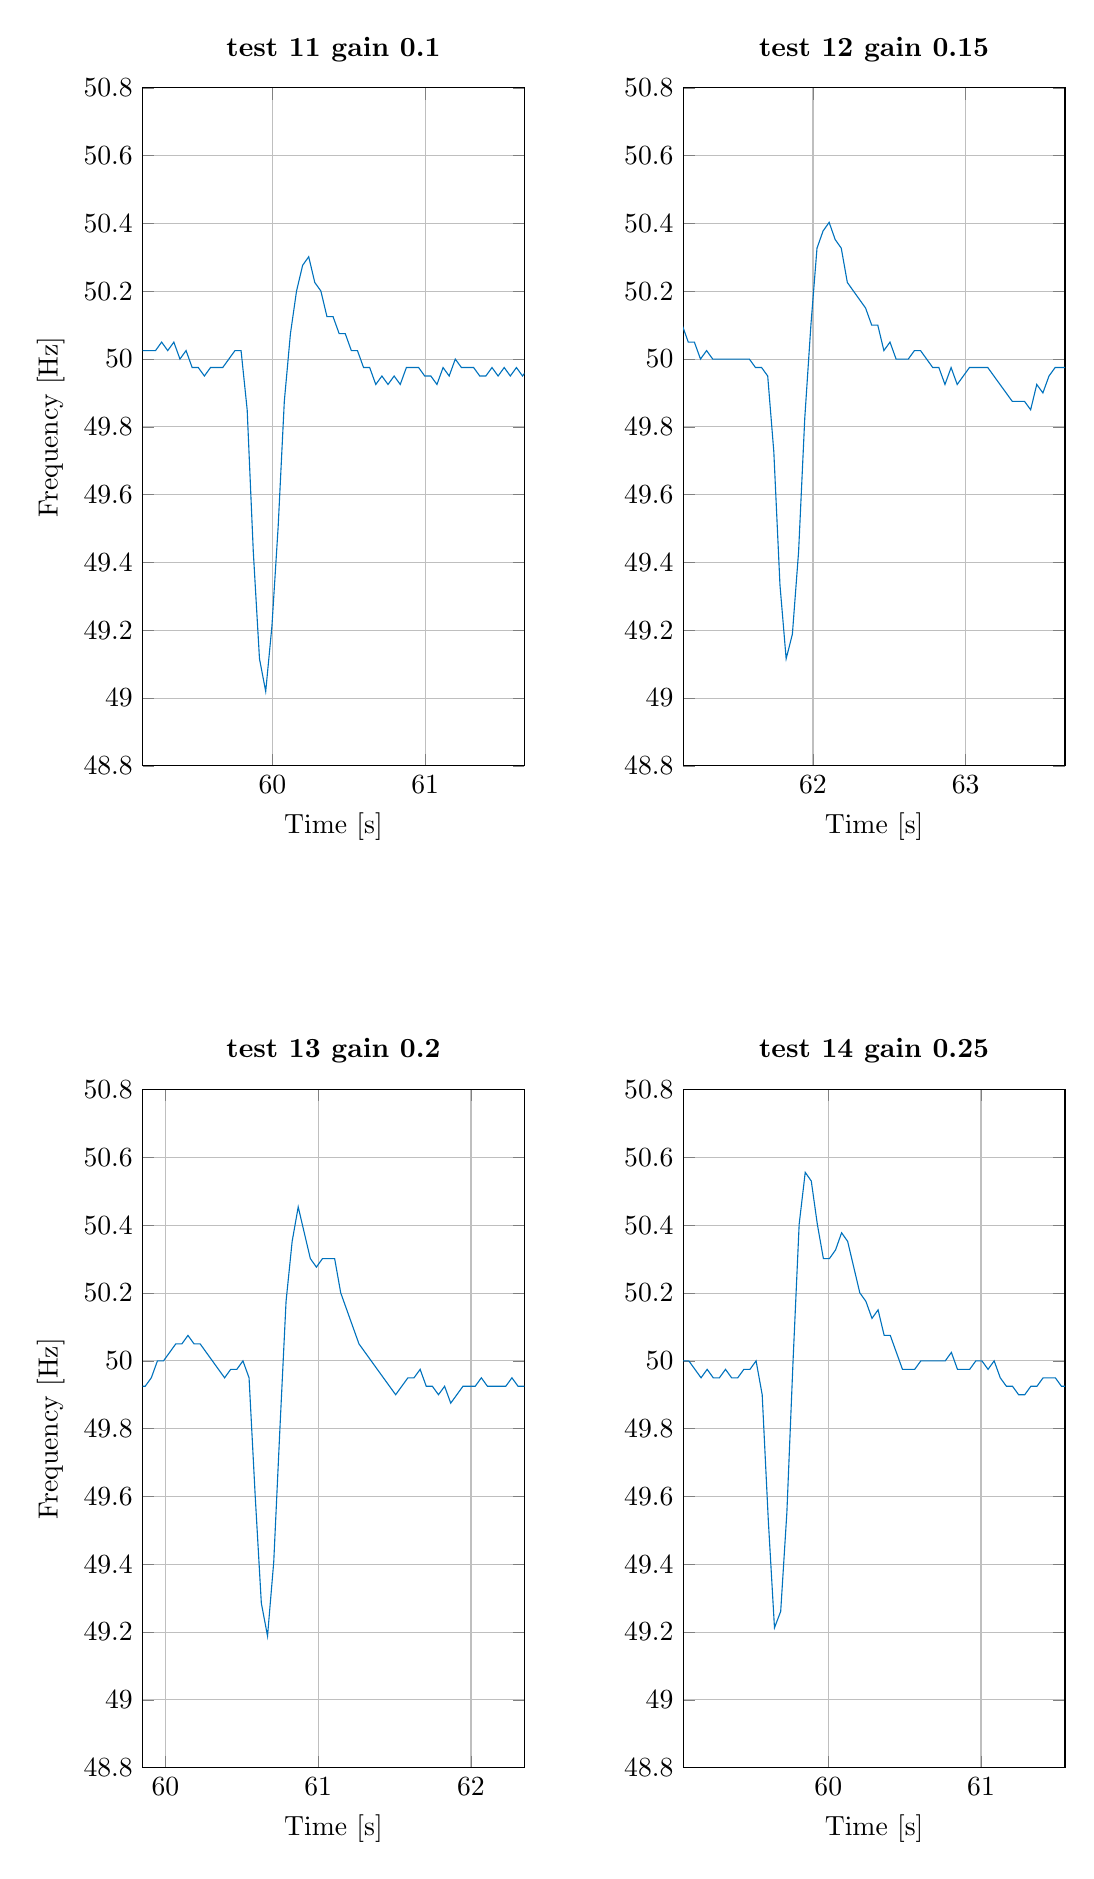
\begin{tikzpicture}

\begin{axis}[%
width=0.4\textwidth,
height=3.39in,
at={(1.297in,5.802in)},
scale only axis,
xmin=59.15,
xmax=61.65,
xlabel={Time [s]},
xmajorgrids,
ymin=48.8,
ymax=50.8,
ylabel={Frequency [Hz]},
ymajorgrids,
axis background/.style={fill=white},
title style={font=\bfseries},
title={test 11 gain 0.1}
]
\addplot [color=mycolor1,solid,forget plot]
  table[row sep=crcr]{%
59.11502	50.0250125062532\\
59.155	50.0250125062532\\
59.19498	50.0250125062532\\
59.23496	50.0250125062532\\
59.27494	50.0500500500492\\
59.3149	50.0250125062532\\
59.35488	50.0500500500492\\
59.39484	50.0000000000011\\
59.43484	50.0250125062532\\
59.47482	49.9750124937551\\
59.51484	49.9750124937463\\
59.55486	49.9500499500529\\
59.5949	49.9750124937551\\
59.63492	49.9750124937551\\
59.67494	49.9750124937463\\
59.71496	50.0000000000011\\
59.75496	50.0250125062532\\
59.79494	50.0250125062532\\
59.83492	49.8504486540446\\
59.87504	49.431537320807\\
59.9155	49.1159135559918\\
59.95622	49.0196078431405\\
59.99702	49.2125984251928\\
60.03766	49.5049504950517\\
60.07806	49.8753117206952\\
60.11816	50.0751126690017\\
60.1581	50.2008032128538\\
60.19794	50.2765208647557\\
60.23772	50.3018108651897\\
60.27748	50.2260170768472\\
60.3173	50.2008032128538\\
60.35714	50.1253132832043\\
60.39704	50.1253132832133\\
60.43694	50.0751126690017\\
60.47688	50.0751126690017\\
60.51682	50.0250125062532\\
60.5568	50.0250125062532\\
60.59678	49.9750124937551\\
60.6368	49.9750124937551\\
60.67682	49.9251123314978\\
60.71688	49.9500499500529\\
60.75692	49.9251123314978\\
60.79698	49.9500499500529\\
60.83702	49.9251123315066\\
60.87708	49.9750124937463\\
60.9171	49.9750124937551\\
60.95712	49.9750124937551\\
60.99714	49.9500499500529\\
61.03718	49.950049950044\\
61.07722	49.9251123315066\\
61.11728	49.9750124937551\\
61.1573	49.950049950044\\
61.19734	50.0000000000011\\
61.23734	49.9750124937551\\
61.27736	49.9750124937551\\
61.31738	49.9750124937551\\
61.3574	49.950049950044\\
61.39744	49.9500499500529\\
61.43748	49.9750124937551\\
61.4775	49.950049950044\\
61.51754	49.9750124937551\\
61.55756	49.9500499500529\\
61.5976	49.9750124937551\\
61.63762	49.950049950044\\
61.67766	49.9750124937551\\
};
\end{axis}

\begin{axis}[%
width=0.4\textwidth,
height=3.39in,
at={(4in,5.802in)},
scale only axis,
xmin=61.15,
xmax=63.65,
xlabel={Time [s]},
xmajorgrids,
ymin=48.8,
ymax=50.8,
ymajorgrids,
axis background/.style={fill=white},
title style={font=\bfseries},
title={test 12  gain 0.15}
]
\addplot [color=mycolor1,solid,forget plot]
  table[row sep=crcr]{%
61.1437	50.1002004007989\\
61.18362	50.0500500500581\\
61.22358	50.0500500500492\\
61.26354	49.9999999999922\\
61.30354	50.0250125062532\\
61.34352	50.0000000000011\\
61.38352	50.0000000000011\\
61.42352	50.0000000000011\\
61.46352	50.0000000000011\\
61.50352	50.0000000000011\\
61.54352	50.0000000000011\\
61.58352	50.0000000000011\\
61.62352	49.9750124937463\\
61.66354	49.9750124937551\\
61.70356	49.9500499500529\\
61.7436	49.7265042267554\\
61.78382	49.3339911198816\\
61.82436	49.1159135559918\\
61.86508	49.1883915395935\\
61.90574	49.431537320807\\
61.9462	49.8256103637346\\
61.98634	50.1002004007989\\
62.02626	50.3271263210847\\
62.066	50.3778337531533\\
62.1057	50.4032258064463\\
62.14538	50.3524672709019\\
62.1851	50.3271263210847\\
62.22484	50.2260170768472\\
62.26466	50.2008032128448\\
62.3045	50.1756146512828\\
62.34436	50.1504513540665\\
62.38424	50.1002004007989\\
62.42416	50.1002004007989\\
62.46408	50.0250125062532\\
62.50406	50.0500500500492\\
62.54402	50.0000000000011\\
62.58402	50.0000000000011\\
62.62402	50.0000000000011\\
62.66402	50.0250125062532\\
62.704	50.0250125062532\\
62.74398	50.0000000000011\\
62.78398	49.9750124937551\\
62.824	49.9750124937463\\
62.86402	49.9251123315066\\
62.90408	49.9750124937551\\
62.9441	49.9251123314978\\
62.98416	49.9500499500529\\
63.0242	49.9750124937551\\
63.06422	49.9750124937463\\
63.10424	49.9750124937551\\
63.14426	49.9750124937551\\
63.18428	49.9500499500529\\
63.22432	49.9251123314978\\
63.26438	49.9001996008032\\
63.30446	49.8753117206952\\
63.34456	49.8753117206952\\
63.38466	49.875311720704\\
63.42476	49.8504486540358\\
63.46488	49.9251123314978\\
63.50494	49.9001996008032\\
63.54502	49.9500499500529\\
63.58506	49.9750124937463\\
63.62508	49.9750124937551\\
63.6651	49.9750124937551\\
};
\end{axis}

\begin{axis}[%
width=0.4\textwidth,
height=3.39in,
at={(1.297in,0.793in)},
scale only axis,
xmin=59.85,
xmax=62.35,
xlabel={Time [s]},
xmajorgrids,
ymin=48.8,
ymax=50.8,
ylabel={Frequency [Hz]},
ymajorgrids,
axis background/.style={fill=white},
title style={font=\bfseries},
title={test 13  gain 0.2}
]
\addplot [color=mycolor1,solid,forget plot]
  table[row sep=crcr]{%
59.82724	49.9251123315066\\
59.8673	49.9251123314978\\
59.90736	49.9500499500529\\
59.9474	50.0000000000011\\
59.9874	50.0000000000011\\
60.0274	50.0250125062532\\
60.06738	50.0500500500492\\
60.10734	50.0500500500492\\
60.1473	50.0751126690017\\
60.18724	50.0500500500492\\
60.2272	50.0500500500492\\
60.26716	50.0250125062532\\
60.30714	50.0000000000011\\
60.34714	49.9750124937551\\
60.38716	49.9500499500529\\
60.4272	49.9750124937463\\
60.46722	49.9750124937551\\
60.50724	50.0000000000011\\
60.54724	49.9500499500529\\
60.58728	49.6031746031731\\
60.6276	49.2853622474143\\
60.66818	49.1883915395935\\
60.70884	49.4071146245031\\
60.74932	49.8007968127488\\
60.78948	50.1756146512828\\
60.82934	50.3524672708929\\
60.86906	50.4540867810311\\
60.9087	50.3778337531533\\
60.9484	50.3018108651897\\
60.98816	50.2765208647557\\
61.02794	50.3018108651897\\
61.0677	50.3018108651897\\
61.10746	50.3018108651897\\
61.14722	50.2008032128538\\
61.18706	50.1504513540665\\
61.22694	50.1002004007989\\
61.26686	50.0500500500492\\
61.30682	50.0250125062532\\
61.3468	50.0000000000011\\
61.3868	49.9750124937551\\
61.42682	49.950049950044\\
61.46686	49.9251123315066\\
61.50692	49.9001996007944\\
61.547	49.9251123315066\\
61.58706	49.9500499500529\\
61.6271	49.950049950044\\
61.66714	49.9750124937551\\
61.70716	49.9251123315066\\
61.74722	49.9251123314978\\
61.78728	49.9001996008032\\
61.82736	49.9251123314978\\
61.86742	49.8753117206952\\
61.90752	49.9001996008032\\
61.9476	49.9251123315066\\
61.98766	49.9251123314978\\
62.02772	49.9251123315066\\
62.06778	49.950049950044\\
62.10782	49.9251123315066\\
62.14788	49.9251123314978\\
62.18794	49.9251123315066\\
62.228	49.9251123315066\\
62.26806	49.950049950044\\
62.3081	49.9251123315066\\
62.34816	49.9251123314978\\
62.38822	49.9251123315066\\
};
\end{axis}

\begin{axis}[%
width=0.4\textwidth,
height=3.39in,
at={(4in,0.793in)},
scale only axis,
xmin=59.05,
xmax=61.55,
xlabel={Time [s]},
xmajorgrids,
ymin=48.8,
ymax=50.8,
ymajorgrids,
axis background/.style={fill=white},
title style={font=\bfseries},
title={test 14  gain 0.25}
]
\addplot [color=mycolor1,solid,forget plot]
  table[row sep=crcr]{%
59.04718	50.0000000000011\\
59.08718	50.0000000000011\\
59.12718	49.9750124937551\\
59.1672	49.9500499500529\\
59.20724	49.9750124937463\\
59.24726	49.9500499500529\\
59.2873	49.9500499500529\\
59.32734	49.9750124937463\\
59.36736	49.9500499500529\\
59.4074	49.9500499500529\\
59.44744	49.9750124937551\\
59.48746	49.9750124937463\\
59.52748	50.0000000000011\\
59.56748	49.9001996008032\\
59.60756	49.5294700346719\\
59.64794	49.2125984251928\\
59.68858	49.2610837438451\\
59.72918	49.5540138751242\\
59.76954	50.0000000000011\\
59.80954	50.4032258064463\\
59.84922	50.5561172901901\\
59.88878	50.5305709954512\\
59.92836	50.4032258064554\\
59.96804	50.3018108651897\\
60.0078	50.3018108651897\\
60.04756	50.3271263210937\\
60.0873	50.3778337531443\\
60.127	50.3524672708929\\
60.16672	50.2765208647647\\
60.2065	50.2008032128448\\
60.24634	50.1756146512828\\
60.2862	50.1253132832043\\
60.3261	50.1504513540665\\
60.36598	50.0751126690017\\
60.40592	50.0751126690017\\
60.44586	50.0250125062532\\
60.48584	49.9750124937551\\
60.52586	49.9750124937551\\
60.56588	49.9750124937551\\
60.6059	49.9999999999922\\
60.6459	50.0000000000011\\
60.6859	50.0000000000011\\
60.7259	50.0000000000011\\
60.7659	50.0000000000011\\
60.8059	50.0250125062532\\
60.84588	49.9750124937551\\
60.8859	49.9750124937463\\
60.92592	49.9750124937551\\
60.96594	50.0000000000011\\
61.00594	50.0000000000011\\
61.04594	49.9750124937551\\
61.08596	50.0000000000011\\
61.12596	49.950049950044\\
61.166	49.9251123315066\\
61.20606	49.9251123314978\\
61.24612	49.9001996008032\\
61.2862	49.9001996007944\\
61.32628	49.9251123315066\\
61.36634	49.9251123314978\\
61.4064	49.9500499500529\\
61.44644	49.9500499500529\\
61.48648	49.950049950044\\
61.52652	49.9251123315066\\
61.56658	49.9251123315066\\
};
\end{axis}
\end{tikzpicture}%
\caption{Step from 30 to 40 kW load, with various scaling factors.}
\label{fig:test11-14-30to40kwstepfreq}
\end{figure}

\begin{figure}[H]
\centering
% This file was created by matlab2tikz.
%
%The latest updates can be retrieved from
%  http://www.mathworks.com/matlabcentral/fileexchange/22022-matlab2tikz-matlab2tikz
%where you can also make suggestions and rate matlab2tikz.
%
\definecolor{mycolor1}{rgb}{0.00000,0.44700,0.74100}%
%
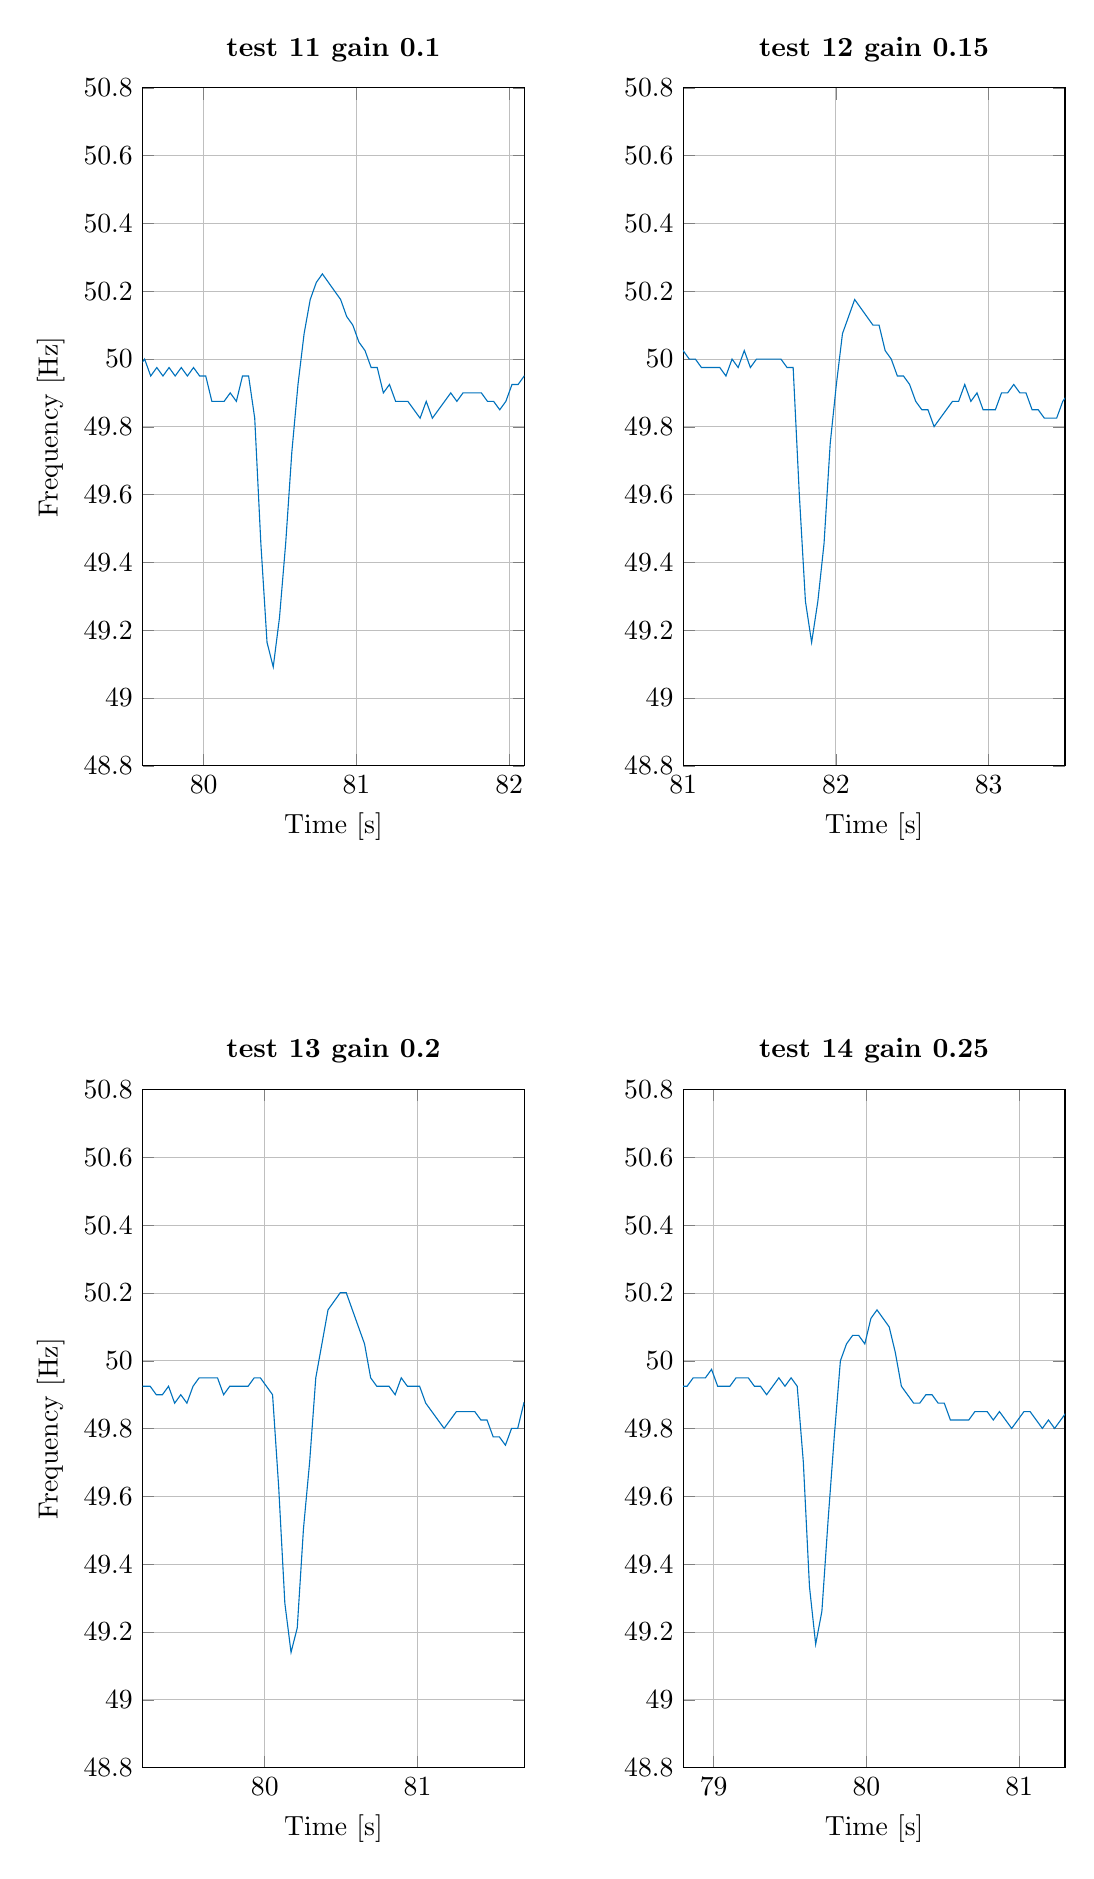
\begin{tikzpicture}

\begin{axis}[%
width=0.4\textwidth,
height=3.39in,
at={(1.297in,5.802in)},
scale only axis,
xmin=79.6,
xmax=82.1,
xlabel={Time [s]},
xmajorgrids,
ymin=48.8,
ymax=50.8,
ylabel={Frequency [Hz]},
ymajorgrids,
axis background/.style={fill=white},
title style={font=\bfseries},
title={test 11 gain 0.1}
]
\addplot [color=mycolor1,solid,forget plot]
  table[row sep=crcr]{%
79.57342	49.9750124937551\\
79.61344	50.0000000000099\\
79.65344	49.950049950044\\
79.69348	49.9750124937551\\
79.7335	49.950049950044\\
79.77354	49.9750124937551\\
79.81356	49.9500499500618\\
79.8536	49.9750124937374\\
79.89362	49.9500499500618\\
79.93366	49.9750124937551\\
79.97368	49.950049950044\\
80.01372	49.950049950044\\
80.05376	49.875311720704\\
80.09386	49.875311720704\\
80.13396	49.8753117206863\\
80.17406	49.9001996008121\\
80.21414	49.8753117206863\\
80.25424	49.9500499500618\\
80.29428	49.950049950044\\
80.33432	49.825610363717\\
80.37446	49.4559841740978\\
80.4149	49.1642084562331\\
80.45558	49.0918016691218\\
80.49632	49.2368291482151\\
80.53694	49.4559841740804\\
80.57738	49.7265042267466\\
80.6176	49.9251123315066\\
80.65766	50.0751126690017\\
80.6976	50.1756146512739\\
80.73746	50.2260170768562\\
80.77728	50.2512562814075\\
80.81708	50.2260170768383\\
80.8569	50.2008032128538\\
80.89674	50.1756146512739\\
80.9366	50.1253132832222\\
80.9765	50.10020040079\\
81.01642	50.0500500500581\\
81.05638	50.0250125062532\\
81.09636	49.9750124937551\\
81.13638	49.9750124937551\\
81.1764	49.9001996007944\\
81.21648	49.9251123315066\\
81.25654	49.8753117206863\\
81.29664	49.875311720704\\
81.33674	49.875311720704\\
81.37684	49.8504486540358\\
81.41696	49.825610363717\\
81.4571	49.875311720704\\
81.4972	49.8256103637346\\
81.53734	49.8504486540358\\
81.57746	49.8753117206863\\
81.61756	49.9001996008121\\
81.65764	49.8753117206863\\
81.69774	49.9001996007944\\
81.73782	49.9001996008121\\
81.7779	49.9001996007944\\
81.81798	49.9001996007944\\
81.85806	49.875311720704\\
81.89816	49.8753117206863\\
81.93826	49.8504486540534\\
81.97838	49.8753117206863\\
82.01848	49.9251123315066\\
82.05854	49.9251123315066\\
82.0986	49.950049950044\\
82.13864	49.9500499500618\\
};
\end{axis}

\begin{axis}[%
width=0.4\textwidth,
height=3.39in,
at={(4in,5.802in)},
scale only axis,
xmin=81,
xmax=83.5,
xlabel={Time [s]},
xmajorgrids,
ymin=48.8,
ymax=50.8,
ymajorgrids,
axis background/.style={fill=white},
title style={font=\bfseries},
title={test 12  gain 0.15}
]
\addplot [color=mycolor1,solid,forget plot]
  table[row sep=crcr]{%
80.96004	49.9999999999922\\
81.00004	50.0250125062532\\
81.04002	50.0000000000099\\
81.08002	49.9999999999922\\
81.12002	49.9750124937551\\
81.16004	49.9750124937551\\
81.20006	49.9750124937551\\
81.24008	49.9750124937551\\
81.2801	49.950049950044\\
81.32014	50.0000000000099\\
81.36014	49.9750124937374\\
81.40016	50.0250125062532\\
81.44014	49.9750124937551\\
81.48016	50.0000000000099\\
81.52016	49.9999999999922\\
81.56016	50.0000000000099\\
81.60016	49.9999999999922\\
81.64016	50.0000000000099\\
81.68016	49.9750124937374\\
81.72018	49.9750124937551\\
81.7602	49.6031746031818\\
81.80052	49.2853622474057\\
81.8411	49.1642084562502\\
81.88178	49.2853622474057\\
81.92236	49.4559841740978\\
81.9628	49.7512437810962\\
82.003	49.9251123314889\\
82.04306	50.0751126690017\\
82.083	50.1253132832222\\
82.1229	50.1756146512739\\
82.16276	50.1504513540665\\
82.20264	50.1253132832043\\
82.24254	50.1002004008078\\
82.28246	50.10020040079\\
82.32238	50.0250125062532\\
82.36236	50.0000000000099\\
82.40236	49.950049950044\\
82.4424	49.950049950044\\
82.48244	49.9251123315066\\
82.5225	49.875311720704\\
82.5626	49.8504486540358\\
82.60272	49.8504486540358\\
82.64284	49.8007968127488\\
82.683	49.8256103637346\\
82.72314	49.8504486540358\\
82.76326	49.8753117206863\\
82.80336	49.875311720704\\
82.84346	49.9251123315066\\
82.88352	49.8753117206863\\
82.92362	49.9001996008121\\
82.9637	49.8504486540358\\
83.00382	49.8504486540358\\
83.04394	49.8504486540358\\
83.08406	49.9001996007944\\
83.12414	49.9001996008121\\
83.16422	49.9251123314889\\
83.20428	49.9001996008121\\
83.24436	49.9001996007944\\
83.28444	49.8504486540358\\
83.32456	49.8504486540358\\
83.36468	49.8256103637346\\
83.40482	49.825610363717\\
83.44496	49.8256103637346\\
83.4851	49.8753117206863\\
83.5252	49.9001996008121\\
};
\end{axis}

\begin{axis}[%
width=0.4\textwidth,
height=3.39in,
at={(1.297in,0.793in)},
scale only axis,
xmin=79.2,
xmax=81.7,
xlabel={Time [s]},
xmajorgrids,
ymin=48.8,
ymax=50.8,
ylabel={Frequency [Hz]},
ymajorgrids,
axis background/.style={fill=white},
title style={font=\bfseries},
title={test 13  gain 0.2}
]
\addplot [color=mycolor1,solid,forget plot]
  table[row sep=crcr]{%
79.1698	49.9251123315066\\
79.20986	49.9251123315066\\
79.24992	49.9251123314889\\
79.28998	49.9001996008121\\
79.33006	49.9001996007944\\
79.37014	49.9251123315066\\
79.4102	49.8753117206863\\
79.4503	49.9001996008121\\
79.49038	49.8753117206863\\
79.53048	49.9251123315066\\
79.57054	49.950049950044\\
79.61058	49.9500499500618\\
79.65062	49.950049950044\\
79.69066	49.950049950044\\
79.7307	49.9001996008121\\
79.77078	49.9251123314889\\
79.81084	49.9251123315066\\
79.8509	49.9251123315066\\
79.89096	49.9251123315066\\
79.93102	49.950049950044\\
79.97106	49.950049950044\\
80.0111	49.9251123315066\\
80.05116	49.9001996007944\\
80.09124	49.6277915632905\\
80.13154	49.2853622474057\\
80.17212	49.1400491400479\\
80.21282	49.2125984252014\\
80.25346	49.504950495043\\
80.29386	49.701789264417\\
80.3341	49.950049950044\\
80.37414	50.0500500500581\\
80.4141	50.1504513540665\\
80.45398	50.1756146512739\\
80.49384	50.2008032128538\\
80.53368	50.2008032128538\\
80.57352	50.1504513540486\\
80.6134	50.1002004008078\\
80.65332	50.0500500500581\\
80.69328	49.950049950044\\
80.73332	49.9251123315066\\
80.77338	49.9251123314889\\
80.81344	49.9251123315066\\
80.8535	49.9001996008121\\
80.89358	49.950049950044\\
80.93362	49.9251123315066\\
80.97368	49.9251123314889\\
81.01374	49.9251123315066\\
81.0538	49.875311720704\\
81.0939	49.8504486540358\\
81.13402	49.8256103637346\\
81.17416	49.8007968127488\\
81.21432	49.825610363717\\
81.25446	49.8504486540358\\
81.29458	49.8504486540358\\
81.3347	49.8504486540358\\
81.37482	49.8504486540534\\
81.41494	49.825610363717\\
81.45508	49.8256103637346\\
81.49522	49.7760079641532\\
81.5354	49.7760079641708\\
81.57558	49.7512437810962\\
81.61578	49.8007968127488\\
81.65594	49.8007968127488\\
81.6961	49.8753117206863\\
81.7362	49.8504486540358\\
};
\end{axis}

\begin{axis}[%
width=0.4\textwidth,
height=3.39in,
at={(4in,0.793in)},
scale only axis,
xmin=78.8,
xmax=81.3,
xlabel={Time [s]},
xmajorgrids,
ymin=48.8,
ymax=50.8,
ymajorgrids,
axis background/.style={fill=white},
title style={font=\bfseries},
title={test 14  gain 0.25}
]
\addplot [color=mycolor1,solid,forget plot]
  table[row sep=crcr]{%
78.78574	49.9251123315066\\
78.8258	49.9251123314889\\
78.86586	49.9500499500618\\
78.9059	49.950049950044\\
78.94594	49.950049950044\\
78.98598	49.9750124937551\\
79.026	49.9251123315066\\
79.06606	49.9251123315066\\
79.10612	49.9251123315066\\
79.14618	49.950049950044\\
79.18622	49.950049950044\\
79.22626	49.9500499500618\\
79.2663	49.9251123314889\\
79.30636	49.9251123315066\\
79.34642	49.9001996007944\\
79.3865	49.9251123315066\\
79.42656	49.950049950044\\
79.4666	49.9251123315066\\
79.50666	49.9500499500618\\
79.5467	49.9251123314889\\
79.58676	49.701789264417\\
79.627	49.3339911198902\\
79.66754	49.1642084562331\\
79.70822	49.2610837438451\\
79.74882	49.5294700346719\\
79.7892	49.7760079641708\\
79.82938	49.9999999999922\\
79.86938	50.0500500500581\\
79.90934	50.0751126690017\\
79.94928	50.0751126690017\\
79.98922	50.0500500500403\\
80.02918	50.1253132832043\\
80.06908	50.1504513540665\\
80.10896	50.1253132832043\\
80.14886	50.1002004008078\\
80.18878	50.0250125062532\\
80.22876	49.9251123315066\\
80.26882	49.9001996007944\\
80.3089	49.875311720704\\
80.349	49.8753117206863\\
80.3891	49.9001996008121\\
80.42918	49.9001996007944\\
80.46926	49.875311720704\\
80.50936	49.8753117206863\\
80.54946	49.8256103637346\\
80.5896	49.825610363717\\
80.62974	49.8256103637346\\
80.66988	49.8256103637346\\
80.71002	49.8504486540358\\
80.75014	49.8504486540358\\
80.79026	49.8504486540358\\
80.83038	49.825610363717\\
80.87052	49.8504486540534\\
80.91064	49.825610363717\\
80.95078	49.8007968127488\\
80.99094	49.8256103637346\\
81.03108	49.8504486540358\\
81.0712	49.8504486540358\\
81.11132	49.8256103637346\\
81.15146	49.8007968127488\\
81.19162	49.825610363717\\
81.23176	49.8007968127488\\
81.27192	49.8256103637346\\
81.31206	49.8504486540358\\
};
\end{axis}
\end{tikzpicture}%
\caption{Step from 40 to 50 kW load, with various scaling factors.}
\label{fig:test11-14-40to50kwstepfreq}
\end{figure}

\begin{figure}[H]
\centering
% This file was created by matlab2tikz.
%
%The latest updates can be retrieved from
%  http://www.mathworks.com/matlabcentral/fileexchange/22022-matlab2tikz-matlab2tikz
%where you can also make suggestions and rate matlab2tikz.
%
\definecolor{mycolor1}{rgb}{0.00000,0.44700,0.74100}%
%
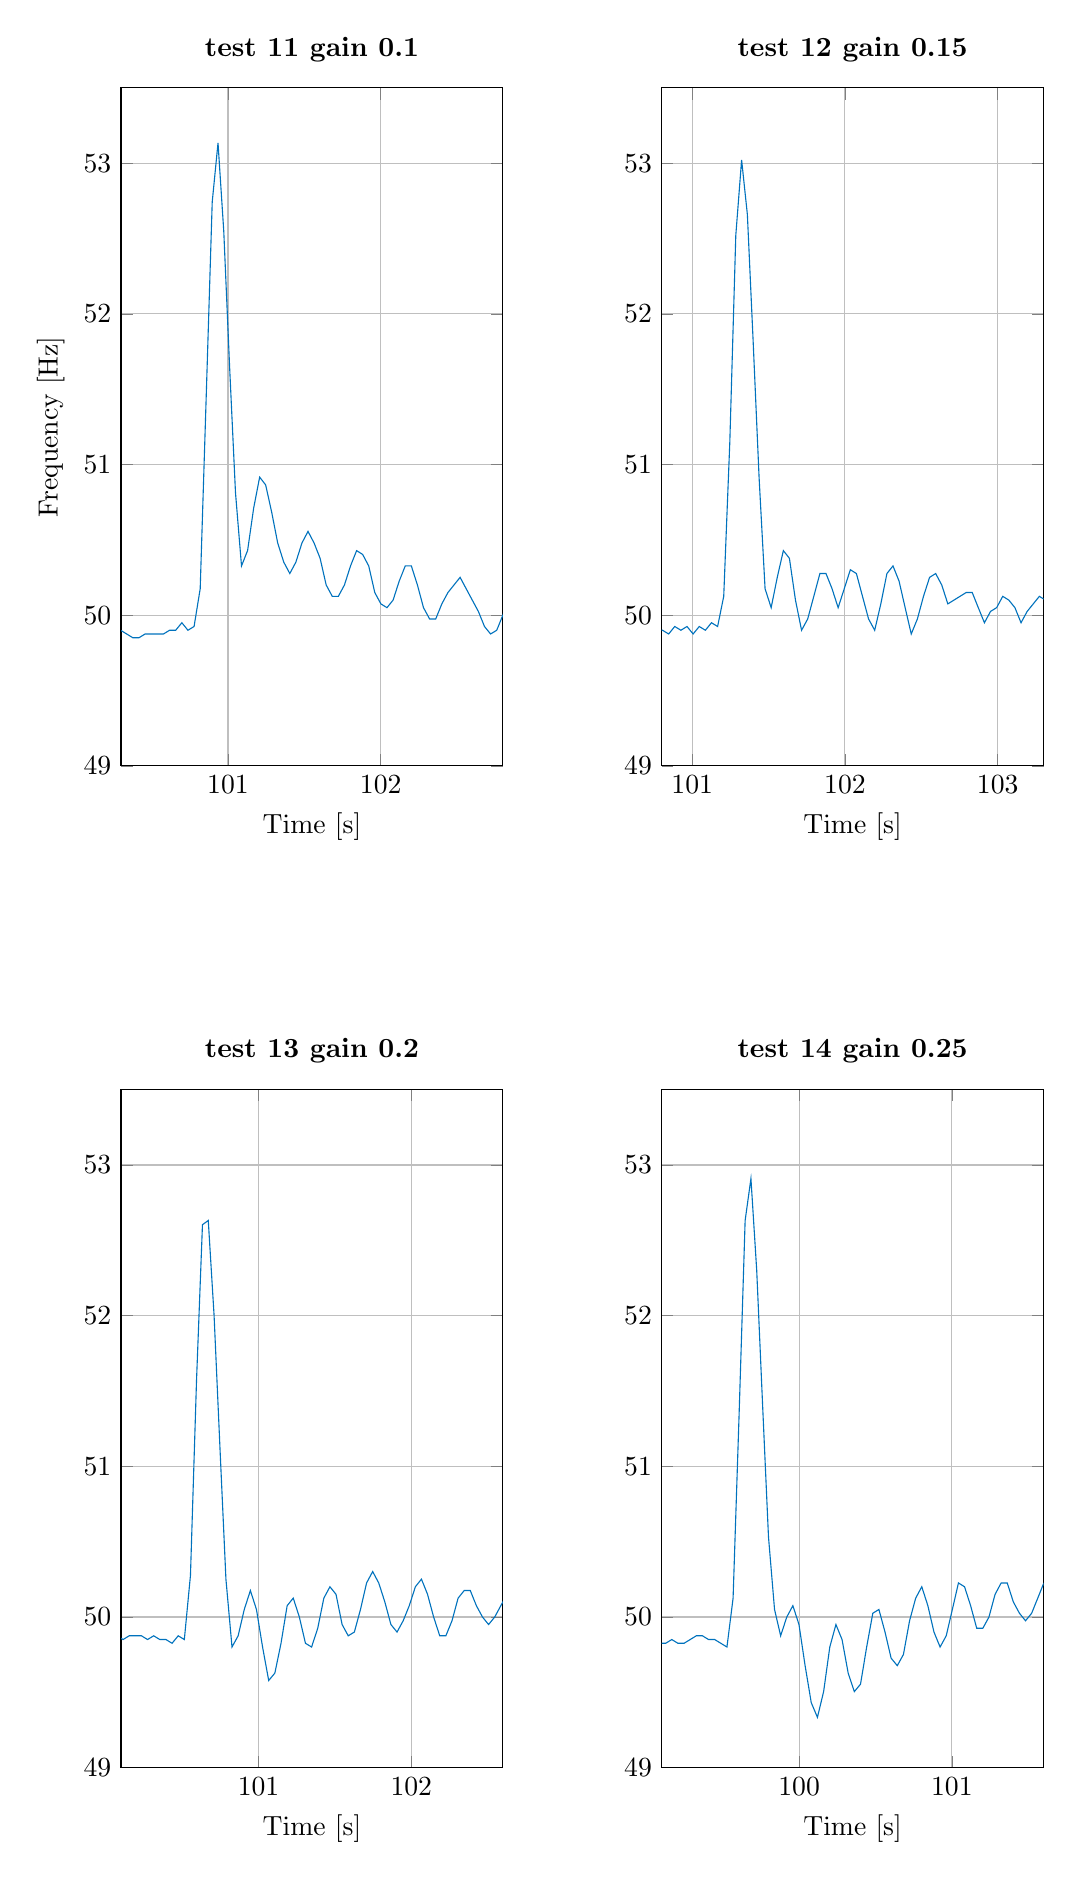
\begin{tikzpicture}

\begin{axis}[%
width=0.4\textwidth,
height=3.39in,
at={(1.297in,5.802in)},
scale only axis,
xmin=100.3,
xmax=102.8,
xlabel={Time [s]},
xmajorgrids,
ymin=49,
ymax=53.5,
ylabel={Frequency [Hz]},
ymajorgrids,
axis background/.style={fill=white},
title style={font=\bfseries},
title={test 11 gain 0.1}
]
\addplot [color=mycolor1,solid,forget plot]
  table[row sep=crcr]{%
100.29714	49.9001996008121\\
100.33722	49.8753117206863\\
100.37732	49.8504486540358\\
100.41744	49.8504486540358\\
100.45756	49.875311720704\\
100.49766	49.875311720704\\
100.53776	49.8753117206863\\
100.57786	49.875311720704\\
100.61796	49.9001996007944\\
100.65804	49.9001996008121\\
100.69812	49.950049950044\\
100.73816	49.9001996007944\\
100.77824	49.9251123315066\\
100.8183	50.1756146512739\\
100.85816	51.4668039114775\\
100.89702	52.7426160337556\\
100.93494	53.1349628055315\\
100.97258	52.5486074619001\\
101.01064	51.6528925619863\\
101.04936	50.8130081300786\\
101.08872	50.3271263210937\\
101.12846	50.4286434694935\\
101.16812	50.709939148056\\
101.20756	50.916496945022\\
101.24684	50.864699898266\\
101.28616	50.6842372022232\\
101.32562	50.47955577991\\
101.36524	50.3524672709109\\
101.40496	50.2765208647467\\
101.44474	50.3524672708929\\
101.48446	50.47955577991\\
101.52408	50.5561172901992\\
101.56364	50.47955577991\\
101.60326	50.3778337531533\\
101.64296	50.2008032128359\\
101.6828	50.1253132832222\\
101.7227	50.1253132832043\\
101.7626	50.2008032128538\\
101.80244	50.3271263210757\\
101.84218	50.4286434694935\\
101.88184	50.4032258064463\\
101.92152	50.3271263210937\\
101.96126	50.1504513540665\\
102.00114	50.0751126690017\\
102.04108	50.0500500500581\\
102.08104	50.10020040079\\
102.12096	50.2260170768562\\
102.16078	50.3271263210757\\
102.20052	50.3271263210937\\
102.24026	50.2008032128538\\
102.2801	50.0500500500403\\
102.32006	49.9750124937551\\
102.36008	49.9750124937551\\
102.4001	50.0751126690017\\
102.44004	50.1504513540665\\
102.47992	50.2008032128538\\
102.51976	50.2512562814075\\
102.55956	50.1756146512739\\
102.59942	50.1002004008078\\
102.63934	50.0250125062532\\
102.67932	49.9251123314889\\
102.71938	49.875311720704\\
102.75948	49.9001996007944\\
102.79956	50.0000000000099\\
102.83956	50.10020040079\\
};
\end{axis}

\begin{axis}[%
width=0.4\textwidth,
height=3.39in,
at={(4in,5.802in)},
scale only axis,
xmin=100.8,
xmax=103.3,
xlabel={Time [s]},
xmajorgrids,
ymin=49,
ymax=53.5,
ymajorgrids,
axis background/.style={fill=white},
title style={font=\bfseries},
title={test 12  gain 0.15}
]
\addplot [color=mycolor1,solid,forget plot]
  table[row sep=crcr]{%
100.76576	49.9001996008121\\
100.80584	49.9001996007944\\
100.84592	49.875311720704\\
100.88602	49.9251123314889\\
100.92608	49.9001996008121\\
100.96616	49.9251123314889\\
101.00622	49.875311720704\\
101.04632	49.9251123315066\\
101.08638	49.9001996007944\\
101.12646	49.950049950044\\
101.1665	49.9251123315066\\
101.20656	50.1253132832043\\
101.24646	51.1508951406773\\
101.28556	52.5210084033505\\
101.32364	53.022269353138\\
101.36136	52.6592943654492\\
101.39934	51.8134715025874\\
101.43794	50.916496945022\\
101.47722	50.1756146512739\\
101.51708	50.0500500500403\\
101.55704	50.2512562814075\\
101.59684	50.4286434694935\\
101.6365	50.3778337531533\\
101.6762	50.1002004008078\\
101.71612	49.9001996007944\\
101.7562	49.9750124937551\\
101.79622	50.1253132832043\\
101.83612	50.2765208647467\\
101.8759	50.2765208647647\\
101.91568	50.1756146512739\\
101.95554	50.0500500500581\\
101.9955	50.1756146512739\\
102.03536	50.3018108651897\\
102.07512	50.2765208647647\\
102.1149	50.1253132832043\\
102.1548	49.9750124937551\\
102.19482	49.9001996007944\\
102.2349	50.0751126690017\\
102.27484	50.2765208647647\\
102.31462	50.3271263210757\\
102.35436	50.2260170768562\\
102.39418	50.0500500500403\\
102.43414	49.875311720704\\
102.47424	49.9750124937551\\
102.51426	50.1253132832043\\
102.55416	50.2512562814075\\
102.59396	50.2765208647647\\
102.63374	50.2008032128359\\
102.67358	50.0751126690195\\
102.71352	50.10020040079\\
102.75344	50.1253132832043\\
102.79334	50.1504513540665\\
102.83322	50.1504513540665\\
102.8731	50.0500500500581\\
102.91306	49.950049950044\\
102.9531	50.0250125062532\\
102.99308	50.0500500500403\\
103.03304	50.1253132832222\\
103.07294	50.10020040079\\
103.11286	50.0500500500581\\
103.15282	49.950049950044\\
103.19286	50.0250125062532\\
103.23284	50.0751126690017\\
103.27278	50.1253132832043\\
103.31268	50.1002004008078\\
};
\end{axis}

\begin{axis}[%
width=0.4\textwidth,
height=3.39in,
at={(1.297in,0.793in)},
scale only axis,
xmin=100.1,
xmax=102.6,
xlabel={Time [s]},
xmajorgrids,
ymin=49,
ymax=53.5,
ymajorgrids,
axis background/.style={fill=white},
title style={font=\bfseries},
title={test 13  gain 0.2}
]
\addplot [color=mycolor1,solid,forget plot]
  table[row sep=crcr]{%
100.07324	49.875311720704\\
100.11334	49.8504486540358\\
100.15346	49.875311720704\\
100.19356	49.8753117206863\\
100.23366	49.875311720704\\
100.27376	49.8504486540358\\
100.31388	49.875311720704\\
100.35398	49.8504486540358\\
100.3941	49.8504486540358\\
100.43422	49.8256103637346\\
100.47436	49.8753117206863\\
100.51446	49.8504486540358\\
100.55458	50.2765208647647\\
100.59436	51.5729757606978\\
100.63314	52.6038926880547\\
100.67116	52.631578947373\\
100.70916	52.0020800832025\\
100.74762	51.1247443762821\\
100.78674	50.2512562814075\\
100.82654	49.8007968127488\\
100.8667	49.875311720704\\
100.9068	50.0500500500403\\
100.94676	50.1756146512918\\
100.98662	50.0500500500403\\
101.02658	49.8007968127488\\
101.06674	49.5785820525527\\
101.10708	49.627791563273\\
101.14738	49.8256103637346\\
101.18752	50.0751126690017\\
101.22746	50.1253132832043\\
101.26736	50.0000000000099\\
101.30736	49.825610363717\\
101.3475	49.8007968127488\\
101.38766	49.9251123315066\\
101.42772	50.1253132832043\\
101.46762	50.2008032128538\\
101.50746	50.1504513540665\\
101.54734	49.950049950044\\
101.58738	49.875311720704\\
101.62748	49.9001996007944\\
101.66756	50.0500500500581\\
101.70752	50.2260170768383\\
101.74734	50.3018108651897\\
101.7871	50.2260170768383\\
101.82692	50.1002004008078\\
101.86684	49.950049950044\\
101.90688	49.9001996008121\\
101.94696	49.9750124937551\\
101.98698	50.0751126690017\\
102.02692	50.2008032128538\\
102.06676	50.2512562814075\\
102.10656	50.1504513540486\\
102.14644	50.0000000000099\\
102.18644	49.8753117206863\\
102.22654	49.875311720704\\
102.26664	49.9750124937551\\
102.30666	50.1253132832043\\
102.34656	50.1756146512739\\
102.38642	50.1756146512918\\
102.42628	50.0751126690017\\
102.46622	49.9999999999922\\
102.50622	49.9500499500618\\
102.54626	49.9999999999922\\
102.58626	50.0751126690017\\
102.6262	50.1504513540665\\
};
\end{axis}

\begin{axis}[%
width=0.4\textwidth,
height=3.39in,
at={(4in,0.793in)},
scale only axis,
xmin=99.1,
xmax=101.6,
xlabel={Time [s]},
xmajorgrids,
ymin=49,
ymax=53.5,
ymajorgrids,
axis background/.style={fill=white},
title style={font=\bfseries},
title={test 14  gain 0.25}
]
\addplot [color=mycolor1,solid,forget plot]
  table[row sep=crcr]{%
99.08632	49.825610363717\\
99.12646	49.8256103637346\\
99.1666	49.8504486540358\\
99.20672	49.825610363717\\
99.24686	49.8256103637346\\
99.287	49.8504486540358\\
99.32712	49.875311720704\\
99.36722	49.875311720704\\
99.40732	49.8504486540358\\
99.44744	49.8504486540358\\
99.48756	49.825610363717\\
99.5277	49.8007968127488\\
99.56786	50.1253132832222\\
99.60776	51.3610683102065\\
99.6467	52.631578947373\\
99.6847	52.9100529100469\\
99.7225	52.3012552301425\\
99.76074	51.4138817480556\\
99.79964	50.5305709954512\\
99.83922	50.0500500500581\\
99.87918	49.875311720704\\
99.91928	49.9999999999922\\
99.95928	50.0751126690017\\
99.99922	49.9500499500618\\
100.03926	49.6770988574399\\
100.07952	49.4315373207983\\
100.11998	49.3339911198902\\
100.16052	49.504950495043\\
100.20092	49.8007968127488\\
100.24108	49.950049950044\\
100.28112	49.8504486540534\\
100.32124	49.627791563273\\
100.36154	49.504950495043\\
100.40194	49.5540138751329\\
100.4423	49.8007968127488\\
100.48246	50.0250125062532\\
100.52244	50.0500500500403\\
100.5624	49.9001996007944\\
100.60248	49.7265042267642\\
100.6427	49.6770988574224\\
100.68296	49.7512437810962\\
100.72316	49.9750124937551\\
100.76318	50.1253132832043\\
100.80308	50.2008032128538\\
100.84292	50.0751126690017\\
100.88286	49.9001996007944\\
100.92294	49.8007968127488\\
100.9631	49.875311720704\\
101.0032	50.0500500500403\\
101.04316	50.2260170768562\\
101.08298	50.2008032128538\\
101.12282	50.0751126690017\\
101.16276	49.9251123315066\\
101.20282	49.9251123314889\\
101.24288	50.0000000000099\\
101.28288	50.1504513540665\\
101.32276	50.2260170768383\\
101.36258	50.2260170768383\\
101.4024	50.1002004008078\\
101.44232	50.0250125062532\\
101.4823	49.9750124937551\\
101.52232	50.0250125062532\\
101.5623	50.1253132832043\\
101.6022	50.2260170768562\\
};
\end{axis}
\end{tikzpicture}%
\caption{Step from 50 to 10 kW load, with various scaling factors.}
\label{fig:test11-14-50to10kwstepfreq}
\end{figure}

\subsubsection{Power}
%---------------------------------------------------

\begin{figure}[H]
\centering
% This file was created by matlab2tikz.
%
%The latest updates can be retrieved from
%  http://www.mathworks.com/matlabcentral/fileexchange/22022-matlab2tikz-matlab2tikz
%where you can also make suggestions and rate matlab2tikz.
%
\definecolor{mycolor1}{rgb}{0.00000,0.44700,0.74100}%
%
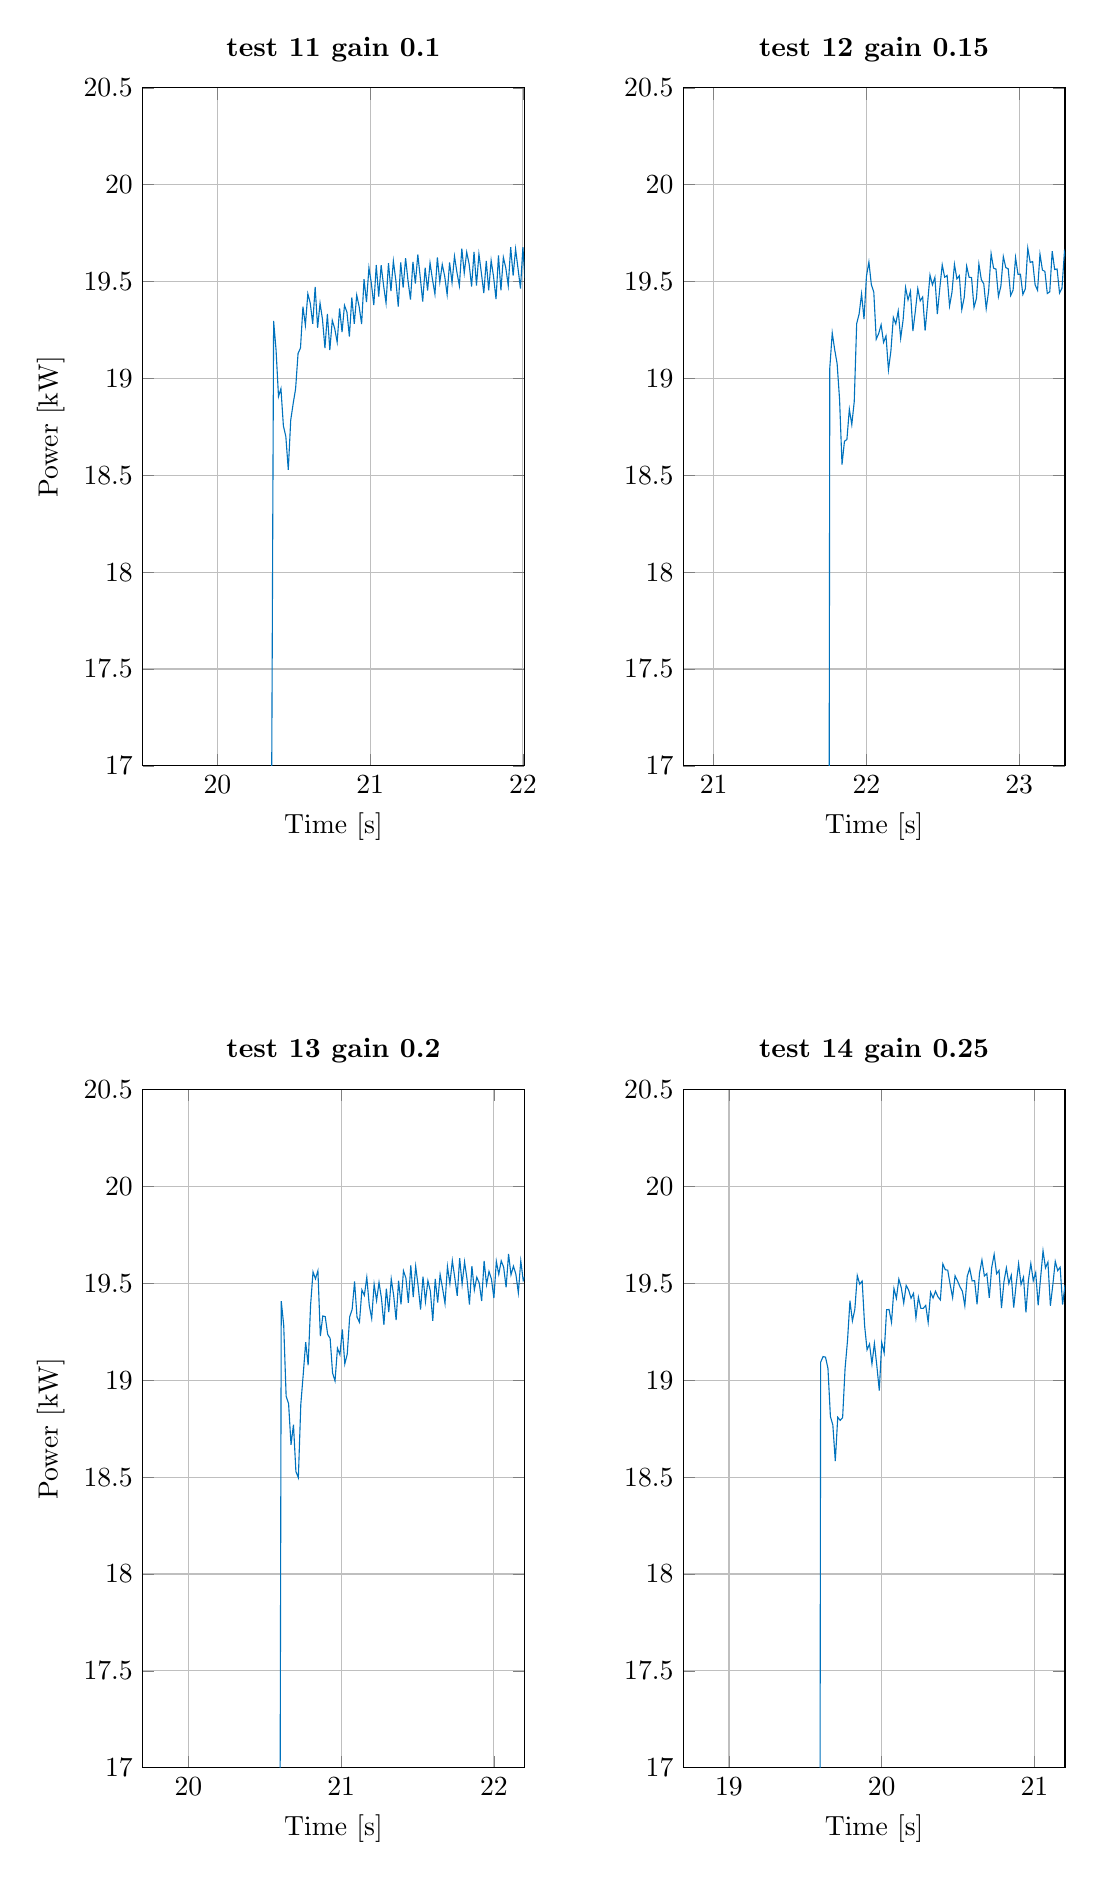
\begin{tikzpicture}

\begin{axis}[%
width=0.4\textwidth,
height=3.39in,
at={(1.297in,5.802in)},
scale only axis,
xmin=19.51,
xmax=22.01,
xlabel={Time [s]},
xmajorgrids,
ymin=17,
ymax=20.5,
ylabel={Power [kW]},
ymajorgrids,
axis background/.style={fill=white},
title style={font=\bfseries},
title={test 11 gain 0.1}
]
\addplot [color=mycolor1,solid,forget plot]
  table[row sep=crcr]{%
20.3539017595488	16.65\\
20.368	19.2971250831018\\
20.384	19.1471927015356\\
20.4	18.906455279542\\
20.416	18.947526581501\\
20.432	18.7552004196341\\
20.448	18.7002998998781\\
20.464	18.5287357201555\\
20.48	18.784753105439\\
20.496	18.8702189882239\\
20.512	18.9471719720944\\
20.528	19.1288474994648\\
20.544	19.1574958477805\\
20.56	19.3708905493402\\
20.576	19.2747267111773\\
20.592	19.437418906861\\
20.608	19.3881002751323\\
20.624	19.2818778957759\\
20.64	19.4722337626986\\
20.656	19.2618771027597\\
20.672	19.3887791646155\\
20.688	19.3046365023146\\
20.704	19.1561390701888\\
20.72	19.3327987594957\\
20.736	19.1462135645546\\
20.752	19.2997986197228\\
20.768	19.2573456026676\\
20.784	19.1875256887424\\
20.8	19.3612982398073\\
20.816	19.2388468852738\\
20.832	19.3773207998818\\
20.848	19.3424444521756\\
20.864	19.2158662146396\\
20.88	19.4176227339026\\
20.896	19.2813504515254\\
20.912	19.4302606362375\\
20.928	19.3705620764534\\
20.944	19.2808095969818\\
20.96	19.5122422487589\\
20.976	19.3937715214779\\
20.992	19.5716137704006\\
21.008	19.4898525142359\\
21.024	19.3787751162585\\
21.04	19.5854024710666\\
21.056	19.4227247136519\\
21.072	19.5847447096393\\
21.088	19.478698925621\\
21.104	19.3893845405218\\
21.12	19.5956856021556\\
21.136	19.4515792836436\\
21.152	19.606072443916\\
21.168	19.5068024833324\\
21.184	19.3706330091653\\
21.2	19.5988011128687\\
21.216	19.4685126866953\\
21.232	19.6210430205698\\
21.248	19.5030132720116\\
21.264	19.4066733344185\\
21.28	19.6018275008414\\
21.296	19.4902069298341\\
21.312	19.6395293791956\\
21.328	19.5215615456651\\
21.344	19.3963513403509\\
21.36	19.5711987581929\\
21.376	19.4538781829592\\
21.392	19.5964181527671\\
21.408	19.5107338149104\\
21.424	19.4349341487639\\
21.44	19.6247135508277\\
21.456	19.4968156475328\\
21.472	19.5883090147487\\
21.488	19.5273062913694\\
21.504	19.432995234104\\
21.52	19.5987906476708\\
21.536	19.4946458840511\\
21.552	19.6311261906458\\
21.568	19.5478239913088\\
21.584	19.4783503297671\\
21.6	19.6703497975857\\
21.616	19.5439912746775\\
21.632	19.6516728579774\\
21.648	19.5903764141055\\
21.664	19.4745894649401\\
21.68	19.6531228007305\\
21.696	19.4798908744253\\
21.712	19.6420322556479\\
21.728	19.5447189070381\\
21.744	19.4401789609729\\
21.76	19.6066340697492\\
21.776	19.455158422689\\
21.792	19.6091517284369\\
21.808	19.524389646839\\
21.824	19.4092760675648\\
21.84	19.6350197020537\\
21.856	19.4546473378267\\
21.872	19.6253850801925\\
21.888	19.5701383415472\\
21.904	19.4789283743988\\
21.92	19.6774898114179\\
21.936	19.5307491004891\\
21.952	19.6678502393407\\
21.968	19.5675158573074\\
21.984	19.4642206887475\\
22	19.6783259944804\\
22.016	19.4728283580646\\
};
\end{axis}

\begin{axis}[%
width=0.4\textwidth,
height=3.39in,
at={(4in,5.802in)},
scale only axis,
xmin=20.8,
xmax=23.3,
xlabel={Time [s]},
xmajorgrids,
ymin=17,
ymax=20.5,
ymajorgrids,
axis background/.style={fill=white},
title style={font=\bfseries},
title={test 12  gain 0.15}
]
\addplot [color=mycolor1,solid,forget plot]
  table[row sep=crcr]{%
21.7555204096517	16.65\\
21.76	19.0533899609115\\
21.776	19.2347331298192\\
21.792	19.1489582397232\\
21.808	19.076201693796\\
21.824	18.8916572786203\\
21.84	18.5557081066584\\
21.856	18.6758313636903\\
21.872	18.6846717089746\\
21.888	18.8409831878598\\
21.904	18.7618428532535\\
21.92	18.8799358927993\\
21.936	19.28277842158\\
21.952	19.332709496541\\
21.968	19.4368227215505\\
21.984	19.3061307994089\\
22	19.5279683623693\\
22.016	19.6011200365448\\
22.032	19.4840181142753\\
22.048	19.4454672689055\\
22.064	19.2027304083905\\
22.08	19.2317601346527\\
22.096	19.2770471542104\\
22.112	19.1859968343614\\
22.128	19.21936484066\\
22.144	19.0445054556632\\
22.16	19.1417326425094\\
22.176	19.3153180945766\\
22.192	19.2815585334627\\
22.208	19.3482937765136\\
22.224	19.2068871356952\\
22.24	19.3027075940535\\
22.256	19.4692082200941\\
22.272	19.4053440030875\\
22.288	19.4497871907807\\
22.304	19.2450633911372\\
22.32	19.3468547030673\\
22.336	19.4635985199093\\
22.352	19.400369736872\\
22.368	19.4204923636548\\
22.384	19.2465957488789\\
22.4	19.3854498833152\\
22.416	19.5336983828535\\
22.432	19.4830832646483\\
22.448	19.5217709635267\\
22.464	19.3323069428678\\
22.48	19.464626880179\\
22.496	19.5859199536123\\
22.512	19.5227089902865\\
22.528	19.5315398041826\\
22.544	19.3741487589766\\
22.56	19.4457828703788\\
22.576	19.589065191034\\
22.592	19.5140345708026\\
22.608	19.5302848910359\\
22.624	19.3552788067409\\
22.64	19.4179280369325\\
22.656	19.5799352505982\\
22.672	19.5225158090461\\
22.688	19.5207239952335\\
22.704	19.3666575880554\\
22.72	19.4133403509302\\
22.736	19.5908421669788\\
22.752	19.5099812783582\\
22.768	19.4881148476136\\
22.784	19.3603558330356\\
22.8	19.4518838765713\\
22.816	19.6439877282898\\
22.832	19.5695314836874\\
22.848	19.5642700965885\\
22.864	19.4226601516647\\
22.88	19.4765242539511\\
22.896	19.6292080301778\\
22.912	19.5725824511178\\
22.928	19.5657239388661\\
22.944	19.4280824259836\\
22.96	19.4559876975416\\
22.976	19.6239179253315\\
22.992	19.5377374527384\\
23.008	19.5376104607404\\
23.024	19.4332090903366\\
23.04	19.4627009071496\\
23.056	19.672519538106\\
23.072	19.5986641827951\\
23.088	19.6033243877019\\
23.104	19.4836040750878\\
23.12	19.4551973851599\\
23.136	19.6415663714753\\
23.152	19.5592949412008\\
23.168	19.5529733465587\\
23.184	19.4384574814443\\
23.2	19.4475051217176\\
23.216	19.657434651544\\
23.232	19.562816867934\\
23.248	19.5648777588739\\
23.264	19.4405640151427\\
23.28	19.4661103339828\\
23.296	19.6533160079817\\
23.312	19.6066447989189\\
};
\end{axis}

\begin{axis}[%
width=0.4\textwidth,
height=3.39in,
at={(1.297in,0.793in)},
scale only axis,
xmin=19.7,
xmax=22.2,
xlabel={Time [s]},
xmajorgrids,
ymin=17,
ymax=20.5,
ylabel={Power [kW]},
ymajorgrids,
axis background/.style={fill=white},
title style={font=\bfseries},
title={test 13  gain 0.2}
]
\addplot [color=mycolor1,solid,forget plot]
  table[row sep=crcr]{%
20.5999639001933	16.65\\
20.608	19.4086937094026\\
20.624	19.2861200207092\\
20.64	18.9169025867715\\
20.656	18.8794061344901\\
20.672	18.6670001042697\\
20.688	18.7707357777443\\
20.704	18.5280456109359\\
20.72	18.497006498008\\
20.736	18.875076982125\\
20.752	19.0316277365637\\
20.768	19.1966286821462\\
20.784	19.0775901223023\\
20.8	19.3871606354895\\
20.816	19.5592257143042\\
20.832	19.5237135574484\\
20.848	19.5651725269799\\
20.864	19.2275126893415\\
20.88	19.3319723370955\\
20.896	19.3277911479018\\
20.912	19.2368664611338\\
20.928	19.2160847126945\\
20.944	19.0370960715937\\
20.96	18.9964759942972\\
20.976	19.1651594245324\\
20.992	19.1320133065675\\
21.008	19.261918861108\\
21.024	19.0846399213941\\
21.04	19.1347115817299\\
21.056	19.3275669112387\\
21.072	19.364941728293\\
21.088	19.5098422713552\\
21.104	19.3259012691515\\
21.12	19.2991465431285\\
21.136	19.4662596821925\\
21.152	19.4382523265987\\
21.168	19.5314077782377\\
21.184	19.3871886815601\\
21.2	19.3188670515229\\
21.216	19.4954881811449\\
21.232	19.4113947163874\\
21.248	19.5049247488045\\
21.264	19.4233802602892\\
21.28	19.2860618206232\\
21.296	19.4730256182249\\
21.312	19.3514318342883\\
21.328	19.5231197219794\\
21.344	19.4371436598785\\
21.36	19.3102120463915\\
21.376	19.5133846624922\\
21.392	19.39143794059\\
21.408	19.5649075006589\\
21.424	19.52808201497\\
21.44	19.3990784663175\\
21.456	19.5932666475464\\
21.472	19.4292006354009\\
21.488	19.5881874696359\\
21.504	19.4872527479174\\
21.52	19.3652908535895\\
21.536	19.5344636297841\\
21.552	19.4058802001774\\
21.568	19.5135483909983\\
21.584	19.4604825306564\\
21.6	19.3063774912868\\
21.616	19.5234512093869\\
21.632	19.4004338754867\\
21.648	19.5459376206609\\
21.664	19.4747807774752\\
21.68	19.3959304079627\\
21.696	19.5869259365314\\
21.712	19.4984107688477\\
21.728	19.6176558101439\\
21.744	19.5288629097673\\
21.76	19.435668111695\\
21.776	19.630316964286\\
21.792	19.4950521566872\\
21.808	19.6111460570881\\
21.824	19.5220328979556\\
21.84	19.3908341802508\\
21.856	19.5894624703616\\
21.872	19.4659652910278\\
21.888	19.5320121337414\\
21.904	19.5014217207781\\
21.92	19.4093858744328\\
21.936	19.6156267405428\\
21.952	19.4936208815346\\
21.968	19.5620909995638\\
21.984	19.5224076609642\\
22	19.4236456934776\\
22.016	19.6136765374605\\
22.032	19.5467313175655\\
22.048	19.6165136099143\\
22.064	19.5833782356142\\
22.08	19.4792698903545\\
22.096	19.6519184821522\\
22.112	19.5442638677481\\
22.128	19.588831320272\\
22.144	19.5471364884538\\
22.16	19.4517707497502\\
22.176	19.616173769768\\
22.192	19.5151898192217\\
22.208	19.5454487253702\\
};
\end{axis}

\begin{axis}[%
width=0.4\textwidth,
height=3.39in,
at={(4in,0.793in)},
scale only axis,
xmin=18.7,
xmax=21.2,
xlabel={Time [s]},
xmajorgrids,
ymin=17,
ymax=20.5,
ymajorgrids,
axis background/.style={fill=white},
title style={font=\bfseries},
title={test 14  gain 0.25}
]
\addplot [color=mycolor1,solid,forget plot]
  table[row sep=crcr]{%
19.5958179987565	16.65\\
19.6	19.0927661655271\\
19.616	19.122313100031\\
19.632	19.1191211993489\\
19.648	19.0609738136073\\
19.664	18.8130627289322\\
19.68	18.7686273324438\\
19.696	18.5820939827833\\
19.712	18.8086668115843\\
19.728	18.7929570910272\\
19.744	18.8071414869708\\
19.76	19.0602019685105\\
19.776	19.2052159039639\\
19.792	19.4103520296618\\
19.808	19.3064020021676\\
19.824	19.3660299682837\\
19.84	19.5404576274496\\
19.856	19.4960291748992\\
19.872	19.5121904638652\\
19.888	19.2813508984953\\
19.904	19.1573709748084\\
19.92	19.1868475237973\\
19.936	19.0844887638524\\
19.952	19.1899733502434\\
19.968	19.0747638247155\\
19.984	18.9464595713765\\
20	19.1946245722861\\
20.016	19.1411181938764\\
20.032	19.3644295474144\\
20.048	19.3650962556655\\
20.064	19.2989167686081\\
20.08	19.4737875340213\\
20.096	19.4228499854925\\
20.112	19.5219879088825\\
20.128	19.4774091439638\\
20.144	19.3983165572681\\
20.16	19.4896812954271\\
20.176	19.465575425116\\
20.192	19.4231137791799\\
20.208	19.4484616041161\\
20.224	19.3225525250541\\
20.24	19.428856305941\\
20.256	19.3712198804158\\
20.272	19.3711537241465\\
20.288	19.3863280089857\\
20.304	19.2983788915309\\
20.32	19.4539383855806\\
20.336	19.4244900264941\\
20.352	19.4595198989554\\
20.368	19.4309551691469\\
20.384	19.4146756440096\\
20.4	19.6005569379725\\
20.416	19.570660901438\\
20.432	19.5682208236329\\
20.448	19.494067701179\\
20.464	19.4266139991146\\
20.48	19.5389678108614\\
20.496	19.5129118135001\\
20.512	19.4827883854189\\
20.528	19.4594777338079\\
20.544	19.384443229411\\
20.56	19.5381528571623\\
20.576	19.576956597249\\
20.592	19.5126944886236\\
20.608	19.5143552002601\\
20.624	19.3925051199014\\
20.64	19.5520129229583\\
20.656	19.6208243827026\\
20.672	19.5379363820899\\
20.688	19.5505555855172\\
20.704	19.4258909020477\\
20.72	19.5822623758526\\
20.736	19.6498574753558\\
20.752	19.5498460250129\\
20.768	19.5664897662641\\
20.784	19.3725326446509\\
20.8	19.5087251238893\\
20.816	19.5798488158452\\
20.832	19.4991356634641\\
20.848	19.5419188741309\\
20.864	19.3746387057234\\
20.88	19.4956978812876\\
20.896	19.6016979043382\\
20.912	19.4940747809488\\
20.928	19.5322592721585\\
20.944	19.3500782238377\\
20.96	19.5140240623719\\
20.976	19.6025731987395\\
20.992	19.5136556396136\\
21.008	19.5558065873397\\
21.024	19.3865014453996\\
21.04	19.528873105637\\
21.056	19.6680388205752\\
21.072	19.5804736489403\\
21.088	19.6098551001092\\
21.104	19.384752385106\\
21.12	19.4922071172538\\
21.136	19.6134351466772\\
21.152	19.565791075459\\
21.168	19.5835147064249\\
21.184	19.3906006620708\\
21.2	19.4911201313751\\
21.2	19.4911201313751\\
};
\end{axis}
\end{tikzpicture}%
\caption{Step from 10 to 20 kW load, with various scaling factors.}
\label{fig:test11-14-10to20kwsteppower}
\end{figure}

\begin{figure}[H]
\centering
% This file was created by matlab2tikz.
%
%The latest updates can be retrieved from
%  http://www.mathworks.com/matlabcentral/fileexchange/22022-matlab2tikz-matlab2tikz
%where you can also make suggestions and rate matlab2tikz.
%
\definecolor{mycolor1}{rgb}{0.00000,0.44700,0.74100}%
%
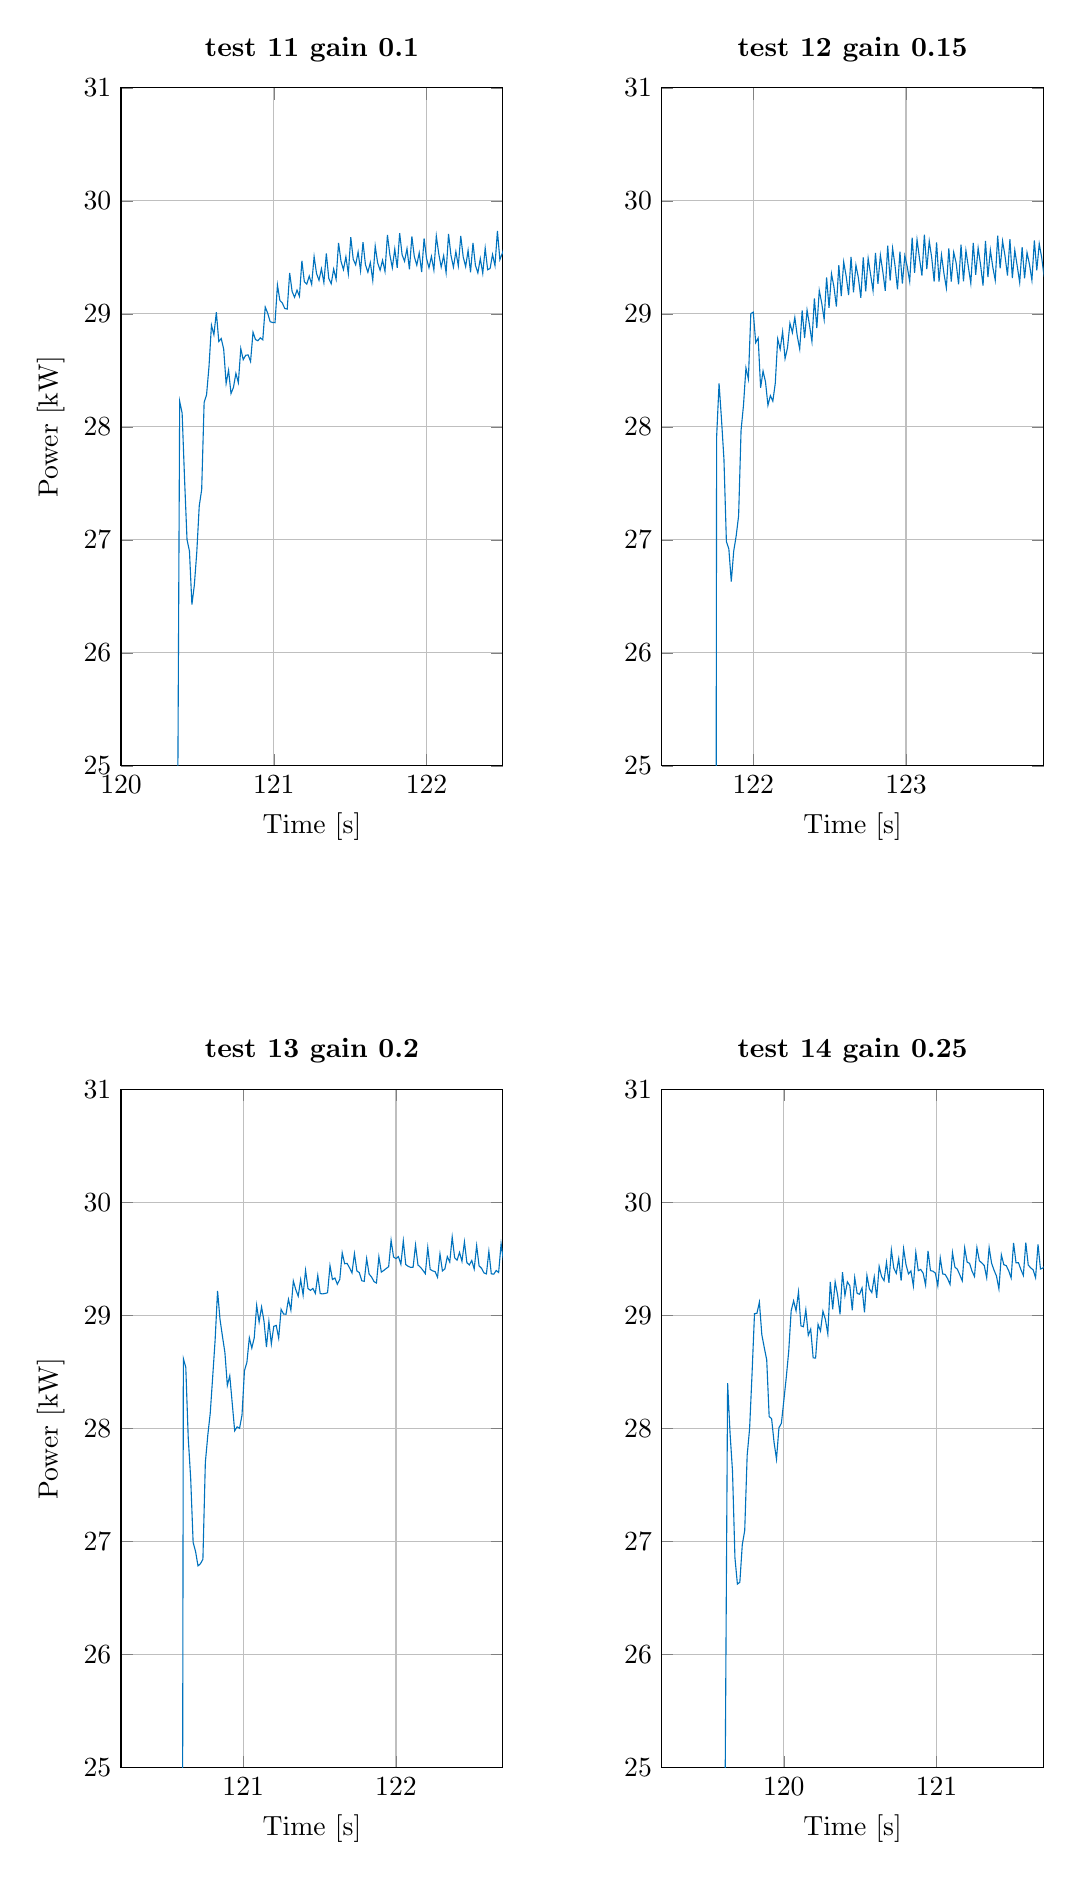
\begin{tikzpicture}

\begin{axis}[%
width=0.4\textwidth,
height=3.39in,
at={(1.297in,5.802in)},
scale only axis,
xmin=120,
xmax=122.5,
xlabel={Time [s]},
xmajorgrids,
ymin=25,
ymax=31,
ylabel={Power [kW]},
ymajorgrids,
axis background/.style={fill=white},
title style={font=\bfseries},
title={test 11 gain 0.1}
]
\addplot [color=mycolor1,solid,forget plot]
  table[row sep=crcr]{%
120.370209763586	24.4\\
120.384	28.2252433916687\\
120.4	28.1227227999483\\
120.416	27.5352415983054\\
120.432	27.0027026049854\\
120.448	26.9007292704487\\
120.464	26.4268844710763\\
120.48	26.6005872598819\\
120.496	26.8917623866278\\
120.512	27.2999588843677\\
120.528	27.4448937029763\\
120.544	28.2162115244312\\
120.56	28.2843696808009\\
120.576	28.5361336829596\\
120.592	28.8996460816284\\
120.608	28.8149722864846\\
120.624	29.0149038267143\\
120.64	28.7555179692389\\
120.656	28.7820460713145\\
120.672	28.6883163981257\\
120.688	28.3837764986913\\
120.704	28.501003134873\\
120.72	28.294891459891\\
120.736	28.3493638486745\\
120.752	28.473560255019\\
120.768	28.3911391967575\\
120.784	28.6919479645784\\
120.8	28.5947096049632\\
120.816	28.6332000070124\\
120.832	28.637065165209\\
120.848	28.5782084444307\\
120.864	28.8372747592683\\
120.88	28.7728334526805\\
120.896	28.7623592971841\\
120.912	28.7879423994889\\
120.928	28.7706692866643\\
120.944	29.0603389252388\\
120.96	29.0068672936651\\
120.976	28.9312677830774\\
120.992	28.9240484129301\\
121.008	28.9221462688349\\
121.024	29.2548562467405\\
121.04	29.1189736875932\\
121.056	29.0957004885948\\
121.072	29.0477229017507\\
121.088	29.0424596672691\\
121.104	29.3618989680058\\
121.12	29.1981298191361\\
121.136	29.1467970280152\\
121.152	29.210253200343\\
121.168	29.1554812823424\\
121.184	29.4696367494455\\
121.2	29.2854491715184\\
121.216	29.2633283404987\\
121.232	29.3342394348014\\
121.248	29.2614969815585\\
121.264	29.5070678640135\\
121.28	29.3565109819961\\
121.296	29.2971841283982\\
121.312	29.3990038736821\\
121.328	29.2768868202073\\
121.344	29.5345272142987\\
121.36	29.3140487948843\\
121.376	29.2663162368318\\
121.392	29.3960532661237\\
121.408	29.3068966865967\\
121.424	29.6277680872222\\
121.44	29.4652524247659\\
121.456	29.3915174890344\\
121.472	29.5047773019942\\
121.488	29.3552625508087\\
121.504	29.6794067908426\\
121.52	29.483907798732\\
121.536	29.4341177012706\\
121.552	29.5477535174118\\
121.568	29.3818061491094\\
121.584	29.6349466059824\\
121.6	29.4345346978718\\
121.616	29.3688612958011\\
121.632	29.4541613221275\\
121.648	29.2960048066704\\
121.664	29.5997588360975\\
121.68	29.4506795099818\\
121.696	29.3858036398005\\
121.712	29.4749763424817\\
121.728	29.37644838499\\
121.744	29.6991681009282\\
121.76	29.5218987285049\\
121.776	29.4080888990536\\
121.792	29.5740025052904\\
121.808	29.4080179810445\\
121.824	29.715187869538\\
121.84	29.5237202741134\\
121.856	29.4657772473196\\
121.872	29.5772270458098\\
121.888	29.394191225281\\
121.904	29.685682499572\\
121.92	29.506859617337\\
121.936	29.431207166736\\
121.952	29.540292773171\\
121.968	29.3697285740525\\
121.984	29.6673270943175\\
122	29.4900411231017\\
122.016	29.4081415611763\\
122.032	29.5083019570189\\
122.048	29.3878188137713\\
122.064	29.6893866890231\\
122.08	29.5317517309851\\
122.096	29.414045204535\\
122.112	29.5147239534048\\
122.128	29.364800982764\\
122.144	29.706772743324\\
122.16	29.5171925280896\\
122.176	29.4138740523356\\
122.192	29.5506420958164\\
122.208	29.4251669260417\\
122.224	29.6893221432526\\
122.24	29.5044452029501\\
122.256	29.418497501616\\
122.272	29.5614845870826\\
122.288	29.368001304985\\
122.304	29.6282042837452\\
122.32	29.429381380655\\
122.336	29.3626434092877\\
122.352	29.4897903550598\\
122.368	29.3593032684819\\
122.384	29.5820246686833\\
122.4	29.3904305343606\\
122.416	29.4012177615765\\
122.432	29.5250649684448\\
122.448	29.4273425584963\\
122.464	29.7341007336124\\
122.48	29.4801968403806\\
122.496	29.5348563742777\\
122.512	29.6101618569073\\
};
\end{axis}

\begin{axis}[%
width=0.4\textwidth,
height=3.39in,
at={(4in,5.802in)},
scale only axis,
xmin=121.4,
xmax=123.9,
xlabel={Time [s]},
xmajorgrids,
ymin=25,
ymax=31,
ymajorgrids,
axis background/.style={fill=white},
title style={font=\bfseries},
title={test 12  gain 0.15}
]
\addplot [color=mycolor1,solid,forget plot]
  table[row sep=crcr]{%
121.756717649747	24.4\\
121.76	27.9083335129483\\
121.776	28.3845430918921\\
121.792	28.0658599509874\\
121.808	27.7135643365179\\
121.824	26.984460679589\\
121.84	26.9212001201986\\
121.856	26.6314876884815\\
121.872	26.9013120916748\\
121.888	27.0345291287645\\
121.904	27.212841779221\\
121.92	27.9678242466907\\
121.936	28.1932906729235\\
121.952	28.522172446774\\
121.968	28.4234231277855\\
121.984	29.0028529577362\\
122	29.0151248227416\\
122.016	28.7448888446215\\
122.032	28.7863574355073\\
122.048	28.3461371404382\\
122.064	28.4941153361372\\
122.08	28.3985071561457\\
122.096	28.1912924953126\\
122.112	28.2763272846381\\
122.128	28.2273568096198\\
122.144	28.3854671784048\\
122.16	28.778337929305\\
122.176	28.6870782738458\\
122.192	28.8422557594243\\
122.208	28.6038244986242\\
122.224	28.6995768658719\\
122.24	28.9181100224273\\
122.256	28.8341962224993\\
122.272	28.968132188161\\
122.288	28.8031149734955\\
122.304	28.6886502343146\\
122.32	29.0303379825198\\
122.336	28.7866525802889\\
122.352	29.03317802342\\
122.368	28.9008373198097\\
122.384	28.7550046681927\\
122.4	29.1374912239336\\
122.416	28.8737861167187\\
122.432	29.2065942444395\\
122.448	29.0955489648155\\
122.464	28.9499491754765\\
122.48	29.322123178917\\
122.496	29.0527543732437\\
122.512	29.3544919924301\\
122.528	29.239490171754\\
122.544	29.0645664685719\\
122.56	29.4306852434514\\
122.576	29.1570672494854\\
122.592	29.4588745945372\\
122.608	29.3335760408194\\
122.624	29.167327849362\\
122.64	29.5048845427346\\
122.656	29.1913913058085\\
122.672	29.4309052476416\\
122.688	29.3197420139237\\
122.704	29.1419595614926\\
122.72	29.4999404771257\\
122.736	29.1985935754325\\
122.752	29.4911091521785\\
122.768	29.3478272582423\\
122.784	29.2049938521988\\
122.8	29.539702660905\\
122.816	29.2663040577577\\
122.832	29.5190980203975\\
122.848	29.3743587462556\\
122.864	29.2038056334224\\
122.88	29.6040918292748\\
122.896	29.2950036605198\\
122.912	29.5808784032117\\
122.928	29.4260162116965\\
122.944	29.2166186877309\\
122.96	29.5496497202903\\
122.976	29.2678947748014\\
122.992	29.5145712802603\\
123.008	29.4161111729437\\
123.024	29.2871506909761\\
123.04	29.6738680665753\\
123.056	29.3640301971095\\
123.072	29.6567449344617\\
123.088	29.4920594899088\\
123.104	29.3386524380031\\
123.12	29.7008033404625\\
123.136	29.395645260022\\
123.152	29.6440702401299\\
123.168	29.4980618317084\\
123.184	29.2867697129058\\
123.2	29.6318722219896\\
123.216	29.2855168837867\\
123.232	29.5217594398127\\
123.248	29.3599154304143\\
123.264	29.2292035500478\\
123.28	29.5782658473777\\
123.296	29.2855217180318\\
123.312	29.545018954419\\
123.328	29.4516649909336\\
123.344	29.2606474172281\\
123.36	29.6123295057329\\
123.376	29.2877204238451\\
123.392	29.5599021399745\\
123.408	29.4156218329584\\
123.424	29.270232606847\\
123.44	29.6284760231941\\
123.456	29.3465295394884\\
123.472	29.5825751480598\\
123.488	29.4327159466031\\
123.504	29.2506070550441\\
123.52	29.6455064991657\\
123.536	29.3257697680253\\
123.552	29.5639976161272\\
123.568	29.4133820846344\\
123.584	29.2975955409281\\
123.6	29.691884518702\\
123.616	29.4033707467014\\
123.632	29.6441785048651\\
123.648	29.5119538167358\\
123.664	29.3398327196356\\
123.68	29.6606403377171\\
123.696	29.3165403677421\\
123.712	29.5629783045596\\
123.728	29.4223273829955\\
123.744	29.2767699762029\\
123.76	29.5905259571902\\
123.776	29.3138051598637\\
123.792	29.5416774718931\\
123.808	29.4387970774334\\
123.824	29.2977774257826\\
123.84	29.649400729808\\
123.856	29.3862544922733\\
123.872	29.6200519163039\\
123.888	29.4986107025957\\
123.904	29.3258048979771\\
};
\end{axis}

\begin{axis}[%
width=0.4\textwidth,
height=3.39in,
at={(1.297in,0.793in)},
scale only axis,
xmin=120.2,
xmax=122.7,
xlabel={Time [s]},
xmajorgrids,
ymin=25,
ymax=31,
ylabel={Power [kW]},
ymajorgrids,
axis background/.style={fill=white},
title style={font=\bfseries},
title={test 13  gain 0.2}
]
\addplot [color=mycolor1,solid,forget plot]
  table[row sep=crcr]{%
120.602735884202	24.4\\
120.608	28.6204479784909\\
120.624	28.5423636433896\\
120.64	27.9181253374266\\
120.656	27.5607479360438\\
120.672	26.9940806140596\\
120.688	26.912839504326\\
120.704	26.7855677581543\\
120.72	26.8052054635872\\
120.736	26.8441399354557\\
120.752	27.7005364330111\\
120.768	27.9407429330598\\
120.784	28.1367809311473\\
120.8	28.4573719540583\\
120.816	28.7837250412733\\
120.832	29.2198975793186\\
120.848	28.9667864678935\\
120.864	28.8175419651089\\
120.88	28.6738678188079\\
120.896	28.3826792746807\\
120.912	28.4676234700264\\
120.928	28.2246012290964\\
120.944	27.9811712182897\\
120.96	28.0163409465986\\
120.976	28.0031760537593\\
120.992	28.1205269628491\\
121.008	28.5136406961106\\
121.024	28.5867476868887\\
121.04	28.8042434210961\\
121.056	28.7129771935292\\
121.072	28.8034127499314\\
121.088	29.0906848722377\\
121.104	28.9434588035739\\
121.12	29.0771795771687\\
121.136	28.9510300042774\\
121.152	28.721312903573\\
121.168	28.9483543258948\\
121.184	28.7495376301671\\
121.2	28.9056886521472\\
121.216	28.914101560744\\
121.232	28.8016794851047\\
121.248	29.0565511436426\\
121.264	29.0147752537062\\
121.28	29.012837687768\\
121.296	29.1455557422011\\
121.312	29.0491851203891\\
121.328	29.3068759744246\\
121.344	29.2307016699527\\
121.36	29.1722175759559\\
121.376	29.3196277726184\\
121.392	29.182494420583\\
121.408	29.4010900215883\\
121.424	29.2398493707786\\
121.44	29.2243011323947\\
121.456	29.2410871094236\\
121.472	29.1969788011611\\
121.488	29.3562662748631\\
121.504	29.1955668517105\\
121.52	29.1928664555104\\
121.536	29.1966816066105\\
121.552	29.2030932892908\\
121.568	29.4428647875776\\
121.584	29.3197792083793\\
121.6	29.3333243056838\\
121.616	29.2783225410515\\
121.632	29.3203747555141\\
121.648	29.5563654643181\\
121.664	29.4597110115751\\
121.68	29.4626357740375\\
121.696	29.4237458826393\\
121.712	29.378533405935\\
121.728	29.5495802311127\\
121.744	29.3956839891706\\
121.76	29.38088194985\\
121.776	29.3093713350703\\
121.792	29.3036092792706\\
121.808	29.5050110588732\\
121.824	29.3679988622459\\
121.84	29.3425152579761\\
121.856	29.3020547357233\\
121.872	29.2886439188646\\
121.888	29.5206395952535\\
121.904	29.3854086568128\\
121.92	29.4003516941721\\
121.936	29.4177689164415\\
121.952	29.4333700904185\\
121.968	29.6673622984477\\
121.984	29.519094275488\\
122	29.5046671588434\\
122.016	29.5228121142861\\
122.032	29.4545943234138\\
122.048	29.6625139358649\\
122.064	29.4523507785025\\
122.08	29.4365494634409\\
122.096	29.4273488267048\\
122.112	29.4290072626493\\
122.128	29.6248669980645\\
122.144	29.4484223041383\\
122.16	29.428817634178\\
122.176	29.4017624673935\\
122.192	29.3714867118378\\
122.208	29.603239132729\\
122.224	29.4095362048859\\
122.24	29.3964878124505\\
122.256	29.3898866362164\\
122.272	29.3397266540001\\
122.288	29.5472156330611\\
122.304	29.3961216563247\\
122.32	29.4137888100581\\
122.336	29.522481592432\\
122.352	29.474391977228\\
122.368	29.6969896196816\\
122.384	29.5126815785816\\
122.4	29.4912734693023\\
122.416	29.5603012450633\\
122.432	29.4804052645911\\
122.448	29.653566168672\\
122.464	29.4691927169365\\
122.48	29.4487288841615\\
122.496	29.4882887141649\\
122.512	29.413255424185\\
122.528	29.6202130753895\\
122.544	29.4405209602383\\
122.56	29.4194105558486\\
122.576	29.3783586071332\\
122.592	29.3697726585894\\
122.608	29.5695615007847\\
122.624	29.3699175539731\\
122.64	29.3672180753237\\
122.656	29.3998345901398\\
122.672	29.3821639197641\\
122.688	29.6365082855245\\
122.704	29.4803004735093\\
};
\end{axis}

\begin{axis}[%
width=0.4\textwidth,
height=3.39in,
at={(4in,0.793in)},
scale only axis,
xmin=119.2,
xmax=121.7,
xlabel={Time [s]},
xmajorgrids,
ymin=25,
ymax=31,
ymajorgrids,
axis background/.style={fill=white},
title style={font=\bfseries},
title={test 14  gain 0.25}
]
\addplot [color=mycolor1,solid,forget plot]
  table[row sep=crcr]{%
119.616	24.8836704868497\\
119.632	28.4031980988289\\
119.648	27.9594344381773\\
119.664	27.6245747695489\\
119.68	26.8580209449186\\
119.696	26.6247365442914\\
119.712	26.6409146036161\\
119.728	26.972003060545\\
119.744	27.1000454433598\\
119.76	27.7648025929372\\
119.776	28.0017111060939\\
119.792	28.4872792139893\\
119.808	29.0180120646274\\
119.824	29.0210491553711\\
119.84	29.1196406539856\\
119.856	28.8312685764573\\
119.872	28.7174155038957\\
119.888	28.6086374615949\\
119.904	28.10768749061\\
119.92	28.0886087702229\\
119.936	27.8796395264327\\
119.952	27.7301886480044\\
119.968	28.0081717938311\\
119.984	28.0476712619956\\
120	28.2487875226701\\
120.016	28.4539945376771\\
120.032	28.6844532966927\\
120.048	29.0424647343458\\
120.064	29.1312779131771\\
120.08	29.0431742308914\\
120.096	29.2102453246423\\
120.112	28.9098201670618\\
120.128	28.9022974428809\\
120.144	29.0530859191421\\
120.16	28.8262698556943\\
120.176	28.8812248796355\\
120.192	28.6265519858792\\
120.208	28.6248679953731\\
120.224	28.9233343592978\\
120.24	28.864074363512\\
120.256	29.0394382146204\\
120.272	28.9672929216228\\
120.288	28.8378612123036\\
120.304	29.2994186339052\\
120.32	29.0565356877144\\
120.336	29.2994614416088\\
120.352	29.1830571280597\\
120.368	29.0118118049929\\
120.384	29.3858566786149\\
120.4	29.1781983955848\\
120.416	29.2995609643446\\
120.432	29.2646982847721\\
120.448	29.0483604107593\\
120.464	29.3368470511356\\
120.48	29.1969830021497\\
120.496	29.1898525473008\\
120.512	29.2459094210097\\
120.528	29.0300088189182\\
120.544	29.3557011788947\\
120.56	29.2374899996265\\
120.576	29.2046189528456\\
120.592	29.3429008906211\\
120.608	29.1588538066731\\
120.624	29.4367286498339\\
120.64	29.3460592293963\\
120.656	29.3098937027835\\
120.672	29.4722943878294\\
120.688	29.2916454017085\\
120.704	29.5814819083459\\
120.72	29.4190294628401\\
120.736	29.3747337315309\\
120.752	29.502932403068\\
120.768	29.3098280804598\\
120.784	29.5927683441208\\
120.8	29.4504807546962\\
120.816	29.369997529344\\
120.832	29.3961165086311\\
120.848	29.2623815851993\\
120.864	29.5600164978674\\
120.88	29.3985453780785\\
120.896	29.4093360992512\\
120.912	29.3764035033712\\
120.928	29.2704102734187\\
120.944	29.5732926499893\\
120.96	29.3989207953476\\
120.976	29.3938246910919\\
120.992	29.3767622795115\\
121.008	29.2644667257217\\
121.024	29.5119133894847\\
121.04	29.3692857955955\\
121.056	29.3650195358284\\
121.072	29.3280634219445\\
121.088	29.2767578971604\\
121.104	29.5586607497821\\
121.12	29.4293744892117\\
121.136	29.4110958042441\\
121.152	29.3609836508354\\
121.168	29.3079086607986\\
121.184	29.5995430132765\\
121.2	29.4741188459185\\
121.216	29.4626914735493\\
121.232	29.3938937412436\\
121.248	29.3470047040904\\
121.264	29.6019419168233\\
121.28	29.4862044924015\\
121.296	29.4664566065678\\
121.312	29.4438271856516\\
121.328	29.336124687084\\
121.344	29.6026910159893\\
121.36	29.4643129709842\\
121.376	29.4027090164893\\
121.392	29.3508862776752\\
121.408	29.2369409944527\\
121.424	29.5390798427196\\
121.44	29.4511040188338\\
121.456	29.4423514565827\\
121.472	29.3974392177336\\
121.488	29.3343434784127\\
121.504	29.644313515036\\
121.52	29.4676565950958\\
121.536	29.4685117905421\\
121.552	29.4076899512433\\
121.568	29.3563226134369\\
121.584	29.6460000273297\\
121.6	29.4485699884758\\
121.616	29.4231308157175\\
121.632	29.4057799348581\\
121.648	29.336389507087\\
121.664	29.6302261717236\\
121.68	29.4129820133077\\
121.696	29.4219367788468\\
121.712	29.4478795708971\\
};
\end{axis}
\end{tikzpicture}%
\caption{Step from 10 to 30 kW load, with various scaling factors.}
\label{fig:test11-14-10to30kwsteppower}
\end{figure}

\begin{figure}[H]
\centering
% This file was created by matlab2tikz.
%
%The latest updates can be retrieved from
%  http://www.mathworks.com/matlabcentral/fileexchange/22022-matlab2tikz-matlab2tikz
%where you can also make suggestions and rate matlab2tikz.
%
\definecolor{mycolor1}{rgb}{0.00000,0.44700,0.74100}%
%
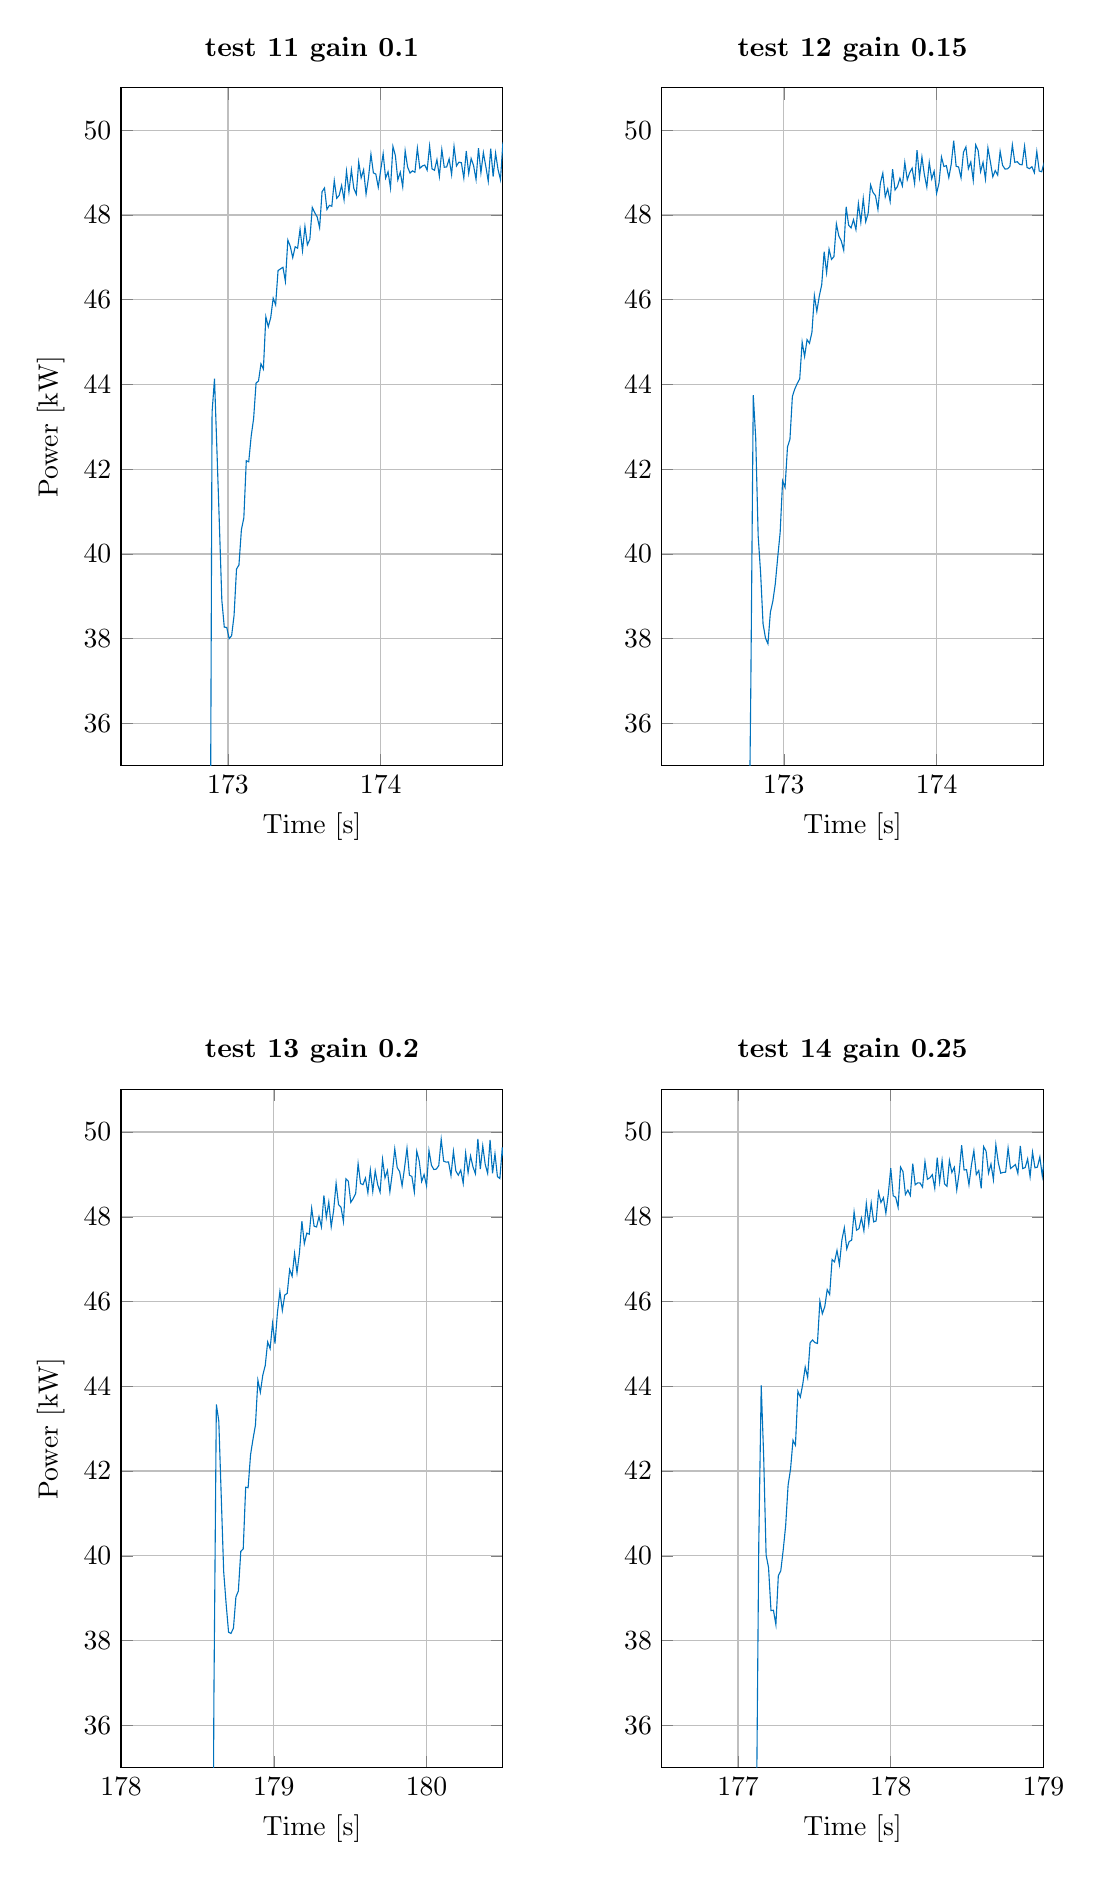
\begin{tikzpicture}

\begin{axis}[%
width=0.4\textwidth,
height=3.39in,
at={(1.297in,5.802in)},
scale only axis,
xmin=172.3,
xmax=174.8,
xlabel={Time [s]},
xmajorgrids,
ymin=35,
ymax=51,
ylabel={Power [kW]},
ymajorgrids,
axis background/.style={fill=white},
title style={font=\bfseries},
title={test 11 gain 0.1}
]
\addplot [color=mycolor1,solid,forget plot]
  table[row sep=crcr]{%
172.885469528002	33.4\\
172.896	43.3419459934948\\
172.912	44.1388116068426\\
172.928	42.4292758177869\\
172.944	40.6897657656201\\
172.96	38.9041729722595\\
172.976	38.2739198370799\\
172.992	38.2673855591398\\
173.008	38.0037169429951\\
173.024	38.0713943360174\\
173.04	38.5504737901647\\
173.056	39.6440451422691\\
173.072	39.7424296715405\\
173.088	40.5728213142966\\
173.104	40.8544219833913\\
173.12	42.2022890285361\\
173.136	42.1753536319374\\
173.152	42.7785334532434\\
173.168	43.1972425419949\\
173.184	44.0347942958678\\
173.2	44.0820822744443\\
173.216	44.4873169220332\\
173.232	44.3636017764039\\
173.248	45.5985544399626\\
173.264	45.3642494755149\\
173.28	45.5790564023115\\
173.296	46.0386435799344\\
173.312	45.879577204224\\
173.328	46.6886858119768\\
173.344	46.7293467818092\\
173.36	46.7656913086848\\
173.376	46.4339839858031\\
173.392	47.4087267515472\\
173.408	47.2599265898226\\
173.424	46.9938297173487\\
173.44	47.2496105781293\\
173.456	47.216204123017\\
173.472	47.6653602980574\\
173.488	47.1562174421746\\
173.504	47.7288955458638\\
173.52	47.2962762174881\\
173.536	47.4239871501946\\
173.552	48.1802180012667\\
173.568	48.0550777309629\\
173.584	47.954386721846\\
173.6	47.6997381826921\\
173.616	48.5493405377003\\
173.632	48.6380480356876\\
173.648	48.1311830456113\\
173.664	48.2277080120865\\
173.68	48.2059414835599\\
173.696	48.8103703318723\\
173.712	48.3927510059815\\
173.728	48.462584383723\\
173.744	48.6977182975709\\
173.76	48.3564748520089\\
173.776	49.0342971761523\\
173.792	48.5439576368181\\
173.808	49.066642073273\\
173.824	48.6269004484896\\
173.84	48.4894143296943\\
173.856	49.2481961355413\\
173.872	48.8750943200637\\
173.888	49.0668957046866\\
173.904	48.4909951430374\\
173.92	48.8822568761521\\
173.936	49.4364340189096\\
173.952	48.9938484502679\\
173.968	48.9649466565992\\
173.984	48.6543652116907\\
174	49.0626997077496\\
174.016	49.4469340581323\\
174.032	48.8704023544629\\
174.048	49.0203026570159\\
174.064	48.636850062461\\
174.08	49.61979572154\\
174.096	49.4006420945488\\
174.112	48.8285881162476\\
174.128	49.0099258747118\\
174.144	48.6659261971506\\
174.16	49.516346308174\\
174.176	49.1308028022296\\
174.192	48.9896095037051\\
174.208	49.0419819980367\\
174.224	49.0072118642753\\
174.24	49.576454800159\\
174.256	49.1006223462879\\
174.272	49.1555360661536\\
174.288	49.1782852812606\\
174.304	49.0589627419039\\
174.32	49.6313844131157\\
174.336	49.0881569725929\\
174.352	49.0556034643231\\
174.368	49.3071713845852\\
174.384	48.9097745913616\\
174.4	49.5443496213932\\
174.416	49.126559263978\\
174.432	49.1344173848726\\
174.448	49.3239308257022\\
174.464	48.9549513736362\\
174.48	49.6193839363069\\
174.496	49.1577822395667\\
174.512	49.2472163004269\\
174.528	49.2338986023726\\
174.544	48.8702497457535\\
174.56	49.5088879890602\\
174.576	48.9797549929778\\
174.592	49.3337560744145\\
174.608	49.1649595406493\\
174.624	48.8374799342085\\
174.64	49.5771220797861\\
174.656	48.9971769145509\\
174.672	49.4709375454491\\
174.688	49.1455548838565\\
174.704	48.7967296306133\\
174.72	49.56792383915\\
174.736	48.9059787672401\\
174.752	49.4604533645567\\
174.768	49.0748031510178\\
174.784	48.8336014311581\\
174.8	49.7144471316456\\
174.816	49.0129027437179\\
};
\end{axis}

\begin{axis}[%
width=0.4\textwidth,
height=3.39in,
at={(4in,5.802in)},
scale only axis,
xmin=172.2,
xmax=174.7,
xlabel={Time [s]},
xmajorgrids,
ymin=35,
ymax=51,
ymajorgrids,
axis background/.style={fill=white},
title style={font=\bfseries},
title={test 12  gain 0.15}
]
\addplot [color=mycolor1,solid,forget plot]
  table[row sep=crcr]{%
172.773848830464	33.4\\
172.784	36.9050562620521\\
172.8	43.7458800507488\\
172.816	42.7320845741707\\
172.832	40.4278514690103\\
172.848	39.5543864317928\\
172.864	38.3516486334802\\
172.88	38.0146833447863\\
172.896	37.880886150139\\
172.912	38.6268843816269\\
172.928	38.8843142068921\\
172.944	39.2938166385493\\
172.96	39.9229989554516\\
172.976	40.5105250420777\\
172.992	41.7263021677964\\
173.008	41.5712337991587\\
173.024	42.5269812147784\\
173.04	42.7072454538649\\
173.056	43.7200203845343\\
173.072	43.8950223195887\\
173.088	44.0252133972437\\
173.104	44.1328048880908\\
173.12	45.0009913131735\\
173.136	44.6603317008151\\
173.152	45.0583563065597\\
173.168	44.972958046498\\
173.184	45.2320786171303\\
173.2	46.0995421610033\\
173.216	45.7248648824918\\
173.232	46.0830285123882\\
173.248	46.3535531678859\\
173.264	47.1359395120575\\
173.28	46.6368536833937\\
173.296	47.1929323973756\\
173.312	46.9519924751873\\
173.328	47.0169134530714\\
173.344	47.7897638350725\\
173.36	47.5062477122113\\
173.376	47.3886899484094\\
173.392	47.1668237952704\\
173.408	48.1934770890665\\
173.424	47.7624383734178\\
173.44	47.694528350613\\
173.456	47.8890976063891\\
173.472	47.654983377399\\
173.488	48.271483179559\\
173.504	47.8284298639687\\
173.52	48.3898497712725\\
173.536	47.8417361032073\\
173.552	48.0397451843146\\
173.568	48.7092676659859\\
173.584	48.5320756202534\\
173.6	48.4567323711109\\
173.616	48.1306504023008\\
173.632	48.7530636043052\\
173.648	48.9870920720222\\
173.664	48.4278201588426\\
173.68	48.6179996461398\\
173.696	48.3192602514212\\
173.712	49.0816525241629\\
173.728	48.5902943825628\\
173.744	48.673119772192\\
173.76	48.8687252484111\\
173.776	48.6851273219454\\
173.792	49.2397131684759\\
173.808	48.8288589873109\\
173.824	49.0001214872108\\
173.84	49.1057407566989\\
173.856	48.7403829029922\\
173.872	49.5315531094434\\
173.888	48.8879669599905\\
173.904	49.3714919125101\\
173.92	48.9536352654196\\
173.936	48.6565143686005\\
173.952	49.2436007564273\\
173.968	48.8511869633384\\
173.984	49.0338711042534\\
174	48.510262824582\\
174.016	48.7557996366096\\
174.032	49.3682337590274\\
174.048	49.1443555295124\\
174.064	49.1632799601087\\
174.08	48.8819058159248\\
174.096	49.2010325658107\\
174.112	49.7511622097257\\
174.128	49.1492754764422\\
174.144	49.1330912490969\\
174.16	48.8770164969631\\
174.176	49.4830285195037\\
174.192	49.6071764537304\\
174.208	49.0914104748796\\
174.224	49.2523502216939\\
174.24	48.8183964157278\\
174.256	49.6558231454547\\
174.272	49.5225010964958\\
174.288	49.0223335816981\\
174.304	49.2429529754263\\
174.32	48.8460551449685\\
174.336	49.5847924752523\\
174.352	49.2583453435453\\
174.368	48.9016298204007\\
174.384	49.0477380071586\\
174.4	48.9414312890996\\
174.416	49.5020243262218\\
174.432	49.1712522567163\\
174.448	49.0841338713196\\
174.464	49.089329107734\\
174.48	49.145312749655\\
174.496	49.6552924257534\\
174.512	49.2421752388299\\
174.528	49.2574913367699\\
174.544	49.194239493867\\
174.56	49.183947687369\\
174.576	49.6254930811896\\
174.592	49.1223501022133\\
174.608	49.0941955388894\\
174.624	49.1389985401265\\
174.64	48.9979401054382\\
174.656	49.4986352892666\\
174.672	49.0397402285971\\
174.688	49.0194323639262\\
174.704	49.241539393361\\
};
\end{axis}

\begin{axis}[%
width=0.4\textwidth,
height=3.39in,
at={(1.297in,0.793in)},
scale only axis,
xmin=178,
xmax=180.5,
xlabel={Time [s]},
xmajorgrids,
ymin=35,
ymax=51,
ylabel={Power [kW]},
ymajorgrids,
axis background/.style={fill=white},
title style={font=\bfseries},
title={test 13  gain 0.2}
]
\addplot [color=mycolor1,solid,forget plot]
  table[row sep=crcr]{%
178.603563819994	33.4\\
178.608	36.6506229143476\\
178.624	43.5736066586891\\
178.64	43.1821777765106\\
178.656	41.4087490663681\\
178.672	39.6282412285775\\
178.688	38.8677637062828\\
178.704	38.1972888224683\\
178.72	38.1686328155515\\
178.736	38.2940200540573\\
178.752	39.0270201119462\\
178.768	39.1684943198641\\
178.784	40.1023121315378\\
178.8	40.1651369112139\\
178.816	41.6190361931452\\
178.832	41.6062506433582\\
178.848	42.3865295311999\\
178.864	42.7543173725372\\
178.88	43.0852441004745\\
178.896	44.1462235529426\\
178.912	43.8566505849212\\
178.928	44.2590795607483\\
178.944	44.489626103575\\
178.96	45.0470074933144\\
178.976	44.8893455992469\\
178.992	45.4844894962321\\
179.008	45.0091199491387\\
179.024	45.7416815510027\\
179.04	46.2358381872061\\
179.056	45.7897193740684\\
179.072	46.1543642165736\\
179.088	46.1936987285044\\
179.104	46.7567725224911\\
179.12	46.596062840153\\
179.136	47.1353386162567\\
179.152	46.6803747645626\\
179.168	47.1524641930956\\
179.184	47.8952831351748\\
179.2	47.3655870542997\\
179.216	47.6143501402447\\
179.232	47.5890196003938\\
179.248	48.2027923826989\\
179.264	47.7773508254883\\
179.28	47.7592287313919\\
179.296	48.0037063735678\\
179.312	47.7610845283974\\
179.328	48.5018703025667\\
179.344	47.9887840311217\\
179.36	48.3496552363164\\
179.376	47.7639422439496\\
179.392	48.1547948177341\\
179.408	48.7904586582794\\
179.424	48.28664233848\\
179.44	48.2242998340944\\
179.456	47.8884279931914\\
179.472	48.8961894247539\\
179.488	48.8388566596022\\
179.504	48.3407065939307\\
179.52	48.4311360595896\\
179.536	48.5489185028582\\
179.552	49.2528081462149\\
179.568	48.7846654279481\\
179.584	48.7577570191215\\
179.6	48.9142847179852\\
179.616	48.5649858088492\\
179.632	49.1060551264951\\
179.648	48.5974819429114\\
179.664	49.0820610500631\\
179.68	48.7624807436393\\
179.696	48.5822729731293\\
179.712	49.3576091272427\\
179.728	48.9183570105586\\
179.744	49.092120582729\\
179.76	48.5877964568491\\
179.776	49.0365419781629\\
179.792	49.6027501090761\\
179.808	49.1606228149477\\
179.824	49.0649916727014\\
179.84	48.7307190584388\\
179.856	49.1553516165192\\
179.872	49.6215849621378\\
179.888	48.9813448842809\\
179.904	48.9522025927904\\
179.92	48.5859345112024\\
179.936	49.5491626976518\\
179.952	49.3165396860116\\
179.968	48.8333330000729\\
179.984	48.995481672221\\
180	48.7323633227996\\
180.016	49.5655249175568\\
180.032	49.2174100160644\\
180.048	49.1151804124907\\
180.064	49.1249592320851\\
180.08	49.2093027863133\\
180.096	49.8322663197763\\
180.112	49.3137024042345\\
180.128	49.2910487244516\\
180.144	49.2927299560773\\
180.16	48.973023984536\\
180.176	49.5460237103143\\
180.192	49.0796382242283\\
180.208	48.9828500411407\\
180.224	49.1019285615196\\
180.24	48.7887790012086\\
180.256	49.5047382910864\\
180.272	49.0404803717362\\
180.288	49.4365318271051\\
180.304	49.17756461483\\
180.32	49.0155293266156\\
180.336	49.839121227787\\
180.352	49.1280157516756\\
180.368	49.6745095995158\\
180.384	49.2391243547567\\
180.4	49.0238074949661\\
180.416	49.8159299526067\\
180.432	49.0267901352008\\
180.448	49.4881998944849\\
180.464	48.9489561581672\\
180.48	48.9028237412783\\
180.496	49.6361786205661\\
180.512	49.1650378722294\\
};
\end{axis}

\begin{axis}[%
width=0.4\textwidth,
height=3.39in,
at={(4in,0.793in)},
scale only axis,
xmin=176.5,
xmax=179,
xlabel={Time [s]},
xmajorgrids,
ymin=35,
ymax=51,
ymajorgrids,
axis background/.style={fill=white},
title style={font=\bfseries},
title={test 14  gain 0.25}
]
\addplot [color=mycolor1,solid,forget plot]
  table[row sep=crcr]{%
177.12	33.4988874241968\\
177.136	40.2907817910985\\
177.152	44.0219098428585\\
177.168	42.3484456018963\\
177.184	40.0195259372089\\
177.2	39.7200807021736\\
177.216	38.7065390584591\\
177.232	38.7156947918311\\
177.248	38.3743517371463\\
177.264	39.5298605464614\\
177.28	39.6456751477715\\
177.296	40.1381999890774\\
177.312	40.7131580100202\\
177.328	41.6680174103972\\
177.344	42.0459640976055\\
177.36	42.7273709999894\\
177.376	42.6095873560417\\
177.392	43.8838387871083\\
177.408	43.7449226326074\\
177.424	44.0528858439701\\
177.44	44.4546414926622\\
177.456	44.2066823532625\\
177.472	45.0277729447517\\
177.488	45.0920555209133\\
177.504	45.0295331943546\\
177.52	45.0112280528976\\
177.536	46.00835618442\\
177.552	45.7127239527008\\
177.568	45.8772839649562\\
177.584	46.2838261431469\\
177.6	46.1656637721731\\
177.616	46.9944858344705\\
177.632	46.9361363019579\\
177.648	47.206296005981\\
177.664	46.8680855380512\\
177.68	47.4518179315129\\
177.696	47.7413614365239\\
177.712	47.2415014370811\\
177.728	47.4158591975393\\
177.744	47.4473924391571\\
177.76	48.1142440272409\\
177.776	47.6835182735104\\
177.792	47.720597598494\\
177.808	47.9699790326547\\
177.824	47.6691412689828\\
177.84	48.3125220450107\\
177.856	47.8267283608689\\
177.872	48.3240864421005\\
177.888	47.8803025735305\\
177.904	47.8998029731343\\
177.92	48.5768644485401\\
177.936	48.337033931808\\
177.952	48.4500134531913\\
177.968	48.0829438950251\\
177.984	48.5439369601172\\
178	49.1484279794933\\
178.016	48.4945839651891\\
178.032	48.4645888945053\\
178.048	48.2225890202069\\
178.064	49.1743515438124\\
178.08	49.0654545010332\\
178.096	48.5256232690886\\
178.112	48.6289454453644\\
178.128	48.5031905993019\\
178.144	49.2550731288472\\
178.16	48.7547176464853\\
178.176	48.8002857282507\\
178.192	48.7981901257726\\
178.208	48.6998628637164\\
178.224	49.2994950549813\\
178.24	48.8850486220467\\
178.256	48.9208454455517\\
178.272	48.9951300173057\\
178.288	48.6729124369477\\
178.304	49.3925275661934\\
178.32	48.8194637753713\\
178.336	49.3271487863318\\
178.352	48.7752009534274\\
178.368	48.7185477396557\\
178.384	49.3298397124879\\
178.4	49.0451094865527\\
178.416	49.1691747250166\\
178.432	48.6315832278999\\
178.448	49.0426474651001\\
178.464	49.6882659156809\\
178.48	49.1031076592803\\
178.496	49.1132122256767\\
178.512	48.752065993446\\
178.528	49.2177988817482\\
178.544	49.5600788692028\\
178.56	48.9945160855096\\
178.576	49.0924320628733\\
178.592	48.6710029735205\\
178.608	49.6561620928612\\
178.624	49.5482488738505\\
178.64	49.0301315817528\\
178.656	49.246964251049\\
178.672	48.8765253720901\\
178.688	49.7017483062143\\
178.704	49.2766866926518\\
178.72	49.0276792520807\\
178.736	49.0477039452592\\
178.752	49.0525472981153\\
178.768	49.6220717056256\\
178.784	49.1400122956485\\
178.8	49.1838496188798\\
178.816	49.2321672920809\\
178.832	49.0227278612775\\
178.848	49.6736332438213\\
178.864	49.1373078726114\\
178.88	49.1624491662095\\
178.896	49.3659215908954\\
178.912	48.9475360906368\\
178.928	49.5247544843458\\
178.944	49.1564975210334\\
178.96	49.1726688058139\\
178.976	49.4118524239641\\
178.992	48.9586330538574\\
179.008	49.4672411562586\\
};
\end{axis}
\end{tikzpicture}%
\caption{Step from 10 to 50 kW load, with various scaling factors.}
\label{fig:test11-14-10to50kwsteppower}
\end{figure}

\begin{figure}[H]
\centering
% This file was created by matlab2tikz.
%
%The latest updates can be retrieved from
%  http://www.mathworks.com/matlabcentral/fileexchange/22022-matlab2tikz-matlab2tikz
%where you can also make suggestions and rate matlab2tikz.
%
\definecolor{mycolor1}{rgb}{0.00000,0.44700,0.74100}%
%
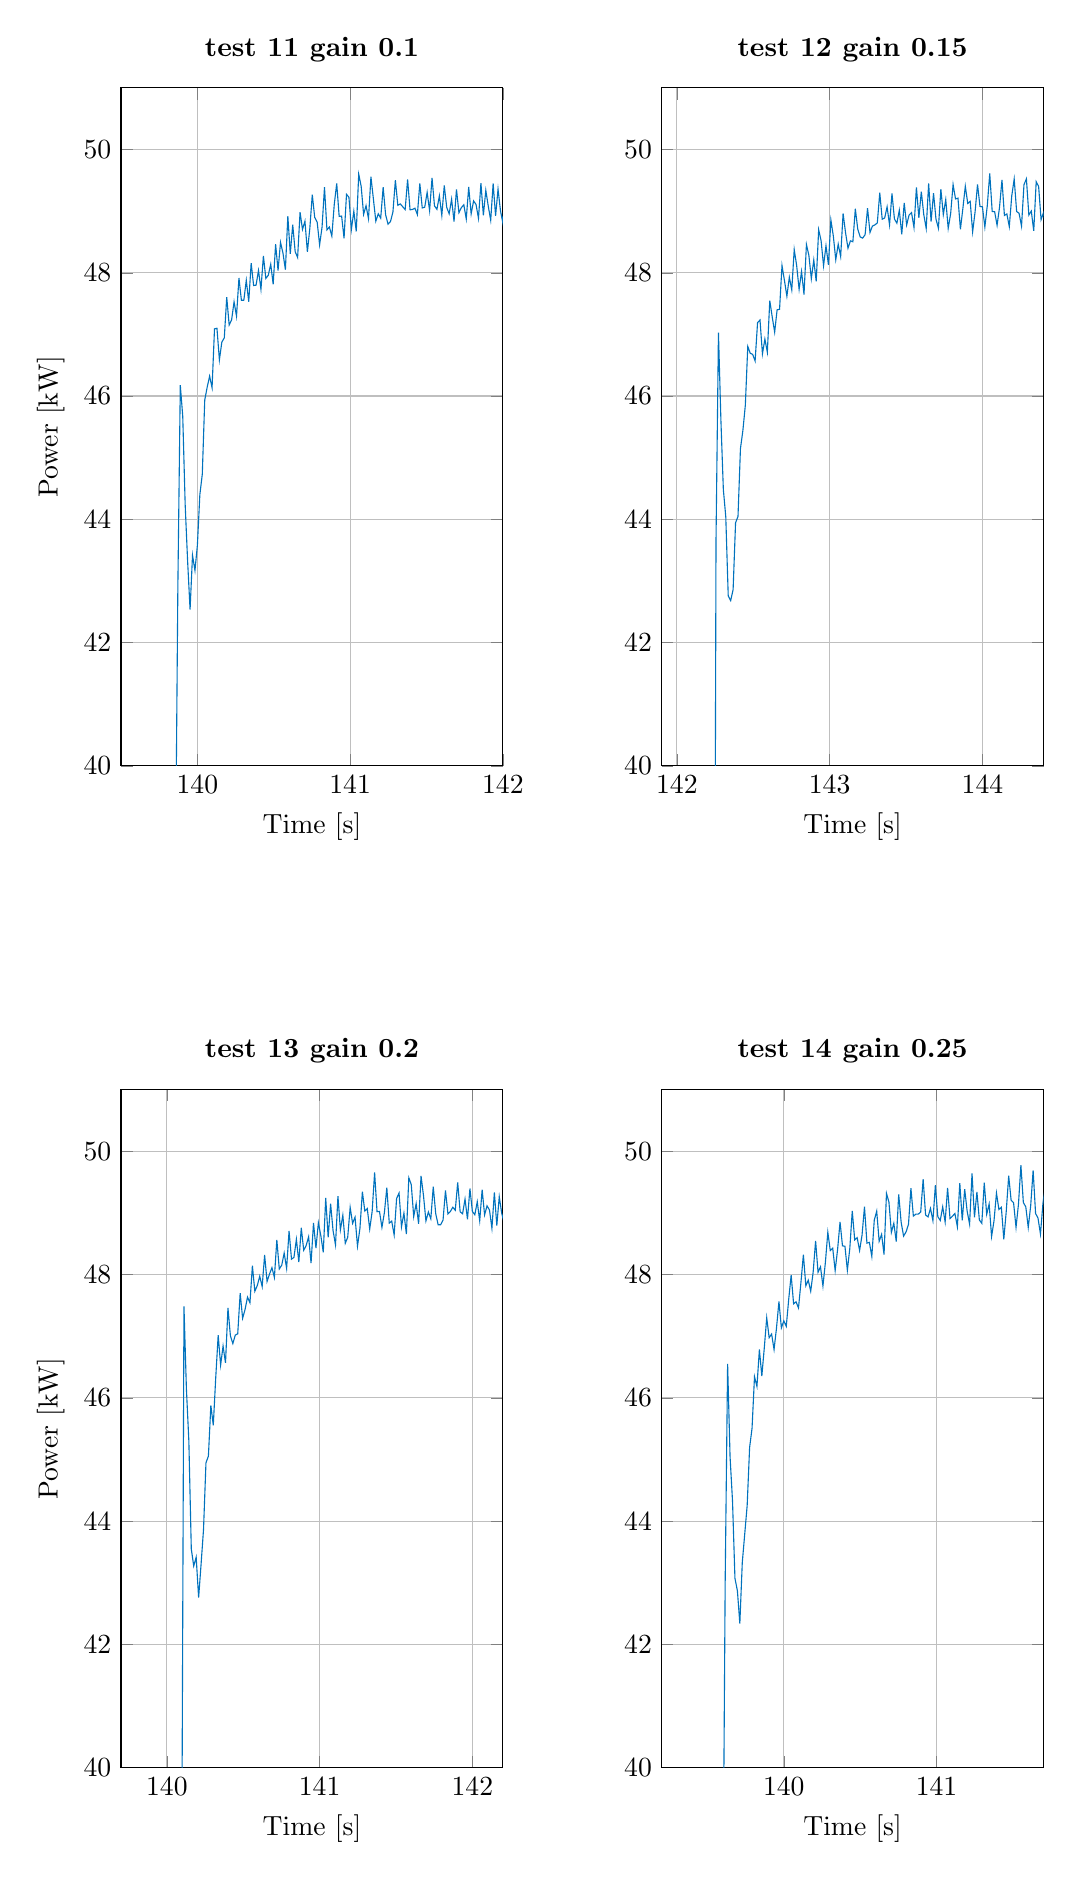
\begin{tikzpicture}

\begin{axis}[%
width=0.4\textwidth,
height=3.39in,
at={(1.297in,5.802in)},
scale only axis,
xmin=139.5,
xmax=142,
xlabel={Time [s]},
xmajorgrids,
ymin=40,
ymax=51,
ylabel={Power [kW]},
ymajorgrids,
axis background/.style={fill=white},
title style={font=\bfseries},
title={test 11 gain 0.1}
]
\addplot [color=mycolor1,solid,forget plot]
  table[row sep=crcr]{%
139.858605142475	38.9\\
139.872	42.8920371940288\\
139.888	46.1752156887972\\
139.904	45.6741573732266\\
139.92	44.2329950743606\\
139.936	43.3190074065711\\
139.952	42.5355103837549\\
139.968	43.4162272233854\\
139.984	43.1694100994534\\
140	43.5829964468035\\
140.016	44.3990141686011\\
140.032	44.7317508082235\\
140.048	45.9343494828896\\
140.064	46.1438335264947\\
140.08	46.3235837360232\\
140.096	46.1353531193308\\
140.112	47.0907652806933\\
140.128	47.0996952515252\\
140.144	46.5873759867906\\
140.16	46.8761231391991\\
140.176	46.9430452185528\\
140.192	47.602745666837\\
140.208	47.1524292649028\\
140.224	47.237042462999\\
140.24	47.5293395642667\\
140.256	47.2962216876352\\
140.272	47.9144842194001\\
140.288	47.5539872706055\\
140.304	47.5551672181577\\
140.32	47.8785198577072\\
140.336	47.5308062359744\\
140.352	48.1572949309711\\
140.368	47.7934038423925\\
140.384	47.7991462182263\\
140.4	48.0364177033493\\
140.416	47.7306435916911\\
140.432	48.2749250541779\\
140.448	47.9080695099134\\
140.464	47.9595512238793\\
140.48	48.1394960805151\\
140.496	47.8132280341813\\
140.512	48.463037202528\\
140.528	48.0367149408048\\
140.544	48.4929496770825\\
140.56	48.3219138266826\\
140.576	48.0499960431081\\
140.592	48.9201181196414\\
140.608	48.3079596776281\\
140.624	48.7810909389987\\
140.64	48.3423883523568\\
140.656	48.2486237267431\\
140.672	48.9820747159154\\
140.688	48.7037794512939\\
140.704	48.8367501474596\\
140.72	48.3394435440511\\
140.736	48.7219876172773\\
140.752	49.2679297161264\\
140.768	48.8974140048703\\
140.784	48.822568266838\\
140.8	48.4525051671345\\
140.816	48.7403734790411\\
140.832	49.3904976766086\\
140.848	48.6962732934032\\
140.864	48.7422371557232\\
140.88	48.5959009087737\\
140.896	49.1095998058526\\
140.912	49.4507414356977\\
140.928	48.9148682881611\\
140.944	48.9199673341155\\
140.96	48.5604650664398\\
140.976	49.2724669284223\\
140.992	49.2248210167115\\
141.008	48.7032601114972\\
141.024	48.9991691102913\\
141.04	48.6706409241904\\
141.056	49.6001894250528\\
141.072	49.4042200331369\\
141.088	48.9471651229157\\
141.104	49.0894944148193\\
141.12	48.8776817109433\\
141.136	49.5576228013781\\
141.152	49.1987569307632\\
141.168	48.8369761999923\\
141.184	48.9570041828391\\
141.2	48.8861675717711\\
141.216	49.3903766705684\\
141.232	48.9418279019142\\
141.248	48.78870220876\\
141.264	48.8318781091651\\
141.28	48.9856319139698\\
141.296	49.5033512804945\\
141.312	49.0943431259566\\
141.328	49.1174089962031\\
141.344	49.0717311962036\\
141.36	49.0251485792182\\
141.376	49.5140323451414\\
141.392	49.0213912529286\\
141.408	49.0281202596966\\
141.424	49.047970397072\\
141.44	48.9448531292728\\
141.456	49.4481490036907\\
141.472	49.0514561475524\\
141.488	49.0640603062343\\
141.504	49.304537091906\\
141.52	49.0077096629914\\
141.536	49.5395850079759\\
141.552	49.0845358634994\\
141.568	49.0292312295248\\
141.584	49.2491642525353\\
141.6	48.9287708910356\\
141.616	49.4167609081097\\
141.632	49.0618750026663\\
141.648	48.9570652144564\\
141.664	49.1955299878853\\
141.68	48.8317860826221\\
141.696	49.3536289043915\\
141.712	48.9749900491238\\
141.728	49.0564633861031\\
141.744	49.103713421258\\
141.76	48.8726895484538\\
141.776	49.3909721598601\\
141.792	48.9549194063945\\
141.808	49.1662252045215\\
141.824	49.1072315474743\\
141.84	48.8834867204626\\
141.856	49.4543564094769\\
141.872	48.9318479661827\\
141.888	49.3374845758219\\
141.904	49.0816012297072\\
141.92	48.8528212158998\\
141.936	49.4485833246964\\
141.952	48.9234910941172\\
141.968	49.3571498964875\\
141.984	49.0060487564628\\
142	48.8029985488856\\
142.016	49.5101478087092\\
};
\end{axis}

\begin{axis}[%
width=0.4\textwidth,
height=3.39in,
at={(4in,5.802in)},
scale only axis,
xmin=141.9,
xmax=144.4,
xlabel={Time [s]},
xmajorgrids,
ymin=40,
ymax=51,
ymajorgrids,
axis background/.style={fill=white},
title style={font=\bfseries},
title={test 12  gain 0.15}
]
\addplot [color=mycolor1,solid,forget plot]
  table[row sep=crcr]{%
142.250592451757	38.9\\
142.256	43.6475205736942\\
142.272	47.0302484023428\\
142.288	45.615824300486\\
142.304	44.4867528348838\\
142.32	44.0402441486984\\
142.336	42.7585656584966\\
142.352	42.681211006539\\
142.368	42.8602171414718\\
142.384	43.9433929798296\\
142.4	44.047568446208\\
142.416	45.1465189232784\\
142.432	45.4425626017716\\
142.448	45.850917972641\\
142.464	46.80572872628\\
142.48	46.6939253991157\\
142.496	46.6760199335467\\
142.512	46.5694496872496\\
142.528	47.1902536690378\\
142.544	47.2335363643562\\
142.56	46.6836226081334\\
142.576	46.9250877371424\\
142.592	46.7113646176459\\
142.608	47.547892301076\\
142.624	47.2832725719076\\
142.64	47.0355458054634\\
142.656	47.3998057165676\\
142.672	47.4073341150166\\
142.688	48.116834407212\\
142.704	47.8763929174111\\
142.72	47.6191922040313\\
142.736	47.9276899545488\\
142.752	47.721030194158\\
142.768	48.3765205110807\\
142.784	48.1165823740704\\
142.8	47.7318264946579\\
142.816	48.0220254011239\\
142.832	47.6476951870331\\
142.848	48.4584443318523\\
142.864	48.2822643962104\\
142.88	47.9038186343092\\
142.896	48.2079136775122\\
142.912	47.8595491894342\\
142.928	48.6978417080815\\
142.944	48.5194184332048\\
142.96	48.114485915109\\
142.976	48.4390456706167\\
142.992	48.1292053202341\\
143.008	48.8566478615002\\
143.024	48.5980186923899\\
143.04	48.2109390704286\\
143.056	48.4645627908104\\
143.072	48.2642447025717\\
143.088	48.9632826209575\\
143.104	48.6500304247936\\
143.12	48.3990038742709\\
143.136	48.5184272586679\\
143.152	48.503416602735\\
143.168	49.03801293655\\
143.184	48.7067012970763\\
143.2	48.581623057338\\
143.216	48.5628631896086\\
143.232	48.617204322972\\
143.248	49.0461851285098\\
143.264	48.6541590826939\\
143.28	48.7582001524013\\
143.296	48.7763240659657\\
143.312	48.8088083471302\\
143.328	49.2984088949798\\
143.344	48.8698133852545\\
143.36	48.8879171836837\\
143.376	49.0694270451782\\
143.392	48.7765204277407\\
143.408	49.2871334405764\\
143.424	48.873422158226\\
143.44	48.8041926573789\\
143.456	49.0142228548383\\
143.472	48.6229046748563\\
143.488	49.1345346374677\\
143.504	48.7764015038529\\
143.52	48.9380433224364\\
143.536	48.9761466004125\\
143.552	48.7344763060668\\
143.568	49.386408903207\\
143.584	48.891256899274\\
143.6	49.3168783630453\\
143.616	48.9458549672051\\
143.632	48.7193633051151\\
143.648	49.4494126623006\\
143.664	48.82937127636\\
143.68	49.2915416693321\\
143.696	48.8704951693126\\
143.712	48.723099111883\\
143.728	49.3575185865633\\
143.744	48.9437777825637\\
143.76	49.1880996111535\\
143.776	48.719685951353\\
143.792	48.9577407426696\\
143.808	49.4316756879834\\
143.824	49.1974095831899\\
143.84	49.211606352578\\
143.856	48.7055915867568\\
143.872	49.0427084709143\\
143.888	49.4038329601738\\
143.904	49.1246995505215\\
143.92	49.1593357215484\\
143.936	48.6637906460039\\
143.952	48.9885288458451\\
143.968	49.4338216586454\\
143.984	49.0769071442941\\
144	49.0709495334844\\
144.016	48.7417318519565\\
144.032	49.0914747257156\\
144.048	49.610420831082\\
144.064	48.9951781051406\\
144.08	48.9908874864776\\
144.096	48.770458855605\\
144.112	49.0618007098987\\
144.128	49.5068574914188\\
144.144	48.9305694576229\\
144.16	48.9540413669209\\
144.176	48.7487611858232\\
144.192	49.2468925413902\\
144.208	49.523017632145\\
144.224	48.9941150138597\\
144.24	48.9652682727959\\
144.256	48.7565216279484\\
144.272	49.4283561005739\\
144.288	49.5239820980691\\
144.304	48.9364602850693\\
144.32	49.0013536019475\\
144.336	48.6793184948335\\
144.352	49.4762532482556\\
144.368	49.4008061729342\\
144.384	48.8627106258082\\
144.4	48.9756562050707\\
144.416	48.5920176509648\\
};
\end{axis}

\begin{axis}[%
width=0.4\textwidth,
height=3.39in,
at={(1.297in,0.793in)},
scale only axis,
xmin=139.7,
xmax=142.2,
xlabel={Time [s]},
xmajorgrids,
ymin=40,
ymax=51,
ylabel={Power [kW]},
ymajorgrids,
axis background/.style={fill=white},
title style={font=\bfseries},
title={test 13  gain 0.2}
]
\addplot [color=mycolor1,solid,forget plot]
  table[row sep=crcr]{%
140.098392495046	38.9\\
140.112	47.4850763789135\\
140.128	46.1471751615921\\
140.144	45.3016613717805\\
140.16	43.5480625940269\\
140.176	43.2717637298568\\
140.192	43.414823170233\\
140.208	42.757979450411\\
140.224	43.2995425035822\\
140.24	43.8621849903594\\
140.256	44.9452067178269\\
140.272	45.0551464290641\\
140.288	45.8783008037945\\
140.304	45.5554502931647\\
140.32	46.3273084319016\\
140.336	47.0164071666755\\
140.352	46.5320469774061\\
140.368	46.8404920868282\\
140.384	46.566913931385\\
140.4	47.4584286856376\\
140.416	47.0064833540072\\
140.432	46.880627892105\\
140.448	47.0179661787284\\
140.464	47.0394103408568\\
140.48	47.700178979149\\
140.496	47.2901345277722\\
140.512	47.433599257268\\
140.528	47.6340799340838\\
140.544	47.5430049273899\\
140.56	48.1438011319117\\
140.576	47.7294775366809\\
140.592	47.8216713504769\\
140.608	47.9728420974066\\
140.624	47.8054967058983\\
140.64	48.3175728374945\\
140.656	47.8880604933024\\
140.672	48.0091631756228\\
140.688	48.1114406046393\\
140.704	47.954594697276\\
140.72	48.5630909275348\\
140.736	48.0907276441318\\
140.752	48.1522016242737\\
140.768	48.3490796150596\\
140.784	48.1007920047972\\
140.8	48.7075411048034\\
140.816	48.2500593561265\\
140.832	48.2790027045108\\
140.848	48.5719454462583\\
140.864	48.2021478327611\\
140.88	48.7589511345595\\
140.896	48.3941179265601\\
140.912	48.4722753568094\\
140.928	48.6134308908901\\
140.944	48.1847504329604\\
140.96	48.8371860042943\\
140.976	48.4311319805058\\
140.992	48.8416097375451\\
141.008	48.6305129399571\\
141.024	48.3619842744834\\
141.04	49.2431917479903\\
141.056	48.6035510221504\\
141.072	49.1493218799241\\
141.088	48.7144523215722\\
141.104	48.4817998946489\\
141.12	49.2730906286232\\
141.136	48.7261209225827\\
141.152	48.9636897854422\\
141.168	48.5074972777218\\
141.184	48.6056835962973\\
141.2	49.0901152389367\\
141.216	48.8308221162576\\
141.232	48.9308608470285\\
141.248	48.4619425005753\\
141.264	48.7494727480094\\
141.28	49.343239209399\\
141.296	49.0300737515184\\
141.312	49.0717381739117\\
141.328	48.7378395291769\\
141.344	49.0241672671836\\
141.36	49.6556185163873\\
141.376	49.0201690406263\\
141.392	49.0232468572145\\
141.408	48.7657124169816\\
141.424	49.0034124360019\\
141.44	49.4099519208385\\
141.456	48.8354953126885\\
141.472	48.8682658726502\\
141.488	48.6419696472288\\
141.504	49.2345935758342\\
141.52	49.322931816126\\
141.536	48.7746464197434\\
141.552	48.9976911423258\\
141.568	48.6566402711597\\
141.584	49.5700063478808\\
141.6	49.4605285930803\\
141.616	48.9410697102647\\
141.632	49.1512852426097\\
141.648	48.8247555835664\\
141.664	49.6002025988765\\
141.68	49.2827898441134\\
141.696	48.8706559014018\\
141.712	49.0152826083241\\
141.728	48.9056660613854\\
141.744	49.4269140421193\\
141.76	48.9888603338165\\
141.776	48.8078325955783\\
141.792	48.8078282135745\\
141.808	48.8833686785086\\
141.824	49.3634620439112\\
141.84	48.9851711701197\\
141.856	49.0245172900334\\
141.872	49.0924180032349\\
141.888	49.0429089709741\\
141.904	49.4951904290461\\
141.92	49.0188129014185\\
141.936	48.9866429361365\\
141.952	49.2244989456704\\
141.968	48.897112763023\\
141.984	49.3957676064293\\
142	49.0252551296499\\
142.016	48.9703767520487\\
142.032	49.1813976315582\\
142.048	48.871782252263\\
142.064	49.3783881609084\\
142.08	48.967685352849\\
142.096	49.1157386445423\\
142.112	49.0479307835695\\
142.128	48.7506360781094\\
142.144	49.3332727682852\\
142.16	48.795140640943\\
142.176	49.2623638008901\\
142.192	48.9972091663293\\
142.208	48.8361955138313\\
};
\end{axis}

\begin{axis}[%
width=0.4\textwidth,
height=3.39in,
at={(4in,0.793in)},
scale only axis,
xmin=139.2,
xmax=141.7,
xlabel={Time [s]},
xmajorgrids,
ymin=40,
ymax=51,
ymajorgrids,
axis background/.style={fill=white},
title style={font=\bfseries},
title={test 14  gain 0.25}
]
\addplot [color=mycolor1,solid,forget plot]
  table[row sep=crcr]{%
139.604825663627	38.9\\
139.616	42.9991613133902\\
139.632	46.5520630807243\\
139.648	45.0449728988374\\
139.664	44.3322655150933\\
139.68	43.0720697012203\\
139.696	42.8715648923326\\
139.712	42.337361207154\\
139.728	43.3269620705082\\
139.744	43.7899316675815\\
139.76	44.2542877703336\\
139.776	45.1944446732407\\
139.792	45.5085597608808\\
139.808	46.3452497315369\\
139.824	46.1874518028557\\
139.84	46.7842352131243\\
139.856	46.3537708187289\\
139.872	46.807885294345\\
139.888	47.298976693298\\
139.904	46.9763388404252\\
139.92	47.0350317032053\\
139.936	46.784116462722\\
139.952	47.132235653776\\
139.968	47.5628543828206\\
139.984	47.1353043214369\\
140	47.2494157985547\\
140.016	47.1600153315081\\
140.032	47.6007482066873\\
140.048	47.9918109767343\\
140.064	47.525489872375\\
140.08	47.5587334307669\\
140.096	47.4589103922057\\
140.112	47.8709521945063\\
140.128	48.3240374169053\\
140.144	47.818387914923\\
140.16	47.9092344539104\\
140.176	47.7295316684398\\
140.192	48.0391723409063\\
140.208	48.5468551023319\\
140.224	48.0375066365353\\
140.24	48.1256865232429\\
140.256	47.8143655365584\\
140.272	48.1958681930143\\
140.288	48.6870407796803\\
140.304	48.3908500963567\\
140.32	48.4293005997358\\
140.336	48.064203253759\\
140.352	48.4080319851642\\
140.368	48.8548008173355\\
140.384	48.4653230999715\\
140.4	48.4606461753948\\
140.416	48.0699908943212\\
140.432	48.4259074553266\\
140.448	49.0330396982073\\
140.464	48.5632978962555\\
140.48	48.5990906207355\\
140.496	48.3908370815541\\
140.512	48.6400389561132\\
140.528	49.1000906839277\\
140.544	48.5094649201931\\
140.56	48.5224100379568\\
140.576	48.2933457425207\\
140.592	48.8820374520252\\
140.608	49.0291684484761\\
140.624	48.5396743091723\\
140.64	48.6523095768671\\
140.656	48.3244487182258\\
140.672	49.3175593055188\\
140.688	49.1764780719829\\
140.704	48.683530858594\\
140.72	48.8326694348714\\
140.736	48.5349080392863\\
140.752	49.3023934857173\\
140.768	48.8489911713046\\
140.784	48.6238997014168\\
140.8	48.6920765527348\\
140.816	48.8126581473859\\
140.832	49.4002520845455\\
140.848	48.9491696312361\\
140.864	48.9797167644137\\
140.88	48.9797325283911\\
140.896	49.0144899440481\\
140.912	49.547656027015\\
140.928	48.9669671911754\\
140.944	48.9355695081398\\
140.96	49.0740873862399\\
140.976	48.8759147893705\\
140.992	49.4489894386515\\
141.008	48.941024010598\\
141.024	48.8778669769788\\
141.04	49.0991028314166\\
141.056	48.8518333287898\\
141.072	49.4063552986581\\
141.088	48.9077481106619\\
141.104	48.9482828429128\\
141.12	48.9914074769804\\
141.136	48.7761516185663\\
141.152	49.482787511368\\
141.168	48.8789356176275\\
141.184	49.3871012913641\\
141.2	49.0289669520958\\
141.216	48.8178294293218\\
141.232	49.6401426252783\\
141.248	48.9305331010843\\
141.264	49.339466048213\\
141.28	48.8859300778543\\
141.296	48.8318177455967\\
141.312	49.4895653838497\\
141.328	48.9777180301837\\
141.344	49.1457885777716\\
141.36	48.6184311912049\\
141.376	48.8756098326961\\
141.392	49.3219547069703\\
141.408	49.0558651002502\\
141.424	49.0926461943293\\
141.44	48.5725810639324\\
141.456	49.0258851096212\\
141.472	49.6035145424889\\
141.488	49.2045167225958\\
141.504	49.165227762298\\
141.52	48.7657783457445\\
141.536	49.1410192622509\\
141.552	49.7739824289417\\
141.568	49.1691620905236\\
141.584	49.0983064925177\\
141.6	48.7644992456435\\
141.616	49.1169158352107\\
141.632	49.6918353554049\\
141.648	48.9919876599711\\
141.664	48.9142554414164\\
141.68	48.6575986422701\\
141.696	49.1473898991479\\
141.712	49.4634995277867\\
};
\end{axis}
\end{tikzpicture}%
\caption{Step from 30 to 50 kW load, with various scaling factors.}
\label{fig:test11-14-30to50kwsteppower}
\end{figure}

\begin{figure}[H]
\centering
% This file was created by matlab2tikz.
%
%The latest updates can be retrieved from
%  http://www.mathworks.com/matlabcentral/fileexchange/22022-matlab2tikz-matlab2tikz
%where you can also make suggestions and rate matlab2tikz.
%
\definecolor{mycolor1}{rgb}{0.00000,0.44700,0.74100}%
%
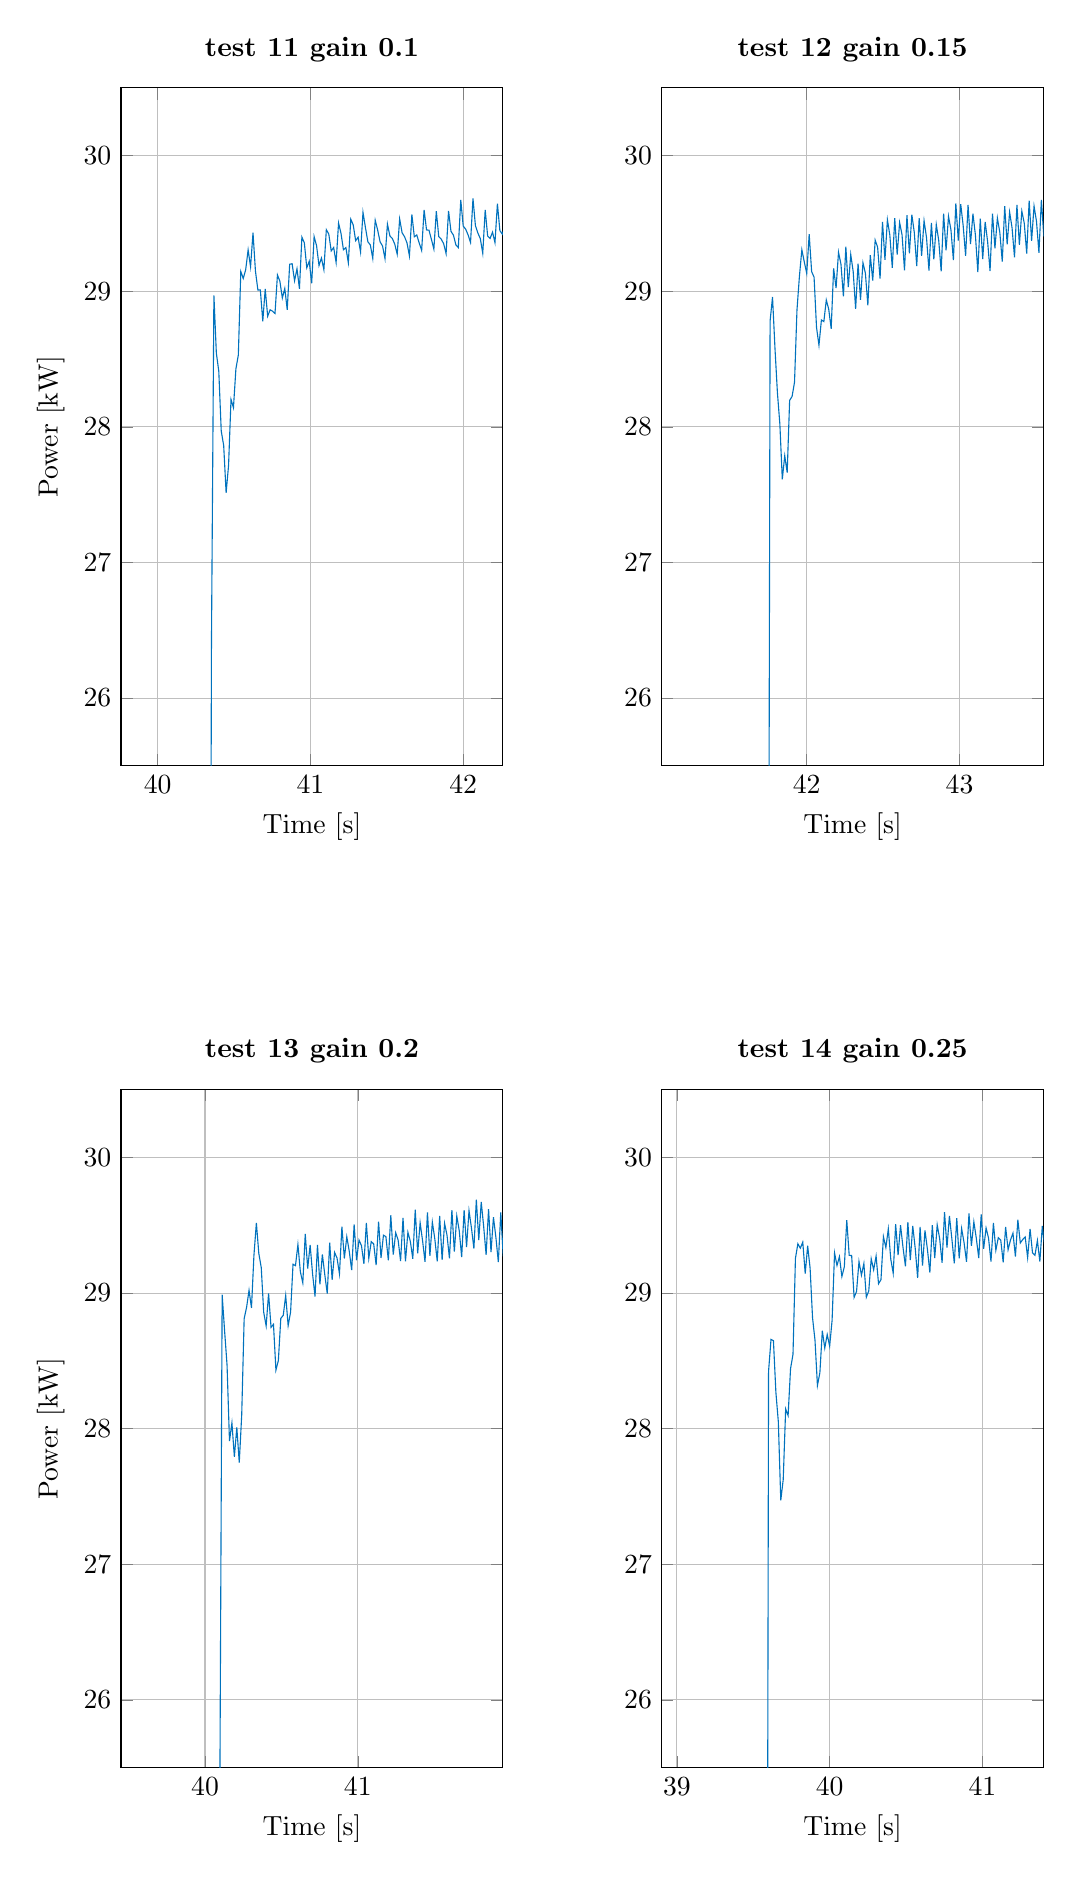
\begin{tikzpicture}

\begin{axis}[%
width=0.4\textwidth,
height=3.39in,
at={(1.297in,5.802in)},
scale only axis,
xmin=39.76,
xmax=42.26,
xlabel={Time [s]},
xmajorgrids,
ymin=25.5,
ymax=30.5,
ylabel={Power [kW]},
ymajorgrids,
axis background/.style={fill=white},
title style={font=\bfseries},
title={test 11 gain 0.1}
]
\addplot [color=mycolor1,solid,forget plot]
  table[row sep=crcr]{%
40.348762228564	25\\
40.352	26.3967812060208\\
40.368	28.9702524600522\\
40.384	28.5441906602587\\
40.4	28.4104082566813\\
40.416	27.9694073532004\\
40.432	27.8634766582351\\
40.448	27.5136498144581\\
40.464	27.7162620375186\\
40.48	28.2023170300644\\
40.496	28.141614267891\\
40.512	28.4274682620181\\
40.528	28.5302972675222\\
40.544	29.1458633159433\\
40.56	29.0944440699433\\
40.576	29.1582485598359\\
40.592	29.3053104290182\\
40.608	29.1806555100713\\
40.624	29.4321467400749\\
40.64	29.1484813101045\\
40.656	29.0090103706086\\
40.672	29.0102018714768\\
40.688	28.7790941409814\\
40.704	29.0164496902903\\
40.72	28.8157864457221\\
40.736	28.8633573305327\\
40.752	28.8532467758339\\
40.768	28.8362893936569\\
40.784	29.1206186376981\\
40.8	29.0736730461444\\
40.816	28.9496877345784\\
40.832	29.0209894156128\\
40.848	28.8634913586099\\
40.864	29.199243505866\\
40.88	29.2032586654278\\
40.896	29.0776119159898\\
40.912	29.1657106135391\\
40.928	29.018715141712\\
40.944	29.3991971752049\\
40.96	29.3576914607299\\
40.976	29.1731285688585\\
40.992	29.2213635040929\\
41.008	29.0581983476497\\
41.024	29.4032153963381\\
41.04	29.3365636201699\\
41.056	29.189953347786\\
41.072	29.2447993419298\\
41.088	29.1589753061008\\
41.104	29.4539751233132\\
41.12	29.4219927621057\\
41.136	29.2976641630543\\
41.152	29.3227990052339\\
41.168	29.2118694388458\\
41.184	29.5030931022786\\
41.2	29.4273321160782\\
41.216	29.3062178728077\\
41.232	29.3221036450499\\
41.248	29.2098392822724\\
41.264	29.5317551024444\\
41.28	29.4891203616968\\
41.296	29.3734316332445\\
41.312	29.3986344334656\\
41.328	29.2890995538899\\
41.344	29.5819769365933\\
41.36	29.4699074939795\\
41.376	29.3647648736481\\
41.392	29.3418631520482\\
41.408	29.2421243110184\\
41.424	29.5235208773816\\
41.44	29.4511340364688\\
41.456	29.3644272327438\\
41.472	29.3337529945923\\
41.488	29.2408494081089\\
41.504	29.4957292755088\\
41.52	29.408362478516\\
41.536	29.3897269923319\\
41.552	29.3472364463079\\
41.568	29.27322110745\\
41.584	29.5337720934785\\
41.6	29.4312938750137\\
41.616	29.4022748306667\\
41.632	29.3569883780693\\
41.648	29.2604939182631\\
41.664	29.5666317626308\\
41.68	29.4018391921866\\
41.696	29.4151764282551\\
41.712	29.355901577474\\
41.728	29.3008986283592\\
41.744	29.6004240068589\\
41.76	29.4523390819654\\
41.776	29.4502623947887\\
41.792	29.3823980878779\\
41.808	29.3107904269659\\
41.824	29.5900214708725\\
41.84	29.4026163914743\\
41.856	29.3847524381748\\
41.872	29.3509563218766\\
41.888	29.2776865986266\\
41.904	29.5932340301304\\
41.92	29.4420339625603\\
41.936	29.4143735604547\\
41.952	29.3421631602975\\
41.968	29.3222962066918\\
41.984	29.674533594879\\
42	29.4808211295406\\
42.016	29.4583331151358\\
42.032	29.4155595824374\\
42.048	29.3597272357884\\
42.064	29.6850835698728\\
42.08	29.4830622737175\\
42.096	29.4292888884519\\
42.112	29.3886666776748\\
42.128	29.2797800233787\\
42.144	29.6007819286797\\
42.16	29.4074779988213\\
42.176	29.389698398585\\
42.192	29.4358323234291\\
42.208	29.3585490050979\\
42.224	29.6465725148463\\
42.24	29.4476311333301\\
42.256	29.4214975295678\\
42.272	29.4759643355127\\
};
\end{axis}

\begin{axis}[%
width=0.4\textwidth,
height=3.39in,
at={(4in,5.802in)},
scale only axis,
xmin=41.05,
xmax=43.55,
xlabel={Time [s]},
xmajorgrids,
ymin=25.5,
ymax=30.5,
ymajorgrids,
axis background/.style={fill=white},
title style={font=\bfseries},
title={test 12  gain 0.15}
]
\addplot [color=mycolor1,solid,forget plot]
  table[row sep=crcr]{%
41.7526647874707	25\\
41.76	28.7799844290543\\
41.776	28.9574501128357\\
41.792	28.5802741998583\\
41.808	28.2519128444047\\
41.824	28.020660698688\\
41.84	27.6135818734054\\
41.856	27.7870278854862\\
41.872	27.6625629537304\\
41.888	28.195693166404\\
41.904	28.2241481485183\\
41.92	28.3291702205131\\
41.936	28.8607336414783\\
41.952	29.1096179664002\\
41.968	29.3062156314042\\
41.984	29.2156511833966\\
42	29.132124722964\\
42.016	29.4208824864754\\
42.032	29.1451908625921\\
42.048	29.1039740320268\\
42.064	28.7335653026807\\
42.08	28.6018440559262\\
42.096	28.7882477408264\\
42.112	28.7766325735689\\
42.128	28.9357255878741\\
42.144	28.8671070215895\\
42.16	28.7236130013419\\
42.176	29.1693443289174\\
42.192	29.0239722659121\\
42.208	29.2876909837447\\
42.224	29.1998064695468\\
42.24	28.961946219239\\
42.256	29.328307046027\\
42.272	29.0301857771139\\
42.288	29.271717630038\\
42.304	29.1454141581498\\
42.32	28.8697152546594\\
42.336	29.2039335481705\\
42.352	28.9370124315453\\
42.368	29.2105653879371\\
42.384	29.1330363756918\\
42.4	28.8966543321401\\
42.416	29.2671059166291\\
42.432	29.0788089201442\\
42.448	29.3774975148942\\
42.464	29.3242424731845\\
42.48	29.0939812832917\\
42.496	29.5117451408528\\
42.512	29.2315434317322\\
42.528	29.5276984392663\\
42.544	29.4134875131466\\
42.56	29.1723604399483\\
42.576	29.5387910681685\\
42.592	29.2711481352991\\
42.608	29.5072917389476\\
42.624	29.4154814287637\\
42.64	29.1551291594317\\
42.656	29.560429490178\\
42.672	29.2798430280273\\
42.688	29.5648838898466\\
42.704	29.433985419328\\
42.72	29.1861233427812\\
42.736	29.5388103386808\\
42.752	29.2614653947897\\
42.768	29.5200523161214\\
42.784	29.3970267154126\\
42.8	29.1533126201616\\
42.816	29.5036650989668\\
42.832	29.2354598944204\\
42.848	29.4923778128774\\
42.864	29.374773783311\\
42.88	29.1474669753292\\
42.896	29.5730057840228\\
42.912	29.3017613515356\\
42.928	29.5527505672336\\
42.944	29.4531424899451\\
42.96	29.2295110361727\\
42.976	29.6479810174381\\
42.992	29.3745936645671\\
43.008	29.6427484885756\\
43.024	29.4842115289432\\
43.04	29.2619691791025\\
43.056	29.6365508435134\\
43.072	29.3476048194136\\
43.088	29.572048661652\\
43.104	29.4159056719464\\
43.12	29.1421833201633\\
43.136	29.535203042912\\
43.152	29.2371974377152\\
43.168	29.5113326492034\\
43.184	29.3675061382929\\
43.2	29.1496909436654\\
43.216	29.5728571019306\\
43.232	29.3169922140402\\
43.248	29.5404366099469\\
43.264	29.432685467861\\
43.28	29.2184721398809\\
43.296	29.6282872641828\\
43.312	29.3453548176666\\
43.328	29.5837192291431\\
43.344	29.468589188367\\
43.36	29.2508153621887\\
43.376	29.6371580771595\\
43.392	29.342353613454\\
43.408	29.5909181201384\\
43.424	29.5017781804725\\
43.44	29.2781925213021\\
43.456	29.6683235835935\\
43.472	29.3722035995929\\
43.488	29.6282278829731\\
43.504	29.5152325451312\\
43.52	29.2842610822393\\
43.536	29.6742234749671\\
43.552	29.4034516082084\\
};
\end{axis}

\begin{axis}[%
width=0.4\textwidth,
height=3.39in,
at={(1.297in,0.793in)},
scale only axis,
xmin=39.45,
xmax=41.95,
xlabel={Time [s]},
xmajorgrids,
ymin=25.5,
ymax=30.5,
ylabel={Power [kW]},
ymajorgrids,
axis background/.style={fill=white},
title style={font=\bfseries},
title={test 13  gain 0.2}
]
\addplot [color=mycolor1,solid,forget plot]
  table[row sep=crcr]{%
40.096	25.0863856766849\\
40.112	28.9890920976219\\
40.128	28.7212137384488\\
40.144	28.4706627458571\\
40.16	27.9083379217708\\
40.176	28.0426747127097\\
40.192	27.7919018857829\\
40.208	28.010049690696\\
40.224	27.7493115822233\\
40.24	28.0992247490915\\
40.256	28.8112298376342\\
40.272	28.895358960096\\
40.288	29.0202566795543\\
40.304	28.8903423502471\\
40.32	29.2766928336705\\
40.336	29.5182248303587\\
40.352	29.2922000117317\\
40.368	29.1876942191824\\
40.384	28.8585451017014\\
40.4	28.7574558700109\\
40.416	28.9982796491136\\
40.432	28.7466874800687\\
40.448	28.7698045835578\\
40.464	28.4317219511996\\
40.48	28.5024831732086\\
40.496	28.8135808967526\\
40.512	28.8358623790003\\
40.528	28.982103043813\\
40.544	28.7596715588128\\
40.56	28.8593892725624\\
40.576	29.212913703145\\
40.592	29.202498463864\\
40.608	29.3576669171767\\
40.624	29.1568770530891\\
40.64	29.0753991011747\\
40.656	29.4358235676567\\
40.672	29.1809830257838\\
40.688	29.3552754552942\\
40.704	29.1401776436606\\
40.72	28.9749784574501\\
40.736	29.3559395620015\\
40.752	29.0635864898777\\
40.768	29.285678769776\\
40.784	29.1349906186022\\
40.8	28.9956695963777\\
40.816	29.3718165359574\\
40.832	29.0983607525239\\
40.848	29.2996259349331\\
40.864	29.2584386643689\\
40.88	29.1417517990415\\
40.896	29.4902620350482\\
40.912	29.2553228337832\\
40.928	29.4155902347093\\
40.944	29.3085890665975\\
40.96	29.1688702467553\\
40.976	29.5059349014728\\
40.992	29.2423746438382\\
41.008	29.3910019904004\\
41.024	29.3496193315323\\
41.04	29.2159286421514\\
41.056	29.5167385801859\\
41.072	29.2554677135387\\
41.088	29.3795158333619\\
41.104	29.3626902633522\\
41.12	29.2064630925\\
41.136	29.5261720743047\\
41.152	29.2590448205355\\
41.168	29.4268499737288\\
41.184	29.4161594750503\\
41.2	29.2406467154278\\
41.216	29.5736600110188\\
41.232	29.2838460215213\\
41.248	29.4458379915027\\
41.264	29.3911875402357\\
41.28	29.2366423850835\\
41.296	29.5538538470213\\
41.312	29.2347982247081\\
41.328	29.4486926244183\\
41.344	29.3807683440177\\
41.36	29.2530532199657\\
41.376	29.6142480330465\\
41.392	29.2931826039698\\
41.408	29.5185034182229\\
41.424	29.3870022745014\\
41.44	29.2300331654048\\
41.456	29.5956958810735\\
41.472	29.2743147950162\\
41.488	29.5230646674669\\
41.504	29.401080853915\\
41.52	29.2334902271361\\
41.536	29.5683049826788\\
41.552	29.2443965495258\\
41.568	29.5142767447347\\
41.584	29.4271640283303\\
41.6	29.2554720738224\\
41.616	29.6123304150294\\
41.632	29.3050590275519\\
41.648	29.5685683633102\\
41.664	29.4608839285752\\
41.68	29.2652839992468\\
41.696	29.6116656191471\\
41.712	29.3399687754483\\
41.728	29.6079831083344\\
41.744	29.4800818106923\\
41.76	29.3285705156563\\
41.776	29.6888545201814\\
41.792	29.39126769647\\
41.808	29.6720351082726\\
41.824	29.4909855782254\\
41.84	29.2819910093106\\
41.856	29.6195442082063\\
41.872	29.3013663833212\\
41.888	29.5590253517879\\
41.904	29.4114421947953\\
41.92	29.2278615391179\\
41.936	29.5942030172647\\
41.952	29.2704558032348\\
};
\end{axis}

\begin{axis}[%
width=0.4\textwidth,
height=3.39in,
at={(4in,0.793in)},
scale only axis,
xmin=38.9,
xmax=41.4,
xlabel={Time [s]},
xmajorgrids,
ymin=25.5,
ymax=30.5,
ymajorgrids,
axis background/.style={fill=white},
title style={font=\bfseries},
title={test 14  gain 0.25}
]
\addplot [color=mycolor1,solid,forget plot]
  table[row sep=crcr]{%
39.5937906584629	25\\
39.6	28.421704705968\\
39.616	28.657982073582\\
39.632	28.6487169782666\\
39.648	28.2682687683479\\
39.664	28.0508060138355\\
39.68	27.4708910766198\\
39.696	27.6243073859145\\
39.712	28.1451024715576\\
39.728	28.0969245850755\\
39.744	28.4427845548093\\
39.76	28.5477156703546\\
39.776	29.2566307746421\\
39.792	29.3634354815707\\
39.808	29.3310121032457\\
39.824	29.3754453695233\\
39.84	29.1433452749337\\
39.856	29.3486151980645\\
39.872	29.183332574223\\
39.888	28.8171044746461\\
39.904	28.6531468344631\\
39.92	28.3181957582216\\
39.936	28.4127096391141\\
39.952	28.721981666238\\
39.968	28.5940178106771\\
39.984	28.6942620351803\\
40	28.6085589491395\\
40.016	28.7996051234418\\
40.032	29.2957220318276\\
40.048	29.2033074083579\\
40.064	29.2686403353948\\
40.08	29.1221150222981\\
40.096	29.1930520148768\\
40.112	29.5374145599931\\
40.128	29.2775539798737\\
40.144	29.2772286823886\\
40.16	28.9682093747602\\
40.176	29.0117625045629\\
40.192	29.2325941755845\\
40.208	29.1320855730293\\
40.224	29.2183788078632\\
40.24	28.969501863639\\
40.256	29.01578330962\\
40.272	29.2529593879125\\
40.288	29.1717947615742\\
40.304	29.2728423714798\\
40.32	29.068513762939\\
40.336	29.0992474217305\\
40.352	29.4160896412188\\
40.368	29.335753499374\\
40.384	29.4735936396375\\
40.4	29.2510883453206\\
40.416	29.1460609257442\\
40.432	29.5078086514114\\
40.448	29.2804031828801\\
40.464	29.5005857963381\\
40.48	29.3385754034853\\
40.496	29.1974311554259\\
40.512	29.5235951101584\\
40.528	29.2429405924882\\
40.544	29.4952427642009\\
40.56	29.3312322072793\\
40.576	29.1114698309695\\
40.592	29.4875105150701\\
40.608	29.2031045280956\\
40.624	29.4621424559676\\
40.64	29.3226618533258\\
40.656	29.1514161463652\\
40.672	29.5010110093082\\
40.688	29.2585433602892\\
40.704	29.5029986445823\\
40.72	29.4024507633091\\
40.736	29.2234087425358\\
40.752	29.5966478075687\\
40.768	29.3354753286314\\
40.784	29.5686054368556\\
40.8	29.4006696012728\\
40.816	29.2186704294306\\
40.832	29.552842787551\\
40.848	29.2562867178971\\
40.864	29.4753560843516\\
40.88	29.3703432374439\\
40.896	29.2303560452229\\
40.912	29.5871095948556\\
40.928	29.3487591930865\\
40.944	29.5250590196483\\
40.96	29.4044463674877\\
40.976	29.2583137019548\\
40.992	29.5795006362031\\
41.008	29.3261517432604\\
41.024	29.480187681645\\
41.04	29.4057717963141\\
41.056	29.2320962298309\\
41.072	29.5171236003173\\
41.088	29.3159030474189\\
41.104	29.4087129328507\\
41.12	29.3906362779678\\
41.136	29.2268098707677\\
41.152	29.4877996149995\\
41.168	29.3197229603294\\
41.184	29.3921463888139\\
41.2	29.4417163964671\\
41.216	29.2693513234009\\
41.232	29.5408946564231\\
41.248	29.3693959571941\\
41.264	29.3949910877108\\
41.28	29.4142436748408\\
41.296	29.2619230094807\\
41.312	29.4736507214805\\
41.328	29.2961604008428\\
41.344	29.2785013089125\\
41.36	29.3872860334717\\
41.376	29.2326085621552\\
41.392	29.495054097524\\
41.408	29.3324412784058\\
};
\end{axis}
\end{tikzpicture}%
\caption{Step from 20 to 30 kW load, with various scaling factors.}
\label{fig:test11-14-20to30kwsteppower}
\end{figure}

\begin{figure}[H]
\centering
% This file was created by matlab2tikz.
%
%The latest updates can be retrieved from
%  http://www.mathworks.com/matlabcentral/fileexchange/22022-matlab2tikz-matlab2tikz
%where you can also make suggestions and rate matlab2tikz.
%
\definecolor{mycolor1}{rgb}{0.00000,0.44700,0.74100}%
%
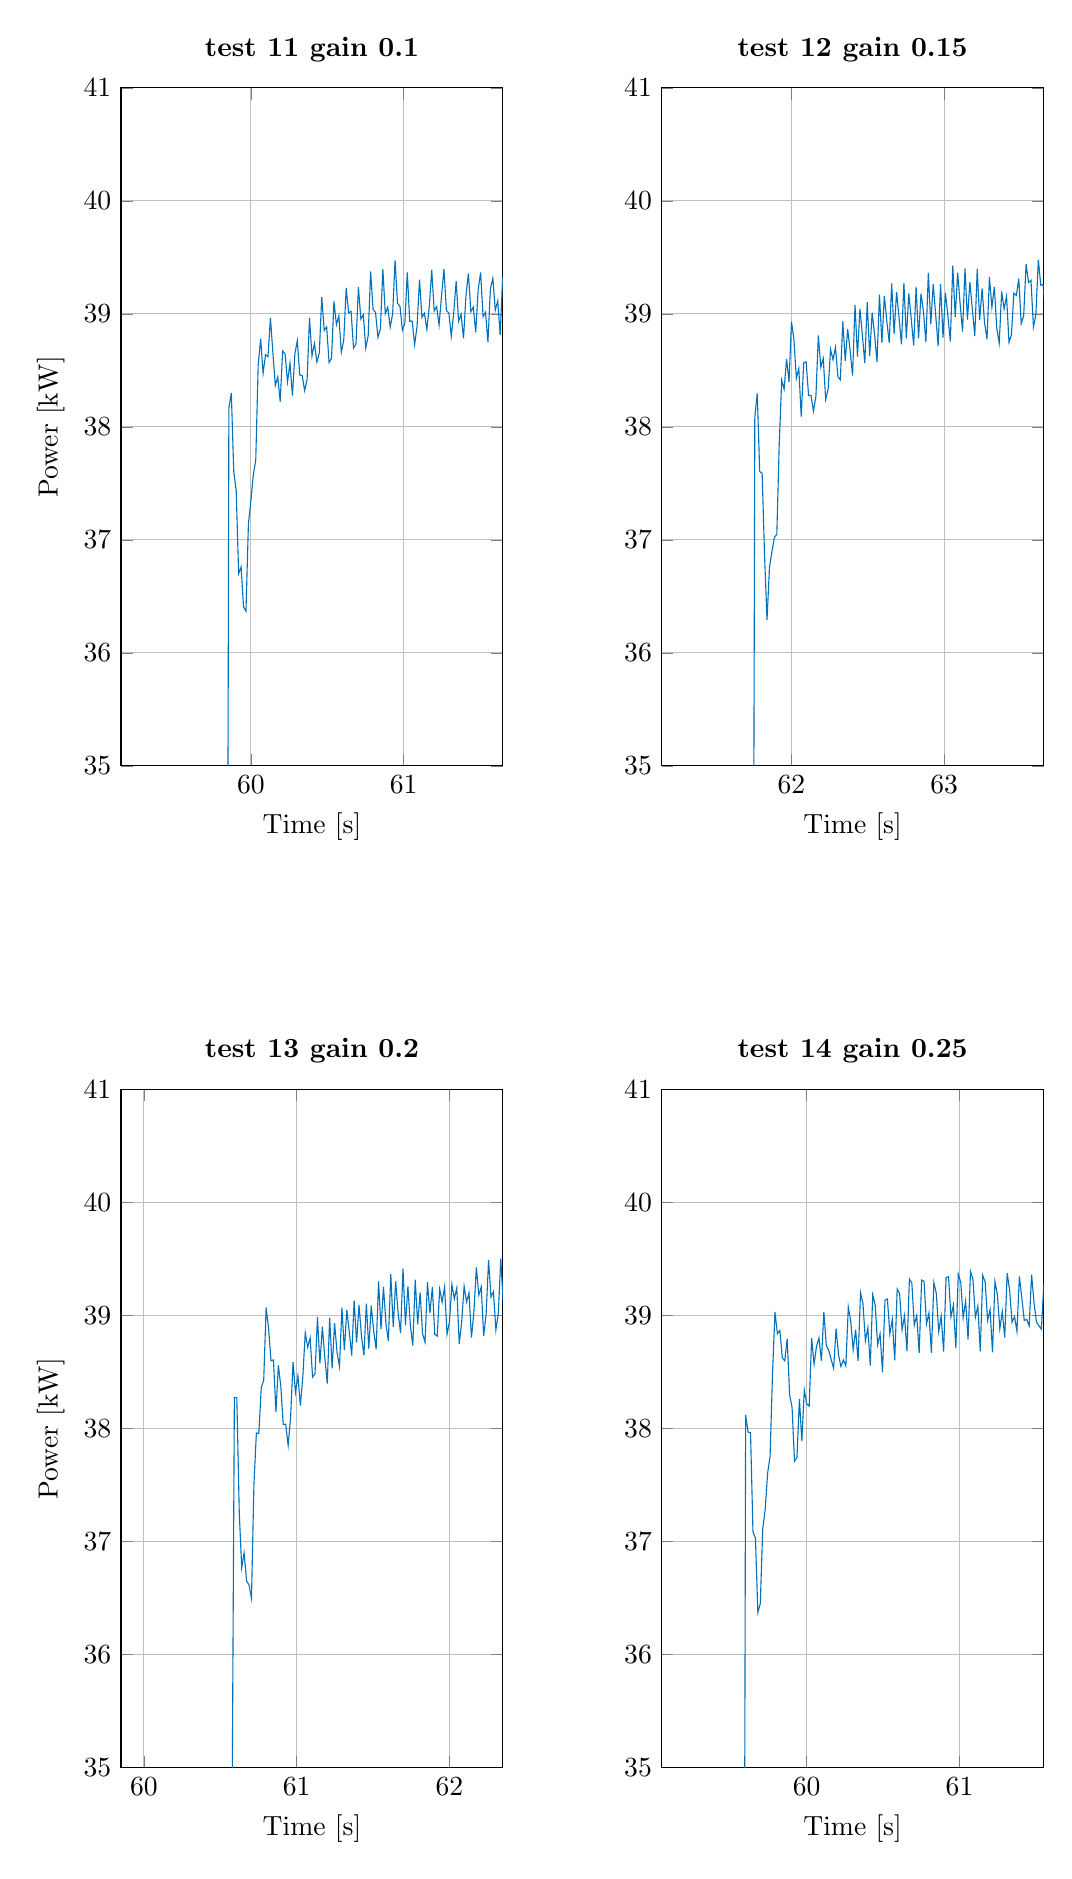
\begin{tikzpicture}

\begin{axis}[%
width=0.4\textwidth,
height=3.39in,
at={(1.297in,5.802in)},
scale only axis,
xmin=59.15,
xmax=61.65,
xlabel={Time [s]},
xmajorgrids,
ymin=35,
ymax=41,
ylabel={Power [kW]},
ymajorgrids,
axis background/.style={fill=white},
title style={font=\bfseries},
title={test 11 gain 0.1}
]
\addplot [color=mycolor1,solid,forget plot]
  table[row sep=crcr]{%
59.8492637646032	34.4\\
59.856	38.1660551256087\\
59.872	38.3004610292771\\
59.888	37.6022852869002\\
59.904	37.4325130195974\\
59.92	36.7011250985878\\
59.936	36.7587590576401\\
59.952	36.4070449326128\\
59.968	36.3689580338501\\
59.984	37.1429216841376\\
60	37.3430339886606\\
60.016	37.5754020756599\\
60.032	37.7065876095464\\
60.048	38.5491684059305\\
60.064	38.7803215936707\\
60.08	38.4739183784379\\
60.096	38.6395110590924\\
60.112	38.6211000319121\\
60.128	38.9647989037519\\
60.144	38.6573887932811\\
60.16	38.3651834013969\\
60.176	38.4428952958886\\
60.192	38.2233896071703\\
60.208	38.6711529801248\\
60.224	38.6443946922869\\
60.24	38.3986355973715\\
60.256	38.562248478259\\
60.272	38.2758392494933\\
60.288	38.6448324286704\\
60.304	38.7631795508432\\
60.32	38.4595527154756\\
60.336	38.454038101317\\
60.352	38.3210640544061\\
60.368	38.4184048399069\\
60.384	38.9636993438454\\
60.4	38.6286178839439\\
60.416	38.7378296421216\\
60.432	38.5742456595781\\
60.448	38.6561179881355\\
60.464	39.1505334920891\\
60.48	38.8525285652342\\
60.496	38.8845882795751\\
60.512	38.5704633501257\\
60.528	38.6087548630766\\
60.544	39.1105207102089\\
60.56	38.9045516718049\\
60.576	38.9826134960239\\
60.592	38.6606857783801\\
60.608	38.7675888377667\\
60.624	39.2302378944822\\
60.64	39.0084187928697\\
60.656	39.0224820500435\\
60.672	38.6966754796199\\
60.688	38.7330299980568\\
60.704	39.2355488421866\\
60.72	38.9543477057708\\
60.736	38.9929540402713\\
60.752	38.6965994715588\\
60.768	38.8070943997619\\
60.784	39.3765749529088\\
60.8	39.0389064169253\\
60.816	39.0130199764429\\
60.832	38.7913180105384\\
60.848	38.8666939384266\\
60.864	39.3983191769816\\
60.88	39.0004040633436\\
60.896	39.0594189750557\\
60.912	38.8817632568819\\
60.928	38.9999024715236\\
60.944	39.4738718231117\\
60.96	39.0934461483712\\
60.976	39.0679810465347\\
60.992	38.8550171646351\\
61.008	38.9167901103778\\
61.024	39.367867295155\\
61.04	38.9347025663566\\
61.056	38.936864333818\\
61.072	38.7278481665633\\
61.088	38.8887244734004\\
61.104	39.3033065263243\\
61.12	38.9687373784818\\
61.136	39.0060263440605\\
61.152	38.8626128462801\\
61.168	39.0657908117693\\
61.184	39.388222632162\\
61.2	39.0277880828573\\
61.216	39.0640274536213\\
61.232	38.9007344297963\\
61.248	39.1568893227392\\
61.264	39.3962803789277\\
61.28	39.0296430946185\\
61.296	39.0088497389118\\
61.312	38.8017858005023\\
61.328	39.0105144502165\\
61.344	39.2889507225367\\
61.36	38.9340153132789\\
61.376	38.9970482361951\\
61.392	38.7828433928086\\
61.408	39.1626664934166\\
61.424	39.3588699567146\\
61.44	39.0188476862886\\
61.456	39.0590393108992\\
61.472	38.8361110754645\\
61.488	39.2161180525256\\
61.504	39.3657009432625\\
61.52	38.9759935232161\\
61.536	39.0138906951821\\
61.552	38.7498907712266\\
61.568	39.2217645768995\\
61.584	39.3156752171705\\
61.6	39.0330341737601\\
61.616	39.1159175563737\\
61.632	38.8112506580535\\
61.648	39.316765939374\\
61.664	39.348273178182\\
};
\end{axis}

\begin{axis}[%
width=0.4\textwidth,
height=3.39in,
at={(4in,5.802in)},
scale only axis,
xmin=61.15,
xmax=63.65,
xlabel={Time [s]},
xmajorgrids,
ymin=35,
ymax=41,
ymajorgrids,
axis background/.style={fill=white},
title style={font=\bfseries},
title={test 12  gain 0.15}
]
\addplot [color=mycolor1,solid,forget plot]
  table[row sep=crcr]{%
61.7528825912593	34.4\\
61.76	38.083304511986\\
61.776	38.2953667033776\\
61.792	37.6071144608986\\
61.808	37.5867274769669\\
61.824	36.8554284775654\\
61.84	36.2917957616056\\
61.856	36.7546669356913\\
61.872	36.8949659706241\\
61.888	37.0202454213014\\
61.904	37.0489980216546\\
61.92	37.8487204057811\\
61.936	38.4137422828226\\
61.952	38.3352573932152\\
61.968	38.6021018866734\\
61.984	38.3962225966939\\
62	38.9305785058535\\
62.016	38.7758807352024\\
62.032	38.4289456665102\\
62.048	38.5171550206681\\
62.064	38.0910414786615\\
62.08	38.5662599008441\\
62.096	38.5754436467149\\
62.112	38.2786201216729\\
62.128	38.2770181198046\\
62.144	38.1395653189819\\
62.16	38.2707278088168\\
62.176	38.8095480186801\\
62.192	38.5290560483492\\
62.208	38.6057193623132\\
62.224	38.2417145350481\\
62.24	38.3341558132642\\
62.256	38.6838448202206\\
62.272	38.5951389663889\\
62.288	38.7032214240562\\
62.304	38.4439382635938\\
62.32	38.4168454356087\\
62.336	38.9336283048942\\
62.352	38.5851434496973\\
62.368	38.8644338561162\\
62.384	38.6737513997499\\
62.4	38.454635055318\\
62.416	39.0802330997982\\
62.432	38.6229782613098\\
62.448	39.0443829036092\\
62.464	38.8154417883714\\
62.48	38.5658330190327\\
62.496	39.1032431602479\\
62.512	38.6277578434903\\
62.528	39.0110564835912\\
62.544	38.8196840101967\\
62.56	38.5741147680865\\
62.576	39.169722053705\\
62.592	38.7429298843135\\
62.608	39.1591526079786\\
62.624	38.9366735814105\\
62.64	38.7448577583416\\
62.656	39.2686764019945\\
62.672	38.8215477428925\\
62.688	39.1949679816071\\
62.704	38.971815825858\\
62.72	38.7299769782425\\
62.736	39.2751053438335\\
62.752	38.7824521842951\\
62.768	39.1813281108851\\
62.784	38.9559413066366\\
62.8	38.7206313279926\\
62.816	39.2385411190364\\
62.832	38.7833509471\\
62.848	39.1795817044065\\
62.864	39.0209914291648\\
62.88	38.7507327304547\\
62.896	39.3636080177707\\
62.912	38.9099673296708\\
62.928	39.2637248553291\\
62.944	38.992122613724\\
62.96	38.7151404114942\\
62.976	39.2628033174286\\
62.992	38.7906503945359\\
63.008	39.1846631093354\\
63.024	38.9817187314502\\
63.04	38.7557960966733\\
63.056	39.4275362790954\\
63.072	38.9731146234457\\
63.088	39.3649256031932\\
63.104	39.0885188718155\\
63.12	38.8428198671295\\
63.136	39.4018018992976\\
63.152	38.9493816190021\\
63.168	39.2822794233757\\
63.184	39.0440700815027\\
63.2	38.803983062529\\
63.216	39.3972019517443\\
63.232	38.9455424450846\\
63.248	39.2243117586328\\
63.264	38.9205065374724\\
63.28	38.7770777650385\\
63.296	39.3239896005935\\
63.312	39.0584936191474\\
63.328	39.2386112799086\\
63.344	38.8720382531861\\
63.36	38.7416321824668\\
63.376	39.1978158274817\\
63.392	39.041946555134\\
63.408	39.1559804192551\\
63.424	38.7480078801814\\
63.44	38.8144606816068\\
63.456	39.1848195105116\\
63.472	39.162420228404\\
63.488	39.3104393861178\\
63.504	38.9147926250784\\
63.52	38.9813475963423\\
63.536	39.4425003133235\\
63.552	39.2773827289768\\
63.568	39.2961980235746\\
63.584	38.8830239818892\\
63.6	38.9947856357051\\
63.616	39.479966763089\\
63.632	39.2532821666541\\
63.648	39.2612120399381\\
63.664	38.9142647140247\\
};
\end{axis}

\begin{axis}[%
width=0.4\textwidth,
height=3.39in,
at={(1.297in,0.793in)},
scale only axis,
xmin=59.85,
xmax=62.35,
xlabel={Time [s]},
xmajorgrids,
ymin=35,
ymax=41,
ylabel={Power [kW]},
ymajorgrids,
axis background/.style={fill=white},
title style={font=\bfseries},
title={test 13  gain 0.2}
]
\addplot [color=mycolor1,solid,forget plot]
  table[row sep=crcr]{%
60.5762498584831	34.4\\
60.592	38.2761558323581\\
60.608	38.2729230309378\\
60.624	37.2593486833777\\
60.64	36.7688111651974\\
60.656	36.9017570534452\\
60.672	36.6509497656461\\
60.688	36.6168548513565\\
60.704	36.4981290972536\\
60.72	37.5045539604166\\
60.736	37.9622209378959\\
60.752	37.9579460234139\\
60.768	38.364075396425\\
60.784	38.4278203591703\\
60.8	39.0726112285821\\
60.816	38.8852034714879\\
60.832	38.6009410008281\\
60.848	38.6078045802003\\
60.864	38.1478251724931\\
60.88	38.5608282072348\\
60.896	38.3751129538195\\
60.912	38.0356363182606\\
60.928	38.0398248228528\\
60.944	37.8512472153401\\
60.96	38.0951783515423\\
60.976	38.5886338182708\\
60.992	38.322391324219\\
61.008	38.468188413996\\
61.024	38.2046240733224\\
61.04	38.4568293150843\\
61.056	38.8481881933773\\
61.072	38.7211410469072\\
61.088	38.8035322392096\\
61.104	38.4564669702851\\
61.12	38.4879144924511\\
61.136	38.9875870146848\\
61.152	38.5775698363205\\
61.168	38.901670796616\\
61.184	38.6287809878406\\
61.2	38.3990754785945\\
61.216	38.9799332454526\\
61.232	38.5336912278604\\
61.248	38.9343507108782\\
61.264	38.6758905779821\\
61.28	38.5488688122423\\
61.296	39.0709983046944\\
61.312	38.6947103361538\\
61.328	39.0510933663326\\
61.344	38.8630257529231\\
61.36	38.6472542577528\\
61.376	39.1355505608253\\
61.392	38.761283359896\\
61.408	39.0943645560208\\
61.424	38.8206426994382\\
61.44	38.6484565999956\\
61.456	39.1062246326538\\
61.472	38.7081658246307\\
61.488	39.0891054833449\\
61.504	38.8657061873003\\
61.52	38.702357169541\\
61.536	39.3032410636712\\
61.552	38.880307513924\\
61.568	39.2558814034302\\
61.584	38.9341681420268\\
61.6	38.7749317667891\\
61.616	39.3672006147242\\
61.632	38.8982913867986\\
61.648	39.3037678202541\\
61.664	39.0239808902375\\
61.68	38.8467826823205\\
61.696	39.4165155728132\\
61.712	38.9172782105641\\
61.728	39.2592691803044\\
61.744	38.9158292011998\\
61.76	38.7352408219798\\
61.776	39.317684177211\\
61.792	38.9224373307643\\
61.808	39.205342670138\\
61.824	38.8389527377121\\
61.84	38.7654648884783\\
61.856	39.2954933746083\\
61.872	39.0236090645678\\
61.888	39.2514338397443\\
61.904	38.8352723152541\\
61.92	38.8197975673798\\
61.936	39.2349061344353\\
61.952	39.1212210620241\\
61.968	39.2540044528057\\
61.984	38.8347697166346\\
62	38.9443079703739\\
62.016	39.2764866638526\\
62.032	39.1492568265955\\
62.048	39.2454863667004\\
62.064	38.7509088321333\\
62.08	38.9434707168896\\
62.096	39.2598795509708\\
62.112	39.1210143750881\\
62.128	39.2012000296855\\
62.144	38.8054331870185\\
62.16	39.0319148075194\\
62.176	39.4276111379853\\
62.192	39.1816554290437\\
62.208	39.2548399393269\\
62.224	38.8192316417107\\
62.24	39.0118591666372\\
62.256	39.4904447703495\\
62.272	39.1654835092281\\
62.288	39.2127265000248\\
62.304	38.8745990151232\\
62.32	39.0211732863863\\
62.336	39.5050856643882\\
62.352	39.1106876527107\\
};
\end{axis}

\begin{axis}[%
width=0.4\textwidth,
height=3.39in,
at={(4in,0.793in)},
scale only axis,
xmin=59.05,
xmax=61.55,
xlabel={Time [s]},
xmajorgrids,
ymin=35,
ymax=41,
ymajorgrids,
axis background/.style={fill=white},
title style={font=\bfseries},
title={test 14  gain 0.25}
]
\addplot [color=mycolor1,solid,forget plot]
  table[row sep=crcr]{%
59.5932281329978	34.4\\
59.6	38.1211102937107\\
59.616	37.9696920026539\\
59.632	37.9638707090714\\
59.648	37.0874982811597\\
59.664	37.0345501683713\\
59.68	36.3744045737014\\
59.696	36.4525076123853\\
59.712	37.1146759921158\\
59.728	37.2853429979972\\
59.744	37.6082278353144\\
59.76	37.7547504149765\\
59.776	38.4918991097659\\
59.792	39.033162055273\\
59.808	38.8404346703955\\
59.824	38.8691826566896\\
59.84	38.6266163994654\\
59.856	38.5999472228243\\
59.872	38.7943492304097\\
59.888	38.2992342661078\\
59.904	38.187057091897\\
59.92	37.712295352502\\
59.936	37.7449892753841\\
59.952	38.2637041511549\\
59.968	37.8898125179335\\
59.984	38.3417027480028\\
60	38.2180772076361\\
60.016	38.199287309287\\
60.032	38.8007062063527\\
60.048	38.5705924090299\\
60.064	38.7305779009654\\
60.08	38.8020730702554\\
60.096	38.6009791679097\\
60.112	39.0335135375392\\
60.128	38.73511693906\\
60.144	38.6930172321798\\
60.16	38.6109153970274\\
60.176	38.5328371501174\\
60.192	38.8860997100463\\
60.208	38.654386045981\\
60.224	38.5498761202729\\
60.24	38.6081616613206\\
60.256	38.5550956109147\\
60.272	39.07736250624\\
60.288	38.9513736319687\\
60.304	38.6990163732177\\
60.32	38.8751349512693\\
60.336	38.5983102199614\\
60.352	39.2043975655397\\
60.368	39.1066608788126\\
60.384	38.776861137081\\
60.4	38.8941770396755\\
60.416	38.5582296388108\\
60.432	39.1853546695174\\
60.448	39.0960697299137\\
60.464	38.7429539910861\\
60.48	38.8381127042783\\
60.496	38.4988022432692\\
60.512	39.1369723555318\\
60.528	39.1471743560185\\
60.544	38.839350859706\\
60.56	38.9662074784028\\
60.576	38.6036195125561\\
60.592	39.2350781779364\\
60.608	39.1946709779236\\
60.624	38.8743819701324\\
60.64	38.9986495765469\\
60.656	38.6858069443177\\
60.672	39.3242432219969\\
60.688	39.2908947867377\\
60.704	38.9152240921363\\
60.72	39.0021262771221\\
60.736	38.6687834718569\\
60.752	39.3152247859977\\
60.768	39.3027447419016\\
60.784	38.9284693663734\\
60.8	39.023255857857\\
60.816	38.6716848977932\\
60.832	39.2935719087506\\
60.848	39.1987752697688\\
60.864	38.8599800899011\\
60.88	38.9951373771833\\
60.896	38.6819985874361\\
60.912	39.3368895612105\\
60.928	39.3437693863316\\
60.944	38.9897807342224\\
60.96	39.0924447726188\\
60.976	38.7130088794244\\
60.992	39.368212182679\\
61.008	39.2953169681214\\
61.024	38.9815501633888\\
61.04	39.1293951781772\\
61.056	38.7895208294257\\
61.072	39.3929657069728\\
61.088	39.3202114634413\\
61.104	38.9870813364254\\
61.12	39.0837151108632\\
61.136	38.6835511780728\\
61.152	39.3558951875764\\
61.168	39.298551945263\\
61.184	38.9581906958985\\
61.2	39.0539661504937\\
61.216	38.6758971868148\\
61.232	39.3029946844734\\
61.248	39.1875146720997\\
61.264	38.8837376898106\\
61.28	39.0368138122364\\
61.296	38.8069325987866\\
61.312	39.3767003134232\\
61.328	39.226711451462\\
61.344	38.9412183053755\\
61.36	38.9920009949789\\
61.376	38.8616531192709\\
61.392	39.3478040659654\\
61.408	39.1570824907085\\
61.424	38.9580846989434\\
61.44	38.9671550764307\\
61.456	38.9088670129476\\
61.472	39.363764867596\\
61.488	39.1102088767688\\
61.504	38.9441961784345\\
61.52	38.9097527156141\\
61.536	38.8818544557807\\
61.552	39.2794724236294\\
};
\end{axis}
\end{tikzpicture}%
\caption{Step from 30 to 40 kW load, with various scaling factors.}
\label{fig:test11-14-30to40kwsteppower}
\end{figure}

\begin{figure}[H]
\centering
% This file was created by matlab2tikz.
%
%The latest updates can be retrieved from
%  http://www.mathworks.com/matlabcentral/fileexchange/22022-matlab2tikz-matlab2tikz
%where you can also make suggestions and rate matlab2tikz.
%
\definecolor{mycolor1}{rgb}{0.00000,0.44700,0.74100}%
%
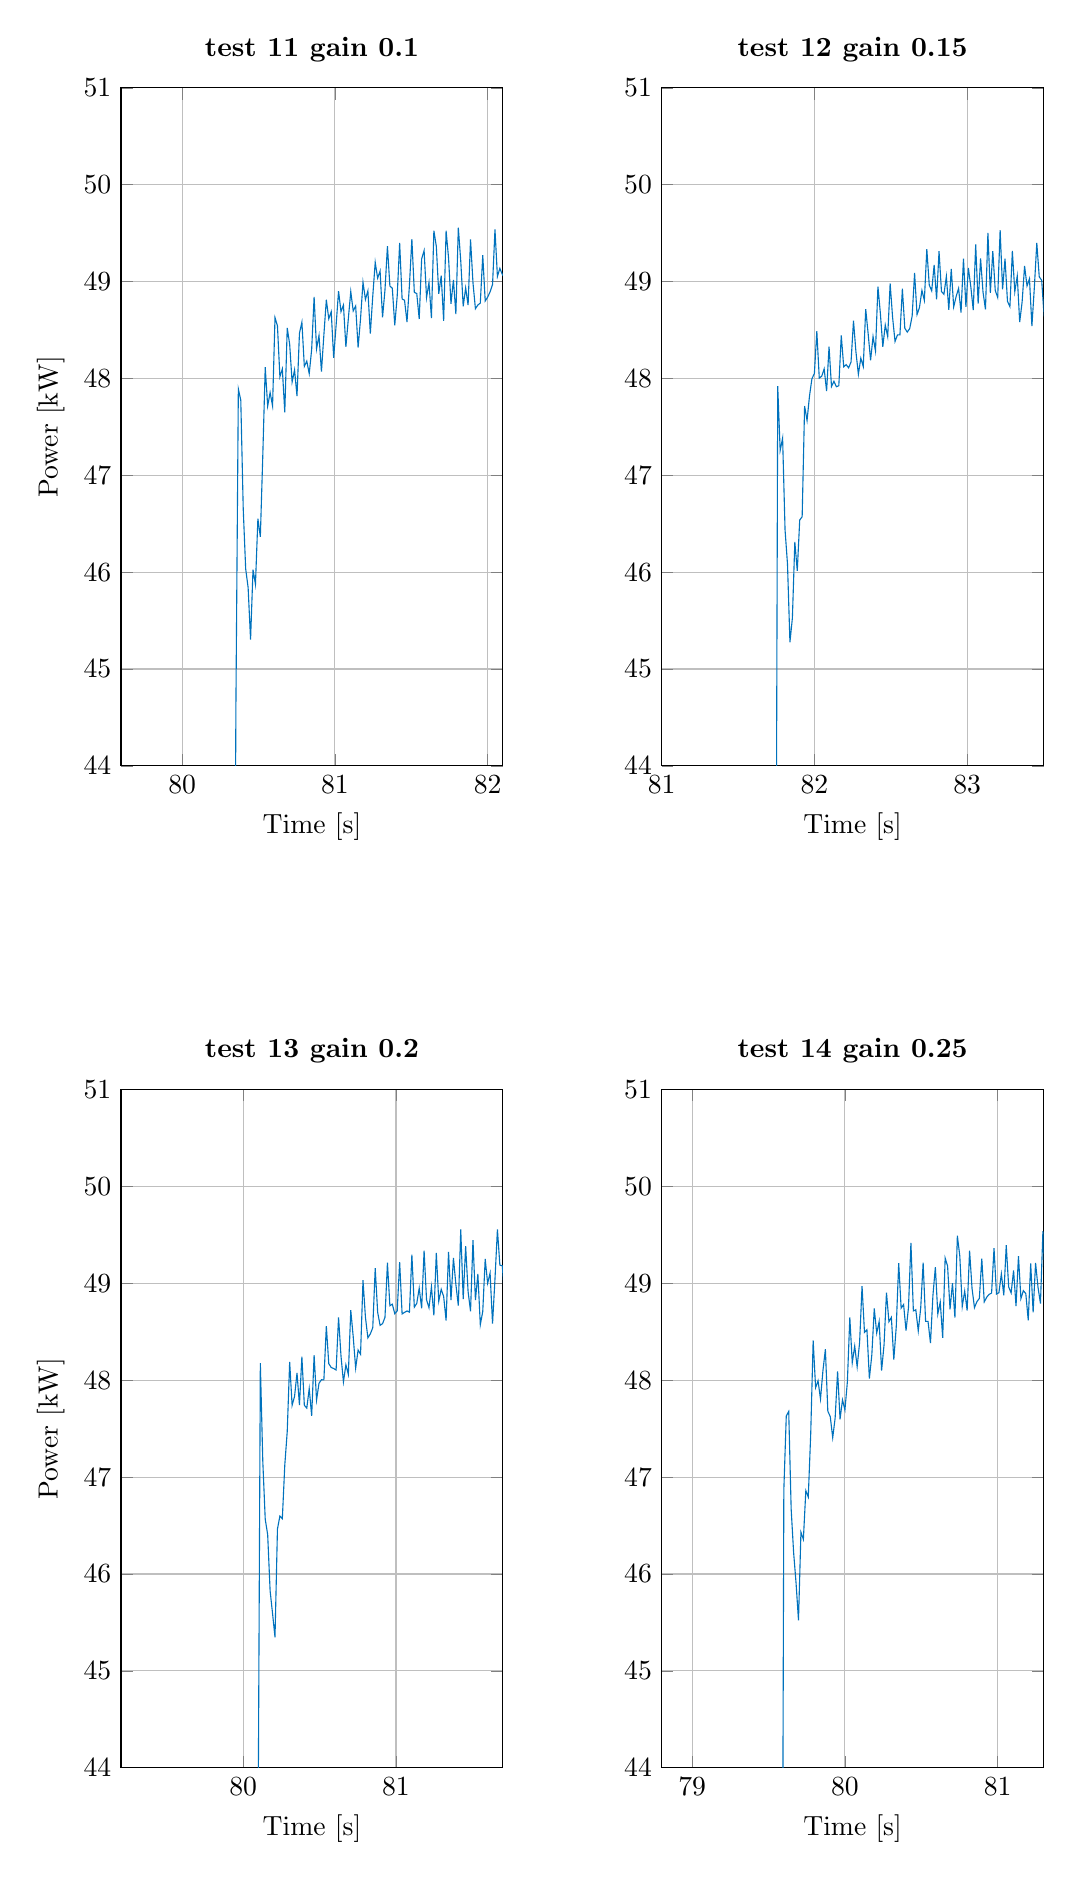
\begin{tikzpicture}

\begin{axis}[%
width=0.4\textwidth,
height=3.39in,
at={(1.297in,5.802in)},
scale only axis,
xmin=79.6,
xmax=82.1,
xlabel={Time [s]},
xmajorgrids,
ymin=44,
ymax=51,
ylabel={Power [kW]},
ymajorgrids,
axis background/.style={fill=white},
title style={font=\bfseries},
title={test 11 gain 0.1}
]
\addplot [color=mycolor1,solid,forget plot]
  table[row sep=crcr]{%
80.3482518358082	43.3\\
80.352	44.6012366130227\\
80.368	47.8915034390884\\
80.384	47.7752911997672\\
80.4	46.6530651261051\\
80.416	46.034714647916\\
80.432	45.8403088195061\\
80.448	45.3027666060487\\
80.464	46.0263102840445\\
80.48	45.8742372256547\\
80.496	46.5530914491379\\
80.512	46.3648839920262\\
80.528	47.2002744802701\\
80.544	48.1170060724637\\
80.56	47.7144653510928\\
80.576	47.8545716254597\\
80.592	47.7167157890807\\
80.608	48.6281955850112\\
80.624	48.5427184849617\\
80.64	48.0175087264892\\
80.656	48.0977321028934\\
80.672	47.6501762526095\\
80.688	48.5221389923473\\
80.704	48.3529768305024\\
80.72	47.9623293590454\\
80.736	48.0880928732353\\
80.752	47.8167219170864\\
80.768	48.465914789242\\
80.784	48.5807433136921\\
80.8	48.1250417647484\\
80.816	48.1792351008494\\
80.832	48.0490085577922\\
80.848	48.3002699238648\\
80.864	48.8417186847136\\
80.88	48.305819001427\\
80.896	48.4431232112622\\
80.912	48.070332605286\\
80.928	48.4512390265193\\
80.944	48.8119499125082\\
80.96	48.615610232903\\
80.976	48.6895146844969\\
80.992	48.2130713968021\\
81.008	48.5494805732881\\
81.024	48.9020926409915\\
81.04	48.6893753581569\\
81.056	48.7579806704117\\
81.072	48.3257307567801\\
81.088	48.6159084714271\\
81.104	48.8969904270247\\
81.12	48.6966026259533\\
81.136	48.7480776060203\\
81.152	48.3194087524265\\
81.168	48.6182331690225\\
81.184	48.993923343961\\
81.2	48.8156403589377\\
81.216	48.9046302601672\\
81.232	48.4629390218514\\
81.248	48.8511650388433\\
81.264	49.1987091678537\\
81.28	49.0352320837328\\
81.296	49.1091030800248\\
81.312	48.6298538318822\\
81.328	48.9151095411613\\
81.344	49.365631466625\\
81.36	48.9545997988066\\
81.376	48.930994954337\\
81.392	48.5487831572822\\
81.408	48.8520284368743\\
81.424	49.3982430557725\\
81.44	48.8210192211993\\
81.456	48.8074090163986\\
81.472	48.5819143503407\\
81.488	48.9626323465829\\
81.504	49.4388707037085\\
81.52	48.8893558040304\\
81.536	48.8761603115166\\
81.552	48.6140984593618\\
81.568	49.2343984716617\\
81.584	49.3197562776346\\
81.6	48.8350021426763\\
81.616	48.9894729025122\\
81.632	48.6230513870957\\
81.648	49.5259396319068\\
81.664	49.3641590488692\\
81.68	48.8746214306822\\
81.696	49.0601425234316\\
81.712	48.59453302363\\
81.728	49.5245529582525\\
81.744	49.2476599682407\\
81.76	48.7708068260473\\
81.776	49.0173871809286\\
81.792	48.6643662755175\\
81.808	49.5573871197449\\
81.824	49.2125784683807\\
81.84	48.7441239005751\\
81.856	48.9345799493542\\
81.872	48.7566185423152\\
81.888	49.434616870366\\
81.904	48.9870281768308\\
81.92	48.7196809410022\\
81.936	48.757965541393\\
81.952	48.7780771752851\\
81.968	49.2728280038676\\
81.984	48.7998626075211\\
82	48.8385120349759\\
82.016	48.8945209601903\\
82.032	48.9682880913931\\
82.048	49.5379684252861\\
82.064	49.0531321280057\\
82.08	49.1367776508318\\
82.096	49.0744327535071\\
82.112	49.0348777755488\\
};
\end{axis}

\begin{axis}[%
width=0.4\textwidth,
height=3.39in,
at={(4in,5.802in)},
scale only axis,
xmin=81,
xmax=83.5,
xlabel={Time [s]},
xmajorgrids,
ymin=44,
ymax=51,
ymajorgrids,
axis background/.style={fill=white},
title style={font=\bfseries},
title={test 12  gain 0.15}
]
\addplot [color=mycolor1,solid,forget plot]
  table[row sep=crcr]{%
81.7510274793404	43.3\\
81.76	47.9209261403146\\
81.776	47.2566174184142\\
81.792	47.3843157010726\\
81.808	46.436630378583\\
81.824	46.0835466278897\\
81.84	45.2766244924613\\
81.856	45.5260922936217\\
81.872	46.3114419142901\\
81.888	46.0139599850132\\
81.904	46.5380103992794\\
81.92	46.5724991925889\\
81.936	47.7149066360685\\
81.952	47.5656390831491\\
81.968	47.818771974683\\
81.984	47.9978163520659\\
82	48.0492002233048\\
82.016	48.4875864034556\\
82.032	48.0031449548023\\
82.048	48.0233526920218\\
82.064	48.0992911635156\\
82.08	47.8692560268157\\
82.096	48.3283945500737\\
82.112	47.9166888262892\\
82.128	47.9702888578052\\
82.144	47.9144479956414\\
82.16	47.9249135173449\\
82.176	48.4450079456755\\
82.192	48.1204502181487\\
82.208	48.1421450392023\\
82.224	48.1098736199624\\
82.24	48.1694178136568\\
82.256	48.5963257475029\\
82.272	48.2743284457068\\
82.288	48.0430053151114\\
82.304	48.2093759583979\\
82.32	48.1224433172225\\
82.336	48.7160300331951\\
82.352	48.4616518474111\\
82.368	48.1876996462109\\
82.384	48.4326253522761\\
82.4	48.2829179124986\\
82.416	48.9482678416164\\
82.432	48.6706191254818\\
82.448	48.3266969479064\\
82.464	48.5523484015608\\
82.48	48.4321547494477\\
82.496	48.9802903515608\\
82.512	48.6299871875843\\
82.528	48.3816149046718\\
82.544	48.4498154522422\\
82.56	48.4490906072072\\
82.576	48.9259678022835\\
82.592	48.5184432549715\\
82.608	48.4784576732333\\
82.624	48.5145603249894\\
82.64	48.6439020464191\\
82.656	49.0885382708763\\
82.672	48.6590471034083\\
82.688	48.7336173206646\\
82.704	48.9087101406868\\
82.72	48.8069295589016\\
82.736	49.3357525507192\\
82.752	48.9647785014543\\
82.768	48.904343962848\\
82.784	49.1727043476963\\
82.8	48.8156315072599\\
82.816	49.3135563956916\\
82.832	48.8979891112326\\
82.848	48.8688936820189\\
82.864	49.0530162790174\\
82.88	48.7089258954125\\
82.896	49.1312751371382\\
82.912	48.7386369969355\\
82.928	48.8461652989956\\
82.944	48.930003325242\\
82.96	48.6792293732132\\
82.976	49.2373413516189\\
82.992	48.7389485331565\\
83.008	49.1406428276816\\
83.024	48.9474757410405\\
83.04	48.7047034617164\\
83.056	49.3836521407213\\
83.072	48.7727376588409\\
83.088	49.2381796833506\\
83.104	48.8900778376678\\
83.12	48.712448385801\\
83.136	49.5035120390326\\
83.152	48.8824771441476\\
83.168	49.3142129622555\\
83.184	48.9090417566439\\
83.2	48.8359683673171\\
83.216	49.5318679414865\\
83.232	48.9196843790035\\
83.248	49.2369509119296\\
83.264	48.7967372614159\\
83.28	48.7410458342529\\
83.296	49.3164373155158\\
83.312	48.8960366382194\\
83.328	49.0580399341387\\
83.344	48.581182596555\\
83.36	48.7907669366202\\
83.376	49.16181313715\\
83.392	48.9551620547585\\
83.408	49.0304001450578\\
83.424	48.5399205299024\\
83.44	48.9399900735255\\
83.456	49.3999993436816\\
83.472	49.0488877214749\\
83.488	49.0138496783674\\
83.504	48.6361706248948\\
};
\end{axis}

\begin{axis}[%
width=0.4\textwidth,
height=3.39in,
at={(1.297in,0.793in)},
scale only axis,
xmin=79.2,
xmax=81.7,
xlabel={Time [s]},
xmajorgrids,
ymin=44,
ymax=51,
ylabel={Power [kW]},
ymajorgrids,
axis background/.style={fill=white},
title style={font=\bfseries},
title={test 13  gain 0.2}
]
\addplot [color=mycolor1,solid,forget plot]
  table[row sep=crcr]{%
80.0972485601229	43.3\\
80.112	48.1765105083361\\
80.128	47.1663550488153\\
80.144	46.5649771017343\\
80.16	46.406521217309\\
80.176	45.8261204521389\\
80.192	45.59045368623\\
80.208	45.3462131765881\\
80.224	46.4633870304378\\
80.24	46.5983025398771\\
80.256	46.5707252621494\\
80.272	47.1226875530313\\
80.288	47.4698724454034\\
80.304	48.1893879531735\\
80.32	47.7413765153744\\
80.336	47.8333266483289\\
80.352	48.0752587227737\\
80.368	47.7446662675501\\
80.384	48.2429757422938\\
80.4	47.7421027047267\\
80.416	47.7119223449584\\
80.432	47.9134445540899\\
80.448	47.6317066677588\\
80.464	48.2585090091182\\
80.48	47.7967916264415\\
80.496	47.968297168473\\
80.512	48.0050476318716\\
80.528	48.003702374619\\
80.544	48.5593763143589\\
80.56	48.1707133072916\\
80.576	48.1317269191035\\
80.592	48.1209094783648\\
80.608	48.1059937310257\\
80.624	48.6485286553292\\
80.64	48.2499236555099\\
80.656	47.9822226231949\\
80.672	48.1591037592701\\
80.688	48.0610593380688\\
80.704	48.7228542157519\\
80.72	48.4490228191258\\
80.736	48.1248936249111\\
80.752	48.3122879248526\\
80.768	48.2684099880803\\
80.784	49.0322286527854\\
80.8	48.6504190730535\\
80.816	48.4378893349446\\
80.832	48.4782597127225\\
80.848	48.5429236797519\\
80.864	49.1572179752469\\
80.88	48.7015559194293\\
80.896	48.5668870878178\\
80.912	48.5836187770552\\
80.928	48.6500388133228\\
80.944	49.213192519518\\
80.96	48.769037523598\\
80.976	48.785651167717\\
80.992	48.6867628655832\\
81.008	48.7168200130043\\
81.024	49.2202388708523\\
81.04	48.6844248448892\\
81.056	48.700609235406\\
81.072	48.7150300664643\\
81.088	48.70243859681\\
81.104	49.2965957128558\\
81.12	48.7542138012825\\
81.136	48.793733096341\\
81.152	48.9506422797655\\
81.168	48.7429155749744\\
81.184	49.3389005208776\\
81.2	48.8304209844484\\
81.216	48.7485522595523\\
81.232	48.96435054089\\
81.248	48.6697247194122\\
81.264	49.3146230255281\\
81.28	48.8158323483481\\
81.296	48.9388086070395\\
81.312	48.8657591380993\\
81.328	48.6162883518944\\
81.344	49.3256202313365\\
81.36	48.8267886674877\\
81.376	49.2635233238547\\
81.392	48.9895851096647\\
81.408	48.7700314616363\\
81.424	49.5564562377529\\
81.44	48.8380509964609\\
81.456	49.3853861645755\\
81.472	48.9141505483762\\
81.488	48.7123756904226\\
81.504	49.4475361796131\\
81.52	48.8266428510682\\
81.536	49.0979093918109\\
81.552	48.5732158029818\\
81.568	48.7104335922317\\
81.584	49.2515165588809\\
81.6	49.0010591759671\\
81.616	49.1069212385226\\
81.632	48.5838316771528\\
81.648	49.0437283363865\\
81.664	49.5571958872729\\
81.68	49.1890040750886\\
81.696	49.1811349839864\\
81.712	48.8234304937055\\
};
\end{axis}

\begin{axis}[%
width=0.4\textwidth,
height=3.39in,
at={(4in,0.793in)},
scale only axis,
xmin=78.8,
xmax=81.3,
xlabel={Time [s]},
xmajorgrids,
ymin=44,
ymax=51,
ymajorgrids,
axis background/.style={fill=white},
title style={font=\bfseries},
title={test 14  gain 0.25}
]
\addplot [color=mycolor1,solid,forget plot]
  table[row sep=crcr]{%
79.5928371904828	43.3\\
79.6	46.8644936821218\\
79.616	47.6309469840876\\
79.632	47.6781202448495\\
79.648	46.6709470765757\\
79.664	46.2233485999663\\
79.68	45.9074000337815\\
79.696	45.5208935672749\\
79.712	46.430399515517\\
79.728	46.358213898122\\
79.744	46.8599902622232\\
79.76	46.7945007130901\\
79.776	47.4457558510253\\
79.792	48.4110755641038\\
79.808	47.9239560004817\\
79.824	47.9945759519927\\
79.84	47.8062656725235\\
79.856	48.0986996245919\\
79.872	48.3201583159975\\
79.888	47.6814641749326\\
79.904	47.6241602752089\\
79.92	47.4067361547468\\
79.936	47.6111612437399\\
79.952	48.0923783591619\\
79.968	47.5975052814814\\
79.984	47.7972349291428\\
80	47.6931820849425\\
80.016	47.9841892106037\\
80.032	48.6482987573869\\
80.048	48.1815053554995\\
80.064	48.3520097948158\\
80.08	48.1390370280804\\
80.096	48.3885358299994\\
80.112	48.9716395069743\\
80.128	48.4949786076804\\
80.144	48.5212329725142\\
80.16	48.0177773971504\\
80.176	48.2608731430737\\
80.192	48.7409158284166\\
80.208	48.4875318114457\\
80.224	48.6065947946148\\
80.24	48.0992391958726\\
80.256	48.3656565034539\\
80.272	48.9046964571377\\
80.288	48.6046658379953\\
80.304	48.6490369521703\\
80.32	48.2135690785119\\
80.336	48.5538687155479\\
80.352	49.2089393828264\\
80.368	48.7444991476316\\
80.384	48.7811904667836\\
80.4	48.5119509856812\\
80.416	48.7504911821703\\
80.432	49.4178743687366\\
80.448	48.7157626264024\\
80.464	48.7274423728462\\
80.48	48.5093582576828\\
80.496	48.74562545766\\
80.512	49.2136207339824\\
80.528	48.6083460261934\\
80.544	48.6077471947822\\
80.56	48.3836751957141\\
80.576	48.8744237946122\\
80.592	49.1685639435002\\
80.608	48.6833944502686\\
80.624	48.8077595205179\\
80.64	48.4369466393332\\
80.656	49.2619012342291\\
80.672	49.1792257100793\\
80.688	48.7327775554854\\
80.704	49.001012385337\\
80.72	48.6474313088883\\
80.736	49.4924776925254\\
80.752	49.2813305524663\\
80.768	48.761618280289\\
80.784	48.9206490912787\\
80.8	48.7203146447542\\
80.816	49.3386969744319\\
80.832	48.9491993715989\\
80.848	48.7497178970517\\
80.864	48.8115940422582\\
80.88	48.8450015723781\\
80.896	49.2557667360872\\
80.912	48.80853848887\\
80.928	48.8568145405256\\
80.944	48.8871888177128\\
80.96	48.8998425604365\\
80.976	49.3635057181539\\
80.992	48.8900503762177\\
81.008	48.9035721127058\\
81.024	49.0981585792763\\
81.04	48.8766907939125\\
81.056	49.3937559781591\\
81.072	48.9634855336437\\
81.088	48.9011380568614\\
81.104	49.1346326530763\\
81.12	48.766556437279\\
81.136	49.2812592410762\\
81.152	48.842886271621\\
81.168	48.9250580341004\\
81.184	48.8945166104009\\
81.2	48.6186199590625\\
81.216	49.2055976046547\\
81.232	48.7011389231922\\
81.248	49.2112172065769\\
81.264	48.9595098668816\\
81.28	48.7921560445649\\
81.296	49.5386386461124\\
81.312	48.9048882633957\\
};
\end{axis}
\end{tikzpicture}%
\caption{Step from 40 to 50 kW load, with various scaling factors.}
\label{fig:test11-14-40to50kwsteppower}
\end{figure}

\begin{figure}[H]
\centering
% This file was created by matlab2tikz.
%
%The latest updates can be retrieved from
%  http://www.mathworks.com/matlabcentral/fileexchange/22022-matlab2tikz-matlab2tikz
%where you can also make suggestions and rate matlab2tikz.
%
\definecolor{mycolor1}{rgb}{0.00000,0.44700,0.74100}%
%
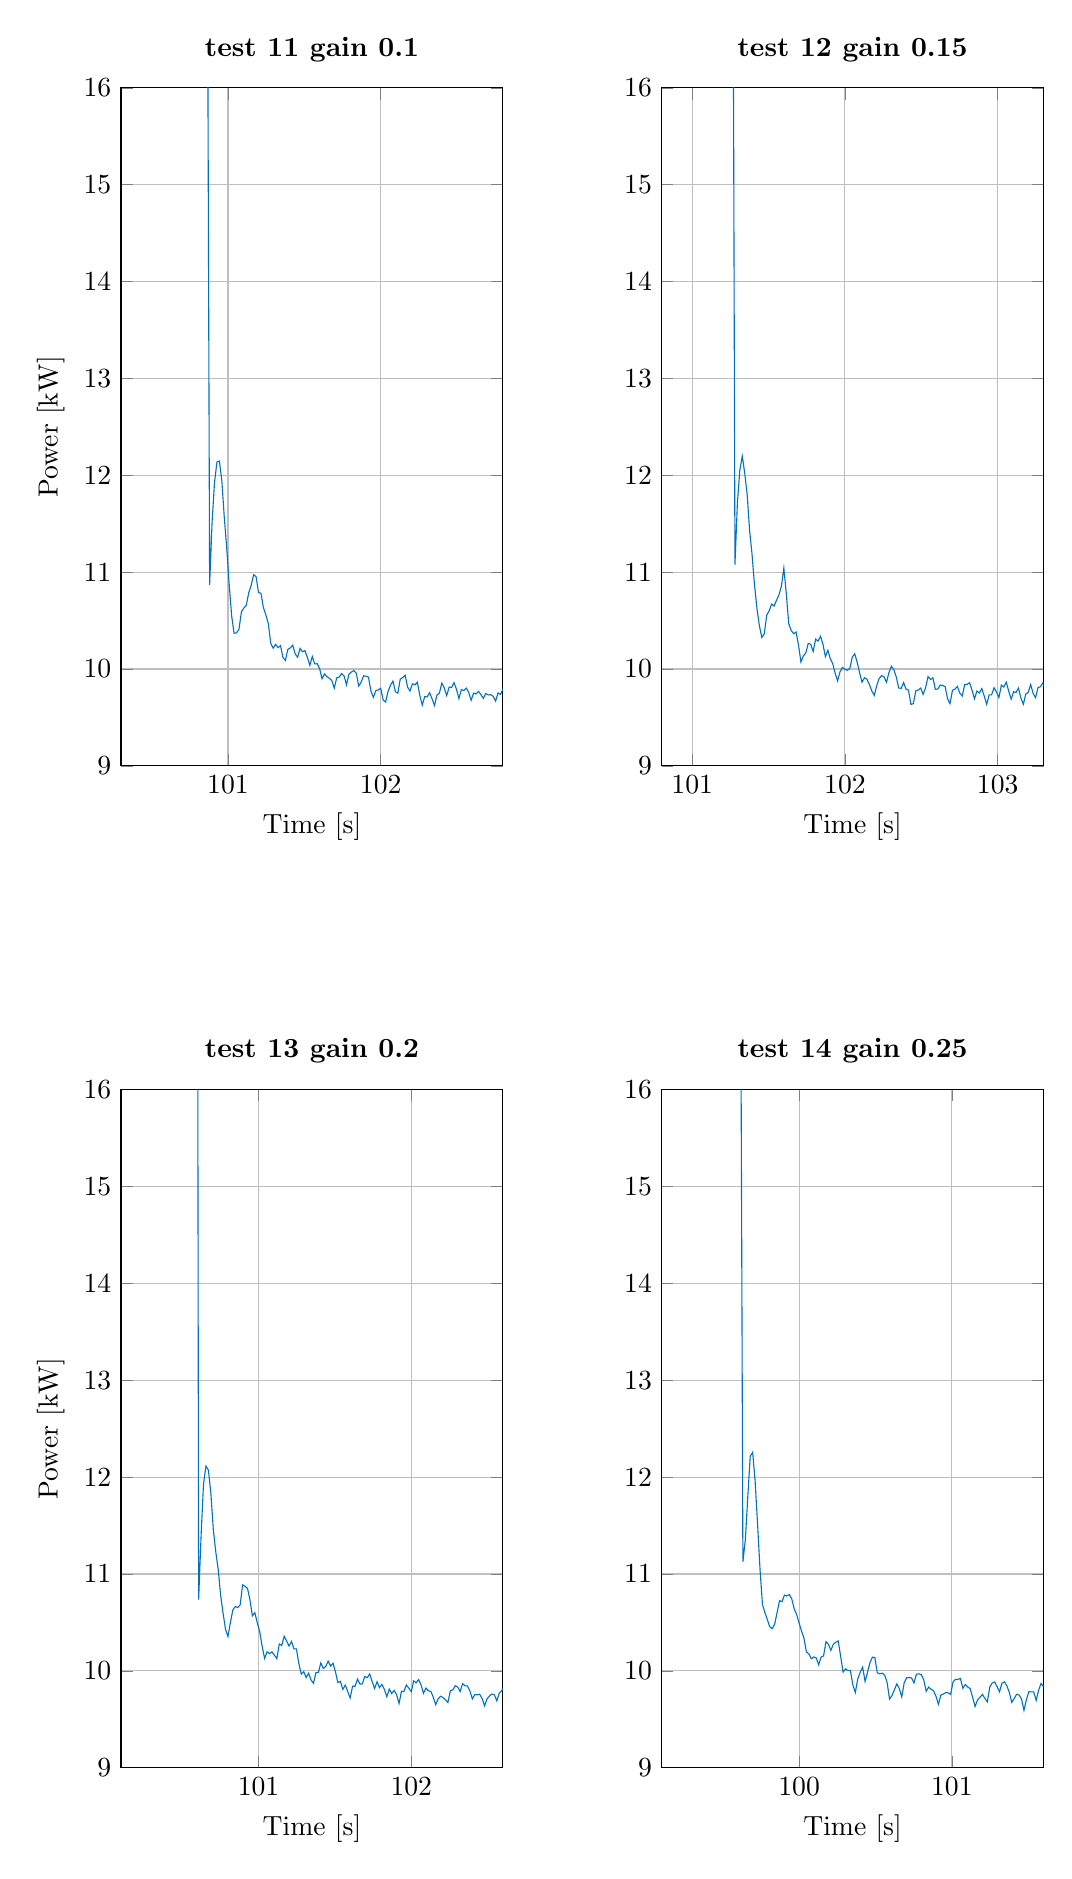
\begin{tikzpicture}

\begin{axis}[%
width=0.4\textwidth,
height=3.39in,
at={(1.297in,5.802in)},
scale only axis,
xmin=100.3,
xmax=102.8,
xlabel={Time [s]},
xmajorgrids,
ymin=9,
ymax=16,
ylabel={Power [kW]},
ymajorgrids,
axis background/.style={fill=white},
title style={font=\bfseries},
title={test 11 gain 0.1}
]
\addplot [color=mycolor1,solid,forget plot]
  table[row sep=crcr]{%
100.867563546396	16.7\\
100.88	10.8680114590886\\
100.896	11.5141228828877\\
100.912	11.9234322332521\\
100.928	12.1375625315368\\
100.944	12.1464303926376\\
100.96	11.9425508289521\\
100.976	11.5646538004679\\
100.992	11.2473476420234\\
101.008	10.8753572266415\\
101.024	10.5504659403249\\
101.04	10.3693801061788\\
101.056	10.3726588147923\\
101.072	10.410469545497\\
101.088	10.5891490821405\\
101.104	10.6299580330395\\
101.12	10.6582445217783\\
101.136	10.7877872960056\\
101.152	10.8628122146273\\
101.168	10.9738989297439\\
101.184	10.9535992911334\\
101.2	10.7901243073875\\
101.216	10.7813408430229\\
101.232	10.6332018371168\\
101.248	10.5592278790561\\
101.264	10.4710061807094\\
101.28	10.2665148665393\\
101.296	10.2150117500202\\
101.312	10.2544918763883\\
101.328	10.2204803728427\\
101.344	10.2417385725446\\
101.36	10.1196623355453\\
101.376	10.0882908866917\\
101.392	10.20256548195\\
101.408	10.2179189208091\\
101.424	10.2464713296238\\
101.44	10.1559306488497\\
101.456	10.1213592428516\\
101.472	10.2126705749898\\
101.488	10.1783429807813\\
101.504	10.189969050639\\
101.52	10.1192793024694\\
101.536	10.0386053665772\\
101.552	10.1284327914161\\
101.568	10.0529152585234\\
101.584	10.0542753934684\\
101.6	10.0051925279731\\
101.616	9.89818786596518\\
101.632	9.95039611063447\\
101.648	9.92043744797648\\
101.664	9.9039324020748\\
101.68	9.88123772589184\\
101.696	9.80256470819921\\
101.712	9.90871330440443\\
101.728	9.91577367692766\\
101.744	9.95240355765504\\
101.76	9.92851276172224\\
101.776	9.83822501077004\\
101.792	9.94666199271129\\
101.808	9.96878399744627\\
101.824	9.98395013826464\\
101.84	9.95770451855013\\
101.856	9.82460724397554\\
101.872	9.86392568765032\\
101.888	9.93000237896528\\
101.904	9.92543931487112\\
101.92	9.91595245788728\\
101.936	9.77073716185381\\
101.952	9.70765704648794\\
101.968	9.77637346429599\\
101.984	9.78407358788574\\
102	9.80166210536905\\
102.016	9.67950905891732\\
102.032	9.65848877963446\\
102.048	9.76890317133189\\
102.064	9.83173707935773\\
102.08	9.87581061734866\\
102.096	9.76685756998541\\
102.112	9.75027222620253\\
102.128	9.89588320451701\\
102.144	9.91124103200347\\
102.16	9.93627965692971\\
102.176	9.81279398865476\\
102.192	9.77240012650877\\
102.208	9.84762381481142\\
102.224	9.83639075026892\\
102.24	9.86292344671143\\
102.256	9.72785623312965\\
102.272	9.62685830098833\\
102.288	9.71519451958652\\
102.304	9.71167213322598\\
102.32	9.75628423702087\\
102.336	9.69301689561617\\
102.352	9.62317717104482\\
102.368	9.73148683611895\\
102.384	9.74998367743031\\
102.4	9.85521870122631\\
102.416	9.80385927753959\\
102.432	9.72557467864074\\
102.448	9.81281093209924\\
102.464	9.80977134247023\\
102.48	9.85939751157701\\
102.496	9.79062015044271\\
102.512	9.69402538246406\\
102.528	9.78655800506688\\
102.544	9.77868389583266\\
102.56	9.80319233972314\\
102.576	9.75930437226961\\
102.592	9.67739486522687\\
102.608	9.75088425937695\\
102.624	9.74282686475639\\
102.64	9.76964557019221\\
102.656	9.73566284987927\\
102.672	9.69638543385632\\
102.688	9.74732470946646\\
102.704	9.73207756784353\\
102.72	9.73547308132788\\
102.736	9.71858531295025\\
102.752	9.66882585525647\\
102.768	9.7533932821058\\
102.784	9.73749044922922\\
102.8	9.79202983958383\\
102.816	9.77870133951422\\
};
\end{axis}

\begin{axis}[%
width=0.4\textwidth,
height=3.39in,
at={(4in,5.802in)},
scale only axis,
xmin=100.8,
xmax=103.3,
xlabel={Time [s]},
xmajorgrids,
ymin=9,
ymax=16,
ymajorgrids,
axis background/.style={fill=white},
title style={font=\bfseries},
title={test 12  gain 0.15}
]
\addplot [color=mycolor1,solid,forget plot]
  table[row sep=crcr]{%
101.269277400356	16.7\\
101.28	11.0778476499612\\
101.296	11.7114757291095\\
101.312	12.0533332298809\\
101.328	12.1976562452953\\
101.344	12.0222525310413\\
101.36	11.8002598562956\\
101.376	11.4296360896917\\
101.392	11.1830324739079\\
101.408	10.8672790751098\\
101.424	10.6258762337919\\
101.44	10.4460249618451\\
101.456	10.3261135089008\\
101.472	10.3640155374649\\
101.488	10.5553089454954\\
101.504	10.6008750084865\\
101.52	10.6698638915983\\
101.536	10.6506147211692\\
101.552	10.708421024815\\
101.568	10.765447306772\\
101.584	10.8544740550179\\
101.6	11.0420620359065\\
101.616	10.7829156590798\\
101.632	10.4683269876249\\
101.648	10.3979274540308\\
101.664	10.365285587189\\
101.68	10.3821961808149\\
101.696	10.2485563434012\\
101.712	10.072077724462\\
101.728	10.1356490573602\\
101.744	10.1649342885136\\
101.76	10.2650298755643\\
101.776	10.2547197912253\\
101.792	10.1813128874559\\
101.808	10.3075954367952\\
101.824	10.287985451936\\
101.84	10.3381916983171\\
101.856	10.2566941014728\\
101.872	10.1280283143803\\
101.888	10.1936880836366\\
101.904	10.1067155587373\\
101.92	10.0569604990698\\
101.936	9.95717020438267\\
101.952	9.8772418781202\\
101.968	9.97209119329711\\
101.984	10.0151674347918\\
102	9.99655612793431\\
102.016	9.98741437378768\\
102.032	10.0059541820363\\
102.048	10.1226400940533\\
102.064	10.1572192016657\\
102.08	10.0710566415128\\
102.096	9.96036651441118\\
102.112	9.86393819605373\\
102.128	9.91008654763334\\
102.144	9.89369868095674\\
102.16	9.84047895419964\\
102.176	9.7727872577021\\
102.192	9.7275759647973\\
102.208	9.82659067144322\\
102.224	9.9021637651263\\
102.24	9.93218032834189\\
102.256	9.91943251628091\\
102.272	9.86316518614763\\
102.288	9.96261248830564\\
102.304	10.0281549745652\\
102.32	9.99422448945066\\
102.336	9.91961627006082\\
102.352	9.80414114957722\\
102.368	9.80026880634671\\
102.384	9.86005700512179\\
102.4	9.79145889900309\\
102.416	9.78156792141836\\
102.432	9.63375758710863\\
102.448	9.64301591370852\\
102.464	9.77641885796899\\
102.48	9.78230105215365\\
102.496	9.80347043509907\\
102.512	9.73805390978755\\
102.528	9.80666954492922\\
102.544	9.92157274614254\\
102.56	9.89191808496854\\
102.576	9.90883570426412\\
102.592	9.7905967207709\\
102.608	9.79328812438199\\
102.624	9.83450130815256\\
102.64	9.82942893780067\\
102.656	9.81798127346486\\
102.672	9.69299080795316\\
102.688	9.64316368128134\\
102.704	9.78013386164894\\
102.72	9.79216764482004\\
102.736	9.82049218205963\\
102.752	9.75190487020274\\
102.768	9.72061319292854\\
102.784	9.83919728078462\\
102.8	9.8419763909772\\
102.816	9.85753332342475\\
102.832	9.78196830897556\\
102.848	9.69162144658843\\
102.864	9.77225420774091\\
102.88	9.75282232740116\\
102.896	9.79764980963561\\
102.912	9.71998446997813\\
102.928	9.63520332625385\\
102.944	9.7326895801695\\
102.96	9.7324035960683\\
102.976	9.80681983200237\\
102.992	9.76327826255137\\
103.008	9.70529758960505\\
103.024	9.83384579503491\\
103.04	9.8140992773646\\
103.056	9.86385274734008\\
103.072	9.77243610119883\\
103.088	9.68921680093562\\
103.104	9.76514113379202\\
103.12	9.75781925880016\\
103.136	9.8039696882513\\
103.152	9.7004456710841\\
103.168	9.63622914372577\\
103.184	9.7413265766026\\
103.2	9.75987028429036\\
103.216	9.83978078910465\\
103.232	9.74801399835668\\
103.248	9.70473580939719\\
103.264	9.80894707744374\\
103.28	9.81700752416267\\
103.296	9.8584296577699\\
103.312	9.78584676421131\\
};
\end{axis}

\begin{axis}[%
width=0.4\textwidth,
height=3.39in,
at={(1.297in,0.793in)},
scale only axis,
xmin=100.1,
xmax=102.6,
xlabel={Time [s]},
xmajorgrids,
ymin=9,
ymax=16,
ylabel={Power [kW]},
ymajorgrids,
axis background/.style={fill=white},
title style={font=\bfseries},
title={test 13  gain 0.2}
]
\addplot [color=mycolor1,solid,forget plot]
  table[row sep=crcr]{%
100.602066129646	16.7\\
100.608	10.7345443225813\\
100.624	11.3899870915359\\
100.64	11.9297489922024\\
100.656	12.1128301198334\\
100.672	12.0722435519739\\
100.688	11.8357203616232\\
100.704	11.4625743500839\\
100.72	11.2308669247309\\
100.736	11.0483102856472\\
100.752	10.7788716313266\\
100.768	10.596853982607\\
100.784	10.42840009942\\
100.8	10.3533853387255\\
100.816	10.4984284697697\\
100.832	10.6279115608052\\
100.848	10.6642342845235\\
100.864	10.6533737034822\\
100.88	10.6812986564619\\
100.896	10.8870510702562\\
100.912	10.8724446459952\\
100.928	10.8511005361459\\
100.944	10.7319834301669\\
100.96	10.5674036141329\\
100.976	10.6006261331811\\
100.992	10.4962728930924\\
101.008	10.4020781218988\\
101.024	10.2518763129719\\
101.04	10.1275643505787\\
101.056	10.1959180524936\\
101.072	10.1770020661117\\
101.088	10.1957704626438\\
101.104	10.1622543817144\\
101.12	10.1248197895255\\
101.136	10.2774256227921\\
101.152	10.2614010378304\\
101.168	10.3568378382046\\
101.184	10.3085907636834\\
101.2	10.2563044642175\\
101.216	10.3031814100981\\
101.232	10.2261559612722\\
101.248	10.2259233662671\\
101.264	10.0765603267371\\
101.28	9.96559783330075\\
101.296	9.99129661575602\\
101.312	9.93059894520919\\
101.328	9.97460852114421\\
101.344	9.90536908137968\\
101.36	9.87153256803107\\
101.376	9.98032003614942\\
101.392	9.9836116884817\\
101.408	10.0814337548039\\
101.424	10.0250746828566\\
101.44	10.0446077426978\\
101.456	10.1001210307674\\
101.472	10.0494113825777\\
101.488	10.078115902375\\
101.504	9.98675777181709\\
101.52	9.87811817931545\\
101.536	9.89113842012487\\
101.552	9.80787592830803\\
101.568	9.85264563873666\\
101.584	9.78635045362963\\
101.6	9.72005626888203\\
101.616	9.84144585882967\\
101.632	9.84000332421974\\
101.648	9.91466869436289\\
101.664	9.86305876275736\\
101.68	9.86567516325193\\
101.696	9.94182700783189\\
101.712	9.92962909677974\\
101.728	9.96784923621042\\
101.744	9.88897088245199\\
101.76	9.81685056201302\\
101.776	9.88668063759001\\
101.792	9.82633870367534\\
101.808	9.86001899845624\\
101.824	9.80919895741147\\
101.84	9.73248260654754\\
101.856	9.8107182544636\\
101.872	9.7657587609222\\
101.888	9.79838205312214\\
101.904	9.75390116880774\\
101.92	9.66201467615552\\
101.936	9.78896468866392\\
101.952	9.78650499065851\\
101.968	9.85381944581125\\
101.984	9.82019133331499\\
102	9.78562318296217\\
102.016	9.89563184782358\\
102.032	9.87681030175945\\
102.048	9.90956356375434\\
102.064	9.85467653617463\\
102.08	9.768141678072\\
102.096	9.82147547530333\\
102.112	9.7950580804281\\
102.128	9.78710255005822\\
102.144	9.72892970623566\\
102.16	9.65039786595166\\
102.176	9.71037947556626\\
102.192	9.73793398134274\\
102.208	9.72355371426382\\
102.224	9.69979645890386\\
102.24	9.67356565988006\\
102.256	9.79437695875739\\
102.272	9.80279565737405\\
102.288	9.84649370171555\\
102.304	9.83297396194349\\
102.32	9.78598187302454\\
102.336	9.86735693147675\\
102.352	9.84559523996666\\
102.368	9.84335274324666\\
102.384	9.79203290259768\\
102.4	9.70993573827294\\
102.416	9.75431049736222\\
102.432	9.7518725660919\\
102.448	9.75811472984893\\
102.464	9.71227496083478\\
102.48	9.63812785865905\\
102.496	9.71002272560319\\
102.512	9.73981141218711\\
102.528	9.76079876161355\\
102.544	9.75157516986291\\
102.56	9.68952215195495\\
102.576	9.76795965727278\\
102.592	9.79599274850434\\
102.608	9.83065301185306\\
};
\end{axis}

\begin{axis}[%
width=0.4\textwidth,
height=3.39in,
at={(4in,0.793in)},
scale only axis,
xmin=99.1,
xmax=101.6,
xlabel={Time [s]},
xmajorgrids,
ymin=9,
ymax=16,
ymajorgrids,
axis background/.style={fill=white},
title style={font=\bfseries},
title={test 14  gain 0.25}
]
\addplot [color=mycolor1,solid,forget plot]
  table[row sep=crcr]{%
99.6189172124816	16.7\\
99.632	11.1263099483638\\
99.648	11.3507719414138\\
99.664	11.7956876187722\\
99.68	12.2140965470639\\
99.696	12.2566010967694\\
99.712	11.9600835915856\\
99.728	11.516583074464\\
99.744	11.0514960617699\\
99.76	10.6861251106733\\
99.776	10.6023720139219\\
99.792	10.5283064575547\\
99.808	10.4541690737341\\
99.824	10.4352307756789\\
99.84	10.4826257061732\\
99.856	10.6017771646609\\
99.872	10.7249711940673\\
99.888	10.7133126850937\\
99.904	10.7819004596023\\
99.92	10.7729762630726\\
99.936	10.7877712016192\\
99.952	10.7422851222764\\
99.968	10.6394239349538\\
99.984	10.581027211225\\
100	10.4935608547185\\
100.016	10.4105371220736\\
100.032	10.3342474813189\\
100.048	10.1933253909298\\
100.064	10.174966690179\\
100.08	10.1239634246623\\
100.096	10.1434735396744\\
100.112	10.1338996365095\\
100.128	10.0615008760092\\
100.144	10.1431240173699\\
100.16	10.1535131353426\\
100.176	10.3007351249142\\
100.192	10.2740797344889\\
100.208	10.2117481798593\\
100.224	10.2747230930839\\
100.24	10.2944452853893\\
100.256	10.3080540556891\\
100.272	10.1491783598317\\
100.288	9.98650567561587\\
100.304	10.0196947006295\\
100.32	10.001863247496\\
100.336	10.0029637310466\\
100.352	9.85260877254584\\
100.368	9.77647291486833\\
100.384	9.91580852191105\\
100.4	9.98533384125761\\
100.416	10.0381512943901\\
100.432	9.89022944184838\\
100.448	9.98514858343174\\
100.464	10.0852649265856\\
100.48	10.1415422089417\\
100.496	10.1365700753973\\
100.512	9.97813251352467\\
100.528	9.96959537614396\\
100.544	9.97528891955188\\
100.56	9.9550877364449\\
100.576	9.87954554739816\\
100.592	9.70835891618185\\
100.608	9.74444741669104\\
100.624	9.80591747259137\\
100.64	9.86503507459441\\
100.656	9.81647848077585\\
100.672	9.73056729229321\\
100.688	9.87797932299579\\
100.704	9.92800223875224\\
100.72	9.92991088835378\\
100.736	9.92724460727385\\
100.752	9.87451907893905\\
100.768	9.96482999999071\\
100.784	9.96905289333726\\
100.8	9.96087110650114\\
100.816	9.90554638316698\\
100.832	9.78820847806537\\
100.848	9.83199471664899\\
100.864	9.80939269077198\\
100.88	9.7943232843362\\
100.896	9.73689332340302\\
100.912	9.65456748629588\\
100.928	9.74962376190991\\
100.944	9.76087811472948\\
100.96	9.77488392971685\\
100.976	9.7726646320087\\
100.992	9.75691316428374\\
101.008	9.88784415192381\\
101.024	9.91089100855038\\
101.04	9.91226271535628\\
101.056	9.92144925778794\\
101.072	9.81883609401033\\
101.088	9.85959053975717\\
101.104	9.83262793581389\\
101.12	9.81678673388513\\
101.136	9.72564242807585\\
101.152	9.63179964605839\\
101.168	9.69956039140878\\
101.184	9.72671292420988\\
101.2	9.75647677709203\\
101.216	9.71654288781173\\
101.232	9.67854177224603\\
101.248	9.83131502856767\\
101.264	9.87355557172639\\
101.28	9.88478650897807\\
101.296	9.83673326107447\\
101.312	9.78340515138987\\
101.328	9.87189267465517\\
101.344	9.88628670111654\\
101.36	9.84522023216997\\
101.376	9.7778983037965\\
101.392	9.67454746223969\\
101.408	9.71289619768885\\
101.424	9.75780923581927\\
101.44	9.75028849874082\\
101.456	9.70923747887804\\
101.472	9.59115568564567\\
101.488	9.70233006981006\\
101.504	9.78385893082057\\
101.52	9.78305186584604\\
101.536	9.78196691233332\\
101.552	9.6947120035042\\
101.568	9.80091752545608\\
101.584	9.86963323446263\\
101.6	9.8380550327513\\
101.616	9.82612304902621\\
};
\end{axis}
\end{tikzpicture}%
\caption{Step from 50 to 10 kW load, with various scaling factors.}
\label{fig:test11-14-50to10kwsteppower}
\end{figure}

\subsubsection{Voltage}
%---------------------------------------------------

\begin{figure}[H]
\centering
% This file was created by matlab2tikz.
%
%The latest updates can be retrieved from
%  http://www.mathworks.com/matlabcentral/fileexchange/22022-matlab2tikz-matlab2tikz
%where you can also make suggestions and rate matlab2tikz.
%
\definecolor{mycolor1}{rgb}{0.00000,0.44700,0.74100}%
%
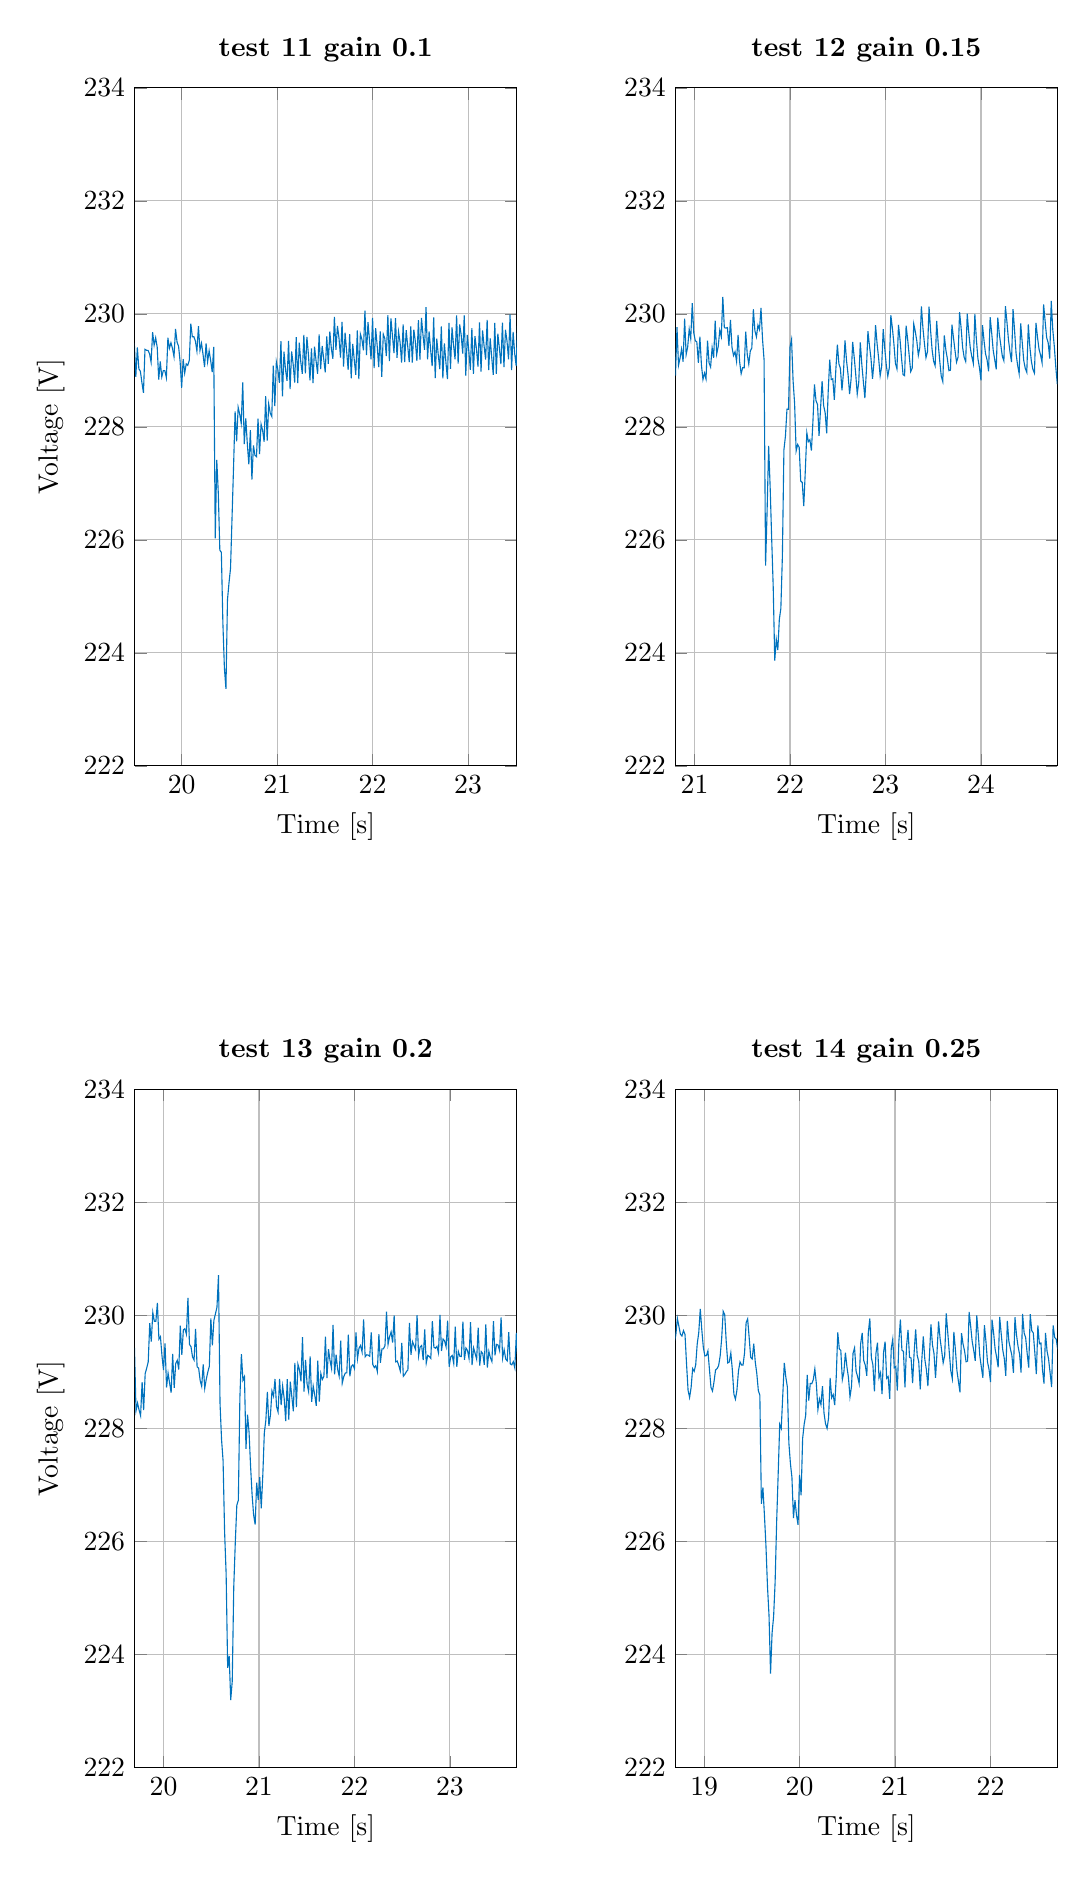
\begin{tikzpicture}

\begin{axis}[%
width=0.4\textwidth,
height=3.39in,
at={(1.297in,5.802in)},
scale only axis,
xmin=19.51,
xmax=23.51,
xlabel={Time [s]},
xmajorgrids,
ymin=222,
ymax=234,
ylabel={Voltage [V]},
ymajorgrids,
axis background/.style={fill=white},
title style={font=\bfseries},
title={test 11 gain 0.1}
]
\addplot [color=mycolor1,solid,forget plot]
  table[row sep=crcr]{%
19.504	229.488322012544\\
19.52	228.886831101655\\
19.536	229.407072096319\\
19.552	229.027828852114\\
19.568	228.983207865966\\
19.584	228.781163644479\\
19.6	228.60400102699\\
19.616	229.371613371668\\
19.632	229.355560651905\\
19.648	229.353564377921\\
19.664	229.293130874731\\
19.68	229.1438925588\\
19.696	229.67609564491\\
19.712	229.445969292431\\
19.728	229.575787808337\\
19.744	229.409090008157\\
19.76	228.838873157655\\
19.776	229.156995163178\\
19.792	228.884689740067\\
19.808	228.995807969809\\
19.824	228.995187071133\\
19.84	228.871897180971\\
19.856	229.576873363912\\
19.872	229.392906879379\\
19.888	229.488695098222\\
19.904	229.389525747135\\
19.92	229.24123109918\\
19.936	229.734390259675\\
19.952	229.500959984878\\
19.968	229.424935289295\\
19.984	229.15437357336\\
20	228.692907984684\\
20.016	229.20041032766\\
20.032	228.952333179939\\
20.048	229.114728036059\\
20.064	229.089672619557\\
20.08	229.177437269794\\
20.096	229.82625521812\\
20.112	229.594893141072\\
20.128	229.597533432729\\
20.144	229.517203831768\\
20.16	229.342181090907\\
20.176	229.781191650706\\
20.192	229.353286417014\\
20.208	229.479194469117\\
20.224	229.28309634014\\
20.24	229.058862088113\\
20.256	229.478401425993\\
20.272	229.153397223386\\
20.288	229.346375887397\\
20.304	229.175680027837\\
20.32	228.968113996125\\
20.336	229.416358947826\\
20.352	226.026408539162\\
20.368	227.415292992161\\
20.384	226.824147664588\\
20.4	225.816560813206\\
20.416	225.779475133607\\
20.432	224.525641695194\\
20.448	223.7252180766\\
20.464	223.364765085574\\
20.48	224.9372734363\\
20.496	225.238679165189\\
20.512	225.495491036295\\
20.528	226.400355998597\\
20.544	227.307136185878\\
20.56	228.276023381396\\
20.576	227.744751566148\\
20.592	228.346498901479\\
20.608	228.224920230965\\
20.624	228.064081885726\\
20.64	228.785647018233\\
20.656	227.694699842239\\
20.672	228.147894361462\\
20.688	227.694393086729\\
20.704	227.335105295168\\
20.72	227.942006539794\\
20.736	227.067720874282\\
20.752	227.672460982196\\
20.768	227.496891694368\\
20.784	227.473447992058\\
20.8	228.14689285341\\
20.816	227.519873582955\\
20.832	228.048084625806\\
20.848	227.94019920417\\
20.864	227.737227778476\\
20.88	228.542490905319\\
20.896	227.758861820412\\
20.912	228.405565333313\\
20.928	228.242923217836\\
20.944	228.185045026892\\
20.96	229.083353633055\\
20.976	228.368387809511\\
20.992	229.152207806959\\
21.008	229.010277860129\\
21.024	228.779111918401\\
21.04	229.517131546111\\
21.056	228.538630684516\\
21.072	229.332063633026\\
21.088	229.011591300431\\
21.104	228.815345784449\\
21.12	229.520489479022\\
21.136	228.670050035168\\
21.152	229.333707787017\\
21.168	229.111497551335\\
21.184	228.78476431347\\
21.2	229.587496697356\\
21.216	228.774903571906\\
21.232	229.491292938616\\
21.248	229.148711642475\\
21.264	228.937313763522\\
21.28	229.626611500855\\
21.296	228.945757496032\\
21.312	229.591191395082\\
21.328	229.280629842641\\
21.344	228.823445460804\\
21.36	229.391024224914\\
21.376	228.77364935003\\
21.392	229.419899087393\\
21.408	229.166854050782\\
21.424	228.938921430183\\
21.44	229.634943752356\\
21.456	229.023172880483\\
21.472	229.432199732535\\
21.488	229.207367124736\\
21.504	228.965575036658\\
21.52	229.600154439647\\
21.536	229.11645732455\\
21.552	229.687356963109\\
21.568	229.384878990342\\
21.584	229.205681366804\\
21.6	229.948492325871\\
21.616	229.362070765008\\
21.632	229.786207080516\\
21.648	229.575148793284\\
21.664	229.226356922867\\
21.68	229.859792028346\\
21.696	229.066587264235\\
21.712	229.668113703591\\
21.728	229.340490758216\\
21.744	229.010226227955\\
21.76	229.642617793009\\
21.776	228.8609704201\\
21.792	229.470263686495\\
21.808	229.18664028852\\
21.824	228.919096232312\\
21.84	229.705692419309\\
21.856	228.8472025303\\
21.872	229.642773111874\\
21.888	229.549892249701\\
21.904	229.35554034374\\
21.92	230.058342840556\\
21.936	229.269286754578\\
21.952	229.853890159529\\
21.968	229.52140852741\\
21.984	229.195862898805\\
22	229.93081797076\\
22.016	229.03996078878\\
22.032	229.745509002559\\
22.048	229.440144946764\\
22.064	229.056386602193\\
22.08	229.690943128232\\
22.096	228.883859200887\\
22.112	229.639581905326\\
22.128	229.563701481086\\
22.144	229.252194712152\\
22.16	229.976714037047\\
22.176	229.163642439313\\
22.192	229.92041694264\\
22.208	229.614985832349\\
22.224	229.305630825265\\
22.24	229.925328204731\\
22.256	229.222866173133\\
22.272	229.68265320133\\
22.288	229.495430812508\\
22.304	229.136847438844\\
22.32	229.813266941785\\
22.336	229.146245606421\\
22.352	229.710246031561\\
22.368	229.42671518247\\
22.384	229.145234444003\\
22.4	229.778612007988\\
22.416	229.136410588524\\
22.432	229.72186913334\\
22.448	229.505897854096\\
22.464	229.167971029164\\
22.48	229.890175837258\\
22.496	229.188770885732\\
22.512	229.930119943972\\
22.528	229.623973130089\\
22.544	229.363740728538\\
22.56	230.119595879508\\
22.576	229.195655560507\\
22.592	229.6874803919\\
22.608	229.364938040792\\
22.624	229.073970705083\\
22.64	229.937410649309\\
22.656	228.864612604654\\
22.672	229.562439039968\\
22.688	229.274133178134\\
22.704	229.020789847947\\
22.72	229.778729253522\\
22.736	228.858877467107\\
22.752	229.478829802873\\
22.768	229.14526235695\\
22.784	228.847338925118\\
22.8	229.839771620807\\
22.816	229.026129906035\\
22.832	229.760269960139\\
22.848	229.444201334642\\
22.864	229.193999991896\\
22.88	229.97374246171\\
22.896	229.119640286411\\
22.912	229.812451082772\\
22.928	229.627553559686\\
22.944	229.295173612394\\
22.96	229.975095063602\\
22.976	228.907044933188\\
22.992	229.626636886432\\
23.008	229.343023269192\\
23.024	229.01035881055\\
23.04	229.747411286768\\
23.056	228.939853529956\\
23.072	229.607159258631\\
23.088	229.380292365359\\
23.104	229.06589061536\\
23.12	229.847556451345\\
23.136	228.977345304537\\
23.152	229.707564840779\\
23.168	229.42801477845\\
23.184	229.191339982305\\
23.2	229.894516419399\\
23.216	229.006233034186\\
23.232	229.564861082647\\
23.248	229.22442840311\\
23.264	228.922123989396\\
23.28	229.840123342248\\
23.296	228.936289423338\\
23.312	229.648318330066\\
23.328	229.390970741754\\
23.344	229.110767139064\\
23.36	229.842550812357\\
23.376	229.057847131185\\
23.392	229.718244297569\\
23.408	229.517662460709\\
23.424	229.193953170941\\
23.44	229.989799744114\\
23.456	229.006568742042\\
23.472	229.681292789733\\
23.488	229.303155845235\\
23.504	229.077977107699\\
23.52	229.867167888703\\
};
\end{axis}

\begin{axis}[%
width=0.4\textwidth,
height=3.39in,
at={(4in,5.802in)},
scale only axis,
xmin=20.8,
xmax=24.8,
xlabel={Time [s]},
xmajorgrids,
ymin=222,
ymax=234,
ymajorgrids,
axis background/.style={fill=white},
title style={font=\bfseries},
title={test 12  gain 0.15}
]
\addplot [color=mycolor1,solid,forget plot]
  table[row sep=crcr]{%
20.8	228.906292313147\\
20.816	229.764410880001\\
20.832	229.090013021448\\
20.848	229.21393905652\\
20.864	229.375515317366\\
20.88	229.153096272057\\
20.896	229.913699294757\\
20.912	229.280870477069\\
20.928	229.412991543062\\
20.944	229.728683866886\\
20.96	229.560701881825\\
20.976	230.191079752055\\
20.992	229.661287120951\\
21.008	229.524983712198\\
21.024	229.50222301532\\
21.04	229.132856886867\\
21.056	229.595705382047\\
21.072	229.095601710286\\
21.088	228.839316307794\\
21.104	228.951787964361\\
21.12	228.847104456344\\
21.136	229.526428808429\\
21.152	229.133672391088\\
21.168	229.059122273992\\
21.184	229.401986894744\\
21.2	229.220795870906\\
21.216	229.879311320242\\
21.232	229.287701113456\\
21.248	229.424383286507\\
21.264	229.710144856526\\
21.28	229.596887960636\\
21.296	230.301070831415\\
21.312	229.755392330989\\
21.328	229.74938655061\\
21.344	229.756955202475\\
21.36	229.436229495991\\
21.376	229.894474317041\\
21.392	229.409486884237\\
21.408	229.262924441247\\
21.424	229.330885884681\\
21.44	229.157915161903\\
21.456	229.626347525265\\
21.472	229.154650398293\\
21.488	228.941434298703\\
21.504	229.046589545505\\
21.52	229.043852314807\\
21.536	229.685759100409\\
21.552	229.282962734205\\
21.568	229.110399776673\\
21.584	229.343610241702\\
21.6	229.39734216128\\
21.616	230.081297110658\\
21.632	229.703112067308\\
21.648	229.592882522184\\
21.664	229.800970400292\\
21.68	229.723074396076\\
21.696	230.103515722001\\
21.712	229.552264820876\\
21.728	229.189369826014\\
21.744	225.544710149575\\
21.76	226.51987917983\\
21.776	227.66130829854\\
21.792	226.925851268923\\
21.808	226.015502516153\\
21.824	225.162206696233\\
21.84	223.862833153024\\
21.856	224.240636694291\\
21.872	224.048130738893\\
21.888	224.594403490974\\
21.904	224.785388042899\\
21.92	225.712624177149\\
21.936	227.594396290871\\
21.952	227.835382357186\\
21.968	228.311604332543\\
21.984	228.310401528372\\
22	229.410932143077\\
22.016	229.545966312358\\
22.032	228.819060117133\\
22.048	228.413331265492\\
22.064	227.574266869752\\
22.08	227.68872575589\\
22.096	227.638042304254\\
22.112	227.041695298652\\
22.128	227.015453665092\\
22.144	226.597827051484\\
22.16	227.219036328151\\
22.176	227.894150011013\\
22.192	227.737824033292\\
22.208	227.773172504672\\
22.224	227.580465400492\\
22.24	228.09976199419\\
22.256	228.750622878505\\
22.272	228.463239303672\\
22.288	228.395812645567\\
22.304	227.840261678963\\
22.32	228.333480392334\\
22.336	228.807819164768\\
22.352	228.376058314065\\
22.368	228.249845859482\\
22.384	227.886565956222\\
22.4	228.631755689371\\
22.416	229.189579798614\\
22.432	228.837401023483\\
22.448	228.851963271949\\
22.464	228.477279190253\\
22.48	229.016460133017\\
22.496	229.457128110435\\
22.512	229.116464611886\\
22.528	229.031510986163\\
22.544	228.644764807532\\
22.56	228.970118931902\\
22.576	229.529643807041\\
22.592	229.167966221802\\
22.608	228.923749756898\\
22.624	228.579192625998\\
22.64	228.85422861868\\
22.656	229.504778468901\\
22.672	229.235743344683\\
22.688	228.934768087966\\
22.704	228.582797790207\\
22.72	228.79325604532\\
22.736	229.495471942966\\
22.752	229.105228095652\\
22.768	228.801942445737\\
22.784	228.509587225036\\
22.8	229.001717108408\\
22.816	229.692639682126\\
22.832	229.436788946358\\
22.848	229.211645974096\\
22.864	228.850165386698\\
22.88	229.153292750077\\
22.896	229.801983570435\\
22.912	229.472099681747\\
22.928	229.217018795692\\
22.944	228.903756876478\\
22.96	229.071457641675\\
22.976	229.729067656341\\
22.992	229.394963449969\\
23.008	229.09618172373\\
23.024	228.895512932627\\
23.04	229.048922547115\\
23.056	229.97537342566\\
23.072	229.750877345381\\
23.088	229.471496264857\\
23.104	229.124255927544\\
23.12	229.025388028756\\
23.136	229.806528120059\\
23.152	229.547804579846\\
23.168	229.215939713282\\
23.184	228.92400806824\\
23.2	228.905544158986\\
23.216	229.790951387819\\
23.232	229.55158442655\\
23.248	229.269702572228\\
23.264	228.977412288547\\
23.28	229.042466650827\\
23.296	229.822399066726\\
23.312	229.688212567995\\
23.328	229.519326160231\\
23.344	229.267260329157\\
23.36	229.409124033028\\
23.376	230.13200192733\\
23.392	229.752485483502\\
23.408	229.471234223255\\
23.424	229.22590276339\\
23.44	229.331939873512\\
23.456	230.126125430269\\
23.472	229.712929696125\\
23.488	229.366521036867\\
23.504	229.163082701233\\
23.52	229.080633158663\\
23.536	229.875028785507\\
23.552	229.477799277588\\
23.568	229.168311388248\\
23.584	228.897466359347\\
23.6	228.801455065418\\
23.616	229.61710329129\\
23.632	229.365359849867\\
23.648	229.205144272033\\
23.664	228.995332198985\\
23.68	229.003019004851\\
23.696	229.808899880726\\
23.712	229.578675496548\\
23.728	229.350540392337\\
23.744	229.144871971635\\
23.76	229.233698042724\\
23.776	230.031269068782\\
23.792	229.74946562087\\
23.808	229.40310699726\\
23.824	229.231155450323\\
23.84	229.156818454001\\
23.856	230.004083375388\\
23.872	229.670962802212\\
23.888	229.400083331924\\
23.904	229.244874118073\\
23.92	229.122685893875\\
23.936	229.997954021567\\
23.952	229.544034920042\\
23.968	229.210353685661\\
23.984	229.047333722605\\
24	228.824607800195\\
24.016	229.802125762676\\
24.032	229.526816406826\\
24.048	229.290597681694\\
24.064	229.186024361547\\
24.08	228.983825529026\\
24.096	229.94281114685\\
24.112	229.669323239991\\
24.128	229.355922403877\\
24.144	229.188103168088\\
24.16	229.019417135161\\
24.176	229.932451339055\\
24.192	229.645091148349\\
24.208	229.444485262228\\
24.224	229.245950808157\\
24.24	229.169455971502\\
24.256	230.136053837118\\
24.272	229.858180543494\\
24.288	229.541161451897\\
24.304	229.325203369722\\
24.32	229.148767323501\\
24.336	230.084178470652\\
24.352	229.70371690599\\
24.368	229.29289181051\\
24.384	229.088321155939\\
24.4	228.939633624411\\
24.416	229.832269814839\\
24.432	229.500182578303\\
24.448	229.173105397714\\
24.464	229.035797098771\\
24.48	228.965781049393\\
24.496	229.812283349268\\
24.512	229.417206268493\\
24.528	229.158786230954\\
24.544	229.017875231333\\
24.56	228.949815404299\\
24.576	229.840567415716\\
24.592	229.590275516277\\
24.608	229.37643366716\\
24.624	229.272593041991\\
24.64	229.136891528544\\
24.656	230.166979456362\\
24.672	229.868668918851\\
24.688	229.579218721139\\
24.704	229.488442029834\\
24.72	229.210564847842\\
24.736	230.230751699879\\
24.752	229.725157136675\\
24.768	229.427811753902\\
24.784	229.052419500151\\
24.8	228.751812770902\\
24.816	229.628152363245\\
};
\end{axis}

\begin{axis}[%
width=0.4\textwidth,
height=3.39in,
at={(1.297in,0.793in)},
scale only axis,
xmin=19.7,
xmax=23.7,
xlabel={Time [s]},
xmajorgrids,
ymin=222,
ymax=234,
ylabel={Voltage [V]},
ymajorgrids,
axis background/.style={fill=white},
title style={font=\bfseries},
title={test 13  gain 0.2}
]
\addplot [color=mycolor1,solid,forget plot]
  table[row sep=crcr]{%
19.696	229.431730370295\\
19.712	228.317804980386\\
19.728	228.453633147477\\
19.744	228.333261630427\\
19.76	228.230523791285\\
19.776	228.82552667518\\
19.792	228.330735343157\\
19.808	228.9748010204\\
19.824	229.071183658712\\
19.84	229.182946796767\\
19.856	229.867558408748\\
19.872	229.542055337054\\
19.888	230.055317078756\\
19.904	229.901109067394\\
19.92	229.899333796144\\
19.936	230.226107193235\\
19.952	229.584135761604\\
19.968	229.627603535374\\
19.984	229.291309831326\\
20	229.037375728199\\
20.016	229.510363030212\\
20.032	228.729535246025\\
20.048	228.982533481348\\
20.064	228.80669475992\\
20.08	228.636835558574\\
20.096	229.321843478525\\
20.112	228.721026735506\\
20.128	229.152530994684\\
20.144	229.210213275789\\
20.16	229.048261163004\\
20.176	229.823857593625\\
20.192	229.305242749976\\
20.208	229.749590928951\\
20.224	229.769108317876\\
20.24	229.67290374222\\
20.256	230.315160739583\\
20.272	229.490795576671\\
20.288	229.451431874753\\
20.304	229.269324666543\\
20.32	229.215034974578\\
20.336	229.765831123522\\
20.352	229.093837931506\\
20.368	229.072567203451\\
20.384	228.852262737651\\
20.4	228.750250693167\\
20.416	229.137963600061\\
20.432	228.713402843273\\
20.448	228.874866475788\\
20.464	229.00160775686\\
20.48	229.103445899137\\
20.496	229.950872465847\\
20.512	229.476633043274\\
20.528	229.919586005275\\
20.544	230.032067460547\\
20.56	230.149168097219\\
20.576	230.716555676845\\
20.592	228.450751677449\\
20.608	227.809713048065\\
20.624	227.432198906137\\
20.64	226.172870515\\
20.656	225.431365353753\\
20.672	223.768283994136\\
20.688	223.976339694608\\
20.704	223.198095809652\\
20.72	223.530951853147\\
20.736	225.202653640045\\
20.752	225.985498089561\\
20.768	226.646751537807\\
20.784	226.733575840376\\
20.8	228.542188256359\\
20.816	229.316853248992\\
20.832	228.85746874899\\
20.848	228.920614952232\\
20.864	227.64278378416\\
20.88	228.249017328347\\
20.896	227.942842845108\\
20.912	227.339136260484\\
20.928	226.828822644831\\
20.944	226.470898291657\\
20.96	226.304309239092\\
20.976	227.045757459679\\
20.992	226.738871634044\\
21.008	227.141186005348\\
21.024	226.591164402739\\
21.04	227.170452207652\\
21.056	227.926346721887\\
21.072	228.146957063155\\
21.088	228.649217027153\\
21.104	228.04811227281\\
21.12	228.238152394008\\
21.136	228.668769350093\\
21.152	228.576753615751\\
21.168	228.878393871195\\
21.184	228.391461249424\\
21.2	228.295730398379\\
21.216	228.878828376643\\
21.232	228.415905822044\\
21.248	228.75302636674\\
21.264	228.535311306754\\
21.28	228.135827067673\\
21.296	228.875199252156\\
21.312	228.158428502069\\
21.328	228.8315657961\\
21.344	228.566875259049\\
21.36	228.307261794609\\
21.376	229.16576936355\\
21.392	228.382384169898\\
21.408	229.140945116072\\
21.424	229.045072997761\\
21.44	228.836556457628\\
21.456	229.618921088418\\
21.472	228.657227322054\\
21.488	229.217858701144\\
21.504	228.788272043659\\
21.52	228.654594849944\\
21.536	229.279442383904\\
21.552	228.476694952798\\
21.568	228.754692495457\\
21.584	228.59834021316\\
21.6	228.405755835168\\
21.616	229.205218621421\\
21.632	228.477302155686\\
21.648	228.975706222445\\
21.664	228.871654217191\\
21.68	228.924293841265\\
21.696	229.627115869169\\
21.712	228.896689693478\\
21.728	229.407588985997\\
21.744	229.205713957977\\
21.76	229.06700171197\\
21.776	229.836261183777\\
21.792	228.95985205241\\
21.808	229.309096920785\\
21.824	229.047620748596\\
21.84	228.930134109145\\
21.856	229.55641533151\\
21.872	228.803279428393\\
21.888	228.919607359389\\
21.904	228.984507363861\\
21.92	228.989310214539\\
21.936	229.665021806876\\
21.952	228.928306970725\\
21.968	229.101586577591\\
21.984	229.130985781004\\
22	229.064025698874\\
22.016	229.702306858519\\
22.032	229.23775613688\\
22.048	229.425398136236\\
22.064	229.4724551012\\
22.08	229.355917317943\\
22.096	229.932499729125\\
22.112	229.272054781292\\
22.128	229.306993114751\\
22.144	229.302435613506\\
22.16	229.281905766339\\
22.176	229.70547159056\\
22.192	229.136689674956\\
22.208	229.080899416335\\
22.224	229.115385019408\\
22.24	229.01078114743\\
22.256	229.670999274771\\
22.272	229.167324459977\\
22.288	229.413335430136\\
22.304	229.412855343629\\
22.32	229.472424792609\\
22.336	230.069989283615\\
22.352	229.491141786253\\
22.368	229.629773670897\\
22.384	229.712543786398\\
22.4	229.522215600166\\
22.416	230.004489857002\\
22.432	229.183061223229\\
22.448	229.197514956286\\
22.464	229.121081294746\\
22.48	229.021020183491\\
22.496	229.51600242209\\
22.512	228.926597738856\\
22.528	228.960935825326\\
22.544	229.009575907214\\
22.56	229.040629876883\\
22.576	229.872201195597\\
22.592	229.308927266521\\
22.608	229.540360227799\\
22.624	229.471501070864\\
22.64	229.402624562691\\
22.656	230.009213900322\\
22.672	229.288574777533\\
22.688	229.446445095071\\
22.704	229.471735683411\\
22.72	229.214772140998\\
22.736	229.755230797825\\
22.752	229.160228698041\\
22.768	229.298399245161\\
22.784	229.277764553068\\
22.8	229.243272709019\\
22.816	229.904587363127\\
22.832	229.443877135378\\
22.848	229.423759267755\\
22.864	229.457122083956\\
22.88	229.341405010073\\
22.896	230.012751613309\\
22.912	229.375682903839\\
22.928	229.58614253484\\
22.944	229.55561829281\\
22.96	229.44789364098\\
22.976	229.911681983621\\
22.992	229.096512002876\\
23.008	229.269391703584\\
23.024	229.294704470627\\
23.04	229.152081178433\\
23.056	229.804376228244\\
23.072	229.096684617998\\
23.088	229.366845162699\\
23.104	229.281207340063\\
23.12	229.276287922509\\
23.136	229.895562204953\\
23.152	229.216642048498\\
23.168	229.427546423432\\
23.184	229.38565217453\\
23.2	229.243993250936\\
23.216	229.883504656531\\
23.232	229.125672159904\\
23.248	229.429910947472\\
23.264	229.331669003628\\
23.28	229.230616601729\\
23.296	229.786710697557\\
23.312	229.115214128224\\
23.328	229.363678984922\\
23.344	229.328686656366\\
23.36	229.131081707668\\
23.376	229.845635225458\\
23.392	229.080980851916\\
23.408	229.369074289791\\
23.424	229.25578310167\\
23.44	229.186858182348\\
23.456	229.902958116603\\
23.472	229.296793292327\\
23.488	229.492099265423\\
23.504	229.480084416026\\
23.52	229.382807509707\\
23.536	229.968192526458\\
23.552	229.250512954846\\
23.568	229.397269213068\\
23.584	229.234579374174\\
23.6	229.200104575786\\
23.616	229.706331255525\\
23.632	229.147069473989\\
23.648	229.129441542001\\
23.664	229.185503396976\\
23.68	229.076494324576\\
23.696	229.696343928951\\
23.712	229.150777183458\\
};
\end{axis}

\begin{axis}[%
width=0.4\textwidth,
height=3.39in,
at={(4in,0.793in)},
scale only axis,
xmin=18.7,
xmax=22.7,
xlabel={Time [s]},
xmajorgrids,
ymin=222,
ymax=234,
ymajorgrids,
axis background/.style={fill=white},
title style={font=\bfseries},
title={test 14  gain 0.25}
]
\addplot [color=mycolor1,solid,forget plot]
  table[row sep=crcr]{%
18.688	229.52121677921\\
18.704	229.658878986282\\
18.72	229.951307381085\\
18.736	229.81123796372\\
18.752	229.671470840253\\
18.768	229.640058911498\\
18.784	229.734881993623\\
18.8	229.669031898284\\
18.816	229.147938853702\\
18.832	228.681438286107\\
18.848	228.55214243192\\
18.864	228.729242010289\\
18.88	229.062685334798\\
18.896	229.014918919978\\
18.912	229.130175636505\\
18.928	229.501103872071\\
18.944	229.699494024478\\
18.96	230.120517777306\\
18.976	229.749166967757\\
18.992	229.437250195273\\
19.008	229.287569296019\\
19.024	229.292280903777\\
19.04	229.375518648934\\
19.056	229.050282671496\\
19.072	228.731785261785\\
19.088	228.666135844562\\
19.104	228.831559642615\\
19.12	229.039389814899\\
19.136	229.063309919599\\
19.152	229.116632377969\\
19.168	229.282837667942\\
19.184	229.594255147057\\
19.2	230.076358901324\\
19.216	230.017552377031\\
19.232	229.532245749169\\
19.248	229.163732197812\\
19.264	229.181219241493\\
19.28	229.340377264523\\
19.296	229.036223151414\\
19.312	228.61265388709\\
19.328	228.522300055906\\
19.344	228.684420276126\\
19.36	229.020596189775\\
19.376	229.180468099573\\
19.392	229.126239682825\\
19.408	229.126179344107\\
19.424	229.344283158866\\
19.44	229.875931517215\\
19.456	229.941530620498\\
19.472	229.615054962145\\
19.488	229.261593965985\\
19.504	229.233346735114\\
19.52	229.50465381478\\
19.536	229.179859814623\\
19.552	228.975799587389\\
19.568	228.675240907358\\
19.584	228.594485257768\\
19.6	226.670335047827\\
19.616	226.959808911499\\
19.632	226.468499933787\\
19.648	225.92366900851\\
19.664	225.206281709655\\
19.68	224.692310394286\\
19.696	223.666773581512\\
19.712	224.382411297243\\
19.728	224.674114447278\\
19.744	225.288244405887\\
19.76	226.35500074705\\
19.776	227.200281033166\\
19.792	228.074900505937\\
19.808	228.001807012444\\
19.824	228.588724738665\\
19.84	229.16533156776\\
19.856	228.911739698335\\
19.872	228.739377251003\\
19.888	227.747691645225\\
19.904	227.386343468033\\
19.92	227.137059533959\\
19.936	226.417709699855\\
19.952	226.73637944109\\
19.968	226.468972076529\\
19.984	226.298918455456\\
20	227.181044615202\\
20.016	226.819690394959\\
20.032	227.824803787015\\
20.048	228.075613469465\\
20.064	228.233487947567\\
20.08	228.951742544873\\
20.096	228.497605039577\\
20.112	228.800656656704\\
20.128	228.795995525711\\
20.144	228.868770122419\\
20.16	229.056949976262\\
20.176	228.790656732494\\
20.192	228.3378098379\\
20.208	228.526418172725\\
20.224	228.425109791177\\
20.24	228.75348607198\\
20.256	228.275020185181\\
20.272	228.085394543687\\
20.288	228.004849500758\\
20.304	228.191183575611\\
20.32	228.898179505402\\
20.336	228.547934590625\\
20.352	228.60496499825\\
20.368	228.416799265883\\
20.384	228.912588168659\\
20.4	229.703081245492\\
20.416	229.411603987827\\
20.432	229.382993857846\\
20.448	228.868008935891\\
20.464	228.996343972081\\
20.48	229.345723663782\\
20.496	229.097353925536\\
20.512	228.90491248905\\
20.528	228.561894359399\\
20.544	228.746947395211\\
20.56	229.334137924592\\
20.576	229.42996694376\\
20.592	229.017377984258\\
20.608	228.920309854132\\
20.624	228.798002658159\\
20.64	229.507569743555\\
20.656	229.695519412185\\
20.672	229.206082624999\\
20.688	229.124375150906\\
20.704	228.935264885158\\
20.72	229.701395473368\\
20.736	229.949424805043\\
20.752	229.254269881868\\
20.768	229.130894673961\\
20.784	228.660231560336\\
20.8	229.334086682679\\
20.816	229.523253639275\\
20.832	228.900450999241\\
20.848	228.989779519945\\
20.864	228.612872810198\\
20.88	229.354639203874\\
20.896	229.541303832438\\
20.912	228.89128728457\\
20.928	228.922284367847\\
20.944	228.529531951606\\
20.96	229.413216430424\\
20.976	229.583914034901\\
20.992	229.075548034558\\
21.008	229.100734818751\\
21.024	228.675417760303\\
21.04	229.541199935039\\
21.056	229.931682999142\\
21.072	229.389422308167\\
21.088	229.36766890469\\
21.104	228.73152759503\\
21.12	229.4512900984\\
21.136	229.746127890705\\
21.152	229.259473669009\\
21.168	229.25041341647\\
21.184	228.808770482343\\
21.2	229.348296504894\\
21.216	229.756195477018\\
21.232	229.29936777098\\
21.248	229.189607348047\\
21.264	228.697085984108\\
21.28	229.205972539592\\
21.296	229.630792501086\\
21.312	229.225828877307\\
21.328	229.047180251963\\
21.344	228.75544397204\\
21.36	229.276898047513\\
21.376	229.847071364834\\
21.392	229.481842073004\\
21.408	229.3315602833\\
21.424	228.899402266449\\
21.44	229.356615339951\\
21.456	229.898118088322\\
21.472	229.589547645901\\
21.488	229.386667757535\\
21.504	229.164783172356\\
21.52	229.294587079787\\
21.536	230.038927961639\\
21.552	229.705872473076\\
21.568	229.356020189645\\
21.584	229.022940248175\\
21.6	228.88358721495\\
21.616	229.71244324052\\
21.632	229.401123306864\\
21.648	229.031769195309\\
21.664	228.835379462051\\
21.68	228.644661796831\\
21.696	229.692206862418\\
21.712	229.501586321665\\
21.728	229.376979467706\\
21.744	229.184406954624\\
21.76	229.195967708109\\
21.776	230.065504191345\\
21.792	229.814751413133\\
21.808	229.543016550111\\
21.824	229.385507723589\\
21.84	229.201474311866\\
21.856	230.006569771619\\
21.872	229.663648498432\\
21.888	229.287676078439\\
21.904	229.089202128129\\
21.92	228.899050661398\\
21.936	229.831525074831\\
21.952	229.546685653574\\
21.968	229.184426240129\\
21.984	229.053724416481\\
22	228.82564694324\\
22.016	229.927740413356\\
22.032	229.703599496155\\
22.048	229.411892646991\\
22.064	229.266494625389\\
22.08	229.084641675759\\
22.096	229.976181096656\\
22.112	229.677303056008\\
22.128	229.395180029019\\
22.144	229.244821064458\\
22.16	228.933303724764\\
22.176	229.90806216188\\
22.192	229.550878250794\\
22.208	229.416752065139\\
22.224	229.293953033926\\
22.24	228.987728992066\\
22.256	229.971595251133\\
22.272	229.660561200021\\
22.288	229.459879265709\\
22.304	229.321093157782\\
22.32	228.993991227179\\
22.336	230.033002201487\\
22.352	229.694792034154\\
22.368	229.61259193998\\
22.384	229.330041970099\\
22.4	229.080914114\\
22.416	230.027822906354\\
22.432	229.734123016548\\
22.448	229.694644795548\\
22.464	229.345649104278\\
22.48	228.96588008303\\
22.496	229.827618777707\\
22.512	229.502802300455\\
22.528	229.517369950295\\
22.544	229.049337420078\\
22.56	228.79739414242\\
22.576	229.693563768185\\
22.592	229.373940667268\\
22.608	229.234659173803\\
22.624	228.992552560739\\
22.64	228.737391540672\\
22.656	229.82913668484\\
22.672	229.613696062965\\
22.688	229.583642190755\\
22.704	229.404910096932\\
};
\end{axis}
\end{tikzpicture}%
\caption{Step from 10 to 20 kW load, with various scaling factors.}
\label{fig:test11-14-10to20kwstepvolt}
\end{figure}

\begin{figure}[H]
\centering
% This file was created by matlab2tikz.
%
%The latest updates can be retrieved from
%  http://www.mathworks.com/matlabcentral/fileexchange/22022-matlab2tikz-matlab2tikz
%where you can also make suggestions and rate matlab2tikz.
%
\definecolor{mycolor1}{rgb}{0.00000,0.44700,0.74100}%
%
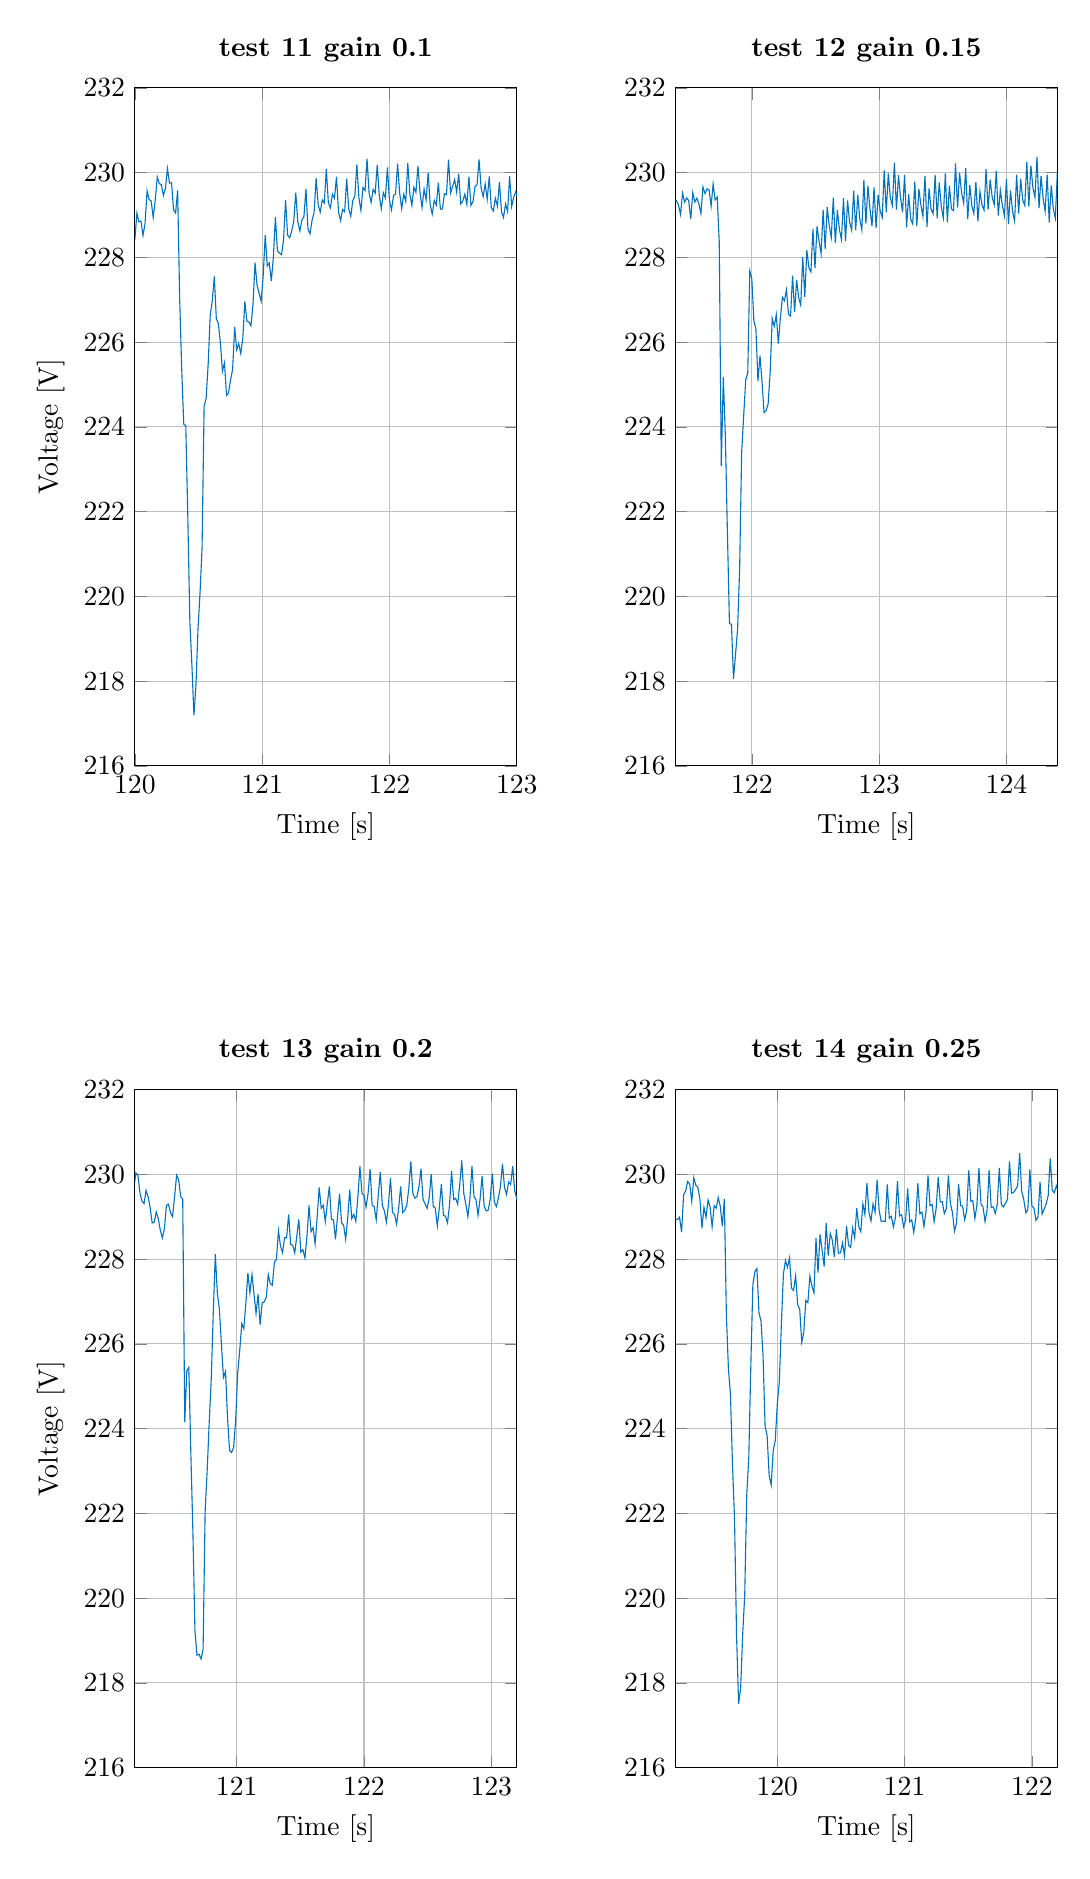
\begin{tikzpicture}

\begin{axis}[%
width=0.4\textwidth,
height=3.39in,
at={(1.297in,5.802in)},
scale only axis,
xmin=120,
xmax=123,
xlabel={Time [s]},
xmajorgrids,
ymin=216,
ymax=232,
ylabel={Voltage [V]},
ymajorgrids,
axis background/.style={fill=white},
title style={font=\bfseries},
title={test 11 gain 0.1}
]
\addplot [color=mycolor1,solid,forget plot]
  table[row sep=crcr]{%
120	228.418831902814\\
120.016	229.045491307679\\
120.032	228.839182483125\\
120.048	228.857699614523\\
120.064	228.518124681901\\
120.08	228.797969330697\\
120.096	229.570451921099\\
120.112	229.360337078303\\
120.128	229.335173477579\\
120.144	228.942589314625\\
120.16	229.34681711315\\
120.176	229.898606581838\\
120.192	229.739663959503\\
120.208	229.716296892719\\
120.224	229.460299708214\\
120.24	229.62884199592\\
120.256	230.096665525129\\
120.272	229.753259102104\\
120.288	229.761584424053\\
120.304	229.118604934431\\
120.32	229.048369033875\\
120.336	229.582821760923\\
120.352	227.019681435151\\
120.368	225.372564132742\\
120.384	224.065265257178\\
120.4	224.025919558114\\
120.416	221.88015059127\\
120.432	219.397138648559\\
120.448	218.387241319027\\
120.464	217.192985663592\\
120.48	217.900365133839\\
120.496	219.226083111155\\
120.512	220.081191937516\\
120.528	221.154192915387\\
120.544	224.488893042449\\
120.56	224.674156930744\\
120.576	225.488692842627\\
120.592	226.630263804574\\
120.608	226.974857248216\\
120.624	227.548224467057\\
120.64	226.554152544831\\
120.656	226.433638446234\\
120.672	225.985444012248\\
120.688	225.313686941987\\
120.704	225.513087691699\\
120.72	224.742504566836\\
120.736	224.804319426376\\
120.752	225.111159105595\\
120.768	225.358120118292\\
120.784	226.355811653736\\
120.8	225.821538368511\\
120.816	225.963733234217\\
120.832	225.730586221159\\
120.848	226.097318048344\\
120.864	226.958674737863\\
120.88	226.49220567632\\
120.896	226.47809932569\\
120.912	226.387808906801\\
120.928	226.89106664478\\
120.944	227.875719395223\\
120.96	227.341915892797\\
120.976	227.156182184363\\
120.992	226.964712198725\\
121.008	227.563998231008\\
121.024	228.522071979197\\
121.04	227.798576096055\\
121.056	227.868475658701\\
121.072	227.443403764351\\
121.088	228.001935261364\\
121.104	228.950230390356\\
121.12	228.155865796581\\
121.136	228.099763966941\\
121.152	228.064572197434\\
121.168	228.404584151029\\
121.184	229.350185257305\\
121.2	228.523829396018\\
121.216	228.461349519466\\
121.232	228.624776349257\\
121.248	228.848994478167\\
121.264	229.524630393854\\
121.28	228.838974708453\\
121.296	228.621266994052\\
121.312	228.882196269249\\
121.328	228.95846341897\\
121.344	229.609803367428\\
121.36	228.66841045154\\
121.376	228.554921664773\\
121.392	228.872240334353\\
121.408	229.060216343374\\
121.424	229.86794709192\\
121.44	229.24406717228\\
121.456	229.069528311643\\
121.472	229.354378388433\\
121.488	229.282818642101\\
121.504	230.086996956401\\
121.52	229.288519766675\\
121.536	229.168742693181\\
121.552	229.490715136958\\
121.568	229.396012464101\\
121.584	229.905663579334\\
121.6	229.064676157527\\
121.616	228.869092416391\\
121.632	229.128319727856\\
121.648	229.074369096373\\
121.664	229.854589479045\\
121.68	229.147175030013\\
121.696	228.968637688259\\
121.712	229.341447867492\\
121.728	229.444767163211\\
121.744	230.191172312973\\
121.76	229.402812038102\\
121.776	229.107829403505\\
121.792	229.647173046845\\
121.808	229.577324074177\\
121.824	230.326318027668\\
121.84	229.515158134079\\
121.856	229.29690193065\\
121.872	229.605194653778\\
121.888	229.51426959448\\
121.904	230.184347057713\\
121.92	229.457665955691\\
121.936	229.148358084186\\
121.952	229.527150289597\\
121.968	229.401696062135\\
121.984	230.120786383336\\
122	229.345628013024\\
122.016	229.119739229967\\
122.032	229.460724018463\\
122.048	229.495844766432\\
122.064	230.209320776896\\
122.08	229.525346651134\\
122.096	229.150165252509\\
122.112	229.490001803184\\
122.128	229.319940243127\\
122.144	230.220796202972\\
122.16	229.498832212766\\
122.176	229.226010439197\\
122.192	229.656795347426\\
122.208	229.53700026011\\
122.224	230.158382942643\\
122.24	229.533198251762\\
122.256	229.175429081544\\
122.272	229.61170414575\\
122.288	229.357154175445\\
122.304	229.999055405026\\
122.32	229.243069012368\\
122.336	229.018081182086\\
122.352	229.346333509617\\
122.368	229.233198813833\\
122.384	229.764140692619\\
122.4	229.136358568298\\
122.416	229.141988200348\\
122.432	229.504902407993\\
122.448	229.481869797061\\
122.464	230.303255925844\\
122.48	229.52041387437\\
122.496	229.672136838748\\
122.512	229.834573793193\\
122.528	229.538155401213\\
122.544	229.974359462432\\
122.56	229.262544317199\\
122.576	229.32808654622\\
122.592	229.494553742176\\
122.608	229.25080004489\\
122.624	229.902194756467\\
122.64	229.228003747724\\
122.656	229.312559139438\\
122.672	229.671005247066\\
122.688	229.715795481768\\
122.704	230.309296075824\\
122.72	229.639348761672\\
122.736	229.434333254842\\
122.752	229.728495028487\\
122.768	229.370219318626\\
122.784	229.911914570451\\
122.8	229.177491054716\\
122.816	229.09350134791\\
122.832	229.394910902725\\
122.848	229.211477597845\\
122.864	229.776177366769\\
122.88	229.079233173289\\
122.896	228.942307687443\\
122.912	229.260878289541\\
122.928	229.082902983837\\
122.944	229.925180536449\\
122.96	229.201543292138\\
122.976	229.427391388128\\
122.992	229.543577242375\\
123.008	229.403884758766\\
};
\end{axis}

\begin{axis}[%
width=0.4\textwidth,
height=3.39in,
at={(4in,5.802in)},
scale only axis,
xmin=121.4,
xmax=124.4,
xlabel={Time [s]},
xmajorgrids,
ymin=216,
ymax=232,
ymajorgrids,
axis background/.style={fill=white},
title style={font=\bfseries},
title={test 12  gain 0.15}
]
\addplot [color=mycolor1,solid,forget plot]
  table[row sep=crcr]{%
121.392	229.329233600182\\
121.408	229.336008804116\\
121.424	229.232031911473\\
121.44	229.014615107342\\
121.456	229.513822466712\\
121.472	229.30299772818\\
121.488	229.402207706769\\
121.504	229.341014459621\\
121.52	228.904659023208\\
121.536	229.525267545259\\
121.552	229.304764672634\\
121.568	229.397074240998\\
121.584	229.26455654544\\
121.6	229.034539365082\\
121.616	229.661487440321\\
121.632	229.505477140891\\
121.648	229.616590197539\\
121.664	229.59488685487\\
121.68	229.210119824861\\
121.696	229.730945668718\\
121.712	229.354076074153\\
121.728	229.423231445324\\
121.744	228.367947900745\\
121.76	223.077510892496\\
121.776	225.178092686521\\
121.792	223.780996847286\\
121.808	221.535260365712\\
121.824	219.36689574815\\
121.84	219.335615621271\\
121.856	218.054111159093\\
121.872	218.633549314088\\
121.888	219.223867515421\\
121.904	220.629372999634\\
121.92	223.392734808285\\
121.936	224.26605792687\\
121.952	225.110623983015\\
121.968	225.277882344736\\
121.984	227.680759150571\\
122	227.489555311431\\
122.016	226.504085775911\\
122.032	226.315187466334\\
122.048	225.077737834151\\
122.064	225.678053648557\\
122.08	225.062075896223\\
122.096	224.336235650558\\
122.112	224.385017031155\\
122.128	224.539957425427\\
122.144	225.294281710931\\
122.16	226.558428422156\\
122.176	226.372724289191\\
122.192	226.649223135401\\
122.208	225.967303966971\\
122.224	226.56316514631\\
122.24	227.059532686599\\
122.256	226.974676922292\\
122.272	227.234289342146\\
122.288	226.657298927585\\
122.304	226.614251619295\\
122.32	227.56596574582\\
122.336	226.714131618401\\
122.352	227.470539038686\\
122.368	227.047187522014\\
122.384	226.873548370547\\
122.4	228.00584278203\\
122.416	227.070675472865\\
122.432	228.171507326121\\
122.448	227.760152997559\\
122.464	227.656228076443\\
122.48	228.667329413847\\
122.496	227.745221747121\\
122.512	228.729715502744\\
122.528	228.385068039242\\
122.544	228.087898488525\\
122.56	229.123647367989\\
122.576	228.194819164993\\
122.592	229.183227713937\\
122.608	228.74545710343\\
122.624	228.466473245716\\
122.64	229.40935121403\\
122.656	228.339447093264\\
122.672	229.11507099288\\
122.688	228.653409320555\\
122.704	228.424377424731\\
122.72	229.398282772697\\
122.736	228.381778799208\\
122.752	229.345577138333\\
122.768	228.83051406644\\
122.784	228.64230537519\\
122.8	229.576362098478\\
122.816	228.641288807692\\
122.832	229.472944117616\\
122.848	228.902383535842\\
122.864	228.646496431612\\
122.88	229.827997339276\\
122.896	228.798533646342\\
122.912	229.69357678676\\
122.928	229.141534165302\\
122.944	228.740074067976\\
122.96	229.651742272664\\
122.976	228.694471838543\\
122.992	229.479459395602\\
123.008	229.098073273945\\
123.024	228.939570240117\\
123.04	230.054362656177\\
123.056	229.066376451912\\
123.072	229.980931568478\\
123.088	229.406843573087\\
123.104	229.22776844587\\
123.12	230.236216449234\\
123.136	229.127059887829\\
123.152	229.938592077913\\
123.168	229.413759514683\\
123.184	229.0657420392\\
123.2	229.947551805829\\
123.216	228.710783918253\\
123.232	229.492048316751\\
123.248	228.90259804292\\
123.264	228.78904919681\\
123.28	229.787520305149\\
123.296	228.739602584093\\
123.312	229.614139815733\\
123.328	229.235571638537\\
123.344	228.971674588358\\
123.36	229.925441845249\\
123.376	228.722557388479\\
123.392	229.625087489018\\
123.408	229.136710239682\\
123.424	229.030579567553\\
123.44	229.945215865149\\
123.456	228.918961983534\\
123.472	229.767520161586\\
123.488	229.204580947656\\
123.504	228.93039040135\\
123.52	229.980152261863\\
123.536	228.829069932199\\
123.552	229.687094886843\\
123.568	229.145141136763\\
123.584	229.104858717109\\
123.6	230.215140953345\\
123.616	229.176499357634\\
123.632	229.995916126759\\
123.648	229.518723855861\\
123.664	229.280524687076\\
123.68	230.103654125251\\
123.696	228.900886113972\\
123.712	229.702260739201\\
123.728	229.218674446383\\
123.744	229.036190944791\\
123.76	229.782952474683\\
123.776	228.849978870187\\
123.792	229.554138382569\\
123.808	229.23538908504\\
123.824	229.1153618085\\
123.84	230.083148260007\\
123.856	229.125308356573\\
123.872	229.837262929056\\
123.888	229.425014793728\\
123.904	229.241310432816\\
123.92	230.03672029924\\
123.936	228.983332833111\\
123.952	229.585924044012\\
123.968	229.221194037885\\
123.984	228.98186148554\\
124	229.844838127671\\
124.016	228.785749783893\\
124.032	229.578392900028\\
124.048	229.08788385774\\
124.064	228.855978156234\\
124.08	229.949539029198\\
124.096	229.03291450994\\
124.112	229.849173496609\\
124.128	229.352672058565\\
124.144	229.22271095608\\
124.16	230.25112485983\\
124.176	229.198492875194\\
124.192	230.164258704318\\
124.208	229.640005575378\\
124.224	229.41787255917\\
124.24	230.371234634185\\
124.256	229.161190577602\\
124.272	229.921059395313\\
124.288	229.392122250276\\
124.304	229.092483161194\\
124.32	229.953080965327\\
124.336	228.82733860477\\
124.352	229.699355630501\\
124.368	229.149522362908\\
124.384	228.924271590605\\
124.4	229.997645890483\\
124.416	229.111260644255\\
};
\end{axis}

\begin{axis}[%
width=0.4\textwidth,
height=3.39in,
at={(1.297in,0.793in)},
scale only axis,
xmin=120.2,
xmax=123.2,
xlabel={Time [s]},
xmajorgrids,
ymin=216,
ymax=232,
ylabel={Voltage [V]},
ymajorgrids,
axis background/.style={fill=white},
title style={font=\bfseries},
title={test 13  gain 0.2}
]
\addplot [color=mycolor1,solid,forget plot]
  table[row sep=crcr]{%
120.192	229.676825125908\\
120.208	230.034566776913\\
120.224	229.979779319795\\
120.24	229.563798855325\\
120.256	229.372559528866\\
120.272	229.312217368845\\
120.288	229.621685117139\\
120.304	229.472975560234\\
120.32	229.221489676028\\
120.336	228.854810963125\\
120.352	228.871390076256\\
120.368	229.116241608062\\
120.384	228.954981715402\\
120.4	228.680347320785\\
120.416	228.502065806712\\
120.432	228.717588699355\\
120.448	229.268574718022\\
120.464	229.298629493119\\
120.48	229.097520375222\\
120.496	229.004040683966\\
120.512	229.470399481516\\
120.528	229.97961504546\\
120.544	229.872676155102\\
120.56	229.47974243905\\
120.576	229.414309776685\\
120.592	224.154841122567\\
120.608	225.358551166955\\
120.624	225.447661004764\\
120.64	223.401843481296\\
120.656	221.55308393684\\
120.672	219.225325953597\\
120.688	218.656442162444\\
120.704	218.677270318581\\
120.72	218.566410784512\\
120.736	218.789257070679\\
120.752	222.043006992636\\
120.768	223.005533683734\\
120.784	224.145174959248\\
120.8	225.157281285458\\
120.816	226.735609767386\\
120.832	228.117894993098\\
120.848	227.200769122095\\
120.864	226.815914966219\\
120.88	225.999190216524\\
120.896	225.210685450094\\
120.912	225.354621884417\\
120.928	224.254331015699\\
120.944	223.482756009607\\
120.96	223.438563975963\\
120.976	223.561833435256\\
120.992	224.208323502642\\
121.008	225.325772679811\\
121.024	225.852908812898\\
121.04	226.482102971969\\
121.056	226.361258031864\\
121.072	226.967819501986\\
121.088	227.671968401246\\
121.104	227.208967460358\\
121.12	227.636847003585\\
121.136	227.174062780004\\
121.152	226.719482016779\\
121.168	227.172178138006\\
121.184	226.452600639208\\
121.2	226.970220322032\\
121.216	226.992759462624\\
121.232	227.091131065007\\
121.248	227.637119582491\\
121.264	227.425442263281\\
121.28	227.384523125426\\
121.296	227.929827975647\\
121.312	227.988953111842\\
121.328	228.671303895822\\
121.344	228.310088867808\\
121.36	228.1542800463\\
121.376	228.505719403771\\
121.392	228.504983404698\\
121.408	229.056336312062\\
121.424	228.347600377983\\
121.44	228.328480201942\\
121.456	228.147085070097\\
121.472	228.545977943818\\
121.488	228.939734415302\\
121.504	228.164679668692\\
121.52	228.22419952003\\
121.536	228.02943081603\\
121.552	228.545119515231\\
121.568	229.267239721493\\
121.584	228.652857558499\\
121.6	228.743453661924\\
121.616	228.359104794726\\
121.632	228.984751559205\\
121.648	229.691929716747\\
121.664	229.202291608582\\
121.68	229.271253489374\\
121.696	228.891139434551\\
121.712	229.315228565305\\
121.728	229.717095792579\\
121.744	228.945495892293\\
121.76	228.92774125532\\
121.776	228.470941735\\
121.792	229.003862184059\\
121.808	229.538221879204\\
121.824	228.853137162835\\
121.84	228.80053808\\
121.856	228.471740494449\\
121.872	228.966504730935\\
121.888	229.6388356625\\
121.904	228.95517808783\\
121.92	229.059218776602\\
121.936	228.892242294095\\
121.952	229.470448282156\\
121.968	230.191950023143\\
121.984	229.55437797269\\
122	229.503397233473\\
122.016	229.231243779477\\
122.032	229.546574880538\\
122.048	230.126926710015\\
122.064	229.271771494036\\
122.08	229.240099488541\\
122.096	228.928367261242\\
122.112	229.501632427503\\
122.128	230.054470453764\\
122.144	229.264524501028\\
122.16	229.14187115433\\
122.176	228.872679865518\\
122.192	229.283700660785\\
122.208	229.913775717103\\
122.224	229.104657730425\\
122.24	229.058407741726\\
122.256	228.828027646118\\
122.272	229.184113371887\\
122.288	229.714242238872\\
122.304	229.10102103107\\
122.32	229.151417957073\\
122.336	229.273499236412\\
122.352	229.669941518303\\
122.368	230.309301185711\\
122.384	229.541162505914\\
122.4	229.439955816191\\
122.416	229.479288727574\\
122.432	229.711863437359\\
122.448	230.135189840303\\
122.464	229.408000094648\\
122.48	229.301894912384\\
122.496	229.200395987533\\
122.512	229.440112456126\\
122.528	230.008677992921\\
122.544	229.248185677151\\
122.56	229.202680352201\\
122.576	228.781889055982\\
122.592	229.22109599756\\
122.608	229.770719550721\\
122.624	229.033773341371\\
122.64	229.015841707556\\
122.656	228.860607745901\\
122.672	229.282588481383\\
122.688	230.074078535184\\
122.704	229.405897326108\\
122.72	229.435660745407\\
122.736	229.295216595745\\
122.752	229.757711243501\\
122.768	230.331165890293\\
122.784	229.550011530565\\
122.8	229.296734593649\\
122.816	229.003534194214\\
122.832	229.428522897741\\
122.848	230.19407802323\\
122.864	229.48193265653\\
122.88	229.397504549223\\
122.896	229.035961648551\\
122.912	229.428119595976\\
122.928	229.965240850492\\
122.944	229.24896753726\\
122.96	229.138762148034\\
122.976	229.156919184899\\
122.992	229.4250519324\\
123.008	230.018000164477\\
123.024	229.342634324417\\
123.04	229.242505008098\\
123.056	229.444250089355\\
123.072	229.717340630715\\
123.088	230.246756904677\\
123.104	229.686667308938\\
123.12	229.527754758929\\
123.136	229.823915325114\\
123.152	229.762360327567\\
123.168	230.19448183463\\
123.184	229.610043160703\\
123.2	229.426013339442\\
123.216	229.62822211939\\
};
\end{axis}

\begin{axis}[%
width=0.4\textwidth,
height=3.39in,
at={(4in,0.793in)},
scale only axis,
xmin=119.2,
xmax=122.2,
xlabel={Time [s]},
xmajorgrids,
ymin=216,
ymax=232,
ymajorgrids,
axis background/.style={fill=white},
title style={font=\bfseries},
title={test 14  gain 0.25}
]
\addplot [color=mycolor1,solid,forget plot]
  table[row sep=crcr]{%
119.2	228.951240882303\\
119.216	228.933751531943\\
119.232	228.989337083538\\
119.248	228.637396549715\\
119.264	229.521840994611\\
119.28	229.609641727804\\
119.296	229.834653923324\\
119.312	229.771104568747\\
119.328	229.360505813166\\
119.344	229.92221254525\\
119.36	229.74481702238\\
119.376	229.697263065437\\
119.392	229.420285143248\\
119.408	228.736125564325\\
119.424	229.220604719838\\
119.44	228.987093295581\\
119.456	229.397200478228\\
119.472	229.230519179549\\
119.488	228.767224325825\\
119.504	229.259581451602\\
119.52	229.204297075213\\
119.536	229.45313960461\\
119.552	229.24582105339\\
119.568	228.780245872566\\
119.584	229.416977221726\\
119.6	226.690469631044\\
119.616	225.411890093469\\
119.632	224.818512687604\\
119.648	223.141712109839\\
119.664	221.882271696862\\
119.68	219.114832928545\\
119.696	217.507122450591\\
119.712	217.864768381916\\
119.728	219.141460881209\\
119.744	220.06296797251\\
119.76	222.429026927594\\
119.776	223.316332868285\\
119.792	225.480202811451\\
119.808	227.393760473719\\
119.824	227.705453564161\\
119.84	227.775599256808\\
119.856	226.73606240097\\
119.872	226.542381127534\\
119.888	225.731877742778\\
119.904	224.054737409994\\
119.92	223.840853345515\\
119.936	222.894112886239\\
119.952	222.672772393337\\
119.968	223.483985474074\\
119.984	223.717880975736\\
120	224.58317921979\\
120.016	225.114279755886\\
120.032	226.467606152471\\
120.048	227.649068023798\\
120.064	227.965141246696\\
120.08	227.806314016763\\
120.096	228.026590979224\\
120.112	227.317091878142\\
120.128	227.262478247683\\
120.144	227.61015664919\\
120.16	226.929313437525\\
120.176	226.819121856948\\
120.192	226.039539544923\\
120.208	226.276502148331\\
120.224	227.027489752922\\
120.24	226.973536294324\\
120.256	227.599065654505\\
120.272	227.3641637307\\
120.288	227.207095271706\\
120.304	228.495003310604\\
120.32	227.680602970226\\
120.336	228.584867235183\\
120.352	228.212851805907\\
120.368	227.828053460559\\
120.384	228.849756936389\\
120.4	228.082367737434\\
120.416	228.608484849395\\
120.432	228.452216561254\\
120.448	228.053633243655\\
120.464	228.708214317009\\
120.48	228.138454315378\\
120.496	228.148578995823\\
120.512	228.382115244152\\
120.528	228.081725965849\\
120.544	228.782117174201\\
120.56	228.327362423494\\
120.576	228.278211717553\\
120.592	228.734933153456\\
120.608	228.50507278616\\
120.624	229.203395823218\\
120.64	228.770787711452\\
120.656	228.649102578101\\
120.672	229.305437510366\\
120.688	229.055275199478\\
120.704	229.795701536288\\
120.72	229.103552049593\\
120.736	228.902239286527\\
120.752	229.304134610757\\
120.768	229.107554530693\\
120.784	229.869976669517\\
120.8	229.153608803753\\
120.816	228.892718893098\\
120.832	228.898062622413\\
120.848	228.891032031051\\
120.864	229.767022661589\\
120.88	228.964546309056\\
120.896	229.009651338356\\
120.912	228.759336610595\\
120.928	228.979165949238\\
120.944	229.840225863362\\
120.96	229.021675893648\\
120.976	229.052973864495\\
120.992	228.764342417237\\
121.008	228.917009494109\\
121.024	229.669339550464\\
121.04	228.882355146638\\
121.056	228.926684794177\\
121.072	228.63310722326\\
121.088	228.968116428177\\
121.104	229.793359325973\\
121.12	229.070736248778\\
121.136	229.111498764339\\
121.152	228.777083688049\\
121.168	229.116282271833\\
121.184	229.974525776393\\
121.2	229.260855337495\\
121.216	229.293344837307\\
121.232	228.886005812817\\
121.248	229.202596148161\\
121.264	229.942808842519\\
121.28	229.350316870478\\
121.296	229.354391374634\\
121.312	229.074565459752\\
121.328	229.195192072496\\
121.344	229.977395251386\\
121.36	229.307926496241\\
121.376	229.099010897465\\
121.392	228.662545930483\\
121.408	228.856205747919\\
121.424	229.7713363748\\
121.44	229.268769801611\\
121.456	229.247721456624\\
121.472	228.928438140564\\
121.488	229.156535718144\\
121.504	230.095885602857\\
121.52	229.366783738366\\
121.536	229.378696114341\\
121.552	228.961395486766\\
121.568	229.269713603866\\
121.584	230.148520331671\\
121.6	229.303229509396\\
121.616	229.229165418456\\
121.632	228.888556076104\\
121.648	229.162302781049\\
121.664	230.103658937653\\
121.68	229.219557383607\\
121.696	229.234669313323\\
121.712	229.078303418463\\
121.728	229.289714749353\\
121.744	230.153492570612\\
121.76	229.289707305751\\
121.776	229.232383009825\\
121.792	229.315939765322\\
121.808	229.407642153456\\
121.824	230.30942495922\\
121.84	229.558319847071\\
121.856	229.575537534468\\
121.872	229.641743900041\\
121.888	229.733881535287\\
121.904	230.504488980107\\
121.92	229.603301371927\\
121.936	229.407127120093\\
121.952	229.096643883607\\
121.968	229.166999936849\\
121.984	230.118367405772\\
122	229.258697090382\\
122.016	229.204394415644\\
122.032	228.915750077898\\
122.048	228.996976890985\\
122.064	229.824062076852\\
122.08	229.06161503585\\
122.096	229.176460808818\\
122.112	229.304374311579\\
122.128	229.500310907118\\
122.144	230.375409295631\\
122.16	229.624312098934\\
122.176	229.570435915268\\
122.192	229.731041205295\\
122.208	229.581670741158\\
};
\end{axis}
\end{tikzpicture}%
\caption{Step from 10 to 30 kW load, with various scaling factors.}
\label{fig:test11-14-10to30kwstepvolt}
\end{figure}

\begin{figure}[H]
\centering
% This file was created by matlab2tikz.
%
%The latest updates can be retrieved from
%  http://www.mathworks.com/matlabcentral/fileexchange/22022-matlab2tikz-matlab2tikz
%where you can also make suggestions and rate matlab2tikz.
%
\definecolor{mycolor1}{rgb}{0.00000,0.44700,0.74100}%
%
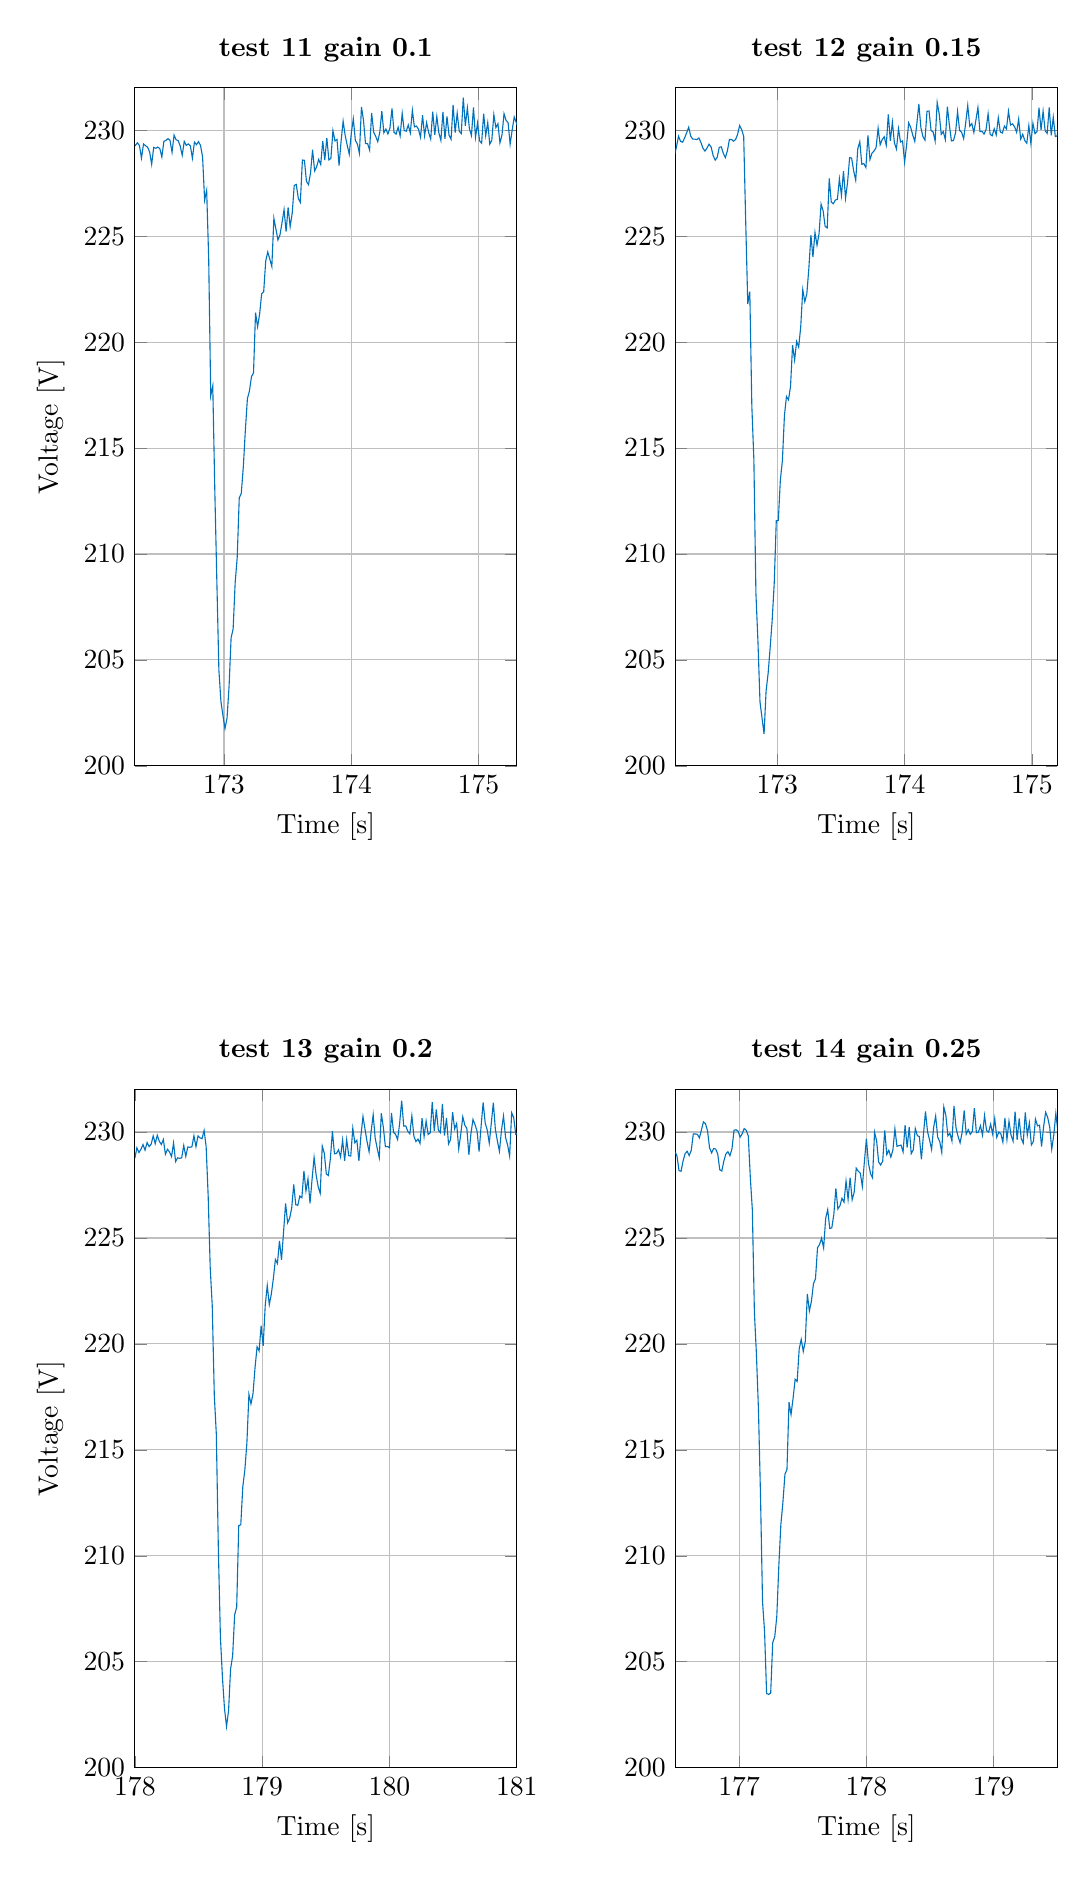
\begin{tikzpicture}

\begin{axis}[%
width=0.4\textwidth,
height=3.39in,
at={(1.297in,5.802in)},
scale only axis,
xmin=172.3,
xmax=175.3,
xlabel={Time [s]},
xmajorgrids,
ymin=200,
ymax=232,
ylabel={Voltage [V]},
ymajorgrids,
axis background/.style={fill=white},
title style={font=\bfseries},
title={test 11 gain 0.1}
]
\addplot [color=mycolor1,solid,forget plot]
  table[row sep=crcr]{%
172.288	229.363770878469\\
172.304	229.282151335247\\
172.32	229.408584861848\\
172.336	229.274744106882\\
172.352	228.685599631459\\
172.368	229.351924544723\\
172.384	229.270472182727\\
172.4	229.200732021126\\
172.416	228.973623415168\\
172.432	228.391029363415\\
172.448	229.191124124253\\
172.464	229.146885800155\\
172.48	229.206816120174\\
172.496	229.137603995378\\
172.512	228.7387328063\\
172.528	229.473701810898\\
172.544	229.523293276484\\
172.56	229.603271648426\\
172.576	229.527333321022\\
172.592	228.963331899432\\
172.608	229.770531283648\\
172.624	229.548282992712\\
172.64	229.513015200559\\
172.656	229.258684371694\\
172.672	228.819045015631\\
172.688	229.476230673908\\
172.704	229.287233608959\\
172.72	229.354808923975\\
172.736	229.265425012151\\
172.752	228.679377796388\\
172.768	229.44124859342\\
172.784	229.316438918283\\
172.8	229.464875659363\\
172.816	229.278211643587\\
172.832	228.741545376781\\
172.848	226.70243636262\\
172.864	227.166338342628\\
172.88	223.940473065044\\
172.896	217.470217842924\\
172.912	217.937500285017\\
172.928	213.01763762149\\
172.944	208.73499589527\\
172.96	204.526217500835\\
172.976	203.047232418536\\
172.992	202.371596161495\\
173.008	201.760336451302\\
173.024	202.250484152177\\
173.04	203.744334980633\\
173.056	206.041863404798\\
173.072	206.464723287532\\
173.088	208.651158027736\\
173.104	209.838539667461\\
173.12	212.643661920269\\
173.136	212.86304746088\\
173.152	214.11789158097\\
173.168	215.842652394795\\
173.184	217.328301527235\\
173.2	217.696224223078\\
173.216	218.368058119048\\
173.232	218.541351211241\\
173.248	221.395023883048\\
173.264	220.724668595315\\
173.28	221.322520768242\\
173.296	222.284256278637\\
173.312	222.382150750261\\
173.328	223.828163479882\\
173.344	224.255063153371\\
173.36	223.920004361153\\
173.376	223.566927592883\\
173.392	225.84463258074\\
173.408	225.34007931539\\
173.424	224.819999876613\\
173.44	225.063741701548\\
173.456	225.63387873904\\
173.472	226.254976389959\\
173.488	225.221981467491\\
173.504	226.360555169345\\
173.52	225.451378159069\\
173.536	226.082646527269\\
173.552	227.396646883556\\
173.568	227.445037959479\\
173.584	226.780586056189\\
173.6	226.594197463781\\
173.616	228.593844541134\\
173.632	228.580304257027\\
173.648	227.586409493891\\
173.664	227.43435254597\\
173.68	227.981663546598\\
173.696	229.080553981738\\
173.712	228.085548391339\\
173.728	228.275057985379\\
173.744	228.622895906687\\
173.76	228.382461409945\\
173.776	229.49132042219\\
173.792	228.588054484666\\
173.808	229.640390084592\\
173.824	228.598269668978\\
173.84	228.673368903114\\
173.856	229.981565670133\\
173.872	229.499242305525\\
173.888	229.563787181686\\
173.904	228.335612013469\\
173.92	229.479249793592\\
173.936	230.430394065677\\
173.952	229.757245802113\\
173.968	229.297837526702\\
173.984	228.870446565338\\
174	229.842356020379\\
174.016	230.543973502399\\
174.032	229.522782057988\\
174.048	229.351485930536\\
174.064	228.912979693686\\
174.08	231.102685228418\\
174.096	230.469563985605\\
174.112	229.368842583985\\
174.128	229.371747623747\\
174.144	229.063857193156\\
174.16	230.817762457846\\
174.176	229.910908581616\\
174.192	229.709220421805\\
174.208	229.460174557477\\
174.224	229.903512510622\\
174.24	230.905339631105\\
174.256	229.880606556472\\
174.272	230.055053884116\\
174.288	229.825341127838\\
174.304	230.10937849483\\
174.32	231.033750554885\\
174.336	229.900498752279\\
174.352	229.817730848726\\
174.368	230.143319550204\\
174.384	229.733608745715\\
174.4	230.799716258267\\
174.416	229.982458462769\\
174.432	229.955889331234\\
174.448	230.245934623175\\
174.464	229.873247703445\\
174.48	230.937541847305\\
174.496	230.157460761806\\
174.512	230.198670177074\\
174.528	230.048776800546\\
174.544	229.666883837008\\
174.56	230.70613096406\\
174.576	229.743282149975\\
174.592	230.362069376464\\
174.608	229.887902145121\\
174.624	229.58288180197\\
174.64	230.873119152701\\
174.656	229.782970392573\\
174.672	230.654563702255\\
174.688	229.873882457011\\
174.704	229.52028850202\\
174.72	230.862426619445\\
174.736	229.589982210692\\
174.752	230.656551421975\\
174.768	229.765766253171\\
174.784	229.573977147775\\
174.8	231.200958357176\\
174.816	229.884182442475\\
174.832	230.809525937336\\
174.848	229.956839870521\\
174.864	229.845813014421\\
174.88	231.541508214931\\
174.896	230.212969171198\\
174.912	231.055590815555\\
174.928	230.071386219016\\
174.944	229.752100382583\\
174.96	231.083417221038\\
174.976	229.662994414834\\
174.992	230.345943145086\\
175.008	229.495643908367\\
175.024	229.389737893039\\
175.04	230.788020141502\\
175.056	229.741490037626\\
175.072	230.358057484561\\
175.088	229.342239802585\\
175.104	229.526488560102\\
175.12	230.736433449954\\
175.136	230.125640083876\\
175.152	230.308644022798\\
175.168	229.405969124857\\
175.184	229.775782984623\\
175.2	230.783527902326\\
175.216	230.465387673422\\
175.232	230.352908982056\\
175.248	229.340129152064\\
175.264	230.007073499964\\
175.28	230.629129448485\\
175.296	230.365596562301\\
175.312	230.081630355578\\
};
\end{axis}

\begin{axis}[%
width=0.4\textwidth,
height=3.39in,
at={(4in,5.802in)},
scale only axis,
xmin=172.2,
xmax=175.2,
xlabel={Time [s]},
xmajorgrids,
ymin=200,
ymax=232,
ymajorgrids,
axis background/.style={fill=white},
title style={font=\bfseries},
title={test 12  gain 0.15}
]
\addplot [color=mycolor1,solid,forget plot]
  table[row sep=crcr]{%
172.192	228.801812680495\\
172.208	229.221282962401\\
172.224	229.719572102984\\
172.24	229.477870334726\\
172.256	229.43547644179\\
172.272	229.636437631041\\
172.288	229.881859408569\\
172.304	230.142396855351\\
172.32	229.719353376694\\
172.336	229.580642459393\\
172.352	229.581756298559\\
172.368	229.558030184756\\
172.384	229.63596684973\\
172.4	229.423351019423\\
172.416	229.154604168773\\
172.432	229.015326263219\\
172.448	229.160780371742\\
172.464	229.339894975686\\
172.48	229.214059389008\\
172.496	228.804652320533\\
172.512	228.588023493036\\
172.528	228.723432338594\\
172.544	229.191899816232\\
172.56	229.217932489861\\
172.576	228.912686600847\\
172.592	228.705423916482\\
172.608	229.030819581521\\
172.624	229.567512524344\\
172.64	229.564353679632\\
172.656	229.482022964154\\
172.672	229.561519757952\\
172.688	229.802266325667\\
172.704	230.221748209866\\
172.72	230.032741286904\\
172.736	229.710876327365\\
172.752	225.655922118929\\
172.768	221.800478089354\\
172.784	222.376788950801\\
172.8	216.982094965\\
172.816	214.447034968233\\
172.832	208.152218375505\\
172.848	205.8714514292\\
172.864	203.024296040622\\
172.88	202.263443248036\\
172.896	201.504101070558\\
172.912	203.538720556064\\
172.928	204.369542642397\\
172.944	205.586659125479\\
172.96	206.89934866933\\
172.976	208.63807572841\\
172.992	211.570204695553\\
173.008	211.584676421879\\
173.024	213.48898319915\\
173.04	214.398153330925\\
173.056	216.531598041324\\
173.072	217.436190526843\\
173.088	217.274734056732\\
173.104	217.915605328504\\
173.12	219.859486881058\\
173.136	219.156107742565\\
173.152	220.034615375013\\
173.168	219.76431102921\\
173.184	220.720944115694\\
173.2	222.474863607322\\
173.216	221.904765967813\\
173.232	222.2782457502\\
173.248	223.486934716182\\
173.264	225.050266092743\\
173.28	224.010481190038\\
173.296	225.173948997474\\
173.312	224.572866657244\\
173.328	225.118769721732\\
173.344	226.510722969634\\
173.36	226.199619946653\\
173.376	225.454325276535\\
173.392	225.388337874474\\
173.408	227.72458565705\\
173.424	226.613838874659\\
173.44	226.529238595107\\
173.456	226.704468530348\\
173.472	226.740767050657\\
173.488	227.70738716736\\
173.504	226.920680147443\\
173.52	228.073735942931\\
173.536	226.788990738972\\
173.552	227.537541973456\\
173.568	228.708122134253\\
173.584	228.684936638133\\
173.6	228.071977524984\\
173.616	227.641687473896\\
173.632	229.121079757868\\
173.648	229.457945008693\\
173.664	228.392548626425\\
173.68	228.428190275796\\
173.696	228.240432708484\\
173.712	229.759065194174\\
173.728	228.615552888341\\
173.744	228.918156612611\\
173.76	229.024604804107\\
173.776	229.176789409229\\
173.792	230.102525764546\\
173.808	229.313066886008\\
173.824	229.562164011174\\
173.84	229.692126534189\\
173.856	229.287977138979\\
173.872	230.747884406181\\
173.888	229.495369532377\\
173.904	230.387230791002\\
173.92	229.400222707646\\
173.936	229.114111660558\\
173.952	230.067608397772\\
173.968	229.442666411135\\
173.984	229.494933271571\\
174	228.487528339788\\
174.016	229.306513639471\\
174.032	230.347175489124\\
174.048	230.134167049286\\
174.064	229.773551065596\\
174.08	229.47084243317\\
174.096	230.294541632466\\
174.112	231.237954843256\\
174.128	230.121349535876\\
174.144	229.700195356953\\
174.16	229.531781125698\\
174.176	230.892655252126\\
174.192	230.907425590467\\
174.208	229.979107709217\\
174.224	229.923690916614\\
174.24	229.489815140063\\
174.256	231.311871955368\\
174.272	230.769796555602\\
174.288	229.805753494313\\
174.304	229.93687059809\\
174.32	229.561051832308\\
174.336	231.115539214474\\
174.352	230.225367007238\\
174.368	229.495154414832\\
174.384	229.514939485129\\
174.4	229.870295014004\\
174.416	230.881674250283\\
174.432	229.992993798884\\
174.448	229.90390812737\\
174.464	229.600813755896\\
174.48	230.35246655033\\
174.496	231.172323718467\\
174.512	230.188538426022\\
174.528	230.316942662549\\
174.544	229.895551522885\\
174.56	230.474366592521\\
174.576	231.075290210274\\
174.592	229.940068347782\\
174.608	229.945401352275\\
174.624	229.81822186643\\
174.64	230.040427509915\\
174.656	230.778634503178\\
174.672	229.807644601486\\
174.688	229.736699833866\\
174.704	230.073297238964\\
174.72	229.783581029029\\
174.736	230.591995104354\\
174.752	229.918580553094\\
174.768	229.869365829928\\
174.784	230.198806162414\\
174.8	230.060939488834\\
174.816	230.900118038281\\
174.832	230.247454783045\\
174.848	230.300198931815\\
174.864	230.165765046742\\
174.88	229.900521319683\\
174.896	230.527451894459\\
174.912	229.579710128154\\
174.928	229.811740839592\\
174.944	229.514889213213\\
174.96	229.385557209629\\
174.976	230.21856674262\\
174.992	229.376981245252\\
175.008	230.332886412196\\
175.024	229.844414059118\\
175.04	229.938089231672\\
175.056	231.059956748097\\
175.072	230.011118356177\\
175.088	230.902567345344\\
175.104	229.975463873661\\
175.12	229.853080871852\\
175.136	231.073276525133\\
175.152	229.762383658681\\
175.168	230.617866686225\\
175.184	229.701326382163\\
175.2	229.741851681786\\
175.216	231.154002200449\\
};
\end{axis}

\begin{axis}[%
width=0.4\textwidth,
height=3.39in,
at={(1.297in,0.793in)},
scale only axis,
xmin=178,
xmax=181,
xlabel={Time [s]},
xmajorgrids,
ymin=200,
ymax=232,
ylabel={Voltage [V]},
ymajorgrids,
axis background/.style={fill=white},
title style={font=\bfseries},
title={test 13  gain 0.2}
]
\addplot [color=mycolor1,solid,forget plot]
  table[row sep=crcr]{%
178	228.762094948678\\
178.016	229.255832045655\\
178.032	229.033586607114\\
178.048	229.188218600755\\
178.064	229.408407984698\\
178.08	229.146421364221\\
178.096	229.50158880654\\
178.112	229.313629672211\\
178.128	229.422115509331\\
178.144	229.821672883743\\
178.16	229.450447998905\\
178.176	229.849027827076\\
178.192	229.568406653849\\
178.208	229.409081706365\\
178.224	229.648915947883\\
178.24	228.950584338331\\
178.256	229.185970840463\\
178.272	229.062872169679\\
178.288	228.84145698037\\
178.304	229.486785496921\\
178.32	228.60887272045\\
178.336	228.784626066299\\
178.352	228.759423107508\\
178.368	228.782006059275\\
178.384	229.36386497033\\
178.4	228.854156883704\\
178.416	229.298635010038\\
178.432	229.281196007346\\
178.448	229.299092802848\\
178.464	229.823911995709\\
178.48	229.308514037472\\
178.496	229.82142853131\\
178.512	229.726355496223\\
178.528	229.687845604808\\
178.544	230.073040920044\\
178.56	229.313055949982\\
178.576	226.96526753771\\
178.592	223.586518414507\\
178.608	221.79716376354\\
178.624	217.592261599141\\
178.64	215.730867471849\\
178.656	210.283180527994\\
178.672	206.172743254804\\
178.688	204.264074963069\\
178.704	202.798504537805\\
178.72	201.948727745505\\
178.736	202.679975514746\\
178.752	204.667141656572\\
178.768	205.270978629971\\
178.784	207.216209929778\\
178.8	207.588838205793\\
178.816	211.41867646799\\
178.832	211.466338698684\\
178.848	213.264416911526\\
178.864	214.051686026535\\
178.88	215.320098857099\\
178.896	217.616965308667\\
178.912	217.170877658216\\
178.928	217.640299980434\\
178.944	218.878191041424\\
178.96	219.861720151198\\
178.976	219.668840990713\\
178.992	220.855550987048\\
179.008	219.904996479408\\
179.024	221.809443061911\\
179.04	222.756728378264\\
179.056	221.851671159828\\
179.072	222.355026757922\\
179.088	223.089859509595\\
179.104	223.985138501369\\
179.12	223.792499197955\\
179.136	224.865135786095\\
179.152	223.971438944713\\
179.168	225.265193085049\\
179.184	226.635330305504\\
179.2	225.717774553974\\
179.216	225.935214136853\\
179.232	226.412679209227\\
179.248	227.523027696276\\
179.264	226.571544612257\\
179.28	226.541837282451\\
179.296	226.984087254417\\
179.312	226.896105670456\\
179.328	228.162282767039\\
179.344	227.220530605374\\
179.36	227.793023879273\\
179.376	226.637551063854\\
179.392	227.766359976245\\
179.408	228.803734696039\\
179.424	227.967669912182\\
179.44	227.421434320591\\
179.456	227.103664985849\\
179.472	229.332304968859\\
179.488	229.005149582099\\
179.504	228.026438530982\\
179.52	227.950157458524\\
179.536	228.758579628906\\
179.552	230.0359409258\\
179.568	228.970087273343\\
179.584	228.992913475637\\
179.6	229.160165245793\\
179.616	228.819283328049\\
179.632	229.627393651011\\
179.648	228.647570344751\\
179.664	229.648027297712\\
179.68	228.886022797169\\
179.696	228.866249022258\\
179.712	230.184659530611\\
179.728	229.491374577512\\
179.744	229.616238797155\\
179.76	228.640584274775\\
179.776	229.840293186917\\
179.792	230.733779887878\\
179.808	230.131959692485\\
179.824	229.555066876946\\
179.84	229.069707297703\\
179.856	230.022413584527\\
179.872	230.822486761501\\
179.888	229.707434784968\\
179.904	229.2219900043\\
179.92	228.780942207605\\
179.936	230.884200086494\\
179.952	230.219361208202\\
179.968	229.309258681826\\
179.984	229.318881808071\\
180	229.258943076893\\
180.016	230.898806888931\\
180.032	229.987811545667\\
180.048	229.893522017668\\
180.064	229.644037520987\\
180.08	230.410415563498\\
180.096	231.485298138907\\
180.112	230.286378664791\\
180.128	230.288388501766\\
180.144	230.035606853378\\
180.16	229.913699890444\\
180.176	230.76883477326\\
180.192	229.802179434539\\
180.208	229.551306693147\\
180.224	229.66598161425\\
180.24	229.460251161467\\
180.256	230.65314981247\\
180.272	229.786871082233\\
180.288	230.514925740718\\
180.304	229.883556531852\\
180.32	229.959781891054\\
180.336	231.409953204873\\
180.352	230.057133107949\\
180.368	231.062041159736\\
180.384	230.095354224376\\
180.4	229.971994325443\\
180.416	231.326376315142\\
180.432	229.829654687308\\
180.448	230.662286678945\\
180.464	229.438135557069\\
180.48	229.634839193663\\
180.496	230.940803895572\\
180.512	230.148945927125\\
180.528	230.407373825454\\
180.544	229.205834978215\\
180.56	229.890243470368\\
180.576	230.716032868417\\
180.592	230.329488009742\\
180.608	230.16890582601\\
180.624	228.925959915398\\
180.64	229.924959135574\\
180.656	230.591809109733\\
180.672	230.354423800193\\
180.688	230.042209099516\\
180.704	229.078805358978\\
180.72	230.282548012725\\
180.736	231.398950561341\\
180.752	230.42671326394\\
180.768	230.098423877603\\
180.784	229.479065129121\\
180.8	230.414410455928\\
180.816	231.38663705122\\
180.832	230.127139105151\\
180.848	229.577669404495\\
180.864	229.092785103201\\
180.88	230.093853648396\\
180.896	230.75839924808\\
180.912	229.737999335752\\
180.928	229.393758569054\\
180.944	228.864520538361\\
180.96	230.906380040106\\
180.976	230.691989975515\\
180.992	229.892269826036\\
181.008	229.944932404053\\
};
\end{axis}

\begin{axis}[%
width=0.4\textwidth,
height=3.39in,
at={(4in,0.793in)},
scale only axis,
xmin=176.5,
xmax=179.5,
xlabel={Time [s]},
xmajorgrids,
ymin=200,
ymax=232,
ymajorgrids,
axis background/.style={fill=white},
title style={font=\bfseries},
title={test 14  gain 0.25}
]
\addplot [color=mycolor1,solid,forget plot]
  table[row sep=crcr]{%
176.496	229.091895556277\\
176.512	228.861316639587\\
176.528	228.179533993924\\
176.544	228.148945122819\\
176.56	228.638841601187\\
176.576	228.985348211838\\
176.592	229.091419194266\\
176.608	228.889267475808\\
176.624	229.13184042431\\
176.64	229.907902277276\\
176.656	229.909536531371\\
176.672	229.892884936639\\
176.688	229.725897068596\\
176.704	230.098758924796\\
176.72	230.481502513963\\
176.736	230.392232138252\\
176.752	230.05605877847\\
176.768	229.250583887487\\
176.784	229.01774773449\\
176.8	229.222099639778\\
176.816	229.199914700198\\
176.832	228.962193909087\\
176.848	228.221889098326\\
176.864	228.161097763809\\
176.88	228.628311171209\\
176.896	228.965336505019\\
176.912	229.073411874785\\
176.928	228.882049363411\\
176.944	229.210508314522\\
176.96	230.081696202473\\
176.976	230.109768012285\\
176.992	230.037362247629\\
177.008	229.760492181485\\
177.024	229.918597094546\\
177.04	230.166621679863\\
177.056	230.083148393097\\
177.072	229.817782081465\\
177.088	227.864493831294\\
177.104	226.324738270371\\
177.12	221.509646472756\\
177.136	219.516810476124\\
177.152	216.904968379602\\
177.168	212.874102391877\\
177.184	207.836387293908\\
177.2	206.418251852613\\
177.216	203.498447959793\\
177.232	203.461811827115\\
177.248	203.512849819654\\
177.264	205.90189944902\\
177.28	206.184671762507\\
177.296	207.134146553154\\
177.312	209.52416102483\\
177.328	211.477839590062\\
177.344	212.515000214812\\
177.36	213.846663430753\\
177.376	214.076437460122\\
177.392	217.252933065155\\
177.408	216.670336732662\\
177.424	217.434796889747\\
177.44	218.326585372565\\
177.456	218.228934263344\\
177.472	219.762093381027\\
177.488	220.215332931107\\
177.504	219.647731592517\\
177.52	220.124779466004\\
177.536	222.356579705406\\
177.552	221.55310244179\\
177.568	222.013850888781\\
177.584	222.83626522221\\
177.6	223.07600956933\\
177.616	224.539511608538\\
177.632	224.696032805026\\
177.648	224.991307254733\\
177.664	224.528332900327\\
177.68	225.923998453628\\
177.696	226.340559631522\\
177.712	225.448300906485\\
177.728	225.476057961225\\
177.744	226.100225163553\\
177.76	227.34122434293\\
177.776	226.37162952915\\
177.792	226.519998506601\\
177.808	226.874054578515\\
177.824	226.688120797501\\
177.84	227.689189729928\\
177.856	226.823434856467\\
177.872	227.849398425751\\
177.888	226.802956477276\\
177.904	227.163255486451\\
177.92	228.297402851455\\
177.936	228.153168842336\\
177.952	228.060757314105\\
177.968	227.432475185554\\
177.984	228.589692701496\\
178	229.682650770711\\
178.016	228.529404160671\\
178.032	228.043307150812\\
178.048	227.840254658933\\
178.064	229.990827163226\\
178.08	229.590994165224\\
178.096	228.585076571915\\
178.112	228.442857057473\\
178.128	228.625708772418\\
178.144	230.08151237851\\
178.16	228.940233254171\\
178.176	229.13938855303\\
178.192	228.816708260158\\
178.208	229.146813602933\\
178.224	230.153189690476\\
178.24	229.328702383106\\
178.256	229.359830231185\\
178.272	229.385331560998\\
178.288	229.064547449874\\
178.304	230.322179566409\\
178.32	229.261783193759\\
178.336	230.238141325407\\
178.352	228.979811113322\\
178.368	229.155063308412\\
178.384	230.16386652539\\
178.4	229.833710051855\\
178.416	229.786988596937\\
178.432	228.712558130644\\
178.448	229.871438183451\\
178.464	230.976744166586\\
178.48	230.025458510665\\
178.496	229.629131555258\\
178.512	229.176925407587\\
178.528	230.216860647535\\
178.544	230.754985358827\\
178.56	229.756657213253\\
178.576	229.550726680634\\
178.592	229.039124152703\\
178.608	231.190075745078\\
178.624	230.793042584125\\
178.64	229.824770739873\\
178.656	229.940458343713\\
178.672	229.576349745489\\
178.688	231.234454515764\\
178.704	230.188409417319\\
178.72	229.796228575256\\
178.736	229.49127545361\\
178.752	229.98090143624\\
178.768	231.015596554601\\
178.784	229.898545584754\\
178.8	230.113842460773\\
178.816	229.891417431462\\
178.832	230.035594291302\\
178.848	231.132353851203\\
178.864	229.967680073812\\
178.88	229.995338970632\\
178.896	230.300913435785\\
178.912	229.851427085041\\
178.928	230.782014682905\\
178.944	230.06750307644\\
178.96	230.001184698515\\
178.976	230.373704021699\\
178.992	229.900349644472\\
179.008	230.637500804133\\
179.024	229.749399679253\\
179.04	229.996128177813\\
179.056	229.918682801883\\
179.072	229.5259413229\\
179.088	230.661682800641\\
179.104	229.646944759577\\
179.12	230.514460838818\\
179.136	229.862748957364\\
179.152	229.569893781281\\
179.168	230.965554295577\\
179.184	229.62800716669\\
179.2	230.643165326725\\
179.216	229.696297622795\\
179.232	229.476878547229\\
179.248	230.928248583649\\
179.264	229.852830144237\\
179.28	230.432267929323\\
179.296	229.395160345798\\
179.312	229.556014383585\\
179.328	230.611066074359\\
179.344	230.291828953843\\
179.36	230.323532276456\\
179.376	229.317110458547\\
179.392	230.255963133598\\
179.408	230.93297145781\\
179.424	230.690663875814\\
179.44	230.22847498617\\
179.456	229.18851682504\\
179.472	229.85965652551\\
179.488	230.879515034793\\
179.504	230.053131852966\\
};
\end{axis}
\end{tikzpicture}%
\caption{Step from 10 to 50 kW load, with various scaling factors.}
\label{fig:test11-14-10to50kwstepvolt}
\end{figure}

\begin{figure}[H]
\centering
% This file was created by matlab2tikz.
%
%The latest updates can be retrieved from
%  http://www.mathworks.com/matlabcentral/fileexchange/22022-matlab2tikz-matlab2tikz
%where you can also make suggestions and rate matlab2tikz.
%
\definecolor{mycolor1}{rgb}{0.00000,0.44700,0.74100}%
%
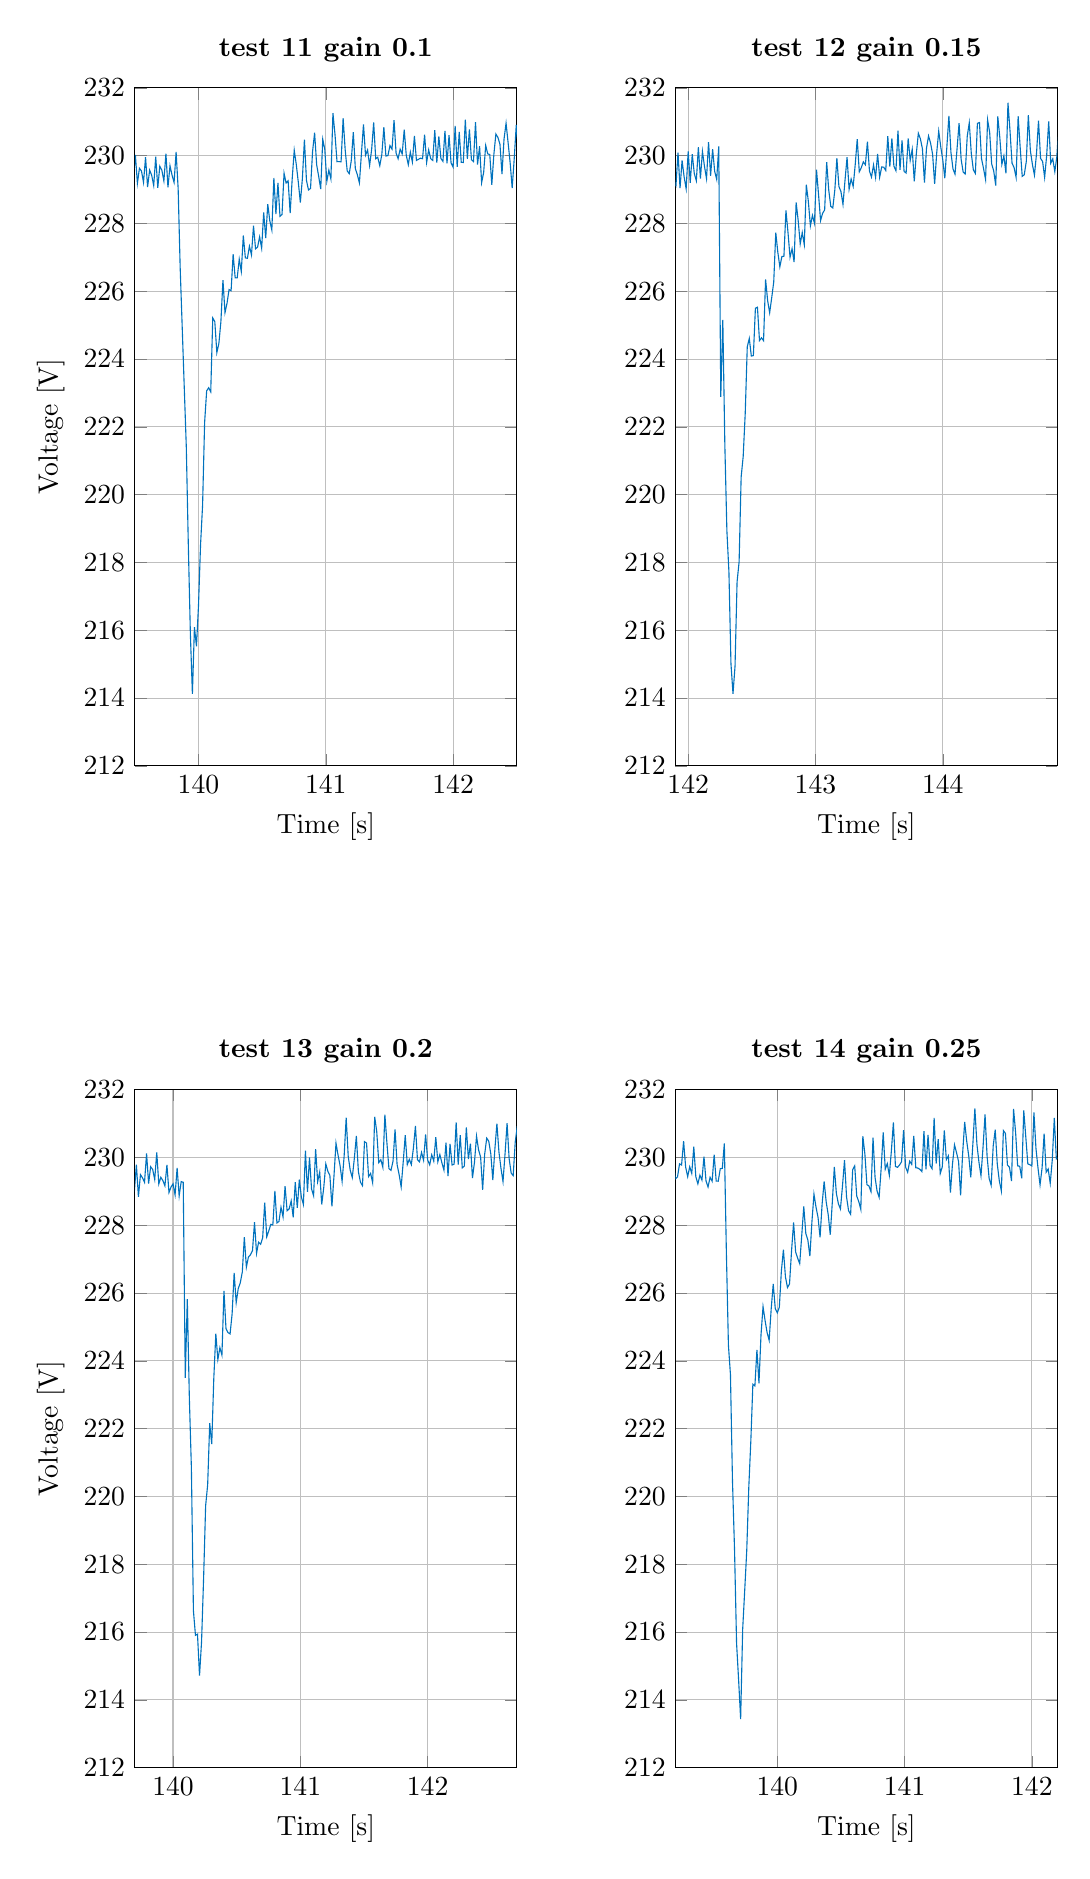
\begin{tikzpicture}

\begin{axis}[%
width=0.4\textwidth,
height=3.39in,
at={(1.297in,5.802in)},
scale only axis,
xmin=139.5,
xmax=142.5,
xlabel={Time [s]},
xmajorgrids,
ymin=212,
ymax=232,
ylabel={Voltage [V]},
ymajorgrids,
axis background/.style={fill=white},
title style={font=\bfseries},
title={test 11 gain 0.1}
]
\addplot [color=mycolor1,solid,forget plot]
  table[row sep=crcr]{%
139.488	229.312128752217\\
139.504	230.023956855111\\
139.52	229.184980743968\\
139.536	229.627982660848\\
139.552	229.546417642444\\
139.568	229.211717657766\\
139.584	229.958776523973\\
139.6	229.074690622709\\
139.616	229.572760608722\\
139.632	229.423701359346\\
139.648	229.121187343886\\
139.664	229.972296392313\\
139.68	229.049906992253\\
139.696	229.690010353776\\
139.712	229.572143425096\\
139.728	229.2558716688\\
139.744	230.058882854709\\
139.76	229.063565459736\\
139.776	229.702755238591\\
139.792	229.428191553186\\
139.808	229.211744033454\\
139.824	230.10780050095\\
139.84	229.034517567418\\
139.856	226.692582882624\\
139.872	224.935596861208\\
139.888	223.167143861331\\
139.904	221.420808990647\\
139.92	218.507763314004\\
139.936	215.904684439357\\
139.952	214.12174360206\\
139.968	216.092353430899\\
139.984	215.527184617901\\
140	216.738188498033\\
140.016	218.520780937423\\
140.032	219.685027397198\\
140.048	222.130873402752\\
140.064	223.063642105486\\
140.08	223.153357274437\\
140.096	223.03278312719\\
140.112	225.211655792207\\
140.128	225.104574506881\\
140.144	224.190243025013\\
140.16	224.46098796491\\
140.176	225.11259869086\\
140.192	226.33120601784\\
140.208	225.369332070032\\
140.224	225.646148966316\\
140.24	226.05100477982\\
140.256	226.017197846674\\
140.272	227.092421756866\\
140.288	226.398457836118\\
140.304	226.395512439889\\
140.32	226.944858319969\\
140.336	226.584104706591\\
140.352	227.643910571566\\
140.368	226.984554000397\\
140.384	226.973034467605\\
140.4	227.327836608043\\
140.416	227.07193241756\\
140.432	227.933252286961\\
140.448	227.251631590381\\
140.464	227.303804139863\\
140.48	227.606704462737\\
140.496	227.269566240934\\
140.512	228.32399431502\\
140.528	227.567538721028\\
140.544	228.56953164517\\
140.56	228.081200537605\\
140.576	227.80622781764\\
140.592	229.340510655416\\
140.608	228.279497651865\\
140.624	229.194446386922\\
140.64	228.211803381165\\
140.656	228.264294285541\\
140.672	229.482020205535\\
140.688	229.195881010153\\
140.704	229.25657098112\\
140.72	228.306520606255\\
140.736	229.315931350285\\
140.752	230.158997989308\\
140.768	229.739975826323\\
140.784	229.215545463105\\
140.8	228.619867594482\\
140.816	229.324190150291\\
140.832	230.474559751095\\
140.848	229.269964769645\\
140.864	228.989080283176\\
140.88	229.032669685582\\
140.896	230.125659327449\\
140.912	230.67567877654\\
140.928	229.736228520115\\
140.944	229.389033601253\\
140.96	229.014197068759\\
140.976	230.484482291283\\
140.992	230.183007586434\\
141.008	229.242721340239\\
141.024	229.572165354013\\
141.04	229.313824339065\\
141.056	231.257267241533\\
141.072	230.631366875627\\
141.088	229.822531008581\\
141.104	229.824679553546\\
141.12	229.818973207797\\
141.136	231.104911110134\\
141.152	230.182461092558\\
141.168	229.55238001688\\
141.184	229.468779856717\\
141.2	229.851962780087\\
141.216	230.69103767817\\
141.232	229.614325153226\\
141.248	229.434694538712\\
141.264	229.197211944195\\
141.28	230.076474041118\\
141.296	230.925181494148\\
141.312	230.013954884741\\
141.328	230.167173714639\\
141.344	229.70960745588\\
141.36	230.17865883184\\
141.376	230.97762026686\\
141.392	229.911230501752\\
141.408	229.953566380105\\
141.424	229.703804714713\\
141.44	230.034969166228\\
141.456	230.840124774389\\
141.472	229.989791685628\\
141.488	230.003896829527\\
141.504	230.296862150836\\
141.52	230.192411698391\\
141.536	231.046869075331\\
141.552	230.07559378347\\
141.568	229.91034841117\\
141.584	230.19269868946\\
141.6	230.047804471821\\
141.616	230.768616594106\\
141.632	230.010146982008\\
141.648	229.735302286665\\
141.664	230.102922436925\\
141.68	229.81370083322\\
141.696	230.580905919094\\
141.712	229.8599749259\\
141.728	229.893606834098\\
141.744	229.925838431046\\
141.76	229.909568871412\\
141.776	230.620592814663\\
141.792	229.798736924225\\
141.808	230.170720447545\\
141.824	229.913877266458\\
141.84	229.859700464679\\
141.856	230.749522902486\\
141.872	229.793881025201\\
141.888	230.569545264862\\
141.904	229.919669880662\\
141.92	229.831807064045\\
141.936	230.733867046837\\
141.952	229.771491258519\\
141.968	230.60304965993\\
141.984	229.7842529708\\
142	229.663721049397\\
142.016	230.878678290698\\
142.032	229.67063848485\\
142.048	230.70166689051\\
142.064	229.802379928294\\
142.08	229.799745133451\\
142.096	231.058973511655\\
142.112	229.906341481119\\
142.128	230.776566434445\\
142.144	229.881869418883\\
142.16	229.824681818445\\
142.176	230.988540288896\\
142.192	229.739210987605\\
142.208	230.277208211323\\
142.224	229.20614372536\\
142.24	229.503819215703\\
142.256	230.300486866656\\
142.272	230.052482427041\\
142.288	230.03284775973\\
142.304	229.142059820765\\
142.32	230.02984331269\\
142.336	230.636403001574\\
142.352	230.53902860734\\
142.368	230.336456603117\\
142.384	229.456933102734\\
142.4	230.489647376509\\
142.416	230.957522177538\\
142.432	230.384132098252\\
142.448	229.794570934711\\
142.464	229.043502997064\\
142.48	229.904207463161\\
142.496	230.903835286735\\
142.512	230.242106491944\\
};
\end{axis}

\begin{axis}[%
width=0.4\textwidth,
height=3.39in,
at={(4in,5.802in)},
scale only axis,
xmin=141.9,
xmax=144.9,
xlabel={Time [s]},
xmajorgrids,
ymin=212,
ymax=232,
ymajorgrids,
axis background/.style={fill=white},
title style={font=\bfseries},
title={test 12  gain 0.15}
]
\addplot [color=mycolor1,solid,forget plot]
  table[row sep=crcr]{%
141.888	229.266356944381\\
141.904	229.12105967501\\
141.92	230.092247573657\\
141.936	229.040666359992\\
141.952	229.862829240955\\
141.968	229.375135549264\\
141.984	229.022612767824\\
142	230.126056570873\\
142.016	229.201590716561\\
142.032	230.043624978155\\
142.048	229.470119427511\\
142.064	229.259780353815\\
142.08	230.250014909299\\
142.096	229.320413252674\\
142.112	230.125115105062\\
142.128	229.681369757792\\
142.144	229.321782953804\\
142.16	230.399669796222\\
142.176	229.408624884085\\
142.192	230.190355892674\\
142.208	229.541632031149\\
142.224	229.299554198153\\
142.24	230.275466466272\\
142.256	222.886455700567\\
142.272	225.157180902243\\
142.288	221.460474425888\\
142.304	218.935319534714\\
142.32	217.724304020194\\
142.336	215.012450018201\\
142.352	214.126414657809\\
142.368	214.940436768157\\
142.384	217.426372363015\\
142.4	218.018741524872\\
142.416	220.52005120608\\
142.432	221.126243709165\\
142.448	222.389874480357\\
142.464	224.361153264769\\
142.48	224.609148103304\\
142.496	224.088619892534\\
142.512	224.104029049304\\
142.528	225.498114629237\\
142.544	225.528493423337\\
142.56	224.545532590426\\
142.576	224.626960905112\\
142.592	224.543853440993\\
142.608	226.351094751549\\
142.624	225.729354707534\\
142.64	225.366777924915\\
142.656	225.805577716749\\
142.672	226.274728972167\\
142.688	227.73103721405\\
142.704	227.155720126235\\
142.72	226.7223069635\\
142.736	227.024808689636\\
142.752	227.031251031299\\
142.768	228.386792128681\\
142.784	227.736342171332\\
142.8	227.005996611695\\
142.816	227.255168281566\\
142.832	226.861009711691\\
142.848	228.621937707757\\
142.864	228.089619428154\\
142.88	227.397773184414\\
142.896	227.731588320689\\
142.912	227.375789155172\\
142.928	229.144036475428\\
142.944	228.647724386763\\
142.96	227.929560653544\\
142.976	228.238205580608\\
142.992	228.004377120041\\
143.008	229.585835293045\\
143.024	228.852341082386\\
143.04	228.08590887062\\
143.056	228.302482225375\\
143.072	228.399097543297\\
143.088	229.809453066823\\
143.104	228.988829346237\\
143.12	228.505247524205\\
143.136	228.456867526452\\
143.152	228.993550220997\\
143.168	229.925073375966\\
143.184	229.092335451125\\
143.2	228.941074503315\\
143.216	228.561899134354\\
143.232	229.274281392176\\
143.248	229.952786493513\\
143.264	229.009512887792\\
143.28	229.313222216895\\
143.296	229.094460608185\\
143.312	229.730192398676\\
143.328	230.489303297871\\
143.344	229.523730377553\\
143.36	229.647590392318\\
143.376	229.816589655799\\
143.392	229.73174574199\\
143.408	230.412103799746\\
143.424	229.550868181878\\
143.44	229.368965422919\\
143.456	229.727796784989\\
143.472	229.357371791957\\
143.488	230.051701306046\\
143.504	229.36265487161\\
143.52	229.667313416475\\
143.536	229.660833167159\\
143.552	229.563520164574\\
143.568	230.572203867361\\
143.584	229.67821465447\\
143.6	230.508395179242\\
143.616	229.690874348779\\
143.632	229.556168564439\\
143.648	230.737911822267\\
143.664	229.585486020886\\
143.68	230.448388064084\\
143.696	229.533748635089\\
143.712	229.487881449718\\
143.728	230.507606862002\\
143.744	229.860045166117\\
143.76	230.188573816454\\
143.776	229.242242133448\\
143.792	230.054060043413\\
143.808	230.661831662281\\
143.824	230.497532686253\\
143.84	230.204770857333\\
143.856	229.207013034065\\
143.872	230.215513935873\\
143.888	230.582328680232\\
143.904	230.373070755361\\
143.92	230.04313699306\\
143.936	229.166387285576\\
143.952	230.070611607334\\
143.968	230.725535876812\\
143.984	230.262072797193\\
144	229.870069650489\\
144.016	229.335592174863\\
144.032	230.260015079861\\
144.048	231.173772199396\\
144.064	230.099394946834\\
144.08	229.611675329632\\
144.096	229.454322511568\\
144.112	230.202282341085\\
144.128	230.960923053131\\
144.144	229.896166317122\\
144.16	229.516717443631\\
144.176	229.459297468727\\
144.192	230.570307978498\\
144.208	230.969742450436\\
144.224	230.060933650061\\
144.24	229.579516681724\\
144.256	229.475350925842\\
144.272	230.955199519732\\
144.288	230.975785767681\\
144.304	229.918397441996\\
144.32	229.622540744288\\
144.336	229.297809198581\\
144.352	231.055512530103\\
144.368	230.698577400488\\
144.384	229.756642589723\\
144.4	229.551256457022\\
144.416	229.119614432733\\
144.432	231.15851570124\\
144.448	230.532269960736\\
144.464	229.741482753281\\
144.48	229.993202804998\\
144.496	229.48101772163\\
144.512	231.560069481253\\
144.528	230.731792687968\\
144.544	229.778451778601\\
144.56	229.648814599298\\
144.576	229.360088023793\\
144.592	231.162214328789\\
144.608	230.238364740939\\
144.624	229.391487413384\\
144.64	229.436056531483\\
144.656	229.827915391728\\
144.672	231.196034189766\\
144.688	230.149254591927\\
144.704	229.742027177614\\
144.72	229.426804320307\\
144.736	230.046236017845\\
144.752	231.035037375603\\
144.768	229.918334452705\\
144.784	229.830096878813\\
144.8	229.35740605712\\
144.816	230.006579791301\\
144.832	231.012199717499\\
144.848	229.776671584819\\
144.864	229.908335550589\\
144.88	229.528859819128\\
144.896	229.974499593909\\
144.912	230.954795454634\\
};
\end{axis}

\begin{axis}[%
width=0.4\textwidth,
height=3.39in,
at={(1.297in,0.793in)},
scale only axis,
xmin=139.7,
xmax=142.7,
xlabel={Time [s]},
xmajorgrids,
ymin=212,
ymax=232,
ylabel={Voltage [V]},
ymajorgrids,
axis background/.style={fill=white},
title style={font=\bfseries},
title={test 13  gain 0.2}
]
\addplot [color=mycolor1,solid,forget plot]
  table[row sep=crcr]{%
139.696	228.992328528427\\
139.712	229.789897481612\\
139.728	228.842001328261\\
139.744	229.493471208429\\
139.76	229.400144578145\\
139.776	229.267871540465\\
139.792	230.120398859134\\
139.808	229.226471360701\\
139.824	229.726731088677\\
139.84	229.646259029781\\
139.856	229.350896406422\\
139.872	230.15024199986\\
139.888	229.218649978832\\
139.904	229.41489181195\\
139.92	229.31873937957\\
139.936	229.163329255583\\
139.952	229.782367510273\\
139.968	228.965410368759\\
139.984	229.125192898051\\
140	229.222702307914\\
140.016	228.895434997563\\
140.032	229.6908802231\\
140.048	228.864435979863\\
140.064	229.288040078971\\
140.08	229.268299823432\\
140.096	223.501164215497\\
140.112	225.818540308568\\
140.128	222.914916464099\\
140.144	220.854533734508\\
140.16	216.632930433108\\
140.176	215.905260113416\\
140.192	215.938870583423\\
140.208	214.714885597483\\
140.224	215.720581520639\\
140.24	217.588004330415\\
140.256	219.728735947652\\
140.272	220.349430308579\\
140.288	222.161790129492\\
140.304	221.542970062684\\
140.32	223.472913669518\\
140.336	224.801010084476\\
140.352	224.040710543911\\
140.368	224.389332848131\\
140.384	224.170846908479\\
140.4	226.064039049425\\
140.416	224.947012997988\\
140.432	224.833405674127\\
140.448	224.796136436822\\
140.464	225.386057348132\\
140.48	226.59438214451\\
140.496	225.717115679103\\
140.512	226.12754912009\\
140.528	226.302528053893\\
140.544	226.61914112073\\
140.56	227.64973401983\\
140.576	226.762868598793\\
140.592	227.061207314159\\
140.608	227.129185710004\\
140.624	227.247974053506\\
140.64	228.093447569351\\
140.656	227.174612017632\\
140.672	227.502244161936\\
140.688	227.44119766701\\
140.704	227.628574213949\\
140.72	228.67023261686\\
140.736	227.658807856976\\
140.752	227.833577132678\\
140.768	228.026856878767\\
140.784	228.008429973966\\
140.8	229.013354686653\\
140.816	228.069766443759\\
140.832	228.112367688002\\
140.848	228.533133169988\\
140.864	228.24735057018\\
140.88	229.155104829392\\
140.896	228.4274582775\\
140.912	228.482859478008\\
140.928	228.719836007206\\
140.944	228.233323442663\\
140.96	229.274927796011\\
140.976	228.513820517606\\
140.992	229.348383278772\\
141.008	228.833226009081\\
141.024	228.614880475626\\
141.04	230.198653645415\\
141.056	228.986872885694\\
141.072	229.999109033903\\
141.088	229.069242794058\\
141.104	228.873292461599\\
141.12	230.248167248708\\
141.136	229.285928980537\\
141.152	229.567352190911\\
141.168	228.61441493971\\
141.184	229.116339777432\\
141.2	229.810231654972\\
141.216	229.593153045825\\
141.232	229.468661930707\\
141.248	228.556860384829\\
141.264	229.441691893177\\
141.28	230.421379421894\\
141.296	230.073296228235\\
141.312	229.761644747459\\
141.328	229.296300861169\\
141.344	230.03848630122\\
141.36	231.172909698978\\
141.376	230.037156643807\\
141.392	229.620331905684\\
141.408	229.406632733231\\
141.424	229.969723058985\\
141.44	230.634424479422\\
141.456	229.577713427598\\
141.472	229.274432280909\\
141.488	229.169004961017\\
141.504	230.466676563549\\
141.52	230.423274502674\\
141.536	229.436127408823\\
141.552	229.530650197951\\
141.568	229.253500456494\\
141.584	231.199367084994\\
141.6	230.764567864931\\
141.616	229.847458128458\\
141.632	229.934416130873\\
141.648	229.711335754099\\
141.664	231.266134741844\\
141.68	230.433240663623\\
141.696	229.672154818712\\
141.712	229.619974202934\\
141.728	229.889232513011\\
141.744	230.825778652005\\
141.76	229.789163528972\\
141.776	229.494736434078\\
141.792	229.130716736386\\
141.808	229.864825627358\\
141.824	230.657259335347\\
141.84	229.790109091315\\
141.856	229.944257738064\\
141.872	229.789098493592\\
141.888	230.272029315693\\
141.904	230.928161957633\\
141.92	229.93515337799\\
141.936	229.872067183701\\
141.952	230.146613243989\\
141.968	229.917492103918\\
141.984	230.678775246657\\
142	229.927555384895\\
142.016	229.783670614713\\
142.032	230.079700559712\\
142.048	229.89514567646\\
142.064	230.600395517253\\
142.08	229.874809151768\\
142.096	230.084975192485\\
142.112	229.840946519884\\
142.128	229.627486478939\\
142.144	230.434247454548\\
142.16	229.453010095676\\
142.176	230.397894065207\\
142.192	229.776464888998\\
142.208	229.80454931342\\
142.224	231.036104619055\\
142.24	229.789154193124\\
142.256	230.655022304725\\
142.272	229.692883746095\\
142.288	229.746769229738\\
142.304	230.883730035651\\
142.32	229.9510770986\\
142.336	230.409257868465\\
142.352	229.391218156833\\
142.368	229.86336924325\\
142.384	230.62932031147\\
142.4	230.223921371829\\
142.416	230.014615917875\\
142.432	229.044143942228\\
142.448	230.094915868642\\
142.464	230.570695096753\\
142.48	230.478200505405\\
142.496	230.110209364357\\
142.512	229.335184719022\\
142.528	230.238129694086\\
142.544	230.999887905833\\
142.56	230.162953674641\\
142.576	229.679507658081\\
142.592	229.289429461495\\
142.608	230.108721299427\\
142.624	231.014246733474\\
142.64	229.972083555638\\
142.656	229.540757836836\\
142.672	229.464435144051\\
142.688	230.453958547891\\
142.704	230.919781846624\\
};
\end{axis}

\begin{axis}[%
width=0.4\textwidth,
height=3.39in,
at={(4in,0.793in)},
scale only axis,
xmin=139.2,
xmax=142.2,
xlabel={Time [s]},
xmajorgrids,
ymin=212,
ymax=232,
ymajorgrids,
axis background/.style={fill=white},
title style={font=\bfseries},
title={test 14  gain 0.25}
]
\addplot [color=mycolor1,solid,forget plot]
  table[row sep=crcr]{%
139.184	230.046659585997\\
139.2	229.370743556026\\
139.216	229.425091504339\\
139.232	229.811184618903\\
139.248	229.777318098631\\
139.264	230.483778829946\\
139.28	229.715954421862\\
139.296	229.434822638483\\
139.312	229.72578841353\\
139.328	229.529076468874\\
139.344	230.318417557997\\
139.36	229.431307724292\\
139.376	229.22104630379\\
139.392	229.475765965712\\
139.408	229.332589105091\\
139.424	230.026608213226\\
139.44	229.307416391965\\
139.456	229.129527119347\\
139.472	229.417522033238\\
139.488	229.298519243217\\
139.504	230.082492712797\\
139.52	229.305224037603\\
139.536	229.299548525003\\
139.552	229.667381779557\\
139.568	229.677032668082\\
139.584	230.417357373279\\
139.6	227.197669595641\\
139.616	224.466083464365\\
139.632	223.595854855431\\
139.648	220.446979615542\\
139.664	218.442823397233\\
139.68	215.678498397109\\
139.696	214.596467585024\\
139.712	213.435060247527\\
139.728	216.08055109406\\
139.744	217.22906562358\\
139.76	218.405246962629\\
139.776	220.262806432839\\
139.792	221.630169035576\\
139.808	223.31063936842\\
139.824	223.261059790364\\
139.84	224.326401378383\\
139.856	223.336833396236\\
139.872	224.766878825851\\
139.888	225.600593191984\\
139.904	225.19209668365\\
139.92	224.833234694898\\
139.936	224.608377822094\\
139.952	225.529529932738\\
139.968	226.266686916617\\
139.984	225.54378637474\\
140	225.416279164511\\
140.016	225.581629290373\\
140.032	226.650102394958\\
140.048	227.280691064061\\
140.064	226.476630737689\\
140.08	226.164451874475\\
140.096	226.270121741505\\
140.112	227.245142985236\\
140.128	228.082643449938\\
140.144	227.208226394342\\
140.16	227.026991171987\\
140.176	226.86864578652\\
140.192	227.698617199114\\
140.208	228.555958918769\\
140.224	227.757671408467\\
140.24	227.564426236384\\
140.256	227.089026159415\\
140.272	228.099976396447\\
140.288	228.918637663972\\
140.304	228.537572612307\\
140.32	228.234029158478\\
140.336	227.643135436234\\
140.352	228.622041250997\\
140.368	229.295870949189\\
140.384	228.690771583421\\
140.4	228.309984502021\\
140.416	227.721847598474\\
140.432	228.666307699442\\
140.448	229.722927158255\\
140.464	228.94019750225\\
140.48	228.633562912631\\
140.496	228.481058816565\\
140.512	229.153701842348\\
140.528	229.920018220412\\
140.544	228.834751123823\\
140.56	228.42743455212\\
140.576	228.322114127777\\
140.592	229.634587855805\\
140.608	229.75304501747\\
140.624	228.862380339206\\
140.64	228.69774114538\\
140.656	228.467961479894\\
140.672	230.627122070789\\
140.688	230.10412675414\\
140.704	229.198940697995\\
140.72	229.159911839983\\
140.736	228.990235185079\\
140.752	230.583176236307\\
140.768	229.410786640345\\
140.784	229.005688385713\\
140.8	228.824741934077\\
140.816	229.67674827841\\
140.832	230.736654476808\\
140.848	229.654877124151\\
140.864	229.818520930481\\
140.88	229.473926067274\\
140.896	230.186957177734\\
140.912	231.035894999592\\
140.928	229.735218055268\\
140.944	229.709370926605\\
140.96	229.776624186847\\
140.976	229.873614076609\\
140.992	230.805684335727\\
141.008	229.713518794689\\
141.024	229.563976177016\\
141.04	229.890465746862\\
141.056	229.796928984603\\
141.072	230.636556133668\\
141.088	229.696447495883\\
141.104	229.687968887637\\
141.12	229.649383257121\\
141.136	229.58274343467\\
141.152	230.779172617807\\
141.168	229.653048449796\\
141.184	230.667475539809\\
141.2	229.762463112636\\
141.216	229.669617744842\\
141.232	231.164260769112\\
141.248	229.823064328214\\
141.264	230.541325839741\\
141.28	229.525739313351\\
141.296	229.72347766572\\
141.312	230.795651217123\\
141.328	229.936530838512\\
141.344	230.04886653432\\
141.36	228.964029182034\\
141.376	229.801999451219\\
141.392	230.372602674646\\
141.408	230.141636101726\\
141.424	229.880916970637\\
141.44	228.881499606724\\
141.456	230.125859606032\\
141.472	231.04640668549\\
141.488	230.477671539565\\
141.504	230.038902853573\\
141.52	229.414264194516\\
141.536	230.374807863703\\
141.552	231.447244104049\\
141.568	230.396460446515\\
141.584	229.861466946639\\
141.6	229.461522955889\\
141.616	230.29604148314\\
141.632	231.269580451857\\
141.648	230.037785971051\\
141.664	229.383208391422\\
141.68	229.179543766782\\
141.696	230.338646991029\\
141.712	230.816702301524\\
141.728	229.808080739731\\
141.744	229.312247737274\\
141.76	229.016133418135\\
141.776	230.792963751387\\
141.792	230.710525014659\\
141.808	229.774814522088\\
141.824	229.710759924248\\
141.84	229.302357562393\\
141.856	231.431640036406\\
141.872	230.740012308109\\
141.888	229.751594542308\\
141.904	229.743055287198\\
141.92	229.38530095332\\
141.936	231.39037813112\\
141.952	230.606238287515\\
141.968	229.809278805592\\
141.984	229.786352733037\\
142	229.75087898669\\
142.016	231.327358449035\\
142.032	230.26393569136\\
142.048	229.687684975764\\
142.064	229.191091870868\\
142.08	229.692780195181\\
142.096	230.70557525759\\
142.112	229.566605039667\\
142.128	229.659115416516\\
142.144	229.237568320569\\
142.16	229.924420762227\\
142.176	231.164333949253\\
142.192	229.957768297863\\
142.208	230.004721821582\\
};
\end{axis}
\end{tikzpicture}%
\caption{Step from 30 to 50 kW load, with various scaling factors.}
\label{fig:test11-14-30to50kwstepvolt}
\end{figure}

\begin{figure}[H]
\centering
% This file was created by matlab2tikz.
%
%The latest updates can be retrieved from
%  http://www.mathworks.com/matlabcentral/fileexchange/22022-matlab2tikz-matlab2tikz
%where you can also make suggestions and rate matlab2tikz.
%
\definecolor{mycolor1}{rgb}{0.00000,0.44700,0.74100}%
%
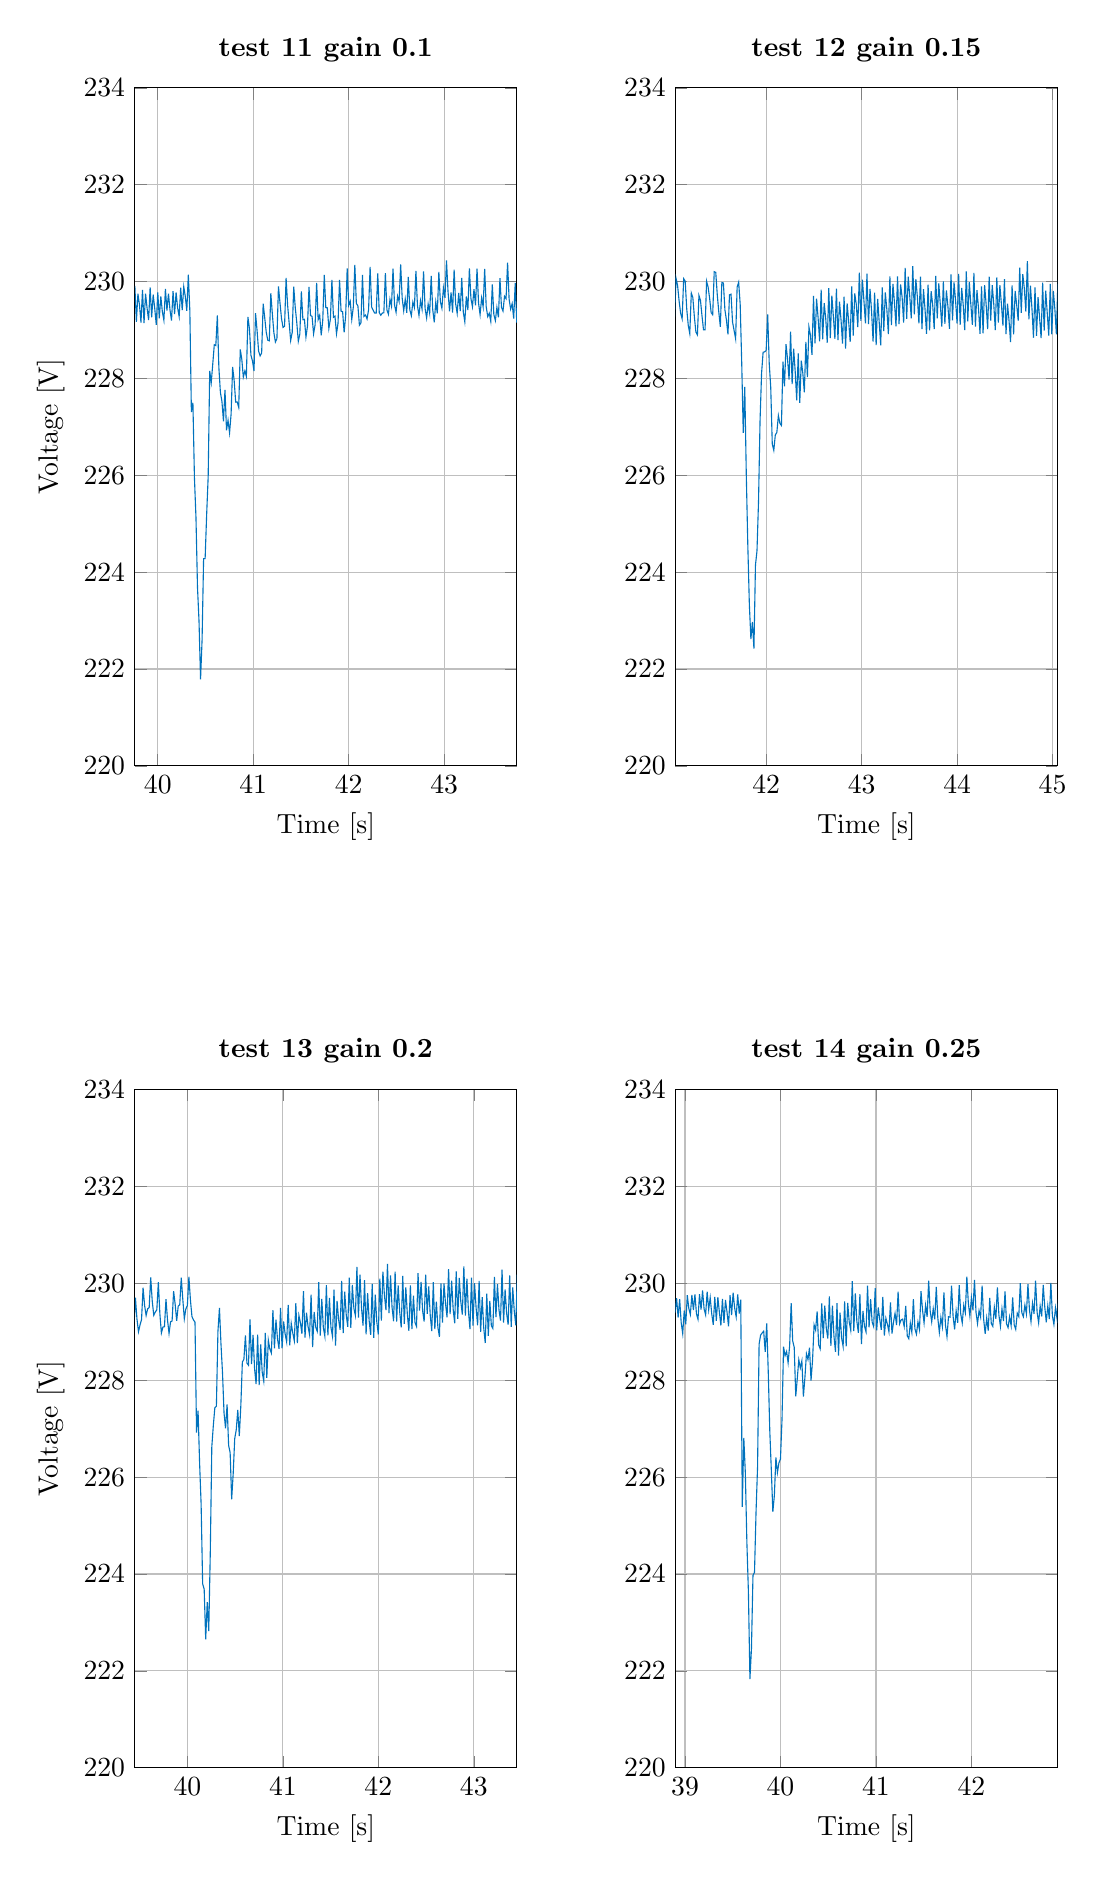
\begin{tikzpicture}

\begin{axis}[%
width=0.4\textwidth,
height=3.39in,
at={(1.297in,5.802in)},
scale only axis,
xmin=39.76,
xmax=43.76,
xlabel={Time [s]},
xmajorgrids,
ymin=220,
ymax=234,
ylabel={Voltage [V]},
ymajorgrids,
axis background/.style={fill=white},
title style={font=\bfseries},
title={test 11 gain 0.1}
]
\addplot [color=mycolor1,solid,forget plot]
  table[row sep=crcr]{%
39.744	229.237761347978\\
39.76	229.910669830943\\
39.776	229.169248680818\\
39.792	229.748863995125\\
39.808	229.52333618078\\
39.824	229.155706095575\\
39.84	229.827137311084\\
39.856	229.14257626856\\
39.872	229.752638175491\\
39.888	229.450377901468\\
39.904	229.205649886314\\
39.92	229.881734355881\\
39.936	229.262846026289\\
39.952	229.732118879152\\
39.968	229.450692454283\\
39.984	229.108496388723\\
40	229.778409900832\\
40.016	229.239912070045\\
40.032	229.695654500167\\
40.048	229.375264682863\\
40.064	229.201516986918\\
40.08	229.847602610584\\
40.096	229.40365809803\\
40.112	229.752903067837\\
40.128	229.414654820608\\
40.144	229.194842563361\\
40.16	229.804821491914\\
40.176	229.329593228241\\
40.192	229.774552958348\\
40.208	229.455402773706\\
40.224	229.277710490583\\
40.24	229.87319726138\\
40.256	229.408932026939\\
40.272	229.893952010505\\
40.288	229.697961288075\\
40.304	229.396135463738\\
40.32	230.141122260726\\
40.336	229.392447703964\\
40.352	227.304694968184\\
40.368	227.496904206485\\
40.384	225.950911703511\\
40.4	225.135482375551\\
40.416	223.689198213333\\
40.432	222.987694788874\\
40.448	221.784368702369\\
40.464	222.594704655994\\
40.48	224.279313523938\\
40.496	224.280340384068\\
40.512	225.189701270275\\
40.528	225.975425308018\\
40.544	228.156750690921\\
40.56	227.915763137658\\
40.576	228.299267428293\\
40.592	228.69622543526\\
40.608	228.678695271503\\
40.624	229.299744662446\\
40.64	228.223603062439\\
40.656	227.710236453603\\
40.672	227.527008423222\\
40.688	227.116348554616\\
40.704	227.765307655362\\
40.72	226.930694997868\\
40.736	227.136287192649\\
40.752	226.877550309032\\
40.768	227.264855625753\\
40.784	228.235816844724\\
40.8	227.958998345186\\
40.816	227.511284418686\\
40.832	227.516146533013\\
40.848	227.401585252906\\
40.864	228.600053620825\\
40.88	228.397904508039\\
40.896	228.028529257136\\
40.912	228.153021339521\\
40.928	228.042354186992\\
40.944	229.271423628023\\
40.96	229.028264228141\\
40.976	228.476006651239\\
40.992	228.362027704631\\
41.008	228.154180640517\\
41.024	229.345715847805\\
41.04	228.991213466229\\
41.056	228.566079452006\\
41.072	228.465331589787\\
41.088	228.524660119802\\
41.104	229.543681516169\\
41.12	229.257154621666\\
41.136	228.95570884183\\
41.152	228.789910041775\\
41.168	228.777156490574\\
41.184	229.758468915827\\
41.2	229.332084525903\\
41.216	228.947162855242\\
41.232	228.75191271622\\
41.248	228.822342087829\\
41.264	229.900587074409\\
41.28	229.562927915232\\
41.296	229.237679002378\\
41.312	229.052886273561\\
41.328	229.078130556405\\
41.344	230.076448958427\\
41.36	229.510207513044\\
41.376	229.148589474516\\
41.392	228.782245153754\\
41.408	228.949849043008\\
41.424	229.897620865973\\
41.44	229.463414826347\\
41.456	229.152985180255\\
41.472	228.766975826071\\
41.488	228.917322866854\\
41.504	229.796815935214\\
41.52	229.214587903364\\
41.536	229.22168403585\\
41.552	228.852884960631\\
41.568	229.080783966382\\
41.584	229.887814960419\\
41.6	229.298733426657\\
41.616	229.281259761375\\
41.632	228.922048755422\\
41.648	229.108979125002\\
41.664	229.974247658889\\
41.68	229.216636703264\\
41.696	229.305774483605\\
41.712	228.888947338491\\
41.728	229.198773498908\\
41.744	230.137754007605\\
41.76	229.461789184525\\
41.776	229.458700225476\\
41.792	229.032119536023\\
41.808	229.224446167951\\
41.824	230.036742470372\\
41.84	229.262818195651\\
41.856	229.288511232825\\
41.872	228.921673698896\\
41.888	229.139847059967\\
41.904	230.036279270823\\
41.92	229.38539442764\\
41.936	229.37971563342\\
41.952	228.95049236669\\
41.968	229.291710133517\\
41.984	230.272065596292\\
42	229.507413197368\\
42.016	229.593346619236\\
42.032	229.216970784413\\
42.048	229.472924076214\\
42.064	230.34563027659\\
42.08	229.549232765857\\
42.096	229.501354045672\\
42.112	229.100373093332\\
42.128	229.146702648264\\
42.144	230.138380270708\\
42.16	229.281072741554\\
42.176	229.309565388503\\
42.192	229.229585424342\\
42.208	229.418626613674\\
42.224	230.302187228629\\
42.24	229.475382538417\\
42.256	229.408390941747\\
42.272	229.348568811283\\
42.288	229.351637350354\\
42.304	230.169418260953\\
42.32	229.35732960449\\
42.336	229.305640074502\\
42.352	229.350563285134\\
42.368	229.356745743612\\
42.384	230.174944631555\\
42.4	229.414975363274\\
42.416	229.325843808423\\
42.432	229.635936969238\\
42.448	229.490545799701\\
42.464	230.268196919959\\
42.48	229.515256300579\\
42.496	229.36491391344\\
42.512	229.701268927133\\
42.528	229.587204420649\\
42.544	230.356982613319\\
42.56	229.65989253334\\
42.576	229.396665450424\\
42.592	229.637466872637\\
42.608	229.356766609086\\
42.624	230.095350462676\\
42.64	229.416121154058\\
42.656	229.295508773418\\
42.672	229.580013489453\\
42.688	229.465587368007\\
42.704	230.219074736562\\
42.72	229.500284144806\\
42.736	229.299638522393\\
42.752	229.606802625943\\
42.768	229.432619104564\\
42.784	230.21260718648\\
42.8	229.443674916176\\
42.816	229.247502581145\\
42.832	229.53586173104\\
42.848	229.344488383647\\
42.864	230.119922247025\\
42.88	229.419932729002\\
42.896	229.159116929914\\
42.912	229.579924916089\\
42.928	229.34327132013\\
42.944	230.199977757273\\
42.96	229.587185363463\\
42.976	229.449577932627\\
42.992	229.870105119899\\
43.008	229.66273273456\\
43.024	230.438833406831\\
43.04	229.799427533185\\
43.056	229.387063643696\\
43.072	229.777369601126\\
43.088	229.361052554726\\
43.104	230.244558221011\\
43.12	229.541184063287\\
43.136	229.343045801951\\
43.152	229.765344467345\\
43.168	229.390808998167\\
43.184	230.07594250166\\
43.2	229.373571253461\\
43.216	229.169632175248\\
43.232	229.692406881009\\
43.248	229.412867671645\\
43.264	230.274779414621\\
43.28	229.652940321592\\
43.296	229.481731995652\\
43.312	229.842298244587\\
43.328	229.510021402183\\
43.344	230.267713545327\\
43.36	229.554545523381\\
43.376	229.317623930658\\
43.392	229.662172625674\\
43.408	229.480223561705\\
43.424	230.2630973931\\
43.44	229.483378266928\\
43.456	229.276508978993\\
43.472	229.345703793427\\
43.488	229.177950520203\\
43.504	229.939631208108\\
43.52	229.321062217612\\
43.536	229.194890008685\\
43.552	229.467153848975\\
43.568	229.260583105058\\
43.584	230.072181831791\\
43.6	229.470545656389\\
43.616	229.392069449029\\
43.632	229.697625358588\\
43.648	229.648643775934\\
43.664	230.392361893368\\
43.68	229.635770716271\\
43.696	229.431502437251\\
43.712	229.544597818125\\
43.728	229.237490494764\\
43.744	229.973439031932\\
43.76	229.154345883572\\
43.76	229.154345883572\\
};
\end{axis}

\begin{axis}[%
width=0.4\textwidth,
height=3.39in,
at={(4in,5.802in)},
scale only axis,
xmin=41.05,
xmax=45.05,
xlabel={Time [s]},
xmajorgrids,
ymin=220,
ymax=234,
ymajorgrids,
axis background/.style={fill=white},
title style={font=\bfseries},
title={test 12  gain 0.15}
]
\addplot [color=mycolor1,solid,forget plot]
  table[row sep=crcr]{%
41.04	229.162696928127\\
41.056	230.069168856409\\
41.072	229.924225844132\\
41.088	229.60373054844\\
41.104	229.346891793183\\
41.12	229.231329011741\\
41.136	230.058824595749\\
41.152	230.010964622607\\
41.168	229.440907629753\\
41.184	229.09596649753\\
41.2	228.925759169732\\
41.216	229.764142880341\\
41.232	229.671503216078\\
41.248	229.275187370144\\
41.264	228.95726809673\\
41.28	228.899549821229\\
41.296	229.713231924167\\
41.312	229.612237638166\\
41.328	229.291502880663\\
41.344	229.004172464184\\
41.36	229.004946329396\\
41.376	230.008210824276\\
41.392	229.885264165805\\
41.408	229.654119683333\\
41.424	229.357220046421\\
41.44	229.315141057807\\
41.456	230.203790791366\\
41.472	230.190583755551\\
41.488	229.728171480466\\
41.504	229.369468089525\\
41.52	229.067772664087\\
41.536	229.981303177857\\
41.552	229.970640468476\\
41.568	229.416721684474\\
41.584	229.205158395487\\
41.6	228.911161022096\\
41.616	229.727186538087\\
41.632	229.739475458563\\
41.648	229.163572272113\\
41.664	228.993183302376\\
41.68	228.820438107189\\
41.696	229.887046968764\\
41.712	229.986817580974\\
41.728	229.530757532312\\
41.744	228.328766370483\\
41.76	226.878049952568\\
41.776	227.826189382336\\
41.792	226.008231975321\\
41.808	224.543917613826\\
41.824	223.333632448495\\
41.84	222.619039680968\\
41.856	222.970061198068\\
41.872	222.420758046394\\
41.888	224.14520643257\\
41.904	224.441960452128\\
41.92	225.453455140723\\
41.936	227.12764012726\\
41.952	228.106651389528\\
41.968	228.540891897199\\
41.984	228.548559529131\\
42	228.579057663034\\
42.016	229.324754313279\\
42.032	228.317428976695\\
42.048	227.817453633184\\
42.064	226.645790142356\\
42.08	226.515471760768\\
42.096	226.836052015981\\
42.112	226.884149695196\\
42.128	227.234185116208\\
42.144	227.071406321448\\
42.16	227.028459712305\\
42.176	228.344939397915\\
42.192	227.838461383182\\
42.208	228.706950031725\\
42.224	228.400784647715\\
42.24	227.973932430586\\
42.256	228.964824915987\\
42.272	227.882065427547\\
42.288	228.613726047436\\
42.304	228.150234652435\\
42.32	227.548481271938\\
42.336	228.516227513726\\
42.352	227.496073230538\\
42.368	228.367732235235\\
42.384	228.108376484968\\
42.4	227.713877708019\\
42.416	228.756431069643\\
42.432	228.029720945102\\
42.448	229.064590023181\\
42.464	228.896266378989\\
42.48	228.485771798654\\
42.496	229.705782171109\\
42.512	228.726736283592\\
42.528	229.645572294705\\
42.544	229.253457271228\\
42.56	228.764436412669\\
42.576	229.832582597374\\
42.592	228.808749261809\\
42.608	229.556769885615\\
42.624	229.236761939462\\
42.64	228.737749854885\\
42.656	229.866506893853\\
42.672	228.831264169166\\
42.688	229.710376429402\\
42.704	229.280681644449\\
42.72	228.819824446882\\
42.736	229.852034886811\\
42.752	228.793265941422\\
42.768	229.587145123287\\
42.784	229.216368215215\\
42.8	228.717828463923\\
42.816	229.687284069901\\
42.832	228.613774838562\\
42.848	229.551307749498\\
42.864	229.181491116801\\
42.88	228.757943987876\\
42.896	229.899158242521\\
42.912	228.885833971242\\
42.928	229.753776282206\\
42.944	229.532290272094\\
42.96	229.05943466392\\
42.976	230.187148041988\\
42.992	229.188848757901\\
43.008	230.040510495071\\
43.024	229.610888989085\\
43.04	229.136195221385\\
43.056	230.161665332135\\
43.072	229.124498006114\\
43.088	229.847307776195\\
43.104	229.39173451883\\
43.12	228.759808114708\\
43.136	229.771464068503\\
43.152	228.688383488778\\
43.168	229.643934062016\\
43.184	229.162773579244\\
43.2	228.681339719754\\
43.216	229.880818446608\\
43.232	228.979412999867\\
43.248	229.777172569174\\
43.264	229.43192338194\\
43.28	228.916899849873\\
43.296	230.10839110963\\
43.312	229.099480987303\\
43.328	229.952054311382\\
43.344	229.563255343451\\
43.36	229.073736015567\\
43.376	230.107787790859\\
43.392	229.119904724272\\
43.408	229.940296604759\\
43.424	229.67997886947\\
43.44	229.154278684807\\
43.456	230.282662545741\\
43.472	229.232174907006\\
43.488	230.100371901564\\
43.504	229.698894682085\\
43.52	229.23899228037\\
43.536	230.320078384646\\
43.552	229.325605169373\\
43.568	230.052113328696\\
43.584	229.678394179939\\
43.6	229.136186565959\\
43.616	230.104140214828\\
43.632	229.019746039766\\
43.648	229.841670833209\\
43.664	229.429526005778\\
43.68	228.920396579647\\
43.696	229.938471306633\\
43.712	228.990793609873\\
43.728	229.801477453891\\
43.744	229.528686472915\\
43.76	229.018289536861\\
43.776	230.119226093279\\
43.792	229.239372276137\\
43.808	229.963278775346\\
43.824	229.529816752204\\
43.84	229.070132778235\\
43.856	230.002087881034\\
43.872	229.127719231247\\
43.888	229.818153129843\\
43.904	229.48340935656\\
43.92	229.02544414875\\
43.936	230.149684123468\\
43.952	229.2009950134\\
43.968	229.985002016715\\
43.984	229.607470591589\\
44	229.130235676761\\
44.016	230.159685836235\\
44.032	229.107005301554\\
44.048	229.868217687301\\
44.064	229.516540050813\\
44.08	228.996793231795\\
44.096	230.209561886556\\
44.112	229.18118933541\\
44.128	229.986058052957\\
44.144	229.527807833083\\
44.16	229.107160856798\\
44.176	230.177596790432\\
44.192	229.068363667576\\
44.208	229.823855371043\\
44.224	229.451022168505\\
44.24	228.922180968514\\
44.256	229.903022443126\\
44.272	228.928453044015\\
44.288	229.92866796982\\
44.304	229.533555614881\\
44.32	229.018101086993\\
44.336	230.101498888287\\
44.352	229.196770697907\\
44.368	229.925007832774\\
44.384	229.538151902031\\
44.4	228.999618966926\\
44.416	230.086462885656\\
44.432	229.154750920747\\
44.448	229.926680977516\\
44.464	229.535607352784\\
44.48	229.092090106973\\
44.496	230.052868944338\\
44.512	228.916866889458\\
44.528	229.544631622945\\
44.544	229.190370945399\\
44.56	228.748848098607\\
44.576	229.921847190406\\
44.592	228.910102381635\\
44.608	229.806564096725\\
44.624	229.520493562376\\
44.64	229.192905483871\\
44.656	230.290383335923\\
44.672	229.353500193857\\
44.688	230.152954787284\\
44.704	229.860493966753\\
44.72	229.382476000089\\
44.736	230.42358063291\\
44.752	229.221782447005\\
44.768	229.914409097041\\
44.784	229.443673395833\\
44.8	228.840795776687\\
44.816	229.882152437058\\
44.832	228.877073225488\\
44.848	229.679422540093\\
44.864	229.245190062824\\
44.88	228.832911371559\\
44.896	229.977720581823\\
44.912	228.98625573606\\
44.928	229.810837224216\\
44.944	229.355734898107\\
44.96	228.882940675658\\
44.976	229.952561342634\\
44.992	228.911585364629\\
45.008	229.809648323883\\
45.024	229.431438788962\\
45.04	228.911662986403\\
45.056	230.037327764981\\
};
\end{axis}

\begin{axis}[%
width=0.4\textwidth,
height=3.39in,
at={(1.297in,0.793in)},
scale only axis,
xmin=39.45,
xmax=43.45,
xlabel={Time [s]},
xmajorgrids,
ymin=220,
ymax=234,
ylabel={Voltage [V]},
ymajorgrids,
axis background/.style={fill=white},
title style={font=\bfseries},
title={test 13  gain 0.2}
]
\addplot [color=mycolor1,solid,forget plot]
  table[row sep=crcr]{%
39.44	229.085296725547\\
39.456	229.703137082171\\
39.472	229.263611453905\\
39.488	229.001139770506\\
39.504	229.141715335116\\
39.52	229.252282985715\\
39.536	229.910184285075\\
39.552	229.545192104984\\
39.568	229.337801171023\\
39.584	229.475116607367\\
39.6	229.500730042021\\
39.616	230.123928933221\\
39.632	229.635721371359\\
39.648	229.34075878783\\
39.664	229.409955536455\\
39.68	229.452636962336\\
39.696	230.024040852589\\
39.712	229.371002873452\\
39.728	228.974301739718\\
39.744	229.098036415262\\
39.76	229.105669083003\\
39.776	229.673191412531\\
39.792	229.245389245578\\
39.808	228.966902703295\\
39.824	229.207325773311\\
39.84	229.222934579625\\
39.856	229.839517999578\\
39.872	229.569354256343\\
39.888	229.225389733922\\
39.904	229.52947252264\\
39.92	229.558011945168\\
39.936	230.11815738\\
39.952	229.676675428709\\
39.968	229.268320376002\\
39.984	229.473297216628\\
40	229.540821104572\\
40.016	230.136359913018\\
40.032	229.658160008794\\
40.048	229.315808934168\\
40.064	229.245136418843\\
40.08	229.198644109513\\
40.096	226.920032228587\\
40.112	227.372223276296\\
40.128	226.297794285725\\
40.144	225.442403693893\\
40.16	223.796978298177\\
40.176	223.687598964528\\
40.192	222.648176349269\\
40.208	223.41691931648\\
40.224	222.819521955293\\
40.24	224.435729283819\\
40.256	226.628669541771\\
40.272	227.06958309546\\
40.288	227.435440280114\\
40.304	227.461742037251\\
40.32	229.000961599663\\
40.336	229.493750944467\\
40.352	228.748887985251\\
40.368	228.154737192644\\
40.384	227.326358886315\\
40.4	227.005630184309\\
40.416	227.502009650897\\
40.432	226.655153119979\\
40.448	226.505214652445\\
40.464	225.542909393759\\
40.48	226.07363199443\\
40.496	226.797134730408\\
40.512	226.97563642231\\
40.528	227.387424026518\\
40.544	226.849088771048\\
40.56	227.47623613869\\
40.576	228.378177230764\\
40.592	228.428784341785\\
40.608	228.923439712505\\
40.624	228.354447795014\\
40.64	228.310498993267\\
40.656	229.256645261146\\
40.672	228.332535924791\\
40.688	228.9378554606\\
40.704	228.234852171997\\
40.72	227.921264421621\\
40.736	228.941655888312\\
40.752	227.900513335464\\
40.768	228.741471874977\\
40.784	228.161157552633\\
40.8	227.981917442093\\
40.816	228.978488215934\\
40.832	228.047269157798\\
40.848	228.826656327532\\
40.864	228.642289416232\\
40.88	228.560831903894\\
40.896	229.447946253844\\
40.912	228.657789047373\\
40.928	229.249691515758\\
40.944	228.855821698572\\
40.96	228.650255278497\\
40.976	229.492498676097\\
40.992	228.656736846718\\
41.008	229.215717137212\\
41.024	228.955714292449\\
41.04	228.790124385448\\
41.056	229.556297749959\\
41.072	228.721417763147\\
41.088	229.174751475618\\
41.104	228.976284983403\\
41.12	228.815851064887\\
41.136	229.591196803545\\
41.152	228.765713019338\\
41.168	229.340105528993\\
41.184	229.18977623437\\
41.2	228.961022009178\\
41.216	229.839302900309\\
41.232	228.88134774087\\
41.248	229.39462624968\\
41.264	229.110681031734\\
41.28	228.93619117106\\
41.296	229.768094888508\\
41.312	228.686293487702\\
41.328	229.411174911615\\
41.344	229.101456793359\\
41.36	229.009395362797\\
41.376	230.023206632665\\
41.392	228.921387867553\\
41.408	229.677376927843\\
41.424	229.089559558501\\
41.44	228.909874343433\\
41.456	229.963637109702\\
41.472	228.925021456181\\
41.488	229.700194372771\\
41.504	229.090155499606\\
41.52	228.90555575442\\
41.536	229.868782451634\\
41.552	228.715815234669\\
41.568	229.638290029896\\
41.584	229.25312329977\\
41.6	229.041373134008\\
41.616	230.05355691456\\
41.632	228.971264050728\\
41.648	229.827392699513\\
41.664	229.349925301054\\
41.68	229.104204161572\\
41.696	230.116283344604\\
41.712	229.081339905556\\
41.728	229.966245808484\\
41.744	229.485282527481\\
41.76	229.336542411019\\
41.776	230.339903329821\\
41.792	229.294483829553\\
41.808	230.182399839184\\
41.824	229.500110575015\\
41.84	229.127332786129\\
41.856	230.066426710658\\
41.872	228.946773194829\\
41.888	229.799014982793\\
41.904	229.230785397269\\
41.92	228.936491823715\\
41.936	229.987578799762\\
41.952	228.872984631131\\
41.968	229.767979212323\\
41.984	229.210427929235\\
42	228.945613797102\\
42.016	230.098775596301\\
42.032	229.233012695872\\
42.048	230.242344366062\\
42.064	229.755896141908\\
42.08	229.448413935201\\
42.096	230.401715488034\\
42.112	229.385974285695\\
42.128	230.167276192259\\
42.144	229.500828530678\\
42.16	229.218907323439\\
42.176	230.244822319598\\
42.192	229.208363576009\\
42.208	229.9566275268\\
42.224	229.414906680229\\
42.24	229.092808464094\\
42.256	230.156213801156\\
42.272	229.16290201249\\
42.288	229.918496452003\\
42.304	229.362429505264\\
42.32	229.021400974927\\
42.336	229.961079011225\\
42.352	229.05687865274\\
42.368	229.745822686029\\
42.384	229.194424159409\\
42.4	229.1124545064\\
42.416	230.213302968743\\
42.432	229.437018079402\\
42.448	230.032054025843\\
42.464	229.435447276844\\
42.48	229.21122967306\\
42.496	230.178010378629\\
42.512	229.372820463347\\
42.528	229.938883763813\\
42.544	229.337424487671\\
42.56	229.017199037332\\
42.576	230.024637566767\\
42.592	229.057055249945\\
42.608	229.62399497212\\
42.624	229.093330192911\\
42.64	228.898063247944\\
42.656	229.997870478482\\
42.672	229.187825872831\\
42.688	230.001389542977\\
42.704	229.579712423454\\
42.72	229.300414316814\\
42.736	230.296634096242\\
42.752	229.366041341089\\
42.768	230.056102392171\\
42.784	229.467837644391\\
42.8	229.177607631125\\
42.816	230.248039148819\\
42.832	229.266411412395\\
42.848	230.112881992352\\
42.864	229.624610921095\\
42.88	229.354425534099\\
42.896	230.352394029613\\
42.912	229.336152934998\\
42.928	230.099855312273\\
42.944	229.429375275292\\
42.96	229.058474940781\\
42.976	230.120972417641\\
42.992	229.128040838627\\
43.008	230.003633437801\\
43.024	229.50058708873\\
43.04	229.136100983126\\
43.056	230.051955514252\\
43.072	228.99725218649\\
43.088	229.718222649598\\
43.104	229.081587453621\\
43.12	228.769861337778\\
43.136	229.787313507828\\
43.152	228.918197305706\\
43.168	229.63908024132\\
43.184	229.123940634206\\
43.2	229.068727601792\\
43.216	230.136105720233\\
43.232	229.302162742532\\
43.248	229.983742903582\\
43.264	229.451458699467\\
43.28	229.232182177537\\
43.296	230.285822778267\\
43.312	229.18817704905\\
43.328	229.873280610891\\
43.344	229.38078766655\\
43.36	229.146890905179\\
43.376	230.163880638587\\
43.392	229.104217754446\\
43.408	229.917611787385\\
43.424	229.425594886415\\
43.44	229.134472851874\\
43.456	230.188312447352\\
};
\end{axis}

\begin{axis}[%
width=0.4\textwidth,
height=3.39in,
at={(4in,0.793in)},
scale only axis,
xmin=38.9,
xmax=42.9,
xlabel={Time [s]},
xmajorgrids,
ymin=220,
ymax=234,
ymajorgrids,
axis background/.style={fill=white},
title style={font=\bfseries},
title={test 14  gain 0.25}
]
\addplot [color=mycolor1,solid,forget plot]
  table[row sep=crcr]{%
38.896	229.394551513262\\
38.912	229.696095590208\\
38.928	229.295814064108\\
38.944	229.67602681946\\
38.96	229.19263840683\\
38.976	228.960889942122\\
38.992	229.438910456707\\
39.008	229.156520498115\\
39.024	229.757340884316\\
39.04	229.48094494296\\
39.056	229.358149938321\\
39.072	229.760750266531\\
39.088	229.451196348401\\
39.104	229.772935846305\\
39.12	229.371014470372\\
39.136	229.258994663725\\
39.152	229.775971675018\\
39.168	229.457793852943\\
39.184	229.852525908837\\
39.2	229.47150244981\\
39.216	229.350902501886\\
39.232	229.83016062669\\
39.248	229.456132167171\\
39.264	229.704412872311\\
39.28	229.371572755057\\
39.296	229.144440691431\\
39.312	229.722175297487\\
39.328	229.225655378284\\
39.344	229.712903584371\\
39.36	229.404378361467\\
39.376	229.131400560786\\
39.392	229.681642000366\\
39.408	229.185056904661\\
39.424	229.658365960582\\
39.44	229.407636041154\\
39.456	229.111976406294\\
39.472	229.757178303865\\
39.488	229.34312867851\\
39.504	229.806494779953\\
39.52	229.494321760796\\
39.536	229.306968618558\\
39.552	229.770924461604\\
39.568	229.376273082785\\
39.584	229.663482838238\\
39.6	225.387762884078\\
39.616	226.80884986918\\
39.632	226.083359785976\\
39.648	224.657586352954\\
39.664	223.637006438344\\
39.68	221.829645945769\\
39.696	222.45739996485\\
39.712	223.972488444313\\
39.728	224.034232770866\\
39.744	225.279346895725\\
39.76	226.208330678125\\
39.776	228.744249836199\\
39.792	228.933768553703\\
39.808	228.976014596025\\
39.824	229.012962992864\\
39.84	228.58867958222\\
39.856	229.174092896441\\
39.872	228.17442074178\\
39.888	226.95751943009\\
39.904	226.148938346549\\
39.92	225.281020757945\\
39.936	225.620853131988\\
39.952	226.407437346891\\
39.968	226.093211483943\\
39.984	226.295984623321\\
40	226.37209020371\\
40.016	227.190878903155\\
40.032	228.693127471727\\
40.048	228.50543469757\\
40.064	228.594506011878\\
40.08	228.361361762937\\
40.096	228.709130121168\\
40.112	229.594329474504\\
40.128	228.812298873925\\
40.144	228.679739622833\\
40.16	227.666138627502\\
40.176	228.036012777906\\
40.192	228.422941219803\\
40.208	228.254100106078\\
40.224	228.400483820158\\
40.24	227.664550661041\\
40.256	228.055292342949\\
40.272	228.546808289311\\
40.288	228.428245553334\\
40.304	228.671661181272\\
40.32	227.99496270698\\
40.336	228.415769884734\\
40.352	229.144100528119\\
40.368	229.036929668334\\
40.384	229.419226922602\\
40.4	228.732026752328\\
40.416	228.647532740716\\
40.432	229.585282491676\\
40.448	228.868497844625\\
40.464	229.540063201803\\
40.48	229.075978134891\\
40.496	228.862712618532\\
40.512	229.72968792797\\
40.528	228.709446221416\\
40.544	229.542687837813\\
40.56	228.914130134147\\
40.576	228.587360208653\\
40.592	229.59045209963\\
40.608	228.511286550626\\
40.624	229.394720848644\\
40.64	228.875277853205\\
40.656	228.699441234647\\
40.672	229.626263752553\\
40.688	228.697777676665\\
40.704	229.597520296975\\
40.72	229.206284862734\\
40.736	229.031992474639\\
40.752	230.04674453355\\
40.768	229.01250345539\\
40.784	229.794239518555\\
40.8	229.218009307533\\
40.816	228.977556857717\\
40.832	229.77534771113\\
40.848	228.746409066881\\
40.864	229.430446639048\\
40.88	229.114193613807\\
40.896	228.999611501159\\
40.912	229.955747257199\\
40.928	229.089902965935\\
40.944	229.67512091012\\
40.96	229.203288813269\\
40.976	229.106933359359\\
40.992	229.899508556202\\
41.008	229.02961799742\\
41.024	229.501003008201\\
41.04	229.254239785145\\
41.056	229.04094538709\\
41.072	229.721119983199\\
41.088	228.923081444583\\
41.104	229.281344858295\\
41.12	229.158135164191\\
41.136	229.000544336515\\
41.152	229.605929134942\\
41.168	228.96158597384\\
41.184	229.202280253164\\
41.2	229.381987156405\\
41.216	229.137116100031\\
41.232	229.827245141734\\
41.248	229.164930813961\\
41.264	229.24645425264\\
41.28	229.262428814485\\
41.296	229.110234830385\\
41.312	229.535586931457\\
41.328	228.916537107025\\
41.344	228.858648545586\\
41.36	229.180345515238\\
41.376	228.988245152751\\
41.392	229.674622794855\\
41.408	229.063665781829\\
41.424	228.9509042961\\
41.44	229.203655340564\\
41.456	229.044126533881\\
41.472	229.838600490325\\
41.488	229.446248069304\\
41.504	229.183897460236\\
41.52	229.54908383556\\
41.536	229.31076904397\\
41.552	230.056827882717\\
41.568	229.433543328618\\
41.584	229.206463009811\\
41.6	229.477585077769\\
41.616	229.259075239351\\
41.632	229.926315514091\\
41.648	229.284677618524\\
41.664	228.987812693186\\
41.68	229.297797188808\\
41.696	229.107403277177\\
41.712	229.812373219793\\
41.728	229.139770353728\\
41.744	228.9014033572\\
41.76	229.311568001187\\
41.776	229.30292482997\\
41.792	229.952161138961\\
41.808	229.319950674123\\
41.824	229.048997700919\\
41.84	229.434019021276\\
41.856	229.185459727899\\
41.872	229.963321280341\\
41.888	229.368339032894\\
41.904	229.183542826962\\
41.92	229.551547398301\\
41.936	229.395454193396\\
41.952	230.13996442188\\
41.968	229.587653979954\\
41.984	229.321725695822\\
42	229.704035808846\\
42.016	229.441598081665\\
42.032	230.074050874653\\
42.048	229.405462607252\\
42.064	229.169924571605\\
42.08	229.43877491298\\
42.096	229.306149087448\\
42.112	229.951992018434\\
42.128	229.262671436844\\
42.144	228.95795069345\\
42.16	229.284941765724\\
42.176	229.026164009818\\
42.192	229.698507190829\\
42.208	229.170594029856\\
42.224	229.113193416663\\
42.24	229.5074436585\\
42.256	229.269303927716\\
42.272	229.916316103937\\
42.288	229.34315591618\\
42.304	229.110841585723\\
42.32	229.476203710263\\
42.336	229.219699200203\\
42.352	229.835703679841\\
42.368	229.163778207432\\
42.384	229.086462826945\\
42.4	229.31161070596\\
42.416	229.125974910257\\
42.432	229.708918950421\\
42.448	229.147872907646\\
42.464	229.052874972826\\
42.48	229.384518562804\\
42.496	229.314680236893\\
42.512	230.005943178355\\
42.528	229.392774041912\\
42.544	229.312054469749\\
42.56	229.551985454056\\
42.576	229.371587515682\\
42.592	229.98313856073\\
42.608	229.451844326988\\
42.624	229.209332775898\\
42.64	229.589632549933\\
42.656	229.36922666284\\
42.672	230.058003568956\\
42.688	229.404483598351\\
42.704	229.185700525293\\
42.72	229.532580336773\\
42.736	229.317569382173\\
42.752	229.967477323979\\
42.768	229.519307307408\\
42.784	229.197726469262\\
42.8	229.535345248036\\
42.816	229.262272834315\\
42.832	230.011348628549\\
42.848	229.333184958058\\
42.864	229.15385806246\\
42.88	229.49484159707\\
42.896	229.28358711294\\
42.912	229.829640634121\\
};
\end{axis}
\end{tikzpicture}%
\caption{Step from 20 to 30 kW load, with various scaling factors.}
\label{fig:test11-14-20to30kwstepvolt}
\end{figure}

\begin{figure}[H]
\centering
% This file was created by matlab2tikz.
%
%The latest updates can be retrieved from
%  http://www.mathworks.com/matlabcentral/fileexchange/22022-matlab2tikz-matlab2tikz
%where you can also make suggestions and rate matlab2tikz.
%
\definecolor{mycolor1}{rgb}{0.00000,0.44700,0.74100}%
%
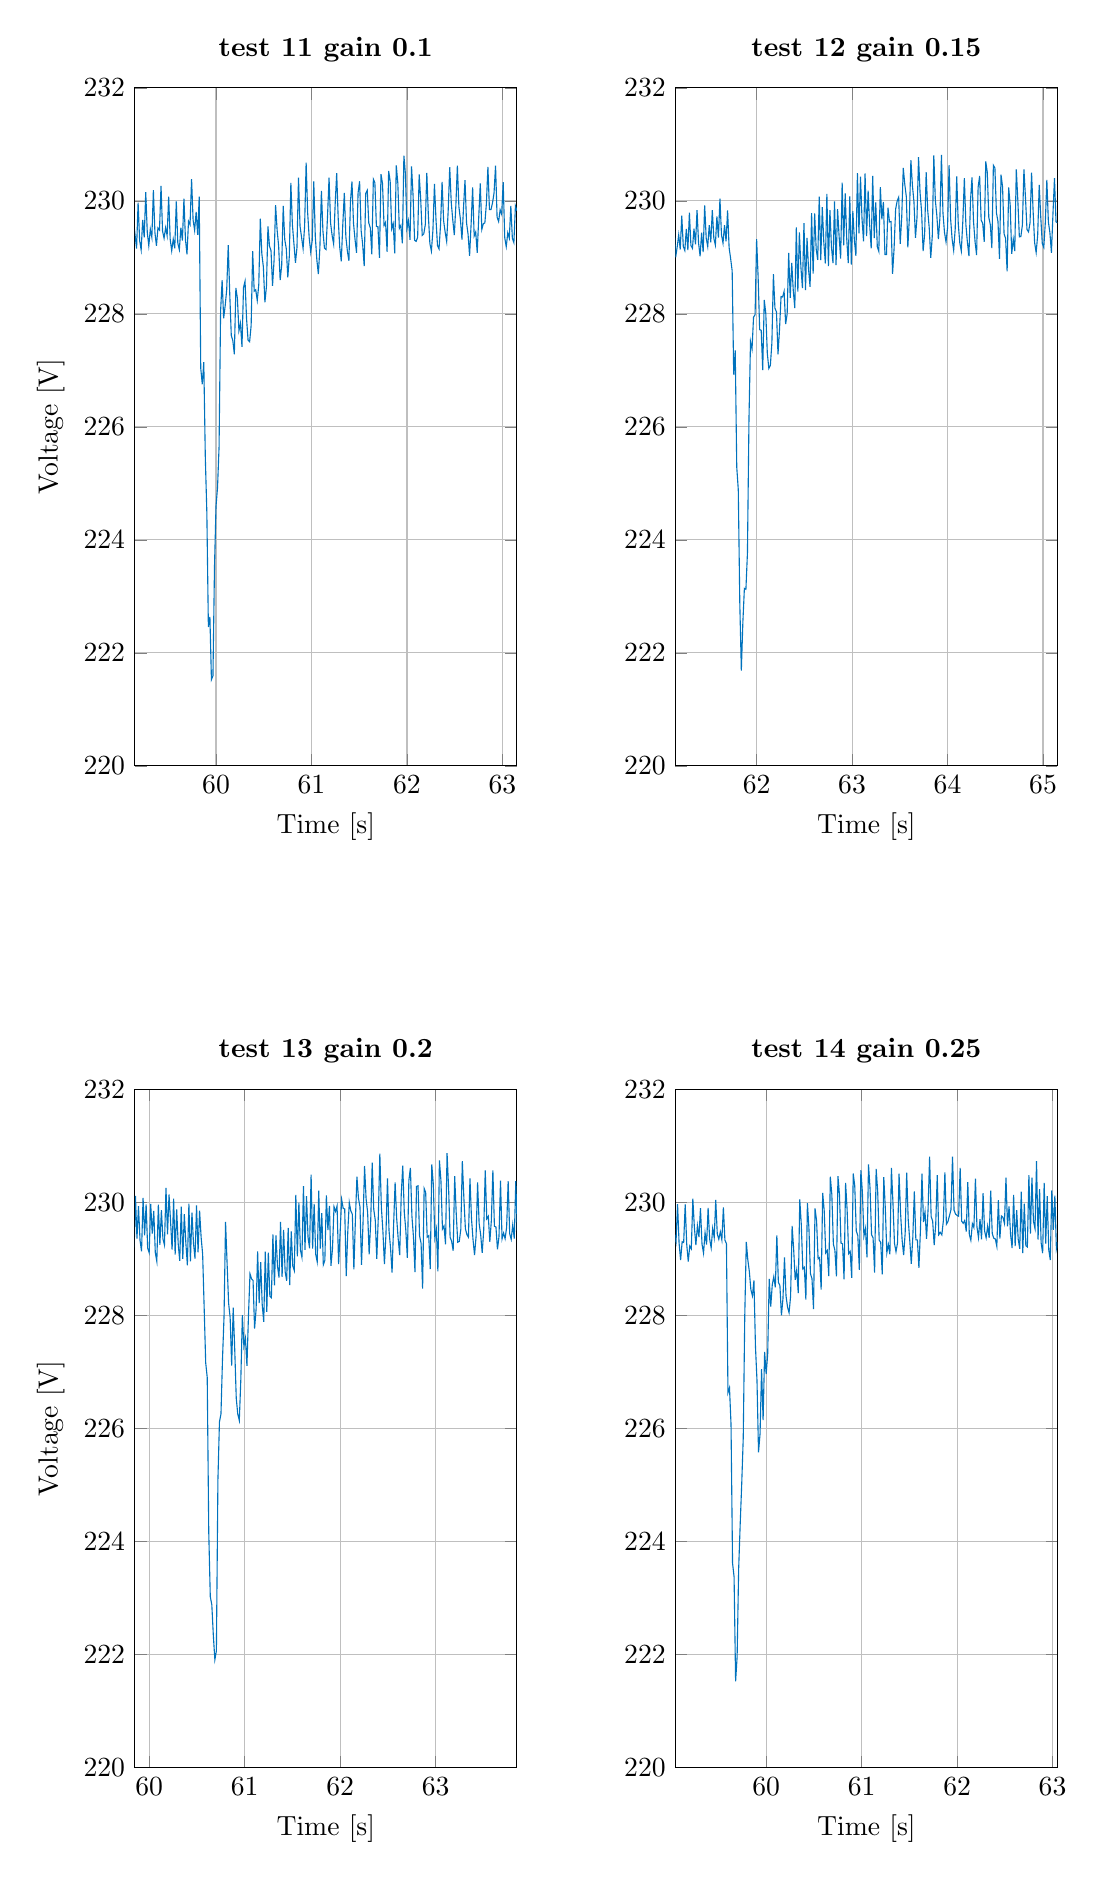
\begin{tikzpicture}

\begin{axis}[%
width=0.4\textwidth,
height=3.39in,
at={(1.297in,5.802in)},
scale only axis,
xmin=59.15,
xmax=63.15,
xlabel={Time [s]},
xmajorgrids,
ymin=220,
ymax=232,
ylabel={Voltage [V]},
ymajorgrids,
axis background/.style={fill=white},
title style={font=\bfseries},
title={test 11 gain 0.1}
]
\addplot [color=mycolor1,solid,forget plot]
  table[row sep=crcr]{%
59.136	229.124402740843\\
59.152	229.400553229391\\
59.168	229.155238286514\\
59.184	229.970098398173\\
59.2	229.297130772027\\
59.216	229.131994773019\\
59.232	229.664740753454\\
59.248	229.352657945567\\
59.264	230.152822917605\\
59.28	229.443578953077\\
59.296	229.205061604623\\
59.312	229.497782165801\\
59.328	229.35359809638\\
59.344	230.188152956178\\
59.36	229.442545523476\\
59.376	229.204441523074\\
59.392	229.522750950399\\
59.408	229.485187940829\\
59.424	230.266663296365\\
59.44	229.466711928108\\
59.456	229.338459231351\\
59.472	229.523968947339\\
59.488	229.38542763652\\
59.504	230.075101485517\\
59.52	229.32207240681\\
59.536	229.11646425537\\
59.552	229.32182453286\\
59.568	229.159219844882\\
59.584	229.989776837008\\
59.6	229.249177985104\\
59.616	229.135578977132\\
59.632	229.526463282292\\
59.648	229.297832144463\\
59.664	230.038493339552\\
59.68	229.314151811537\\
59.696	229.052650563308\\
59.712	229.639177746803\\
59.728	229.579806617385\\
59.744	230.385996022471\\
59.76	229.661446585509\\
59.776	229.47871436731\\
59.792	229.804893752865\\
59.808	229.396881775437\\
59.824	230.07301577965\\
59.84	227.040598232009\\
59.856	226.75517483129\\
59.872	227.144069359468\\
59.888	225.456323218777\\
59.904	224.482430034302\\
59.92	222.45867976645\\
59.936	222.637030413074\\
59.952	221.527303204202\\
59.968	221.594371228426\\
59.984	223.514314034823\\
60	224.595963620475\\
60.016	224.930233560879\\
60.032	225.647590888675\\
60.048	228.047476763245\\
60.064	228.597719676742\\
60.08	227.920657094061\\
60.096	228.14287839712\\
60.112	228.428705044645\\
60.128	229.214747952068\\
60.144	228.349490410531\\
60.16	227.616166576093\\
60.176	227.528795008788\\
60.192	227.285087657107\\
60.208	228.457606915899\\
60.224	228.275079006228\\
60.24	227.700260758675\\
60.256	227.833575207592\\
60.272	227.414843866185\\
60.288	228.46579505321\\
60.304	228.578635213881\\
60.32	227.911650127945\\
60.336	227.531933127807\\
60.352	227.50737223118\\
60.368	227.794784393036\\
60.384	229.110054234143\\
60.4	228.400432722567\\
60.416	228.426360919424\\
60.432	228.238264670226\\
60.448	228.517100089335\\
60.464	229.684406672852\\
60.48	229.061980508356\\
60.496	228.830719227315\\
60.512	228.205368224979\\
60.528	228.476719678932\\
60.544	229.546977479469\\
60.56	229.200154055962\\
60.576	229.120817399766\\
60.592	228.497169770246\\
60.608	228.943562150114\\
60.624	229.92483144223\\
60.64	229.484847211341\\
60.656	229.201182612235\\
60.672	228.596496905877\\
60.688	228.861159149381\\
60.704	229.90972651901\\
60.72	229.316049498203\\
60.736	229.15372802606\\
60.752	228.644466054311\\
60.768	229.025241572977\\
60.784	230.319934413096\\
60.8	229.579774158608\\
60.816	229.244982899859\\
60.832	228.905019444159\\
60.848	229.173762326899\\
60.864	230.411760881102\\
60.88	229.551360886456\\
60.896	229.356455450031\\
60.912	229.157052243216\\
60.928	229.549049592381\\
60.944	230.676497152326\\
60.96	229.786152994682\\
60.976	229.349916516857\\
60.992	229.093827104983\\
61.008	229.301932212611\\
61.024	230.343944100575\\
61.04	229.368544721848\\
61.056	228.959528149602\\
61.072	228.702789121528\\
61.088	229.166915022072\\
61.104	230.177650639555\\
61.12	229.463812435017\\
61.136	229.162976816454\\
61.152	229.139916749887\\
61.168	229.726673618174\\
61.184	230.410225800482\\
61.2	229.607786789832\\
61.216	229.389296154043\\
61.232	229.236460400933\\
61.248	229.93844786627\\
61.264	230.491485249688\\
61.28	229.683129877896\\
61.296	229.179247329946\\
61.312	228.930838867129\\
61.328	229.580753262685\\
61.344	230.1421908875\\
61.36	229.364925731744\\
61.376	229.111846811538\\
61.392	228.938106436381\\
61.408	229.980693104946\\
61.424	230.342212149865\\
61.44	229.606332166398\\
61.456	229.318009685965\\
61.472	229.082107166484\\
61.488	230.143531848732\\
61.504	230.346425116771\\
61.52	229.476197168359\\
61.536	229.229182116261\\
61.552	228.845343725706\\
61.568	230.130553822231\\
61.584	230.187448894506\\
61.6	229.609735501514\\
61.616	229.523187270934\\
61.632	229.054087265349\\
61.648	230.383984371015\\
61.664	230.32255166432\\
61.68	229.547996393007\\
61.696	229.54401312169\\
61.712	228.993334895688\\
61.728	230.473572956445\\
61.744	230.304127493458\\
61.76	229.563773861741\\
61.776	229.620288709474\\
61.792	229.098858429182\\
61.808	230.53056402029\\
61.824	230.352711035006\\
61.84	229.50833946475\\
61.856	229.597447425786\\
61.872	229.072188477173\\
61.888	230.627595697224\\
61.904	230.323051478724\\
61.92	229.511368049858\\
61.936	229.566804704967\\
61.952	229.246660932076\\
61.968	230.801295676614\\
61.984	230.472313143722\\
62	229.510401493433\\
62.016	229.646370263248\\
62.032	229.311092989246\\
62.048	230.610051031701\\
62.064	230.09411285713\\
62.08	229.303001139637\\
62.096	229.283225002196\\
62.112	229.355838388359\\
62.128	230.468346060963\\
62.144	230.02592536616\\
62.16	229.390645683257\\
62.176	229.415360730395\\
62.192	229.577245417684\\
62.208	230.497026283474\\
62.224	229.746235198911\\
62.24	229.245586562992\\
62.256	229.110355500594\\
62.272	229.478738291576\\
62.288	230.299152121744\\
62.304	229.673528307112\\
62.32	229.206614751813\\
62.336	229.148032764606\\
62.352	229.580358080863\\
62.368	230.334516315021\\
62.384	229.646467880608\\
62.4	229.448628730233\\
62.416	229.28161529618\\
62.432	229.832477414234\\
62.448	230.594684505901\\
62.464	229.971487102299\\
62.48	229.66023745052\\
62.496	229.394768892671\\
62.512	229.910926952962\\
62.528	230.625079738033\\
62.544	229.896363534416\\
62.56	229.67303462034\\
62.576	229.314020674396\\
62.592	229.864072684972\\
62.608	230.368678333058\\
62.624	229.613237855509\\
62.64	229.410806829891\\
62.656	229.026683897563\\
62.672	229.591115163077\\
62.688	230.237506208042\\
62.704	229.378876575701\\
62.72	229.44861997649\\
62.736	229.082248589626\\
62.752	229.714427096945\\
62.768	230.30815924368\\
62.784	229.493836159077\\
62.8	229.595993205735\\
62.816	229.609821734027\\
62.832	229.950645764553\\
62.848	230.603314087505\\
62.864	229.847145398898\\
62.88	229.844798091964\\
62.896	229.962639485894\\
62.912	230.137548397655\\
62.928	230.623418209487\\
62.944	229.712328146085\\
62.96	229.634027075321\\
62.976	229.842940774846\\
62.992	229.763050668177\\
63.008	230.330029635796\\
63.024	229.349197089711\\
63.04	229.189564834601\\
63.056	229.435631759813\\
63.072	229.341434481374\\
63.088	229.908921311128\\
63.104	229.336620001868\\
63.12	229.261222734067\\
63.136	229.909115823305\\
63.152	229.826566015293\\
};
\end{axis}

\begin{axis}[%
width=0.4\textwidth,
height=3.39in,
at={(4in,5.802in)},
scale only axis,
xmin=61.15,
xmax=65.15,
xlabel={Time [s]},
xmajorgrids,
ymin=220,
ymax=232,
ymajorgrids,
axis background/.style={fill=white},
title style={font=\bfseries},
title={test 12  gain 0.15}
]
\addplot [color=mycolor1,solid,forget plot]
  table[row sep=crcr]{%
61.136	229.74726705613\\
61.152	229.000982067589\\
61.168	229.183269272052\\
61.184	229.397682789686\\
61.2	229.140111203733\\
61.216	229.738953021296\\
61.232	229.195963473182\\
61.248	229.121625214877\\
61.264	229.505614478007\\
61.28	229.128215149331\\
61.296	229.789541123962\\
61.312	229.211420910749\\
61.328	229.159897110136\\
61.344	229.506146508671\\
61.36	229.229266498771\\
61.376	229.837200779133\\
61.392	229.256082817321\\
61.408	229.020015769979\\
61.424	229.436377385318\\
61.44	229.093746662305\\
61.456	229.919159907578\\
61.472	229.339896124787\\
61.488	229.192902047314\\
61.504	229.571385352465\\
61.52	229.267097275533\\
61.536	229.835524107606\\
61.552	229.335271511261\\
61.568	229.218369129374\\
61.584	229.724106102151\\
61.6	229.348684421042\\
61.616	230.040433455539\\
61.632	229.400175392725\\
61.648	229.25167889405\\
61.664	229.571494542312\\
61.68	229.283192083256\\
61.696	229.830412816039\\
61.712	229.171384840921\\
61.728	228.977405030387\\
61.744	228.76057594009\\
61.76	226.925180350901\\
61.776	227.35321086096\\
61.792	225.287352749512\\
61.808	224.889784326452\\
61.824	222.869758637971\\
61.84	221.687461498395\\
61.856	222.541545982731\\
61.872	223.141504384402\\
61.888	223.12624132173\\
61.904	223.769279188799\\
61.92	226.13556551445\\
61.936	227.51201581385\\
61.952	227.375406786766\\
61.968	227.942644406796\\
61.984	227.985302159105\\
62	229.323593159412\\
62.016	228.646086823245\\
62.032	227.720763966006\\
62.048	227.710175361873\\
62.064	227.00526702034\\
62.08	228.245114452137\\
62.096	228.013150472782\\
62.112	227.305193243246\\
62.128	227.032804667813\\
62.144	227.087144820754\\
62.16	227.486167414668\\
62.176	228.701679941438\\
62.192	228.099762504725\\
62.208	228.035507384949\\
62.224	227.283000364621\\
62.24	227.726544273897\\
62.256	228.306663658195\\
62.272	228.29877987051\\
62.288	228.397931522088\\
62.304	227.8186955258\\
62.32	227.999823482332\\
62.336	229.077227692131\\
62.352	228.284798879123\\
62.368	228.90267135373\\
62.384	228.413091596127\\
62.4	228.103953439738\\
62.416	229.530988903724\\
62.432	228.394285776954\\
62.448	229.441339199072\\
62.464	228.825709407708\\
62.48	228.455772076279\\
62.496	229.60597886719\\
62.512	228.421755461542\\
62.528	229.345003693584\\
62.544	228.792837936488\\
62.56	228.476690185444\\
62.576	229.784184671767\\
62.592	228.711447286919\\
62.608	229.776618975097\\
62.624	229.148735915351\\
62.64	228.954720722739\\
62.656	230.07342172063\\
62.672	228.95004726834\\
62.688	229.888205170649\\
62.704	229.261767230289\\
62.72	228.891937591592\\
62.736	230.123172172595\\
62.752	228.84487737937\\
62.768	229.836454250483\\
62.784	229.182775375823\\
62.8	228.897494964113\\
62.816	229.991616716913\\
62.832	228.862603172463\\
62.848	229.854505874793\\
62.864	229.37598409399\\
62.88	228.978607591755\\
62.896	230.322847412468\\
62.912	229.213192375876\\
62.928	230.13229874149\\
62.944	229.322536353419\\
62.96	228.896693708936\\
62.976	230.080943849766\\
62.992	228.873236292242\\
63.008	229.817053861109\\
63.024	229.30307080817\\
63.04	229.026646667878\\
63.056	230.489229707445\\
63.072	229.425368842705\\
63.088	230.429292021511\\
63.104	229.682968653315\\
63.12	229.282844721215\\
63.136	230.488371861841\\
63.152	229.37580002218\\
63.168	230.181516941236\\
63.184	229.582195137431\\
63.2	229.160324141043\\
63.216	230.443346456405\\
63.232	229.341922989358\\
63.248	229.972061462205\\
63.264	229.188825906051\\
63.28	229.105851674543\\
63.296	230.244184585671\\
63.312	229.674447947605\\
63.328	229.979571173318\\
63.344	229.051646367888\\
63.36	229.050598228717\\
63.376	229.877722963254\\
63.392	229.626764688568\\
63.408	229.634779711737\\
63.424	228.708350904728\\
63.44	229.160440848642\\
63.456	229.851632846235\\
63.472	229.996357295837\\
63.488	230.063696240148\\
63.504	229.239005314531\\
63.52	229.712006431614\\
63.536	230.582456739274\\
63.552	230.293926718295\\
63.568	230.075944810876\\
63.584	229.1767392189\\
63.6	229.702105489495\\
63.616	230.722727190428\\
63.632	230.272962388315\\
63.648	229.983448849417\\
63.664	229.347073384636\\
63.68	229.706671622902\\
63.696	230.775627353153\\
63.712	230.144383778383\\
63.728	229.814605276738\\
63.744	229.112927237405\\
63.76	229.413524893494\\
63.776	230.507099450074\\
63.792	229.835572675483\\
63.808	229.519933689168\\
63.824	228.989943672156\\
63.84	229.375366005573\\
63.856	230.806180094097\\
63.872	230.011863554003\\
63.888	229.737217368715\\
63.904	229.322234171431\\
63.92	229.699840028688\\
63.936	230.812989947006\\
63.952	229.782997344979\\
63.968	229.43952541474\\
63.984	229.272217067298\\
64	229.523183449264\\
64.016	230.633985933491\\
64.032	229.681603508597\\
64.048	229.320961648897\\
64.064	229.124479435671\\
64.08	229.501516495554\\
64.096	230.433082440938\\
64.112	229.596514494646\\
64.128	229.259352629801\\
64.144	229.11208451754\\
64.16	229.639818514421\\
64.176	230.402031983288\\
64.192	229.57885574108\\
64.208	229.26578518703\\
64.224	229.024485078031\\
64.24	229.998146530983\\
64.256	230.415898480736\\
64.272	229.635814720653\\
64.288	229.277756896317\\
64.304	229.0420926361\\
64.32	230.240787390199\\
64.336	230.440160851961\\
64.352	229.657307910439\\
64.368	229.601890894525\\
64.384	229.276964174602\\
64.4	230.696614719419\\
64.416	230.506916456319\\
64.432	229.709988006854\\
64.448	229.57808505588\\
64.464	229.163180265574\\
64.48	230.629558425434\\
64.496	230.582269200852\\
64.512	229.786206487659\\
64.528	229.637285649621\\
64.544	228.972378365407\\
64.56	230.463192172045\\
64.576	230.251679573132\\
64.592	229.415604055261\\
64.608	229.334837526187\\
64.624	228.752140776427\\
64.64	230.23805287505\\
64.656	229.925373887873\\
64.672	229.061543481521\\
64.688	229.322708453218\\
64.704	229.112500250302\\
64.72	230.556129386367\\
64.736	230.01504866719\\
64.752	229.362662469042\\
64.768	229.368949190952\\
64.784	229.57581475422\\
64.8	230.559082129234\\
64.816	230.062303106786\\
64.832	229.493569203895\\
64.848	229.451330850515\\
64.864	229.615421037327\\
64.88	230.497547090498\\
64.896	229.822835051935\\
64.912	229.259161780432\\
64.928	229.086708149813\\
64.944	229.392508201011\\
64.96	230.281882384516\\
64.976	229.719089512381\\
64.992	229.247170964021\\
65.008	229.176508197108\\
65.024	229.616473305266\\
65.04	230.371065726741\\
65.056	229.627543051907\\
65.072	229.439280974484\\
65.088	229.081272000532\\
65.104	229.769019917343\\
65.12	230.402047428448\\
65.136	229.629213992999\\
65.152	229.609566736592\\
};
\end{axis}

\begin{axis}[%
width=0.4\textwidth,
height=3.39in,
at={(1.297in,0.793in)},
scale only axis,
xmin=59.85,
xmax=63.85,
xlabel={Time [s]},
xmajorgrids,
ymin=220,
ymax=232,
ylabel={Voltage [V]},
ymajorgrids,
axis background/.style={fill=white},
title style={font=\bfseries},
title={test 13  gain 0.2}
]
\addplot [color=mycolor1,solid,forget plot]
  table[row sep=crcr]{%
59.84	228.9950921353\\
59.856	230.120397872899\\
59.872	229.364175307407\\
59.888	229.940466386841\\
59.904	229.335916985954\\
59.92	229.138197347007\\
59.936	230.086074820849\\
59.952	229.422248005847\\
59.968	229.971329238591\\
59.984	229.197828462908\\
60	229.114608759003\\
60.016	229.977235452781\\
60.032	229.451185698698\\
60.048	229.853722419343\\
60.064	229.116065509844\\
60.08	228.961927736596\\
60.096	229.966862494195\\
60.112	229.253516157476\\
60.128	229.869760448522\\
60.144	229.361669530576\\
60.16	229.250941747047\\
60.176	230.259865360821\\
60.192	229.438909341316\\
60.208	230.144122408849\\
60.224	229.667047552846\\
60.24	229.167283926006\\
60.256	230.06987511584\\
60.272	229.08292488949\\
60.288	229.88289726309\\
60.304	229.27147812105\\
60.32	228.970309482689\\
60.336	229.928516710305\\
60.352	229.003390962414\\
60.368	229.795541463709\\
60.384	229.288545829128\\
60.4	228.892103305257\\
60.416	229.980831752877\\
60.432	228.962085843402\\
60.448	229.825152301887\\
60.464	229.285070779018\\
60.48	229.010388958736\\
60.496	229.95070019234\\
60.512	229.122459426906\\
60.528	229.859408414761\\
60.544	229.388299039069\\
60.56	229.08713585869\\
60.576	228.133431475908\\
60.592	227.166274277302\\
60.608	226.906489558287\\
60.624	224.167688050573\\
60.64	223.026567063451\\
60.656	222.88473985603\\
60.672	222.339870508143\\
60.688	221.911526610546\\
60.704	222.067347188493\\
60.72	225.0957546017\\
60.736	226.120411769502\\
60.752	226.260870613631\\
60.768	227.235216665951\\
60.784	227.982475989121\\
60.8	229.660336045849\\
60.816	228.928520867831\\
60.832	228.220872552348\\
60.848	227.967386760566\\
60.864	227.118238789743\\
60.88	228.142560453528\\
60.896	227.409514752494\\
60.912	226.537974275672\\
60.928	226.255886055767\\
60.944	226.145214278368\\
60.96	226.873741974476\\
60.976	228.010010760298\\
60.992	227.45873498012\\
61.008	227.600001662357\\
61.024	227.111679072256\\
61.04	228.00300833456\\
61.056	228.740942752332\\
61.072	228.652941133567\\
61.088	228.622386552346\\
61.104	227.769352154973\\
61.12	228.118289560159\\
61.136	229.135837852742\\
61.152	228.220797662445\\
61.168	228.945920465877\\
61.184	228.192616134971\\
61.2	227.889301905302\\
61.216	229.132251784088\\
61.232	228.065914594577\\
61.248	229.114448490735\\
61.264	228.342804931295\\
61.28	228.31687126618\\
61.296	229.440057330725\\
61.312	228.535093225844\\
61.328	229.419389474201\\
61.344	228.876025662248\\
61.36	228.676059002518\\
61.376	229.661593940954\\
61.392	228.685752196931\\
61.408	229.51886015032\\
61.424	228.778848412419\\
61.44	228.61637209274\\
61.456	229.553530239565\\
61.472	228.542570531543\\
61.488	229.491574246605\\
61.504	228.879863406335\\
61.52	228.798477433283\\
61.536	230.138782862883\\
61.552	229.051408949803\\
61.568	230.000555605904\\
61.584	229.161845603482\\
61.6	229.032896885949\\
61.616	230.292553798254\\
61.632	229.16619101939\\
61.648	230.117644678647\\
61.664	229.385809437571\\
61.68	229.191295828954\\
61.696	230.49406071159\\
61.712	229.188999098157\\
61.728	229.978928786219\\
61.744	229.08828547193\\
61.76	228.951688858898\\
61.776	230.214099814731\\
61.792	229.188420049207\\
61.808	229.814824067583\\
61.824	228.900285829202\\
61.84	228.97852292832\\
61.856	230.126746920098\\
61.872	229.515543075165\\
61.888	229.944259317699\\
61.904	228.881980255664\\
61.92	229.184873207173\\
61.936	229.927467891765\\
61.952	229.845202431705\\
61.968	229.940989436073\\
61.984	228.912551807909\\
62	229.472375660284\\
62.016	230.056717644201\\
62.032	229.899592970853\\
62.048	229.889159473006\\
62.064	228.699090124781\\
62.08	229.478690176916\\
62.096	230.003741766515\\
62.112	229.854539942721\\
62.128	229.794693484999\\
62.144	228.820089255918\\
62.16	229.6956536206\\
62.176	230.460746902038\\
62.192	230.079469480901\\
62.208	229.924136344668\\
62.224	228.899330915269\\
62.24	229.649561262358\\
62.256	230.648686886928\\
62.272	230.068739134806\\
62.288	229.830873662947\\
62.304	229.08549602293\\
62.32	229.652150757358\\
62.336	230.707685367705\\
62.352	229.884474782546\\
62.368	229.691255964218\\
62.384	229.005014360446\\
62.4	229.754112090761\\
62.416	230.867082975747\\
62.432	229.920224002338\\
62.448	229.496345551251\\
62.464	228.913957773305\\
62.48	229.438671044424\\
62.496	230.428655702315\\
62.512	229.510990225522\\
62.528	229.194822612048\\
62.544	228.762281255526\\
62.56	229.593616785579\\
62.576	230.360679482993\\
62.592	229.729246414302\\
62.608	229.364978118263\\
62.624	229.071193454262\\
62.64	230.137086334752\\
62.656	230.656417865943\\
62.672	229.832409930239\\
62.688	229.514313122111\\
62.704	229.022535794119\\
62.72	230.393471026381\\
62.736	230.614441699769\\
62.752	229.762590455947\\
62.768	229.397238373679\\
62.784	228.772941276209\\
62.8	230.286849728362\\
62.816	230.298276436356\\
62.832	229.413768180294\\
62.848	229.280852471955\\
62.864	228.478183993307\\
62.88	230.251931210756\\
62.896	230.181221513644\\
62.912	229.390005823209\\
62.928	229.417010506133\\
62.944	228.826223883764\\
62.96	230.675179632397\\
62.976	230.328424329995\\
62.992	229.377051966197\\
63.008	229.528841628564\\
63.024	228.784900892082\\
63.04	230.749501854115\\
63.056	230.387597560787\\
63.072	229.53303184908\\
63.088	229.58740784537\\
63.104	229.264315350291\\
63.12	230.878222240564\\
63.136	230.268223287169\\
63.152	229.386054079739\\
63.168	229.318109826811\\
63.184	229.149724007088\\
63.2	230.468527504517\\
63.216	229.811210280639\\
63.232	229.300535751004\\
63.248	229.314360492412\\
63.264	229.526810285484\\
63.28	230.736340483237\\
63.296	230.090359503849\\
63.312	229.540184099988\\
63.328	229.434646105056\\
63.344	229.387783214853\\
63.36	230.429155004069\\
63.376	229.718790403574\\
63.392	229.346459510051\\
63.408	229.071444009859\\
63.424	229.404031763269\\
63.44	230.358047940028\\
63.456	229.632183225189\\
63.472	229.436308685094\\
63.488	229.111379395463\\
63.504	229.511215996799\\
63.52	230.571123637588\\
63.536	229.714025062526\\
63.552	229.759290665192\\
63.568	229.306309318674\\
63.584	229.684788300841\\
63.6	230.573343953275\\
63.616	229.582024204109\\
63.632	229.570454275478\\
63.648	229.173398654558\\
63.664	229.400235640331\\
63.68	230.391863125208\\
63.696	229.357966938123\\
63.712	229.462767805902\\
63.728	229.363297449485\\
63.744	229.563662200528\\
63.76	230.382462381394\\
63.776	229.451258124979\\
63.792	229.350909090345\\
63.808	229.608671666551\\
63.824	229.362790764597\\
63.84	230.379966919101\\
63.856	229.50060463372\\
};
\end{axis}

\begin{axis}[%
width=0.4\textwidth,
height=3.39in,
at={(4in,0.793in)},
scale only axis,
xmin=59.05,
xmax=63.05,
xlabel={Time [s]},
xmajorgrids,
ymin=220,
ymax=232,
ymajorgrids,
axis background/.style={fill=white},
title style={font=\bfseries},
title={test 14  gain 0.25}
]
\addplot [color=mycolor1,solid,forget plot]
  table[row sep=crcr]{%
59.04	229.457525474607\\
59.056	229.30889337919\\
59.072	229.974571275079\\
59.088	229.283196501694\\
59.104	228.98270469108\\
59.12	229.308040597165\\
59.136	229.295968986188\\
59.152	229.969312640749\\
59.168	229.262452851752\\
59.184	228.957093404943\\
59.2	229.233674521015\\
59.216	229.184459964082\\
59.232	230.072464760778\\
59.248	229.56409407227\\
59.264	229.249987289427\\
59.28	229.592603001323\\
59.296	229.392314818733\\
59.312	229.902954604965\\
59.328	229.267751049547\\
59.344	229.107733216095\\
59.36	229.469448778594\\
59.376	229.260177479303\\
59.392	229.905673246418\\
59.408	229.359704561544\\
59.424	229.199750333517\\
59.44	229.545482957017\\
59.456	229.382227583124\\
59.472	230.04960339884\\
59.488	229.448855952228\\
59.504	229.352436670139\\
59.52	229.483723249569\\
59.536	229.341148359481\\
59.552	229.917912787614\\
59.568	229.336272085804\\
59.584	229.27621671704\\
59.6	226.636693989251\\
59.616	226.724881314842\\
59.632	226.07736726437\\
59.648	223.62125131807\\
59.664	223.376574128624\\
59.68	221.526290055142\\
59.696	221.968236730388\\
59.712	223.518884845864\\
59.728	224.306232570453\\
59.744	225.018440366915\\
59.76	225.836303956056\\
59.776	228.000693035864\\
59.792	229.306958838043\\
59.808	228.988020346748\\
59.824	228.781569991296\\
59.84	228.459228661639\\
59.856	228.351240826332\\
59.872	228.623089460423\\
59.888	227.453870969246\\
59.904	226.851479012848\\
59.92	225.582375601646\\
59.936	225.905769442858\\
59.952	227.051578562128\\
59.968	226.149575738824\\
59.984	227.357654094205\\
60	226.968069635608\\
60.016	227.317008242253\\
60.032	228.650515089103\\
60.048	228.162221521321\\
60.064	228.545197439636\\
60.08	228.691195034684\\
60.096	228.500705197101\\
60.112	229.423017017877\\
60.128	228.590483185252\\
60.144	228.532928296692\\
60.16	228.005342364951\\
60.176	228.301283489893\\
60.192	229.032142115478\\
60.208	228.350515776685\\
60.224	228.151764686237\\
60.24	228.051343127292\\
60.256	228.345812705775\\
60.272	229.587021818613\\
60.288	229.179449046505\\
60.304	228.633571945914\\
60.32	228.812751143924\\
60.336	228.40135283972\\
60.352	230.059372354262\\
60.368	229.614921327777\\
60.384	228.825533088179\\
60.4	228.853824243723\\
60.416	228.28527864483\\
60.432	229.993206474696\\
60.448	229.545737459978\\
60.464	228.740255737634\\
60.48	228.657166938148\\
60.496	228.116417388677\\
60.512	229.896834519355\\
60.528	229.684244016587\\
60.544	229.00518123721\\
60.56	229.028514474405\\
60.576	228.463045242747\\
60.592	230.174591815313\\
60.608	229.856833318342\\
60.624	229.112508937397\\
60.64	229.155854718046\\
60.656	228.701520808237\\
60.672	230.458355631867\\
60.688	230.142125817663\\
60.704	229.267093363445\\
60.72	229.158016369761\\
60.736	228.697380730908\\
60.752	230.469062023768\\
60.768	230.139317240399\\
60.784	229.28425656757\\
60.8	229.272007988465\\
60.816	228.643064733287\\
60.832	230.349335386822\\
60.848	229.877657212184\\
60.864	229.098434986863\\
60.88	229.137970608882\\
60.896	228.669083344616\\
60.912	230.515410417222\\
60.928	230.295476321498\\
60.944	229.497469413317\\
60.96	229.4164686912\\
60.976	228.810603330434\\
60.992	230.577033328529\\
61.008	230.18201694136\\
61.024	229.408258533288\\
61.04	229.541804059499\\
61.056	229.03377812102\\
61.072	230.677646984274\\
61.088	230.254453487881\\
61.104	229.433730074329\\
61.12	229.377144597775\\
61.136	228.760743859577\\
61.152	230.596038839152\\
61.168	230.204968437363\\
61.184	229.336824268117\\
61.2	229.295985132405\\
61.216	228.732065155441\\
61.232	230.451515238943\\
61.248	229.902349147795\\
61.264	229.111718119707\\
61.28	229.259079516189\\
61.296	229.085735911812\\
61.312	230.614805257773\\
61.328	230.002343242915\\
61.344	229.279935545221\\
61.36	229.132291707341\\
61.376	229.287703949897\\
61.392	230.512095624599\\
61.408	229.81453513873\\
61.424	229.342575949347\\
61.44	229.071273898094\\
61.456	229.458482805804\\
61.472	230.530159591336\\
61.488	229.695917538822\\
61.504	229.334603808811\\
61.52	228.918964923136\\
61.536	229.383597416453\\
61.552	230.199228216126\\
61.568	229.343631375357\\
61.584	229.339140079721\\
61.6	228.845726029107\\
61.616	229.513970351781\\
61.632	230.514609867192\\
61.648	229.655578752648\\
61.664	229.838963744821\\
61.68	229.358696415594\\
61.696	229.885058141171\\
61.712	230.814584080762\\
61.728	229.754919188966\\
61.744	229.674433864404\\
61.76	229.247677113631\\
61.776	229.614098649209\\
61.792	230.488109759179\\
61.808	229.432100219789\\
61.824	229.474837844503\\
61.84	229.430313594594\\
61.856	229.676461927025\\
61.872	230.536365023162\\
61.888	229.619263570323\\
61.904	229.664220475905\\
61.92	229.770091380257\\
61.936	229.875362710166\\
61.952	230.815411278521\\
61.968	229.867602299913\\
61.984	229.797554681213\\
62	229.774005379655\\
62.016	229.75921806749\\
62.032	230.615073885218\\
62.048	229.672479884304\\
62.064	229.634870339703\\
62.08	229.685357032491\\
62.096	229.490133169016\\
62.112	230.363706738305\\
62.128	229.436954328709\\
62.144	229.332839464909\\
62.16	229.627063839084\\
62.176	229.559515191932\\
62.192	230.425973143473\\
62.208	229.571374516921\\
62.224	229.382155616052\\
62.24	229.708904902252\\
62.256	229.349687023096\\
62.272	230.167759424693\\
62.288	229.499209634614\\
62.304	229.378469898361\\
62.32	229.585322874495\\
62.336	229.379846330817\\
62.352	230.211930828004\\
62.368	229.455599267454\\
62.384	229.371379728576\\
62.4	229.35807944078\\
62.416	229.228034766481\\
62.432	230.043523833259\\
62.448	229.365564537966\\
62.464	229.764482176529\\
62.48	229.743086601991\\
62.496	229.632965492979\\
62.512	230.442209774023\\
62.528	229.580065866363\\
62.544	229.93365614267\\
62.56	229.437780684175\\
62.576	229.197915443623\\
62.592	230.136980215914\\
62.608	229.230380716672\\
62.624	229.867140146552\\
62.64	229.352867111314\\
62.656	229.184477730607\\
62.672	230.193040285196\\
62.688	229.108697987797\\
62.704	229.981256669271\\
62.72	229.23886379682\\
62.736	229.216283603102\\
62.752	230.489115835894\\
62.768	229.451372685421\\
62.784	230.441121143266\\
62.8	229.671524998686\\
62.816	229.542295145729\\
62.832	230.733485329464\\
62.848	229.347225915315\\
62.864	230.23873321742\\
62.88	229.294203603162\\
62.896	229.10589541706\\
62.912	230.351780928835\\
62.928	229.27582514785\\
62.944	230.115095932577\\
62.96	229.166271480702\\
62.976	228.985819209715\\
62.992	230.2162844923\\
63.008	229.519710832413\\
63.024	230.125365215057\\
63.04	229.179885546826\\
63.056	229.305471112424\\
};
\end{axis}
\end{tikzpicture}%
\caption{Step from 30 to 40 kW load, with various scaling factors.}
\label{fig:test11-14-30to40kwstepvolt}
\end{figure}

\begin{figure}[H]
\centering
% This file was created by matlab2tikz.
%
%The latest updates can be retrieved from
%  http://www.mathworks.com/matlabcentral/fileexchange/22022-matlab2tikz-matlab2tikz
%where you can also make suggestions and rate matlab2tikz.
%
\definecolor{mycolor1}{rgb}{0.00000,0.44700,0.74100}%
%
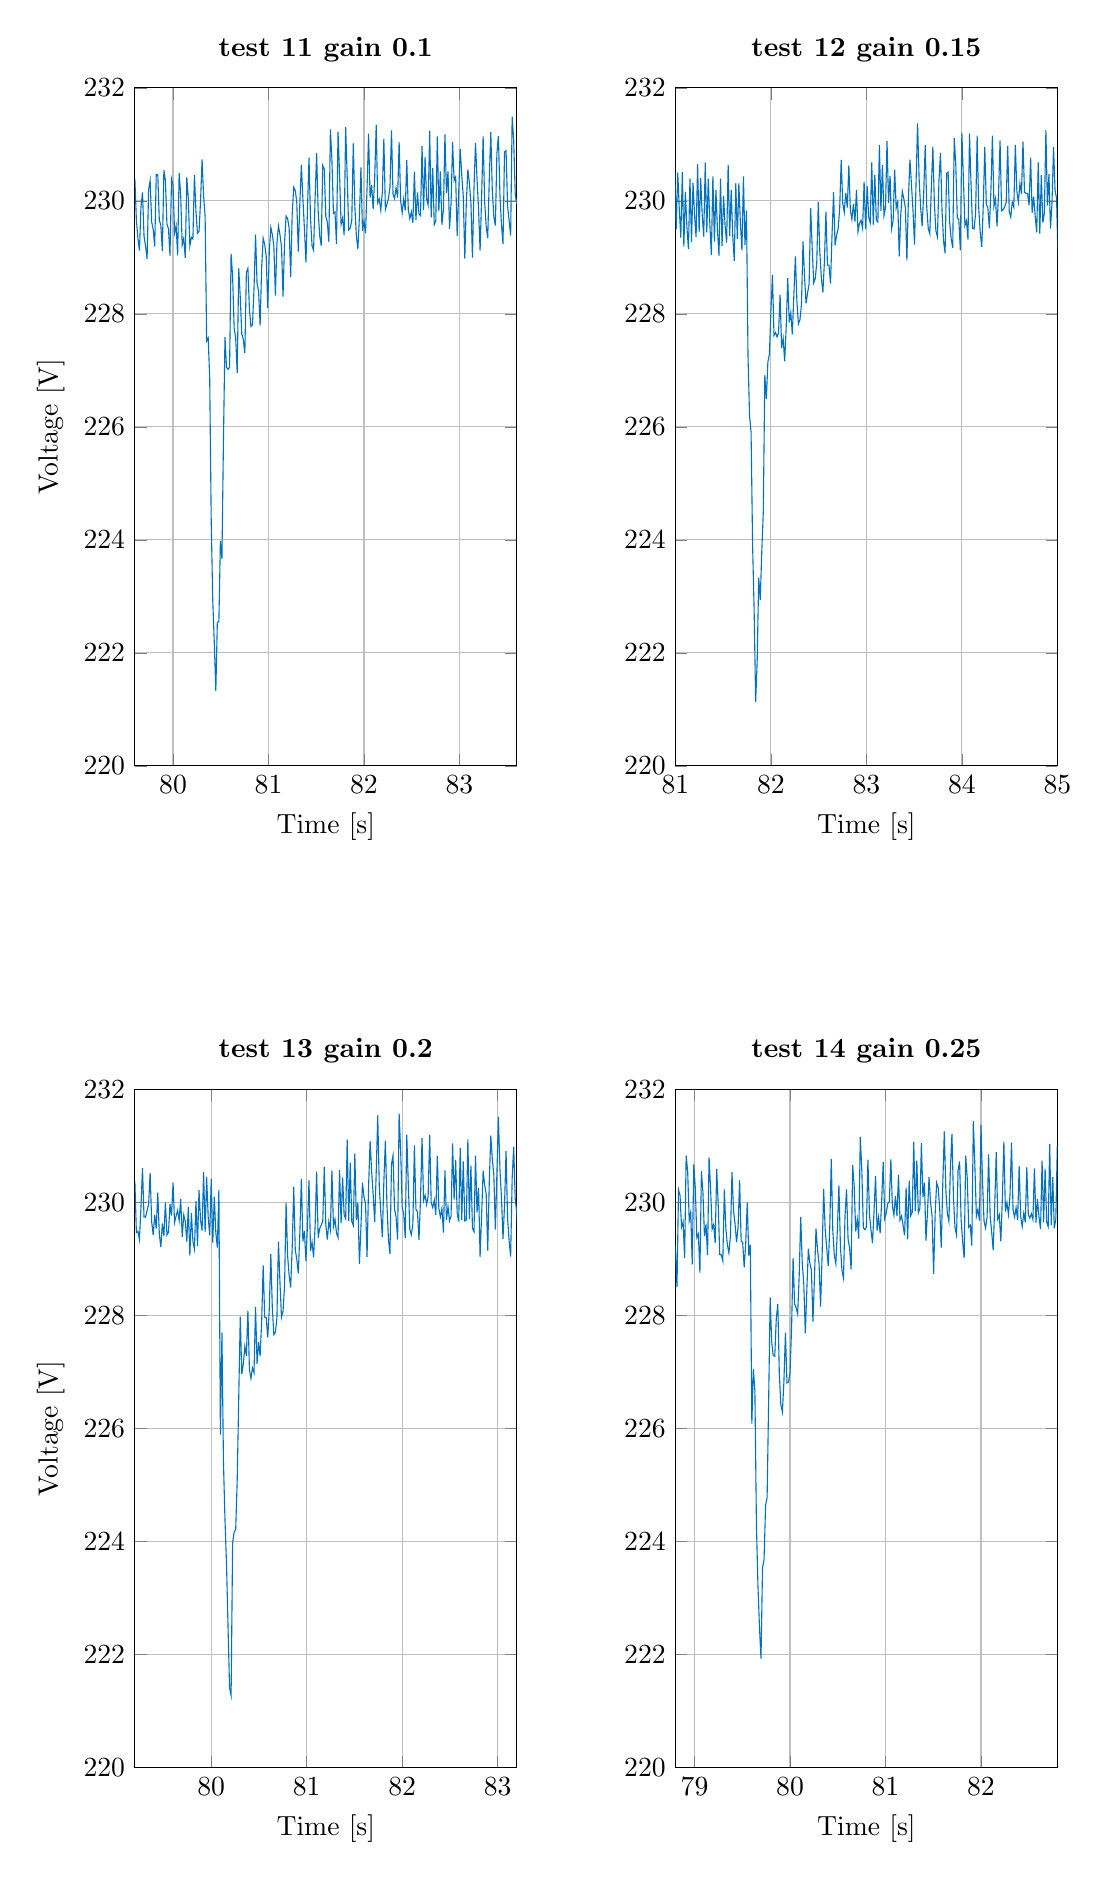
\begin{tikzpicture}

\begin{axis}[%
width=0.4\textwidth,
height=3.39in,
at={(1.297in,5.802in)},
scale only axis,
xmin=79.6,
xmax=83.6,
xlabel={Time [s]},
xmajorgrids,
ymin=220,
ymax=232,
ylabel={Voltage [V]},
ymajorgrids,
axis background/.style={fill=white},
title style={font=\bfseries},
title={test 11 gain 0.1}
]
\addplot [color=mycolor1,solid,forget plot]
  table[row sep=crcr]{%
79.584	230.043595164997\\
79.6	230.392327346044\\
79.616	229.660186785528\\
79.632	229.332855000952\\
79.648	229.121783697983\\
79.664	229.893492133557\\
79.68	230.148134325236\\
79.696	229.378868501535\\
79.712	229.198634876021\\
79.728	228.970542612795\\
79.744	230.201684235725\\
79.76	230.359611286516\\
79.776	229.627733114705\\
79.792	229.492738797686\\
79.808	229.193852566124\\
79.824	230.469088373623\\
79.84	230.456953712428\\
79.856	229.659617359682\\
79.872	229.569946107544\\
79.888	229.111048756185\\
79.904	230.544127144302\\
79.92	230.356808542092\\
79.936	229.5850823534\\
79.952	229.50898758463\\
79.968	229.031325513871\\
79.984	230.38885619579\\
80	230.274995814981\\
80.016	229.430404079701\\
80.032	229.561408405763\\
80.048	229.03785581884\\
80.064	230.494315374119\\
80.08	230.101585786784\\
80.096	229.217474499314\\
80.112	229.336502679851\\
80.128	228.993534292762\\
80.144	230.417175399674\\
80.16	230.04156901302\\
80.176	229.202518195008\\
80.192	229.354840677697\\
80.208	229.326780054588\\
80.224	230.458787654495\\
80.24	229.808597628894\\
80.256	229.427113046164\\
80.272	229.454579556395\\
80.288	229.990076731959\\
80.304	230.733374657206\\
80.32	230.085912858541\\
80.336	229.720827593841\\
80.352	227.520698714948\\
80.368	227.575585532173\\
80.384	226.857059326582\\
80.4	224.300474018765\\
80.416	222.920397330374\\
80.432	222.178171648306\\
80.448	221.327437451402\\
80.464	222.544267339288\\
80.48	222.548962099366\\
80.496	223.980231466105\\
80.512	223.663212819589\\
80.528	225.771384780395\\
80.544	227.589069227632\\
80.56	227.053901678286\\
80.576	227.017374081925\\
80.592	227.054556914651\\
80.608	229.063761827993\\
80.624	228.661012585298\\
80.64	227.748614559905\\
80.656	227.574508265602\\
80.672	226.955816665418\\
80.688	228.802965203106\\
80.704	228.297509918196\\
80.72	227.641663254172\\
80.736	227.548519088007\\
80.752	227.30437992081\\
80.768	228.737247513864\\
80.784	228.805369699677\\
80.8	228.079108648766\\
80.816	227.777257534125\\
80.832	227.806182266279\\
80.848	228.440993473323\\
80.864	229.404252371529\\
80.88	228.538522920094\\
80.896	228.395263624541\\
80.912	227.794191979496\\
80.928	228.825146801581\\
80.944	229.338519333367\\
80.96	229.226406372857\\
80.976	229.016822451359\\
80.992	228.102096537339\\
81.008	229.098492569916\\
81.024	229.530602732923\\
81.04	229.400761548726\\
81.056	229.199723723832\\
81.072	228.32109299858\\
81.088	229.24466617878\\
81.104	229.558406646516\\
81.12	229.399339399684\\
81.136	229.181817539719\\
81.152	228.306958073323\\
81.168	229.257280046909\\
81.184	229.733742804175\\
81.2	229.683661126977\\
81.216	229.520841825595\\
81.232	228.650698906561\\
81.248	229.763934970744\\
81.264	230.240482412386\\
81.28	230.187739236141\\
81.296	229.973569199184\\
81.312	229.101497898597\\
81.328	229.956212919068\\
81.344	230.643114315917\\
81.36	230.037538999355\\
81.376	229.511750155766\\
81.392	228.913356898716\\
81.408	229.840077889636\\
81.424	230.764086061509\\
81.44	229.683699352772\\
81.456	229.204283755213\\
81.472	229.125626757967\\
81.488	230.057966747538\\
81.504	230.843586872558\\
81.52	229.820291014518\\
81.536	229.382623575772\\
81.552	229.208581560346\\
81.568	230.624449718513\\
81.584	230.562368793749\\
81.6	229.726080437389\\
81.616	229.626685527297\\
81.632	229.273872606493\\
81.648	231.264923758306\\
81.664	230.731598494859\\
81.68	229.77741650822\\
81.696	229.804373488513\\
81.712	229.237813632579\\
81.728	231.225571241671\\
81.744	230.474012968512\\
81.76	229.584698174446\\
81.776	229.699901869042\\
81.792	229.39188548342\\
81.808	231.306052304729\\
81.824	230.434609848099\\
81.84	229.4854750137\\
81.856	229.517897494402\\
81.872	229.65727684819\\
81.888	231.019289497187\\
81.904	229.907905783632\\
81.92	229.382951367593\\
81.936	229.147155562394\\
81.952	229.717301109271\\
81.968	230.594060508339\\
81.984	229.468960770787\\
82	229.638989448055\\
82.016	229.429083398919\\
82.032	230.226023638492\\
82.048	231.189743714843\\
82.064	230.058987195031\\
82.08	230.278335895947\\
82.096	229.852762223195\\
82.112	230.413524520515\\
82.128	231.346200392656\\
82.144	229.968880333177\\
82.16	230.032007204561\\
82.176	229.836016809579\\
82.192	230.150901758461\\
82.208	231.099720668919\\
82.224	229.847674726021\\
82.24	229.939900737945\\
82.256	230.041638227831\\
82.272	230.241208935004\\
82.288	231.246556109186\\
82.304	230.123168847351\\
82.32	230.03814340941\\
82.336	230.23002638337\\
82.352	230.060253717255\\
82.368	231.041418985229\\
82.384	229.993679837638\\
82.4	229.788873162557\\
82.416	230.034680668659\\
82.432	229.830666782809\\
82.448	230.722923288544\\
82.464	229.846143343243\\
82.48	229.686285982926\\
82.496	229.805259328636\\
82.512	229.612754640456\\
82.528	230.51848289786\\
82.544	229.662732922722\\
82.56	230.150448363649\\
82.576	229.769792911043\\
82.592	229.738152899553\\
82.608	230.972533786204\\
82.624	229.836702015522\\
82.64	230.774450241162\\
82.656	230.030601298649\\
82.672	229.922313665729\\
82.688	231.244365969709\\
82.704	229.708593400465\\
82.72	230.58418026385\\
82.736	229.579946770092\\
82.752	229.647302970675\\
82.768	231.143130467104\\
82.784	229.818581265534\\
82.8	230.521381111233\\
82.816	229.578083192201\\
82.832	229.846142394007\\
82.848	231.178185183328\\
82.864	230.135604809468\\
82.88	230.520740510058\\
82.896	229.505111839973\\
82.912	229.958431210871\\
82.928	231.038210465476\\
82.944	230.362934314063\\
82.96	230.422976387608\\
82.976	229.37952835453\\
82.992	230.151941186656\\
83.008	230.91565047525\\
83.024	230.452160429224\\
83.04	230.075389168278\\
83.056	228.979768778918\\
83.072	229.979831610203\\
83.088	230.556254879491\\
83.104	230.313133186223\\
83.12	229.961367231638\\
83.136	228.997911505943\\
83.152	230.216276899828\\
83.168	231.026907105329\\
83.184	230.387690108579\\
83.2	229.852241062644\\
83.216	229.117747691819\\
83.232	230.063590833372\\
83.248	231.142236346695\\
83.264	229.973900111948\\
83.28	229.547612406755\\
83.296	229.339468400954\\
83.312	230.368795674771\\
83.328	231.220891880682\\
83.344	230.181029333369\\
83.36	229.719580532952\\
83.376	229.561965188455\\
83.392	230.840674059488\\
83.408	231.150304808822\\
83.424	230.098284204896\\
83.44	229.574330320902\\
83.456	229.234769868007\\
83.472	230.866595087673\\
83.488	230.888760697828\\
83.504	229.912026389085\\
83.52	229.65092621358\\
83.536	229.385816275274\\
83.552	231.489219984791\\
83.568	231.071989951643\\
83.584	230.11844396655\\
83.6	229.944095931319\\
83.6	229.944095931319\\
};
\end{axis}

\begin{axis}[%
width=0.4\textwidth,
height=3.39in,
at={(4in,5.802in)},
scale only axis,
xmin=81,
xmax=85,
xlabel={Time [s]},
xmajorgrids,
ymin=220,
ymax=232,
ymajorgrids,
axis background/.style={fill=white},
title style={font=\bfseries},
title={test 12  gain 0.15}
]
\addplot [color=mycolor1,solid,forget plot]
  table[row sep=crcr]{%
80.992	230.682178478203\\
81.008	229.499119213896\\
81.024	230.501526210871\\
81.04	229.854396753381\\
81.056	229.35006704938\\
81.072	230.514051760119\\
81.088	229.191481812572\\
81.104	230.157893301595\\
81.12	229.533783599339\\
81.136	229.145664867659\\
81.152	230.395367693941\\
81.168	229.269906377153\\
81.184	230.31755802983\\
81.2	229.751268615937\\
81.216	229.357878611181\\
81.232	230.650793524172\\
81.248	229.446883732696\\
81.264	230.403018986674\\
81.28	229.757146896559\\
81.296	229.366372798173\\
81.312	230.676414037437\\
81.328	229.444339139581\\
81.344	230.392579694582\\
81.36	229.594197147576\\
81.376	229.040756148226\\
81.392	230.434900443822\\
81.408	229.27781001544\\
81.424	230.190443441316\\
81.44	229.479081167658\\
81.456	229.031297647331\\
81.472	230.393365193976\\
81.488	229.199046578912\\
81.504	230.085261481775\\
81.52	229.561396079765\\
81.536	229.261665620827\\
81.552	230.642863400015\\
81.568	229.375555408994\\
81.584	230.188195376076\\
81.6	229.379436972922\\
81.616	228.939696171616\\
81.632	230.309262301987\\
81.648	229.322286372407\\
81.664	230.311444813985\\
81.68	229.610265052188\\
81.696	229.123828181534\\
81.712	230.432589591844\\
81.728	229.216888929039\\
81.744	229.827594037393\\
81.76	227.244398786709\\
81.776	226.202827351878\\
81.792	225.90287618652\\
81.808	223.912313872543\\
81.824	222.758368983745\\
81.84	221.12646619725\\
81.856	221.859274140933\\
81.872	223.32904090338\\
81.888	222.935511385878\\
81.904	223.782761609661\\
81.92	224.491171527389\\
81.936	226.914298256656\\
81.952	226.49509498145\\
81.968	227.147416121234\\
81.984	227.288800005365\\
82	228.052657856987\\
82.016	228.690781341037\\
82.032	227.620267720905\\
82.048	227.669079859028\\
82.064	227.592461945409\\
82.08	227.670620106706\\
82.096	228.342070378279\\
82.112	227.394244839495\\
82.128	227.56971150142\\
82.144	227.159405990431\\
82.16	227.769363119724\\
82.176	228.632223008698\\
82.192	227.8500260923\\
82.208	228.021585743362\\
82.224	227.63938113831\\
82.24	228.327016179637\\
82.256	229.018272280312\\
82.272	228.229600525657\\
82.288	227.820931446095\\
82.304	227.894785833459\\
82.32	228.171393825296\\
82.336	229.283046537065\\
82.352	228.659230206197\\
82.368	228.185583944579\\
82.384	228.374909859215\\
82.4	228.528050169005\\
82.416	229.877778932346\\
82.432	229.175581363287\\
82.448	228.549044870074\\
82.464	228.621220491912\\
82.48	228.90498257672\\
82.496	229.97536303997\\
82.512	229.096269868307\\
82.528	228.644387307822\\
82.544	228.377419382815\\
82.56	228.912715752325\\
82.576	229.811054859666\\
82.592	228.862753778896\\
82.608	228.861791763742\\
82.624	228.536667952922\\
82.64	229.393651730721\\
82.656	230.153368203802\\
82.672	229.210114776489\\
82.688	229.394035734277\\
82.704	229.505332624538\\
82.72	229.860535746427\\
82.736	230.725444218918\\
82.752	229.960356653132\\
82.768	229.795977943362\\
82.784	230.142552223195\\
82.8	229.882632601403\\
82.816	230.627686374441\\
82.832	229.833566450939\\
82.848	229.672099747116\\
82.864	229.943821238039\\
82.88	229.634866350315\\
82.896	230.19290286862\\
82.912	229.45175816093\\
82.928	229.604724627883\\
82.944	229.657039665786\\
82.96	229.515429845123\\
82.976	230.341726228028\\
82.992	229.500890299371\\
83.008	230.259483517955\\
83.024	229.715678606601\\
83.04	229.611116021027\\
83.056	230.68151783731\\
83.072	229.581844483828\\
83.088	230.461898134737\\
83.104	229.65553337299\\
83.12	229.624900607238\\
83.136	230.98521310185\\
83.152	229.824634280559\\
83.168	230.634979437035\\
83.184	229.73896057502\\
83.2	229.880038550691\\
83.216	231.057166375222\\
83.232	229.960277723064\\
83.248	230.443237559606\\
83.264	229.505639668106\\
83.28	229.647200608143\\
83.296	230.551639554055\\
83.312	229.873825748576\\
83.328	229.983330504306\\
83.344	229.01864648515\\
83.36	229.754508644276\\
83.376	230.168249801541\\
83.392	230.036151961755\\
83.408	229.880103252461\\
83.424	228.947474193357\\
83.44	230.041438203973\\
83.456	230.728797849019\\
83.472	230.287385596513\\
83.488	229.832935370723\\
83.504	229.227394570544\\
83.52	230.315744286301\\
83.536	231.370770918249\\
83.552	230.399888037192\\
83.568	229.88352343983\\
83.584	229.550130935833\\
83.6	230.132794302041\\
83.616	230.985447734894\\
83.632	229.889625796974\\
83.648	229.508671593151\\
83.664	229.419125030936\\
83.68	230.223063957186\\
83.696	230.960282682312\\
83.712	229.94589565864\\
83.728	229.468485308855\\
83.744	229.363780704895\\
83.76	230.358661688767\\
83.776	230.849829323747\\
83.792	229.820780043676\\
83.808	229.289616377206\\
83.824	229.072683836835\\
83.84	230.487318795787\\
83.856	230.508078716173\\
83.872	229.615822840222\\
83.888	229.333967958167\\
83.904	229.168844279295\\
83.92	231.110979912433\\
83.936	230.641741785231\\
83.952	229.705466576929\\
83.968	229.665865509766\\
83.984	229.125749230065\\
84	231.207695384205\\
84.016	230.384284802839\\
84.032	229.563813391712\\
84.048	229.644412342619\\
84.064	229.316641640256\\
84.08	231.188435898942\\
84.096	230.287064128967\\
84.112	229.513270252169\\
84.128	229.502574396573\\
84.144	229.783151775423\\
84.16	231.152951313325\\
84.176	229.892980709447\\
84.192	229.447993374027\\
84.208	229.185268435007\\
84.224	229.914483061441\\
84.24	230.950054303124\\
84.256	229.942189532247\\
84.272	229.876102801556\\
84.288	229.512351627222\\
84.304	230.180801812221\\
84.32	231.153370140871\\
84.336	229.903845695147\\
84.352	230.038397807489\\
84.368	229.548228442274\\
84.384	230.123863706261\\
84.4	231.069296329452\\
84.416	229.82422388058\\
84.432	229.844225228314\\
84.448	229.893988569802\\
84.464	229.972451504713\\
84.48	230.974287270437\\
84.496	229.815417816323\\
84.512	229.71341367411\\
84.528	229.974528779527\\
84.544	229.891658268851\\
84.56	230.991791230368\\
84.576	230.171416406709\\
84.592	229.975648131686\\
84.608	230.305418291781\\
84.624	230.122387762045\\
84.64	231.049652788206\\
84.656	230.151565505736\\
84.672	230.135155210059\\
84.688	230.132253750045\\
84.704	229.920762904306\\
84.72	230.766814248675\\
84.736	229.789846707383\\
84.752	230.074576391486\\
84.768	229.727421783911\\
84.784	229.444985537726\\
84.8	230.680954581019\\
84.816	229.422080195165\\
84.832	230.45731768561\\
84.848	229.61487830343\\
84.864	229.779666299417\\
84.88	231.250024497241\\
84.896	229.915461894699\\
84.912	230.474311396357\\
84.928	229.511406510272\\
84.944	229.958034076246\\
84.96	230.952356959041\\
84.976	230.181420206034\\
84.992	230.045976888464\\
85.008	228.908671209741\\
};
\end{axis}

\begin{axis}[%
width=0.4\textwidth,
height=3.39in,
at={(1.297in,0.793in)},
scale only axis,
xmin=79.2,
xmax=83.2,
xlabel={Time [s]},
xmajorgrids,
ymin=220,
ymax=232,
ylabel={Voltage [V]},
ymajorgrids,
axis background/.style={fill=white},
title style={font=\bfseries},
title={test 13  gain 0.2}
]
\addplot [color=mycolor1,solid,forget plot]
  table[row sep=crcr]{%
79.2	230.376673547849\\
79.216	229.470801993162\\
79.232	229.495749051769\\
79.248	229.347069830708\\
79.264	229.924297660766\\
79.28	230.613028097783\\
79.296	229.743713591809\\
79.312	229.743025951425\\
79.328	229.860455334665\\
79.344	229.966514530317\\
79.36	230.529069191028\\
79.376	229.665046253628\\
79.392	229.428601634015\\
79.408	229.78216622702\\
79.424	229.539562702064\\
79.44	230.176455386514\\
79.456	229.453652393081\\
79.472	229.212012363213\\
79.488	229.631240786816\\
79.504	229.407693820832\\
79.52	230.006160271858\\
79.536	229.429866867935\\
79.552	229.478140999883\\
79.568	229.972172894987\\
79.584	229.770102983183\\
79.6	230.354969758902\\
79.616	229.649630433423\\
79.632	229.766311914387\\
79.648	229.866208387392\\
79.664	229.682660276281\\
79.68	230.067644739776\\
79.696	229.396024032815\\
79.712	229.782380355875\\
79.728	229.669603459548\\
79.744	229.31093041989\\
79.76	229.919605620291\\
79.776	229.064329438748\\
79.792	229.814455378224\\
79.808	229.315998060921\\
79.824	229.176456220185\\
79.84	230.029691898068\\
79.856	229.235499762669\\
79.872	230.223193933703\\
79.888	229.691674286499\\
79.904	229.503720042394\\
79.92	230.545931076243\\
79.936	229.47987305164\\
79.952	230.44994660708\\
79.968	229.74819180015\\
79.984	229.419990981889\\
80	230.41506426537\\
80.016	229.293249605593\\
80.032	230.108195514802\\
80.048	229.469858858549\\
80.064	229.206165346142\\
80.08	230.226917198726\\
80.096	225.893408271798\\
80.112	227.703724615076\\
80.128	225.399064287822\\
80.144	224.387978266009\\
80.16	223.603702883508\\
80.176	222.485828248254\\
80.192	221.409140837672\\
80.208	221.278530317745\\
80.224	223.974616473613\\
80.24	224.172542067844\\
80.256	224.20953544359\\
80.272	225.092385554301\\
80.288	226.550691195333\\
80.304	227.982395543954\\
80.32	226.970496525927\\
80.336	227.141428173046\\
80.352	227.457437316748\\
80.368	227.290761702304\\
80.384	228.091219171736\\
80.4	227.042266842746\\
80.416	226.889236487023\\
80.432	227.074058491729\\
80.448	226.990784376024\\
80.464	228.151457879752\\
80.48	227.149377323185\\
80.496	227.532842338925\\
80.512	227.28481298922\\
80.528	227.891771865637\\
80.544	228.890727893678\\
80.56	227.973858047408\\
80.576	227.963799115698\\
80.592	227.614506069481\\
80.608	228.111483506315\\
80.624	229.09392784838\\
80.64	228.120053970901\\
80.656	227.66272573261\\
80.672	227.70461933197\\
80.688	227.958257903119\\
80.704	229.311491720253\\
80.72	228.580625457888\\
80.736	227.9698457471\\
80.752	228.079845273278\\
80.768	228.523505389503\\
80.784	229.997169521195\\
80.8	229.055097586973\\
80.816	228.717701133876\\
80.832	228.499559378414\\
80.848	229.207291198616\\
80.864	230.278235867728\\
80.88	229.169708239918\\
80.896	228.997077839174\\
80.912	228.747634236322\\
80.928	229.453269269497\\
80.944	230.422747056434\\
80.96	229.313337841844\\
80.976	229.499871229661\\
80.992	228.967296163121\\
81.008	229.602504318609\\
81.024	230.394002396787\\
81.04	229.146130746515\\
81.056	229.300613380708\\
81.072	229.033354044227\\
81.088	229.583036998628\\
81.104	230.549054987539\\
81.12	229.380141675398\\
81.136	229.544323884245\\
81.152	229.60146900715\\
81.168	229.669392284807\\
81.184	230.635100184281\\
81.2	229.614657439657\\
81.216	229.345803560202\\
81.232	229.668211181796\\
81.248	229.520478974491\\
81.264	230.570089261188\\
81.28	229.575493376848\\
81.296	229.707703920093\\
81.312	229.460997662505\\
81.328	229.382642416286\\
81.344	230.578900008719\\
81.36	229.635433766656\\
81.376	230.448646265366\\
81.392	229.78398682763\\
81.408	229.716292950647\\
81.424	231.117046706391\\
81.44	229.678338018519\\
81.456	230.708472115278\\
81.472	229.668096301725\\
81.488	229.598006316796\\
81.504	230.870734459905\\
81.52	229.690190245266\\
81.536	229.999887213089\\
81.552	228.918896249116\\
81.568	229.564359979871\\
81.584	230.351834774092\\
81.6	230.101483043971\\
81.616	229.982370374102\\
81.632	229.039620211312\\
81.648	230.283219582898\\
81.664	231.088805725067\\
81.68	230.558783987512\\
81.696	230.146392619978\\
81.712	229.654778076315\\
81.728	230.535962901692\\
81.744	231.545464825511\\
81.76	230.305019329569\\
81.776	229.82825333877\\
81.792	229.388683330524\\
81.808	230.376046476338\\
81.824	231.099585557589\\
81.84	229.980983874255\\
81.856	229.359109011199\\
81.872	229.093423572983\\
81.888	230.68374160478\\
81.904	230.834988674703\\
81.92	229.885573273052\\
81.936	229.746315812952\\
81.952	229.345015211844\\
81.968	231.578698401389\\
81.984	230.924680712189\\
82	229.91506123808\\
82.016	229.80887110618\\
82.032	229.370842987314\\
82.048	231.204351196678\\
82.064	230.334424210184\\
82.08	229.527744738444\\
82.096	229.431321179019\\
82.112	229.618927415556\\
82.128	231.013751118172\\
82.144	229.883436052644\\
82.16	229.839314294469\\
82.176	229.340404861256\\
82.192	230.061037475968\\
82.208	231.14787863269\\
82.224	230.03657366123\\
82.24	230.131258821402\\
82.256	229.96547057763\\
82.272	230.119624913323\\
82.288	231.199626046437\\
82.304	229.999822037497\\
82.32	229.91266006385\\
82.336	230.046592100544\\
82.352	229.78279503252\\
82.368	230.823452612331\\
82.384	229.901160439997\\
82.4	229.749782337217\\
82.416	229.896172600683\\
82.432	229.469865066916\\
82.448	230.569410767329\\
82.464	229.696294426959\\
82.48	229.92994981481\\
82.496	229.679465607962\\
82.512	229.767055683447\\
82.528	231.047658721774\\
82.544	230.052890211237\\
82.56	230.756660072072\\
82.576	229.818387321965\\
82.592	229.664835026581\\
82.608	230.968940317002\\
82.624	229.693779337583\\
82.64	230.732309896336\\
82.656	229.67513276475\\
82.672	229.695066571416\\
82.688	231.118308767431\\
82.704	229.707872820947\\
82.72	230.653789039036\\
82.736	229.545797249708\\
82.752	229.489164468779\\
82.768	230.832372531913\\
82.784	229.827947389456\\
82.8	230.257612145955\\
82.816	229.039364545532\\
82.832	229.787697306206\\
82.848	230.564897095034\\
82.864	230.318015516264\\
82.88	230.147646252597\\
82.896	229.149410325197\\
82.912	230.348802255268\\
82.928	231.185243987934\\
82.944	230.771342857018\\
82.96	230.491432944084\\
82.976	229.523474245296\\
82.992	230.510472383849\\
83.008	231.517561042945\\
83.024	230.586922045964\\
83.04	230.087469622558\\
83.056	229.356906978957\\
83.072	229.955273819983\\
83.088	230.913534577381\\
83.104	229.723908579765\\
83.12	229.326450232011\\
83.136	229.046864466113\\
83.152	230.427981219909\\
83.168	230.989992035115\\
83.184	230.06135181063\\
83.2	229.8273592188\\
83.216	229.359579543236\\
};
\end{axis}

\begin{axis}[%
width=0.4\textwidth,
height=3.39in,
at={(4in,0.793in)},
scale only axis,
xmin=78.8,
xmax=82.8,
xlabel={Time [s]},
xmajorgrids,
ymin=220,
ymax=232,
ymajorgrids,
axis background/.style={fill=white},
title style={font=\bfseries},
title={test 14  gain 0.25}
]
\addplot [color=mycolor1,solid,forget plot]
  table[row sep=crcr]{%
78.784	229.342863037677\\
78.8	229.192081787851\\
78.816	228.503804662702\\
78.832	230.230479785871\\
78.848	230.124325150603\\
78.864	229.565931968245\\
78.88	229.661009181145\\
78.896	229.017711775798\\
78.912	230.835789483283\\
78.928	230.547487353287\\
78.944	229.688049682582\\
78.96	229.827251989473\\
78.976	228.909745791961\\
78.992	230.678428540708\\
79.008	230.254408471539\\
79.024	229.378861445794\\
79.04	229.443979334753\\
79.056	228.762838785917\\
79.072	230.555770434885\\
79.088	230.171512384278\\
79.104	229.407054727195\\
79.12	229.615213676004\\
79.136	229.074492578587\\
79.152	230.799694981253\\
79.168	230.251938302905\\
79.184	229.530796631014\\
79.2	229.61094853255\\
79.216	229.289060081312\\
79.232	230.596900964132\\
79.248	229.953505362838\\
79.264	229.08035621178\\
79.28	229.077161341001\\
79.296	228.970258790182\\
79.312	230.237134655048\\
79.328	229.538387748877\\
79.344	229.251022830256\\
79.36	229.110303289097\\
79.376	229.41891455047\\
79.392	230.542199446273\\
79.408	229.858736448693\\
79.424	229.628581624968\\
79.44	229.300947379839\\
79.456	229.566961118561\\
79.472	230.393193954897\\
79.488	229.320887759721\\
79.504	229.297516839381\\
79.52	228.854553158784\\
79.536	229.283882290882\\
79.552	230.00226220944\\
79.568	229.064651348321\\
79.584	229.256424211515\\
79.6	226.088607630068\\
79.616	227.058566722007\\
79.632	226.669938558324\\
79.648	224.309203297196\\
79.664	223.225483472695\\
79.68	222.482765176212\\
79.696	221.929312344097\\
79.712	223.540520922894\\
79.728	223.685028555126\\
79.744	224.644897022442\\
79.76	224.782125880103\\
79.776	226.478868259067\\
79.792	228.323990321572\\
79.808	227.535757279598\\
79.824	227.29419100347\\
79.84	227.282545286797\\
79.856	227.944259735255\\
79.872	228.208485098483\\
79.888	226.97124932702\\
79.904	226.422368545599\\
79.92	226.297127168678\\
79.936	226.834687644664\\
79.952	227.700202109691\\
79.968	226.80932398494\\
79.984	226.826634531342\\
80	226.983587455818\\
80.016	227.7673974611\\
80.032	229.017123638435\\
80.048	228.207764569001\\
80.064	228.139151655638\\
80.08	228.028155780003\\
80.096	228.708896172155\\
80.112	229.749119554016\\
80.128	228.934122383762\\
80.144	228.569723078307\\
80.16	227.688148265627\\
80.176	228.449279218506\\
80.192	229.184914981345\\
80.208	228.925978863099\\
80.224	228.800576784311\\
80.24	227.893766039675\\
80.256	228.674510952104\\
80.272	229.540583440649\\
80.288	229.168713742372\\
80.304	228.922095745281\\
80.32	228.162166816737\\
80.336	229.061802402833\\
80.352	230.246069602202\\
80.368	229.538591343517\\
80.384	229.200863500766\\
80.4	228.880400151582\\
80.416	229.548861272279\\
80.432	230.770052033036\\
80.448	229.50251606651\\
80.464	229.072444355585\\
80.48	228.920088886503\\
80.496	229.529616039722\\
80.512	230.305662844318\\
80.528	229.222204680221\\
80.544	228.799650762929\\
80.56	228.662528111095\\
80.576	229.763080268825\\
80.592	230.235500883877\\
80.608	229.35635566589\\
80.624	229.198052514829\\
80.64	228.815045401826\\
80.656	230.66481143905\\
80.672	230.293260888927\\
80.688	229.490991942755\\
80.704	229.705358142677\\
80.72	229.365814746673\\
80.736	231.165932180924\\
80.752	230.56858574752\\
80.768	229.554824544513\\
80.784	229.521903758593\\
80.8	229.570689117814\\
80.816	230.762303135014\\
80.832	229.791651873053\\
80.848	229.516722784933\\
80.864	229.282861005961\\
80.88	229.857442389958\\
80.896	230.473868703504\\
80.912	229.502849208853\\
80.928	229.738406767102\\
80.944	229.459730268425\\
80.96	230.035710148402\\
80.976	230.715537389974\\
80.992	229.717740535602\\
81.008	229.820157943557\\
81.024	229.987473165082\\
81.04	230.017961442299\\
81.056	230.767609717996\\
81.072	229.944843774915\\
81.088	229.77824971719\\
81.104	230.11848761397\\
81.12	229.761979770678\\
81.136	230.492582158231\\
81.152	229.690295380422\\
81.168	229.764266661339\\
81.184	229.601660334346\\
81.2	229.422117264227\\
81.216	230.264964411295\\
81.232	229.34850742145\\
81.248	230.391889743179\\
81.264	229.770856659866\\
81.28	229.82866078599\\
81.296	231.07703119629\\
81.312	229.853590231906\\
81.328	230.742994110384\\
81.344	229.819751700166\\
81.36	229.897116300459\\
81.376	231.051983264616\\
81.392	230.094903135196\\
81.408	230.355978370611\\
81.424	229.328141913324\\
81.44	229.839126257701\\
81.456	230.449762107252\\
81.472	230.004110130479\\
81.488	229.76142838693\\
81.504	228.739181591595\\
81.52	229.803619978719\\
81.536	230.351640670822\\
81.552	230.263632692933\\
81.568	229.883749848378\\
81.584	229.203159107898\\
81.6	230.329796240244\\
81.616	231.263622190379\\
81.632	230.227473602865\\
81.648	229.809149589422\\
81.664	229.669346764949\\
81.68	230.60798113196\\
81.696	231.216989262606\\
81.712	230.080717480354\\
81.728	229.554063935517\\
81.744	229.423801906875\\
81.76	230.566759076533\\
81.776	230.729696980482\\
81.792	229.709833059233\\
81.808	229.308490138783\\
81.824	229.020532307989\\
81.84	230.83323123523\\
81.856	230.439729883541\\
81.872	229.567957819208\\
81.888	229.600661825954\\
81.904	229.242233205943\\
81.92	231.448138288383\\
81.936	230.667378559467\\
81.952	229.760932314283\\
81.968	229.883766625959\\
81.984	229.682814907509\\
82	231.371248864245\\
82.016	230.388833320379\\
82.032	229.674380477851\\
82.048	229.55173052609\\
82.064	229.738841843364\\
82.08	230.853209751057\\
82.096	229.764970954142\\
82.112	229.486251361565\\
82.128	229.160287082888\\
82.144	229.93438947808\\
82.16	230.896285966413\\
82.176	229.709659629378\\
82.192	229.78323826853\\
82.208	229.314076531944\\
82.224	230.075822959872\\
82.24	231.079511348084\\
82.256	229.84106705495\\
82.272	230.001044210242\\
82.288	229.789503843365\\
82.304	230.127277116221\\
82.32	231.063939677623\\
82.336	229.875596258317\\
82.352	229.745766053985\\
82.368	229.912425454751\\
82.384	229.690667680781\\
82.4	230.650888933892\\
82.416	229.748849413325\\
82.432	229.576974119466\\
82.448	229.810180018421\\
82.464	229.654216922377\\
82.48	230.623981084548\\
82.496	229.790223651835\\
82.512	229.726349411116\\
82.528	229.803913374745\\
82.544	229.703591727325\\
82.56	230.604904276466\\
82.576	229.647479541005\\
82.592	230.064762779634\\
82.608	229.740157511476\\
82.624	229.534341905777\\
82.64	230.745513788273\\
82.656	229.649778054063\\
82.672	230.600796124586\\
82.688	229.656780852732\\
82.704	229.572999684145\\
82.72	231.039216024926\\
82.736	229.602619877525\\
82.752	230.451229686355\\
82.768	229.546586323473\\
82.784	229.707413086193\\
82.8	231.01862201945\\
82.8	231.01862201945\\
};
\end{axis}
\end{tikzpicture}%
\caption{Step from 40 to 50 kW load, with various scaling factors.}
\label{fig:test11-14-40to50kwstepvolt}
\end{figure}

\begin{figure}[H]
\centering
% This file was created by matlab2tikz.
%
%The latest updates can be retrieved from
%  http://www.mathworks.com/matlabcentral/fileexchange/22022-matlab2tikz-matlab2tikz
%where you can also make suggestions and rate matlab2tikz.
%
\definecolor{mycolor1}{rgb}{0.00000,0.44700,0.74100}%
%
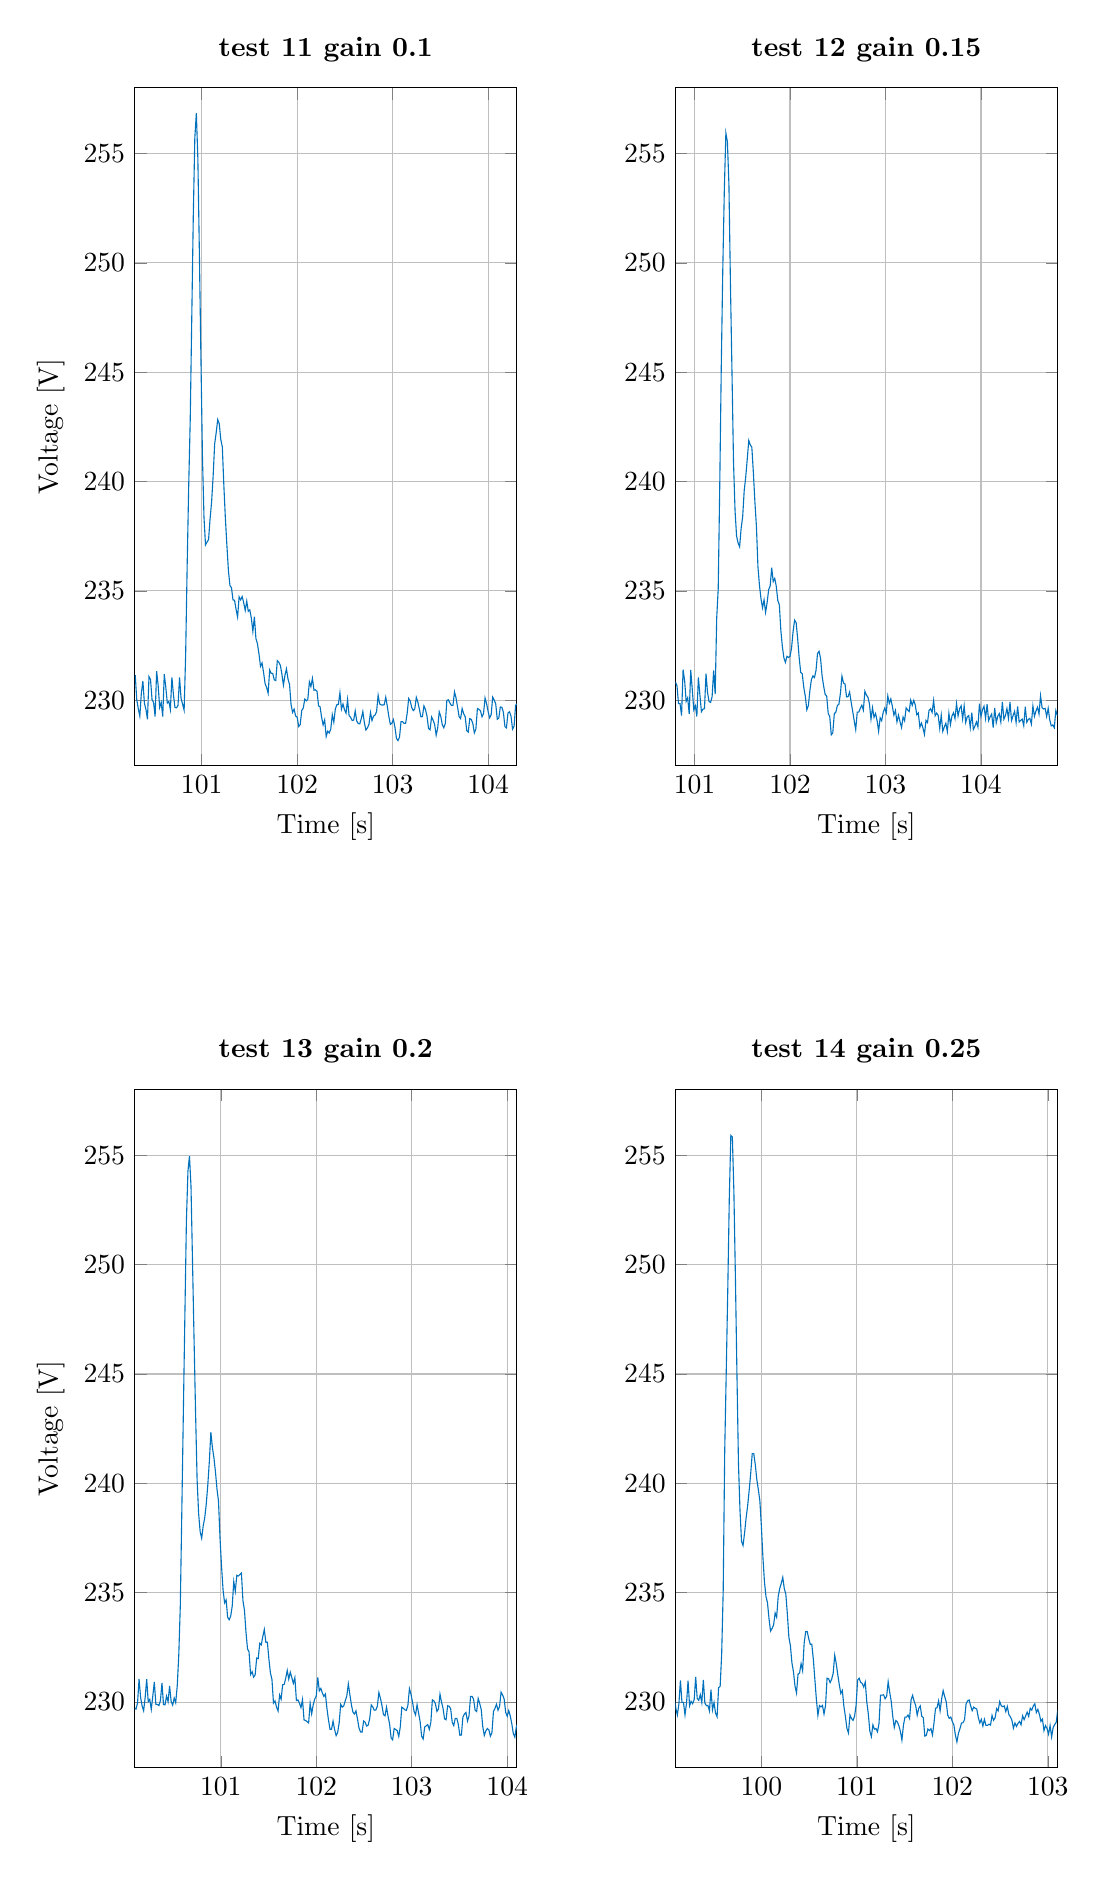
\begin{tikzpicture}

\begin{axis}[%
width=0.4\textwidth,
height=3.39in,
at={(1.297in,5.802in)},
scale only axis,
xmin=100.3,
xmax=104.3,
xlabel={Time [s]},
xmajorgrids,
ymin=227,
ymax=258,
ylabel={Voltage [V]},
ymajorgrids,
axis background/.style={fill=white},
title style={font=\bfseries},
title={test 11 gain 0.1}
]
\addplot [color=mycolor1,solid,forget plot]
  table[row sep=crcr]{%
100.288	230.353704051263\\
100.304	231.145373862542\\
100.32	230.024633075538\\
100.336	229.60501662414\\
100.352	229.275139969859\\
100.368	230.327368657412\\
100.384	230.877596393257\\
100.4	229.865809830275\\
100.416	229.586563231071\\
100.432	229.128987136977\\
100.448	231.07695645254\\
100.464	230.950589987495\\
100.48	230.027489765722\\
100.496	229.904026574225\\
100.512	229.255955863221\\
100.528	231.331745775034\\
100.544	230.682406014724\\
100.56	229.669996309881\\
100.576	229.905664706227\\
100.592	229.251611522028\\
100.608	231.191072301854\\
100.624	230.596113085706\\
100.64	229.872117246931\\
100.656	229.953070324751\\
100.672	229.57622646118\\
100.688	231.049419376761\\
100.704	230.258775554458\\
100.72	229.673774171051\\
100.736	229.653710785467\\
100.752	229.755526849545\\
100.768	231.041873080508\\
100.784	230.083614320636\\
100.8	229.822062426204\\
100.816	229.545296726939\\
100.832	232.080689148969\\
100.848	236.190068166592\\
100.864	239.805456345599\\
100.88	242.823172657949\\
100.896	247.45866342898\\
100.912	252.134142055695\\
100.928	255.709769050853\\
100.944	256.84263701152\\
100.96	254.750144065937\\
100.976	250.396251277893\\
100.992	245.659680650266\\
101.008	241.111006749821\\
101.024	238.370054166947\\
101.04	237.100801513144\\
101.056	237.235990701882\\
101.072	237.345009720522\\
101.088	238.30043143624\\
101.104	239.077112124773\\
101.12	240.254426980254\\
101.136	241.724086639012\\
101.152	242.23774373564\\
101.168	242.832721126851\\
101.184	242.642756974496\\
101.2	241.924577067276\\
101.216	241.585690261043\\
101.232	239.836907677749\\
101.248	238.324396317775\\
101.264	237.089631582878\\
101.28	235.924146549808\\
101.296	235.247510677118\\
101.312	235.142288211897\\
101.328	234.589304608607\\
101.344	234.574046996052\\
101.36	234.155897093457\\
101.376	233.805982455579\\
101.392	234.727489009027\\
101.408	234.589022412847\\
101.424	234.740012091747\\
101.44	234.46112159913\\
101.456	234.108295624246\\
101.472	234.533528862211\\
101.488	234.06642173394\\
101.504	234.132183444129\\
101.52	233.762399739154\\
101.536	233.14462903006\\
101.552	233.821252269923\\
101.568	232.824418066257\\
101.584	232.584204969802\\
101.6	232.120356858585\\
101.616	231.549293138154\\
101.632	231.70706612376\\
101.648	231.276679745632\\
101.664	230.763161334083\\
101.68	230.582719888893\\
101.696	230.322248782411\\
101.712	231.38461946056\\
101.728	231.233493414426\\
101.744	231.228086649314\\
101.76	230.937131189781\\
101.776	230.900975294982\\
101.792	231.812205858226\\
101.808	231.739989165118\\
101.824	231.600198057805\\
101.84	231.196384937025\\
101.856	230.690561785923\\
101.872	231.14323288109\\
101.888	231.435897369784\\
101.904	230.971009779542\\
101.92	230.720385009232\\
101.936	229.81052402102\\
101.952	229.442685009495\\
101.968	229.593496139602\\
101.984	229.280709656284\\
102	229.223905892905\\
102.016	228.802206863781\\
102.032	228.887235389943\\
102.048	229.531591833673\\
102.064	229.645128385705\\
102.08	230.054190312468\\
102.096	229.972704592468\\
102.112	230.047265067965\\
102.128	230.845713952987\\
102.144	230.627944205478\\
102.16	231.002815495944\\
102.176	230.459777955459\\
102.192	230.477627662055\\
102.208	230.410702662557\\
102.224	229.745828631024\\
102.24	229.701291859229\\
102.256	229.220777059653\\
102.272	228.868996982323\\
102.288	229.104484966229\\
102.304	228.341911852099\\
102.32	228.587417476774\\
102.336	228.5040104421\\
102.352	228.680121691028\\
102.368	229.344077660324\\
102.384	228.997830350411\\
102.4	229.608894131432\\
102.416	229.796099606215\\
102.432	229.815248144309\\
102.448	230.34604107208\\
102.464	229.591407141122\\
102.48	229.828843570285\\
102.496	229.565339168419\\
102.512	229.407781978002\\
102.528	230.04000482799\\
102.544	229.294595265067\\
102.56	229.22029097116\\
102.576	229.07279565724\\
102.592	229.09323289643\\
102.608	229.509586159023\\
102.624	229.052173358601\\
102.64	228.93361192108\\
102.656	228.91943500405\\
102.672	229.170754399227\\
102.688	229.483217679446\\
102.704	228.970450538342\\
102.72	228.640648856726\\
102.736	228.73895148895\\
102.752	228.895326247427\\
102.768	229.443586597794\\
102.784	229.068385290546\\
102.8	229.274448680595\\
102.816	229.324898578781\\
102.832	229.478300465665\\
102.848	230.230766338985\\
102.864	229.832561821278\\
102.88	229.78637975564\\
102.896	229.779818525538\\
102.912	229.797136753436\\
102.928	230.140500680558\\
102.944	229.722244481311\\
102.96	229.264860943797\\
102.976	228.896831725082\\
102.992	228.948413832891\\
103.008	229.120646388896\\
103.024	228.773464798672\\
103.04	228.257841294798\\
103.056	228.155743580583\\
103.072	228.312028436489\\
103.088	229.023353886515\\
103.104	229.020220741394\\
103.12	228.942853242069\\
103.136	228.942949404638\\
103.152	229.392676087819\\
103.168	230.079900206016\\
103.184	229.971782166095\\
103.2	229.667156545157\\
103.216	229.52913251542\\
103.232	229.604793554839\\
103.248	230.132825114408\\
103.264	229.917656435359\\
103.28	229.595103920061\\
103.296	229.24115976654\\
103.312	229.253926674378\\
103.328	229.739905923816\\
103.344	229.572646032104\\
103.36	229.277366754395\\
103.376	228.707661097877\\
103.392	228.65161980173\\
103.408	229.234920773622\\
103.424	229.090866669609\\
103.44	228.895297475203\\
103.456	228.400591862787\\
103.472	228.732275697813\\
103.488	229.47504591996\\
103.504	229.266655170836\\
103.52	228.884054793063\\
103.536	228.742465652075\\
103.552	228.943569307384\\
103.568	229.996533167167\\
103.584	230.021645078518\\
103.6	229.878984096962\\
103.616	229.763527850862\\
103.632	229.765835183156\\
103.648	230.385289810868\\
103.664	230.110498718106\\
103.68	229.693540484495\\
103.696	229.25002548337\\
103.712	229.16189368685\\
103.728	229.62132261678\\
103.744	229.387814715101\\
103.76	229.246901451996\\
103.776	228.615828374135\\
103.792	228.544980535963\\
103.808	229.161234004504\\
103.824	229.123644676645\\
103.84	228.935041608054\\
103.856	228.506691649953\\
103.872	228.685727882085\\
103.888	229.621194004665\\
103.904	229.586325688233\\
103.92	229.517068423091\\
103.936	229.242618769705\\
103.952	229.395757442525\\
103.968	230.10464698371\\
103.984	229.846506154978\\
104	229.487658940162\\
104.016	229.194931580038\\
104.032	229.335173387724\\
104.048	230.142758617338\\
104.064	230.010889025922\\
104.08	229.826774722516\\
104.096	229.1325453557\\
104.112	229.186290206057\\
104.128	229.690345843689\\
104.144	229.682631188102\\
104.16	229.452350249805\\
104.176	228.80162747298\\
104.192	228.73548764378\\
104.208	229.414342123026\\
104.224	229.471969626392\\
104.24	229.277547267117\\
104.256	228.681358165749\\
104.272	228.809100106433\\
104.288	229.763651278257\\
104.304	229.840108306363\\
};
\end{axis}

\begin{axis}[%
width=0.4\textwidth,
height=3.39in,
at={(4in,5.802in)},
scale only axis,
xmin=100.8,
xmax=104.8,
xlabel={Time [s]},
xmajorgrids,
ymin=227,
ymax=258,
ymajorgrids,
axis background/.style={fill=white},
title style={font=\bfseries},
title={test 12  gain 0.15}
]
\addplot [color=mycolor1,solid,forget plot]
  table[row sep=crcr]{%
100.8	230.829056078681\\
100.816	230.662105461448\\
100.832	229.847501423266\\
100.848	229.84533552108\\
100.864	229.302451765944\\
100.88	231.403272993676\\
100.896	230.907795097734\\
100.912	229.951931780346\\
100.928	230.116734861353\\
100.944	229.374038363318\\
100.96	231.387942663968\\
100.976	230.50566369866\\
100.992	229.561158612731\\
101.008	229.746958443018\\
101.024	229.25985169385\\
101.04	231.044120560205\\
101.056	230.245987267645\\
101.072	229.476112430819\\
101.088	229.594243116209\\
101.104	229.61789093333\\
101.12	231.21985131027\\
101.136	230.352755287142\\
101.152	229.939143076097\\
101.168	229.905702345035\\
101.184	230.167693082918\\
101.2	231.364564748675\\
101.216	230.282290766993\\
101.232	233.755663664812\\
101.248	235.11817124335\\
101.264	239.840090657609\\
101.28	245.290019494836\\
101.296	249.774391871552\\
101.312	253.355101789486\\
101.328	255.933495679891\\
101.344	255.536451815399\\
101.36	253.592276965441\\
101.376	249.016644654069\\
101.392	245.019446576999\\
101.408	240.908049559911\\
101.424	238.684301366811\\
101.44	237.510973657009\\
101.456	237.194398244958\\
101.472	237.019235772342\\
101.488	237.863709121441\\
101.504	238.388951725633\\
101.52	239.582229041833\\
101.536	240.207004891384\\
101.552	241.029243178656\\
101.568	241.880064968773\\
101.584	241.673903017572\\
101.6	241.568658568485\\
101.616	240.409961289743\\
101.632	239.076975449466\\
101.648	237.95909062651\\
101.664	236.101416780399\\
101.68	235.248865684507\\
101.696	234.636376775437\\
101.712	234.229665558565\\
101.728	234.588807696294\\
101.744	234.021203570678\\
101.76	234.461486031164\\
101.776	235.053140796147\\
101.792	235.230017502222\\
101.808	236.062600012774\\
101.824	235.427493506258\\
101.84	235.571808979734\\
101.856	235.208665564539\\
101.872	234.559790899157\\
101.888	234.366736858128\\
101.904	233.188598917349\\
101.92	232.448094232883\\
101.936	231.935347205131\\
101.952	231.729818236142\\
101.968	232.008869269878\\
101.984	231.955277937664\\
102	232.007263679472\\
102.016	232.389837779371\\
102.032	233.135241129964\\
102.048	233.66146154801\\
102.064	233.553256562489\\
102.08	232.820344787893\\
102.096	231.93638017471\\
102.112	231.272483262577\\
102.128	231.210335813684\\
102.144	230.588111512501\\
102.16	230.187552181623\\
102.176	229.56393233827\\
102.192	229.750988531863\\
102.208	230.440973201745\\
102.224	230.945511612983\\
102.24	231.11602711007\\
102.256	231.037714538771\\
102.272	231.361289560883\\
102.288	232.136816779748\\
102.304	232.238902022956\\
102.32	231.911377064212\\
102.336	231.107358572121\\
102.352	230.649817351196\\
102.368	230.26849805499\\
102.384	230.192795526096\\
102.4	229.399901261292\\
102.416	229.252590956798\\
102.432	228.418417171983\\
102.448	228.514283805639\\
102.464	229.387693660309\\
102.48	229.454718205086\\
102.496	229.76119626912\\
102.512	229.818557609383\\
102.528	230.324000895863\\
102.544	231.107072720961\\
102.56	230.793070300903\\
102.576	230.743587289282\\
102.592	230.153601519018\\
102.608	230.16469065255\\
102.624	230.37841290281\\
102.64	229.923530001487\\
102.656	229.502603307927\\
102.672	229.068504172519\\
102.688	228.657355054025\\
102.704	229.457040860129\\
102.72	229.457866491789\\
102.736	229.629330915208\\
102.752	229.771308435219\\
102.768	229.546452810036\\
102.784	230.412425653022\\
102.8	230.237498945756\\
102.816	230.139366676825\\
102.832	229.831031621351\\
102.848	229.133702206933\\
102.864	229.657369884951\\
102.88	229.218604685106\\
102.896	229.396376275001\\
102.912	229.064149709656\\
102.928	228.580127471418\\
102.944	229.198011872452\\
102.96	229.062863305411\\
102.976	229.450729979804\\
102.992	229.639498446383\\
103.008	229.426048088237\\
103.024	230.19640296265\\
103.04	229.859749220226\\
103.056	230.063756242989\\
103.072	229.718782194551\\
103.088	229.319986831586\\
103.104	229.53619805165\\
103.12	229.010851769471\\
103.136	229.323312860746\\
103.152	229.022653808416\\
103.168	228.752579419744\\
103.184	229.230688940544\\
103.2	229.059037282268\\
103.216	229.653416468949\\
103.232	229.556513821786\\
103.248	229.484920530367\\
103.264	230.005353484673\\
103.28	229.76673734569\\
103.296	229.992390349551\\
103.312	229.780651681711\\
103.328	229.334772652128\\
103.344	229.418009642116\\
103.36	228.76579832182\\
103.376	228.954841281479\\
103.392	228.740276716186\\
103.408	228.439998284027\\
103.424	229.077609008319\\
103.44	228.981475851038\\
103.456	229.541717452577\\
103.472	229.613014188692\\
103.488	229.445446151789\\
103.504	229.989969802642\\
103.52	229.289305655662\\
103.536	229.412911129361\\
103.552	229.307120649319\\
103.568	228.713439213142\\
103.584	229.318532438818\\
103.6	228.579998282175\\
103.616	228.77557385841\\
103.632	228.94849478949\\
103.648	228.564788540418\\
103.664	229.401442110779\\
103.68	228.884842773428\\
103.696	229.279969923627\\
103.712	229.429060288766\\
103.728	229.164431805897\\
103.744	229.845685561592\\
103.76	229.283754981999\\
103.776	229.612494558023\\
103.792	229.745188606528\\
103.808	229.14617662421\\
103.824	229.742019278591\\
103.84	228.983647303758\\
103.856	229.238303051713\\
103.872	229.30075978866\\
103.888	228.747810607162\\
103.904	229.431239634742\\
103.92	228.664138264231\\
103.936	228.805455683156\\
103.952	229.010879926733\\
103.968	228.778909440048\\
103.984	229.843648935178\\
104	229.262546491603\\
104.016	229.570499635352\\
104.032	229.727872617553\\
104.048	229.167958531953\\
104.064	229.820438622538\\
104.08	229.070068574288\\
104.096	229.240262822051\\
104.112	229.369289380199\\
104.128	228.750242247105\\
104.144	229.648989342186\\
104.16	228.970333665668\\
104.176	229.27122759535\\
104.192	229.392704375326\\
104.208	229.003485288981\\
104.224	229.923226307189\\
104.24	229.13307984725\\
104.256	229.297614477141\\
104.272	229.620298941351\\
104.288	229.168618413742\\
104.304	229.92011282439\\
104.32	229.073786512126\\
104.336	229.290683824593\\
104.352	229.495642129401\\
104.368	228.984851806458\\
104.384	229.71551161342\\
104.4	229.008034965536\\
104.416	229.078917552137\\
104.432	229.13680388318\\
104.448	228.839816116269\\
104.464	229.703869773759\\
104.48	228.994313103008\\
104.496	229.125068552887\\
104.512	229.173979743958\\
104.528	228.912487984476\\
104.544	229.737462782588\\
104.56	229.266028955856\\
104.576	229.508933712947\\
104.592	229.682360449665\\
104.608	229.373326795033\\
104.624	230.212027962756\\
104.64	229.659369869918\\
104.656	229.597855790809\\
104.672	229.627576985913\\
104.688	229.260204392904\\
104.704	229.633266724632\\
104.72	229.111960800537\\
104.736	228.827812629325\\
104.752	228.870266409584\\
104.768	228.743968795529\\
104.784	229.528671422795\\
104.8	229.313980275243\\
104.816	229.257250710075\\
};
\end{axis}

\begin{axis}[%
width=0.4\textwidth,
height=3.39in,
at={(1.297in,0.793in)},
scale only axis,
xmin=100.1,
xmax=104.1,
xlabel={Time [s]},
xmajorgrids,
ymin=227,
ymax=258,
ylabel={Voltage [V]},
ymajorgrids,
axis background/.style={fill=white},
title style={font=\bfseries},
title={test 13  gain 0.2}
]
\addplot [color=mycolor1,solid,forget plot]
  table[row sep=crcr]{%
100.096	229.728780390738\\
100.112	229.681690390074\\
100.128	229.949580814653\\
100.144	231.05560626423\\
100.16	230.213536789278\\
100.176	229.82286782401\\
100.192	229.599332693859\\
100.208	230.217151083259\\
100.224	231.050952198395\\
100.24	230.011577683913\\
100.256	230.122080920462\\
100.272	229.667791577033\\
100.288	230.281150882047\\
100.304	230.91821527395\\
100.32	229.897179088397\\
100.336	229.889414210284\\
100.352	229.838407930822\\
100.368	230.073106140613\\
100.384	230.872163897837\\
100.4	229.885383004923\\
100.416	229.872795438076\\
100.432	230.273754428435\\
100.448	230.01617382841\\
100.464	230.743214174753\\
100.48	230.028053470396\\
100.496	229.862001702851\\
100.512	230.182697328057\\
100.528	229.972126530698\\
100.544	230.741590115368\\
100.56	232.153763371814\\
100.576	234.402035404171\\
100.592	238.756672240036\\
100.608	243.257325955509\\
100.624	247.694693196384\\
100.64	252.018767047599\\
100.656	254.265011204601\\
100.672	254.963182573613\\
100.688	253.588934627946\\
100.704	250.125377675081\\
100.72	246.59389655317\\
100.736	243.218744628851\\
100.752	240.153238898738\\
100.768	238.612660641234\\
100.784	237.785221308462\\
100.8	237.491186347023\\
100.816	238.062111916408\\
100.832	238.427088854713\\
100.848	239.064382526245\\
100.864	239.926546842883\\
100.88	240.991931774492\\
100.896	242.335831213284\\
100.912	241.64920568211\\
100.928	241.174214133003\\
100.944	240.538044469698\\
100.96	239.751580033485\\
100.976	239.187027540751\\
100.992	237.494804687872\\
101.008	236.199341160766\\
101.024	235.115329790974\\
101.04	234.536974013917\\
101.056	234.669843754292\\
101.072	233.875352451714\\
101.088	233.764751882757\\
101.104	233.932828167326\\
101.12	234.396792885007\\
101.136	235.51144169621\\
101.152	235.06610010926\\
101.168	235.796882939154\\
101.184	235.760924928972\\
101.2	235.830088946538\\
101.216	235.899703725534\\
101.232	234.642922669526\\
101.248	234.197760989362\\
101.264	233.192988417647\\
101.28	232.430002399107\\
101.296	232.289516977322\\
101.312	231.257084733279\\
101.328	231.389339659649\\
101.344	231.138374938862\\
101.36	231.241298374106\\
101.376	232.013379302245\\
101.392	231.987158997011\\
101.408	232.686159652314\\
101.424	232.615442530452\\
101.44	232.994135600596\\
101.456	233.319842182856\\
101.472	232.733553601479\\
101.488	232.737655656342\\
101.504	231.968318017967\\
101.52	231.32561952491\\
101.536	231.035871369644\\
101.552	229.953784970251\\
101.568	230.054746968393\\
101.584	229.767881833938\\
101.6	229.589205437488\\
101.616	230.321505586003\\
101.632	230.128434968111\\
101.648	230.790714523366\\
101.664	230.806635087924\\
101.68	231.084113501287\\
101.696	231.449450185295\\
101.712	231.047036284103\\
101.728	231.364765838225\\
101.744	231.116406661971\\
101.76	230.853856481246\\
101.776	231.115656541001\\
101.792	230.071228516006\\
101.808	230.098334678552\\
101.824	229.94734925578\\
101.84	229.74436092732\\
101.856	230.118411443993\\
101.872	229.182595651197\\
101.888	229.158758409861\\
101.904	229.10317276131\\
101.92	229.046804489583\\
101.936	229.945144124422\\
101.952	229.461954399364\\
101.968	229.874111137037\\
101.984	230.138426412601\\
102	230.273728035193\\
102.016	231.125513855452\\
102.032	230.510434422707\\
102.048	230.623669545353\\
102.064	230.416430393821\\
102.08	230.257485367601\\
102.096	230.368124735663\\
102.112	229.70259611934\\
102.128	229.185145919578\\
102.144	228.753036608514\\
102.16	228.758617548546\\
102.176	229.12787916139\\
102.192	228.747521730085\\
102.208	228.466094696056\\
102.224	228.607974893389\\
102.24	229.052410688768\\
102.256	229.893325169046\\
102.272	229.769325575801\\
102.288	229.828063413211\\
102.304	230.057736547382\\
102.32	230.283591474238\\
102.336	230.830055241798\\
102.352	230.343696008435\\
102.368	229.879114776689\\
102.384	229.539689774842\\
102.4	229.451310668178\\
102.416	229.599809760749\\
102.432	229.220677041432\\
102.448	228.812049442809\\
102.464	228.633068164977\\
102.48	228.624129269948\\
102.496	229.136182450342\\
102.512	229.076558844521\\
102.528	228.903122594268\\
102.544	228.948390536603\\
102.56	229.245517263741\\
102.576	229.871487468545\\
102.592	229.774034178173\\
102.608	229.627414858177\\
102.624	229.636915759233\\
102.64	229.81264429895\\
102.656	230.436099015281\\
102.672	230.178186672243\\
102.688	229.847683431116\\
102.704	229.428755390755\\
102.72	229.370551896794\\
102.736	229.762908019685\\
102.752	229.353549690531\\
102.768	229.000049894194\\
102.784	228.360686789393\\
102.8	228.272519571526\\
102.816	228.790637277088\\
102.832	228.744048150675\\
102.848	228.695510910445\\
102.864	228.427328898924\\
102.88	228.861898728402\\
102.896	229.763978105196\\
102.912	229.712998488679\\
102.928	229.649600674693\\
102.944	229.617640957189\\
102.96	229.853770413942\\
102.976	230.613022673544\\
102.992	230.364515989439\\
103.008	230.001874867822\\
103.024	229.58444195469\\
103.04	229.41085956095\\
103.056	229.881151990341\\
103.072	229.495094923177\\
103.088	229.107067871987\\
103.104	228.438221892064\\
103.12	228.31127537222\\
103.136	228.859446081707\\
103.152	228.912910269133\\
103.168	228.970714598992\\
103.184	228.749378124025\\
103.2	229.062391422658\\
103.216	230.100756369793\\
103.232	230.057977165425\\
103.248	229.92280936592\\
103.264	229.57143386244\\
103.28	229.68053621946\\
103.296	230.359420812688\\
103.312	229.999543426344\\
103.328	229.715531613085\\
103.344	229.228829161537\\
103.36	229.193617268324\\
103.376	229.832928095715\\
103.392	229.808774278008\\
103.408	229.692921578194\\
103.424	229.071986753443\\
103.44	228.925576971227\\
103.456	229.252505042966\\
103.472	229.255198215188\\
103.488	228.976623402775\\
103.504	228.483925282448\\
103.52	228.487401639992\\
103.536	229.318555478221\\
103.552	229.451336484878\\
103.568	229.521429619891\\
103.584	229.127753637732\\
103.6	229.369242016099\\
103.616	230.26121256205\\
103.632	230.260379267047\\
103.648	230.120076650953\\
103.664	229.627073979167\\
103.68	229.566779667381\\
103.696	230.163166758228\\
103.712	229.938445684264\\
103.728	229.65622989756\\
103.744	228.876086327104\\
103.76	228.474935475115\\
103.776	228.680959118003\\
103.792	228.792703143475\\
103.808	228.728310017459\\
103.824	228.440171995332\\
103.84	228.597016963118\\
103.856	229.564493563031\\
103.872	229.714898109455\\
103.888	229.903702299102\\
103.904	229.62651127061\\
103.92	229.79636906816\\
103.936	230.453527340134\\
103.952	230.324776910144\\
103.968	230.14493849384\\
103.984	229.526810036872\\
104	229.351607949106\\
104.016	229.611665041083\\
104.032	229.36199383974\\
104.048	229.013236086339\\
104.064	228.561069749084\\
104.08	228.395645920516\\
104.096	228.867588644414\\
104.112	229.045033268479\\
};
\end{axis}

\begin{axis}[%
width=0.4\textwidth,
height=3.39in,
at={(4in,0.793in)},
scale only axis,
xmin=99.1,
xmax=103.1,
xlabel={Time [s]},
xmajorgrids,
ymin=227,
ymax=258,
ymajorgrids,
axis background/.style={fill=white},
title style={font=\bfseries},
title={test 14  gain 0.25}
]
\addplot [color=mycolor1,solid,forget plot]
  table[row sep=crcr]{%
99.088	230.26103802426\\
99.104	229.710410269688\\
99.12	229.408283277938\\
99.136	229.911077944173\\
99.152	230.994252987228\\
99.168	229.985782127239\\
99.184	229.980022256471\\
99.2	229.414375757875\\
99.216	229.955405150201\\
99.232	230.97598561848\\
99.248	229.825795017092\\
99.264	230.031225117501\\
99.28	229.926421244662\\
99.296	230.107894890942\\
99.312	231.145114112706\\
99.328	230.158710942542\\
99.344	230.081900581214\\
99.36	230.336907019547\\
99.376	229.973155164386\\
99.392	231.016319232828\\
99.408	229.953188273349\\
99.424	229.835268685766\\
99.44	229.848749509344\\
99.456	229.592543914211\\
99.472	230.566324071443\\
99.488	229.644543601465\\
99.504	229.976380178602\\
99.52	229.493152083517\\
99.536	229.326803411641\\
99.552	230.665097727968\\
99.568	230.711943302453\\
99.584	232.183150278641\\
99.6	235.074166609092\\
99.616	241.480810294827\\
99.632	245.108860112587\\
99.648	248.858343420219\\
99.664	253.05147031973\\
99.68	255.909963966424\\
99.696	255.837177261774\\
99.712	253.33588241122\\
99.728	249.412254833126\\
99.744	245.013605761982\\
99.76	240.903815343687\\
99.776	238.763162131846\\
99.792	237.351869930762\\
99.808	237.15932950352\\
99.824	237.730026088033\\
99.84	238.424199993361\\
99.856	238.968656706561\\
99.872	239.670772895381\\
99.888	240.447486575218\\
99.904	241.356010493501\\
99.92	241.359411305434\\
99.936	240.864869867877\\
99.952	240.178251887909\\
99.968	239.722946055951\\
99.984	239.205384241232\\
100	238.034535290144\\
100.016	236.619221246651\\
100.032	235.509884723747\\
100.048	234.824203093766\\
100.064	234.539505323651\\
100.08	233.808848428025\\
100.096	233.246224949625\\
100.112	233.366807074215\\
100.128	233.5201098099\\
100.144	234.073856542999\\
100.16	233.876535435058\\
100.176	234.82367686485\\
100.192	235.191744232875\\
100.208	235.421828924166\\
100.224	235.706378538352\\
100.24	235.184861824163\\
100.256	234.932345304591\\
100.272	234.025413436865\\
100.288	232.961480384987\\
100.304	232.582572342442\\
100.32	231.787624529075\\
100.336	231.388958120717\\
100.352	230.731341755838\\
100.368	230.41493001132\\
100.384	231.278371154708\\
100.4	231.330295068454\\
100.416	231.757502257106\\
100.432	231.432235522302\\
100.448	232.690681943014\\
100.464	233.219024618526\\
100.48	233.230095875444\\
100.496	232.897256354831\\
100.512	232.641656077615\\
100.528	232.642477570447\\
100.544	231.964905441938\\
100.56	231.049419787682\\
100.576	230.121354525952\\
100.592	229.393399205835\\
100.608	229.84278565531\\
100.624	229.77698920405\\
100.64	229.845671421106\\
100.656	229.451934885894\\
100.672	229.839162276245\\
100.688	231.092315326484\\
100.704	231.066712616234\\
100.72	230.890480411731\\
100.736	231.044666685497\\
100.752	231.31264607574\\
100.768	232.143501287948\\
100.784	231.761835831293\\
100.8	231.253316308307\\
100.816	230.791049817819\\
100.832	230.393492029082\\
100.848	230.52878024176\\
100.864	229.810831586841\\
100.88	229.341479139112\\
100.896	228.791539402364\\
100.912	228.5852121948\\
100.928	229.409747895512\\
100.944	229.244824412913\\
100.96	229.16148624542\\
100.976	229.350229888306\\
100.992	229.853157583832\\
101.008	231.002401762084\\
101.024	231.090692762401\\
101.04	230.900490562455\\
101.056	230.852903217704\\
101.072	230.682707501658\\
101.088	230.913348189715\\
101.104	230.010033535863\\
101.12	229.458076733087\\
101.136	228.673023035141\\
101.152	228.419028934478\\
101.168	228.956038074128\\
101.184	228.757920893961\\
101.2	228.79108203374\\
101.216	228.637951995906\\
101.232	229.017360063957\\
101.248	230.313204692699\\
101.264	230.315157944054\\
101.28	230.333745447489\\
101.296	230.152440110197\\
101.312	230.262465785668\\
101.328	230.929722820605\\
101.344	230.447219388864\\
101.36	230.032308043889\\
101.376	229.35299096803\\
101.392	228.836352684498\\
101.408	229.152568767118\\
101.424	229.090468695785\\
101.44	228.91806962025\\
101.456	228.66159860077\\
101.472	228.257622116507\\
101.488	228.944899546023\\
101.504	229.312988069813\\
101.52	229.312113061078\\
101.536	229.407196407343\\
101.552	229.24574339823\\
101.568	230.096832981046\\
101.584	230.306441922734\\
101.6	230.037699347689\\
101.616	229.847086879608\\
101.632	229.39772432748\\
101.648	229.709018955833\\
101.664	229.824016171503\\
101.68	229.350876764005\\
101.696	229.283911040705\\
101.712	228.440598345623\\
101.728	228.478785901445\\
101.744	228.76921741415\\
101.76	228.698506610101\\
101.776	228.781837962099\\
101.792	228.493892869026\\
101.808	229.050000543713\\
101.824	229.716391350112\\
101.84	229.744912841743\\
101.856	230.055762623369\\
101.872	229.594907623002\\
101.888	230.143629947557\\
101.904	230.52355068446\\
101.92	230.25790753953\\
101.936	230.010634495302\\
101.952	229.400638084515\\
101.968	229.254510179817\\
101.984	229.312346106048\\
102	229.105226702434\\
102.016	228.961054220616\\
102.032	228.494061703796\\
102.048	228.177126139704\\
102.064	228.566873353116\\
102.08	228.784841060341\\
102.096	229.039868898183\\
102.112	229.056070245768\\
102.128	229.195130749521\\
102.144	229.913771113003\\
102.16	230.051743439483\\
102.176	230.093849556964\\
102.192	229.82630147178\\
102.208	229.607720842182\\
102.224	229.769300162289\\
102.24	229.712322832596\\
102.256	229.679543666257\\
102.272	229.294405941554\\
102.288	229.042586464815\\
102.304	229.211005952545\\
102.32	228.903199803289\\
102.336	229.208006893838\\
102.352	228.932125996995\\
102.368	228.934376364748\\
102.384	228.986187053283\\
102.4	228.949851505061\\
102.416	229.390815004736\\
102.432	229.167466310223\\
102.448	229.281346944791\\
102.464	229.700411919858\\
102.48	229.596852230015\\
102.496	230.024453645096\\
102.512	229.831245588443\\
102.528	229.787337931249\\
102.544	229.822155290511\\
102.56	229.561428276061\\
102.576	229.797347115695\\
102.592	229.427764216225\\
102.608	229.32689392553\\
102.624	229.16864577959\\
102.64	228.807715955555\\
102.656	229.042611672899\\
102.672	228.885888702368\\
102.688	229.021921420284\\
102.704	229.113703217771\\
102.72	228.961211221651\\
102.736	229.369460971061\\
102.752	229.195650166866\\
102.768	229.365596232158\\
102.784	229.538682202443\\
102.8	229.34352861245\\
102.816	229.718463697671\\
102.832	229.633179028161\\
102.848	229.820088415292\\
102.864	229.921733084944\\
102.88	229.51942793261\\
102.896	229.664847000749\\
102.912	229.440779556942\\
102.928	229.116268091551\\
102.944	229.217895358156\\
102.96	228.691532959621\\
102.976	228.922331134096\\
102.992	228.793494157768\\
103.008	228.532858290125\\
103.024	228.927003752838\\
103.04	228.40387120055\\
103.056	228.832449460738\\
103.072	228.972194760061\\
103.088	229.070023981726\\
103.104	229.622590838969\\
};
\end{axis}
\end{tikzpicture}%
\caption{Step from 50 to 10 kW load, with various scaling factors.}
\label{fig:test11-14-50to10kwstepvolt}
\end{figure}


\subsection*{Results:}

When the scaling factor ranges from 0.1 to 0.25 the genset are stable, but when the scaling factor is increased to 0.3 after 12 seconds, the genset start to fluctuate in frequency. When the gain is increased further to 0.35 at 20 seconds the genset starts to fluctuate more rapid as shown on \figref{fig:test15-instablecontroller}. Furthermore the genset started shaking due to the controller reacting to intense on the input therefore gains higher or equal to 0.3 are disregarded. The scaling factor giving the most steady output on frequency, Voltage and power is 0.1, which is shown on the lower overshoot in frequency which is clearly shown on \figref{fig:test11-14-10to20kwstepfreq}. Visible influence due to the nature of the second order model is more apperent at higher values of the scaling factor as shown on \figref{fig:test11-14-20to30kwstepvolt}. At 10 kW load the lower scaling factor shows improved steady state stability over higher values, which is shown on \figref{fig:test11-14steadyfrequency10kw} and \figref{fig:test11-14steadyvolt10kw}.

\subsection*{Conclusion}
It shows clearly that the designed controller has a larger impact in lowering disturbance at lower scaling factors but only at certain load levels. The higher scaling factors shows the dynamics of the second order model derived for the use of designing the controller, giving a more fluctuating output on the genset. The scaling factor of 0.1 should be chosen af the prefered value for the designed controller.    